\NeedsTeXFormat{LaTeX2e}[1996/06/01]
\documentclass[cup6a]{cupbook}

\usepackage{alltt}
\usepackage{amsfonts}
\usepackage{amsmath}
\usepackage{amssymb}
\usepackage{boxedminipage}
\usepackage{eurosym}
\usepackage{float}
\usepackage{geometry}
\geometry{left=1in,right=1.75in,top=1.25in,bottom=1.25in}
\usepackage{graphicx}
\usepackage{lscape}
\usepackage{makeidx}
\usepackage{multicol}
\usepackage{natbib}
\usepackage{rotating}
\usepackage{scalefnt}
\usepackage{setspace}
\usepackage{hhline}
\usepackage{color}
\usepackage{url}
\usepackage{paralist}
\usepackage{epic}

%  NEEDED ONLY FOR CHAPTER 21
%  HIT RETURN TWICE
\usepackage{subfig}
\captionsetup[subfloat]{justification=raggedright}
\usepackage{caption}
\usepackage[margin=10pt,font=small,labelfont=bf]{caption}

\newcommand{\marginparjed}[1]
{\marginpar{\renewcommand{\baselinestretch}{0.6}\normalsize\raggedright\textit{\footnotesize
#1}}}

\newcommand{\linejed}
{\noindent
\rule{5.5in}{.008in}\vspace{-.15in}\newline\rule{5.5in}{.008in}}

\newcommand{\linetjed}
{\noindent
\rule{5.5in}{.008in}\vspace{-.1in}\newline\rule{5.5in}{.008in}}

\newcommand{\boxedjed}
{\begin{boxedminipage}{5.25in}}

\newcommand\ecaptionjed[1]
  {\addcontentsline{xmp}{example}{#1}}
  \makeatletter \newcommand\listofexamples
  {\section*{Examples}\@starttoc{xmp}}
  \newcommand\l@example[2]
  {\par\noindent#1,~\textit{#2}\par} \makeatother

\newcommand{\empexjed}[1]
{ \marginparjed{\newline \newline \circledR
\scalefont{0.90}{\textsc{ \textbf{Empirical}} \newline Filename is
\newline ``#1''}\scalefont{1.1111}}}

\title{Regression Modeling with Actuarial and Financial Applications}

\author{Edward W. Frees}
\date{\today}
\makeindex

\begin{document}
\setlength{\marginparwidth}{1in}
\setlength{\marginparsep}{0.25in}


\pagenumbering{roman} \maketitle

\pagenumbering{arabic}

\tableofcontents

\chapter*{Dedication}


There is an old saying, attributed to Sir Issac Newton and that can
be found on web at Google Scholar,


\bigskip\bigskip

\begin{center}
``If I have seen far, it is by standing on the shoulders of
giants.''
\end{center}

\bigskip\bigskip

\noindent I dedicate this book to the memory of two giants who
helped me, and everyone who knew them, see farther and live better
lives:
\bigskip\bigskip


\begin{center}James C. Hickman\end{center}


and



\begin{center}Joseph P. Sullivan.\end{center}



\chapter*{Preface}

\vspace{-1in}

Actuaries and other financial analysts quantify situations using
data -- we are ``numbers'' people. Many of our approaches and models
are stylized, based on years of experience and investigations
performed by legions of analysts. However, the financial and risk
management world evolves rapidly. Many analysts are confronted with
new situations in which tried-and-true methods simply do not work.
This is where a toolkit like regression analysis comes in.

Regression is the study of relationships among variables. It is a
generic statistics discipline that is not restricted to the
financial world -- it has applications in fields of social,
biological and physical sciences. You can use regression techniques
to investigate large and complex data sets. To familiarize you with
regression, this book explores many examples and data sets based on
actuarial and financial applications. This is not to say that you
will not encounter applications outside of the financial world (for
example, an actuary may need to understand the latest scientific
evidence on genetic testing for underwriting purposes). However, as
you become acquainted with this toolkit, you will see how regression
can be applied in many (and sometimes new) situations.

\section*{Who Is This Book For?}

This book is written for financial analysts who face uncertain
events and wish to quantify these events using empirical
information. No industry knowledge is assumed although readers will
find the reading much easier if they have an interest in the
applications discussed here! This book is designed for students who
are just being introduced to the field as well as industry analysts
who would like to brush up on old techniques and (for the later
chapters) get an introduction to new developments.

To read this book, I assume knowledge comparable to a one semester
introduction to probability and statistics - Appendix A1 provides a
brief review to brush up if you are rusty. Actuarial students in
North America will have a one-year introduction to probability and
statistics - this type of introduction will help readers grasp
concepts more quickly than a one semester background. Finally,
readers will find matrix, or linear, algebra helpful, although not a
prerequisite for reading this text.

Different readers are interested in understanding statistics at
different levels. This book is written to accommodate the ``armchair
reader,'' that is, one who passively reads and does not get involved
by attempting the exercises in the text. Consider an analogy to
football, or any other game. Just like the armchair quarterback of
football, there is a great deal that you can learn about the game
just by watching. However, if you want to sharpen your skills, you
have to go out and play the game. If you do the exercises or
reproduce the statistical analyses in the text, you will become a
better player. Still, this text is written by interweaving examples
with the basic principles. Thus, even the armchair reader can obtain
a solid understanding of regression techniques through this text.

\section*{What Is This Book About?}

The Table of Contents provides an overview of the topics covered,
organized into four parts. The first part introduces linear
regression. This is the core material of the book, with refreshers
on mathematical statistics, distributions and matrix algebra woven
in as needed.

The second part is devoted to topics in times series. Why integrate
time series topics into a regression book? The reasons are simple,
yet compelling; most accounting, financial and economic data become
available over time. Although cross-sectional inferences are useful,
business decisions need to be made in real time with currently
available data. Chapters 7-10 introduce time series techniques that
can be readily accomplished using regression tools (and there are
many).

Nonlinear regression is the subject of the third part. Many modern
day ``predictive modeling'' tools are based on nonlinear regression
- these are the workhorses of statistical shops in the financial and
risk management industry.

The fourth part concerns ``actuarial applications,'' topics that I
have found relevant in my research and consulting work in financial
risk management. The first four chapters of this part consists of
variations of regression models that are particularly useful in risk
management. The last two chapters focus on communications,
specifically, report writing and designing graphs. Communicating
information is an important aspect of every technical discipline and
statistics is certainly no exception.


\section*{How Does This Book Deliver Its Message?}


\textbf{Chapter Development}. Each chapter has several examples
interwoven with theory. In chapters where a model is introduced, I
begin with an example and discuss the data analysis without regard
to the theory. This analysis is presented at an intuitive level,
without reference to a specific model. This is straightforward,
because it amounts to little more than curve fitting. The theme is
to have students summarize data sensibly without having the notion
of a model obscure good data analysis. Then, an introduction to the
theory is provided in the context of the introductory example. One
or more additional examples follow that reinforce the theory already
introduced and provide a context for explaining additional theory.
In Chapters 5 and 6, that do not introduce models but rather
techniques for analysis, I begin with an introduction of the
technique. This introduction is then followed by an example that
reinforces the explanation. In this way, the data analysis can be
easily omitted without loss of continuity, if time is a concern.

\textbf{Real Data}. Many of the exercises ask the reader to work
with real data. The need for working with real data is well
documented; for example, see Hogg (1972) or Singer and Willett
(1990). Some criteria of Singer and Willett for judging a good data
set include: (1) authenticity, (2) availability of background
information, (3) interest and relevance to substantive learning, and
(4) availability of elements with which readers can identify. Of
course, there are some important disadvantages to working with real
data. Data sets can quickly become outdated. Further, the ideal data
set to illustrate a specific statistical issue is difficult to find.
This is because with real data, almost by definition, several issues
occur simultaneously. This makes it difficult to isolate a specific
aspect. I particularly enjoy working with large data sets. The
larger the data set, the greater is the need for statistics to
summarize the information content.

\marginparjed{The larger the data set, the greater is the need for
statistics to summarize the information content.}


\textbf{Statistical Software and Data}. My goal in writing this text
is to reach a broad group of students and industry analysts. Thus,
to avoid excluding large segments, I chose not to integrate any
specific statistical software package into the text. Nonetheless,
because of the applications orientation, it is critical that the
methodology presented be easily accomplished using readily available
packages. For the course taught at the University of Wisconsin, I
use the statistical packages SAS and ``R.'' On the book web site,

\bigskip

{ \url{http://research.bus.wisc.edu/RegActuaries}}

\bigskip

\empexjed{TermLife}

\noindent users will find scripts written in SAS and R for the
analysis presented in the text. The data are available in text
format, allowing readers to employ any statistical packages that
they wish. When you see a display such as this in the margin, you
will also be able to find this data set (\emph{TermLife}) on the
book web site.

\textbf{Technical Supplements}. The technical supplements reinforce
and extend the results in the main body of the text by giving a more
formal, mathematical treatment of the material. This treatment is in
fact a supplement because the applications and examples are
described in the main body of the text. For readers with sufficient
mathematical background, the supplements provide additional material
that is useful in communicating to technical audiences. The
technical supplements provide a deeper, and broader, coverage of
applied regression analysis.

I believe that analysts should have an idea of ``what is going on
under the hood,'' or ``how the engine works.'' Most of these topics
will be omitted from the first reading of the material. However, as
you work with regression, you will be confronted with questions on
``Why?'' and you will need to get into the details to see exactly
how a certain technique works. Further, the technical supplements
provide a menu of optional items that an instructor may wish to
cover.


\textbf{Suggested Courses}. There is a wide variety of topics that
can go into a regression course. Here are some suggested courses.
The course that I teach at the University of Wisconsin is the first
on the list in the following table.

\begin{table}[h]
\scalefont{0.9}

\begin{tabular}{lll}
\hline
\multicolumn{1}{c}{Audience} & \multicolumn{1}{c}{Nature of Course}& \multicolumn{1}{c}{Suggested Chapters} \\
\hline One-year background in & Survey of regression and  &
 Chapters
1-8 ,11-13, 20-21,\\
~~~probability and statistics & ~~~time series models &
~~~main body of text only \\
One-year background in & Regression and time  &
 Chapters
1-8, 20-21, selected \\
~~~probability and statistics & ~~~series models &
~~~portions of technical supplements \\
One-year background in & Regression modeling  &
 Chapters
1-6, 11-13, 20-21, selected \\
~~~probability and statistics & &
~~~ portions of technical supplements \\
Background in statistics& Actuarial regression&
 Chapters
10-21, selected \\
~~~and linear regression&  ~~~models  &
~~~ portions of technical supplements \\
 \hline
\end{tabular}
\scalefont{1.1111}
\end{table}

In addition to these suggested courses, this book is designed for
supplemental reading for a time series course as well as a reference
book for industry analysts. My hope is that college students who use
the beginning parts of the book in their university course will find
the later chapters helpful in their industry positions. In this way
I hope to promote life-long learning!



\section*{Acknowledgements}

It is appropriate to begin the acknowledgement section by thanking
the students in the actuarial program here at the University of
Wisconsin; students are important partners in the knowledge creation
and dissemination business at universities. Through their questions
and feedback, I have learned a tremendous amount over the years. I
have also benefited from \emph{excellent} assistance from those who
have helped me pull together all the pieces for this book,
specifically, Missy Pinney, Peng Shi, Yunjie (Winnie) Sun and Ziyan
Xie.

I have enjoyed working with several former students and colleagues
on regression problems over the recent years, including Katrien
Antonio, Jie Gao, Paul Johnson, Margie Rosenberg, Jiafeng Sun, Emil
Valdez and Ping Wang. Their contributions are reflected indirectly
throughout the text. Because of my long association with the
University of Wisconsin-Madison, I am reluctant to go back further
in time and provide a longer list for fear of missing important
individuals. I have also been fortunate to have a more recent
association with the Insurance Services Office (ISO). Colleagues at
ISO have provided me with important insights into applications.
Through this text that features applications of regression into
actuarial and financial industry problems, I hope to encourage the
fostering of additional partnerships between academia and industry.



I am pleased to acknowledge detailed reviews that I have received
from colleagues Tim Welnetz and Margie Rosenberg. I also wish to
thank Bob Miller for permission to include our joint work on
designing effective graphs in Chapter 21. Bob has taught me a lot
about regression over the years.

Moreover, I am happy to acknowledge financial support through the
Assurant Health Professorship in Actuarial Science at the University
of Wisconsin-Madison.

Saving the most important for last, I thank my family for their
support. Ten thousand thanks to my mother Mary, brothers Randy, Guy
and Joe, my wife Deirdre and our sons Nathan and Adam.

\index{examples|see{datasets}}
\index{graphs|see{plots}}\index{multicollinearity|see{collinearity}}

\setcounter{chapter}{0}
\chapter{Regression and the Normal Distribution}

{\small \textit{Chapter Preview}. Regression analysis is a
statistical method that is widely used in many fields of study, with
actuarial science being no exception. This chapter provides an
introduction to the role of the normal distribution in regression,
the use of logarithmic transformations in specifying regression
relationships and the sampling basis that is critical for inferring
regression results to broad populations of interest.}

\section{What is Regression Analysis?}\label{S1:Intro}

Statistics is about data. As a discipline, it is about the
collection, summarization and analysis of data to make statements
about the real world. When analysts collect data, they are really
collecting information that is quantified, that is, transformed to a
numerical scale. There are easy, well-understood rules for reducing
the data, using either numerical or graphical summary measures.
These summary measures can then be linked to a theoretical
representation, or model, of the data. With a model that is
calibrated by data, statements about the world can be made.

\marginparjed{Statistics is about the collection, summarization and
analysis of data to make statements about the real world.}

Statistical methods have had a major impact on several fields of study.

\begin{itemize}
\item In the area of data collection, the careful design of \emph{sample
surveys} is crucial to market research groups and to the auditing procedures
of accounting firms.

\item \emph{Experimental design} is a second subdiscipline devoted to data
collection. The focus of experimental design is on constructing methods of
data collection that will extract information in the most efficient way
possible. This is especially important in fields such as agriculture and
engineering where each observation is expensive, possibly costing millions
of dollars.

\item Other applied statistical methods focus on managing and predicting
data. \emph{Process control} deals with monitoring a process over time and
deciding when intervention is most fruitful. Process control helps manage
the quality of goods produced by manufacturers.

\item \emph{Forecasting} is about extrapolating a process into the future,
whether it be sales of a product or movements of an interest rate.
\end{itemize}

Regression analysis is a statistical method used to analyze data. As
we will see, the distinguishing feature of this method is the
ability to make statements about variables after having controlled
for values of known explanatory variables. Important as other
methods are, it is regression analysis that has been most
influential. To illustrate, an index of business journals,
ABI/INFORM, lists over \emph{twenty-four thousand} articles using
regression techniques over the thirty-year period 1978-2007. And
these are only the applications that were considered innovative
enough to be published in scholarly reviews!

Regression analysis of data is so pervasive in modern business that
it is easy to overlook the fact that the methodology is barely over
120 years old. Scholars attribute the birth of regression to the
1885 presidential address of Sir Francis Galton to the
anthropological section of the British Association of the
Advancement of Sciences. In that address, described in Stigler
(1986), Galton provided a description of regression and linked it to
\emph{normal curve} theory. His discovery arose from his studies of
properties of natural selection and inheritance.

\empexjed{Galton}\index{datasets!Galton heights}

To illustrate a data set that can be analyzed using regression
methods, Table \ref{T1:Galton} displays some data included in
Galton's 1885 paper.\ecaptionjed{Galton's 1885 Regression Data} This
table displays the heights of 928 adult children, classified by an
index of their parents' height. Here, all female heights were
multiplied by 1.08, and the index was created by taking the average
of the father's height and rescaled mother's height. Galton was
aware that the parents' and the adult child's height could each be
adequately approximated by a normal curve. In developing regression
analysis, he provided a single model for the joint distribution of
heights.

\begin{table}[h] \scalefont{0.9}
\caption{\label{T1:Galton} Galton's 1885 Regression Data}
\begin{tabular}{l|ccccccccccc|r}
\hline
Height of &  \multicolumn{12}{c}{Parents' Height} \\
\multicolumn{2}{l}{adult child} \\
in inches & $<$64.0 & 64.5 & 65.5 & 66.5 & 67.5 & 68.5 &
69.5 & 70.5 & 71.5 & 72.5 & $>$73.0 & Total \\
\hline
$>$73.7 & - & - & - & - & - & - & 5 & 3 & 2 & 4 & - & 14 \\
73.2 & - & - & - & - & - & 3 & 4 & 3 & 2 & 2 & 3 & 17 \\
72.2 & - & - & 1 & - & 4 & 4 & 11 & 4 & 9 & 7 & 1 & 41 \\
71.2 & - & - & 2 & - & 11 & 18 & 20 & 7 & 4 & 2 & - & 64 \\
70.2 & - & - & 5 & 4 & 19 & 21 & 25 & 14 & 10 & 1 & - & 99 \\
69.2 & 1 & 2 & 7 & 13 & 38 & 48 & 33 & 18 & 5 & 2 & - & 167 \\
68.2 & 1 & - & 7 & 14 & 28 & 34 & 20 & 12 & 3 & 1 & - & 120 \\
67.2 & 2 & 5 & 11 & 17 & 38 & 31 & 27 & 3 & 4 & - & - & 138 \\
66.2 & 2 & 5 & 11 & 17 & 36 & 25 & 17 & 1 & 3 & - & - & 117 \\
65.2 & 1 & 1 & 7 & 2 & 15 & 16 & 4 & 1 & 1 & - & - & 48 \\
64.2 & 4 & 4 & 5 & 5 & 14 & 11 & 16 & - & - & - & - & 59 \\
63.2 & 2 & 4 & 9 & 3 & 5 & 7 & 1 & 1 & - & - & - & 32 \\
62.2 & - & 1 & - & 3 & 3 & - & - & - & - & - & - & 7 \\
$<$61.2 & 1 & 1 & 1 & - & - & 1 & - & 1 & - & - & - & 5 \\ \hline
Total & 14 & 23 & 66 & 78 & 211 & 219 & 183 & 68 & 43 & 19 & 4 & 928 \\
\hline
\end{tabular}
\textit{Source: }Stigler (1986).
 \scalefont{1.1111}
\end{table}

\marginparjed{Regression analysis is a method to quantify the
relationship between a variable of interest and explanatory
variables.}

\index{explanatory variable}

Table \ref{T1:Galton} shows that much of the information concerning
the height of an adult child can be attributed to, or ``explained,''
in terms of the parents' height. Thus, we use the term
\emph{explanatory variable} for measurements that provide
information about a variable of interest. Regression analysis is a
method to quantify the relationship between a variable of interest
and explanatory variables. The methodology used to study the data in
Table \ref{T1:Galton} can also be used to study actuarial and other
risk management problems, the thesis of this book.

\section{Fitting Data to a Normal
Distribution}\index{distributions!normal}

Historically, the normal distribution had a pivotal role in the
development of regression analysis. It continues to play an
important role, although we will be interested in extending
regression ideas to highly ``non-normal'' data.

Formally, the normal curve is defined by the function
\begin{equation}\label{E1:Normalpdf}
\mathrm{f}(y)=\frac{1}{\sigma \sqrt{2\pi }}\exp \left( -\frac{1}{2\sigma ^{2}%
}\left( y-\mu \right) ^{2}\right) .
\end{equation}
\marginparjed{Appendix A3.1 provides additional details about the
normal curve, including a graph and distribution table.}

\noindent This curve is a probability density function with the
whole real line as its domain. From equation (\ref{E1:Normalpdf}),
we see that the curve is symmetric about $\mu $\ (the mean and
median). The degree of peakedness is controlled by the parameter
$\sigma ^{2}$. These two parameters, $\mu $\ and $\sigma ^{2}$, are
known as the \emph{location} and \emph{scale parameters},
respectively. Appendix A3.1 provides additional details about this
curve, including a graph and tables of its cumulative distribution
that we will use throughout the text.

The normal curve is also depicted in Figure \ref{F1:TenMarks}, a
display of a now out-of-date German currency note, the ten Deutsche
Mark. This note contains the image of German Carl Gauss, an eminent
mathematician whose name is often linked with the normal curve (it
is sometimes referred to as the \emph{Gaussian curve}). Gauss
developed the normal curve in connection with the theory of least
squares for fitting curves to data in 1809, about the same time as
related work by the French scientist Pierre LaPlace. According to
Stigler (1986), there was quite a bit of acrimony between these two
scientists about the priority of discovery! The normal curve was
first used as an approximation to histograms of data around 1835 by
Adolph Quetelet, a Belgian mathematician and social scientist. Like
many good things, the normal curve had been around for some time,
since about 1720 when Abraham de Moivre derived it for his work on
modeling games of chance. The normal curve is popular because it is
easy to use and has proved to be successful in many applications.

\begin{figure}[htp]
  \begin{center}
    \includegraphics[natheight=5in, natwidth=8in, height=2in, width=4in]
    {Chapter1/GreyScale256TenDM.jpg}
    \caption{\label{F1:TenMarks} \small Ten Deutsche Mark - German currency featuring scientist Gauss and the normal curve .}
  \end{center}
\end{figure}

\bigskip

\linejed

\empexjed{MassBodilyInjury}\index{datasets!Massachusetts bodily
injury claims}

\textbf{Example: Massachusetts Bodily Injury Claims.}
\ecaptionjed{Massachusetts Bodily Injury Claims} For our first look
at fitting the normal curve to a set of data, we consider data from
Rempala and Derrig (2005). They considered claims arising from
automobile bodily injury insurance coverages. These are amounts
incurred for outpatient medical treatments that arise from
automobile accidents, typically sprains, broken collarbones and the
like. The data consists of a sample of 272 claims from Massachusetts
that were closed in 2001 (by ``closed,'' we mean that the claim is
settled and no additional liabilities can arise from the same
accident). Rempala and Derrig were interested in developing
procedures for handling mixtures of ``typical'' claims and others
from providers who reported claims fraudulently. For this sample, we
consider only those typical claims, ignoring the potentially
fraudulent ones.\index{actuarial \& financial terms and
concepts!closed claim}

Table \ref{T1:BISummaryStats} provides several statistics that
summarize different aspects of the distribution. Claim amounts are
in units of logarithms of thousands of dollars. The average
logarithmic claim is 0.481, corresponding to \$1,617.77 (=1000 $\exp
(0.481)$). The smallest and largest claims are -3.101 (\$45) and
3.912 (\$50,000), respectively.

\bigskip

\begin{table}[h]
\scalefont{0.9} \caption{\label{T1:BISummaryStats} Summary
Statistics of Massachusetts Automobile Bodily Injury Claims}
\begin{tabular}{l|cccccccc}
\hline
Variable &  &  &  & Standard &  &  & 25th & 75th \\
& Number & Mean & Median & Deviation & Minimum & Maximum &
Percentile & Percentile  \\ \cline{2-9} \vspace{-.05in} \\
Claims & 272 & 0.481 & 0.793 & 1.101 & -3.101 & 3.912 & -0.114 & 1.168 \\
\hline
\multicolumn{9}{l}{\textit{Note: }Data are in logs of thousands of dollars}%
\end{tabular}
 \scalefont{1.1111}

\linetjed
\end{table}

For completeness, here are a few definitions. The \emph{sample} is
the set of data available for analysis, denoted by $y_1,...,y_n$.
Here, $n$ is the number of observations, $y_1$ represents the first
observation, $y_2$ the second, and so on up to $y_n$ for the $nth$
observation. Here are a few important summary statistics.

\bigskip\index{symbols!$\bar{y}$, sample mean}
\index{symbols!$s_y$, sample standard deviation} \index{symbols!$n$,
sample size}\index{symbols!$y$, observed variable, typically the
outcome of interest}


\boxedjed

\textit{Basic Summary Statistics} \enumerate
\item The
\emph{mean} is the average of observations, that is, the sum of the
observations divided by the number of units. Using algebraic
notation, the mean is\
\begin{equation*}
\overline{y}=\frac{1}{n}\left( y_1 + \cdots + y_n \right) =
\frac{1}{n} \sum_{i=1}^{n} y_i.
\end{equation*}

\item The \emph{median} is the middle observation when the observations are ordered by
size. That is, it is the observation at which 50\% are below it (and
50\% are above it).

\item The \emph{standard deviation} is a measure of the spread, or scale, of
the distribution. It is computed as
\begin{equation*}
s_y = \sqrt{\frac{1}{n-1}\sum_{i=1}^{n}\left(
y_i-\overline{y}\right) ^{2}} .
\end{equation*}

\item A \emph{percentile} is a number at which a specified fraction of the
observations is below it, when the observations are ordered by size.
For example, the 25th percentile is that number so that 25\% of
observations are below it.
\end{boxedminipage}

\bigskip\index{plots!histogram}

To help visualize the distribution, Figure \ref{F1:BIHist} displays
a \emph{histogram} of the data. Here, the height of the each
rectangle shows the relative frequency of observations that fall
within the range given by its base. The histogram provides a quick
visual impression of the distribution; it shows that the range of
the data is approximately (-4,4), the central tendency is slightly
greater than zero and that the distribution is roughly symmetric.

\bigskip

\textbf{Normal Curve Approximation.} Figure \ref{F1:BIHist} also
shows a normal curve superimposed, using $\overline{y}$ for $\mu $
and $s_y^{2}$ for $\sigma ^{2}$. With the normal curve, only two
quantities ($\mu $ and $\sigma ^{2}$) are required to summarize the
entire distribution. For example, Table \ref{T1:BISummaryStats}
shows that 1.168 is the 75th percentile, which is approximately the
204th (= .$75\times 272$) largest observation from the entire
sample. From the equation (\ref{E1:Normalpdf}) normal distribution,
we have that $z=(y-\mu )/\sigma $ is a standard normal, of which
0.675\ is the 75th percentile. Thus, $\overline{%
y}+0.675s_y=0.481+0.675\times 1.101=1.224$ is the 75th percentile
using the normal curve approximation.


\begin{figure}[htp]
    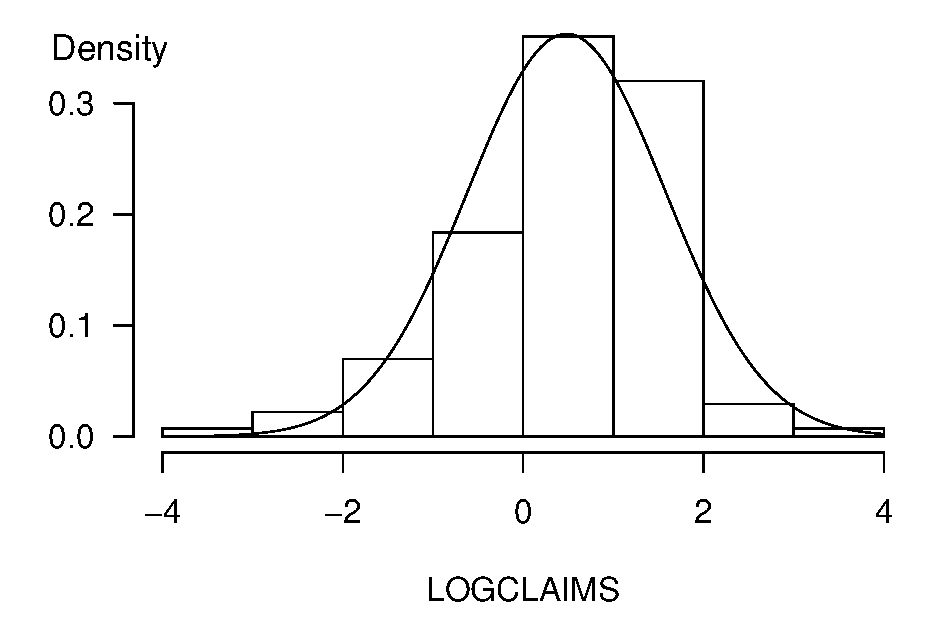
\includegraphics[width=0.45\textwidth]
        {Chapter1/F1BIHist.eps} \hfill  $~~~$
               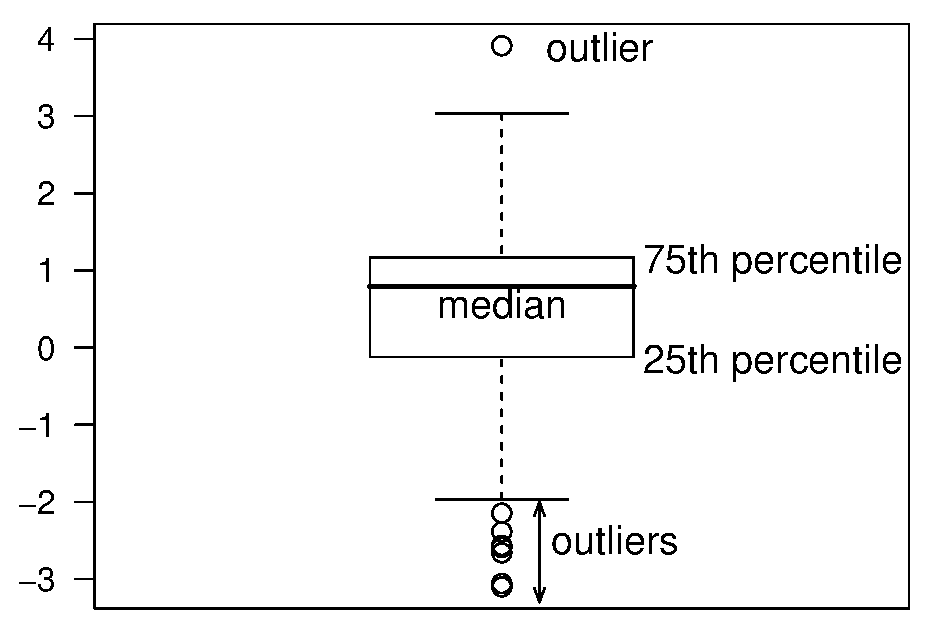
\includegraphics[width=0.45\textwidth]
        {Chapter1/F1BoxPlot.eps}

      \parbox[t]{2.5in}{\caption{\label{F1:BIHist} \small Bodily Injury Relative Frequency with Normal Curve
                Superimposed.}} \hfill
        \parbox[t]{2.5in}{\caption{\label{F1:BoxPlot} \small Box Plot of Bodily Injury
        Claims.}}
\end{figure}


\bigskip\index{plots!box and whiskers}

\textbf{Box Plot. \ }A quick visual inspection of a variable's
distribution can reveal some surprising features that are hidden by
statistics, numerical summary measures. The \emph{box plot}
\index{plots!box}, also known as a ``box and whiskers'' plot, is one
such graphical device. Figure \ref{F1:BoxPlot} illustrates a box
plot for the bodily injury claims. Here, the box captures the middle
50\% of the data, with the three horizontal lines corresponding to
the 75th, 50th and 25th percentiles, reading from top to bottom. \
The horizontal lines above and below the box are the ``whiskers.''
The upper whisker is 1.5 times the \emph{interquartile range} (the
difference between the 75th and 25th percentiles) above the 75th
percentile. Similarly, the lower whisker is 1.5 times the
interquartile range below the 25th percentile. Individual
observations outside the whiskers are denoted by small circular
plotting symbols, and are referred to as ``outliers.''

\bigskip

Graphs are powerful tools; they allow analysts to readily visualize
nonlinear relationships that are hard to comprehend when expressed
verbally or by mathematical formula. However, by their very
flexibility, graphs can also readily deceive the analyst. Chapter 21
will underscore this point. For example, Figure
\ref{F1:BIHistRedraw} is a re-drawing of Figure \ref{F1:BIHist}; the
difference is that Figure \ref{F1:BIHistRedraw} uses more, and
finer, rectangles. This finer analysis reveals the asymmetric nature
of the sample distribution that was not evident in Figure
\ref{F1:BIHist}.


\bigskip

\textbf{Quantile-Quantile Plots.} Increasing the number of
rectangles can unmask features that were not previously apparent;
however, there are in general fewer observations per rectangle
meaning that the uncertainty of the relative frequency estimate
increases. This represents a trade-off. Instead of forcing the
analyst to make an arbitrary decision about the number of
rectangles, an alternative is to use a graphical device for
comparing a distribution to another known as a
\emph{quantile-quantile}, or \emph{qq},
plot.\index{plots!quantile-quantile, $qq$}

Figure \ref{F1:BIQQPlot} illustrates a $qq$ plot for the bodily
injury data using the normal curve as a reference distribution. For
each point, the vertical axis gives the quantile using the sample
distribution. The horizontal axis gives the corresponding quantity
using the normal curve. For example, earlier we considered the 75th
percentile point. This point appears as (1.168, 0.675) on the graph.
To interpret a $qq$ plot, if the quantile points lie along the
superimposed line, then the sample and the normal reference
distribution have the same shape. (This line is defined by
connecting the 75th and 25th percentiles.)

\marginparjed{Points in a $qq$ plot close to a straight line
suggests agreement between the sample and reference distributions.}

In Figure \ref{F1:BIQQPlot}, the small sample percentiles are
consistently smaller than the corresponding values from the standard
normal, indicating that the distribution is skewed to the left. The
difference in values at the ends of the distribution are due to the
outliers noted earlier that could also be interpreted as the sample
distribution having larger tails than the normal reference
distribution.




\begin{figure}[htp]
  \begin{center}
    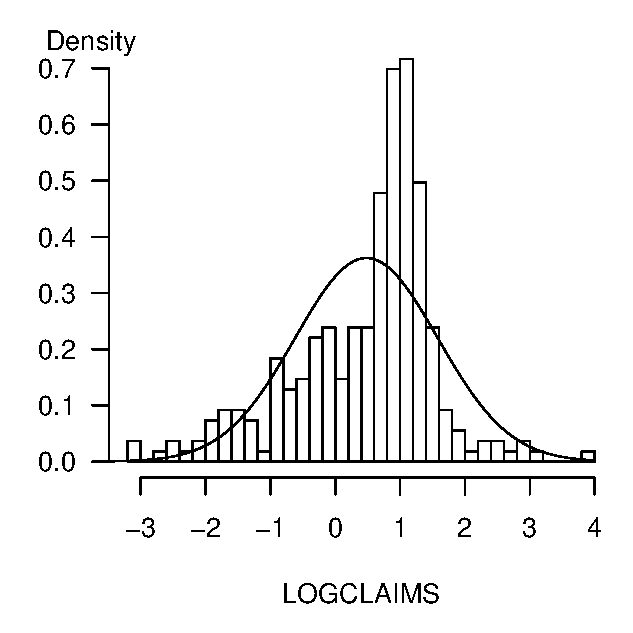
\includegraphics[width=0.45\textwidth]
        {Chapter1/F1BIHistRedraw.eps}
      \hfill
            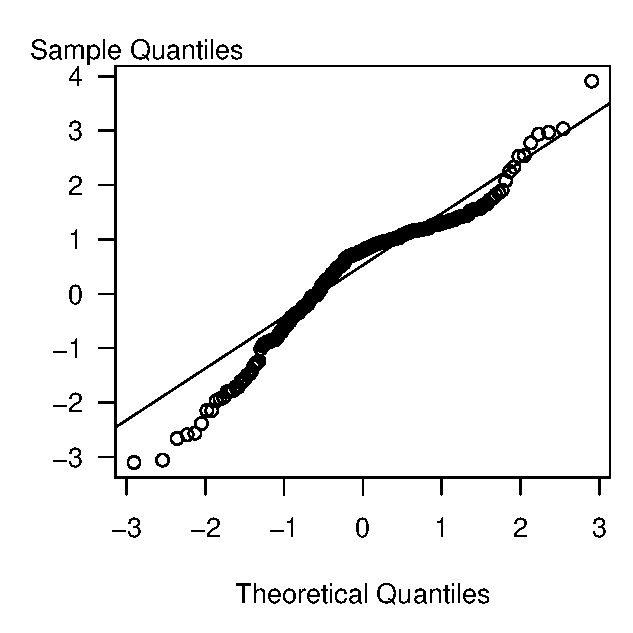
\includegraphics[width=0.45\textwidth]
        {Chapter1/F1BIQQPlot.eps}

      \end{center}
           \parbox[t]{2.5in}{\caption {\label{F1:BIHistRedraw}
           {\small Re-drawing of Figure \ref{F1:BIHist} with an increased number of rectangles.}}} \hfill
        \parbox[t]{2.5in}{\caption {\label{F1:BIQQPlot} {\small A $qq$ plot of
Bodily Injury Claims, using a normal reference distribution.}}}

\end{figure}


\section{Power Transforms}\label{S1:PowerTransforms}\index{transformations!power}

In the Section 1.2 example, we considered claims without justifying
the use of the logarithmic scaling. When analyzing variables such as
assets of firms, wages of individuals and housing prices of
households in business and economic applications, it is common to
consider logarithmic instead of the original units. A log transform
retains the original ordering (for example, large wages remain large
on the log wage scale) but serves to ``pull in'' extreme values of
the distribution.

To illustrate, Figure \ref{F1:BIOrig} shows the bodily injury claims
distribution in (thousands of) dollars. In order to graph the data
meaningfully, the largest observation (\$50,000) was removed prior
to making this plot. Even with this observation removed, Figure
\ref{F1:BIOrig} shows that the distribution is heavily lop-sided to
the right, with several large values of claims appearing.
\index{transformations!logarithmic}


\marginparjed{A right-skewed distribution is has long tails on the
right and a concentration of mass on the left. Many insurance claims
distributions are right-skewed.}

Distributions that are lopsided in one direction or the other are
known as \emph{skewed}. Figure \ref{F1:BIOrig} is an example of a
distribution skewed to the right, or positively skewed. Here, the
tail of the distribution on the right is longer and there is a
greater concentration of mass to the left. In contrast, a
left-skewed, or negatively skewed distribution, has a longer tail on
the left and a greater concentration of mass to the right. Many
insurance claims distributions are right-skewed (see the text by
Klugman, Panjer and Willmot, 2008, for extensive discussions). As we
saw in Figures \ref{F1:BIHistRedraw} and \ref{F1:BIQQPlot}, a
logarithmic transformation yields a distribution that is only mildly
skewed to the left.


\setcounter{figure}{5}

\begin{figure}[htp]
  \begin{center}
    
\includegraphics[width=.4\textwidth]
        {Chapter1/F1BIOrig.eps}
    \caption{\label{F1:BIOrig} \small Distribution of Bodily Injury Claims. Observations are in (thousands of)
dollars with the largest observation omitted.}
  \end{center}
\end{figure}

\index{transformations!Box-Cox family}

Logarithmic transformations are used extensively in applied
statistics work. One advantage is that they serve to symmetrize
distributions that are skewed. More generally, we consider
\emph{power transforms}, also known as the \emph{Box-Cox family of
transforms}. Within this family of transforms, in lieu of using the
response $y$, we use a transformed, or rescaled version, $y^{\lambda
}$. Here, the power $\lambda $ (lambda, a Greek ``el'') is a number
that may be user specified. Typical values of $\lambda $ that are
used in practice are $\lambda $=1, 1/2, 0 or -1. When we use
$\lambda =0$, we mean $\ln (y)$, that is, the natural logarithmic
transform. More formally, the Box-Cox family can be expressed as
\begin{equation*}
y^{(\lambda )}=\left\{
\begin{array}{ll}
\frac{y^{\lambda }-1}{\lambda } & \lambda \neq 0 \\
\ln (y) & \lambda =0
\end{array}
\right. .
\end{equation*}
As we will see, because regression estimates are not affected by
location and scale shifts, in practice we do not need to subtract
one nor divide by $\lambda $ when rescaling the response. The
advantage of the above expression is that, if we let $\lambda $
approach 0, then $y^{(\lambda )}$ approaches $\ln (y)$, from some
straightforward calculus arguments.

To illustrate the usefulness of transformations, we simulated 500
observations from a chi-square distribution with two degrees of
freedom. Appendix A3.2 introduces this distribution (that we will
encounter again later in studying the behavior of test statistics).
The upper left panel of Figure \ref{F1:ChiSquare} shows the original
distribution is heavily skewed to the right. The other panels in
Figure \ref{F1:ChiSquare} show the data rescaled using the square
root, logarithmic and negative reciprocal transformations. The
logarithmic transformation, in the lower left panel, provides the
best approximation to symmetry for this example. The negative
reciprocal transformation is based on $\lambda =-1$, and then
multiplying the rescaled observations by minus one, so that large
observations remain large.\index{distributions!chi-square}


\begin{figure}[htp]
  \begin{center}
    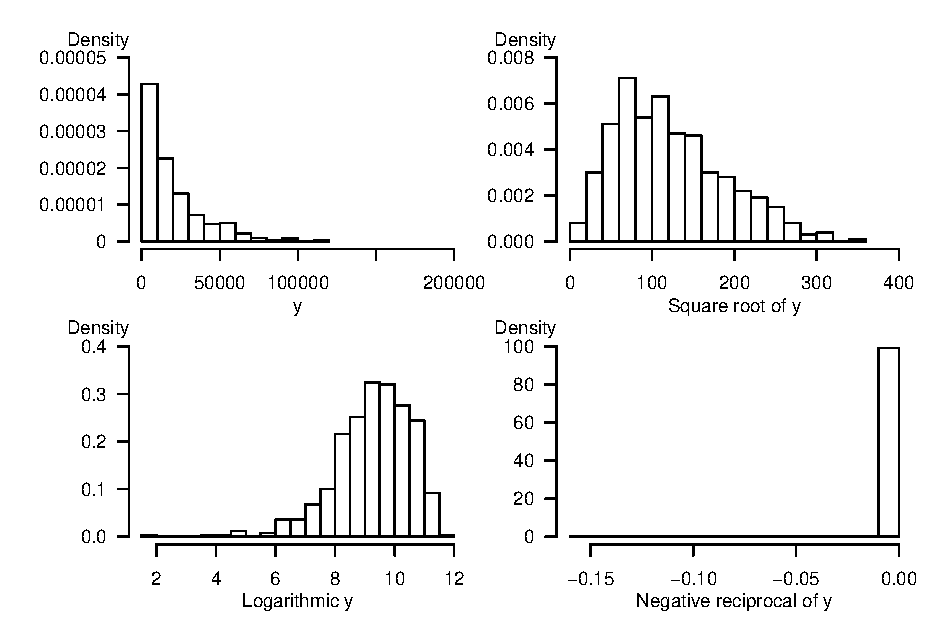
\includegraphics[width=1\textwidth]
        {Chapter1/F1Chisquare.eps}
    \caption{\label{F1:ChiSquare} \small 500
simulated observations from a chi-square distribution. The upper
left panel is based on the original distribution. The upper right
corresponds to the square root transform, the lower left to the log
transform and the lower right to the negative reciprocal transform.}
  \end{center}
\end{figure}


\section{Sampling and the Role of Normality}

\index{statistic}

A \emph{statistic} is a summary measure of data, such as a mean,
median or percentile. Collections of statistics are very useful for
analysts, decision-makers and everyday consumers for understanding
massive amounts of data that represent complex situations. To this
point, our focus has been on introducing sensible techniques to
summarize variables; techniques that will be used repeatedly thought
this text. However, the true usefulness of the \emph{discipline of
statistics} is its ability to say something about the unknown, not
merely to summarize information already available. To this end, we
need to make some fairly formal assumptions about the manner in
which the data are observed. As a science, a strong feature of
statistics (as a discipline) is the ability to critique these
assumptions and offer improved alternatives in specific situations.

\marginparjed{A statistic is a summary measure of a sample.
Statistics, as a discipline, can be used to infer behavior about a
larger population from a sample.}

\index{model assumptions}\index{symbols!$\mu$, population mean}
\index{symbols!$\sigma^2$, population
variance}\index{symbols!$\sigma$, population standard deviation}
\index{symbols!E , expectation operator}\index{symbols!Var ,
variance operator}

It is customary to assume that the data are drawn from a larger
population that we are interested in describing. The process of
drawing the data is known as the \emph{sampling}, or \emph{data
generating, process}. We denote this sample as $\{y_1,\ldots,y_n\}$.
So that we may critique, and modify, these sampling assumptions, we
list them below in detail:\smallskip

\begin{center}
\begin{tabular}{l}
\hline \textit{Basic Sampling Assumptions} \\ \hline
1. $\mathrm{E~}y_i=\mu $ \\
2. $\mathrm{Var~}y_i=\sigma ^{2}$ \\
3. $\{y_i\}$ are independent \\
4. $\{y_i\}$ are normally distributed. \\ \hline
\end{tabular}
\end{center}

\marginparjed{Assumption 4 is not required for many statistical
inference procedures because central limit theorems provide
approximate normality for many statistics of interest.}

In this basic set-up, $\mu $\ and $\sigma ^{2}$\ serve as
\emph{parameters} that describe the location and scale of the parent
population. The goal is to infer something sensible about them based
on statistics such as $\overline{y}$ and $s_y^{2}$. For the third
assumption, we assume independence among the draws. In a sampling
scheme, this may be guaranteed by taking a simple random sample from
a population. The fourth assumption is not required for many
statistical inference procedures because central limit theorems
provide approximate normality for many statistics of interest.
However, a formal justification of some statistics, such as
\textit{t}-statistics, requires this additional
assumption.\index{theorems!central limit}

Section \ref{S1:TechSupp} provides an explicit statement of one
version of the central limit theorem, giving conditions under which
$\overline{y}$ is approximately normally distributed. This section
also discusses a related result, known as an \emph{Edgeworth
approximation}, that shows that the quality of the normal
approximation is better for symmetric parent populations when
compared to skewed distributions.

\marginparjed{Linear regression is the study of weighted averages.}

How does this discussion apply to the study of regression analysis?
After all, so far we have focused only on the simple arithmetic
average, $\overline{y}$. In subsequent chapters, we will emphasize
that \emph{linear regression is the study of weighted averages};
specifically, many regression coefficients can be expressed as
weighted averages with appropriately chosen weights. Central limit
and Edgeworth approximation theorems are available for weighted
averages - these results will ensure approximate normality of
regression coefficients. To use normal curve approximations in a
regression context, we will often transform variables to achieve
approximate symmetry.

\marginparjed{We often transform variables to achieve approximate
symmetry to use normal curve approximations in a regression
context.}

\section{Regression and Sampling Designs}

Approximating normality will be an important issue in practical
applications of linear regression. Parts I and II of this book focus
on linear regression, where we will learn basic regression concepts
and sampling design. Part III will focus on \emph{nonlinear}
regression, involving binary, count and fat-tailed responses, where
the normal is not the most helpful reference distribution. Ideas
concerning basic concepts and design will also be used in the
nonlinear setting.

In regression analysis, we focus on one measurement of interest and
call this the \emph{dependent variable}. Other measurements are used
as \emph{explanatory variables}. A goal is to compare differences in
the dependent variable in terms of differences in the explanatory
variables. As noted in Section \ref{S1:Intro}, regression is used
extensively in many scientific fields. Table
\ref{T1:RegressionTerms} lists alternative terms that you may
encounter as you read regression applications.

\index{explanatory variable!independent variable}\index{explanatory
variable!regressor}\index{explanatory
variable!predictor}\index{explanatory variable!right-hand side}
\index{explanatory variable!exogenous}

\index{dependent variable}\index{dependent variable!outcome of
interest}\index{dependent variable!endogenous}\index{dependent
variable!response}\index{dependent
variable!regressand}\index{dependent variable!left-hand
side}\index{dependent variable!explained}

\begin{table}[h] \scalefont{0.9}
\caption{\label{T1:RegressionTerms} Terminology for Regression
Variables}
\begin{tabular}{ll}
\hline \multicolumn{1}{c}{$y$-variable} & \multicolumn{1}{c}{$x$-variable} \\
Outcome of interest & Explanatory variable \\
Dependent variable & Independent variable \\
Endogenous variable & Exogenous variable \\
Response & Treatment \\
Regressand & Regressor \\
Left-hand side variable & Right-hand side variable \\
Explained variable & Predictor variable \\
Output & Input \\
 \hline
\end{tabular}\scalefont{1.1111}\end{table}



In the latter part of the nineteenth century and early part of the
twentieth century, statistics was beginning to make an important
impact on the development of experimental science. Experimental
sciences often use \emph{designed studies}, where the data are under
the control of an analyst. Designed studies are performed in
laboratory settings, where there are tight physical restrictions on
every variable that a researcher thinks may be important. Designed
studies also occur in larger field experiments, where the mechanisms
for control are different than in laboratory settings. Agriculture
and medicine use designed studies. Data from a designed study are
said to be \emph{experimental data}.

\marginparjed{In designed studies, the data are under the control of
an analyst. Data from a designed study are said to be experimental
data.}

To illustrate, a classic example is to consider the yield of a crop
such as corn, where each of several parcels of land (the
observations) are assigned various levels of fertilizer. The goal is
ascertain the effect of fertilizer (the explanatory variable) on the
corn yield (the response variable). Although researchers attempt to
make parcels of land as much alike as possible, differences
inevitably arise. Agricultural researchers use \emph{randomization
techniques} to assign different levels of fertilizer to each parcel
of land. In this way, analysts can explain the variation in corn
yields in terms of the variation of fertilizer levels. Through the
use of randomization techniques, researchers using designed studies
can infer that the treatment has a \emph{causal effect} on the
response. Chapter 6 discusses causality further.

\linejed \index{examples!Rand health insurance
experiment}\index{actuarial \& financial terms and concepts!demand}

\textbf{Example: Rand Health Insurance Experiment}. How are medical
care expenditures related to the demand for insurance? Many studies
have established a positive relation between the amount spent on
medical care and the demand for health insurance. Those in poor
health anticipate using more medical services than similarly
positioned people in good or fair health and will seek higher levels
of health insurance to compensate for these anticipated
expenditures. They obtain this additional health insurance by (i)
selecting a more generous health insurance plan from an employer,
(ii) choosing an employer with a more generous health insurance plan
or (iii) paying more for individual health insurance. Thus, it is
difficult to disentangle the cause and effect relationship of
medical care expenditures and the availability of health insurance.

A study reported by Manning et al. (1987) sought to answer this
question using a carefully designed experiment. In this study,
enrolled households from six cities, between November 1974 and
February 1977, were \emph{randomly assigned} to one of 14 different
insurance plans. These plans varied by the cost-sharing elements,
the co-insurance rate (the percentage paid on out-of-pocket
expenditures which varied by 0, 25, 50 and 95\%) as well as the
deductible (5, 10 or 15 percent of family income, up to a maximum of
\$1,000). Thus, there was a \emph{random} assignment to levels of
the treatment, the amount of health insurance. The study found that
more favorable plans resulted in greater total expenditures, even
after controlling for participants' health status.

\linejed

\bigskip

For actuarial science and other social sciences, designed studies
are the exception rather than the rule. For example, if we want to
study the effects of smoking on mortality, it is highly unlikely
that we could get study participants to agree to be randomly
assigned to smoker/nonsmoker groups for several years just so that
we could observe their mortality patterns! As with the Section
\ref{S1:Intro} Galton study, social science researchers generally
work with \emph{observational data}. Observational data are not
under control of the analyst.

With observational data, we can not infer causal relationships but
we can readily introduce measures of \emph{association}. To
illustrate, in the Galton data, it is apparent that ``tall'' parents
are likely to have ``tall'' children and conversely ``short''
parents are likely to have ``short'' children. Chapter 2 will
introduce a correlation and other measures of association. However,
we can not infer causality from the data. For example, there may be
another variable, such as family diet, that is related to both
variables. Good diet in the family could be associated with tall
heights of parents and adult children, whereas poor diet stifles
growth. If this were the case, we would call family diet a
\emph{confounding variable}.

\marginparjed{With statistical control, we seek to compare a $y$ and
an $x$, ``controlling for'' the effects of other explanatory
variables.}

In designed experiments such as the Rand Health Insurance
Experiment, we can control for the effects of variables such as
health status through random assignment methods. In observational
studies, we use \emph{statistical control}, rather than experimental
control. To illustrate, for the Galton data, we might split our
observations into two groups, one for ``good family diet'' and one
for ``poor family diet,'' and examine the relationship between
parents' and children's height for each subgroup. This is the
essence of the regression method, to compare a $y$ and an $x$,
``controlling for'' the effects of other explanatory variables.

Of course, to use statistical control and regression methods, one
must record family diet, and any other measures of height that may
confound the effects of parents' height on the height of their adult
child. The difficulty in designing studies is trying to imagine all
of the variables that could possibly affect a response variable, an
impossible task in most social science problems of interest. To give
some guidance on when ``enough is enough,'' Chapter 6 will discuss
measures of an explanatory variable's importance and its impact on
model selection.

\section{Actuarial Applications of Regression}

This book introduces a statistical method, regression analysis. The
introduction is organized around the traditional triad of
statistical inference:
\begin{itemize}
\item hypothesis testing,
\item estimation and
\item prediction.
\end{itemize}
Further, this book shows how this methodology can be used in
applications that are likely to be of interest to actuaries and to
other risk analysts. As such, it is helpful to begin with the three
traditional areas of actuarial applications:
\begin{itemize}
\item pricing,
\item reserving and
\item solvency testing.
\end{itemize}

\index{actuarial \& financial terms and concepts!adverse selection}
\index{actuarial \& financial terms and concepts!pricing}

\textbf{Pricing and adverse selection.} Regression analysis can be
used to determine insurance prices for many lines of business. For
example, in private passenger automobile insurance, expected claims
vary by the insured's gender, age, location (city versus rural),
vehicle purpose (work or pleasure) and a host of other explanatory
variables. Regression can be used to identify the variables that are
important determinants of expected claims.

In competitive markets, insurance companies do not use the same
price for all insureds. If they did, ``good risks,'' those with
lower than average expected claims, would overpay and leave the
company. In contrast, ``bad risks,'' those with higher than average
expected claims, would remain with the company. If the company
continued this flat rate pricing policy, premiums would rise (to
compensate for claims by the increasing share of bad risks) and
market share would dwindle as the company loses good risks. This
problem is known as ``adverse selection.'' Using an appropriate set
of explanatory variables, classification systems can be developed so
that each insured pays their fair share.

\index{actuarial \& financial terms and concepts!reserve}
\index{actuarial \& financial terms and concepts!solvency testing}

\textbf{Reserving and solvency testing.} Both reserving and solvency
testing are concerned with predicting whether liabilities associated
with a group of policies will exceed the capital devoted to meeting
obligations arising from the policies. Reserving involves
determining the appropriate amount of capital to meet these
obligations. Solvency testing is about assessing the adequacy of
capital to fund the obligations for a block of business. In some
practice areas, regression can be used to forecast future
obligations to help determine reserves (see, for example, Chapter
19). Regression can also be used to compare characteristics of
healthy and financially distressed firms for solvency testing (see,
for example, Chapter 14).


\textbf{Other risk management applications.} Regression analysis is
a quantitative tool that can be applied in a broad variety of
business problems, not just the traditional areas of pricing,
reserving and solvency testing. By becoming familiar with regression
analysis, actuaries will have another quantitative skill that can be
brought to bear on general problems involving the financial security
of people, companies and governmental organizations. To help you
develop insights, this book provides many examples of potential
``non-actuarial'' applications through featured vignettes labeled as
``examples'' and illustrative data sets.

To help understand potential regression applications, start by
reviewing the several data sets featured in the Chapter 1 Exercises.
Even if you do not complete the exercises to strengthen your data
summary skills (that require the use of a computer), a review of the
problem descriptions will help you become more familiar with types
of applications in which an actuary might use regression techniques.




\section{Further Reading and References}


This book introduces regression and time series tools that are most
relevant to actuaries and other financial risk analysts.
Fortunately, there are other sources that provide excellent
introductions to these statistical topics (although not from a risk
management viewpoint). Particularly for analysts that intend to
specialize in statistics, it is helpful to get another perspective.
For regression, I recommend Weisburg (2005) and Faraway (2005). For
time series, Diebold (2004) is a good source. Moreover, Klugman,
Panjer and Willmot (2008) provides a good introduction to actuarial
applications of statistics; this book is intended to complement the
Klugman et al. book by focusing on regression and time series
methods.

\bigskip

\textbf{Chapter References}

\begin{multicols}{2}

\scalefont{0.9}

Beard, Robert E.,  Teivo Pentik\"{a}inen and Erkki Pesonen (1984).
\textit{Risk Theory: The Stochastic Basis of Insurance} (Third
Edition). Chapman \& Hall, New York.

Diebold, Francis. X. (2004). \textit{Elements of Forecasting, Third
Edition.} Thomson, South-Western, Mason, Ohio.

Faraway, Julian J. (2005). \textit{Linear Models in R.} Chapman \&
Hall/CRC, New York.

Hogg, Robert V. (1972). On statistical education. \textit{The
American Statistician} 26, 8-11.

Klugman, Stuart A, Harry H. Panjer and Gordon E. Willmot (2008).
\emph{Loss Models: From Data to Decisions}. John Wiley \& Sons,
Hoboken, New Jersey.

Manning, Willard G., Joseph P. Newhouse, Naihua Duan, Emmett B.
Keeler, Arleen Leibowitz and M. Susan Marquis (1987). Health
insurance and the demand for medical care: Evidence from a
randomized experiment. \textit{American Economic Review} 77, No. 3,
251-277.

Rempala, Grzegorz A. and Richard A. Derrig (2005). Modeling hidden
exposures in claim severity via the EM algorithm. \textit{North
American Actuarial Journal} 9, No. 2, 108-128.

Singer, Judith D. and Willett, J. B. (1990). Improving the teaching
of applied statistics:  Putting the data back into data analysis.
\textit{The American Statistician} 44, 223-230.

Stigler, Steven M. (1986). \textit{The History of Statistics:  The
Measurement of Uncertainty before 1900}. The Belknap Press of
Harvard University Press, Cambridge, MA.

Weisberg, Sanford (2005). \textit{Applied Linear Regression, Third
Edition.} John Wiley \& Sons, New York.


\scalefont{1.1111}

\end{multicols}

\section{Exercises}

\scalefont{0.90}


\begin{exercises}
\empexjed{HealthExpend}\index{datasets!MEPS health expenditures}

\item \textbf{MEPS health expenditures.}\label{Ex:MedExpend} This exercise considers data
from the Medical Expenditure Panel Survey (MEPS), conducted by the
U.S. Agency of Health Research and Quality. MEPS is a probability
survey that provides nationally representative estimates of health
care use, expenditures, sources of payment, and insurance coverage
for the U.S. civilian population. This survey collects detailed
information on individuals of each medical care episode by type of
services including physician office visits, hospital emergency room
visits, hospital outpatient visits, hospital inpatient stays, all
other medical provider visits, and use of prescribed medicines. This
detailed information allows one to develop models of health care
utilization to predict future expenditures. You can learn more about
MEPS at http://www.meps.ahrq.gov/mepsweb/.

We consider MEPS data from the panels 7 and 8 of 2003 that consists
of 18,735 individuals between ages 18 and 65. From this sample, we
took a random sample of 2,000 individuals that appear in the file
``HealthExpend''. From this sample, there are 157 individuals that
had positive inpatient expenditures. There are also 1,352 that had
positive outpatient expenditures. We will analyze these two samples
separately.

Our dependent variables consist of amounts of expenditures for
inpatient (EXPENDIP) and outpatient (EXPENDOP) visits. For MEPS,
outpatient events include hospital outpatient department visits,
office-based provider visits and emergency room visits excluding
dental services. (Dental services, compared to other types of health
care services, are more predictable and occur in a more regular
basis.) Hospital stays with the same date of admission and
discharge, known as ``zero-night stays,'' were included in
outpatient counts and expenditures. (Payments associated with
emergency room visits that immediately preceded an inpatient stay
were included in the inpatient expenditures. Prescribed medicines
that can be linked to hospital admissions were included in inpatient
expenditures, not in outpatient utilization.)

Part 1: Use only the 157 individuals that had positive inpatient
expenditures and do the following analysis.

a. Compute descriptive statistics for inpatient (EXPENDIP)
expenditures.

a(i) What is the typical (mean and median) expenditure?

a(ii) How does the standard deviation compare to the mean? Do the
data appear to be skewed?

b. Compute a box plot, histogram and a (normal) $qq$ plot for
EXPENDIP. Comment on the shape of the distribution.

c. Transformations.

c(i) Take a square root transform of inpatient expenditures.
Summarize the resulting distribution using a histogram and a $qq$
plot. Does it appear to be approximately normally distributed?

c(ii). Take a (natural) logarithmic transformation of inpatient
expenditures. Summarize the resulting distribution using a histogram
and a $qq$ plot. Does it appear to be approximately normally
distributed?

Part 2: Use only the 1,352 individuals that had positive outpatient
expenditures.

d. Repeat part (a) and compute histograms for expenditures and
logarithmic expenditures. Comment on the approximate normality for
each histogram.

\empexjed{WiscNursingHome}\index{datasets!nursing home utilization}

\item \textbf{Nursing Home Utilization.}\label{Ex:NursHome}
This exercise considers nursing home data provided by the Wisconsin
Department of Health and Family Services (DHFS). The State of
Wisconsin Medicaid program funds nursing home care for individuals
qualifying on the basis of need and financial status. As part of the
conditions for participation, Medicaid-certified nursing homes must
file an annual cost report to DHFS, summarizing the volume and cost
of care provided to all of its residents, Medicaid-funded and
otherwise. These cost reports are audited by DHFS staff and form the
basis for facility-specific Medicaid daily payment rates for
subsequent periods. The data are publicly available; see
\texttt{http://dhfs.wisconsin.gov/provider}
\texttt{/prev-yrs-reports-nh.htm} for more information.

The DHFS is interested in predictive techniques that provide
reliable utilization forecasts to update their Medicaid funding rate
schedule of nursing facilities. In this assignment, we consider the
data in the file ``WiscNursingHome'' in cost report years 2000 and
2001. There are 362 facilities in 2000 and 355 facilities in 2001.
Typically, utilization of nursing home care is measured in patient
days (``patient days'' is the number of days each patient was in the
facility, summed over all patients). For this exercise, we define
the outcome variable to be total patient years (TPY), the number of
total patient days in the cost reporting period divided by number of
facility operating days in the cost reporting period (see Rosenberg
et al., 2007, Appendix 1, for further discussion of this choice).
The number of beds (NUMBED) and square footage (SQRFOOT) of the
nursing home both measure the size of the facility. Not
surprisingly, these continuous variables will be important
predictors of TPY.

\textbf{Part 1:} Use cost report year 2000 data, and do the
following analysis.

a. Compute descriptive statistics for TPY, NUMBED, and SQRFOOT.

b. Summarize the distribution of TPY using a histogram and a $qq$
plot. Does it appear to be approximately normally distributed?

c. Transformations. Take a (natural) logarithmic transformation of
TPY (LOGTPY). Summarize the resulting distribution using a histogram
and a $qq$ plot. Does it appear to be approximately normally
distributed?


\textbf{Part 2:} Use cost report year 2001 data and repeat parts (a)
and (c).

\empexjed{AutoClaims}\index{datasets!automobile insurance claims}

\item \textbf{Automobile Insurance Claims.}\label{Ex:AutoClaims} As an actuarial analyst,
you are working with a large insurance company to help them
understand their claims distribution for their private passenger
automobile policies. You have available claims data for a recent
year, consisting of:

\begin{itemize}
\item STATE CODE: codes 01 through 17 used, with each code randomly
assigned to an actual individual state

\item CLASS: rating class of operator, based on age, gender, marital
status and use of vehicle

\item GENDER:  operator gender AGE: operator age

\item PAID: amount paid to settle and close a claim.

You are focusing on older drivers, 50 and higher, for which there
are $n = 6,773$ claims available.

\end{itemize}

Examine the histogram of the amount PAID and comment on the
symmetry. Create a new variable, the (natural) logarithmic claims
paid, LNPAID. Create a histogram and a $qq$ plot of LNPAID. Comment
on the symmetry of this variable.

\empexjed{HospitalCosts}\index{datasets!hospital costs}

\item \textbf{Hospital Costs.}\label{Ex:HospExpend} Suppose
that you are an employee benefits actuary working with a medium size
company in Wisconsin. This company is considering offering, for the
first time in their industry, hospital insurance coverage to
dependent children of their employees. You have access to company
records and so have available the number, age and gender of the
dependent children but have no other information about hospital
costs from the company. In particular, no firm in this industry has
offered this coverage and so you have little historical industry
experience upon which you can forecast expected claims.

You gather data from the Nationwide Inpatient Sample of the
Healthcare Cost and Utilization Project (NIS-HCUP), a nationwide
survey of hospital costs conducted by the US Agency for Healthcare
Research and Quality (AHRQ). You restrict consideration to Wisconsin
hospitals and analyze a random sample of $n=500$ claims from 2003
data. Although the data comes from hospital records, it is organized
by individual discharge and so you have information about the age
and gender of the patient discharged. Specifically, you consider
patients aged 0-17 years. In a separate project, you will consider
the frequency of hospitalization. For this project, the goal is to
model the severity of hospital charges, by age and gender.

a. Examine the distribution of the dependent variable, TOTCHG. Do
this by making a histogram and then a $qq$ plot, comparing the
empirical to a normal distribution.

b. Take a natural log transformation and call the new variable
LNTOTCHG. Examine the distribution of this transformed variable. To
visualize the logarithmic relationship, plot LNTOTCHG versus TOTCHG.

\newpage

\empexjed{AutoBI}\index{datasets!automobile injury insurance
claims}\index{actuarial \& financial terms and concepts!closed
claim}

\item \textbf{Automobile injury insurance claims.}\label{Ex:IRC}
We consider automobile injury claims data using data from the
Insurance Research Council (IRC), a division of the American
Institute for Chartered Property Casualty Underwriters and the
Insurance Institute of America. The data, collected in 2002,
contains information on demographic information about the claimant,
attorney involvement and the economic loss (LOSS, in thousands),
among other variables. We consider here a sample of $n=1,340$ losses
from a single state. The full 2002 study contains over 70,000 closed
claims based on data from thirty-two insurers. The IRC conducted
similar studies in 1977, 1987, 1992 and 1997.

a. Compute descriptive statistics for the total economic loss
(LOSS). What is the typical loss?

b. Compute a histogram and (normal) $qq$ plot for LOSS. Comment on
the shape of the distribution.

c. Partition the data set into two subsamples, one corresponding to
those claims that involved an ATTORNEY (=1) and the other where an
ATTORNEY was not involved (=2).

c(i). For each subsample, compute the typical loss. Does there
appear to be a difference in the typical losses by attorney
involvement?

c(ii) To compare the distributions, compute a boxplot by level of
attorney involvement.

c(iii). For each subsample, compute a histogram and $qq$ plot.
Compare the two distributions to one another.


\empexjed{NAICExpense}\index{datasets!insurance company expenses}

\item  \textbf{Insurance Company Expenses.}\label{Ex:NAICExpense}
Like other businesses, insurance companies seek to minimize expenses
associated with doing business in order to enhance profitability. To
study expenses, this exercise examines a random sample of 500
insurance companies from the National Association of Insurance
Commissioners (NAIC) database of over 3,000 companies. The NAIC
maintains one of the world's largest insurance regulatory databases;
we consider here data that are based on 2005 annual reports for all
the property and casualty insurance companies in the United States.
The annual reports are financial statements that use statutory
accounting principles.

Specifically, our dependent variable is EXPENSES, the non-claim
expenses for a company. Although not needed for this exercise,
non-claim expenses are based on three components: unallocated loss
adjustment, underwriting and investment expenses. The unallocated
loss adjustment expense is the expense not directly attributable to
a claim but is indirectly associated with settling claims; it
includes items such as the salaries of claims adjusters, legal fees,
court costs, expert witnesses and investigation costs. Underwriting
expenses consists of policy acquisition costs, such as commissions,
as well as the portion of administrative, general and other expenses
attributable to underwriting operations. Investment expense are
those expenses related to investment activities of the insurer.

a. Examine the distribution of the dependent variable, EXPENSES. Do
this by making a histogram and then a $qq$ plot, comparing the
empirical to a normal distribution.

b. Take a natural log transformation and examine the distribution of
this transformed variable. Has the transformation helped to
symmetrize the distribution?


\empexjed{UNLifeExpectancy}\index{datasets!national life
expectancies}

\item \textbf{National Life Expectancies.}\label{Ex:UNLIFE} Who is doing health care right?
Health care decisions are made at the individual, corporate and
government levels. Virtually every person, corporation and
government have their own perspective on health care; these
different perspectives result in a wide variety of systems for
managing health care. Comparing different health care systems help
us learn about approaches other than our own, which in turn help us
make better decisions in designing improved systems.

Here, we consider health care systems from $n=185$ countries
throughout the world. As a measure of the quality of care, we use
LIFEEXP, the life expectancy at birth. This dependent variable, with
several explanatory variables, are listed in Table
\ref{Ex:UNLIFESummStats}. From this table, you will note that
although there are 185 countries consider in this study, not all
countries provided information for each variable. Data not available
are noted under the column ``Num Miss.'' The data are from the
United Nations (UN) Human Development Report.

a. Examine the distribution of the dependent variable, LIFEEXP. Do
this by making a histogram and then a $qq$ plot, comparing the
empirical to a normal distribution.

b. Take a natural log transformation and examine the distribution of
this transformed variable. Has the transformation helped to
symmetrize the distribution?



\begin{table}[h]
\scalefont{0.8} \caption{\label{Ex:UNLIFESummStats} \small Life
Expectancy, Economic and Demographic Characteristics of 185
Countries}
\begin{tabular}{ll|crrrrr}
\hline
&  & Num &        &     & Standard  &   Mini- &  Maxi- \\
  Variable     & Description & Miss &    Mean    &    Median   & Deviation &    mum &    mum \\\hline
BIRTH & Births attended  by skilled &          7 &      78.25 &      92.00 &      26.42 &       6.00 &     100.00 \\
 ~~ATTEND& ~~ health personnel (\%)\\
FEMALE & Legislators, senior officials &         87 &      29.07 &      30.00 &      11.71 &       2.00 &      58.00 \\
 ~~BOSS& ~~ and managers, \% female \\
 FERTILITY & Total fertility rate,&          4 &       3.19 &       2.70 &       1.71 &       0.90 &       7.50 \\
 & ~~ births per woman &          \\
       GDP & Gross domestic product, &          7 &     247.55 &      14.20 &   1,055.69 &       0.10 &  12,416.50 \\
       & ~~in billions of USD \\
HEALTH& 2004 Health expenditure &          5 &     718.01 &     297.50 &   1,037.01 &      15.00 &   6,096.00 \\
~~ EXPEND & ~~ per capita, PPP in USD \\
ILLITERATE & Adult illiteracy rate,  &         14 &      17.69 &      10.10 &      19.86 &       0.20 &      76.40 \\
  & ~~ \% aged 15 and older &      \\
 PHYSICIAN & Physicians,&          3 &     146.08 &     107.50 &     138.55 &       2.00 &     591.00 \\
 & ~~ per 100,000 people \\
       POP & 2005 population, &          1 &      35.36 &       7.80 &     131.70 &       0.10 &   1,313.00 \\
       & ~~in millions \\
PRIVATE & 2004 Private expenditure on  &          1 &       2.52 &       2.40 &       1.33 &       0.30 &       8.50 \\
~~HEALTH& ~~health, \% of GDP  \\
PUBLIC & Public expenditure  &         28 &       4.69 &       4.60 &       2.05 &       0.60 &      13.40 \\
~~EDUCATION& ~~ on education, \% of GDP \\
RESEAR & Researchers in R \& D,  &         95 &   2,034.66 &     848.00 &   4,942.93 &      15.00 &  45,454.00 \\
 ~~CHERS&~~  per million people &         \\
   SMOKING & Prevalence of smoking, &         88 &      35.09 &      32.00 &      14.40 &       6.00 &      68.00 \\
    & ~~(male) \% of adults  \\ \hline
   LIFEEXP & Life expectancy at birth,&            &      67.05 &      71.00 &      11.08 &      40.50 &      82.30 \\
   & ~~ in years  \\
\hline
\end{tabular}
\textit{Source:} United Nations Human Development Report, available
at http://hdr.undp.org/en/ . \scalefont{1.25} \end{table}


\end{exercises}

\scalefont{1.1111}

\section{Technical Supplement - Central Limit
Theorem}\label{S1:TechSupp}

\scalefont{0.9}

Central limit theorems form the basis for much of the statistical
inference used in regression analysis. Thus, it is helpful to
provide an explicit statement of one version of the central limit
theorem.


\bigskip

\boxedjed\index{theorems!central limit}\index{symbols!$\Phi(\cdot)$,
standard normal distribution function}

\textit{Central Limit Theorem. }Suppose that $y_1,\ldots,y_n$ are
independently distributed with mean $\mu $, finite variance $\sigma
^{2}$ and $\mathrm{E}|y|^{3}$ is finite. Then,
\begin{equation*}
\lim_{n\rightarrow \infty }\Pr \left( \frac{\sqrt{n}}{\sigma }(\overline{y}%
-\mu )\leq x\right) =\Phi \left( x\right) ,
\end{equation*}
for each $x,$ where $\Phi \left( .\right) $\ is the standard normal
distribution function.

\end{boxedminipage}

\bigskip\index{symbols!$\Pr$, probability operator}

Under the assumptions of this theorem, the re-scaled distribution of
$\overline{y}$\ approaches a standard normal as the sample size,
$n$, increases. We interpret this as meaning that, for ``large''
sample sizes, the distribution of $\overline{y}$ may be approximated
by a normal distribution. Empirical investigations have shown that
sample sizes of $n=25$ through 50 provide adequate approximations
for most purposes.

When does the central limit theorem not work well? Some insights are
provided by another result from mathematical statistics.

\bigskip

\boxedjed\index{theorems!Edgeworth approximation}

\textit{Edgeworth Approximation}. Suppose that $y_1,\ldots, y_n$ are
identically and independently distributed with mean $\mu $, finite variance $%
\sigma ^{2}$ and $\mathrm{E}|y|^{3}$ is finite. Then,%
\begin{equation*}
\Pr \left( \frac{\sqrt{n}}{\sigma }(\overline{y}-\mu )\leq x\right)
=\Phi
\left( x\right) +\frac{1}{6}\frac{1}{\sqrt{2\pi }}e^{-x^{2}/2}\frac{\mathrm{E%
}(y-\mu )^{3}}{\sigma ^{3}\sqrt{n}}+\frac{h_n}{\sqrt{n}},
\end{equation*}
for each $x,$ where $h_n\rightarrow 0$ as $n\rightarrow \infty .$

\end{boxedminipage}

\bigskip

This result suggests that the distribution of $\bar{y}$\ becomes
closer to a normal distribution as the skewness,
$\mathrm{E}(\overline{y} -\mu )^{3}$, becomes closer to zero. This
is important in insurance applications because many distributions
tend to be skewed. Historically, analysts used the second term on
the right-hand side of the result to provide a ``correction'' for
the normal curve approximation. See, for example, Beard,
Pentik\"{a}inen and Pesonen (1984) for further discussion of
Edgeworth approximations in actuarial science. An alternative (used
in this book) that we saw in Section 1.3 is to transform the data,
thus achieving approximate symmetry. As suggested by the Edgeworth
approximation theorem, if our parent population is close to
symmetric, then the distribution of $\overline{y}$ will be
approximately normal.

\scalefont{1.1111}


\part{Linear Regression}
\setcounter{chapter}{1}
\chapter{Basic Linear Regression}

{\small \textit{Chapter Preview}. This chapter considers regression
in the case of only one explanatory variable. Despite this seeming
simplicity, most of the deep ideas of regression can be developed in
this framework. By limiting ourselves to the one variable case, we
are able to express many calculations using simple algebra. This
will allow us to develop our intuition about regression techniques
by reinforcing it with simple demonstrations. Further, we can
illustrate the relationships between two variables graphically
because we are working in only two dimensions. Graphical tools prove
to be important for developing a link between the data and a model.}


\section{Correlations and Least Squares}\index{symbols!$x$, observed variable, typically an explanatory variable}

Regression is about relationships. Specifically, we will study how
two variables, an $x$ and a $y$, are related. We want to be able to
answer questions such as, if we change the level of $x$, what will
happen to the level of $y$? If we compare two ``subjects'' that
appear similar except for the $x$ measurement, how will their $y$
measurements differ? Understanding relationships among variables is
critical for quantitative management, particularly in actuarial
science where uncertainty is so prevalent.

It is helpful to work with a specific example to become familiar
with key concepts. Analysis of lottery sales has not been part of
traditional actuarial practice but it is a growth area in which
actuaries could contribute.

\linejed

\empexjed{WiscLottery}\index{datasets!Wisconsin lottery sales}

\textbf{Example: Wisconsin Lottery Sales.}\ecaptionjed{Wisconsin
Lottery Sales} State of Wisconsin lottery administrators are
interested in assessing factors that affect lottery sales. Sales
consists of online lottery tickets that are sold by selected retail
establishments in Wisconsin. These tickets are generally priced at
\$1.00, so the number of tickets sold equals the lottery revenue. We
analyze average lottery sales (SALES) over a forty-week period,
April, 1998 through January, 1999, from fifty randomly selected
areas identified by postal (ZIP) code within the state of Wisconsin.

Although many economic and demographic variables might influence
sales, our first analysis focuses on population (POP) as a key
determinant. Chapter 3 will show how to consider additional
explanatory variables. Intuitively, it seems clear that geographic
areas with more people will have higher sales. So, other things being
equal, a larger $x=POP$ means a larger $y=SALES.$ However, the
lottery is an important source of revenue for the state and we want
to be as precise as possible.

A little additional notation will be useful subsequently. In this
sample, there are fifty geographic areas and we use subscripts to
identify each area. For example, $y_1$ = 1,285.4 represents sales
for the first area in the sample that has population $x_1$ = 435.
Call the ordered pair ($x_1$, $y_1$) = (435, 1285.4) the first
\emph{observation}. Extending this notation, the entire sample
containing fifty observations may be represented by ($x_1$, $y_1$),
..., ($x_{50}$, $y_{50}$). The ellipses ( ... ) mean
that the pattern is continued until the final object is encountered.
We will often speak of a generic member of the sample, referring to
($x_i$, $y_i$) as the $i$th observation.

\marginparjed{Begin by working with each variable separately.}

Data sets can get complicated, so it will help if you begin by
working with each variable separately. The two panels in Figure
\ref{F2:HistPopSales} show histograms that give a quick visual
impression of the distribution of each variable in isolation of the
other. Table \ref{T2:SummaryStats} provides corresponding numerical summaries.
 To illustrate, for the population variable (POP), we see that
the area with the smallest number contained 280 people whereas the
largest contained 39,098. The average, over 50 ZIP codes, was
9,311.04. For our second variable, sales were as low as \$189 and as high as
\$33,181.


\begin{figure}[htp]
  \begin{center}
    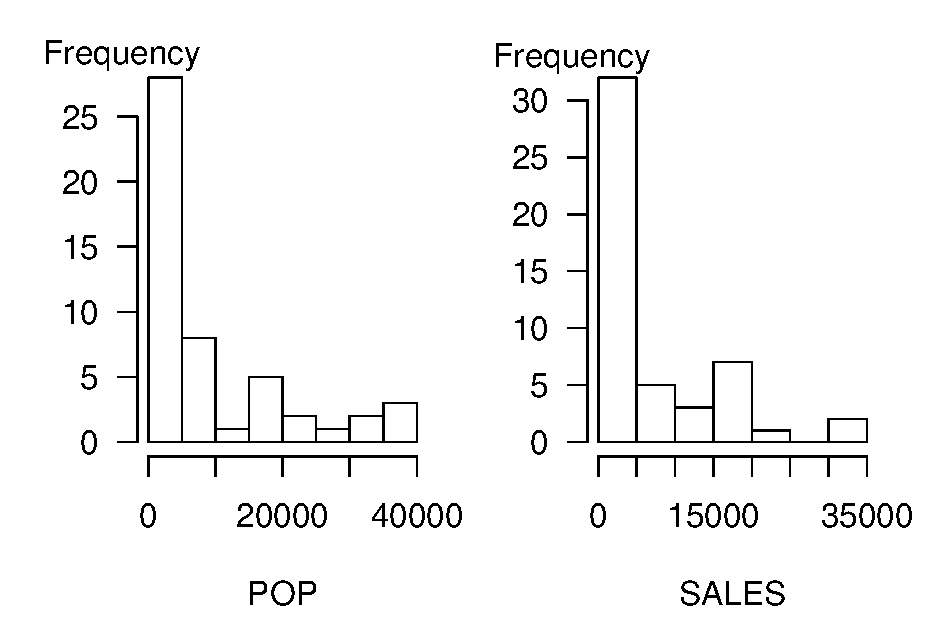
\includegraphics[width=0.6\textwidth]
    {Chapter2/F2HistPopSales.eps}
    \caption{\label{F2:HistPopSales} \small Histograms of Population and Sales.
    Each distribution is skewed to the right, indicating that there are many
    small areas compared to a few areas with larger sales and populations.}
  \end{center}
\end{figure}

\begin{table}[h] \scalefont{0.9}
\caption{\label{T2:SummaryStats}
Summary Statistics of Each Variable}
\begin{tabular}{lrrrrr}
\hline
&  &  & Standard &  &  \\
Variable & Mean & Median & Deviation & Minimum & Maximum \\ \hline
POP & 9,311 & 4,406 & 11,098 & 280 & 39,098 \\
SALES & 6,495 & 2,426 & 8,103 & 189 & 33,181 \\ \hline
\end{tabular}


\textit{Source: Frees and Miller (2003).}
 \scalefont{1.1111}
\end{table}

\bigskip

As Table \ref{T2:SummaryStats} shows, the basic summary statistics
give useful ideas of the structure of key features of the data.
After we understand the information in each variable in isolation of
the other, we can begin exploring the relationship between the two
variables.

\linetjed

\subsubsection*{Scatter Plot and Correlation Coefficients - Basic Summary
Tools}\index{plots!scatter}

The basic graphical tool used to investigate the relationship
between the two variables is a \emph{scatter plot} such as in Figure
\ref{F2:SalesVsPoP}. Although we may lose the exact values of the
observations when graphing data, we gain a visual impression of the
relationship between population and sales. From Figure
\ref{F2:SalesVsPoP} we see that areas with larger populations tend
to purchase more lottery tickets. How strong is this relationship?
Can knowledge of the area's population help us anticipate the
revenue from lottery sales? We explore these two questions below.

\begin{figure}[ht]
%\flushleft
    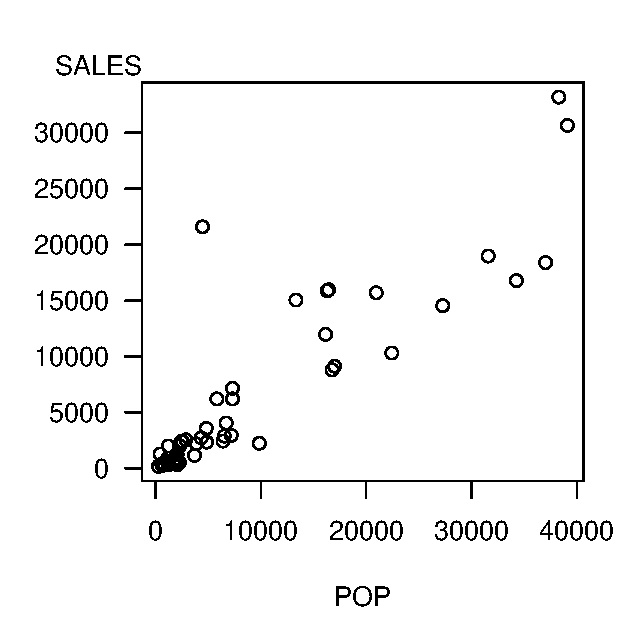
\includegraphics[width=0.6\textwidth]{Chapter2/F2SalesVsPoP.eps}
    \caption{\label{F2:SalesVsPoP} \small A scatter plot of the lottery data. Each of the 50
     plotting symbols corresponds to a zip code in the study. This figure suggests
     that postal areas with larger populations have larger lottery revenues.}
\end{figure}


One way to summarize the strength of the relationship between two
variables is through a \emph{correlation} statistic.

\bigskip

\boxedjed

\index{correlation coefficients!Pearson}\index{correlation
coefficients!ordinary}\index{symbols!$s_x$, sample standard
deviation of \{$x_1, \ldots, x_n$\}}\index{symbols!$s_y$, sample
standard deviation}

\textit{Definition}. The \emph{ordinary, or Pearson, correlation}
coefficient is defined as
\begin{equation*}
r=\frac{1}{(n-1)s_xs_y}\sum_{i=1}^{n}\left(
x_{i}-\overline{x}\right) \left( y_{i}-\overline{y}\right) .
\end{equation*}

\bigskip

\noindent Here, we use the sample standard deviation $s_y =
\sqrt{(n-1)^{-1} \sum_{i=1}^{n}\left( y_i -
\overline{y}\right)^{2}}$ defined in Section 1.2, with similar
notation for $s_x$.

\end{boxedminipage}

\bigskip

Although there are other correlation statistics, the correlation
coefficient devised by Pearson (1895) has several desirable
properties. One important property is that, for any data set, $r$ is
bounded by -1 and 1, that is, $-1\leq r\leq 1$. (Exercise 2A.9
provides steps for you to check this property.) If $r$ is greater
than zero, the variables are said to be \emph{(positively)
correlated}. If $r$ is less than zero, the variables are said to be
\emph{negatively correlated}. The larger the coefficient is in
absolute value, the stronger is the relationship. In fact, if $r=1$,
then the variables are perfectly correlated. In this case, all of
the data lie on a straight line that goes through the lower left and
upper right-hand quadrants. If $r=-1$, then all of the data lie on a
line that goes through the upper left and lower right-hand
quadrants. The coefficient $r$ is a measure of a \emph{linear}
relationship between two variables.

\marginparjed{The coefficient $r$ is a measure of a linear
relationship between two variables.}

The correlation coefficient is said to be \emph{location and scale
invariant}. Thus, each variable's center of location does not matter
in the calculation of $r$. For example, if we add \$100 to the sales
of each zip code, each $y_i$ will increase by 100. However,
$\overline{y}$, the average purchase price will also increase by 100
so that the deviation $y_i - \overline{y}$ remains unchanged, or
invariant. Further, the scale of each variable does not matter in
the calculation of $r$. For example, suppose we divide each
population by 1000 so that $x_i$ now represents population in
thousands. Thus, $\overline{x}$\ is also divided by 1000 and you
should check that $s_x$ is also divided by 1000. Thus, the
standardized version of $x_i$, $\left( x_i-\overline{x}\right)
/s_x$, remains unchanged, or invariant. Many statistical packages
compute a standardized version of a variable by subtracting the
average and dividing by the standard deviation. Now, let's use
$y_{i,std}=\left( y_i- \overline{y}\right) /s_y$ and
$x_{i,std}=\left( x_i-\overline{x} \right) /s_x$ to be the
standardized versions of $y_i$ and $x_i$, respectively. With this
notation, we can express the correlation coefficient as
$r=(n-1)^{-1}\sum_{i=1}^{n}x_{i,std}\times y_{i,std}.$

The correlation coefficient is said to be a \emph{dimensionless
measure}. This is because we have taken away dollars, and all other
units of measures, by considering the standardized variables
$x_{i,std}$ and $y_{i,std}$. Because the correlation coefficient
does not depend on units of measure, it is a statistic that can
readily be compared across different data sets.

\marginparjed{The correlation coefficient is location and scale
invariant. It is dimensionless.}

\index{explanatory variable!quadratic}

In the world of business, the term ``correlation'' is often used as
synonymous with the term ``relationship.'' For the purposes of this
text, we use the term correlation when referring only to linear
relationships. The classic nonlinear relationship is $y=x^{2}$, a
quadratic relationship. Consider this relationship and the
fictitious data set for $x$, $\{-2,1,0,1,2\}$. Now, as an exercise
(2.\ref{Ex:ZeroCorr}), produce a rough graph of the data set:

\scalefont{0.9}
\begin{center}
$
\begin{tabular}{l|rrrrr}
\hline
$i$ & 1 & 2 & 3 & 4 & 5 \\
$x_i$ & -2 & -1 & 0 & 1 & 2 \\
$y_i$ & 4 & 1 & 0 & 1 & 4 \\ \hline
\end{tabular}
$
\end{center}
\scalefont{1.1111}

\noindent The correlation coefficient for this data set turns out to be $r=0$
(check this). Thus, despite the fact that there is a perfect relationship
between $x$ and $y$ ($=x^{2}$), there is a zero correlation. Recall that
location and scale changes are not relevant in correlation discussions, so
we could easily change the values of $x$ and $y$ to be more representative
of a business data set.

How strong is the relationship between $y$ and $x$ for the lottery
data? Graphically, the response is a scatter plot, as in Figure
\ref{F2:SalesVsPoP}. Numerically, the main response is the
correlation coefficient which turns out to be $r$ = 0.886 for this
data set. We interpret this statistic by saying that SALES and POP
are (positively) correlated. The strength of the relationship is
strong because $r$ = 0.886 is close to one. In summary, we may
describe this relationship by saying that there is a strong
correlation between SALES and POP.

\subsubsection*{Method of Least Squares}\index{least squares!method}

Now we begin to explore the question, ``Can knowledge of population
help us understand sales?'' To respond to this question, we identify
sales as the \emph{response}, or \emph{dependent, variable}. The
population variable, which is used to help understand sales, is
called the \emph{explanatory}, or \emph{independent, variable}.

Suppose that we have available the sample data of fifty sales $\{y_1, \ldots, y_{50} \}$ and your job
is to predict the sales of a randomly selected ZIP code. Without
knowledge of the population variable, a sensible predictor is simply
$\overline{y}=6,495$, the average of the available sample.
Naturally, you anticipate that areas with larger populations will
have larger sales. That is, if you also have knowledge of
population, then can this estimate be improved? If so, then by how
much?

To answer these questions, the first step assumes an approximate
linear relationship between $x$ and $y$. To fit a line to our data
set, we use the \emph{method of least squares}. We need a general
technique so that, if different analysts agree on the data and agree
on the fitting technique, then they will agree on the line. If
different analysts fit a data set using eyeball approximations, in
general they will arrive at different lines, even using the same
data set.

The method\ begins with the line $y=b_0^{\ast}+b_1^{\ast}x$, where
the intercept and slope, $b_0^{\ast}$ and $b_1^{\ast}$, are merely
generic values. For the $i$th observation, $y_i-\left(
b_0^{\ast}+b_1^{\ast}x_i\right) $ represents the deviation of the
observed value $y_i$ from the line at $x_i$. The quantity
\begin{equation*}
SS(b_0^{\ast},b_1^{\ast})=\sum_{i=1}^{n}\left( y_i-\left(
b_0^{\ast}+b_1^{\ast}x_i\right) \right) ^{2}
\end{equation*}
represents the sum of squared deviations for this candidate line.
The least squares method consists of determining the values of
$b_0^{\ast}$ and $b_1^{\ast}$\ that minimize
$SS(b_0^{\ast},b_1^{\ast})$. This is an easy problem that can be
solved by calculus, as follows. Taking partial derivatives with
respect to each argument yields
\begin{equation*}
\frac{\partial }{\partial
b_0^{\ast}}SS(b_0^{\ast},b_1^{\ast})=\sum_{i=1}^{n}(-2)\left(
y_i-\left( b_0^{\ast}+b_1^{\ast}x_i\right) \right)
\end{equation*}
and
\begin{equation*}
\frac{\partial }{\partial
b_1^{\ast}}SS(b_0^{\ast},b_1^{\ast})=\sum_{i=1}^{n}(-2x_i)\left(
y_i-\left( b_0^{\ast}+b_1^{\ast}x_i\right) \right) .
\end{equation*}
The reader is invited to take second partial derivatives to ensure
that we are minimizing, not maximizing, this function. Setting these
quantities equal to zero \ and canceling constant terms yields
\begin{equation*}
\sum_{i=1}^{n}\left( y_i-\left( b_0^{\ast}+b_1^{\ast}x_i\right)
\right) =0
\end{equation*}
and
\begin{equation*}
\sum_{i=1}^{n}x_i\left( y_i-\left( b_0^{\ast}+b_1^{\ast}x_i\right)
\right) =0,
\end{equation*}
which are known as the \emph{normal equations}. Solving these
equations yields the values of $b_0^{\ast}$ and $b_1^{\ast}$ that
minimize the sum of squares, as follows.\index{normal equations}

\bigskip

\boxedjed \index{least squares!intercept}\index{least
squares!slope}\index{symbols!$b_0$, least squares
intercept}\index{symbols!$b_1$, least squares
slope}\index{symbols!$\widehat{y}$, fitted value of $y$}

\textit{Definition. }The \emph{least squares intercept and slope
estimates} are

\begin{equation*}
b_1=r\frac{s_y}{s_x}~~~~~\mathrm{and}~~~~~b_0=\overline{y}-b_1
\overline{x}.
\end{equation*}
The line that they determine, $\widehat{y}=b_0+b_1x$, is called the
\emph{fitted regression line}.

\end{boxedminipage}
\bigskip

\noindent We have dropped the asterisk, or star, notation because
$b_0$ and $b_1$ are no longer ``candidate'' values.

Does this procedure yield a sensible line for our Wisconsin lottery
sales? Earlier, we computed $r=0.886$. From this and the basic
summary statistics in Table \ref{T2:SummaryStats}, we have $b_1 =
0.886 \left( 8,103\right) /11,098=0.647$ and $b_0 =
6,495-(0.647)9,311 = 469.7.$ This yields the fitted regression line
\begin{equation*}
\widehat{y} = 469.7 + (0.647)x.
\end{equation*}
The carat, or ``hat,'' on top of the $y$ reminds us that this
$\widehat{y}$, or $\widehat{SALES}$, is a fitted value. One
application of the regression line is to estimate sales for a
specific population say, $x=10,000$. The estimate is the height of
the regression line, which is $469.7 + (0.647)(10,000) = 6,939.7$.

\linejed

\index{examples!summarizing simulations}\index{actuarial \&
financial terms and concepts!value-at-risk, VaR}\index{actuarial \&
financial terms and concepts!conditional tail expectation, CTE}

\textbf{Example: Summarizing Simulations.}\ecaptionjed{Summarizing
Simulations} Regression analysis is a tool for summarizing complex
data. In practical work, actuaries often simulate complicated
financial scenarios; it is often overlooked that regression can be
used to summarize relationships of interest.

To illustrate, Manistre and Hancock (2005) simulated many
realizations of a 10-year European put option and demonstrated the
relationship between two actuarial risk measures, the value-at-risk
(VaR) and the conditional tail expectation (CTE). For one example,
these authors examined lognormally distributed stock returns with an
initial stock price of \$100, so that in 10 years the price of the
stock would be distributed as
\begin{equation*}
S(Z)=100 \exp \left( (.08) 10 + .15 \sqrt{10} Z \right),
\end{equation*}
based on an annual mean return of 10\%, standard deviation 15\% and
the outcome from a standard normal random variable $Z$. The put
option pays the difference between the strike price, that will be
taken to be 110 for this example, and $S(Z)$. The present value of
this option is
\begin{equation*}
C(Z)= \mathrm{e}^{-0.06(10)} \mathrm{max} \left(0, 110-S(Z) \right),
\end{equation*}
based on a 6\% discount rate.

To estimate the VaR and CTE, for each $i$, 1000 i.i.d. standard
normal random variables were simulated and used to calculate 1000
present values, $C_{i1}, \ldots, C_{i,1000}.$ The 95th percentile of
these present values is the estimate of the value at risk, denoted
as $VaR_i.$ The average of the highest 50 ($= (1-.05) \times 1000$)
of the present values is the estimate of the conditional tail
expectation, denoted as $CTE_i$. Manistre and Hancock (2005)
performed this calculation $i=1, \ldots, 1000$ times; the result is
presented in Figure \ref{F2:VarCTE}. The scatterplot shows a strong
but not perfect relationship between the $VaR$ and the $CTE$, the
correlation coefficient turns out to be $r=0.782$.


\begin{figure}[htp]
  \begin{center}
   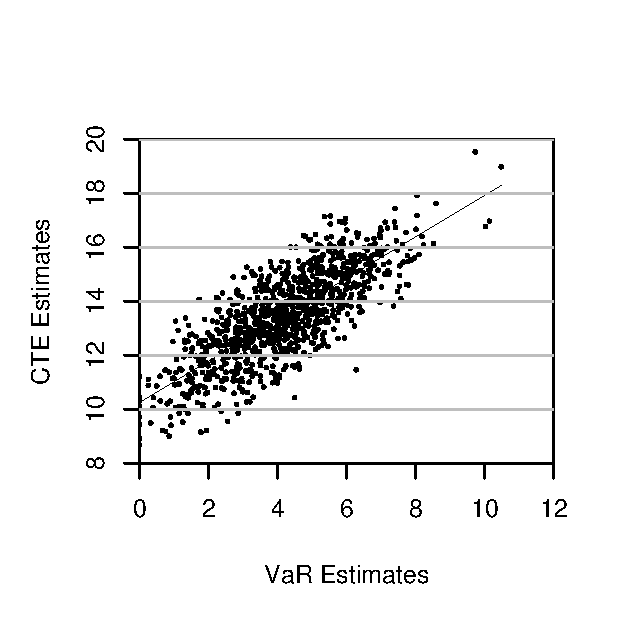
\includegraphics[width=0.6\textwidth]{Chapter2/VarCTEFig.eps}
    \caption{\label{F2:VarCTE} \small Plot of Conditional Tail Expectation (CTE) versus Value at Risk (VaR).
    Based on $n=1,000$ simulations from a 10-year European put bond. \textit{Source: Manistre and
Hancock (2005)}}
  \end{center}
\end{figure}

\linejed


\section{Basic Linear Regression Model}\index{regression model!basic linear}\index{regression model!simple linear}

The scatter plot, correlation coefficient and the fitted regression
line are useful devices for summarizing the relationship between two
variables for a specific data set. To infer general relationships,
we need models to represent outcomes of broad populations.

This chapter focuses on a ``basic linear regression'' model. The
``linear regression'' part comes from the fact that we fit a line to
the data. The ``basic'' part is because we use only one explanatory
variable, $x$. This model is also known as a ``simple'' linear
regression. This text avoids this language because it gives the
false impression that regression ideas and interpretations with one
explanatory variable are always straightforward.

We now introduce two sets of assumptions of the basic model, the
``observables'' and the ``error'' representations. They are
equivalent but each will help us as we later extend regression
models beyond the basics.\index{model assumptions!observables
representation}\index{symbols!$\beta_0$, (population) regression
intercept}\index{symbols!$\beta_1$, (population) regression
coefficient associated with $x_1$}

\begin{center}\scalefont{0.9}
\begin{tabular}{c}
\hline
Basic Linear Regression Model \\
Observables Representation Sampling Assumptions \\ \hline
\multicolumn{1}{l}{F1. $\mathrm{E}~y_i=\beta_0 + \beta_1 x_i $.} \\
\multicolumn{1}{l}{F2. $\{x_1,\ldots ,x_n\}$ are non-stochastic
variables.} \\
\multicolumn{1}{l}{F3. $\mathrm{Var}~y_i=\sigma ^{2}$.} \\
\multicolumn{1}{l}{F4. \{$y_i$\} are independent random variables.} \\
\hline
\end{tabular}\scalefont{1.1111}
\end{center}

The ``observables representation'' focuses on variables that we can
see (or observe), $(x_i,y_i)$. Inference about the distribution of
$y$ is conditional on the observed explanatory variables, so that we
may treat $\{x_1,\ldots ,x_n\}$ as non-stochastic variables
(assumption F2). When considering types of sampling mechanisms for
$(x_i,y_i)$, it is convenient to think of a \emph{stratified random
sampling} scheme, where values of $\{x_1,\ldots ,x_n\}$ are treated
as the strata, or group. Under stratified sampling, for each unique
value of $x_i$, we draw a random sample from a population. To
illustrate, suppose you are drawing from a database of firms to
understand stock return performance ($y$) and wish to stratify based
on the size of the firm. If the amount of assets is a
continuous variable, then we can imagine drawing a sample of size 1
for each firm. In this way, we hypothesize a distribution of stock
returns conditional on firm asset size.

\emph{Digression}: You will often see reports that summarize results for the ``top 50
managers'' or the ``best 100 universities,'' measured by some
outcome variable. In regression applications, make sure that you do
not select observations based on a dependent variable, such as
the highest stock return, because this is stratifying
based on the $y$, not the $x$. Chapter 6 will discuss sampling procedures in greater detail.

Stratified sampling also provides motivation for assumption F4, the
independence among responses. One can motivate assumption F1 by
thinking of $(x_i,y_i)$ as a draw from a population, where the mean
of the conditional distribution of $y_i$ given \{$x_i$\} is linear
in the explanatory variable. Assumption F3 is known as
\emph{homoscedasticity} that we will discuss extensively in Section
5.7. See Goldberger (1991) for additional background on this
representation.\index{homoscedasticity}

A fifth assumption that is often implicitly used is:

\begin{center}
F5. \{$y_i$\} are normally distributed.
\end{center}

\noindent This assumption is not required for many statistical inference
procedures because central limit theorems provide approximate normality for
many statistics of interest. However, formal justification for some, such as
$t$-statistics, do require this additional assumption.

In contrast to the observables representation, an alternative set of
assumptions focuses on the deviations, or ``errors,'' in the
regression, defined as $\varepsilon_i=y_i-\left( \beta_0 + \beta_1
x_i \right) $.\index{model assumptions!error
representation}\index{symbols!$\varepsilon_i$, ``error,'' or
disturbance term}

\begin{center}\scalefont{0.9}
\begin{tabular}{c}
\hline
Basic Linear Regression Model \\
Error Representation Sampling Assumptions \\ \hline
\multicolumn{1}{l}{E1. $y_i=\beta_0+\beta_1 x_i + \varepsilon _i$.}
\\
\multicolumn{1}{l}{E2. $\{x_1,\ldots ,x_n\}$ are non-stochastic
variables.} \\
\multicolumn{1}{l}{E3. $\mathrm{E}~\varepsilon _i=0$ and $\mathrm{Var}~\varepsilon _i=\sigma ^{2}$.} \\
\multicolumn{1}{l}{E4. \{$\varepsilon _i$\} are independent random
variables.} \\ \hline
\end{tabular}\scalefont{1.1111}
\end{center}

The ``error representation'' is based on the Gaussian theory of
errors (see Stigler, 1986, for a historical background). Assumption
E1 assumes that $y$ is in part due to a linear function of the
observed explanatory variable, $x$. Other unobserved variables that
influence the measurement of $y$ are interpreted to be included in
the ``error'' term $\varepsilon _i$, which is also known as the
``disturbance'' term. The independence of errors, E4, can be
motivated by assuming that \{$\varepsilon _i$\} are realized through
a simple random sample from an unknown population of errors.

Assumptions E1-E4 are equivalent to F1-F4. The error representation
provides a useful springboard for motivating goodness of fit
measures (Section \ref{S2:SummStats}). However, a drawback of the
error representation is that it draws the attention from the
observable quantities $(x_i,y_i)$ to an unobservable quantity,
\{$\varepsilon _i$\}. To illustrate, the sampling basis, viewing
\{$\varepsilon _i$\} as a simple random sample, is not directly
verifiable because one cannot directly observe the sample \{$
\varepsilon _i$\}. Moreover, the assumption of additive errors in E1
will be troublesome when we consider nonlinear regression models.

Figure \ref{F2:NormalCurve} illustrates some of the assumptions of
the basic linear regression model. The data ($x_1,y_1$), ($x_2,y_2$)
and ($x_3,y_3$) are observed and are represented by the circular
opaque plotting symbols. According to the model, these observations
should be close to the regression line $\mathrm{E}~y = \beta_0 +
\beta_1 x$. Each deviation from the line is random. We will often
assume that the distribution of deviations may be represented by a
normal curve, as in Figure \ref{F2:NormalCurve}.


\begin{figure}[htp]
  \begin{center}
    %  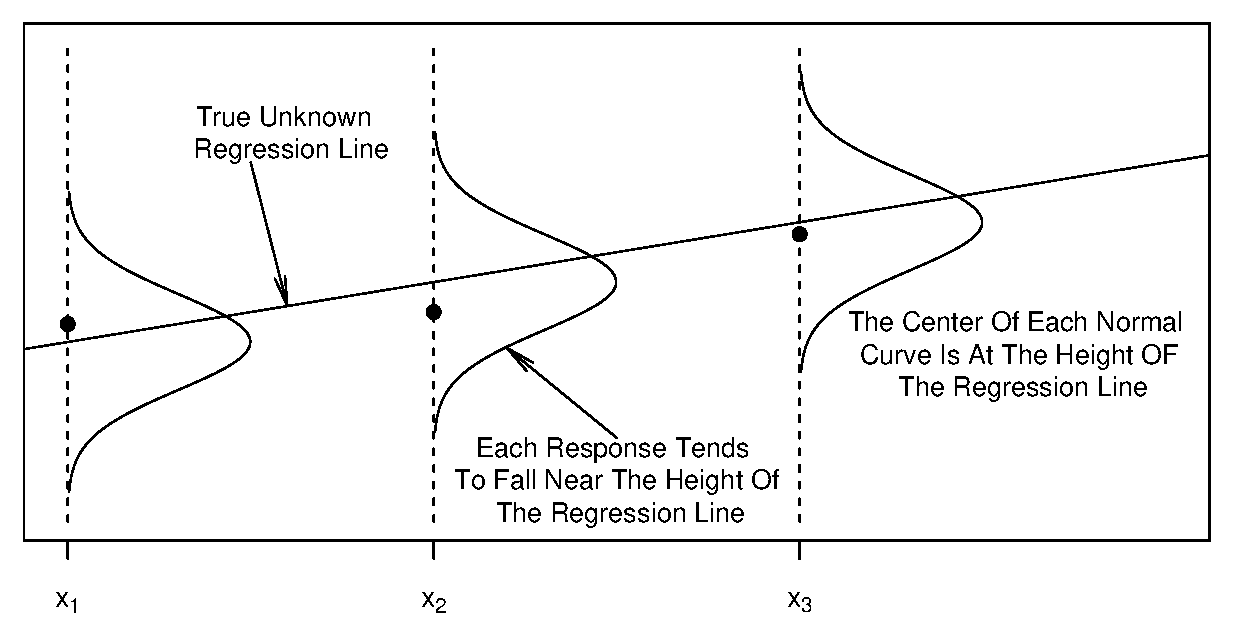
\includegraphics[width=1\textwidth,angle=270,scale=.75]{Chapter2/F2NormalCurve.ps}
    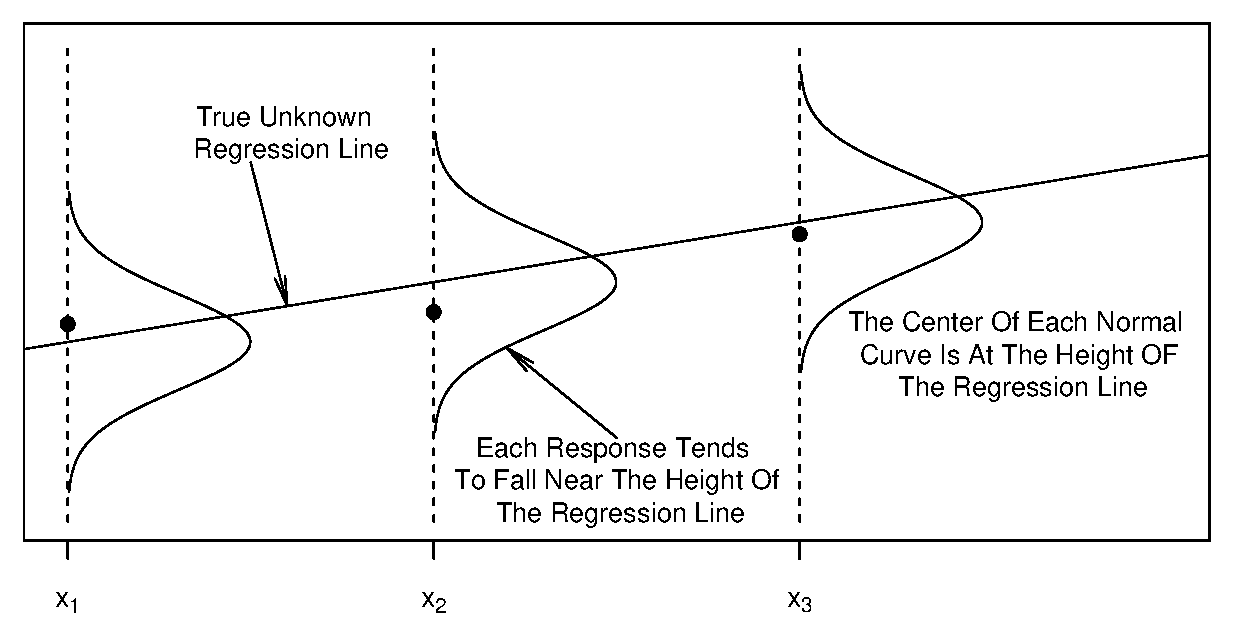
\includegraphics[width=0.8\textwidth]{Chapter2/F2NormalCurve.eps}
    \caption{\label{F2:NormalCurve} \small The distribution of the response varies by the level of the
explanatory variable.}
  \end{center}
\end{figure}

The basic linear regression model assumptions describe the
underlying population. Table \ref{T2:SumPopSample} highlights the
idea that characteristics of this population can be summarized by
the parameters $\beta_0$, $\beta_1$ and $\sigma ^{2}$. In Section
2.1, we summarized data from a sample, introducing the statistics
$b_0$ and $b_1$. Section \ref{S2:SummStats} will introduce $s^{2}$,
the statistic corresponding to the parameter $\sigma ^{2}$.

\begin{table}[h]
\caption{\label{T2:SumPopSample} Summary Measures of the Population
and Sample}
\begin{tabular}{ccccc}
\hline
Data & Summary & \multicolumn{2}{c}{Regression} & Variance \\
& Measures & \multicolumn{2}{c}{Line} &  \\ \cline{3-4}
\vspace{-0.1in} \\& & Intercept & Slope &  \\ \hline
Population & Parameters & $\beta_0$ & $\beta_1$ & $\sigma ^{2}$ \\
Sample & Statistics & $b_0$ & $b_1$ & $s^2$ \\ \hline
\end{tabular}
\end{table}

\section{Is the Model Useful? Some Basic Summary
Measures}\label{S2:SummStats}

Although statistics is the science of summarizing data, it is also
the art of arguing with data. This section develops some of the
basic tools used to justify the basic linear regression model. A
scatter plot may provide strong \emph{visual} evidence that $x$
influences $y$; developing \emph{numerical} evidence will enable us
to quantify the strength of the relationship. Further, numerical
evidence will be useful when we consider other data sets where the
graphical evidence is not compelling.

\subsection{Partitioning the Variability}

The squared deviations, $\left( y_i-\overline{y}\right) ^2$, provide
a basis for measuring the spread of the data. If we wish to estimate
the $i$th dependent variable \emph{without} knowledge of $x$, then
$\overline{y}$\ is an appropriate estimate and $y_i- \overline{y}$
represents the deviation of the estimate. We use
$Total~SS=\sum_{i=1}^{n}\left( y_i-\overline{y}\right) ^2$, the
total sum of squares, to represent the variation in all of the
responses.\index{symbols!$Total~SS$, total sum of squares}

Suppose now that we also have knowledge of $x$, an explanatory
variable. Using the fitted regression line, for each observation we
can compute the corresponding\emph{\ fitted value}, $\widehat{y}_i =
b_0 + b_1x_i$. The fitted value is our estimate \emph{with}
knowledge of the explanatory variable. As before, the difference
between the response and the fitted value, $y_i- \widehat{y}_i$,
represents the deviation of this estimate. We now have two
``estimates'' of $y_i$, these are $\widehat{y}_i$ and
$\overline{y}$. Presumably, if the regression line is useful, then $
\widehat{y}_i$ is a more accurate measure than $\overline{y}$. To
judge this usefulness, we algebraically decompose the total
deviation as:
\begin{equation}\label{E2:deviationdecomp}
\begin{tabular}{ccccc}
$\underbrace{y_i-\overline{y}}$ & = &
$\underbrace{y_i-\widehat{y}_i}$
& + & $\underbrace{\widehat{y}_i-\overline{y}}$ \\
{\small total} & {\small =} & {\small unexplained} & {\small +} &
{\small
explained} \\
{\small deviation} &  & {\small deviation} &  & {\small deviation}
\end{tabular}
\end{equation}
Interpret this equation as ``the deviation without knowledge of $x$
equals the deviation with knowledge of $x$ plus the deviation
explained by $x$.'' Figure \ref{F2:ANOVADecomp} is a geometric
display of this decomposition. In the figure, an observation above
the line was chosen, yielding a positive deviation from the fitted
regression line, to make the graph easier to read. A good exercise
is to draw a rough sketch corresponding to Figure
\ref{F2:ANOVADecomp} with an observation below the fitted regression
line.

\begin{figure}[htp]
  \begin{center}
    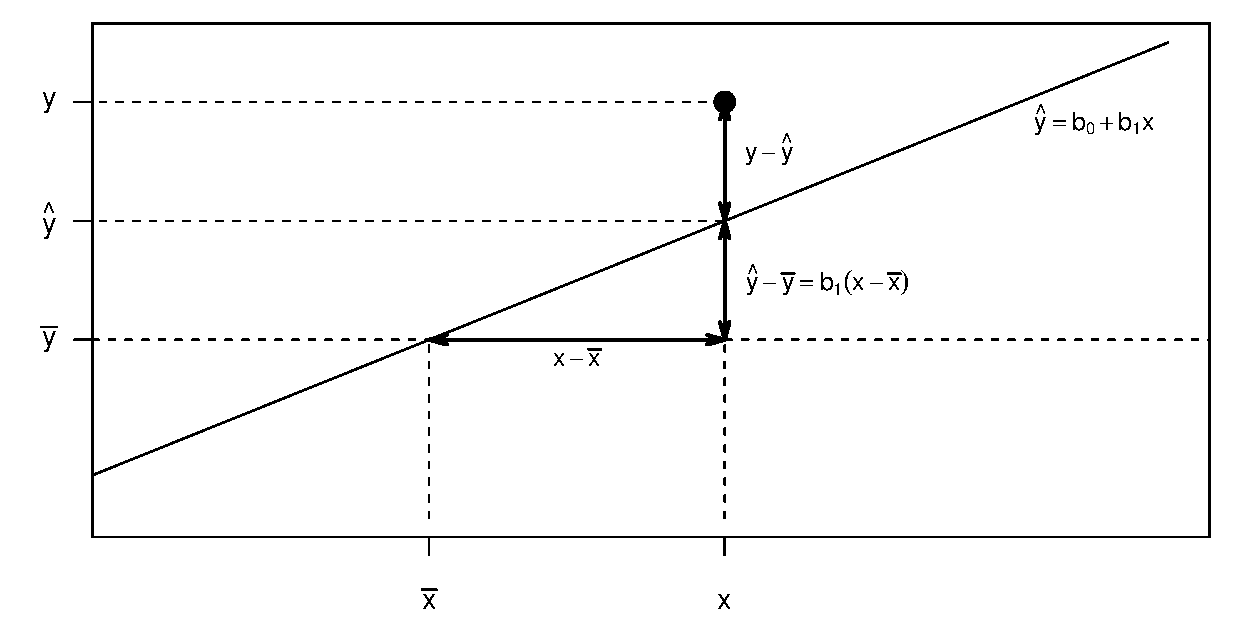
\includegraphics[width=0.8\textwidth]{Chapter2/F2ANOVADecomp.eps}
    \caption{\label{F2:ANOVADecomp} \small Geometric display of the deviation decomposition.}
  \end{center}
\end{figure}

\bigskip

Now, from the algebraic decomposition in equation
(\ref{E2:deviationdecomp}), square each side of the equation and sum
over all observations. After a little algebraic manipulation, this
yields
\begin{equation}\label{E2:ANOVADecomposition}
\sum_{i=1}^{n}\left( y_i-\overline{y}\right) ^2=\sum_{i=1}^{n}\left(
y_i-\widehat{y}_i\right) ^2+\sum_{i=1}^{n}\left( \widehat{y}_i-
\overline{y}\right) ^2.
\end{equation}
We rewrite this as $Total~SS=Error~SS+Regression~SS$ where $SS$ stands for
sum of squares. We interpret:

\begin{itemize}
\item $Total~SS$ as the total variation without knowledge of $x$,

\item $Error~SS$ as the total variation remaining after the introduction of $x$, and

\item $Regression~SS$ as the difference between the $Total~SS$ and $Error~SS$
, or the total variation ``explained'' through knowledge of $x$.
\end{itemize}

\index{symbols!$Error~SS$, error sum of
squares}\index{symbols!$Regression~SS$, regression sum of squares}



\noindent When squaring the right-hand side of equation
(\ref{E2:deviationdecomp}), we have the cross-product term $2\left(
y_i-\widehat{y}_i\right) \left( \widehat{y}_i-\overline{y}\right) $.
With the ``algebraic manipulation,'' one can check that the sum of
the cross-products over all observations is zero. This result is not
true for all fitted lines but is a special property of the least
squares fitted line.

In many instances, the variability decomposition is reported through only a
single statistic.

\bigskip\index{goodness of fit statistics!coefficient of
determination, $R^2$}\index{symbols!$R^2$, coefficient of
determination}

\boxedjed

\textit{Definition.} The \emph{coefficient of determination} is
denoted by the symbol $R^2$, called ``$R$-square,'' and defined as
\begin{equation*}
R^2=\frac{Regression~SS}{Total~SS}.
\end{equation*}

\end{boxedminipage}
\bigskip

\noindent We interpret $R^2$ to be the proportion of variability
explained by the regression line. In one extreme case where the
regression line fits the data perfectly, we have $Error~SS=0$ and
$R^2=1$. In the other extreme case where the regression line
provides no information about the response, we have
$Regression~SS=0$ and $R^2=0.$ The coefficient of determination is
constrained by the inequalities $0 \leq R^2 \leq 1$ with larger
values implying a better fit.

\subsection{The Size of a Typical Deviation: \textit{s}}

In the basic linear regression model, the deviation of the response
from the regression line, $y_i-\left( \beta_0+\beta_1x_i\right) $,
is not an observable quantity because the parameters $\beta_0$ and
$\beta_1$ \ are not observed. However, by using estimators $b_0$ and
$b_1$, we can approximate this deviation using
\begin{equation*}
e_i=y_i-\widehat{y}_i=y_i-\left( b_0+b_1x_i\right) ,
\end{equation*}
known as the \emph{residual}.\index{residual}\index{symbols!$e_i$,
residual}

Residuals will be critical to developing strategies for improving
model specification in Section \ref{S2:ResidualAnalsis}. We now show
how to use the residuals to estimate $\sigma ^2$. From a first
course in statistics, we know that if one could observe the
deviations $\varepsilon _i$, then a desirable estimate of $\sigma
^2$\ would be $(n-1)^{-1}\sum_{i=1}^{n}\left( \varepsilon
_i-\overline{\varepsilon }\right) ^2$. Because \{$\varepsilon _i$\}
are not observed, we use the following.

\bigskip\index{symbols!$s^2$, mean square error}
\index{symbols!$s$, residual standard deviation}

\boxedjed

\textit{Definition}. An estimator of $\sigma ^2$, the \emph{mean
square error (MSE)}, is defined as
\begin{equation}
s^2=\frac{1}{n-2}\sum_{i=1}^{n}e_i{}^2.  \label{BLRs2}
\end{equation}
The positive square root, $s=\sqrt{s^2},$ is called the
\emph{residual standard deviation}.

\end{boxedminipage}
\bigskip

Comparing the definitions of $s^2$ and
$(n-1)^{-1}\sum_{i=1}^{n}\left( \varepsilon _i-\overline{\varepsilon
}\right) ^2$, you will see two important differences. First, in
defining $s^2$ we have not subtracted the average residual from each
residual before squaring. This is because the average residual is
zero, a special property of least squares estimation (see Exercise
2.\ref{Ex:AverageResid}). This result can be shown using algebra and
is guaranteed for all data sets.

\marginparjed{$s^2$ is an unbiased estimator of $\sigma ^2$.}

Second, in defining $s^2$ we have divided by $n-2$ instead of $n-1$.
Intuitively, dividing by either $n$ or $n-1$ tends to underestimate
$\sigma ^2$. The reason is that, when fitting lines to data, we need
at least two observations to determine a line. For example, we must
have at least three observations for there to be any variability
about a line. How much ``freedom'' is there for variability about a
line? We will say that the error degrees of freedom is the number of
observations available, $n$, minus the number of observations needed
to determine a line, 2 (with symbols, $df=n-2$). However, as we saw
in the least squares estimation subsection, we do not need to identify
two actual observations to determine a line. The idea is that if an
analyst knows the line and $n-2$ observations, then the remaining
two observations can be determined, without variability. When
dividing by $n-2$, it can be shown that $s^2$ is an unbiased
estimator of $\sigma ^2$.

We can also express $s^2$ in terms of the sum of squares quantities.
That is,

\begin{equation*}
s^2=\frac{1}{n-2}\sum_{i=1}^{n}\left( y_i-\widehat{y}_i\right) ^2=
\frac{Error~SS}{n-2}=MSE.
\end{equation*}

\index{analysis of variance, ANOVA, table}

This leads us to the \emph{analysis of variance}, or \emph{ANOVA},
table:

\scalefont{0.8}

\begin{center}
\begin{tabular}{llcl}
\hline
\multicolumn{4}{c}{ANOVA\ Table} \\ \hline
Source & Sum of Squares & $df$ & Mean Square \\ \hline
Regression & $Regression~SS$ & $1$ & $Regression~MS$ \\
Error & $Error~SS$ & $n-2$ & $MSE$ \\
Total & $Total~SS$ & $n-1$ &  \\ \hline
\end{tabular}
\end{center}

\scalefont{1.25}

\noindent The ANOVA table is merely a bookkeeping device used to
keep track of the sources of variability; it routinely appears in
statistical software packages as part of the regression output. The
mean square column figures are defined to be the sums of square
($SS$) figures divided by their respective degrees of freedom
($df$). In particular, the mean square for errors ($MSE$) equals $
s^2$ and the regression sum of squares equals the regression mean
square. This latter property is specific to the regression with one
variable case; it is not true where we consider more than one
explanatory variable.

The error degrees of freedom in the ANOVA table is $n-2$. The total degrees
of freedom is $n-1$, reflecting the fact that the total sum of squares is centered about the mean (at least two observations are required for positive variability). The single degree of freedom associated with the regression
portion means that the slope, plus one observation, is enough information to
determine the line. This is because it takes two observations to determine a
line and at least three observations for there to be any variability about
the line.

The analysis of variance table for the lottery data is:

\scalefont{0.8}

\begin{center}
\begin{tabular}{llll}
\hline
\multicolumn{4}{c}{ANOVA\ Table} \\ \hline
Source & Sum of Squares & $df$ & Mean Square \\ \hline
Regression & \multicolumn{1}{r}{2,527,165,015} & \multicolumn{1}{r}{1} &
\multicolumn{1}{r}{2,527,165,015} \\
Error & \multicolumn{1}{r}{690,116,755} & \multicolumn{1}{r}{48} &
\multicolumn{1}{r}{14,377,432} \\
Total & \multicolumn{1}{r}{3,217,281,770} & \multicolumn{1}{r}{49} &
\multicolumn{1}{r}{} \\ \hline
\end{tabular}
\end{center}
\scalefont{1.25}

 \noindent From this table, you can check that
$R^2=78.5\%$ and $s=3,792.$

\section{Properties of Regression Coefficient Estimators}

The least squares estimates can be expressed as weighted sum of the
responses. To see this, define the weights
\begin{equation*}
w_i=\frac{x_i-\overline{x}}{s_x^2(n-1)}.
\end{equation*}
Because the sum of $x$-deviations ($x_i-\overline{x}$) is zero, we
see that $\sum_{i=1}^{n}w_i=0$. Thus, we can express the slope
estimate
\begin{equation}
b_1=r\frac{s_y}{s_x}=\frac{1}{(n-1)s_x^2}\sum_{i=1}^{n}\left(
x_i-\overline{x}\right) \left( y_i-\overline{y}\right)
=\sum_{i=1}^{n}w_i\left( y_i-\overline{y}\right)
=\sum_{i=1}^{n}w_iy_i.  \label{weightb1}
\end{equation}

\noindent The exercises ask the reader to verify that $b_0$ can also
be expressed as a weighted sum of responses, so our discussion
pertains to both regression coefficients. Because regression
coefficients are weighted sums of responses, they can be affected
dramatically by unusual observations (see Section
\ref{S2:ResidualAnalsis}).

\marginparjed{Regression coefficients are weighted sums of the
responses.}

Because $b_1$ is a weighted sum, it is straightforward to derive the
expectation and variance of this statistic. By the linearity of
expectations and Assumption F1, we have
\begin{equation*}
\mathrm{E}~b_1=\sum_{i=1}^{n}w_i~\mathrm{E}~y_i=\beta_0\sum_{i=1}^{n}w_i+\beta_1\sum_{i=1}^{n}w_ix_i=\beta_1.
\end{equation*}
That is, $b_1$ is an unbiased estimator of $\beta_1$. Here, the sum
$ \sum_{i=1}^{n}w_ix_i$ $=$ \linebreak $\left[ s_x^2(n-1)\right]
^{-1}\sum_{i=1}^{n}\left( x_i-\overline{x}\right) x_i$ $=\left[
s_x^2(n-1)\right] ^{-1}\sum_{i=1}^{n}\left( x_i-\overline{x}\right)
^2=1.$ From the definition of the weights, some easy algebra also
shows that $\sum_{i=1}^{n}w_i^2=1/\left( s_x^2(n-1)\right) $.
Further, the independence of the responses implies that the variance
of the sum is the sum of the variances, and thus we have
\begin{equation*}
\mathrm{Var}~b_1=\sum_{i=1}^{n}w_i^2\mathrm{Var}~y_i=\frac{\sigma
^2}{s_x^2(n-1)}.
\end{equation*}
Replacing $\sigma ^2$\ by its estimator $s^2$ and taking square
roots leads to the following.

\bigskip\index{symbols!$se(b)$, standard error of $b$}

\boxedjed

\textit{Definition}. The \emph{standard error} of $b_1$, the
estimated standard deviation of $b_1$, is defined as
\begin{equation}
se(b_1)=\frac{s}{s_x\sqrt{n-1}}.  \label{seb1a}
\end{equation}

\end{boxedminipage}
\bigskip

This is our measure of the reliability, or precision, of the slope
estimator. Using equation (\ref{seb1a}), we see that $se(b_1)$ is
determined by three quantities, $n$, $s$ and $s_x$, as follows:

\marginparjed{A standard error is an estimated standard deviation.}


\begin{itemize}
\item If we have more observations so that $n$ becomes larger, then $
se(b_1)$ becomes smaller, other things equal.

\item If the observations have a greater tendency to lie closer to the line
so that $s$ becomes smaller, then $se(b_1)$ becomes smaller, other
things equal.

\item If values of the explanatory variable become more spread out so that $
s_x$ increases, then $se(b_1)$ becomes smaller, other things equal.
\end{itemize}

Smaller values of $se(b_1)$ offer a better opportunity to detect
relations between $y$ and $x$. Figure \ref{F2:BasicLSRE} illustrates
these relationships. Here, the scatter plot in the middle has the
smallest value of $se(b_1)$. Compared with the middle plot, the
left-hand plot has a larger value of $s$ and thus $se(b_1)$.
Compared with the right-hand plot, the middle plot has a larger
$s_x$, and thus smaller value of $se(b_1)$.

\noindent

\begin{figure}[htp]
  \begin{center}
    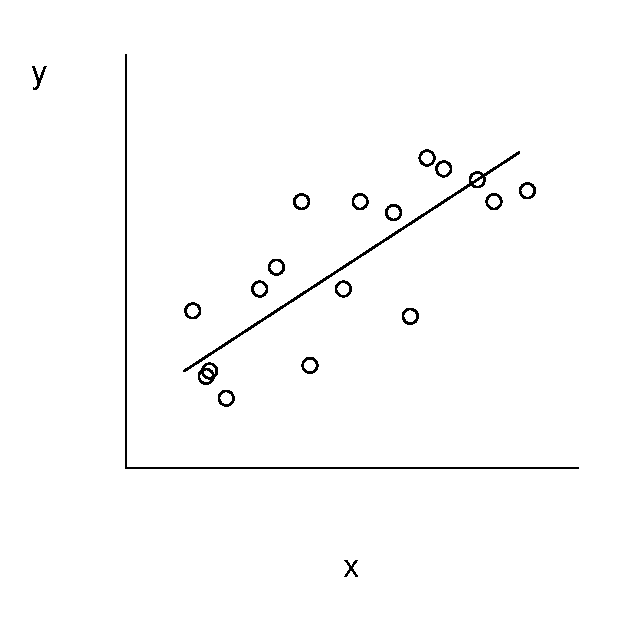
\includegraphics[height=1.8in,width=1.8in]{Chapter2/F2BasicLSRE1.eps}
    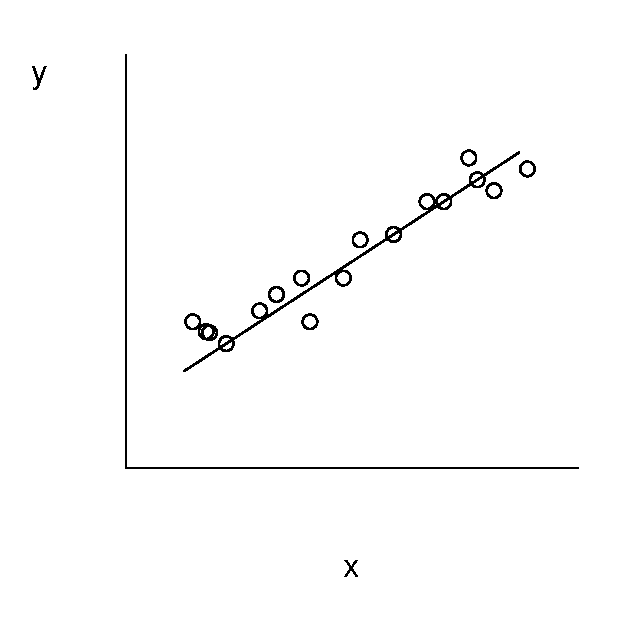
\includegraphics[height=1.8in,width=1.8in]{Chapter2/F2BasicLSRE2.eps} \hfill
    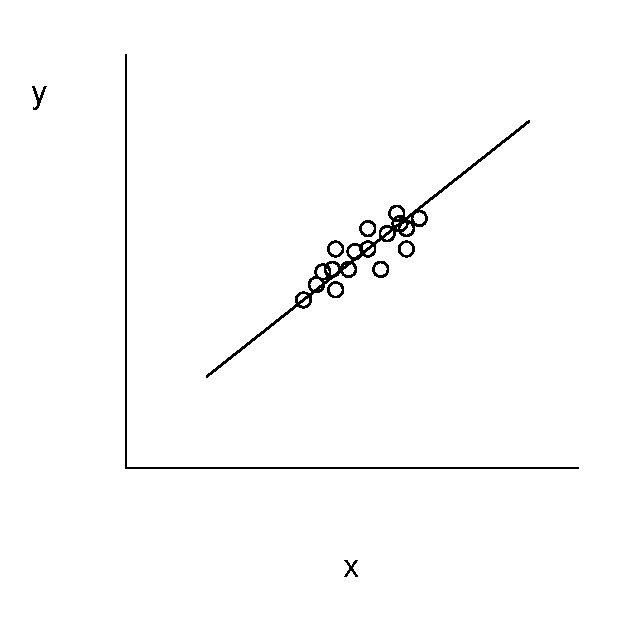
\includegraphics[height=1.8in,width=1.8in]{Chapter2/F2BasicLSRE3.eps} \hfill
    \caption{\label{F2:BasicLSRE} \small These three scatter plots exhibit the same linear
relationship between $y$ and $x$. The plot on the left exhibits
greater variability about the line than the plot in the middle. The
plot on the right exhibits a smaller standard deviation in $x$ than
the plot in the middle.}
  \end{center}
\end{figure}

\bigskip

Equation (\ref{weightb1}) also implies that the regression
coefficient $b_1 $ is normally distributed. That is, recall from
mathematical statistics that linear combinations of normal random
variables are also normal. Thus, if Assumption F5 holds, then $b_1$
is normally distributed. Moreover, several versions of central limit
theorems exists for weighted sums (see, for example, Serfling,
1980). Thus, as discussed in Section 1.4, if the responses $y_i$\
are even approximately normally distributed, then it will be
reasonable to use a normal approximation for the sampling
distribution of $b_1$. Using $se(b_1)$ as the estimated standard
deviation of $b_1$, for large values of $n$ we have that $\left(
b_1-\beta_1\right) /se(b_1)$ has an approximate standard normal
distribution. Although we will not prove it here, under Assumption
F5 $\left( b_1-\beta_1\right) /se(b_1)$\ follows a $t $-distribution
with degrees of freedom $df=n-2$.\index{theorems!central limit}

\section{Statistical Inference}

Having fit a model with a data set, we can make a number of important
statements. Generally, it is useful to think about these statements in three
categories: (i) tests of hypothesized ideas, (ii) estimates of model
parameters and (ii) predictions of new outcomes.

\subsection{Is the Explanatory Variable Important?: The
\textit{t}-Test}\index{hypothesis test!$t$-test}

We respond to the question of whether the explanatory variable is
important by investigating whether or not $\beta_1=0$. The logic is
that if $\beta_1=0$, then the basic linear regression model no
longer includes an explanatory variable $x$. Thus, we translate our
question of the importance of the explanatory variable into a
narrower question that can be answered using the hypothesis testing
framework. This narrower question is, is $ H_0:\beta_1=0$ valid? We
respond to this question by looking at the test statistic:

\begin{center}

\boxedjed
\begin{equation*}
t-\mathrm{ratio}=\frac{\mathrm{estimator-hypothesized~value~of~parameter}}
{\mathrm{standard~error~of~the~estimator}}.
\end{equation*}

\end{boxedminipage}
\end{center}

\index{symbols!$t(b)$, $t$-ratio for $b$}
\index{symbols!$t_{n-2,1-\alpha /2}$, a 1-$\alpha/2$ percentile from
the $t$-distribution with $n-2$ degrees of freedom}

\marginparjed{Appendix A3.3 provides additional details about the
$t$-distribution, including a graph and distribution table.}

For the case of $H_0:\beta_1=0$ , we examine $t$-ratio $
t(b_1)=b_1/se(b_1)$ because the hypothesized value of $\beta_1$\ is
0. This is the appropriate standardization because, under the null
hypothesis and the model assumptions described in Section 2.4, the
sampling distribution of $t(b_1)$ can be shown to be the
$t$-distribution with $ df=n-2$ degrees of freedom. Thus, to test
the null hypothesis $H_0$ against the alternative $H_{a}:\beta_1\neq
0$, we reject $H_0$ if favor of $H_{a}$ if $|t(b_1)|$ exceeds a
$t$-value. Here, this $t$-value is a percentile from the
$t$-distribution using $df=n-2$ degrees of freedom. \ We denote the
significance level as $\alpha $ \ and this $t$-value as
$t_{n-2,1-\alpha /2}$.\index{distributions!t-@{$t-$}}

\linejed

\textbf{Example: Lottery Sales - Continued.} For the lottery sales
example, the residual standard deviation is $s=3,792$. From Table
\ref{T2:SummaryStats}, we have $s_x = 11,098$. Thus, the standard
error of the slope is $se(b_1) = 3792/(11098\sqrt{50-1})=0.0488$.
From Section 2.1, the slope estimate is $b_1=0.647$. Thus, the
$t$-statistic is $t(b_1) = 0.647/0.0488 = 13.4$. We interpret this
by saying that the slope is 13.4 standard errors above zero. For the significance level,
we use the customary value of
$\alpha $ = 5\%. The 97.5th percentile from a $t$-distribution with
$df=50-2=48$ degrees of freedom is $t_{48,0.975}=2.011$. Because
$|13.4|>2.011$, we reject the null hypothesis that the slope
$\beta_1 = 0$ in favor of the alternative that $\beta_1 \neq 0$.

\linejed

\bigskip

\index{symbols!$H_0$, null hypothesis}\index{symbols!$H_a$,
alternative hypothesis}

Making decisions by comparing a $t$-ratio to a $t$-value is called a
$t$ \emph{-test}. Testing $H_0:\beta_1=0$ versus $H_{a}:\beta_1\neq
0$ is just one of many hypothesis tests that can be performed,
although it is the most common. Table \ref{T2:DecMakingProc}
outlines alternative decision-making procedures. These procedures
are for testing $H_0:\beta_1 = d$ where $d$ is a user-prescribed
value that may be equal to zero or any other known value. For
example, in our Section 2.7 example, we will use $d=1$ to test
financial theories about the stock market.


\begin{table}[h]
\caption{\label{T2:DecMakingProc} Decision-Making Procedures for
Testing $H_0:\beta_1 = d$}

\begin{tabular}{cc}
\hline Alternative Hypothesis ($H_{a}$) & Procedure: Reject $H_0$ in
favor of $ H_{a}$ if \\ \hline
$\beta_1>d$ & $t-\mathrm{ratio}>t_{n-2,1-\alpha }$. \\
$\beta_1<d$ & $t-\mathrm{ratio}<-t_{n-2,1-\alpha }$. \\
$\beta_1\neq d$ & $|t-\mathrm{ratio}\mathit{|}>t_{n-2,1-\alpha /2}$. \\
\hline \multicolumn{2}{l}{Notes: The significance level is
$\alpha $. Here, $t_{n-2,1-\alpha }$ is the (1-$\alpha $)th percentile}\\
\multicolumn{2}{l}{~~from the $t$-distribution using $df=n-2$
degrees
of freedom.} \\
\multicolumn{2}{l}{~~The test statistic is $t-\mathrm{ratio} = (b_1
-d)/se(b_1) $.} \\
 \hline
\end{tabular}

\end{table}

Alternatively, one can construct probability ($p$-) values and
compare these to given significant levels. The $p$-value is a useful
summary statistic for the data analyst to report since it allows the
report reader to understand the strength of the deviation from the
null hypothesis. Table \ref{T2:PvalueProc} summarizes the procedure
for calculating $p$-values.

\index{symbols!$p$-value, probability value}

\begin{table}[h]
\caption{\label{T2:PvalueProc} Probability Values for Testing
$H_0:\beta_1 = d$}
\begin{tabular}{cccc}
\hline
Alternative &  &  &  \\
Hypothesis ($H_a$) & $\beta_1>d$ & $\beta_1<d$ & $\beta_1\neq d$
\\ \hline
$p$-value & Pr($t_{n-2}>t-\mathrm{ratio}$) &
Pr($t_{n-2}<t-\mathrm{ratio}$) & $\mathrm{Pr}
(|t_{n-2}|>|t-\mathrm{ratio}\mathit{|})$ \\
\hline \multicolumn{4}{l}{Notes: Here, $t_{n-2}$
is a $t$-distributed random variable with $df=n-2$ degrees } \\
\multicolumn{4}{l}{~~of freedom. The test statistic is
$t-\mathrm{ratio} = (b_1 -d)/se(b_1) $.} \\
\hline
\end{tabular}
\end{table}

Another interesting way of addressing the question of the importance
of an explanatory variable is through the correlation coefficient.
Remember that the correlation coefficient is a measure of linear
relationship between $x$ and $y$. Let's denote this statistic by
$r(y,x)$. This quantity is unaffected by scale changes in either
variable. For example, if we multiply the $x$ variable by the number
$b_1$, then the correlation coefficient remains unchanged. Further,
correlations are unchanged by additive shifts. Thus, if we add a
number, say $b_0$, to each $x$ variable, then the correlation
coefficient remains unchanged. Using a scale change and an additive
shift on the $x$ variable can be used to produce the fitted value $
\widehat{y}=b_0+b_1x$. Thus, using notation, we have $r(y,x)=r(y,
\widehat{y}).$ We may thus interpret the correlation between the
responses and the explanatory variable to be equal to the
correlation between the responses and the fitted values. This leads
then to the following interesting algebraic fact, $R^2=r^2.$ That
is, the coefficient of determination equals the correlation
coefficient squared. This is much easier to interpret if one thinks
of $r$ as the correlation between observed and fitted values. See
Exercise 2.\ref{Ex:Chap2Corr} for steps useful in confirming this
result.

\marginparjed{\large{$R^2=r^2$}}

\subsection{Confidence Intervals}\index{confidence interval}

Investigators often cite the formal hypothesis testing mechanism to
respond to the question ``Does the explanatory variable have a real
influence on the response?'' A natural follow-up question is ``To
what extent does $x$ affect $y$?'' To a certain degree, one could
respond using the size of the $t$-ratio or the $p$-value. However,
in many instances a \emph{confidence interval} for the slope is more
useful.

To introduce confidence intervals for the slope, recall that $b_1$
is our point estimator of the true, unknown slope $\beta_1$. Section
2.4 argued that this estimator has standard error $se(b_1)$ and that
$\left( b_1-\beta_1\right) /se(b_1)$ follows a $t$-distribution with
$n-2$ degrees of freedom. Probability statements can be inverted to
yield confidence intervals. Using this logic, we have the following
confidence interval for the slope $\beta_1$.

\bigskip

\boxedjed

\textit{Definition}. A $100(1-\alpha)$\% confidence interval for the
slope $\beta_1$ is
\begin{equation}\label{E2:ConfIntb1}
b_1\pm t_{n-2,1-\alpha /2} ~se(b_1).
\end{equation}
\end{boxedminipage}
\bigskip

\noindent As with hypothesis testing, $t_{n-2,1-\alpha /2}$ is the
(1-$ \alpha $/2)th percentile from the $t$-distribution with
$df=n-2$ degrees of freedom. Because of the two-sided nature of
confidence intervals, the percentile is 1 - (1 - confidence level) /
2. In this text, for notational simplicity we generally use a 95\%
confidence interval, so the percentile is 1-(1-.0.95)/2 = 0.975. The
confidence interval provides a range of reliability that measures
the usefulness of the estimate.

In Section 2.1, we established that the least squares slope estimate
for the lottery sales example is $b_1=0.647$. The interpretation is
that if a zip code's population differs by 1,000, then we expect mean
lottery sales to differ by \$647. How reliable is this estimate? It
turns out that $ se(b_1)=0.0488$ and thus an approximate 95\%
confidence interval for the slope is
\begin{equation*}
0.647\pm (2.011)(.0488),
\end{equation*}
or (0.549, 0.745). Similarly, if population differs by 1,000, a 95\%
confidence interval for the expected change in sales is (549, 745).
Here, we use the $t$-value $t_{48,0.975}=2.011$ because there are 48
(= $ n$-2) degrees of freedom and, for a 95\% confidence interval,
we need the 97.5th percentile.

\subsection{Prediction Intervals}

In Section 2.1, we showed how to use least squares estimators to
predict the lottery sales for a zip code, outside of our sample,
having a population of 10,000. Because prediction is such an
important task for actuaries, we formalize the procedure so that it
can be used on a regular basis.

To predict an additional observation, we assume that the level of
explanatory variable is known and is denoted by $x_{\ast}$. For
example, in our previous lottery sales example we used $x_{\ast} =
10,000$. We also assume that the additional observation follows the
same linear regression model as the observations in the sample.

Using our least square estimators, our point prediction is
$\widehat{y}_{\ast} = b_0 + b_1 x_{\ast}$, the height of the fitted
regression line at $x_{\ast}$ We may decompose the prediction error
into two parts:

\begin{center}
\begin{tabular}{ccccc}
$\underbrace{y_{\ast} - \widehat{y}_{\ast}}$ & = &
$\underbrace{\beta_0 - b_0 + \left( \beta_1 - b_1 \right) x_{\ast}}$
& + & $\underbrace{\varepsilon_{\ast}}$ \\
{\small prediction error} & {\small =} & {\small error in estimating
the } &
{\small +} & {\small deviation of the additional } \\
&  & {\small regression line at \textit{x}}$_{\ast}$ &  & {\small
response from its mean}
\end{tabular}
\end{center}

It can be shown that the standard error of the prediction is
\begin{equation*}
se(pred) = s \sqrt{1+\frac{1}{n}+\frac{\left(
x_{\ast}-\overline{x}\right) ^2}{(n-1)s_x^2}}.
\end{equation*}
As with $se(b_1)$, the terms $n^{-1}$ and $\left(
x_{\ast}-\overline{x} \right) ^2/\left[ (n-1)s_x^2\right] $\ become
close to zero as the sample size $n$ becomes large. Thus, for large
$n$, we have that $se(pred)\approx s$, reflecting that the error in
estimating the regression line at a point becomes negligible and
deviation of the additional response from its mean becomes the
entire source of uncertainty.\index{symbols!$se(pred)$, standard
error of a prediction}

\bigskip

\boxedjed

\textit{Definition}. A $100(1-\alpha)$\% prediction interval at
$x_{\ast}$ is
\begin{equation}\label{E2:predinteval}
\widehat{y}_{\ast} \pm t_{n-2,1-\alpha /2} ~se(pred)
\end{equation}
where the $t$-value $t_{n-2,1-\alpha /2}$ is the same as used for
hypothesis testing and the confidence interval.
\end{boxedminipage}
\bigskip

\noindent For example, the point prediction at $x_{\ast} = 10,000$
is $\widehat{y}_{\ast}$= 469.7 + 0.647 (10000) = 6,939.7. The
standard error of this prediction is
\begin{equation*}
se(pred) = 3,792 \sqrt{1+\frac{1}{50} + \frac{\left(
10,000-9,311\right)^2}{(50-1)(11,098)^2}} = 3,829.6.
\end{equation*}
With a $t$-value equal to 2.011, this yields an approximate 95\%
prediction interval
\begin{equation*}
6,939.7 \pm (2.011)(3,829.6) = 6,939.7 \pm 7,701.3 = (-761.6,
~14,641.0).
\end{equation*}
We interpret these results by first pointing out that our best
estimate of lottery sales for a zip code with a population of 10,000
is \$6,939.70. Our 95\% prediction interval represents a range of
reliability for this prediction. If we could see many zip codes,
each with a population of 10,000, on average we expect about 19 out
of 20, or 95\%, would have lottery sales between 0 and \$14,641. It
is customary to truncate the lower bound of the prediction interval
to zero if negative values of the response are deemed to be
inappropriate.

\section{Building a Better Model: Residual Analysis}\label{S2:ResidualAnalsis}

Quantitative disciplines calibrate models with data. Statistics
takes this one step further, using discrepancies between the
assumptions and the data to improve model specification. We will
examine the Section 2.2 modeling assumptions in light of the data
and use any mismatch to specify a better model; this process is
known as \textit{diagnostic checking} (like when you go to a doctor
and he or she performs diagnostic routines to check your
health).\index{diagnostic checking!residual analysis}


\index{residual!analysis|see{diagnostic checking}}

\marginparjed{Statistics uses discrepancies between the assumptions
and the data to improve model specification.}

We will begin with the Section 2.2 error representation. Under this
set of assumptions, the deviations \{$\varepsilon _i$\} are
identically and independently distributed (i.i.d), and under
assumption F5, normally distributed. To assess the validity of these
assumptions, one uses (observed) residuals \{$e_i$\} as
approximations for the (unobserved) deviations \{$\varepsilon _i$\}.
The basic theme is that if the residuals are related to a variable
or display any other recognizable pattern, then we should be able to
take advantage of this information and improve our model
specification. The residuals should contain little or no information
and represent only natural variation from the sampling that cannot
be attributed to any specific source. \emph{Residual analysis} is
the exercise of checking the residuals for patterns.

\marginparjed{If the residuals are related to a variable or display
any other recognizable pattern, then we should be able to take
advantage of this information and improve our model specification.}

There are five types of model discrepancies that analysts commonly look for.
If detected, the discrepancies can be corrected with the appropriate
adjustments in the model specification.

\bigskip

\boxedjed

\textbf{Model Misspecification Issues}

\begin{enumerate}
\item \textbf{Lack of Independence}. There may exist relationships among the
deviations \{$\varepsilon _i$\} so that they are not independent.

\item \textbf{Heteroscedasticity}. Assumption E3 that indicates that all
observations have a common (although unknown) variability, known as
\emph{homoscedasticity}. \emph{Heteroscedascity} is the term used
when the variability varies by
observation.\index{heteroscedasticity}\index{homoscedasticity}

\item \textbf{Relationships between Model Deviations and Explanatory Variables}.
If an explanatory variable has the ability to help explain the
deviation $\varepsilon $, then one should be able to use this
information to better predict $y$.

\item \textbf{Nonnormal Distributions}. If the distribution of the deviation
represents a serious departure from normality, then the usual
inference procedures are no longer valid.

\item \textbf{Unusual Points}. Individual observations may have a large
effect on the regression model fit, meaning that the results may be
sensitive to the impact of a single observation.
\end{enumerate}

\end{boxedminipage}
\bigskip

This list will serve the reader throughout your study of regression
analysis. Of course, with only an introduction to basic models we
have not yet seen alternative models that might be used when we
encounter these model discrepancies. In this book's Part II on time
series models, we will study lack of independence among data ordered
over time. Chapter 5 will consider heteroscedasticity in further
detail. The introduction to multiple linear regression in Chapter 3
will be our first look at handling relationships between
\{$\varepsilon _i$\} and additional explanatory variables. We have,
however, already had an introduction to the effect of normal
distributions, seeing that $qq$ plots can detect non-normality and
that transformations can help induce approximate normality. In this
section, we discuss the effects of unusual points.

Much of residual analysis is done by examining a \emph{standardized
residual}, a residual divided by its standard error. An approximate
standard error of the residual is $s$; in Chapter 3 we will give a
precise mathematical definition. There are two reasons why we often
examine standardized residuals in lieu of basic residuals. First, if
responses are normally distributed, then standardized residuals are
approximately realizations from a standard normal distribution. This
provides a reference distribution to compare values of standardized
residuals. For example, if a standardized residual exceeds two in
absolute value, this is considered unusually large and the
observation is called an \emph{outlier}. Second, because
standardized residuals are dimensionless, we get carryover of
experience from one data set to another. This is true regardless of
whether or not the normal reference distribution is applicable.

\subsubsection*{Outliers and High Leverage
Points}\index{leverage}\index{residual!outlier}

Another important part of residual analysis is the identification of
unusual observations in a data set. Because regression estimates are
weighted averages with weights that vary by observation, some
observations are more important than others. This weighting is more
important than many users of regression analysis realize. In fact,
the example below demonstrates that a single observation can have a
dramatic effect in a large data set.

There are two directions in which a data point can be unusual, the
horizontal and vertical directions. By ``unusual,'' we mean that an
observation under consideration seems to be far from the majority of
the data set. An observation that is unusual in the vertical
direction is called an \emph{outlier}. An observation that is
unusual in the horizontal directional is called a \emph{high
leverage point}. An observation may be both an outlier and a high
leverage point.

\linejed

\empexjed{OutlierExample}\index{datasets!outliers and high leverage
points}

\textbf{Example: Outliers and High Leverage Points. }Consider the
fictitious data set of 19 points plus three points, labeled A, B,
and C, given in Figure \ref{F2:Outlier} and Table \ref{T2:Outliers}.
Think of the first 19 points as ``good'' observations that represent
some type of phenomena. We want to investigate the effect of adding
a single aberrant point.


\begin{table}[h]
\caption{\label{T2:Outliers} 19 Base Points Plus Three Types of
Unusual Observations}

\begin{tabular}{c|cccccccccc|ccc}
\hline Variables & \multicolumn{10}{|c|}{19 Base Points} & A & B & C
\\ \hline $x$ & 1.5 & 1.7 & 2.0 & 2.2 & 2.5 & 2.5 & 2.7 & 2.9 & 3.0
& 3.5 & 3.4 & 9.5
& 9.5 \\
$y$ & 3.0 & 2.5 & 3.5 & 3.0 & 3.1 & 3.6 & 3.2 & 3.9 & 4.0 & 4.0 & 8.0 & 8.0
& 2.5 \\ \hline
$x$ & 3.8 & 4.2 & 4.3 & 4.6 & 4.0 & 5.1 & 5.1 & 5.2 & 5.5 &  &  &  &  \\
$y$ & 4.2 & 4.1 & 4.8 & 4.2 & 5.1 & 5.1 & 5.1 & 4.8 & 5.3 &  &  &  &  \\
\hline
\end{tabular}

\end{table}

\begin{figure}[htp]
  \begin{center}
    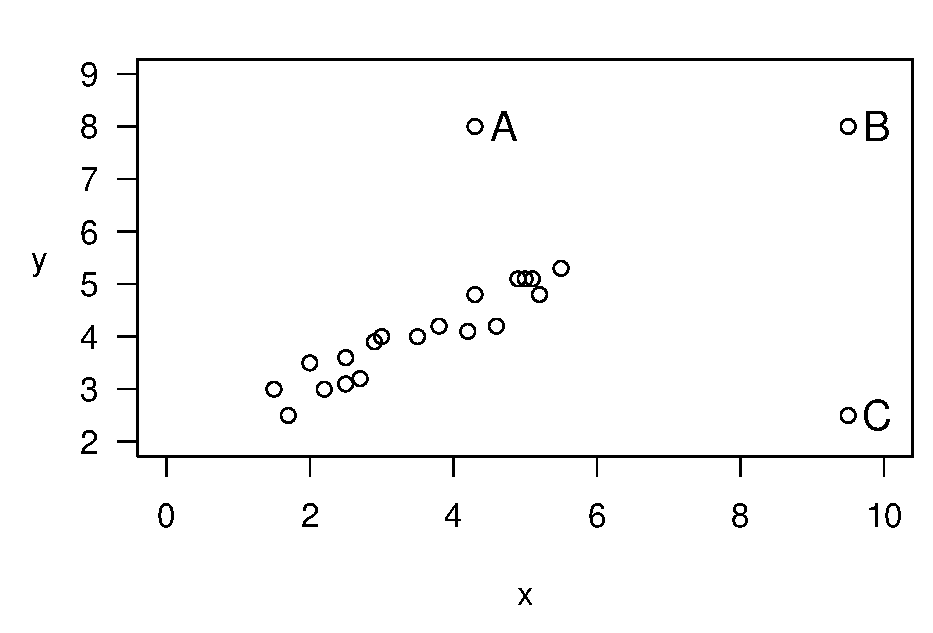
\includegraphics[width=0.6\textwidth]{Chapter2/F2Outlier.eps}
    \caption{\label{F2:Outlier} \small Scatterplot of 19 base plus three unusual points, labeled A, B and C.}
  \end{center}
\end{figure}

To investigate the effect of each type of aberrant point, Table
\ref{T2:OutlierRegression} summarizes the results of four separate
regressions. The first regression is for the nineteen base points.
The other three regressions use the nineteen base points plus each
type of unusual observation.

\begin{table}[h]
\caption{\label{T2:OutlierRegression} Results from Four Regressions}
\begin{tabular}{l|rrrrr}
\hline Data & $b_0$ & $b_1$ & $s$ & $R^2(\%)$ & $t(b_1)$ \\
\hline
19 Base Points & 1.869 & 0.611 & 0.288 & 89.0 & 11.71 \\
19 Base Points ~+~ A & 1.750 & 0.693 & 0.846 & 53.7 & 4.57 \\
19 Base Points ~+~ B & 1.775 & 0.640 & 0.285 & 94.7 & 18.01 \\
19 Base Points ~+~ C & 3.356 & 0.155 & 0.865 & 10.3 & 1.44 \\
\hline
\end{tabular}

\end{table}


Table \ref{T2:OutlierRegression} shows that a regression line
provides a good fit for the nineteen base points. The coefficient of
determination, $R^2$, indicates about 89\% of the variability has
been explained by the line. The size of the typical error, $s$, is
about 0.29, small compared to the scatter in the $y$-values.
Further, the $t$-ratio for the slope coefficient is large.

When the outlier point A is added to the nineteen base points, the
situation deteriorates dramatically. The $R^2$ drops from 89\% to
53.7\% and $s$ increases from about 0.29 to about 0.85. The fitted
regression line itself does not change that much even though our
confidence in the estimates has decreased.

An outlier is unusual in the $y$-value, but ``unusual in the
$y$-value'' depends on the $x$-value. To see this, keep the
$y$-value of Point A the same, but increase the $x$-value and call
the point B.

When the point B is added to the nineteen base points, the
regression line provides a \emph{better} fit. Point B is close to
being on the line of the regression fit generated by the nineteen
base points. Thus, the fitted regression line and the size of the
typical error, $s$, do not change much. However, $R^2$ increases
from 89\% to nearly 95 percent. If we think of $ R^2$ as
$1-(Error~SS)/(Total~SS)$, by adding point B we have increased $
Total~SS$, the total squared deviations in the $y$'s, even though
leaving $ Error~SS$ relatively unchanged. Point B is not an outlier,
but it is a high leverage point.

To show how influential this point is, drop the $y$-value
considerably and call this the new point C. When this point is added
to the nineteen base points, the situation deteriorates
dramatically. The $R^2$ coefficient drops from 89\% to 10\%, and the
$s$ more than triples, from 0.29 to 0.87. Further, the regression
line coefficients change dramatically.

Most users of regression at first do not believe that one point in twenty
can have such a dramatic effect on the regression fit. The fit of a
regression line can always be improved by removing an outlier. If the point
is a high leverage point and not an outlier, it is not clear whether the fit
will be improved when the point is removed.

\linejed

Simply because you can dramatically improve a regression fit by
omitting an observation does not mean you should always do so! The
goal of data analysis is to understand the information in the data.
Throughout the text, we will encounter many data sets where the
unusual points provide some of the most interesting information
about the data. The goal of this subsection is to recognize the
effects of unusual points; Chapter 5 will provide options for
handling unusual points in your analysis.

All quantitative disciplines, such as accounting, economics, linear
programming, and so on, practice the art of \emph{sensitivity analysis}.
Sensitivity analysis is a description of the global changes in a system due
to a small local change in an element of the system. Examining the effects
of individual observations on the regression fit is a type of sensitivity
analysis.

\newpage

\linejed

\textbf{Example: Lottery Sales -- Continued.} Figure
\ref{F2:PlotWithKenosha} exhibits an outlier; the point in the upper
left-hand side of the plot represents a zip code that includes
Kenosha, Wisconsin. Sales for this zip code are unusually high given
its population. Kenosha is close to the Illinois border; residents
from Illinois probably participate in the Wisconsin lottery thus
effectively increasing the potential pool of sales in Kenosha. Table
\ref{T2:RegressionKenosha} summarizes the regression fit both with
and without this zip code.

\begin{table}[h]
\caption{\label{T2:RegressionKenosha} Regression Results with and
without Kenosha}

\begin{tabular}{l|rrrrr}
 \hline
Data & $b_0$ & $b_1$ & $s$ & $R^2(\%)$ & $t(b_1)$ \\ \hline
With Kenosha & 469.7 & 0.647 & 3,792 & 78.5 & 13.26 \\
Without Kenosha & -43.5 & 0.662 & 2,728 & 88.3 & 18.82 \\ \hline
\end{tabular}

\end{table}

\begin{figure}[htp]
  \begin{center}
    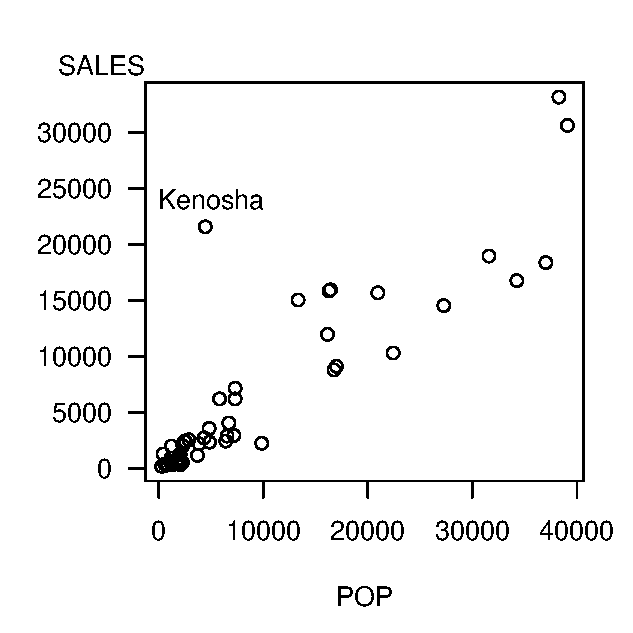
\includegraphics[width=0.6\textwidth]{Chapter2/F2PlotWithKenosha.eps}
    \caption{\label{F2:PlotWithKenosha} \small Scatter plot
of SALES versus POP, with the outlier corresponding to Kenosha
marked.}
  \end{center}
\end{figure}

For the purposes of inference about the slope, the presence of
Kenosha does not alter the results dramatically. Both slope
estimates are qualitatively similar and the corresponding
$t$-statistics are very high, well above cut-offs for statistical
significance. However, there are dramatic differences when assessing
the quality of the fit. The coefficient of determination, $R^2$,
increased from 78.5\% to 88.3\% when deleting Kenosha. Moreover, our
``typical deviation'' $s$ dropped by over \$1,000. This is
particularly important if we wish to tighten our prediction
intervals.

To check the accuracy of our assumptions, it is also customary to
check the normality assumption. One way of doing this is the $qq$
plot, introduced in Section 1.2. The two panels in Figures
\ref{F2:QQplotsKenosha} are $qq$ plots with and without the Kenosha
zip code. Recall that points ``close'' to linear indicate
approximate normality. In the right-hand panel of Figure
\ref{F2:QQplotsKenosha}, the sequence does appear to be linear so
that residuals are approximately normally distributed. This is not
the case in the left-hand panel, where the sequence of points
appears to climb dramatically for large quantiles. The interesting
thing is that the non-normality of the distribution is due to a
single outlier, not a pattern of skewness that is common to all the
observations.

\begin{figure}[htp]
  \begin{center}
    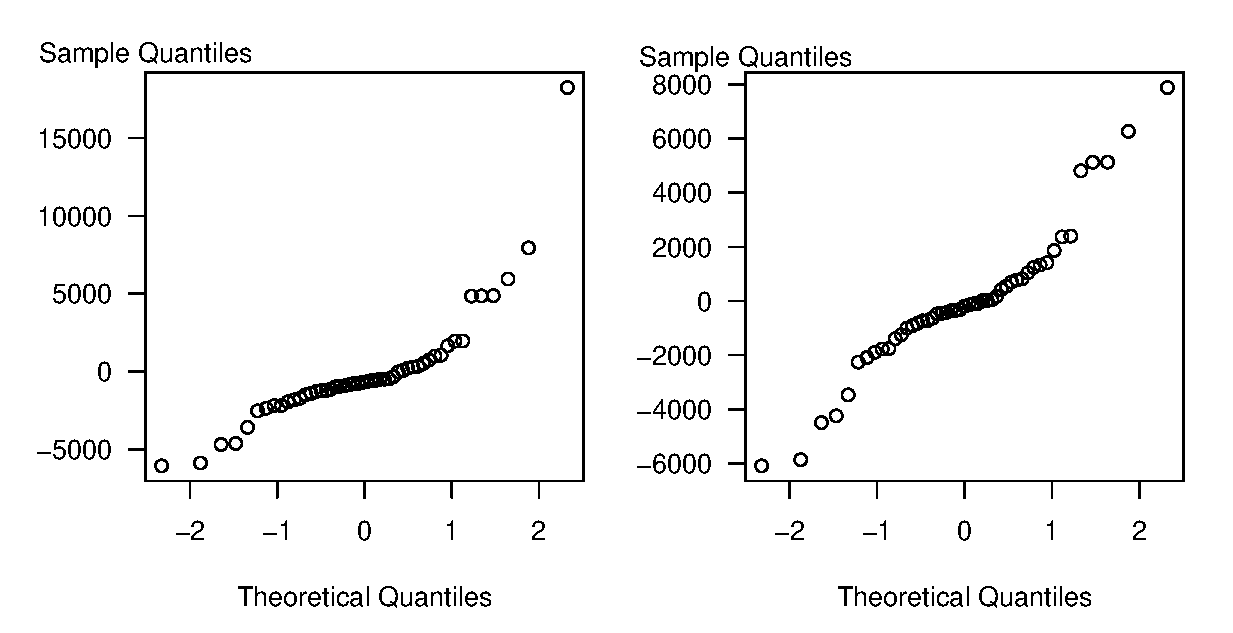
\includegraphics[width=1\textwidth]{Chapter2/F2QQplotsKenosha.eps}
    \caption{\label{F2:QQplotsKenosha} \small $qq$ Plots of Wisconsin Lottery Residuals.
    The left-hand panel is based on all 50 points.
The right-hand panel is based on 49 points, residuals from a
regression after removing Kenosha.}
  \end{center}
\end{figure}

\linejed

\section{Application: Capital Asset Pricing Model}\label{S2:CAPM}\ecaptionjed{Capital Asset Pricing Model}
\index{actuarial \& financial terms and concepts!capital asset
pricing model, CAPM}

In this section, we study a financial application, the Capital Asset
Pricing Model, often referred to by the acronym CAPM. The name is
something of a misnomer in that the model is really about
\emph{returns} based on capital assets, not the prices themselves.
The types of assets that we examine are equity securities that are
traded on an active market, such as the New York Stock Exchange
(NYSE). For a stock on the exchange, we can relate returns to prices
through the following expression:

\scalefont{0.9}
\begin{equation*}
\mathrm{return=}\frac{\mathrm{
price~at~the~end~of~a~period+dividends-price~at~the~beginning~of~a~period}}{
\mathrm{price~at~the~beginning~of~a~period}}.
\end{equation*}
\scalefont{1.1111}

If we can estimate the returns that a stock generates, then
knowledge of the price at the beginning of a generic financial
period allows us to estimate the value at the end of the period
(ending price plus dividends). Thus, we follow standard practice and
model returns of a security.

An intuitively appealing idea, and one of the basic characteristics
of the CAPM, is that there should be a relationship between the
performance of a security and the market. One rationale is simply
that if economic forces are such that the market improves, then
those same forces should act upon an individual stock, suggesting
that it also improve. As noted above, we measure performance of a
security through the return. To measure performance of the market,
several market indices exist that summarize the performance of each
exchange. We will use the ``equally-weighted'' index of the Standard
\& Poor's 500. The Standard \& Poor's 500 is the collection of the
500 largest companies traded on the NYSE, where ``large'' is
identified by Standard \& Poor's, a financial services rating
organization. The equally-weighted index is defined by assuming a
portfolio is created by investing one dollar in each of the 500
companies.

Another rationale for a relationship between security and market
returns comes from financial economics theory. This is the CAPM
theory, attributed to Sharpe (1964) and Lintner (1965) and based on
the portfolio diversification ideas of Harry Markowitz (1959). Other
things equal, investors would like to select a return with a high
expected value and low standard deviation, the latter being a
measure of risk. One of the desirable properties about using
standard deviations as a measure of riskiness is that it is
straight-forward to calculate the standard deviation of a portfolio.
One only needs to know the standard deviation of each security and
the correlations among securities. A notable security is a risk-free
one, that is, a security that theoretically has a zero standard
deviation. Investors often use a 30-day U.S. Treasury bill as an
approximation of a risk-free security, arguing that the probability
of default of the U.S. government within 30 days is negligible.
Positing the existence of a risk-free asset and some other mild
conditions, under the CAPM theory there exists an efficient frontier
called the \emph{securities market line}. This frontier specifies
the minimum expected return that investors should demand for a
specified level of risk. To estimate this line, we can use the
equation\index{actuarial \& financial terms and concepts!securities
market line}
\begin{equation*}
\mathrm{E}~r = \beta_0 + \beta_1 r_m
\end{equation*}
where $r$ is the security return and $r_m$ is the market return. We
interpret $\beta_1 r_m$ as a measure of the amount of security
return that is attributed to the behavior of the market.

Testing economic theory, or models arising from any discipline, involves
collecting data. The CAPM theory is about ex-ante (before the fact) returns
even though we can only test with ex-post (after the fact) returns. Before
the fact, the returns are unknown and there is an entire distribution of
returns. After the fact, there is only a single realization of the security
and market return. Because at least two observations are required to
determine a line, CAPM models are estimated using security and market data
gathered over time. In this way, several observations can be made. For the
purposes of our discussions, we follow standard practice in the securities
industry and examine monthly prices.

\subsubsection*{Data}

\empexjed{CAPM}\index{datasets!capital asset pricing model}

To illustrate, consider monthly returns over the five year period
from January, 1986 to December, 1990, inclusive. Specifically, we
use the security returns from the Lincoln National Insurance
Corporation as the dependent variable ($y$) and the market returns
from the index of the Standard \& Poor's 500 Index as the
explanatory variable ($x$). At the time, the Lincoln was a large,
multi-line, insurance company, headquartered in the midwest of the
U.S., specifically in Fort Wayne, Indiana. Because it was well known
for its' prudent management and stability, it is a good company to
begin our analysis of the relationship between the market and an
individual stock.

We begin by interpreting some of basic summary statistics, in Table
\ref{T2:SumStatsCAPM}, in terms of financial theory. First, an
investor in the Lincoln will be concerned that the five year average
return, $\overline{y}=0.00510$, is below the return of the market,
$\overline{x}=0.00741$. Students of interest theory recognize that
monthly returns can be converted to an annual basis using geometric
compounding. For example, the annual return of the Lincoln is
$(1.0051)^{12}-1=0.062946$, or roughly 6.29 percent. This is
compared to an annual return of 9.26\% (= (1$00((1.00741)^{12}-1$))
for the market. A measure of risk, or volatility, that is used in
finance is the standard deviation. Thus, interpret $s_y$ = 0.0859
$>$ 0.05254 = $s_x$ to mean that an investment in the Lincoln is
riskier than that of the market. Another interesting aspect of Table
\ref{T2:SumStatsCAPM} is that the smallest market return, -0.22052,
is 4.338 standard deviations below its average
((-0.22052-0.00741)/0.05254 = -4.338). This is highly unusual with
respect to a normal distribution.

\begin{table}[h]
\caption{\label{T2:SumStatsCAPM} Summary Statistics of 60 Monthly
Observations}
\begin{tabular}{c|ccccc}
\hline
& & & Standard &  \\
&  Mean & Median & Deviation & Minimum & Maximum\\ \hline
LINCOLN & 0.0051 & 0.0075 & 0.0859 & -0.2803 & 0.3147 \\
MARKET & 0.0074 & 0.0142 & 0.0525 & -0.2205 & 0.1275 \\ \hline
\multicolumn{6}{c}{\textit{Source: Center for Research on Security
Prices, University of Chicago}} \\ \hline
\end{tabular}
\end{table}

We next examine the data over time, as is given graphically in
Figure \ref{F2:TimeSeriesPlots}. These are scatter plots of the
returns versus time, called \emph{time series plots}. In Figure
\ref{F2:TimeSeriesPlots}, one can clearly see the smallest market
return and a quick glance at the horizontal axis reveals that this
unusual point is in October, 1987, the time of the well-known market
crash.


\begin{figure}[htp]
  \begin{center}
    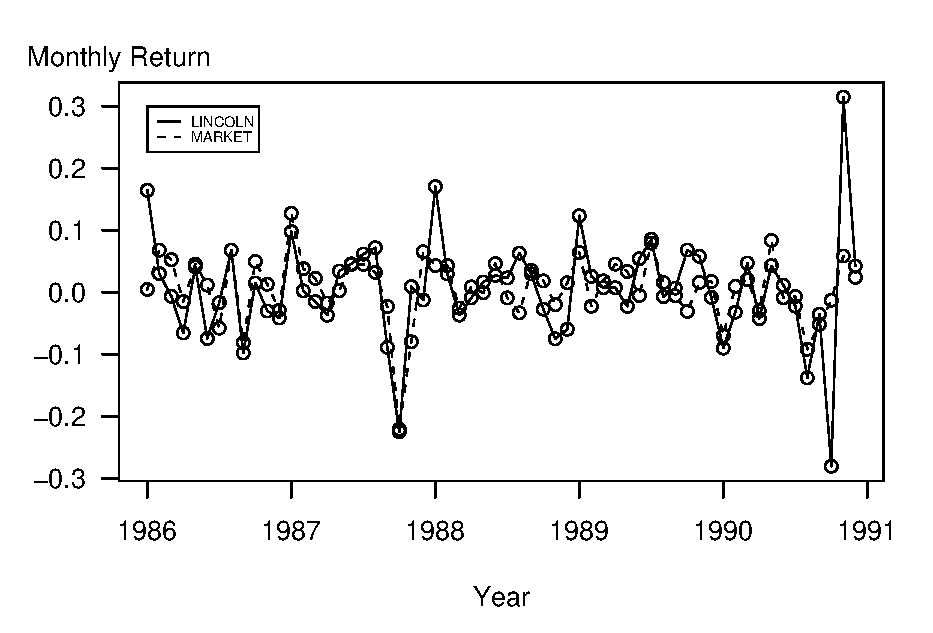
\includegraphics[width=0.8\textwidth]{Chapter2/F2TimeSeriesPlots.eps}
    \caption{\label{F2:TimeSeriesPlots} \small Time series
plot of returns from the Lincoln National Corporation and the
market. There are 60 monthly returns over the period January, 1986
through December, 1990.}
  \end{center}
\end{figure}


\bigskip

The scatter plot in Figure \ref{F2:LincolnvsMarket} graphically
summarizes the relationship between Lincoln's return and the return
of the market. The market crash is clearly evident in Figure
\ref{F2:LincolnvsMarket} and represents a high leverage point. With
the regression line (described below) superimposed, the two outlying
points that can be seen in Figure \ref{F2:TimeSeriesPlots} are also
evident. Despite these anomalies, the plot in Figure
\ref{F2:LincolnvsMarket} does suggest that there is a linear
relationship between Lincoln and market returns.



\begin{figure}[htp]
  \begin{center}
    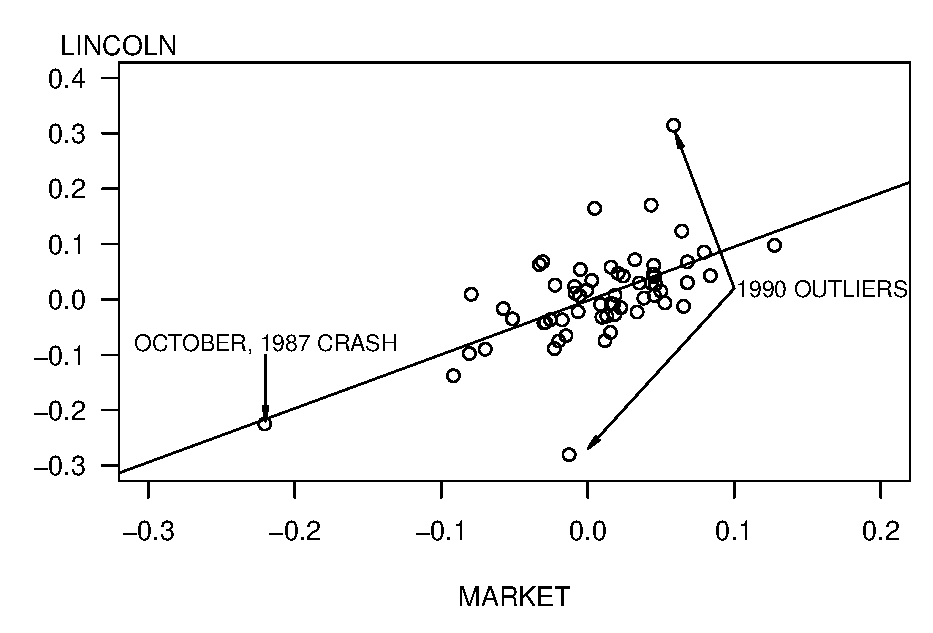
\includegraphics[width=0.8\textwidth]{Chapter2/F2LincolnvsMarket.eps}
    \caption{\label{F2:LincolnvsMarket} \small Scatterplot of Lincoln's return versus the S\&P 500 Index return. The
regression line is superimposed, enabling us to identify the market
crash and two outliers.}
  \end{center}
\end{figure}

\bigskip

\subsubsection*{Unusual Points}

To summarize the relationship between the market and Lincoln's
return, a regression model was fit. The fitted regression is
\begin{equation*}
\widehat{LINCOLN}=-0.00214+0.973 MARKET.
\end{equation*}
The resulting estimated standard error, $s$ = 0.0696 is lower than
the standard deviation of Lincoln's returns, $s_y=0.0859$. Thus, the
regression model explains some of the variability of Lincoln's
returns. Further, the $t$-statistic associated with the slope $b_1$
turns out to be $t(b_1)=5.64$, which is significantly large. One
disappointing aspect is that the statistic $R^2=35.4\%$ can be
interpreted as saying that the market explains only a little over a
third of the variability. Thus, even though the market is clearly an
important determinant, as evidenced by the high $t$-statistic, it
provides only a partial explanation of the performance of the
Lincoln's returns.

In the context of the market model, we may interpret the standard
deviation of the market, $s_x$, as \emph{non-diversifiable risk}.
Thus, the risk of a security can be decomposed into two components,
the diversifiable component and the market component, which is
non-diversifiable. The idea here is that by combining several
securities we can create a portfolio of securities that, in most
instances, will reduce the riskiness of our holdings when compared
with a single security. Again, the rationale for holding a security
is that we are compensated through higher expected returns by
holding a security with higher riskiness. To quantify the relative
riskiness, it is not hard to show that
\begin{equation}
s_y^2 = b_1^2 s_x^2 + s^2 \frac{n-2}{n-1}.
\end{equation}

The riskiness of a security is due to the riskiness due to the
market plus the riskiness due to a diversifiable component. Note
that the riskiness due to the market component, $s_x^2$, is larger
for securities with larger slopes. For this reason, investors think
of securities with slopes $b_1$ greater than one as ``aggressive''
and slopes less than one as ``defensive.''

\subsubsection*{Sensitivity Analysis}

The above summary immediately raises two additional issues. First,
what is the effect of the October, 1987 crash on the fitted
regression equation? We know that unusual observations, such as the
crash, may potentially influence the fit a great deal. To this end,
the regression was re-run without the observation corresponding to
the crash. The motivation for this is that the October 1987 crash
represents a combination of highly unusual events (the interaction
of several automated trading programs operated by the large stock
brokerage houses) that we do not wish to represent using the same
model as our other observations. Deleting this observation, the
fitted regression is
\begin{equation*}
\widehat{LINCOLN} = -0.00181 + 0.956 MARKET,
\end{equation*}
with $R^2=26.4\%$, $t(b_1)=4.52$, $s=0.0702$ and $s_y=0.0811$. We
interpret these statistics in the same fashion as the fitted model
including the October 1987 crash. It is interesting to note,
however, that the proportion of variability explained has actually
\emph{decreased} when excluding the influential point. This serves
to illustrate an important point. High leverage points are often
looked upon with dread by data analysts because they are, by
definition, unlike other observations in the data set and require
special attention. However, when fitting relationships among
variables, they also represent an opportunity because they allow the
data analyst to observe the relationship between variables over
broader ranges than otherwise possible. The downside is that these
relationships may be nonlinear or follow an entirely different
pattern when compared to the relationships observed in the main
portion of the data.

The second question raised by the regression analysis is what can be
said about the unusual circumstances that gave rise to the unusual
behavior of Lincoln's returns in October and November of 1990. A
useful feature of regression analysis is to identify and raise the
question; it does not resolve it. Because the analysis clearly
pinpoints two highly unusual points, it suggests to the data analyst
to go back and ask some specific questions about the sources of the
data. In this case, the answer is straightforward. In October of
1990, the Travelers' Insurance Company, a competitor, announced that
it would take a large write-off in their real estate portfolio. due
to an unprecedented number of mortgage defaults. The market reacted
quickly to this news, and investors assumed that other large stock
life insurers would also soon announce large write-offs.
Anticipating this news, investors tried to sell their portfolios of,
for example, Lincoln's stock, thus causing the price to plummet.
However, it turned out that investors overreacted to this news and
that Lincoln's portfolio of real estate was indeed sound. Thus,
prices quickly returned to their historical levels.

\section{Illustrative Regression Computer Output}

Computers and statistical software packages that perform specialized
calculations play a vital role in modern-day statistical analyses.
Inexpensive computing capabilities have allowed data analysts to
focus on relationships of interest. Specifying models that are
attractive merely for their computational simplicity is much less
important now compared to times before the widespread availability
of inexpensive computing. An important theme of this text is to
focus on relationships of interest and to rely on widely available
statistical software to estimate the models that we specify.

With any computer package, generally the most difficult parts of operating
the package are the (i) input, (ii) using the commands and (iii)
interpreting the output. You will find that most modern statistical software
packages accept spreadsheet or text-based files, making input of data
relatively easy. Personal computer statistical software packages have
menu-driven command languages with easily accessible on-line help
facilities. Once you decide what to do, finding the right commands is
relatively easy.

This section provides guidance in interpreting the output of
statistical packages. Most statistical packages generate similar
output. Below, three examples of standard statistical software
packages, EXCEL, SAS and R are given. The annotation symbol
``\lbrack .]'' marks a statistical quantity that is described in the
legend. Thus, this section provides a link between the notation used
in the text and output from some of the standard statistical
software packages.

\scalefont{0.8}

\bigskip

\noindent \rule{5.5in}{0.03in}

\bigskip

{\textbf{EXCEL Output}}

\begin{alltt}
Regression Statistics
Multiple R              0.886283[F]
R Square                0.785497[k]
Adjusted R Square       0.781028[l]
Standard Error          3791.758[j]
Observations              50[a]

ANOVA
           df              SS          MS             F     Significance F
Regression   1[m]   2527165015 [p]  2527165015 [s]  175.773[u]   1.15757E-17[v]
Residual    48[n]   690116754.8[q]  14377432.39[t]
Total       49[o]   3217281770 [r]

        Coefficients    Standard Error      t Stat         P-value
Intercept    469.7036[b] 702.9061896[d]   0.668230846[f] 0.507187[h]
X Variable 1 0.647095[c] 0.048808085[e]   13.25794257[g] 1.16E-17[i]

\end{alltt}

\noindent \rule{5.5in}{0.03in}

\newpage
\noindent \rule{5.5in}{0.03in}

\bigskip

{\textbf{SAS Output}}

\begin{alltt}
                          The SAS System
                         The REG Procedure
                    Dependent Variable: SALES

                        Analysis of Variance
                               Sum of           Mean
Source                   DF        Squares         Square     F Value      Pr > F
Model                  1[m]   2527165015[p]   2527165015[s]   175.77[u]    <.0001[v]
Error                 48[n]    690116755[q]     14377432[t]
Corrected Total       49[o]   3217281770[r]

        Root MSE           3791.75848[j]    R-Square     0.7855[k]
        Dependent Mean     6494.82900[H]    Adj R-Sq     0.7810[l]
        Coeff Var            58.38119[I]

                        Parameter Estimates
                           Parameter       Standard
Variable     Label        DF     Estimate        Error      t  Value    Pr > |t|
Intercept    Intercept     1   469.70360[b]  702.90619[d]    0.67[f]    0.5072[h]
POP          POP           1     0.64709[c]    0.04881[e]   13.26[g]    <.0001[i]
\end{alltt}

\noindent \rule{5.5in}{0.03in}

\bigskip

{\textbf{R Output}}

\begin{alltt}
Analysis of Variance Table

Response: SALES
          Df     Sum Sq      Mean Sq        F value         Pr(>F)
POP        1[m] 2527165015[p] 2527165015[s] 175.77304[u] <2.22e-16[v]***
Residuals 48[n]  690116755[q]   14377432[t]
---
Call: lm(formula = SALES ~ POP)

Residuals:
   Min     1Q Median     3Q    Max
 -6047  -1461   -670    486  18229

Coefficients:
            Estimate     Std. Error t value     Pr(>|t|)
(Intercept) 469.7036[b] 702.9062[c]  0.67[f]    0.51     [h]
POP           0.6471[c]   0.0488[e] 13.26[g]   <2e-16 ***[i]
---
Signif. codes:  0 �***� 0.001 �**� 0.01 �*� 0.05 �.� 0.1 � � 1

Residual standard error: 3790[j] on 48[n] degrees of freedom
Multiple R-Squared: 0.785[k],      Adjusted R-squared: 0.781[l]
F-statistic:  176[u] on 1[m] and 48[n] DF,  p-value: <2e-16[v]
\end{alltt}

\noindent \rule{5.5in}{0.03in} \scalefont{1.25}



\newpage \textbf{Legend Annotation Definition, Symbol }
\index{symbols!$n$, sample size}\index{symbols!$b_0$, least squares
intercept}\index{symbols!$b_1$, least squares
slope}\index{symbols!$se(b)$, standard error of $b$}
\index{symbols!$t(b)$, $t$-ratio for $b$}\index{symbols!$p$-value,
probability value}\index{symbols!$R^2$, coefficient of
determination} \index{symbols!$s^2$, mean square error}
\index{symbols!$s$, residual standard
deviation}\index{symbols!$R_a^2$, coefficient of determination
adjusted for degrees of freedom}

\begin{multicols}{2}

\scalefont{0.9}

[a] Number of observations $n$.

[b] The estimated intercept $b_0$.

[c] The estimated slope $b_1$.

[d] The standard error of the intercept, $se(b_0)$.

[e] The standard error of the intercept, $se(b_1)$.

[f] The $t$-ratio associated with the intercept, $t(b_0) =
b_0/se(b_0)$.

[g] The $t$-ratio associated with the slope, $t(b_1) = b_1/se(b_1)$.

[h] The $p$-value associated with the intercept; here, $
p-value=Pr(|t_{n-2}|>|t(b_0)|)$, where $t(b_0)$ is the realized
value (0.67 here) and $t_{n-2}$ has a $t$-distribution with
$df=n-2$.

[i] The $p$-value associated with the slope; here, $
p-value=Pr(|t_{n-2}|>|t(b_1)|)$, where $t(b_1)$ is the realized
value (13.26 here) and $t_{n-2}$ has a $t$-distribution with $
df=n-2 $.

[j] The residual standard deviation, $s$.

[k] The coefficient of determination, $R^2$.

[l] The coefficient of determination adjusted for degrees of
freedom, $R_{a}^2$. (This term will be defined in Chapter 3.)

[m] Degree of freedom for the regression component. This is 1 for
one explanatory variable.

[n] Degree of freedom for the error component, $n-2$, for regression
with one explanatory variable.

[o] Total degrees of freedoms, $n-1$.

[p] The regression sum of squares, $Regression~SS$.

[q] The error sum of squares, $Error~SS$.

[r] The total sum of squares, $Total~SS$.

\index{symbols!$Error~SS$, error sum of
squares}\index{symbols!$Regression~SS$, regression sum of
squares}\index{symbols!$Total~SS$, total sum of squares}


[s] The regression mean square, $Regression~MS = Regression~SS/1$,
for one explanatory variable.

[t] The error mean square, $s^2=Error~MS = Error~SS/(n-2)$, for one
explanatory variable.

[u] The $F-ratio=(Regression~MS)/(Error~MS)$. (This term will be defined in
Chapter 3.)

[v] The $p$-value associated with the $F-ratio$. (This term will be defined
in Chapter 3.)

[w] The observation number, $i$.

[x] The value of the explanatory variable for the $i$th observation,
$x_i$.

[y] The response for the $i$th observation, $y_i$.

[z] The fitted value for the $i$th  observation, $\widehat{y}_i$.

[A] The standard error of the fit, $se(\widehat{y}_i)$.

[B] The residual for the $i$th observation, $e_i$.

[C] The standardized residual for the $i$th  observation,
$e_i/se(e_i)$. The standard error $se(e_i)$ will be defined in
Section 5.3.1.

[F] The multiple correlation coefficient is the square root of the
coefficient of determination, $R=\sqrt{R^2}$. This will be defined
in Chapter 3.

[G] The standardized coefficient is $b_1s_x/s_y$ For regression with
one explanatory variable, this is equivalent to $r$, the correlation
coefficient.

[H] The average response, $\overline{y}$.

[I] The coefficient of variation of the response is
$s_y/\overline{y}$. SAS prints out $100s_y/\overline{y}$ .

\scalefont{1.1111}

\end{multicols}


\section{Further Reading and References}

Relatively few applications of regression are basic in the sense
that they use only one explanatory variable; the purpose of
regression analysis is to reduce complex relationships among many
variables. Section \ref{S2:CAPM} described an important exception to
this general rule, the CAPM finance model; see Panjer et al. (1998)
for additional actuarial descriptions of this model. Campbell et al.
(1997) gives a financial econometrics perspective.

\bigskip

\newpage

\textbf{Chapter References}

\begin{multicols}{2}

\scalefont{0.9}

Anscombe, Frank (1973). Graphs in statistical analysis. \textit{The
American Statistician} 27, 17-21.

Campbell, John Y., Andrew W. Lo and A. Craig MacKinlay (1997).
\textit{The Econometrics of Financial Markets}. Princeton University
Press, Princeton, New Jersey.

Frees, Edward W. and Tom W. Miller (2003). Sales forecasting using
longitudinal data models. \textit{International Journal of
Forecasting} 20, 97-111.

Goldberger, Arthur (1991). \textit{A Course in Econometrics}.
Harvard University Press, Cambridge.

Koch, Gary J. (1985). A basic demonstration of the [-1, 1] range for
the correlation coefficient. \textit{American Statistician} 39,
201-202.

Linter, J. (1965). The valuation of risky assets and the selection
of risky investments in stock portfolios and capital budgets.
\textit{Review of Economics and Statistics}, 13-37.

Manistre, B. John and Geoffrey H. Hancock (2005). Variance of the
CTE estimator. \textit{North American Actuarial Journal} 9(2),
129-156.

Markowitz, Harry (1959). \textit{Portfolio Selection: Efficient
Diversification of Investments}. John Wiley, New York.

Panjer, Harry H., Phelim P. Boyle, Samuel H. Cox, Daniel Dufresne,
Hans U. Gerber, Heinz H. Mueller, Hal W. Pedersen, Stanley R.
Pliska, Michael Sherris, Elias S. Shiu and Ken S. Tan (1998).
\textit{Financial Economics: With Applications to Investment,
Insurance and Pensions}. Society of Actuaries, Schaumburg, Illinois.

Pearson, Karl (1895). \textit{Royal Society Proceedings} 58, 241.

Serfling, Robert J. (1980). \textit{Approximation Theorems of
Mathematical Statistics}. John Wiley and Sons, New York.

Sharpe, William F. (1964). Capital asset prices: A theory of market
equilibrium under risk. \textit{Journal of Finance}, 425-442.

Stigler, Steven M. (1986). \textit{The History of Statistics:  The
Measurement of Uncertainty before 1900}. Harvard University Press,
Cambridge, MA.

\scalefont{1.1111}

\end{multicols}


\section{Exercises}

\scalefont{0.90}

\begin{exercises}

\subsection*{Sections 2.1-2.2}

\item Consider the following data set~~
\begin{tabular}{l|ccc}
\hline
$i$ & 1 & 2 & 3 \\
$x_i$ & 2 & -6 & 7 \\
$y_i$ & 3 & 4 & 6\\ \hline
\end{tabular}.

Fit a regression line using the method of least squares. Determine
$r$, $b_1$ and $b_0$.

\item \label{Ex:ZeroCorr} \textbf{A perfect relationship, yet zero correlation.} Consider the
quadratic relationship $y=x^2$, with data $
\begin{tabular}{l|rrrrr}
\hline
$i$ & 1 & 2 & 3 & 4 & 5 \\
$x_i$ & -2 & -1 & 0 & 1 & 2 \\
$y_i$ & 4 & 1 & 0 & 1 & 4 \\ \hline
\end{tabular}.$

a. Produce a rough graph for this data set.

b. Check that the correlation coefficient is $r=0$.


\item \textbf{Boundedness of the correlation coefficient.} Use the
following steps to show that $r$ is bounded by -1 and 1 (These steps
are due to Koch, 1990).

a. Let $a$ and $c$ be generic constants. Verify
\begin{eqnarray*}
0 & \leq & \frac{1}{n-1}\sum_{i=1}^{n}\left(
a\frac{x_i-\overline{x}}{s_x}-c
\frac{y_i-\overline{y}}{s_y}\right) ^2 \\
&=& a^2+c^2-2acr.
\end{eqnarray*}

b. Use the results in part (a) to show $2ac(r-1)\leq (a-c)^2.$

c. By taking $a=c$, use the result in part (b) to show $r\leq 1$.

d. By taking $a=-c$, use the results in part (b) to show $r\geq -1$.

e. Under what conditions is $r=-1$? Under what conditions is $r=1$?


\item \textbf{Regression coefficients are weighted sums.} Show that
the intercept term, $b_0$, can be expressed as a weighted sum of the
dependent variables. That is, show that
$b_0=\sum_{i=1}^{n}w_{i,0}y_i.$ Further, express the weights in
terms of the slope weights, $w_i$.

\item \textbf{Another expression for the slope as a weighted sum}

a. Using algebra, establish an alternative expression
\begin{equation*}
b_1=\frac{\sum_{i=1}^{n}weight_i~slope_i}{ \sum_{i=1}^{n}weight_i}.
\end{equation*}
Here, $slope_i$ is the slope between $(x_i,y_i)$ and
$(\bar{x},\bar{y})$. Give a precise form for the weight $weight_i$
as a function of the explanatory variable $x$.

b. Suppose that $\bar{x} = 4,\bar{y} = 3, x_1 = 2 \mathrm{~and~} y_1
= 6$. Determine the slope and weight for the first observation, that
is, $slope_1$ and $weight_1$.


\item Consider two variables, $y$ and $x$. Do a regression
of $y$ on $x$ to get a slope coefficient which we call $b_{1,x,y}$.
Do another regression of $x$ on $y$ to get a slope coefficient which
we call $b_{1,y,x}$. Show that the correlation coefficient between
$x$ and $y$ is the geometric mean of the two slope coefficients up
to sign, that is, show that $|r|=\sqrt{ b_{1,x,y}b_{1,y,x}}.$

\item \textbf{Regression through the origin.} Consider the model
$y_i=\beta_1 x_i + \varepsilon _i$, that is, regression with one
explanatory variable \emph{without} the intercept term. This model
is called \emph{regression through the origin} because the true
regression line $\mathrm{E}y = \beta_1 x$ passes through the origin
(the point (0, 0)). For this model, the least squares estimate of
$\beta_1$ is that number $b_1$ that minimizes the sum of squares
$\mathrm{SS}(b_1^{\ast} )=\sum_{i=1}^{n}\left( y_i -
b_1^{\ast}x_i\right) ^2.$

a. Verify that
\begin{equation*}
b_1 = \frac{\sum_{i=1}^{n} x_i y_i}{\sum_{i=1}^{n}x_i^2}.
\end{equation*}

b. Consider the model $y_i=\beta_1 z_i^2 + \varepsilon _i$, a
quadratic model passing through the origin. Use the result of part
(a) to determine the least squares estimate of $\beta_1$.

\item \label{Ex:SimpleBLR} a. Show that
\begin{equation*}
s_y^2=\frac{1}{n-1}\sum_{i=1}^{n}\left( y_i-\overline{y}\right) ^2=
\frac{1}{n-1}\left( \sum_{i=1}^{n}y_i^2-n\overline{y}^2\right) .
\end{equation*}

b. Follow the same steps to show $\sum_{i=1}^{n}\left( y_i -
\overline{y} \right) \left( x_i-\overline{x}\right) =\sum_{i=1}^{n}
x_i y_i - n \overline{x}~\overline{y}.$

c. Show that
\begin{equation*}
b_{1}=\frac{\sum_{i=1}^{n}\left( y_i-\overline{y}\right) \left( x_i-
\overline{x}\right) }{\sum_{i=1}^{n}\left( x_i - \overline{x}
\right) ^2}
\end{equation*}

d. Establish the commonly used formula
\begin{equation*}
b_{1}=\frac{\sum_{i=1}^{n}x_iy_i-n\overline{x}~\overline{y}}{\sum_{i=1}^{n}x_i^2
- n\overline{x}^2}.
\end{equation*}

\index{categorical variable!binary}
\item \textbf{Interpretation of coefficients associated with a binary
explanatory variable.}\label{Ex:TwoPoPSLR} Suppose that $x_i$ only
takes on the values 0 and 1. Out of the $n$ observations, $n_1$ take
on the value $x=0$. These $n_1 $ observations have an average $y$
value of $\overline{y}_1$. the remaining $n-n_1$ observations have
value $x=1$ and an average $y$ value of $\overline{y}_2$. Use
Exercise 2.\ref{Ex:SimpleBLR} to show that $b_1 = \overline{y}_2 -
\overline{y}_1.$

\newpage

\empexjed{WiscNursingHome}\index{datasets!nursing home utilization}

\item \textbf{Nursing Home Utilization.}\label{Ex:NursHome2a}
This exercise considers nursing home data provided by the Wisconsin
Department of Health and Family Services (DHFS) and described in
Exercise 1.\ref{Ex:NursHome}.

\textbf{Part 1:} Use cost report year 2000 data, and do the
following analysis.

a. Correlations

a(i). Calculate the correlation between TPY and LOGTPY. Comment on
your result.

a(ii). Calculate the correlation among TPY, NUMBED and SQRFOOT. Do
these variables appear highly correlated?

a(iii). Calculate the correlation between TPY and NUMBED/10. Comment
on your result.

b. Scatter plots. Plot TPY versus NUMBED and TPY versus SQRFOOT.
Comment on the plots.

c. Basic linear regression.

c(i). Fit a basic linear regression model using TPY as the outcome
variable and NUMBED as the explanatory variable. Summarize the fit
by quoting the coefficient of determination, $R^2$, and the
$t$-statistic for NUMBED.

c(ii). Repeat c(i), using SQRFOOT instead of NUMBED. In terms of
$R^2$, which model fits better?

c(iii). Repeat c(i), using LOGTPY for the outcome variable and
LOG(NUMBED) as the explanatory variable.

c(iv). Repeat c(iii), using LOGTPY for the outcome variable and
LOG(SQRFOOT) as the explanatory variable.

\textbf{Part 2:} Fit the model in Part 1.c(1) using 2001 data. Are
the patterns stable over time?


\subsection*{Sections 2.3-2.4}

\item Suppose that, for a sample size of $n$ = 3, you have $
e_2$ = 24 and $e_{3}$ = -1. Determine $e_{1}$.

\item Suppose that $r=0$, $n=15$ and $s_y = 10$. Determine
$s$.

\item \textbf{The correlation coefficient and
the coefficient of determination.}\label{Ex:Chap2Corr}  Use the
following steps to establish a relationship between the coefficient
of determination and the correlation coefficient.

a. Show that $\widehat{y}_i-\overline{y}=b_1(x_i-\overline{x}).$

b. Use part (a) to show that $Regress~SS=$ $\sum_{i=1}^{n}\left(
\widehat{y}_i - \overline{y} \right)^2 = b_1^2s_x^2(n-1).$

c. Use part (b) to establish $R^2=r^2.$

\item \label{Ex:AverageResid} Show that the average residual is zero, that is, show
that $n^{-1}\sum_{i=1}^{n} e_i=0.$

\item \textbf{Correlation between residuals and explanatory variables.}
Consider a generic sequence of pairs of numbers ($x_1,y_1$), ...,
($x_n,y_n$) with the correlation coefficient computed as \
$r(y,x)=\left[ (n-1)s_ys_x\right] ^{-1}\sum_{i=1}^{n}\left(
y_i-\overline{y}\right) \left( x_i-\overline{x}\right) .$

a. Suppose that either $\overline{y}=0,\overline{x}=0$ or both
$\overline{x}$ \ and $\overline{y}=0.$ Then, check that $r(y,x)=0$
implies $\sum_{i=1}^{n}y_i x_i=0$\ and vice-versa.

b. Show that the correlation between the residuals and the
explanatory variables is zero. Do this by using part (a) of Exercise
2.13 to show that $\sum_{i=1}^{n} x_i e_i = 0$ and then apply part
(a).

c. Show that the correlation between the residuals and fitted values
is zero. Do this by showing that $\sum_{i=1}^n \widehat{y}_i e_i =
0$ \ and then apply part (a).



\item \textbf{Correlation and $t$-statistics.} Use the following steps to
establish a relationship between the correlation coefficient and the
$t$-statistic for the slope.

a Use algebra to check that
\begin{equation*}
R^2=1-\frac{n-2}{n-1}\frac{s^2}{s_y^2}.
\end{equation*}

b. Use part (a) to establish the following quick computational
formula for $s,$
\begin{equation*}s = s_y \sqrt{(1-r^2)\frac{n-1}{n-2}}.\end{equation*}

c. Use part (b) to show that
\begin{equation*}
t(b_1) = \sqrt{n-2}\frac{r}{\sqrt{1-r^2}}.
\end{equation*}

\subsection*{Sections 2.6-2.7}

\item \textbf{Effects of an unusual point.} You are analyzing a data
set of size $n=100$. You have just performed a regression analysis
using one predictor variable and notice that the residual for the
10th observation is unusually large.

a. Suppose that, in fact, it turns out that $e_{10}=8s$. What
percentage of the error sum of squares, $Error~SS$, is due to the
10th observation?

b. Suppose that $e_{10}=4s$. What percentage of the error sum of
squares, $Error~SS$, is due to the 10th observation?

c. Suppose that you reduce the data set to size $n=20$. After
running the regression, it turns out that we still have $10=4s$.
What percentage of the error sum of squares, $Error~SS$, is due to
the 10th observation?

\item Consider a data set consisting of 20 observations
with the following summary statistics: $\overline{x}=0$,
$\overline{y}=9$, $s_x=1$ and $s_y=10$. You run a regression using
using one variable and determine that $s=7$. Determine the standard
error of a prediction at $x_{\ast}=1.$

\empexjed{AnscombesData}\index{datasets!Anscombe's data}

\item \textbf{Summary statistics can hide important
relationships.} The data in Table \ref{Ex:Anscombes} is due to
Anscombe (1973). The purpose of this exercise is to demonstrate how
plotting data can reveal important information that is not evident
in numerical summary statistics.

\begin{table}[h]
\scalefont{0.80} \caption{\label{Ex:Anscombes} \small Anscombe's
(1973) Data}
\begin{center}
\begin{tabular}{c|rrrrrr}
\hline
obs &  &  &  &  &  &  \\
num & $x_1$ & $y_1$ & $y_2$ & $y_3$ & $x_2$ & $y_4$ \\
\hline 1 & 10 & 8.04 & 9.14 & 7.46 & 8 &
6.58 \\
2 & 8 & 6.95 &  8.14 & 6.77 & 8 &
5.76 \\
3 & 13 & 7.58 & 8.74 & 12.74 & 8 &
7.71 \\
4 & 9 & 8.81 & 8.77 & 7.11 & 8 &
8.84 \\
5 & 11 & 8.33 & 9.26 & 7.81 & 8 &
8.47 \\
6 & 14 & 9.96 & 8.10 & 8.84 & 8 &
7.04 \\
7 & 6 & 7.24 & 6.13 & 6.08 & 8 &
5.25 \\
8 & 4 & 4.26 & 3.10 & 5.39 & 8 &
5.56 \\
9 & 12 & 10.84 & 9.13 & 8.15 & 8 &
7.91 \\
10 & 7 & 4.82 & 7.26 & 6.42 & 8 &
6.89 \\
11 & 5 & 5.68 & 4.74 & 5.73 & 19 & 12.50 \\
\hline
\end{tabular}
\end{center}\scalefont{1.25}\end{table}


a. Compute the averages and standard deviations of each column of
data. Check that the averages and standard deviations of each of the
$x$ columns are the same, within two decimal places, and similarly
for each of the $y$ columns.

b. Run four regressions, (1) $y_{1}$ on $x_{1}$, (2) $y_2$ on
$x_{1}$, (3) $y_{3}$ on $x_{1}$ and (4) $y_{4}$ on $x_2$. Verify,
for each of the four regressions fits, that $b_0\approx 3.0$,
$b_{1}\approx 0.5$, $s\approx 1.237$ and $R^2\approx 0.677$, within
two decimal places.

c. Produce scatter plots for each of the four regression models that
you fit in part (b).

d. Discuss the fact that the fitted regression models produced in
part (b) imply that the four data sets are similar although the four
scatter plots produced in part (c) yield a dramatically different
story.



\bigskip

\empexjed{WiscNursingHome}\index{datasets!nursing home utilization}

\item \textbf{Nursing Home Utilization.}\label{Ex:NursHome2b}
This exercise considers nursing home data provided by the Wisconsin
Department of Health and Family Services (DHFS) and described in
Exercise 1.\ref{Ex:NursHome} and 2.\ref{Ex:NursHome2a}.

You decide to examine the relationship between total patient years
(LOGTPY) and the number of beds (LOGNUMBED), both in logarithmic
units, using cost report year 2001 data.

a. Summary statistics. Create basic summary statistics for each
variable. Summarize the relationship through a correlation statistic
and a scatter plot.

b. Fit the basic linear model. Cite the basic summary statistics,
include the coefficient of determination, the regression coefficient
for LOGNUMBED and the corresponding $t$-statistic.

c. Hypothesis testing. Test the following hypotheses at the 5\ level
of significance using a $t$-statistic. Also compute the
corresponding $p$-value.

c(i). Test $H_0: \beta_1 = 0$ versus $H_a: \beta_1 \neq 0$.

c(ii). Test $H_0: \beta_1 = 1$ versus $H_a: \beta_1 \neq 1$.

c(iii). Test $H_0: \beta_1 = 1$ versus $H_a: \beta_1 > 1$.

c(iv). Test $H_0: \beta_1 = 1$ versus $H_a: \beta_1 < 1$.

d. You are interested in the effect that a marginal change in
LOGNUMBED has on the expected value of LOGTPY.

d(i). Suppose that there is a marginal change in LOGNUMBED of 2.
Provide a point estimate of the expected change in LOGTPY.

d(ii). Provide a 95\% confidence interval corresponding to the point
estimate in part d(i).

d(iii). Provide a 99\% confidence interval corresponding to the
point estimate in part d(i).

e. At a specified number of beds estimate $x_{*} = 100$, do these
things:

e(i). Find the predicted value of LOGTPY.

e(ii). Obtain the standard error of the prediction.

e(iii). Obtain a 95\% prediction interval for your prediction.

e(iv). Convert the point prediction in part e(i) and the prediction
interval obtained in part e(iii) into total person years (through
exponentiation).

e(v). Obtain a prediction interval as in part e(iv), corresponding
to a 90\% level (in lieu of 95\%).


\empexjed{IPO}\index{datasets!initial public
offerings}\index{actuarial \& financial terms and concepts!initial
public offering, IPO}

\item \textbf{Initial Public Offerings.} As a financial analyst, you wish to convince a client of the merits
of investing in firms that have just entered a stock exchange, as an
IPO (initial public offering). Thus, you gather data on 116 firms
that priced during the six-month time frame of January 1, 1998
through June 1, 1998. By looking at this recent historical data, you
are able to compute RETURN, the firm's one-year return (in percent).

You are also interested in looking at financial characteristics of
the firm that may help you understand (and predict) the return. You
initially examine REVENUE, the firm's 1997 revenues in millions of
dollars. Unfortunately, this variable was not available for six
firms. Thus, the statistics below are for the 110 firms that have
both REVENUES and RETURNS. In addition, Table \ref{Ex:IPOSumStats}
provides information on the (natural) logarithmic revenues, denoted
as LnREV, and the initial price of the stock, denoted as PRICEIPO.

\begin{table}[h]
\scalefont{0.80} \caption{\label{Ex:IPOSumStats} \small  Initial
Public Offering Summary Statistics}
\begin{center}
\begin{tabular}{l|rrrrr}
\hline
 & & Standard \\
           & Mean & Median &  Deviation & Minimum & Maximum\\\hline
    RETURN &      0.106 &     -0.130 &      0.824 &     -0.938 &      4.333 \\
       REV &    134.487 &     39.971 &    261.881 &      0.099 &   1455.761 \\
     LnREV &      3.686 &      3.688 &      1.698 &     -2.316 &      7.283 \\
  PRICEIPO &     13.195 &     13.000 &      4.694 &      4.000 &     29.000 \\
  \hline
\end{tabular}
\end{center}\scalefont{1.25}\end{table}


a.   You hypothesize that larger firms, as measured by revenues, are
more stable and thus should enjoy greater returns. You have
determined that the correlation between  RETURN and REVENUE is
-0.0175.

a(i). Calculate the least squares fit using REVENUE to predict
RETURN. Determine $b_0$ and $b_1$.

a(ii).  For Hyperion Telecommunications, REVENUEs are 95.55
(millions of dollars). Calculate the fitted RETURN using the
regression fit in part a(i).

b. Logarithmic revenues and returns.

\begin{table}[h]
\scalefont{0.80} \caption{\label{Ex:IPORegr} \small Regression
Results from a Model Fit with Logarithmic Revenues}
\begin{tabular}{l|rrr}
\hline
 &  & Standard &  \\
Variable & Coefficient & Error & $t$-statistic \\
\hline
INTERCEPT & 0.438 & 0.186 & 2.35\\
LnREV  & -0.090 & 0.046 & -1.97 \\
\hline \multicolumn{4}{l}{$s = 0.8136$, $R^2 = 0.03452$} \\ \hline
\end{tabular}\scalefont{1.25}
\end{table}

b(i). Suppose instead that you use LnREVs to predict RETURN.
Calculate the fitted RETURN under this regression model. Is this
equal your answer in part a(ii)?

b(ii)  Do logarithmic revenues significantly affect returns? To this
end, provide a formal test of hypothesis. State your null and
alternative hypotheses, decision-making criterion and your
decision-making rule. Use a 10\% level of significance.

b(iii). You conjecture that, other things equal, that firms with
larger revenues will be more stable and thus enjoy a larger initial
return. Thus, you wish to consider the null hypothesis of no
relation between LnREV and RETURN versus the alternative hypothesis
that there is a positive relation between LnREV and RETURN. To this
end, provide a formal test of hypothesis. State your null and
alternative hypotheses, decision-making criterion and your
decision-making rule. Use a 10\% level of significance.

c. Determine the correlation between LnREV and RETURN. Be sure to
state whether this correlation is positive, negative or zero.

d. You are considering investing in a firm that has LnREV = 2 (so
revenues are $e^2$ = 7.389 millions of dollars).

d(i). Using the fitted regression model, determine the least squares
point prediction.

d(ii).  Determine the 95\% prediction interval corresponding to your
prediction in part d(i).

e. The $R^2$ from the fitted regression model is a disappointing
3.5\%. Part of the difficulty is due to observation number 59, the
Inktomi Corporation. Inktomi sales are 12th smallest of the data
set, with LnREV = 1.76 (so revenues are $e^{1.76} = 5.79$ millions
of dollars), yet it has the highest first year return, with RETURN =
433.33.

e(i).  Calculate the residual for this observation.

e(ii). What proportion of the unexplained variability (error sum of
squares) does this observation account for?

e(iii). Define the idea of a high leverage observation.

e(iv).  Would this observation be considered a high leverage
observation? Justify your answer.

\empexjed{UNLifeExpectancy}\index{datasets!national life
expectancies}

\item \textbf{National Life Expectancies.}\label{Ex:UNLIFE2} We
continue the analysis begun in Exercise 1.\ref{Ex:UNLIFE} by
examining the relation between $y= LIFEEXP$ and $x=FERTILITY$, shown
in Figure \ref{Ex:UNLIFEPlot1}. Fit a linear regression model of $
LIFEEXP$ using the explanatory variable $x=FERTILITY$.

\begin{figure}[htp]
  \begin{center}
   \includegraphics[width=.6\textwidth]{Chapter2/UNLIFE1.eps}
   \caption{\label{Ex:UNLIFEPlot1} \small  Plot of FERTILITY versus LIFEEXP.}
  \end{center}
\end{figure}


a. The US has a FERTILITY rate of 2.0. Determine the fitted life
expectancy.

b. The island nation Dominica did not report a FERTILITY rate and
thus was not included in the regression. Suppose that its FERTILITY
rate is 2.0. Provide a 95\% prediction interval for the life
expectancy in Dominica.

c. China has a FERTILITY rate of 1.7 and a life expectancy of 72.5.
Determine the residual under the model. How many multiples of $s$ is
this residual from zero?

d. Suppose that your prior hypothesis is that the FERTILITY slope is
-6.0 and you wish to test the null hypothesis that the slope has
increased (that is, the slope is greater than -6.0). Test this
hypothesis at the 5\% level of significance. Also compute an
approximate $p$-value.



\end{exercises}

\scalefont{1.1111}

\bigskip



\section{Technical Supplement - Elements of Matrix Algebra}
\setcounter{equation}{8} \scalefont{0.9}

Examples are an excellent tool for introducing technical topics such
as regression. However, this chapter has also used algebra as well
as basic probability and statistics to give you further insights
into regression analysis. Going forward, we will be studying
multivariate relationships. With many things happening concurrently
in several dimensions, algebra is no longer useful for providing
insights. Instead, we will need \emph{matrix} algebra. This
supplement provides a brief introduction to matrix algebra to allow
you to study the linear regression chapters of this text. It
re-introduces basic linear regression to give you a feel for things
that will be coming up in subsequent chapters when we extend basic
linear regression to the multivariate case. Appendix A3 defines
additional matrix concepts.

\subsection{Basic Definitions}

A \emph{matrix} is a rectangular array of numbers arranged in rows
and columns (the plural of matrix is matrices). For example,
consider the income and age of 3 people.
\begin{equation*}
\mathbf{A}=
\begin{array}{c}
Row~1 \\
Row~2 \\
Row~3
\end{array}
\overset{
\begin{array}{cc}
~~~Col~1~ & Col~2
\end{array}
}{\left(
\begin{array}{cc}
6,000 & 23 \\
13,000 & 47 \\
11,000 & 35
\end{array}
\right) }
\end{equation*}

\noindent Here, column 1 represents income and column 2 represents
age. Each row corresponds to an individual. For example, the first
individual is 23 years old with an income of \$6,000.

The number of rows and columns is called the \emph{dimension} of the
matrix. For example, the dimension of the matrix $\mathbf{A}$ above
is $3\times 2$ (read 3 ``by'' 2). This stands for 3 rows and 2
columns. If we were to represent the income and age of 100 people,
then the dimension of the matrix would be $100\times 2$.

It is convenient to represent a matrix using the notation
\begin{equation*}
\mathbf{A}=\left(
\begin{array}{cc}
a_{11} & a_{12} \\
a_{21} & a_{22} \\
a_{31} & a_{31}
\end{array}
\right) .
\end{equation*}
Here, $a_{ij}$ is the symbol for the number in the $i$th row and
$j$th column of $\mathbf{A}$. In general, we work with matrices of
the form
\begin{equation*}
\mathbf{A}=\left(
\begin{array}{cccc}
a_{11} & a_{12} & \cdots & a_{1k} \\
\vdots & \vdots & \ddots & \vdots \\
a_{n1} & a_{n2} & \cdots & a_{nk}
\end{array}
\right) .
\end{equation*}
In this case, the matrix $\mathbf{A}$ has dimension $n\times k$.

A \emph{vector} is a special matrix. A \emph{row vector} is a matrix
containing only 1 row ($k=1$). A \emph{column vector} is a matrix
containing only 1 column ($n=1$). For example,
\begin{equation*}
\text{column vector}\rightarrow \left(
\begin{array}{c}
2 \\
3 \\
4 \\
5 \\
6
\end{array}
\right) ~~~~\text{row vector}\rightarrow \left(
\begin{array}{ccccc}
2 & 3 & 4 & 5 & 6
\end{array}
\right) .
\end{equation*}
Notice above that the row vector takes much less room on a printed
page than the corresponding column vector. A basic operation that
relates these two quantities is the \emph{transpose}. The transpose
of a matrix $\mathbf{A}$ is defined by interchanging the rows and
columns and is denoted by $\mathbf{A }^{\prime }$ (or
$\mathbf{A}^{T}$). For example,

\begin{equation*}
\mathbf{A}=\left(
\begin{array}{cc}
6,000 & 23 \\
13,000 & 47 \\
11,000 & 35
\end{array}
\right) ~~~\mathbf{A}^{\prime }=\left(
\begin{array}{ccc}
6,000 & 13,000 & 11,000 \\
23 & 47 & 35
\end{array}
\right) .
\end{equation*}
Thus, if $\mathbf{A}$ has dimension $n\times k$, then
$\mathbf{A}^{\prime }$ has dimensions $k\times n$.

\subsection{Some Special Matrices}

\begin{enumerate}
\item A \emph{square matrix} is a matrix where the number of rows equals the
number of columns, that is, $n=k$.

\item The \emph{diagonal numbers} of a square matrix are the numbers of a
matrix where the row number equals the column number, for example,
$a_{11}$, $a_{22}$, and so on. A \emph{diagonal matrix} is a square
matrix where all non-diagonal numbers are equal to 0. For example,
\begin{equation*}
\mathbf{A}=\left(
\begin{array}{ccc}
-1 & 0 & 0 \\
0 & 2 & 0 \\
0 & 0 & 3
\end{array}
\right) .
\end{equation*}

\item An \emph{identity matrix} is a diagonal matrix where all the diagonal numbers
are equal to 1. This special matrix is often denoted by
$\mathbf{I}$.

\item A\emph{\ symmetric matrix} is a square matrix $\mathbf{A}$ such that
the matrix remains unchanged if we interchange the roles of the rows
and columns. More formally, a matrix $\mathbf{A}$ is symmetric if
$\mathbf{A=A} ^{\prime }$. For example,
\begin{equation*}
\mathbf{A}=\left(
\begin{array}{ccc}
1 & 2 & 3 \\
2 & 4 & 5 \\
3 & 5 & 10
\end{array}
\right) \mathbf{=A}^{\prime }.
\end{equation*}
Note that a diagonal matrix is a symmetric matrix.
\end{enumerate}

\subsection{Basic Operations}

\subsubsection*{Scalar Multiplication}

Let $\mathbf{A}$ by a $n\times k$ matrix and let $c$ be a real
number. That is, a real number is a $1\times 1$ matrix and is also
called a \emph{scalar}. Multiplying a scalar $c$ by a matrix
$\mathbf{A}$ is denoted by $c\mathbf{A}$ and defined by
\begin{equation*}
c\mathbf{A}=\left(
\begin{array}{cccc}
ca_{11} & ca_{12} & \cdots & ca_{1k} \\
\vdots & \vdots & \ddots & \vdots \\
ca_{n1} & ca_{n2} & \cdots & ca_{nk}
\end{array}
\right) .
\end{equation*}
For example, suppose that $c=10$ and
\begin{equation*}
\mathbf{A}=\left(
\begin{array}{cc}
1 & 2 \\
6 & 8
\end{array}
\right) \text{\ \ \ \ then \ \ \ }\mathbf{B}=c\mathbf{A}=\left(
\begin{array}{cc}
10 & 20 \\
60 & 80
\end{array}
\right) .
\end{equation*}
Note that $c\mathbf{A}=\mathbf{A}c$.

\subsubsection*{Addition and Subtraction of Matrices}

Let $\mathbf{A}$ and $\mathbf{B}$ be matrices with dimensions
$n\times k$. Use $a_{ij}$ and $b_{ij}$ to denote the numbers in the
$i$th row and $j$th column of $\mathbf{A}$ and $\mathbf{B}$,
respectively. Then, the matrix $ \mathbf{C}=\mathbf{A}+\mathbf{B}$
is defined to be the matrix with $ (a_{ij}+b_{ij})$ in the $i$th row
and $j$th column. Similarly, the matrix $
\mathbf{C}=\mathbf{A}-\mathbf{B}$ is defined to be the matrix with $
(a_{ij}-b_{ij})$ in the $i$th row and $j$th column. Symbolically, we
write this as the following.
\begin{equation*}
\text{If \ \ \ }\mathbf{A=}\left( a_{ij}\right) _{ij}\text{ \ \ and
\ \ } \mathbf{B=}\left( b_{ij}\right) _{ij}\text{, then}
\end{equation*}
\begin{equation*}
\mathbf{C}=\mathbf{A}+\mathbf{B=}\left( a_{ij}+b_{ij}\right)
_{ij}\text{ \ \ and \ \ }\mathbf{C}=\mathbf{A}-\mathbf{B=}\left(
a_{ij}-b_{ij}\right) _{ij}.
\end{equation*}
For example, consider
\begin{equation*}
\mathbf{A}=\left(
\begin{array}{cc}
2 & 5 \\
4 & 1
\end{array}
\right) \text{\textbf{\ \ \ \ \ }}\mathbf{B}=\left(
\begin{array}{cc}
4 & 6 \\
8 & 1
\end{array}
\right).
\end{equation*}
Then
\begin{equation*}
\mathbf{A}+\mathbf{B}=\left(
\begin{array}{cc}
6 & 11 \\
12 & 2
\end{array}
\right) \text{\textbf{\ \ \ \ \ }}\mathbf{A}-\mathbf{B}=\left(
\begin{array}{cc}
-2 & -1 \\
-4 & 0
\end{array}
\right) .
\end{equation*}

\bigskip

\linejed\index{symbols!$\mathbf{y}$, vector of dependent
variables}\index{symbols!$\boldsymbol \varepsilon$, vector of
disturbance terms}

\noindent {\bf Basic Linear Regression Example of Addition and
Subtraction}. Now, recall that the basic linear regression model can
be written as $n$ equations:
\begin{equation*}
\begin{array}{c}
y_1=\beta_0+\beta_1x_1+\varepsilon _1 \\
\vdots \\
y_n=\beta_0+\beta_1x_n+\varepsilon _n.
\end{array}
\end{equation*}
We can define
\begin{equation*}
\mathbf{y}=\left(
\begin{array}{c}
y_1 \\
\vdots \\
y_n
\end{array}
\right) \text{\textbf{\ \ \ \ \ }}\boldsymbol \varepsilon =\left(
\begin{array}{c}
\varepsilon _1 \\
\vdots \\
\varepsilon _n
\end{array}
\right) \text{\textbf{\ \ \ \ \ \ \ \ }and \ \ \ \
}\mathrm{E~}\mathbf{y} =\left(
\begin{array}{c}
\beta_0+\beta_1x_1 \\
\vdots \\
\beta_0+\beta_1x_n
\end{array}
\right) .
\end{equation*}
With this notation, we can express the $n$ equations more compactly
as $ \mathbf{y=\mathrm{E~}\mathbf{y}+}\boldsymbol \varepsilon .$

\linejed

\subsubsection*{Matrix Multiplication}

In general, if $\mathbf{A}$ is a matrix of dimension $n\times c$ and
$ \mathbf{B}$ is a matrix of dimension $c\times k$, then
$\mathbf{C}=\mathbf{AB }$ is a matrix of dimension $n\times k$ and
is defined by
\begin{equation*}
\mathbf{C}=\mathbf{AB=}\left( \sum_{s=1}^{c}a_{is}b_{sj}\right)
_{ij}.
\end{equation*}
For example consider the $2\times 2$ matrices
\begin{equation*}
\mathbf{A}=\left(
\begin{array}{cc}
2 & 5 \\
4 & 1
\end{array}
\right) \text{\textbf{\ \ \ \ \ }}\mathbf{B}=\left(
\begin{array}{cc}
4 & 6 \\
8 & 1
\end{array}
\right) .
\end{equation*}
The matrix $\mathbf{AB}$ has dimension $2\times 2$. To illustrate
the calculation, consider the number in the first row and second
column of $ \mathbf{AB}$. By the rule presented above, with $i=1$
and $j=2$, the corresponding element of $\mathbf{AB}$ is $
\sum_{s=1}^2a_{1s}b_{s2}=a_{11}b_{12}+a_{12}b_{22}=2(6)+5(1)=17$.
The other calculations are summarized as
\begin{equation*}
\mathbf{AB}=\left(
\begin{array}{cc}
2(4)+5(8) & 2(6)+5(1) \\
4(4)+1(8) & 4(6)+1(1)
\end{array}
\right) =\left(
\begin{array}{cc}
48 & 17 \\
24 & 25
\end{array}
\right) .
\end{equation*}
As another example, suppose
\begin{equation*}
\mathbf{A}=\left(
\begin{array}{ccc}
1 & 2 & 4 \\
0 & 5 & 8
\end{array}
\right) \text{\textbf{\ \ \ \ \ }}\mathbf{B}=\left(
\begin{array}{c}
3 \\
5 \\
2
\end{array}
\right) .
\end{equation*}
Because $\mathbf{A}$ has dimension $2\times 3$ and $\mathbf{B}$ has
dimension $3\times 1$, this means that the product $\mathbf{AB}$ has
dimension $2\times 1$.. The calculations are summarized as
\begin{equation*}
\mathbf{AB}=\left(
\begin{array}{c}
1(3)+2(5)+4(2) \\
0(3)+5(5)+(2)
\end{array}
\right) =\left(
\begin{array}{c}
21 \\
41
\end{array}
\right) .
\end{equation*}
For some additional examples, we have
\begin{equation*}
\left(
\begin{array}{cc}
4 & 2 \\
5 & 8
\end{array}
\right) \left(
\begin{array}{c}
a_1 \\
a_2
\end{array}
\right) =\left(
\begin{array}{c}
4a_1+2a_2 \\
5a_1+8a_2
\end{array}
\right) .
\end{equation*}
\begin{equation*}
\left(
\begin{array}{ccc}
2 & 3 & 5
\end{array}
\right) \left(
\begin{array}{c}
2 \\
3 \\
5
\end{array}
\right) =2^2+3^2+5^2=38\text{\textbf{\ \ \ \ \ }}\left(
\begin{array}{c}
2 \\
3 \\
5
\end{array}
\right) \left(
\begin{array}{ccc}
2 & 3 & 5
\end{array}
\right) =\left(
\begin{array}{ccc}
4 & 6 & 10 \\
6 & 9 & 15 \\
10 & 15 & 25
\end{array}
\right) .
\end{equation*}
In general, you see that $\mathbf{AB\neq BA}$ in matrix
multiplication, unlike multiplication of scalars (real numbers).
Further, we remark that the identity matrix serves the role of
``one'' in matrix multiplication, in that $\mathbf{AI=A}$ and
$\mathbf{IA=A}$ for any matrix $\mathbf{A}$, providing that the
dimensions are compatible to allow matrix multiplication.

\bigskip

\linejed\index{symbols!$\mathbf{X}$, matrix of explanatory
variables}

\noindent {\bf Basic Linear Regression Example of Matrix
Multiplication}. Define
\begin{equation*}
\mathbf{X}=\left(
\begin{array}{cc}
1 & x_1 \\
\vdots & \vdots \\
1 & x_n
\end{array}
\right) \text{ \ and\ \ }\boldsymbol \beta =\left(
\begin{array}{c}
\beta_0 \\
\beta_1
\end{array}
\right) \text{, to get  } \mathbf X \boldsymbol \beta =\left(
\text{\ }
\begin{array}{c}
\beta_0+\beta_1x_1 \\
\vdots \\
\beta_0+\beta_1x_n
\end{array}
\right) =\mathbf{\mathrm{E~}\mathbf{y.}}
\end{equation*}
Thus, this yields the familiar matrix expression of the regression
model, $ \mathbf{y=X } \boldsymbol \beta + \boldsymbol \varepsilon
.$ Other useful quantities include
\begin{equation*}
\mathbf{y}^{\prime }\mathbf{y=}\left(
\begin{array}{ccc}
y_1 & \cdots & y_n
\end{array}
\right) \left(
\begin{array}{c}
y_1 \\
\vdots \\
y_n
\end{array}
\right) =y_1^2+\cdots +y_n^2=\sum_{i=1}^{n}y_i^2,
\end{equation*}
\begin{equation*}
\mathbf{X}^{\prime }\mathbf{y=}\left(
\begin{array}{ccc}
1 & \cdots & 1 \\
x_1 & \cdots & x_n
\end{array}
\right) \left(
\begin{array}{c}
y_1 \\
\vdots \\
y_n
\end{array}
\right) =\left(
\begin{array}{c}
\sum_{i=1}^{n}y_i \\
\sum_{i=1}^{n}x_iy_i
\end{array}
\right)
\end{equation*}
and
\begin{equation*}
\mathbf{X}^{\prime }\mathbf{X=}\left(
\begin{array}{ccc}
1 & \cdots & 1 \\
x_1 & \cdots & x_n
\end{array}
\right) \left(
\begin{array}{cc}
1 & x_1 \\
\vdots & \vdots \\
1 & x_n
\end{array}
\right) =\left(
\begin{array}{cc}
n & \sum_{i=1}^{n}x_i \\
\sum_{i=1}^{n}x_i & \sum_{i=1}^{n} x_i^2
\end{array}
\right) .
\end{equation*}
Note that $\mathbf{X}^{\prime }\mathbf{X}$ is a symmetric matrix.

\linejed

\subsubsection*{Matrix Inverses}\index{matrix algebra!matrix inverse}

In matrix algebra, there is no concept of ``division.'' Instead, we
extend the concept of ``reciprocals'' of real numbers. To begin,
suppose that $\mathbf{A}$ is a square matrix of dimension $k \times
k$ and let $\mathbf{I}$ be the $k\times k$ identity matrix. If there
exists a $k \times k$ matrix $\mathbf{B}$ such that
$\mathbf{AB}=\mathbf{I=BA}$, then $\mathbf{B}$ is called the
\emph{inverse }of $\mathbf{A}$ and is written
\begin{equation*}
\mathbf{B}=\mathbf{A}^{-1}.
\end{equation*}
Now, not all square matrices have inverses. Further, even when an
inverse exists, it may not be easy to compute by hand. One exception
to this rule are diagonal matrices. Suppose that $\mathbf{A}$ is
diagonal matrix of the form
\begin{equation*}
\mathbf{A=}\left(
\begin{array}{ccc}
a_{11} & \cdots & 0 \\
\vdots & \ddots & \vdots \\
0 & \cdots & a_{kk}
\end{array}
\right). \text{ \ \ Then \ \ }\mathbf{A}^{-1}\mathbf{=}\left(
\begin{array}{ccc}
\frac{1}{a_{11}} & \cdots & 0 \\
\vdots & \ddots & \vdots \\
0 & \cdots & \frac{1}{a_{kk}}
\end{array}
\right).
\end{equation*}
For example,
\begin{equation*}
\begin{array}{cccc}
\left(
\begin{array}{cc}
2 & 0 \\
0 & -19
\end{array}
\right) & \left(
\begin{array}{cc}
\frac{1}{2} & 0 \\
0 & -\frac{1}{19}
\end{array}
\right) & = & \left(
\begin{array}{cc}
1 & 0 \\
0 & 1
\end{array}
\right) \\
\mathbf{A} & \mathbf{A}^{-1} & = & \mathbf{I}
\end{array}
.
\end{equation*}
In the case of a matrix of dimension $2\times 2$, the inversion
procedure can be accomplished by hand easily even when the matrix is
not diagonal. In the $2\times 2$ case, we suppose that if
\begin{equation*}
\mathbf{A=}\left(
\begin{array}{cc}
a & b \\
c & d
\end{array}
\right), \text{ \ \ then \ \
}\mathbf{A}^{-1}\mathbf{=}\frac{1}{ad-bc}\left(
\begin{array}{cc}
d & -b \\
-c & a
\end{array}
\right) \text{.}
\end{equation*}
Thus, for example, if
\begin{equation*}
\mathbf{A=}\left(
\begin{array}{cc}
2 & 2 \\
3 & 4
\end{array}
\right) \text{ \ \ then \ \
}\mathbf{A}^{-1}\mathbf{=}\frac{1}{2(4)-2(3)} \left(
\begin{array}{cc}
4 & -2 \\
-3 & 2
\end{array}
\right) =\left(
\begin{array}{cc}
2 & -1 \\
-3/2 & 1
\end{array}
\right) \text{.}
\end{equation*}
As a check, we have
\begin{equation*}
\mathbf{A\mathbf{A}^{-1}=}\left(
\begin{array}{cc}
2 & 2 \\
3 & 4
\end{array}
\right) \left(
\begin{array}{cc}
2 & -1 \\
-3/2 & 1
\end{array}
\right) =\left(
\begin{array}{cc}
2(2)-2(3/2) & 2(-1)+2(1) \\
3(2)-4(3/2) & 3(-1)+4(1)
\end{array}
\right) =\left(
\begin{array}{cc}
1 & 0 \\
0 & 1
\end{array}
\right) =\mathbf{I}\text{.}
\end{equation*}

\bigskip

\linejed

\noindent{\bf Basic Linear Regression Example of Matrix Inverses.}
With
\begin{equation*}
\mathbf{X}^{\prime }\mathbf{X=}\left(
\begin{array}{cc}
n & \sum\limits_{i=1}^{n}x_i \\
\sum\limits_{i=1}^{n}x_i & \sum\limits_{i=1}^{n}x_i^2
\end{array}
\right),
\end{equation*}
we have
\begin{equation*}
\left( \mathbf{X}^{\prime }\mathbf{X}\right)
^{-1}\mathbf{=}\frac{1}{n\sum_{i=1}^{n}x_i^2-\left(
\sum_{i=1}^{n}x_i\right) ^2}\left(
\begin{array}{cc}
\sum\limits_{i=1}^{n}x_i^2 & -\sum\limits_{i=1}^{n}x_i \\
-\sum\limits_{i=1}^{n}x_i & n
\end{array}
\right).
\end{equation*}
To simplify this expression, recall that $\overline{x}=n^{-1}
\sum_{i=1}^{n}x_i$. Thus,
\begin{equation}\label{E2:XPXInv}
\left( \mathbf{X}^{\prime }\mathbf{X}\right)
^{-1}\mathbf{=}\frac{1}{ \sum_{i=1}^{n}x_i^2-n\overline{x}^2}\left(
\begin{array}{cc}
n^{-1}\sum\limits_{i=1}^{n}x_i^2 & -\overline{x} \\
-\overline{x} & 1
\end{array}
\right) .
\end{equation}

Section 3.1 will discuss the relation $\mathbf{b}=\left(
\mathbf{X}^{\prime}\mathbf{X}\right)^{-1}
\mathbf{X}^{\prime}\mathbf{y}$. To illustrate the calculation, we
have
\begin{eqnarray*}
\mathbf{b} &=&\left( \mathbf{X}^{\prime }\mathbf{X}\right)
^{-1}\mathbf{X} ^{\prime
}\mathbf{y=}\frac{1}{\sum_{i=1}^{n}x_i^2-n\overline{x}^2} \left(
\begin{array}{cc}
n^{-1}\sum\limits_{i=1}^{n}x_i^2 & -\overline{x} \\
-\overline{x} & 1
\end{array}
\right) \left(
\begin{array}{c}
\sum\limits_{i=1}^{n}y_i \\
\sum\limits_{i=1}^{n}x_iy_i
\end{array}
\right) \\
&=&\frac{1}{\sum_{i=1}^{n}x_i^2-n\overline{x}^2}\left(
\begin{array}{c}
\sum\limits_{i=1}^{n}\left( \overline{y}x_i^2-\overline{x}
x_iy_i\right) \\
\sum\limits_{i=1}^{n}x_iy_i-n\overline{x}\overline{y}
\end{array}
\right) =\left(
\begin{array}{c}
b_0 \\
b_1
\end{array}
\right) .
\end{eqnarray*}
From this expression, we may see
\begin{equation*}
b_1=\frac{\sum\limits_{i=1}^{n}x_iy_i-n\overline{x}\overline{y}}{
\sum\limits_{i=1}^{n}x_i^2-n\overline{x}^2}
\end{equation*}
and
\begin{equation*}
b_0=\frac{\overline{y}\sum\limits_{i=1}^{n}x_i^2-\overline{x}
\sum\limits_{i=1}^{n}x_iy_i}{\sum\limits_{i=1}^{n}x_i^2-n\overline{x}
^2}=\frac{\overline{y}\left(
\sum\limits_{i=1}^{n}x_i^2-n\overline{x} ^2\right)
-\overline{x}\left( \sum\limits_{i=1}^{n}x_i y_i - n\overline{x}
\overline{y}\right) }{\sum\limits_{i=1}^{n}x_i^2-n\overline{x}^2}=
\overline{y}-b_1\overline{x}.
\end{equation*}
These are the usual expressions for the slope $b_1$ (Exercise 2A.8)
and intercept $b_0$.

\linejed

\subsection{Random Matrices}

\textbf{Expectations.} Consider a matrix of random variables
\begin{equation*}
\mathbf{U=}\left(
\begin{array}{cccc}
u_{11} &  u_{12}  & \cdots & u_{1c}  \\
u_{21} &  u_{22}  & \cdots & u_{2c}  \\
\vdots &  \vdots  & \ddots & \vdots  \\
u_{n1} &  u_{n2}  & \cdots & u_{nc}
\end{array}
\right).
\end{equation*}
When we write the expectation of a matrix, this is short-hand for
the matrix of expectations. Specifically, suppose that the joint
probability function of ${u_{11}, u_{12}, ..., u_{1c}, ..., u_{n1},
 ..., u_{nc}}$ is available to define the expectation operator.
Then we define
\begin{equation*}
\mathrm{E} ~ \mathbf{U} = \left(
\begin{array}{cccc}
\mathrm{E }u_{11} &  \mathrm{E }u_{12}  & \cdots & \mathrm{E }u_{1c}  \\
\mathrm{E }u_{21} &  \mathrm{E }u_{22}  & \cdots & \mathrm{E }u_{2c}  \\
\vdots &  \vdots  & \ddots & \vdots  \\
\mathrm{E }u_{n1} &  \mathrm{E }u_{n2}  & \cdots & \mathrm{E }u_{nc}
\end{array}
\right).
\end{equation*}
As an important special case, consider the joint probability
function for the random variables $y_1, \ldots, y_n$ and the
corresponding expectations operator. Then
\begin{equation*}
\mathrm{E}~ \mathbf{y=} \mathrm{E } \left(
\begin{array}{cccc}
y_1   \\
\vdots \\
y_n
\end{array}
\right) =  \left(
\begin{array}{cccc}
\mathrm{E }y_1  \\
\vdots   \\
\mathrm{E }y_n
\end{array}
\right).
\end{equation*}
By the linearity of expectations, for a non-random matrix \textbf{A}
and vector \textbf{B}, we have E (\textbf{A y} + \textbf{B})  =
\textbf{A} E \textbf{y + B}.

\textbf{Variances.} We can also work with second moments of random
vectors. The variance of a vector of random variables is called the
\emph{variance-covariance matrix}. It is defined by
\begin{equation}\label{E2:MatrixVar}
\mathrm{Var} ~ \mathbf{y}  =  \mathrm{E} ( (\mathbf{y} - \mathrm{E}
\mathbf{y})(\mathbf{y} - \mathrm{E} \mathbf{y})^{\prime} ).
\end{equation} That is, we can
express
\begin{equation*}
\mathrm{Var}~\mathbf{y=} \mathrm{E } \left( \left( \begin{array}{c}
y_1 -\mathrm{E } y_1    \\
\vdots \\
y_n -\mathrm{E } y_n
\end{array}\right)
\left(\begin{array}{ccc} y_1 - \mathrm{E } y_1   & \cdots & y_n -
\mathrm{E } y_n
\end{array}\right) \right)
\end{equation*}
\begin{equation*} = \left( \begin{array}{cccc}
\mathrm{Var}~y_1 & \mathrm{Cov}(y_1, y_2) & \cdots &\mathrm{Cov}(y_1, y_n)   \\
\mathrm{Cov}(y_2, y_1) & \mathrm{Var}~y_2 & \cdots & \mathrm{Cov}(y_2, y_n)   \\
\vdots  & \vdots & \ddots & \vdots\\
\mathrm{Cov}(y_n, y_1) & \mathrm{Cov}(y_n, y_2) & \cdots & \mathrm{Var}~y_n   \\
\end{array}\right),
\end{equation*}
because $\mathrm{E} ( (y_i - \mathrm{E} y_i)(y_j - \mathrm{E} y_j) )
= \mathrm{Cov}(y_i, y_j)$ for $i \neq j$ and $\mathrm{Cov}(y_i, y_i)
= \mathrm{Var}~y_i$.\index{matrix algebra!variance-covariance
matrix}

In the case that $y_1, \ldots, y_n$ are mutually uncorrelated, we
have that $\mathrm{Cov}(y_i, y_j)=0$  for $i \neq j$ and thus
\begin{equation*}
\mathrm{Var}~\mathbf{y=} \left( \begin{array}{cccc}
\mathrm{Var}~y_1 & 0 & \cdots & 0   \\
0 & \mathrm{Var}~y_2 & \cdots & 0   \\
\vdots  & \vdots & \ddots & \vdots\\
0 & 0 & \cdots & \mathrm{Var}~y_n   \\
\end{array}\right).
\end{equation*}
Further, if the variances are identical so that
$\mathrm{Var}~y_i=\sigma ^2$, then we can write $\mathrm{Var}
~\mathbf{y} = \sigma ^2 \mathbf{I}$, where \textbf{I} is the $n
\times n$ identity matrix. For example, if $y_1, \ldots, y_n$ are
i.i.d., then $\mathrm{Var} ~\mathbf{y} = \sigma ^2 \mathbf{I}$.

From equation (\ref{E2:MatrixVar}), it can be shown that
\begin{equation}\label{E2:MatrixVarCalc}
\mathrm{Var}\left( \mathbf{Ay +B} \right) = \mathrm{Var}\left(
\mathbf{Ay} \right) = \mathbf{A} \left( \mathrm{Var}~\mathbf{y}
\right) \mathbf{A}^{\prime}.
\end{equation}
For example, if $\mathbf{A} = (a_1, a_2, \ldots,a_n)=
\mathbf{a}^{\prime}$ and \textbf{B = 0}, then equation
(\ref{E2:MatrixVarCalc}) reduces to
\begin{equation*}
\mathrm{Var}\left( \sum_{i=1}^n a_i y_i \right) = \mathrm{Var}
\left( \mathbf{a^{\prime} y}  \right) = \mathbf{a^{\prime}} \left(
\mathrm{Var} ~\mathbf{y} \right) \mathbf{a} = (a_1, a_2, \ldots,a_n)
\left( \mathrm{Var} ~\mathbf{y} \right) \left(\begin{array}{c} a_1 \\
\vdots \\ a_n \end{array}\right)
\end{equation*}
\begin{equation*}
= \sum_{i=1}^n a_i^2 \mathrm{Var} ~y_i ~+~2 \sum_{i=2}^n
\sum_{j=1}^{i-1} a_i a_j \mathrm{Cov}(y_i, y_j).
\end{equation*}


\textbf{Definition - Multivariate Normal Distribution.} A vector of
random variables $\mathbf{y} = \left(y_1, \ldots, y_n
\right)^{\prime}$ is said to be \emph{multivariate normal} if all
linear combinations of the form $\sum_{i=1}^n a_i y_i$ are normally
distributed. In this case, we write $\mathbf{y}\sim N
(\mathbf{\boldsymbol \mu}, \mathbf{\Sigma} )$, where
$\mathbf{\boldsymbol \mu} = \mathrm{E}~ \mathbf{y} $ is the expected
value of \textbf{y} and $\mathbf{\Sigma}= \mathrm{Var}~\mathbf{y}$
is the variance-covariance matrix of \textbf{y}. From the
definition, we have that $\mathbf{y}\sim N (\mathbf{\boldsymbol
\mu}, \mathbf{\Sigma} )$ implies that $\mathbf{a^{\prime}y}\sim N
(\mathbf{a^{\prime} \boldsymbol \mu}, \mathbf{a^{\prime}\Sigma a}
)$. Thus, if $y_i$ are i.i.d., then
 $\sum_{i=1}^n a_i y_i$ is distributed normally with
mean $\mu \sum_{i=1}^n a_i $ and variance $\sigma ^2 \sum_{i=1}^n
a_i ^2$.\index{distributions!multivariate normal}

\scalefont{1.1111}

The following is part of latex file. Please translate this into R markdown. \setcounter{chapter}{2}
\chapter{Multiple Linear Regression - I}

{\small \textit{Chapter Preview}. This chapter introduces linear
regression in the case of several explanatory variables, known as
\emph{multiple linear regression}. Many basic linear regression
concepts extend directly, including goodness of fit measures such as
$R^2$ and inference using $t$-statistics. Multiple linear regression
models provide a framework for summarizing highly complex,
multivariate data. Because this framework requires only linearity in
the parameters, we are able to fit models that are nonlinear
functions of the explanatory variables, thus providing a wide scope
of potential applications.}

\section{Method of Least Squares}\label{S3:LSMethod}\index{least squares!method}

Chapter 2 dealt with the problem of a response depending on a single
explanatory variable. We now extend the focus of that chapter and study how
a response may depend on several explanatory variables.

\linejed

\empexjed{TermLife}\index{datasets!term life
insurance}\index{actuarial \& financial terms and concepts!demand}

\textbf{Example: Term Life Insurance.}\ecaptionjed{Demand for Term
Life Insurance} Like all firms, life insurance companies continually
seek new ways to deliver products to the market. Those involved in
product development wish to know ``who buys insurance and how much
do they buy?'' In economics, this is known as \emph{demand} side of
a market for products. Analysts can readily get information on
characteristics of current customers through company databases.
Potential customers, those that do not have insurance with the
company, are often the main focus for expanding market share.

In this example, we examine the Survey of Consumer Finances (SCF), a
nationally representative sample that contains extensive information
on assets, liabilities, income, and demographic characteristics of
those sampled (potential U.S. customers). We study a random sample
of 500 households with positive incomes that were interviewed in the
2004 survey. We initially consider the subset of $n=275$ families
that purchased term life insurance. We wish to address the second
portion of the demand question and determine family characteristics
that influence the amount of insurance purchased. Chapter 11 will
consider the first portion, whether or not a household purchases
insurance, through models where the response is a binary random
variable.

For term life insurance, the quantity of insurance is measured by
the policy FACE, the amount that the company will pay in the event
of the death of the named insured. Characteristics that will turn
out to be important include annual INCOME, the number of years of
EDUCATION of the survey respondent and the number of household
members, NUMHH.


\linejed\index{symbols!$k$, number of explanatory variables}

In general, we will consider data sets where there are $k$
explanatory variables and one response variable in a sample of size
$n$. That is, the data consist of:

\begin{center}
\begin{equation*}
\left\{
\begin{tabular}{c}
$x_{11},x_{12},\ldots,x_{1k},y_1$ \\
$x_{21},x_{22},\ldots,x_{2k},y_2$ \\
\\
$x_{n1},x_{n2},\ldots,x_{nk},y_n$%
\end{tabular}%
\right\} .
\end{equation*}
\end{center}

\noindent The $i$th observation corresponds to the $i$th row,
consisting of $(x_{i1},x_{i2},\ldots,x_{ik},y_i)$. For this general
case, we take $k+1$ measurements on each entity. For the insurance
demand example, $k=3$ and the data
consists of $(x_{11},x_{12},x_{13}, y_1)$, \ldots , $%
(x_{275,1},x_{275,2},x_{275,3},y_{275})$. That is, we use four
measurements from each of the $n=275$ households.

\subsubsection*{Summarizing the Data}

\marginparjed{Begin the data analysis by examining each variable in
isolation of the others.}

We begin the data analysis by examining each variable in isolation
of the others. Table \ref{T3:FaceSumStats} provides basic summary
statistics of the four variables. For FACE and INCOME, we see that
the mean is much greater than the median, suggesting that the
distribution is skewed to the right. Histograms (not reported here)
show that this is the case. It will turn out to be useful to also
consider their logarithmic transforms, LNFACE and LNINCOME,
respectively, that are also reported in Table \ref{T3:FaceSumStats}.

\begin{table}[h]
\caption{\label{T3:FaceSumStats} Term Life Summary Statistics}
\begin{center}
\begin{tabular}{lrrrrr}
\hline
                     &  & & Standard &  &  \\
Variable & Mean & Median & Deviation & Minimum & Maximum \\
\hline
      FACE &    747,581 &    150,000 &  1,674,362 &        800 & 14,000,000 \\
    INCOME &    208,975 &     65,000 &    824,010 &        260 & 10,000,000 \\
 EDUCATION &     14.524 &     16.000 &      2.549 &      2.000 &     17.000 \\
     NUMHH &      2.960 &      3.000 &      1.493 &      1.000 &      9.000 \\
    LNFACE &     11.990 &     11.918 &      1.871 &      6.685 &     16.455 \\
  LNINCOME &     11.149 &     11.082 &      1.295 &      5.561 &     16.118 \\
\hline
\end{tabular}\end{center}\end{table}

The next step is to measure the relationship between each $x$ on
$y$, beginning with the scatter plots in Figure
\ref{F3:TermLifeTwoPlots}. The left-hand panel is a plot of FACE
versus INCOME; with this panel, we see a large clustering in the
lower left-hand corner corresponding to households that have both
small incomes and face amounts of insurance. Both variables have
skewed distributions and their joint effect is highly nonlinear. The
right-hand panel presents the same variables but using logarithmic
transforms. Here, we see a relationship that can be more readily
approximated with a line.


\begin{figure}[htp]
  \begin{center}
 %     \includegraphics[width=2.5in,height=5in,angle=270]{Chapter3/F3TermLifeTwoPlotsB.ps}
    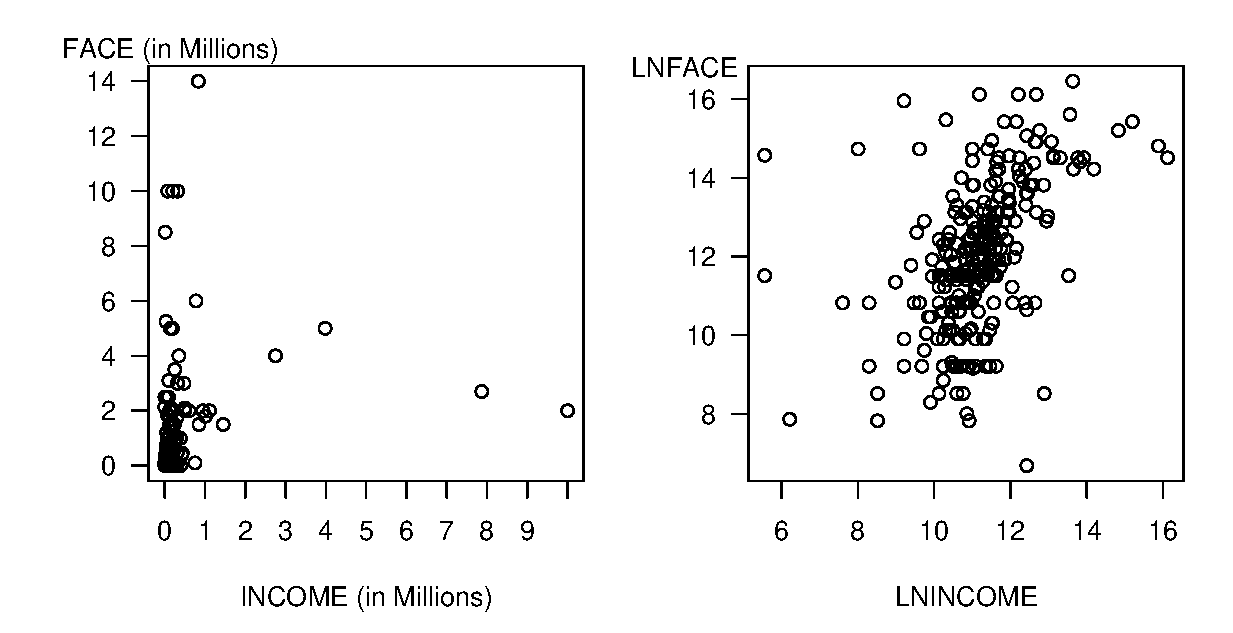
\includegraphics[width=.8\textwidth]{Chapter3/F3TermLifeTwoPlots.eps}
    \caption{\label{F3:TermLifeTwoPlots} \small  Income versus Face Amount of Term Life Insurance. The
left-panel is a plot of face versus income, showing a highly
nonlinear pattern. In the right-hand panel, face versus income is in
natural logarithmic units, suggesting a linear (although variable)
pattern.}
  \end{center}
\end{figure}

The Term Life data are \emph{multivariate} in the sense that several
measurements are taken on each household. It is difficult to produce
a graph of observations in three or more dimensions on a
two-dimensional platform, such as a piece of paper, that is not
confusing, misleading or both. To summarize graphically multivariate
data in regression applications, consider using a \emph{scatterplot
matrix} such as in Figure \ref{F3:TermLifeSMatrix}. Each square of
this figure represents a simple plot of one variable versus another.
For each square, the row variable gives the units of the vertical
axis and the column variable gives the units of the horizontal axis.
The matrix is sometimes called a \emph{half scatterplot matrix}
because only the lower left-hand elements are presented.

\begin{figure}[htp]
  \begin{center}
    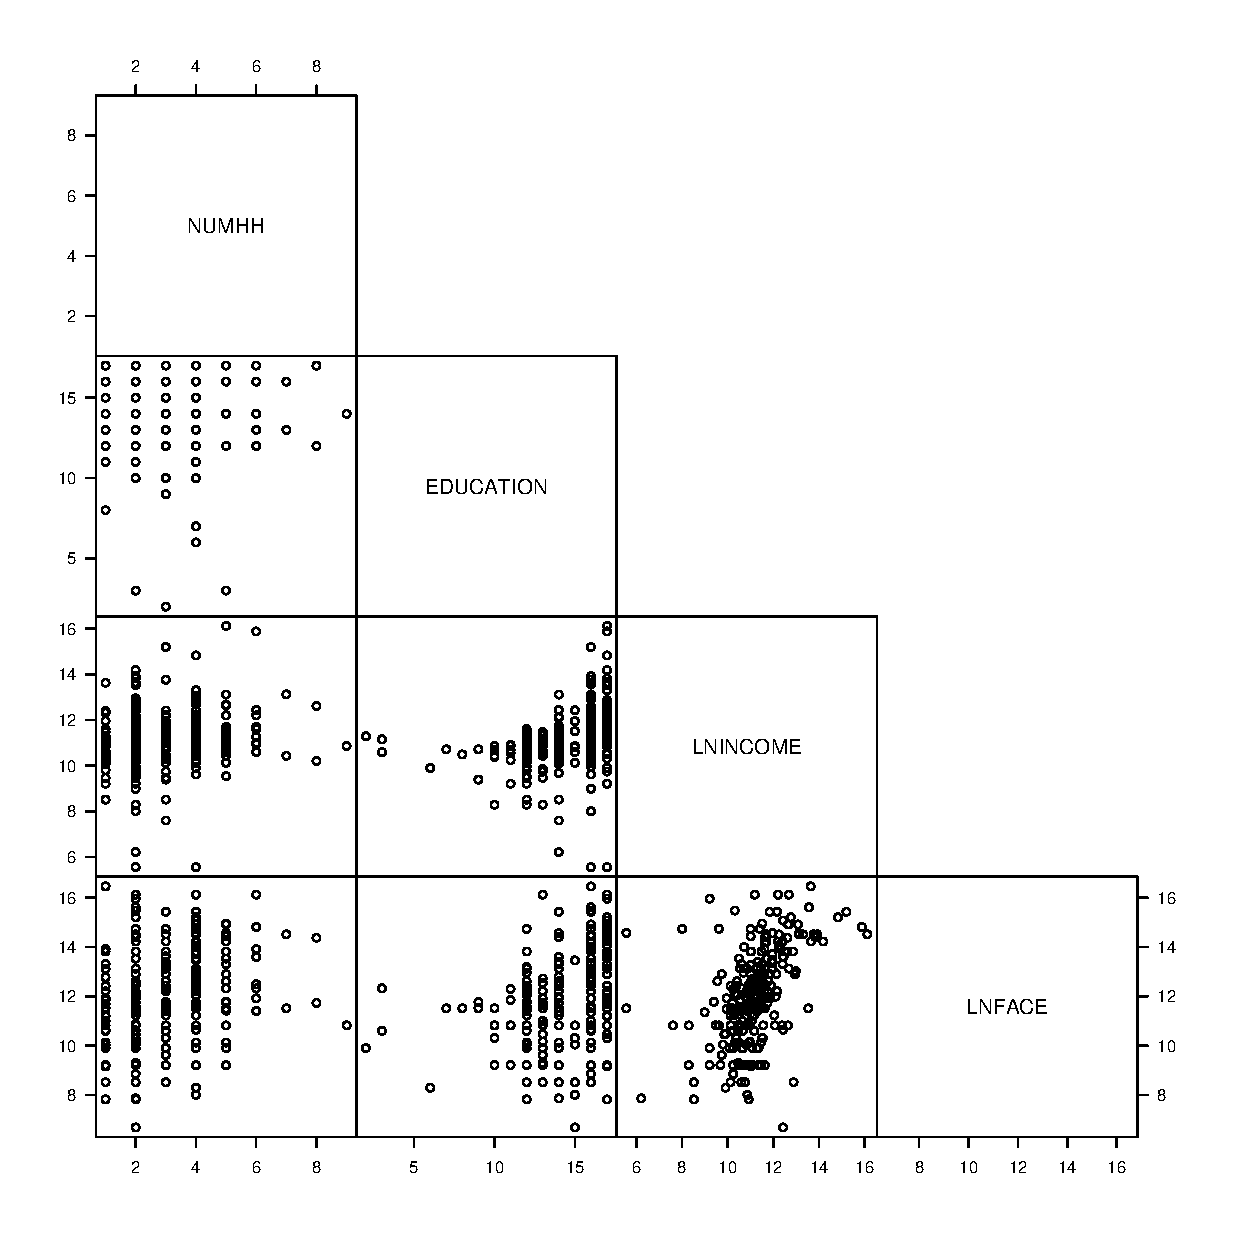
\includegraphics[width=1\textwidth]{Chapter3/F3TermLifeSMatrix.eps}
    \caption{\label{F3:TermLifeSMatrix} \small  Scatterplot
matrix of four variables. Each square is a scatter plot.}
  \end{center}
\end{figure}\index{plots!scatterplot matrix}\index{plots!half scatterplot matrix}

The scatterplot matrix can be numerically summarized using a
correlation matrix. Each correlation in Table \ref{T3:Corr}
corresponds to a square of the scatterplot matrix in Figure
\ref{F3:TermLifeSMatrix}. Analysts often present tables of
correlations because they are easy to interpret. However, remember
that a correlation coefficient merely measures the extent of linear
relationships. Thus, a table of correlations provides a sense of
linear relationships but may miss a nonlinear relationship that can
be revealed in a scatterplot matrix.




\begin{table}[h]
\caption{\label{T3:Corr} Term Life Correlations}
\begin{tabular}{lccc}
\hline
          &  NUMHH    & EDUCATION & LNINCOME  \\
EDUCATION & -0.064~   \\
LNINCOME  & 0.179     & 0.343   \\
LNFACE    & 0.288     & 0.383   & 0.482     \\

\hline
\end{tabular}\end{table}

The scatterplot matrix and corresponding correlation matrix are
useful devices for summarizing multivariate data. They are easy to
produce and to interpret. Still, each device captures only
relationships between pairs of variables and cannot quantify
relationships among several variables.

\subsubsection*{Method of Least Squares}

Consider the question: ``Can knowledge of education, household size
and income help us understand the demand for insurance?'' The
correlations in Table \ref{T3:Corr} and the graphs in Figures
\ref{F3:TermLifeTwoPlots} and \ref{F3:TermLifeSMatrix} suggest that
each variable, EDUCATION, NUMHH and LNINCOME, may be a useful
explanatory variable of LNFACE when taken individually. It seems
reasonable to investigate the \emph{joint} effect of these variables
on a response.

The geometric concept of a \emph{plane} is used to explore the
linear relationship between a response and several explanatory
variables. Recall that a plane extends the concept of a line to more
than two dimensions. A plane may be defined through an algebraic
equation such as
\begin{equation*}
y = b_0 + b_1 x_1 + \ldots + b_k x_k.
\end{equation*}
This equation defines a plane in $k+1$ dimensions. Figure
\ref{F3:3DPlane} shows a plane in three dimensions. For this figure,
there is one response variable, LNFACE, and two explanatory
variables, EDUCATION and LNINCOME (NUMHH is held fixed). It is
difficult to graph more than three dimensions in a meaningful way.

\begin{figure}[htp]
  \begin{center}
    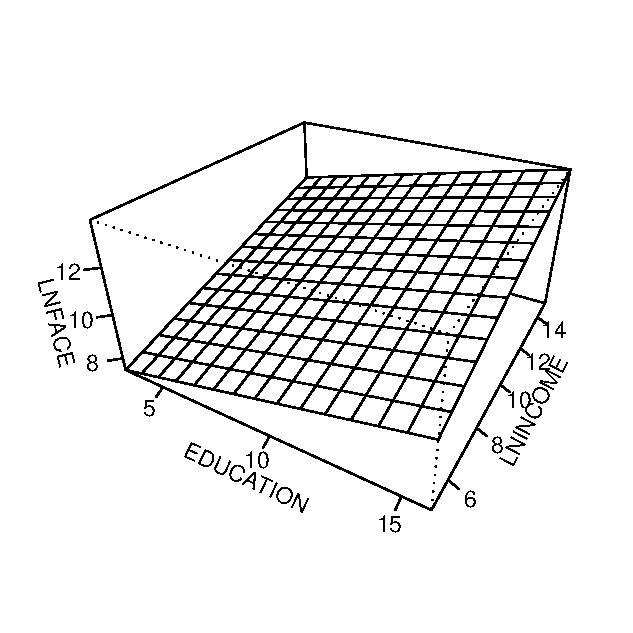
\includegraphics[width=.5\textwidth]{Chapter3/F33DPlane.eps}
    \caption{\label{F3:3DPlane} \small  An example of a three-dimensional plane.}
  \end{center}
\end{figure}

We need a way to determine a plane based on the data. The difficulty
is that in most regression analysis applications, the number of
observations, $n$, far exceeds the number of observations required
to fit a plane, $k+1$. Thus, it is generally not possible to find a
single plane that passes through all $n$ observations. As in Chapter
2, we use the \emph{method of least squares} to determine a plane
from the data.

The method of least squares is based on determining the values of $
b_0^{\ast},b_1^{\ast},\ldots,b_k^{\ast}$ that minimize the quantity
\begin{equation}\label{E3:SSBasic}
SS(b_0^{\ast},b_1^{\ast},\ldots,b_k^{\ast})=\sum_{i=1}^{n}\left(
y_i-\left(
b_0^{\ast}+b_1^{\ast}x_{i1}+\ldots+b_k^{\ast}x_{ik}\right) \right)
^2.
\end{equation}
We drop the asterisk, or star, notation and use $b_0, b_1, \ldots,
b_k$ to denote the best values, known as the \emph{least squares
estimates}. With the least squares estimates, define the \emph{least
squares, or fitted, regression plane} as
\begin{equation*}
\widehat{y} = b_0 + b_1 x_1 + \ldots + b_k x_k.
\end{equation*}\index{least
squares!regression plane}\index{symbols!$b_0, b_1, \ldots, b_k$,
least squares regression coefficients}

The least squares estimates are determined by minimizing
$SS(b_0^{\ast},b_1^{\ast},\ldots,b_k^{\ast})$. It is difficult to
write down the resulting least squares estimators using a simple
formula unless one resorts to matrix notation. Because of their
importance in applied statistical models, an explicit formula for
the estimators is provided below. However, these formulas have been
programmed into a wide variety of statistical and spreadsheet
software packages. The fact that these packages are readily
available allows data analysts to concentrate on the ideas of the
estimation procedure instead of focusing on the details of the
calculation procedures.

As an example, a regression plane was fit to the Term Life data
where three explanatory variables, $x_1$ for EDUCATION, $x_2$ for
NUMHH and $x_3$ for LNINCOME, were used. The resulting fitted
regression plane is

\begin{equation}\label{E3:TermRegression}
\widehat{y} = 2.584 + 0.206 x_1 + 0.306 x_2 + 0.494 x_3.
\end{equation}


\subsubsection*{Matrix Notation}\index{symbols!$\mathbf{y}$, vector of dependent
variables}\index{symbols!$\mathbf{X}$, matrix of explanatory
variables}

Assume that the data are of the form
$(x_{i0},x_{i1},\ldots,x_{ik},y_i)$, where $i = 1, \ldots, n$. Here,
the variable $x_{i0}$ is associated with the ``intercept'' term. That
is, in most applications, we assume that $x_{i0}$ is identically
equal to 1 and thus need not be explicitly represented. However,
there are important applications where this is not the case and
thus, to express the model in general notation, it is included here.
The data are represented in matrix notation using


\begin{equation*}
\mathbf{y}=\left(
\begin{array}{l}
y_1 \\
y_2 \\
\multicolumn{1}{c}{\vdots} \\
y_n%
\end{array}%
\right) ~~~\mathrm{and}~~~\mathbf{X}=\left(
\begin{array}{cccc}
x_{10} & x_{11} & \cdots & x_{1k} \\
x_{20} & x_{21} & \cdots & x_{2k} \\
\vdots & \vdots & \ddots & \vdots \\
x_{n0} & x_{n1} & \cdots & x_{nk}%
\end{array}%
\right) .
\end{equation*}%
Here, \textbf{y} is the $n\times 1$ vector of responses and
\textbf{X} is the $n\times (k+1)$ matrix of explanatory variables.
We use the matrix algebra convention that lower and upper case bold
letters represent vectors and matrices, respectively. (If you need
to brush up on matrices, review Section 2.11.)

\linejed

\textbf{Example: Term Life Insurance - Continued.} Recall that $y$
represents the logarithmic face, $x_1$ for years of education, $x_2$
for number of household members and $x_3$ for logarithmic income.
Thus, there are $k=3$ explanatory variables and $n=275$ households.
The vector of responses and the matrix of explanatory variables are:

\scalefont{0.80}
\begin{equation*}
\mathbf{y}=\left(
\begin{array}{l}
y_1 \\
y_2 \\
\multicolumn{1}{c}{\vdots} \\
y_{275}%
\end{array}%
\right) =\left(
\begin{array}{c}
9.904 \\
11.775 \\
\vdots \\
9.210
\end{array}%
\right) ~~~\mathrm{and}~~~\mathbf{X}=\left(
\begin{array}{cccc}
1 & x_{11} & x_{12} & x_{13} \\
1 & x_{21} & x_{22} & x_{23}\\
\vdots & \vdots & \vdots &\vdots\\
1 & x_{275,1} & x_{275,2} & x_{275,3}%
\end{array}%
\right) =\left(
\begin{array}{cccc}
1 & 16 & 3  & 10.669\\
1 & 9 & 3 & 9.393\\
\vdots & \vdots & \vdots &\vdots\\
1 & 12 & 1 & 10.545%
\end{array}%
\right) .
\end{equation*}
\scalefont{1.25}


\noindent For example, for the first observation in the data set,
the dependent variable is $y_1$=9.904 (corresponding to
$\textrm{exp}(9.904)= \$ 20,000$), for a survey respondent with 16
years of education living in a household with 3 people with
logarithmic income of 10.669 ($\exp (10.669)= \$ 43,000)$.

\linejed

Under the least squares estimation principle, our goal is to choose
the coefficients $b_0^{\ast},b_1^{\ast},\ldots,b_k^{\ast}$ to
minimize the sum of squares function
$SS(b_0^{\ast},b_1^{\ast},\ldots,b_k^{\ast})$. Using calculus, we
return to equation (\ref{E3:SSBasic}), take partial derivatives with
respect to each coefficient and set these quantities equal to zero:
\begin{equation*}
\frac{\partial }{\partial
b_j^{\ast}}SS(b_0^{\ast},b_1^{\ast},\ldots,b_k^{\ast})=\sum_{i=1}^{n}\left(
-2x_{ij}\right) \left( y_i-\left(
b_0^{\ast}+b_1^{\ast}x_{i1}+\ldots+b_k^{\ast}x_{ik}\right) \right)
=0,~~~\mathrm{for}~~j=0,1,\ldots .,k.
\end{equation*}
This is a system of $k+1$ equations and $k+1$ unknowns that can be readily
solved using matrix notation, as follows.

We may express the vector of parameters to be minimized as
$\mathbf{b}^{\ast}=(b_0^{\ast},b_1^{\ast},\ldots,b_k^{\ast})^{\prime}$.
Using this,
the sum of squares can be written as $SS(\mathbf{b}^{\ast})=(\mathbf{y-Xb}%
^{\ast})^{\prime}(\mathbf{y-Xb}^{\ast}).$ Thus, in matrix form, the
solution to the minimization problem can be expressed as $(\partial
/\partial \mathbf{b}^{\ast})SS(\mathbf{b}^{\ast})=\mathbf{0}$. This
solution satisfies the \emph{normal equations}
\begin{equation}\label{E3:NormalEquations}
\mathbf{X^{\prime}Xb}=\mathbf{X}^{\prime}\mathbf{y}.
\end{equation}
Here, the asterisk notation (*) has been dropped to denote the fact that $%
\mathbf{b}=(b_0,b_1,\ldots,b_k)^{\prime}$ represents the best vector
of values in the
sense of minimizing $SS(\mathbf{b}^{\ast})$ over all choices of $\mathbf{b}%
^{\ast}$.\index{symbols!$\mathbf{b}$, vector of regression
coefficients}\index{normal equations}

The least squares estimator $\mathbf{b}$ need not be unique.
However, assuming that the explanatory variables are not linear
combinations of one another, we have that $\mathbf{X^{\prime}X}$ is
invertible. In this case, we can write the unique solution as
\begin{equation}\label{E3:LSEstimates}
\mathbf{b}=\left( \mathbf{X^{\prime}X}\right) ^{-1}\mathbf{X}^{\prime}%
\mathbf{y}.
\end{equation}

\noindent To illustrate, for the Term Life example, equation
(\ref{E3:TermRegression}) yields
\begin{equation*}
\mathbf{b} = \left(
\begin{array}{c}
b_0 \\ b_1 \\ b_2 \\ b_3 \\
\end{array}
\right) = \left(
\begin{array}{c}
2.584 \\ 0.206 \\ 0.306 \\ 0.494 \\
\end{array}
\right).
\end{equation*}

\section{Linear Regression Model and Properties of Estimators}

In the previous section, we learned how to use the method of least
squares to fit a regression plane with a data set. This section
describes the assumptions underpinning the regression model and some
of the resulting properties of the regression coefficient
estimators. With the model and the fitted data, we will be able to
draw inferences about the sample data set to a larger population.
Moreover, we will later use these regression model assumptions to
help us improve the model specification in Chapter 5.

\subsection{Regression Function}

Most of the assumptions of the multiple linear regression model will
carry over directly from the basic linear regression model
assumptions introduced in Section 2.2. The primary difference is
that we now summarize the relationship between the response and the
explanatory variables through the \emph{regression
function}\index{regression function}

\begin{equation}\label{E3:MLRegressionFct}
\mathrm{E~}y=\beta_0 x_0+\beta_1 x_1+\ldots+\beta_k x_k,
\end{equation}%
that is linear in the parameters $\beta_0,\ldots ,\beta_k$.
Henceforth, we will use $x_0=1$ for the variable associated with the
parameter $\beta_0;$ this is the default in most statistical
packages and most applications of regression include the intercept
term $\beta_0$. The intercept is the expected value of $y$ when all
of the explanatory variables are equal to zero. Although rarely of
interest, the term $\beta_0$ serves to set the height of the fitted
regression plane.

\marginparjed{Interpret $\beta_j$ to be the expected change in $y$
per unit change in $x_j$ assuming all other explanatory variables
are held fixed.}\index{symbols!$\beta_j$, regression coefficient
associated with $x_j$}

In contrast, the other betas are typically important parameters from
a regression study. To help interpret them, we initially assume that
$x_j$ varies continuously and is not related to the other
explanatory variables. Then, we can interpret $\beta_j$ as the
expected change in $y$ per unit change in $x_j$ \emph{assuming all
other explanatory variables are held fixed}. That is, from calculus,
you will recognize that $\beta_j$ can be interpreted as a partial
derivative. Specifically, using equation (\ref{E3:MLRegressionFct}),
we have that
\begin{equation*}
\beta_j=\frac{\partial }{\partial x_j}\mathrm{E}~y.
\end{equation*}


\subsection{Regression Coefficient
Interpretation}\index{transformations!logarithmic}

Let us examine the regression coefficient estimates from the Term
Life Insurance example and focus initially on the \emph{sign} of the
coefficients. For example, from equation (\ref{E3:TermRegression}),
the coefficient associated with NUMHH is $b_2 = 0.306>0$. If we
consider two households that have the same income and the same level
of education, then the larger household (in terms of NUMHH) is
expected to demand \textit{more} term life insurance under the
regression model. This is a sensible interpretation, larger
households have more dependents for which term life insurance can
provide needed financial assets in the event of the untimely death
of a breadwinner. The positive coefficient associated with income
($b_3 = 0.494$) is also plausible; households with larger incomes
have more disposable dollars to purchase insurance. The positive
sign associated with EDUCATION ($b_1 = 0.206)$ is also reasonable,
more education suggests that respondents are more aware of their
insurance needs, other things being equal.

You will also need to interpret the \emph{amount} of the regression
coefficient. Consider first the EDUCATION coefficient. Using
equation (\ref{E3:TermRegression}), fitted values of
$\widehat{LNFACE}$ were calculated by allowing EDUCATION to vary and
keeping NUMHH and LNINCOME fixed at the sample averages. The results
are:
\begin{center}
\scalefont{0.9}
\begin{tabular}{lrrrr}
\hline \multicolumn{5}{c}{\textit{Effects of Small Changes in Education}} \\
\hline
 EDUCATION                &         14 &       14.1 &       14.2 &       14.3 \\
 $\widehat{LNFACE}$       &     11.883 &     11.904 &     11.924 &     11.945 \\
   $\widehat{FACE}$       &    144,803 &    147,817 &    150,893 &    154,034 \\
$\widehat{FACE}$ \% Change&            &      2.081 &      2.081 &      2.081 \\
\hline
\end{tabular}
\scalefont{1.1111}
\end{center}

\noindent As EDUCATION increases,  $\widehat{LNFACE}$ increases.
Further, the amount of $\widehat{LNFACE}$ increase is a constant
0.0206. This comes directly from equation (\ref{E3:TermRegression});
as EDUCATION increases by 0.1 years, we expect the demand for
insurance to increase by 0.0206 logarithmic dollars, holding NUMHH
and LNINCOME fixed. This interpretation is correct but most product
development directors are not overly fond of logarithmic dollars. To
return to dollars, fitted face values can be calculated through
exponentiation as $ \widehat{FACE}=\textrm{exp}(\widehat{LNFACE})$.
Moreover, the percentage change can be computed; for example,
$100*(147,817/144,803 - 1) \approx 2.08\% $. This provides another
interpretation of the regression coefficient; as EDUCATION increases
by 0.1 years, we expect the demand for insurance to increase by
2.08\%. This is a simple consequence of calculus using $ \partial
\textrm{ln} ~y /
\partial x  = \left(\partial y / \partial x \right) / y$; that is, a
small change in the logarithmic value of $y$ equals a small change
in $y$ as a proportion of $y$. It is because of this calculus result
that we use natural logs instead of common logs in regression
analysis. Because this table uses a discrete change in EDUCATION,
the 2.08\% differs slightly from the continuous result $0.206 \times
(\mathrm{change~in~EDUCATION}) = 2.06\%$. However, this proximity is
usually regarded as suitable for interpretation purposes.

Continuing this logic, consider small changes in logarithmic income.

\begin{center}
\scalefont{0.9}
\begin{tabular}{lrrrr}
\hline \multicolumn{5}{c}{\textit{Effects of Small Changes in Logarithmic Income}} \\
 \hline
  LNINCOME &         11 &       11.1 &       11.2 &       11.3 \\
    INCOME &     59,874 &     66,171 &     73,130 &     80,822 \\
INCOME \% Change  &            &      10.52 &      10.52 &      10.52 \\
\hline
 $\widehat{LNFACE}$ &     11.957 &     12.006 &     12.055 &     12.105 \\
 $\widehat{FACE}$ &    155,831 &    163,722 &    172,013 &    180,724  \\
$\widehat{FACE}$ \% Change &            &       5.06 &       5.06 &       5.06 \\
\hline
$\widehat{FACE}$ \% Change / INCOME \% Change &            &       0.482 &      0.482 &      0.482 \\
\hline
\end{tabular}
\scalefont{1.1111}
\end{center}

\index{actuarial \& financial terms and concepts!elasticity}


\noindent We can use the same logic to interpret the LNINCOME
coefficient in equation (\ref{E3:TermRegression}). As logarithmic
income increases by 0.1 units, we expect the demand for insurance to
increase by 5.06\%. This takes care of logarithmic units in the $y$
but not the $x$. We can use the same logic to say that as
logarithmic income increases by 0.1 units, INCOME increases by
10.52\%. Thus, a 10.52\% change in INCOME corresponds to a 5.06\%
change in FACE. Summarizing, we say that, holding NUMHH and
EDUCATION fixed, we expect that a 1\% increase in INCOME is
associated with a 0.482\% increase in $\widehat{FACE}$ (as before,
this is close to the parameter estimate $b_3 = 0.494$). The
coefficient associated with income is known as an \emph{elasticity}
in economics. In economics, elasticity is the ratio of the percent
change in one variable to the percent change in another variable.
Mathematically, we summarize this as
\begin{equation*}
\frac{\partial \textrm{ln} ~y}{\partial \textrm{ln} ~x} =
\left(\frac{\partial ~y}{y}\right)/\left(\frac{\partial
~x}{x}\right).
\end{equation*}

\subsection{Model Assumptions}\index{model assumptions!observables
representation}\index{model assumptions!error representation}

As in Section 2.2 for a single explanatory variable, there are two
sets of assumptions that one can use for multiple linear regression.
They are equivalents sets, each having comparative advantages as we
proceed in our study of regression. The ``observables''
representation focuses on variables of interest
$(x_{i1},\ldots,x_{ik},y_i).$ The ``error representation'' provides
a springboard for motivating our goodness of fit measures and study
of residual analysis. However, the latter set of assumptions focuses
on the additive errors case and obscures the sampling basis of the
model.


\scalefont{0.8}

\begin{center}
\begin{tabular}{cc}
\hline
\multicolumn{2}{c}{\large{Multiple Linear Regression Model Sampling Assumptions}} \\
Observables Representation & Error Representation \\ \hline
\multicolumn{1}{l}{F1. $\mathrm{E}~y_i=\beta_0+\beta_1
x_{i1}+\ldots+\beta_k x_{ik}$.} & \multicolumn{1}{l}{E1.
$y_i=\beta_0+\beta_1 x_{i1}+\ldots+\beta_k x_{ik}+\varepsilon_i$.} \\
\multicolumn{1}{l}{F2. $\{x_{i1},\ldots ,x_{ik}\}$} &
\multicolumn{1}{l}{E2.
$\{x_{i1},\ldots ,x_{ik}\}$} \\
are non-stochastic variables. & are non-stochastic variables. \\
\multicolumn{1}{l}{F3. $\mathrm{Var}~y_i=\sigma^2$.} &
\multicolumn{1}{l}{E3. $\mathrm{E}~\varepsilon_i=0$ and $\mathrm{Var}~\varepsilon_i=\sigma^2$.} \\
\multicolumn{1}{l}{F4. \{$y_i$\} are independent random variables.}
& \multicolumn{1}{l}{E4. \{$\varepsilon_i$\} are independent random
variables.} \\
\multicolumn{1}{l}{F5. \{$y_i$\} are normally distributed.} &
\multicolumn{1}{l}{E5. \{$\varepsilon_i$\} are normally distributed.} \\
\hline
\end{tabular}
\end{center}


\scalefont{1.25}

To further motivate Assumptions F2 and F4, we will usually assume
that our data have been realized as the result of a stratified
sampling scheme, where each unique value of
$\{x_{i1},\ldots,x_{ik}\}$ is treated as a stratum. That is, for
each value of $\{x_{i1},\ldots,x_{ik}\}$, we draw a random sample of
responses from a population. Thus, responses within each stratum are
independent from one another, as are responses from different
strata. Chapter 6 will discuss this sampling basis in further
detail.

\subsection{Properties of Regression Coefficient Estimators}
\index{symbols!$\boldsymbol \beta$, vector of regression
coefficients}

Section \ref{S3:LSMethod} described the least squares method for
estimating regression coefficients. With the regression model
assumptions, we can establish some basic properties of these
estimators. To do this, from Section 2.11.4 we have that the
expectation of a vector is the vector of expectations, so that
\begin{equation*}
\mathrm{E}~\mathbf{y}=\left(
\begin{array}{l}
\mathrm{E}~y_1 \\
\mathrm{E}~y_2 \\
\multicolumn{1}{c}{\vdots} \\
\mathrm{E}~y_n
\end{array}
\right) .
\end{equation*}
Further, basic matrix multiplication shows that
\begin{equation*}
\mathbf{X} \boldsymbol \beta=\left(
\begin{array}{cccc}
1 & x_{11} & \cdots & x_{1k} \\
1 & x_{21} & \cdots & x_{2k} \\
\vdots & \vdots & \ddots & \vdots \\
1 & x_{n,1} & \cdots & x_{n,k}%
\end{array}%
\right) \left(
\begin{array}{c}
\beta_0 \\
\beta_1 \\
\vdots \\
\beta_k%
\end{array}
\right) =\left(
\begin{array}{c}
\beta_0 + \beta_1 x_{11} + \cdots + \beta_k x_{1k} \\
\beta_0 + \beta_1 x_{21} + \cdots + \beta_k x_{2k} \\
\vdots \\
\beta_0 + \beta_1 x_{n1} + \cdots + \beta_k x_{nk}
\end{array}
\right) .
\end{equation*}
Because the $i$th row of assumption F1 is $\mathrm{E}~y_i = \beta_0
+ \beta_1 x_{i1} + \cdots + \beta_k x_{ik}$, we may re-write this
assumption in matrix formulation as
$\mathrm{E}~\mathbf{y}=\mathbf{X}\boldsymbol \beta$. We are now in a
position to state the first important property of least squares
regression estimators.

\bigskip

\boxedjed

\textbf{Property 1}. Consider a regression model and let Assumptions
F1-F4 hold. Then, the estimator $\mathbf{b}$ defined in equation
(\ref{E3:LSEstimates}) is an unbiased estimator of the parameter
vector $\boldsymbol \beta$.
\end{boxedminipage}\index{estimator!unbiased}

\bigskip

To establish Property 1, we have that

\begin{equation*}
\mathrm{E}~\mathbf{b} = \mathrm{E}~\left(
(\mathbf{X^{\prime}X)}^{-1}\mathbf{X}^{\prime}\mathbf{y}\right)
=(\mathbf{X^{\prime}X)}^{-1}\mathbf{X}^{\prime}\mathrm{E}~\mathbf{y}
=(\mathbf{X^{\prime}X)}^{-1} \mathbf{X}^{\prime} \left( \mathbf{X}
\boldsymbol \beta \right) = \boldsymbol \beta,
\end{equation*}
using matrix multiplication rules. This chapter assumes that
$\mathbf{X^{\prime}X}$ is invertible. One can also show that the
least squares estimator need only be a solution of the normal
equations for unbiasedness (not requiring that
$\mathbf{X^{\prime}X}$ be invertible, see Section 4.7.3). Thus,
$\mathbf{b}$ is said to be an \emph{unbiased estimator }of
$\boldsymbol \beta$. In particular, E $b_j$ = $\beta_j$ for $j =
0,1,\ldots,k$.

Because independence implies zero covariance, from Assumption F4 we
have that $\mathrm{Cov}(y_i,y_j)=0$ for $i\neq j$. From this,
Assumption F3 and the definition of the variance of a vector, we
have that
\begin{equation*}
\mathrm{Var~}\mathbf{y}=\left(
\begin{array}{cccc}
\mathrm{Var~}y_1 & \mathrm{Cov}(y_1,y_2) & \cdots & \mathrm{Cov}
(y_1,y_n) \\
\mathrm{Cov}(y_2,y_1) & \mathrm{Var~}y_2 & \cdots & \mathrm{Cov}
(y_2,y_n) \\
\vdots & \vdots & \ddots & \vdots \\
\mathrm{Cov}(y_n,y_1) & \mathrm{Cov}(y_n,y_2) & \cdots &
\mathrm{Var~ }y_n
\end{array}
\right) =\left(
\begin{array}{cccc}
\sigma^2 & 0 & \cdots & 0 \\
0 & \sigma^2 & \cdots & 0 \\
\vdots & \vdots & \ddots & \vdots \\
0 & 0 & \cdots & \sigma^2
\end{array}
\right) =\sigma^2\mathbf{I},
\end{equation*}
where $\mathbf{I}$\ is an an $n\times n$ identity matrix. We are now
in a position to state the second important property of least
squares regression estimators.
\bigskip

\boxedjed

\textbf{Property 2.} Consider a regression model and let Assumptions
F1-F4 hold. Then, the estimator $\mathbf{b}$ defined in equation
(\ref{E3:LSEstimates}) has variance $\mathrm{Var~}\mathbf{b}
=\sigma^2(\mathbf{X^{\prime}X)}^{-1}.$
\end{boxedminipage}
\bigskip

To establish Property 2, we have that

\begin{eqnarray*}
\mathrm{Var~}\mathbf{b} &=&\mathrm{Var}\left(
(\mathbf{X^{\prime}X)}^{-1} \mathbf{X}^{\prime}\mathbf{y}\right)
=\left[ (\mathbf{X^{\prime}X)}^{-1} \mathbf{X}^{\prime}\right]
\mathrm{Var}\left( \mathbf{y}\right) \left[
\mathbf{X}(\mathbf{X^{\prime}X)}^{-1}\right] \\
&=&\left[ (\mathbf{X^{\prime}X)}^{-1}\mathbf{X}^{\prime}\right]
\sigma^2 \mathbf{I}\left[
\mathbf{X}(\mathbf{X^{\prime}X)}^{-1}\right] =\sigma^2(
\mathbf{X^{\prime}X)}^{-1}\mathbf{X}^{\prime}\mathbf{X}(\mathbf{X^{\prime}X)}^{-1}=\sigma
^2(\mathbf{X^{\prime}X)}^{-1},
\end{eqnarray*}
as required. This important property will allow us to measure the
precision of the estimator $\mathbf{b}$ when we discuss statistical
inference. Specifically, by the definition of the variance of a
vector (see Section 2.11.4),
\begin{equation}\label{E3:VarVec}
\mathrm{Var~}\mathbf{b}=\left(
\begin{array}{cccc}
\mathrm{Var~}b_0 & \mathrm{Cov}(b_0,b_1) & \cdots & \mathrm{Cov}%
(b_0,b_k) \\
\mathrm{Cov}(b_1,b_0) & \mathrm{Var~}b_1 & \cdots & \mathrm{Cov}%
(b_1,b_k) \\
\vdots & \vdots & \ddots & \vdots \\
\mathrm{Cov}(b_k,b_0) & \mathrm{Cov}(b_k,b_1) & \cdots & \mathrm{Var~%
}b_k%
\end{array}
\right) =\sigma^2 (\mathbf{X^{\prime}X)}^{-1}.
\end{equation}
Thus, for example, $\mathrm{Var~}b_j$ is $\sigma^2$ times the
$(j+1)st$
diagonal entry of $(\mathbf{X^{\prime}X)}^{-1}$. As another example, $\mathrm{Cov}%
(b_0,b_j)$ is $\sigma^2$ times the element in the first row and $%
(j+1)st$ column of $(\mathbf{X^{\prime}X)}^{-1}$.

Although alternative methods are available that are preferable for
specific applications, the least squares estimators have proven to
be effective for many routine data analyses. One desirable
characteristic of least squares regression estimators is summarized
in the following well-known result.

\bigskip
\boxedjed\index{theorems!Gauss-Markov}

\textbf{Gauss-Markov Theorem.} Consider the regression model and let
Assumptions F1-F4 hold. Then, within the class of estimators that
are linear functions of the responses, the least squares estimator
$\mathbf{b}$ defined in equation (\ref{E3:LSEstimates}) is the
minimum variance unbiased estimator of the parameter vector
$\boldsymbol \beta$.
\end{boxedminipage}
\bigskip

\marginparjed{The Gauss-Markov theorem states that the least squares
estimator is the most precise in the sense that it has the smallest
variance.}

We have already seen in Property 1 that the least squares estimators
are unbiased. The Gauss-Markov theorem states that the least squares
estimator is the most precise in the sense that it has the smallest
variance. (In a matrix context, ``minimum variance'' means that if
$\mathbf{b}^{\ast}$ is any other estimator, then the difference of
the variance matrices, $\mathrm{Var~}
\mathbf{b}^{\ast}\mathbf{-}\mathrm{Var~}\mathbf{b}$, is nonnegative
definite.)

An additional important property concerns the distribution of the
least squares regression estimators.

\bigskip
\boxedjed

\textbf{Property 3}. Consider a regression model and let Assumptions
F1-F5 hold. Then, the least squares estimator $\mathbf{b}$ defined
in equation (\ref{E3:LSEstimates}) is normally distributed.
\end{boxedminipage}
\bigskip

\noindent To establish Property 3, we define the weight vectors,
$\mathbf{w}_i=(\mathbf{X^{\prime}X)}^{-1}\left( 1,x_{i1}, \ldots,
x_{ik}\right) ^{\prime}$. With this notation, we note that
\begin{equation*}
\mathbf{b=}(\mathbf{X^{\prime}X)}^{-1}\mathbf{X}^{\prime}\mathbf{y=}
\sum_{i=1}^{n}\mathbf{w}_iy_i,
\end{equation*}
so that $\mathbf{b}$ is a linear combination of responses. With
Assumption F5, the responses are normally distributed. Because
linear combinations of normally distributed random variables are
normally distributed, we have the conclusion of Property 3. This
result underpins much of the statistical inference that will be
presented in Sections 3.4 and 4.2.


\section{Estimation and Goodness of Fit}\index{goodness of fit
statistics}

\subsubsection*{Residual Standard Deviation}

Additional properties of the regression coefficient estimators will
be discussed when we focus on statistical inference. We now continue
our estimation discussion by providing an estimator of the other
parameter in the linear regression model, $\sigma^2$.

Our estimator for $\sigma^2$ can be developed using the principle of
replacing theoretical expectations by sample averages. Examining
$\sigma^2=\mathrm{E}\left( y-\mathrm{E~}y\right)^2$, replacing the
outer expectation by a sample average suggests using the estimator $
n^{-1}\sum_{i=1}^{n}(y_i-\mathrm{E~}y_i)^2$. Because we do not
observe $\mathrm{E}~y_i = \beta_0 + \beta_1 x_{i1} + \cdots +
\beta_k x_{ik}$, we use in its place the corresponding observed
quantity $b_0 + b_1 x_{i1}+\ldots+b_k x_{ik}=\widehat{y}_i$. This
leads to the following.


\bigskip

\boxedjed

\textit{Definition}. An estimator of $\sigma^2$, the \emph{mean
square error (MSE)}, is defined as
\begin{equation} \label{E3:s2}
s^2=\frac{1}{n-(k+1)}\sum_{i=1}^{n}\left( y_i-\widehat{y}_i\right)
^2.
\end{equation}
The positive square root, $s=\sqrt{s^2},$ is called the
\emph{residual standard deviation}.

\end{boxedminipage}
\bigskip


This expression generalizes the definition in equation (2.3), which
is valid for $k=1$. It turns out, by using $n-(k+1)$ instead of $n$
in the denominator of equation (\ref{E3:s2}), that $s^2$ is an
unbiased estimator of $\sigma^2$. Essentially, by using
$\widehat{y}_i$\ instead of $\mathrm{E~}y_i$ in the definition, we
have introduced some small dependencies among the deviations from
the responses $y_i-\widehat{y}_i$, thus reducing the overall
variability. To compensate for this lower variability, we also
reduce the denominator in the definition of $s^2$.

To provide further intuition on the choice of $n-(k+1)$ in the
definition of $s^2$, we introduced the concept of residuals in the
context of multiple linear regression. From Assumption E1 recall
that the random errors can be expressed as $\varepsilon
_i=y_i-(\beta_0 + \beta_1 x_{i1}+\cdots + \beta_k x_{ik}).$ Because
the parameters $\beta_0,\ldots,\beta_k$ are not observed, the errors
themselves are not observed. Instead, we examine the ``estimated
errors,'' or \emph{residuals}, defined by $e_i = y_i-\widehat{y}_i.$

Unlike errors, there exist certain dependencies among the residuals. One
dependency is due to the algebraic fact that the average residual is zero.
Further, there must be at least $k+2$ observations for there to be variation
in the fit of the plane. If we have only $k+1$ observations, we could fit a
plane to the data perfectly, resulting in no variation in the fit. For
example, if $k=1$, because two observations determine a line, then at least
three observations are required to observe any deviation from the line.
Because of these dependencies, we have only $n-(k+1)$ free, or unrestricted,
residuals to estimate the variability about the regression plane.

The positive square root of $s^2$ is our estimator of $\sigma $.
Using
residuals, it can be expressed as%
\begin{equation}\label{E3:ResidStddev}
s=\sqrt{\frac{1}{n-(k+1)}\sum_{i=1}^{n}e_i^2.}
\end{equation}%
Because it is based on residuals, we refer to $s$ as the
\emph{residual standard deviation}. The quantity $s$ is a measure of
our ``typical error.'' For this reason, $s$ is also called the
\emph{standard error of the estimate}.

\subsubsection*{The Coefficient of Determination: $R^2$}

To summarize the goodness of fit of the model, as in Chapter 2 we
partition the variability into pieces that are ``explained'' and
``unexplained'' by the regression fit. Algebraically, the
calculations for regression using many variables are similar to the
case of using only one variable. Unfortunately, when dealing with
many variables, we do lose the easy graphical interpretation such as
in Figure 2.4.

\index{symbols!$Total~SS$, total sum of squares}

Begin with the total sum of squared deviations, $Total~SS=\sum_{i=1}^{n}%
\left( y_i-\overline{y}\right)^2$, as our measure of the total
variation in the data set. As in equation (2.1), we may then
interpret the equation
\begin{equation*}
\begin{tabular}{ccccc}
$\underbrace{y_i-\overline{y}}$ & = &
$\underbrace{y_i-\widehat{y}_i}$
& + & $\underbrace{\widehat{y}_i-\overline{y}}$ \\
{\small total} & {\small =} & {\small unexplained} & {\small +} & {\small %
explained} \\
{\small deviation} &  & {\small deviation} &  & {\small deviation}%
\end{tabular}%
\end{equation*}%
as the ``deviation without knowledge of the explanatory variables
equals the deviation not explained by the explanatory variables plus
deviation explained by the explanatory variables.'' Squaring each
side and summing over all observations yields
\begin{equation*}
Total~SS = Error~SS + Regression~SS
\end{equation*}%
where $Error~SS=\sum_{i=1}^{n}\left( y_i-\widehat{y}_i\right)^2$\
and \ $Regression~SS = \sum_{i=1}^{n}\left(
\widehat{y}_i-\overline{y}\right)^2$. As in Section 2.3 for the one
explanatory variable case, the sum of the cross-product terms turns
out to be zero.

A statistic that summarizes this relationship is the
\emph{coefficient of determination},
\begin{equation*}
R^2=\frac{Regression~SS}{Total~SS}.
\end{equation*}
We interpret $R^2$ to be the proportion of variability explained by
the regression function.

If the model is a desirable one for the data, one would expect a
strong relationship between the observed responses and those
``expected'' under the model, the fitted values. An interesting
algebraic fact is the following. If one squares the correlation
coefficient between the responses and the fitted values, we get the
coefficient of determination, that is,
\begin{equation*}
R^2=\left[ r \left(y,\widehat{y} \right) \right]^2.
\end{equation*}
As a result, $R$, the positive square root of $R^2$, is called the
\emph{multiple correlation coefficient}. It can be interpreted as
the correlation between the response and the best linear combination
of the explanatory variables, the fitted values. (This relationship
is developed using matrix algebra in the technical supplement
Section 5.10.1.)

\index{goodness of fit statistics!coefficient of determination,
$R^2$}\index{symbols!$R^2$, coefficient of determination}
\index{goodness of fit statistics!multiple correlation coefficient,
$R$}\index{symbols!$R$, multiple correlation
coefficient}\index{correlation coefficients!multiple}

The variability decomposition is also summarized using the
\emph{analysis of variance}, or \emph{ANOVA}, table, as
follows.\index{analysis of variance, ANOVA, table}

\scalefont{0.9}

\begin{center}
\begin{tabular}{l|lcl}
\hline
\multicolumn{4}{c}{ANOVA\ Table} \\ \hline
Source & Sum of Squares & $df$ & Mean Square \\ \hline
Regression & $Regression~SS$ & $k$ & $Regression~MS$ \\
Error & $Error~SS$ & $n-(k+1)$ & $MSE$ \\
Total & $Total~SS$ & $n-1$ &  \\ \hline
\end{tabular}
\end{center}
\scalefont{1.1111}

\index{symbols!$Error~MS$, error mean square}\index{symbols!$MSE$,
error mean square}\index{symbols!$Regrssion~MS$, regression mean
square}\index{symbols!$Regression~SS$, regression sum of
squares}\index{symbols!$Error~SS$, error sum of squares}

\noindent The mean square column figures are defined to be the sum
of squares figures divided by their respective degrees of freedom.
The error degrees of freedom denotes the number of unrestricted
residuals. It is this number that we use in our definition of the
``average,'' or mean, square error. That is, we define
\begin{equation*}
MSE=Error~MS=\frac{Error~SS}{n-(k+1)}=s^2.
\end{equation*}
Similarly, the regression degrees of freedom is the number of
explanatory variables. This yields
\begin{equation*}
Regression~MS=\frac{Regression~SS}{k}.
\end{equation*}
When discussing the coefficient of determination, it can be
established that whenever an explanatory variable is added to the
model, $R^2$ never decreases. This is true whether or not the
additional variable is useful. We would like a measure of fit that
decreases when useless variables are entered into the model as
explanatory variables. To circumvent this anomaly, a widely used
statistic is the \emph{coefficient of determination adjusted for
degrees of freedom}, defined by
\begin{equation}\label{E3:AdjustedR2}
R_{a}^2=1-\frac{(Error~SS)/[n-(k+1)]}{(Total~SS)/(n-1)}=1-\frac{s^2}{%
s_{y}^2}.
\end{equation}
To interpret this statistic, note that $s_y^2$ does not depend on
the model nor the model variables. Thus, $s^2$ and $R_a^2$ are
equivalent measures of model fit. As the model fit improves, then
$R_{a}^2$ becomes larger and $s^2$ becomes smaller, and vice versa.
Put another way, choosing a model with the smallest $s^2$ is
equivalent to choosing a model with the largest $R_a^2$.

\index{goodness of fit statistics!coefficient of determination
adjusted for degrees of freedom, $R_a^2$}\index{symbols!$R_a^2$,
coefficient of determination adjusted for degrees of freedom}

\linejed

\textbf{Example: Term Life Insurance - Continued.} To illustrate,
Table \ref{T3:ANOVATerm} displays the summary statistics for the
regression of LNFACE on EDUCATION, NUMHH and LNINCOME. From the
degrees of freedom column, we remind ourselves that there are three
explanatory variables and 275 observations. As measures of model
fit, the coefficient of determination is $ R^2=34.3\%$
(=328.47/958.90) and the residual standard deviation is $s=1.525$
($=\sqrt{2.326}$ ). If we were to attempt to estimate the
logarithmic face amount without knowledge of the explanatory
variables EDUCATION, NUMHH and LNINCOME, then the size of the
typical error would be $s_y=1.871$ ($=\sqrt{958.90/274}$). Thus, by
taking advantage of our knowledge of the explanatory variables, we
have been able to reduce the size of the typical error. The measure
of model fit that compares these two estimates of variability is the
adjusted coefficient of determination, $ R_a^2=1 - 2.326/1.871^2 =
33.6\%.$


\begin{table}[h]
\scalefont{0.9} \caption{\label{T3:ANOVATerm} Term Life ANOVA Table}
\begin{tabular}{lrrr}
 \hline Source
& Sum of Squares & $df$ & Mean Square \\ \hline

Regression & 328.47 & 3 & 109.49 \\
Error      & 630.43 & 271 &  2.326 \\
Total & 958.90 & 274 &   \\ \hline
\end{tabular}
\linetjed \scalefont{1.1111}
\end{table}



\newpage

\linejed

\textbf{Example: Why do Females Live Longer than
Males?}\ecaptionjed{Why do Females Live Longer than Males?} In an
article with this title, Lemaire (2002) examined what he called the
``female advantage,'' the difference in life expectancy between
females and males. Life expectancies are of interest because they
are widely used measures of a nation's health. Lemaire examined data
from $n=169$ countries and found that the average female advantage
was 4.51 years worldwide. He sought to explain this difference based
on 45 behaviorial measures, variables that capture a nation's degree
of economic modernization, social/cultural/religious mores,
geographic position and quality of health care available.

After a detailed analysis, Lemaire reports coefficients from a
regression model that appear in Table \ref{T6:FemaleAdvantage}. This
regression model explains $R^2 = 61\%$ of the variability. It is a
parsimonious model consisting of only $k=4$ of the original 45
variables.

\scalefont{0.9}  \begin{center}  \begin{table}[h]
\caption{\label{T6:FemaleAdvantage} Regression Coefficients from a
Model of Female Advantage}
%\begin{equation*}
\begin{tabular}{l|rr}
\hline Variable & Coefficient & $t$-statistic \\
\hline
Intercept & 9.904 &  12.928\\
Logarithmic Number of Persons per Physician & -0.473 & -3.212\\
Fertility & -0.444 &  -3.477\\
Percentage of Hindus and Buddhists & -0.018 & -3.196 \\
Soviet Union Dummy & 4.922 & 7.235\\
\hline
\end{tabular}
\newline
\textit{Source: Lemaire (2002)}
%\end{equation*}
\end{table}  \end{center}  \scalefont{1.1111}

All variables were strongly statistically significant. The number of
persons per physician was also correlated with other variables that
capture a country's degree of economic modernization, such as
urbanization, number of cars and the percentage working in
agriculture. Fertility, the number of births per woman, was highly
correlated with education variables in the study, including female
illiteracy and female school enrollment. The percentage of Hindus
and Buddhists is a social/cultural/religious variable. The Soviet
Union dummy is a geographic variable - it characterizes Eastern
European countries that formerly belonged to the Soviet Union.
Because of the high degree of collinearity among the 45 candidate
variables, other analysts could easily pick an alternative set of
variables. Nonetheless, Lemaire's important point was that this
simple model explains roughly 61\% of the variability based on only
behaviorial variables, unrelated to biological sex differences.

\linejed



\section{Statistical Inference for a Single Coefficient}

\subsection{The \textit{t}-Test}\index{hypothesis test!$t$-test}

In many applications, a single variable is of primary interest, and
other variables are included in the regression to control for
additional sources of variability. To illustrate, a sales agent
might be interested in the effect that income has on the quantity of
insurance demanded. In a regression analysis, one could also include
other explanatory variables such as an individual's gender, type of
occupation, age, size of the household, education level and so on.
By including these additional explanatory variables, we hope to gain
a better understanding of the relationship between income and
insurance demand. To reach sensible conclusions, we will need some
rules to decide whether a variable is important or not.

We respond to the question ``Is $x_j$ important?'' by investigating
whether or not the corresponding slope parameter, $\beta_j$, equals
zero. The question is whether $\beta_j$ is zero can be restated in
the hypothesis testing framework as ``Is $H_0:\beta_j=0$ valid?''

We examine the proximity of $b_j$ to zero in order to determine
whether or not $\beta_j$ is zero. Because the units of $b_j$ depend
on the units of $y$ and $x_j$, we need to standardize this quantity.
From Property 2 and equation (\ref{E3:VarVec}), we saw that
$\mathrm{Var~}b_j$ is $\sigma^2$ times the $(j+1)st$ diagonal
element of $(\mathbf{X^{\prime}X)}^{-1}$. Replacing $\sigma^2$ by
the estimator $s^2$ and taking square roots, we have the following.

\bigskip

\boxedjed

\textit{Definition}. The standard error of $b_j$ can be expressed as
\begin{equation*}
se(b_j)=s\sqrt{(j+1)st~diagonal~element~of~(\mathbf{X^{\prime}X)}^{-1}}.
\end{equation*}%
\end{boxedminipage}
\bigskip

\noindent Recall that a standard error is an estimated standard
deviation. To test $H_0:\beta_j=0$, we examine the $t$-ratio, $%
t(b_j)=b_j/se(b_j).$ We interpret $t(b_j)$ to be the number of
standard errors that $b_j$ is away from zero. This is the
appropriate quantity because the sampling distribution of $t(b_j)$
can be shown to be the $t$-distribution with $df=n-(k+1)$ degrees of
freedom, under the null hypothesis with the linear regression model
assumptions F1-F5. This enables us to construct tests of the null
hypothesis such as the following
procedure.\index{distributions!t-@{$t-$}}

\marginparjed{Interpret $t(b_j)$ to be the number of standard errors
that $b_j$ is away from zero.}

\bigskip

\boxedjed

\textit{Procedure}. The \emph{t-test} for a Regression Coefficient
(beta).
\begin{itemize}
  \item The null hypothesis is $H_0:\beta_j=0$.
  \item The alternative hypothesis $H_{a}:\beta_j\neq 0$.
  \item Establish a significance level $\alpha$ (typically but not
necessarily 5\%).
  \item Construct the statistic, $t(b_j)=b_j/se(b_j).$
  \item Procedure: Reject the null hypothesis in favor of
the alternative if $|t(b_j)|$ exceeds a $t$-value. Here, this
$t$-value is
the $(1-\alpha /2)^{th}$ percentile from the $t$%
-distribution using $df=n-(k+1)$ degrees of freedom, denoted as
$t_{n-(k+1),1-\alpha /2}$.
\end{itemize}
\end{boxedminipage}
\bigskip


In many applications, the sample size will be large enough so that
we may approximate the $t$-value by the corresponding percentile
from the standard normal curve. At the 5\% level of significance,
this percentile is 1.96. Thus, as a rule of thumb, we can interpret
a variable to be important if its $t$-ratio exceeds two in absolute
value.

\marginparjed{Rule of thumb: Interpret a variable to be important if
its $t$-ratio exceeds two in absolute value.}

Although it is the most common, testing $H_0:\beta_j=0$ versus $%
H_{a}:\beta_j\neq 0$ is just one of many hypothesis tests that can
be performed. Table \ref{T3:Decisions} outlines alternative
decision-making procedures. These procedures are for testing
$H_0:\beta_j = d$. Here, $d$ is a user-prescribed value that may be
equal to zero or any other known value.

\scalefont{0.9}
\begin{table}[h]
\caption{\label{T3:Decisions} Decision-Making Procedures for Testing
$H_0: \beta_j = d$}
\begin{center}
\begin{tabular}{cc}
\hline Alternative Hypothesis ($H_{a}$) & Procedure: Reject $H_0$ in
favor of $ H_a$ if \\ \hline
$\beta_j > d$ & $t-\mathrm{ratio}>t_{n-(k+1),1-\alpha }$ \\
$\beta_j < d$ & $t-\mathrm{ratio}<-t_{n-(k+1),1-\alpha }$ \\
$\beta_j\neq d $ & $|t-\mathrm{ratio}\mathit{|}>t_{n-(k+1),1-\alpha
/2}$
\\ \hline
\multicolumn{2}{l}{Notes: The significance level is
$\alpha$. Here, $t_{n-(k+1),1-\alpha}$ is the (1-$\alpha)^{th}$ percentile} \\
\multicolumn{2}{l}{~~from the $t$-distribution using
$df=n-(k+1)$ degrees of freedom.} \\
\multicolumn{2}{l}{~~The test statistic is $t-\mathrm{ratio} = (b_j
-d)/se(b_j) $.} \\

\hline
\end{tabular}\end{center}\end{table}
\scalefont{1.1111}


Alternatively, one can construct $p$-values and compare these to
given significant levels. The $p$-value allows the report reader to
understand the strength of the deviation from the null hypothesis.
Table \ref{T3:Pvalues} summarizes the procedure for calculating
$p$-values.

\scalefont{0.8}
\begin{table}[h]
\caption{\label{T3:Pvalues} Probability Values for Testing
$H_0:\beta_j =d$}
\begin{center}
\begin{tabular}{cccc}
\hline
Alternative &  &  &  \\
Hypothesis ($H_a $) & $\beta_j > d$ & $\beta_j < d$ & $\beta_j \neq d $ \\
\hline $p$-value & Pr($t_{n-(k+1)}>t$-ratio) &
Pr($t_{n-(k+1)}<t$-ratio) & Pr($|t_{n-(k+1)}|>|t$-ratio$|$) \\
\hline \multicolumn{4}{l}{Notes: Here, $t_{n-(k+1)}$
is a $t$-distributed random variable with $df=n-(k+1)$ degrees } \\
\multicolumn{4}{l}{~~of freedom. The test statistic is
$t-\mathrm{ratio} = (b_j -d)/se(b_j) $.} \\
 \hline
\end{tabular}\end{center}\end{table}
\scalefont{1.25}

\linejed

\textbf{Example: Term Life Insurance - Continued.} A useful
convention when reporting the results of a statistical analysis is
to place the standard error of a statistic in parenthesis below that
statistic. Thus, for example, in our regression of LNFACE on
EDUCATION, NUMHH and LNINCOME, the estimated regression equation is:

\scalefont{0.9}
\begin{center}
\begin{tabular}{lllll}
$\widehat{LNFACE}$~ = & ~2.584 & + 0.206 EDUCATION & + 0.306 NUMHH &
+ 0.494 LNINCOME ~.\\
std~error &  (0.846) &  ~~(0.039)   &  ~~(0.063) &  ~~(0.078)  \\
\end{tabular}
\end{center}
\scalefont{1.1111}

To illustrate the calculation of the standard errors, first note
that from Table \ref{T3:ANOVATerm} we have that the residual
standard deviation is $s=1.525$. Using a statistical package, we
have

\begin{equation*}
(\mathbf{X^{\prime}X)}^{-1} = \left(
  \begin{array}{rrrr}
 0.307975 &  -0.004633 &  -0.002131 &  -0.020697 \\
 -0.004633 &   0.000648 &   0.000143 &  -0.000467 \\
-0.002131 &   0.000143 &   0.001724 &  -0.000453 \\
 -0.020697 &  -0.000467 &  -0.000453 &   0.002585 \\
  \end{array}
\right).
\end{equation*}


\noindent To illustrate, we can compute $se(b_3)=s \times \sqrt
{0.002585} = 0.078,$ as above. Calculation of the standard errors,
as well as the corresponding $t$-statistics, is part of the standard
output from statistical software and need not be computed by users.
Our purpose here is to illustrate the ideas underlying the routine
calculations.

With this information, we can immediately compute $t$-ratios to
check to see whether a coefficient associated with an individual
variable is significantly different from zero. For example, the
$t$-ratio for the LNINCOME variable is $t(b_3)=0.494/0.078=6.3$. The
interpretation is that $b_3$ is over four standard errors above zero
and thus LNINCOME is an important variable in the model. More
formally, we may be interested in testing the null hypothesis that
$H_0:\beta_3 = 0$ versus $H_0:\beta_3 \neq 0$. At a 5\% level of
significance, the $t$-value is 1.96, because $df=275-(1+3)=271$. We
thus reject the null in favor of the alternative hypothesis, that
logarithmic income (LNINCOME) is important in determining the
logarithmic face amount.

\linejed

\subsection{Confidence Intervals}\index{confidence interval}

\emph{Confidence intervals} for parameters represent another device
for describing the strength of the contribution of the $j$th
explanatory variable. The statistic $b_j$ is called a \emph{point
estimate} of the parameter $\beta_j$. To provide a range of
reliability, we use the confidence interval
\begin{equation}\label{E3:ConfIntb1}
b_j\pm t_{n-(k+1),1-\alpha /2}se(b_j).
\end{equation}%
Here, the $t$-value $t_{n-(k+1),1-\alpha /2}$ is a percentile from the $t$%
-distribution with $df=n-(k+1)$ degrees of freedom. We use the same $t$%
-value as in the two-sided hypothesis test. Indeed, there is a
duality between the confidence interval and the two-sided hypothesis
test. For example, it is not hard to check that if a hypothesized
value falls outside the confidence interval, then $H_0$ will be
rejected in favor of $H_{a}$. Further, knowledge of the $p$-value,
point estimate and standard error can be used to determine a
confidence interval.

\subsection{Added Variable Plots}\index{plots!added variable}\index{plots!partial regression}

To represent multivariate data graphically, we have seen that a
scatterplot matrix is a useful device. However, the major
shortcoming of the scatterplot matrix is that it only captures
relationships between pairs of variables. When the data can be
summarized using a regression model, a graphical device that does
not have this shortcoming is an \emph{added variable plot}. The
added variable plot is also called a \emph{partial regression plot}
because, as we will see, it is constructed in terms of residuals
from certain regression fits. We will also see that the added
variable plot can be summarized in terms of a partial correlation
coefficient, thus providing a link between correlation and
regression. To introduce these ideas, we work in the context of the
following example.

\linejed

\empexjed{Refrigerator}\index{datasets!refrigerator prices}

\textbf{Example: Refrigerator Prices}\ecaptionjed{Refrigerator
Prices}. What characteristics of a refrigerator are important in
determining its price (PRICE)? We consider here several
characteristics of a refrigerator, including the size of the
refrigerator in cubic feet (RSIZE), the size of the freezer
compartment in cubic feet (FSIZE), the average amount of money spent
per year to operate the refrigerator (ECOST, for ``energy cost''),
the number of shelves in the refrigerator and freezer doors
(SHELVES), and the number of features (FEATURES). The features
variable includes shelves for cans, see-through crispers, ice
makers, egg racks and so on.

Both consumers and manufacturers are interested in models of
refrigerator prices. Other things equal, consumers generally prefer
larger refrigerators with lower energy costs that have more
features. Due to forces of supply and demand, we would expect
consumers to pay more for these refrigerators. A larger refrigerator
with lower energy costs that has more features at the similar price
is considered a bargain to the consumer. How much extra would the
consumer be willing to pay for this additional space? A model of
prices for refrigerators on the market provides some insight to this
question.

To this end, we analyze data from $n=37$ refrigerators. Table
\ref{T3:RefrigSumStats} provides the basic summary statistics for
the response variable PRICE and the five explanatory variables. From
this table, we see that the average refrigerator price is
$\overline{y}$= \$626.40, with standard deviation $s_{y}$ =
\$139.80. Similarly, the average annual amount to operate a
refrigerator, or average ECOST, is \$70.51.


\begin{table}[h]
\caption{\label{T3:RefrigSumStats} Summary Statistics for each
variable for 37 Refrigerators}
\scalefont{0.9}
\begin{tabular}{lrrrrr}
\hline
&  &  & Standard &  &  \\
Variable & Mean & Median & Deviation & Minimum & Maximum \\ \hline
ECOST & 70.51 & 68.00 & 9.14 & 60.00 & 94.00 \\
RSIZE & 13.400 & 13.200 & 0.600 & 12.600 & 14.700 \\
FSIZE & 5.184 & 5.100 & 0.938 & 4.100 & 7.400 \\
SHELVES & 2.514 & 2.000 & 1.121 & 1.000 & 5.000 \\
FEATURES & 3.459 & 3.000 & 2.512 & 1.000 & 12.000 \\
PRICE & 626.4 & 590.0 & 139.8 & 460.0 & 1200.0 \\ \hline
\end{tabular}

Source: \textit{Consumer Reports, 1992, July.} ``Refrigerators: A
Comprehensive Guide to the Big White Box.''
\scalefont{1.1111}
\end{table}


To analyze relationships among pairs of variables, Table
\ref{T3:RefrigCorr} provides a matrix of correlation coefficients.
From the table, we see that there are strong linear relationships
between PRICE and each of freezer space (FSIZE) and the number of
FEATURES. Surprisingly, there is also a strong positive correlation
between PRICE and ECOST. Recall that ECOST is the energy cost; one
might expect that higher priced refrigerators should enjoy lower
energy costs.

\scalefont{0.9}
\begin{table}[h]
\caption{\label{T3:RefrigCorr} Matrix of Correlation Coefficients}
\begin{center}
\begin{tabular}{lrrrrr}
\hline
 & ECOST & RSIZE & FSIZE & SHELVES & FEATURES
\\ \hline
RSIZE & \multicolumn{1}{|r}{0.333} &  &  &  &  \\
FSIZE & \multicolumn{1}{|r}{0.855} & 0.235 &  &  &  \\
SHELVES & \multicolumn{1}{|r}{0.188} & 0.363 & 0.251 &  &  \\
FEATURES & \multicolumn{1}{|r}{0.334} & 0.096 & 0.439 & 0.160 &  \\
PRICE & \multicolumn{1}{|r}{0.522} & 0.024 & 0.720 & 0.400 & 0.697 \\ \hline
\end{tabular}\end{center}\end{table}
\scalefont{1.1111}

A regression model was fit to the data. The fitted regression
equation appears in Table \ref{T3:RefrigFittedModel}, with $s=60.65$
and $R^2=83.8$ percent.


\begin{table}[h]\begin{center}
\caption{\label{T3:RefrigFittedModel} Fitted Refrigerator Price
Model} \scalefont{0.9}
\begin{tabular}{lrrr}
  \hline
       &  Coefficient & Standard \\
        & Estimate    & Error & $t$-ratio \\  \hline
Intercept & 798 & 271.4 & -2.9 \\
ECOST    & -6.96 & 2.275 & -3.1 \\
RSIZE    & 76.5 & 19.44 & 3.9 \\
FSIZE    & 137 & 23.76 & 5.8 \\
SHELVES  & 37.9 & 9.886 & 3.8 \\
FEATURES & 23.8 &  4.512 & 5.3\\
  \hline
\end{tabular}
\end{center}\scalefont{1.1111}\end{table}


\noindent From Table \ref{T3:RefrigFittedModel}, the explanatory
variables seem to be useful predictors of refrigerator prices.
Together, these variables account for 83.8\% of the variability. For
understanding prices, the typical error has dropped from
$s_{y}=\$139.80$ to $s=\$60.65$. The $t$-ratios for each of the
explanatory variables exceeds two in absolute value, indicating that
each variable is important on an individual basis.

What is surprising about the regression fit is the negative
coefficient associated with energy cost. Remember, we can interpret
$b_{ECOST}=-6.96$ to mean that, for each dollar increase in ECOST,
we expect the PRICE to decrease by \$6.96. This negative
relationship conforms to our economic intuition. However, it is
surprising that the same data set has shown us that there is a
positive relationship between PRICE and ECOST. This seeming anomaly
is because correlation only measures relationships between pairs of
variables although the regression fit can account for several
variables simultaneously. To provide more insight into this seeming
anomaly, we now introduce the \emph{added variable plot}.

\linejed

\subsubsection*{Producing an Added Variable Plot}

The added variable plot provides additional links between the
regression methodology and more fundamental tools such as scatter
plots and correlations. We work in the context of the Refrigerator
Price Example to demonstrate the construction of this plot.

\bigskip

\boxedjed

\textit{Procedure for producing an added variable plot.}
\begin{enumerate}
\item Run a regression of PRICE on RSIZE, FSIZE, SHELVES and
FEATURES, omitting ECOST. Compute the residuals from this
regression, which we label $e_1$.

\item Run a regression of ECOST on RSIZE, FSIZE, SHELVES and
FEATURES. Compute the residuals from this regression, which we label
$ e_2$.

\item Plot $e_1$\ versus $e_2$. This is the added
variable plot of PRICE versus ECOST, controlling for the effects of
the RSIZE, FSIZE, SHELVES and FEATURES. This plot appears in Figure
\ref{F3:RefrigAddedVarPlot}.
\end{enumerate}

\end{boxedminipage}
\bigskip



\begin{figure}[htp]
  \begin{center}
    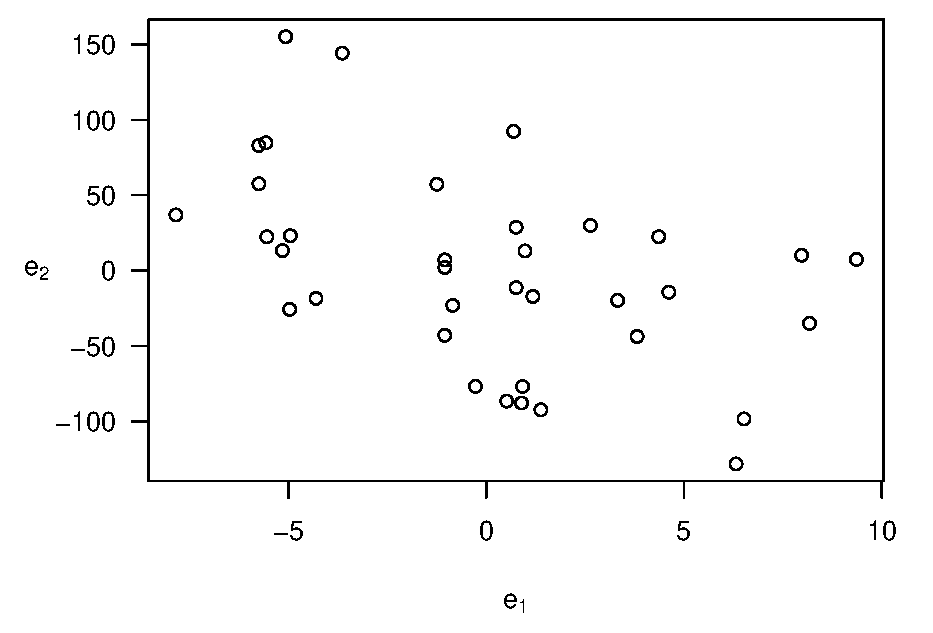
\includegraphics[width=.6\textwidth]{Chapter3/F3RefrigAddedVarPlot.eps}
    \caption{\label{F3:RefrigAddedVarPlot} \small  An added
variable plot. The residuals from the regression of PRICE on the
explanatory variables, omitting ECOST, are on the vertical axis. On
the horizontal axis are the residuals from the regression fit of
ECOST on the other explanatory variables. The correlation
coefficient is -0.48.}
  \end{center}
\end{figure}


The error $\varepsilon $ can be interpreted as the natural variation
in a sample. In many situations, this natural variation is small
compared to the patterns evident in the nonrandom regression
component. Thus, it is useful to think of the error, $\varepsilon_i
= y_i - \left( \beta_0 + \beta_1 x_{i1} + \ldots + \beta_k
x_{ik}\right) $, as the response after controlling for the effects
of the explanatory variables. In Section 3.3, we saw that a random
error can be approximated by a residual, $e_i = y_i - \left( b_0+b_1
x_{i1}+\cdots+b_k x_{ik}\right) $. Thus, in the same way, we may
think of a residual as the response after ``controlling for'' the
effects of the explanatory variables.

With this in mind, we can interpret the vertical axis of Figure
\ref{F3:RefrigAddedVarPlot} as the refrigerator PRICE controlled for
effects of RSIZE, FSIZE, SHELVES and FEATURES. Similarly, we can
interpret the horizontal axis as the ECOST controlled for effects of
RSIZE, FSIZE, SHELVES and FEATURES. The plot then provides a
graphical representation of the relation between PRICE and ECOST,
after controlling for the other explanatory variables. For
comparison, a scatter plot of PRICE and ECOST (not shown here) does
not control for other explanatory variables. Thus, it is possible
that the positive relationship between PRICE and ECOST is not due to
a causal relationship but rather one or more additional variables
that cause both variables to be large.

For example, from Table \ref{T3:RefrigSumStats}, we see that the
freezer size (FSIZE) is positively correlated with both ECOST and
PRICE. It certainly seems reasonable that increasing the size of a
freezer would cause both the energy cost and the price to increase.
Rather, the positive correlation may be due to the fact that large
values of FSIZE mean large values of both ECOST and PRICE.

Variables left out of a regression are called \emph{omitted
variables}. This omission could cause a serious problem in a
regression model fit; regression coefficients could be not only
strongly significant when they should not be, but they may also be
of the incorrect sign. Selecting the proper set of variables to be
included in the regression model is an important task; it is the
subject of Chapters 5 and 6.

\subsection{Partial Correlation Coefficients}\index{correlation coefficients!partial}

As we saw in Chapter 2, a correlation statistic is a useful quantity
for summarizing plots. The correlation for the added variable plot
is called a \emph{partial correlation coefficient}. It is defined to
be the correlation between the residuals $e_1$ and $e_2$ and is
denoted by $ r(y,x_j|x_1,\ldots,x_{j-1},x_{j+1},\ldots,x_k) $.
Because it summarizes an added variable plot, we may interpret $
r(y,x_j|x_1,\ldots,x_{j-1},x_{j+1},\ldots,x_k)$) to be the
correlation between $y$ and $x_j$, in the presence of the other
explanatory variables. To illustrate, the correlation between PRICE
and ECOST in the presence of the other explanatory variables is
-0.48.

The partial correlation coefficient can also be calculated using
\begin{equation}\label{E3:PartialCorr}
r(y,x_j | x_1 ,\ldots, x_{j-1}, x_{j+1}, \ldots, x_k) =
\frac{t(b_j)}{\sqrt{t(b_j)^2 + n-(k+1)}}.
\end{equation}

\noindent Here, $t(b_j)$ is the $t$-ratio for $b_j$ from a
regression of $y$ on $x_1,\ldots,x_k$ (including the variable
$x_j$). An important aspect of equation (\ref{E3:PartialCorr}) is
that it allows us to calculate partial correlation coefficients
running only one regression. For example, from Table
\ref{T3:RefrigFittedModel}, the partial correlation between PRICE
and ECOST in the presence of the other explanatory variables is
$(-3.1)/\sqrt{(-3.1)^2+37-(5+1)}\approx -0.48$.

Calculation of partial correlation coefficients is quicker when
using the relationship with the $t$-ratio, but may fail to detect
nonlinear relationships. The information in Table
\ref{T3:RefrigFittedModel} allows us to calculate all five partial
correlation coefficients in the Refrigerator Price Example after
running only one regression. The three-step procedure for producing
added variable plots requires ten regressions, two for each of the
five explanatory variables. Of course, by producing added variable
plots, we can detect nonlinear relationships that are missed by
correlation coefficients.

Partial correlation coefficients provide another interpretation for
$t$-ratios. Equation (\ref{E3:PartialCorr}) shows how to calculate a
correlation statistic from a $t$-ratio, thus providing another link
between correlation and regression analysis. Moreover, from equation
(\ref{E3:PartialCorr}) we see that the larger is the $t$-ratio, the
larger is the partial correlation coefficient. That is, a large
$t$-ratio means that there is a large correlation between the
response and the explanatory variable, controlling for other
explanatory variables. This provides a partial response to the
question that is regularly asked by consumers of regression
analyses, ``Which variable is most important?''

\section{Some Special Explanatory Variables}

The linear regression model is the basis of a rich family of models.
This section provides several examples to illustrate the richness of
this family. These examples demonstrate the use of (i) binary
variables, (ii) transformation of explanatory variables and (iii)
interaction terms. This section also serves to underscore the
meaning of the adjective \emph{linear} in the phrase ``linear
regression''; the regression function is linear in the parameters
but may be a highly nonlinear function of the explanatory variables.

\marginparjed{The linear regression function is linear in the
parameters but may be a highly nonlinear function of the explanatory
variables.}

\subsection{Binary Variables}\index{explanatory variable!binary}

Categorical variables provide a numerical label for measurements of
observations that fall in distinct groups, or \emph{categories}.
Because of the grouping, categorical variables are discrete and
generally take on a finite number of values. We begin our discussion
with a categorical variable that can take on one of only two values,
a \emph{binary} variable. Further discussion of categorical
variables is the topic of Chapter 4.


\linejed \index{datasets!term life insurance}

\textbf{Example: Term Life Insurance - Continued.} We now consider
the marital status of the survey respondent. In the Survey of
Consumer Finances, respondents can select among several options
describing their marital status including ``married,'' ``living with
a partner,'' ``divorced'' and so on. Marital status is not measured
continuously but rather takes on values that fall into distinct
groups. In this chapter, we group survey respondents according to
whether or not they are single, defined to include those who are
separated, divorced, widowed, never married, and are not married nor
living with a partner. Chapter 4 will present a more complete
analysis of marital status by including additional categories.

\marginparjed{Binary explanatory variables are also known as
indicator and dummy variables.}

The binary variable SINGLE is defined to be one if the survey
respondent is single and 0 otherwise. The variable SINGLE is also
known as an \emph{indicator} variable because it indicates whether
or not the respondent is single. Another name for this important
type of variable is a \emph{dummy} variable. We could use 0 and 100,
or 20 and 36, or any other distinct values. However, 0 and 1 are
convenient for the interpretation of the parameter values, discussed
below. To streamline the discussion, we now present a model using
only LNINCOME and SINGLE as explanatory variables.

\index{plots!letter}

For our sample of $n=275$ households, 57 are single and the other
218 are not.  To see the relationships among LNFACE, LNINCOME and
SINGLE, Figure \ref{F3:LinesLetterPlot} introduces a \emph{letter
plot} of LNFACE versus LNINCOME, with SINGLE as the code variable.
We can see that Figure \ref{F3:LinesLetterPlot} is a scatter plot of
LNFACE versus LNINCOME, using 50 randomly selected households from
our sample of 275 (for clarity of the graph). However, instead of
using the same plotting symbol for each observation, we have coded
the symbols so that we can easily understand the behavior of a third
variable, SINGLE. In other applications, you may elect to use other
plotting symbols such as $\clubsuit , \heartsuit , \spadesuit $, and
so on, or use different colors, to encode additional information.
For this application, the letter codes ``S'' for single and ``o''
for other were selected because they remind the reader of the plot
of the nature of the coding scheme. Regardless of the coding scheme,
the important point is that a letter plot is a useful device for
graphically portraying three or more variables in two dimensions.
The main restriction is that the additional information must be
categorized, such as with binary variables, to make the coding
scheme work.

\begin{figure}[htp]
  \begin{center}
    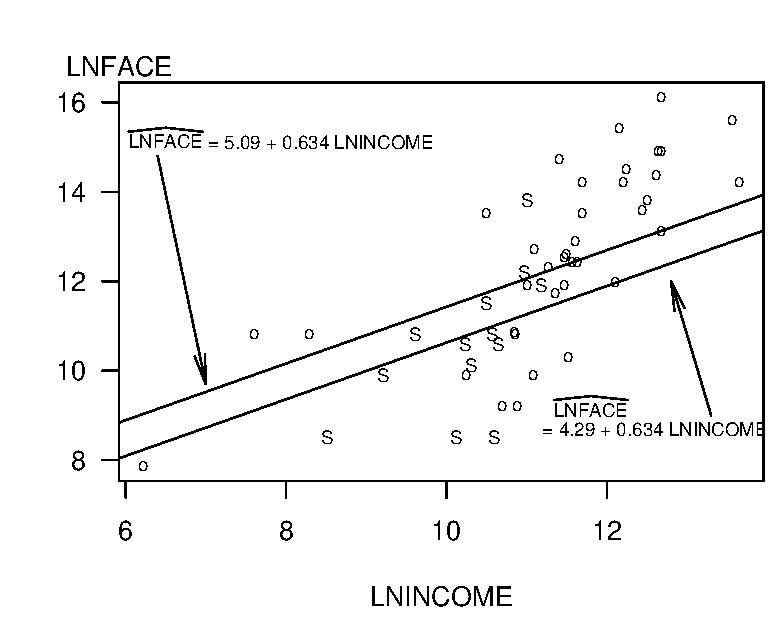
\includegraphics[width=.6\textwidth]{Chapter3/F3LinesLetterPlot.eps}
    \caption{\label{F3:LinesLetterPlot} \small Letter plot of LNFACE versus LNINCOME,
    with the letter code `S'' for single
and ``o'' for other. The fitted regression lines have been
superimposed. The lower line is for single and the upper line is for
other.}
  \end{center}
\end{figure}


Figure \ref{F3:LinesLetterPlot} suggests that LNFACE is lower for
those single than others for a given level of income. Thus, we now
consider a regression model, $LNFACE = \beta_0 + \beta_1 LNINCOME +
\beta_2 SINGLE + \varepsilon$. The regression function can be
written as:

\begin{equation*}
\textrm{E }y = \left\{ \begin{array}{ll}
        \beta_0 + \beta_1  \textrm{LNINCOME}           & \textrm{for other respondents} \\
        \beta_0 + \beta_2 + \beta_1  \textrm{LNINCOME} & \textrm{for single respondents}
\end{array} \right. .
\end{equation*}

The interpretation of the model coefficients differs from the
continuous variable case. For continuous variables such as LNINCOME,
we interpret $\beta_1$ as the expected change in $y$ per unit change
of logarithmic income, holding other variables fixed. For binary
variables such as SINGLE, we interpret $\beta_2$ as the expected
increase in $y$ when going from the base level of SINGLE (=0) to the
alternative level. Thus, although we have one model for both marital
statuses, we can interpret the model using two regression equations,
one for each type of marital status. By writing a separate equation
for each marital status, we have been able to simplify a complicated
multiple regression equation. Sometimes, you will find it easier to
communicate a series of simple relationships compared to a single,
complex relationship.

Although the interpretation for binary explanatory variables differs
from the continuous, the ordinary least squares estimation method
remains valid. To illustrate, the fitted version of the above model
is

\scalefont{0.9}
\begin{center}
\begin{tabular}{cclll}
  $\widehat{LNFACE}$ & = & 5.09   &  + 0.634 LNINCOME & - 0.800 SINGLE .\\
  std error    &   & (0.89) & ~~(0.078) & ~(0.248) \\
\end{tabular}
\end{center}
\scalefont{1.1111}


\noindent To interpret $b_2 = -0.800$, we say that we expect the
logarithmic face to be smaller by 0.80 for a survey respondent who
is single compared to the other category. This assumes that other
things, such as income, remain unchanged. For a graphical
interpretation, the two fitted regression lines are superimposed in
Figure \ref{F3:LinesLetterPlot}.

\linejed

\subsection{Transforming Explanatory Variables}\index{explanatory
variable!transformed}\index{transformations}

Regression models have the ability to represent complex,
\emph{nonlinear} relationships between the expected response and the
explanatory variables. For example, early regression texts, such as
Plackett (1960, Chapter 6) devote an entire chapter of material to
polynomial regression,
\begin{equation}\label{E3:polyregr}
\textrm{E } y  =  \beta_0 + \beta_1 x + \beta_2 x^2 + \ldots +
\beta_p x^p.
\end{equation}

\noindent Here, the idea is that a $p$th order polynomial in $x$ can
be used to approximate general, unknown nonlinear functions of $x$.

The modern day treatment of polynomial regression does not require
an entire chapter because the model in equation (\ref{E3:polyregr})
can be expressed as a special case of the linear regression model.
That is, with the regression function in equation
(\ref{E3:MLRegressionFct}), $\textrm{E } y = \beta_0 + \beta_1 x_1 +
\beta_2 x_2 + \ldots + \beta_k x_k$, we can choose $k = p$ and $x_1
= x, x_2 = x^2, \ldots, x_p = x^p$. Thus, with these choices of
explanatory variables, we can model a highly nonlinear function of
$x$.

We are not restricted to powers of $x$ in our choice of
transformations. For example, the model E $y = \beta_0 + \beta_1 \ln
 x$, provides another way to represent a gently sloping curve in
$x$. This model can be written as a special case of the basic linear
regression model using $x^{\ast} = \ln x$ as the transformed version
of $x$.

Transformations of explanatory variables need not be smooth
functions. To illustrate, in some applications, it is useful to
categorize a continuous explanatory variable. For example, suppose
that $x$ represents the number of years of education, ranging from 0
to 17. If we are relying on information self-reported by our sample
of senior citizens, there may be a substantial amount of error in
the measurement of $x$. We could elect to use a less informative,
but more reliable, transform of $x$ such as $x^{\ast}$, a binary
variable for finishing 13 years of school (finishing high school).
Formally, we would code $x^{\ast}$ = 1 if $x \geq 13$ and $x^{\ast}$
= 0 if $x < 13$.

Thus, there are several ways that nonlinear functions of the
explanatory variables can be used in the regression model. An
example of a nonlinear regression model is $y  =  \beta_0 + \exp
(\beta_1 x) + \varepsilon.$ These typically arise in science
applications of regressions where there are fundamental scientific
principles guiding the complex model development.


\subsection{Interaction Terms}\index{explanatory
variable!interaction}

We have so far discussed how explanatory variables, say $x_1$ and
$x_2$, affect the mean response in an additive fashion, that is, E
$y = \beta_0 + \beta_1 x_1 + \beta_2 x_2$. Here, we expect $y$ to
increase by $\beta_1$ per unit increase in $x_1$, with $x_2$ held
fixed. What if the marginal rate of increase of E $y$ differs for
high values of $x_2$ when compared to low values of $x_2$? One way
to represent this is to create an \emph{interaction variable} $x_3 =
x_1 \times x_2$ and consider the model E $y = \beta_0 + \beta_1 x_1
+ \beta_2 x_2 + \beta_3 x_3$.

With this model, the change in the expected $y$ per unit change in
$x_1$ now depends on $x_2$. Formally, we can assess small changes in
the regression function as

\begin{equation*}
\frac{\partial \textrm{E} y}{\partial x_1} =
\frac{\partial}{\partial x_1} \left(\beta_0 + \beta_1 x_1 + \beta_2
x_2 + \beta_3 x_1 x_2 \right) = \beta_1 + \beta_3 x_2 .
\end{equation*}
In this way, we may allow for more complicated functions of $x_1$
and $x_2$. Figure \ref{F3:Interaction} illustrates this complex
structure. From this figure and the above calculations, we see that
the partial changes of E $y$ due to movement of $x_1$ depend on the
value of $x_2$. In this way, we say that the partial changes due to
each variable are not unrelated but rather ``move together.''


\begin{figure}[htp]
  \begin{center}
    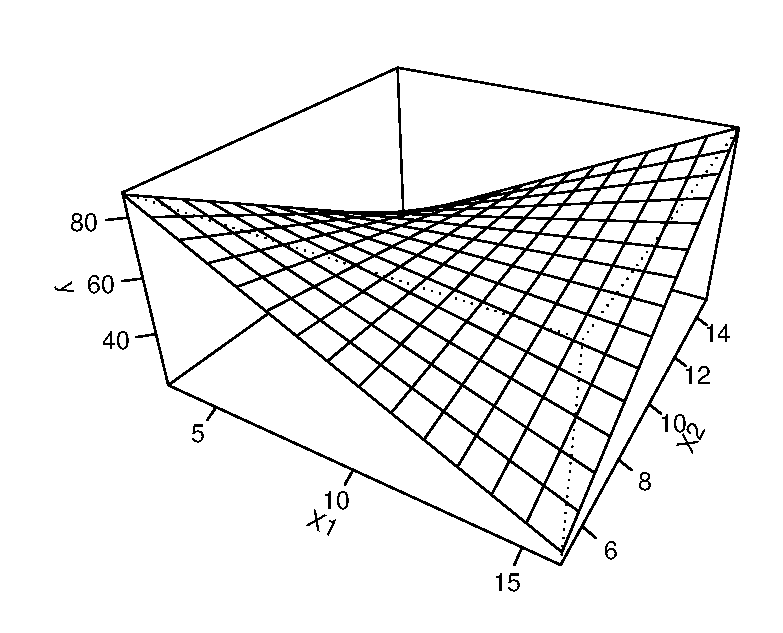
\includegraphics[width=.6\textwidth]{Chapter3/F3Interaction.eps}
    \caption{\label{F3:Interaction} \small Plot of E $y = \beta_0 +
         \beta_1 x_1 + \beta_2 x_2 + \beta_3 x_1 x_2$ versus $x_1$ and
          $x_2$.}
  \end{center}
\end{figure}

More generally, an interaction term is a variable that is created as
a nonlinear function of two or more explanatory variables. These
special terms, even though permitting us to explore a rich family of
nonlinear functions, can be cast as special cases of the linear
regression model. To do this, we simply create the variable of
interest and treat this new term as another explanatory variable. Of
course, not every variable that we create will be useful. In some
instances, the created variable will be so similar to variables
already in our model that it will provide us with no new
information. Fortunately, we can use $t$-tests to check whether the
new variable is useful. Further, Chapter 4 will introduce a test to
decide whether a group of variables is useful.

The function that we use to create an interaction variable must be
more than just a linear combination of other explanatory variables.
For example, if we use $x_3 = x_1 + x_2$, we will not be able to
estimate all of the parameters. Chapter 5 will introduce some
techniques to help avoid situations when one variable is a linear
combination of the others.

To give you some exposure to the wide variety of potential
applications of special explanatory variables, we now present a
series of short examples.

\bigskip

\linejed

\textbf{Example: Term Life Insurance - Continued.} How do we
interpret the interaction of a binary variable with a continuous
variable? To illustrate, consider a Term Life regression model,
$\textrm{LNFACE} = \beta_0 + \beta_1 \textrm{LNINCOME} + \beta_2
\textrm{SINGLE} + \beta_2 \textrm{LNINCOME*SINGLE} + \varepsilon$.
In this model, we have created a third explanatory variable through
the interaction of LNINCOME and SINGLE. The regression function can
be written as:
\begin{equation*}
\textrm{E }y = \left\{ \begin{array}{ll}
        \beta_0 + \beta_1  \textrm{LNINCOME}           & \textrm{for other respondents} \\
        \beta_0 + \beta_2 + (\beta_1 + \beta_3)  \textrm{LNINCOME} & \textrm{for single respondents}
\end{array} \right. .
\end{equation*}
Thus, through this single model with four parameters, we can create
two separate regression lines, one for those single and one for
others. Figure \ref{F3:LetterInteract} shows the two fitted
regression lines for our data.


\begin{figure}[htp]
  \begin{center}
    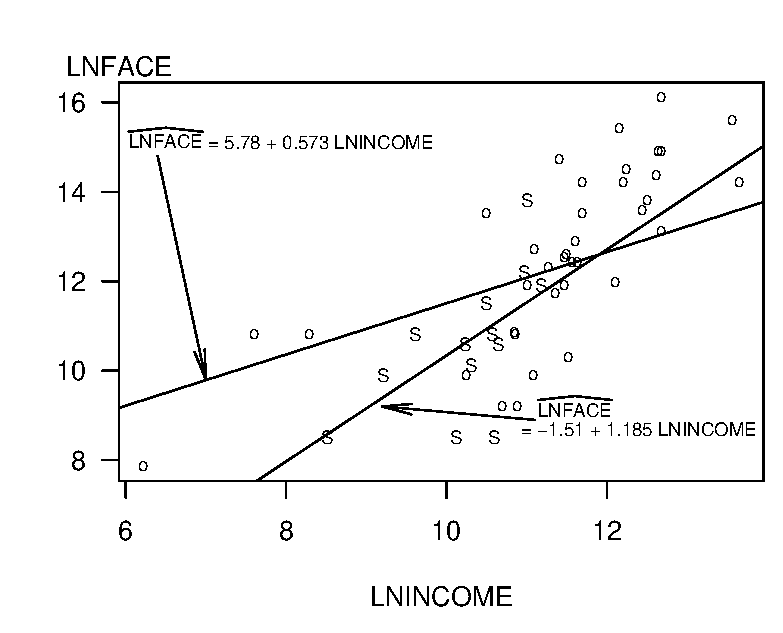
\includegraphics[width=0.6\textwidth]{Chapter3/F3LetterInteract.eps}
    \caption{\label{F3:LetterInteract} \small Letter plot of LNFACE versus LNINCOME,
    with the letter code `S'' for single
and ``o'' for other. The fitted regression lines have been
superimposed. The lower line is for single and the upper line is for
other.}
  \end{center}
\end{figure}

\linejed \index{examples!life insurance company expenses}

\textbf{Example: Life Insurance Company Expenses.}\ecaptionjed{Life
Insurance Company Expenses} In a well-developed life insurance
industry, minimizing expenses is critical for a company's
competitive position. Segal (2002) analyzed annual accounting data
from over 100 firms for the period 1995-1998, inclusive, using a
data base from the National Association of Insurance Commissioners
(NAIC) and other reported information. Segal modeled overall company
expenses as a function of firm outputs and the price of inputs. The
outputs consist of insurance production, measured by $x_1$ through
$x_5$, described in Table \ref{T3:Expenses}. Segal also considered
the square of each output, as well as an interaction term with a
dummy/binary variable $D$ that indicates whether or not the firm
uses a branch company to distribute its products. (In a branch
company, field managers are company employees, not independent
agents.)\index{actuarial \& financial terms and concepts!insurance
company branch office}

\scalefont{0.9}
\begin{center}  \begin{table}[h] \caption{\label{T3:Expenses}
Twenty-Three Regression Coefficients from an Expense Cost Model}
\begin{tabular}{l|rrrr}
\hline
 &  \multicolumn{2}{c}{Variable} &  \multicolumn{2}{c}{Variable
 Squared} \\
  &  Baseline &  Interaction  &  Baseline &  Interaction \\
  &   &   with~~   &   &   with~~  \\
Variable & $(D=0)$ &  $(D=1)$ & $(D=0)$ &  $(D=1)$\\
\hline Number of Life Policies Issued ($x_1$)     &  -0.454 & 0.152
& 0.032
& -0.007 \\
Amount of Term Life Insurance Sold ($x_2$)  & 0.112 & -0.206 & 0.002
& 0.005 \\
Amount of Whole Life Insurance Sold ($x_3$) & -0.184 & 0.173 & 0.008
& -0.007 \\
Total Annuity Considerations ($x_4$)        & 0.098 & -0.169 &
-0.003 & 0.009 \\
Total Accident and Health Premiums ($x_5$)  &-0.171 & 0.014 & 0.010
& 0.002 \\
Intercept  & 7.726 & & & \\
Price of Labor (PL) & 0.553 & & & \\
Price of Capital (PC) & 0.102 & & & \\
\hline
\end{tabular}
\newline
\flushleft ~~~Note: $x_1$ through $x_5$ are in logarithmic units.
\textit{Source: Segal (2002)}
\end{table}  \end{center}  \scalefont{1.1111}
For the price inputs, the price of labor ($PL$) is defined to be the
total cost of employees and agents divided by their number, in
logarithmic units. The price of capital ($PC$) is approximated by
the ratio of capital expense to the number of employees and agents,
also in logarithmic units. The price of materials consists of
expenses other than labor and capital divided by the number of
policies sold and terminated during the year. It does not appear
directly as an explanatory variable. Rather, Segal took the
dependent variable ($y$) to be total company expenses divided by the
price of materials, again in logarithmic units.

With these variable definitions, Segal estimated the following
regression function.
\begin{equation*}
\mathrm{E~}y=\beta_0 + \sum_{j=1}^5 \left( \beta_j x_j + \beta_{j+5}
D x_j + \beta_{j+10} x_j^2 + \beta_{j+15}D x_j^2  \right) +
\beta_{21} PL + \beta_{22} PC.
\end{equation*}
The parameter estimates appear in Table \ref{T3:Expenses}. For
example, the marginal change in E $y$ per unit change in $x_1$ is
\begin{equation*}
\frac{\partial ~ \mathrm{E}y}{\partial x_1}= \beta_1 + \beta_{6} D +
2 \beta_{11} x_1 + 2 \beta_{16}D x_1,
\end{equation*}
which is estimated as $ -0.454 + 0.152 D + (0.064 - 0.014 D) x_1$.
For these data, the median number of policies issued was
$x_1=15,944$. At this value of $x_1$, the estimated marginal change
is $ -0.454 + 0.152 D + (0.064 - 0.014 D) \mathrm{ln}(15944) = 0.165
+ 0.017 D,$ or 0.165 for baseline $(D=0)$ and 0.182 for branch
$(D=1)$ companies.

These estimates are elasticities, as defined in Section 3.2.2. To
interpret these coefficients further, let $COST$ represent total
general company expenses and $NUMPOL$ represent the number of life
policies issued. Then, for branch $(D=1)$ companies, we have
\begin{equation*}
0.182 \approx \frac{\partial y }{\partial x_1 } = \frac{\partial ~
\mathrm{ln}~COST}{\partial ~ \mathrm{ln}~NUMPOL}= \frac{
\frac{\partial ~ COST}{\partial ~NUMPOL}} {\frac{COST}{NUMPOL}},
\end{equation*}
or $\frac{\partial ~ COST}{\partial ~NUMPOL} \approx 0.182
\frac{COST}{NUMPOL}$. The median cost is \$15,992,000, so the
marginal cost per policy at these median values is $ 0.182 \times
(15992000/15944) = \$182.55$.

\linejed


\bigskip

\textbf{Special Case: Curvilinear Response Functions}. We can expand
the polynomial functions of an explanatory variable to include
several explanatory variables. For example, the expected response,
or \emph{response function}, for a second-order model with two
explanatory variables is\index{response function}

\begin{equation*}
\textrm{E} y = \beta_0 + \beta_1 x_1 + \beta_2 x_2 + \beta_{11}
x_1^2 + \beta_{22} x_2^2 + \beta_{12} x_1 x_2.
\end{equation*}


Figure \ref{F3:Curvilinear} illustrates this response function.
Similarly, the response function for a second-order model with three
explanatory variables is

\begin{equation*}
\textrm{E} y = \beta_0 + \beta_1 x_1 + \beta_2 x_2 + \beta_3 x_3 +
\beta_{11} x_1^2 + \beta_{22} x_2^2 + \beta_{33} x_3^2 + \beta_{12}
x_1 x_2 + \beta_{13} x_1 x_3 + \beta_{23} x_2 x_3.
\end{equation*}

When there is more than one explanatory variable, third and higher
order models are rarely used in applications.


\begin{figure}[htp]
  \begin{center}
    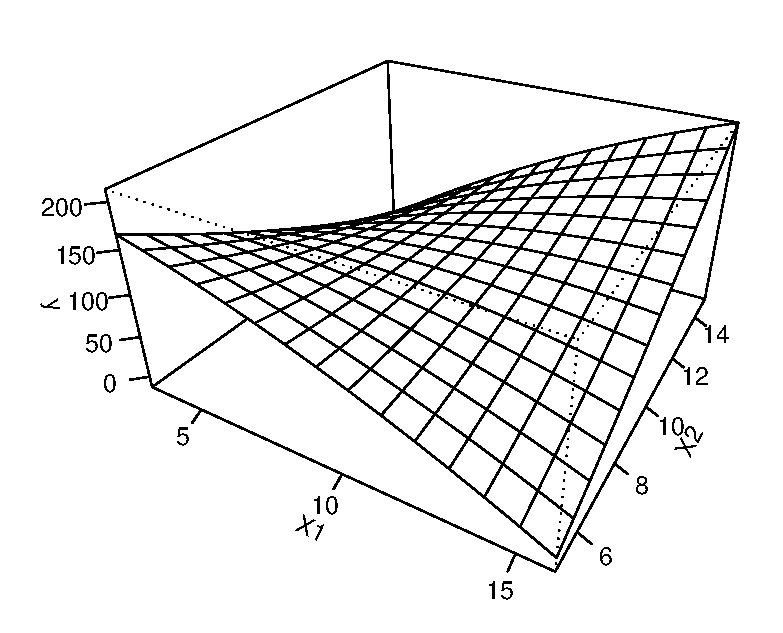
\includegraphics[width=.6\textwidth]{Chapter3/F3Curvilinear.eps}
    \caption{\label{F3:Curvilinear} \small Plot of E $y = \beta_0 + \beta_1 x_1 + \beta_2 x_2 +
     \beta_{11} x_1^2 + \beta_{22} x_2^2 + \beta_{12} x_1 x_2$ versus
$x_1$ and $x_2$.}
  \end{center}
\end{figure}

\bigskip

\textbf{Special Case: Nonlinear Functions of a Continuous Variable}.
In some applications, we expect the response to have some abrupt
changes in behavior at certain values of an explanatory variable,
even if the variable is continuous. For example, suppose that we are
trying to model an individual's charitable contributions ($y$) in
terms of their wages ($x$). For 2007 data, a simple model we might
entertain is given in Figure \ref{F3:Charity}.


\begin{figure}[htp]
  \begin{center}
    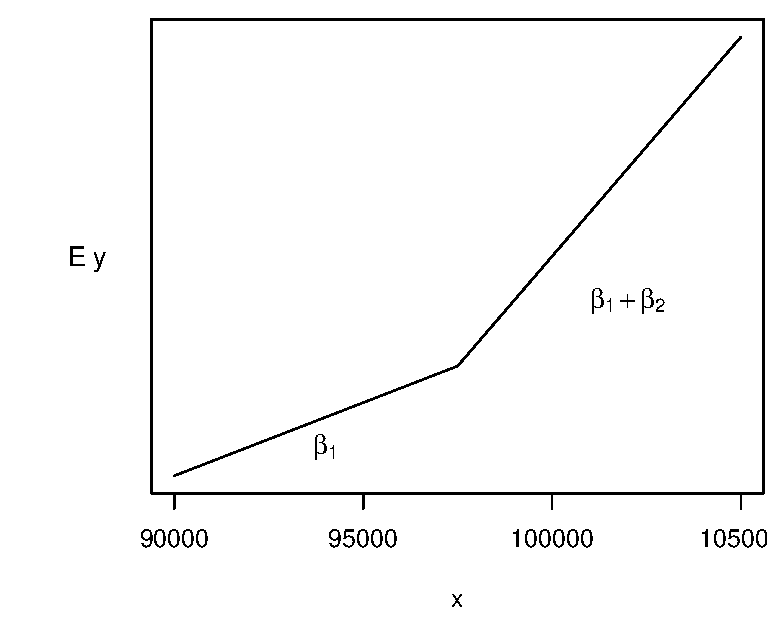
\includegraphics[width=.6\textwidth]{Chapter3/F3Charity.eps}
    \caption{\label{F3:Charity} \small The marginal change in E $y$ is
    lower below \$97,500. The parameter $\beta_2$ represents the
    difference in the slopes.}
  \end{center}
\end{figure}


A rational for this model is that, in 2007 individuals paid 7.65\%
of their income for Social Security taxes up to \$97,500. No social
security taxes are excised on wages in excess of \$97,500. Thus, one
theory is that, for wages in excess of \$97,500, individuals have
more disposal income per dollar and thus should be more willing to
make charitable contributions.

To model this relationship, define the binary variable $z$ to be
zero if $x < 97,500$ and to be one if $x \geq  97,500$. Define the
regression function to be E $y = \beta_0 + \beta_1 x + \beta_2 z (x
- 97,500).$ This can be written as:


\begin{equation*}
\textrm{E }y = \left\{ \begin{array}{ll}
        \beta_0 + \beta_1  x                    & x < 97,500 \\
        \beta_0 - \beta_2(97,500) + (\beta_1+\beta_2) x & x \geq  97,500
\end{array} . \right.
\end{equation*}

\noindent To estimate this model, we would run a regression of $y$
on two explanatory variables, $x_1 = x$ and $x_2 = z \times (x -
97,500)$. If $\beta_2 > 0,$ then the marginal rate of charitable
contributions is higher for incomes exceeding \$97,500.

Figure \ref{F3:Charity} illustrates this relationship, known as
\emph{piecewise linear regression} or sometimes a ``broken stick''
model. The sharp break in Figure \ref{F3:Charity} at $x = 97,500$ is
called a ``kink.'' We have linear relationships above and below the
kinks and have used a binary variable to put the two pieces
together. We are not restricted to one kink. For example, suppose
that we wish to do a historical study of Federal taxable income for
1992 single filers. Then, there were three tax brackets: the
marginal tax rate below \$21,450 was 15\%, above \$51,900 was 31\%,
and in between was 28 percent. For this example, we would use two
kinks, at 21,450 and 51,900.\index{regression model!piecewise
linear}\index{regression model!broken stick}

Further, piecewise linear regression is not restricted to continuous
response functions. For example, suppose that we are studying the
commissions paid to stockbrokers ($y$) in terms of the number of
shares purchased by a client ($x$). We might expect to see the
relationship illustrated in Figure \ref{F3:Break}. Here, the
discontinuity at $x = 100$ reflects the administrative expenses of
trading in odd lots, as trades of less than 100 shares are called.
The lower marginal cost for trades in excess of 100 shares simply
reflects the economies of scale for doing business in larger
volumes. A regression model of this is E $y = \beta_0 + \beta_1 x +
\beta_2 z + \beta_3 z x$ where $z = 0$ if $x < 100$ and $z = 1$ if
$x \geq 100$. The regression function depicted in Figure
\ref{F3:Break} is

\begin{equation*}
\textrm{E }y = \left\{ \begin{array}{ll}
        \beta_0 + \beta_1  x_1                    & x<100 \\
        \beta_0 + \beta_2 + (\beta_1+\beta_3) x_1 & x \geq 100
\end{array} . \right.
\end{equation*}

\begin{figure}[htp]
  \begin{center}
    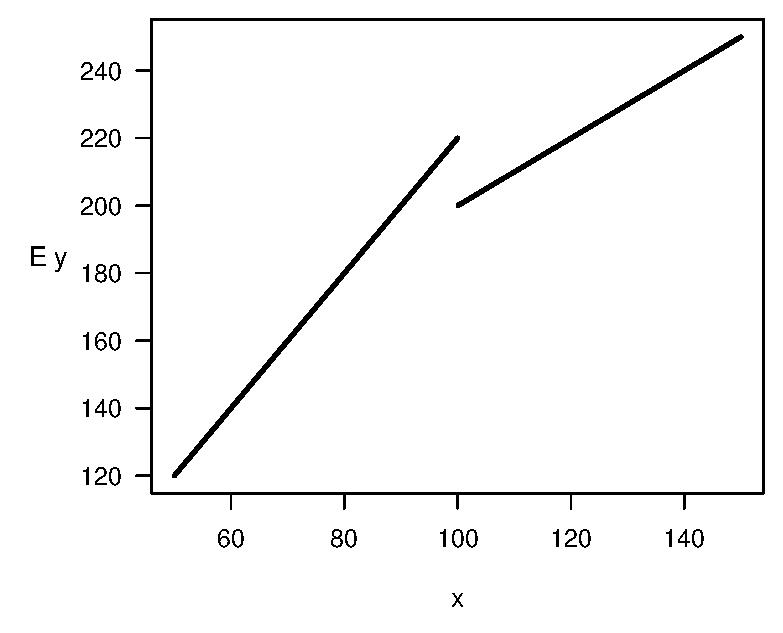
\includegraphics[width=.6\textwidth]{Chapter3/F3Break.eps}
    \caption{\label{F3:Break} \small Plot of expected commissions (E $y$) versus number of shares traded ($x$).
    The break at $x=100$ reflects savings in administrative expenses.
    The lower slope for $x \geq 100$ reflects economies of scales in expenses.}
  \end{center}
\end{figure}


\section{Further Reading and References}

For proofs of the Chapter 3 results, we refer the reader to
Goldberger (1991). Nonlinear regression models are discussed in, for
example, Bates and Watts (1988).

Chapter 3 has introduced the fundamentals of multiple linear
regression. Chapter 4 will widen the scope by introducing
categorical variables and statistical inference methods for handling
several coefficients simultaneously. Chapter 5 will introduce
techniques to help you pick appropriate variables in a multiple
linear regression model. Chapter 6 is a synthesis chapter,
discussing model interpretation, variable selection and data
collection.

\bigskip


\textbf{Chapter References}

\begin{multicols}{2}

\scalefont{0.9}

Bates, Douglas M. and Watts, D. G. (1988). \textit{Nonlinear
Regression Analysis and its Applications}. John Wiley \& Sons, New
York.

Lemaire, Jean (2002). Why do females live longer than males?
\textit{North American Actuarial Journal} 6(4), 21-37.

Goldberger, Arthur (1991). \textit{A Course in Econometrics}.
Harvard University Press, Cambridge.

Plackett, R.L. (1960). \textit{Regression Analysis}. Clarendon
Press, Oxford, England.

Segal, Dan (2002). An economic analysis of life insurance company
expenses. \textit{North American Actuarial Journal} 6(4), 81-94.

\scalefont{1.1111}

\end{multicols}

\bigskip


\section{Exercises}

\begin{exercises}

\scalefont{0.90}

\item  Consider a fictitious data set of $n = 100$ observations with
$s_y = 80$. We run a regression with three explanatory variables to
get $s = 50$.

a.  Calculate the adjusted coefficient of determination, $R_a^2$.

b. Complete the ANOVA table.

\begin{center}
\begin{tabular}{l|lcl}
\hline \multicolumn{4}{c}{ANOVA\ Table} \\ \hline Source & Sum of
Squares & $df$ & Mean Square \\ \hline
Regression & &  & \\
Error &  &  &  \\
Total &  &  &  \\ \hline
\end{tabular}
\end{center}

c.  Calculate the (unadjusted) coefficient of determination, $R^2$.

\item  Consider a fictitious data set of $n = 100$
observations with $s_y = 80$. We run a regression with three
explanatory variables to get $s = 50$. We also get
\begin{equation*}
\left(\mathbf{X^{\prime} X} \right)^{-1} = \left(
\begin{array}{cccc}
100 & 20 &20 & 20\\
20 & 90 & 30 & 40 \\
20 & 30 & 80 & 50 \\
20 & 40 & 50 & 70 \\
\end{array}
\right).
\end{equation*}

a. Determine the standard error of $b_3$, $se(b_3)$.

b. Determine the estimated covariance between $b_2$ and $b_3$.

c. Determine the estimated correlation between $b_2$ and $b_3$.

d. Determine the estimated variance of $4b_2 + 3b_3$.

\item Consider the following small fictitious data set. You will be
fitting a regression model to $y$ using two explanatory variables,
$x_1$ and $x_2$.

\begin{center}
\begin{tabular}{c|cccc}
\hline $i$ & 1 & 2 & 3 & 4 \\
$x_{i,1}$ & -1 & 2 & 4 & 6 \\
$x_{i,2}$ & 0 & 0 & 1 & 1 \\
$y_i$ & 0 & 1 & 5 & 8 \\
 \hline
\end{tabular}
\end{center}

\noindent From the fitted regression model, we have $s = 1.373$ and
\begin{equation*}
\mathbf{b} = \left(
\begin{array}{c}
0.15 \\ 0.692 \\2.88
\end{array}
\right) ~~~\mathrm{and}~~~ \left(\mathbf{X^{\prime} X} \right)^{-1}
= \left(
\begin{array}{cccc}
0.53846 & -0.07692 &-0.15385\\
-0.07692 & 0.15385 & -0.69231 \\
-0.15385 & -0.69231 & 4.11538 \\
\end{array}
\right).
\end{equation*}

a. Write down the vector of dependent variables, $\mathbf{y}$, and
the matrix of explanatory variables, $\mathbf{X}$.

b. Determine the numerical value for $\widehat{y}_3$, the fitted
value for the third observation.

c. Determine the numerical value for $se(b_2)$.

d. Determine the numerical value for $t(b_1)$.

\empexjed{WiscLottery}\index{datasets!Wisconsin lottery sales}

\item \textbf{Wisconsin Lottery.}\label{Ex:Lottery3}
Section 2.1 described a sample of $n=50$ geographic areas (zip
codes) containing sales data on the Wisconsin state lottery ($y =
SALES$). In that section, sales were analyzed using a basic linear
regression model with $x = POP$, the area population, as the
explanatory variable. This exercise extends that analysis by
introducing additional explanatory variables given in Table
\ref{Ex:LotVariables}.


\begin{table}[h]
\scalefont{0.8}
 \caption{\label{Ex:LotVariables} \small Lottery,
economic and demographic characteristics of fifty Wisconsin ZIP
codes}
\begin{center}
\begin{tabular}{ll}
\hline
\multicolumn{ 2}{c}{{\bf Lottery characteristics}} \\
  SALES  & Online lottery sales to individual consumers \\
\hline
\multicolumn{ 2}{c}{{\bf Economic and demographic characteristics}} \\
 PERPERHH  & Persons per household  \\
 MEDSCHYR  & Median years of schooling  \\
   MEDHVL  & Median home value in \$1000s for owner-occupied homes \\
 PRCRENT   & Percent of housing that is renter occupied \\
 PRC55P    & Percent of population that is 55 or older \\
 HHMEDAGE  & Household median age \\
MEDINC      & Estimated median household income, in \$1000s \\
POP   & Population, in thousands \\
\hline

\end{tabular}
\scalefont{1.25}
\end{center}
\end{table}

a. Produce a table of summary statistics for all variables. One zip
code (observation 11, zip = 53211, Shorewood Wisconsin a suburb of
Milwaukee) appears to have unusually large values of MEDSCHYR and
MEDHVL. For this observation, how many standard deviations is the
value of MEDSCHYR above the mean? For this observation, how many
standard deviations is the value of MEDHVL above the mean?

b. Produce a table of correlations. What three variables are most
highly correlated with SALES?

c. Produce a scatter plot matrix of all explanatory variables and
SALES. In the plot of MEDSCHYR versus SALES, describe the position
of observation 11.

d. Fit a linear model of SALES on all eight explanatory variables.
Summarize the fit of this model by citing the residual standard
deviation, $s$, the coefficient of determination, $R^2$ and its
adjusted version, $R^2_a$.

e. Based on your part (d) model fit, is MEDSCHYR a statistically
significant variable? To respond to this question, use a formal test
of hypothesis. State your null and alternative hypotheses, decision
making criterion and your decision-making rule.

f. Now fit a more parsimonious model, using SALES as the dependent
variable and MEDSCHYR, MEDHVL and POP as explanatory variables.
Summarize the fit of this model by citing the residual standard
deviation, $s$, the coefficient of determination, $R^2$ and its
adjusted version, $R^2_a$. How do these values compare to the model
fit in part (d)?

g. Note that the sign of the regression coefficient associated with
MEDSCHYR is now negative. To help interpret this coefficient,
compute the corresponding partial correlation coefficient. What is
the interpretation of this coefficient.

h. To get further insights into the relation between MEDSCHYR and
SALES, produce an added variable plot controlling for the effects of
MEDHVL and POP. Check that the correlation associated with this plot
agrees with your answer in part (g).

i. Re-run the regression in part (f), after removing observation 11.
Cite the basic summary statistics from this regression. For this
model fit, is MEDSCHYR a statistically significant variable? To
respond to this question, use a formal test of hypothesis. State
your null and alternative hypotheses, decision making criterion and
your decision-making rule.

j. Re-run the regression in part (f), after removing observation 9.
Cite the basic summary statistics from this regression.

\empexjed{NAICExpense}\index{datasets!insurance company expenses}

\item \textbf{Insurance company expenses.}\label{Ex:NAICExpense3}
This exercise considers insurance company data from the NAIC and
described in Exercise 1.\ref{Ex:NAICExpense}.

Table \ref{Ex:NAICVariables} describes several variables that can be
used to explain expenses. As with Segal's (2002) study of life
insurers, firm ``outputs'' consist of premiums written (for property
and casualty, these are subdivided into personal and commercial
lines) as well as losses (subdivided into short and long tail
lines). ASSETS and CASH are commonly used measures of the size of a
company. GROUP, STOCK and MUTUAL describe the organizational
structure. Firm ``inputs'' were gathered from the Bureau of Labor
Statistics (BLS, from the Occupational Employee Statistics program).
WAGESTAFF is calculated as the average wage in the state where the
insurance company headquartered. AGENTWAGE is calculated as the
weighted average of annual wages of the brokerage industry, weighted
by the percentage of gross premium written in each state.




\begin{table}[h]
\scalefont{0.8} \caption{\label{Ex:NAICVariables} \small Insurer
Expense Variables}
\begin{tabular}{l|l}
\hline
\bf Variable & \multicolumn{1}{c} {\bf Description} \\
\hline
\multicolumn{2}{c} {\bf NAIC Variables } \\
\hline
EXPENSES & Total expenses incurred, in millions of dollars \\
    LOSSLONG & Losses incurred for long tail lines, in millions of dollars \\
    LOSSSHORT& Losses incurred for short tail lines, in millions of dollars \\
GPWPERSONAL & Gross premium written for personal lines, in millions of dollars \\
  GPWCOMM  & Gross premium written for commercial lines, in millions of dollars \\
ASSETS & Net admitted assets, in millions of dollars \\
CASH & Cash and invested assets, in millions of dollars \\
      GROUP & Indicates if the company is affiliated  \\
      STOCK & Indicates if the company is a stock company \\
     MUTUAL & indicates if the company is a mutual company \\
\hline \multicolumn{2}{c} {\bf BLS Variables } \\ \hline
STAFFWAGE & Annual average wage of the insurer's administrative staff,  \\
 & ~~~~in thousands of dollars  \\
AGENTWAGE & Annual average wage of the insurance agent, in thousands of dollars \\
\hline

\end{tabular}
\scalefont{1.25}
\end{table}

\bigskip

A preliminary inspection of the data showed that many firms did not
report any insurance losses incurred in 2005. For this exercise, we
consider the 384 companies with some losses in the file
``NAICExpense.csv''.

a. Produce summary statistics of the response variable and the
(non-binary) explanatory variables. Note the pattern of skewness for
each variable. Note that many variables have negative values.

b. Transform each non-binary variable through the modified logarithm
transform, $\ln(1+x)$. Produce summary statistics of these modified
non-binary explanatory variables. Let LNEXPENSES
($=\ln(1+EXPENSES)$) denote the modified expense variable.

For subsequent analysis, use only the modified variables described
in part (b).

c. Produce a table of correlations for the non-binary variables.
What three variables are most highly correlated with LNEXPENSES?

d. Provide a boxplot of LNEXPENSES by level of GROUP. Which level of
group has higher expenses?

e. Fit a linear model of LNEXPENSES on all eleven explanatory
variables. Summarize the fit of this model by citing the residual
standard deviation, $s$, the coefficient of determination, $R^2$ and
its adjusted version, $R^2_a$.

f. Fit a linear model of LNEXPENSES on a reduced model using eight
explanatory variables, dropping CASH, STOCK and MUTUAL. For the
explanatory variables, include assets, GROUP, both versions of
losses and gross premiums, as well as the two BLS variables.

f(i). Summarize the fit of this model by citing $s$, $R^2$ and
$R^2_a$.

f(ii). Interpret the coefficient associated with commercial lines
gross premiums on the logarithmic scale.

f(iii). Suppose that GPWCOMM increases by \$1, how much do we expect
EXPENSES to increase? Use your answer in part f(ii) and median
values of GPWCOMM and EXPENSES for this question.

g. Square each of the two loss and the two gross premium variables.
Fit a linear model of LNEXPENSES on a reduced model using twelve
explanatory variables, the eight variables in part (f) and the four
additional squared terms just created.

g(i). Summarize the fit of this model by citing  $s$,  $R^2$ and
$R^2_a$.

g(ii). Do the quadratic variables appear to be useful explanatory
variables?\index{explanatory variable!quadratic}


h. Now omit the two BLS variables, so you are fitting a model of
LNEXPENSES on assets, GROUP, both versions of losses and gross
premiums, as well as quadratic terms. Summarize the fit of this
model by citing $s$, $R^2$ and $R^2_a$. Comment on the number of
observations used to fit this model compared to part (f).

i. Drop the quadratic terms in part (g) and add interaction terms
with the dummy variable GROUP. Thus, there are now eleven variables,
assets, GROUP, both versions of losses and gross premiums, as well
as interactions of GROUP with assets and both versions of losses and
gross premiums.

i(i). Summarize the fit of this model by citing $s$, $R^2$ and
$R^2_a$.

i(ii). Suppose that GPWCOMM increases by \$1, how much do we expect
EXPENSES to increase for GROUP=0 companies? Use the median values of
GPWCOMM and EXPENSES of GROUP=0 companies for this question.

i(iii). Suppose that GPWCOMM increases by \$1, how much do we expect
EXPENSES to increase for GROUP=1 companies? Use the median values of
GPWCOMM and EXPENSES of GROUP=1 companies for this question.

\empexjed{UNLifeExpectancy}\index{datasets!national life
expectancies}

\item \textbf{National Life Expectancies.}\label{Ex:UNLIFE3} We
continue the analysis begun in Exercises 1.\ref{Ex:UNLIFE} and
2.\ref{Ex:UNLIFE2}. Now fit a regression model on LIFEEXP using
three explanatory variables, FERTILITY, PUBLICEDUCATION and lnHEALTH
(the natural logarithmic transform of PRIVATEHEALTH).

a. Interpret the regression coefficient associated with public
education.

b. Interpret the regression coefficient associated with health
expenditures without using the logarithmic scale for expenditures.

c. Based on the model fit, is PUBLICEDUCATION a statistically
significant variable? To respond to this question, use a formal test
of hypothesis. State your null and alternative hypotheses,
decision-making criterion and your decision-making rule.

d. The negative sign of the PUBLICEDUCATION coefficient is
surprising, in that the sign of the correlation between
PUBLICEDUCATION and LIFEEXP is positive and intuition suggests a
positive relation. To check this result, an added variable plot
appears in Figure~\ref{Ex:UNLIFEPlot2}.

d(i). For an added variable plot, describe its purpose and a method
for producing it.

d(ii). Calculate the correlation corresponding to the added variable
plot that appears in Figure~\ref{Ex:UNLIFEPlot2}.

\begin{figure}[htp]
  \begin{center}
   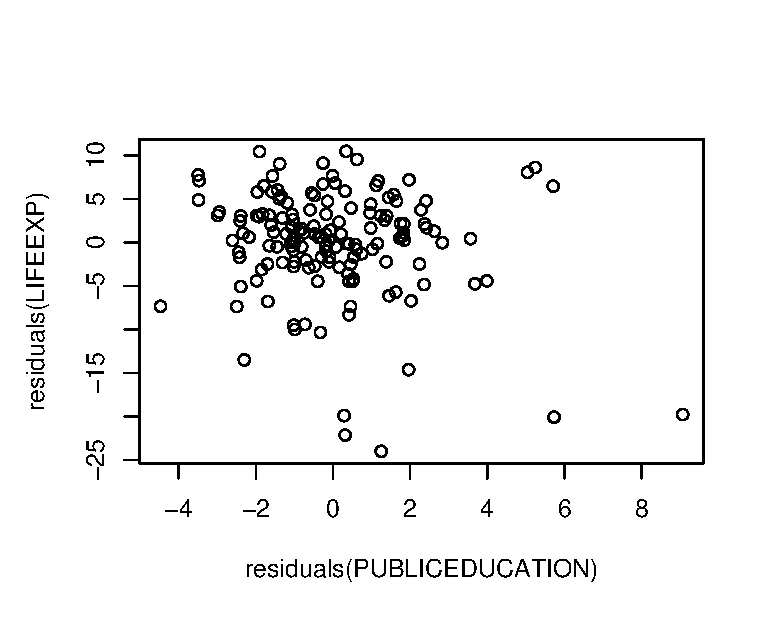
\includegraphics[width=.6\textwidth]{Chapter3/UNLIFE2.eps}
   \caption{\label{Ex:UNLIFEPlot2} \small  Added variable plot of PUBLICEDUCATION  versus LIFEEXP,
   controlling for FERTILITY and lnHEALTH.}
  \end{center}
\end{figure}


\scalefont{1.1111}
\end{exercises}

\setcounter{chapter}{3}
\chapter{Multiple Linear Regression - II}


{\small \textit{Chapter Preview}. This chapter extends the
discussion of multiple linear regression by introducing statistical
inference for handling several coefficients simultaneously. To
motivate this extension, this chapter considers coefficients
associated with \textit{categorical variables}. These variables
allow us to group observations into distinct categories. This
chapter shows how to incorporate categorical variables into
regression functions using binary variables, thus widening the scope
of potential applications. Statistical inference for several
coefficients allows analysts to make decisions about categorical
variables, as well as other important applications. Categorical
explanatory variables also provide the basis for an \textit{ANOVA}
model, a special type of regression model that permits easier
analysis and interpretation.}

\section{The Role of Binary Variables}\label{S4:BinaryVar}

\marginparjed{Categorical variables provide labels for observations
to denote membership in distinct groups, or categories.}

\index{explanatory variable!categorical}\index{explanatory
variable!factor}\index{categorical variable}

\textit{Categorical variables} provide labels for observations to
denote membership in distinct groups, or categories. A binary
variable is a special case of a categorical variable. To illustrate,
a binary variable may tell us whether or not someone has health
insurance. A categorical variable could tell us whether someone has
\begin{itemize}
\item private group insurance (offered by employers and
associations), \item private individual health insurance (through
insurance companies), \item public insurance (such as Medicare or
Medicaid) or \item no health insurance.
\end{itemize}

\noindent For categorical variables, there may or may not be an
ordering of the groups. In health insurance, it is difficult to
order these four categories and say which is ``larger,'' private
group, private individual, public or no health insurance. In
contrast, for education, we might group individuals into ``low,''
``intermediate'' and ``high'' years of education. In this case,
there is an ordering among groups based on level of educational
achievement. As we will see, this ordering may or may not
provide information about the dependent variable. \textit{Factor} is
another term used for an unordered categorical explanatory variable.

\marginparjed{Factor is another term used for an unordered
categorical explanatory variable.}

For ordered categorical variables, analysts typically assign a
numerical score to each outcome and treat the variable as if it were
continuous. For example, if we had three levels of education, we
might employ ranks and use
\begin{equation*}
\textrm{EDUCATION} = \left\{ \begin{array}{cl}
        1           & \textrm{for low education} \\
        2           & \textrm{for intermediate education} \\
        3           & \textrm{for high education.} \\
\end{array} \right.
\end{equation*}
An alternative would be to use a numerical score that approximates
an underlying value of the category. For example, we might use
\begin{equation*}
\textrm{EDUCATION} = \left\{ \begin{array}{cl}
        6           & \textrm{for low education} \\
        10           & \textrm{for intermediate education} \\
        14           & \textrm{for high education.} \\
\end{array} \right.
\end{equation*}
This gives the approximate number of years of schooling that
individuals in each category completed.

\index{categorical variable!factor}\index{categorical
variable!dummy}

The assignment of numerical scores and treating the variable as
continuous has important implications for the regression modeling
interpretation. Recall that the regression coefficient is the
marginal change in the expected response; in this case, the $\beta$
for education assesses the increase in E $y$ per unit change in
EDUCATION. If we record EDUCATION as a rank in a regression model,
then the $\beta$ for education corresponds to the increase in E $y$
moving from EDUCATION=1 to EDUCATION=2 (from low to intermediate);
this increase is the same as moving from EDUCATION=2 to EDUCATION=3
(from intermediate to high). Do we want to model this increase as
the same? This is an assumption that the analyst makes with this
coding of EDUCATION; it may or may not be valid but certainly needs
to be recognized.

\index{categorical variable!unordered}\index{symbols!$c$, number of
levels in a categorical variable}

Because of this interpretation of coefficients, analysts rarely use
ranks or other numerical scores to summarize \emph{unordered}
categorical variables. The most direct way of handling factors in
regression is through the use of binary variables. A categorical
variable with $c$ levels can be represented using $c$ binary
variables, one for each category. For example, suppose that we were
uncertain about the direction of the education effect and so decide
to treat it as a factor. Then, we could code $c$=3 binary variables:
(1) a variable to indicate low education, (2) one to indicate
intermediate education and (3) one to indicate high education. These
binary variables are often known as \emph{dummy variables}. In
regression analysis with an intercept term, we use only $c$-1 of
these binary variables; the remaining variable enters implicitly
through the intercept term. By identifying a variable as a factor,
most statistical software packages will automatically create binary
variables for you.

\marginparjed{In a linear regression model with an intercept, use
$c-1$ binary variables to represent a factor with $c$ levels.}

Through the use of binary variables, we do not make use of the
ordering of categories within a factor. Because no assumption is
made regarding the ordering of the categories, for the model fit it
does not matter which variable is dropped with regard to the fit of
the model. However, it does matter for the interpretation of the
regression coefficients. Consider the following example.

\bigskip

\linejed  \index{datasets!term life insurance}


\textbf{Example: Term Life Insurance - Continued.} We now return to
the marital status of respondents from the Survey of Consumer
Finances (SCF). Recall that marital status is not measured
continuously but rather takes on values that falls into distinct
groups that we treat as unordered. In Chapter 3, we grouped survey
respondents according to whether or not they are ``single,'' where
being single includes never married, separated, divorced, widowed,
and are not married and living with a partner. We now supplement
this by considering the categorical variable, MARSTAT, that
represents the marital status of the survey respondent. This may be:
\bigskip
\begin{itemize}
 \item 1, for married
 \item 2, for living with partner
 \item 0, for other (SCF further breaks down this category into
 separated, divorced, widowed, never married and inapplicable,
 persons age 17 or less, no further persons).
 \end{itemize}
As before, the dependent variable is $y$ = LNFACE, the amount that
the company will pay in the event of the death of the named insured
(in logarithmic dollars). Table \ref{T4:MaritalSumStats} summarizes
the dependent variable by level of the categorial variable. This
table shows that the marital status ``married'' is the most
prevalent in the sample and that those married choose to have the
most life insurance coverage. Figure \ref{F4:BoxFACEMARSTAT} gives a
more complete picture of the distribution of LNFACE for each of the
three types of marital status. The table and figure also suggests
that those living together have less life insurance coverage than
the other two categories.


\begin{table}[h] \caption{\label{T4:MaritalSumStats} Summary
Statistics of Logarithmic Face By Marital Status}
\begin{tabular}{lcccc}
\hline
&  &  &  & Standard \\
& MARSTAT & Number & Mean & deviation\\\hline
Other           & 0 & 57 & 10.958 & 1.566 \\
Married         & 1 & 208 & 12.329 & 1.822 \\
Living together & 2 & 10 & 10.825 & 2.001 \\ \hline
Total           &   & 275 & 11.990 & 1.871 \\
 \hline
\end{tabular}
\end{table}


\begin{figure}[htp]
  \begin{center}
    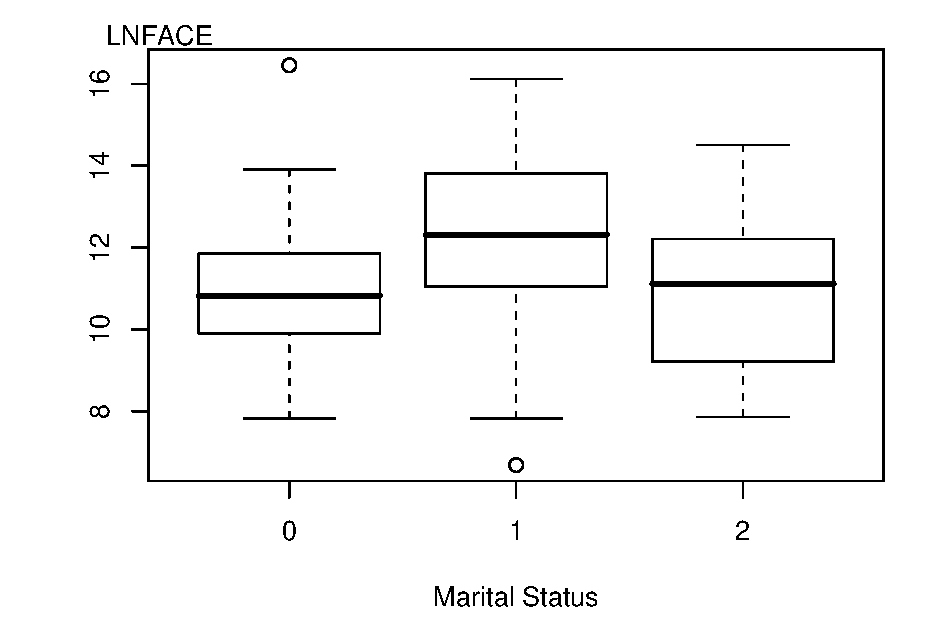
\includegraphics[width=.6\textwidth]{Chapter4/F4BoxFACEMARSTAT.eps}
       \caption{\label{F4:BoxFACEMARSTAT} \small  Box Plots of Logarithmic Face, by Level of Marital Status}
  \end{center}
\end{figure}

Are the continuous and categorical variables jointly important
determinants of response? To answer this, a regression was run using
LNFACE as the response and five explanatory variables, three
continuous and two binary (for marital status). Recall that our
three continuous explanatory variables are:  LNINCOME (logarithmic
annual income), the number of years of EDUCATION of the survey
respondent and the number of household members, NUMHH.

For the binary variables, first define MAR0 to be the binary
variable that is one if MARSTAT=0 and zero otherwise. Similarly,
define MAR1 and MAR2 to be binary variables that indicate MARSTAT=1
and MARSTAT=2, respectively. There is a perfect linear dependency
among these three binary variables in that MAR0 + MAR1 + MAR2 = 1
for any survey respondent. Thus, we need only two of the three.
However, there is \emph{not} a perfect dependency among any two of
the three. It turns out that Corr(MAR0,MAR1) = -0.90,
Corr(MAR0,MAR2) =-0.10 and Corr(MAR1,MAR2) = -0.34.

A regression model was run using LNINCOME, EDUCATION, NUMHH, MAR0
and MAR2 as explanatory variables. The fitted regression equation
turns out to be
\begin{eqnarray*}
\widehat{y} &=& 2.605 + 0.452 \textrm{LNINCOME} +0.205
\textrm{EDUCATION} + 0.248 \textrm{NUMHH} \\
 & & ~~ -0.557 \textrm{MAR0} -0.789 \textrm{MAR2}.
\end{eqnarray*}
To interpret the regression coefficients associated with marital
status, consider a respondent who is married. In this case, then
MAR0=0, MAR1=1 and MAR2=0, so that
\begin{eqnarray*}
\widehat{y}_m &=& 2.605 + 0.452 \textrm{LNINCOME} +0.205
\textrm{EDUCATION} + 0.248 \textrm{NUMHH} .
\end{eqnarray*}
Similarly, if the respondent is coded as living together, then
MAR0=0, MAR1=0 and MAR2=1, and
   \begin{eqnarray*}
\widehat{y}_{lt} &=& 2.605 + 0.452 \textrm{LNINCOME} +0.205
\textrm{EDUCATION} + 0.248 \textrm{NUMHH} -0.789.
\end{eqnarray*}
The difference between $\widehat{y}_m$ and $\widehat{y}_{lt}$ is
$0.789.$ Thus, we may interpret the regression coefficient
associated with MAR2, -0.789, to be the difference in fitted values
for someone living together compared to a similar person who is
married (the omitted category).

Similarly, we can interpret -0.557 to be the difference between the
``other'' category and the married category, holding other
explanatory variables fixed. For the difference in fitted values
between the ``other'' and the ``living together'' categories, we may
use $-0.557 - (-0.789) = 0.232.$

Although the regression was run using MAR0 and MAR2, any two out of
the three would produce the same ANOVA Table
\ref{T4:MSTermLifeANOVA}. However, the choice of binary variables
does impact the regression coefficients. Table
\ref{T4:MSTermLifeRegrCoeff} shows three models, omitting MAR1, MAR2
and MAR0, respectively. For each fit, the coefficients associated
with the continuous variables remain the same. As we have seen, the
binary variable interpretations are with respect to the omitted
category, known as the \emph{reference level}. Although they change
from model to model, they overall interpretation remains the same.
That is, if we would like to estimate the difference in coverage
between the ``other'' and the ``living together'' category, the
estimate would be 0.232, regardless of the model.

\index{categorical variable!reference level}

\begin{table}[h]
\scalefont{0.9} \caption{\label{T4:MSTermLifeANOVA} Term Life with
Marital Status ANOVA Table}
\begin{tabular}{lrrr}
 \hline Source
& Sum of Squares & $df$ & Mean Square \\ \hline

Regression & 343.28 & 5 &   68.66 \\
Error      & 615.62 & 269 &  2.29 \\
Total      & 948.90& 274 &   \\ \hline
\end{tabular}

Residual standard error $s= 1.513$, $R^2 = 35.8\%$, $R_a^2 = 34.6\%$
\scalefont{1.1111}
\end{table}


Although the three models in Table \ref{T4:MSTermLifeRegrCoeff} are
the same except for different choices of parameters, they do appear
different. In particular, the $t$-ratios differ and give different
appearances of statistical significance. For example, both of the
$t$-ratios associated with marital status in Model 2 are less than 2
in absolute value, suggesting that marital status is unimportant. In
contrast, both Models 1 and 3 have at least one marital status
binary that exceeds 2 in absolute value, suggesting statistical
significance. Thus, you can influence the \emph{appearance} of
statistical significance by altering the choice of the reference
level. To assess the overall importance of marital status (not just
each binary variable), Section \ref{S4:SeveralCoeff} will introduce
tests of sets of regression coefficients.


\marginparjed{The choice of the reference level can influence the
\textbf{appearance} of statistical significance.}

\begin{table}
\scalefont{0.9} \caption{\label{T4:MSTermLifeRegrCoeff} Term Life
Regression Coefficients with Marital Status}
\begin{tabular}{l|rr|rr|rr}
 \hline
 & \multicolumn{2}{c|}{Model 1}& \multicolumn{2}{c|}{Model 2}& \multicolumn{2}{c}{Model 3}\\
 \hline
 Explanatory \\
 Variable & Coefficient & $t$-ratio & Coefficient & $t$-ratio& Coefficient &
 $t$-ratio\\\hline
LNINCOME & 0.452 & 5.74 & 0.452 & 5.74 & 0.452 & 5.74 \\
EDUCATION &0.205 & 5.30 &0.205 & 5.30&0.205 & 5.30 \\
NUMHH     & 0.248 & 3.57 & 0.248 & 3.57 & 0.248 & 3.57 \\\hline
Intercept & 3.395 & 3.77  & 2.605&  2.74 & 2.838 & 3.34\\
MAR0    & -0.557 & -2.15&  0.232 &  0.44\\
MAR1 & & & 0.789 & 1.59 & 0.557 & 2.15\\
MAR2 & -0.789 & -1.59 & & & -0.232 & -0.44\\
\hline
\end{tabular}
\scalefont{1.1111}
\end{table}

\linejed \index{examples!Rand health insurance
experiment}\index{actuarial \& financial terms and concepts!adverse
selection}

\textbf{Example: How does Cost-Sharing in Insurance Plans affect
Expenditures in Healthcare?} In one of many studies that resulted
from the Rand Health Insurance Experiment (HIE) introduced in
Section 1.5, Keeler and Rolph (1988) investigated the effects of
cost-sharing in insurance plans. For this study, 14 health insurance
plans were grouped by the co-insurance rate (the percentage paid as
out-of-pocket expenditures that varied by 0, 25, 50 and 95\%). One
of the 95\% plans limited annual out-of-pocket outpatient
expenditures to \$150 per person (\$450 per family), providing in
effect an individual outpatient deductible. This plan was analyzed
as a separate group so that there were $c=5$ categories of insurance
plans. In most insurance studies, individuals choose insurance plans
making it difficult to assess cost-sharing effects because of
adverse selection. Adverse selection can arise because individuals
in poor chronic health are more likely to choose plans with less
cost sharing, thus giving the appearance that less coverage leads to
greater expenditures. In the Rand HIE, individuals were randomly
assigned to plans, thus removing this potential source of bias.

Keeler and Rolph (1988) organized an individual's expenditures into
episodes of treatment; each episode contains spending associated
with a given bout of illness, chronic condition or procedure.
Episodes were classified as hospital, dental or outpatient; this
classification was based primarily on diagnoses, not by location of
services. Thus, for example, outpatient services preceding or
following a hospitalization, as well as related drugs and tests,
were included as part of a hospital episode.

For simplicity, here we report only results for hospital episodes.
Although families were randomly assigned to plans, Keeler and Rolph
(1988) used regression methods to control for participant attributes
and isolate the effects of plan cost-sharing. Table
\ref{T4:RandHIECoefficients} summarizes the regression coefficients,
based on a sample of $n=1,967$ episode expenditures. In this
regression, logarithmic expenditure was the dependent variable.

The cost-sharing categorical variable was decomposed into five
binary variables so that no functional form was imposed on the
response to insurance. These variables are ``Co-ins25,''
``Co-ins50,'' and ``Co-ins95,'' for coinsurance rates 25, 50 and
95\%, respectively, and ``Indiv Deductible'' for the plan with
individual deductibles. The omitted variable is the free insurance
plan with 0\% coinsurance. The HIE was conducted in six cities; a
categorical variable to control for the location was represented
with five binary variables, Dayton, Fitchburg, Franklin, Charleston
and Georgetown, with Seattle being the omitted variable. A
categorical factor with $c=6$ levels was used for age and sex;
binary variables in the model consisted of ``Age 0-2,'' ``Age 3-5,''
``Age 6-17,'' ``Woman age 18-65,'' and ``Man age 46-65,'' the
omitted category was ``Man age 18-45.'' Other control variables
included a health status scale, socioeconomic status, number of
medical visits in the year prior to the experiment on a logarithmic
scale and race.

Table \ref{T4:RandHIECoefficients} summarizes the effects of the
variables. As noted by Keeler and Rolph, there were large
differences by site and age although the regression only served to
summarize $R^2=11\%$ of the variability. For the cost-sharing
variables, only ``Co-ins95'' was statistically significant, and this
only at the 5\% level, not the 1\% level.

The paper of Keeler and Rolph (1988) examines other types of episode
expenditures, as well as the frequency of expenditures. They
conclude that cost-sharing of health insurance plans has little
effect on the amount of expenditures per episode although there are
important differences in the frequency of episodes. This is because
an episode of treatment is composed of two decisions. The amount of
treatment is made jointly between the patient and the physician and
is largely unaffected by the type of health insurance plan. The
decision to seek health care treatment is made by the patient; this
decision-making process is more susceptible to economic incentives
in cost-sharing aspects of health insurance plans.


\begin{table}[h]
\caption{\label{T4:RandHIECoefficients} Coefficients of Episode
Expenditures from the Rand HIE}
\begin{tabular}{lr|lr}
   \hline
  Variable & Regression &   Variable & Regression \\
           & Coefficient &           & Coefficient \\
\hline
    Intercept &       7.95~ &            &            \\
    Dayton &       0.13* &    Co-ins25 &       0.07~~ \\
 Fitchburg &       0.12~ &    Co-ins50 &       0.02~~ \\
  Franklin &      -0.01~ &    Co-ins95 &      -0.13*~ \\
Charleston &       0.20* &    Indiv Deductible &      -0.03~~ \\
Georgetown &      -0.18* &            &            \\
           &            &            &            \\
Health scale &     -0.02* &    Age 0-2 &      -0.63** \\
Socioeconomic status &  0.03~ &    Age 3-5 &      -0.64** \\
Medical visits &      -0.03~ &   Age 6-17 &      -0.30** \\
Examination &      -0.10* & Woman age 18-65 &       0.11~~ \\
     Black &       0.14* & Man age 46-65 &       0.26~~ \\
 \hline
\multicolumn{4}{l}{Note: * significant at 5\%, ** significant at 1\%} \\
     \multicolumn{4}{l}{\textit{Source}: Keeler and Rolph (1988)} \\
      \hline
\end{tabular}
\end{table}

\linejed

\section{Statistical Inference for Several
Coefficients}\label{S4:SeveralCoeff}

It can be useful to examine several regression coefficients at the
same time. For example, when assessing the effect of a categorical
variable with $c$ levels, we need to say something jointly about the
$c-1$ binary variables that enter the regression equation. To do
this, Section \ref{S4:SetsRegCoeff} introduces a method for handling
linear combinations of regression coefficients. Section
\ref{S4:GenLinHypo} shows how to test several linear combinations
and Section \ref{S4:SetsInference} presents other inference
applications.


\subsection{Sets of Regression Coefficients}\label{S4:SetsRegCoeff}
\index{symbols!$\boldsymbol \beta$, vector of regression
coefficients}

Recall that our regression coefficients are specified by
$\boldsymbol \beta =\left( \beta_0, \beta_1, \ldots,\beta_k \right)
^{\prime},$ a $(k+1)\times 1$ vector. It will be convenient to
express linear combinations of the regression coefficients using the
notation $\mathbf{C} \boldsymbol \beta,$ where \textbf{C} is a
$p\times (k+1)$ matrix that is user-specified  and depends on the
application. Some applications involve estimating $\mathbf{C}
\boldsymbol \beta$. Others involve testing whether $\mathbf{C}
\boldsymbol \beta$ equals a specific known value (denoted as
\textbf{d}). We call $H_0:\mathbf{C \boldsymbol \beta =d}$ the
\emph{general linear hypothesis}. To demonstrate the broad variety
of applications in which sets of regression coefficients can be
used, we now present a series of special cases.\index{hypothesis
test!general linear hypothesis}

\marginparjed{The general \newline linear hypothesis is denoted as
\newline $H_0:\mathbf{C \boldsymbol \beta =d}$. }

\textbf{Special Case 1: One Regression Coefficient}. In Section 3.4,
we investigated the importance of a single coefficient, say
$\beta_j.$ We may express this coefficient as $\mathbf{C}
\boldsymbol \beta$ by choosing $p=1$ and \textbf{C} to be a $1\times
(k+1$) vector with a one in the $(j+1)st$ column and zeros
otherwise. These choices result in
\begin{equation*}
\mathbf{C \boldsymbol \beta =}\left( 0~\ldots~0~1~0~\ldots~0\right)
\left(
\begin{array}{c}
\beta_0 \\
\vdots  \\
\beta_k%
\end{array}
\right) =\beta_j.
\end{equation*}

\textbf{Special Case 2: Regression Function}. Here, we choose $p=1$
and \textbf{C} to be a $1\times (k+1$) vector representing the
transpose of a set of explanatory variables. These choices result in

\begin{equation*}
\mathbf{C \boldsymbol \beta =}\left(x_0,x_1, \ldots, x_k \right)
\left(
\begin{array}{c}
\beta_0 \\
\vdots  \\
\beta_k
\end{array}
\right) = \beta_0 x_0 + \beta_1 x_1 +\ldots + \beta_k x_k =
\mathrm{E} ~y,
\end{equation*}
the regression function.

\textbf{Special Case 3: Linear Combination of Regression
Coefficients}. When $p=1$, we use the convention that lower-case
bold letters are vectors and let $\mathbf{C = c^{\prime}}=
\left(c_0, \ldots, c_k \right)^{\prime}$. In this case, $\mathbf{C}
\boldsymbol \beta$ is a generic linear combination of regression
coefficients

\begin{equation*}
\mathbf{C} \boldsymbol \beta =\mathbf{c}^{\prime} \boldsymbol \beta
= c_0 \beta_0 + \ldots + c_k \beta_k.
\end{equation*}

\bigskip

\textbf{Special Case 4: Testing Equality of Regression
Coefficients}. Suppose that the interest is in testing $H_0: \beta_1
= \beta_2.$ For this purpose, let $p=1$, $\mathbf{c}^{\prime}=
\left(0,1, -1, 0, \ldots, 0\right),$ and \textbf{d}=0. With these
choices, we have

\begin{equation*}
\mathbf{C \boldsymbol \beta = c^{\prime} \boldsymbol \beta}=
\left(0,1, -1, 0, \ldots, 0\right) \left(
\begin{array}{c}
\beta_0 \\
\vdots  \\
\beta_k
\end{array}
\right) =\beta_1 - \beta_2 = 0,
\end{equation*}

\noindent so that the general linear hypothesis reduces to $H_0:
\beta_1 = \beta_2.$


\textbf{Special Case 5: Adequacy of the Model}. It is customary in
regression analysis to present a test of whether or not \emph{any}
of the explanatory variables are useful for explaining the response.
Formally, this is a test of the null hypothesis $H_0:\beta
_1=\beta_2=\ldots=\beta_k=0$. Note that, as a convention, one does
not test whether or not the intercept
is zero. To test this using the general linear hypothesis, we choose $p=k$, $%
\mathbf{d=}\left( 0~\ldots~0\right) ^{\prime}$ to be a $k\times 1$
vector of zeros and $\mathbf{C}$ to be a $k\times (k+1)$ matrix such
that
\begin{equation*}
\mathbf{C \boldsymbol \beta =}\left(
\begin{array}{ccccc}
0 & 1 & 0 & \cdots  & 0 \\
0 & 0 & 1 & \cdots  & 0 \\
\vdots  & \vdots  & \vdots  & \ddots  & \vdots  \\
0 & 0 & 0 & \cdots  & 1%
\end{array}%
\right) \left(
\begin{array}{c}
\beta_0 \\
\vdots  \\
\beta_k%
\end{array}%
\right) =\left(
\begin{array}{c}
\beta_1 \\
\vdots  \\
\beta_k%
\end{array}%
\right)  =\left(
\begin{array}{c}
0 \\
\vdots  \\
0
\end{array}%
\right) =\mathbf{d}.
\end{equation*}


\textbf{Special Case 6: Testing Portions of the Model.} Suppose that
we are interested in comparing a \emph{full} regression function

\begin{equation*}
\mathrm{E~}y = \beta_0 + \beta_1 x_1 +\ldots + \beta_k x_k + \beta
_{k+1} x_{k+1} + \ldots + \beta_{k+p} x_{k+p}
\end{equation*}
to a \emph{reduced} regression function,
\begin{equation*}
\mathrm{E~}y = \beta_0 + \beta_1 x_1 + \ldots + \beta_k x_k.
\end{equation*}
Beginning with the full regression, we see that if the null
hypothesis $H_0:\beta_{k+1} = \ldots = \beta_{k+p} = 0$ holds, then
we arrive at the reduced regression. To illustrate, the variables
$x_{k+1}, \ldots, x_{k+p}$ may refer to several binary variables
representing a categorial variable and our interest is in whether
the categorial variable is important. To test the importance of the
categorical variable, we want to see whether the binary variables
$x_{k+1}, \ldots, x_{k+p}$ \emph{jointly} affect the dependent
variables.

To test this using the general linear hypothesis, we choose
$\mathbf{d}$ and $\mathbf{C}$ such that
\begin{equation*}
\mathbf{C\boldsymbol \beta =}\left(
\begin{array}{ccccccc}
0 & \cdots  & 0 & 1 & 0 & \cdots  & 0 \\
0 & \cdots  & 0 & 0 & 1 & \cdots  & 0 \\
\vdots  & \vdots  & \vdots  & \vdots  & \vdots  & \ddots  & \vdots  \\
0 & \cdots  & 0 & 0 & 0 & \cdots  & 1%
\end{array}%
\right) \left(
\begin{array}{c}
\beta_0 \\
\vdots  \\
\beta_k \\
\beta_{k+1} \\
\vdots  \\
\beta_{k+p}%
\end{array}%
\right) =\left(
\begin{array}{c}
\beta_{k+1} \\
\vdots  \\
\beta_{k+p}%
\end{array}%
\right) =\left(
\begin{array}{c}
0 \\
\vdots  \\
0
\end{array}%
\right) =\mathbf{d}.
\end{equation*}
From a list of $k+p$ variables $x_1, \ldots, x_{k+p}$, you may drop
any $p$ that you deem appropriate. The additional variables do not
need to be the last $p$ in the regression specification. Dropping
$x_{k+1}, \ldots, x_{k+p}$ is for notational convenience only.


\subsection{The General Linear Hypothesis}\label{S4:GenLinHypo}

To recap, the general linear hypothesis can be stated as
$H_0:\mathbf{C \boldsymbol \beta =d}$. Here, $\mathbf{C}$ is a $p
\times (k+1)$ matrix, $\mathbf{d}$ is a $p \times 1$ vector and both
$\mathbf{C}$ and $\mathbf{d}$ are user specified and depend on the
application at hand. Although $k+1$ is the number of regression
coefficients, $p$ is the number of restrictions under $H_0$ on these
coefficients. (For those readers with knowledge of advanced matrix
algebra, $p$ is the rank of $\mathbf{C}$.) This null hypothesis is
tested against the alternative $H_a:\mathbf{C \boldsymbol \beta \neq
d}$. This may be obvious, but we do require $p \leq k+1$ because we
cannot test more constraints than free parameters.

To understand the basis for the testing procedure, we first recall
some of the basic properties of the regression coefficient
estimators described in Section 3.3. Now, however, our goal is to
understand properties of the linear combinations of regression
coefficients specified by $\mathbf{C\boldsymbol \beta } $. A natural
estimator of this quantity is $\mathbf{Cb}$. It is easy to see that
$\mathbf{Cb}$ is an unbiased estimator of $\mathbf{C\boldsymbol
\beta }$, because $
\mathrm{E~}\mathbf{Cb=C}\mathrm{E~}\mathbf{b=C\boldsymbol \beta }$.
Moreover, the
variance is $\mathrm{Var}\left( \mathbf{Cb}\right) \mathbf{=C}\mathrm{Var}%
\left( \mathbf{b}\right) \mathbf{C}^{\prime}=\sigma
^2\mathbf{C}\left( \mathbf{X^{\prime}X}\right)
^{-1}\mathbf{C}^{\prime}$. To assess the difference between
$\mathbf{d}$, the hypothesized value of $\mathbf{C \boldsymbol \beta
}$, and its estimated value, $\mathbf{Cb}$, we use the following
statistic
\begin{equation}\label{E4:GenLinHypF-ratio}
F-\textrm{ratio}=\frac{(\mathbf{Cb-d)}^{\prime}\left(
\mathbf{C}\left( \mathbf{X^{\prime}X} \right)
^{-1}\mathbf{C}^{\prime}\right) ^{-1}(\mathbf{Cb-d)}}{ps_{full}^2}.
\end{equation}
Here, $s_{full}^2$ is the mean square error from the full regression
model. Using the theory of linear models, it can be checked that the
statistic $F$-ratio has an $F$-distribution with numerator degrees
of freedom $df_1=p$ and denominator degrees of freedom
$df_2=n-(k+1)$. Both the statistic and the theoretical distribution
are named for R. A. Fisher, a renowned scientist and statistician
who did much to advance statistics as a science in the early half of
the twentieth century.\index{distributions!F-@{$F-$}}

Like the normal and the $t$-distribution, the $F$-distribution is a
continuous distribution. The $F$-distribution is the sampling
distribution for the $F$-ratio and is proportional to the ratio of
two sum of squares, each of which is positive or zero. Thus, unlike
the normal distribution and the $t$-distribution, the
$F$-distribution takes on only nonnegative values. Recall that the
$t$-distribution is indexed by a single degree of freedom parameter.
The $F$-distribution is indexed by two degree of freedom
parameters: one for the numerator, $df_1$, and one for the denominator, $%
df_2$. Appendix A3.4 provides additional details.

\marginparjed{Appendix A3.4 provides additional details about the
$F$-distribution, including a graph and distribution table.}

The test statistic in equation (\ref{E4:GenLinHypF-ratio}) is
complex in form. Fortunately, there is an alternative that is
simpler to implement and to interpret; this alternative is based on
the \emph{extra sum of squares principle}.\index{hypothesis
test!extra sum of squares principle}

\bigskip

\newpage

\boxedjed

\textit{Procedure for Testing the General Linear Hypothesis}

\begin{enumerate}
\item Run the full regression and get the error sum of squares and mean
square error, which we label as $(Error~SS)_{full}$ and
$s_{full}^2$, respectively.

\item Consider the model assuming the null hypothesis is true. Run a
regression with this model and get the error sum of squares, which we label $%
(Error~SS)_{reduced}$.

\item Calculate
\begin{equation}\label{E4:FratioErrSumSquares}
F-\textrm{ratio}=\frac{(Error~SS)_{reduced}-(Error~SS)_{full}}{ps_{full}^2}.
\end{equation}

\item Reject the null hypothesis in favor of the alternative if the $F$
-ratio exceeds an $F$-value. The $F$-value is a percentile from the
$F$-distribution with $df_1=p$ and $df_2=n-(k+1)$ degrees of
freedom. The percentile is one minus the significance level of the
test. Following our notation with the $t$-distribution, we denote
this percentile as $F_{p,n-(k+1),1-\alpha }$, where $\alpha$ is the
significance level.
\end{enumerate}
\end{boxedminipage}

\bigskip

\noindent This procedure is commonly known as an
$F$-test.\index{hypothesis test!$F$-test}

Section \ref{S4:MatrixSuccess} provides the mathematical
underpinnings. To understand the extra sum of squares principle,
recall that the error sum of squares for the full model is
determined to be the minimum value of
\begin{equation*}
SS(b_0^{\ast}, \ldots, b_k^{\ast}) = \sum_{i=1}^{n} \left( y_i -
\left( b_0^{\ast} + \ldots + b_k^{\ast} x_{i,k} \right) \right)^2.
\end{equation*}

\noindent Here, $SS(b_0^{\ast}, \ldots, b_k^{\ast})$ is a function
of $b_0^{\ast}, \ldots, b_k^{\ast}$ and $(Error~SS)_{full}$ is the
minimum over all possible values of $b_0^{\ast},\ldots,b_k^{\ast}$.
Similarly, $(Error~SS)_{reduced}$ is the minimum error sum of
squares under the constraints in the null hypothesis. Because there
are fewer possibilities under the null hypothesis, we have that

\begin{equation}\label{E4:DropErrorSS}
(Error~SS)_{full}\leq (Error~SS)_{reduced}.
\end{equation}


\marginparjed{When adding variables to a regression model, the error
sum of squares never goes up. The $R^2$ statistic never goes down.}

To illustrate, consider our first special case where $H_0 : \beta_j
= 0$. In this case, the difference between the full and reduced
models amounts to dropping a variable. A consequence of equation
(\ref{E4:DropErrorSS}) is that, when adding variables to a
regression model, the error sum of squares never goes up (and, in
fact, usually goes down). Thus, adding variables to a regression
model increases $R^2,$ the coefficient of determination.

How large a decrease in the error sum of squares is statistically
significant? Intuitively, one can view the $F$-ratio as the
difference in the error sum of squares divided by the number of
constraints, $((Error~SS)_{reduced}-(Error~SS)_{full})/p,$ and then
rescaled by the best estimate of the variance term, the $s^2,$ from
the full model. Under the null hypothesis, this statistic follows an
$F$-distribution and we may compare the test statistic to this
distribution to see if it is unusually large.

Using the relationship $Regression~SS=Total~SS-Error~SS$, we can
re-express the difference in the error sum of squares as
\scalefont{0.9}
\begin{equation*}
(Error~SS)_{reduced}-(Error~SS)_{full}=(Regression~SS)_{full}-(Regression~SS)_{reduced}.
\end{equation*} \scalefont{1.1111}
This difference is known as a \emph{Type III Sum of Squares}. When
testing the importance of a set of explanatory variables,
$x_{k+1},\ldots,x_{k+p},$ in the presence of $x_1,\ldots,x_k$, you
will find that many statistical software packages compute this
quantity directly in a single regression run. The advantage of this
is it allows the analyst to perform an $F$-test using a single
regression run, instead of two regression runs as in our four-step
procedure described above.

\linejed \index{datasets!term life insurance}

\textbf{Example: Term Life Insurance - Continued.} Before discussing
the logic and the implications of the $F$-test, let us illustrate
the use of it. In the Term Life Insurance example, suppose that we
wish to understand the impact of marital status. Table
\ref{T4:MSTermLifeRegrCoeff} presented a mixed message in terms of
$t$-ratios, sometimes they were statistically significant and
sometimes not. It would be helpful to have a formal test to give a
definitive answer, at least in terms of statistical significance.
Specifically, we consider a regression model using LNINCOME,
EDUCATION, NUMHH, MAR0 and MAR2 as explanatory variables. The model
equation is
\begin{eqnarray*}
y &=& \beta_0 + \beta_1 \textrm{LNINCOME} +\beta_2
\textrm{EDUCATION} + \beta_3 \textrm{NUMHH} \\
 & & ~~ +\beta_4 \textrm{MAR0} +\beta_5\textrm{MAR2}.
\end{eqnarray*}
Our goal is to test $H_0: \beta_4 = \beta_5 = 0 $.

\begin{enumerate}
\item We begin by running a regression model
with all $k+p=5$ variables. The results were reported in Table
\ref{T4:MSTermLifeANOVA} where we saw that $(Error~SS)_{full} =
615.62$ and $s_{full}^2 = (1.513)^2 = 2.289$.

\item The next step is to run the reduced model without MAR0 and MAR2.
This was done in Table 3.3 of Chapter 3, where we saw that
$(Error~SS)_{reduced} = 630.43.$

\item We then calculate the test statistic
\begin{equation*}
F-\textrm{ratio}=\frac{(Error~SS)_{reduced}-(Error~SS)_{full}}{ps_{full}^2}
= \frac{630.43 -615.62}{2 \times 2.289} = 3.235 .
\end{equation*}

\item The fourth step compares the test statistic to an $F$-distribution with
$df_1=p=2$ and $df_2 = n-(k+p+1) = 269$ degrees of freedom. Using a
5\% level of significance, it turns out that the 95$th$ percentile
is $F-\textrm{value} \approx 3.029$. The corresponding $p$-value is
$\Pr(F > 3.235) = 0.0409$. At the 5\% significance level, we reject
the null hypothesis $H_0:\beta_4=\beta_5=0$. This suggests that it
is important to use marital status to understand term life insurance
coverage, even in the presence of income, education and number of
household members.

\end{enumerate}

\linejed

\subsubsection*{Some Special Cases}

The general linear hypothesis test is available when you can express
one model as a subset of another. For this reason, it useful to
think of it as a device for comparing ``smaller'' to ``larger''
models. However, the smaller model must be a subset of the larger
model. For example, the general linear hypothesis test cannot be
used to compare the regression functions $\mathrm{ E~}y = \beta_0 +
\beta_7 x_7$ versus $\mathrm{E~}y = \beta_0 + \beta_1 x_1 + \beta_2
x_2 + \beta_3 x_3 + \beta_4 x_4$. This is because the former,
smaller function is not a subset of the latter, larger function.

The general linear hypothesis can be used in many instances,
although its use is not always necessary. For example, suppose that
we wish to test $H_0:\beta_k=0$. We have already seen that this null
hypothesis can be examined using the $t$-ratio test. In this special
case, it turns out that $(t-\textrm{ratio})^2=F-\textrm{ratio}$.
Thus, these tests are equivalent for testing $H_0:\beta_k=0$ versus
$H_a:\beta_k \neq 0$. The $F$-test has the advantage that it works
for more than one predictor whereas the $t$-test has the advantage
that one can consider one-sided alternatives. Thus, both tests are
considered useful.

Dividing the numerator and denominator of equation (\ref
{E4:FratioErrSumSquares}) by $Total~SS$, the test statistic can also
be written as:
\begin{equation}\label{E4:FratioRsquare}
F-\textrm{ratio}=\frac{\left( R_{full}^2-R_{reduced}^2\right)
/p}{\left( 1-R_{full}^2\right) /(n-(k+1))}.
\end{equation}
The interpretation of this expression is that the $F$-ratio measures
the drop in the coefficient of determination, $R^2$.

The expression in equation (\ref{E4:FratioErrSumSquares}) is
particularly useful for testing the adequacy of the model, our
Special Case 5. In this case, $p=k$, and the regression sum of
squares under the reduced model is zero. Thus, we have
\begin{equation*}
F-\textrm{ratio}=\frac{\left( (Regression~SS)_{full}\right) /k}{s_{full}^2}=\frac{%
(Regression~MS)_{full}}{(Error~SS)_{full}}.
\end{equation*}
This test statistic is a regular feature of the ANOVA table for many
statistical packages.

For example, in our Term Life Insurance example, testing the
adequacy of the model means evaluating $H_0: \beta_1 = \beta_2
=\beta_3 =\beta_4 =\beta_5 = 0$. From Table
\ref{T4:MSTermLifeANOVA}, the $F$-ratio is 68.66 / 2.29 = 29.98.
With $df_1=5$ and $df_2 = 269$, we have that the $F$-value is
approximately 2.248 and the corresponding $p$-value is $\Pr(F >
29.98) \approx 0$. This leads us to reject strongly the notion that
the explanatory variables are not useful in understanding term life
insurance coverage, reaffirming what we learned in the graphical and
correlation analysis. Any other result would be surprising.

For another expression, dividing by $Total~SS$, we may write
\begin{equation*}
F-\textrm{ratio}=\frac{R^2}{1-R^2}\frac{n-(k+1)}{k}.
\end{equation*}%
Because both $F$-ratio and $R^2$ are measures of model fit, it seems
intuitively plausible that they be related in some fashion. A
consequence of this relationship is the fact that as $R^2$
increases, so does the $F$-ratio and vice versa. The $F$-ratio is
used because its sampling distribution is known under a null
hypothesis so we can make statements about statistical significance.
The $R^2$ measure is used because of the easy interpretations
associated with it.

\subsection{Estimating and Predicting Several Coefficients}\label{S4:SetsInference}

\subsubsection*{Estimating Linear Combinations of Regression Coefficients}

In some applications, the main interest is to estimate a linear
combination of regression coefficients. To illustrate, recall in
Section 3.5 that we developed a regression function for an
individual's charitable contributions ($y$) in terms of their wages
($x$). In this function, there was an abrupt change in the function
at $x=97,500$. To model this, we defined the binary variable $z$ to
be zero if $x<97,500$ and to be one if $x\geq 97,500$ and the
regression function $\mathrm{E~}y=\beta_0+\beta_1x+\beta
_2z(x-97,500)$. Thus, the marginal expected change in contributions
per dollar wage change for wages in excess of 97,500 is $\partial
\left( \mathrm{E~}y\right) /\partial x=\beta_1+\beta _2$.

To estimate $\beta_1+\beta_2$, a reasonable estimator is $b_1+b_2$
which is readily available from standard regression software. In
addition, we would also like to compute standard errors for
$b_1+b_2$ to be used, for example, in determining a confidence
interval for $\beta_1+\beta_2$. However, $b_1$ and $b_2$ are
typically correlated so that the calculation of the standard error
of $b_1+b_2$ requires estimation of the covariance between $b_1$ and
$b_2$.

Estimating $\beta_1 + \beta_2$ is an example of our Special Case 3
that considers linear combinations of regression coefficients of the
form $\mathbf{c}^{\prime}  \boldsymbol \beta=c_0\beta
_0+c_1\beta_1+\ldots+c_k\beta_k$. For our charitable contribution's
example, we would choose $c_1=c_2=1$ and other $c$'s equal to zero.

To estimate $\mathbf{c}^{\prime} \boldsymbol \beta $, we replace the
vector of
parameters by the vector of estimators and use $\mathbf{c}^{\prime}\mathbf{b%
}$. To assess the reliability of this estimator, as in Section
4.2.2, we have that $\mathrm{Var}\left(
\mathbf{c}^{\prime}\mathbf{b}\right) =\sigma^2
\mathbf{c}^{\prime}(\mathbf{X^{\prime}X)}^{-1}\mathbf{c}$. Thus, we
may define the estimated standard deviation, or standard error, of
$\mathbf{c} ^{\prime}\mathbf{b}$ to be
\begin{equation*}
se\left( \mathbf{c}^{\prime}\mathbf{b}\right) =s\sqrt{\mathbf{c}^{\prime}(%
\mathbf{X^{\prime}X)}^{-1}\mathbf{c}}.
\end{equation*}%
With this quantity, a $100(1-\alpha ) \%$ confidence interval for
$\mathbf{c}^{\prime} \boldsymbol \beta$ is
\begin{equation}  \label{E4:ConfIntLinCombination}
\mathbf{c}^{\prime}\mathbf{b}\pm t_{n-(k+1),1-\alpha /2} ~se(\mathbf{c}%
^{\prime}\mathbf{b}).
\end{equation}

The confidence interval in equation (\ref{E4:ConfIntLinCombination})
is valid under Assumptions F1-F5. If we choose $\mathbf{c}$ to have
a ``1'' in the $(j+1)st$ row and zeros otherwise, then
$\mathbf{c}^{\prime}\boldsymbol \beta =\beta _j$,
$\mathbf{c}^{\prime}\mathbf{b=}b_j$ and
\begin{equation*}
se(b_j)=s\sqrt{
(j+1)st~diagonal~element~of~(\mathbf{X^{\prime}X)}^{-1}}.
\end{equation*} Thus, (\ref{E4:ConfIntLinCombination}) provides a
theoretical basis for the individual regression coefficient
confidence intervals introduced in Section 3.4's equation (3.10) and
generalizes it to arbitrary linear combinations of regression
coefficients.

Another important application of equation
(\ref{E4:ConfIntLinCombination}) is the choice of $\mathbf{c}$
corresponding to a set of explanatory variables of interest, say,
$\mathbf{x}_{\ast}=\left( 1,x_{\ast 1},x_{\ast 2},\ldots,x_{\ast k}
\right)^{\prime}$. These may correspond to an observation within the
data set or to a point outside the available data. The parameter of
interest, $\mathbf{c}^{\prime} \boldsymbol \beta =
\mathbf{x}_{\ast}^{\prime} \boldsymbol \beta $, is the expected
response or the regression function at that point. Then,
$\mathbf{x}_{\ast}^{\prime} \mathbf{b}$ provides a point estimator
and equation (\ref{E4:ConfIntLinCombination}) provides the
corresponding confidence interval.

\subsubsection*{Prediction Intervals}

Prediction is an inferential goal that is closely related to
estimating the regression function at a point. Suppose that, when
considering charitable contributions, we know an individual's wages
(and thus whether wages are in excess of 97,500) and wish to predict
the amount of charitable contributions. In general, we assume that
the set of explanatory variables $\mathbf{x}_{\ast}$ is known and
wish to predict the corresponding response $y_{\ast}$. This new
response follows the assumptions as described in Section 3.2.
Specifically, the expected response is $\mathrm{E~}y_{\ast}=
\mathbf{x}_{\ast}^{\prime} \boldsymbol \beta $, $\mathbf{x}_{\ast}$
is nonstochastic, $\mathrm{Var~}y_{\ast}=\sigma^2$, $y_{\ast}$ is
independent of $\{y_1,\ldots,y_{n}\}$ and is normally distributed.
Under these assumptions, a 100(1-$\alpha $)\% prediction interval
for $y_{\ast}$ is
\begin{equation}\label{E4:PredictionInterval}
\mathbf{x}_{\ast}^{\prime} \mathbf{b} \pm t_{n-(k+1),1-\alpha /2} ~s
\sqrt{1 + \mathbf{x}_{\ast}^{\prime} ( \mathbf{X}^{\prime}\mathbf{X}
)^{-1} \mathbf{x}_{\ast}}.
\end{equation}
Equation (\ref{E4:PredictionInterval}) generalizes the prediction
interval introduced in Section 2.4.


\section{One Factor ANOVA Model}\label{S4:OneFactor}

Section \ref{S4:BinaryVar} showed how to incorporate unordered
categorical variables, or factors, into a linear regression model
through the use of binary variables. Factors are important in social
science research; they can be used to classify people by gender,
ethnicity, marital status and so on, or classify firms by geographic
region, organizational structure and so forth. Within studies of
insurance, factors are used by insurers to categorize policyholders
according to a ``risk classification system.'' Here, the idea is to
create groups of policyholders with similar risk characteristics
that will have similar claims experience. These groups form the
basis of insurance pricing, so that each policyholder is
charged an amount that is appropriate to their risk category. This
process is sometimes known as ``segmentation.''

Although factors may be represented as binary variables in a linear
regression model, we study one factor models as a separate unit
because:
\begin{itemize}
\item The method of least squares is much simpler, obviating the need to take inverses of high dimensional matrices.
\item The resulting interpretations of coefficients are more straightforward.
\end{itemize}
The one factor model is still a special case of the linear
regression model. Hence, no additional statistical theory is needed
to establish its statistical inference capabilities.

To establish notation for the one factor ANOVA model, we now
consider the following example.

\linejed

\empexjed{AutoClaims} \index{datasets!automobile insurance
claims}\index{actuarial \& financial terms and concepts!closed
claim}

\textbf{Example: Automobile Insurance
Claims.}\ecaptionjed{Automobile Claims} We examine claims experience
from a large midwestern (US) property and casualty insurer for
private passenger automobile insurance. The dependent variable is
the amount paid on a closed claim, in (US) dollars (claims that were
not closed by year end are handled separately). Insurers categorize
policyholders according to a risk classification system. This
insurer's risk classification system is based on:
\begin{itemize}
\item Automobile operator characteristics (age, gender, marital
  status and whether the primary or occasional driver of a car).
\item Vehicle characteristics (city versus farm usage, if the vehicle is used to commute to school or
    work, used for business or pleasure, and if commuting, the
    approximate distance of the commute).
\end{itemize}
These factors are summarized by the risk class categorical variable
CLASS. Table \ref{T4:AutoSumStats} shows 18 risk classes - further
classification information is not given here to protect proprietary
interests of the insurer.

Table \ref{T4:AutoSumStats} summarizes the results from $n=6,773$
claims for drivers aged 50 and above. We can see the the median
claim varies from a low of \$707.40 (CLASS F7) to a high of
\$1,231.25 (CLASS C72). The distribution of claims turns out to be
skewed, so we consider $y$ = logarithmic claims. The table presents
means, medians and standard deviations. Because the distribution of
logarithmic claims is less skewed, means are close to medians.
Figure \ref{F4:BoxplotAuto} shows the distribution of logarithmic
claims by risk class.



\begin{table}[h]\scalefont{0.9}
\caption{\label{T4:AutoSumStats} Automobile Claims Summary
Statistics by Risk Class}
\begin{tabular}{l|rrrrrr}
\hline
     Class &        C1  &        C11 &        C1A &        C1B &        C1C &        C2  \\
    Number &        726 &       1,151 &         77 &        424 &         38 &         61 \\
Median (dollars) &     948.86 &   1,013.81 &     925.48 &   1,026.73 &   1,001.73 &     851.20 \\
Median (in log dollars) &      6.855 &      6.921 &      6.830 &      6.934 &      6.909 &      6.747 \\
Mean (in log dollars) &      6.941 &      6.952 &      6.866 &      6.998 &      6.786 &      6.801 \\
Std Dev (in log dollars) &      1.064 &      1.074 &      1.072 &      1.068 &      1.110 &      0.948 \\
\hline
     Class &        C6  &        C7  &        C71 &        C72 &        C7A &        C7B \\
    Number &        911 &        913 &       1,129 &         85 &        113 &        686 \\
Median (dollars) &   1,011.24 &     957.68 &     960.40 &   1,231.25 &   1,139.93 &   1,113.13 \\
Median (in log dollars) &      6.919 &      6.865 &      6.867 &      7.116 &      7.039 &      7.015 \\
Mean (in log dollars) &      6.926 &      6.901 &      6.954 &      7.183 &      7.064 &      7.072 \\
Std Dev (in log dollars) &      1.115 &      1.058 &      1.038 &      0.988 &      1.021 &      1.103 \\
\hline
     Class &        C7C &        F1  &        F11 &        F6  &        F7  &        F71 \\
    Number &         81 &         29 &         40 &        157 &         59 &         93 \\
Median (dollars) &   1,200.00 &   1,078.04 &     774.79 &   1,105.04 &     707.40 &   1,118.73 \\
Median (in log dollars) &      7.090 &      6.983 &      6.652 &      7.008 &      6.562 &      7.020 \\
Mean (in log dollars) &      7.244 &      7.004 &      6.804 &      6.910 &      6.577 &      6.935 \\
Std Dev (in log dollars) &      0.944 &      0.996 &      1.212 &
1.193 &      0.897 &      0.983 \\
\hline
\end{tabular}\scalefont{1.1111}
\end{table}

\begin{figure}[htp]
  \begin{center}
    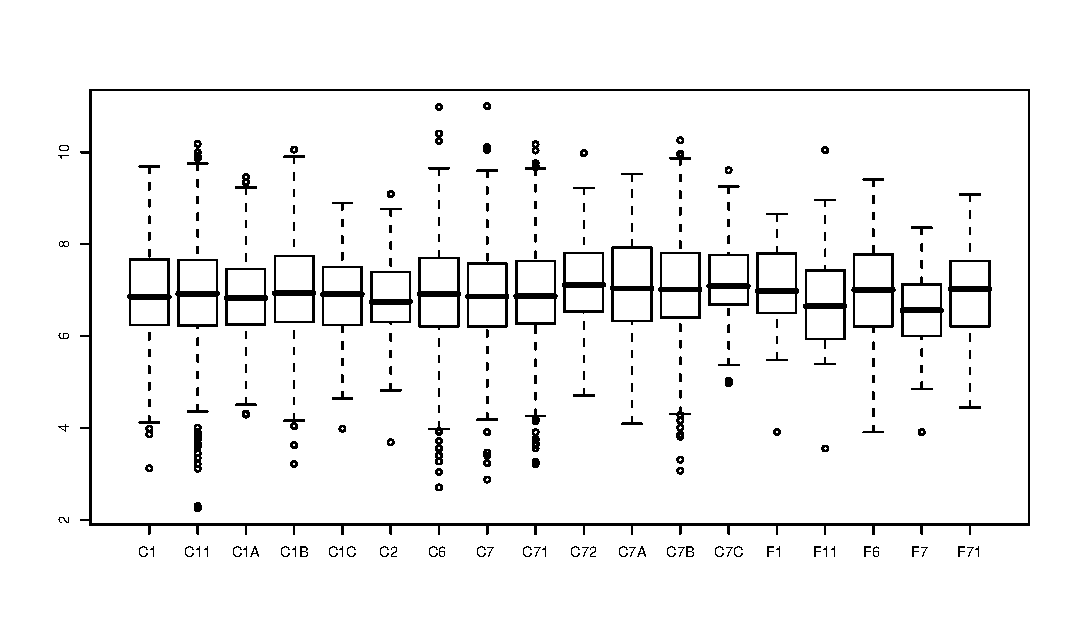
\includegraphics[width=1\textwidth]{Chapter4/Fig4BoxplotAuto.eps}
        \caption{\label{F4:BoxplotAuto} \small  Box Plots of Logarithmic Claims by Risk Class}
  \end{center}
\end{figure}

\linejed


This section focuses on the risk class (CLASS) as
the explanatory variable. We use the notation $y_{ij}$ to mean
the $i$th observation of the $j$th risk class. For the $j$th risk class, we assume
there are $n_j$ observations. There are $n=n_1+n_2+\ldots +n_c$
observations. The data are:

\begin{center}
\begin{tabular}{cccccc}
Data for risk class 1 & \ \ \ \ \ \ \ \ \ \ \ \ \ \ \  & $y_{11}$ & $y_{21}$ & $%
\ldots $ & $y_{n_1,1}$ \\
Data for risk class 2 &  & $y_{12}$ & $y_{22}$ & $\ldots $ & $y_{n_2,1}$ \\
. &  & $.$ & $.$ & $\ldots$ & $.$ \\
Data for risk class $c$ &  & $y_{1c}$ & $y_{2c}$ & $\ldots $ & $y_{n_c,c}$%
\end{tabular}
\end{center}

\noindent where $c=18$ is the number of levels of the CLASS factor.
Because each level of a factor can be arranged in a single row (or
column), another term for this type of data is a ``one way
classification.'' Thus, a \textit{one way model} is another term for
a one factor model.

An important summary measure of each level of the factor is the sample
average. Let
\begin{equation*}
\overline{y}_j=\frac{1}{n_j}\sum_{i=1}^{n_j}y_{ij}
\end{equation*}
denote the average from the $j$th CLASS.

\subsubsection*{Model Assumptions and Analysis}

The one factor ANOVA model equation is
\begin{equation}\label{E4:OneFactorEquation}
y_{ij}=\mu_j+ \varepsilon_{ij}\ \ \ \ \ \ i=1,\ldots ,n_j,\ \ \ \ \
j=1,\ldots ,c.
\end{equation}
As with regression models, the random deviations $\{
\varepsilon_{ij} \}$ are assumed to be zero mean with constant
variance (Assumption E3) and independent of one another (Assumption
E4). Because we assume the expected value of each deviation is zero,
we have E$\,y_{ij}=\mu_j$. Thus, we interpret $\mu_j$ to be the
expected value of the response $y_{ij}$, that is, the mean $\mu$
varies by the $j$th factor level.

To estimate the parameters $\{\mu_j\}$, as with regression we use
the \textit{method of least squares}, introduced in Section 2.1.
That is, let $\mu^{\ast}_j$ be a ``candidate'' estimate of $\mu_j$.
The quantity $ SS(\mu^{\ast}_1, \ldots , \mu^{\ast}_{c}) =
\sum_{j=1}^{c} \sum_{i=1}^{n_j} (y_{ij}-\mu^{\ast}_j)^2 $ represents
the sum of squared deviations of the responses from these candidate
estimates. From straight-forward algebra, the value of
$\mu^{\ast}_j$ that minimizes this sum of squares is $\bar{y}_j$.
Thus, $\bar{y}_j$ is the \textit{least squares estimate }of $\mu
_j$.

\marginparjed{The least squares estimate of $\mu _j$ is $\bar{y}_j$.}

To understand the reliability of the estimates, we can partition the
variability as in the regression case, presented in Sections 2.3.1
and 3.3. The minimum sum of squared deviations is called the
\textit{error sum of squares} and is defined to be

\begin{equation*}
Error~SS = SS(\bar{y}_1, \ldots, \bar{y}_{c}) = \sum_{j=1}^{c}
\sum_{i=1}^{n_j} \left(y_{ij}-\bar{y}_j \right)^2 .
\end{equation*}
The total variation in the data set is summarized by the
\textit{total sum of squares}, $Total~SS =
\sum_{j=1}^{c}\sum_{i=1}^{n_j}(y_{ij}-\bar{y})^2$ . The difference,
called the \textit{factor sum of} \textit{squares}, can be expressed
as:

\begin{eqnarray*}
Factor~SS &=& Total~SS -- Error~SS \\
&=& \sum_{j=1}^{c}\sum_{i=1}^{n_j}(y_{ij}-\bar{y})^2-\sum_{j=1}^{c}%
\sum_{i=1}^{n_j}(y_{ij}-\bar{y}_j)^2=\sum_{j=1}^{c}\sum_{i=1}^{n_j}(%
\bar{y}_j-\bar{y})^2 \\
&=& \sum_{j=1}^{c}n_j(\bar{y}_j-\bar{y})^2 .
\end{eqnarray*}
The last two equalities follow from algebra manipulation. The
$Factor~SS$ plays the same role as the $Regression~SS$ in Chapters 2
and 3. The variability decomposition is summarized in the following
analysis of variance (ANOVA) table.
\newpage
\begin{table}[h]
\caption{\label{T4:ANOVAOneFactor} ANOVA Table for One Factor Model}
\begin{tabular}{llcl}
\hline Source & Sum of Square & \textit{df} & Mean Square \\
\hline
Factor & $Factor~SS$ & $c-1$ & $Factor~MS$ \\
Error  & $Error~SS$  & $n-c$ & $Error~MS$ \\
Total  & $Total~SS$  & $n-1$ & \\
\hline
\end{tabular}
\end{table}

\noindent The conventions for this table are the same as in the
regression case. That is, the mean square (MS) column is defined by
the sum of squares (SS) column divided by the degrees of freedom
(\textit{df}) column. Thus, $Factor$ $MS\equiv (Factor$ $SS)/(c-1)$
and $Error$ $MS\equiv (Error$ $SS)/(n-c)$. We use
\begin{equation*}
s^2=Error~MS=\frac{1}{n-c} \sum_{j=1}^{c}\sum_{i=1}^{n_j} e_{ij}^2
\end{equation*}
to be our estimate of $\sigma^2$, where $e_{ij}=y_{ij}-\bar{y}_j$ is
the residual.

With this value for $s$, it can be shown that the interval estimate
for $\mu_j$ is
\begin{equation}\label{E4:OneFactorConInt}
\bar{y}_j \pm t_{n-c,1-\alpha /2}\frac{s}{\sqrt{n_j}}.
\end{equation}

\noindent Here, the \textit{t}-value $t_{n-c,1-\alpha /2}$ is a
percentile from the \textit{t}-distribution with $df=n-c$ degrees of
freedom.

\linejed \index{datasets!automobile insurance claims}

\textbf{Example: Automobile Claims - Continued.} To illustrate, the
ANOVA table summarizing the fit for the automobile claims data
appears in Table \ref{T4:ANOVAAuto}. Here, we see that the mean
square error is $s^2 = 1.14.$

\begin{table}[h]
\caption{\label{T4:ANOVAAuto} ANOVA Table for Logarithmic Automobile
Claims}
\begin{tabular}{lrrr}
\hline Source & Sum of Squares & \textit{df} & Mean Square \\
\hline
CLASS & 39.2 & 17 & 2.31\\
Error  & 7729.0 & 6755& 1.14\\
Total  & 7768.2  & 6772 & \\
\hline
\end{tabular}
\end{table}

In automobile ratemaking, one uses the average claims to help set
prices for insurance coverages. As an example, for CLASS C72 the
average logarithmic claim is 7.183. From equation
(\ref{E4:OneFactorConInt}), a 95\% confidence interval is
\begin{equation*}
7.183 \pm (1.96) \frac{\sqrt{1.14}}{\sqrt{85}} = 7.183 \pm 0.227 =
(6.952 ,7.410).\end{equation*} Note that these estimates are in
natural logarithmic units. In dollars, our point estimate is
$e^{7.183}$ = \$1,316.85 and our 95\% confidence interval is
($e^{6.952} ,e^{7.410}$), or (\$1,045.24, \$1,652.43).

\linejed

\newpage

\marginparjed{Unlike the usual regression analysis, no matrix
calculations are required for the one factor ANOVA decomposition and
estimation.}

An important feature of the one factor ANOVA decomposition and
estimation is the ease of computation. Although the sum of squares
appear complex, it is important to note that \emph{no matrix
calculations are required}. Rather, all of the calculations can be
done through averages and sums of squares. This been an important
consideration historically, before the age of readily available
desktop computing. Moreover, insurers may segment their portfolios
into hundreds or even thousands of risk classes instead of the 18
used in our Automobile Claims data. Thus, even today it can be
helpful to identify a categorical variable as a factor and let your
statistical software use ANOVA estimation techniques. Further, ANOVA
estimation also provides for direct interpretation of the results.


\subsubsection*{Link with Regression}

This subsection shows how a one factor ANOVA model can be rewritten
as a regression model. To this end, we have seen that both the
regression model and one factor ANOVA model use a linear error
structure with Assumptions E3 and E4 for identically and
independently distributed errors. Similarly, both use the normality
assumption E5 for selected inference results (such as confidence
intervals). Both employ non-stochastic explanatory variables as in
Assumption E2. Both have an additive (mean zero) error term, so the
main apparent difference is in the expected response, E $y$.

For the linear regression model, E $y$ is a linear combination of
explanatory variables (Assumption F1). For the one factor ANOVA
model, E $y_j = \mu_j$ is a mean that depends on the level of the
factor. To equate these two approaches, for the ANOVA factor with
$c$ levels, we define $c$ binary variables, $x_1,$ $x_2,\ldots
,x_c$. Here, $x_j$ indicates whether or not an observation falls in
the $j$th level. With these variables, we can rewrite our one factor
ANOVA model as
\begin{equation}\label{E4:OneFactor}
y = \mu_1 x_1 + \mu_2 x_2 + \ldots + \mu_c x_c + \varepsilon.
\end{equation}
Thus, we have re-written the one factor ANOVA expected response as a
regression function, although using a no-intercept form (as in
equation 3.5).

\marginparjed{The one factor ANOVA is a special case of the
regression model, using binary variables from the factor as
explanatory variables in the regression function.}

The one factor ANOVA is a special case of our usual regression
model, using binary variables from the factor as explanatory
variables in the regression function. As we have seen, no matrix
calculations are needed for least squares estimation. However, one
can always use the matrix procedures developed in Chapter 3. Section
\ref{S4:CatVarMatrix} shows how our usual matrix expression for
regression coefficients ($\mathbf{b} =
\left(\mathbf{X}^{\prime}\mathbf{X}
\right)^{-1}\mathbf{X}^{\prime}\mathbf{y}$) reduce to the simple
estimates $\bar{y}_j$ when using only one categorical variable.

\subsubsection*{Reparameterization}

To include an intercept term, define $\tau_j = \mu_j - \mu $, where
$\mu$ is an, as yet, unspecified parameter. Because each observation
must fall into one of the $c$ categories, we have $x_1+x_2+\ldots
+x_{c}=1$ for each observation. Thus, using $\mu _j = \tau_j + \mu $
in equation (\ref{E4:OneFactor}), we have
\begin{equation}\label{E4:OneFactorTau}
y=\mu +\tau_1x_1+\tau_2x_2+\ldots +\tau_{c}x_{c}+\varepsilon.
\end{equation}
Thus, we have re-written the model into what appears to be our usual
regression format.

We use the $\tau $ in lieu of $\beta $ for historical reasons. ANOVA
models were invented by R.A. Fisher in connection with agricultural
experiments. Here, the typical set-up is to apply several
\textit{treatments} to plots of land in order to quantify crop yield
responses. Thus, the Greek ``t", $\tau ,$ suggests the word
treatment, another term used to described levels of the factor of
interest.

A simpler version of equation (\ref{E4:OneFactorTau}) can be given
when we identify the factor level. That is, if we know an
observation falls in the $j$th level, then only $x_j$ is one and the
other $x$'s are 0. Thus, a simpler expression for equation
(\ref{E4:OneFactorTau}) is

\begin{equation*}
y_{ij}=\mu +\tau_j + \varepsilon_{ij}.
\end{equation*}

Comparing equations (\ref{E4:OneFactor}) and
(\ref{E4:OneFactorTau}), we see that the number of parameters
has increased by one. That is, in equation (\ref{E4:OneFactor}), there are $c$ parameters, $%
\mu_1,\ldots ,\mu_c$, even though in equation
(\ref{E4:OneFactorTau}) there are $c+1$ parameters, $\mu $ and $\tau
_1,\ldots ,\tau_c$. The model in equation (\ref{E4:OneFactorTau}) is
said to be \textit{overparameterized}. It is possible to estimate
this model directly, using the general theory of linear models,
summarized in Section \ref{S4:GeneralLinearModel}. In this theory,
regression coefficients need not be identifiable. Alternatively, one
can make these two expressions equivalent \textit{restricting} the
movement of the parameters in (\ref{E4:OneFactorTau}). We now
present two ways of imposing restrictions.

The first type of restriction, usually done in the regression context, is to
require one of the $\tau $'s to be zero. This amounts to \textit{dropping}
one of the explanatory variables. For example, we might use

\begin{equation}  \label{E4:OneFactorTauDrop}
y=\mu +\tau_1x_1+\tau_2x_2+\ldots +\tau _{c-1}x_{c-1}+\varepsilon,
\end{equation}
dropping $x_c$. With this formulation, it is easy to fit the model
in equation (\ref{E4:OneFactorTauDrop}) using regression statistical
software routines because one only needs to run the regression with
$c-1$ explanatory variables. However, one needs to be careful with
the interpretation of parameters. To equate the models in
(\ref{E4:OneFactor}) and (\ref{E4:OneFactorTau}), we need to define
$\mu \equiv \mu_c$ and $\tau_j=\mu_j-\mu_c$ for $j=1,2,\ldots ,c-1$.
That is, the regression intercept term is the mean level of the
category dropped, and each regression coefficient is the difference
between a mean level and the mean level dropped. It is not necessary
to drop the last level c, and indeed, one could drop any level.
However, the interpretation of the parameters does depend on the
variable dropped. With this restriction, the fitted values are
$\hat{\mu}=\hat{\mu}_c=\bar{y}_c$ and
$\hat{\tau}_j=\hat{\mu}_j-\hat{\mu}_c=\bar{y}_j-\bar{y}_c$. Recall
that the carat $(\symbol{94})$, or ``hat,'' stands for an estimated,
or fitted, value.

The second type of restriction is to
interpret $\mu $ as a mean for the entire population. To this end,
the usual requirement is $\mu \equiv (1/n) \sum_{j=1}^c n_j \mu_j$,
that is, $\mu $ is a weighted average of means. With this
definition, we interpret $\tau_j = \mu _j - \mu$ as treatment
differences between a mean level and the population mean. Another
way of expressing this restriction is $\sum_{j=1}^{c}n_j\tau_j=0 $,
that is, the (weighted) sum of treatment differences is zero. The
disadvantage of this restriction is that it is not readily
implementable with a regression routine and a special routine is
needed. The advantage is that there is a symmetry in the definitions
of the parameters. There is no need to worry about which variable is
being dropped from the equation, an important consideration. With
this restriction, the fitted values are

\begin{equation*}
\hat{\mu}=(1/n)\sum_{j=1}^{c}n_j\hat{\mu}_j=(1/n)\sum_{j=1}^{c}n_j\bar{%
y}_j=\bar{y}\text{ \ \ and \ }\hat{\tau}_j=\hat{\mu}_j-\hat{\mu}=\bar{y%
}_j-\bar{y}.
\end{equation*}

\section{Combining Categorical and Continuous Explanatory Variables}

\index{explanatory variable!combining categorial and continuous
variables}\index{explanatory variable!factor}\index{explanatory
variable!covariate}

There are several ways to combine categorical and continuous
explanatory variables. We initially present the case of only one
categorical and one continuous variable. We then briefly present the
general case, called the \textit{general linear model}. When
combining categorical and continuous variable models, we use the
terminology \emph{factor} for the categorical variable and
\emph{covariate} for the continuous variable.

\subsubsection*{Combining a Factor and Covariate}

Let us begin with the simplest models that use a factor and a
covariate. In Section \ref{S4:OneFactor}, we introduced the one
factor model $ y_{ij}=\mu_j + \varepsilon_{ij}.$ In Chapter 2, we
introduced basic linear regression in terms of one continuous
variable, or covariate, using $ y_{ij}=\beta_0+\beta_1x_{ij} +
\varepsilon_{ij}.$ Table \ref{T4:OneFactorCovariate} summarizes
different approaches that could be used to represent combinations of
a factor and covariate.

\scalefont{0.9} \begin{center}  \begin{table}[h]
\caption{\label{T4:OneFactorCovariate}  Several Models that
Represent Combinations of One Factor and One Covariate}
\begin{tabular}{ll}
\hline Model Description & Notation \\ \hline One factor ANOVA (no
covariate model) &
$y_{ij}=\mu_j+\varepsilon_{ij}$ \\
Regression with constant intercept and slope (no factor
model) & $y_{ij}=\beta_0+\beta_1x_{ij}+\varepsilon_{ij}$ \\
Regression with variable intercept and constant slope &
$y_{ij}=\beta_{0j}+\beta_1x_{ij}+\varepsilon_{ij}$ \\
~~~(analysis of covariance model) &  \\
Regression with constant intercept and variable slope &
$y_{ij}=\beta_0+\beta_{1j}x_{ij}+\varepsilon_{ij}$ \\
Regression with variable intercept and slope &
$y_{ij}=\beta_{0j}+\beta_{1j}x_{ij}+\varepsilon_{ij}$ \\
\hline
\end{tabular}
\end{table}  \end{center}  \scalefont{1.1111}

We can interpret the regression with variable intercept and constant
slope to be an additive model, because we are adding the factor
effect, $\beta_{0j}$, to the covariate effect, $\beta_1x_{ij}$. Note
that one could also use the notation, $\mu_j$, in lieu of $\beta
_{0,j}$ to suggest the presence of a factor effect. This is also
know as an \emph{analysis of covariance (ANCOVA) model}. The
regression with variable intercept and slope can be thought of as an
\emph{interaction model}. Here, both the intercept, $\beta_{0j}$,
and slope, $\beta_{1,j}$, may vary by level of the factor. In this
sense, we interpret the factor and covariate to be ``interacting.''
The model with constant intercept and variable slope is typically
not used in practice; it is included here for completeness. With
this model, the factor and covariate interact only through the
variable slope. Figures \ref{F4:TheoryVarIntConSlope},
\ref{F4:TheoryConIntVarSlope} and \ref{F4:TheoryVarIntVarSlope}
illustrate the expected responses of these models.\index{regression
model!analysis of covariance}



\begin{figure}[htp]
  \begin{center}
    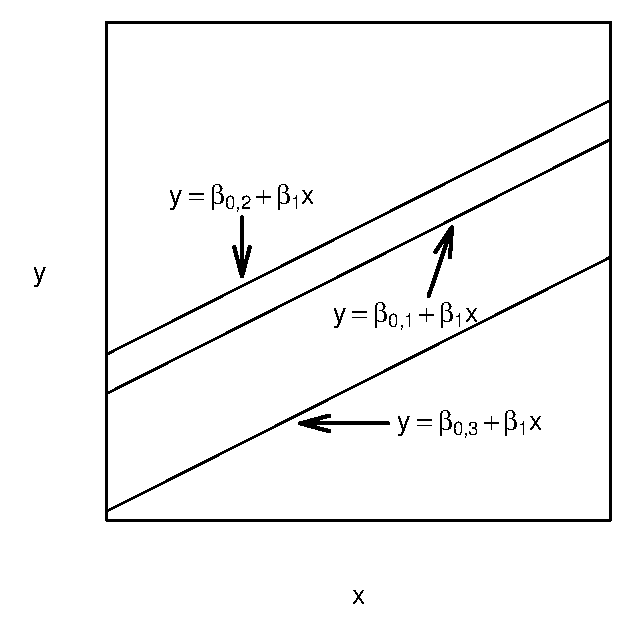
\includegraphics[width=0.45\textwidth]{Chapter4/F4TheoryVarIntConSlope.eps}
    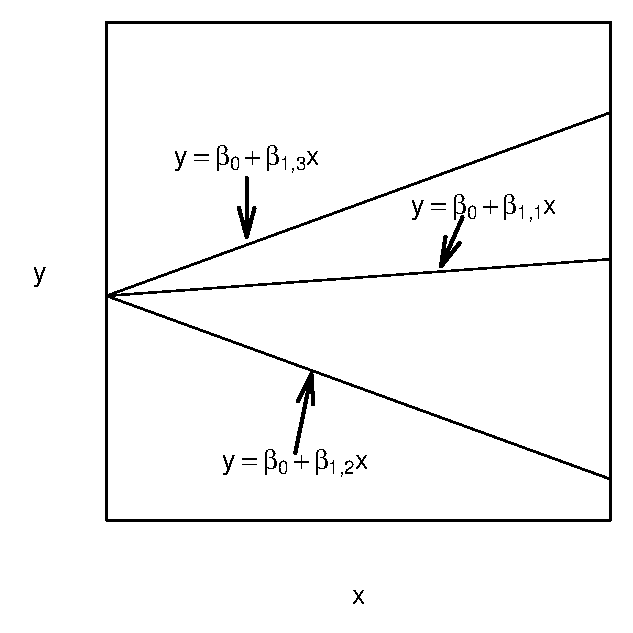
\includegraphics[width=0.45\textwidth]{Chapter4/F4TheoryConIntVarSlope.eps}
    \hfill  $~~~$
     \parbox[t]{2.5in}{\caption{\label{F4:TheoryVarIntConSlope} \small  Plot of the expected response versus the covariate for the regression model
with variable intercept and constant slope.}} \hfill
    \parbox[t]{2.5in}{\caption{\label{F4:TheoryConIntVarSlope} \small  Plot of the expected response versus the covariate for the regression model
with constant intercept and variable slope.}}
  \end{center}
\end{figure}


\begin{figure}[htp]
  \begin{center}
    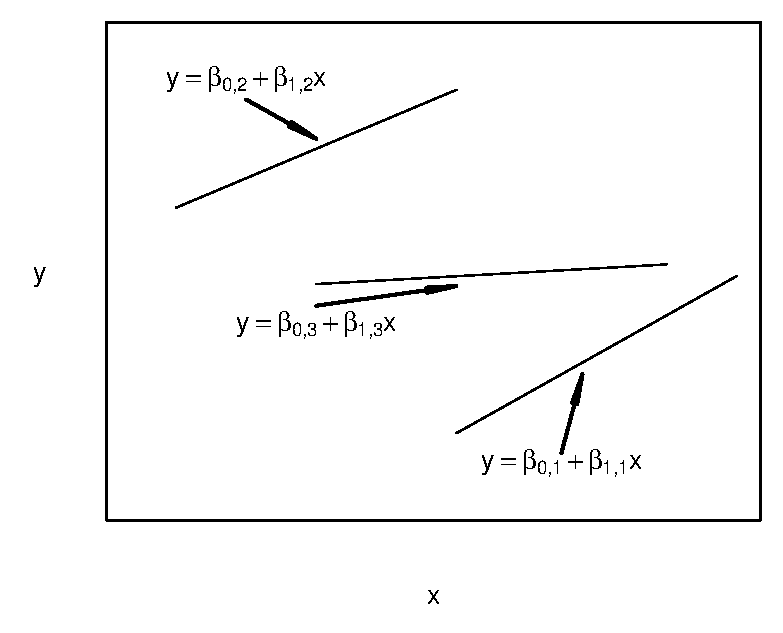
\includegraphics[width=.6\textwidth]{Chapter4/F4TheoryVarIntVarSlope.eps}
    \caption{\label{F4:TheoryVarIntVarSlope} \small  Plot of the expected response versus the covariate for the regression model
with variable intercept and variable slope.}
  \end{center}
\end{figure}

For each model presented in Table \ref{T4:OneFactorCovariate},
parameter estimates can be calculated using the method of least
squares. As usual, this means writing the expected response, E
$y_{ij}$, as a function of known variables and unknown parameters.
For the regression model with variable intercept and constant slope,
the least squares estimates can be expressed compactly as:

\begin{equation*}
b_1=\frac{\sum_{j=1}^{c}\sum_{i=1}^{n_j}(x_{ij}-\bar{x}_j)(y_{ij}-\bar{%
y}_j)}{\sum_{j=1}^{c}\sum_{i=1}^{n_j}(x_{ij}-\bar{x}_j)^2}
\end{equation*}
and $b_{0,j}=\bar{y}_j-b_1\bar{x}_j$. Similarly, the least
squares estimates for the regression model with variable intercept
and slope can be expressed as:

\begin{equation*}
b_{1,j}=\frac{\sum_{i=1}^{n_j}(x_{ij}-\bar{x}_j)(y_{ij}-\bar{y}_j)}{%
\sum_{i=1}^{n_j}(x_{ij}-\bar{x}_j)^2}
\end{equation*}
and $b_{0,j}=\bar{y}_j-b_1\bar{x}_j$. With these parameter
estimates, fitted values may be calculated.

For each model, fitted values are defined to be the expected response with
the unknown parameters replaced by their least squares estimates.
For example, for the regression model with variable intercept and
constant slope the fitted values are
$\hat{y}_{ij}=b_{0,j}+b_1x_{ij}$.

\linejed


\empexjed{WiscHospCosts} \index{datasets!Wisconsin hospital
costs}\index{actuarial \& financial terms and concepts!health
provider!fee for service, FFS} \index{actuarial \& financial terms
and concepts!health provider!health maintenance organization, HMO}

\textbf{Example: Wisconsin Hospital Costs.}\ecaptionjed{Hospital
Charges} We now study the impact of various predictors on hospital
charges in the state of Wisconsin. Identifying predictors of
hospital charges can provide direction for hospitals, government,
insurers and consumers in controlling these variables that in turn
leads to better control of hospital costs. The data for the year
1989 were obtained from the Office of Health Care Information,
Wisconsin's Department of Health and Human Services. Cross sectional
data are used, which details the 20 diagnosis related group (DRG)
discharge costs for hospitals in the state of Wisconsin, broken down
into nine major health service areas and three types of providers
(Fee for service, HMO, and other). Even though there are 540
potential DRG, area and payer combinations $(20\times 9\times
3=540)$, only 526 combinations were actually realized in the 1989
data set. Other predictor variables included the logarithm of the
total number of discharges (NO DSCHG) and total number of hospital
beds (NUM BEDS) for each combination. The response variable is the
logarithm of total hospital charges per number of discharges
(CHGNUM). To streamline the presentation, we now consider only costs
associated with three diagnostic related groups (DRGs), DRG \#209,
DRG \#391 and DRG \#430.

The covariate, $x$, is the natural logarithm of the number of
discharges. In ideal settings, hospitals with more patients enjoy
lower costs due to economies of scale. In non-ideal settings,
hospitals may not have excess capacity and thus, hospitals with more
patients have higher costs. One purpose of this analysis is to
investigate the relationship between hospital costs and hospital
utilization.

Recall that our measure of hospital charges is the logarithm of
costs per discharge $(y)$. The scatter plot in Figure
\ref{F4:CostperNumber} gives a preliminary idea of the relationship
between $y$ and $x$. We note that there appears to be a negative
relationship between $y$ and $x$.

The negative relationship between $y$ and $x$ suggested by Figure
\ref{F4:CostperNumber} is misleading and is induced by an
\textit{omitted variable}, the category of the cost (DRG). To see
the joint effect of the categorical variable DRG and the continuous
variable $x$, in Figure \ref{F4:DRGbyNumber} is a plot of $y$ versus
$x$ where the plotting symbols are codes for the level of the
categorical variable. From this plot, we see that the level of cost
varies by level of the factor DRG. Moreover, for each level of DRG,
the slope between $y$ and $x$ is either zero or positive. The slopes
are not negative, as suggested by Figure \ref{F4:CostperNumber}.

\begin{figure}[htp]
  \begin{center}
    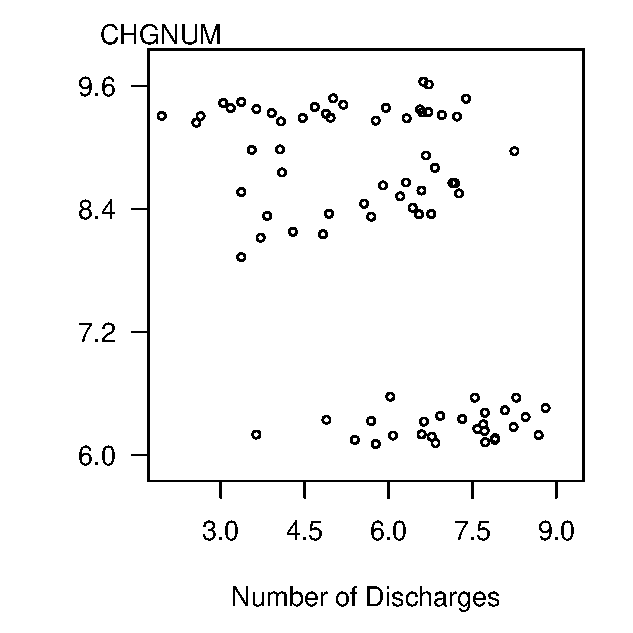
\includegraphics[width=0.45\textwidth]{Chapter4/F4CostperNumber.eps}
    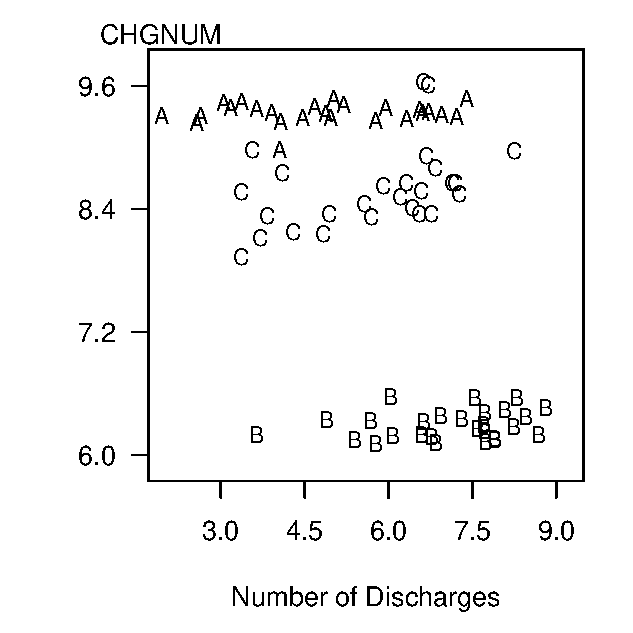
\includegraphics[width=0.45\textwidth]{Chapter4/F4DRGbyNumber.eps}
    \hfill  $~~~$
    \parbox[t]{2.5in}{\caption{\label{F4:CostperNumber} \small  Plot of natural logarithm of cost per discharge versus natural
logarithm of the number of discharges. This plot suggest a
misleading negative relationship.}} \hfill
    \parbox[t]{2.5in}{\caption{\label{F4:DRGbyNumber} \small  Letter plot of natural logarithm of cost per discharge versus natural
logarithm of the number of discharges by DRG. Here, A is for DRG
\#209, B is for DRG \#391 and C is for DRG \#430.}}
  \end{center}
\end{figure}


\begin{table}[h]
\caption{\label{T4:DRGModels} Wisconsin Hospital Cost Models
Goodness of Fit.}
\begin{tabular}{lccrcc}
\hline & Model & Error & Error  &  & Error  \\
& degrees & degrees
& Sum & $R^2$  & Mean \\
Model Description & of freedom & of freedom & of Squares & (\%) &
Square
\\ \hline
One factor ANOVA & 2 &
76 & \multicolumn{1}{r}{$9.396$} & \multicolumn{1}{r}{$%
93.3$} & \multicolumn{1}{r}{$0.124$} \\
Regression with constant intercept & 1 & 77 &
\multicolumn{1}{r}{$115.059$} &
\multicolumn{1}{r}{$18.2$} & \multicolumn{1}{r}{$1.222$} \\
~~~and slope & & & & &  \\
Regression with variable intercept &3 & 75 &
\multicolumn{1}{r}{$7.482$} &
\multicolumn{1}{r}{$94.7$} & \multicolumn{1}{r}{$0.100$} \\
~~~and constant slope &  & &  &  &  \\
Regression with constant intercept & 3 & 75 &
\multicolumn{1}{r}{$14.048$} &
\multicolumn{1}{r}{$90.0$} & \multicolumn{1}{r}{$0.187$} \\
~~~and variable slope &  &  &  &  & \\
Regression with variable intercept & 5 & 73 &
\multicolumn{1}{r}{$5.458$} &
\multicolumn{1}{r}{$96.1$} & \multicolumn{1}{r}{$0.075$} \\
~~~and slope &  & & &  &  \\
\hline \multicolumn{6}{l}{\textit{Note}: These models represent
combinations of one factor and one covariate.} \\
\end{tabular}

\end{table}

Each of the five models defined in Table \ref{T4:OneFactorCovariate}
was fit to this subset of the Hospital case study. The summary
statistics are in Table \ref{T4:DRGModels}. For this data set, there
are $n=79$ observations and $c=3$ levels of the DRG factor. For each
model, the model degrees of freedom is the number of model
parameters minus one. The error degrees of freedom is the number of
observations minus the number of model parameters.

Using binary variables, each of the models in Table
\ref{T4:OneFactorCovariate} can be written in a regression format.
As we have seen in Section \ref{S4:SeveralCoeff}, when a model can
be written as a subset of another, larger model, we have formal
testing procedures available to decide which model is more
appropriate. To illustrate this testing procedure with our DRG
example, from Table \ref{T4:DRGModels} and the associated plots, it
seems clear that the DRG factor is important. Further, a $t$-test,
not presented here, shows that the covariate $x$ is important. Thus,
let's compare the full model E $y_{ij} = \beta_{0,j} + \beta_{1,j}x$
to the reduced model E $y_{ij}=\beta_{0,j}+\beta_1x$. In other
words, is there a different slope for each DRG?

Using the notation from Section \ref{S4:SeveralCoeff}, we call the
variable intercept and slope the full model. Under the null
hypothesis, $H_0: \beta_{1,1}=\beta_{1,2}=\beta_{1,3}$, we get the
variable intercept, constant slope model. Thus, using the $F$-ratio
in equation (\ref{E4:FratioErrSumSquares}), we have

\begin{equation*}
F\text{-ratio}=\frac{(Error~SS)_{reduced}-(Error~SS)_{full}}{ps_{full}^2}=\frac{{7.482-5.458}}{2(0.075)}=13.535.
\end{equation*}
The 95$th$ percentile from the $F$-distribution with
$df_1=p=2$ and $df_2=(df)_{full}=73$ is approximately 3.13. Thus,
this test leads us to reject the null hypothesis and declare the
alternative, the regression model with variable intercept and
variable slope, to be valid.

\linejed


\subsubsection*{Combining Two Factors}

We have seen how to combine covariates as well as a covariate and
factor, both additively and with interactions. In the same fashion,
suppose that we have two factors, say gender (two levels,
male/female) and age (three levels, young/middle/old). Let the
corresponding binary variables be $x_1$ to indicate whether the
observation represents a female, $x_2$ to indicate whether the
observation represents a young person and $x_3$ to indicate whether
the observation represents a middle-aged person.

An \emph{additive model} for these two factors may use the
regression function

\begin{equation*}
\mathrm{E}~y = \beta_0 + \beta_1 x_1 + \beta_2 x_2+ \beta_3 x_3.
\end{equation*}
As we have seen, this model is simple to interpret. For example, we
can interpret $\beta_1$ to be the gender effect, holding age
constant.\index{regression model!two factor additive}

We can also incorporate two interaction terms, $x_1 x_2$ and $x_1
x_3$. Using all five explanatory variables yields the regression
function

\begin{equation}\label{E4:TwoFactorFunction}
\mathrm{E}~y = \beta_0 + \beta_1 x_1 + \beta_2 x_2+ \beta_3 x_3 +
\beta_4 x_1 x_2 + \beta_5 x_1 x_3 .
\end{equation}
Here, the variables $x_1,$ $x_2$ and $x_3$ are known as the\textit{
main effects}. Table \ref{T4:TwoFactorModel} helps interpret this
equation. Specifically, there are six types of people that we could
encounter, males and females who are young, middle-aged or old. We
have six parameters in equation (\ref{E4:TwoFactorFunction}). Table
\ref{T4:TwoFactorModel} provides the link between the parameters and
the types of people. By using the interaction terms, we do not
impose any prior specifications on the additive effects of each
factor. From Table \ref{T4:TwoFactorModel}, we see that the
interpretation of the regression coefficients in equation
(\ref{E4:TwoFactorFunction}) is not straightforward. However, using
the additive model with interaction terms is equivalent to creating
a new categorial variable with six levels, one for each type of
person. If the interaction terms are critical in your study, you may
wish to create a new factor that incorporates the interaction terms
simply for ease of interpretation.\index{regression model!two factor
interaction}

\begin{table}[htp]
\caption{\label{T4:TwoFactorModel} Regression Function for a Two
Factor Model with Interactions}
\begin{tabular}{lc|ccccc|c}
\hline Gender & Age & $x_1$ & $x_2$ &  $x_3$ &  $x_4$ &  $x_5$ &
Regression Function (\ref{E4:TwoFactorFunction})
\\
\hline
Male & Young    & 0 & 1 & 0 & 0 & 0 & $\beta_0 +\beta_2$\\
Male & Middle   & 0 & 0 & 1 & 0 & 0 & $\beta_0 +\beta_3$\\
Male & Old      & 0 & 0 & 0 & 0 & 0 & $\beta_0 $\\
Female & Young  & 1 & 1 & 0 & 1 & 0 & $\beta_0 +\beta_1+\beta_2+\beta_4$\\
Female & Middle & 1 & 0 & 1 & 0 & 1 & $\beta_0 +\beta_1+\beta_3+\beta_5$\\
Female & Old    & 1 & 0 & 0 & 0 & 0 & $\beta_0 +\beta_1$\\
 \hline
\end{tabular}
 \end{table}

Extensions to more than two factors follow in a similar fashion. For
example, suppose that you are examining the behavior of firms with
headquarters in ten geographic regions, two organizational
structures (profit versus non-profit) with four years of data. If
you decide to treat each variable as a factor and want to model all
interaction terms, then this is equivalent to a factor with $10
\times 2 \times 4 =80$ levels. Models with interaction terms can
have a substantial number of parameters and the analyst must be
prudent when specifying interactions to be considered.



\subsubsection*{General Linear Model}\index{regression model!general
linear model}

The general linear model extends the linear regression model in two
ways. First, explanatory variables may be continuous, categorical or
a combination. The only restriction is that they enter linearly such
that the resulting regression function
\begin{equation}\label{E4:GenLinearModel}
\mathrm{E}~y = \beta_0 + \beta_1 x_1 + \ldots \ + \beta_k x_k
\end{equation}
is a linear combination of coefficients. As we have seen, we can
square continuous variables or take other nonlinear transforms (such
as logarithms) as well as use binary variables to represent
categorical variables, so this ``restriction,'' as the name
suggests, allows for a broad class of general functions to represent
data.

The second extension is that the explanatory variables may be linear
combinations of one another in the general linear model. Because of
this, in the general linear model case, the parameter estimates need
not be unique. However, an important feature of the general linear
model is that the resulting fitted values turn out to be unique,
using the method of least squares.

For example, in Section 4.3 we saw that the one factor ANOVA model
could be expressed as a regression model with $c$ indicator
variables. However, if we had attempted to estimate the model in
equation (\ref{E4:OneFactorTau}), the method of least squares would
not have arrived at a unique set of regression coefficient
estimates. The reason is that, in equation (\ref{E4:OneFactorTau}),
each explanatory variable can be expressed as a linear combination
of the others. For example, observe that $x_c = 1 - (x_1 + x_2 +
\ldots + x_{c-1})$.

The fact that parameter estimates are not unique is a drawback, but
not an overwhelming one. The assumption that the explanatory
variables are not linear combinations of one another means that we
can compute unique estimates of the regression coefficients using
the method of least squares. In terms of matrices, because the
explanatory variables are not linear combinations of one another,
the matrix $\mathbf{X}^{\prime}\mathbf{X}$ is not invertible.

Specifically, suppose that we are considering the regression
function in equation (\ref{E4:GenLinearModel}) and, using the method
of least squares, our regression coefficient estimates are $b_0^{o},
b_1^{o}, \ldots, b_k^{o}$. This set of regression coefficients
estimates minimizes our error sum of squares, but there may be other
sets of coefficients that also minimize the error sum of squares.
The fitted values are computed as $\hat{y}_i = b_0^{o} + b_1^{o}
x_{i1} + \ldots + b_k^{o} x_{ik}$. It can be shown that the
resulting fitted values are unique, in the sense that any set of
coefficients that minimize the error sum of squares produce the same
fitted values (see Section \ref{S4:GeneralLinearModel}).

Thus, for a set of data and a specified general linear model, fitted
values are unique. Because residuals are computed as observed
responses minus fitted values, we have that the residuals are
unique. Because residuals are unique, we have the error sums of
squares are unique. Thus, it seems reasonable, and is true, that we
can use the general test of hypotheses described in Section
\ref{S4:SeveralCoeff} to decide whether collections of explanatory
variables are important.

To summarize, for general linear models, parameter estimates may not
be unique and thus not meaningful. An important part of regression
models is the interpretation of regression coefficients. This
interpretation is not necessarily available in the general linear
model context. However, for general linear models, we may still
discuss the important of an individual variable or collection of
variables through partial \textit{F}-tests. Further, fitted values,
and the corresponding exercise of prediction, works in the general
linear model context. The advantage of the general linear model
context is that we need not worry about the type of restrictions to
impose on the parameters. Although not the subject of this text,
this advantage is particularly important in complicated experimental
designs used in the life sciences. The reader will find that general
linear model estimation routines are widely available in statistical
software packages available on the market today.



\section{Further Reading and References}

There are several good linear model books that focus on categorical
variables and analysis of variance techniques. Hocking (2003) and
Searle (1987) are good examples.

\bigskip


\textbf{Chapter References}

\begin{multicols}{2}

\scalefont{0.9}

Hocking, Ronald R. (2003). \textit{Methods and Applications of
Linear Models: Regression and the Analysis of Variance}. Wiley, New
York.

Keeler, Emmett B., and  John E. Rolph (1988). The demand for
episodes of treatment in the Health Insurance Experiment.
\emph{Journal of Health Economics} 7: 337-367.

Searle, Shayle R. (1987). \textit{Linear Models for Unbalanced
Data}. John Wiley \& Sons, New York.


\scalefont{1.1111}

\end{multicols}

\bigskip


\section{Exercises}

\scalefont{0.90}

\begin{exercises}

\item In this exercise, we consider relating two statistics that summarize how well a regression model fits,
the $F$-ratio and $R^2$, the coefficient of determination. (Here,
the $F$-ratio is the statistic used to test model adequacy, not a
partial $F$ statistic.)

a.  Write down both $R^2$ in terms of $Error~SS$ and
$Regression~SS$.

b. Write down $F$-ratio in terms of $Error~SS$, $Regression~SS$ ,
$k$ and $n$.

c. Establish the algebraic relationship
\begin{equation*}
F-\textrm{ratio} = \frac{R^2}{1-R^2} \frac{n-(k+1)}{k}.
\end{equation*}

d.  Suppose that $n = 40$, $k = 5$ and $R^2 = 0.20$. Calculate the
$F$-ratio. Perform the usual test of model adequacy to determine
whether or not the five explanatory variables jointly significantly
affect the response variable.

e.  Suppose that $n = 400$ (not 40), $k = 5$ and $R^2 = 0.20$.
Calculate the $F$-ratio. Perform the usual test of model adequacy to
determine whether or not the five explanatory variables jointly
significantly affect the response variable.

\empexjed{HospitalCosts}\index{datasets!hospital costs}

\item \textbf{Hospital Costs.}\label{Ex:HospExpend4} This exercise considers
hospital expenditures data provided by the US Agency for Healthcare
Research and Quality (AHRQ) and described in Exercise
1.\ref{Ex:HospExpend}.

a. Produce a scatter plot, correlation and a linear regression of
LNTOTCHG on AGE. Is AGE a significant predictor of LNTOTCHG?

b. You are concerned that newborns follow a different pattern than
other ages. Create a binary variable that indicates whether or not
AGE equals zero. Run a regression using this binary variable and AGE
as explanatory variables. Is the binary variable statistically
significant?

c. Now examine the gender effect, using the binary variable FEMALE
that is one if the patient is female and zero otherwise. Run a
regression using AGE and FEMALE as explanatory variables. Run a
second regression running these two variables with an interaction
term. Comment on whether the gender effect is important in either
model.

d. Now consider the type of admission, APRDRG, an acronym for ``all
patient refined diagnostic related group.'' This is a categorical
explanatory variable that provides information on the type of
hospital admission. There are several hundred levels of this
category. For example, level 640 represents admission for a normal
newborn, with neonatal weight greater than or equal to 2.5
kilograms. As another example, level 225 represents admission
resulting in an appendectomy.

d(i). Run a one-factor ANOVA model, using APRDRG to predict
LNTOTCHG. Examine the $R^2$ from this model and compare it to the
coefficient of determination of the linear regression model of
LNTOTCHG on AGE. Based on this comparison, which model do you think
is preferred?

d(ii). For the one-factor model in part d(i), provide a 95\%
confidence interval for LNTOTCHG for level 225 corresponding to an
appendectomy. Convert your final answer from logarithmic dollars to
dollars via exponentiation.

d(iii). Run a regression model of APRDRG, FEMALE and AGE on
LNTOTCHG. State whether AGE is a statistically significant predictor
of LNTOTCHG. State whether FEMALE is a statistically significant
predictor of LNTOTCHG.

\empexjed{WiscNursingHome}\index{datasets!nursing home utilization}

\item \textbf{Nursing Home Utilization.}\label{Ex:NursHome4} This exercise considers nursing
home data provided by the Wisconsin Department of Health and Family
Services (DHFS) and described in Exercises 1.\ref{Ex:NursHome},
2.\ref{Ex:NursHome2a} and 2.\ref{Ex:NursHome2b}.

In addition to the size variables, we also have information on
several binary variables. The variable URBAN is used to indicate the
facility's location. It is one if the facility is located in an
urban environment and zero otherwise. The variable MCERT indicates
whether the facility is Medicare-certified. Most, but not all,
nursing homes are certified to provide Medicare-funded care. There
are three organizational structures for nursing homes. They are
government (state, counties, municipalities), for-profit businesses,
and tax-exempt organizations. Periodically, facilities may change
ownership and, less frequently, ownership type. We create two binary
variables PRO and TAXEXEMPT to denote for-profit business and
tax-exempt organizations, respectively. Some nursing homes opt not
to purchase private insurance coverage for their employees. Instead,
these facilities directly provide insurance and pension benefits to
their employees; this is referred to as ``self funding of
insurance." We use binary variable SELFFUNDINS to denote it.

You decide to examine the relationship between LOGTPY(y) and the
explanatory variables. Use cost report year 2001 data, and do the
following analysis.

a. There are three levels of organizational structures, but we only
use two binary variables (PRO and TAXEXEMPT). Explain why.

b. Run a one-way analysis of variance using TAXEXEMPT as the factor.
Decide whether or not tax-exempt is an important factor in
determining LOGTPY. State your null hypothesis, alternative
hypothesis and all components of the decision-making rule. Use a 5\%
level of significance.

c. Run a one-way analysis of variance using MCERT as the factor.
Decide whether or not location is an important factor in determining
LOGTPY.

c(i). Provide a point estimate of LOGTPY for a nursing facility that
is not Medicare-Certified.

c(ii).  Provide a 95\% confidence interval for your point estimate
in part c(i).

d. Run a regression model using the binary variables, URBAN, PRO,
TAXEXEMPT, SELFFUNDINS, and MCERT. Find $R^2$. Which variables are
statistically significant?

e. Run a regression model using all explanatory variables,
LOGNUMBED, LOGSQRFOOT, URBAN, PRO, TAXEXEMPT, SELFFUNDINS, and
MCERT. Find $R^2$. Which variables are statistically significant?

e(i). Calculate the partial correlation between LOGTPY and
LOGSQRFOOT. Compare this to the correlation between LOGTPY and
LOGSQRFOOT. Explain why the partial correlation is small.

e(ii). Compare the low level of the $t$-ratios (for testing the
importance of individual regression coefficients) and the high level
of the $F$-ratio (for testing model adequacy). Describing the
seeming inconsistency, and provide an explanation for this
inconsistency.

\empexjed{AutoClaims}\index{datasets!automobile insurance claims}

\item \textbf{Automobile Insurance Claims.}\label{Ex:AutoClaims4} Refer to Exercise
1.\ref{Ex:AutoClaims}.

a. Run a regression of LNPAID on AGE. Is AGE a statistically
significant variable? To respond to this question, use a formal test
of hypothesis. State your null and alternative hypotheses,
decision-making criterion, and your decision-making rule. Also
comment on the goodness of fit of this variable.

b. Consider using class as a single explanatory variable. Use the
one factor to estimate the model and respond to the following
questions.

b(i). What is the point estimate of claims in class C7, drivers
50-69, driving to work or school, less than 30 miles per week with
annual mileage under 7500, in natural logarithmic units?

b(ii). Determine the corresponding 95\% confidence interval of
expected claims, in natural logarithmic units.

b(iii). Convert the 95\% confidence interval of expected claims that
you determined in part b(ii) to dollars.

c. Run a regression of LNPAID on AGE, GENDER and the categorical
variables STATE CODE and CLASS.

c(i). Is GENDER a statistically significant variable? To respond to
this question, use a formal test of hypothesis. State your null and
alternative hypotheses, decision-making criterion, and your
decision-making rule.

c(ii). Is CLASS a statistically significant variable? To respond to
this question, use a formal test of hypothesis. State your null and
alternative hypotheses, decision-making criterion, and your
decision-making rule.

c(iii). Use the model to provide a point estimate of claims in
dollars (not log dollars) for a male age 60 in state 2 in class C7.

c(iv). Write down the coefficient associated with class C7 and
interpret this coefficient.

\empexjed{WiscLottery}\index{datasets!Wisconsin lottery sales}

\item \textbf{Wisconsin Lottery Sales.}\label{Ex:Lottery4}
This exercise considers State of Wisconsin lottery sales data that
were described in Section 2.1 and examined in Exercise
3.\ref{Ex:Lottery3}.

\textbf{Part 1:} You decide to examine the relationship between
SALES ($y$) and all eight explanatory variables (PERPERHH, MEDSCHYR,
MEDHVL, PRCRENT, PRC55P, HHMEDAGE, MEDINC, and POP).

a. Fit a regression model of SALES on all eight explanatory
variables.

b. Find $R^2$.

b(i). Use it to calculate the correlation coefficient between the
observed and fitted values.

b(ii). You want to use $R^2$ to test the adequacy of the model in
part (a). Use a formal test of hypothesis. State your null and
alternative hypothesis, decision-making criterion, and your
decision-making rules.

c. Test whether POP, MEDSCHYR and MEDHVL are jointly important
explanatory variables for understanding SALES.


\textbf{Part 2:} After the preliminary analysis in Part 1, you
decide to examine the relationship between SALES($y$) and POP,
MEDSCHYR, and MEDHVL.

a. Fit a regression model of SALES on these three explanatory
variables.

b. Has the coefficient of determination decreased from the eight
variable regression model to the three variable model? Does this
mean that the model is not improved or does it provide little
information? Explain your response.

c. To state formally whether one should use the three or eight
variable model, use a partial $F$-test. State your null and
alternative hypotheses, decision-making criterion, and your
decision-making rules.

\empexjed{NAICExpense}\index{datasets!insurance company expenses}

\item \textbf{Insurance Company Expenses.}\label{Ex:NAICExpense4}
This exercise considers insurance company data from the NAIC and
described in Exercises 1.\ref{Ex:NAICExpense} and
3.\ref{Ex:NAICExpense3}.


a. Are the quadratic terms important?

Consider a linear model of LNEXPENSES on twelve explanatory
variables. For the explanatory variables, include assets, GROUP,
both versions of losses and gross premiums, as well as the two BLS
variables. Also include the square each of the two loss and the two
gross premium variables.

Test whether the four squared terms are jointly statistically
significant, using a partial $F$-test. State your null and
alternative hypotheses, decision-making criterion, and your
decision-making rules.

b. Are the interaction terms with GROUP important?

Omit the two BLS variables, so that now there are eleven variables,
assets, GROUP, both versions of losses and gross premiums, as well
as interactions of GROUP with assets and both versions of losses and
gross premiums.

Test whether the five interaction terms are jointly statistically
significant, using a partial $F$-test. State your null and
alternative hypotheses, decision-making criterion, and your
decision-making rules.

c. You are examining a company that is not in the sample with values
LOSSLONG = 0.025, LOSSSHORT = 0.040, GPWPERSONAL= 0.050, GPWCOMM=
0.120, ASSETS = 0.400,CASH= 0.350, and GROUP = 1.

Use the eleven variable interaction model in part (b) to produce a
95\% prediction interval for this company.

\empexjed{UNLifeExpectancy}

\item \textbf{National Life Expectancies.}\label{Ex:UNLIFE4} We
continue the analysis begun in Exercises 1.\ref{Ex:UNLIFE},
2.\ref{Ex:UNLIFE2} and 3.\ref{Ex:UNLIFE3}.

a. Consider the regression using three explanatory variables,
FERTILITY, PUBLICEDUCATION and lnHEALTH that you did in Exercise
3.\ref{Ex:UNLIFE3}. Test whether PUBLICEDUCATION and lnHEALTH are
jointly statistically significant, using a partial $F$-test. State
your null and alternative hypotheses, decision-making criterion, and
your decision-making rules. (Hint: Use the coefficient of
determination form for calculating the test statistic.) Provide an
approximate $p$-value for the test.

b. We now introduce the REGION variable, summarized in Table
\ref{Ex:UNLIFERegionStats}. A boxplot of life expectancies versus
REGION is given in Figure \ref{Ex:UNLIFEPlot3}. Describe what we
learn from the Table and boxplot about the effect of REGION on
LIFEEXP.


\begin{figure}[htp]
  \begin{center}
   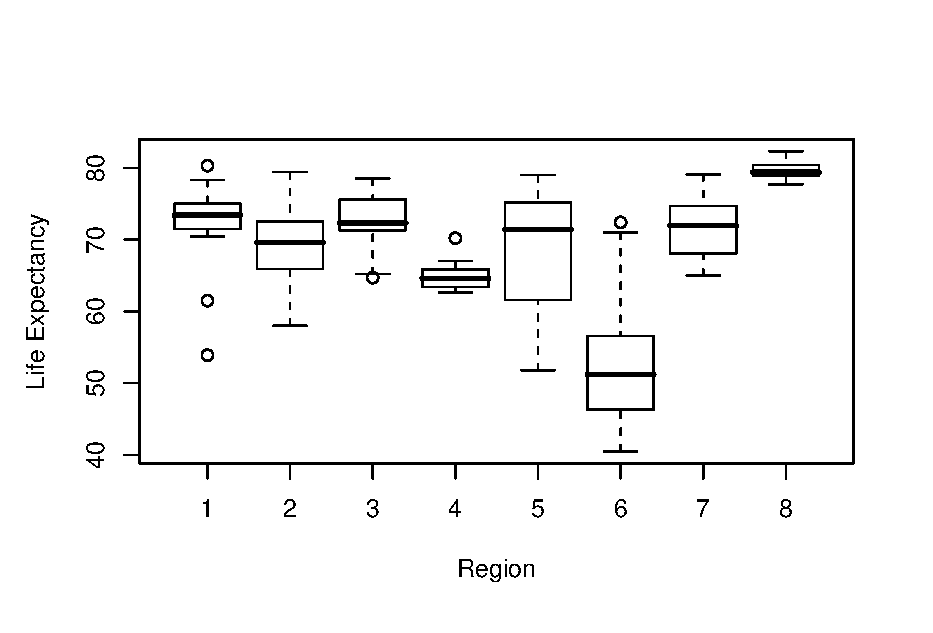
\includegraphics[width=0.6\textwidth]{Chapter4/UNLife3.eps}
   \caption{\label{Ex:UNLIFEPlot3} \small  Boxplots of LIFEEXP by REGION.}
  \end{center}
\end{figure}


\begin{table}[h]

\scalefont{0.8} \caption{\label{Ex:UNLIFERegionStats} \small Average
Life Expectancy by Region}
\begin{center}
\begin{tabular}{c|lcr}
\hline
    REGION & Region Description &     Number &       Mean \\ \hline
         1 & Arab States &         13 &       71.9 \\
         2 & East Asia and the Pacific &         17 &       69.1 \\
         3 & Latin American and the Carribean &         25 &       72.8 \\
         4 & South Asia &          7 &       65.1 \\
         5 & Southern Europe &          3 &       67.4 \\
         6 & Sub-Saharan Africa &         38 &       52.2 \\
         7 & Central and Eastern Europe &         24 &       71.6 \\
         8 & High Income OECD &         23 &       79.6 \\\hline
           & All          &        150 &     67.4       \\\hline
\end{tabular}
\end{center}\scalefont{1.25}
\end{table}

c. Fit a regression model using only the factor, REGION. Is REGION a
statistically significant determinant of LIFEEXP? State your null
and alternative hypotheses, decision-making criterion, and your
decision-making rules.

d. Fit a regression model using three explanatory variables,
FERTILITY, PUBLICEDUCATION and lnHEALTH, as well as the categorical
variable REGION.

d(i). You are examining a country is not in the sample with values
FERTILITY= 2.0, PUBLICEDUCATION= 5.0,  and lnHEALTH= 1.0. Produce
two predicted life expectancy values by assuming that the country is
from (1) an Arab state and (2) Sub-Sahara Africa.

d(ii). Provide a 95\% confidence interval for the difference in life
expectancies between an Arab state and a country from Sub-Sahara
Africa.

d(iii). Provide the (usual ordinary least squares) point estimate
for the difference in life expectancies between a country from
Sub-Sahara Africa and a high income OECD (Organization for Economic
Co-operation and Development) country.

\end{exercises}
\scalefont{1.1111}

\section{Technical Supplement - Matrix Expressions}
 \setcounter{equation}{12}
 \scalefont{0.9}
\subsection{Expressing Models with Categorical Variables in
Matrix Form}\label{S4:CatVarMatrix}

Chapter 3 showed how to write the regression model equation in the
form $\mathbf{y=X} \boldsymbol \beta + \boldsymbol \varepsilon$
where $\mathbf{X}$ is a matrix of explanatory variables. This form
permits straightforward calculation of regression coefficients,
$\mathbf{b} = \left(\mathbf{X}^{\prime}
\mathbf{X}\right)^{-1}\mathbf{X}^{\prime} \mathbf{y}$. This section
shows how the model and calculations reduce to simpler expressions
when the explanatory variables are categorical.


\textbf{One Categorical Variable Model.} Consider the model with one
categorical variable introduced in Section \ref{S4:OneFactor} with
$c$ levels of the categorical variable. From equation
(\ref{E4:OneFactor}), this model can be written as
\begin{equation}\label{E4:MatrixOneFactor}
\mathbf{y}=
\begin{bmatrix}
y_{1,1} \\
\cdot  \\
\cdot  \\
\cdot  \\
y_{n_1,1} \\
\cdot  \\
\cdot  \\
\cdot  \\
y_{1,c} \\
\cdot  \\
\cdot  \\
\cdot  \\
y_{n_{c},c}%
\end{bmatrix}
=
\begin{bmatrix}
1 & 0 & \cdot \cdot \cdot  & 0 \\
\cdot  & \cdot  & \cdot \cdot \cdot  & \cdot  \\
\cdot  & \cdot  & \cdot \cdot \cdot  & \cdot  \\
\cdot  & \cdot  & \cdot \cdot \cdot  & \cdot  \\
1 & 0 & \cdot \cdot \cdot  & \cdot  \\
\cdot  & \cdot  & \cdot \cdot \cdot  & \cdot  \\
\cdot  & \cdot  & \cdot \cdot \cdot  & \cdot  \\
\cdot  & \cdot  & \cdot \cdot \cdot  & \cdot  \\
0 & 0 & \cdot \cdot \cdot  & 1 \\
\cdot  & \cdot  & \cdot \cdot \cdot  & \cdot  \\
\cdot  & \cdot  & \cdot \cdot \cdot  & \cdot  \\
\cdot  & \cdot  & \cdot \cdot \cdot  & \cdot  \\
0 & 0 & \cdot \cdot \cdot  & 1%
\end{bmatrix}%
\begin{bmatrix}
\mu_1 \\
\cdot  \\
\cdot  \\
\cdot  \\
\mu_c
\end{bmatrix}
+
\begin{bmatrix}
\varepsilon_{1,1} \\
\cdot  \\
\cdot  \\
\cdot  \\
\varepsilon_{n_1,1} \\
\cdot  \\
\cdot  \\
\cdot  \\
\varepsilon_{1,c} \\
\cdot  \\
\cdot  \\
\cdot  \\
\varepsilon_{n_{c},c}
\end{bmatrix}
=\mathbf{X} \boldsymbol \beta + \boldsymbol \varepsilon .
\end{equation}
To make the notation more compact, we write $\mathbf{0}$ and
$\mathbf{1}$ for a column of zeros and ones, respectively. With this
convention, another way to express equation
(\ref{E4:MatrixOneFactor}) is

\begin{center}
\begin{equation}\label{E4:Matrix2OneFactor}
\mathbf{y}=%
\begin{bmatrix}
\mathbf{1}_1 & \mathbf{0}_1 & \cdot \cdot \cdot  & \mathbf{0}%
_1 \\
\mathbf{0}_2 & \mathbf{1}_2 & \cdot \cdot \cdot  & \mathbf{0}%
_2 \\
\cdot  & \cdot  & \cdot \cdot \cdot  & \cdot  \\
\cdot  & \cdot  & \cdot \cdot \cdot  & \cdot  \\
\cdot  & \cdot  & \cdot \cdot \cdot  & \cdot  \\
\mathbf{0}_c & \mathbf{0}_c & \cdot \cdot \cdot  & \mathbf{1}_c
\end{bmatrix}
\begin{bmatrix}
\mu_1 \\
\mu_2 \\
\cdot  \\
\cdot  \\
\cdot  \\
\mu_c%
\end{bmatrix}
+\boldsymbol \varepsilon = \mathbf{X} \boldsymbol \beta +
\boldsymbol \varepsilon .
\end{equation}
\end{center}

\noindent Here, $\mathbf{0}_1$ and $\mathbf{1}_1$ stand for vector
columns of length $n_1$ of zeros and ones, respectively, and
similarly for $\mathbf{0}_2, \mathbf{1}_2, \ldots, \mathbf{0}_c,
\mathbf{1}_c$.

Equation (\ref{E4:Matrix2OneFactor}) allows us to apply the
machinery developed for the regression model to the model with one
categorical variable. As an intermediate calculation, we have

\begin{center}
\begin{eqnarray}\label{E4:OneFactorXPrimeX}
(\mathbf{X^{\prime}X})^{-1} &=&\left(
\begin{bmatrix}
\mathbf{1}_1 & \mathbf{0}_2 & \cdot \cdot \cdot  & \mathbf{0}_c \\
\mathbf{0}_1 & \mathbf{1}_2 & \cdot \cdot \cdot  & \mathbf{0}_c \\
\cdot  & \cdot  & \cdot \cdot \cdot  & \cdot  \\
\cdot  & \cdot  & \cdot \cdot \cdot  & \cdot  \\
\cdot  & \cdot  & \cdot \cdot \cdot  & \cdot  \\
\mathbf{0}_1 & \mathbf{0}_2 & \cdot \cdot \cdot  & \mathbf{1}_c%
\end{bmatrix}^{\prime}%
\begin{bmatrix}
\mathbf{1}_1 & \mathbf{0}_1 & \cdot \cdot \cdot  & \mathbf{0}%
_1 \\
\mathbf{0}_2 & \mathbf{1}_2 & \cdot \cdot \cdot  & \mathbf{0}%
_2 \\
\cdot  & \cdot  & \cdot \cdot \cdot  & \cdot  \\
\cdot  & \cdot  & \cdot \cdot \cdot  & \cdot  \\
\cdot  & \cdot  & \cdot \cdot \cdot  & \cdot  \\
\mathbf{0}_{c} & \mathbf{0}_{c} & \cdot \cdot \cdot  & \mathbf{1}_c
\end{bmatrix} \notag
\right) ^{-1} \\
&=&%
\begin{bmatrix}
n_1 & 0 & \cdot \cdot \cdot  & 0 \\
0 & n_2 & \cdot \cdot \cdot  & 0 \\
\cdot  & \cdot  & \cdot \cdot \cdot  & \cdot  \\
\cdot  & \cdot  & \cdot \cdot \cdot  & \cdot  \\
\cdot  & \cdot  & \cdot \cdot \cdot  & \cdot  \\
0 & 0 & \cdot \cdot \cdot  & n_c%
\end{bmatrix}%
^{-1}=%
\begin{bmatrix}
\frac{1}{n_1} & 0 & \cdot \cdot \cdot  & 0 \\
0 & \frac{1}{n_2} & \cdot \cdot \cdot  & 0 \\
\cdot  & \cdot  & \cdot \cdot \cdot  & \cdot  \\
\cdot  & \cdot  & \cdot \cdot \cdot  & \cdot  \\
\cdot  & \cdot  & \cdot \cdot \cdot  & \cdot  \\
0 & 0 & \cdot \cdot \cdot  & \frac{1}{n_c}
\end{bmatrix}%
.
\end{eqnarray}
\end{center}

Thus, the parameter estimates are

\begin{center}
\begin{eqnarray}\label{E4:OneFactorXPrimeXinvXPrimey}
\mathbf{b} &=&%
\begin{bmatrix}
\hat{\mu}_1 \\
\cdot  \\
\cdot  \\
\cdot  \\
\hat{\mu}_{c}%
\end{bmatrix}%
=\mathbf{(X}^{\prime}\mathbf{X)}^{-1}\mathbf{X}^{\prime}\mathbf{y}=%
\begin{bmatrix}
\frac{1}{n_1} & 0 & \cdot \cdot \cdot  & 0 \\
0 & \frac{1}{n_2} & \cdot \cdot \cdot  & 0 \\
\cdot  & \cdot  & \cdot \cdot \cdot  & \cdot  \\
\cdot  & \cdot  & \cdot \cdot \cdot  & \cdot  \\
\cdot  & \cdot  & \cdot \cdot \cdot  & \cdot  \\
0 & 0 & \cdot \cdot \cdot  & \frac{1}{n_c}
\end{bmatrix}
\begin{bmatrix}
\mathbf{1}_1 & \mathbf{0}_2 & \cdot \cdot \cdot  & \mathbf{0}_c \\
\mathbf{0}_1 & \mathbf{1}_2 & \cdot \cdot \cdot  & \mathbf{0}_c \\
\cdot  & \cdot  & \cdot \cdot \cdot  & \cdot  \\
\cdot  & \cdot  & \cdot \cdot \cdot  & \cdot  \\
\cdot  & \cdot  & \cdot \cdot \cdot  & \cdot  \\
\mathbf{0}_1 & \mathbf{0}_2 & \cdot \cdot \cdot  & \mathbf{1}_c%
\end{bmatrix} ^{\prime}
\begin{bmatrix}
y_{1,1} \\
\cdot  \\
\cdot  \\
\cdot  \\
y_{n_1,1} \\
\cdot  \\
\cdot  \\
\cdot  \\
y_{1,c} \\
\cdot  \\
\cdot  \\
\cdot  \\
y_{n_{c},c}%
\end{bmatrix} \notag
\\
&=&%
\begin{bmatrix}
\frac{1}{n_1} & 0 & \cdot \cdot \cdot  & 0 \\
0 & \frac{1}{n_2} & \cdot \cdot \cdot  & 0 \\
\cdot  & \cdot  & \cdot \cdot \cdot  & \cdot  \\
\cdot  & \cdot  & \cdot \cdot \cdot  & \cdot  \\
\cdot  & \cdot  & \cdot \cdot \cdot  & \cdot  \\
0 & 0 & \cdot \cdot \cdot  & \frac{1}{n_c}
\end{bmatrix}
\begin{bmatrix}
\sum_{i=1}^{n_1}y_{i1} \\
\cdot  \\
\cdot  \\
\cdot  \\
\sum_{i=1}^{n_{c}}y_{ic}%
\end{bmatrix}%
=%
\begin{bmatrix}
\bar{y}_1 \\
\cdot  \\
\cdot  \\
\cdot  \\
\bar{y}_c
\end{bmatrix} .
\end{eqnarray}
\end{center}

We have seen that the least squares estimate of $\mu_j$,
$\bar{y}_j$, can been obtained directly from equation
(\ref{E4:OneFactor}). By rewriting the model in matrix regression
notation, we can appeal to linear regression model results and need
not prove properties of models with categorical variables from first
principles. That is, because this model is in regression format, we
immediately have all the properties of the regression model.

Telling your software package that a variable is categorical can
mean more efficient calculations, as in the calculations of the
least squares regression estimates in equation
(\ref{E4:OneFactorXPrimeXinvXPrimey}). Further, calculation of other
quantities can also be done more directly. As another example, we
have that the standard error of $\hat{\mu}_j$ is

\begin{equation*}
se(\hat{\mu}_j) = s ~ \sqrt{j\text{th \textit{diagonal element} of }
\mathbf{(X}^{\prime}\mathbf{X)}^{-1}} = s/\sqrt{n_j}.
\end{equation*}

\textbf{One Categorical and One Continuous Variable Model.} As
another illustration, we consider the variable intercept and
constant slope model in Table \ref{T4:OneFactorCovariate}. This can
be expressed as $\mathbf{y}= \mathbf{X \boldsymbol \beta +
\boldsymbol \varepsilon}$ where

\begin{equation}\label{E4:CategoricalContinuous}
\mathbf{X}=%
\begin{bmatrix}
\mathbf{1}_1 & \mathbf{0}_1 & \cdot \cdot \cdot  & \mathbf{0}%
_1 & \mathbf{x}_1 \\
\mathbf{0}_2 & \mathbf{1}_2 & \cdot \cdot \cdot  & \mathbf{0}%
_2 & \mathbf{x}_2 \\
\cdot  & \cdot  & \cdot \cdot \cdot  & \cdot  & \cdot  \\
\cdot  & \cdot  & \cdot \cdot \cdot  & \cdot  & \cdot  \\
\cdot  & \cdot  & \cdot \cdot \cdot  & \cdot  & \cdot  \\
\mathbf{0}_{c} & \mathbf{0}_{c} & \cdot \cdot \cdot  & \mathbf{1}_c & \mathbf{x}_{c}%
\end{bmatrix}%
\text{ \ \ \ \ and \ \ \ }\boldsymbol \beta=
\begin{bmatrix}
\beta_{01} \\
\beta_{02} \\
\cdot  \\
\cdot  \\
\cdot  \\
\beta_{0c} \\
\beta_1%
\end{bmatrix}
\end{equation}

\noindent As before, $\mathbf{0}_j$ and $\mathbf{1}_j$ stand for
vector columns of length $n_j$ of zeros and ones, respectively.
Further, $\mathbf{x}_j=(x_{1j},x_{2j},\ldots,x_{n_j,j})^{\prime}$ is
the column of the continuous variable at the $j$th level. Now,
straight-forward matrix algebra techniques provide the least squares
estimates.

\subsection{Calculating Least Squares Recursively}\label{S4:MatrixSuccess}

When computing regression coefficients using least squares,
$\mathbf{b} = \left( \mathbf{X}^{\prime}\mathbf{X}\right)^{-1}
\mathbf{X}^{\prime}\mathbf{y}$, for some applications, the dimension
of $\mathbf{X}^{\prime}\mathbf{X}$ can be large, causing
computational difficulties. Fortunately, for some problems, the
computations can be partitioned into smaller problems that can be
solved recursively.\index{least squares!recursive calculation}

\boxedjed \emph{Recursive Least Squares Calculation.} Suppose that
the regression function can be written as
\begin{equation}\label{E4:PartitionedModel}
\mathrm{E}~\mathbf{y} = \mathbf{X} \boldsymbol \beta = \left(
\mathbf{X}_1 : \mathbf{X}_2 \right) \left(
\begin{array}{c}
\boldsymbol \beta_1  \\
\boldsymbol \beta_2  \\
\end{array}
\right) ,
\end{equation}
where $\mathbf{X}_1$ has dimensions $n \times k_1$, $\mathbf{X}_2$
has dimensions $n \times k_2$, $k_1+k_2=k$, $\boldsymbol \beta_1 $
has dimensions $k_1 \times 1$ and $\boldsymbol \beta_2 $ has
dimensions $k_2 \times 1$. Define $\mathbf{Q}_1 = \mathbf{I} - \mathbf{X}_1
\left(\mathbf{X}_1^{\prime}\mathbf{X}_1 \right)^{-1}
\mathbf{X}_1^{\prime}.$ Then, the least squares estimator can be computed as:

\begin{equation}\label{E4:PartitionOLS}
\mathbf{b} = \left(
  \begin{array}{c}
    \mathbf{b}_1\\
    \mathbf{b}_2\\
  \end{array}
\right)
=
\left(
  \begin{array}{c}
    (\mathbf{X}_1^{\prime}\mathbf{X}_1)^{-1}\mathbf{X}_1^{\prime}
\left(
\mathbf{y} - \mathbf{X}_2 \mathbf{b}_2
\right)\\
   \left(\mathbf{X}_2^{\prime} \mathbf{Q}_1 \mathbf{X}_2
\right)^{-1} \mathbf{X}_2^{\prime} \mathbf{Q}_1\mathbf{y}\\
  \end{array}
\right) .
\end{equation}

\end{boxedminipage}
\bigskip

Equation(\ref{E4:PartitionOLS}) provides the first step in the
recursion. It can easily be iterated to allow for a more detailed
decomposition of $\mathbf{X}.$

\linejed

\textbf{Special Case: One Categorical and One Continuous Variable Model}.
To illustrate the relevance of equation (\ref{E4:PartitionOLS}), let us return to
the model summarized in equation (\ref{E4:CategoricalContinuous}). Here,
we saw that the dimension of $\mathbf{X}$ is $n \times (c+1)$ and so the dimension of
$\mathbf{X}^{\prime}\mathbf{X}$ is $(c+1) \times (c+1)$. Taking the inverse of this
matrix could be difficult if $c$ is large, say in the thousands. To apply equation
(\ref{E4:PartitionOLS}), we define
\begin{equation*}
\mathbf{X}_1=
\begin{bmatrix}
\mathbf{1}_1 & \mathbf{0}_1 & \cdot \cdot \cdot  & \mathbf{0}
_1 \\
\mathbf{0}_2 & \mathbf{1}_2 & \cdot \cdot \cdot  & \mathbf{0}
_2 \\
\cdot  & \cdot  & \cdot \cdot \cdot  & \cdot  \\
\cdot  & \cdot  & \cdot \cdot \cdot  & \cdot  \\
\cdot  & \cdot  & \cdot \cdot \cdot  & \cdot  \\
\mathbf{0}_{c} & \mathbf{0}_{c} & \cdot \cdot \cdot  & \mathbf{1}_c
\end{bmatrix}
\text{ \ \ \ \ and \ \ \ }\mathbf{X}_2 =
\begin{bmatrix}
\mathbf{x}_1\\
\mathbf{x}_2 \\
\cdot  \\
\cdot  \\
\cdot  \\
\mathbf{x}_c \\
\end{bmatrix} .
\end{equation*}
In this case, we have seen in equation (\ref{E4:OneFactorXPrimeX}) how it
is straightforward to compute
$\left(\mathbf{X}_1^{\prime}\mathbf{X}_1 \right)^{-1}$ without requiring
matrix inversion. This means that calculating $\mathbf{Q}_1$ is also straightforward. With this,
we can compute $\mathbf{X}_2^{\prime} \mathbf{Q}_1 \mathbf{X}_2$ and, because it is a scalar,
immediately get its inverse. This gives us $\mathbf{b}_2$ and then we use this result to
calculate $\mathbf{b}_1$. Although this procedure is not as direct as the our usual expression
$\mathbf{b} = \left( \mathbf{X}^{\prime}\mathbf{X}\right)^{-1}
\mathbf{X}^{\prime}\mathbf{y}$, it can be much more computationally efficient.

\linejed

To establish equation (\ref{E4:PartitionOLS}),
we use two results that are standard matrix algebra results on
inverses of partitioned matrices.

\textbf{Partitioned Matrix Results.} Suppose that we can partition
the $(p+q)\times (p+q)$ matrix $\mathbf{B}$ as
\begin{equation*}
\mathbf{B}=%
\begin{bmatrix}
\mathbf{B}_{11} & \mathbf{B}_{12} \\
\mathbf{B}_{12}^{\prime } & \mathbf{B}_{22}%
\end{bmatrix},
\end{equation*}
where $\mathbf{B}_{11}$ is a $p\times p$ invertible matrix,
$\mathbf{B}_{22}$ is a $q\times q$ invertible matrix, and
$\mathbf{B}_{12}$ is a $p\times q$ matrix. Then
\begin{equation}\label{E4:PartitionMatrixInverse1}
\mathbf{B}^{-1}=%
\begin{bmatrix}
\mathbf{C}_{11}^{-1} &
- \mathbf{B}_{11}^{-1}\mathbf{B}_{12}\mathbf{C}_{22}^{-1} \\
- \mathbf{C}_{22}^{-1} \mathbf{B}_{12}^{\prime} \mathbf{B}_{11}^{-1}
& \mathbf{C}_{22}^{-1}
\end{bmatrix},
\end{equation}
where
$\mathbf{C}_{11}=\mathbf{B}_{11}-\mathbf{B}_{12}\mathbf{B}_{22}^{-1}
\mathbf{B}_{12}^{\prime }$ and
$\mathbf{C}_{22}=\mathbf{B}_{22}\mathbf{-B}_{12}^{\prime
}\mathbf{B}_{11}^{-1}\mathbf{B}_{12}$. To check equation
(\ref{E4:PartitionMatrixInverse1}), simply multiply
$\mathbf{B}^{-1}$ by $\mathbf{B}$ to get $\mathbf{I}$, the identity
matrix. Further,
\begin{equation}\label{E4:PartitionMatrixInverse2}
\mathbf{C}_{11}^{-1}  = \mathbf{B}_{11}^{-1} + \mathbf{B}_{11}^{-1}
\mathbf{B}_{12} \mathbf{C}_{22}^{-1} \mathbf{B}_{12}^{\prime}
\mathbf{B}_{11}^{-1}.
\end{equation}

Now, we first write the least squares estimator as
\begin{eqnarray*}
\mathbf{b} &=& \left( \mathbf{X}^{\prime}\mathbf{X}\right)^{-1}
\mathbf{X}^{\prime} \mathbf{y} = \left( \left(
  \begin{array}{c}
    \mathbf{X}_1^{\prime} \\
    \mathbf{X}_2^{\prime} \\
  \end{array}
\right)
 \left( \mathbf{X}_1 : \mathbf{X}_2 \right)\right)^{-1}
\left(
  \begin{array}{c}
    \mathbf{X}_1^{\prime} \\
    \mathbf{X}_2^{\prime} \\
  \end{array}
\right) \mathbf{y} \\
&=& \left(
  \begin{array}{cc}
    \mathbf{X}_1^{\prime} \mathbf{X}_1 &\mathbf{X}_1^{\prime} \mathbf{X}_2  \\
   \mathbf{X}_2^{\prime} \mathbf{X}_1  & \mathbf{X}_2^{\prime} \mathbf{X}_2  \\
  \end{array}
 \right)^{-1}
\left(
  \begin{array}{c}
    \mathbf{X}_1^{\prime}  \mathbf{y}\\
    \mathbf{X}_2^{\prime}  \mathbf{y}\\
  \end{array}
\right) = \left(
  \begin{array}{c}
    \mathbf{b}_1\\
    \mathbf{b}_2\\
  \end{array}
\right) .
\end{eqnarray*}
To apply the partitioned matrix results, we define
\begin{equation*}
\mathbf{Q}_j = \mathbf{I} - \mathbf{X}_j
\left(\mathbf{X}_j^{\prime}\mathbf{X}_j \right)^{-1}
\mathbf{X}_j^{\prime} ,
\end{equation*}
$j=1,2,$ and $\mathbf{B}_{j,k} =  \mathbf{X}_j^{\prime}\mathbf{X}_k$ for
$j,k=1,2.$ This means that $\mathbf{C}_{11}=\mathbf{X}_1^{\prime}\mathbf{X}_1 -
\mathbf{X}_1^{\prime}\mathbf{X}_2
(\mathbf{X}_2^{\prime}\mathbf{X}_2)^{-1}
\mathbf{X}_2^{\prime}\mathbf{X}_1^{\prime } = \mathbf{X}_1^{\prime}
\mathbf{Q}_2 \mathbf{X}_1 $ and similarly $\mathbf{C}_{22} =
\mathbf{X}_2^{\prime} \mathbf{Q}_1 \mathbf{X}_2 $. From the second row,
we have
\begin{eqnarray*}
\mathbf{b}_2 &=& \mathbf{C}_{22}^{-1} \left(
-\mathbf{B}_{12}^{\prime} \mathbf{B}_{11}^{-1}\mathbf{X}_1^{\prime}
\mathbf{y} +
\mathbf{X}_2^{\prime}  \mathbf{y} \right)\\
&=& \left(\mathbf{X}_2^{\prime} \mathbf{Q}_1 \mathbf{X}_2
\right)^{-1} \left( - \mathbf{X}_2^{\prime} \mathbf{X}_1
(\mathbf{X}_1^{\prime}\mathbf{X}_1)^{-1} \mathbf{X}_1^{\prime}
\mathbf{y} + \mathbf{X}_2^{\prime}\mathbf{y}  \right) \\
&=& \left(\mathbf{X}_2^{\prime} \mathbf{Q}_1 \mathbf{X}_2
\right)^{-1} \mathbf{X}_2^{\prime} \mathbf{Q}_1\mathbf{y} .
\end{eqnarray*}
From the first row,
\begin{eqnarray*}
\mathbf{b}_1 &=& \mathbf{C}_{11}^{-1}
\mathbf{X}_1^{\prime}\mathbf{y} -
\mathbf{B}_{11}^{-1}\mathbf{B}_{12}\mathbf{C}_{22}^{-1}
\mathbf{X}_2^{\prime}\mathbf{y} \\
&=& \left( \mathbf{B}_{11}^{-1} + \mathbf{B}_{11}^{-1}
\mathbf{B}_{12} \mathbf{C}_{22}^{-1} \mathbf{B}_{21}
\mathbf{B}_{11}^{-1} \right) \mathbf{X}_1^{\prime}\mathbf{y} -
\mathbf{B}_{11}^{-1}\mathbf{B}_{12}\mathbf{C}_{22}^{-1}
\mathbf{X}_2^{\prime}\mathbf{y} \\
&=& \mathbf{B}_{11}^{-1}\mathbf{X}_1^{\prime}\mathbf{y} -
\mathbf{B}_{11}^{-1} \mathbf{B}_{12} \mathbf{C}_{22}^{-1} \left(
-\mathbf{B}_{21} \mathbf{B}_{11}^{-1}
\mathbf{X}_1^{\prime}\mathbf{y} + \mathbf{X}_2^{\prime}\mathbf{y}
\right) \\
&=& \mathbf{B}_{11}^{-1}\mathbf{X}_1^{\prime}\mathbf{y} -
\mathbf{B}_{11}^{-1} \mathbf{B}_{12} \mathbf{b}_2\\
&=& (\mathbf{X}_1^{\prime}\mathbf{X}_1)^{-1}\mathbf{X}_1^{\prime}\mathbf{y} -
(\mathbf{X}_1^{\prime}\mathbf{X}_1)^{-1} \mathbf{X}_1^{\prime}\mathbf{X}_2 \mathbf{b}_2\\
&=& (\mathbf{X}_1^{\prime}\mathbf{X}_1)^{-1}\mathbf{X}_1^{\prime}
\left(
\mathbf{y} - \mathbf{X}_2 \mathbf{b}_2
\right) .
\end{eqnarray*}
This establishes equation (\ref{E4:PartitionOLS}).


\textbf{Reparameterized Model}. For the partitioned regression
function in equation \ref{E4:PartitionedModel}, define $\mathbf{A}=
\left( \mathbf{X}_1^{\prime} \mathbf{X}_1 \right)^{-1}
\mathbf{X}_1^{\prime} \mathbf{X}_2$ and $\mathbf{E}_2 = \mathbf{X}_2
- \mathbf{X}_1 \mathbf{A}$. If one were to run a ``multivariate''
regression using $\mathbf{X}_2$ as the response and $\mathbf{X}_1$
as explanatory variables, then the parameter estimates would be
$\mathbf{A}$ and the residuals $\mathbf{E}_2$.

With these definitions, use equation (\ref{E4:PartitionedModel}) to
define the reparameterized regression model
\begin{eqnarray}\label{E4:OVEquation}
\mathbf{y} &=& \mathbf{X}_1 \boldsymbol \beta _1 + \mathbf{X}_2
\boldsymbol \beta _2 + \boldsymbol \varepsilon = \mathbf{X}_1
\boldsymbol \beta _1 + (\mathbf{E}_2 + \mathbf{X}_1
\mathbf{A})\boldsymbol \beta _2 + \boldsymbol \varepsilon \notag \\
&=& \mathbf{X}_1 \boldsymbol \alpha _1 + \mathbf{E}_2 \boldsymbol
\beta _2 + \boldsymbol \varepsilon,
\end{eqnarray}
where $\boldsymbol \alpha _1 = \boldsymbol \beta _1 +
\mathbf{A}\boldsymbol \beta _2 $ is a new vector of parameters. The
reason for introducing this new parameterization is that now the
vector of explanatory variables is \textit{orthogonal} to the other
explanatory variables, that is, straightforward algebra shows that
$\mathbf{X}_1^{\prime }\mathbf{E}_2=\mathbf{0}$.

By equation (\ref{E4:PartitionOLS}), the vector of least squares
estimates is

\begin{eqnarray} \label{E4:OVLSEstimates}
\mathbf{a} &=&
\begin{bmatrix}
\mathbf{a}_1 \\ \mathbf{b}_2
\end{bmatrix}
=\left(
\begin{bmatrix}
\mathbf{X}_1^{\prime} \\ \mathbf{E}_2^{\prime}
\end{bmatrix}
\begin{bmatrix}
\mathbf{X}_1 & \mathbf{E}_2
\end{bmatrix}
\right) ^{-1}
\begin{bmatrix}
\mathbf{X}_1^{\prime } \\ \mathbf{E}_2^{\prime}
\end{bmatrix}
\mathbf{y}
=
\begin{bmatrix}
\left( \mathbf{X}_1^{\prime} \mathbf{X}_1 \right)^{-1}
\mathbf{X}_1^{\prime} \mathbf{y} \\
\left( \mathbf{E}_2^{\prime}\mathbf{E}_2\right) ^{-1}
\mathbf{E}_2^{\prime}\mathbf{y}
\end{bmatrix} .
\end{eqnarray}


\textbf{Extra Sum of Squares}. Suppose that we wish to consider the
increase in the error sum of squares going from a \textit{reduced}
model
\begin{equation*}
\mathbf{y} = \mathbf{X}_1 \boldsymbol \beta_1 + \boldsymbol
\varepsilon
\end{equation*}
to a \textit{full} model
\begin{equation*}
\mathbf{y} = \mathbf{X}_1 \boldsymbol \beta_1 + \mathbf{X}_2
\boldsymbol \beta_2+ \boldsymbol \varepsilon.
\end{equation*}
For the reduced model, the error sum of squares is
\begin{equation}\label{E4:ESSReduced}
(Error~SS)_{reduced} = \mathbf{y}^{\prime} \mathbf{y} -
\mathbf{y}^{\prime} \mathbf{X}_1 (\mathbf{X}_1^{\prime}
\mathbf{X}_1)^{-1} \mathbf{X}_1^{\prime} \mathbf{y}.
\end{equation}
Using the reparameterized version of the full model, the error sum
of squares is

\begin{center}
\begin{eqnarray} \label{E4:OVErrorSS}
(Error~SS)_{full}&=& \mathbf{y}^{\prime} \mathbf{y} -
\mathbf{a}^{\prime}
\begin{bmatrix}
\mathbf{X}_1^{\prime } \\ \mathbf{E}_2^{\prime}
\end{bmatrix} \mathbf{y} = \mathbf{y}^{\prime}\mathbf{y} -
\begin{bmatrix} \notag
\left( \mathbf{X}_1^{\prime} \mathbf{X}_1 \right)^{-1}
\mathbf{X}_1^{\prime} \mathbf{y} \\
\left( \mathbf{E}_2^{\prime}\mathbf{E}_2\right) ^{-1}
\mathbf{E}_2^{\prime} \mathbf{y}
\end{bmatrix}
^{\prime}
\begin{bmatrix} \notag
\mathbf{X}_1^{\prime} \mathbf{y} \\
\mathbf{E}_2^{\prime}\mathbf{y}
\end{bmatrix}
\\
&=& \mathbf{y}^{\prime} \mathbf{y} - \mathbf{y}^{\prime}
\mathbf{X}_1 (\mathbf{X}_1^{\prime} \mathbf{X}_1)^{-1}
\mathbf{X}_1^{\prime} \mathbf{y} - \mathbf{y}^{\prime} \mathbf{E}_2
(\mathbf{E}_2^{\prime} \mathbf{E}_2)^{-1} \mathbf{E}_2^{\prime}
\mathbf{y}.
\end{eqnarray}
\end{center}
Thus, the reduction in the error sum of squares by adding
$\mathbf{X}_2$ to the model is
\begin{equation}\label{E4:ESSReduction}
(Error~SS)_{reduced}-(Error~SS)_{full}=\mathbf{y}^{\prime}
\mathbf{E}_2 (\mathbf{E}_2^{\prime} \mathbf{E}_2)^{-1}
\mathbf{E}_2^{\prime} \mathbf{y} .
\end{equation}
As noted in Section 4.3, the quantity $(Error~SS)_{reduced}-$
$(Error~SS)_{full}$ is called the \textit{extra sum of squares}, or
Type III sum of squares. It is produced automatically by some
statistical software packages, thus obviating the need to run
separate regressions.



\subsection{General Linear
Model}\label{S4:GeneralLinearModel}\index{regression model!general
linear model}

Recall the general linear model from Section 4.4. That is, we use
\begin{equation*}
y_i = \beta_0 x_{i0} + \beta_1 x_{i1} + \ldots + \beta _k x_{ik} +
\varepsilon_i,
\end{equation*}
\noindent or, in matrix notation, $ \mathbf{y=X \boldsymbol \beta +
\boldsymbol \varepsilon.}$ As before, we use Assumptions F1-F4 (or E1-E4) so that
the disturbance terms are i.i.d mean zero with common variance $\sigma^2$ and the explanatory variables
$\{x_{i0},x_{i1},x_{i2},\ldots,x_{ik}\}$ are non-stochastic.

In the general linear model, we do not require that
$\mathbf{X}^{\prime}\mathbf{X}$ be invertible. As we have seen in
Chapter 4, an important reason for this generalization relates to
handling categorical variables. That is, in order to use categorical
variables, they are generally re-coded using binary variables. For
this re-coding, generally some type of restrictions need to be made
on the set of parameters associated with the indicator variables.
However, it is not always clear what type of restrictions are the
most intuitive. By expressing the model without requiring that $\mathbf{X}%
^{\prime}\mathbf{X}$ be invertible, the restrictions can be imposed
after the estimation is done, not before.

\index{normal equations}

\textbf{Normal Equations.} Even when $\mathbf{X}^{\prime}\mathbf{X}$
is not invertible, solutions to the normal equations still provide
least squares estimates of $\boldsymbol \beta $. That is, the sum of
squares is
\begin{equation*}
SS(\mathbf{b}^{\ast})=\mathbf{(y-Xb}^{\ast}\mathbf{)}^{\prime}\mathbf{%
(y-Xb}^{\ast}\mathbf{),}
\end{equation*}
where
$\mathbf{b}^{\ast}=(b_0^{\ast},b_1^{\ast},\ldots,b_k^{\ast})^{\prime}$
is a vector of candidate estimates. Solutions of the normal
equations are those vectors $\mathbf{b}^{\circ }$ that satisfy the
normal equations
\begin{equation}\label{E4:NormalEquations}
\mathbf{X}^{\prime}\mathbf{Xb}^{\circ }=\mathbf{X}^{\prime}\mathbf{y.}%
\end{equation}

\noindent We use the notation $^{\circ }$ to remind ourselves that
$\mathbf{b}^{\circ }$ need not be unique. However, it is a minimizer
of the sum of squares. To see
this, consider another candidate vector $\mathbf{b}^{\ast}$ and note that $SS(%
\mathbf{b}^{\ast})=\mathbf{y}^{\prime}\mathbf{y-2b}^{\ast \prime }\mathbf{X%
}^{\prime}\mathbf{y+b}^{\ast \prime
}\mathbf{X}^{\prime}\mathbf{Xb}^{\ast} $. Then, using equation
(\ref{E4:NormalEquations}), we have
\begin{eqnarray*}
SS(\mathbf{b}^{\ast})-SS(\mathbf{b}^{\circ }) &=&-2\mathbf{b}^{\ast \prime }%
\mathbf{X}^{\prime}\mathbf{y}+\mathbf{b}^{\ast \prime }\mathbf{X}^{\prime}%
\mathbf{Xb}^{\ast}-(-2\mathbf{b}^{\circ \prime }\mathbf{Xy}+\mathbf{b}%
^{\circ \prime }\mathbf{X}^{\prime}\mathbf{Xb}^{\circ }) \\
&=&-2\mathbf{b}^{\ast \prime }\mathbf{Xb}^{\circ }+\mathbf{b}^{\ast \prime }%
\mathbf{X}^{\prime}\mathbf{Xb}^{\ast}+\mathbf{b}^{\circ \prime }\mathbf{X}%
^{\prime}\mathbf{Xb}^{\circ } \\
&=&\mathbf{(b}^{\ast}\mathbf{-b}^{\circ }\mathbf{)}^{\prime}\mathbf{X}%
^{\prime}\mathbf{X(b}^{\ast}\mathbf{-b}^{\circ }\mathbf{)}=\mathbf{z}%
^{\prime}\mathbf{z}\geq 0,
\end{eqnarray*}
\noindent where $\mathbf{z}=\mathbf{X(b}^{\ast}\mathbf{-b}^{\circ
}\mathbf{)}$. Thus, any other candidate $\mathbf{b}^{\ast}$ yields a
sum of squares at least as large as $SS(\mathbf{b}^{\circ })$.

\textbf{Unique Fitted Values.} Despite the fact that there may be
(infinitely) many solutions to the normal equations, the resulting
fitted values, $\mathbf{\hat{y}}=\mathbf{Xb}^{\circ }$, are unique.
To see this, suppose that $\mathbf{b}_1^{\circ }$ and
$\mathbf{b}_2^{\circ }$ are two
different solutions of equation (\ref{E4:NormalEquations}). Let $\mathbf{\hat{y}}_1=\mathbf{Xb%
}_1^{\circ }$ and $\mathbf{\hat{y}}_2=\mathbf{Xb}_2^{\circ }$ denote
the vectors of fitted values generated by these estimates. Then,
\begin{equation*}
\mathbf{(\hat{y}}_1\mathbf{-\hat{y}}_2\mathbf{)}^{\prime}\mathbf{(\hat{y%
}}_1\mathbf{-\hat{y}}_2\mathbf{)}=\mathbf{(b}_1^{\circ }\mathbf{-b}%
_2^{\circ
}\mathbf{)}^{\prime}\mathbf{X}^{\prime}\mathbf{X(b}_1^{\circ
}\mathbf{-b}_2^{\circ }\mathbf{)}=0
\end{equation*}
because $\mathbf{X}^{\prime}\mathbf{X(b}_1^{\circ
}\mathbf{-b}_2^{\circ
}\mathbf{)}=\mathbf{X}^{\prime}\mathbf{y-X}^{\prime}\mathbf{y}=\mathbf{0}$%
, from equation (\ref{E4:NormalEquations}). Hence we have that $\mathbf{\hat{y}}_1\mathbf{=%
\hat{y}}_2$ for any choice of $\mathbf{b}_1^{\circ }$ and $\mathbf{b}%
_2^{\circ }$, thus establishing the uniqueness of the fitted values.

\qquad Because the fitted values are unique, the residuals are also
unique. Thus, the error sum of squares and estimates of variability
(such as $s^2$) are also unique.

\textbf{Generalized Inverses.} A \emph{generalized inverse} of a
matrix $\mathbf{A}$ is a matrix $\mathbf{B}$ such that
$\mathbf{ABA=A}$. We use the notation $\mathbf{A}^{\mathbf{-}}$ to
denote the generalized inverse of $\mathbf{A}$. In the case that
$\mathbf{A}$ is invertible, then $\mathbf{A}^{\mathbf{-}}$ is unique
and equals $\mathbf{A}^{\mathbf{-1}}$. Although there are several
definitions of generalized inverses, the above definition suffices
for our purposes. See Searle (1987) for further discussion of
alternative definitions of generalized inverses.\index{matrix
algebra!generalized inverse}

\qquad With this definition, it can be shown that a solution to the
equation $\mathbf{Ab=c}$ can be expressed as $\mathbf{b=A}^{-}
\mathbf{c}$. Thus, we
can express a least squares estimate of $\boldsymbol \beta$ as $\mathbf{b}^{%
\mathbf{\circ }}=\mathbf{(X}^{\prime}\mathbf{X)}^{\mathbf{-}}\mathbf{X}%
^{\prime}\mathbf{y}$. Statistical software packages can calculate
versions
of $\mathbf{(X}^{\prime}\mathbf{X)}^{\mathbf{-}}$ and thus generate $%
\mathbf{b}^{\mathbf{\circ }}$.

\textbf{Estimable Functions.} Above, we saw that each fitted value $\hat{y}%
_i$ is unique. Because fitted values are simply linear combinations
of parameters estimates, it seems reasonable to ask what other
linear
combinations of parameter estimates are unique. To this end, we say that $%
\mathbf{C \boldsymbol \beta }$ is an \textit{estimable function} of parameters if $%
\mathbf{Cb}^{\circ }$ does not depend (\emph{is invariant}) to the
choice of $\mathbf{b}^{\circ }$. Because fitted values are invariant
to the choice of $\mathbf{b}^{\circ }$, we have that
$\mathbf{X}=\mathbf{C}$ produces one type of estimable function.
Interestingly, it turns out that all estimable functions are of the
form $\mathbf{LXb}^{\circ }$, that is, $\mathbf{C}=\mathbf{LX}$. See
Searle (1987, page 284) for a demonstration of this. Thus, all
estimable function are linear combinations of fitted values, that
is, $\mathbf{LXb}^{\circ }=\mathbf{L\hat{y}}$.\index{estimable
function}

Estimable functions are unbiased and a variance that does not depend
on the choice of the generalized inverse. That is, it can be shown
that $ \text{E }\mathbf{Cb}^{\circ }=\mathbf{C \boldsymbol
\beta}$ and $ \text{Var }\mathbf{Cb}^{\circ }=\sigma^2\mathbf{C(X}^{\prime}\mathbf{X)}%
^{-}\mathbf{C}^{\prime}$ does not depend on the choice of $\mathbf{(X}%
^{\prime}\mathbf{X)}^{-}.$

\textbf{Testable Hypotheses.} As described in Section
\ref{S4:SeveralCoeff}, if is often of interest to test H$_0$:
$\mathbf{C \boldsymbol \beta }=\mathbf{d}$, where $\mathbf{d}$ is a
specified vector. This hypothesis is said to be \textit{testable} if
$\mathbf{C \boldsymbol \beta }$ is an estimable function,
$\mathbf{C} $ is of full row rank, and the rank of $\mathbf{C}$ is
less than the rank of $\mathbf{X}$. For consistency with the
notation of Section \ref{S4:SeveralCoeff}, let $p$ be the rank of
$\mathbf{C}$ and $k+1$ be the rank of $\mathbf{X}$. Recall that the
rank of a matrix is the smaller of the number of linearly
independent rows and linearly independent columns. When we say that $\mathbf{%
C}$ has full row rank, we mean that there are $p$ rows in
$\mathbf{C}$, so that the number of rows equals the rank.

\textbf{General Linear Hypothesis.} As in Section
\ref{S4:SeveralCoeff}, the test statistic for examining $H_0$:
$\mathbf{C \boldsymbol \beta}=\mathbf{d}$ is
\begin{equation*}
F-\text{ratio}=\frac{\mathbf{(Cb}^{\circ }\mathbf{-d)}^{\prime}\mathbf{(C(X}%
^{\prime}\mathbf{X)}^{-}\mathbf{C}^{\prime}\mathbf{)}^{-1}\mathbf{(Cb}%
^{\circ }\mathbf{-d)}}{ps_{full}^2}.
\end{equation*}
Note that the statistic $F$-ratio does not depend on the choice of
$\mathbf{b}^{\circ}$ because $\mathbf{C b}^{\circ}$ is invariant to
$\mathbf{b}^{\circ}$. If H$_0$: $\mathbf{C \boldsymbol \beta
}=\mathbf{d}$ is a testable hypothesis and the errors
$\varepsilon_i$ are i.i.d. N$(0,\sigma^2)$, then the $F$-ratio has
an $F$-distribution with $df_1=p$ and $df_2=n-(k+1)$.

\textbf{One Categorical Variable Model.} We now illustrate the
general linear model by considering an over-parameterized version of
the one factor model that appears in equation
(\ref{E4:OneFactorTau}) using
\begin{equation*}
y_{ij}=\mu +\tau_j+e_{ij}=\mu +\tau_1x_{i1}+\tau
_2x_{i2}+\ldots+\tau_cx_{ic}+\varepsilon_{ij}.
\end{equation*}
At this point we do not impose additional restrictions in the
parameters. As with equation (\ref{E4:MatrixOneFactor}), this can be
written in matrix form as
\begin{equation*}
\mathbf{y}=
\begin{bmatrix}
\mathbf{1}_1 & \mathbf{1}_1 & \mathbf{0}_1 & \cdot
\cdot \cdot  & \mathbf{0}_1 \\
\mathbf{1}_2 & \mathbf{0}_2 & \mathbf{1}_{\mathbf{2}} & \cdot
\cdot \cdot  & \mathbf{0}_2 \\
\cdot  & \cdot  & \cdot  & \cdot \cdot \cdot  & \cdot  \\
\mathbf{1}_c & \mathbf{0}_c & \mathbf{0}_c & \cdot \cdot \cdot  &
\mathbf{1}_c
\end{bmatrix}
\begin{bmatrix}
\mu  \\
\tau_1 \\
\cdot  \\
\cdot  \\
\cdot  \\
\tau_c
\end{bmatrix}
+\boldsymbol \varepsilon = \mathbf{X \boldsymbol \beta +\boldsymbol
\varepsilon}
\end{equation*}
Thus, the $\mathbf{X}^{\prime}\mathbf{X}$ matrix is
\begin{equation*}
\mathbf{X}^{\prime}\mathbf{X}=%
\begin{bmatrix}
n & n_1 & n_2 & \cdot \cdot \cdot  & n_c \\
n_1 & n_1 & 0 & \cdot \cdot \cdot  & 0 \\
n_2 & 0 & n_2 & \cdot \cdot \cdot  & 0 \\
\cdot  & \cdot  & \cdot  & \cdot \cdot \cdot  & \cdot  \\
\cdot  & \cdot  & \cdot  & \cdot \cdot \cdot  & \cdot  \\
\cdot  & \cdot  & \cdot  & \cdot \cdot \cdot  & \cdot  \\
n_c & 0 & 0 & \cdot \cdot \cdot  & n_c%
\end{bmatrix}.
\end{equation*}

\noindent where $n=n_1+n_2+\ldots+n_{c}$. This matrix is not
invertible. To see this, note that by adding the last $c$ rows
together yields the first row. Thus, the last $c$ rows are an exact
linear combination of the first row, meaning that the matrix is not
full rank.

The (non-unique) least squares estimates can be expressed as
\begin{equation*}
\mathbf{b}^{\circ }=%
\begin{bmatrix}
\mu ^{\circ } \\
\tau_1^{\circ } \\
\cdot  \\
\cdot  \\
\cdot  \\
\tau_c^{\circ }%
\end{bmatrix}%
=\mathbf{(X}^{\prime}\mathbf{X)}^{-}\mathbf{X}^{\prime}\mathbf{y.}
\end{equation*}
Estimable functions are linear combinations of fitted values.
Because fitted values are $\hat{y}_{ij}=\bar{y}_j$, estimable
functions can be expressed as $ L=\sum_{j=1}^{c}a_i\bar{y}_j $ where
$a_1,\ldots,a_{c}$ are constants. This linear combination of fitted
values is an unbiased estimator of $\text{E }L=\sum_{i=1}^{c}a_i(\mu
+\tau_i). $

Thus, for example, by choosing $a_1=1$, and the other $a_i=0$, we
see that $\mu
+\tau_1$ is estimable. As another example, by choosing $a_1=1,a_2=-1$%
, and the other $a_i=0$, we see that $\tau_1-\tau_2$ is estimable.
It can be shown that $\mu $ is not an estimable parameter without
further restrictions on $\tau_1,\ldots,\tau_c$.


\scalefont{1.1111}

\setcounter{chapter}{4}

\chapter{Variable Selection}

{\small \textit{Chapter Preview}. This chapter describes tools and
techniques to help you select variables to enter into a linear
regression model, beginning with an iterative model selection
process. In applications with many potential explanatory variables,
automatic variable selection procedures will help you quickly
evaluate many models. Nonetheless, automatic procedures have serious
limitations including the inability to account properly for
nonlinearities such as the impact of unusual points; this chapter
expands upon the Chapter 2 discussion of unusual points. It also
describes collinearity, a common feature of regression data where
explanatory variables are linearly related to one another. Other
topics that impact variable selection, including heteroscedasticity
and out-of-sample validation, are also introduced.}

\section{An Iterative Approach to Data Analysis and
Modeling}\label{S5:Iterative}

In our introduction of basic linear regression in Chapter 2, we
examined the data graphically, hypothesized a model structure, and
compared the data to a candidate model in order to formulate an
improved model. Box (1980) describes this as an \emph{iterative
process} which is shown in Figure \ref{F5:Iterative}.


\begin{figure}[htp]
    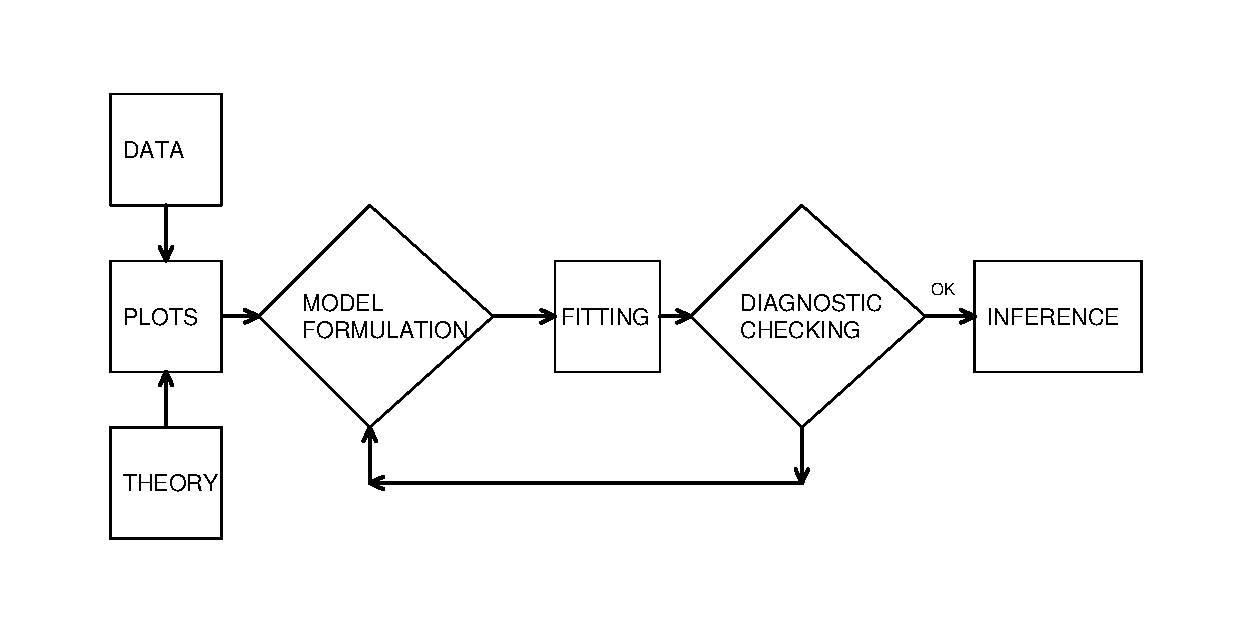
\includegraphics[width=1\textwidth]{Chapter5/F5Iterative.eps}
   \caption{\label{F5:Iterative} \small The iterative model specification process.}
\end{figure}

\newpage

\marginparjed{Diagnostic checking reveals symptoms of mistakes made
in previous specification steps and provides ways to correct these
mistakes.}\index{diagnostic checking!data
criticism}\index{diagnostic checking!model criticism}


This iterative process provides a useful recipe for structuring the
task of specifying a model to represent a set of data. The first
step, the model formulation stage, is accomplished by examining the
data graphically and using prior knowledge of relationships, such as
from economic theory or standard industry practice. The second step
in the iteration is based on the assumptions of the specified model.
These assumptions must be consistent with the data to make valid use
of the model. The third step, \emph{diagnostic checking}, is also
known as \emph{data and model criticism}; the data and model must be
consistent with one another before additional inferences can be
made. Diagnostic checking is an important part of the model
formulation; it can reveal mistakes made in previous steps and
provide ways to correct these mistakes.

The iterative process also emphasizes the skills you need to make
regression analysis work. First, you need a willingness to summarize
information numerically and portray this information graphically.
Second, it is important to develop an understanding of model
properties. You should understand how a theoretical model behaves in
order to match a set of data to it. Third, understanding theoretical
properties of the model are also important for inferring general
relationships based on the behavior of the data.


\section{Automatic Variable Selection
Procedures}\label{S5:Automatic}

Business and economics relationships are complicated; there are
typically many variables that could serve as useful predictors of
the dependent variable. In searching for a suitable relationship,
there is a large number of potential models that are based on linear
combinations of explanatory variables and an infinite number that
can be formed from nonlinear combinations. To search among models
based on linear combinations, several automatic procedures are
available to select variables to be included in the model. These
automatic procedures are easy to use and will suggest one or more
models that you can explore in further detail.

To illustrate how large is the potential number of linear models,
suppose that there are only four variables, $x_{1},$ $x_2,$ $x_3$
and $x_4$, under consideration for fitting a model to $y$. Without
any consideration of multiplication or other nonlinear combinations
of explanatory variables, how many possible models are there? Table
\ref{T5:NumberModels} shows that the answer is 16.

\begin{table}[h]
\scalefont{0.9}

\caption{\label{T5:NumberModels} Sixteen Possible Models}
\begin{tabular}{llll}
\hline
E $y=\beta_0$ &  &  & 1 model with no independent \\
&  &  & \ \ variables \\
E $y=\beta_0+\beta_1x_i,$ & $i=$ & $1,2,3,4$ & 4 models with one
independent \\
&  &  & \ \ variable \\
E $y = \beta_0 + \beta_1 x_i + \beta_2 x_j,$ & $(i,j)=$ & $
(1,2),(1,3),(1,4),$ & 6 models with two independent \\
&  & $(2,3),(2,4),(3,4)$ & \ \ variables \\
E $y = \beta_0 + \beta_1 x_1 + \beta_2 x_j$ & $(i,j,k)=$ & $
(1,2,3),(1,2,4),$ & 4 models with three independent \\
$\ \ \ \ \ \ \ \ +\beta_3x_{k},$ &  & $(1,3,4),(2,3,4)$ & \ \
variables
\\
E $y = \beta_0 + \beta_1 x_1 + \beta_2 x_2$ &  &  & 1 model with all
independent \\
$\ \ \ \ \ \ \ \ +\beta_3 x_3 + \beta_4 x_4$ &  &  & \ \ variables \\
\hline
\end{tabular}
\scalefont{1.1111}
\end{table}


\noindent If there were only three explanatory variables, then you
can use the same logic to verify that there are eight possible
models. Extrapolating from these two examples, how many linear
models will there be if there are ten explanatory variables? The
answer is 1,024, which is quite a few. In general, the answer is
$2^k$, where $k$ is the number of explanatory variables. For
example, $2^3$ is 8, $2^4$ is 16, and so on.

In any case, for a moderately large number of explanatory variables,
there are many potential models that are based on linear
combinations of explanatory variables. We would like a procedure to
search quickly through these potential models to give us more time
to think about other interesting aspects of model selection.
\textit{Stepwise regression} are procedures that employ
\textit{t}-tests to check the ``significance'' of explanatory
variables entered into, or deleted from, the model.

To begin, in the \emph{forward selection} version of stepwise
regression, variables are added one at a time. In the first stage,
out of all the candidate variables the one that is most
statistically significant is added to the model. At the next stage,
with the first stage variable already included, the next most
statistically significant variable is added. This procedure is
repeated until all statistically significant variables have been
added. Here, statistical significance is typically assessed using a
variable's $t$-ratio -- the cut-off for statistical significance is
typically a pre-determined $t$-value (such as two, corresponding to
an approximate 95\% significance level).\index{variable
selection!forwards stepwise regression}

The \emph{backwards selection} version works in a similar manner,
except that all variables are included in the initial stage and then
are dropped one at a time (instead of added).\index{variable
selection!backwards stepwise regression}

More generally, an algorithm that adds and deletes variables at each
stage is sometimes known as \emph{the} stepwise regression
algorithm.\index{variable selection!stepwise regression}



\bigskip

\boxedjed
\subsubsection*{Stepwise Regression Algorithm}

Suppose that the analyst has identified one variable as the
response, $y$, and $k$ potential explanatory variables, $x_1, x_2,
\ldots, x_k$.
\begin{enumerate}

\item Consider all possible regressions using one explanatory variable.
For each of the $k$ regressions, compute $t(b_1)$, the $t$-ratio for
the slope. Choose that variable with the largest $t$-ratio. If the
\textit{t}-ratio does not exceed a pre-specified $t$-value (such as
two), then do not choose any variables and halt the procedure.

\item Add a variable to the model from the previous step. The variable to enter
is the one that makes the largest significant contribution. To
determine the
size of contribution, use the absolute value of the variable's \textit{t}%
-ratio. To enter, the $t$-ratio must exceed a specified $t$-value in
absolute value.

\item Delete a variable to the model from the previous step. The variable to be
removed is the one that makes the smallest contribution. To
determine the size of contribution, use the absolute value of the
variable's $t$-ratio. To be removed, the $t$-ratio must be less than
a specified $t$-value in absolute value.

\item Repeat steps (ii) and (iii) until all possible additions and deletions are
performed.
\end{enumerate}

\end{boxedminipage}

\bigskip


\noindent When implementing this routine, some statistical software
packages use an \textit{F-}test in lieu of $t$-tests. Recall, when
only one variable is being considered, that ($t$-ratio)$^{2}$ =
\textit{F-}ratio and thus these procedures are equivalent.

This algorithm is useful in that it quickly searches through a number of
candidate models. However, there are several drawbacks:
\begin{enumerate}

\item The procedure ``snoops'' through a large number of models and may
fit the data ``too well.''

\item There is no guarantee that the selected model is the best. The algorithm
does not consider models that are based on nonlinear combinations of
explanatory variables. It also ignores the presence of outliers and
high leverage points. \index{leverage}\index{residual!outlier}

  \item In addition, the algorithm does not even search all $2^{k}$ possible
linear regressions.

  \item The algorithm uses one criterion, a \textit{t}-ratio, and does not
consider other criteria such as $s$, $R^2$, $R_a^2$, and so on.

  \item There is a sequence of significance tests involved. Thus, the
significance level that determines the \textit{t}-value is not
meaningful.

  \item By considering each variable separately, the algorithm does not take into
account the joint effect of explanatory variables.

  \item Purely automatic procedures may not take into account an investigator's
special knowledge.

\end{enumerate}


Many of the criticisms of the basic stepwise regression algorithm
can be addressed with modern computing software that is now widely
available. We now consider each drawback, in reverse order. To
respond to drawback number (vii), many statistical software routines
have options for forcing variables into a model equation. In this
way, if other evidence indicates that one or more variables should
be included in the model, then the investigator can force the
inclusion of these variables.

For drawback number (vi), in Section \ref{S5:Suppressor} on
\textit{suppressor variables}, we will provide examples of variables
that do not have important individual effects but are important when
considered jointly. These combinations of variables may not be
detected with the basic algorithm but will be detected with the
backwards selection algorithm. Because the backwards procedure
starts with all variables, it will detect, and retain, variables
that are jointly important.\index{explanatory variable!suppressor}

Drawback number (v) is really a suggestion about the way to use
stepwise regression. Bendel and Afifi (1977) suggested using a
cut-off smaller than you ordinarily might. For example, in lieu of
using \textit{t}-value = 2 corresponding approximately to a 5\%
significance level, consider using \textit{t}-value = 1.645
corresponding approximately to a 10\% significance level. In this
way, there is less chance of screening out variables that may be
important. A lower bound, but still a good choice for exploratory
work, is a cut-off as small as \textit{t}-value = 1. This choice is
motivated by an algebraic result: when a variable enters a model,
$s$ will decrease if the \textit{t}-ratio exceeds one in absolute
value.

\marginparjed{When a variable enters a model, $s$ will decrease if
the \textit{t}-ratio exceeds one in absolute value.}

To address drawbacks number (iii) and (iv), we now introduce the \textit{%
best regressions }routine. Best regressions is a useful algorithm that is
now widely available in statistical software packages. The best regression
algorithm searches over all possible combinations of explanatory variables,
unlike stepwise regression, that adds and deletes one variable at a time.
For example, suppose that there are four possible explanatory variables, $%
x_1$, $x_2$, $x_3$ and $x_4$, and the user would like to know what
is the best two variable model. The best regression algorithm
searches over all six models of the form E $y$ = $\beta_0$ +
$\beta_1$ $x_i$ + $\beta_2$ $x_j$. Typically, a best regression
routine recommends one or two models for each $p$ coefficient model,
where \textit{p} is a number that is user specified. Because it has
specified the number of coefficients to enter the model, it does not
matter which of the criteria we use: $R^2$, $R_a^2$, or
$s$.\index{variable selection!best regressions}

The best regression algorithm performs its search by a clever use of
the algebraic fact that, when a variable is added to the model, the
error sum of squares does not increase. Because of this fact,
certain combinations of variables included in the model need not be
computed. An important drawback of this algorithm is that it can
take a considerable amount of time when the number of variables
considered is large.

Users of regression do not always appreciate the depth of drawback
number (i), \textit{data-snooping}. Data-snooping occurs when the
analyst fits a great number of models to a data set. We will address
the problem of data-snooping in Section \ref{S5:ModelValidation} on
model validation. Here, we illustrate the effect of data-snooping in
stepwise regression.

\linejed\index{examples!data snooping in stepwise regression}

\textbf{Example: Data-Snooping in Stepwise
Regression.}\ecaptionjed{Data-Snooping in Stepwise Regression} The
idea of this illustration is due to Rencher and Pun (1980). Consider
$n=100$ observations of $y$ and fifty explanatory variables, $x_1,
x_2, \ldots,x_{50}$. The data we consider here were simulated using
independent standard normal random variates. Because the variables
were simulated independently, we are working under the null
hypothesis of no relation between the response and the explanatory
variables, that is, H$_0$: $\beta_1=\beta_2=$ $\ldots$
$=\beta_{50}=0$. Indeed, when the model with all
fifty explanatory variables was fit, it turns out that $s=1.142$, $%
R^2=46.2\%$ and \textit{F-}ratio = $(Regression~MS) / (Error~MS)$ =
0.84. Using an \textit{F-}distribution with $df_1=50$ and $df_2=49$,
the 95th percentile is 1.604. In fact, 0.84 is the 27th percentile
of this distribution, indicating that the \textit{p-}value is 0.73.
Thus, as expected, the data are in congruence with $H_0$.

Next, a stepwise regression with \textit{t}-value = 2 was performed. Two
variables were retained by this procedure, yielding a model with $s=1.05$, $%
R^2=9.5\%$ and \textit{F-}ratio = 5.09. For an
\textit{F-}distribution with $df_1=2$ and $df_2=97$, the 95th
percentile is \textit{F-}value = 3.09. This indicates that the two
variables are statistically significant predictors of $y$. At first
glance, this result is surprising. The data were generated so
that $y$ is unrelated to the explanatory variables. However, because \textit{%
F-}ratio $>$ \textit{F-}value, the \textit{F-}test indicates that
two explanatory variables are significantly related to $y$. The
reason is that stepwise regression has performed many hypothesis
tests on the data. For example, in Step 1, fifty tests were
performed to find significant variables. Recall that a 5\% level
means that we expect to make roughly one mistake in 20. Thus, with
fifty tests, we expect to find $50(0.05)=2.5$ ``significant''
variables, even under the null hypothesis of no relationship between
$y$ and the explanatory variables.

To continue, a stepwise regression with \textit{t-}value = 1.645 was
performed. Six variables were retained by this procedure, yielding a
model with $s=0.99$, $R^2=22.9\%$ and \textit{F-}ratio = 4.61. As
before, an \textit{F-}test indicates a significant relationship
between the response and these six explanatory variables.

\marginparjed{When explanatory variables are selected using the
data, \textit{t-}ratios and \textit{F-}ratios will be too large,
thus overstating the importance of variables in the model.}

To summarize, using simulation we constructed a data set so that the
explanatory variables have no relationship with the response.
However, when using stepwise regression to examine the data, we
``found'' seemingly significant relationships between the response
and certain subsets of the explanatory variables. This example
illustrates a general caveat in model selection: when explanatory
variables are selected using the data, \textit{t-}ratios and
\textit{F-}ratios will be too large, thus overstating the importance
of variables in the model.

\linejed

\newpage

\marginparjed{A model suggested by automatic variable selection
procedures should be subject to the same careful diagnostic checking
procedures as a model arrived at by any other means.}

Stepwise regression and best regressions are examples of
\textit{automatic variable selection procedures}. In your modeling
work, you will find these procedures to be useful because they can
quickly search through several candidate models. However, these
procedures do ignore nonlinear alternatives as well as the effect of
outliers and high leverage points. The main point of the procedures
is to mechanize certain routine tasks. This automatic selection
approach can be extended and indeed, there are a number of so-called
``expert systems'' available in the market. For example, algorithms
are available that ``automatically'' handle unusual points such as
outliers and high leverage points. A model suggested by automatic
variable selection procedures should be subject to the same careful
diagnostic checking procedures as a model arrived at by any other
means.

\section{Residual Analysis}\label{S5:ResidualAnalysis}
\index{diagnostic checking!residual analysis}

Recall the role of a residual in the linear regression model
introduced in Section 2.6. A residual is a response minus the
corresponding fitted value under the model. Because the model
summarizes the linear effect of several explanatory variables, we
may think of a residual as a response controlled for values of the
explanatory variables. If the model is an adequate representation of
the data, then residuals should closely approximate random errors.
Random errors are used to represent the natural variation in the
model; they represent the result of an unpredictable mechanism.
Thus, to the extent that residuals resemble random errors, there
should be no discernible patterns in the residuals. Patterns in the
residuals indicate the presence of additional information that we
hope to incorporate into the model. A lack of patterns in the
residuals indicates that the model seems to account for the primary
relationships in the data.

\marginparjed{Patterns in the residuals indicate the presence of
additional information that we hope to incorporate into the model. A
lack of patterns in the residuals indicates that the model seems to
account for the primary relationships in the data.}

\subsection{Residuals}\label{S5:Residuals}\index{residual}

There are at least four types of patterns that can be uncovered
through the residual analysis. In this section, we discuss the first
two; residuals that are unusual and those that are related to other
explanatory variables. We then introduce the third type, residuals
that display a heteroscedastic pattern, in Section
\ref{S5:Heteroscedasticity}. In our study of time series data that
begins in Chapter 7, we will introduce the fourth type, residuals
that display patterns through
time.\index{heteroscedasticity}\index{residual!standardized}

When examining residuals, it is usually easier to work with a
\textit{standardized residual}, a residual that has been rescaled to
be dimensionless. We generally work with standardized residuals
because we achieve some carry-over of experience from one data set
to another and may thus focus on relationships of interest. By using
standardized residuals, we can train ourselves to look at a variety
of residual plots and immediately recognize an unusual point when
working in standard units.

There are a number of ways of defining a standardized residual.
Using $e_i = y_i-\hat{y}_i$ as the $i$th residual, here are three
commonly used definitions:

\begin{equation} \label{E5:StdResid}
\text{(a) }\frac{e_i}{s},\text{ \ \ \ (b) }\frac{e_i}{s\sqrt{
1-h_{ii}}}, \text { \  \   \   }\text{(c)
}\frac{e_i}{s_{(i)}\sqrt{1-h_{ii}}}\text{\ }.
\end{equation}
\index{leverage} \noindent Here, $h_{ii}$ is the $i$th leverage. It
is calculated based on values of the explanatory variables and will
be defined in Section \ref{S5:Leverage}. Recall that $s$ is the
residual standard deviation (defined in equation 3.8). Similarly,
define $s_{(i)}$ to be the residual standard deviation when running
a regression after having deleted the $i$th observation.

Now, the first definition in (a) is simple and easy to explain. An
easy calculation shows that the sample standard deviation of the
residuals is approximately $s$ (one reason that $s$ is often
referred to as the residual standard deviation). Thus, it seems
reasonable to standardize residuals by dividing by $s$.

The second choice presented in (b), although more complex, is more
precise. The variance of the $i$th residual is
\begin{equation*}
\mathrm{Var}(e_i)=\sigma ^2(1-h_{ii}).
\end{equation*}
This result will be established in equation (\ref{E5:VarResiduals})
of Section \ref{S5:TechSupps}. Note that this variance is smaller
than the variance of the error term, Var $(\varepsilon_i)=\sigma
^2$. Now, we can replace $\sigma $ by its estimate, $s$. Then, this
result leads to using the quantity $s(1-h_{ii})^{1/2}$ as an
estimated standard deviation, or standard error, for $e_i$. Thus, we
define the standard error of $e_i$ to be
\begin{equation*}
se(e_i)=s \sqrt{1-h_{ii}}.
\end{equation*}
Following the conventions introduced in Section 2.6, in this text we
use $e_i/se(e_i)$ to be our \textit{standardized residual}.

\index{residual!studentized}

The third choice presented in (c) is a modification of (b) and is
known as a \textit{studentized residual}. As emphasized in Section
\ref{S5:ResidualsOutliers}, one important use of residuals is to
identify unusually large responses. Now, suppose that the $i$th
response is unusually large and that this is measured through its
residual. This unusually large residual will also cause the value of
$s$ to be large. Because the large effect appears in both the
numerator and denominator, the standardized residual may not detect
this unusual response. However, this large response will not inflate
$s_{(i)}$ because it is constructed after having deleted the $i$th
observation. Thus, when using studentized residuals we get a better
measure of observations that have unusually large residuals. By
omitting this observation from the estimate of $\sigma $, the size
of the observation affects only the numerator $e_i$ and not the
denominator $s_{(i)}$.

As another advantage, studentized residuals follow a
\textit{t-}distribution with $n-(k+1)$ degrees of freedom, assuming
the errors are normally distributed (assumption E5). This knowledge
of the precise distribution helps us assess the degree of model fit,
and is particularly useful in small samples. It is this relationship
with the ``Student's'' \textit{t-}distribution that suggests the
name ``studentized'' residuals.

\subsection{Using Residuals to Identify
Outliers}\label{S5:ResidualsOutliers}\index{residual!outlier}

\marginparjed{A commonly used rule of thumb is to mark an
observation as an outlier if its' standardized residual exceeds two
in absolute value.}

One important role of residual analysis is to identify outliers. An
outlier is an observation that is not well fit by the model; these
are observations where the residual is unusually large. A rule of
thumb that is used by many statistical packages is that an
observation is marked as an outlier if the standardized residual
exceeds two in absolute value. To the extent that the distribution
of standardized residuals mimics the standard normal curve, we
expect about only one in 20 observations, or 95\%, to exceed two in
absolute value and very few observations to exceed three.

Outliers provide a signal that an observation should be investigated
to understand special causes associated with this point. An outlier
is an observation that seems unusual with respect to the rest of the
data set. It is often the case that the reason for this atypical
behavior may be uncovered after additional investigation. Indeed,
this may be the primary purpose of the regression analysis of a data
set.

Consider a simple example of so-called \textit{performance
analysis}. Suppose we have available a sample of $n$ salespeople and
are trying to understand each person's second-year sales based on
their first-year sales. To a certain extent, we expect that higher
first-year sales are associated with higher second-year sales. High
sales may be due to a salesperson's natural ability, ambition, good
territory, and so on. First-year sales may be thought of as a proxy
variable that summarizes these factors. We expect variation in sales
performance both cross-sectionally and across years. It is
interesting when one salesperson performs unusually well (or poorly)
in the second year compared to their first-year performance.
Residuals provide a formal mechanism for evaluating second-year
sales after controlling for the effects of first-year sales.

There are a number of options available for handling outliers.

\bigskip

\boxedjed

\textit{Options for Handling Outliers}
\begin{itemize}
\item  Include the observation in
the usual summary statistics but comment on its effects. An outlier
may be large but not so large as to skew the results of the entire
analysis. If no special causes for this unusual observation can be
determined, then this observation may simply reflect the variability
in the data.

\item  Delete the observation from the data set. The observation may be
determined to be unrepresentative of the population from which the
sample is drawn. If this is the case, then there may be little
information contained in the observation that can be used to make
general statements about the population. This option means that we
would omit the observation from the regression summary statistics
and discuss it in our report as a separate case.

\item  Create a binary variable to indicate the presence of an outlier. If one or several
special causes have been identified to explain an outlier, then
these causes could be introduced into the modeling procedure
formally by introducing a variable to indicate the presence (or
absence) of these causes. This approach is similar to point deletion
but allows the outlier to be formally included in the model
formulation so that, if additional observations arise that are
affected by the same causes, then they can be handled on an
automatic basis.

\end{itemize}

\end{boxedminipage}

\bigskip

\subsection{Using Residuals to Select Explanatory
Variables}\label{S5:ResidualsExplanatory}

Another important role of residual analysis is to help identify
additional explanatory variables that may be used to improve the
formulation of the model. If we have specified the model correctly,
then residuals should resemble random errors and contain no
discernible patterns. Thus, when comparing residuals to explanatory
variables, we do not expect any relationships. If we do detect a
relationship, then this suggests the need to control for this
additional variable. This can be accomplished by introducing the
additional variable into the regression model.

Relationships between residuals and explanatory variables can be
quickly established using correlation statistics. However, if an
explanatory variable is already included in the regression model,
then the correlation between the residuals and an explanatory
variable will be zero (Section \ref{S5:ProjMatrix} provides the
algebraic demonstration). It is a good idea to reinforce this
correlation with a scatter plot. Not only will a plot of residuals
versus explanatory variables reinforce graphically the correlation
statistic, it will also serve to detect potential nonlinear
relationships. For example, a quadratic relationship can be detected
using a scatter plot, not a correlation statistic.

If you detect a relationship between the residuals from a
preliminary model fit and an additional explanatory variable, then
introducing this additional variable will not always improve your
model specification. The reason is that the additional variable may
be linearly related to the variables that are already in the model.
If you would like a guarantee that adding an additional variable
will improve your model, then construct an added variable plot (from
Section 3.4.3). \index{plots!added variable}

To summarize, after a preliminary model fit, you should:
\begin{itemize}
\item Calculate summary statistics and display the distribution of
(standardized) residuals to identify outliers.

\item  Calculate the correlation between the (standardized) residuals and
additional explanatory variables to search for linear relationships.

\item  Create scatter plots between the (standardized) residuals and additional
explanatory variables to search for nonlinear relationships.
\end{itemize}

\linejed

\empexjed{Liquidity}\index{datasets!stock market liquidity}

\textbf{Example: Stock Market Liquidity.}\ecaptionjed{Stock
Liquidity} An investor's decision to purchase a stock is generally
made with a number of criteria in mind. First, investors usually
look for a high expected return. A second criterion is the riskiness
of a stock which can be measured through the variability of the
returns. Third, many investors are concerned with the length of time
that they are committing their capital with the purchase of a
security. Many income stocks, such as utilities, regularly return
portions of capital investments in the form of dividends. Other
stocks, particularly growth stocks, return nothing until the sale of
the security. Thus, the average length of investment in a security
is another criterion. Fourth, investors are concerned with the
ability to sell the stock at any time convenient to the investor. We
refer to this fourth criterion as the \textit{liquidity }of the
stock. The more liquid is the stock, the easier it is to sell. To
measure the liquidity, in this study we use the number of shares
traded on an exchange over a specified period of time (called the
VOLUME). We are interested in studying the relationship between the
volume and other financial characteristics of a
stock.\index{actuarial \& financial terms and concepts!stock
liquidity}

We begin this study with 126 companies whose options were traded on December
3, 1984. The stock data were obtained from Francis Emory Fitch, Inc. for the
period from December 3, 1984 to February 28, 1985. For the trading activity
variables, we examine
\begin{itemize}
\item the three months total trading volume (VOLUME, in millions of shares),
\item the three months total number of transactions (NTRAN), and
\item the average time between transactions (AVGT, measured in minutes).
\end{itemize}
\noindent For the firm size variables, we use the
\begin{itemize}
\item opening stock price on January 2, 1985 (PRICE),
\item  the number of outstanding shares on December 31, 1984 (SHARE, in millions of shares), and
\item  the market equity value (VALUE, in billions of dollars) obtained by taking the product of PRICE and SHARE.
\end{itemize}
\noindent Finally, for the financial leverage, we examine the
debt-to-equity ratio (DEB\_EQ) obtained from the Compustat
Industrial Tape and the Moody's manual. The data in SHARE are
obtained from the Center for Research in Security Prices (CRSP)
monthly tape.\index{actuarial \& financial terms and
concepts!financial leverage}

After examining some preliminary summary statistics of the data,
three companies were deleted because they either had an unusually
large volume or high price. They are Teledyne and Capital Cities
Communication, whose prices were more than four times the average
price of the remaining companies, and American Telephone and
Telegraph, whose total volume was more than seven times than the
average total volume of the remaining companies. Based on additional
investigation, the details of which are not presented here, these
companies were deleted because they seemed to represent special
circumstances that we would not wish to model. Table
\ref{T5:LiquidSumStats} summarizes the descriptive statistics based
on the remaining $n=123$ companies. For example, from Table
\ref{T5:LiquidSumStats} we see that the average time between
transactions is about five minutes and this time ranges from a
minimum of less than a minute to a maximum of about 20 minutes.

\begin{table}[h]
\scalefont{0.9}

\caption{\label{T5:LiquidSumStats} Summary Statistics of the Stock
Liquidity Variables}

\begin{tabular}{lrrrrr}
\hline
&  & & Standard &  &  \\
& Mean & Median & deviation & Minimum & Maximum \\
\hline VOLUME & 13.423 & 11.556 & 10.632 &
0.658 & 64.572 \\
AVGT & 5.441 & 4.284 & 3.853 & 0.590 &
20.772 \\
NTRAN & 6436 & 5071 & 5310 & 999 &
36420 \\
PRICE & 38.80 & 34.37 & 21.37 & 9.12 &
122.37 \\
SHARE & 94.7 & 53.8 & 115.1 & 6.7 &
783.1 \\
VALUE & 4.116 & 2.065 & 8.157 & 0.115 &
75.437 \\
DEB\_EQ & 2.697 & 1.105 & 6.509 & 0.185 & 53.628 \\ \hline
\end{tabular}

\textit{Source: Francis Emory Fitch, Inc., Standard \& Poor's
Compustat, and University of Chicago's Center for Research on
Security Prices.}

\scalefont{1.1111}
\end{table}

Table \ref{T5:LiquidCorr} reports the correlation coefficients and
Figure \ref{F5:LiquidPlot} provides the corresponding scatterplot
matrix. If you have a background in finance, you will find it
interesting to note that the financial leverage, measured by
DEB\_EQ, does not seem to be related to the other variables. From
the scatterplot and correlation matrix, we see a strong relationship
between VOLUME and the size of the firm as measured by SHARE and
VALUE. Further, the three trading activity variables, VOLUME, AVGT
and NTRAN, are all highly related to one another.

\begin{table}[h]
\scalefont{0.9}

\caption{\label{T5:LiquidCorr} Correlation Matrix of the Stock
Liquidity}
\begin{tabular}{lrrrrrrr}
\hline & AVGT & NTRAN & PRICE & SHARE & VALUE & DEB\_EQ \\ \hline
\multicolumn{1}{l}{NTRAN} & $-0.668$ &  &  &  &  &  \\
\multicolumn{1}{l}{PRICE} & $-0.128$ & $0.190$ &  &  &  &  \\
\multicolumn{1}{l}{SHARE} & $-0.429$ & $0.817$ & $0.177$ &  &  &  \\
\multicolumn{1}{l}{VALUE} & $-0.318$ & $0.760$ & $0.457$ & $0.829$ &  &  \\
\multicolumn{1}{l}{DEB\_EQ} & $0.094$ & $-0.092$ & $-0.038$ & $-0.077$ & $%
-0.077$ &  \\
\multicolumn{1}{l}{VOLUME} & $-0.674$ & $0.913$ & $0.168$ & $0.773$ & $0.702$
& $-0.052$ \\ \hline
\end{tabular}
\scalefont{1.1111}
\end{table}

Figure \ref{F5:LiquidPlot} shows that the variable AVGT is inversely
related to VOLUME and NTRAN is inversely related to AVGT. In fact,
it turned out the correlation between the average time between
transactions and the reciprocal of the number of transactions was
$99.98\%$! This is not so surprising when one thinks about how AVGT
might be calculated. For example, on the New York Stock Exchange,
the market is open from 10:00 A.M. to 4:00 P.M. For each stock on a
particular day, the average time between transactions times the
number of transactions is nearly equal to 360 minutes (= 6 hours).
Thus, except for rounding errors because transactions are only
recorded to the nearest minute, there is a perfect linear
relationship between AVGT and the reciprocal of NTRAN.


\begin{figure}[htp]
  \begin{center}
    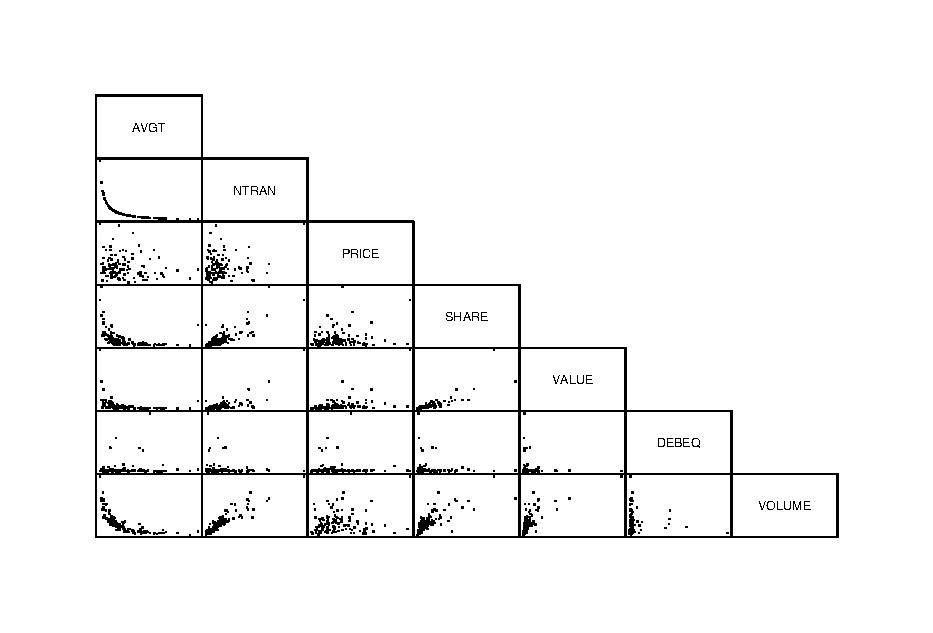
\includegraphics[width=1\textwidth]{Chapter5/F5LiquidPlot.eps}
    \caption{\label{F5:LiquidPlot} \small  Scatterplot matrix for
stock liquidity variables. The number of transactions variable
(NTRAN) appears to be strongly related to the VOLUME of shares
traded, and inversely related to AVGT.}
  \end{center}
\end{figure}


To begin to understand the liquidity measure VOLUME, we first fit a
regression model using NTRAN as an explanatory variable. The fitted
regression model is:

\scalefont{0.9}
\begin{center}
\begin{tabular}{lccl}
  VOLUME & = & 1.65 & +0.00183 NTRAN \\
  std errors &  & (0.0018)  & (0.000074) \\
\end{tabular}
\end{center}
\scalefont{1.1111}

\noindent with $R^2=83.4\%$ and $s=4.35$. Note that the
\textit{t-}ratio for the slope associated with NTRAN is
$t(b_1)=b_1/se(b_1)=0.00183/0.000074=24.7$, indicating strong
statistical significance. Residuals were computed using this
estimated model. To see if the residuals are related to the other
explanatory variables, below is a table of correlations.


\begin{table}[h]
\scalefont{0.9}

\caption{\label{T5:LiquidResidCorr1} First Table of Correlations }
\begin{tabular}{cccccc}
 \hline
& AVGT & PRICE & SHARE & VALUE & DEB\_EQ \\
RESID & -0.155 & -0.017 & 0.055 & 0.007 & 0.078 \\ \hline
\end{tabular}

{\small \textit{Note:} The residuals were created from a regression
of VOLUME on NTRAN.} \scalefont{1.1111}
\end{table}

The correlation between the residual and AVGT and the scatter plot (not
given here) indicates that there may be some information in the variable
AVGT in the residual. Thus, it seems sensible to use AVGT directly in the
regression model. Remember that we are interpreting the residual as the
value of VOLUME having controlled for the effect of NTRAN.

We next fit a regression model using NTRAN and AVGT as an explanatory
variables. The fitted regression model is:

\scalefont{0.9}
\begin{center}
\begin{tabular}{lccll}
  VOLUME     & = & 4.41   & -0.322 AVGT & +0.00167 NTRAN \\
  std errors &   & (1.30) & (0.135)     & (0.000098)     \\
\end{tabular}
\end{center}
\scalefont{1.1111}


\noindent with $R^2=84.2\%$ and $s=4.26$. Based on the
\textit{t-}ratio for AVGT, $t(b_{AVGT})=$ $(-0.322)/0.135$ $=-2.39$,
it seems as if AVGT is a useful explanatory variable in the model.
Note also that $s$ has decreased, indicating that $R_a^2$ has
increased.

Table \ref{T5:LiquidResidCorr2} provides correlations between the
model residuals and other potential explanatory variables and
indicates that there does not seem to be much additional information
in the explanatory variables. This is reaffirmed by the
corresponding table of scatter plots in Figure
\ref{F5:LiquidResidPlot}. The histograms in Figure
\ref{F5:LiquidResidPlot} suggest that although the distribution of
the residuals is fairly symmetric, the distribution of each
explanatory variable is skewed. Because of this, transformations of
the explanatory variables were explored. This line of thought
provided no real improvements and thus the details are not provided
here.

\begin{figure}[htp]
  \begin{center}
    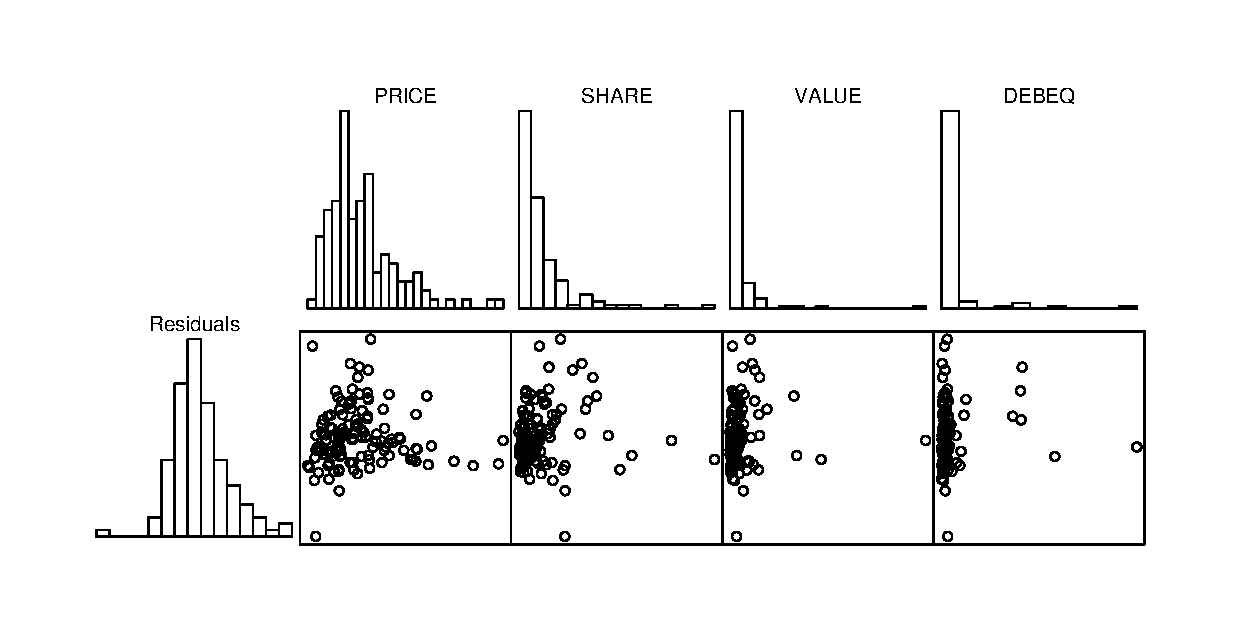
\includegraphics[width=1\textwidth]{Chapter5/F5LiquidResidPlot.eps}
    \caption{\label{F5:LiquidResidPlot} \small  Scatterplot matrix of the
residuals from the regression of VOLUME on NTRAN and AVGT on the
vertical axis and the remaining predictor variables on the
horizontal axes.}
  \end{center}
\end{figure}



\begin{table}[h]
\scalefont{0.9}

\caption{\label{T5:LiquidResidCorr2} Second Table of Correlations }
\begin{tabular}{ccccc}
\hline
& PRICE & SHARE & VALUE & DEB\_EQ \\
RESID & -0.015 & 0.096 & 0.071 & 0.089 \\ \hline
\end{tabular}

{\small \textit{Note:} The residuals were created from a regression
of VOLUME on NTRAN and AVGT.} \scalefont{1.1111} \scalefont{1.1111}
\end{table}

\linejed

\section{Influential Points}

Not all points are created equal -- in this section we will see that
specific observations can potentially have a disproportionate effect
on the overall regression fit. We will call such points
``influential.'' This is not too surprising; we have already seen
that regression coefficients estimates are \emph{weighted} sums of
responses (see Section 3.2.4). Some observations have heavier
weights than others and thus have a greater influence on the
regression coefficient estimates. Of course, simply because an
observation is influential does not mean that it is incorrect or
that its impact on the model is misleading. As analysts, we would
simply like to know whether our fitted model is sensitive to mild
changes such as the removal of a single point so that we feel
comfortable generalizing our results from the sample to a larger
population.

To assess influence, we think of observations as being unusual
responses, given a set of explanatory variables, or having an
unusual set of explanatory variables. We have already seen in
Section \ref{S5:ResidualAnalysis} how to assess unusual responses
using residuals. This section focuses on unusual sets of explanatory
variables.


\subsection{Leverage}\label{S5:Leverage}\index{leverage}

We introduced this topic in Section 2.6 where we called an
observation having an unusual explanatory variable a ``high leverage
point.'' With more than one explanatory variable, determining
whether an observation is a high leverage point is not as
straightforward. For example, it is possible for an observation to
be ``not unusual'' for any single variable and yet still be unusual
in the space of explanatory variables. Consider the fictitious data
set represented in Figure \ref{F5:Ellipsoid}. Visually, it seems
clear that the point marked in the upper right hand corner is
unusual. However, it is not unusual when examining the histogram of
either $x_1$ or $x_2$. It is only unusual when the explanatory
variables are considered jointly.



\begin{figure}[htp]
  \begin{center}
    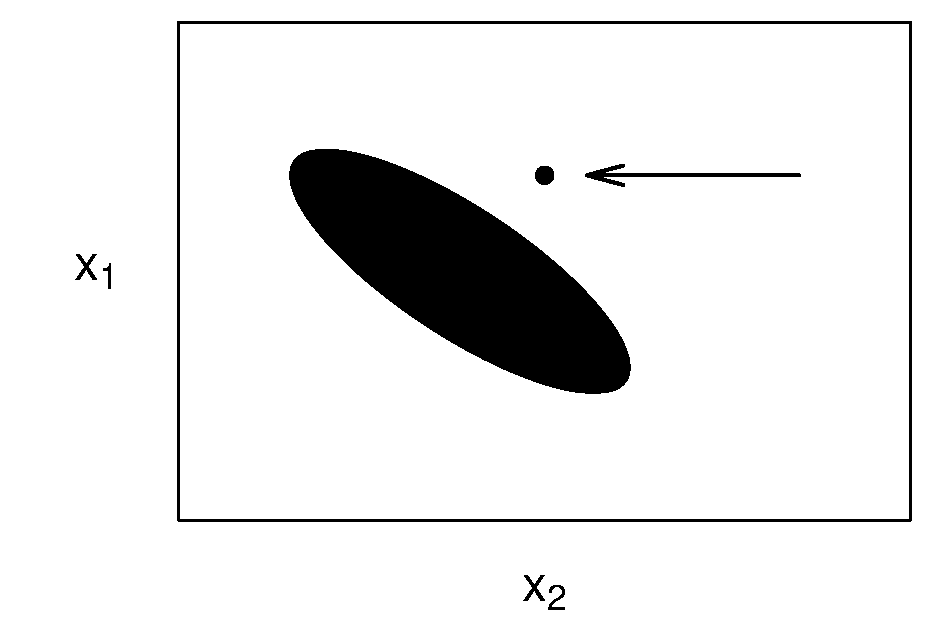
\includegraphics[width=0.5\textwidth]{Chapter5/F5Ellipsoid.eps}
    \caption{\label{F5:Ellipsoid} \small  The ellipsoid
represents most of the data. The arrow marks an unusual point.}
  \end{center}
\end{figure}


For two explanatory variables, this is apparent when examining the
data graphically. Because it is difficult to examine graphically
data having more than two explanatory variables, we need a numerical
procedure for assessing leverage.


To define the concept of leverage in multiple linear regression, we
use some concepts from matrix algebra. Specifically, in Section 3.1,
we showed that the vector of least squares regression coefficients
could be calculated using
$\mathbf{b}=\mathbf{(X}^{\prime}\mathbf{X)}^{-1}\mathbf{X}^{\prime}\mathbf{y
}$. Thus, we can express the vector of fitted values
$\hat{y}=(\hat{y}_1,...,\hat{y}_n)^{\prime}$ as
\begin{equation}\label{E5:FittedValues}
\mathbf{\hat{y}}=\mathbf{Xb}
\end{equation}
Similarly, the vector of residuals is the vector of response minus
the vector of fitted values, that is,
$\mathbf{e}=\mathbf{y-\hat{y}}$.

From expression for the regression coefficients \textbf{b} in
equation (3.4), we have $\mathbf{\hat{y}}=
\mathbf{X(X}^{\prime}\mathbf{X)}^{-1}\mathbf{X}^{\prime}\mathbf{y}$.
This equation suggests defining $\mathbf{H} =
\mathbf{X(X}^{\prime}\mathbf{X)}^{-1} \mathbf{X}^{\prime}$, so that
$\mathbf{\hat{y}}=\mathbf{Hy}$. From this,
the matrix $\mathbf{H}$ is said to \textit{project} the vector of responses $%
\mathbf{y}$ onto the vector of fitted values $\mathbf{\hat{y}}$.
Alternatively, you may think of $\mathbf{H}$ as the matrix that puts
the ``hat,'' or carat, on $\mathbf{y}$. From the $i$th row of the
vector equation $\mathbf{\hat{y}=Hy}$, we have
\begin{equation*}
\hat{y}_i=h_{i1}y_1+h_{i2}y_2+...+h_{ii}y_i+...+h_{in}y_{n}.
\end{equation*}\index{symbols!$h_{ii}$, $i$th leverage}
Here, $h_{ij}$ is the number in the $i$th row and $j$th column of
$\mathbf{H} $. From this expression, we see that the larger is
$h_{ii}$, the larger is the effect that the $i$th response $(y_i)$
has on the corresponding fitted value $(\hat{y}_i)$. Thus, we call
$h_{ii}$ to be the \textit{leverage }for the $i$th observation.
Because $h_{ii}$ is the $i$th diagonal element of $\mathbf{H}$, a
direct expression for $h_{ii}$ is
\begin{equation}\label{E5:Leverage}
h_{ii}=\mathbf{x}_i^{\prime}\mathbf{(X}^{\prime}\mathbf{X)}^{-1}\mathbf{x%
}_i
\end{equation} where
$\mathbf{x}_i=(x_{i0},x_{i1},\ldots,x_{ik})^{\prime}$. Because the
values $h_{ii}$ are calculated based on the explanatory variables,
the values of the response variable do not affect the calculation of
leverages.

Large leverage values indicate that an observation may exhibit a
disproportionate effect on the fit, essentially because it is
distant from the other observations (when looking at the space of
explanatory variables). How large is large? Some guidelines are
available from matrix algebra, where we have that
\begin{equation*}
\frac{1}{n}\leq h_{ii}\leq 1
\end{equation*}
and
\begin{equation*}
\bar{h}=\frac{1}{n}\sum_{i=1}^{n}h_{ii}=\frac{k+1}{n}.
\end{equation*}
Thus, each leverage is bounded by $n^{-1}$ and $1$ and the average
leverage equals the number of regression coefficients divided by the
number of observations. From these and related arguments, we use a
widely adopted convention and declare an observation to be a
\textit{high leverage point} if the leverage exceeds three times the
average, that is, if $h_{ii}>3(k+1)/n $.



Having identified high leverage points, as with outliers it is
important for the analyst to search for special causes that may have
produced these unusual points. To illustrate, in Section 2.7 we
identified the 1987 market crash as the reason behind the high
leverage point. Further, high leverage points are often due to
clerical errors in coding the data, which may or may not be easy to
rectify. In general, the options for dealing with high leverage
points are similar to those available for dealing with outliers.
\bigskip

\boxedjed

\emph{Options for Handling High Leverage Points}

\begin{enumerate}

\item Include the observation in the summary statistics but comment on its
effect. For example, an observation may barely exceed a cut-off and its
effect may not be important in the overall analysis.

\item  Delete the observation from the data set. Again, the basic rationale for
this action is that the observation is deemed not representative of
some larger population. An intermediate course of action between (i)
and (ii) is to present the analysis both with and without the high
leverage point. In this way the impact of the point is fully
demonstrated and the reader of your analysis may decide which option
is more appropriate.

\item  Choose another variable to represent the information. In some instances,
another explanatory variables will be available to serve as a
replacement. For example, in an apartment rents example, we could
use the number of bedrooms to replace a square footage variable as a
measure of apartment size. Although an apartment's square footage
may be unusually large causing it to be a high leverage point, it
may have one, two or three bedrooms, depending on the sample
examined.

\item  Use a nonlinear transformation of an explanatory variable. To illustrate, with our Stock Liquidity
example in Section \ref{S5:ResidualsExplanatory}, we can transform
the debt-to-equity DEB\_EQ continuous variable into a variable that
indicates the presence of ``high'' debt-to-equity. For example, we
might code DE\_IND $=1$ if DEB\_EQ $>5$ and DE\_IND $=0$ if DEB\_EQ
$\leq 5$. With this recoding, we still retain information on the
financial leverage of a company without allowing the large values of
DEB\_EQ drive the regression fit.
\end{enumerate}
\end{boxedminipage}
\bigskip


Some analysts use ``robust'' estimation methodologies as an
alternative to least squares estimation. The basic idea of these
techniques is to reduce the effect of any particular observation.
These techniques are useful in reducing the effect of both outliers
and high leverage points. This tactic may be viewed as intermediate
between one extreme procedure, ignoring the effect of unusual
points, and another extreme, giving unusual points full credibility
by deleting them from the data set. The word \textit{robust }is
meant to suggest that these estimation methodologies are ``healthy''
even when attacked by an occasional bad observation (a germ). We
have seen that this is not true for least squares estimation.

\subsection{Cook's Distance}\index{leverage!Cook's distance}

To quantify the influence of a point, a measure that considers both
the response and explanatory variables is \textit{Cook's Distance}.
This distance, $D_i$, is defined as

\begin{eqnarray}\label{E5:CooksD}
D_i &=&\frac{\sum_{j=1}^{n}(\hat{y}_j-\hat{y}_{j(i)})^2}{(k+1)s^2} \\
&=&\left(\frac{e_i}{se(e_i)}\right)^2\frac{h_{ii}}{(k+1)(1-h_{ii})}.
\nonumber
\end{eqnarray}\index{symbols!$D_i$, Cook's distance}

\noindent The first expression provides a definition. Here,
$\hat{y}_{j(i)}$ is the prediction of the $j$th observation,
computed leaving the $i$th observation out of the regression fit. To
measure the impact of the $i$th observation, we compare the fitted
values with and without the $i$th observation. Each difference is
then squared and summed over all observations to summarize the
impact.

The second equation provides another interpretation of the distance
$D_i$. The first part, $(e_i/se(e_i))^2$, is the square of the $i$th
standardized residual. The second part, $h_{ii}/((k+1)(1-h_{ii}))$,
is attributable solely to the leverage. Thus, the distance $D_i$ is
composed of a measure for outliers times a measure for leverage. In
this way, Cook's distance accounts for both the response and
explanatory variables. Section \ref{S5:OmittingVariables}
establishes the validity of equation (\ref{E5:CooksD}).

To get an idea of the expected size of $D_i$ for a point that is not
unusual, recall that we expect the standardized residuals to be
about one and the leverage $h_{ii}$ to be about $(k+1)/n$. Thus, we
anticipate that $D_i$ should be about $1/n$. Another rule of thumb
is to compare $D_i$ to an \textit{F-}distribution with $df_1=k+1$
and $df_2=n-(k+1)$ degrees of freedom. Values of $D_i$ that are
large compared to this distribution merit attention.

\linejed\index{datasets!outliers and high leverage
points}\index{distributions!F-@{$F-$}}

\textbf{Example: Outliers and High Leverage Points - Continued.} To
illustrate, we return to our example in Section 2.6. In this
example, we considered 19 ``good,'' or base, points plus each of the
three types of unusual points, labeled A, B and C. Table
\ref{T5:Outliers} summarizes the calculations.

\begin{table}[h]
\scalefont{0.9}

\caption{\label{T5:Outliers} Measures of Three Types of Unusual
Points}
\begin{tabular}{cccc}
\hline
& Standardized residual & Leverage & Cook's distance \\
Observation & $e/se(e)$ & $h$ & $D$ \\ \hline
A & 4.00 & .067 & .577 \\
 B & .77 & .550 & .363 \\
C & -4.01 & .550 & 9.832 \\ \hline
\end{tabular}
\scalefont{1.1111}
\end{table}

As noted in Section 2.6, from the standardized residual column we
see that both points A and C are outliers. To judge the size of the
leverages, because there are $n=20$ points, the leverages are
bounded by 0.05 and 1.00 with the average leverage being
$\bar{h}=2/20=0.10$. Using 0.3 ($ = 3 \times  \bar{h}$) as a
cut-off, both points B and C are high leverage points. Note that
their values are the same. This is because, from Figure 2.7, the
values of the explanatory variables are the same and only the
response variable has been changed. The column for Cook's distance
captures both types of unusual behavior. Because the typical value
of $D_i$ is $1/n$ or 0.05, Cook's distance provides one statistic to
alert us to the fact that each point is unusual in one respect or
another. In particular, point C has a very large $D_i$, reflecting
the fact that it is both an outlier and a high leverage point. The
95th percentile of an \textit{F-}distribution with $df_1=2$ and
$df_2=18$ is 3.555. The fact that point C has a value of $D_i$ that
well exceeds this cut-off indicates the substantial influence of
this point.

\linejed

\section{Collinearity}\index{collinearity}

\subsection{What is Collinearity?}

\textit{Collinearity}, or \textit{multicollinearity}, occurs when
one explanatory variable is, or nearly is, a linear combination of
the other explanatory variables. Intuitively, with collinear data it
is useful to think of explanatory variables as being highly
correlated with one another. If an explanatory variable is
collinear, then the question arises as to whether it is redundant,
that is, whether the variable provides little additional information
over and above the information in the other explanatory variables.
The issues are: Is collinearity important? If so, how does it affect
our model fit and how do we detect it? To address the first
question, consider a somewhat pathological example.

\linejed

\textbf{Example: Perfectly Correlated Explanatory Variables.} Joe
Finance was asked to fit the model E
$y=\beta_0+\beta_1x_1+\beta_2x_2$ to a data set. His resulting
fitted model was $\hat{y}=-87+x_1+18x_2.$  The data set under
consideration is:

\scalefont{0.9}
\begin{center}
\begin{tabular}{ccccc}
\hline
$i$ & 1 & 2 & 3 & 4 \\
$y_i$ & 23 & 83 & 63 & 103 \\
$x_{i1}$ & 2 & 8 & 6 & 10 \\
$x_{i2}$ & 6 & 9 & 8 & 10 \\ \hline
\end{tabular}%
\end{center}
\scalefont{1.1111}

Joe checked the fit for each observation. Joe was very happy because
he fit the data perfectly! For example, for the third observation
the fitted value is $\hat{y}_3=-87+6+18(8)=63$, which is equal to
the third response, $y_3 $. Because the response equals the fitted
value, the residual is zero. You may check that this is true of each
observation and thus the $R^2$ turned out to be $100\%$.

However, Jane Actuary came along and fit the model
$\hat{y}=-7+9x_1+2x_2.$ Jane performed the same careful checks that
Joe did and also got a perfect fit ($R^2 = 1)$. Who is right?

The answer is both and neither one. There are, in fact, an infinite
number of fits. This is due to the perfect relationship
$x_2=5+x_1/2$ between the two explanatory variables.

\linejed

This example illustrates some important facts about collinearity.
\bigskip

\boxedjed

\textit{Collinearity Facts}
\begin{itemize}
\item Collinearity neither precludes us from
getting good fits nor from making predictions of new observations.
Note that in the above example we got perfect fits.

\item  Estimates of error variances and, therefore, tests of model adequacy, are
still reliable.

\item  In cases of serious collinearity, standard errors of individual
regression coefficients are larger than cases where, other things
equal, serious collinearity does not exist. With large standard
errors, individual regression coefficients may not be meaningful.
Further, because a large standard error means that the corresponding
\textit{t-}ratio is small, it is difficult to detect the importance
of a variable.
\end{itemize}
\end{boxedminipage}
\bigskip


To detect collinearity, begin with a matrix of correlation
coefficients of the explanatory variables. This matrix is simple to
create, easy to interpret and  quickly captures linear relationships
between pairs of variables. A scatterplot matrix provides a visual
reinforcement of the summary statistics in the correlation matrix.


\subsection{Variance Inflation Factors}\index{symbols!$VIF$, variance inflation
factor}\index{collinearity!variance inflation factor}

Correlation and scatterplot matrices capture only relationships
between pairs of variables. To capture more complex relationships
among several variables, we introduce the \textit{variance inflation
factor (VIF)}. To define a \textit{VIF}, suppose that the set of
explanatory variables is labeled $x_1,x_2,...,x_{k}$. Now, run the
regression using $x_j$ as the ``response'' and the other $x$'s $
(x_1,x_2,...,x_{j-1},x_{j+1},...,x_{k})$ as the explanatory
variables. Denote the coefficient of determination from this
regression by $R_j^2$. We interpret $R_j=\sqrt{R_j^2}$ as the
multiple correlation coefficient between $x_j$ and linear
combinations of the other $x$'s. From this coefficient of
determination, we define the variance inflation factor

\begin{equation*}
VIF_j=\frac{1}{1-R_j^2},\text{ \ \ \ for \ }j=1,2,...,k.
\end{equation*}
A larger $R_j^2$ results in a larger $VIF_j$; this means greater
collinearity between $x_j$ and the other $x$'s. Now, $R_j^2$ alone
is enough to capture the linear relationship of interest. However,
we use $VIF_j$ in lieu of $R_j^2$ as our measure for collinearity
because of the algebraic relationship

\begin{equation} \label{E5:SEsAndVIFs}
se(b_j) = s \frac{\sqrt{VIF_j}}{s_{x_j}\sqrt{n-1}} .
\end{equation}

\noindent Here, $se(b_j)$ and $s$ are standard errors and residual
standard deviation from a full regression fit of $y$ on
$x_1,...,x_{k}$. Further, $s_{x_j} = \sqrt{(n-1)^{-1}
\sum_{i=1}^{n}(x_{ij}-\bar{x}_j)^2 }$ is the sample standard
deviation of the $j$th variable $x_j$. Section
\ref{S5:OmittingVariables} provides a verification of equation
(\ref{E5:SEsAndVIFs}).

Thus, a larger $VIF_j$ results in a larger standard error associated
with the $j$th slope, $b_j$. Recall that $se(b_j)$ is $s$ times the
square root of the $(j+1)$st diagonal element of
$(\mathbf{X^{\prime} X})^{-1}$. The idea is that when collinearity
occurs, the matrix $\mathbf{X^{\prime}X}$ has properties similar to
the number zero. When we attempt to calculate the inverse of
$\mathbf{X^{\prime} X}$, this is analogous to dividing by zero for
scalar numbers. As a rule of thumb, when $VIF_j$ exceeds 10 (which
is equivalent to $R_j^2>90\%$), we say that severe collinearity
exists. This may signal a need for action. \emph{Tolerance}, defined
as the reciprocal of the variance inflation factor, is another
measure of collinearity used by some
analysts.\index{collinearity!tolerance}

\marginparjed{A commonly used rule of thumb is that $VIF_j > 10$ is
a signal that severe collinearity exists.}

For example, with $k=2$ explanatory variables in the model, then
$R_1^2$ is the squared correlation between the two explanatory
variables, say $r_{12}^2$. Then, from equation
(\ref{E5:SEsAndVIFs}), we have that $se(b_j) = s\left( s_{x_j}
\sqrt{n-1} \right)^{-1} \left( 1-r_{12}^2\right)^{-1/2}$, for
$j=1,2$. As the correlation approaches one in absolute value,
$|r_{12}| \rightarrow 1$, then the standard error becomes large
meaning that the corresponding $t$-statistic becomes small. In
summary, a high $VIF$ may mean small $t$-statistics even though
variables are important. Further, one can check that the correlation
between $b_1$ and $b_2$ is $-r_{12}$, indicating that the
coefficient estimates are highly correlated.



\linejed\index{datasets!stock market liquidity}

\textbf{Example: Stock Market Liquidity - Continued.} As an example,
consider a regression of VOLUME on PRICE, SHARE and VALUE. Unlike
the explanatory variables considered in Section
\ref{S5:ResidualsExplanatory}, these three explanatory variables are
not measures of trading activity. From a regression fit, we have
$R^2=61\%$ and $s=6.72$. The statistics associated with the
regression coefficients are in Table \ref{T5:LiquidRegression}.


\begin{table}[h]
\scalefont{0.9}
\caption{\label{T5:LiquidRegression} Statistics from
a Regression of VOLUME on PRICE, SHARE and VALUE}

\begin{tabular}{crrrrr}
\hline
$x_j$ & $s_{x_j}$ & $b_j$ & $se(b_j)$ & $t(b_j)$ & $VIF_j$ \\
\hline PRICE& 21.37 & -0.022 & 0.035&
-0.63& 1.5 \\
SHARE & 115.1 & 0.054 & 0.010 &
5.19 & 3.8 \\
VALUE & 8.157 & 0.313 & 0.162 & 1.94 & 4.7
\\ \hline
\end{tabular}
\scalefont{1.1111}
\end{table}

You may check that the relationship in equation
(\ref{E5:SEsAndVIFs}) is valid for each of the explanatory variables
in Table \ref{T5:LiquidRegression}. Because each $VIF$ statistic is
less than ten, there is little reason to suspect severe
collinearity. This is interesting because you may recall that there
is a perfect relationship between PRICE, SHARE and VALUE in that we
defined the market value to be VALUE = PRICE $\times $ SHARE.
However, the relationship is multiplicative, and hence is nonlinear.
Because the variables are not linearly related, it is valid to enter
all three into the regression model. From a financial perspective,
the variable VALUE is important because it measures the worth of a
firm. From a statistical perspective, the variable VALUE quantifies
the interaction between PRICE and SHARE (interaction variables were
introduced in Section 3.5.3).\index{explanatory
variable!interaction}

\linejed

For collinearity, we are only interested in detecting linear trends,
so nonlinear relationships between variables are not an issue here.
For example, we have seen that it is sometimes useful to retain both
an explanatory variable $(x)$ and its square $(x^2)$, despite the
fact that there is a perfect (nonlinear) relationship between the
two. Still, we must check that nonlinear relationships are not
approximately linear over the sampling region. Even though the
relationship is theoretically nonlinear, if it is close to linear
for our available sample, then problems of collinearity might arise.
Figure \ref{F5:Nearlinear} illustrates this situation.


\begin{figure}[htp]
  \begin{center}
    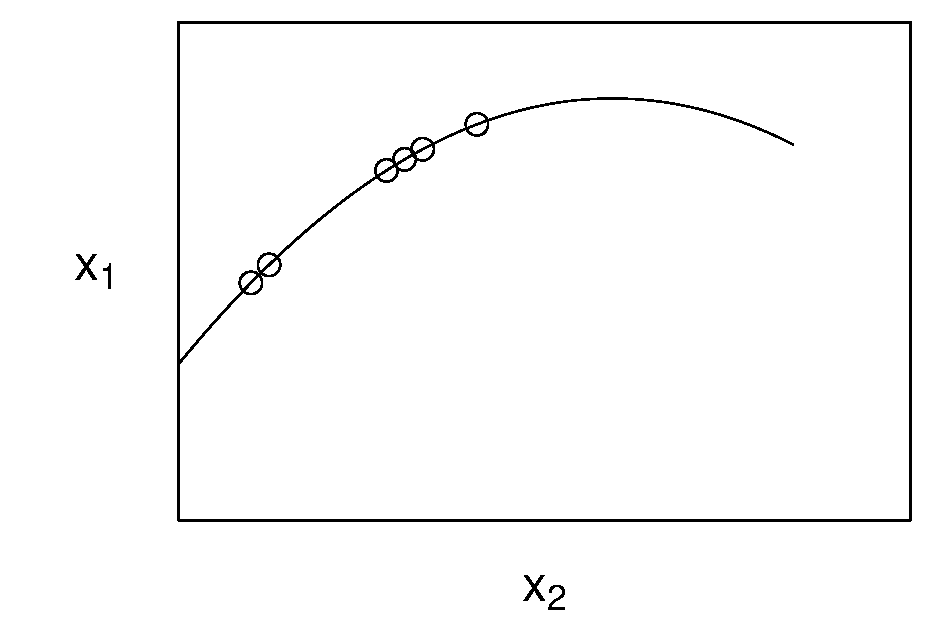
\includegraphics[width=0.5\textwidth]{Chapter5/F5Nearlinear.eps}
    \caption{\label{F5:Nearlinear} \small  The relationship
between $x_1$ and $x_2$ is nonlinear. However, over the region
sampled, the variables have close to a linear relationship.}
  \end{center}
\end{figure}



What can we do in the presence of collinearity? One option is to center each
variable, by subtracting its average and dividing by its standard deviation.
For example, create a new variable $x_{ij}^{\ast }=(x_{ij}-\bar{x}%
_j)/s_{x_j}$ . Occasionally, one variable appears as millions of
units and another variable appears as fractions of units. Compared
to the first mentioned variable, the second variable is close to a
constant column of zeros (in that computers typically retain a
finite number of digits). If this is true, then the second variable
looks very much like a linear shift of the constant column of ones
corresponding to the intercept. This is a problem because, with the
least squares operations, we are implicitly squaring numbers that
can make these columns appear even more similar.

This problem is simply a computational one and is easy to rectify.
Simply recode the variables so that the units are of similar order
of magnitude. Some data analysts automatically center all variables
to avoid these problems. This is a legitimate approach because
regression techniques search for linear relationships; location
 and scale shifts do not affect linear relationships.

Another option is to simply not explicitly account for collinearity in the
analysis but to discuss some of its implications when interpreting the
results of the regression analysis. This approach is probably the most
commonly adopted one. It is a fact of life that, when dealing with business
and economic data, collinearity does tend to exist among variables. Because
the data tends to be observational in lieu of experimental in nature, there
is little that the analyst can do to avoid this situation.

\marginparjed{When severe collinearity exists, often the only option
is to remove one or more variables from the regression equation.}

In the best-case situation, an auxiliary variable that provides
similar information and that eases the collinearity problem, is
available to replace a variable. Similar to our discussion of high
leverage points, a transformed version of the explanatory variable
may also be a useful substitute. In some situations, such an ideal
replacement is not available and we are forced to remove one or more
variables. Deciding which variables to remove is a difficult choice.
When deciding among variables, often the choice will be dictated by
the investigator's judgement as to which is the most relevant set of
variables.

\subsection{Collinearity and
Leverage}\index{leverage}\index{collinearity}\index{diagnostic
checking!data criticism}\index{diagnostic checking!model criticism}

Measures of collinearity and leverage share common characteristics
and yet are designed to capture different aspects of a data set.
Both are useful for data and model criticism; they are applied after
a preliminary model fit with the objective of improving model
specification. Further, both are calculated using only the
explanatory variables; values of the responses do not enter into
either calculation.

Our measure of collinearity, the variance inflation factor, is
designed to help with model criticism. It is a measure calculated
for each explanatory variable, designed to explain the relationship
with other explanatory variables.

The leverage statistic is designed to help us with data criticism. It is a
measure calculated for each observation to help us explain how unusual an
observation is with respect to other observations.

Collinearity may be masked, or induced, by high leverage points, as
pointed out by Mason and Gunst (1985) and Hadi (1988). Figures
\ref{F5:CollMask} and \ref{F5:CollInduce} provide illustrations of
each case. These simple examples underscore an important point; data
criticism and model criticism are not separate exercises.


\begin{figure}[htp]
    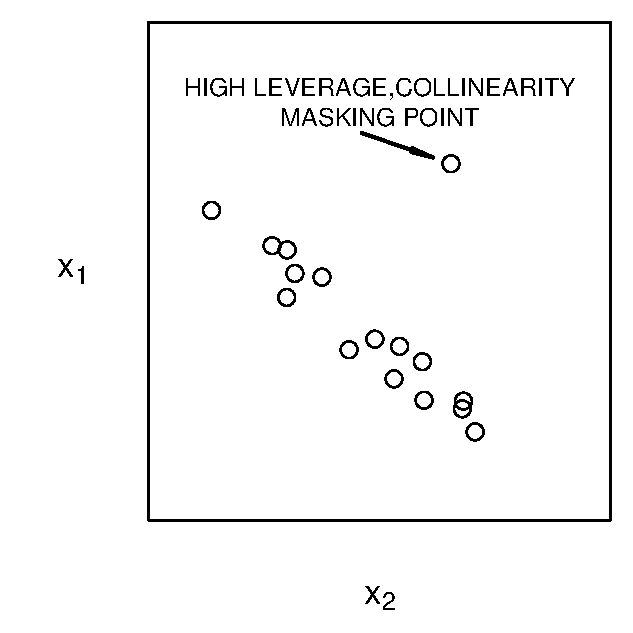
\includegraphics[width=0.45\textwidth]{Chapter5/F5CollMask.eps}
    $~~~~~~$
    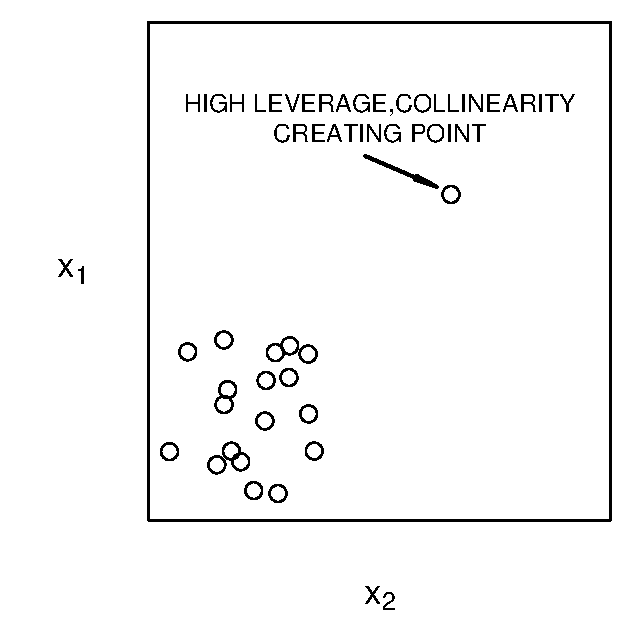
\includegraphics[width=0.45\textwidth]{Chapter5/F5CollInduce.eps}    \hfill
      \parbox[t]{2.5in}{\caption{\label{F5:CollMask} \small  With the exception of
the marked point, $x_1$ and $x_2$ are highly linearly related.}}
\hfill
        \parbox[t]{2.5in}{ \caption{\label{F5:CollInduce} \small  The highly linear relationship
between $x_1$ and $x_2$ is primarily due to the marked point.}}
\end{figure}


The examples in Figures \ref{F5:CollMask} and \ref{F5:CollInduce}
also help us to see one way in which high leverage points may affect
standard errors of regression coefficients. Recall, in Section
\ref{S5:Leverage}, we saw that high leverage points may affect the
model fitted values. In Figures \ref{F5:CollMask} and
\ref{F5:CollInduce}, we see that high leverage points affect
collinearity. Thus, from equation (\ref{E5:SEsAndVIFs}), we have
that high leverage points can also affect our standard errors of
regression coefficients.

\subsection{Suppressor Variables}\label{S5:Suppressor}\index{explanatory
variable!suppressor}

As we have seen, severe collinearity can seriously inflate standard
errors of regression coefficients. Because we rely on these standard
errors for judging the usefulness of explanatory variables, our
model selection procedures and inferences may be deficient in the
presence of severe collinearity. Despite these drawbacks, mild
collinearity in a data set should not be viewed as a deficiency of
the data set; it is simply an attribute of the available explanatory
variables.

Even if one explanatory variable is nearly a linear combination of
the others, that does not necessarily mean that the information that
it provides is redundant. To illustrate, we now consider a
\textit{suppressor variable}, an explanatory variable that increases
the importance of other explanatory variables when included in the
model.

\linejed\index{examples!suppressor variables}

\textbf{Example: Suppressor Variable.} Figure \ref{F5:Suppress}
shows a scatterplot matrix of a hypothetical data set of fifty
observations. This data set contains a response and two explanatory
variables. Table \ref{T5:Suppress} provides the corresponding matrix
of correlation coefficients. Here, we see that the two explanatory
variables are highly correlated. Now recall, for regression with one
explanatory variable, that the correlation coefficient squared is
the coefficient of determination. Thus, using Table
\ref{T5:Suppress}, for a regression of $y$ on $x_1$, the coefficient
of determination is $(0.188)^2=3.5\%$. Similarly, for a regression
of $y$ on $x_2$, the coefficient of
determination is $(-0.022)^2=0.04\%$. However, for a regression of $y$ on $%
x_1$ and $x_2$, the coefficient of determination turns out to be a
surprisingly high $80.7\%$. The interpretation is that individually, both $%
x_1$ and $x_2$ have little impact on $y$. However, when taken
jointly, the two explanatory variables have a significant effect on
$y$. Although Table \ref{T5:Suppress} shows that $x_1$ and $x_2$ are
strongly linearly related, this relationship does not mean that
$x_1$ and $x_2$ provide the same information. In fact, in this
example the two variables complement one another.

\begin{figure}[htp]
  \begin{center}
    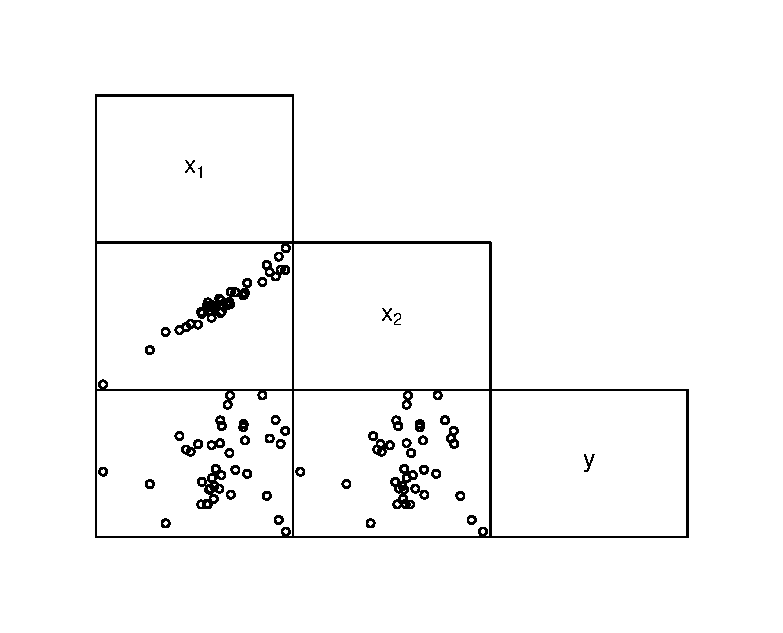
\includegraphics[width=0.6\textwidth]{Chapter5/F5Suppress.eps}
    \caption{\label{F5:Suppress} \small  Scatterplot matrix of a
response and two explanatory variable for the suppressor variable
example.}
  \end{center}
\end{figure}


\begin{table}[h]
\scalefont{0.9}

\caption{\label{T5:Suppress} Correlation Matrix for the Suppressor
Example}

\begin{tabular}{ccc}
\hline
& $x_1$ & $x_2$ \\
\multicolumn{1}{l}{$x_2$} & $0.972$ &  \\
\multicolumn{1}{l}{$y$} & $0.188$ & $-0.022$ \\ \hline
\end{tabular}
\linetjed \scalefont{1.1111}
\end{table}

\index{matrix algebra!orthogonal matrices}
\subsection{Orthogonal Variables}\label{S5:Orthogonal} Another way to understand the impact of
collinearity is to study the case when there are \emph{no}
relationships among sets of explanatory variables. Mathematically,
two matrices $\mathbf{X}_1$ and $\mathbf{X}_2$ are said to be
\emph{orthogonal} if $\mathbf{X}_1^{\prime}\mathbf{X}_2=
\mathbf{0}.$ Intuitively, because we generally work with centered
variables (with zero averages), this means that each column of
$\mathbf{X}_1$ is uncorrelated with each column of $\mathbf{X}_2$.
Although unlikely to occur with observational data in the social
sciences, when designing experimental treatments or constructing
high degree polynomials, applications of orthogonal variables are
regularly used (see for example, Hocking, 2003). For our purposes,
we will work with orthogonal variables simply to understand the
logical consequences of a total lack of collinearity.

Suppose that $\mathbf{x}_2$ is an explanatory variable that is
orthogonal to $\mathbf{X}_1$, where $\mathbf{X}_1$ is a matrix of
explanatory variables that includes the intercept. Then, it is
straightforward to check that the addition of $\mathbf{x}_2$ to the
regression equation does not change the fit for coefficients
corresponding to $\mathbf{X}_1$. That is, without $\mathbf{x}_2$,
the coefficients corresponding to $\mathbf{X}_1$ would be calculated
as $\mathbf{b}_1= \left(\mathbf{X}_1^{\prime} \mathbf{X}_1
\right)^{-1} \mathbf{X}_1^{\prime} \mathbf{y}.$ Using the orthogonal
$\mathbf{x}_2$ as part of the least squares calculation would not
change the result for $\mathbf{b}_1$ (see the recursive least
squares calculation in Section 4.7.2).

Further, the variance inflation factor for $\mathbf{x}_2$ is 1,
indicating that the standard error is unaffected by the other
explanatory variables. In the same vein, the reduction in the error
sum of squares by adding the orthogonal variable $\mathbf{x}_2$ is
due only to that variable, and not its interaction with other
variables in $\mathbf{X}_1$.

Orthogonal variables can be created for observational social science
data (as well as other collinear data) using the method of
\emph{principal components}. With this method, one uses a linear
transformation of the matrix of explanatory variables of the form,
$\mathbf{X}^{\ast}=\mathbf{X} \mathbf{P}$, so that the resulting
matrix $\mathbf{X}^{\ast}$ is composed of orthogonal columns. The
transformed regression function is $\mathrm{E~}\mathbf{y}=\mathbf{X}
\boldsymbol \beta = \mathbf{X} \mathbf{P} \mathbf{P}^{-1}
\boldsymbol \beta = \mathbf{X}^{\ast} \boldsymbol \beta^{\ast}$,
where $\boldsymbol \beta^{\ast} = \mathbf{P}^{-1} \boldsymbol \beta$
is the set of new regression coefficients. Estimation proceeds as
before, with the orthogonal set of explanatory variables. By
choosing the matrix $\mathbf{P}$ appropriately, each column of
$\mathbf{X}^{\ast}$ has an identifiable contribution. Thus, we can
readily use variable selection techniques to identify the
``principal components'' portions of $\mathbf{X}^{\ast}$ to use in
the regression equation. Principal components regression is a widely
used method in some application areas, such as psychology. It can
easily address highly collinear data in a disciplined manner. The
main drawback of this technique is that the resulting parameter
estimates are difficult to interpret.\index{principal components}


\section{Selection Criteria}


\subsection{Goodness of Fit}

How well does the model fit the data? Criteria that measure the
proximity of the fitted model and realized data are known as
\emph{goodness of fit} statistics. Specifically, we interpret the
fitted value $\hat{y}_i$ to be the best model approximation of the
$i$th observation and compare it to the actual value $y_i$. In
linear regression, we examine the difference through the residual
$e_i= y_i - \hat{y}_i$; small residuals imply a good model fit. We
have quantified this through the size of the typical error $(s)$,
include the coefficient of determination $(R^2)$ and an adjusted
version $(R_{a}^2)$.

For nonlinear models, we will need additional measures and it is
helpful to introduce these measures in this simpler linear case. One
such measure is \emph{Akaike's Information Criterion} that will be
defined in terms of likelihood fits in Section 11.9.4. For linear
regression, it reduces to
\begin{equation}\label{E5:AIC}
AIC = n \ln (s^2) + n \ln (2 \pi) +n  + 3 +k.
\end{equation}
For model comparison, the smaller the $AIC,$ the better is the fit.
Comparing models with the same number of variables ($k$) means that
selecting a model with small values of $AIC$ leads to the same
choice as selecting a model with small values of the residual
standard deviation $s$. Further, a small number of parameters means
a small value of $AIC$, other things being equal. The idea is that
this measure balances the fit ($n \ln (s^2)$) with a penalty for
complexity (the number of parameters, $k+2$). Statistical packages
often omit constants such as $n \ln (2 \pi)$ and $n+3$ when
reporting $AIC$ because they do not matter when comparing models.

Section 11.9.4 will introduce another measure, the Bayes Information
Criterion ($BIC$), that gives a smaller weight to the penalty for
complexity. A third goodness of fit measure that is used in linear
regression model is the $C_p$ statistic. To define this statistic,
assume that we have available $k$ explanatory variables
$x_1,...,x_{k}$ and run a regression to get $s_{full}^2$ as the mean
square error. Now, suppose that we are considering using only $p-1$
explanatory variables so that there are $p$ regression coefficients.
With these $p-1$ explanatory variables, we run a regression to get
the error sum of squares $(Error~SS)_p$. Thus, we are in the
position to define
\begin{equation*}
C_{p}=\frac{(Error\text{ }SS)_p}{s_{full}^2}- n + 2p.
\end{equation*}
As a selection criterion, we choose the model with a ``small''
$C_{p}$ coefficient, where small is taken to be relative to $p$. In
general, models with smaller values of $C_{p}$ are more desirable.

Like the $AIC$ and $BIC$ statistics, the $C_{p}$ statistic strikes a
balance between the model fit and complexity. That is, each
statistic summarizes the trade-off between model fit and complexity,
although with different weights. For most data sets, they recommend
the same model and so an analyst can report any or all three
statistics. However, for some applications, they lead to different
recommended models. In this case, the analyst needs to rely more
heavily on non-data driven criteria for model selection (which are
always important in any regression application).


\subsection{Model Validation}\label{S5:ModelValidation}\index{model
validation}\index{model validation!data snooping}\index{model
validation!out-of-sample}\index{model validation!model development
subsample}\index{model validation!training subsample}\index{model
validation!testing subsample}\index{model validation!validation
subsample}

Model validation is the process of confirming that our proposed
model is appropriate, especially in light of the purposes of the
investigation. Recall the iterative model formulation selection
process described in Section \ref{S5:Iterative}. An important
criticism of this iterative process is that it is guilty of
\emph{data-snooping}, that is, fitting a great number of models to a
single set of data. As we saw in Section \ref{S5:Automatic} on
data-snooping in stepwise regression, by looking at a large number
of models we may overfit the data and understate the natural
variation in our representation.

We can respond to this criticism by using a technique called
\textit{out-of-sample} \textit{validation}. The ideal situation is
to have available two sets of data, one for model development and
one for model validation. We initially develop one, or several,
models on a first data set. The models developed from the first set
of data are called our \emph{candidate} models. Then, the relative
performance of the candidate models could be measured on a second
set of data. In this way, the data used to validate the model is
unaffected by the procedures used to formulate the model.

Unfortunately, rarely will two sets of data be available to the
investigator. However, we can implement the validation process by
splitting the data set into two subsamples. We call these the
\textit{model development} and \textit{validation subsamples},
respectively. They are also known as \emph{training} and
\emph{testing} samples, respectively. To see how the process works
in the linear regression context, consider the following procedure.

\bigskip
\boxedjed

\textit{Out-of-Sample Validation Procedure}

\begin{enumerate}
\item Begin with a sample size of $n$ and divide it into two
subsamples, called the model development and validation subsamples.
Let $n_1$ and $n_2$ denote the size of each subsample. In
cross-sectional regression, do this split using a random sampling
mechanism. Use the notation $i=1,...,n_1$ to
represent observations from the model development subsample and $%
i=n_1+1,...,n_1+n_2=n$ for the observations from the validation
subsample. Figure \ref{F5:ModelValidation} illustrates this
procedure.

\item  Using the model development subsample, fit a candidate model to the data
set $i=1,...,n_1$.

\item  Using the model created in Step (ii) and the explanatory variables
from the validation subsample, ``predict'' the dependent variables
in the validation subsample, $\hat{y}_i$, where
$i=n_1+1,...,n_1+n_2$. (To get these predictions, you may need to
transform the dependent variables back to the original scale.)

\item Assess the proximity of the predictions to the held-out data.
One measure is the \textit{sum of squared prediction errors}

\begin{equation}\label{E5:SSPE}
SSPE=\sum_{i=n_1+1}^{n_1+n_2}(y_i-\hat{y}_i)^2
\end{equation}\index{symbols!$SSPE$, sum of squared prediction errors}
\index{model validation!sum of squared prediction errors, $SSPE$}


Repeat Steps (ii) through (iv) for each candidate model. Choose the
model with the smallest \textit{SSPE}.

\end{enumerate}
\end{boxedminipage}
\bigskip


\begin{figure}[htp]
  \begin{center}
    \includegraphics[width=1\textwidth]{Chapter5/F5ModelValidation.eps}
    \caption{\label{F5:ModelValidation} \small  For model validation, a
data set of size $n$ is randomly split into two subsamples.}
  \end{center}
\end{figure}


There are a number of criticisms of the \textit{SSPE}. First, it is
clear that it takes a considerable amount of time and effort to
calculate this statistic for each of several candidate models.
However, as with many statistical techniques, this is merely a
matter of having specialized statistical software available to
perform the steps described above. Second, because the statistic
itself is based on a random subset of the sample, its value will
vary from analyst to analyst. This objection could be overcome by
using the first $n_1$ observations from the sample. In most
applications this is not done in case there is a lurking
relationship in the order of the observations. Third, and perhaps
most important, is the fact that the choice of the relative subset
sizes, $n_1$ and $n_2$, is not clear. Various researchers recommend
different proportions for the allocation. Snee (1977) suggests that
data-splitting not be done unless the sample size is moderately
large, specifically, $n\geq 2(k+1)+20$. The guidelines of Picard and
Berk (1990) show that the greater the number of parameters to be
estimated, the greater the proportion of observations needed for the
model development subsample. As a rule of thumb, for data sets with
100 or fewer observations, use about 25-35\% of the sample for
out-of-sample validation. For data sets with 500 or more
observations, use 50\% of the sample for out-of-sample validation.
Hastie, Tibshirani and Friedman (2001) remark that a typical split
is 50\% for development/training, 25\% for validation and the
remaining 25\% for a third stage for further validation that they
call \textit{testing.}

Because of these criticisms, several variants of the basic out-of-sample
validation process are used by analysts. Although there is no theoretically
best procedure, it is widely agreed that model validation is an important
part of confirming the usefulness of a model.

\subsection{Cross-Validation}\label{S5:CrossV}\index{model validation!cross-validation}
\index{model validation!leave-one-out cross-validation}

Cross-validation is the technique of model validation that splits
the data into two disjoint sets. Section \ref{S5:ModelValidation}
discussed out-of-sample validation where the data was split randomly
into two subsets both containing a sizeable percentage of data.
Another popular method is \emph{leave-one-out} cross-validation,
where the validation sample consists of a single observation and the
development sample is based on the remainder of the data set.

Especially for small sample sizes, an attractive leave-one-out
cross-validation statistic is \textit{PRESS}, the \textit{Predicted
Residual Sum of Squares}. To define the statistic, consider the
following procedure where we suppose that a candidate model is
available.

\bigskip
\boxedjed

\textit{PRESS Validation Procedure}\index{symbols!$PRESS$, predicted
residual sum of squares}\index{model validation!predicted residual
sum of squares, $PRESS$}

\begin{enumerate}
\item From the full sample, omit the $i$th point and use the remaining
$n-1$ observations to compute regression coefficients.

\item Use the regression coefficients computed in step one and the explanatory
variables for the $i$th observation to compute the predicted response, $\hat{y}%
_{(i)}$. This part of the procedure is similar to the calculation of
the \textit{SSPE} statistic with $n_1=n-1$ and $n_2=1$.

\item Now, repeat (i) and (ii) for $i=1,...,n$. Summarizing, define
\begin{equation}\label{E5:PressDef}
PRESS=\sum_{i=1}^{n}(y_i-\hat{y}_{(i)})^2.
\end{equation}

\end{enumerate}

\noindent As with \textit{SSPE}, this statistic is calculated for
each of several competing models. Under this criterion, we choose
the model with the smallest \textit{PRESS}.

\end{boxedminipage}
\bigskip

Based on this definition, the statistic seems very computationally
intensive in that it requires $n$ regression fits to evaluate it. To
address this, interested readers will find that Section
\ref{S5:LOOStatistics} establishes

\begin{equation} \label{E5:StudentResid}
y_i-\hat{y}_{(i)}=\frac{e_i}{1-h_{ii}}.
\end{equation}
Here, $e_i$ and $h_{ii}$ represent the $i$th residual and leverage
from the regression fit using the complete data set. This yields


\begin{equation}\label{E5:Press}
PRESS=\sum_{i=1}^{n}\left(\frac{e_i}{1-h_{ii}}\right)^2,
\end{equation}
which is a much easier computational formula. Thus, the
\textit{PRESS} statistic is less computationally intensive than
\textit{SSPE}.

Another important advantage of this statistic, when compared to
\textit{SSPE}, is that we do not need to make an arbitrary choice as
to our relative subset sizes split. Indeed, because we are
performing an ``out-of-sample'' validation for each observation, it
can be argued that this procedure is more efficient, an especially
important consideration when the sample size is small (say, less
than 50 observations). A disadvantage is that because the model is
re-fit for each point deleted, \textit{PRESS} does not enjoy the
appearance of independence between the estimation and prediction
aspects, unlike \textit{SSPE}.



\section{Heteroscedasticity}\label{S5:Heteroscedasticity}\index{heteroscedasticity}

In most regression applications, the goal is to understand
determinants of the regression function $\mathrm{E~}y_i =
\mathbf{x}_i^{\prime} \boldsymbol \beta =\mu_i$. Our ability to
understand the mean is strongly influenced by the amount of spread
from the mean that we quantify using the variance
$\mathrm{E}\left(y_i-\mu_i\right)^2$. In some applications, such as
when I weigh myself on a scale, there is relatively little
variability; repeated measurements yield almost the same result. In
other applications, such as the time it takes me to fly to New York,
repeated measurements yield substantial variability and are fraught
with inherent uncertainty.

The amount of uncertainty can also vary on a case-by-case basis. We
denote the case of ``varying variability'' with the notation
$\sigma_i^2=\mathrm{E}\left(y_i-\mu_i\right)^2$. When the
variability varies by observation, this is known as
\emph{heteroscedasticity} for ``different scatter.''  In contrast,
the usual assumption of common variability (assumption E3/F3 in
Section 3.2) is called \textit{homoscedasticity}, meaning ``same
scatter.''\index{homoscedasticity}

Our estimation strategies depend on the extent of
heteroscedasticity. For datasets with only a mild amount of
heteroscedasticity, one can use least squares to estimate the
regression coefficients, perhaps combined with an adjustment for the
standard errors (described in Section \ref{S5:HeteroStdErrors}).
This is because least squares estimators are unbiased even in the
presence of heteroscedasticity (see Property 1 in Section 3.2).

However, with heteroscedastic dependent variables, the Gauss-Markov
theorem no longer applies and so the least squares estimators are
not guaranteed to be optimal. In cases of severe heteroscedasticity,
alternative estimators are used, the most common being those based
on transformations of the dependent variable, as will be described
in Section \ref{S5:Transformations}.\index{theorems!Gauss-Markov}

\subsection{Detecting Heteroscedasticity}

To decide a strategy for handling potential heteroscedasticity, we
must first assess, or detect, its presence.

To detect heteroscedasticity graphically, a good idea is to perform
a preliminary regression fit of the data and plot the residuals
versus the fitted values. To illustrate, Figure
\ref{F5:HeteroRegress} is a plot of a fictitious data set with one
explanatory variable where the scatter increases as the explanatory
variable increases. A least squares regression was performed -
residuals and fitted values were computed. Figure
\ref{F5:HeteroResid} is an example of a plot of residuals versus
fitted values. The preliminary regression fit removes many of the
major patterns in the data and leaves the eye free to concentrate on
other patterns that may influence the fit. We plot residuals versus
fitted values because the fitted values are an approximation of the
expected value of the response and, in many situations, the
variability grows with the expected response.

\marginparjed{To detect heteroscedasticity, plot the residuals
versus the fitted values.}

\begin{figure}[htp]
    \includegraphics[width=0.45\textwidth]{Chapter5/F5HeteroRegress.eps}
    $~~~~~~$
    \includegraphics[width=0.45\textwidth]{Chapter5/F5HeteroResid.eps}    \hfill
      \parbox[t]{2.5in}{\caption{\label{F5:HeteroRegress} \small  The shaded area
represents the data. The line is the true regression line.}} \hfill
        \parbox[t]{2.5in}{ \caption{\label{F5:HeteroResid} \small  Residuals plotted
versus the fitted values for the data in Figure
\ref{F5:HeteroRegress}.}}
\end{figure}

More formal tests of heteroscedasticity are also available in the
regression literature. To illustrate, let us consider a test due to
Breusch and Pagan (1980). Specifically, this test examines the
alternative hypothesis $H_a$: $\mathrm{Var~} y_i = \sigma^2 +
\mathbf{z}_i^{\prime} \boldsymbol \gamma $, where $\mathbf{z}_i$ is
a known vector of variables and $\boldsymbol \gamma$ is a
$p$-dimensional vector of parameters. Thus, the null hypothesis is
$H_0:~ \boldsymbol \gamma = \mathbf{0}$ is equivalent to
homoscedasticity,  $\mathrm{Var~} y_i = \sigma^2.$

\bigskip

\boxedjed

\textit{Procedure to Test for Heteroscedasticity}
\begin{enumerate}
  \item Fit a regression model and calculate the model residuals, ${e_i}$.
  \item Calculate squared standardized residuals, $e_i^{\ast 2}=e_i^2/s^2$ .
  \item  Fit a
regression model of $e_i^{\ast 2}$ on $\mathbf{z}_i$.
\item The test statistic is $LM = (Regress~SS_z)/2$, where $Regress~SS_z$ is the regression sum of squares from the
model fit in step (iii).
\item Reject the null hypothesis if $LM$ exceeds a
percentile from a chi-square distribution with $p$ degrees of
freedom. The percentile is one minus the significance level of the
test.
\end{enumerate}\index{distributions!chi-square}

\end{boxedminipage}

\bigskip

\noindent Here, we use $LM$ to denote the test statistic because
Breusch and Pagan derived it as a Lagrange multiplier statistic; see
Breusch and Pagan (1980) for more details.


\subsection{Heteroscedasticity-Consistent Standard
Errors}\label{S5:HeteroStdErrors}

For datasets with only mild heteroscedasticity, a sensible strategy
is to employ least squares estimators of the regression coefficients
and to adjust the calculation of standard errors to account for the
heteroscedasticity.

From the Section 3.2 on properties, we saw that least squares
regression coefficients could be written as $ \mathbf{b} =
\sum_{i=1}^n \mathbf{w}_i y_i $, where $\mathbf{w}_i =\left(
\mathbf{X}^{\prime}\mathbf{X}\right)^{-1} \mathbf{x}_i$. Thus, with
$\sigma_i^2 = \mathrm{Var~} y_i$, we have
\begin{equation}\label{E5:HeterVariances}
\mathrm{Var~}\mathbf{b} = \sum_{i=1}^n \mathbf{w}_i
\mathbf{w}_i^{\prime} \sigma_i^2  \\
=\left( \mathbf{X}^{\prime}\mathbf{X}\right)^{-1} \left(
\sum_{i=1}^n \sigma_i^2 \mathbf{x}_i \mathbf{x}_i^{\prime} \right)
\left( \mathbf{X}^{\prime}\mathbf{X}\right)^{-1}.
\end{equation}
This quantity is known except for $\sigma_i^2$. We can compute
residuals using the least squares regression coefficients as $e_i =
y_i - \mathbf{x}_i^{\prime} \mathbf{b}$. With these, we may define
the \emph{empirical}, or \emph{robust}, estimate of the variance
covariance matrix as
\begin{equation*}
\widehat{\mathrm{Var~}\mathbf{b}} =\left(
\mathbf{X}^{\prime}\mathbf{X}\right)^{-1} \left( \sum_{i=1}^n e_i^2
\mathbf{x}_i \mathbf{x}_i^{\prime} \right) \left(
\mathbf{X}^{\prime}\mathbf{X}\right)^{-1}.
\end{equation*}
The corresponding ``heteroscedasticity-consistent" standard errors
are
\begin{equation}\label{E5:RobustSEs}
se_r(b_j) = \sqrt{(j+1)^{st} ~diagonal~
element~of~\widehat{\mathrm{Var~}\mathbf{b}}}.
\end{equation}
The logic behind this estimator is that each squared residual,
$e_i^2$ may be a poor estimate of $\sigma_i^2$. However, our
interest is estimating a (weighted) sum of variances in equation
(\ref{E5:HeterVariances}); estimating the sum is a much easier task
than estimating any individual variance estimate.

Robust, or heteroscedasticity-consistent, standard errors are widely
available in statistical software packages. Here, you will also see
alternative definitions of residuals employed, as in Section
\ref{S5:Residuals}. If your statistical package offers options, the
robust estimator using studentized residuals is generally preferred.


\subsection{Weighted Least Squares}\label{S5:WeightedLS}\index{least
squares!weighted}

The least squares estimators are less useful for datasets with
severe heteroscedasticity. One strategy is to use a variation of
least squares estimation by \emph{weighting} observations. The idea
is that, when minimizing the sum of squared errors using
heteroscedastic data, the expected variability of some observations
is smaller than others. Intuitively, it seems reasonable that the
smaller the variability of the response, the more reliable that
response and the greater weight that it should receive in the
minimization procedure. \textit{Weighted least squares} is a
technique that accounts for this ``varying variability.''

Specifically, we use Section 3.2.3 assumptions E1, E2 and E4, with
E3 replaced by E $\varepsilon_i = 0$ and Var $\varepsilon_i =
\sigma^2 / w_i$, so that the variability is proportional to a known
weight $w_i$. For example, if unit of analysis $i$ represents a
geographical entity such as a state, you might use the number of
people in the state as a weight. Or, if $i$ represents a firm, you
might use firm assets for the weighting variable. Larger values of
$w_i$ indicate a more precise response variable through the smaller
variability. In actuarial applications, weights are used to account
for an exposure such as the amount of insurance premium, number of
employees, size of the payroll, number of insured vehicles and so
forth (further discussion is in Chapter 18).

This model can be readily converted to the ``ordinary'' least
squares problem by multiplying all regression variables by
$\sqrt{w_i}.$ That is, if we define $y_i^{\ast} = y_i \times
\sqrt{w_i}$ and $x_{ij}^{\ast} = x_{ij} \times \sqrt{w_i}$, then
from assumption E1 we have
\begin{eqnarray*}
y_i^{\ast} = y_i \times \sqrt{w_i} &=& \left( \beta_0 x_{i0}+\beta_1
x_{i1}+\ldots+\beta_k x_{ik}+\varepsilon_i \right) \sqrt{w_i}\\
&=&\beta_0 x_{i0}^{\ast} +\beta_1 x_{i1}^{\ast}+\ldots+\beta_k
x_{ik}^{\ast} + \varepsilon_i^{\ast}
\end{eqnarray*}
where $\varepsilon_i^{\ast}=\varepsilon_i \times \sqrt{w_i}$ has
homoscedastic variance $\sigma^2$. Thus, with the rescaled
variables, all inference can proceed as before.

This work has been automated in statistical packages where the user
merely specifies the weights $w_i$ and the package does the rest. In
terms of matrix algebra, this procedure can be accomplished by
defining an $n \times n$ weight matrix $\mathbf{W} = diag(w_i)$ so
that the $i$th diagonal element of $\mathbf{W}$ is $w_i$. Extending
equation (3.14) for example, the weighted least squares estimates
can be expressed as
\begin{equation}\label{E5:WLSCoefficients}
\mathbf{b}_{WLS} = \left(\mathbf{X}^{\prime} \mathbf{W}\mathbf{X}
\right)^{-1}\mathbf{X}^{\prime} \mathbf{W}\mathbf{y} .
\end{equation}
Additional discussions of weighted least squares estimation will be
presented in Section 15.1.1.


\subsection{Transformations}\label{S5:Transformations}

Another approach that handles severe heteroscedasticity, introduced
in Section 1.3, is to transform the dependent variable, typically
with a logarithmic transformation of the form $y^{\ast} =
\mathrm{ln~}y$. As we saw in Section 1.3, transformations can serve
to ``shrink'' spread out data and symmetrize a distribution. Through
a change of scale, a transformation also changes the variability,
potentially altering a heteroscedastic dataset into a homoscedastic
one. This is both a strength and limitation of the transformation
approach - a transformation simultaneously affects both the
distribution and the heteroscedasticity.

\marginparjed{The transformation of the dependent variable affects
both the skewness of the distribution and the heteroscedasticity.}

Power transformations, such as the logarithmic transform, are most
useful when the variability of the data grows with the mean. In this
case, the transform will serve to ``shrink'' the data to a scale
that appears to be homoscedastic. Conversely, because
transformations are monotonic functions, they will not help with
patterns of variability that are non-monotonic. Further, if your
data is reasonably symmetric but heteroscedastic, a transformation
will not be useful because any choice that mitigates the
heteroscedasticity will skew the distribution.

When data are non-positive, it is common to add a constant to each
observation so that all observations are positive prior to
transformation. For example, the transform $\ln (1+y)$ accommodates
the presence of zeros. One can also multiply by a constant so that
the approximate original units are retained. For example, the
transform $100\ln (1+y/100)$ may applied to percentage data where
negative percentages sometimes appear.

Our discussions of transformations have focussed on transforming
dependent variables. As noted in Section 3.5, transformations of
explanatory variables are also possible. This is because the
regression assumptions condition on explanatory variables (Section
3.2.3). Some analysts prefer to transform variables to approximate
normality, thinking of multivariate normal distributions as a
foundation for regression analysis. Others are reluctant to
transform explanatory variables because of the difficulties in
interpreting resulting models. The approach taken here is to use
transforms that can be readily interpretable, such as those
introduced in Section 3.5. Other transforms are certainly candidates
to include in a selected model but they should provide substantial
dividends in terms of fit or predictive power if they are difficult
to communicate.\index{explanatory variable!transformed}


\section{Further Reading and References}

Long and Ervin (2000) gather compelling evidence for the use of
alternative \newline heteroscedasticity-consistent estimators of
standard errors that have better finite sample performance than the
classic versions. The large sample properties of empirical
estimators have been established by Eicker (1967), Huber (1967) and
White (1980) in the linear regression case. For the linear
regression case, MacKinnon and White (1985) suggest alternatives
that provide superior small-sample properties. For small samples,
the evidence is based on (1) the biasedness of the estimators, (2)
their motivation as jackknife estimators and (3) their performance
in simulation studies.\index{heteroscedasticity}\index{matrix
algebra!eigenvalue}

Other measures of collinearity based on matrix algebra concepts
involving eigenvalues, such as condition numbers and condition
indices, are used by some analysts. See Belseley, Kuh and Welsch
(1980) for a solid treatment of collinearity and regression
diagnostics. Hocking (2003) provides additional background reading
on collinearity and principal components. See Carroll and Ruppert
(1988) for further discussions of transformations in regression.

Hastie, Tibshirani and Friedman (2001) give an advanced discussion
of model selection issues, focusing on predictive aspects of models
in the language of machine learning.

\bigskip

\textbf{Chapter References}
\begin{multicols}{2}
\scalefont{0.9}

Belseley, David A., Edwin Kuh and Roy E. Welsch (1980).
\textit{Regression Diagnostics: Identifying Influential Data and
Sources of Collinearity}. Wiley, New York.

Bendel, R. B. and Afifi, A. A. (1977). Comparison of stopping rules
in forward ``stepwise'' regression. \textit{Journal of the American
Statistical Association} 72, 46-53.

Box, George E. P. (1980). Sampling and Bayes inference in scientific
modeling and robustness (with discussion). \textit{Journal of the
Royal Statistical Society}, Series A, 143, 383-430.

Breusch, T. S. and A. R. Pagan (1980).  The Lagrange multiplier test
and its applications to model specification in econometrics.
\textit{Review of Economic Studies}, 47, 239-53.

Carroll, Raymond J. and David Ruppert (1988). \textit{Transformation
and Weighting in Regression}, Chapman-Hall.

Eicker, F. (1967), Limit theorems for regressions with unequal and
dependent errors.  \textit{Proceedings of the Fifth Berkeley
Symposium on Mathematical Statistics and Probability} 1, LeCam, L.
M. and J. Neyman, editors, University of California Press, pp,
59-82.

Hadi, A. S. (1988). Diagnosing collinearity-influential
observations. \textit{Computational Statistics and Data Analysis} 7,
143-159.

Hastie, Trevor, Robert Tibshirani and Jerome Friedman (2001).
\textit{The Elements of Statistical Learning: Data Mining, Inference
and Prediction.} Springer-Verlag, New York.

Hocking, Ronald R. (2003). \textit{Methods and Applications of
Linear Models: Regression and the Analysis of Variance}. Wiley, New
York.

Huber, P. J. (1967). The behaviour of maximum likelihood estimators
under non-standard conditions. \textit{Proceedings of the Fifth
Berkeley Symposium on Mathematical Statistics and Probability} 1,
LeCam, L. M. and Neyman, J. editors, University of California Press,
pp, 221-33.

Long, J.S. and L.H. Ervin (2000). Using heteroscedasticity
consistent standard errors in the linear regression model.
\textit{American Statistician} 54, 217-224.

MacKinnon, J.G. and H. White (1985). Some heteroskedasticity
consistent covariance matrix estimators with improved finite sample
properties. \textit{Journal of Econometrics} 29, 53-57.

Mason, R. L. and Gunst, R. F. (1985). Outlier-induced
collinearities. \textit{Technometrics} 27, 401-407.

Picard, R. R. and Berk, K. N. (1990). Data splitting. \textit{The
American Statistician} 44, 140-147.

Rencher, A. C. and Pun, F. C. (1980). Inflation of R2 in best subset
regression. \textit{Technometrics} 22, 49-53.

Snee, R. D. (1977). Validation of regression models. Methods and
examples. \textit{Technometrics} 19, 415-428.


\scalefont{1.1111}

\end{multicols}


\section{Exercises}

\scalefont{0.90}

\begin{exercises}


\item  You are doing regression with one explanatory variable and so
consider the basic linear regression model $y_i = \beta_0 +  \beta_1
x_i + \varepsilon_i$.

a.  Show that the $i$th leverage can be simplified to
\begin{equation*}
h_{ii} = \frac{1}{n} + \frac{(x_i - \overline{x})^2}{(n-1) s_x^2}.
\end{equation*}

b.  Show that  $\overline{h}= 2 / n$.

c.  Suppose that $h_{ii} = 6/n$ . How many standard deviations is
$x_i$ away (either above or below) from the mean?

\item Consider the output of a regression using one explanatory
variable on $n=3$ observations. The residuals and leverages are:
\scalefont{0.90}
\begin{tabular}{l|ccc}
\hline
$i$ & 1 & 2 & 3 \\
Residuals $e_i$ & 3.181 & -6.362 & 3.181 \\
Leverages $h_{ii}$ & 0.8333 & 0.3333 & 0.8333\\ \hline
\end{tabular}.\scalefont{1.1111}

Compute the $PRESS$ statistic.

\empexjed{UNLifeExpectancy}\index{datasets!national life
expectancies}

\item \textbf{National Life Expectancies.}\label{Ex:UNLIFE4} We
continue the analysis begun in Exercises 1.\ref{Ex:UNLIFE},
2.\ref{Ex:UNLIFE2}, 3.\ref{Ex:UNLIFE3} and 4.7. The focus of this
exercise is variable selection.

a. Begin with the data from $n=185$ countries throughout the world
that have valid (non-missing) life expectancies. Plot the life
expectancy versus the gross domestic product and private
expenditures on health. From these plots, describe why it is
desirable to use logarithmic transforms, lnGDP and lnHEALTH,
respectively. Also plot life expectancy versus lnGDP and lnHEALTH to
confirm your intuition.

b. Use a stepwise regression algorithm to help you select a model.
Do not consider the variables RESEARCHERS, SMOKING AND FEMALEBOSS as
these have many missing values. For the remaining variables, use
only the observations without any missing values. Do this twice,
with and without the categorical variable REGION.

c. Return to the full data set of $n=185$ countries and run a
regression model using FERTILITY, PUBLICEDUCATION and lnHEALTH as
explanatory variables.

c(i). Provide histograms of standardized residuals and leverages.

c(ii). Identify the standardized residual and leverage associated
with Lesotho, formerly Basutoland, a kingdom surrounded by South
Africa. Is this observation an outlier, high leverage point or both?

c(iii). Re-run the regression without Lesotho. Cite any differences
in the statistical coefficients between this model and the one in
part c(i).


\empexjed{TermLife}\index{datasets!term life insurance}

\item \textbf{Term Life Insurance.} We
continue our study of Term Life Insurance Demand from Chapters 3 and
4. Specifically, we examine the 2004 Survey of Consumer Finances
(SCF), a nationally representative sample that contains extensive
information on assets, liabilities, income, and demographic
characteristics of those sampled (potential U.S. customers). We
study a random sample of 500 families with positive incomes. From
the sample of 500, we initially consider a subsample of $n$=275
families that purchased term life insurance.

Consider a linear regression of LNINCOME, EDUCATION, NUMHH, MARSTAT,
AGE and GENDER on LNFACE.


a. Collinearity. Not all of the variables turned out to be
statistically significant. To investigate one possible explanation,
calculate variance inflation factors.

a(i). Briefly explain the idea of collinearity and a variance
inflation factor.

a(ii). What constitutes a large variance inflation factor?

a(iii). If a large variance inflation factor is detected, what
possible courses of action do we have to address this aspect of the
data?

a(iv). Supplement the variance inflation factor statistics with a
table of correlations of explanatory variables.  Based on these
statistics, is collinearity an issue with this fitted model? Why or
why not?


b. Unusual Points. Sometimes a poor model fit can be due to unusual
points.

b(i). Define the idea of leverage for an observation.

b(ii). For this fitted model, give standard rules of thumbs for
identifying points with unusual leverage. Identify any unusual
points from the attached summary statistics.

b(iii). An analyst is concerned with leverage values for this fitted
model and suggests using FACE as the dependent variable instead of
LNFACE. Describe how leverage values would change using this
alternative dependent variable.


c. Residual Analysis. We can learn how to improve model fits from
analyses of residuals.

c(i). Provide a plot of residuals versus fitted values. What do we
hope to learn from this type of plot? Does this plot display any
model inadequacies?

c(ii). Provide a $qq$ plot of residuals. What do we hope to learn
from this type of plot? Does this plot display any model
inadequacies?

c(iii). Provide a plot of residuals versus leverages. What do we
hope to learn from this type of plot? Does this plot display any
model inadequacies?


d. Stepwise Regression. Run a stepwise regression algorithm. Suppose
that this algorithm suggests a model using LNINCOME, EDUCATION,
NUMHH and GENDER as explanatory variables to predict the dependent
variable LNFACE.

d(i). What is the purpose of stepwise regression?

d(ii). Describe two important drawbacks of stepwise regression
algorithms.



\end{exercises}

\scalefont{1.1111}


\bigskip

\bigskip
\setcounter{equation}{13}
\section{Technical Supplements for Chapter 5}\label{S5:TechSupps}
\scalefont{0.9}

\subsection{Projection Matrix}\label{S5:ProjMatrix}

\textbf{Hat Matrix.} We define the hat matrix to be $\mathbf{H} =
\mathbf{X(X}^{\prime}\mathbf{X)}^{-1} \mathbf{X}^{\prime}$, so that
$\mathbf{\hat{y}} = \mathbf{X b} =\mathbf{Hy}$. From this, the
matrix $\mathbf{H}$ is said to \textit{project} the vector of
responses $ \mathbf{y}$ onto the vector of fitted values
$\mathbf{\hat{y}}$.


Because $\mathbf{H}^{\prime}=\mathbf{H}$, the hat matrix is
symmetric. Further, it is also an \textit{idempotent} matrix due to
the property that $\mathbf{HH}=\mathbf{H}$. To see this, we have
that
$\mathbf{HH}=\mathbf{(X(\mathbf{X}^{\prime}X)}^{\mathbf{-1}}\mathbf{X}^{\prime}\mathbf{)(X(\mathbf{
X}^{\prime}X)}^{\mathbf{-1}}\mathbf{X}^{\prime}\mathbf{)}=\mathbf{X(
\mathbf{X}^{\prime}X)}^{\mathbf{-1}}\mathbf{(\mathbf{X}^{\prime}X)(\mathbf{X}^{\prime}X)}^{\mathbf{-1}}
\mathbf{X}^{\prime}=\mathbf{X(\mathbf{X}
^{\prime}X)}^{\mathbf{-1}}\mathbf{X}^{\prime}=\mathbf{H}$.
Similarly, it is easy to check that $\mathbf{I-H}$ is idempotent.
Because \textbf{H} is idempotent, from some results in matrix
algebra, it is straightforward to show that
$\sum_{i=1}^{n}h_{ii}=k+1$. As discussed in Section
\ref{S5:Leverage}, we use our bounds and the average leverage,
$\bar{h}=(k+1)/n$, to help identify observations with unusually high
leverage.

\textbf{Variance of Residuals.} Using the model equation
$\mathbf{y}=\mathbf{X} \boldsymbol \beta + \boldsymbol \varepsilon$,
we can express the vector of residuals as
\begin{equation}\label{E5:Residuals}
\mathbf{e} = \mathbf{y} - \mathbf{\hat{y}} =
\mathbf{y-Hy}=\mathbf{(I-H)(X \boldsymbol \beta +\boldsymbol
\varepsilon)}=\mathbf{(I-H) \boldsymbol \varepsilon}.
\end{equation}
The last equality is due to the fact that
$\mathbf{(I-H)X}=\mathbf{X-HX}= \mathbf{X-X}=\mathbf{0}$. Using
$\text{Var~} \boldsymbol \varepsilon = \sigma ^2 \mathbf{I}$, we
have
\begin{equation*}
\text{Var }\mathbf{e}=\text{Var }\left[ \mathbf{(I-H)\boldsymbol \varepsilon}\right] =%
\mathbf{(I-H)}\text{Var }\boldsymbol \varepsilon \mathbf{(I-H)}=\sigma ^2\mathbf{(I-H)I(I-H)}%
=\sigma ^2\mathbf{(I-H)}.
\end{equation*}
The last equality comes from the fact that $\mathbf{I-H}$ is
idempotent. Thus, we have that
\begin{equation}\label{E5:VarResiduals}
\text{Var }e_i=\sigma ^2(1-h_{ii})\text{ \ and \ Cov }%
(e_i,e_j)=-\sigma ^2h_{ij}.
\end{equation}
Thus, although the true errors $\boldsymbol \varepsilon$ are
uncorrelated, there is a small negative correlation among residuals
$\mathbf e$.

\textbf{Dominance of the Error in the Residual.} Examining the $i$th
row of equation (\ref{E5:Residuals}), we have that the $i$th
residual
\begin{equation}\label{E5:ResidualsErrors}
e_i=\varepsilon_i - \sum_{j=1}^{n} h_{ij} \varepsilon_j
\end{equation}
can be expressed as a linear combination of independent errors. The
relation $ \mathbf{H}=\mathbf{HH}$ yields
\begin{equation}\label{E5:Leverages}
h_{ii}=\sum_{j=1}^{n} h_{ij}^2.
\end{equation}
Because $h_{ii}$ is, on average, $(k+1)/n$, this indicates that each
$h_{ij}$ is small relative to 1. Thus, when interpreting equation
(\ref{E5:ResidualsErrors}), we say that most of the information in
$e_i$ is due to $\varepsilon_i$.\index{leverage}

\textbf{Correlations with Residuals.} First define
$\mathbf{x}^j=(x_{1j},x_{2j},\dots,x_{nj})^{\prime}$ to be the
column representing the $j$ th variable. With this notation, we can
partition the matrix of explanatory variables as $\mathbf{X}=\left(
\mathbf{x}^{0},\mathbf{x}^{1},\dots,\mathbf{x}^{k} \right)$. Now,
examining the $j$th column of the relation $\mathbf{(I-H)X}=
\mathbf{0}$, we have $\mathbf{(I-H)x}^{j}=\mathbf{0}$. With
$\mathbf{e}=\mathbf{(I-H) \boldsymbol \varepsilon}$, this yields $
\mathbf{e}^{\prime}\mathbf{x}^{j}=\boldsymbol
\varepsilon^{\prime}\mathbf{(I-H)x} ^{j}=0,$ for $j=0,1,\ldots,k.$
This result has several implications. If the intercept is in the
model, then $\mathbf{x}^{0}=(1,1,\ldots,1)^{\prime}$ is a vector of
ones. Here, $\mathbf{e}^{\prime}\mathbf{x}^{0}=0$ means that
$\sum_{i=1}^{n} e_i=0$ or, the average residual is zero. Further,
because $\mathbf{e}^{\prime} \mathbf{x}^{j}=0$, it is easy to check
that the sample correlation between $\mathbf{e}$ and
$\mathbf{x}^{j}$ is zero. Along the same line, we also have that
$\mathbf{e}^{\prime}\mathbf{\hat{y}}=\mathbf{e}^{\prime}
\mathbf{(I-H)Xb}=\mathbf{0}$. Thus, using the same argument as
above, the sample correlation between $\mathbf{e}$ and
$\mathbf{\hat{y}}$ is zero.

\marginparjed{When a vector of ones is present, then the average
residual is zero.}

\textbf{Multiple Correlation Coefficient.} For an example of a
non-zero correlation, consider $r(\mathbf{y,\hat{y}})$, the sample
correlation
between $\mathbf{y}$ and $\mathbf{\hat{y}}$. Because $\mathbf{(I-H)x}^{0}=%
\mathbf{0}$, we have $\mathbf{x}^{0}=\mathbf{Hx}^{0}$ and thus, $\mathbf{%
\hat{y}}^{\prime}\mathbf{x}^{0}\mathbf{=y}^{\prime}\mathbf{Hx}^{0}\mathbf{%
=y^{\prime} x^{0}}$. Assuming
$\mathbf{x}^{0}=(1,1,\ldots,1)^{\prime}$, this means that
$\sum_{i=1}^{n}\hat{y}_i=$ $\sum_{i=1}^{n}y_i$, so that the average
fitted value is $\bar{y}$. Now,

\marginparjed{When a vector of ones is present, then the average
fitted value is $\bar{y}$.}

\begin{equation*}
r(\mathbf{y,\hat{y}})=\frac{\sum_{i=1}^{n}(y_i-\bar{y})(\hat{y}_i-\bar{y}%
)}{(n-1)s_{y}s_{\hat{y}}}.
\end{equation*}
Recall that $(n-1)s_{y}^2=\sum_{i=1}^{n}(y_i-\bar{y})^2=$ Total SS and $%
(n-1)s_{\hat{y}}^2=\sum_{i=1}^{n}(\hat{y}_i-\bar{y})^2=$ Regress SS.
Further, with $\mathbf{x}^{0}=(1,1,\ldots,1)^{\prime}$,
\begin{center}
\begin{eqnarray*}
\sum_{i=1}^{n}(y_i-\bar{y})(\hat{y}_i-\bar{y}) &=&(\mathbf{y}-\bar{y}%
\mathbf{x}^{0})^{\prime}(\mathbf{\hat{y}}-\bar{y}\mathbf{x}^{0})=\mathbf{y}%
^{\prime}\mathbf{\hat{y}}-\bar{y}^2\mathbf{x}^{0\prime }\mathbf{x}^{0} \\
&=&\mathbf{y}^{\prime}\mathbf{Xb}-n\bar{y}^2=\text{Regress SS.}
\end{eqnarray*}
\end{center}
This yields
\begin{equation}\label{E5:R2Correlation}
r(\mathbf{y,\hat{y}})=\frac{\text{Regress SS}}{\sqrt{\left(
\text{Total SS} \right) \left( \text{Regress SS}\right)
}}=\sqrt{\frac{\text{Regress SS}}{\text{Total SS}}}=\sqrt{R^2}.
\end{equation}
That is, the coefficient of determination can be interpreted as the
square root of the correlation between the observed and fitted
responses.

\subsection{Leave One Out Statistics}\label{S5:LOOStatistics}

\textbf{Notation.} To test the sensitivity of regression quantities,
there are a number of statistics of interest that are based on the
notion of ``leaving out,'' or omitting, an observation. To this end,
the subscript notation $(i)$ means to \textit{leave out} the $i$th
observation. For example, omitting the row of explanatory variables
$\mathbf{x}_i^{\prime}=(x_{i0},x_{i1},\dots,x_{ik})$ from
$\mathbf{X}$ yields $\mathbf{X}_{(i)}$, a
$(n-1)\times (k+1)$ matrix of explanatory variables. Similarly, $\mathbf{y}%
_{(i)}$ is a $(n-1)\times 1$ vector, based on removing the $i$th row from $%
\mathbf{y}$.

\textbf{Basic Matrix Result.} Suppose that $\mathbf{A}$ is an invertible, $%
p\times p$ matrix and $\mathbf{z}$ is a $p\times 1$ vector. The
following result from matrix algebra provides an important tool for
understanding leave one out statistics in linear regression
analysis.
\begin{equation}\label{E5:MatrixInversionResult}
\left( \mathbf{A-zz}^{\prime}\right) ^{-1}=\mathbf{A}^{-1}+\frac{\mathbf{A}%
^{-1}\mathbf{zz}^{\prime}\mathbf{A}^{-1}}{1-\mathbf{z}^{\prime}\mathbf{A}%
^{-1}\mathbf{z}}.
\end{equation}
To check this result, simply multiply $\mathbf{A-zz}^{\prime}$ by
the right hand side of equation (\ref{E5:MatrixInversionResult}) to
get $\mathbf{I}$, the identity matrix.

\textbf{Vector of Regression Coefficients.} Omitting the $i$th
observation, our new vector of regression coefficients is $
\mathbf{b}_{(i)}=\left(
\mathbf{X}_{(i)}^{\prime}\mathbf{X}_{(i)}\right)
^{-1}\mathbf{X}_{(i)}^{\prime}\mathbf{y}_{(i)}. $ An alternative
expression for $\mathbf{b}_{(i)}$ that is simpler to compute turns
out to be
\begin{equation}\label{E5:LOORegressionCoeff}
\mathbf{b}_{(i)}=\mathbf{b}-\frac{\left( \mathbf{X}^{\prime}\mathbf{X}%
\right) ^{-1}\mathbf{x}_i e_i}{1-h_{ii}}
\end{equation}
To verify equation (\ref{E5:LOORegressionCoeff}), first use equation
(\ref{E5:MatrixInversionResult}) with
$\mathbf{A}=\mathbf{X}^{\prime}\mathbf{X}$ and
$\mathbf{z}=\mathbf{x}_i$ to get
\begin{center}
\[
\left( \mathbf{X}_{(i)}^{\prime}\mathbf{X}_{(i)}\right)
^{-1}=(\mathbf{X}
^{\prime}\mathbf{X-x}_i\mathbf{x}_i^{\prime})^{-1}=
(\mathbf{X}^{\prime}\mathbf{X})^{-1}+\frac{\left(
\mathbf{X}^{\prime}\mathbf{X}\right) ^{-1}
\mathbf{x}_i\mathbf{x}_i^{\prime}\left(
\mathbf{X}^{\prime}\mathbf{X} \right) ^{-1}}{1-h_{ii}},
\]
\end{center}
where, from equation (\ref{E5:Leverage}), we have
$h_{ii}=\mathbf{x}_i^{\prime}
\mathbf{(X}^{\prime}\mathbf{X)}^{-1}\mathbf{x}_i$. Multiplying each
side by
$\mathbf{X}_{(i)}^{\prime}\mathbf{y}_{(i)}=\mathbf{X}^{\prime}\mathbf{y}
-\mathbf{x}_i y_i$ yields

\begin{center}
\begin{eqnarray*}
\mathbf{b}_{(i)} &=&\left(
\mathbf{X}_{(i)}^{\prime}\mathbf{X}_{(i)}\right)
^{-1}\mathbf{X}_{(i)}^{\prime}\mathbf{y}_{(i)}=\left( (\mathbf{X}^{\prime}%
\mathbf{X})^{-1}+\frac{\left( \mathbf{X}^{\prime}\mathbf{X}\right) ^{-1}%
\mathbf{x}_i\mathbf{x}_i^{\prime}\left( \mathbf{X}^{\prime}\mathbf{X}%
\right) ^{-1}}{1-h_{ii}}\right) \left( \mathbf{X}^{\prime}\mathbf{y}-%
\mathbf{x}_iy_i\right)  \\
&=&\mathbf{b}-\left( \mathbf{X}^{\prime}\mathbf{X}\right) ^{-1}\mathbf{x}%
_iy_i+\frac{\left( \mathbf{X}^{\prime}\mathbf{X}\right) ^{-1}\mathbf{x}%
_i\mathbf{x}_i^{\prime}\mathbf{b}-\left( \mathbf{X}^{\prime}\mathbf{X}%
\right) ^{-1}\mathbf{x}_i\mathbf{x}_i^{\prime}\left(
\mathbf{X}^{\prime}\mathbf{X}\right) ^{-1}\mathbf{x}_iy_i}{1-h_{ii}} \\
&=&\mathbf{b}-\frac{\left( 1-h_{ii}\right) \left( \mathbf{X}^{\prime}%
\mathbf{X}\right) ^{-1}\mathbf{x}_iy_i-\left( \mathbf{X}^{\prime}%
\mathbf{X}\right) ^{-1}\mathbf{x}_i\mathbf{x}_i^{\prime}\mathbf{b}%
-\left( \mathbf{X}^{\prime}\mathbf{X}\right) ^{-1}\mathbf{x}_ih_{ii}y_i%
}{1-h_{ii}} \\
&=&\mathbf{b}-\frac{\left( \mathbf{X}^{\prime}\mathbf{X}\right) ^{-1}%
\mathbf{x}_iy_i-\left( \mathbf{X}^{\prime}\mathbf{X}\right) ^{-1}%
\mathbf{x}_i\mathbf{x}_i^{\prime}\mathbf{b}}{1-h_{ii}}=\mathbf{b}-\frac{%
\left( \mathbf{X}^{\prime}\mathbf{X}\right) ^{-1}\mathbf{x}_i e_i}{%
1-h_{ii}}.\text{ }
\end{eqnarray*}%
\qquad
\end{center}

\noindent This establishes equation (\ref{E5:LOORegressionCoeff}).

\textbf{Cook's Distance.} To measure the effect, or
\textit{influence}, of omitting the \textit{i}th observation, Cook
examined the difference between fitted values with and without the
observation. We define Cook's Distance to be
\begin{center}
\[
D_i=\frac{\left( \mathbf{\hat{y}-\hat{y}}_{(i)}\right)
^{\prime}\left( \mathbf{\hat{y}-\hat{y}}_{(i)}\right) }{(k+1)s^2}
\]
\end{center}
where $\mathbf{\hat{y}}_{(i)}=\mathbf{Xb}_{(i)}$ is the vector of
fitted values calculated omitting the $i$th point. Using equation
(\ref{E5:LOORegressionCoeff}) and $\mathbf{\hat{y}}=\mathbf{Xb}$, an
alternative expression for Cook's Distance is
\begin{center}
\begin{eqnarray*}
D_i &=&\frac{\left( \mathbf{b-b}_{(i)}\right) ^{\prime}\left( \mathbf{X}%
^{\prime}\mathbf{X}\right) \left( \mathbf{b-b}_{(i)}\right) }{(k+1)s^2} \\
&=&\frac{e_i^2}{(1-h_{ii})^2}\frac{\mathbf{x}_i^{\prime}\left(
\mathbf{X}^{\prime}\mathbf{X}\right) ^{-1} \left(
\mathbf{X}^{\prime}\mathbf{X}\right) \left(
\mathbf{X}^{\prime}\mathbf{X}\right) ^{-1}\mathbf{x}_i}{(k+1)s^2} \\
&=&\frac{e_i^2}{(1-h_{ii})^2}\frac{h_{ii}}{(k+1)s^2}=\left(
\frac{e_i^2}{s\sqrt{1-h_{ii}}}\right) ^2\frac{h_{ii}}{%
(k+1)(1-h_{ii})}.
\end{eqnarray*}
\end{center}
This result is not only useful computationally, it also serves to
decompose the statistic into the part due to the standardized
residual, $\left( e_i/\left( s\left( 1-h_{ii}\right) ^{1/2}\right)
\right) ^2$, and due to the leverage, $h_{ii}/\left( \left(
k+1\right) \left( 1-h_{ii}\right) \right) $.\index{leverage}


\textbf{Leave One Out Residual.} The leave one out residual is defined by $%
e_{(i)}=y_i-\mathbf{x}_i^{\prime}\mathbf{b}_{(i)}$. It is used in
computing the \textit{PRESS} statistic, described in Section
\ref{S5:CrossV}. A simple computational expression is
$e_{(i)}=e_i/(1-h_{ii})$. To verify this, use equation
(\ref{E5:LOORegressionCoeff}) to get
\begin{center}
\begin{eqnarray*}
e_{(i)} &=&y_i-\mathbf{x}_i^{\prime}\mathbf{b}_{(i)}=y_i-%
\mathbf{x}_i^{\prime}\left( \mathbf{b}-\frac{\left( \mathbf{X}^{\prime}%
\mathbf{X}\right) ^{-1}\mathbf{x}_ie_i}{1-h_{ii}}\right)  \\
&=&e_i+\frac{\mathbf{x}_i\left( \mathbf{X}^{\prime}\mathbf{X}%
\right) ^{-1}\mathbf{x}_ie_i}{1-h_{ii}}=e_i+\frac{h_{ii}
e_i}{1-h_{ii}}=\frac{e_i}{1-h_{ii}}.
\end{eqnarray*}
\end{center}

\textbf{Leave One Out Variance Estimate.} The leave one out estimate
of the variance is defined by
$s_{(i)}^2=((n-1)-(k+1))^{-1}\sum_{j\neq i}\left(
y_j-\mathbf{x}_j^{\prime}\mathbf{b}_{(i)}\right) ^2$. It is used in
the definition of the \textit{studentized residual}, defined in
Section \ref{S5:Residuals}. A simple computational expression is
given by
\begin{equation}\label{E5:LOOVarianceEstimate}
s_{(i)}^2=\frac{(n-(k+1))s^2-\frac{e_i^2}{1-h_{ii}}}{%
(n-1)-(k+1)}.
\end{equation}
To see this, first note that from equation (\ref{E5:Residuals}), we have $\mathbf{He%
}=\mathbf{H(I-H)\boldsymbol \varepsilon}=\mathbf{0}$, because
$\mathbf{H}=\mathbf{HH}$. In
particular, from the $i$th row of $\mathbf{He}=\mathbf{0}$, we have $%
\sum_{j=1}^{n}h_{ij}e_j=0$. Now, using equations
(\ref{E5:Leverages}) and (\ref{E5:LOORegressionCoeff}), we have

\begin{center}
\begin{eqnarray*}
\sum_{j\neq i}\left(
y_j-\mathbf{x}_j^{\prime}\mathbf{b}_{(i)}\right)
^2 &=&\sum_{j=1}^{n}\left( y_j-\mathbf{x}_j^{\prime}\mathbf{b}%
_{(i)}\right) ^2-\left( y_i-\mathbf{x}_i^{\prime}\mathbf{b}%
_{(i)}\right) ^2 \\
&=&\sum_{j=1}^{n}\left( y_j-\mathbf{x}_j^{\prime}\mathbf{b}+\frac{%
\mathbf{x}_j^{\prime}\mathbf{(X}^{\prime}\mathbf{X)}^{-1}\mathbf{x}_i%
e_i}{1-h_{ii}}\right) -e_{(i)}^2 \\
&=&\sum_{j=1}^{n}(e_j+\frac{h_{ij}e_i}{1-h_{ii}})^2-\frac{%
e_i^2}{(1-h_{ii})^2} \\
&=&\sum_{j=1}^{n}e_j^2+0+\frac{e_i^2}{(1-h_{ii})^2}%
h_{ii}-\frac{e_i^2}{(1-h_{ii})^2} \\
&=&\sum_{j=1}^{n}e_j^2-\frac{e_i^2}{1-h_{ii}}%
=(n-(k+1))s^2-\frac{e_i^2}{1-h_{ii}}.
\end{eqnarray*}%
\qquad
\end{center}

This establishes equation (\ref{E5:LOOVarianceEstimate}).

\subsection{Omitting Variables}\label{S5:OmittingVariables}

\textbf{Notation.} To measure the effect on regression quantities,
there are a number of statistics of interest that are based on the
notion of omitting an explanatory variable. To this end, the
superscript notation $(j)$ means to omit the $j$th variable, where
$j=0,1,...,k$. First, recall that
$\mathbf{x}^{j}=(x_{1j},x_{2j},\ldots,x_{nj})^{\prime}$ is the
column representing the $j$ th variable. Further, define
$\mathbf{X}^{(j)}$ to be the $n\times k$ matrix of explanatory
variables defined by removing $\mathbf{x}^{j}$ from $\mathbf{X}$.
For example, taking $j=k$, we often partition $\mathbf{X}$ as
$\mathbf{X} =\left( \mathbf{X}^{(k)}: \mathbf{x}^k \right) $.
Employing the results of Section 4.7.2, we will use
$\mathbf{X}^{(k)} = \mathbf{X}_1$ and $\mathbf{x}^k =
\mathbf{X}_2.$


\textbf{Variance Inflation Factor}. We first would like to establish
the relationship between the definition of the standard error of
$b_j$ given by
\begin{equation*}
se(b_j)=s\sqrt{(j+1)\text{th \textit{diagonal element} of }\mathbf{(X}%
^{\prime}\mathbf{X)}^{-1}}
\end{equation*}
and the relationship involving the variance inflation factor,
\begin{equation*}
se(b_j)=s\frac{\sqrt{VIF_j}}{s_{x_j}\sqrt{n-1}}.
\end{equation*}
By symmetry of the independent variables, we only need consider only
the case where $j=k$. Thus, we would like to establish
\begin{equation}\label{E5:VIFXPX}
(k+1)\text{st diagonal element of }(\mathbf{X}^{\prime}\mathbf{X}%
)^{-1}=VIF_{k}/((n-1)s_{x_{k}}^2).
\end{equation}
First consider the reparameterized model in equation (4.22). From
equation (4.23), we can express the regression coefficient estimate
$b_{k} =
(\mathbf{e}_1^{\prime}\mathbf{y})/(\mathbf{e}_1^{\prime}\mathbf{e}_1)$.
From equation (4.23), we have that Var $b_{k} = \sigma ^2(
\mathbf{E}_2^{\prime}\mathbf{E}_2)^{-1}$ and thus
\begin{equation}\label{E5:StdErrorReparam}
se(b_{k})=s(\mathbf{E}_2^{\prime}\mathbf{E}_2)^{-1/2}.
\end{equation}
Thus, the $(\mathbf{E}_2^{\prime}\mathbf{E}_2)^{-1}$ is $(k+1)$st
diagonal element of $ \left(
\begin{bmatrix} \mathbf{X}_1^{\prime} \\ \mathbf{E}_2^{\prime}
\end{bmatrix}
\begin{bmatrix}
\mathbf{X}_1 & \mathbf{E}_2
\end{bmatrix} \right)^{-1}$
and is also the $(k+1)$st diagonal element of $(\mathbf{X}^{\prime}
\mathbf{X})^{-1}$. Alternatively, this can be verified directly
using the partitioned matrix inverse in equation (4.19).

Now, suppose that we run a regression using
$\mathbf{x}^{k}=\mathbf{X}_2$ as the response vector and
$\mathbf{X}^{(k)}=\mathbf{X}_1$ as the matrix of explanatory
variables. As noted above equation (4.22), $\mathbf{E}_2$ represents
the ``residuals'' from this regression and thus
$\mathbf{E}_2^{\prime}\mathbf{E}_2$ represents the error sum of
squares. For this regression, the total sum of squares is
$\sum_{i=1}^{n}(x_{ik}-\bar{x}_{k})^2 = (n-1)s_{x_{k}}^2$ and the
coefficient of determination is $R_{k}^2$. Thus,
\begin{equation*}
\mathbf{E}_2^{\prime}\mathbf{E}_2 = \text{``Error SS''}=\text{%
``Total SS'' }(1-R_{k}^2)=(n-1)s_{x_{k}}^2/VIF_{k}.
\end{equation*}
This establishes equation (\ref{E5:VIFXPX}).


\textbf{Establishing }$\mathbf{t}^{\mathbf{2}}\mathbf{=F}$. For
testing the null hypothesis H$_0$: $\beta_{k}=0$, the material in
Section 3.4.1 provides a description of a test based on the
\textit{t-}statistic, $t(b_{k})=b_{k}/se(b_{k})$. An alternative
test procedure, described in Sections 4.2.2, uses the test statistic
\begin{equation*}
F-\text{ratio} = \frac{(Error~SS)_{reduced}-(Error~SS)_{full}} {p
\times (Error~MS)_{full}} = \frac{\left(
\mathbf{E}_2^{\prime}\mathbf{y}\right) ^2}{s^2\mathbf{E}_2^{\prime}
\mathbf{E}_2}
\end{equation*}
from equation (4.26). Alternatively, from equations (4.23) and
(\ref{E5:StdErrorReparam}), we have
\begin{equation}\label{E5:tStat}
t(b_{k})=\frac{b_{k}}{se(b_{k})}=\frac{\left( \mathbf{E}_2^{\prime}
\mathbf{y}\right) /\left( \mathbf{E}_2^{\prime}\mathbf{E}_2\right)}
{s/\sqrt{\mathbf{E}_2^{\prime}\mathbf{E}_2}}= \frac{\left(
\mathbf{E}_2^{\prime}\mathbf{y}\right) }{s\sqrt{
\mathbf{E}_2^{\prime}\mathbf{E}_2}}.
\end{equation}

\noindent Thus, $t(b_{k})^2=F-$ratio.

\index{correlation coefficients!partial}

\textbf{Partial Correlation Coefficients.} From the full regression
model $ \mathbf{y}=\mathbf{X}^{(k)}\boldsymbol
\beta^{(k)}+\mathbf{x}_{k}\beta_{k}+\boldsymbol \varepsilon$,
consider two separate regressions. A regression using
$\mathbf{x}^{k}$ as the response vector and $\mathbf{X}^{(k)}$ as
the matrix of explanatory variables yields the residuals
$\mathbf{E}_2$. Similarly, a regression $\mathbf{y}$ as the response
vector and $\mathbf{X}^{(k)}$ as the matrix of explanatory variables
yields the residuals
\begin{equation*}
\mathbf{E}_1 = \mathbf{y} - \mathbf{X}^{(k)} \left(
\mathbf{X}^{(k)\prime} \mathbf{X}^{(k)}\right)^{-1} \mathbf{X}^{(k)}
\mathbf{y.}
\end{equation*}
If $x^{0}=(1,1,\ldots,1)^{\prime}$, then the average of $
\mathbf{E}_1$ and $\mathbf{E}_2$ is zero. In this case, the sample
correlation between $\mathbf{E}_1$ and $\mathbf{E}_2$ is
\begin{equation*}
r(\mathbf{E}_1,\mathbf{E}_2) = \frac{\sum_{i=1}^{n} E_{1i}
E_{2i}}{\sqrt{\left( \sum_{i=1}^{n} E_{i1}^2\right) \left(
\sum_{i=1}^{n} E_{i2}^2\right) }} = \frac{\mathbf{E}_1^{\prime}
\mathbf{E}_2}{\sqrt{\left( \mathbf{E}_1^{\prime}\mathbf{E}_1\right)
\left( \mathbf{E}_2^{\prime}\mathbf{E}_2 \right) }}.
\end{equation*}
Because $\mathbf{E}_2$ is a vector of residuals using $\mathbf{X}
^{(k)}$ as the matrix of explanatory variables, we have that
$\mathbf{E}_2^{\prime} \mathbf{X}^{(k)} = 0$. Thus, for the
numerator, we have
\newline $\mathbf{E}_2^{\prime}\mathbf{E}_1 =
\mathbf{E}_2^{\prime}\left( \mathbf{y}-\mathbf{X}^{(k)}\left(
\mathbf{X}^{(k)\prime }\mathbf{X}^{(k)}\right)
^{-1}\mathbf{X}^{(k)}\mathbf{y}\right)
=\mathbf{E}_2^{\prime}\mathbf{y.}$ From equations (4.24) and (4.25),
we have that
\begin{equation*}
(n-(k+1))s^2 = (Error~SS)_{full} = \mathbf{E}_1^{\prime}
\mathbf{E}_1 - \left( \mathbf{E}_1^{\prime}\mathbf{y}\right) ^2 /
\left( \mathbf{E}_2^{\prime}\mathbf{E}_2\right) =
\mathbf{E}_1^{\prime}\mathbf{E}_1 - \left( \mathbf{E}
_1^{\prime}\mathbf{E}_2\right) ^2/\left(
\mathbf{E}_2^{\prime}\mathbf{E}_2\right).
\end{equation*}
Thus, from equation (\ref{E5:tStat})
\begin{center}
\begin{eqnarray*}
\frac{t(b_{k})}{\sqrt{t(b_{k})^2+n-(k+1)}} &=&\frac{\mathbf{E}
_2^{\prime} \mathbf{y} / \left(
s\sqrt{\mathbf{E}_2^{\prime}\mathbf{E}_2}\right) }
{\sqrt{\frac{\left( \mathbf{E}_2^{\prime} \mathbf{y}\right) ^2}
{s^2\mathbf{E}_2^{\prime}\mathbf{E}_2}+n-(k+1)}} \\
&=&\frac{\mathbf{E}_2^{\prime}\mathbf{y}}{\sqrt{\left(
\mathbf{E}_2^{\prime}\mathbf{y}\right) ^2+\mathbf{E}_2^{\prime}
\mathbf{E}_2 s^2\left( n-(k+1)\right) }} \\
&=&\frac{\mathbf{E}_2^{\prime}\mathbf{E}_1} {\sqrt{\left(
\mathbf{E}_2^{\prime}\mathbf{E}_1\right)^2 +
\mathbf{E}_2^{\prime}\mathbf{E}_2\left( \mathbf{E}_1^{\prime}
\mathbf{E}_1 - \frac{\left( \mathbf{E}_2^{\prime}\mathbf{E}_1\right)
^2}{\mathbf{E}_2^{\prime}\mathbf{E}_2}
\right) }} \\
&=&\frac{\mathbf{E}_1^{\prime}\mathbf{E}_2}{\sqrt{(\mathbf{E}_1^{\prime}\mathbf{E}_1)
(\mathbf{E}_2^{\prime} \mathbf{E}_2)}} =
r(\mathbf{E}_1,\mathbf{E}_2) .
\end{eqnarray*}
\end{center}
This establishes the relationship between the partial correlation
coefficient and the \textit{t-}ratio statistic.

\scalefont{1.1111}

\setcounter{chapter}{5}

\chapter{Interpreting Regression Results}

{\small \textit{Chapter Preview}. A regression analyst collects
data, selects a model and then reports on the findings of the study,
in that order. This chapter considers these three topics in
\emph{reverse} order, emphasizing how each stage of the study is
influenced by preceding steps. An application, determining a firm's
characteristics that influence its effectiveness in managing risk,
illustrates the regression modeling process from start to finish.}

\bigskip

\bigskip


Studying a problem using a regression modeling process involves a
substantial commitment of time and energy. One must first embrace
the concept of \emph{statistical thinking}, a willingness to use
data actively as part of a decision making process. Second, one must
appreciate the usefulness of a model that is used to approximate a
real situation. Having made this substantial commitment, there is a
natural tendency to ``oversell'' the results of statistical methods
such as regression analysis. By overselling any set of ideas,
consumers eventually become disappointed when the results do not
live up to their expectations. This chapter begins in Section 6.1 by
summarizing what we can reasonably expect to learn from regression
modeling.

\marginparjed{``All models are wrong, but some are useful.'' (Box,
1979)}

Models are designed to be much simpler than relationships among
entities that exist in the real world. A model is merely an
approximation of reality. As stated by George Box (1979), ``All
models are wrong, but some are useful.'' Developing the model, the
subject of Chapter 5, is part of the art of statistics. Although the
principles of variable selection are widely accepted, the
application of these principles can vary considerably among
analysts. The resulting product has certain aesthetic values and is
by no means predetermined. Statistics can be thought of as the art
of reasoning with data. Section 6.2 will underscore the importance
of variable selection.

Model formulation and data collection form the first stage of the
modeling process. Students of statistics are usually surprised at
the difficulty of relating ideas about relationships to available
data. These difficulties include a lack of readily available data
and the need to use certain data as proxies for ideal information
that is not available numerically. Section 6.3 will describe several
types of difficulties that can arise when collecting data. Section
6.4 will describe some models to alleviate these difficulties.

\section{What the Modeling Process Tells Us}

Model inference is the final stage of the modeling process. By
studying the behavior of models, we hope to learn something about
the real world. Models serve to impose an order on reality and
provide a basis for understanding reality through the nature of the
imposed order. Further, statistical models are based on reasoning
with the available data from a sample. Thus, models serve as an
important guide for predicting the behavior of observations outside
the available sample.

\subsection{Interpreting Individual Effects}

When interpreting results from multiple regression, the main goal is
often to convey the importance of individual variables, or effects,
on an outcome of interest. The interpretation depends on whether or
not the effects are substantively significant, statistically
significant and causal.

\index{significance!substantive}

\noindent \textbf{Substantive Significance}. Readers of a regression
study first want to understand the direction and magnitude of
individual effects. Do females have more or less claims than males
in a study of insurance claims? If less, by how much? You can give
answers to these questions through a table of regression
coefficients. Moreover, to give a sense of the reliability of the
estimates, you may also wish to include the standard error or a
confidence interval, as introduced in Section 3.4.2.

Recall that regression coefficients are estimates of partial
derivatives of the regression function
\begin{equation*}
\mathrm{E~}y = \beta_0 + \beta_1 x_1 +...+\beta _k x_k.
\end{equation*}
When interpreting coefficients for continuous explanatory variables,
it is helpful to do so in terms of meaningful changes of each $x$.
For example, if population is an explanatory variable, we may talk
about the expected change in $y$ per 1,000 or one million change in
population. Moreover, when interpreting regression coefficients,
comment on their ``substantive'' significance. For example, suppose
that we find a difference in claims between males and females but
the estimated difference is only 1\% of expected claims. This
difference may well be statistically significant but not
economically meaningful. Substantive significance refers to
importance in the field of inquiry; in actuarial science, this is
typically financial or economic significance but could also be
non-monetary, such as effects on future life expectancy.

\marginparjed{Substantive significance refers to importance in the
field of inquiry.}

\index{significance!statistical}

\noindent \textbf{Statistical Significance}. Are the effects due to
chance? The hypothesis testing machinery introduced in Section 3.4.1
provides a formal mechanism for answering this question. Tests of
hypotheses are useful in that they provide a formal, agreed-upon
standard, for deciding whether or not a variable provides an
important contribution to an expected response. When interpreting
results, typically researchers cite a $t$-ratio or a $p$-value to
demonstrate statistical significance.

In some situations, it is of interest to comment on variables that
are \emph{not} statistically significant. Effects that are not
statistically significant have standard errors that are large
relative to the regression coefficients. In Section 5.5.2, we
expressed this standard error as
\begin{equation}\label{E6:StdErrorBeta}
se(b_{j})=s\frac{\sqrt{VIF_{j}}}{s_{x_{j}}\sqrt{n-1}}.
\end{equation}
One possible explanation for a lack of statistical significance is a
large variation in the disturbance term. By expressing the standard
error in this form, we see that the larger the natural variation, as
measured by $s$, the more difficult it is to reject the null
hypothesis of no effect ($H_0$), other things being equal.

A second possible explanation for the lack of statistical
significant is the high collinearity, as measured by $VIF_j$. A
variable may be be confounded with other variables such that, from
the data being analyzed, it is impossible to distinguish the effects
of one variable from another.

A third possible explanation is the sample size. Suppose that a
mechanism similar to draws from a stable population is used to
observe the explanatory variables. Then, the standard deviation of
$x_j,s_{x_j},$ should be stable as the number of draws increases.
Similarly, so should $R_j^2$ and $s^2$. Then, the standard error
$se(b_j)$ should decrease as the sample size, $n$, increases.
Conversely, a smaller sample size means a larger standard error,
other things being equal. This means that we may not be able to
detect the importance of variables in small or moderate size
samples.

Thus, in an ideal world, if you do not detect statistical
significance where it was hypothesized (and fully expected), you
could: (i) get a more precise measure of $y$, thus reducing its
natural variability, (ii) re-design the sample collection scheme so
that the relevant explanatory variables are less redundant and (iii)
collect more data. Typically, these options are not available with
observational data but it can nonetheless be helpful to point out
the next steps in a research program.


\marginparjed{Large samples provide an opportunity to detect the
importance of variables that might go unnoticed in small samples.}

Analysts occasionally observe statistically significant
relationships that were not anticipated - these could be due to a
large sample size. Above we noted that a small sample may not
provide enough information to detect meaningful relationships. The
flip side of this argument is that, for large samples, we have an
opportunity for detecting the importance of variables that might go
unnoticed in small or even moderate size samples. Unfortunately, it
also means that variables with small parameter coefficients, that
contribute little to understanding the variation in the response,
can be judged to be significant using our decision-making
procedures. This serves to highlight the difference between
substantive and statistical significance - particularly for large
samples, investigators encounter variables that are
\textit{statistically significant but practically unimportant}. In
these cases, it can be prudent for the investigator to omit
variables from the model specification when their presence is not in
accord with accepted theory, even if they are judged statistically
significant.

\marginparjed{Variables can be statistically significant but
practically unimportant.}

\index{significance!causal effect}

\noindent \textbf{Causal Effects}. If we change $x$, would $y$
change? As students of basic sciences, we learned principles
involving actions and reactions. Adding mass to a ball in motion
increases the force of its impact into a wall. However, in the
social sciences, relationships are probabilistic, not deterministic,
and hence more subtle. For example, as age ($x$) increases, the
one-year probability of death ($y$) increases for most human
mortality curves. Understanding causality, even probabilistic, is
the root of all science and provides the basis for informed
decision-making.

It is important to acknowledge that causal processes generally
cannot be demonstrated exclusively from the data; the data can only
present relevant empirical evidence serving as a link in a chain of
reasoning about causal mechanisms. For causality, there are three
necessary conditions: (i) statistical association between variables,
(ii) appropriate time order and (iii) the elimination of alternative
hypotheses or establishment of a formal causal mechanism.

As an example, recall the Section 1.1 Galton study, relating adult
children's height ($y$) to an index of parents' height ($x$). For
this study, it was clear that there is a strong statistical
association between $x$ and $y$. The demographics also make it clear
that the parents measurements ($x$) precedes the children
measurements ($y$). What is uncertain is the causal mechanism. For
example, in Section 1.5, we cited the possibility that an omitted
variable, family diet, could be influencing both $x$ and $y$.
Evidence and theories from human biology and genetics are needed to
establish a formal causal mechanism.

\linejed\index{examples!race, redlining and automobile insurance
prices}\index{actuarial \& financial terms and concepts!redlining}

\textbf{Example: Race, Redlining and Automobile Insurance Prices.}
In an article with this title, Harrington and Niehaus (1998)
investigated whether insurance companies engaged in (racial)
discriminatory behavior, often known as \emph{redlining}. Racial
discrimination is illegal and insurance companies may not use race
in determining prices. The term redlining refers to the practice of
drawing red lines on a map to indicate areas that insurers will not
serve, areas typically containing a high proportion of minorities.

To investigate whether or not there exists racial discrimination in
insurance pricing, Harrington and Niehaus gathered private passenger
premiums and claims data from the Missouri Department of Insurance
for the period 1988-1992. Although insurance companies do not keep
race/ethnicity information in their premiums and claims data, such
information is available at the zip code level from the US Census
Bureau. By aggregating premiums and claims up to the zip code level,
Harrington and Niehaus were able to assess whether areas with a
higher percentage of blacks paid more for insurance (PCTBLACK).

A widely used pricing measure is the loss ratio, defined to be the
ratio of claims to premiums. This measures insurers' profitably; if
racial discrimination exists in pricing, one would expect to see a
low loss ratio in areas with a high proportion of minorities.
Harrington and Niehaus used this as the dependent variable, after
taking logarithms to address the skewness in the loss ratio
distribution.

Harrington and Niehaus (1998) studied 270 zip codes surrounding six
major cities in Missouri where there were large concentrations of
minorities. Table \ref{T6:LossRatio} reports findings from
comprehensive coverage although the authors also investigated
collision and liability coverage. In addition to the primary
variable of interest, PCTBLACK, a few control variables relating to
age distribution (PCT1824 and PCT55P), marital status (MARRIED),
population (ln TOTPOP) and income (PCTUNEMP) were introduced. Policy
size was measured indirectly through an average car value (ln
AVCARV).

Table \ref{T6:LossRatio} reports that only policy size and
population are statistically significant determinants of loss
ratios. In fact, the coefficient associated with PCTBLACK has a
positive sign, indicating that premiums are lower in areas with high
concentrations of minorities (although, not significant). In an
efficient insurance market, we would expect prices to be closely
aligned with claims and that few broad patterns exist.


\begin{table}[h]
\caption{\label{T6:LossRatio} Loss Ratio Regression Results }
\begin{tabular}{ll|rr}
   \hline
  & & Regression &   $t-$ \\
   Variable  & Description  & Coefficient &  statistic \\   \hline
Intercept & & 1.98 & 2.73 \\
PCTBLACK & Proportion of population black & 0.11 & 0.63 \\
ln TOTPOP & Logarithmic total population
& -0.10 & -4.43 \\
PCT1824 & Percent of population between 18 and 24 & -0.23 & -0.50 \\
PCT55UP & Percent of population 55 or older & -0.47 & -1.76 \\
MARRIED & Percent of population married & -0.32 & -0.90 \\
PCTUNEMP  & Percent of population unemployed& 0.11 & 0.10 \\
ln AVCARV & Logarithmic average car value insured & -0.87 & -3.26 \\
  \multicolumn{2}{l}{$R_a^2$} &  \multicolumn{2}{c}{~~~~~~~~~0.11} \\
 \hline
     \multicolumn{4}{c}{\textit{Source}: Harrington and Niehaus (1998)} \\
\end{tabular}
 \linetjed
\end{table}



Certainly, the findings of Harrington and Niehaus (1998) are
inconsistent with the hypothesis of racial discrimination in
pricing. Establishing a lack of statistical significance is
typically more difficult than establishing significance. In the
paper by Harrington and Niehaus (1998), there are many alternative
model specifications that assess the robustness of their findings to
different variable selection procedures and different data subsets.
Table \ref{T6:LossRatio} reports coefficient estimators and standard
errors calculate using weighted least squares, with population size
as weights. The authors also ran (ordinary) least squares, with
robust standard errors, achieving similar results.


\subsection{Other Interpretations}

When taken collectively, linear combinations of the regression
coefficients can be interpreted as the regression function
\begin{equation*}
\mathrm{E~}y = \beta_0 + \beta_1 x_1 +...+\beta _k x_k.
\end{equation*}
When reporting regression results, readers want to know how well the
model fits the data. Section 5.6.1 summarized several goodness of
fit statistics that are routinely reported in regression
investigations.

\noindent \textbf{Regression Function and Pricing.} When evaluating
insurance claims data, the regression function represents expected
claims and hence forms the basis of the pricing function. (See the
example in Chapter 4.) In this case, the shape of the regression
function and levels for key combinations of explanatory variables
are of interest.

\noindent \textbf{Benchmarking Studies.} In some investigations, the
main purpose may be to determine whether a specific observation is
``in line'' with the others available. For example, in Chapter 20 we
will examine CEO salaries. The main purpose of such an analysis
could have been to see whether a person's salary is high or low
compared to others in the sample, \emph{controlling for}
characteristics such as industry and years of experience. The
residual summarizes the deviation of the response from that expected
under the model. If the residual is unusually large or small, then
we interpret this to mean that there are unusual circumstances
associated with this observation. This analysis does not suggest the
nature nor the causes of these circumstances. It merely states that
the observation is unusual with respect to others in the sample. For
some investigations, such as for litigation concerning compensation
packages, this is a powerful statement.

\noindent \textbf{Prediction.} Many actuarial applications concern
prediction, where the interest is on describing the distribution of
a random variable that is not yet realized. When setting reserves,
insurance company actuaries are establishing liabilities for future
claims that they predict will be realized, and thus becoming
eventual expenses of the company. Prediction, or
\textit{forecasting}, is the main motivation of most analyses of
time series data, the subject of Chapters 7-10.

Prediction of a single random variable in the multiple linear
regression context was introduced in Section 4.2.3. Here, we assumed
that we have available a given set of characteristics,
$\mathbf{x}_{\ast}=(1,x_{\ast 1},\ldots,x_{\ast k})^{\prime }$.
According to our model, the new response is
\begin{equation*}
y_{\ast}=\beta_0 +\beta_1 x_{\ast 1}+...+\beta _{k}x_{\ast k}+
\varepsilon_{\ast}.
\end{equation*}
We use as our point predictor
\begin{equation*}
\hat{y}_{\ast}=b_{0}+b_{1}x_{\ast 1}+...+b_{k}x_{\ast k}.
\end{equation*}
As in Section 2.5.3, we can decompose the prediction error into the
estimation error plus the random error, as follows:
\begin{center}
\begin{tabular}{ccccc}
$\underbrace{y^{\ast}-\widehat{y}^{\ast}}$ & = &
$\underbrace{\beta_0 -b_{0}+(\beta_1 -b_{1})x_{\ast
1}+...+(\beta _{k}-b_{k})x_{\ast k}}$ & + & $\underbrace{%
\varepsilon ^{\ast}}$ \\

{\small prediction error} & {\small =} & {\small error in estimating
the } &
{\small +} & {\small additional } \\

&  & {\small regression function at $x_{\ast 1}, \ldots, x_{\ast
k}$} & & {\small deviation}

\end{tabular}
\end{center}

\noindent This decomposition allows us to provide a distribution for
the prediction error. It is customary to assume approximate
normality. With this additional assumption, we summarize this
distribution using a prediction interval
\begin{equation}
\hat{y}_{\ast}\pm \ t_{n-(k+1),1-\alpha /2} ~ se(pred),
\end{equation}
where
\begin{equation*}
se(pred) = s \sqrt{1+\mathbf{x}_{\ast}^{\prime }(\mathbf{X}^{\prime
} \mathbf{X})^{-1}\mathbf{x}_{\ast}} .
\end{equation*}
Here, the $t$-value $t_{n-(k+1),1-\alpha /2}$ is a percentile from
the $t$-distribution with $df=n-(k+1)$ degrees of freedom. This
extends equation (2.7).

Communicating the range of likely outcomes is an important goal.
When analyzing data, there may be several alternative prediction
techniques available. Even within the class of regression models,
each of several candidate models will produce a different
prediction. It is important to provide a distribution, or range, of
potential errors. Naive consumers can easily become disappointed
with the results of predictions from regression models. These
consumers are told (correctly) that the regression model is optimal,
based on certain well-defined criteria, and are then provided with a
point prediction, such as $\hat{y}_{\ast}$. Without knowledge of an
interval, the consumer has expectations for the performance of the
prediction, usually higher than is warranted by information
available in the sample. A prediction interval not only provides a
single optimal point prediction, but also a range of reliability.

When making the predictions, there is an important assumption that
the new observation follows the same model as that used in the
sample. Thus, the basic conditions about the distribution of the
errors should remain unchanged for new observation. It is also
important that the level of the predictor variables, $x_{\ast
1},...,x_{\ast k}$, be similar to those in the available sample. If
one or several of the predictor variables differs dramatically from
those in the available sample, then the resulting prediction can
perform poorly. For example, it would be imprudent to use the model
developed in Sections 2.1 through 2.3 to predict a region's lottery
with a population of $x_{\ast}=400,000$, over ten times the largest
population in our sample. Even though it would be easy to plug
$x_{\ast}=400,000$ into our formulas, the result would have little
intuitive appeal. Extrapolating relationships beyond the observed
data requires expertise with the nature of the data as well as the
statistical methodology. In Section 6.3, we will identify this
problem as a potential bias due to the sampling region.

\section{The Importance of Variable Selection}\index{variable
selection}

On one hand, choosing a theoretical model to represent precisely
real-world events is probably an impossible task. On the other hand,
choosing a model to represent approximately the real world is an
important practical matter. The closer our model is to the real
world, the more accurate are the statements that we make, suggested
by the model. Although we can not get the right model, we may be
able to select a useful, or at least adequate, model.

Users of statistics, from the raw beginner to the seasoned expert,
will always select an inadequate model from time to time. The key
question is: \textit{How important is it to select an adequate
model}? Although not every kind of mistake can be accounted for in
advance, there are some guiding principles that are useful to keep
in mind when selecting a model.

\subsection{Overfitting the Model}

This type of mistake occurs when superfluous, or extraneous,
variables are added to the specified model. If only a small number
of extraneous variables, such as one or two, are added, then this
type of error will probably not dramatically skew most of the types
of conclusions that might be reached from the fitted model. For
example, we know that when we add a variable to the model, the error
sum of squares does not increase. If the variable is extraneous,
then the error sum of squares will not get appreciably smaller
either. In fact, adding an extraneous variable can increase $s^2$
because the denominator is smaller by one degree of freedom.
However, for data sets of moderate sample size, the effect is
minimal. Adding several extraneous variables can inflate $s^{2}$
appreciably, however. Further, there is the possibility that adding
extraneous explanatory variables will induce, or worsen, the
presence of collinearity.

A more important point is that, by adding extraneous variables, our
regression coefficient estimates remain \textit{unbiased}. Consider
the following example.

\linejed

\textbf{Example: Regression using One Explanatory Variable.} Assume
that the true model of the responses is
\begin{equation*}
y_i=\beta_0 + \varepsilon_i,\text{ \ \ }i=1,...,n.
\end{equation*}
Under this model, the level of a generic explanatory variable $x$
does not affect the value of the response $y$. If we were to predict
the response at any level of $x$, the prediction would have expected
value $\beta_0 $. However, suppose we mistakenly fit the model
\begin{equation*}
y_i=\beta_0 ^{\ast}+\beta_1 ^{\ast}x_i+ \varepsilon_i^{\ast}.
\end{equation*}
With this model, the prediction at a generic level $x$ is
$b_{0}^{\ast}+b_{1}^{\ast}x$ where $b_{0}^{\ast}$ and $b_{1}^{\ast}$
are the usual least squares estimates of $\beta_0 ^{\ast}$ and
$\beta_1 ^{\ast}$, respectively. It is not to hard to confirm that
\begin{equation*}
Bias=\text{E }(b_{0}^{\ast}+b_{1}^{\ast}x)-\text{E }y=0,
\end{equation*}
where the expectations are calculated using the true model. Thus, by
using a slightly larger model than we should have, we did not pay
for it in terms of making a persistent, long-term error such as
represented by the bias. The price of making this mistake is that
our standard error is slightly higher than it would be if we had
chosen the correct model.

\linejed


\subsection{Underfitting the Model}\index{explanatory
variable!omitted}

This type of error occurs when important variables are omitted from
the model specification; it is more serious than overfitting.
Omitting important variables can cause appreciable amounts of bias
in our resulting estimates. Further, because of the bias, the
resulting estimates of $s^{2}$ are larger than need be. A larger $s$
inflates our prediction intervals and produces inaccurate tests of
hypotheses concerning the importance of explanatory variables. To
see the effects of underfitting a model, we return to the previous
example.

\linejed

\textbf{Example: Regression using One Explanatory Variable -
Continued.} We now reverse the roles of the models described before.
Assume that the true model is
\begin{equation*}
y_i=\beta_0 +\beta_1 x_i+ \varepsilon_i
\end{equation*}
and that we mistakenly fit the model,
\begin{equation*}
y_i=\beta_0 ^{\ast}+ \varepsilon_i^{\ast}.
\end{equation*}
Thus, we have inadvertently omitted the effects of the explanatory
variable $x$. With the fitted model, we would use $\bar{y}$ for our
prediction at a generic level of $x$. From the true model, we have
$\bar{y}=\beta_0 +\beta_1 \bar{x}+\bar{\varepsilon}$. The bias of
the prediction at $x$ is
\begin{eqnarray*}
Bias &=&\text{E }\bar{y}-\text{E }(\beta_0 +\beta_1 x+ \varepsilon) \\
&=&\text{E }(\beta_0 +\beta_1 \bar{x}+\bar{\varepsilon})-(\beta_0
+\beta_1 x)=\beta_1 (\bar{x}-x).
\end{eqnarray*}
If $\beta_1$ is positive, then we under-predict for large values of
$x$, resulting in a negative bias, and over-predict for small values
of $x$ (relative to $\overline{x}$). Thus, there is a persistent,
long-term error in omitting the explanatory variable $x$. Similarly,
one can check that this type of error produces biased regression
parameter estimates and an inflated value of $s^{2}$.

\linejed

\bigskip

Of course, no one wants to overfit or underfit the model. However,
data from the social sciences are often messy and it can be hard to
know whether or not to include a variable in the model. When
selecting variables, analysts are often guided by the principle of
parsimony, also known as Occam's Razor, which states that when there
are several possible explanations for a phenomenon, use the
simplest. There are several arguments for preferring simpler models:

\marginparjed{Occam's Razor: When there are several possible
explanations for a phenomenon, use the simplest.}

    \begin{itemize}
   \item A simpler explanation is easier to
   interpret.
   \item Simple models, also known as ``parsimonious'' models,
   often do well on fitting out-of-sample data.
   \item Extraneous variables can cause problems of collinearity,
   leading to difficulty in interpreting individual coefficients.
 \end{itemize}

The contrasting viewpoint can be summarized in a quote often
attributed to Albert Einstein, that states that we should use ``the
simplest model possible, but no simpler.'' This section demonstrates
that underfitting a model, by omitting important variables, is
typically a more serious error than including extraneous variables
that add little to our ability to explain the data. Including
extraneous variables decreases the degrees of freedom and increases
the estimate of variability, typically of less concern in actuarial
applications.

When in doubt, leave the variable in.

\section{The Importance of Data Collection}\index{sampling}

The regression modeling process starts with collecting data. Having
studied the results, and the variable selection process, we can now
discuss the inputs to the process. Not surprisingly, there is a long
list of potential pitfalls that are frequently encountered when
collecting regression data. In this section, we identify the major
potential pitfalls and provide some avenues for avoiding these
pitfalls.

\subsection{Sampling Frame Error and Adverse
Selection}\index{sampling!frame}

Sampling frame error occurs when the sampling frame, the list from
which the sample is drawn, is not an adequate approximation of the
population of interest. In the end, a sample must be a
representative subset of a larger population, or universe, of
interest. If the sample is not representative, taking a larger
sample does not eliminate bias; you simply repeat the same mistake
over again and again.

\linejed\index{examples!Literary Digest poll}

\noindent \textbf{Example: Literary Digest
Poll.}\ecaptionjed{Literary Digest Poll} Perhaps the most widely
known example of sampling frame error is from the 1936
\textit{Literary Digest} poll. This poll was conducted to predict
the winner of the 1936 U.S. Presidential election. The two leading
candidates were Franklin D. Roosevelt, the Democrat, and Alfred
Landon, the Republican. \textit{Literary Digest}, a prominent
magazine at the time, conducted a survey of ten million voters. Of
those polled, 2.4 million responded, predicting a ``landslide''
Landon victory by a 57\% to 43\% margin. However, the actual
election resulted in an overwhelming Roosevelt victory, by a 62\% to
38\% margin. What went wrong?

There were a number of problems with the \textit{Literary Digest}
survey. Perhaps the most important was the sampling frame error. To
develop their sampling frame, \textit{Literary Digest} used
addresses from telephone books and membership lists of clubs. In
1936, the United States was in the depths of the Great Depression;
telephones and club memberships were a luxury that only upper income
individuals could afford. Thus, \textit{Literary Digests}'s list
included an unrepresentative number of upper income individuals. In
previous presidential elections conducted by \textit{Literary
Digest}, the rich and poor tended to vote along similar lines and
this was not a problem. However, economic problems were top
political issues in the 1936 Presidential election. As it turned
out, the poor tended to vote for Roosevelt and the rich tended to
vote for Landon. As a result, the \textit{Literary Digest} poll
results were grossly mistaken. Taking a large sample, even of size
2.4 million, did not help; the basic mistake was repeated over and
over again.

\linejed

\bigskip\index{actuarial \& financial terms and
concepts!adverse selection}

Sampling frame bias occurs when the sample is not a representative
subset of the population of interest. When analyzing insurance
company data, this bias can arise due to \emph{adverse selection}.
In many insurance markets, companies design and price contracts and
policyholders decide whether or not to enter a contractual agreement
(actually, policyholders ``apply'' for insurance so that insurers
also have a right not to enter into the agreement). Thus, someone is
more likely to enter into an agreement if they believe that the
insurer is underpricing their risk, especially in light of
policyholder characteristics that are not observed by the insurer.
For example, it is well known that mortality experience of a sample
of purchasers of life annuities is not representative of the overall
population; people who purchase annuities tend to be healthy
relative to the overall population. You would not purchase a life
annuity that pays a periodic benefit while living if you were in
poor health and thought that your probability of a long life to be
low. Adverse selection arises because ``bad risks,'' those with
higher than expected claims, are more likely to enter into contracts
than corresponding ``good risks.'' Here, the expectation is
developed based on characteristics (explanatory variables) that can
be observed by the insurer.

Of course, there is a large market for annuities and other forms of
insurance in which adverse selection exists. Insurance companies can
price these markets appropriately by redefining their ``population
of interest'' to be not the general population but rather the
population of potential policyholders. Thus, for example, in pricing
annuities, insurers use annuitant mortality data, not data for the
overall population. In this way, they can avoid potential mismatches
between the population and sample. More generally, the experience of
almost any company differs from the overall population due to
underwriting standards and sales philosophies. Some companies seek
``preferred risks'' by offering educational discounts, good driving
bonuses and so forth, whereas other seek high risk insureds. The
company's sample of insureds will differ from the overall population
and the extent of the difference can be an interesting aspect to
quantify in an analysis.

Sampling frame bias can be particularly important when a company
seeks to market a new product for which it has no experience data.
Identifying a target market and its relation to the overall
population is an important aspect of a market development plan.



\subsection{Limited Sampling Regions}\index{sampling!limited sampling regions}


A limited sampling region can give rise to potential bias when we
try to extrapolate outside of the sampling region. To illustrate,
consider Figure \ref{F6:Extrapolation}. Here, based on the data in
the sampling region, a line may seem to be an appropriate
representation. However, if a quadratic curve is the true expected
response, any forecast that is far from the sampling region will be
seriously biased.


\begin{figure}[htp]
  \begin{center}
    \includegraphics[width=0.6\textwidth]{Chapter6/F6Extrapolation.eps}
    \caption{\label{F6:Extrapolation} \small  Extrapolation outside
of the sampling region may be biased.}
  \end{center}
\end{figure}

Another pitfall due to a limited sampling region, although not a
bias, that can arise is the difficulty in estimating a regression
coefficient. In Chapter 5, we saw that a smaller spread of a
variable, other things equal, means a less reliable estimate of the
slope coefficient associated with that variable. That is, from
Section 5.5.2 or equation \ref{E6:StdErrorBeta}, we see that the
smaller is the spread of $x_{j}$, as measured by $s_{x_{j}}$, the
larger is the standard error of $b_{j},se(b_{j})$. Taken to the
extreme, where $s_{x_{j}}=0$, we might have a situation such as
illustrated in Figure \ref{F6:NoVariation}. For the extreme
situation illustrated in Figure \ref{F6:NoVariation}, there is not
enough variation in $x$ to estimate the corresponding slope
parameter.


\begin{figure}[htp]
  \begin{center}
    \includegraphics[width=0.4\textwidth]{Chapter6/F6NoVariation.eps}
    \caption{\label{F6:NoVariation} \small  The lack of variation
in $x$ means that we cannot fit a unique line relating $x$ and $y$.}
  \end{center}
\end{figure}




\subsection{Limited Dependent Variables, Censoring and
Truncation}\index{censoring}\index{truncated}

In some applications, the dependent variable is constrained to fall
within certain regions. To see why this is a problem, first recall
that under the linear regression model, the dependent variable
equals the regression function plus a random error. Typically, the
random error is assumed to be approximately normally distributed, so
that the response varies continuously. However, if the outcomes of
the dependent variable are restricted, or limited, then the outcomes
are not purely continuous. This means that our assumption of normal
errors is not strictly correct, and may not even be a good
approximation.

To illustrate, Figure \ref{F6:TwoPartZero} shows a plot of
individual's income ($x$) versus amount of insurance purchased
($y$). The sample in this plot represents two subsamples, those who
purchased insurance, corresponding to $y>0$, and those who did not,
corresponding to ``price'' $y=0$. Fitting a single line to these
data would misinform users about the effects of $x$ on $y$.


\begin{figure}[htp]
    \includegraphics[width=0.45\textwidth]{Chapter6/F6TwoPartZero.eps}   \hfill
    $~~~$
    \includegraphics[width=0.45\textwidth]{Chapter6/F6TruncateRegr.eps}
      \parbox[t]{2.5in}{\caption{\label{F6:TwoPartZero}
      \small  When individuals do not purchase anything, they are recorded as $y=0$ sales.}}
\hfill
        \parbox[t]{2.5in}{\caption{\label{F6:TruncateRegr} \small  If the responses below
the horizontal line at $y=d$ are omitted, then the fitted regression
line can be very different from the true regression line.}}
\end{figure}


If we dealt with only those who purchased insurance then we still
would have an implicit lower bound of zero (if an insurance price
must exceed zero). However, prices need be close to this bound for a
given sampling region and thus not represent an important practical
problem. By including several individuals who did not purchase
insurance (and thus spent \$0 on insurance), our sampling region now
clearly includes this lower bound.

There are several ways in which dependent variables can be
restricted, or \textit{censored}. Figure \ref{F6:TwoPartZero}
illustrates the case in which the value of $y$ may be no lower than
zero. As another example, insurance claims are often restricted to
be less than or equal to an upper limit specified in the insurance
policy. If censoring is severe, ordinary least squares produces
biased results. Specialized approaches, known as \textit{censored
regression} models, are described in Chapter 15 to handle this
problem.

Figure \ref{F6:TruncateRegr} illustrates another commonly
encountered limitation on the value of the dependent variable. For
this illustration, suppose that $y$ represents an insured loss and
that $d$ represents the deductible on an insurance policy. In this
scenario, it is common practice for insurers to not record losses
below $d$ (they are typically not reported by policyholders). In
this case, the data are said to be \textit{truncated}. Not
surprisingly, \textit{truncated regression models} are available to
handle this situation. As a rule of thumb, truncated data represent
a more serious source of bias than censored data. When data are
truncated, we do not have values of dependent variables and thus
have less information than when the data are censored. See Chapter
15 for further discussion.


\subsection{Omitted and Endogenous Variables}\index{explanatory
variable!omitted}\index{explanatory variable!endogenous}

Of course, analysts prefer to include all important variables.
However, a common problem is that we may not have the resources nor
the foresight to gather and analyze all the relevant data. Further,
sometimes we are prohibited from including variables. For example,
in insurance rating we are typically precluded from using ethnicity
as a rating variable. Further, there are many mortality and other
decrement tables that are ``uni-sex,'' that is, blind to gender.

Omitting important variables can affect our ability to fit the
regression function; this can affect in-sample (explanation) as well
as out-of-sample (prediction) performance. If the omitted variable
is uncorrelated with other explanatory variables, then the omission
will not affect estimation of regression coefficients. Typically
this is not the case. The Section 3.4.3 Refrigerator Example
illustrates a serious case where the direction of a statistically
significant result was reversed based on the presence of an
explanatory variable. In this example, we found that a cross-section
of refrigerators displayed a significantly positive correlation
between price and the annual energy cost of operating the
refrigerator. This positive correlation was counter-intuitive
because we would hope that higher prices would mean lower annual
expenditures in operating a refrigerator. However, when we included
several additional variables, in particular, measures of the size of
a refrigerator, we found a significantly negative relationship
between price and energy costs. Again, by omitting these additional
variables, there was an important bias when using regression to
understand the relationship between price and energy costs.

Omitted variables can lead to the presence of endogenous explanatory
variables. An exogenous variable is one that can be taken as
``given'' for the purposes at hand.  An endogenous variable is one
that fails the exogeneity requirement. An omitted variable can
affect both the $y$ and the $x$ and in this sense induce a
relationship between the two variables. If the relationship between
$x$ and $y$ is due to an omitted variable, it is difficult to
condition on the $x$ when estimating a model for $y$.

Up to now, the explanatory variables have been treated as
non-stochastic. For many social science applications, it is more
intuitive to consider the $x$'s to be stochastic, and perform
inference conditional on their realizations. For example, under
common sampling schemes, we can estimate the conditional regression
function
\begin{equation*}
\mathrm{E~}\left(y|x_1, \ldots, x_k \right) = \beta_0 + \beta_1 x_1
+ \ldots + \beta_k x_k .
\end{equation*}
This is known as a ``sampling-based'' model.

In the economics literature, Goldberger (1972) defines a
\emph{structural model} as a stochastic model representing a causal
relationship, not a relationship that simply captures statistical
associations. Structural models can readily contain endogenous
explanatory variables. To illustrate, we consider an example
relating claims and premiums. For many lines of business, premium
classes are simply nonlinear functions of exogenous factors such as
age, gender and so forth. For other lines of business, premiums
charged are a function of prior claims history. Consider model
equations that relate one's claims  ($y_{it}, t=1, 2$) to premiums
($x_{it}, t=1, 2$):
 \begin{eqnarray*}
 y_{i2} = \beta_{0,C} + \beta_{1,C} y_{i1} + \beta_{2,C} x_{i2} +
\varepsilon_{i1} \\
 x_{i2} = \beta_{0,P} + \beta_{1,P}  y_{i1} + \beta_{2,P}  x_{i1}
+\varepsilon_{i2} .
 \end{eqnarray*}
In this model, current period ($t=2$) claims and premiums are
affected by the prior period's claims and premiums. This is an
example of a \emph{structural equations} model that requires special
estimation techniques. Our usual estimation procedures are biased!

\linejed\index{examples!race, redlining and automobile insurance
prices}

\textbf{Example: Race, Redlining and Automobile Insurance Prices -
Continued.} Although Harrington and Niehaus (1998) did not find
racial discrimination in insurance pricing, their results on access
to insurance were inconclusive. Insurers offer ``standard'' and
``preferred'' risk contracts to applicants that meet restrictive
underwriting standards, as compared to ``substandard'' risk
contracts where underwriting standards are more relaxed. Expected
claims are lower for standard and preferred risk contracts, and so
premiums are lower, than substandard contracts. Harrington and
Niehaus examined the proportion of applicants offered substandard
contracts, NSSHARE, and found it significantly positively related to
PCTBLACK, the proportion of population black. This suggests evidence
of racial discrimination; they state this to be an inappropriate
interpretation due to omitted variable bias.

Harrington and Niehaus argue that the proportion of applicants
offered substandard contracts should be positively related to
expected claim costs. Further, expected claim costs are strongly
related to PCTBLACK, because minorities in the sample tended to be
lower income. Thus, unobserved variables such as income tend to
drive the positive relationship between NSSHARE and PCTBLACK.
Because the data are analyzed at the zip code level and not at the
individual level, the potential omitted variable bias rendered the
analysis inconclusive.



\linejed

\subsection{Missing Data}\index{sampling!missing data}

In the data examples, illustrations, case studies and exercises of
this text, there are many instances where certain data are
unavailable for analysis, or \textit{missing}. In every instance,
the data were not carelessly lost but were unavailable due to
substantive reasons associated with the data collection. For
example, when we examined stock returns from a cross-section of
companies, we saw that some companies did not have an average five
year earnings per share figure. The reason was simply that they had
not been in existence for five years. As another example, when
examining life expectancies, some countries did not report the total
fertility rate because they lacked administrative resources to
capture this data. Missing data are an inescapable aspect of
analyzing data in the social sciences.

When the reason for the lack of availability of data is unrelated to
actual data values, the data are said to be \textit{missing at
random}. There are a variety of techniques for handling missing at
random data, none of which are clearly superior to the others. One
``technique'' is to simply ignore the problem. Hence, missing at
random is sometimes called the \textit{ignorable case} of missing
data.\index{sampling!missing at random}\index{sampling!ignorable
case}

If there are only a few missing data, compared to the total number
available, a widely employed strategy is to delete the observations
corresponding to the missing data. Assuming that the data are
missing at random, little information is lost by deleting a small
portion of the data. Further, with this strategy, we need not make
additional assumptions about the relationships among the data.

If the missing data are primarily from one variable, we can consider
omitting this variable. Here, the motivation is that we lose less
information when omitting this variable as compared to retaining the
variable but losing the observations associated with the missing
data.\index{sampling!impute}

Another strategy is to fill in, or \textit{impute}, missing data.
There are many variations of the imputation strategy. All assume
some type of relationships among the variables in addition to the
regression model assumptions. Although these methods yield
reasonable results, note that any type of filled-in values do not
yield the same inherent variability as the real data. Thus, results
of analyses based on imputed values often reflect less variability
than those with real data.

\linejed\index{datasets!insurance company expenses}

\textbf{Example: Insurance Company Expenses - Continued.} When
examining company financial information, analysts commonly are
forced to omit substantial amounts of information when using
regression models to search for relationships. To illustrate, Segal
(2002) examined life insurance financial statements from data
provided by the National Association of Insurance Commissioners
(NAIC). He initially considered 733 firm-year observations over the
period 1995-1998. However, 154 observations were excluded because of
inconsistent or negative premiums, benefits and other important
explanatory variables. Small companies representing 131 observations
were also excluded. Small companies consist of fewer than 10
employees and agents, operating costs less than \$1 million or fewer
than 1,000 life policies sold. The resulting sample was $n=448$
observations. The sample restrictions were based on explanatory
variables - this procedure does not necessarily bias results. Segal
argued that his final sample remained representative of the
population of interest. There were about 110 firms in each of
1995-1998. In 1998, aggregate assets of the firms in the sample
represent approximately \$650 billion, a third of the life insurance
industry.

\linejed


\section{Missing Data Models}

To understand the mechanisms that lead to unplanned nonresponse, we
model it stochastically. Let $r_i$ be a binary variable for the
$i$th observation, with a one indicating that this response is
observed and a zero indicating that the response is missing. Let
$\mathbf{r} = (r_1, \ldots, r_n)^{\prime}$  summarize the data
availability for all subjects. The interest is in whether or not the
responses influence the missing data mechanism. For notation, we use
$\mathbf{Y} = (y_1, \ldots, y_n)^{\prime}$  to be the collection of
all potentially observed responses.

\subsection{Missing at Random}\index{sampling!missing completely at random, MCAR}

In the case where $\mathbf{Y}$ does not affect the distribution of
$\mathbf{r}$, we follow Rubin (1976) and call this case
\emph{missing completely at random (MCAR)}. Specifically, the
missing data are MCAR if $\mathrm{f}(\mathbf{r} | \mathbf{Y}) =
\mathrm{f}(\mathbf{r})$, where f(.) is a generic probability mass
function. An extension of this idea is in Little (1995), where the
adjective ``covariate dependent'' is added when $\mathbf{Y}$ does
not affect the distribution of $\mathbf{r}$, conditional on the
covariates. If the covariates are summarized as $\mathbf{X}$, then
the condition corresponds to the relation $\mathrm{f}(\mathbf{r} |
\mathbf{Y, X}) = \mathrm{f}(\mathbf{r | X})$. To illustrate this
point, consider an example of Little and Rubin (1987) where
$\mathbf{X}$ corresponds to age and $\mathbf{Y}$ corresponds to
income of all potential observations. If the probability of being
missing does not depend on income, then the missing data are MCAR.
If the probability of being missing varies by age but does not by
income over observations within an age group, then the missing data
are covariate dependent MCAR. Under the latter specification, it is
possible for the missing data to vary by income. For example,
younger people may be less likely to respond to a survey. This shows
that the ``missing at random'' feature depends on the purpose of the
analysis. Specifically, it is possible that an analysis of the joint
effects of age and income may encounter serious patterns of missing
data whereas an analysis of income controlled for age suffers no
serious bias patterns.

Little and Rubin (1987) advocate modeling the missing data
mechanisms. To illustrate, consider a likelihood approach using a
selection model for the missing data mechanism. Now, partition
$\mathbf{Y}$ into observed and missing components using the notation
$\mathbf{Y} =\{\mathbf{Y}_{obs}, \mathbf{Y}_{miss}\}$. With the
likelihood approach, we base inference on the observed random
variables. Thus, we use a likelihood proportional to the joint
function $\mathrm{f}(\mathbf{r}, \mathbf{Y}_{obs})$. We also specify
a \emph{selection model} by specifying the conditional mass function
$\mathrm{f}(\mathbf{r} | \mathbf{Y})$.

Suppose that the observed responses and the selection model
distributions are characterized by a vectors of parameters
$\boldsymbol \theta$ and $\boldsymbol \psi$ , respectively. Then,
with the relation $\mathrm{f}(\mathbf{r}, \mathbf{Y}_{obs},
\boldsymbol \theta, \boldsymbol \psi)$ $ =
\mathrm{f}(\mathbf{Y}_{obs}, \boldsymbol \theta) \times
\mathrm{f}(\mathbf{r} | \mathbf{Y}_{obs}, \boldsymbol \psi)$, we may
express the log likelihood of the observed random variables as

\begin{equation*}
L(\boldsymbol \theta, \boldsymbol \psi) = \mathrm{ln~}
\mathrm{f}(\mathbf{r}, \mathbf{Y}_{obs}, \boldsymbol \theta,
\boldsymbol \psi) = \mathrm{ln~} \mathrm{f}(\mathbf{Y}_{obs},
\boldsymbol \theta) + \mathrm{ln~} \mathrm{f}(\mathbf{r} |
\mathbf{Y}_{obs}, \boldsymbol \psi).
\end{equation*}
(See Section 11.9 if you would like a refresher on likelihood
inference.) In the case where the data are MCAR, then
$\mathrm{f}(\mathbf{r} | \mathbf{Y}_{obs}, \boldsymbol \psi) =
\mathrm{f}(\mathbf{r} | \boldsymbol \psi)$ does not depend on
$\mathbf{Y}_{obs}$. Little and Rubin (1987) also consider the case
where the selection mechanism model distribution does not depend on
$\mathbf{Y}_{miss}$ but may depend on $\mathbf{Y}_{obs}$. In this
case, they call the \emph{data missing at random
(MAR)}.\index{sampling!missing at random, MAR}

In both the MAR and MCAR cases, we see that the likelihood may be
maximized over the parameters, separately for each case. In
particular, if one is only interested in the maximum likelihood
estimator of $\boldsymbol \theta$, then the selection model
mechanism may be ``ignored.'' Hence, both situations are often
referred to as the \emph{ignorable case}.\index{sampling!ignorable
case}

\linejed\index{examples!dental expenditures}

\textbf{Example: Dental Expenditures.}\ecaptionjed{Dental
Expenditures} Let $y$ represent a household's annual dental
expenditure and $x$ represent income. Consider the following five
selection mechanisms.
\begin{itemize}
  \item The household is not selected (missing) with probability without
regard to the level of dental expenditure. In this case, the
selection mechanism is MCAR.
  \item The household is not selected if the dental expenditure is less
than \$100. In this case, the selection mechanism depends on the
observed and missing response. The selection mechanism cannot be
ignored.
  \item The household is not selected if the income is less
than \$20,000. In this case, the selection mechanism is MCAR,
covariate dependent. That is, assuming that the purpose of the
analysis is to understand dental expenditures conditional on
knowledge of income, stratifying based on income does not seriously
bias the analysis.
  \item The probability of a household being selected increases
with dental expenditure. For example, suppose the probability of
being selected is a linear function of $\exp(\psi  y_i)/(1+ \exp
(\psi y_i))$. In this case, the selection mechanism depends on the
observed and missing response. The selection mechanism cannot be
ignored.
  \item The household is followed over $T$ = 2
periods. In the second period, a household is not selected if the
first period expenditure is less than \$100. In this case, the
selection mechanism is MAR. That is, the selection mechanism is
based on an observed response.
\end{itemize}

\linejed

\bigskip

The second and fourth selection mechanisms represent situations
where the selection mechanism must be explicitly modeled; these are
non-ignorable cases. In these situations without explicit
adjustments, procedures that ignore the selection effect may produce
seriously biased results. To illustrate a correction for selection
bias in a simple case, we outline an example due to Little and Rubin
(1987). Section \ref{S6:NonIgnore} describes additional mechanisms.

\linejed\index{examples!historical heights}

\textbf{Example: Historical Heights.}\ecaptionjed{Historical
Heights} Little and Rubin (1987) discuss data due to Wachter and
Trusell (1982) on $y$, the height of men recruited to serve in the
military. The sample is subject to censoring in that minimum height
standards were imposed for admission to the military. Thus, the
selection mechanism is
\begin{equation*}
r_i = \left\{
              \begin{array}{ll}
                1 & y_i > c_i \\
                0 & \mathrm{otherwise} \\
              \end{array}
            \right. ,
\end{equation*}
where $c_i$ is the known minimum height standard imposed at the time
of recruitment. The selection mechanism is non-ignorable because it
depends on the individual's height, $y$.

For this example, additional information is available to provide
reliable model inference. Specifically, based on other studies of
male heights, we may assume that the population of heights is
normally distributed. Thus, the likelihood of the observables can be
written down and inference may proceed directly. To illustrate,
suppose that $c_i = c$ is constant. Let $\mu$ and $\sigma$ denote
the mean and standard deviation of $y$. Further suppose that we have
a random sample of $n + m$ men in which $m$ men fall below the
minimum standard height $c$ and we observe $\mathbf{Y}_{obs} = (y_1,
\ldots, y_n)^{\prime} $. The joint distribution for observables is

\begin{eqnarray*}
\mathrm{f}(\mathbf{r}, \mathbf{Y}_{obs}, \mu, \sigma) &=&
\mathrm{f}(\mathbf{Y}_{obs}, \mu, \sigma) \times
\mathrm{f}(\mathbf{r} | \mathbf{Y}_{obs}) \\
&=& \left\{ \prod_{i=1}^n   \mathrm{f}(y_i | y_i > c) \times
\mathrm{Pr}(y_i > c) \right\}
 \times \left\{\mathrm{Pr}(y_i \leq c)\right\}^m.
\end{eqnarray*}
Now, let $\phi$ and $\Phi$ represent the density and distribution
function for the standard normal distribution. Thus, the
log-likelihood is
\begin{eqnarray*}
L(\mu, \sigma) &=& \mathrm{ln~} \mathrm{f}(\mathbf{r},
\mathbf{Y}_{obs}, \mu, \sigma) \\
&=& \sum_{i=1}^n \mathrm{ln}\left\{ \frac{1}{\sigma} \phi \left(
\frac{y_i-\mu}{\sigma} \right)
 \right\}
 +  m~ \mathrm{ln}\left\{ \Phi \left(
\frac{c-\mu}{\sigma}\right) \right\}
\end{eqnarray*}
This is easy to maximize in $\mu$ and $\sigma$. If one ignored the
censoring mechanisms, then one would derive estimates of the
observed data from the ``log likelihood,''
\begin{equation*}
\sum_{i=1}^n \mathrm{ln}\left\{ \frac{1}{\sigma} \phi \left(
\frac{y_i-\mu}{\sigma} \right)
 \right\},
\end{equation*}
yielding different, and biased, results.

\linejed

\subsection{Non-Ignorable Missing Data}\label{S6:NonIgnore}\index{sampling!non-ignorable
case}

For non-ignorable missing data, Little (1995) recommends:
    \begin{itemize}
      \item Avoid missing responses whenever possible by using appropriate
follow-up procedures.
      \item Collect covariates that are useful for predicting missing
values.
      \item Collect as much information as possible regarding the
nature of the missing data mechanism.
    \end{itemize}
For the third point, if little is known about the missing data
mechanism, then it is difficult to employ a robust statistical
procedure to correct for the selection bias.

There are many models of missing data mechanisms. A general overview
appears in Little and Rubin (1987). Little (1995) surveys the
problem of attrition. Rather than survey this developing literature,
we give a widely used model of non-ignorable missing data.

\subsubsection*{Heckman Two-Stage Procedure}\index{sampling!Heckman procedure}

Heckman (1976) assumes that the sampling response mechanism is
governed by the latent (unobserved) variable $r_i^{\ast}$ where
\begin{equation*}
r_i^{\ast} = \mathbf{z}_i^{\prime} \boldsymbol \gamma + \eta _i.
\end{equation*}
The variables in $\mathbf{z}_i$ may or may not include the variables
in $\mathbf{x}_i$. We observe $y_i$ if $r_i^{\ast}>0$, that is, if
$r_i^{\ast}$ crosses the threshold 0. Thus, we observe
\begin{equation*}
r_i = \left\{
              \begin{array}{ll}
                1 & r_i^{\ast}>0 \\
                0 & \mathrm{otherwise} \\
              \end{array}
            \right. .
\end{equation*}
To complete the specification, we assume that
{($\varepsilon_i,\eta_i$)} are identically and independently
distributed, and that the joint distribution of
($\varepsilon_i,\eta_i$)  is bivariate normal with means zero,
variances $\sigma^2$ and $\sigma_{\eta}^2$ and correlation $\rho$.
Note that if the correlation parameter $\rho$ equals zero, then the
response and selection models are independent. In this case, the
data are MCAR and the usual estimation procedures are unbiased and
asymptotically efficient.

Under these assumptions, basic multivariate normal calculations show
that
\begin{equation*}
\mathrm{E~}(y_i | r_i^{\ast}>0) = \mathbf{x}_i^{\prime} \boldsymbol
\beta + \beta_{\lambda} \lambda(\mathbf{z}_i^{\prime} \boldsymbol
\gamma),
\end{equation*}
where $\beta_{\lambda} = \rho \sigma$ and
$\lambda(a)=\phi(a)/\Phi(a)$. Here, $\lambda(.)$ is the inverse of
the so-called ``Mills ratio.'' This calculation suggests the
following two-step procedure for estimating the parameters of
interest.

\bigskip

\boxedjed

\textit{Heckman's Two-Stage Procedure}
\begin{enumerate}
  \item Use the data {($r_i, \mathbf{z}_i$)} and a probit regression model to estimate $\boldsymbol \gamma$. Call this
estimator $\mathbf{g}_H$.
  \item Use the estimator from stage (i) to create a new
explanatory variable, $x_{i,K+1} =
\lambda(\mathbf{z}_i^{\prime}\mathbf{g}_H)$. Run a regression model
using the $K$ explanatory variables $\mathbf{x}_i$ as well as the
additional explanatory variable $x_{i,K+1}$. Use $\mathbf{b}_H$ and
$b_{\lambda,H}$ to denote the estimators of $ \boldsymbol \beta$ and
$\beta_{\lambda}$, respectively.
\end{enumerate}
\end{boxedminipage}

\bigskip

\noindent Chapter 11 will introduce probit regressions. We also note
that the two-step method does not work in absence of covariates to
predict the response and, for practical purposes, requires variables
in $\mathbf{z}$ that are not in $\mathbf{x}$ (see Little and Rubin,
1987).

To test for selection bias, we may test the null hypothesis
$H_0:\beta_{\lambda}=0$ in the second stage due to the relation
$\beta_{\lambda}= \rho \sigma$. When conducting this test, one
should use heteroscedasticity-corrected standard errors. This is
because the conditional variance $\mathrm{Var}(y_i | r_i^{\ast}>0)$
depends on the observation $i$. Specifically, $\mathrm{Var}(y_i |
r_i^{\ast}>0) = \sigma^2 (1-\rho^2 \delta_i),$ where $\delta_i=
\lambda_i(\lambda_i + \mathbf{z}_i^{\prime} \boldsymbol \gamma)$ and
$\lambda_i = \phi(\mathbf{z}_i^{\prime} \boldsymbol
\gamma)/\Phi(\mathbf{z}_i^{\prime} \boldsymbol
\gamma).$\index{heteroscedasticity}


This procedure assumes normality for the selection latent variables
to form the augmented variables. Other distribution forms are
available in the literature, including the logistic and uniform
distributions. A deeper criticism, raised by Little (1985), is that
the procedure relies heavily on assumptions that cannot be tested
using the data available. This criticism is analogous to the
historical heights example where we relied heavily on the normal
curve to infer the distribution of heights below the censoring
point. Despite these criticisms, Heckman's procedure is widely used
in the social sciences.

\subsubsection*{EM algorithm}

Section \ref{S6:NonIgnore} has focused on introducing specific
models of non-ignorable nonresponse. General robust models of
nonresponse are not available. Rather, a more appropriate strategy
is to focus on a specific situation, collect as much information as
possible regarding the nature of the selection problem and then
develop a model for this specific selection problem.

The EM algorithm is a computational device for computing model
parameters. Although specific to each model, it has found
applications in a wide variety of models involving missing data.
Computationally, the algorithm iterates between the ``E,'' for
conditional expectation, and ``M,'' for maximization, steps. The E
step finds the conditional expectation of the missing data given the
observed data and current values of the estimated parameters. This
is analogous to the time-honored tradition of imputing missing data.
A key innovation of the EM algorithm is that one imputes sufficient
statistics for missing values, not the individual data points. For
the M step, one updates parameter estimates by maximizing an
observed log likelihood. Both the sufficient statistics and the log
likelihood depend on the model specification.

Many introductions of the EM algorithm are available in the
literature. Little and Rubin (1987) provide a detailed treatment.


\section{Application: Risk Managers' Cost Effectiveness}\ecaptionjed{Risk Managers' Cost Effectiveness}

This section examines data from a survey on the cost effectiveness
of risk management practices. Risk management practices are
activities undertaken by a firm to minimize the potential cost of
future losses, such as the event of a fire in a warehouse or an
accident that injures employees. This section develops a model that
can be used to make statements about cost of managing risks.

An outline of the regression modeling process is as follows. We
begin by providing an introduction to the problem and giving some
brief background on the data. Certain prior theories will lead us to
present a preliminary model fit. Using diagnostic techniques, it
will be evident that several assumptions underpinning this model are
not in accord with the data. This will lead us to go back to the
beginning and start the analysis from scratch. Things that we learn
from a detailed examination of the data will lead us to postulate
some revised models. Finally, to communicate certain aspects of the
new model, we will explore graphical presentations of the
recommended model.

\subsubsection*{Introduction}

\empexjed{RiskSurvey}\index{datasets!risk managers cost
effectiveness}

The data for this study were provided by Professor Joan Schmit and
are discussed in more detail in the paper, ``Cost effectiveness of
risk management practices,'' Schmit and Roth (1990). The data are
from a questionnaire that was sent to 374 risk managers of large
U.S.-based organizations. The purpose of the study was to relate
cost effectiveness to management's philosophy of controlling the
company's exposure to various property and casualty losses, after
adjusting for company effects such as size and industry type.

First, some caveats. Survey data are often based on samples of
convenience, not probability samples. Just as with all observational
data sets, regression methodology is a useful tool for summarizing
data. However, we must be careful when making inferences based on
this type of data set. For this particular survey, 162 managers
returned completed surveys resulting in a good response rate of
$43\%$. However, for the variables included in the analysis (defined
below), only 73 forms were completed resulting in a complete
response rate of $20\%$. Why such a dramatic difference? Managers,
like most people, typically do not mind responding to queries about
their attitudes, or opinions, about various issues. When questioned
about hard facts, in this case company asset size or insurance
premiums, either they considered the information proprietary and
were reluctant to respond even when guaranteed anonymity or they
simply were not willing to take the time to look up the information.
From a surveyor's standpoint, this is unfortunate because typically
``attitudinal'' data are fuzzy (high variance compared to the mean)
as compared to hard financial data. The tradeoff is that the latter
data are often hard to obtain. In fact, for this survey, several
pre-questionnaires were sent to ascertain managers' willingness to
answer specific questions. From the pre-questionnaires, the
researchers severely reduced the number of financial questions that
they intended to ask.

A measure of risk management cost effectiveness, FIRMCOST, is the
dependent variable. This variable is defined as total property and
casualty premiums and uninsured losses as a percentage of total
assets. It is a proxy for annual expenditures associated with
insurable events, standardized by company size. Here, for the
financial variables, ASSUME is the per occurrence retention amount
as a percentage of total assets, CAP indicates whether the company
owns a captive insurance company, SIZELOG is the logarithm of total
assets and INDCOST is a measure of the firm's industry risk.
Attitudinal variables include CENTRAL, a measure of the importance
of the local managers in choosing the amount of risk to be retained
and SOPH, a measure of the degree of importance in using analytical
tools, such as regression, in making risk management decisions.

In the paper, the researchers described several weaknesses of the
definitions used but argue that these definitions provide useful
information, based on the willingness of risk managers to obtain
reliable information. The researchers also described several
theories concerning relationships that may be confirmed by the data.
Specifically, they hypothesized:
\begin{itemize}

\item There exists an inverse relationship between the risk
retention (ASSUME) and cost (FIRMCOST). The idea behind this theory
is that larger retention amounts should mean lower expenses to a
firm, resulting in lower costs.

\item  The use of a captive insurance company (CAP) results in lower costs.
Presumably, a captive is used only when cost effective and
consequently, this variable should indicate lower costs if used
effectively.

\item  There exists an inverse relationship between the measure of
centralization (CENTRAL) and cost (FIRMCOST). Presumably, local
managers would be able to make more cost effective decisions because
they are more familiar with local circumstances regarding risk
management than centrally located managers.

\item  There exists an inverse relationship between the measure of
sophistication (SOPH) and cost (FIRMCOST). Presumably, more
sophisticated analytical tools help firms to manage risk better,
resulting in lower costs.
\end{itemize}

\subsubsection*{Preliminary Analysis}

To test the theories described above, the regression analysis framework can
be used. To do this, posit the model

\begin{center}
\begin{eqnarray*}
\text{FIRMCOST} &=&\beta_0 +\beta_1 \text{ ASSUME}+\beta _{2}\text{ CAP}%
+\beta _{3}\text{ SIZELOG}+\beta_4\text{ INDCOST} \\
&&+\beta_5\text{ CENTRAL}+\beta_6\text{ SOPH}+ \varepsilon.
\end{eqnarray*}
\end{center}

With this model, each theory can be interpreted in terms of
regression coefficients. For example, $\beta_1 $ can be interpreted
as the expected change in cost per unit change in retention level
(ASSUME). Thus, if the first hypothesis is true, we expect $\beta_1
$ to be negative. To test this, we can estimate $b_{1}$ and use our
tests of hypotheses machinery to decide if $b_{1}$ is significantly
less than zero. The variables SIZELOG and INDCOST are included in
the model to control for the effects of these variables. These
variables are not directly under a risk manager's control and thus
are not of primary interest. However, inclusion of these variables
can account for an important part of the variability.

Data from 73 managers was fit using this regression model. Table
\ref{T6:FirmRiskPrelim} summarizes the fitted model.

\begin{table}[h]
\scalefont{0.9} \caption{\label{T6:FirmRiskPrelim} Regression
Results from a Preliminary Model Fit}
\begin{tabular}{l|rrr}
\hline
 &  & Standard &  \\
Variable & Coefficient & Error & $t$-statistic \\
\hline
INTERCEPT & 59.76 & 19.1 & 3.13 \\
ASSUME & -0.300 & 0.222 & -1.35 \\
CAP & 5.50 & 3.85 & 1.43 \\
SIZELOG & -6.84 & 1.92 & -3.56 \\
INDCOST & 23.08 & 8.30 & 2.78 \\
CENTRAL & 0.133 & 1.44 & 0.89 \\
SOPH & -0.137 & 0.347 & -0.39 \\
\hline
\end{tabular}
\scalefont{1.1111}  \end{table}


\noindent The adjusted coefficient of determination is $R_{a}^{2}=18.8\%$, the \textit{%
F-}ratio is 3.78 and the residual standard deviation is $s=14.56$.

Based on the summary statistics from the regression model, we can
conclude that the measures of centralization and sophistication do
not have an impact on our measure of cost effectiveness. For both of
these variables the \textit{t-}ratio is low, less than 1.0 in
absolute value. The effect of risk retention seems only somewhat
important. The coefficient has the appropriate sign although is only
1.35 standard errors below zero. This would not be considered
statistically significant at the 5\% level, although it would be at
the 10\% level (the \textit{p-}value is 9\%). Perhaps most
perplexing is the coefficient associated with the CAP variable. We
theorized that this coefficient would be negative. However, in our
analysis of the data, the coefficient turns out to be positive and
is 1.43 standard errors above zero. This not only leads us to
disaffirm our theory, but also to search for new ideas that are in
accord with the information learned from the data. Schmit and Roth
suggest reasons that may help us interpret the results of our
hypothesis testing procedures. For example, they suggest that
managers in the sample may not have the most sophisticated tools
available to them when managing risks, resulting in an insignificant
coefficient associated with SOPH. They also discussed alternative
suggestions, as well as interpretations for the other results of the
tests of hypotheses.

How robust is this model? Section 6.2 emphasized some of the dangers
of working with an inadequate model. Some readers may feel
uncomfortable with the model selected above because two out of the
six variables have \textit{t-}ratios less than 1 in absolute value
and four out of six have \textit{t-}ratios less than 1.5 in absolute
value. Perhaps even more important, histograms of the standardized
residuals and leverages, in Figure \ref{F6:ResidLeverage1}, show
several observations to be outliers and high leverage points. To
illustrate, the largest residual turns out to be $e_{15}=83.73$. The
error sum of squares is $Error~SS$ = $(n-(k+1))s^{2}$ =
$(73-7)(14.56)^{2}=13,987$. Thus, the
15th observation represents 50.1\% of the error sum of squares $%
(=83.73^{2}/13,987)$, suggesting that this 1 observation out of 73
has a dominant impact on the model fit. Further, plots of
standardized residuals versus fitted values, not presented here,
displayed evidence of heteroscedastic residuals. Based on these
observations, it seems reasonable to assess the robustness of the
model.


\begin{figure}[htp]
  \begin{center}
   \includegraphics[width=.6\textwidth]{Chapter6/F6ResidLeverage1.eps}
    \caption{\label{F6:ResidLeverage1}
    \small Histograms of standardized residuals and leverages from a preliminary regression model fit.}
  \end{center}
\end{figure}



\subsubsection*{Back to the Basics}

To get a better understanding of the data, we begin by examining the
basic summary statistics in Table \ref{T6:RiskSumStats} and
corresponding histograms in Figure \ref{F6:SurveyBasicPlot}. From
Table \ref{T6:RiskSumStats}, the largest value of FIRMCOST is 97.55,
which is more than five standard deviations above the mean
$[10.97+5(16.16)=91.77]$. An examination of the data shows that this
point is observation \#15, the same observation that was an outlier
in the preliminary regression fit. However, the histogram of
FIRMCOST in Figure \ref{F6:SurveyBasicPlot} reveals that this is not
the only unusual point. Two other observations have unusually large
values of FIRMCOST, resulting in a distribution that is skewed to
the right. The histogram, in Figure \ref{F6:SurveyBasicPlot}, of the
ASSUME variable shows that this distribution is also skewed to the
right, possibly due solely to two large observations. From the basic
summary statistics in Table \ref{T6:RiskSumStats}, we see that the
largest value of ASSUME is more than seven standard deviations above
the mean. This observation may well turn out to be influential in
subsequent regression model fitting. The scatterplot of FIRMCOST
versus ASSUME in Figure \ref{F6:SurveyBasicPlot} tells us that the
observation with the largest value of FIRMCOST is not the same as
the observation with the largest value of ASSUME.



\begin{table}[h]\scalefont{0.9}
\caption{\label{T6:RiskSumStats} Summary Statistics of $n=73$ Risk
Management Surveys}
\begin{tabular}{lrrrrr}
\hline
&  &    & Standard &  &  \\
&  Mean & Median & Deviation & Minimum & Maximum \\ \hline FIRMCOST
&  10.97 & 6.08 & 16.16 &
0.20 & 97.55 \\
ASSUME &   2.574 & 0.510 & 8.445 &
0.000 & 61.820 \\
CAP & 0.342 & 0.000 & 0.478 &
0.000 & 1.000 \\
SIZELOG &   8.332 & 8.270 & 0.963 &
5.270 & 10.600 \\
INDCOST &   0.418 & 0.340 & 0.216 &
0.090 & 1.220 \\
CENTRAL &   2.247 & 2.200 & 1.256 &
1.000 & 5.000 \\
SOPH &  21.192 &23.00 & 5.304 & 5.000 & 31.000 \\ \hline
\end{tabular}

{\small \textit{Source}: Schmit and Roth, (1990)} \scalefont{1.1111}
\end{table}


From the histograms of SIZELOG, INDCOST, CENTRAL, and SOPH, we see
that these distributions are not heavily skewed. Taking logarithms
of the size of total company assets has served to make the
distribution more symmetric than in the original units. From the
histogram and summary statistics, we see that CENTRAL is a discrete
variables, taking on values one through five. The other discrete
variable is CAP, a binary variable taking values only zero and one.
The histogram and scatter plot corresponding to CAP is not presented
here. It is more informative to provide a \textit{table of means} of
each variable by levels of CAP, as in Table \ref{T6:RiskByCap}. From
this table, we see that 25 of the 73 companies surveyed own captive
insurers. Further, on one
hand, the average FIRMCOST for those companies with captive insurers $($CAP $%
=1)$ is larger than those without $($CAP $=0)$. On the other hand,
when moving to the logarithmic scale, the opposite is true; that is,
average COSTLOG for those companies with captive insurers $($CAP
$=1)$ is larger than those without $($CAP $=0)$.

\begin{table}[h]\scalefont{0.8}
\caption{\label{T6:RiskByCap} Table of Means by Level of CAP}
\begin{tabular}{lcrrrrrrr}
\hline
& $n$ &FIRMCOST&ASSUME&SIZELOG&INDCOST&CENTRAL&SOPH&COSTLOG\\
CAP=0 & 48 &  9.954 & 1.175 & 8.197 & 0.399 & 2.250 & 21.521 & 1.820 \\
CAP=1 & 25 & 12.931 & 5.258 & 8.592 & 0.455 & 2.240 & 20.560 & 1.595 \\
TOTAL & 73 & 10.973 & 2.574 & 8.332 & 0.418 & 2.247 & 21.192 & 1.743 \\
\hline
\end{tabular}
\scalefont{1.25}
\end{table}

\begin{figure}[htp]
  \begin{center}
   \includegraphics[width=1\textwidth]{Chapter6/F6SurveyBasicPlot.eps}
    \caption{\label{F6:SurveyBasicPlot} \small {Histograms and
    scatter plots of FIRMCOST and several explanatory variables. The
    distributions of FIRMCOST and ASSUME are heavily skewed to the
    right. There is a negative relationship between FIRMCOST and
    SIZELOG, although nonlinear.}}
      \end{center}
\end{figure}


When examining relationships between pairs of variables, in Figure
\ref{F6:SurveyBasicPlot} we see some of the relationships that were
evident from preliminary regression fit. There is an inverse
relationship between FIRMCOST and SIZELOG, and the scatterplot plot
suggests this relationship may be nonlinear. There is also a mild
positive relationship between FIRMCOST and INDCOST and no apparent
relationships between FIRMCOST and any of the other explanatory
variables. These observations are reinforced by the table of
correlations given in Table \ref{T6:RiskCorrStats}. Note that the
table masks a feature that is evident in the scatter plots, the
effect of the unusually large observations.


\begin{table}[h]
\scalefont{0.8} \caption{\label{T6:RiskCorrStats} Correlation
Matrix}
\begin{tabular}{lrrrrrrr}
\hline & COSTLOG & FIRMCOST & ASSUME & CAP & SIZELOG & INDCOST &
CENTRAL \\ \hline FIRMCOST & \multicolumn{1}{r}{0.713} &
 &  &  &  & &  \\
ASSUME & \multicolumn{1}{r}{0.165} & \multicolumn{1}{r}{0.039} &
 &  &  &  &  \\
CAP & \multicolumn{1}{r}{-0.088} & \multicolumn{1}{r}{0.088} &
\multicolumn{1}{r}{0.231} &  &  &  &  \\
SIZELOG & \multicolumn{1}{r}{-0.637} & \multicolumn{1}{r}{-0.366} &
\multicolumn{1}{r}{-0.209} & \multicolumn{1}{r}{0.196} &  &  &  \\
INDCOST & \multicolumn{1}{r}{0.395} & \multicolumn{1}{r}{0.326} &
\multicolumn{1}{r}{0.249} & \multicolumn{1}{r}{0.122} & \multicolumn{1}{r}{
-0.102} &  &  \\
CENTRAL & \multicolumn{1}{r}{-0.054} & \multicolumn{1}{r}{0.014} &
\multicolumn{1}{r}{-0.068} & \multicolumn{1}{r}{-0.004} & \multicolumn{1}{r}{
-0.080} & \multicolumn{1}{r}{-0.085} &  \\
SOPH & \multicolumn{1}{r}{0.144} & \multicolumn{1}{r}{0.048} &
\multicolumn{1}{r}{0.062} & \multicolumn{1}{r}{-0.087} & \multicolumn{1}{r}{
-0.209} & \multicolumn{1}{r}{0.093} & \multicolumn{1}{r}{0.283} \\ \hline
\end{tabular}\scalefont{1.25}
\end{table}


Because of the skewness of the distribution and the effect of the
unusually large observations, a transformation of the response
variable might lead to fruitful results. Figure \ref{F6:HistCostLog}
is the histogram of COSTLOG, defined to be the logarithm of
FIRMCOST. The distribution is much less skewed than the distribution
of FIRMCOST. The variable COSTLOG was also included in the
correlation matrix in Table \ref{T6:RiskCorrStats}. From this table,
the relationship between SIZELOG appears to be stronger with COSTLOG
than with FIRMCOST. Figure \ref{F6:CostLogPlots} shows several
scatter plots illustrating the relationship between COSTLOG and the
explanatory variables. The relationship between COSTLOG and SIZELOG
appears to be linear. It is easier to interpret these scatter plots
than those in Figure \ref{F6:SurveyBasicPlot} due to the absence of
the large unusual values of the dependent variable.

\begin{figure}[htp]
  \begin{center}
   \includegraphics[width=0.4\textwidth]{Chapter6/F6HistCostLog.eps}
    \caption{\label{F6:HistCostLog} \small {Histogram of COSTLOG (the
    natural logarithm of FIRMCOST). The distribution of COSTLOG is
    less skewed than that of FIRMCOST.}}
  \end{center}
\end{figure}

\begin{figure}[htp]
  \begin{center}
   \includegraphics[width=1\textwidth]{Chapter6/F6CostLogPlots.eps}
    \caption{\label{F6:CostLogPlots}
    \small {Scatter plots of COSTLOG versus several explanatory variables.
    There is a negative relationship between COSTLOG and SIZELOG and
    a mild positive relationship between COSTLOG and INDCOST.}}
  \end{center}
\end{figure}

\bigskip

\subsubsection*{Some New Models}

Now, we explore the use of COSTLOG as the dependent variable. This
line of thought is based on the work in the previous subsection and
the plots of residuals from the preliminary regression fit. As a
first step, we fit a model with all explanatory variables. Thus,
this model is the same as the preliminary regression fit except
using COSTLOG in lieu of FIRMCOST as the dependent variable. This
model serves as a useful benchmark for our subsequent work. Table
\ref{T6:FirmRiskNew} summarizes the fit.


\begin{table}[h]
\scalefont{0.9} \caption{\label{T6:FirmRiskNew} Regression Results -
COSTLOG as Dependent Variable}
\begin{tabular}{l|rrr}
\hline
 &  & Standard &  \\
Variable & Coefficient & Error & $t$-statistic \\
\hline
INTERCEPT & 7.64 & 1.16 & 6.62 \\
ASSUME & -0.008 & 0.013 & -0.61 \\
CAP & 0.015 & 0.233 & 0.06 \\
SIZELOG & -0.787 & 0.117 & -6.75 \\
INDCOST & 1.90 & 0.503 & 3.79 \\
CENTRAL & -0.080 & 0.087 & -0.92 \\
SOPH & 0.002 & 0.021 & 0.12 \\
\hline
\end{tabular}
\scalefont{1.1111}  \end{table}

\noindent Here, $R_{a}^{2}=48\%$, \textit{F-}ratio $=12.1$ and
$s=0.882$. Figure \ref{F6:ResidLeverage2} shows that the
distribution of standardized residuals is less skewed than the
corresponding in Figure \ref{F6:ResidLeverage1}. The distribution of
leverages shows that there are still highly influential
observations. (As a matter of fact, the distribution of leverages
appear to be the same as in Figure \ref{F6:ResidLeverage1}. Why?)
Four of the six variables have \textit{t-}ratios less than one in
absolute value, suggesting that we continue our search for a better
model.

\begin{figure}[htp]
  \begin{center}
   \includegraphics[width=0.6\textwidth]{Chapter6/F6ResidLeverage2.eps}
    \caption{\label{F6:ResidLeverage2} \small {Histograms of
    standardized residuals and leverages using COSTLOG as the
    dependent variable.}}
  \end{center}
\end{figure}

To continue the search, a stepwise regression was run (although the
output is not reproduced here). The output from this search
technique, as well as the fitted regression model above, suggests
using the variables SIZELOG and INDCOST to explain the dependent
variable COSTLOG.

A regression was run using SIZELOG and INDCOST as explanatory
variables. From Figure \ref{F6:ResidLeverage3}, we see that the size
and shape of the distribution of standardized residuals are similar
to that in Figure \ref{F6:ResidLeverage2}. The leverages are much
smaller, reflecting the elimination of several explanatory variables
from the model. Remember that the average leverage is $\bar{h}%
=(k+1)/n=3/73\approx 0.04$. Thus, we still have three points that exceed
three times the average and thus are considered high leverage points.


\begin{figure}[htp]
  \begin{center}
   \includegraphics[width=0.6\textwidth]{Chapter6/F6ResidLeverage3.eps}
    \caption{\label{F6:ResidLeverage3} \small {Histograms of
    standardized residuals and leverages using SIZELOG and INDCOST
    as explanatory variables.}}
  \end{center}
\end{figure}


\begin{figure}[htp]
  \begin{center}
   \includegraphics[width=0.6\textwidth]{Chapter6/F6SurveyQuad.eps}
    \caption{\label{F6:SurveyQuad} \small {Scatter plot of residuals versus INDCOST.
    The smooth fitted curve (using lowess) suggests a quadratic term in INDCOST.}}
  \end{center}
\end{figure}\index{plots!scatterplot smoothing!lowess}



Plots of residuals versus the explanatory variables reveal some mild
patterns. The scatter plot of residuals versus INDCOST, in Figure
\ref{F6:SurveyQuad}, displays a mild quadratic trend in INDCOST. To
see if this trend was important, the variable INDCOST was squared
and used as an explanatory variable in a regression model. The
results of this fit are in Table \ref{T6:FirmRiskQuad}.



\begin{table}[h]
\scalefont{0.9} \caption{\label{T6:FirmRiskQuad} Regression Results
with a Quadratic term in INDCOST}
\begin{tabular}{l|rrr}
\hline
 &  & Standard &  \\
Variable & Coefficient & Error & $t$-statistic \\
\hline
INTERCEPT & 6.35 & 0.953 & 6.67 \\
SIZELOG & -0.773 & 0.101 & -7.63\\
INDCOST & 6.26 & 1.61 & 3.89\\
INDCOST$^2$ & -3.58 & 1.27 & -2.83 \\

\hline
\end{tabular}
\scalefont{1.1111}  \end{table}

From the \textit{t-}ratio associated with (INDCOST)$^{2}$, we see
that the variable seems to be important. The sign is reasonable,
indicating that the rate of increase of COSTLOG decreases as INDCOST
increases. That is, the expected change in COSTLOG per unit change
of INDCOST is positive and decreases as INDCOST increases.

Further diagnostic checks of the model revealed no additional patterns.
Thus, from the data available, we can not affirm any of the four hypotheses
that were introduced in the Introduction subsection. This is not to say that
these variables are not important. We are simply stating that the natural
variability of the data was large enough to obscure any relationships that
might exist. We have established, however, the importance of the size of the
firm and the firm's industry risk.

Figure \ref{F6:SurveySummary} graphically summarizes the estimated
relationships among these variables. In particular, in lower right
hand panel, we see that for most of the firms in the sample,
FIRMCOST was relatively stable. However, for small firms, as
measured by SIZELOG, the industry risk, as measured by INDCOST, was
particularly important. For small firms, we see that the fitted
FIRMCOST increases as the variable INDCOST increases, with the rate
of increase leveling off. Although the model theoretically predicts
FIRMCOST to decrease with a large INDCOST $(>1.2)$, no small firms
were actually in this area of the data region.


\begin{figure}[htp]
  \begin{center}
   \includegraphics[width=0.8\textwidth]{Chapter6/F6SurveySummary.eps}
    \caption{\label{F6:SurveySummary} \small {Graph of four fitted
    models versus INDCOST and SIZELOG. }}
  \end{center}
\end{figure}


\section{Further Reading and References}

This chapter concludes our Part I, an introduction to linear
regression. To learn more about linear regression, in Section 1.7 we
gave references to alternative statistics books that introduce the
topic. You may also be interested in a more technical presentation,
such as the classic work by Seber (1977) or a more recent work by
Abraham and Ledolter (2006). For other approaches, texts such as
Wooldridge (2009) provide an econometrics perspective where the
emphasis is on introducing regression in the context of economic
theory. Alternatively, books such as Agresti and Finlay (2008) give
an introduction from a broader social science perspective.

There are many explanations of regression for readers with different
perspectives and levels of quantitative training; this provides
further evidence that this is an important topic for actuaries and
other financial risk managers to understand. The other way of
getting further insights into linear regression is to see it applied
in a time series context in Part II of this book or in extensions to
nonlinear modeling in Part III.

See Bollen (1989) for a classic introduction to structural equations
modeling.

\bigskip


\textbf{Chapter References}

\begin{multicols}{2}

\scalefont{0.9}

Abraham, Bova and Johannes Ledolter (2006). \textit{Introduction to
Regression Modeling.} Thomson Higher Education, Belmont, CA.

Agresti, Alan and Barbara Finlay (2008). \textit{Statistical Methods
for the Social Sciences, Fourth Edition}. Prentice Hall, Upper
Saddle, NJ.

Bollen, Kenneth A. (1989). \textit{Structural Equations with Latent
Variables}. New York: Wiley.

Box, George E. P. (1979). Robustness in the strategy of scientific
model building. In R. Launer and G. Wilderson (editors),
\textit{Robustness in Statistics}, pages 201-236, Academic Press,
New York.

Faraway, Julian J. (2005). \textit{Linear Models with R}. Chapman \&
Hall/CRC, Boca Raton, Florida.

Fienberg, S. E (1985). Insurance availability in Chicago. Chapter in
\textit{Data: A Collection of Problems from Many Fields for the
Student and Research Worker}. Editors D.F. Andrews and A. M.
Herzberg, Springer-Verlag, New York.

Goldberger, Arthur S. (1972).  Structural equation methods in the
social sciences.  \textit{Econometrica} 40, 979-1001.

Harrington, Scott E. and Greg Niehaus (1998). Race, redlining and
automobile insurance prices. \textit{Journal of Business} 71(3),
439-469.

Heckman, J. J. (1976). The common structure of statistical models of
truncation, sample selection and limited dependent variables, and a
simple estimator for such models. \textit{Ann. Econ. Soc. Meas}. 5,
475-492.

Little, R. J.  (1995). Modelling the drop-out mechanism in
repeated-measures studies. \textit{Journal of the American
Statistical Association} 90, 1112-1121.

Little, R. J. and Rubin, D. B. (1987).  \textit{Statistical Analysis
with Missing Data.}  John Wiley, New York.

Roberts, Harry V. (1990). Business and economic statistics (with
discussion). \textit{Statistical Science} 4, 372-402.

Rubin, D. R. (1976). Inference and missing data. \textit{Biometrika}
63, 581-592.

Schmit, Joan T. and K. Roth (1990). Cost effectiveness of risk
management practices. \textit{The Journal of Risk and Insurance} 57,
No. 3, pages 455-470.

Seber, G. A. F. (1977). \textit{Linear Regression Analysis.} John
Wiley \& Sons, New York.

Wachter, K. W.  and J. Trusell (1982). Estimating historical
heights. \textit{Journal of the American Statistical Association}
77, 279-301.

Wooldridge, Jeffrey (2009). \textit{Introductory Econometrics: A
Modern Approach, Fourth Edition.} South-Western Publishing, Mason,
Ohio.

\scalefont{1.1111}

\end{multicols}

\section{Exercises}

\scalefont{0.90}

\begin{exercises}

\empexjed{Chicago}\index{datasets!insurance redlining}

\item \textbf{Insurance Redlining.} Do insurance companies use race as a determining factor when making
insurance available? Fienberg (1985) gathered data from a report
issued by the U.S. Commission on Civil Rights about the number of
homeowners and residential fire insurance policies issued in Chicago
over the months of December 1977 through February 1978. Policies
issued were categorized as either part of the standard voluntary
market or the substandard, involuntary market. The involuntary
market consists of ``fair access to insurance requirements'' (FAIR)
plans; these are state insurance programs sometimes subsidized by
private companies. These plans provide insurance to people who would
otherwise be denied insurance on their property due to high-risk
problems. The main purpose is to understand the relationship between
insurance activity and the variable ``race,'' the percentage
minority. Data are available for $n=47$ zip codes in the Chicago
area. These data have also been analyzed by Faraway (2005).

To help control for the size of the expected loss, Fienberg also
gathered theft and fire data from Chicago's police and fire
departments. Another variable that gives some information about loss
size is the age of the house. The median income, from the Census
Bureau, gives indirect information on the size of the expected loss
as well as whether the applicant can afford insurance. Table
\ref{Ex:InsChicago} provides more details on these variables.


\begin{table}[h]
\caption{\label{Ex:InsChicago} \small Insurance Availability in
Chicago}
\begin{center}
\scalefont{0.8}
\begin{tabular}{l|l|r}
\hline
\bf Variable & \multicolumn{1}{c}{\bf Description} &\multicolumn{1}{|c}{\bf Mean} \\
\hline
row.names & Zip (postal) code \\
race & Racial composition in percent minority & 35.0\\
fire & Fires per 1,000 housing units & 12.3\\
theft & Thefts per 1,000 population & 32.4\\
age & Percent of housing units built in or before 1939 & 60.3\\
volact & New homeowner policies plus renewals, minus cancelations \\
&~~~and non-renewals per 100 housing units &6.53\\
involact & New FAIR plan policies and renewals per 100 housing units
& 0.615\\
income & Median family income & 10,696\\
\hline
\multicolumn{3}{c} {\textit{Source}: Fienberg (1985)} \\
\hline
\end{tabular}
\end{center}
\scalefont{1.25}
\end{table}


a. Produce summary statistics of all variables,  noting patterns of
skewness for each variable.

b. Create a scatter plot matrix of volact, involact and race.
Comment on the three pairwise relationships. Are the patterns
consistent with a hypothesis of racial discrimination?

c. To understand relationships among the variables, produce a table
of correlations.

d. Fit a linear model using volact as the dependent variable and
race, fire theft, age and income as explanatory variables.

d(i). Comment on the sign and statistical significance of the
coefficient associated with race.

d(ii). Two zip codes turn out to have high leverage. Repeat your
analysis after deleting these two observations. Has the significance
of the race variable changed? What about the other explanatory
variables?

e. Repeat the analysis in part (d) using involact as the dependent
variable.

f. Define proportion to be involact/(volact+involact). Repeat the
analysis in part (d) using proportion as the dependent variable.

g. The same two zip codes have high leverage in parts (d), (e) and
(f). Why is this so?

h. This analysis is done at the zip code level, not the individual
level. As emphasized by Harrington and Niehaus (1998), this
introduces substantial potential omitted variable bias. What
variables have been omitted from the analysis that you think might
affect homeowners insurance availability and race?

i. Fienberg notes that proximity of one zip code to another may
affect the dependence of observations. Describe how you might
incorporate spatial relations into a regression analysis.


\item \textbf{Gender Equity in Faculty Pay.} The University of Wisconsin at Madison completed a study entitled
``Gender Equity Study of Faculty Pay,'' dated June 5, 1992. The main
purpose of the study was to determine whether women are treated
unfairly in salary determinations at a major research university in
the U.S. To this end, the committee that issued the report studied
1990 salaries of 1,898 faculty members in the university. It is
well-known that men are paid more than women. In fact, the mean 1990
salary for the 1,528 male faculty members is \$54,478, which is 28\%
higher than the mean 1990 salary for female faculty members, which
is \$43,315. However, it is argued that male faculty members are in
general more senior (average years of experience is 18.8 years) than
female faculty members (average years of experience is 11.9 years),
and thus deserved higher pay. When comparing salaries of full
professors (thus controlling for years of experience), male faculty
members earned about 13\% more than their female counterparts. Even
so, it is generally agreed that fields in demand must offer higher
salaries in order to maintain a world-class faculty. For example,
salaries in engineering are higher than salaries in humanities
simply because faculty in engineering have many more employment
opportunities outside of academia than faculty in humanities. Thus,
when considering salaries, one must also control for department.

To control for these variables, a faculty study reports a regression
analysis using the logarithm of salary as the dependent variable.
The explanatory variables included information on race, gender, rank
(either assistant professor/instructor, associate professor or full
professor), several measures of years of experience, 98 different
categories of departments and a measure of salary differential by
department. There were 109 explanatory variables in all (including
97 departmental binary variables), of which 12 were non-departmental
variables. Table \ref{Ex:FacultyPay} reports variable definitions,
parameter estimates and $t$-ratios for the 12 non-departmental
variables. The ANOVA Table \ref{Ex:FacultyPayANOVA} summarizes the
regression fit.


\begin{table}[h]
\caption{\label{Ex:FacultyPay} \small Non-Departmental Variables and
Parameter Estimates}
\begin{center}
\scalefont{0.8}
\begin{tabular}{llrr}
\hline
Explanatory  & Variable Description & Parameter& $t$-ratio \\
Variable &  &  Estimate &  \\
\hline INTERCEPT &            &    10.746 &      261.1 \\
    GENDER & = 1 if male, 0 otherwise &     0.016 &       1.86 \\
      RACE & = 1 if white, 0 otherwise &    -0.029 &      -2.44 \\
      FULL & = 1 if a full professor, 0 otherwise &     0.186 &      16.42 \\
 ASSISTANT & = 1 if an assistant professor, 0 otherwise &    -0.205 &     -15.93 \\
    ANYDOC & = 1 if has a terminal degree such as a Ph.D. &     0.022 &       1.11 \\
   COHORT1 & = 1 if hired before 1969, 0 otherwise &    -0.102 &      -4.84 \\
   COHORT2 & = 1 if hired 1969-1985, 0 otherwise &    -0.046 &      -3.48 \\
 FULLYEARS & Number of years as a full professor at UW &     0.012 &      12.84 \\
ASSOCYEARS & Number of years as an associate professor at UW &    -0.012 &      -8.65 \\
ASSISYEARS & Number of years as an assistant professor &    &     \\
    & ~~ or an instructor at UW &     0.002 &        0.91 \\
    DIFYRS & Number of years since receiving a terminal degree&      &        \\
   & ~~ before arriving to UW &     0.004 &       4.46 \\
 MRKTRATIO & Natural logarithm of a ``market ratio''  &      &        \\
&  ~~- defined as the ratio of the average salary  &      &       \\
 &  ~~~~at peer institutions for a given discipline and rank &     0.665 &       7.64 \\
\hline
\end{tabular}

\noindent \textit{Source:} ``Gender Equity Study of Faculty Pay,''
June 5, 1992, The University of Wisconsin at Madison.
\end{center}
\scalefont{1.25}
\end{table}


\begin{table}[h]
\caption{\label{Ex:FacultyPayANOVA} \small Faculty Pay ANOVA Table}
\begin{center}
\scalefont{0.8}
\begin{tabular}{l|rrrr}
\hline Source & Sum of Squares & $df$ & Mean Square & $F$-ratio\\
\hline
Regression & 114.048 & 109 & 1.0463 & 62.943\\
Error & 29.739 & 1789 & 0.0166 &\\
Total & 143.788 & 1898 &  &\\ \hline
\end{tabular}
\end{center}
\scalefont{1.25}
\end{table}

a. Suppose that a female faculty member in the chemistry department
feels that her salary is below what it should be. Briefly describe
how this study can be used as a basis for performance evaluation.

b. Based on this study, do you think that salaries of women are
significantly lower than men?

b(i). Cite statistical arguments supporting the fact that men are
not paid significantly more than women.

b(ii). Cite statistical arguments supporting the fact that men are
paid significantly more than women.

b(iii). Suppose that you decide that women are paid less than men.
Based on this study, how much would you raise female faculty members
salaries to be on par with their male counterparts?


\end{exercises}
\scalefont{1.1111}

\section{Technical Supplements for Chapter 6}
\scalefont{0.9}


\subsection{Effects of Model Misspecification}

\textbf{Notation.} Partition the matrix of explanatory variables
$\mathbf{X}$ into two submatrices, each having $n$ rows, so that
$\mathbf{X}=(\mathbf{X} _{1} : \mathbf{X}_{2})$. For convenience,
assume that $\mathbf{X}_{1}$ is an $ n\times p$ matrix. Similarly,
partition the vector of parameters $\boldsymbol \beta =\left(
\boldsymbol \beta _{1}^{\prime }, \boldsymbol \beta _{2}^{\prime
}\right) ^{\prime }$ such that $\mathbf{X \boldsymbol \beta
}=\mathbf{X}_{1} \boldsymbol \beta_{1}+ \mathbf{X}_{2} \boldsymbol
\beta_{2}$. We compare the full, or ``long,'' model
\begin{center}
\[
\mathbf{y}=\mathbf{X \boldsymbol \beta }+\boldsymbol \varepsilon = \mathbf{X}_{1} \boldsymbol \beta_{1}+%
\mathbf{X}_{2} \boldsymbol \beta_{2}+\boldsymbol \varepsilon
\]
\end{center}
to the reduced, or ``short,'' model
\begin{center}
\[
\mathbf{y}=\mathbf{X}_{1} \boldsymbol \beta_{1}+\boldsymbol
\varepsilon.
\]
\end{center}
This simply generalizes the set-up earlier to allow for omitting
several variables.

\textbf{Effect of Underfitting.} Suppose that the true
representation is the long model but we mistakenly run the short
model. Our parameter estimates
when running the short model are given by $\mathbf{b}_{1}=\mathbf{(X}%
_{1}^{\prime }\mathbf{X}_{1}\mathbf{)}^{-1}\mathbf{X}_{1}^{\prime
}\mathbf{y} $. These estimates are biased because
\begin{center}
\begin{eqnarray*}
\text{Bias} &=&\text{E }\mathbf{b}_{1}-\boldsymbol \beta_{1}
=\text{E}\mathbf{(X%
}_{1}^{\prime }\mathbf{X}_{1}\mathbf{)}^{-1}\mathbf{X}_{1}^{\prime }\mathbf{y%
}-\boldsymbol \beta_{1}
=\mathbf{(X}_{1}^{\prime }\mathbf{X}_{1}\mathbf{)}^{-1}%
\mathbf{X}_{1}^{\prime }\text{E }\mathbf{y}-\boldsymbol \beta_{1} \\
&=&\mathbf{(X}_{1}^{\prime }\mathbf{X}_{1}\mathbf{)}^{-1}\mathbf{X}%
_{1}^{\prime }\left( \mathbf{X}_{1}\boldsymbol
\beta_{1}+\mathbf{X}_{2}\boldsymbol \beta_{2}\right)
- \boldsymbol \beta_{1}=\mathbf{(X}_{1}^{\prime }\mathbf{X}%
_{1}\mathbf{)}^{-1}\mathbf{X}_{1}^{\prime }\mathbf{X}_{2}\boldsymbol \beta_{2}=%
\mathbf{A \boldsymbol \beta }_{2}.
\end{eqnarray*}
\end{center}
Here, $\mathbf{A}=\mathbf{(X}_{1}^{\prime }\mathbf{X}_{1}\mathbf{)}^{-1}%
\mathbf{X}_{1}^{\prime }\mathbf{X}_{2}$ is called the
\textit{alias}, or
bias, matrix. When running the short model, the estimated variance is $%
s_{1}^{2}=(\mathbf{y}^{\prime }\mathbf{y}-\mathbf{b}_{1}^{\prime }\mathbf{X}%
_{1}^{\prime }\mathbf{y})/(n-p)$. It can be shown that
\begin{equation}\label{E5:AliasBias}
\text{E }s_{1}^{2}=\sigma ^{2}+(n-p)^{-1}\boldsymbol
\beta_{2}^{\prime }\left(
\mathbf{X}_{2}^{\prime }\mathbf{X}_{2}-\mathbf{X}_{2}^{\prime }\mathbf{X}_{1}%
\mathbf{(X}_{1}^{\prime
}\mathbf{X}_{1}\mathbf{)}^{-1}\mathbf{X}_{1}^{\prime
}\mathbf{X}_{2}\right) \boldsymbol \beta_{2}.
\end{equation}
Thus, $s_{1}^{2}$ is an ``overbiased'' estimate of $\sigma ^{2}$.

Let $\mathbf{x}_{1i}^{\prime }$ and $\mathbf{x}_{2i}^{\prime }$ be
the $i$th rows of $\mathbf{X}_{1}$ and $\mathbf{X}_{2}$,
respectively. Using
the fitted short model, the $i$th fitted value is $\hat{y}_{1i}=\mathbf{x}%
_{1i}^{\prime }\mathbf{b}_{1}$. The true $i$th expected response is E $\hat{y%
}_{1i}=\mathbf{x}_{1i}^{\prime } \boldsymbol \beta_{1}+$
$\mathbf{x}_{2i}^{\prime } \boldsymbol \beta_{2}$. Thus, the bias of
the $i$th fitted value is

\begin{center}
\begin{eqnarray*}
\text{Bias}(\hat{y}_{1i}) &=&\text{E }\hat{y}_{1i}-\text{E }y_{i}=\mathbf{x}%
_{1i}^{\prime }\text{E }\mathbf{b}_{1}-\left( \mathbf{x}_{1i}^{\prime }%
\boldsymbol \beta_{1}+\mathbf{x}_{2i}^{\prime } \boldsymbol \beta_{2}\right)  \\
&=&\mathbf{x}_{1i}^{\prime }(\boldsymbol \beta_{1}+\mathbf{A \boldsymbol \beta }%
_{2})-\left( \mathbf{x}_{1i}^{\prime }\boldsymbol \beta_{1}+\mathbf{x}%
_{2i}^{\prime }\boldsymbol \beta_{2}\right) =(\mathbf{x}_{1i}^{\prime }\mathbf{%
A}-\mathbf{x}_{2i}^{\prime })\boldsymbol \beta_{2}.
\end{eqnarray*}
\end{center}

Using this and equation (\ref{E5:AliasBias}), straightforward
algebra show that
\begin{equation}\label{E5:SumBias}
\text{E }s_{1}^{2}=\sigma ^{2}+(n-p)^{-1}\sum_{i=1}^{n}(\text{Bias}(\hat{y}%
_{1i}))^{2}.
\end{equation}

\textbf{Effect of Overfitting.} Now suppose that the true
representation is the short model but we mistakenly use the large
model. With the alias matrix
$\mathbf{A}=\mathbf{(X}_{1}^{\prime }\mathbf{X}_{1}%
\mathbf{)}^{-1}\mathbf{X}_{1}^{\prime }\mathbf{X}_{2},$ we can \textit{%
reparameterize} the long model
\begin{center}
\[
\mathbf{y}=\mathbf{X}_{1}\boldsymbol
\beta_{1}+\mathbf{X}_{2}\boldsymbol \beta_{2} + \boldsymbol
\varepsilon
=\mathbf{X}_{1}\left( \boldsymbol \beta_{1}+\mathbf{A \boldsymbol \beta }%
_{2}\right) +\mathbf{E}_{1}\boldsymbol \beta_{2} + \boldsymbol
\varepsilon = \mathbf{X}_{1}%
\boldsymbol \alpha_{1}+\mathbf{E}_{1}\boldsymbol \beta_{2} +
\boldsymbol \varepsilon
\]
\end{center}
where
$\mathbf{E}_{1}=\mathbf{X}_{2}\mathbf{-X}_{1}\mathbf{A}$\textbf{\
}and $\boldsymbol \alpha_{1}=\boldsymbol \beta_{1}+\mathbf{A
\boldsymbol \beta}_{2}$. The advantage of this new parameterization
is that $\mathbf{X}_{1}$ is
orthogonal to $\mathbf{E}_{1}$ because $\mathbf{X}_{1}^{\prime }\mathbf{E}%
_{1}=\mathbf{X}_{1}^{\prime }(\mathbf{X}_{2}-\mathbf{X}_{1}\mathbf{A})=%
\mathbf{0}$. With $\mathbf{X}^{\ast }=(\mathbf{X}%
_{1}: \mathbf{E}_{1})$ and $\boldsymbol \alpha =(\boldsymbol \alpha_{1}^{\prime }%
\boldsymbol \beta_{1}^{\prime })^{\prime }$, the vector of least
squares estimates is
\begin{center}
\begin{eqnarray*}
\mathbf{a} &=&%
\begin{bmatrix}
\mathbf{a}_{1} \\
\mathbf{b}_{1}%
\end{bmatrix}%
=\left( \mathbf{X}^{\ast \prime }\mathbf{X}^{\ast }\right) ^{-1}\mathbf{X}%
^{\ast \prime }\mathbf{y} \\
&=&%
\begin{bmatrix}
\mathbf{(X}_{1}^{\prime }\mathbf{X}_{1}\mathbf{)}^{-1} & 0 \\
0 & \mathbf{(E}_{1}^{\prime }\mathbf{E}_{1}\mathbf{)}^{-1}%
\end{bmatrix}%
\begin{bmatrix}
\mathbf{X}_{1}^{\prime }\mathbf{y} \\
\mathbf{E}_{1}^{\prime }\mathbf{y}%
\end{bmatrix}%
=%
\begin{bmatrix}
\mathbf{(X}_{1}^{\prime
}\mathbf{X}_{1}\mathbf{)}^{-1}\mathbf{X}_{1}^{\prime
}\mathbf{y} \\
\mathbf{(E}_{1}^{\prime
}\mathbf{E}_{1}\mathbf{)}^{-1}\mathbf{E}_{1}^{\prime
}\mathbf{y}%
\end{bmatrix}%
.
\end{eqnarray*}
\end{center}

From the true (short) model, E $\mathbf{y}=\mathbf{X}_{1}\boldsymbol \beta_{1}$%
, we have that E $\mathbf{b}_{2}=(\mathbf{E}_{1}^{\prime }\mathbf{E}%
_{1})^{-1}\mathbf{E}_{1}^{\prime }$E $\mathbf{y}=(\mathbf{E}_{1}^{\prime }%
\mathbf{E}_{1})^{-1}\mathbf{E}_{1}^{\prime }$E
$(\mathbf{X}_{1}\mathbf{\beta
}_{1})=\mathbf{0}$, because $\mathbf{X}_{1}^{\prime }\mathbf{E}_{1}=\mathbf{%
0.}$  The least squares estimate of $\boldsymbol \beta_{1}$ is $\mathbf{b}_{1}=\mathbf{a%
}_{1}-\mathbf{Ab}_{2}$. Because E $\mathbf{a}_{1}=$
$\mathbf{(X}_{1}^{\prime
}\mathbf{X}_{1}\mathbf{)}^{-1}\mathbf{X}_{1}^{\prime }$E
$\mathbf{y}=\boldsymbol \beta_{1}$ under the short model, we have E $\mathbf{b}_{1}=$ E $\mathbf{a}%
_{1}-\mathbf{A}$E $\mathbf{b}_{2}=\boldsymbol
\beta_{1}-\mathbf{0}=\boldsymbol \beta_{1}$. Thus, even though we mistakenly run the long model, $\mathbf{b}%
_{1}$ is still an unbiased estimator of $\boldsymbol \beta_{1}$ and $\mathbf{b}%
_{2}$ is an unbiased estimator of $\mathbf{0}$. Thus, there is no
bias in
the $i$th fitted value because E $\hat{y}_{i}=$ E $(\mathbf{x}_{1i}^{\prime }%
\mathbf{b}_{1}+\mathbf{x}_{2i}^{\prime }\mathbf{b}_{2})=\mathbf{x}%
_{1i}^{\prime }\boldsymbol \beta_{1}=$ E $y_{i}$.

$\mathbf{C}_{\mathbf{p}}$\textbf{\ Statistic.} Suppose initially
that the true representation is the long model but we mistakenly use
the short model.
The $i$th fitted value is $\hat{y}_{1i}=$ $\mathbf{x}_{1i}^{\prime }\mathbf{b%
}_{1}$ that has mean square error
\begin{center}
\[
\text{MSE }\hat{y}_{1i}=\text{E}(\hat{y}_{1i}-\text{E }\hat{y}_{1i})^{2}=%
\text{Var }\hat{y}_{1i}+\left( \text{Bias }\hat{y}_{1i}\right) ^{2}.
\]
\end{center}
For the first part, we have that Var $\hat{y}_{1i}=$ Var  $\left( \mathbf{x}%
_{1i}^{\prime }\mathbf{b}_{1}\right) =$ Var $\left( \mathbf{x}_{1i}^{\prime }%
\mathbf{(X}_{1}^{\prime
}\mathbf{X}_{1}\mathbf{)}^{-1}\mathbf{X}_{1}^{\prime
}\mathbf{y}\right) =\sigma ^{2}\mathbf{x}_{1i}\mathbf{(X}_{1}^{\prime }%
\mathbf{X}_{1}\mathbf{)}^{-1}\mathbf{x}_{1i}^{\prime }$. We can think of $%
\mathbf{x}_{1i}\mathbf{(X}_{1}^{\prime }\mathbf{X}_{1}\mathbf{)}^{-1}\mathbf{%
x}_{1i}^{\prime }$ as the $i$th leverage, as in equation
(\ref{E5:Leverage}). Thus, $\sum_{i=1}^{n}\mathbf{x}_{1i}\mathbf{%
(X}_{1}^{\prime
}\mathbf{X}_{1}\mathbf{)}^{-1}\mathbf{x}_{1i}^{\prime }=p$, the
number of columns of $\mathbf{X}_{1}$. With this, we can define the
\textit{standardized total error}

\begin{center}
\begin{eqnarray*}
\frac{\sum_{i=1}^{n}\text{MSE }\hat{y}_{1i}}{\sigma ^{2}} &=&\frac{%
\sum_{i=1}^{n}\left( \text{Var }\hat{y}_{1i}+\left( \text{Bias }\hat{y}%
_{1i}\right) ^{2}\right) }{\sigma ^{2}} \\
&=&\frac{\sigma ^{2}\sum_{i=1}^{n}\left( \mathbf{x}_{1i}\mathbf{(X}%
_{1}^{\prime }\mathbf{X}_{1}\mathbf{)}^{-1}\mathbf{x}_{1i}^{\prime
}+\left( \text{Bias }\hat{y}_{1i}\right) ^{2}\right) }{\sigma
^{2}}=p+\sigma ^{-2}\sum_{i=1}^{n}\left( \text{Bias
}\hat{y}_{1i}\right) ^{2}.
\end{eqnarray*}
\end{center}

Now, if $\sigma ^{2}$ is known, from equation (\ref{E5:SumBias}), an
unbiased estimate of the standardized total error is $
p+(n-p)(s_{1}^{2}-\sigma ^{2})/\sigma ^{2}.$ Because $\sigma ^{2}$
is unknown, it must be estimated. If we are not sure whether the
long or short model is the appropriate representation, a
conservative choice is to use $s^{2}$ from the long, or full, model.
Even if the short model is the true model, $s^{2}$ from the long
model is still an unbiased estimate of $\sigma ^{2}$. Thus, we
define

\begin{center}
\[
C_{p}=p+(n-p)(s_{1}^{2}-s^{2})/s^{2.}
\]
\end{center}

If the short model is correct, then E $s_{1}^{2}=$ E $s^{2}=\sigma
^{2}$ and E $C_{p}\approx p$. If the long model is true, then E
$s_{1}^{2}>\sigma ^{2}$ and E $C_{p}>p$.

\scalefont{1.1111}


\part{Topics in Time Series}
\setcounter{chapter}{6}
\chapter{Modeling Trends}
{\small \textit{Chapter Preview}. This chapter begins our study of
time series data by introducing techniques to account for major
patterns, or trends, in data that evolve over time. The focus is on
how regression techniques developed in earlier chapters can be used
to model trends. Further, new techniques, such differencing data,
allow us to naturally introduce a random walk, an important model of
efficient financial markets.}


\section{Introduction}

\subsubsection*{Time Series and Stochastic Processes}

Business firms are not defined by physical structures such as the
solid stone bank building that symbolizes financial security. Nor
are businesses defined by space alien invader toys that they
manufacture for children. Business firms are comprised of several
complex, interrelated processes. A \emph{process} is a series of
actions or operations that lead to a particular end.

Processes are not only the building blocks of businesses, they also
provide the foundations for our everyday lives. We may go to work or
school every day, practice martial arts or study statistics. These
are regular sequences of activities that define us. In this text,
our interest is in modeling \index{time series terms and
concepts!stochastic process} \emph{stochastic processes}, defined to
be ordered collections of random variables, that quantify a process
of interest.

\marginparjed{A time series is a single measurement of a process
that yields a variable over time, denoted by $y_1,...,y_T$.}

Some processes evolve over time, such as daily trips to work or
school and the quarterly earnings of a firm. We use the term
\emph{longitudinal data} for measurements of a process that evolves
over time.\index{time series terms and concepts!longitudinal data} A
single measurement of a process yields a variable over time, denoted
by $y_1,...,y_T,$ and referred to as a \emph{time series}.
\index{time series terms and concepts!time series}In this portion of
the text, we follow common practice and use $T$ to denote the number
of observations available (instead of $n$). Chapter 10 will describe
another type of longitudinal data where we examine a cross-section
of entities, such as firms, and examine their evolution over time.
This type of data is also known as \emph{panel data}.

Collections of random variables may be based on orderings other than time.
For example, hurricane claim damages are recorded at the place where the
damage has occurred and thus are ordered spatially. As another example,
evaluation of an oil-drilling project requires taking samples of the earth
at various longitudes, latitudes and depths. This yields observations
ordered by the three dimensions of space but not time. As yet another
example, the study of holes in the ozone layer requires taking atmospheric
measurements. Because the interest is in the trend of ozone depletion, the
measurements are taken at various longitudes, latitudes, heights and time.
Although we consider only processes ordered by time, in other studies of
longitudinal data you may see alternatives orderings. Data that are not
ordered are called \emph{cross-sectional}.

\marginparjed{Cross-sectional data are not ordered by time.}

\subsubsection*{Time Series versus Causal Models}\index{time series models!causal}

Regression methods can be used to summarize many time series data
sets. However, simply using regression techniques without
establishing an appropriate context can be disastrous. This concept
is reinforced by an example based on Granger and Newbold's (1974)
work.

\linejed

\textbf{Example: Spurious Regression.} Let $\{\varepsilon_{x,t}\}$ and $%
\{\varepsilon_{y,t}\}$\ be two independent sequences, each of which
also has a standard normal distribution. From these, recursively
construct the variables $x_t = 0.5 + x_{t-1} + \varepsilon_{x,t}$
and $y_t = 0.5 + y_{t-1} + \varepsilon_{y,t}$, using the initial
conditions $x_0=y_0=0$. (In Section 7.3, we will identify $x_t$\ and
$y_t$\ as random walk models.) Figure \ref{F7:SpurCorr} shows a
realization of \{$x_t$\} and \{$y_t$\}, generated for $T=50$
observations using simulation. The left-hand panel shows the growth
of each series over time - the increasing nature is due to the
addition of 0.5 at each time point. The right-hand panel shows a
strong relationship between \{$x_t$\} and \{$y_t$\} - the
correlation between these two series turns out to be 0.92. This is
despite the fact that the two series were generated
\emph{independently. }Their apparent relationship, said to be
\emph{spurious}, is because both are related to the growth over
time.


\begin{figure}[htp]
  \begin{center}
    \includegraphics[width=1\textwidth]{Chapter7Trend/Figure71SpurCorr.eps}
    \caption{\label{F7:SpurCorr} \small Spurious
Regressions. The left-hand panel shows two time series that are
increasing over time. The right-hand panel shows a scatter plot of
the two series, suggesting a positive relationship between the two.
The relationship is spurious in the sense that both series are
driven by growth over time, not their positive dependence on one
another.}
  \end{center}
\end{figure}

\linejed

In a longitudinal context, regression models of the form%
\begin{equation*}
y_t = \beta_0 + \beta_1 x_t + \varepsilon_t
\end{equation*}
are known as \emph{causal models}. Causal models are regularly
employed in econometrics, where it is assumed that economic theory
provides the information needed to specify the causal relationship
($x$ ``causes'' $y$). In contrast, statistical models can only
validate empirical relationships (``correlation, not causation'').
In the spurious regression example, both variables evolve over time
and so a model of how one variable influences another needs to
account for time patterns of both the left- and right-hand side
variables. Specifying causal models for actuarial applications can
be difficult for this reason - time series patterns in the
explanatory variables may mask or induce a significant relationship
with the dependent variable. In contrast, regression modeling can be
readily applied when explanatory variables are simply functions of
time, the topic of the next section. This is because functions of
time are deterministic and so will not exhibit time series patterns.

\marginparjed{Regression models can be readily applied when
explanatory variables are functions of time.}

Causal models also suffer from the drawback that their applications
are limited for forecasting purposes. This is because in order to
make a forecast of a future realization of the series, for example
$y_{T+2}$, one needs to have knowledge (or a good forecast) of
$x_{T+2},$ the value of the explanatory variable at time $T+2$. If
$x$ is a known function of time (as in the next section), then this
is not an issue. Another possibility is to use a lagged value of $x$
such as $y_t = \beta_0 + \beta_1 x_{t-1} + \varepsilon_t,$ so that
one-step predictors are possible (we can use the equation to predict
$y_{T+1}$ because $x_T$ is known at time $T$).

\section{Fitting Trends in Time}\label{S7:Trends}

\subsubsection*{Understanding Patterns over Time}

\marginparjed{A forecast is a prediction of a future value of a time
series.}

\emph{Forecasting} is about predicting future realizations of a time
series. Over the years, analysts have found it convenient to
decompose a series into three types of patterns: trends in time
($T_t$), seasonal ($S_t$), and random, or irregular, patterns
($\varepsilon_t$). A series can then be forecast by extrapolating
each of the three patterns. The trend is that part of a series that
corresponds to a long-term, slow evolution of the series. This is
the most important part for long-range forecasts. The seasonal part
of the series corresponds to aspects that repeat itself
periodically, say over a year. The irregular patterns of a series
are short-term movements that are typically harder to
anticipate.\index{time series terms and concepts!forecast}

Analysts typically combine these patterns in two ways: in an
additive fashion,
\begin{equation}\label{E7:1}
y_t = T_t + S_t + \varepsilon_t,
\end{equation}
or in a multiplicative fashion,
\begin{equation}\label{E7:2}
y_t = T_t \times S_t + \varepsilon_t.
\end{equation}
Models without seasonal components can be readily handled by using
$S_t=0$ for the additive model in equation (\ref{E7:1}) and $S_t=1$
for the multiplicative model in equation (\ref{E7:2}). If the model
is purely multiplicative such that $y_t = T_t \times S_t \times
\varepsilon_t$, then it can be converted to an additive model by
taking logarithms of both sides.

\marginparjed{A plot of $y_t$ versus $t$ is called a time series
plot.}

\index{plots!time series}

It is instructive to see how these three components can be combined
to form a series of interest. Consider the three components in
Figure \ref{F7:LinearTrend}. Under the additive model, the trend,
seasonal and random variation components are combined to form the
series that appears in the lower right-hand panel. A plot of $y_t$
versus $t$ is called a \emph{time series plot}. In time series
plots, the convention is to connect adjacent points using a line to
help us detect patterns over time.

When analyzing data, the graph in the lower right-hand panel is the
first type of plot that we will examine. The goal of the analysis is
to go backwards - that is, we wish to decompose the series into the
three components. Each component can then be forecast which will
provide us with forecasts that are reasonable and easy to interpret.


\begin{figure}[htp]
  \begin{center}
    \includegraphics[width=1\textwidth]{Chapter7Trend/Components.eps}
    \caption{\label{F7:LinearTrend} \small Time Series
Plots of Response Components. The linear trend component appears in
the upper left-hand panel, the seasonal trend in the upper right and
the random variation in the lower left. The sum of the three
components appears in the lower right-hand panel.}
  \end{center}
\end{figure}


\subsubsection*{Fitting Trends in Time}

The simplest type of time trend is a complete lack of trend.
Assuming that the observations are identically and independently
distributed (\emph{i.i.d.}), then we could use the model
\begin{equation*}
y_t = \beta_0 + \varepsilon_t.
\end{equation*}
For example, if you are observing a game of chance such as bets
placed on the roll of two dice, then we typically model this as an
i.i.d. series.

\marginparjed{The linear trend in time model is a regression model
with a straight line in time as the regression function.}

Fitting polynomial functions of time is another type of trend that
is easy to interpret and to fit to the data. We begin with a
straight line for our polynomial function of time, yielding the
\emph{linear trend in time model},\index{time series models!linear
trend in time}
\begin{equation}\label{E7:3}
y_t = \beta_0 + \beta_1 t + \varepsilon_t.
\end{equation}
Similarly, regression techniques can be used to fit other functions
that represent trends in time. Equation (\ref{E7:3}) is easily
extended to handle a \emph{quadratic trend in time},\index{time
series models!quadratic trend in time}
\begin{equation*}
y_t = \beta_0 + \beta_1 t + \beta_2 t^2 + \varepsilon_t,
\end{equation*}
or a higher-order polynomial.

\linejed

\empexjed{HKExchange}\index{datasets!Hong Kong exchange rates}

\textbf{Example: Hong Kong Exchange Rates.}\ecaptionjed{Hong Kong
Exchange Rates} For travelers and firms, exchange rates are an
important part of the monetary economy. The exchange rate that we
consider is the number of Hong Kong dollars that one can purchase
for one US dollar. We have $T=502$ daily observations for the period
April 1, 2005 through May 31, 2007 that were obtained from the
Federal Reserve (H10 report). Figure \ref{F7:HKFits} provides a time
series plot of the Hong Kong exchange rate.

\begin{figure}[htp]
  \begin{center}
        \includegraphics[width=.6\textwidth]{Chapter7Trend/HKFits.eps}
    \caption{\label{F7:HKFits} \small Time Series Plot of Hong Kong
    Exchange Rates with Fitted Values Superimposed. The fitted values are from a regression using a quadratic time trend.
     \emph{Source}: Foreign Exchange Rates (Federal Reserve, H10 report).}
  \end{center}
\end{figure}


Figure \ref{F7:HKFits} shows a clear quadratic trend in the data. To
handle this trend, we use $t=1,...,502$, as an explanatory variable
to indicate the time period. The fitted regression equation turns
out to be:
\begin{equation*}
\begin{tabular}{cccc}
$\widehat{INDEX}_t = $ & $7.797$ & $-3.68\times 10^{-4}t$ &
$+8.269\times
10^{-7}t^2$ \\
{\small $t$-statistics} & {\small (8,531.9)} & {\small (-44.0)} &
{\small (51.2)}
\end{tabular}
.
\end{equation*}
The coefficient of determination is a healthy $R^2=92.9\%$ and the
standard deviation estimate has dropped from $s_{y}=0.0183$ down to
$s=0.0068$ (our residual standard deviation). Figure \ref{F7:HKFits}
shows the relationship between the data and fitted values through
the time series plot of the exchange rate with the fitted values
superimposed. To apply these regression results to the forecasting
problem, suppose that we wanted to predict the exchange rate for
April 1, 2007, or $t=503$. Our prediction is
\begin{equation*}
\widehat{INDEX}_{503} = 7.797 - 3.68 \times 10^{-4}(503) + 8.269
\times 10^{-7}(503)^2 = 7.8208.
\end{equation*}

The overall conclusion is that the regression model using a
quadratic term in time $t$ as an explanatory variable fits the data
well. A close inspection of Figure \ref{F7:HKFits}, however, reveals
that there are patterns in the residuals where the responses are in
some places consistently higher and in other places consistently
lower than the fitted values. These patterns suggest that we can
improve upon the model specification. One way would be to introduce
a higher order polynomial model in time. In Section 7.3, we will
argue that the random walk is an even better model for this data.

\linejed

Other nonlinear functions of time may also be useful. To illustrate,
we might study some measure of interest rates over time ($y_t$) and
be interested in the effect of a change in the economy (such as the
advent of a war). Define $z_t$ to be a binary variable that is zero
before the change occurs and is one during and after the change.
Consider the model,
\begin{equation} \label{E7:4}
y_t = \beta_0 + \beta_1 z_t + \varepsilon_t.
\end{equation}
Thus, using
\begin{equation*}
\mathrm{E~}y_t = \left\{
\begin{array}{ll}
\beta_0 + \beta_1 & if~z_t=1 \\
\beta_0 & if~z_t = 0
\end{array}
\right. ,
\end{equation*}
the parameter $\beta_1$ captures the expected change in interest
rates due to the change in the economy. See Figure
\ref{F7:RegimeSwitch}.


\begin{figure}[htp]
  \begin{center}
    \includegraphics[width=0.6\textwidth]{Chapter7Trend/RegimeSwitch.eps}
    \caption{\label{F7:RegimeSwitch} \small Time
Series Plot of Interest Rates. There is a clear shift in the rates
due to a change in the economy. This shift can be measured using a
regression model with an explanatory variable to indicate the
change.}
  \end{center}
\end{figure}

\linejed

\index{examples!long-term stock returns}

\textbf{Example: Regime-Switching Models of Long-Term Stock
Returns.}\ecaptionjed{Long-Term Stock Returns} With the assumption
of normality, we can write the model in equation (\ref{E7:4}) as
\begin{equation*}
y_t \sim \left\{
\begin{array}{ll}
N(\mu_1, \sigma^2) & t < t_0 \\
N(\mu_2, \sigma^2)& t \geq t_0
\end{array}
\right. ,
\end{equation*}
where $\mu_1 = \beta_0$, $\mu_2 = \beta_0 + \beta_1$ and $t_0$ is
the change point. A \emph{regime-switching} model generalizes this
concept, primarily by assuming that the change point is not known.
Instead, one assumes there exists a transition mechanism that allows
us to shift from one ``regime'' to another with a probability that
is typically estimated from the data. In this model, there is a
finite number of states, or ``regimes.'' Within each regime, a
probabilistic model is specified, such as the (conditionally)
independent normal distribution ($N(\mu_2, \sigma^2)$). One could
also specify an autoregressive or conditionally autoregressive model
that we will define in Chapter 8. Further, there is a conditional
probability of transiting from one state to another (so-called
``Markov'' transition probabilities).

Hardy (2001) introduced regime-switching models to the actuarial
literature where the dependent variable of interest was the
long-term stock market return as measured by  monthly returns on (1)
the Standard and Poor's 500 and the Toronto Stock Exchange 300.
Hardy considered two and three regime models for data over 1956 to
1999, inclusive. Hardy showed how to use the parameter estimates
from the regime-switching model to compute option prices and risk
measures for equity-linked insurance contracts.

\linejed


\subsubsection*{Fitting Seasonal Trends}

Regular periodic behavior is often found in business and economic
data. Because such periodicity is often tied to the climate, these
trends are called \emph{seasonal components}. Seasonal trends can be
modeled using the same techniques as with regular, or aperiodic,
trends. The following example shows how to capture periodic behavior
using seasonal binary variables.\index{time series terms and
concepts!seasonal component}

\linejed

\textbf{Example: Trends in Voting.}\ecaptionjed{Voting Trends} On
any given election day, the number of voters that actually turn out
to voting booths depend on a number of factors: the publicity that
an election race has received, the issues that are debated as part
of the race, other issues facing voters on election day, and
nonpolitical factors, such as the weather. Now, potential political
candidates base their projections of campaign financing, and chances
of winning an election, on forecasts of the number of voters who
will actually participate in an election. Decisions as to whether or
not to participate as a candidate must be made well in advance;
generally, so far in advance that well-known factors such as the
weather on election day can not be used in generating forecasts.

We consider here the number of Wisconsin voters who participated in
statewide elections over the period 1920 through 1990. Although the interest
is in forecasting the actual number of voters, we consider voters as a
percentage of the qualified voting public. Dividing by the qualified voting
public controls for the size of the population of voters; this enhances
comparability between the early and latter parts of the series. Because
mortality trends are relatively stable, reliable projections of the
qualified voting public can be readily attained. Forecasts of the percentage
may then be multiplied by projections of the voting public to obtain
forecasts of the actual voter turnout.

To specify a model, we examine Figure \ref{F7:WiscVotes}, a time
series plot of the voter turnout as a percent of the qualified
voting public. This figure displays the low voter turnout in the
early part of the series, followed by larger turnout in the 1950's
and 1960's, followed by a smaller turnout in the 1980's. This
pattern can be modeled using, for example, a quadratic trend in
time. The figure also displays a much larger turnout in presidential
elections years. This periodic, or seasonal, component can be
modeled using a binary variable. A candidate model is
\begin{equation*}
y_t=\beta_0+\beta_1t+\beta_2t^2+\beta_{3}z_t+\varepsilon _t,
\end{equation*}
where

\begin{equation*}
z_t=\left\{
\begin{array}{ll}
1 & if~\mathrm{presidential\ election\ year} \\
0 & otherwise
\end{array}
\right. .
\end{equation*}
Here, $\beta_{3}z_t$ captures the seasonal component in this model.

Regression was used to fit the model. The fitted model provided a
good fit of the data - the coefficient of determination from the fit
was $R^2=89.6\%.$ Figure \ref{F7:WiscVotes} shows a strong
relationship between the fitted and actual values.

\begin{figure}[htp]
  \begin{center}
    \includegraphics[height=2.5in, width=4.5in]{Chapter7Trend/WiscVotes.eps}
    \caption{\label{F7:WiscVotes} \small Wisconsin
Voters as a Percentage of the Qualified Voting Public, by Year. The
opaque circles represent the actual voting percentages. The dashed
lines represent the fitted trend, using a quadratic trend in time
plus a binary variable to indicate a presidential election year.}
  \end{center}
\end{figure}

\linejed

The voting trend example demonstrates the use of binary variables to
capture seasonal components. Similarly, seasonal effects may be also
be represented using categorical variables, such as
\begin{equation*}
z_t=\left\{
\begin{array}{ll}
1 & if\text{~spring} \\
2 & if\text{~summer} \\
3 & if\text{~fall} \\
4 & if\text{~winter}%
\end{array}%
\right. .
\end{equation*}

Another way of capturing seasonal effects is through the use of
trigonometric functions. Further discussion of the use of trigonometric
functions to handle seasonal components is in Section 9.3.

\marginparjed{Removal of seasonal patterns is known as seasonal
adjustment.}\index{time series terms and concepts!seasonal
adjustment}

Removal of seasonal patterns is known as \emph{seasonal adjustment}.
This strategy is appropriate in public policy situations where
interest centers on interpreting the resulting ``seasonally adjusted
series.'' For example, government agencies typically report
industrial manufacturing revenues in terms of seasonally adjusted
numbers, with the understanding that known holiday and weather
related patterns are accounted for when reporting growth. However,
for most actuarial and risk management applications, the interest is
typically in forecasting the variation of the entire series, not
just the seasonally adjusted portion.

\subsubsection*{Reliability of Time Series Forecasts}

Time series forecasts are sometimes called ``naive'' forecasts. The
adjective ``naive'' is somewhat ironic because many time series
forecasting techniques are technical in nature and complex to
compute. However, these forecasts are based on extrapolating a
single series of observations. Thus, they are naive in the sense
that the forecasts ignore other sources of information that may be
available to the forecaster and users of the forecasts. Despite
ignoring this possibly important information, time series forecasts
are useful in that they provide an objective benchmark that other
forecasts and expert opinions can be compared against.

\marginparjed{Projections should provide a user with a sense of the
reliability of the forecast.}

Projections should provide a user with a sense of the reliability of
the forecast. One way of quantifying this is to provide forecasts
under ``low-intermediate-high'' sets of assumptions. For example, if
we are forecasting the national debt, we might do so under three
scenarios of the future performance of the economy. Alternatively,
we can calculate prediction intervals using many of the models for
forecasting that are discussed in this text. Prediction intervals
provide a measure of reliability that can be interpreted in a
familiar probabilistic sense. Further, by varying the desired level
of confidence, the prediction intervals vary, thus allowing us to
respond to ``what if'' types of questions.

For example, in Figure 21.10 you will find a comparison of
``low-intermediate-high'' projections to prediction intervals for
forecasts of the inflation rate (CPI) used in projecting Social
Security funds. The low-intermediate-high projections are based on a
range of expert opinions and thus reflect variability of the
forecasters. The prediction intervals reflect innovation uncertainty
in the model (assuming that the model is correct). Both ranges give
the user a sense of reliability of the forecasts although in
different ways.

Prediction intervals have the additional advantage in that they
quantify the fact that forecasts become less reliable the further
that we forecast into the future. Even with cross-sectional data, we
saw that the farther away we were from the main part of the data,
the less confident we felt in our predictions. This is also true in
forecasting for longitudinal data. It is important to communicate
this to consumers of forecasts, and prediction intervals are a
convenient way of doing so.

\marginparjed{In forecasting, the primary concern is for the most
recent part of the series.}

In summary, regression analysis using various functions of time as
explanatory variables is a simple yet powerful tool for forecasting
longitudinal data. It does, however, have drawbacks. Because we are
fitting a curve to the entire data set, there is no guarantee that
the fit for the most recent part of the data will be adequate. That
is, for forecasting, the primary concern is for the most recent part
of the series. We know that regression analysis estimates give the
most weight to observations with unusually large explanatory
variables. To illustrate, using a linear trend in time model, this
means giving the most weight to observations at the end and \emph{at
the beginning }of the series. Using a model that gives large weight
to observations at the beginning of the series is viewed with
suspicion by forecasters. This drawback of regression analysis
motivates us to introduce additional forecasting tools. (Section 9.1
develops this point further.)

\section{Stationarity and Random Walk Models}\label{S7:RandomWalk}

A basic concern with processes that evolve over time is the
\emph{stability} of the process. For example: ``Is it taking me
longer to get to work since they put in the new stop light?'' ``Have
quarterly earnings improved since the new CEO took over?'' We
measure processes to improve or manage their performance and to
forecast the future of the process. Because stability is a
fundamental concern, we will work with a special kind of stability
called \emph{stationarity}.\bigskip

\boxedjed

\textbf{Definition.} \ Stationarity is the formal mathematical
concept corresponding to the ``stability'' of a time series of data.
A series is said to be (weakly) stationary if\index{time series
terms and concepts!stationary}

\begin{itemize}
\item the mean $\mathrm{E~}y_t$ does not depend on $t$ and

\item the covariance between $y_{s}$ and $y_t$ depends only on the
difference between time units, $|t-s|.$
\end{itemize}

\end{boxedminipage}

\bigskip

Thus, for example, under weak stationarity $\mathrm{E~}y_{4}=\mathrm{E~}%
y_{8} $ because the means do not depend on time and thus are equal. Further,
$\mathrm{Cov}(y_{4},y_{6})=\mathrm{Cov}(y_{6},y_{8})$, because $y_{4}$ and $%
y_{6}$ are two time units apart, as are $y_{6}$ and $y_{8}$. As
another implication of the second condition, note that $\sigma^2 =
\mathrm{Cov}(y_t, y_t) = \mathrm{Cov}(y_s, y_s) = \sigma^2$. Thus, a
weakly stationary series has a constant mean as well as a constant
variance (homoscedastic). Another type of stationarity known as
\emph{strict, or strong, stationarity} requires that the entire
distribution of $y_t$ be constant over time, not just the mean and
the variance.\index{time series terms and concepts!stationary!weak
stationarity}\index{time series terms and concepts!stationary!strong
stationarity}

\marginparjed{A weakly stationary series has a constant mean as well
as a constant variance (homoscedastic).}\index{homoscedasticity}


\subsubsection*{White Noise}

The link between longitudinal and cross-sectional models can be
established through the notion of a \emph{white noise }process. A
white noise process is a stationary process that displays no
apparent patterns through time. More formally, a white noise process
is simply a series that is \emph{i.i.d.}, identically and
independently distributed. A white noise process is only one type of
stationary process - Chapter 8 will introduce another type, an
autoregressive model.\index{time series models!white noise}


\marginparjed{A white noise process is a stationary process that
displays no apparent patterns through time - it is i.i.d.}

A special feature of the white noise process is that forecasts do
not depend on how far into the future that we wish to forecast.
Suppose that a series of observations, $y_1,...,y_T$, has been
identified as a white noise process. Let $\overline{y}$\ and $s_y$
denote the sample average and standard deviation, respectively. A
forecast of an observation in the future, say $y_{T+l}$, for $l$
lead time units in the future, is $\overline{y}$. Further, a
forecast interval is
\begin{equation}\label{E7:ForecastInterval}
\overline{y}\pm \ t_{T-1,1-\alpha/2} ~ s_y \sqrt{1+\frac{1}{T}}.
\end{equation}
In time series applications, because the sample size $T$ is
typically relatively large, we use the approximate 95\% prediction
interval $ \overline{y} \pm 2 s_y. $ This approximate forecast
interval ignores the parameter uncertainty in using $\overline{y}$\
and $s_y$\ to estimate the mean $\mathrm{E}~y$\ and standard
deviation $\sigma $\ of the series. Instead, it emphasizes the
uncertainty in future realizations of the series (known as
\emph{innovation uncertainty}). Note that this interval does
\emph{not} depend on the choice of $l$, the number of lead units
that we forecast into the future.\index{time series terms and
concepts!innovation uncertainty}


\marginparjed{The white noise model is both the least and the most
important of time series models.}

The white noise model is both the least and the most important of
time series models. It is the least important in the sense that the
model assumes that the observations are unrelated to one another, an
unlikely event for most series of interest. It is the most important
because our modeling efforts are directed towards reducing a series
to a white noise process. In time series analysis, the procedure for
reducing a series to a white noise process is called a
\emph{filter}. After all patterns have been filtered from the data,
the uncertainty is said to be \emph{irreducible}.\index{time series
terms and concepts!filter}\index{time series terms and
concepts!irreducible}

\subsubsection*{Random Walk}

We now introduce the \emph{random walk model}. For this time series
model, we will show how to filter the data simply by taking
differences.\index{time series models!random walk}

To illustrate, suppose that you play a simple game based on the roll
of the two dice. To play the game, you must pay \$7 each time you
roll the dice. You receive the number of dollars corresponding the
sum of the two dice, $c_t^{\ast}$. Let $c_t$ denote your winnings on
each roll, so that $c_t = c_t^{\ast} - 7$. Assuming that the rolls
are independent and come from the same distribution, the series
$\{c_t\}$ is a white noise process.

Assume that you start with initial capital of $y_0 = \$100$. Let
$y_t$ denote the sum of capital after the $t$th roll. Note that
$y_t$ is determined recursively by $y_t = y_{t-1} + c_t$. For
example, because you won \$3 on the first roll, $t=1$, you now have
capital $y_1 = y_0 + c_1$, or 103 = 100 + 3. Table \ref{T7:Winnings}
shows the results for the first five throws. Figure \ref{F7:RWDice}
is a time series plot of the sums, $y_t$, for the fifty throws.

\scalefont{0.9}
\begin{table}[h]
\caption{\label{T7:Winnings} Winnings for Five of the 50 Rolls}
\begin{center}
\begin{tabular}{c|ccccc}
\hline
$t$ & 1 & 2 & 3 & 4 & 5 \\
$c_t^{\ast }$ & 10 & 9 & 7 & 5 & 7 \\
$c_t$ & 3 & 2 & 0 & -2 & 0 \\
$~~y_t~~$ & ~103~ & ~105~ & ~105~ & ~103~ & 103 \\ \hline
\end{tabular}\end{center}\end{table}
\scalefont{1.1111}


\begin{figure}[htp]
  \begin{center}
    \includegraphics[width=.8\textwidth]{Chapter7Trend/RWDice.eps}
   \caption{\label{F7:RWDice} \small Time Series Plot of the Sum of Capital.}
  \end{center}
\end{figure}


The partial sums of a white noise process define a random walk
model. For example, the series $\{y_1, \ldots ,y_{50}\}$ in Figure
\ref{F7:RWDice} is a realization of the random walk model. The
phrase \emph{partial sum}\ is used because each observation, $y_t$,
was created by summing the winnings up to time $t$. For this
example, winnings, $c_t$, are a white noise process because the
amount returned, $c_t^{\ast}$, is i.i.d. In our example, your
winnings from each roll of the dice is represented using a white
noise process. Whether you win on one roll of the dice has no
influence on the outcome of the next, or previous, roll of the dice.
In contrast, your amount of capital at any roll of the dice is
highly related to the amount of capital after the next roll, or
previous roll. Your amount of capital after each roll of the dice is
represented by a random walk model.

\section{Inference using Random Walk Models}

The random walk is a commonly used time series model. To see how it
can be applied, we first discuss a few model properties. These
properties are then used to forecast and identify a series as a
random walk. Finally, this section compares the random walk to a
competitor, the linear trend in time model.

\subsubsection*{Model Properties}

To state the properties of the random walk, we first recap some
definitions. Let $c_1,\ldots ,c_T$ be $T$ observations from a white
noise process. A random walk can be expressed recursively as
\begin{equation} \label{E7:5}
y_t = y_{t-1} + c_t.
\end{equation}
By repeated substitution, we have
\begin{equation*}
y_t = c_t + y_{t-1} = c_t + \left( c_{t-1} + y_{t-2}\right) = \ldots
\end{equation*}
If we use $y_0$ to be the initial level, then we can express the
random
walk as%
\begin{equation}\label{E7:6}
y_t = y_0 + c_1 + \ldots + c_t.
\end{equation}
Equation (\ref{E7:6}) shows that a random walk is the partial sum of
a white noise process.

\marginparjed{A random walk is the partial sum of a white noise
process.}

The random walk is \emph{not} a stationary process because the
variability, and possibly the mean, depends on the time point at
which the series is observed. Taking the expectation and variance of
equation (\ref{E7:6}) yields the mean level and variability of the
random walk process:
\begin{equation*}
\mathrm{E~}y_t = y_0 + t\mu_c\text{ \ \ and \ \ }\mathrm{Var~} y_t =
t \sigma_c^2,
\end{equation*}
where $\mathrm{E~}c_t = \mu_c$\ and $\mathrm{Var~}c_t = \sigma
_c^2$. Hence, as long as there is some variability in the white
noise process ($\sigma_c^2 > 0$), the random walk is nonstationary
in the variance. Further, if $\mu_c\neq 0$, then the random walk is
nonstationary in the mean.

\marginparjed{A random walk is a nonstationary model.}

\subsubsection*{Forecasting}

How can we forecast a series of observations, $y_1,...,y_T$, that
has been identified as a realization of a random walk model? The
technique we use is to forecast the \emph{differences}, or
\emph{changes}, in the series and then sum the forecast differences
to get the forecast series. This technique is tractable because, by
the definition of a random walk model, the differences can be
represented using a white noise process, a process that we know how
to forecast.

Consider $y_{T+l}$, the value of the series $l$ lead time units into
the future. Let $c_t=y_t-y_{t-1}$ represent the differences in the
series, so that
\begin{eqnarray*}
y_{T+l} &=&y_{T+l-1}+c_{T+l} = \left( y_{T+l-2} + c_{T+l-1}\right)
+c_{T+l} = \ldots
\\
&=&y_T+c_{T+1}+ \ldots +c_{T+l}.
\end{eqnarray*}%
We interpret $y_{T+l}$ to be the current value of the series, $y_T$,
plus the partial sum of future differences.

To forecast $y_{T+l}$, because at time $T$ we know $y_T$, we need
only forecast the changes $\{c_{T+1}, \ldots, c_{T+l}\}$. Because a
forecast of a future value of a white noise process is just the
average of the process, the forecast of $c_{T+k}$ is $\overline{c}$\
for $k=1,2,\ldots,l$. Putting these together, the forecast of
$y_{T+l}$ is $y_T+l\overline{c}$ . For example, for $l=1$, we
interpret the forecast of the next value of the series to be the
current value of the series plus the average change of the series.

Using similar ideas, we have that an approximate 95\% prediction interval
for $y_{T+l}$ is%
\begin{equation*}
y_T+l\overline{c}\pm 2s_c\sqrt{l}
\end{equation*}
where $s_c$ is the standard deviation computed using the changes
$c_2,c_{3},\ldots,c_T$. Note that the width of the prediction
interval, $4 s_c \sqrt{l}$, grows as the lead time $l$ grows. This
increasing width simply reflects our diminishing ability to predict
into the future.

As an example, we rolled the dice $T=50$ times and that we would
like to forecast $y_{60}$, our sum of capital after 60 rolls. At
time 50, it turned out that our sum of money available was
$y_{50}=\$93$. Starting with $y_0 = \$100$, the average change was
$\overline{c} = -7/50 = \$-0.14$, with standard deviation
$s_c=\$2.703$. Thus, the forecast at time 60 is $93+10(-.14) =
91.6$. The corresponding 95\% prediction interval
is%
\begin{equation*}
91.6\pm 2\left( 2.703\right) \sqrt{10}=91.6\pm 17.1=\left( 74.5,108.7\right)
.
\end{equation*}

\linejed

\empexjed{LaborForcePR}\index{datasets!labor force participation
rates}

\textbf{Example: Labor Force Participation Rates.}\ecaptionjed{Labor
Force Participation Rates} Labor force participation rate ($LFPR$)
forecasts, coupled with forecasts of the population, provide us with
a picture of a nation's future workforce. This picture provides
insights to the future workings of the overall economy, and thus
$LFPR$ projections are of interest to a number of government
agencies. In the United States, $LFPR$s are projected by the Social
Security Administration, the Bureau of Labor Statistics, the
Congressional Budget Office and the Office of Management and Budget.
In the context of Social Security, policy-makers use labor force
projections to evaluate proposals for reforming the Social Security
system and to assess its future financial solvency.

A labor force participation rate is the civilian labor force divided
by the civilian noninstitutional population. These data are compiled
by the Bureau of Labor Statistics. For illustration purposes, let us
look at a specific demographic cell and show how to forecast it -
forecasts of other cells may be found in Fullerton (1999) and Frees
(2006). Specifically, we examine 1968-1998 for females, aged 20-44,
living in a household with a spouse present and at least one child
under six years of age. Figure \ref{F7:LFPR} shows the rapid
increase in $LFPR$ for this group over $T=31$\ years.


\begin{figure}[htp]
  \begin{center}
      \includegraphics[width=.8\textwidth]{Chapter7Trend/LFPR.eps}
    \caption{\label{F7:LFPR} \small Labor Force Participation Rates for Females Aged 20-44,
    Living in a Household with a Spouse Present and at least One Child under Six Years of Age.
    The plot of the series shows a rapid increase over time. Also shown are the differences which are level.}
  \end{center}
\end{figure}

\bigskip

To forecast the $LFPR$ with a random walk, we begin with our most recent
observation, $LFPR_{31}=0.6407$. We denote the change in the $LFPR$ by $%
c_t $, so that $c_t=LFPR_t-LFPR_{t-1}$. It turns out that the
average change is $\overline{c}=0.0121$ with standard deviation
$s_c=0.0101$. Thus, using a random walk model, an approximate 95\%
prediction interval for
the $l$-step forecast is%
\begin{equation*}
0.6407+0.0121l\pm \ 0.0202\sqrt{l}.
\end{equation*}%
Figure \ref{F7:LFPRFore} illustrates prediction intervals for 1999
through 2002, inclusive.

\begin{figure}[htp]
  \begin{center}
   \includegraphics[width=.8\textwidth]{Chapter7Trend/LFPRFore.eps}
    \caption{\label{F7:LFPRFore} \small Time Series Plot of Labor Force Participation Rates
    with Forecast Values for 1999-2002. The middle series represent the point forecasts.
    The upper and lower series represent the upper and lower 95\% forecast intervals.
    Data for 1968-1998 represent actual values.}
  \end{center}
\end{figure}

\linejed

\subsubsection*{Identifying Stationarity}

We have seen how to do useful things, like forecasting, with random
walk models. But how do we identify a series as a realization from a
random walk? We know that the random walk is a special kind of
nonstationary model and so the first step is to examine a series and
decide whether or not it is stationary.

Stationarity quantifies the stability of a process. A process that
is strictly stationary has the same distribution over time, so we
should be able to take successive samples of modest size and show
that they have approximately the same distribution. For weak
stationary, the mean and variance are stable over time, so if one
takes successive samples of modest size, then we expect the mean
level and the variance to be roughly similar. To illustrate, when
examining time series plots, if you look at the first five, the next
five, the following five and so forth, successive samples, you
should observe approximately the same levels of averages and
standard deviations.

\marginparjed{A control chart is a time series plot with
superimposed reference lines called control limits. It is used is to
detect nonstationarity in a time series.}

\index{plots!control chart}

In quality management applications, this approach is quantified by
looking at \emph{control charts}.  A control chart is a useful
graphical device for detecting the lack of stationarity in a time
series. The basic idea is to superimpose reference lines called
\emph{control limits} on a time series plot of the data. These
reference lines help us visually detect trends in the data and
identify unusual points. The mechanics behind controls limits are
straightforward. For a given series of observations, calculate the
series mean and standard deviation, $\overline{y}$\ and $s_y$.
Define the
``upper control limit'' by $UCL=\overline{y}%
+3s_y$ and the ``lower control limit''\ by $LCL=\overline{y}-3s_y$.
Time series plots with these superimposed control limits are known
as control charts.

Sometimes the adjective \emph{retrospective} is associated with this
type of control chart. This adjective reminds the user that averages
and standard deviations are based on all the available data. In
contrast, when the control chart is used as an ongoing management
tool for detecting whether an industrial process is ``out of
control,'' a \emph{prospective control chart} may be more suitable.
Here, prospective merely means using only an early portion of the
process, that is ``in control,'' to compute the control limits.

\index{plots!Xbar chart}

A control chart that helps us to examine the stability of the mean
is the $Xbar$ chart. An $Xbar$ chart is created by combining
successive observations of modest size, taking an average over this
group, and then creating a control chart for the group averages. By
taking averages over groups, the variability associated with each
point on the chart is smaller than for a control chart for
individual observations. This allows the data analyst to get a
clearer picture of any patterns that may be evident in the mean of
the series.

\index{plots!$R$ chart}

A control chart that helps us examine the stability of the variability is
the $R$ chart. As with the $Xbar$ chart, we begin by forming successive
groups of modest size. With the $R$ chart, for each group we compute the
range, which is the largest minus the smallest observation, and then create
a control chart for the group ranges. The range is a measure of variability
that is simple to compute, an important advantage in manufacturing
applications.

\subsubsection*{Identifying Random Walks}

Suppose that you suspect that a series is nonstationary, how do
identify the fact that these are realizations of a random walk
model? Recall that the expected value of a random walk,
$\mathrm{E~}y_t=y_0+t\mu_c$, suggests that such a series follows a
linear trend in time. The variance of a random walk,
$\mathrm{Var~}y_t=t\sigma_c^2$, suggests that the variability of a
series gets larger as time $t$ gets large. First, a control chart
can help us to detect these patterns, whether they are of a linear
trend in time, increasing variability, or both.

\marginparjed{If the original data follows a random walk model, then
the differenced series follows a white noise process model.}

Second, if the original data follows a random walk model, then the
differenced series follows a white noise process model. If a random walk
model is a candidate model, you should examine the differences of the
series. In this case, the time series plot of the differences should be a
stationary, white noise process that displays no apparent patterns. Control
charts can help us to detect this lack of patterns.

Third, compare the standard deviations of the original series and
the differenced series. We expect the standard deviation of the
original series to be greater than the standard deviation of the
differenced series. Thus, if the series can be represented by a
random walk, we expect a substantial reduction in the standard
deviation when taking differences.

\linejed

\index{datasets!labor force participation rates}

\textbf{Example: Labor Force Participation Rates - Continued.} In
Figure \ref{F7:LFPR}, the series displays a clear upward trend
whereas the differences show no apparent trends over time. Further,
when computing differences of each series, it turned out
that%
\begin{equation*}
0.1197=SD(series)>SD(differences)=0.0101.
\end{equation*}
Thus, it seems reasonable to tentatively use a random walk as a
model of the labor force participation rate series.

In Chapter 8, we will discuss two additional identification devices.
These are scatter plots of the series versus a lagged version of the
series and the corresponding summary statistics called
\emph{autocorrelations}.

 \linejed
\subsubsection*{Random Walk versus Linear Trend in Time Models}

The labor force participation rate example could be represented
using either a random walk or a linear trend in time model. These
two models are more closely related to one another than is evident
at first glance. To see this relationship, recall that the linear
trend in time model can be written as
\begin{equation}\label{E7:7}
y_t = \beta_0 + \beta_1 t + \varepsilon_t,
\end{equation}
where $\{\varepsilon_t\}$ is a white noise process. If $\{y_t\}$ is
a random walk, then it can be modeled as a partial sum as in
equation (\ref{E7:6}). We can also decompose the white noise process
into a mean $\mu _c$ plus another white noise process, that is, $c_t
= \mu_c + \varepsilon_t$. Combining these two ideas, a random walk
model can be written as

\begin{equation} \label{E7:8}
y_t = y_0 + \mu_c t + u_t
\end{equation}
where $u_t = \sum_{j=1}^{t} \varepsilon_j$. Comparing equations
(\ref{E7:7}) and (\ref{E7:8}), we see that the two models are
similar in that the deterministic portion is a linear function of
time. The difference is in the error component. The error component
for the linear trend in time model is a stationary, white noise
process. The error component for the random walk model is
nonstationary because it is the partial sum of white noise
processes. That is, the error component is also a random walk. Many
introductory treatments of the random walk model focus on the ``fair
game'' example and ignore the drift term $\mu_c$. This is
unfortunate because the comparison between the random walk model and
the linear trend in time model is not as clear when the parameter
$\mu_c$ is equal to zero.

\section{Filtering to Achieve Stationarity}


A \emph{filter} is a procedure for reducing observations to white
noise. In regression, we accomplished this by simply subtracting the
regression function from the observations, that is, $y_i - (\beta_0
+ \beta_1 x_{1i} + \ldots + \beta_k x_{ki})=\varepsilon_i$.
Transformation of the data is another device for filtering that we
introduced in Chapter 1 when analyzing cross-sectional data. We
encountered another example of a filter in Section
\ref{S7:RandomWalk}. There, by taking differences of observations,
we reduced a random walk series to a white noise process.

\marginparjed{A filter is a procedure for reducing observations to
white noise.}\index{time series terms and concepts!filter}

An important theme of this text is to use an iterative approach for
fitting models to data. In particular, in this chapter we discuss
techniques for reducing a sequence of observations to a stationary
series. By definition, a stationary series is stable and hence is
far easier to forecast than an unstable series. This stage,
sometimes known as \emph{pre-processing} the data, generally
accounts for the most important sources of trends in the data. The
next chapter will present models that account for subtler trends in
the data.

\subsubsection*{Transformations}

When analyzing longitudinal data, transformation is an important
tool used to filter a data set. Specifically, using a logarithmic
transformation tends to shrink ``spread out'' data. This feature
gives us an alternative method to deal with a process where the
variability appears to grow with time. Recall the first option
discussed is to posit a random walk model and examine differences of
the data. Alternatively, one may take a logarithmic transform that
helps to reduce increasing variance through time.

Further, from the random walk discussion, we know that if both the
series variance and log series variance increase through time, the
differences of the log transform might handle this increasing
variability. Differences of natural logarithms are particularly
pleasing because they can be interpreted as \emph{proportional
changes}. To see this, define $pchange_t=(y_t/y_{t-1})-1$. Then,
\begin{equation*}
\ln y_t-\ln y_{t-1} = \ln \left( \frac{y_t}{y_{t-1}}\right) = \ln
\left( 1+pchange_t\right) \approx pchange_t.
\end{equation*}
Here we use the Taylor series approximation $\ln (1+x) \approx x$
that is appropriate for small values of $|x|$.

\linejed

\index{datasets!Standard and Poor's quarterly index}

\textbf{Example: Standard and Poor's Composite Quarterly
Index.}\ecaptionjed{Standard and Poor's Composite Quarterly Index}
An important task of a financial analyst is to quantify costs
associated with future cash flows. We consider here funds invested
in a standard measure of overall market performance, the Standard
and Poor's (S\&P) 500 Composite Index. The goal is to forecast the
performance of the portfolio for discounting of cash flows.

In particular, we examine the S\&P Composite Quarterly Index for the
years 1936 to 2007, inclusive. By today's standards, this period may
not be the most representative because the Depression of the 1930's
is included. The motivation to analyze these data is from the
Institute of Actuaries ``Report of the Maturity Guarantees Working
Party'' (1980) who analyzed the series from 1936 to 1977, inclusive.
This paper studied the long term behavior of investment returns from
an actuarial viewpoint. We complement that work by showing how
graphical techniques can suggest a useful transformation for
reducing the data to a stationary process.

The data are shown in Figure \ref{F7:SandPTS}. From the original
index values in the upper left-hand panel, we see that the mean
level and variability increases with time. This pattern clearly
indicates that the series is nonstationary.

From our discussions in Sections \ref{S7:Trends} and
\ref{S7:RandomWalk}, a candidate model that has these properties is
the random walk. However, the time series plot of the differences,
in upper right-hand panel of Figure \ref{F7:SandPTS}, still
indicates a pattern of variability increasing with time. The
differences are not a white noise process so the random walk is not
a suitable model for the S \& P 500 Index.

An alternative transformation is to consider logarithmic values of
the series. The time series plot of logged values, presented in
lower left-hand panel of Figure \ref{F7:SandPTS}, indicates the the
mean level of the series increases over time and is not level. Thus,
the logarithmic index is not stationary.

Yet another approach is to examine differences of the logarithmic
series. This is especially desirable when looking at indices, or
\textquotedblleft breadbaskets,\textquotedblright\ because the
difference of logarithms can be interpreted as proportional changes.
From the final time series plot, in the lower right-hand panel of
Figure \ref{F7:SandPTS}, we see that there are fewer discernible
patterns in the transformed series, the difference of logs. This
transformed series seems to be stationary. It is interesting to note
that there seems to be a higher level of volatility at the beginning
of the series. This type of changing volatility is more difficult to
model and has recently been the subject of considerable attention in
the financial economics literature (see, for example, Hardy, 2003).


\begin{figure}[htp]
  \begin{center}
    \includegraphics[width=1\textwidth]{Chapter7Trend/SandPTS.eps}
    \caption{\label{F7:SandPTS} \small Time Series Plots of the S \& P 500 Index. The upper
left-hand panel shows the original series that is nonstationary in
the mean and in the variability. The upper right-hand panel shows
the differences in the series that is nonstationary in the
variability. The lower left-hand panel shows the logarithmic index
that is nonstationary in the mean. The lower right hand panel shows
the differences of the logarithmic index that appears to be
stationary in the mean and in the variability.}
  \end{center}
\end{figure}

\linejed

\section{Forecast Evaluation}

Judging the accuracy of forecasts is important when modeling time series
data. In this section, we present forecast evaluation techniques that:

\begin{itemize}
\item Help detect recent unanticipated trends or patterns in the data.

\item Are useful for comparing different forecasting methods.

\item Provide an intuitive and easy to explain method for evaluating the
accuracy of forecasts.
\end{itemize}

In the first five sections of Chapter 7, we presented several techniques for
detecting patterns in residuals from a fitted model. Measures that summarize
the distribution of residuals are called \emph{goodness-of-fit statistics}.
As we saw in our study of cross-sectional models, by fitting several
different models to a data set, we introduce the possibility of overfitting
the data. To address this concern, we will use \emph{out-of-sample validation%
} techniques, similar to those introduced in Section 6.5.

To perform an out-of-sample validation of a proposed model, ideally
one would develop the model on a data set and then corroborate the
model's usefulness on a second, independent data set. Because two
such ideal data sets are rarely available, in practice we can split
a data set into two subsamples, a \emph{model development subsample}
and a \emph{validation subsample}. For longitudinal data, the
practice is to use the beginning part of the series, the first $T_1$
observations, to develop one or more candidate models. The latter
part of the series, the last $T_2=T-T_1$ observations, are used to
evaluate the forecasts. For example, we might have ten years of
monthly data so that $T=120$. It would be reasonable to use the
first eight years of data to develop a model and the last two years
of data for validation, yielding $T_1=96$ and $T_2=24$.

Thus, observations $y_1,\ldots , y_{T_1}$ are used to develop a
model. From these $T_1$ observations, we can determine the
parameters of the candidate model. Using the fitted model, we can
determine fitted values for the model validation subsample for $t =
T_1 + 1,T_1+2, \ldots, T_1+T_2$. Taking the difference between the
actual and fitted values yield one-step forecast residuals, denoted
by $e_t=y_t-\widehat{y}_t$. These forecast residuals are the basic
quantities that we will use to evaluate and compare forecasting
techniques.

To compare models, we use a four-step process similar to that described in
Section 6.5, described as follows.

\boxedjed

\textit{Out-of-Sample Validation Process}

\begin{compactenum}[1.]
\item Divide the sample of size $T$ into two subsamples, a model development
subsample ($t=1,\ldots,T_1$) and a model validation subsample
($t=T_1+1, \ldots, T_1 + T_2$).

\item Using the model development subsample, fit a candidate model to the
data set $t=1,\ldots,T_1$.

\item Using the model created in Step 2 and the dependent variables up to
and including $t-1$, forecast the dependent variable
$\widehat{y}_t$, where $t=T_1+1, \ldots, T_1+T_2$.

\item Use actual observations and the fitted values computed in Step 3 to
compute one-step forecast residuals, $e_t = y_t- \widehat{y}_t$, for
the model validation subsample. Summarize these residuals with one
or more comparison statistics, described below.
\end{compactenum}

Repeat Steps 2 through 4 for each of the candidate models. Choose
the model with the smallest set of comparison statistics.


\end{boxedminipage}

\bigskip

Out-of-sample validation can be used to compare the accuracy of forecasts
from virtually any forecasting model. As we saw in Section 6.5, we are not
limited to comparisons where one model is a subset of another, where the
competing models use the same units for the response, and so on.

There are several statistics that are commonly used to compare
forecasts.

\boxedjed

\textit{Commonly Used Statistics for Comparing Forecasts}

1. The \emph{mean error statistic}, defined by%
\begin{equation*}
ME=\frac{1}{T_2}\sum_{t=T_1+1}^{T_1+T_2}e_t.
\end{equation*}
This statistic measures recent trends that are not anticipated by the model.

2. The \emph{mean percent error}, defined by
\begin{equation*}
MPE=\frac{100}{T_2}\sum_{t=T_1+1}^{T_1+T_2}\frac{e_t}{y_t}.
\end{equation*}
This statistic is also a measure of trend, but examines error relative to
the actual value.

3. The \emph{mean square error}, defined by%
\begin{equation*}
MSE=\frac{1}{T_2}\sum_{t=T_1+1}^{T_1+T_2}e_t^2.
\end{equation*}
This statistic can detect more patterns than $ME$. It is the same as
the cross-sectional $SSPE$ statistic, except for the division by
$T_2$.

4. The \emph{mean absolute error}, defined by
\begin{equation*}
MAE=\frac{1}{T_2}\sum_{t=T_1+1}^{T_1+T_2}|e_t|.
\end{equation*}
Like $MSE$, this statistic can detect more than trend patterns than $ME$.
The units of $MAE$ are the same as the dependent variable.

5. The \emph{mean absolute percent error}, defined by%
\begin{equation*}
MAPE=\frac{100}{T_2}\sum_{t=T_1+1}^{T_1+T_2}|\frac{e_t}{y_t}|.
\end{equation*}%
Like $MAE$, this statistic can detect more than trend patterns. Like $MPE$,
it examines error relative to the actual value.

\end{boxedminipage}

\bigskip

\linejed

\index{datasets!labor force participation rates}

\textbf{Example: Labor Force Participation Rates - Continued. }We
can use out-of-sample validation measures to compare two models for
the $LFPR$s; the linear trend in time model and the random walk
model. For this illustration, we examined the labor rates for years
1968 through 1994, inclusive. This corresponds to $T_1 = 27$
observations defined in Step 1. Data were subsequently gathered on
rates for 1995 through 1998, inclusive, corresponding to $T_2 = 4$
for out-of-sample validation. For Step 2, we fit each model using
$t=1,\ldots,27$, earlier in this chapter. For Step 3, the one-step
forecasts are:

\begin{equation*}
\widehat{y}_t = 0.2574 + 0.0145t
\end{equation*}%
and%
\begin{equation*}
\widehat{y}_t = y_{t-1} + 0.0132
\end{equation*}
for the linear trend in time and the random walk models,
respectively. For Step 4, Table \ref{T7:ForecastComparison}
summarizes the forecast comparison statistics. Based on these
statistics, the choice of the model is clearly the random walk.

\scalefont{0.9}
\begin{table}[h]
\caption{\label{T7:ForecastComparison} Out of Sample Forecast
Comparison}
\begin{center}
\begin{tabular}{c|ccccc}
\hline & $ME$ & $MPE$ & $MSE$ & $MAE$ & $MAPE$ \\ \hline
\multicolumn{1}{l|}{Linear trend in time model} & -0.0488 & -0.0766
& 0.0026
& 0.0488 & 0.0766 \\
\multicolumn{1}{l|}{Random walk model} & -0.0007 & ~0.0012 & 0.0001
& 0.0115 & 0.0180 \\ \hline
\end{tabular}\end{center}\end{table}
\scalefont{1.1111}

\linejed



\section{Further Reading and References}

For many years, actuaries in North America were introduced to time
series analysis from Miller and Wichern (1977), Abraham and Ledolter
(1983) and Pindyck and Rubinfeld (1991). A more recent book-long
introduction is Diebold (2004). Diebold contains a brief
introduction to regime-switching models.


Because of the difficulties regarding their specification and
limited forecasting use, we do not explore causal models further in
this text. For more details on causal models, the interested reader
is referred to Pindyck and Rubinfeld (1991).

\bigskip

\textbf{Chapter References}

\begin{multicols}{2}

\scalefont{0.9}


``Report of the Maturity Guarantees Working Party'' (1980).
\textit{Journal of the Institute of Actuaries} 107, pp. 103-213.

Abraham, Bovas and  Johannes Ledolter (1983). \textit{Statistical
Methods for Forecasting}. John Wiley \& Sons, New York.

Diebold, Francis X. (2004). \textit{Elements of Forecasting}, Third
Edition. Thompson South-Western, Mason, OH.

Frees, Edward W. (2006). Forecasting of labor force participation
rates. \emph{The Journal of Official Statistics} 22(3), 453-485.

Fullerton, Howard N., Jr. (1999). Labor force projections to 2008:
steady growth and changing composition. \textit{Monthly Labor
Review}, November, pp. 19-32.

Granger, Clive W. J and P. Newbold (1974). Spurious regressions in
econometrics. \textit{Journal of Econometrics} 2, 111-120.

Hardy, Mary (2001). A regime-switching model of long-term stock
returns. \emph{North American Actuarial Journal} 5(2), 41-53.

Hardy, Mary (2003). \emph{Investment Guarantees: Modeling and Risk
Management for Equity-Linked Life Insurance}. John Wiley \& Sons,
New York.

Miller, Robert B. and Dean W. Wichern (1977). \emph{Intermediate
Business Statistics: Analysis of Variance, Regression and Time
Series}. Holt, Rinehart and Winston, New York.

Pindyck, R.S. and D.L. Rubinfeld (1991). \textit{Econometric Models
and Economic Forecasts,} Third Edition, McGraw-Hill, New York.

\scalefont{1.1111}

\end{multicols}

\section{Exercises}

\scalefont{0.90}
\begin{exercises}

\item Consider a random walk $\{y_t \}$ as the partial sum of a white noise process $\{ c_t \}$ with
mean $\mathrm{E}~c_t= \mu_c$ and variance $\mathrm{Var}~c_t =
\sigma_c^2$. Use equation (\ref{E7:6}) to show

a.  $\mathrm{E}~y_t= y_0 + t \mu_c$, where $y_0$ is the initial
value and

b.  $\mathrm{Var}~y_t= t \sigma_c^2$.

\item Consider a random walk $\{y_t \}$ as the partial sum of a white noise process $\{ c_t
\}$.

a. Show that the $l$-step forecast error is
$y_{T+l}-\widehat{y_{T+l}} = \sum_{j=1}^l (c_{T+j} - \bar{c} ).$

b. Show that the approximate variance of the $l$-step forecast error
is $l \sigma_c^2.$



\empexjed{EuroExchange}\index{datasets!Euro exchange rates}

\item \textbf{Euro Exchange Rates}. The exchange rate that we consider is the amount of Euros that one
can purchase for one US dollar. We have $T=699$ daily observations
from the period April 1, 2005 through January 8, 2008. These data
were obtained from the Federal Reserve (H10 report). \emph{Source}:
Federal Reserve Bank of New York. Note: The data are based on noon
buying rates in New York from a sample of market participants and
they represent rates set for cable transfers payable in the listed
currencies. These are also the exchange rates required by the
Securities and Exchange Commission for the integrated disclosure
system for foreign private issuers.


\begin{figure}[htp]
  \begin{center}
   \includegraphics[width=1\textwidth,angle=0,scale=0.6]{Chapter7Trend/EuroPlot1.eps}
   \caption{\label{Ex:EuroPlot1} \small Time series plot of the Euro exchange rate.}
  \end{center}
\end{figure}


a. Figure \ref{Ex:EuroPlot1} is a time series plot of the Euro
exchange rate.

a(i). Define the concept of a stationary time series.

a(ii). Is the EURO series stationary? Use your definition in part
a(i) to justify your response.

b. Based on an inspection of Figure \ref{Ex:EuroPlot1} in part (a),
you decide to fit a quadratic trend model of the data. Figure
\ref{Ex:EuroPlot2} superimposes the fitted value on a plot of the
series.


\begin{figure}[htp]
  \begin{center}
   \includegraphics[width=1\textwidth,angle=0,scale=0.6]{Chapter7Trend/EuroPlot2.eps}
   \caption{\label{Ex:EuroPlot2} \small  Quadratic fitted curve superimposed on the Euro exchange rate.}
  \end{center}
\end{figure}

b(i). Cite several basic regression statistics that summarize the
quality of the fit.

b(ii). Briefly describe any residual patterns that you observe in
Figure \ref{Ex:EuroPlot2}.

b(iii). Here, TIME varies from $1, 2, \ldots, 699$. Using this model
calculate the three-step forecast corresponding to TIME = 702.


\bigskip

c. To investigate a different approach, DIFFEURO, calculate the
difference of EURO. You decide to model DIFFEURO as a white noise
process.

c(i).  What is the name for the corresponding model of EURO?

c(ii). The most recent value of EURO is $EURO_{699} = 0.6795$. Using
the model identified in part c(i), provide a three-step forecast
corresponding to TIME = 702.

c(iii).  Using the model identified in part c(i) and the point
forecast in part c(ii), provide the corresponding 95\% prediction
interval for $EURO_{702}$.



\end{exercises}
\scalefont{1.1111}

\setcounter{chapter}{7}
\chapter{Autocorrelations and Autoregressive Models}
{\small \textit{Chapter Preview}. This chapter continues our study
of time series data. Chapter 7 introduced techniques for determining
major patterns that provide a good first step for forecasting.
Chapter 8 provides techniques for detecting subtle trends in time
and models to accommodate these trends. These techniques detect and
model relationships between the current and past values of a series
using regression concepts.}

\section{Autocorrelations}\label{S8:Autocorrs}

\empexjed{InflationBond}

\subsubsection*{Application: Inflation Bond Returns}\ecaptionjed{Inflation Bond Returns}
\index{datasets!TIPS - inflation bond returns}

To motivate the methods introduced in this chapter, we work in the
context of the inflation bond return series. Beginning in January of
2003, the US Treasury Department established an inflation bond index
that summarizes the returns on long-term bonds offered by the
Treasury Department that are inflation-indexed. For a Treasury
inflation protected security (TIPS), the principal of the bond is
indexed by the (three month lagged) value of the (non-seasonally
adjusted) consumer price index. The bond then pays a semi-annual
coupon at a rate determined at auction when the bond is issued. The
index that we examine is the unweighted average of bid yields for
all TIPS with remaining terms to maturity of 10 or more years.

Monthly values of the index from January 2003 through March 2007 are
considered, for a total of $T=51$ returns. A time series plot of the
data is presented in Figure \ref{F8:InfBondTS}. This plot suggests
that the series is stationary and so it is useful to examine the
distribution of the series through summary statistics that appear in
Table \ref{T8:InfBondSumStats}.

\begin{figure}[htp]
  \begin{center}
     \includegraphics[width=.68\textwidth]{Chapter8AutoReg/InfBondTS.eps}
    \caption{\label{F8:InfBondTS} \small Time Series Plot of the Inflation Bond
    Index. Monthly values over January 2003 to March 2007, inclusive.}
  \end{center}
\end{figure}

\bigskip

\begin{table}[h]
\caption{\label{T8:InfBondSumStats} Summary Statistics of the
Inflation Bond Index}
\begin{center}
\begin{tabular}{lccccc}
\hline
&  &  & Standard &  &  \\
Variable & Mean & Median & Deviation & Minimum & Maximum \\ \hline
INDEX & 2.245 & 2.26 & 0.259 & 1.77 & 2.80 \\
\hline ~~~\emph{Source}: US Treasury
\end{tabular}\end{center}\end{table}

\bigskip

Our goal is detect patterns in the data and provide models to
represent these patterns. Although Figure \ref{F8:InfBondTS} shows a
stationary series with no major tendencies, a few subtle patterns
are evident. Beginning in mid 2003 and then in the beginning of
2004, we see large increases followed by a series of declines in the
index. Beginning in 2005, a pattern of increase with some cyclical
behavior seems to be occurring. Although it is not clear what
economic phenomenon these patterns represent, they are not what we
would expect to see with a white noise process. For a white noise
process, a series may increase or decrease randomly from one period
to the next, producing a non-smooth, ``jagged'' series over time.

To help understand these patterns, Figure \ref{F8:InfBondLag}
presents a scatter plot of the series ($y_t$) versus its lagged
value ($y_{t-1}$). Because this is a crucial step to understanding
this chapter, Table \ref{T8:InfBondIndex} presents a small subset of
the data so that you can see exactly what each point on the scatter
plot represents. Figure \ref{F8:InfBondLag} shows a strong
relationship between $y_t$ and $y_{t-1}$; we will model this
relationship in the next section.

\begin{figure}[htp]
  \begin{center}
    \includegraphics[width=.7\textwidth]{Chapter8AutoReg/InfBondLag.eps}
    \caption{\label{F8:InfBondLag} \small Inflation
Bond versus Lagged Value. This scatter plot reveals a linear
relationship between the index and its lagged value.}
  \end{center}
\end{figure}


\begin{table}[h]
\caption{\label{T8:InfBondIndex} Index and Lagged Index for the
First Five of $T=51$ Values}
\begin{center}
\begin{tabular}{l|rrrrr}
\hline
$t$ & 1~~ & 2~~ & 3~~ & 4~~ & 5~~ \\
Index ($y_t$) & 2.72 & 2.50 &  2.52 &  2.72 & 2.40 \\
Lagged Index ($y_{t-1}$) & * &  2.72   &  2.50   &  2.52  & 2.72
\\ \hline
\end{tabular}\end{center}\end{table}


\bigskip

\subsubsection*{Autocorrelations}\index{correlation coefficients!autocorrelations}

Scatter plots are useful because they graphically display nonlinear,
as well as linear, relationships between two variables. As we
established in Chapter 2, correlations can be used to measure the
linear relation between two variables. Recall that when dealing with
cross-sectional data, we summarized
relations between \{$y_t$\} and \{$x_t$\} using the correlation statistic%
\begin{equation*}
r = \frac{1}{(T-1)s_{x}s_y} \sum_{t=1}^{T} \left( x_t -
\overline{x}\right) \left( y_t-\overline{y} \right) .
\end{equation*}
We now mimic this statistic using the series \{$y_{t-1}$\} in place
of \{$x_t$\}. With this replacement, use $\overline{y}$\ in place of
$\overline{x}$\ and, for the denominator, use $s_y$ in place of
$s_x$. With this last substitution, we have $(T-1) s_y^2 =
\sum_{t=1}^{T}(y_t-\overline{y} )^2$. Our resulting correlation
statistic is

\begin{equation*}
r_1 = \frac{\sum_{t=2}^{T} \left( y_{t-1}-\overline{y}\right) \left(
y_t- \overline{y}\right) }{\sum_{t=1}^{T} (y_t-\overline{y})^2}.
\end{equation*}
This statistic is referred to as an \emph{autocorrelation}, that is,
a correlation of the series upon itself. This statistic summarizes
the linear relationship between \{$y_t$\} and \{$y_{t-1}$\}, that
is, observations that are one time unit apart. It will also be
useful to summarize the linear relationship between observations
that are $k$ time units apart, \{$y_t$\} and \{$y_{t-k}$\}, as
follows.\bigskip

\boxedjed

\textbf{Definition.} \ The \emph{lag k autocorrelation statistic} is
\begin{equation*}
r_k = \frac{\sum_{t=k+1}^{T}\left( y_{t-k}-\overline{y}\right) \left( y_t-%
\overline{y}\right) }{\sum_{t=1}^{T}(y_t-\overline{y})^2},
~~~~k=1,2, \ldots
\end{equation*}\index{time
series statistics!lag $k$ autocorrelation}


\end{boxedminipage}
\bigskip

Properties of autocorrelations are similar to correlations. Just as
with the usual correlation statistic $r$, the denominator,
$\sum_{t=1}^{T}(y_t - \overline{y})^2$, is always nonnegative and
hence does not change the sign of the numerator. We use this
rescaling device so that $r_k$ always lies within the interval [-1,
1]. Thus, when we interpret $r_k$, a value near -1, 0 and 1, means,
respectively, a strong negative, near null or strong positive
relationship between $y_t$ and $y_{t-k}$. If there is a positive
relationship between \ $y_t$ and $y_{t-1}$, then $r_1 > 0$ and the
process is said to be \emph{positively autocorrelated}. For example,
in Table \ref{T8:InfBondAutocorrs} are the first five
autocorrelations of the inflation bond series. These
autocorrelations indicate that there is a positive relationship
between adjacent observations.

\begin{table}[h]
\caption{\label{T8:InfBondAutocorrs} Autocorrelations for the
Inflation Bond Series}
\begin{center}
\begin{tabular}{c|ccccc}
\hline
Lag $k$ & 1 & 2 & 3 & 4 & 5 \\
Autocorrelation $r_k$ & 0.814 & 0.632 & 0.561 & 0.447 & 0.267 \\
\hline
\end{tabular}\end{center}\end{table}


\section{Autoregressive Models of Order One}
\index{time series models!autoregressive model of order one,
$AR$(1)}


\subsubsection*{Model Definition and Properties}

In Figure \ref{F8:InfBondLag} we noted the strong relationship
between the immediate past and current values of the inflation bond
index. This suggests using $y_{t-1}$ to explain $y_t$ in a
regression model. Using previous values of a series to predict
current values of a series is termed, not surprisingly, an
\emph{autoregression}. When only the immediate past is used as a
predictor, we use the following model.\bigskip

\boxedjed

\textbf{Definition.} \ The \emph{autoregressive model of order one}, denoted
by $AR(1)$, is written as%
\begin{equation}\label{E8:AR1}
y_t = \beta_0 + \beta_1 y_{t-1} + \varepsilon_t,\text{ \ \ \ \ \ \ \
\ } t=2,\ldots,T,
\end{equation}
where \{$\varepsilon_t$\} is a white noise process such that
$\mathrm{Cov}(\varepsilon_{t+k}, y_t)=0$ for $k>0$ and $\beta_0$ and
$\beta_1$ are unknown parameters.

\end{boxedminipage}
\bigskip

In the $AR$(1) model, the parameter $\beta_0$ may be any fixed
constant. However, the parameter $\beta_1$ is restricted to be
between -1 and 1. By making this restriction, it can be established
that the $AR$(1) series \{$y_t$\} is stationary. Note that if
$\beta_1 = 1$, then the model is a random walk and hence is
nonstationary. This is because, if $\beta_1 = 1$, then equation
(\ref{E8:AR1}) may be rewritten as
\begin{equation*}
y_t - y_{t-1} = \beta_0 + \varepsilon_t.
\end{equation*}
If the difference of a series forms a white noise process, then the series
itself must be a random walk.

\marginparjed{For stationarity in the $AR$(1) model, we require
$|\beta_1|<1.$}

The equation (\ref{E8:AR1}) is useful in the discussion of model
properties. We can view an $AR$(1) model as a generalization of both
a white noise process and a random walk model. If $\beta_1=0$, then
equation (\ref{E8:AR1}) reduces to a white noise process. If
$\beta_1 = 1,$ then equation (\ref{E8:AR1}) is a random walk.

A stationary process where there is a linear relationship between
$y_{t-2}$ and $y_t$ is said to be \emph{autoregressive of order 2},
and similarly for higher order processes. Discussion of higher order
processes is in Section \ref{S8:BoxJenkins}.

\subsubsection*{Model Selection}

When examining the data, how does one recognize that an
autoregressive model may be a suitable candidate model? First, an
autoregressive model is stationary and thus a control chart is a
good device to examine graphically the data to search for stability.
Second, adjacent realizations of an $AR$(1) model should be related;
this can be detected visually by a scatter plot of current versus
immediate past values of the series. Third, we can recognize an
$AR$(1) model through its autocorrelation structure, as follows.

A useful property of the $AR$(1) model is that the correlation
between points $k$ time units apart turns out to be $\beta_1^{k}$.
Stated another way,
\begin{equation}\label{E8:AR1Autocorrelations}
\rho_k = \mathrm{Corr}(y_t,y_{t-k}) =
\frac{\mathrm{Cov}(y_t,y_{t-k})}{\sqrt{\mathrm{Var}(y_t)\mathrm{Var}(y_{t-k})}}
= \frac{\mathrm{Cov}(y_t,y_{t-k})}{\sigma_y^2} = \beta_1^k.
\end{equation}
\marginparjed{For a (stationarity) $AR$(1) model, $\rho_k =\beta_1
^k .$}


\noindent The first two equalities are definitions and the third is
due to the stationarity. The reader is asked to check the fourth
equality in the exercises. Hence, the absolute values of the
autocorrelations of an $AR$(1) process become smaller as the lag
time $k$ increases. In fact, they decrease at a geometric rate. We
remark that for a white noise process, we have $\beta_1 = 0$, and
thus $\rho_k$ should be equal to zero for all lags $k$.

As an aid in model identification, we use the idea of matching the
observed autocorrelations $r_k$ to quantities that we expect from
the theory, $\rho_k$. For white noise, the sample autocorrelation
coefficient should be approximately zero for each lag $k$. Even
though $r_k$ is algebraically bounded by -1 and 1, the question
arises, how large does $r_k$ need to be, in absolute value, to be
considered significantly different from zero? The answer to this
type of question is given in terms of the statistic's standard
error. Under the hypothesis of no autocorrelation, a good
approximation to the standard error of the lag $k$ autocorrelation
statistic is
\begin{equation*}
se(r_k) = \frac{1}{\sqrt{T}}.
\end{equation*}
Our rule of thumb is that if $r_k$ exceeds $2 \times se(r_k)$ in
absolute value, it may be considered to be significantly non-zero.
This rule is based on a 5\% level of significance.

\linejed \index{datasets!TIPS - inflation bond returns}

\textbf{Example: Inflation Index Bonds - Continued.} Is a white
noise process model a good candidate to represent this series? The
autocorrelations are given in Table \ref{T8:InfBondIndex}. For a
white noise process model, we expect each autocorrelation $r_k$ to
be close to zero but note that, for example, $r_1=0.814$. Because
there are $T=51$ returns available, the approximate standard error
of each autocorrelation is
\begin{equation*}
se(r_k) = \frac{1}{\sqrt{51}} = 0.140.
\end{equation*}
Thus, $r_1$ is 0.814 / 0.140 = 5.81 standard errors above zero.
Using the normal distribution as a reference base, this difference
is significant, implying that a white noise process is not a
suitable candidate model.

Is the autoregressive model of order one a suitable choice? Well,
because $\rho_k$ = $\beta_1^{k}$, a good estimate of
$\beta_1$=$\rho_1$ is $r_1=0.814$. If this is the case, then under
the $AR$(1) model, another estimate of $\rho_k$ is $(0.814)^{k}$.
Thus, we have two estimates of $\rho_k$; (i) $r_k$, an empirical
estimate that does not depend on a parametric model and (ii)
$(r_1)^{k}$, that depends on the $AR$(1) model. To illustrate, see
Table \ref{T8:InfBondAutoEstimated}.



\begin{table}[h]
\begin{center}
\caption{\label{T8:InfBondAutoEstimated} Comparison of Empirical
Autocorrelations to Estimated under the $AR$(1) model}
\begin{tabular}{l|ccccc}
\hline
Lag $k$ & 1 & 2 & 3 & 4 & 5 \\
Estimated $\rho_k$ under the $AR$(1) model & $0.814$ & $(0.814)^2$ & $%
(0.814)^{3}$ & $(0.814)^{4}$ & $(0.814)^{5}$ \\
&  & \multicolumn{1}{r}{$=.66$} &
\multicolumn{1}{r}{$=.54$} & \multicolumn{1}{r}{$=.44$} & \multicolumn{1}{r}{%
$=.36$} \\
Autocorrelation $r_k$ & $0.814$ & $0.632$ & $0.561$ & $0.447$ & $0.267$ \\
\hline
\end{tabular}\end{center}\end{table}


\bigskip

Given that the approximate standard error is $se(r_k) = 0.14$, there
seems to be a good match between the two sets of autocorrelations.
Because of this match, in Section \ref{S8:Estimation} we will
discuss how to fit the $AR$(1) model to this set of data.

\linejed

\subsubsection*{Meandering Process}\index{time series terms and concepts!meandering
process}

Many processes display the pattern of adjacent points being related
to one another. Thinking of a process evolving as a river, Roberts
(1991) picturesquely describes such processes as \emph{meandering}.
To supplement this intuitive notion, we say that a process is
meandering if the lag one autocorrelation of the series is positive.
For example, from the plots in Figures \ref{F8:InfBondTS} and
\ref{F8:InfBondLag}, it seems clear that the Inflation Bond Index is
a good example of a meandering series. Indeed, an $AR$(1) model with
a positive slope coefficient is a meandering process.

What about the case when the slope coefficient approaches one,
resulting in a random walk? Consider the Hong Kong Exchange Rates
example given in Chapter 7. Although introduced as a quadratic trend
in time model, an exercise shows that the series can more
appropriately be modeled as a random walk. It seems clear that any
point in the process is highly related to each adjacent point in the
process. To emphasize this point, Figure \ref{F8:HKLag} shows a
strong linear relationship between the current and immediate past
value of exchange rates. Because of the strong linear relationship
in Figure \ref{F8:HKLag}, we will use the terminology ``meandering
process'' for a data set that may be modeled using a random walk.

\begin{figure}[htp]
  \begin{center}
   \includegraphics[width=.5\textwidth]{Chapter8AutoReg/HKLag.eps}
    \caption{\label{F8:HKLag} \small Hong Kong Daily Exchange Rates versus Lagged Values.}
  \end{center}
\end{figure}

\section{Estimation and Diagnostic Checking}\label{S8:Estimation}

Having identified a tentative model, the task now at hand is to
estimate values of $\beta_0$ and $\beta_1$. In this section, we use
the \emph{method of conditional least squares} to determine the
estimates, denoted as $b_0$ and $b_1$, respectively. This approach
is based on the least squares method that was introduced in Section
2.1. Specifically, we now use the least squares to find estimates
that best fit an observation \emph{conditional} on the previous
observation.

Formulas for the conditional least squares estimates are determined
from the usual least squares procedures, using the lagged value of
$y$ for the explanatory variable. It is easy to see that conditional
least squares estimates are closely approximated by
\begin{equation*}
b_1 \approx r_1 \text{ \ \ \ \ \ \ and \ \ \ \ \ \ }b_0 \approx
\overline{y}(1-r_1).
\end{equation*}
Differences between these approximations and the conditional least
squares estimates arise because we have no explanatory variable for
$y_1$, the first observation. These differences are typically small
in most series and diminish as the series length increases.

Residuals of an $AR$(1) model are defined as
\begin{equation*}
e_t = y_t - \left( b_0 + b_1 y_{t-1} \right).
\end{equation*}
As we have seen, patterns in the residuals may reveal ways to
improve the model specification. One can use a control chart of the
residuals to assess the stationarity and compute the autocorrelation
function of residuals to verify the lack of milder patterns through
time.

The residuals also play an important role in estimating standard
errors associated with model parameter estimates. From equation
(\ref{E8:AR1}), we see that the unobserved errors are driving the
updating of the new observations. Thus, it makes sense to focus on
the variance of the errors and, as in cross-sectional data, we
define $\sigma^2=\sigma_{\varepsilon }^2=
\mathrm{Var}~\varepsilon_t.$

In cross-sectional regression, because the predictor variables were
non-stochastic, the variance of the response ($\sigma_y^2$) equals
the variance of the errors ($\sigma^2$). This is not generally true
in time series models that use stochastic predictors. For the
$AR$(1) model, taking variances of both sides of equation
(\ref{E8:AR1}) establishes
\begin{equation*}
\sigma_y^2 (1-\beta^2) = \sigma^2 ,
\end{equation*}
so that $\sigma_y^2 > \sigma^2$.

To estimate $\sigma^2$, we define
\begin{equation}\label{E8:MSE}
s^2 = \frac{1}{T-3}\sum_{t=2}^{T} \left( e_t -
\overline{e}\right)^2.
\end{equation}
In equation (\ref{E8:MSE}) the first residual, $e_1$, is not
available because $y_{t-1}$ is not available when $t=1$ and so the
number of residuals is $T-1$. Without the first residual, the
average of the residuals is no longer automatically zero and thus is
included in the sum of squares. Further, the denominator in the
right hand side of equation (\ref{E8:MSE}) is still the number of
observations minus the number of parameters, keeping in mind the
conditions that the ``number of observations'' is $T-1$ and the
``number of parameters'' is two. As in the cross-sectional
regression context, we refer to $s^2$ as the \emph{mean square error
(MSE)}.

\linejed\index{datasets!TIPS - inflation bond returns}

\textbf{Example: Inflation Index Bonds - Continued.} The inflation
index was fit using an $AR$(1) model. The estimated equation turns
out to be
\begin{equation*}
\begin{tabular}{llllrl}
$\widehat{INDEX}_t$ & $=$ & $0.2923$ & $+$ & $0.8727$ & $INDEX_{t-1}$ \\
{\small std~errors} &  & {\small (0.0196)} &  & {\small (0.0736)} &
\end{tabular}%
\end{equation*}%
with $s = 0.14$. This is smaller than the standard deviation of the
original series (0.259 from Table \ref{T8:InfBondSumStats}),
indicating a better fit to the data than a white noise model. The
standard errors, given in parentheses, were computed using the
method of conditional least squares. For example, the $t$-ratio for
$\beta_1$ is $0.8727/0.0736=14.9$, indicating that the immediate
past response is an important predictor of the current response.

Residuals were computed as $e_t = INDEX_t -
(0.2923+0.8727INDEX_{t-1})$. The control chart of the residuals in
Figure \ref{F8:InfBondControl} reveals no apparent patterns. Several
autocorrelations of residuals are presented in Table
\ref{T8:InfBondResidAuto}. With $T=51$ observations, the approximate
standard error is $se(r_k) = 1/ \sqrt{51} = 0.14$. The second lag
autocorrelation is approximately -2.3 standard errors from zero and
the others are smaller, in absolute value. These values are lower
than those in Table \ref{T8:InfBondAutocorrs}, indicating that we
have removed some of the temporal patterns with the \textit{AR}(1)
specification. The statistically significant autocorrelation at lag
2 indicates that there is still some potential for model
improvement.\index{plots!control chart}


\begin{figure}[htp]
  \begin{center}
    \includegraphics[width=.8\textwidth]
        {Chapter8AutoReg/InfBondControl.eps}
    \caption{\label{F8:InfBondControl} \small Control
Chart of Residuals from an ${\small AR}${\small (1) Fit of the
Inflation Index Series. The dashed lines mark the upper and lower control limits which are
the mean plus and minus three standard deviations.}}
  \end{center}
\end{figure}

\bigskip

\begin{table}[h]
\caption{\label{T8:InfBondResidAuto} Residual Autocorrelations from
the $AR$(1) model}
\begin{center}
\begin{tabular}{c|ccccc}
\hline
Lag $k$ & 1 & 2 & 3 & 4 & 5 \\
Residual Autocorrelation $r_k$ & 0.09 & -0.33 & 0.07 & 0.02 & -0.17 \\
\hline
\end{tabular}\end{center}\end{table}

\linejed

\newpage

\section{Smoothing and Prediction}\label{S8:AR1Smooth}

Having identified, fit, and checked the identification of the model, we now
proceed to basic inference. Recall that by inference we mean the process of
using the data set to make statements about the nature of the world. To make
statements about the series, analysts often examine the values fitted under
the model, called the \emph{smoothed series}. The smoothed series is the
estimated expected value of the series given the past. For the $AR$(1)
model, the smoothed series is%
\begin{equation*}
\widehat{y}_t=b_0+b_1y_{t-1}.
\end{equation*}\index{time series terms and concepts!smoothed series}

In Figure \ref{F8:InfBondSmooth}, an open circle represents the
actual Inflation Bond Index and an opaque circle represents the
corresponding smoothed series. Because the smoothed series is the
actual series with the estimated noise component removed, the
smoothed series is sometimes interpreted to represent the ``real''
value of the series.

\begin{figure}[htp]
  \begin{center}
    \includegraphics[width=.8\textwidth]
        {Chapter8AutoReg/InfBondSmooth.eps}
    \caption{\label{F8:InfBondSmooth} \small Inflation Bond Index with a Smoothed Series Superimposed. The
index is given by the open plotting symbols, the smoothed series is
represented by the opaque symbols.}
  \end{center}
\end{figure}

Typically, the most important application of time series modeling is
the forecasting of future values of the series. From equation
(\ref{E8:AR1}), the immediate future value of the series is $y_{T+1}
= \beta_0 + \beta_1 y_T + \varepsilon_{T+1}$. Because the series
\{$\varepsilon_t$\} is random, a natural forecast of
$\varepsilon_{T+1}$ is its mean, zero. Thus, if the estimates $b_0$
and $b_1$ are close to the true parameters $\beta_0$ and $\beta_1$,
then a desirable estimate of the series at time $T+1$ is
$\widehat{y}_{T+1} = b_0 + b_1 y_T$. Similarly, one can recursively
compute an estimate for the series $k$ time points in the future,
$y_{T+k}$. \bigskip

\boxedjed \textbf{Definition.} \ The $k$-step ahead forecast of
$y_{T+k}$ for an $AR$ (1) model is recursively determined by
\begin{equation}\label{E8:ChainRule}
\widehat{y}_{T+k} = b_0 + b_1 \widehat{y}_{T+k-1}.
\end{equation}
This is sometimes known as the \emph{chain rule of forecasting}.
\index{time series terms and concepts!chain rule of forecasting}

\end{boxedminipage}
\bigskip

To get an idea of the error in using $\widehat{y}_{T+1}$ to predict
$y_{T+1}$, assume for the moment that the error in using $b_0$ and
$b_1$ to estimate $\beta_0$ and $\beta_1$ is negligible. With this
assumption, the forecast error is
\begin{equation*}
y_{T+1}-\widehat{y}_{T+1} = \beta_0 + \beta_1 y_t +
\varepsilon_{T+1} - \left( b_0 + b_1 y_t\right) \approx
\varepsilon_{T+1}.
\end{equation*}
Thus, the variance of this forecast error is approximately
$\sigma^2$. Similarly, it can be shown that the approximate variance
of the forecast error $y_{T+k}-\widehat{y}_{T+k}$ is $\sigma^2(1 +
\beta_1^2 \ldots + \beta_1^{2(k-1)})$. From this variance
calculation and the approximate normality, we have the following
prediction interval.

\bigskip


\boxedjed

\textbf{Definition.} \ The $k$-step ahead forecast interval of
$y_{T+k}$ for an $AR$(1) model is
\begin{equation*}
\widehat{y}_{T+k} \pm (t-value)~s \sqrt{1 + b_1^2+ \ldots +
b_1^{2(k-1)}}.
\end{equation*}
Here, the $t$-value is a percentile from the $t$-curve using $df=T-3$
degrees of freedom. The percentile is 1 - (prediction level)/2.


\end{boxedminipage}
\bigskip

For example, for 95\% prediction intervals, we would have $t$-value $\approx
$ 2. Thus, one- and two-step 95\% prediction intervals are:

\begin{center}
one-step:$\qquad \widehat{y}_{T+1}\pm \ 2s$

two-step:$\qquad \widehat{y}_{T+2}\pm \ 2s(1+b_1^2)^{1/2}.$
\end{center}

Figure \ref{F8:InfBondForInt} illustrates forecasts of the inflation
bond index. The forecast intervals widen as the number of steps into
the future increases; this reflects our increasing uncertainty as we
forecast further into the future.

\begin{figure}[htp]
  \begin{center}
   \includegraphics[width=.8\textwidth]{Chapter8AutoReg/InfBondForInt.eps}
    \caption{\label{F8:InfBondForInt} \small Forecast Intervals for the Inflation Bond Series.}
  \end{center}
\end{figure}


\section{Box-Jenkins Modeling and Forecasting}\label{S8:BoxJenkins}

Sections \ref{S8:Autocorrs} through \ref{S8:AR1Smooth} introduced
the $AR(1)$ model, including model properties, identification
methods and forecasting. We now introduce a broader class of models
known as \emph{autoregressive integrated moving average (ARIMA)
models}, due to George Box and Gwilym Jenkins, see Box, Jenkins and
Reinsel (1994).\index{time series models!autoregressive integrated
moving average ($ARIMA$) model}

\subsection{Models}

\subsubsection*{$AR(p)$ Models}\index{time series models!autoregressive model of order $p$, $AR$($p$)}


The autoregressive model of order one allows us to relate the
current behavior of an observation directly to its immediate past
value. Moreover, in some applications, there are also important
effects of observations that are more distant in the past than
simply the immediate preceding observation. To quantify this, we
have already introduced the lag $k$ autocorrelation $\rho_k$ that
captures the linear relationship between $y_t$ and $y_{t-k}$. To
incorporate this feature into a forecasting framework, we have the
\emph{autoregressive model of order p}, denoted by $AR(p).$ The
model equation is
\begin{equation} \label{E8:ARp}
y_t = \beta_0 + \beta_1 y_{t-1} + \ldots + \beta_p y_{t-p} +
\varepsilon_t, \text{ \ \ \ \ \ \ \ \ }t=p+1,\ldots ,T,
\end{equation}
where \{$\varepsilon_t$\} is a white noise process such that
$\mathrm{Cov}(\varepsilon_{t+k}, y_t)=0$ for $k>0$ and $\beta_0$,
$\beta_1,\ldots,\beta_p$ are unknown parameters.

As a convention, when data analysts specify an \textit{AR}($p$)
model, they include not only $y_{t-p}$ as a predictor variable, but
also the intervening lags, $y_{t-1}, \ldots, y_{t-p+1}$. The
exceptions to this convention are the seasonal autoregressive
models, that will be introduced in Section 9.4. Also by convention,
the $AR(p)$ is a model of a stationary, stochastic process. Thus,
certain restrictions on the parameters $\beta_1, \ldots, \beta_p$
are necessary to ensure (weak) stationarity. These restrictions are
developed in the following subsection.

\subsubsection*{Backshift Notation}
\index{time series terms and concepts!backshift operator
B}\index{symbols!B , backshift operator}

The \emph{backshift, or backwards-shift, operator} $\mathrm{B}$ is
defined by $\mathrm{B}y_t$ = $y_{t-1}$. The notation
$\mathrm{B}^{k}$ means apply the operator $k$ times, that is,
\begin{equation*}
\mathrm{B}^{k}~y_t = \mathrm{BB \cdots B~} y_t = \mathrm{B}
^{k-1}~y_{t-1} = \cdots = y_{t-k}.
\end{equation*}%
This operator is linear in the sense that $\mathrm{B} (a_1 y_t + a_2
y_{t-1}) = a_1 y_{t-1} + a_2 y_{t-2}$, where $a_1$ and $a_2$ are
constants. Thus, we can express the $AR(p)$ model as
\begin{eqnarray*}
\beta_0 + \varepsilon_t &=& y_t - \left( \beta_1 y_{t-1} + \ldots +
\beta_p y_{t-p}\right)  \\
&=& \left(1-\beta_1 \mathrm{B} - \ldots - \beta_p
\mathrm{B}^{p}\right) y_t = \Phi \left( \mathrm{B}\right) y_t.
\end{eqnarray*}
If $x$ is a scalar, then $\Phi \left( x\right) = 1 - \beta_1 x -
\ldots - \beta_p x^p$ is a $p$th order polynomial in $x$. Thus,
there exist $p$ roots of the equation $\Phi \left( x\right) =0$.
These roots, say, $g_1,..,g_p$ , may or may not be complex numbers.
It can be shown, see Box, Jenkins and Reinsel (1994), that for
stationarity, all roots lie strictly outside the unit circle. To
illustrate, for $p=1$, we have $\Phi \left( x\right) = 1 - \beta_1
x$. The root of this equation is $g_1 = \beta_1^{-1}$. Thus, we
require $|g_1|>1$, or $|\beta_1|<1$, for stationarity.

\subsubsection*{$MA(q)$ Models}\index{time series models!moving average model of order $q$, $MA$($q$)}

One interpretation of the model $y_t=\beta_0+\varepsilon_t$ is that
the disturbance $\varepsilon_t$\ perturbs the measure of the
\textquotedblleft true,\textquotedblright\ expected value of $y_t.$
Similarly, we can consider the model $y_t=\beta_0 + \varepsilon
_t-\theta_1\varepsilon_{t-1}$, where $\theta_1 \varepsilon_{t-1}$ is
the perturbation from the previous time period. Extending this line
of thought, we introduce the \emph{moving average model of order q},
denoted by
$MA(q)$. The model equation is%
\begin{equation}\label{E8:MAq}
y_t = \beta_0 + \varepsilon_t - \theta_1 \varepsilon_{t-1} - \ldots
- \theta_q \varepsilon_{t-q},
\end{equation}
where the process \{$\varepsilon_t$\} is a white noise process such
that $\mathrm{Cov}(\varepsilon_{t+k}, y_t)=0$ for $k>0$ and
$\beta_0$, $\theta_1, \ldots, \theta_q$ are unknown parameters.

With equation (\ref{E8:MAq}) it is easy to see that $\mathrm{Cov}
(y_{t+k},y_t)=0$ for $k>q$. Thus, $\rho_k =0$ for $k>q$. Unlike the
$AR(p)$ model, the $MA(q)$ process is stationary for any finite
values of the parameters $\beta_0$, $\theta_1, \ldots, \theta_q$. It
is convenient to write the $MA(q)$ using backshift notation, as
follows:
\begin{equation*}
y_t - \beta_0 = \left( 1-\theta_1\mathrm{B} - \ldots - \theta_q
\mathrm{B}^q\right) \varepsilon_t = \Theta \left( \mathrm{B}\right)
\varepsilon_t.
\end{equation*}
As with $\Phi \left( x\right) $, if $x$ is a scalar, then $\Theta
\left( x\right) = 1 - \theta_1 x - \ldots - \theta_q x^q$ is a $q$th
order polynomial in $x$. It is unfortunate that the phrase ``moving
average'' is used for the model defined by equation (\ref{E8:MAq})
and the estimate defined in Section 9.2. We will attempt to clarify
the usage as it arises.

\subsubsection*{$ARMA$ and $ARIMA$ Models}\index{time series models!autoregressive moving average ($ARMA$) model}

Combining the $AR(p)$ and the $MA(q)$ models yields the
\emph{autoregressive moving average model} of order $p$ and $q$, or
$ARMA(p,q)$,
\begin{equation}\label{E8:ARMApq}
y_t - \beta_1 y_{t-1} - \ldots - \beta_p y_{t-p} = \beta_0 +
\varepsilon _t - \theta_1 \varepsilon_{t-1} - \ldots - \theta_q
\varepsilon_{t-q},
\end{equation}
which can be represented as
\begin{equation}
\Phi \left( \mathrm{B}\right) y_t = \beta_0 + \Theta \left(
\mathrm{B} \right) \varepsilon_t.
\end{equation}

In many applications, the data requires differencing to exhibit
stationarity. We assume that the data are differenced $d$ times to
yield
\begin{equation}\label{E8:Diffd}
w_t = \left( 1-\mathrm{B}\right)^d y_t = \left( 1-\mathrm{B}\right)
^{d-1}\left( y_t-y_{t-1}\right) = \left( 1-\mathrm{B}\right)
^{d-2}\left( y_t-y_{t-1}-\left( y_{t-1}-y_{t-2}\right) \right) =
\ldots
\end{equation}
In practice, $d$ is typically zero, one or two. With this, the
\emph{autoregressive integrated moving average model} of order
$(p,d,q)$, denoted by $ARIMA(p,d,q)$, is\index{time series
models!autoregressive integrated moving average ($ARIMA$) model}
\begin{equation}
\Phi \left( \mathrm{B}\right) w_t = \beta_0+\Theta \left( \mathrm{B}
\right) \varepsilon_t.
\end{equation}
Often, $\beta_0$ is zero for $d>0$.

Several procedures are available for estimating model parameters including
maximum likelihood estimation, and conditional and unconditional least
squares estimation. In most cases, these procedures require iterative
fitting procedures. See Abraham and Ledolter (1983) for further information.

\linejed

\index{examples!Lee-Carter mortality rate forecasts}

\textbf{Example: Forecasting Mortality Rates}\ecaptionjed{Lee-Carter
Mortality Rate Forecasts}. To quantify values in life insurance and
annuities, actuaries need forecasts of age-specific mortality rates.
Since its publication, the method proposed by Lee and Carter (1992)
has proved to be a popular method to forecast mortality. For
example, Li and Chan (2007) used these methods to produce forecasts
of 1921-2000 Canadian population rates and 1900-2000 U.S. rates.
They showed how to modify the basic methodology to incorporate
atypical events including wars and pandemic events such as influenza
and pneumonia.

The Lee-Carter method is usually based on central death rates at age
$x$ at time $t$, denoted by $m_{x,t}$. The model equation is
\begin{equation}\label{E8:LeeCarter}
m_{x,t} = \alpha_x + \beta_x \kappa_t + \varepsilon_{x,t} .
\end{equation}
Here, the intercept ($\alpha_x$) and slope ($\beta_x$) depend only
on age $x$, not on time $t$. The parameter $\kappa_t$ captures the
important time effects (except for those in the disturbance term
$\varepsilon_{x,t}$).

At first glance, the Lee-Carter model appears to be a linear
regression with one explanatory variable. However, the term
$\kappa_t$ is not observed and so different techniques are required
for model estimation. Different algorithms are available, including
the singular value decomposition proposed by Lee and Carter, the
principal components approach and a Poisson regression model; see Li
and Chan (2007) for references.\index{principal components}

The time-varying term $\kappa_t$ is typically represented using an
$ARIMA$ model. Li and Chan found that a random walk (with
adjustments for unusual events) was a suitable model for Canadian
and U.S. rates (with different coefficients), reinforcing the
findings of Lee and Carter.



\linejed \bigskip



\subsection{Forecasting}

\subsubsection*{Optimal Point Forecasts}

Similar to forecasts that were introduced in Section
\ref{S8:AR1Smooth}, it is common to provide forecasts that are
estimates of conditional expectations of the predictive
distribution. Specifically, assume we have available a realization
of \{$y_1, y_2, \ldots, y_T$\} and would like to forecast $y_{T+l}$,
the value of the series ``$l$'' lead time units in the future. If
the parameters of the process were known, then we would use
$\mathrm{E}(y_{T+l}|y_T,y_{T-1},y_{T-2},\ldots)$, that is, the
conditional expectation of $y_{T+l}$ given the value of the series
up to and including time $T$. We use the notation $\mathrm{E}_T$ for
this conditional expectation.

To illustrate, taking $t=T+l$ and applying $\mathrm{E}_T$\ to both
sides of equation (\ref{E8:ARMApq}) yields
\begin{equation}\label{E8:ChainRuleForecasting}
y_T(l) - \beta_1 y_T(l-1) - \ldots - \beta_p y_T(l-p) = \beta_0 +
\mathrm{E}_T\left( \varepsilon_{T+l} - \theta_1 \varepsilon_{T+l-1}
- \ldots - \theta _q \varepsilon_{T+l-q}\right) ,
\end{equation}
using the notation $y_T(k) = \mathrm{E}_T\left( y_{T+k}\right) $.
For $k \leq 0$, $\mathrm{E}_T\left( y_{T+k}\right) =y_{T+k}$, as the
value of $y_{T+k}$\ is known at time $T$. Further,
$\mathrm{E}_T\left( \varepsilon_{T+k}\right) =0$ for $k>0$ as
disturbance terms in the future are assumed to be uncorrelated with
current and past values of the series. Thus, equation
(\ref{E8:ChainRuleForecasting}) provides the basis of the
\emph{chain rule of forecasting}, where we recursively provide
forecasts at lead time $l$ based on prior forecasts and realizations
of the series. To implement equation
(\ref{E8:ChainRuleForecasting}), we substitute estimates for
parameters and residuals for disturbance terms.\index{time series
terms and concepts!chain rule of forecasting}

\textbf{Special Case - MA(1) Model}. We have already seen the
forecasting chain rule for the $AR(1)$ model in Section
\ref{S8:AR1Smooth}. For the $MA(1)$ model, note that for $l\geq 2$,
we have $y_T(l)=\mathrm{E}_T\left( y_{T+l}\right)
=\mathrm{E}_T\left(
\beta_0+\varepsilon_{T+l}-\theta_1\varepsilon_{T+l-1}\right)
=\beta_0$, because $\varepsilon_{T+l}$\ and $\varepsilon _{T+l-1}$\
are in the future at time $T$. For $l=1$, we have $y_T(1)=
\mathrm{E}_T\left( \beta_0+\varepsilon_{T+1}-\theta
_1\varepsilon_T\right) =\beta_0-\theta_1\mathrm{E}_T\left(
\varepsilon_T\right) $. Typically, one would estimate the term
$\mathrm{E}_T\left( \varepsilon_T\right) $\ using the residual at
time $T$.


\subsubsection*{$\protect\psi $-Coefficient Representation}

Any $ARIMA(p,d,q)$ model can be expressed as%
\begin{equation*}
y_t=\beta_0^{\ast }+\varepsilon_t+\psi_1 \varepsilon_{t-1}+\psi
_2\varepsilon_{t-2}+\ldots=\beta_0^{\ast }+\sum_{k=0}^{\infty }\psi
_{k}\varepsilon_{t-k},
\end{equation*}%
called the $\psi $\emph{-coefficient representation}. That is, the
current value of a process can be expressed as a constant plus a
linear combination of the current and previous disturbances. Values
of \{$\psi_{k}$\} depend on the linear parameters of the $ARIMA$
process and can be determined via straightforward recursive
substitution. To illustrate, for the $AR(1)$ model, we have
\begin{eqnarray*}
y_t &=&\beta_0+\varepsilon_t+\beta_1y_{t-1}=\beta_0+\varepsilon
_t+\beta_1\left( \beta_0+\varepsilon
_{t-1}+\beta_1y_{t-2}\right) =\ldots \\
&=&\frac{\beta_0}{1-\beta_1}+\varepsilon_t+\beta_1\varepsilon
_{t-1}+\beta_1^2\varepsilon_{t-2}+\ldots=\frac{\beta_0}{1-\beta_1}%
+\sum_{k=0}^{\infty }\beta_1^{k}\varepsilon_{t-k}.
\end{eqnarray*}%
That is, $\psi_{k}=\beta_1^{k}$.\index{time series terms and
concepts!$\psi $-coefficient representation}

\subsubsection*{Forecast Interval}

Using the $\psi $-coefficient representation, we can express the
conditional expectation of $y_{T+l}$ as
\begin{equation*}
\mathrm{E}_T\left( y_{T+l}\right) =\beta_0^{\ast
}+\sum_{k=0}^{\infty }\psi_{k}\mathrm{E}_T\left( \varepsilon
_{T+l-k}\right) =\beta_0^{\ast }+\sum_{k=l}^{\infty }\psi
_{k}\mathrm{E}_T\left( \varepsilon_{T+l-k}\right) .
\end{equation*}
This is because, at time $T$, the errors $\varepsilon_T,\varepsilon
_{T-1},\ldots$, have been determined by the realization of the
process. However, the errors
$\varepsilon_{T+1},\ldots,\varepsilon_{T+l}$ have not been realized
and hence have conditional expectation zero. Thus, the $l$-step
forecast error is
\begin{equation*}
y_{T+l}-\mathrm{E}_T\left( y_{T+l}\right) =\beta_0^{\ast
}+\sum_{k=0}^{\infty }\psi_{k}\varepsilon_{T+l-k}-\left(
\beta_0^{\ast }+\sum_{k=l}^{\infty }\psi_{k}\mathrm{E}_T\left(
\varepsilon _{T+l-k}\right) \right)
=\sum_{k=0}^{l-1}\psi_{k}\varepsilon _{T+l-k}.
\end{equation*}

We focus on the variability of the forecasts errors. That is,
straightforward calculations yield $\mathrm{Var}\left(
y_{T+l}-\mathrm{E}_T \left( y_{T+l}\right) \right)
=\sigma^2\sum_{k=1}^{l-1}\psi_{k}^2$. Thus, assuming normality of
the errors, a $100(1-\alpha) \%$ forecast interval for $y_{T+l}$ is
\begin{equation*}
\widehat{y}_{T+l} \pm (t-value) s \sqrt{\sum_{k=0}^{l-1}
\widehat{\psi}_k^2} .
\end{equation*}
where $t$-value is the $(1-\alpha /2)^{th}$ percentile from a
$t$-distribution with $df=T-(number~of~linear~parameters)$. If $y_t$
is an $ARIMA(p,d,q)$ process, then $\psi_{k}$ is a function of
$\beta_1,\ldots,\beta_p,\theta_1,\ldots,\theta_q$ and the number of
linear parameters is $1+p+q$.

\section{Application: Hong Kong Exchange Rates}\index{datasets!Hong Kong exchange rates}\empexjed{HKExchange}

Section 7.2 introduced the Hong Kong Exchange Rate series, based on
$T=502$ daily observations for the period April 1, 2005 through Mary
31, 2007. A quadratic trend was fit to the model that produced an
$R^2=86.2\%$ with a residual standard deviation of $s=0.0068$. We
now show how to improve on this fit using $ARIMA$ modeling.

To begin, Figure \ref{F8:HKResids} shows a time series plot of
residuals from the quadratic trend time model. This plot displays a
meandering pattern, suggesting that there is information in the
residuals that can be exploited.

\begin{figure}[htp]
  \begin{center}
   \includegraphics[width=.8\textwidth]{Chapter8AutoReg/HKResids.eps}
   \caption{\label{F8:HKResids} \small Residuals from a Quadratic Trend in Time
Model of the Hong Kong Exchange Rates.}
  \end{center}
\end{figure}



Further evidence of these patterns is in the table of
autocorrelations in Table \ref{T8:HKRatesAuto}. Here, we see large
residual autocorrelations that do not decrease quickly as the lag
$k$ increases. A similar pattern is also evident for the original
series, EXHKUS. This confirms the nonstationarity that we observed
in Section 7.2.

As an alternative transform, we differenced the series, producing
DIFFHKUS. This differenced series has a standard deviation of
$s_{DIFF}=0.0020$, suggesting that it is more stable than the
original series or the residuals from the quadratic trend in time
model. Table \ref{T8:HKRatesAuto} presents the autocorrelations from
the differenced series, indicating mild patterns. However, these
autocorrelations are still significantly different from zero. For
$T=501$ differences, we may use as an approximate standard error for
autocorrelations $1/\sqrt{501}\approx 0.0447.$ With this, we see
that the lag 2 autocorrelation is $0.151/0.0447\approx 3.38$
standard errors below zero, which is statistically significant. This
suggests introducing another model to take advantage of the
information in the time series patterns.

\bigskip

\begin{table}[h]
\scalefont{0.8}
 \caption{\label{T8:HKRatesAuto} Autocorrelations of
Hong Kong Exchange Rates}
\begin{center}
\begin{tabular}{l|cccccccccc}
\hline
Lag & 1 & 2 & 3 & 4 & 5 & 6 & 7 & 8 & 9 & 10 \\
Residuals from the & 0.958 & 0.910 & 0.876 & 0.847 & 0.819 & 0.783 & 0.748 &
0.711 & 0.677 & 0.636 \\
\ \ Quadratic Model &  &  &  &  &  &  &  &  &  &  \\
EXHKUS  & 0.988 & 0.975 & 0.963 & 0.952 & 0.942 & 0.930 & 0.919 &
0.907 & 0.895
& 0.882 \\
\ \ (Original Series) &  &  &  &  &  &  &  &  &  &  \\
DIFFHKUS & 0.078 & -0.151 & -0.038 & -0.001 & 0.095 & -0.005 & 0.051
& -0.012 & 0.084 & -0.001 \\ \hline
\end{tabular}\end{center}

\scalefont{1.25}\end{table}

\subsubsection*{Model Selection and Partial
Autocorrelations}\index{correlation coefficients!partial
autocorrelation}

\marginparjed{For stationary autoregressive models, $|\rho_k|$
becomes small as the lag $k$ increases.}

For all stationary autoregressive models, it can be shown that the
absolute values of the autocorrelations become small as the lag $k$
increases. In the case that the autocorrelations decrease
approximately like a geometric series, an \textit{AR}(1) model may
be identified. Unfortunately, for other types of autoregressive
series, the rules of thumb for identifying the series from the
autocorrelations become more cloudy. One device that is useful for
identifying the order of an autoregressive series is the
\emph{partial autocorrelation function}.

Just like autocorrelations, we now define a \emph{partial
autocorrelation} at a specific lag $k$. Consider the model equation
\begin{equation*}
y_t=\beta_{0,k}+\beta_{1,k} y_{t-1}+\ldots+\beta_{k,k} y_{t-k} +
\varepsilon_t.
\end{equation*}
Here, \{$\varepsilon_t$\} is a stationary error that may or may not
be a white noise process. The second subscript on the $\beta$'s,
``$,k$'', is there to remind us that the value of each $\beta $ may
change when the order of the model, $k$, changes. With this model
specification, we can interpret $\beta_{k,k}$ as the correlation
between $y_t$ and $y_{t-k}$ after the effects of the intervening
variables, $y_{t-1},\ldots,y_{t-k+1}$, have been removed. This is
the same idea as the partial correlation coefficient, introduced in
Section 4.4. Estimates of partial correlation coefficients,
$b_{k,k}$, can then be calculated using conditional least squares or
other techniques. As with other correlations, we may use
$1/\sqrt{T}$ as an approximate standard error for detecting
significant differences from zero.

\marginparjed{A lag k partial autocorrelation is the correlation
between $y_t$ and $y_{t-k}$, controlling for the effects of the
intervening variables, $y_{t-1},\ldots,y_{t-k+1}$.}

Partial autocorrelations are used in model identification in the following
way. First calculate the first several estimates, $b_{1,1},b_{2,2},b_{3,3}$,
and so on. Then, choose the order of the autoregressive model to be the
largest $k$ so that the estimate $b_{k,k}$ is significantly different from
zero.

To see how this applies in the Hong Kong Exchange Rate example,
recall that the approximate standard error for correlations is
$1/\sqrt{501}\approx 0.0447$. Table \ref{T8:PartialAuto} provides
the first ten partial autocorrelations for the rates and for their
differences. Using twice the standard error as our cut-off rule, we
see that the second partial autocorrelation of the differences
exceeds $2\times 0.0447=0.0894$ in absolute value. This would
suggest using an $AR(2)$ as a tentative first model choice.
Alternatively, the reader may wish to argue that because the fifth
and ninth partial autocorrelations are also statistically
significant, suggesting a more complex $AR(5)$ or $AR(9)$ would be
more appropriate. The philosophy is to ``use the simplest model
possible, but no simpler.'' We prefer to employ simpler models and
thus fit these first and then test to see whether or not they
capture the important aspects of the data.

\marginparjed{Another way of identifying a series as nonstationary
is to examine the partial autocorrelation function and look for a
large lag one partial autocorrelation.}

Finally, you may be interested to see what happens to partial
autocorrelations calculated on a non-stationary series. Table
\ref{T8:PartialAuto} provides partial autocorrelations for the
original series (EXHKUS). Note how large the first partial
autocorrelation is. That is, yet another way of identifying a series
as nonstationary is to examine the partial autocorrelation function
and look for a large lag one partial autocorrelation.


\begin{table}[h]
\scalefont{0.9} \caption{\label{T8:PartialAuto} Partial
Autocorrelations of EXHKUS and DIFFHKUS}
\begin{tabular}{c|cccccccccc}
\hline
Lag & 1 & 2 & 3 & 4 & 5 & 6 & 7 & 8 & 9 & 10 \\
EXHKUS & 0.988 & -0.034 & 0.051 & 0.019 & -0.001 & -0.023 & 0.010 &
-0.047 &
-0.013 & -0.049 \\
DIFFHKUS & 0.078 & -0.158 & -0.013 & -0.021 & 0.092 & -0.026 & 0.085
& -0.027 & 0.117 & -0.036 \\ \hline
\end{tabular}\scalefont{1.1111}
\end{table}


\subsubsection*{Residual Checking}

Having identified and fit a model, residual checking is still an important
part of determining a model's validity. For the $ARMA(p,q)$ model, we
compute fitted values as

\begin{equation}\label{E8:ARMAFittedValues}
\widehat{y}_t = b_0 + b_1 y_{t-1} + \ldots + b_p y_{t-p} -
\widehat{\theta}_1 e_{t-1}- \ldots - \widehat{\theta }_q e_{t-q}.
\end{equation}
Here, $\widehat{\theta}_1, \ldots, \widehat{\theta}_q$ are estimates
of $\theta_1,\ldots, \theta_q$. The residuals may be computed in the
usual fashion, that is, as $e_t=y_t-\widehat{y}_t$. Without further
approximations, note that the initial residuals are missing because
fitted values before time $t=\max (p,q)$ can not be calculated using
equation (\ref{E8:ARMAFittedValues}). To check for patterns, use the
devices described in Section \ref{S8:Estimation}, such as the
control chart to check for stationarity and the autocorrelation
function to check for lagged variable relationships.

\subsubsection*{Residual Autocorrelation}

Residuals from the fitted model should resemble white noise and
hence, display few discernible patterns. In particular, we expect
$r_k(e)$, the lag $k$ autocorrelation of residuals, to be
approximately zero. To assess this, we have that $se\left( r_k(e)
\right) \approx 1/\sqrt{T}$. More precisely, MacLeod (1977, 1978)
has given approximations for a broad class of $ARMA$ models. It
turns out that the $1/\sqrt{T}$ can be improved for small values of
$k$. (These improved values can be seen in the output of most
statistical packages.) The improvement depends on the model that is
being fit. To illustrate, suppose that an $AR(1)$ model with
autoregressive parameter $\beta_1$ is fit to the data. Then, the
approximate standard error of the lag one residual autocorrelation
is $|\beta_1|/\sqrt{T}$ . This standard error can be much smaller
than $1/\sqrt{T}$, depending on the value of $\beta_1$.

\subsubsection*{Testing Several Lags}

To test whether there is significant residual autocorrelation at a
specific lag $k$, we use $r_k(e) /se\left( r_k(e) \right)$. Further,
to check whether residuals resemble a white noise process, we might
test whether $r_k(e)$ is close to zero for several values of $k$. To
test whether the first $K$ residual autocorrelation are zero, use
the Box and Pierce (1970) chi-square statistic\index{time series
statistics!Box-Pierce chi-square}\index{distributions!chi-square}
\begin{equation*}
Q_{BP} = T \sum_{k=1}^{K} r_k \left( e \right)^2.
\end{equation*}
Here, $K$ is an integer that is user-specified. If there is no real
autocorrelation, then we expect $Q_{BP}$ to be small; more
precisely, Box and Pierce showed that $Q_{BP}$ follows an
approximate $\chi^2$ distribution with
$df=K-(number~of~linear~parameters)$. For an $ARMA(p,q)$ model, the
number of linear parameters is $1+p+q.$ Another widely used
statistic is
\begin{equation*}
Q_{LB}=T(T+2)\sum_{k=1}^{K}\frac{r_k \left( e\right)^2}{T-k}.
\end{equation*}
\marginparjed{Appendix A3.2 provides additional details about the
chi-square distribution, including a graph and percentiles.}

\noindent due to Ljung and Box (1978). This statistic performs
better in small samples than the $BP$ statistic. Under the
hypothesis of no residual autocorrelation, $Q_{LB}$ follows the same
$\chi^2$ distribution as $Q_{BP}$. Thus, for each statistic, we
reject $H_{0}$: No Residual Autocorrelation if the statistic exceeds
$chi$-value, a $1-\alpha$ percentile from a $\chi^2$ distribution. A
convenient rule of thumb is to use $chi$-value = 1.5
$df.$\index{time series statistics!Box-Ljung chi-square}

\linejed\index{datasets!Hong Kong exchange rates}

\textbf{Example: Hong Kong Exchange Rate - Continued.} Two models
were fit, the $ARIMA(2,1,0)$ and the $ARIMA(0,1,2)$; these are the
$AR(2)$ and $MA(2)$ models after taking differences. Using \{$y_t$\}
for the differences, the estimated $AR(2)$ model is:
\begin{equation*}
\begin{tabular}{clllrllll}
$\widehat{y}_t$ & $=$ & $0.0000317$ & $+$ & $0.0900$ & $y_{t-1}$ & $-$ & $%
0.158$ & $y_{t-2}$ \\
\multicolumn{1}{l}{\small $t$-statistic} &  &
\multicolumn{1}{c}{\small [0.37]} &  & \multicolumn{1}{c}{\small
[2.03]} &
 & & \multicolumn{1}{c}{\small
[-3.57]} &
\end{tabular}
\end{equation*}
with a residual standard error of $s=0.00193.$ The estimated $MA(2)$
is:
\begin{equation*}
\begin{tabular}{clllrllll}
$\widehat{y}_t$ & $=$ & $0.0000297$ & $-$ & $0.0920$ & $e_{t-1}$ & $+$ & $%
0.162$ & $e_{t-2}$ \\
\multicolumn{1}{l}{\small $t$-statistic} &  &
\multicolumn{1}{c}{\small [0.37]} & & \multicolumn{1}{c}{\small
[-2.08]} & &  & \multicolumn{1}{c}{\small [3.66]} &
\end{tabular}
\end{equation*}
with the same residual standard error of $s=0.00193.$ These
statistics indicate that the models are roughly comparable. The
Ljung-Box statistic in Table \ref{T8:HKRatesLB} also indicates a
great deal of similarity for the models.

\bigskip

\begin{table}[h]
\caption{\label{T8:HKRatesLB} Ljung-Box Statistics $Q_{LB}$ for Hong
Kong Exchange Rate Models}
\begin{tabular}{lccccc}
\hline
& \multicolumn{5}{c}{Lag $K$} \\
Model  & 2 & 4 & 6 & 8 & 10 \\  \hline
$AR(2)$ & 0.0050 & 0.5705 & 6.3572 & 10.4746 & 16.3565 \\
$MA(2)$ & 0.0146 & 0.2900 & 6.6661 & 11.3655 & 17.7326 \\ \hline
\end{tabular}
\end{table}

The fitted $MA$(2) and $AR$(2) models are roughly similar. We
present the $AR$(2) model for forecasting only because
autoregressive models are typically easier to interpret. Figure
\ref{F8:HKForecast} summarizes the predictions, calculated for ten
days. Note the widening forecast intervals, typical of forecasts for
nonstationary series.
\begin{figure}[htp]
  \begin{center}
    \includegraphics[width=.8\textwidth]{Chapter8AutoReg/F88ARI21Fore.eps}
    \caption{\label{F8:HKForecast} \small Ten Day Forecasts and Forecast Intervals of the Hong Kong Exchange Rates.
    Forecasts are based on the ARIMA(2,1,0) model.}
  \end{center}
\end{figure}

\linejed
\bigskip



\section{Further Reading and References}

The classic book-long introduction to Box-Jenkins time series is
Box, Jenkins and Reinsel (1994).

\bigskip


\textbf{Chapter References}

\begin{multicols}{2}

\scalefont{0.9}

Abraham, Bovas and  Johannes Ledolter (1983). \textit{Statistical
Methods for Forecasting}. John Wiley \& Sons, New York.

Box, George E. P., Gwilym M. Jenkins and Gregory C. Reinsel (1994).
\textit{Time Series Analysis: Forecasting and Control}, Third
Edition, Prentice-Hall, Englewood Cliffs, New Jersey.

Box, George E. P., and D. A. Pierce (1970). Distribution of residual
autocorrelations in autoregressive moving average time series
models. \textit{Journal of the American Statistical Association} 65,
1509-1526.

Chan, Wai-Sum and Siu-Hang Li (2007). The Lee-Carter model for
forecasting mortality, revisited. \textit{North American Actuarial
Journal} 11(1), 68-89.

Lee, Ronald D. and Lawrence R. Carter (1992). Modelling and
forecasting U.S. mortality. \textit{Journal of the American
Statistical Association} 87, 659-671.

Ljung, G. M. and George E. P. Box (1978). On a measure of lack of
fit in time series models. \textit{Biometrika} 65, 297-303.

MacLeod, A. I. (1977). Improved Box-Jenkins estimators.
\textit{Biometrika} 64, 531-534.

MacLeod, A. I. (1978). On the distribution of residual
autocorrelations in Box-Jenkins models. \textit{Journal of the Royal
Statistical Society B} 40, 296-302.

Miller, Robert B. and Dean W. Wichern (1977). \emph{Intermediate
Business Statistics: Analysis of Variance, Regression and Time
Series}. Holt, Rinehart and Winston, New York.

Roberts, Harry V. (1991). \emph{Data Analysis for Managers with
MINITAB}. Scientific Press, South San Francisco, CA.

\scalefont{1.1111}

\end{multicols}

\section{Exercises}

\scalefont{0.90}
\begin{exercises}

\item A mutual fund has provided investment yield rates for five consecutive years as follows:
\begin{center}
\begin{tabular}{lccccc}
  \hline
 Year & 1 & 2 & 3 & 4 & 5 \\
Yield & 0.09 & 0.08 & 0.09 & 0.12 & -0.03 \\
  \hline
\end{tabular}\end{center}

Determine $r_1$ and $r_2$, the lag 1 and lag 2 autocorrelation
coefficients.

\item The \textit{Durbin-Watson} statistic is designed to detect autocorrelation and is defined by:
\begin{equation*}
DW = \frac {\sum_{t=2}^T (y_t - y_{t-1})^2} {\sum_{t=1}^T (y_t -
\bar{y})^2}.
\end{equation*}\index{time series
statistics!Durbin-Watson}


a. Derive the approximate relationship between $DW$ and the lag 1
autocorrelation coefficient $r_1$.

b. Suppose that $r_1 = 0.4$. What is the approximate value of $DW$?



\item Consider the Chapter 2 linear regression model formulas with
$y_{t-1}$ in place of $x_t$, for $t=2, \ldots, T$.

a. Provide an exact expression for $b_1$.

b. Provide an exact expression for $b_0$.

c. Show that $b_0 \approx \bar{y} (1-r_1) $.

\item Begin with the $AR$(1) model as in equation (\ref{E8:AR1}).

a. Take variances of each side of equation (\ref{E8:AR1}) to show
that $\sigma_y^2(1-\beta_1^2) = \sigma^2,$ where $\sigma_y^2 =
\mathrm{Var}~y_t$ and $\sigma^2 = \mathrm{Var}~\varepsilon_t$.

b. Show that $\mathrm{Cov}(y_t,y_{t-1}) = \beta_1 \sigma_y^2.$

c. Show that $\mathrm{Cov}(y_t,y_{t-k}) = \beta_1^k \sigma_y^2.$

d. Use part (c) to establish equation
(\ref{E8:AR1Autocorrelations}).

\item Consider forecasting with the $AR$(1) model.

a. Use the forecasting chain rule in equation (\ref{E8:ChainRule})
to show
\begin{equation*}
y_{T+k}-\widehat{y}_{T+k} \approx \varepsilon_{T+k} + \beta_1
\varepsilon_{T+k-1} + \cdots + \beta_1^{k-1} \varepsilon_{T+1}.
\end{equation*}

b. From part (a), show that the approximate variance of the forecast
error is $\sigma^2 \sum_{l=0}^{k-1} \beta_1^{2l}.$


\index{datasets!Standard and Poor's daily
returns}\empexjed{SP500Daily}
\item These data consist of the 503 daily returns for the calendar
years 2005 and 2006 of the Standard and Poor's (S\&P) value weighted
index. (The data file contains additional years - this exercise uses
only 2005 and 2006 data.) Each year, there are about 250 days on
which the exchange is open and stocks were traded - on weekends and
holidays it is closed. There are several indices to measure the
market's overall performance. The \textit{value weighted index} is
created by assuming that the amount invested in each stock is
proportional to its market capitalization. Here, the market
capitalization is simply the beginning price per share times the
number of outstanding shares. An alternative is the \textit{equally
weighted index}, created by taking a simple average of the closing,
or last, price of stocks that form the S\&P on that trading day.

Financial economic theory states that if the market were predictable, many
investors would attempt to take advantage of these predictions, thus forcing
unpredictability. For example, suppose a statistical model reliably
predicted mutual fund A to increase two-fold over the next 18 months. Then,
the no arbitrage principle in financial economics states that several alert
investors, armed with information from the statistical model, would bid to
buy mutual fund A, thus causing the price to increase because demand is
increasing. These alert investors would continue to purchase until the price
of mutual fund A rose to the point where the return was equivalent to other
investment opportunities in the same risk class. Thus, any advantages
produced by the statistical model would disappear rapidly, thus eliminating
this advantage.

Thus, financial economic theory states that for liquid markets such
as stocks represented through the S\&P index there should be no
detectable patterns, resulting in a white noise process. In
practice, it has been found that cost of buying and selling equities
(called transactions costs) are large enough so as to prevent us
from taking advantage of these slight tendencies in the swings of
the market. This illustrates a point known as \emph{statistically
significant but not practically important}. This is not to suggest
that statistics is not practical (heavens forbid!). Instead,
statistics in and of itself does not explicitly recognize factors,
such as economic, psychological and so on, that may be extremely
important in any given situation. It is up to the analyst to
interpret the statistical analysis in light of these
factors.\bigskip


\begin{figure}[htp]
  \begin{center}
   \includegraphics[width=.8\textwidth]{Chapter8AutoReg/ValueWgtReturn.eps}
      \caption{\label{F8:SPValue} \small Time Series Plot of the S \& P Daily Market Return, 2005-2006.}
      \end{center}
\end{figure}


a. The time series plot in Figure \ref{F8:SPValue} gives a
preliminary idea of the characteristics of the sequence. Comment on
the stationarity of the sequence.

b. Calculate summary statistics of the sequence. Suppose that you assume a
white noise model for the the sequence. Compute 1, 2 and 3 step ahead
forecasts for the daily returns for the first three trading days of 2007.

c. Calculate the autocorrelations for the lags 1 through 10. Do you detect
any autocorrelations that are statistically significantly different from
zero?


\end{exercises}
\scalefont{1.1111}

\setcounter{chapter}{8}
\chapter{Forecasting and Time Series Models}
{\small \textit{Chapter Preview}.  This chapter introduces two
popular smoothing techniques, moving (running) averages and
exponential smoothing, for forecasting. These techniques are simple
to explain and easily interpretable. They can be also expressed as
regression models, where the technique of weighted least squares is
used to compute parameter estimates. Seasonality is then presented,
followed by a discussion of two more advanced time series topics,
unit root testing and volatility (\textit{ARCH/GARCH}) models.}


\section{Smoothing with Moving Averages}


Smoothing a time series with a moving, or running, average, is a
time tested procedure. This technique continues to be used by many
data analysts because of its ease of computation and resulting ease
of interpretation. As we discuss below, this estimator can also be
motivated as a weighted least squares (WLS) estimator. Thus, the
estimator enjoys certain theoretical properties.

The basic \emph{moving, or running, average estimate} is defined by
\begin{equation}\label{E9:MovingAverage1}
\widehat{s}_t = \frac{y_t + y_{t-1} + \ldots + y_{t-k+1}}{k} ,
\end{equation}
where $k$ is the \emph{running average length}. The choice of $k$
depends on the amount of smoothing desired. The larger the value of
$k$, the smoother is the estimate $\widehat{s}_t$ because more
averaging is done. The choice $k=1$ corresponds to no
smoothing.\index{time series statistics!moving average
estimate}\index{time series statistics!running average estimate}

\empexjed{MedCPISmooth}

\subsubsection*{Application: Medical Component of the CPI}\ecaptionjed{Medical Component of the CPI}
\index{datasets!medical price inflation}

The consumer price index (CPI) is a breadbasket of goods and
services whose price is measured in the US by the Bureau of Labor
Statistics. By measuring this breadbasket periodically, consumers
get an idea of the steady increase in prices over time which, among
other things, serves as a proxy for inflation. The CPI is composed
of many components, reflecting the relative importance of each
component to the overall economy. Here, we study the medical
component of the CPI, the fastest growing part of the overall
breadbasket since 1967. The data we consider are quarterly values of
the medical component of the CPI (MCPI) over a sixty year period
from 1947 to the first quarter of 2007, inclusive. Over this period,
the index rose from 13.3 to 346.0. This represents a twenty-six fold
increase over the sixty year period which translates into a 1.36\%
quarterly increase.

Figure \ref{F9:MCPISmooth} is a time series plot of quarterly
percentage changes in MCPI. Note that we have already switched from
the nonstationary index to percentage changes. (The index is
nonstationary because it exhibits such a tremendous growth over the
period considered.) To illustrate the effect of the choice of $k$,
consider the two panels of Figure \ref{F9:MCPISmooth}. In the upper
panel of Figure \ref{F9:MCPISmooth}, the smoothed series with $k=4$
is superimposed on the actual series. The lower panel is the
corresponding graph with $k=8$. The fitted values in the lower panel
are less jagged than those in upper panel. This helps us to identify
graphically the real trends in the series. The danger in choosing
too large a value of $k$ is that we may ``over-smooth'' the data and
lose sight of the real trends.


\begin{figure}[htp]
  \begin{center}
    \includegraphics[width=1\textwidth]
     {Chapter9Forecasting/MCPISmooth.eps}
    \caption{\label{F9:MCPISmooth} \small Quarterly
Percentage Changes in the Medical Component of the Consumer Price
Index. For both panels , the dashed line is the index. For the upper
panel, the solid line is the smoothed version with $k$=4. For the
lower panel, the solid line is the smoothed version with $k$=8.
\emph{Source}: Bureau of Labor Statistics}
  \end{center}
\end{figure}


\bigskip
To forecast the series, re-express equation
(\ref{E9:MovingAverage1}) recursively to get
\begin{equation}\label{E9:MovingAverag2}
\widehat{s}_t = \frac{y_t + y_{t-1} + \ldots + y_{t-k+1}}{k} =
\frac{y_t + k \widehat{s}_{t-1} - y_{t-k}}{k} = \widehat{s}_{t-1} +
\frac{y_t-y_{t-k}}{k}.
\end{equation}
If there are no trends in the data, then the second term on the
right hand side, $(y_t-y_{t-k})/k$, may be ignored in practice. This
yields the forecasting equation $\widehat{y}_{T+l} = \widehat{s}_T$
for forecasts $l$ lead time units into the future.

Several variants of running averages are available in the
literature. For example, suppose that a series can be expressed as
$y_t = \beta_0 + \beta_1 t + \varepsilon_t$, a linear trend in time
model. This can be handled through the following \emph{double
smoothing} procedure:\index{time series terms and concepts!double
smoothing}

\begin{enumerate}
\item Create a smoothed series using equation (\ref{E9:MovingAverage1}), that
is, $\widehat{s}_t^{(1)}=(y_t+\ldots+y_{t-k+1})/k.$

\item Create a doubly smoothed series by using equation (\ref{E9:MovingAverage1})
and treating the smoothed series created in step (i) as input. That
is, $\widehat{s}_t^{(2)} = (\widehat{s}_t^{(1)} + \ldots +
\widehat{s}_{t-k+1}^{(1)})/k.$
\end{enumerate}
It is easy to check that this procedure smooths out the effect of a
linear trend in time. The estimate of the trend is $b_{1,T}=2\left(
\widehat{s}_T^{(1)}-\widehat{s}_T^{(2)}\right) /(k-1)$. The
resulting forecasts are $\widehat{y}_{T+l} = \widehat{s}_T +
b_{1,T}~l$ for forecasts $l$ lead time units into the future.

\subsubsection*{Weighted Least Squares}

An important feature of moving, or running, averages is that they
can be expressed as weighted least squares (WLS) estimates. WLS
estimation was introduced in Section 5.7.3. You will find additional
broad discussion in Section 15.1.1. Recall that WLS estimates are
minimizers of a weighted sum of squares. The WLS procedure is to
find the values of $b_0^{\ast}, \ldots, b_{k}^{\ast}$ that
minimize

\marginparjed{WLS estimation was introduced in Section 5.7.3 and is
further described in Section 15.1.1.}

\begin{equation}\label{E9:WSS}
WSS_T\left( b_0^{\ast },\ldots, b_k^{\ast}\right) = \sum_{t=1}^{T}
w_t \left( y_t-\left( b_0^{\ast} + b_1^{\ast} x_{t1}, \ldots,
b_{k}^{\ast} x_{tk} \right) \right)^2.
\end{equation}
Here, $WSS_T$ is the weighted sum of squares at time $T$.

To arrive at the moving, or running, average estimate, we use the
model $ y_t = \beta_0 + \varepsilon_t$ with the choice of weights
$w_t=1$ for $t = T-k+1, \ldots, T$ and $w_t=0$ for $t<T-k+1$. Thus,
the problem of minimizing $WSS_T$ in equation (\ref{E9:WSS}) reduces
to finding $b_0^{\ast}$ that minimizes $\sum_{t=T-k+1}^{T}\left( y_t
- b_0^{\ast} \right)^2.$ The value of $b_0^{\ast}$ that this
expression is $b_0 = \widehat{s}_T$, which is the running average of
length $k$.

This model, together with this choice of weights, is called a
\emph{locally constant mean model}. Under a \emph{globally constant
mean model}, equal weights are used and the least squares estimate
of $\beta_0$ is the overall average, $\overline{y}$. Under the
locally constant mean model, we give equal weight to observations
within $k$ time units of the evaluation time $T$ and zero weight to
other observations. Although it is intuitively appealing to give
more weight to more recent observations, the notion of an abrupt
cut-off at a somewhat arbitrarily chosen $k$ is not appealing. This
criticism is addressed using exponential smoothing, introduced in
the following section.

\section{Exponential Smoothing}\label{S9:ExponSmooth}

Exponential smoothing estimates are weighted averages of past values
of a series, where the weights are given by a series that becomes
exponentially small. To illustrate, think of $w$ as a weight number
that is between zero and one and consider the weighted average
\begin{equation*}
\frac{y_t + w y_{t-1} + w^2 y_{t-2} + w^3 y_{t-3} +
\ldots}{1/(1-w)}.
\end{equation*}
This is a weighted average because the weights $w^k (1-w)$ sum to
one, that is, a geometric series expansion yields
$\sum_{k=0}^{\infty }w^k = 1/(1-w)$.

Because observations are not available in the infinite past, we use
the truncated version
\begin{equation}\label{E9:ExponSmooth1}
\widehat{s}_t = \frac{y_t + w y_{t-1} + \ldots + w^{t-1} y_1 +
\ldots + w^t y_0}{1/(1-w) }
\end{equation}
to define the \emph{exponential smoothed estimate} of the series.
Here, $y_0$ is the starting value of the series and is often chosen
to be either zero, $y_1$, or the average value of the series,
$\overline{y}$. Like running average estimates, the smoothed
estimates in equation (\ref{E9:ExponSmooth1}) provide greater
weights to more recent observations as compared to observations far
in the past with respect to time $t$. Unlike running averages, the
weight function is smooth.\index{time series statistics!exponential
smoothed estimate}

The definition of exponential smoothing estimates in equation
(\ref{E9:ExponSmooth1}) appears complex. However, as with running
averages in equation (\ref{E9:MovingAverag2}), we can re-express
equation (\ref{E9:ExponSmooth1}) recursively to yield
\begin{equation}\label{E9:ExponSmooth2}
\widehat{s}_t = \widehat{s}_{t-1} + (1-w)(y_t-\widehat{s}_{t-1}) =
(1-w) y_t + w \widehat{s}_{t-1}.
\end{equation}
The expression of the smoothed estimates in equation
(\ref{E9:ExponSmooth2}) is easier to compute than the definition in
equation (\ref{E9:ExponSmooth1}).

Equation (\ref{E9:ExponSmooth2}) also provides insights into the
role of $w$ as the smoothing parameter. For example, on one hand as
$w$ gets close to zero, $\widehat{s}_t$ gets close to $y_t$. This
indicates that little smoothing has taken place. On the other hand,
as $w$ gets close to one, there is little effect of $y_t$ on
$\widehat{s}_t$. This indicates that a substantial amount of
smoothing has taken place because the current fitted value is almost
entirely composed of past observations.

\linejed

\textbf{Example: Medical Component of the CPI - Continued.} To
illustrate the effect of the choice of the smoothing parameter,
consider the two panels of Figure \ref{F9:MCPIESmooth}. These are
time series plots of the quarterly index of the medical component of
the CPI. In the upper panel, the smoothed series with $ w=0.2$ is
superimposed on the actual series. The lower panel is the
corresponding graph with $w=0.8$. From these figures, we can see
that the larger is $w$, the smoother are our fitted values.


\begin{figure}[htp]
  \begin{center}
    \includegraphics[width=1\textwidth]
     {Chapter9Forecasting/MCPIESmooth.eps}
    \caption{\label{F9:MCPIESmooth} \small Medical
Component of the Consumer Price Index with Smoothing. For both
panels, the dashed line is the index. For the upper panel, the solid
line is the smoothed version with $w$=0.2. For the lower panel, the
solid line is the smoothed version with $w$=0.8.}
  \end{center}
\end{figure}

\linejed

\bigskip

Equation (\ref{E9:ExponSmooth2}) also suggests using the relation
$\widehat{y}_{T+l} = \widehat{s}_T$ for our forecast of $y_{T+l}$,
that is, the series at $l$ lead units in the future. Forecasts not
only provide a way of predicting the future but also a way of
assessing the fit. At time $t-1$, our ``forecast'' of $y_t$ is
$\widehat{s}_{t-1}$. The difference is called the \emph{one-step
prediction error}.

To assess the degree of fit, we use the sum of squared one-step
prediction errors
\begin{equation}
SS\left( w\right) = \sum_{t=1}^T \left( y_t - \widehat{s}_{t-1}
\right)^2.
\end{equation}
An important thing to note is that this sum of squares is a function of the
smoothing parameter, $w$. This then provides a criterion for choosing the
smoothing parameter: choose the $w$ that minimizes $SS\left( w\right) $.
Traditionally, analysts have recommended that $w$ lie within the interval
(.70, .95), without providing an objective criterion for the choice.
Although minimizing $SS\left( w\right) $ does provide an objective
criterion, it is also computationally intensive. In absence of a
sophisticated numerical routine, this minimization is typically accomplished
by calculating $SS\left( w\right) $ at a number of choices of $w$ and
choosing the $w$ that provides the smallest value of $SS\left( w\right) $.

To illustrate the choice of the exponential smoothing parameter $w$,
we return to the medical CPI example. Figure \ref{F9:SSPE}
summarizes the calculation of $SS\left( w\right) $ for various
values of $w$. For this data set, it appears a choice of $w \approx
0.50$ minimizes $SS(w)$.


\begin{figure}[htp]
  \begin{center}
    \includegraphics[width=.3\textwidth]
     {Chapter9Forecasting/SSPE.eps}
    \caption{\label{F9:SSPE} \small Sum of Squared One-Step Prediction Errors. Plot of the sum of squared prediction errors
$SS(w)$ as a function of the exponential smoothing parameter $w$.}
  \end{center}
\end{figure}


As with running averages, the presence of a linear trend in time,
$T_t = \beta_0 + \beta_1 t$, can be handled through the following
double smoothing procedure:

\begin{enumerate}
\item Create a smoothed series using equation (\ref{E9:ExponSmooth2}), that is,
$\widehat{s}_t^{(1)} = (1-w) y_t + w \widehat{s}_{t-1}^{(1)}.$

\item Create a doubly smoothed series by using equation (\ref{E9:ExponSmooth2})
and treating the smoothed series created in step (i) as input. That
is, $\widehat{s}_t^{(2)} = (1-w) \widehat{s}_t^{(1)} +
w\widehat{s}_{t-1}^{(2)}$.
\end{enumerate}

\noindent The estimate of the trend is $b_{1,T} =
((1-w)/w)(\widehat{s}_T^{(1)}- \widehat{s}_T^{(2)})$. The forecasts
are given by $\widehat{y}_{T+l}= b_{0,T}+b_{1,T}~l$ , where the
estimate of the intercept is $ b_{0,T} = 2\widehat{s}_T^{(1)} -
\widehat{s}_T^{(2)}$. We will also show how to use exponential
smoothing for data with seasonal patterns in Section
\ref{S9:SeasonalTSModels}.

\subsubsection*{Weighted Least Squares}

As with running averages, an important feature of exponentially
smoothed estimates is that they can be expressed as WLS estimates.
To see this, for the model $y_t = \beta_0 + \varepsilon_t,$ the
general weighted sum of squares in equation (\ref{E9:WSS}) reduces
to
\begin{equation*}
WSS_T\left( b_0^{\ast}\right) = \sum_{t=1}^T w_t \left( y_t -
b_0^{\ast} \right)^2.
\end{equation*}
The value of $b_0^{\ast}$ that minimizes $WSS_T\left( b_0^{\ast}
\right) $ is $b_0 = \left( \sum_{t=1}^T w_t y_t \right) / \left(
\sum_{t=1}^T w_t \right) $. With the choice $w_t = w^{T-t}$, we have
$b_0 \approx \widehat{s}_T$, where there is equality except for the
minor issue of the starting value. Thus, exponential smoothing
estimates are $WLS$ estimates. Further, because of the choice of the
form of the weights, exponential smoothing estimates are also called
\emph{discounted least squares estimates}. Here, $w_t=w^{T-t}$ is a
discounting function that one might use in considering the time
value of money.

\section{Seasonal Time Series Models}\label{S9:SeasonalTSModels}

Seasonal patterns appear in many time series that arise in the study
of business and economics. Models of seasonality are predominantly
used to address patterns that arise as the result of an
identifiable, physical phenomenon. For example, seasonal weather
patterns affect people's health and, in turn, the demand for
prescription drugs. These same seasonal models may be used to model
longer cyclical behavior.

There is a variety of techniques available for handling seasonal patterns
including fixed seasonal effects, seasonal autoregressive models, and
seasonal exponential smoothing methods. We address each of these techniques
below.

\subsubsection*{Fixed Seasonal Effects}\index{time series models!fixed seasonal effects}

Recall that, in equations (7.1) and (7.2), we used $S_t$ to
represent the seasonal effects under additive and multiplicative
decomposition models, respectively. A \emph{fixed seasonal effects
model} represents $S_t$ as a function of time $t$. The two most
important examples are the seasonal binary and trigonometric
functions. The Section 7.2 \textit{Trends in Voting Example} showed
how to use a seasonal binary variable and the \textit{Cost of
Prescription Drugs Example} below will demonstrate the use of
trigonometric functions. The qualifier ``fixed effects'' means that
relationships that are constant over time. In contrast, both
exponential smoothing and autoregression techniques provide us with
methods that adapt to recent events and allow for trends that change
over time.

A large class of seasonal patterns can be represented using
trigonometric functions. Consider the function
\begin{equation*}
\mathrm{g}(t)=a\sin (ft+b)
\end{equation*}
where $a$ is the amplitude (the largest value of the curve), $f$ is
the frequency (the number of cycles that occurs in the interval
$(0,2\pi )$), and $b$ is the phase shift. Because of a basic
identity, $\sin (x+y) = \sin x \cos y + \sin y \cos x$, we can write
\begin{equation*}
\mathrm{g}(t) = \beta_1 \sin (ft) + \beta_2 \cos (ft)
\end{equation*}
where $\beta_1 = a \cos b$ and $\beta_2 = a \sin b$. For a time
series with \emph{seasonal base SB}, we can represent a wide variety
of seasonal patterns using
\begin{equation}\label{E9:SeasonalEffect}
S_t = \sum_{i=1}^m a_i \sin (f_i t + b_i) = \sum_{i=1}^m \left\{
\beta_{1i} \sin (f_i t) + \beta_{2i} \cos (f_i t) \right\}
\end{equation}
with $f_i=2\pi i/SB$. To illustrate, the complex function shown in
Figure \ref{F9:TrigFctSum} was constructed as the sum of the $(m=)$
2 simpler trigonometric functions that are shown in Figure
\ref{F9:TrigFctb}.


\begin{figure}[htp]
  \begin{center}
    \includegraphics[width=.6\textwidth]
     {Chapter9Forecasting/TrigFctb.eps}
    \caption{\label{F9:TrigFctb} \small Plot of Two
Trigonometric Functions. Here, g$_1(t)$ has amplitude $a_1=5$ ,
frequency $f_1=2 \pi /12$ and phase shift $b_1=0$. Further, g$_2(t)$
has amplitude $a_2=2$, frequency $f_2=4 \pi/12 $ and phase shift
$b_2=\pi/4$.}
  \end{center}
\end{figure}


\bigskip

\begin{figure}[htp]
  \begin{center}
     \includegraphics[width=.6\textwidth]
     {Chapter9Forecasting/TrigFctSum.eps}
    \caption{\label{F9:TrigFctSum} \small Plot of Sum of Two Trigonometric Functions in Figure \ref{F9:TrigFctb}.}
  \end{center}
\end{figure}


Consider the model $y_t=\beta_0+S_t+\varepsilon_t$, where $S_t$ is
specified in equation (\ref{E9:SeasonalEffect}). Because $\sin
(f_it)$ and $\cos (f_it)$ are functions of time, they can be treated
as known explanatory variables. Thus, the model
\begin{equation*}
y_t = \beta_0 + \sum_{i=1}^{m}\left\{ \beta_{1i}\sin (f_i t) +
\beta_{2i} \cos (f_i t)\right\} + \varepsilon_t
\end{equation*}
is a multiple linear regression model with $k=2m$ explanatory
variables. This model can be estimated using standard statistical
regression software. Further, we can use our variable selection
techniques to choose $m$, the number of trigonometric functions. We
note that $m$ is at most $SB/2$, for $SB$ even. Otherwise, we would
have perfect collinearity because of the periodicity of the sine
function. The following example demonstrates how to choose $m$.

\linejed

\empexjed{PrescriptionDrug}\index{datasets!prescription drugs}

\textbf{Example: Cost of Prescription Drugs.}\ecaptionjed{Cost of
Prescription Drugs} We consider a series from the State of New
Jersey's Prescription Drug Program, the cost per prescription claim.
This monthly series is available over the period August, 1986
through March, 1992, inclusive.

Figure \ref{F9:NJPrescTS} shows that the series is clearly
nonstationary, in that cost per prescription claims are increasing
over time. There are a variety of ways of handling this trend. One
may begin with a linear trend in time and include lag claims to
handle autocorrelations. For this series, a good approach to the
modeling turns out to be to consider the percentage changes in the
cost per claim series. Figure \ref{F9:NJPrescPChangeTS} is a time
series plot of the percent changes. In this figure, we see that many
of the trends that were evident in Figure \ref{F9:NJPrescTS} have
been filtered out.

\begin{figure}[htp]
  \begin{center}
     \includegraphics[width=.6\textwidth]
     {Chapter9Forecasting/NJPrescTS.eps}
    \caption{\label{F9:NJPrescTS} \small Time Series
Plot of Cost per Prescription Claim of the State of New Jersey's
Prescription Drug Plan.}
  \end{center}
\end{figure}

\bigskip

\begin{figure}[htp]
  \begin{center}
    \includegraphics[width=.6\textwidth]
     {Chapter9Forecasting/NJPrescPChangeTS.eps}
    \caption{\label{F9:NJPrescPChangeTS} \small Monthly Percentage Changes of the Cost per Prescription
Claim.}
  \end{center}
\end{figure}


Figure \ref{F9:NJPrescPChangeTS} displays some mild seasonal
patterns in the data. A close inspection of the data reveals higher
percentage increases in the spring and lower increases in the fall
months. A trigonometric function using $m=1$ was fit to the data;
the fitted model is
\begin{center}
\begin{tabular}{cccc}
$\widehat{y}_t=$ & $1.2217$ & $-1.6956\sin (2\pi t/12)$ &
$+0.6536\cos
(2\pi t/12)$ \\
{\small std errors} & {\small (0.2325)} & {\small (0.3269)} &
{\small
(0.3298)} \\
{\small $t$-statistics} & {\small [5.25]} & {\small [-5.08]} &
{\small [1.98]}
\end{tabular}\end{center}

\noindent with $s=1.897$ and $R^2=31.5$ percent. This model reveals
some important seasonal patterns. The explanatory variables are
statistically significant and an $F$-test establishes the
significance of the model. Figure \ref{F9:NJPrescSeason} shows the
data with fitted values from the model superimposed. These
superimposed fitted values help to detect visually the seasonal
patterns.


\begin{figure}[htp]
  \begin{center}
    \includegraphics[width=.6\textwidth]
     {Chapter9Forecasting/NJPrescSeason.eps}
    \caption{\label{F9:NJPrescSeason} \small Monthly
Percentage Changes of the Cost per Prescription claim. Fitted values
from the seasonal trigonometric model have been superimposed.}
  \end{center}
\end{figure}


Examination of the residuals from this fitted model revealed few
further patterns. In addition, the model using $m=2$ was fit to the
data, resulting in $R^2 = 33.6$ percent. We can decide whether to
use $m=1$ or $2$ by considering the model
\begin{equation*}
y_t = \beta_0 + \sum_{i=1}^2 \left\{ \beta_{1i} \sin (f_i t) +
\beta_{2i} \cos (f_i t)\right\} + \varepsilon_t
\end{equation*}
and testing $H_0:\beta_{12} = \beta_{22}=0$. Using the partial
$F$-test, with $n=67, k=p=2$, we have
\begin{equation*}
F-ratio=\frac{(0.336-0.315)/2}{(1.000-0.336)/62} = 0.98.
\end{equation*}
With $df_1=p=2$ and $df_2=n-(k+p+1)=62$, the 95$th$ percentile of
the $F$-distribution is $F$-value = 3.15. Because $F-ratio<F-value$,
we can not reject $H_0$ and conclude that $m=1$ is the preferred
choice.

Finally, it is also of interest to see how our model of the
transformed data works with our original data, in units of cost per
prescription claim. Fitted values of percentage increases were
converted back to fitted values of cost per claim. Figure
\ref{F9:NJPrescFits} shows the original data with fitted values
superimposed. This figure establishes the strong relationship
between the actual and fitted series.


\begin{figure}[htp]
  \begin{center}
    \includegraphics[width=.6\textwidth]
     {Chapter9Forecasting/NJPrescFits.eps}
    \caption{\label{F9:NJPrescFits} \small Monthly Percentage Changes of the Cost per Prescription
Claim. Fitted values from the seasonal trigonometric model have been
superimposed.}
  \end{center}
\end{figure}

\linejed

\subsubsection*{Seasonal Autoregressive Models}\index{time series models!seasonal autoregressive}

In Chapter 8 we examined patterns through time using
autocorrelations of the form $\rho_{k}$, the correlation between
$y_t$ and $y_{t-k}$. We constructed representations of these
temporal patterns using autoregressive models, regression models
with lagged responses as explanatory variables. Seasonal time
patterns can be handled similarly. We define the \emph{seasonal
autoregressive model of order P, SAR(P)}, as
\begin{equation}\label{E9:SAR(P)}
y_t=\beta_0+\beta_1y_{t-SB}+\beta_2y_{t-2SB}+\ldots+\beta
_{P}y_{t-PSB}+\varepsilon_t,
\end{equation}
where $SB$ is the seasonal base of under consideration. For example,
using $ SB=12$, a seasonal model of order one, $SAR(1)$, is
\begin{equation*}
y_t=\beta_0+\beta_1y_{t-12}+\varepsilon_t.
\end{equation*}
Unlike the $AR(12)$ model defined in Chapter 9, for the $SAR(1)$
model we have omitted $y_{t-1},y_{t-2},\ldots,y_{t-11}$ as
explanatory variables, although retaining $y_{t-12}$.

Just as in Chapter 8, choice of the order of the model is accomplished by
examining the autocorrelation structure and using an iterative model fitting
strategy. Similarly, the choice of seasonality $SB$ is based on an
examination of the data. We refer the interested reader to Abraham and
Ledolter (1983).

\linejed\index{datasets!prescription drugs}

\textbf{Example: Cost of Prescription Drugs - Continued.} Table
\ref{T9:PrescAutoCorr} presents autocorrelations for the percentage
increase in cost per claim of prescription drugs. There are $T=67$
observations for this data set, resulting in approximate standard
error of $se(r_{k})=1/\sqrt{67}\approx 0.122$. Thus,
autocorrelations at and around lags 6, 12, and 18 appear to be

\begin{table}[h]
\scalefont{0.9} \caption{\label{T9:PrescAutoCorr} Autocorrelations
of Cost per Prescription Claims}
\begin{center}
\begin{tabular}{c|ccccccccc}
\hline
$k$ & 1 & 2 & 3 & 4 & 5 & 6 & 7 & 8 & 9 \\
$r_{k}$ & 0.08 & 0.10 & -0.12 & -0.11 & -0.32 & -0.33 & -0.29 & 0.07 & 0.08
\\ \hline
$k$ & 10 & 11 & 12 & 13 & 14 & 15 & 16 & 17 & 18 \\
$r_{k}$ & 0.25 & 0.24 & 0.31 & -0.01 & 0.14 & -0.10 & -0.08 & -0.25 & -0.18
\\ \hline
\end{tabular}\end{center}
\scalefont{1.1111} \end{table}

\noindent significantly different than zero. This suggests using
$SB=6$. Further examination of the data suggested a $SAR(2)$ model.
The resulting fitted model is:

\begin{center}
\begin{tabular}{cccc}
$\widehat{y}_t=$ & $1.2191$ & $-0.2867y_{t-6}$ & $+0.3120y_{t-12}$ \\
{\small std errors} & {\small (0.4064)} & {\small (0.1502)} &
{\small
(0.1489)} \\
{\small t-statistics} & {\small [3.00]} & {\small [-1.91]} & {\small
[2.09]}
\end{tabular}
\end{center}

\noindent with $s=2.156$. This model was fit using conditional least
squares. Note that because we are using $y_{t-12}$ as an explanatory
variable, the first residual that can be estimated is 13. That is,
we lose twelve observations when lagging by twelve when using least
squares estimates.

\linejed

\subsubsection*{Seasonal Exponential Smoothing}\index{time series models!seasonal exponential smoothing}

An exponential smoothing method that has enjoyed considerable
popularity among forecasters is the Holt-Winter additive seasonal
model. Although it is difficult to express forecasts from this model
as a weighted least squares estimates, the model does appear to work
well in practice.

Holt (1957) introduced the following generalization of the double
exponential smoothing method. Let $w_1$ and $w_2$ be smoothing
parameters and calculate recursively the parameter estimates:

\begin{eqnarray*}
b_{0,t} &=&(1-w_1)y_t+w_1(b_{0,t-1}+b_{1,t-1}) \\
b_{1,t} &=&(1-w_2)(b_{0,t}-b_{0,t-1})+w_2b_{1,t-1} .
\end{eqnarray*}
These estimates can be used to forecast the linear trend model, $y_t
= \beta_0 + \beta_1 t + \varepsilon_t$. The forecasts are
$\widehat{y}_{T+l} = b_{0,T} + b_{1,T}~l$. With the choice
$w_1=w_2=2w/(1+w)$, the Holt procedure can be shown to produce the
same estimates as the double exponential smoothing estimates
described in Section \ref{S9:ExponSmooth}. Because there are two
smoothing parameters, the Holt procedure is a generalization of the
doubly exponentially smoothed procedure. With two parameters, we
need not use the same smoothing constants for the level ($\beta_0$)
and the trend ($\beta_1$) components. This extra flexibility has
found appeal with some data analysts.

Winters (1960) extended the Holt procedure to accommodate seasonal
trends. Specifically, the \emph{Holt-Winter seasonal additive model}
is
\begin{equation*}
y_t = \beta_0 + \beta_1 t + S_t + \varepsilon_t
\end{equation*}
where $S_t=S_{t-SB},S_1+S_2+\ldots+S_{SB}=0$, and $SB$ is the
seasonal base. We now employ three smoothing parameters: one for the
level, $w_1$, one for the trend, $w_2$, and one for the seasonality,
$w_{3}$. The parameter estimates for this model are determined
recursively using:
\begin{eqnarray*}
b_{0,t} &=&(1-w_1)\left( y_t-\widehat{S}_{t-SB}\right)
+w_1(b_{0,t-1}+b_{1,t-1}) \\
b_{1,t} &=&(1-w_2)(b_{0,t}-b_{0,t-1})+w_2b_{1,t-1} \\
\widehat{S}_t &=&(1-w_{3})\left( y_t-b_{0,t}\right)
+w_{3}\widehat{S} _{t-SB}.
\end{eqnarray*}
With these parameter estimates, forecasts are determined using:
\begin{equation*}
\widehat{y}_{T+l}=b_{0,T}+b_{1,T}~l+\widehat{S}_T(l)
\end{equation*}
where $\widehat{S}_T(l)=\widehat{S}_{T+l}$ for $l=1,2,\ldots,SB$,
$\widehat{S} _T(l)=\widehat{S}_{T+l-SB}$ for $l=SB+1,\ldots,2SB$,
and so on.

In order to compute the recursive estimates, we must decide on (i)
initial starting values and (ii) a choice of smoothing parameters.
To determine initial starting values, we recommend fitting a
regression equation to the first portion of the data. The regression
equation will include a linear trend in time, $\beta_0 + \beta_1 t$,
and $SB-1$ binary variables for seasonal variation. Thus, only
$SB+1$ observations are required to determine initial estimates
$b_{0,0}, b_{1,0}, y_{1-SB}, y_{2-SB},\ldots, y_0$.

Choosing the three smoothing parameters is more difficult. Analysts
have found it difficult to choose three parameters using an
objective criterion, such as the minimization of the sum of squared
one-step prediction errors, as in Section \ref{S9:ExponSmooth}. Part
of the difficulty stems from the nonlinearity of the minimization,
resulting in prohibitive computational time. Another part of the
difficulty is that functions such as the sum of squared one-step
prediction errors often turn out to be relatively insensitive to the
choice of parameters. Analysts have instead relied on rules of thumb
to guide the choice of smoothing parameters. In particular, because
seasonal effects may take several years to develop, a lower value of
$w_{3}$ is recommended (resulting in more smoothing). Cryer and
Miller (1994) recommend $w_1=w_2=0.9$ and $w_{3}=0.6$.

\section{Unit Root Tests}\index{time series terms and
concepts!unit root tests}

We have now seen two competing models that handle nonstationary with
a mean trend, the linear trend in time model and the random walk
model. Section 7.6 illustrated how we can choose between these two
models on a out-of-sample basis. For a selection procedure based on
in-sample data, consider the model
\begin{equation*}
y_t = \mu_0 +  \phi (y_{t-1} - \mu_0) + \mu_1 \left(  \phi +
(1-\phi) t \right) + \varepsilon_t.
\end{equation*}
When $\phi =1$, this reduces to a random walk model with $y_t=\mu
_1+y_{t-1}+\varepsilon_t.$\ When $\phi <1$ and $\mu_1=0$, this
reduces to an $AR(1)$ model, $y_t=\beta_0+\phi y_{t-1}+\varepsilon
_t, $ with $\beta_0=\mu_0\left( 1-\phi \right) .$ When $\phi =0$,
this reduces to a linear trend in time model with $y_t = \mu_0 +
\mu_1 t + \varepsilon_t.$

Running a model where the left-hand side variable is potentially a
random walk is problematic. Hence, it is customary to use least
squares on the model
\begin{equation}\label{E9:DickeyFuller1}
y_t-y_{t-1}=\beta_0+\left( \phi -1\right) y_{t-1}+\beta
_1t+\varepsilon_t
\end{equation}
where we interpret $\beta_0=\mu_0\left( 1-\phi \right) + \phi \mu_1$
and $\beta_1=\mu_1\left( 1-\phi \right).$ From this regression, let
$ t_{DF}$ be the $t$-statistic associated with the $y_{t-1}$
variable. We wish to use the $t$-statistic to test the null
hypothesis that $H_0:\phi =1$ versus the one-sided alternative that
$H_{a}:\phi <1$. Because $\{y_{t-1}\}$ is a random walk process
under the null hypothesis, the distribution of $ t_{DF}$\ does not
follow the usual $t$-distribution but rather follows a special
distribution, due to Dickey and Fuller (1979). This distribution has
been tabulated has been programmed in several statistical packages,
Fuller (1996).\index{time series statistics!Dickey-Fuller}

\linejed\index{datasets!labor force participation rates}

\textbf{Example: Labor Force Participation Rates -
Continued.}\ecaptionjed{Labor Force Participation Rates} We
illustrate the performance of the Dickey-Fuller tests on the labor
force participation rates introduced in Chapter 7. There, we
established that the series was clearly non-stationary and that
out-of-sample forecasting showed the random walk to be preferred
when compared to the linear trend in time model.

Table \ref{T9:DFStats} summarizes the test. Both without ($\mu_1 =
0$) and with ($\mu_1 \neq 0$) the trend line, the $t$-statistic
($t_{DF}$) is statistically insignificant (compared to the 10\%
critical value). This provides evidence that the random walk is the
preferred model choice.

\begin{table}[h]
\scalefont{0.9} \caption{\label{T9:DFStats} Dickey-Fuller Test
Statistics with Critical Values}
\begin{center}
\begin{tabular}{c|cccc}
\hline
& \multicolumn{2}{|c}{Without Trend} & \multicolumn{2}{c}{With Trend} \\
\cline{2-5}
&  & 10\% Critical  &  & 10\% Critical  \\
Lag ($p$)& $t_{DF}$ & Value & $t_{DF}$ & Value \\ \hline
& -1.614 & -2.624 & -0.266 & -3.228 \\
1 & -1.816 & -2.625 & -0.037 & -3.230 \\
2 & -1.736 & -2.626 &  0.421 & -3.233 \\ \hline
\end{tabular}\end{center}
\scalefont{1.1111} \end{table}

\linejed
\bigskip

One criticism of the Dickey-Fuller test is that the disturbance term
in equation (\ref{E9:DickeyFuller1}) is presumed to be serially
uncorrelated. To protect against this, a commonly used alternative
is the \emph{augmented Dickey-Fuller} test statistic. This is the
$t$-statistic associated with the $y_{t-1}$ variable using ordinary
least squares on the following equation
\begin{equation}\label{E9:DickeyFuller2}
y_t-y_{t-1}=\beta_0+\left( \phi -1\right) y_{t-1}+\beta
_1t+\sum_{j=1}^{p}\phi_{j}\left( y_{t-j}-y_{t-j-1}\right)
+\varepsilon_t.
\end{equation}\index{time series statistics!augmented Dickey-Fuller}
In this equation, we have augmented the disturbance term by
autoregressive terms in the differences \{$y_{t-j}-y_{t-j-1}$\}.\
The idea is that these terms serve to capture serial correlation in
the disturbance term. Research has not reached consensus on how to
choose the number of lags ($p$) - in most applications, analysts
provide results of the test statistic for a number of choices of
lags and hope that conclusions reached are qualitatively similar.
This is certainly the case for the labor force participation rates
as demonstrated in Table \ref{T9:DFStats}. Here, we see that for
each lag choice, the random walk null hypothesis can not be
rejected.

\section{ARCH/GARCH Models}

To this point, we have focussed on forecasting the level of the
series - \ that is, the conditional mean. However, there are
important applications, notably in the study of finance, where
forecasting the variability is important. To illustrate, the
variance plays a key role in option pricing, such as when using the
Black-Scholes formula.

Many financial time series exhibit \emph{volatility clustering},
that is, periods of high volatility (large changes in the series)
followed by periods of low volatility. To illustrate, consider the
following.

\linejed

\empexjed{SP500Daily}\index{datasets!Standard and Poor's daily
returns}

\textbf{Example: S \& P 500 Daily Returns.}\ecaptionjed{S \& P 500
Daily Returns} Figure \ref{F9:SandPDailyTS}  provides a time series
plot of daily returns from the Standard \& Poor's 500 over the
period 2000-2006, inclusive. Here, we see the early part of the
series, prior to January of 2003 is more volatile when compared to
the latter part of the series. Except for the changing volatility,
the series appears to be stationary, without dramatic increases or
decreases.

\begin{figure}[htp]
  \begin{center}
    \includegraphics[width=.8\textwidth]
     {Chapter9Forecasting/SandPDailyTS.eps}
    \caption{\label{F9:SandPDailyTS} \small Time Series Plot of Daily S\&P Returns, 2000-2006, inclusive.}
  \end{center}
\end{figure}

\linejed

The concept of variability changing over time seems at odds with our
notions of stationarity. This is because a condition for weak
stationary is that the series has a constant variance. The
surprising thing is that we can allow for changing variances by
conditioning on the past and still retain a weakly stationary model.
To see this mathematically, we use the notation $\Omega_t$ to denote
the information set, the collection of knowledge about the process
up to and including time $t$. For a weakly stationary series, we may
denote this as $\Omega
_t=\{\varepsilon_t,\varepsilon_{t-1},\ldots\}$. We allow the
variance to depend on time $t$ by conditioning on the past,
\begin{equation*}
\sigma_t^2=\mathrm{Var}_{t-1}\left( \varepsilon_t\right) =\mathrm{E}
\left( \left[ \varepsilon_t-\mathrm{E}\left( \varepsilon_t|\Omega
_{t-1}\right) \right] ^2|\Omega_{t-1}\right) .
\end{equation*}
We now present several parametric models of $\sigma_t^2$\ that
allows us to quantify and forecast this changing volatility.

\subsubsection*{ARCH Model}\index{time series models!autoregressive changing heteroscedasticity model of order
$p$, $ARCH(p)$}

The \emph{autoregressive changing heteroscedasticity model of order
p,} $ ARCH(p),$ is due to Engle (1982). We now assume that the
distribution of $ \varepsilon_t$\ given $\Omega_{t-1}$ is normally
distributed with mean zero and variance $\sigma_t^2$. We further
assume that the conditional variance is determined recursively by
\begin{equation*}
\sigma_t^2=w+\gamma_1\varepsilon_{t-1}^2+\ldots+\gamma
_{p}\varepsilon_{t-p}^2=w+\gamma (B)\varepsilon_t^2,
\end{equation*}
where $\gamma (x)=\gamma_1x+\ldots+\gamma_{p}x^{p}.$ Here, $w>0$\ is
the ``long-run'' volatility parameter and $
\gamma_1,\ldots,\gamma_p$\ are coefficients such that $\gamma _j
\geq 0$ and $\gamma (1)=\sum_{j=1}^{p} \gamma_j < 1$.

In the case that $p=1$, we can see that a large change to the series
$ \varepsilon_{t-1}^2$\ can induce a large conditional variance
$\sigma_t^2$. Higher orders of $p$ help capture longer term effects.
Thus, this model is intuitively appealing to analysts.
Interestingly, Engle provided additional mild conditions to assure
that the $\{\varepsilon_t\}$ is weakly stationarity. Thus, despite
having a changing \emph{conditional} variance, the
\emph{unconditional} variance remains constant over time.

\subsubsection*{GARCH Model}\index{time series models!generalized $ARCH$ model of order
$p$, $GARCH(p)$}

The \emph{generalized ARCH model of order p,} $GARCH(p,q),$
complements the $ ARCH$ model in the same way that the moving
average complements the autoregressive model. As with the $ARCH$
model, we assume that the distribution of $\varepsilon_t$\ given
$\Omega_{t-1}$ is normally distributed with mean zero and variance
$\sigma_t^2$. The conditional variance is determined recursively by
\begin{equation*}
\sigma_t^2-\delta_1\sigma_{t-1}^2+-\ldots-\delta_{q}\sigma
_{t-q}^2=w+\gamma_1\varepsilon_{t-1}^2+\ldots+\gamma_{p}\varepsilon
_{t-p}^2,
\end{equation*}
or $\sigma_t^2=w+\gamma (B)\varepsilon_t^2+\delta (B)\sigma_t^2,$
where $\delta (x)=\delta_1x+\ldots+\delta_{q}x^{q}.$ In addition to
the $ARCH(p)$ requirements, we also need $\delta_{j}\geq 0$ and
$\gamma (1)+\delta \left( 1\right) <1$.

As it turns out, the $GARCH(p,q)$\ is also a weakly stationary
model, with mean zero and (unconditional) variance
$\mathrm{Var~}\varepsilon_t=w/(1-\gamma (1)-\delta \left( 1\right)
).$

\linejed\index{datasets!Standard and Poor's daily returns}

\textbf{Example: S \& P 500 Daily Returns - Continued. }After an
examination of the data (details not given here), an $MA(2$) model
was fit to the series with $GARCH(1,1)$ errors. Specifically, if
$y_t$ denotes the daily return from the S \& P series, for
$t=1,\ldots,1759$, we fit the model
\begin{equation*}
y_t = \beta_0 + \varepsilon_t - \theta_1 \varepsilon_{t-1} -
\theta_2 \varepsilon_{t-2},
\end{equation*}
where the conditional variance is determined recursively by
\begin{equation*}
\sigma_t^2 - \delta_1 \sigma_{t-1}^2 = w + \gamma_1
\varepsilon_{t-1}^2.
\end{equation*}

The fitted model appears in Table \ref{T9:SandPDaily}. Here, the
statistical package we used employs maximum likelihood to determine
the estimated parameters as well as the standard errors needed for
the $t$-statistics. The $t$-statistics show that all parameter
estimates, except $\theta_1$, are statistically significant. As
discussed in Chapter 8, the convention is to retain lower order
coefficients, such as $\theta_1$, if higher order coefficients like
$\theta_2$ are significant. Note from Table \ref{T9:SandPDaily} that
the sum of the $ARCH$ coefficient ($\delta_1$) and the $GARCH$
coefficient ($\gamma_1$) are nearly one with $GARCH$ coefficient
substantially larger than the $ARCH$ coefficient. This phenomenon is
also reported by Diebold (2004, page 400) who states that it is
commonly found in studies of financial asset returns.

\bigskip


\begin{table}[h]
\scalefont{0.9} \caption{\label{T9:SandPDaily} S \& P 500 Daily
Returns Model Fit}
\begin{center}
\begin{tabular}{crr}
\hline Parameter & Estimate & $t$-statistic \\ \hline
$\beta_0$ & $0.0004616$ & $2.51$ \\
$\theta_1$ & $-0.0391526$ & $-1.49$ \\
$\theta_2$ & $-0.0612666$ & $-2.51$ \\
$\delta_1$ & $0.0667424$ & $6.97$ \\
$\gamma_1$ & $0.9288311$ & $93.55$ \\
$w$ & $5.61\times 10^{-7}$ & $2.30$ \\
Log-likelihood & $5,658.852$ &  \\ \hline
\end{tabular}\end{center}
\scalefont{1.1111} \end{table}

\linejed

\bigskip

\section{Further Reading and References}

For other variations of the running average method and exponential
smoothing, see Abraham and Ledolter (1983).


For a more detailed treatment of unit root tests, we refer the
reader to Diebold (2004) or Fuller (1996) for a more advanced
treatment.

\bigskip

\textbf{Chapter References}

\begin{multicols}{2}

\scalefont{0.9}

Abraham, Bovas and Ledolter, Johannes (1983). \textit{Statistical
Methods for Forecasting}. John Wiley \& Sons, New York.

Cryer, Jon D. and Robert B. Miller (1994). \textit{Statistics for
Business: Data Analysis and Modelling}. PWS-Kent, Boston.

Dickey, D. A. and Wayne A. Fuller (1979). Distribution of the
estimators for autoregressive time series with a unit root.
\textit{Journal of the American Statistical Association} 74,
427-431.

Diebold, Francis X. (2004). \textit{Elements of Forecasting}, Third Edition.
Thomson, South-Western, Mason Ohio.

Engle, R. F. (1982). Autoregressive conditional heteroscedasticity
with estimates of UK inflation. \textit{Econometrica} 50, 987-1007.

Fuller, Wayne A. (1996). \textit{Introduction to Statistical Time
Series, Second Edition.} John Wiley \& Sons, New York.

Holt, C. C. (1957). Forecasting trends and seasonals by
exponenetially weighted moving averages. \textit{O.N.R. Memorandum},
No. 52, Carnegie Institute of Technology.

Winters, P. R. (1960). Forecasting sales by exponentially weighted
moving averages. \textit{Management Science} 6, 324-342.

\scalefont{1.1111}

\end{multicols}

%\index{examples|see{data}}
%\index{graphs|see{plots}}\index{multicollinearity|see{collinearity}}

\setcounter{chapter}{9}
\chapter{Longitudinal and Panel Data Models}

{\small \textit{Chapter Preview}. Longitudinal data, also known as
panel data, are composed of a cross-section of subjects that we
observe repeatedly over time. Longitudinal data allow us to study
cross-sectional and dynamic patterns simultaneously; this chapter
describes several techniques for visualizing longitudinal data. Two
types of models are introduced, fixed and random effects models.
This chapter shows how to estimate fixed effects models using
categorical explanatory variables. Estimation for random effects
models is deferred to a later chapter; this chapter describes when
and how to use these models.}

\section{What are Longitudinal and Panel Data?}\label{S10:Intro}

In Chapters 1--6 we studied cross-sectional regression techniques
that allowed us to predict a dependent variable $y$ using
explanatory variables $x$. For many problems, the best predictor is
a value from the preceding period; the times series methods we
studied in Chapters 7--9 use the history of a dependent variable for
prediction. For example, an actuary seeking to predict insurance
claims for a small business will often find that last year's claims
are the best predictor. However, a limitation of time series methods
is that they are based on having available many observations over
time (typically 30 or more). When studying annual claims from a
business, a long time series is rarely available; either businesses
do not have the data or, if they do, it is unreasonable to use the
same stochastic model for today's claims as for those 30 years in
the past. We would like a model that allows us to use information
about company characteristics, explanatory variables such as
industry, number of employees, age and gender composition, and so
forth, as well as \emph{recent} claims history. That is, we need a
model that combines cross-sectional regression explanatory variables
with time series lagged dependent variables as predictors.

\emph{Longitudinal data} analysis represents a marriage of
regression and time series analysis. Longitudinal data are composed
of a cross-section of subjects that we observe repeatedly, over
time. Unlike regression data, with longitudinal data we observe
subjects over time. By observing a cross-section repeatedly,
analysts can make better assessments of regression relationships
with a longitudinal data design compared to a regression design.
Unlike time series data, with longitudinal data we observe many
subjects. By observing time series behavior over many subjects, we
can make informed assessments of temporal patterns even when only a
short (time) series is available.  Time patterns are also known as
\emph{dynamic}. With longitudinal data, we can study cross-sectional
and dynamic patterns simultaneously.

\marginparjed{With longitudinal data, we can study cross-sectional
and dynamic patterns simultaneously.}

The descriptor ``panel data'' comes from surveys of individuals. In
this context, a ``panel'' is a group of individuals surveyed
repeatedly over time. We use the terms ``longitudinal data'' and
``panel data'' interchangeably although, for simplicity, we often
use only the former term.

As we have seen in our Chapter 6 discussion of omitted variables,
any new variable can alter our impressions and models of the
relationship between $y$ and an $x$. This is also true of lagged
dependent variables. The following example demonstrates that the
introduction of a lagged dependent variable can dramatically impact
a cross-sectional regression relationship.\index{omitted variable}

\linejed\index{examples!divorce rates}

\textbf{Example: Divorce Rates.} \ecaptionjed{Divorce Rates} Figure
\ref{F10:Divorce} shows the 1965 divorce rates versus AFDC (Aid to
Families with Dependent Children) payments for the fifty states. For
this example, each state represents an observational unit, the
divorce rate is the dependent variable of interest and the level of
AFDC payment represents a variable that may contribute information
to our understanding of divorce rates.

\begin{figure}[htp]
  \begin{center}
    \includegraphics[width=0.45\textwidth]
        {Chapter10LongData/F10Divorce65.eps}
      \hfill
            \includegraphics[width=0.45\textwidth]
       {Chapter10LongData/F10DivorcePanel.eps}
      \end{center}
           \parbox[t]{2.5in}{\caption {\label{F10:Divorce}
           {\small Plot of 1965 Divorce versus AFDC Payments.}}} \hfill
        \parbox[t]{2.5in}{\caption {\label{F10:Divorce2}
           {\small Plot of Divorce versus AFDC Payments - 1965 and
           1975.}}}
\end{figure}



Figure \ref{F10:Divorce} shows a negative relation; the
corresponding correlation coefficient is -0.37. Some argue that this
negative relation is counter-intuitive in that one would expect a
positive relation between welfare payments (AFDC) and divorce rates;
states with desirable cultural climates enjoy both low divorce rates
and low welfare payments. Others argue that this negative
relationship is intuitively plausible; wealthy states can afford
high welfare payments and produce economic and cultural climates
conducive to low divorce rates. Because the data are observational,
it is not appropriate to argue for a causal relationship between
welfare payments and divorce rates without additional economic or
sociological theory.

Another plot, not displayed here, shows a similar negative relation
for 1975; the corresponding correlation is -0.425.

Figure \ref{F10:Divorce2} shows both the 1965 and 1975 data; a line
connects the two observations within each state. The line represents
a change over time (dynamic), not a cross-sectional relationship.
Each line displays a positive relationship, that is, as welfare
payments increase so do divorce rates \emph{for each state}. Again,
we do not infer directions of causality from this display. The point
is that the dynamic relation between divorce and welfare payments
\emph{within a state} differs dramatically from the cross-sectional
relationship \emph{between states}.

\linejed

Models of longitudinal data are sometimes differentiated from
regression and time series through their ``double subscripts.'' We
use the subscript $i$ to denote the unit of observation, or
\emph{subject}, and $t$ to denote time. To this end, define $y_{it}$
to be the dependent variable for the $i$th subject during the $t$th
time period. A longitudinal data set consists of observations of the
$i$th subject over $t=1, \ldots, T_i$ time periods, for each of
$i=1, \ldots, n$ subjects. Thus, we observe:
\begin{equation*}
\begin{array}{rl}
    \textrm{first subject} & \{y_{11}, \ldots,  y_{1T_1} \} \\
   \textrm{second subject} & \{y_{21}, \ldots,  y_{2T_2} \} \\
           \multicolumn{1}{c}{\vdots} & \multicolumn{1}{c}{\vdots}  \\
   \textrm{\textit{n}th subject} & \{y_{n1}, \ldots,  y_{nT_n} \} \\
\end{array}
\end{equation*}

In the divorce example, most states have $T_i=2$ observations and
are depicted graphically in Figure \ref{F10:Divorce2} by a line
connecting the two observations. Some states have only $T_i=1$
observation and are depicted graphically by an open circle plotting
symbol. For many data sets, it is useful to let the number of
observations depend on the subject; $T_i$ denotes the number of
observations for the $i$th subject. This situation is known as the
\textit{unbalanced data} case. In other data sets, each subject has
the same number of observations; this is known as the
\textit{balanced data} case.

The applications that we consider are based on many cross-sectional
units and only a few time series replications. That is, we consider
applications where $n$ is large relative to $T = \max (T_1, \ldots,
T_n)$, the maximal number of time periods. Readers will certainly
encounter important applications where the reverse is true, $T > n$,
or where $n \approx T$.


\section{Visualizing Longitudinal and Panel Data}\label{S10:Visual}

To see some ways to visualize longitudinal data, we explore the
following example.

\bigskip


\linejed\index{datasets!Medicare hospital costs}\empexjed{Medicare}

\textbf{Example: Medicare Hospital Costs.} \ecaptionjed{Medicare
hospital costs} We consider $T=6$ years, 1990-1995, of data for
inpatient hospital charges that are covered by the Medicare program.
The data were obtained from the Health Care Financing
Administration. To illustrate, in 1995 the total covered charges
were \$157.8 billions for twelve million discharges. For this
analysis, we use state as the subject, or risk class. Here, we
consider $n=54$ states that include the 50 states in the Union, the
District of Columbia, Virgin Islands, Puerto Rico and an unspecified
``other'' category. The dependent variable of interest is the
severity component, covered claims per discharge, which we label as
CCPD. The variable CCPD is of interest to actuaries because the
Medicare program reimburses hospitals on a per-stay basis. Also,
many managed care plans reimburse hospitals on a per-stay basis.
Because CCPD varies over state and time, both the state and time
(YEAR=1, \ldots, 6) are potentially important explanatory variables.
We do not assume a priori that frequency is independent of severity.
Thus, number of discharges, NUM\_DSCHG, is another potential
explanatory variable. We also investigate the importance of another
component of hospital utilization, AVE\_DAYS, defined to be the
average hospital stay per discharge in days.

\index{plots!multiple time series}\index{plots!scatter plot with
symbols}


Figure \ref{F10:MedicareTSPlot} illustrates the \textit{multiple
time series plot}. Here, we see that not only are overall claims
increasing but also that claims increase for each state. Different
levels of hospitals costs among states are also apparent; we call
this feature \emph{heterogeneity}. Figure \ref{F10:MedicareTSPlot}
indicates that there is greater variability among states than over
time.\index{heterogeneity}


\begin{figure}[htp]
  \begin{center}
    \includegraphics[width=.7\textwidth]
        {Chapter10LongData//F10MedicareTSPlot.eps}
    \caption{\label{F10:MedicareTSPlot} \small Multiple Time Series Plot of CCPD.
    Covered claims per discharge (CCPD) are plotted over $T=6$ years, 1990-1995.
    The line segments connect states; thus, we see that CCPD increases for almost every state over time.}
  \end{center}
\end{figure}



Figure \ref{F10:MedicarePlotWithLines} is a variation of a scatter
plot with symbols. This is a plot of CCPD versus number of
discharges. One could use different plotting symbols each state;
instead, we connect observations within a state over time. This plot
shows a positive overall relationship between CCPD and the number of
discharges. Like CCPD, we see a substantial state variation of
different numbers of discharges. Also like CCPD, the number of
discharges increases over time, so that, for each state, there is a
positive relationship between CCPD and number of discharges. The
slope is higher for those states with smaller number of discharges.
This plot also suggests that the number of discharges lagged by one
year is an important predictor of CCPD.

\begin{figure}[htp]
  \begin{center}
    \includegraphics[width=.7\textwidth]
        {Chapter10LongData//F10MedicarePlotWithLines.eps}
    \caption{\label{F10:MedicarePlotWithLines} \small Scatter Plot of CCPD versus Number of Discharges.
    The line segments connect observations within a state over 1990-1995.
    We see a substantial state variation of numbers of discharges.
    There is a positive relationship between CCPD and number of discharges for each state.
    Slopes are higher for those states with smaller number of discharges.}
  \end{center}
\end{figure}


\subsubsection*{Trellis Plot}\index{plots!trellis}

A technique for graphical display that has recently become popular
in the statistical literature is a \emph{trellis plot}. This
graphical technique takes its name from a ``trellis'' which is a
structure of open latticework. When viewing a house or garden, one
typically thinks of a trellis as being used to support creeping
plants such as vines. We will use this lattice structure and refer
to a trellis plot as consisting of one or more panels arranged in a
rectangular array. Graphs that contain multiple versions of a basic
graphical form, each version portraying a variation of the basic
theme, promote comparisons and assessments of change. By repeating a
basic graphical form, we promote the process of communication.

Tufte (1997) states that using small multiples in graphical displays
achieves the same desirable effects as using parallel structure in
writing. Parallel structure in writing is successful because it
allows readers to identify a sentence relationship only once and
then focus on the meaning of each individual sentence element, such
as a word, phrase or clause. Parallel structure helps achieve
economy of expression and draw together related ideas for comparison
and contrast. Similarly, small multiples in graphs allow us to
visualize complex relationships across different groups and over
time. See Guideline Five in Section 21.3 for further discussion.

Figure \ref{F10:MedicareTrellisPlot} illustrates the use of small
multiples. In each panel, the plot portrayed is identical except
that it is based on a different state; this use of parallel
structure allows us to demonstrate the increasing covered claims per
discharge (CCPD) for each state. Moreover, by organizing the states
by average CCPD, we can see the overall level of CCPD for each state
as well as variations in the slope (rate of increase).

\begin{figure}[htp]
  \begin{center}
    \includegraphics[width=.8\textwidth]
        {Chapter10LongData//F10MedicareTrellisPlot.eps}
    \caption{\label{F10:MedicareTrellisPlot} \small Trellis Plot of CCPD versus Year.
    Each of the 54 panels represents a plot of CCPD versus YEAR, 1990-1995 (the horizontal axis is suppressed).
    The increase for New Jersey (NJ) is unusually large.}
  \end{center}
\end{figure}


\linejed

\section{Basic Fixed Effects Models}\label{S10:FEModels}\index{time series models!longitudinal!basic fixed effects}

\subsubsection*{Data}

As described in Section \ref{S10:Intro}, we let $y_{it}$ denote the
dependent variable of the $i$th subject at the $t$th time point.
Associated with each dependent variable is a set of explanatory
variables. For the state hospital costs example, these explanatory
variables include the number of discharged patients and the average
hospital stay per discharge. In general, we assume there are $k$
explanatory variables $x_{it,1}, x_{it,2}, \ldots, x_{it,k}$ that
may vary by subject $i$ and time $t$. We achieve a more compact
notational form by expressing the $k$ explanatory variables as a $k
\times 1$ column vector
\begin{equation*}
\mathbf{x}_{it} = \left(\begin{array}{c}
  x_{it,1} \\
  x_{it,2} \\
  \vdots \\
 x_{it,k}
\end{array}\right) .
\end{equation*}

\noindent With this notation, the data for the $i$th subject
consists of:
\begin{equation*}
\left(\begin{array}{c}
  x_{i1,1},  x_{i1,2}, \ldots,  x_{i1,k}, y_{i1} \\
  \vdots \\
  x_{iT_i,1},  x_{iT_i,2}, \ldots,  x_{iT_i,k}, y_{iT_i} \\
\end{array}\right) = \left(\begin{array}{c}
  \mathbf{x}_{i1}^{\prime}, y_{i1} \\
  \vdots \\
  \mathbf{x}_{iT_i}^{\prime}, y_{iT_i} \\
\end{array}\right) .
\end{equation*}


\subsubsection*{Model}

A basic (and very useful) longitudinal data model is a special case
of the multiple linear regression model introduced in Section 3.2.
We use the modeling assumptions from Section 3.2.3 with the
regression function
\begin{eqnarray}\label{E10:BasicFEModel}
\mathrm{E}~y_{it} & = & \alpha_i + \beta_1 x_{it,1} + \beta_2
x_{it,2} + \cdots + \beta_k x_{it,k} \nonumber\\
& = & \alpha_i + \mathbf{x}_{it}^{\prime} \boldsymbol \beta,~~~~~~
t=1, \ldots, T_i,~~ i=1, \ldots, n .
\end{eqnarray}
This is the \textit{basic fixed effects model}.

The parameters $\{\beta_j\}$ are common to each subject and are
called \emph{global}, or \emph{population}, parameters. The
parameters $\{\alpha_i\}$ vary by subject and are known as
\textit{individual}, or \textit{subject-specific}, parameters. In
many applications, the population parameters capture broad
relationships of interest and hence are the parameters of interest.
The subject-specific parameters account for the different features
of subjects, not broad population patterns. Hence, they are often of
secondary interest and are called \emph{nuisance} parameters. In
Section \ref{S10:REModels}, we will discuss the case where
$\{\alpha_i\}$ are random variables. To distinguish from this case,
this section treats $\{\alpha_i\}$  as non-stochastic parameters
that are called ``fixed effects.''

The subject-specific parameters help to control for differences, or
``heterogeneity'' among subjects. The estimators of these parameters
use information in the repeated measurements on a subject.
Conversely, the parameters $\{\alpha_i\}$ are non-estimable in
cross-sectional regression models without repeated observations.
That is, with $T_i$ = 1, the model $y_{it}  =  \alpha_i + \beta_1
x_{it,1} + \beta_2 x_{it,2} + \cdots + \beta_k x_{it,k} +
\varepsilon_{it}$ has more parameters ($n+k$) than observations
($n$) and thus, we cannot identify all the parameters. Typically,
the disturbance term $\varepsilon_{it}$ includes the information in
$\alpha_i$ in cross-sectional regression models. An important
advantage of longitudinal data models when compared to
cross-sectional regression models is the ability to separate the
effects of  $\{\alpha_i\}$ from the disturbance terms
$\{\varepsilon_{it}\}$. By separating out subject-specific effects,
our estimates of the variability become more precise and we achieve
more accurate inferences.


\subsubsection*{Estimation}

Estimation of the basic fixed effects model follows directly from
the least squares methods. The key insight is that the heterogeneity
parameters $\{\alpha_i\}$ simply represent a \emph{factor}, that is,
a categorical variable that describes the unit of observation. With
this, least squares estimation follows directly with the details
given in Section 4.4 and the supporting appendices.

\marginparjed{The heterogeneity parameters $\{\alpha_i\}$ can be
represented by a \emph{factor}, that is, a categorical variable that
describes the unit of observation.}\index{time series
models!longitudinal!least squares dummy variable}

As described in Chapter 4, one can replace categorical variables
with an appropriate set of binary variables. For this reason, panel
data estimators are sometimes known as \emph{least squares dummy
variable model} estimators. However, as we have seen in Chapter 4,
be careful on the statistical routines. For some applications, the
number of subjects can easily run into the thousands. Creating this
many binary variables is computationally cumbersome. When you
identify a variable as categorical, statistical packages typically
use more computationally efficient recursive procedures (described
in Section 4.7.2).

\marginparjed{In the basic fixed effects model, coefficients
associated with time-constant variables cannot be estimated.}

The heterogeneity factor $\{ \alpha_i \}$ does not depend on time.
Because of this, it is easy to establish that regression
coefficients associated with time-constant variables cannot be
estimated using the basic fixed effects model. In other words,
time-constant variables are perfectly collinear with the
heterogeneity factor. Because of this limitation, analysts often
prefer to design their studies to use the competing random effects
model that we will describe in Section \ref{S10:REModels}.

\newpage

\linejed

\textbf{Example: Medicare Hospital Costs - Continued.} We compare
the fit of the basic fixed effects model to ordinary regression
models. Model 1 of Table \ref{T10:MedicareRegression} shows the fit
of an ordinary regression model using number of discharges
(NUM\_DCHG), YEAR and average hospital stay (AVE\_DAYS). Judging by
the large $t$-statistics, each variable is statistically
significant. The intercept term is not printed.

Figure \ref{F10:MedicareTrellisPlot} suggests that New Jersey has an
unusually large increase. Thus, an interaction term, YEARNJ, was
created that equals YEAR if the observation is from New Jersey and
zero otherwise. This variable is incorporated in Model 2 where it
does not appear to be significant.

Table \ref{T10:MedicareRegression} also shows the fit of a basic
fixed effects model with these explanatory variables. In the table,
the 54 subject-specific coefficients are not reported. In this
model, each variable is statistically significantly, including the
interaction term. Most striking is the improvement in the overall
fit. The residual standard deviation ($s$) decrease from 2,731 to
530 and the coefficient of determination ($R^2$) increased from 29\%
to 99.8\%.



\begin{table}[h]
\scalefont{0.9} \caption{\label{T10:MedicareRegression} \small
Coefficients and Summary Statistics from Three Models}
\begin{tabular}{lrrrrrr}
\hline
 &\multicolumn{2}{c}{Regression}&\multicolumn{2}{c}{Regression}&\multicolumn{2}{c}{Basic Fixed} \\
 &\multicolumn{2}{c}{Model 1} &\multicolumn{2}{c}{Model 2}
 &\multicolumn{2}{c}{Effects Model} \\
 & Coefficient & $t$-statistic &Coefficient & $t$-statistic &Coefficient & $t$-statistic
 \\
 \hline
  NUM\_DCHG &       4.70 &       6.49 &       4.66 &       6.44 &      10.75 &       4.18 \\
      YEAR &     744.15 &       7.96 &     733.27 &       7.79 &     710.88 &      26.51 \\
  AVE\_DAYS &     325.16 &       3.85 &     308.47 &       3.58 &     361.29 &       6.23 \\
      YEARNJ &            &            &     299.93 &       1.01 &   1,262.46 &       9.82 \\
      \hline
     $s$ &   \multicolumn{2}{c}{2,731.90} &  \multicolumn{2}{c}{2,731.78} &  \multicolumn{2}{c}{529.45}            \\
        $R^2$ (in percent) &  \multicolumn{2}{c}{28.6} &  \multicolumn{2}{c}{28.8} & \multicolumn{2}{c}{99.8}        \\
        $R_a^2$ (in percent) &  \multicolumn{2}{c}{27.9} &  \multicolumn{2}{c}{27.9} & \multicolumn{2}{c}{99.8}        \\
        \hline
\end{tabular}
\scalefont{1.1111}
\end{table}


\linejed

\section{Extended Fixed Effects Models}\label{S10:FEModels2}\index{time series models!longitudinal!extended fixed effects}

\subsubsection*{Analysis of Covariance Models}

In the basic fixed effects model, no special relationships between
subjects and time periods are assumed. By interchanging the roles of
``$i$'' and ``$t$'', we may consider the regression function
\begin{equation*}
\mathrm{E}~y_{it} = \lambda_t + \mathbf{x}_{it}^{\prime} \boldsymbol
\beta.
\end{equation*}\index{time series
models!longitudinal!one-way fixed effects} Both this regression
function and the one in equation (\ref{E10:BasicFEModel}) are based
on traditional one-way analysis of covariance models introduced in
Section 4.4. For this reason, the basic fixed effects model is also
called the \emph{one-way fixed effects model}. By using binary
(dummy) variables for the time dimension, we can incorporate
time-specific parameters into the population parameters. In this
way, it is straightforward to consider the regression function
\begin{equation*}
\mathrm{E}~y_{it} = \alpha_i + \lambda_t + \mathbf{x}_{it}^{\prime}
\boldsymbol \beta ,
\end{equation*}
known as the \emph{two-way fixed effects model}.\index{time series
models!longitudinal!two-way fixed effects}

\bigskip
\linejed

\textbf{Example: Urban Wages.} Glaeser and Mar\'{e} (2001)
investigated the effects of determinants on wages, with the goal of
understanding why workers in cities earn more than their non-urban
counterparts. They examined two-way fixed effects models using data
from the National Longitudinal Survey of Youth (NLSY); they also
used data from the Panel Study of Income Dynamics (PSID) to assess
the robustness of their results to another sample. For the NLSY
data, they examined $n = 5,405$ male heads of households over the
years 1983-1993, consisting of a total of $N = 40,194$ observations.
The dependent variable was logarithmic hourly wage. The primary
explanatory variable of interest was a three level categorical
variable that measures the city size in which workers reside. To
capture this variable, two binary (dummy) variables were used: (1) a
variable to indicate whether the worker resides in a large city
(with more than one-half million residents), a ``dense metropolitan
area,'' and (2) a variable to indicate whether the worker resides in
a metropolitan area that does not contain a large city, a
``non-dense metropolitan area.'' The reference level is
non-metropolitan area. Several other control variables were included
to capture effects of a worker's experience, occupation, education
and race. When including time dummy variables, there were $k = 30$
explanatory variables in the reported regressions.

\linejed

\subsubsection*{Variable Coefficients Models}

In the Medicare hospital costs example, we introduced an interaction
variable to represent the unusually high increases in New Jersey
costs. However, an examination of Figure
\ref{F10:MedicareTrellisPlot} suggests that many other states are
also ``unusual.'' Extending this line of thought, we might wish to
allow each state to have its own rate of increase, corresponding to
the increased hospital charges for that state. We could consider a
regression function of the form
\begin{equation}\label{E10:MedicareVSlope}
\mathrm{E}~CCPD_{it} = \alpha_i + \beta_1 (NUM\_DCHG)_{it} +
\beta_{2i} (YEAR)_{t} + \beta_3 (AVE\_DAYS)_{it} ,
\end{equation}
where the slope associated with YEAR is allowed to vary with state
``$i$.''

Extending this line of thought, we write the regression function for
a \emph{variable coefficients} fixed effects model as\index{time
series models!longitudinal!variable coefficients}
\begin{equation*}
\mathrm{E}~y_{it} =  \mathbf{x}_{it}^{\prime} \boldsymbol \beta_i.
\end{equation*}
With this notation, we may allow any or all of the variables to be
associated with subject-specific coefficients. For simplicity, the
subject-specific intercept is now included in the regression
coefficient vector $ \boldsymbol \beta_i$.

\linejed

\textbf{Example: Medicare Hospital Costs - Continued.} The
regression function in equation (\ref{E10:MedicareVSlope}) was fit
to the data. Not surprisingly, it resulted in excellent fit in the
sense that the coefficient of determination is $R^2 = 99.915 \% $
and the adjusted version is $R_a^2 = 99.987 \% $. However, compared
to the basic fixed effects model, there are an additional 52
parameters, a slope for each state (54 states to begin with, minus
one for the `population' term and minus one for New Jersey already
included). Are the extra terms helpful? One way of analyzing this is
through the general linear hypothesis test introduced in Section
4.2.2. In this context, the variable coefficients model represents
the ``full'' equation and the basic fixed effects model is our
``reduced'' equation. From equation (4.4), the test statistic is
\begin{equation*}
F-\textrm{ratio} = \frac {(0.99915 - 0.99809)/52}{(1-0.99915)/213} =
5.11 .
\end{equation*}
Comparing this to the $F$-distribution with $df_1 = 52$ and $df_2 =
213$, we see that the associated $p$-value is less than 0.0001,
indicating strong statistical significance. Thus, this is one
indication that the variable slope model is preferred when compared
to the basic fixed effects model.

\linejed


\subsubsection*{Models with Serial Correlation}

In longitudinal data, subjects are measured repeatedly over time.
For some applications, time trends represent a minor portion of the
overall variation. In these cases, one can adjust for their presence
by calculating standard errors of regression coefficients robustly,
similar to the Section 5.7.2 discussion. However, for other
applications, getting a good understanding of time trends is vital.
One such application that is important in actuarial science is
prediction; for example, recall the Section \ref{S10:Intro}
discussion of an actuary predicting insurance claims for a small
business.

We have seen in Chapters 7--9 some basic ways to incorporate time
trends, through linear trends in time (such as the YEAR term in the
Medicare hospital costs example) or using dummy variables in time
(another type of one-way fixed effects model). Another possibility
is to use a lagged dependent variable as a predictor. However, this
is known to have some unexpected negative consequences for the basic
fixed effects model (see for example the discussion in Hsiao, 2003,
Section 4.2 or Frees, 2004, Section 6.3).

Instead, it is customary to examine the serial correlation structure
of the disturbance term $ \varepsilon_{it} = y_{it} -
\mathrm{E}~y_{it}.$ For example, a common specification is to use an
autocorrelation of order one, $AR(1)$, structure, such as
\begin{equation*}
\varepsilon_{it} = \rho_{\varepsilon} \varepsilon_{i,t-1} +
\eta_{it},
\end{equation*}
where $\{ \eta_{it} \}$ is a set of disturbance random variables and
$\rho_{\varepsilon}$ is the autocorrelation parameter. In many
longitudinal datasets, the small number of time measurements ($T$)
would inhibit calculation of the correlation coefficient
$\rho_{\varepsilon}$ using traditional methods such as those
introduced in Chapter 8. However, with longitudinal data, we have
many replications ($n$) of these short times series; intuitively,
these replications provide the information needed to provide
reliable estimates of the autoregressive parameter.


\section{Random Effects Models}\label{S10:REModels}\index{time series models!longitudinal!random effects}


Suppose that you are interested in studying the behavior of subjects
that are randomly selected from a population. For example, you might
wish to predict insurance claims for a small business, using
characteristics of the business as well as past claims history.
Here, the set of small businesses may be randomly selected from a
larger database. In contrast, the Section \ref{S10:FEModels}
Medicare example dealt with a fixed set of subjects. That is, it is
difficult to think of the 54 states as a subset from some
``super-population'' of states. For both situations, it is natural
to use subject-specific parameters, $\{\alpha_i \}$, to represent
the heterogeneity among subjects. Unlike Section \ref{S10:FEModels},
we now discuss situations in which it is more reasonable to
represent $\{\alpha_i \}$ as random variables instead of fixed, yet
unknown, parameters. By arguing that $\{\alpha_i \}$ are draws from
a distribution, we will have the ability to make inferences about
subjects in a population that are not included in the sample.

\subsubsection*{Basic Random Effects Model}\index{time
series models!longitudinal!basic random effects}

The \emph{basic random effects} model equation is
\begin{equation}\label{E10:BasicREModel}
y_{it} = \alpha_i + \mathbf{x}_{it}^{\prime} \boldsymbol \beta +
\varepsilon_{it},~~~~~~ t=1, \ldots, T_i,~~ i=1, \ldots, n .
\end{equation}
This notation is similar to the basic fixed effects model. However,
now the term $\alpha_i$ is assumed to be a random variable, not a
fixed, unknown parameter. The term $\alpha_i$ is known as a
\emph{random effect}. \emph{Mixed effects} models are ones that
include random as well as fixed effects. Because equation
(\ref{E10:BasicREModel}) includes random effects ($\alpha_i$) and
fixed effects ($\mathbf{x}_{it}$), the basic random effects model is
a special case of the \emph{mixed linear model}. The general mixed
linear model is introduced in Section 15.1.

To complete the specification, we assume that $\{\alpha_i \}$  are
identically and independently distributed with mean zero and
variance $\sigma_{\alpha}^2$. Further, we assume that $\{\alpha_i
\}$ are independent of the disturbance random variables,
$\varepsilon_{it}$. Note that because E $\alpha_i$ = 0, it is
customary to include a constant within the vector $\mathbf{x}_{it}$.
This was not true of the fixed effects models in Section
\ref{S10:FEModels} where we did not center the subject-specific
terms about 0.

Linear combinations of the form $\mathbf{x}_{it}^{\prime}
\boldsymbol \beta $ quantify the effect of known variables that may
affect the dependent variable. Additional variables, that are either
unimportant or unobservable, comprise the ``error term.'' In
equation (\ref{E10:BasicREModel}), we may think of a regression
model $y_{it} = \mathbf{x}_{it}^{\prime} \boldsymbol \beta +
\eta_{it},$ where the error term $\eta_{it}$ is decomposed into two
components so that $\eta_{it}= \alpha_i + \varepsilon_{it}$. The
term $\alpha_i$ represents the time-constant portion whereas
$\varepsilon_{it}$ represents the remaining portion. To identify the
model parameters, we assume that the two terms are independent. In
the econometrics literature, this is known as the \emph{error
components} model; in the biological sciences, is is known as the
\emph{random intercepts} model.

\subsubsection*{Estimation}

Estimation of the random effects model does not follows directly
from least squares as with the fixed effects models. This is because
the observations are no longer independent due to the random effects
terms. Instead, an extension of least squares known as
\emph{generalized least squares} is used to account for this
dependency. Generalized least squares, often denoted by the acronym
\emph{GLS}, is a type of weighted least squares. Because random
effects models are special cases of mixed linear models, we will
introduce GLS estimation in this broader framework in Section 15.1.

To see the dependency among observations, consider the covariance
between the first two observations of the $i$th subject. Basic
calculations show

\begin{eqnarray*}
\mathrm{Cov}(y_{i1}, y_{i2}) &= &\mathrm{Cov}(\alpha_i +
\mathbf{x}_{i1}^{\prime} \boldsymbol \beta + \varepsilon_{i1},
\alpha_i + \mathbf{x}_{i2}^{\prime} \boldsymbol \beta +
\varepsilon_{i2}) \\
&= &\mathrm{Cov}(\alpha_i +\varepsilon_{i1}, \alpha_i +
 \varepsilon_{i2}) \\&= &\mathrm{Cov}(\alpha_i , \alpha_i)+\mathrm{Cov}(\alpha_i,
 \varepsilon_{i2})+\mathrm{Cov}(\varepsilon_{i1}, \alpha_i)+\mathrm{Cov}(\varepsilon_{i1},
 \varepsilon_{i2}) \\
 &= & \mathrm{Cov}(\alpha_i , \alpha_i) = \sigma^2_{\alpha} .
\end{eqnarray*}
The systematic terms $\mathbf{x}^{\prime} \boldsymbol \beta $ drop
out of the covariance calculation because they are non-random.
Further, the covariance terms involving $\varepsilon$ are zero
because of the assumed independence. This calculation shows that the
covariance between any two observations from the same subject is $
\sigma^2_{\alpha} $. Similar calculations show that the variance of
an observation is $\sigma^2_{\alpha} +\sigma^2_{\varepsilon}.$ Thus,
the correlation between observations within a subject is
$\sigma^2_{\alpha} / (\sigma^2_{\alpha} +\sigma^2_{\varepsilon})$.
This quantity is known as the \emph{intra-class correlation}, a
commonly reported measure of dependence in random effects studies.


\linejed

\textbf{Example: Group Term Life.} \ecaptionjed{Group Term Life}
Frees, Young and Luo (2001) analyzed claims data provided by an
insurer of credit unions. The data contains claims and exposure
information from 88 Florida credit unions for years 1993-1996. These
are ``life savings'' claims from a contract between the credit union
and their members that provides a death benefit based on the
member's savings deposited in the credit union. Actuaries typically
price life insurance coverage with knowledge of an insureds' age and
gender, as well as other explanatory variables such as occupation.
However, for these data from small groups, often only a minimal
amount of information is available to understand claims behavior.

Of the $88 \times 4=352$ potential observations, 27 were not
available because these credit unions had zero coverage in that year
(and thus excluded). Thus, these data were unbalanced. The dependent
variable is the annual total claims from the life savings contract,
in logarithmic units. The explanatory variables were annual
coverage, in logarithmic units, and YEAR, a time trend.

A fit of the basic random effects model showed that both year and
the annual coverage had positive and  strongly statistically
significant coefficients. That is, the typical amount of claims
increased over the period studied and claims increased as coverage
increased, other things being equal. There were strong credit union
effects, as well. For example, the estimated intra-class correlation
was 0.703, also suggesting strong dependence among observations.

\linejed

\subsubsection*{Extended Random Effects Models}\index{time
series models!longitudinal!extended random effects}

Just as with fixed effects, random effects models can be easily
extended to incorporated variable coefficients and serial
correlations. For example, Frees et al. (2001) considered the model
equation
\begin{equation}\label{E10:REExample}
y_{it} = \alpha_{1i} + \alpha_{2i} \mathrm{LNCoverage}_{it}+ \beta_1
+ \beta_2 \mathrm{YEAR}_t+ \beta_3 \mathrm{LNCoverage}_{it}+
\varepsilon_{it} ,
\end{equation}
where $\mathrm{LNCoverage}_{it}$ is the logarithmic life savings
coverage. As with the basic model, it is customary to use a mean
zero for the random effects. Thus, the overall intercept is
$\beta_1$ and $\alpha_{1i}$ represents credit union deviations.
Further, the overall or global slope associated with
$\mathrm{LNCoverage}$ is $\beta_3$ and $\alpha_{2i}$ represents
credit union deviations. Put another way, the slope corresponding to
$\mathrm{LNCoverage}$ for the $i$th credit is $\beta_3 +
\alpha_{2i}$.

More generally, the \emph{variable coefficients random effects
model} equation can be written as
\begin{equation}\label{E10:REModel}
y_{it} = \mathbf{x}_{it}^{\prime} \boldsymbol \beta +
\mathbf{z}_{it}^{\prime} \boldsymbol \alpha _i + \varepsilon_{it}.
\end{equation}
As with the fixed effects variable coefficients model, we may allow
any or all of the variables to be associated with subject-specific
coefficients. The convention used in the literature is to specific
fixed effects through the systematic component
$\mathbf{x}_{it}^{\prime} \boldsymbol \beta$ and random effects
through the component $\mathbf{z}_{it}^{\prime} \boldsymbol \alpha
_i$. Here, the vector $\mathbf{z}_{it}$ is typically equal to or a
subset of $\mathbf{x}_{it}$ although it need not be so. With this
notation, we now have a vector of random effects $\boldsymbol \alpha
_i$ that are subject-specific. To reduce to our basic model, one
only needs to choose $\boldsymbol \alpha _i$ to be a scalar (a $1
\times 1$ vector) and $\mathbf{z}_{it}\equiv 1.$ The example in
equation (\ref{E10:REExample}) results from choosing $\boldsymbol
\alpha _i = (\alpha_{1i}, \alpha_{2i})^{\prime}$ and
$\mathbf{z}_{it} = (1, \mathrm{LNCoverage}_{it})^{\prime}$.

As with fixed effects models, one can readily incorporate models of
serial correlation into random effects models by specifying a
correlations structure for $\varepsilon_{i1}, \ldots,
\varepsilon_{iT}$. This feature is readily available in statistical
packages and is described fully in the Section \ref{S10:References}
references.



\section{Further Reading and References}\label{S10:References}

Longitudinal and panel data models are widely used. To illustrate,
an index of business and economic journals, \textit{ABI/INFORM},
lists 685 articles in 2004 and 2005 that use panel data methods.
Another index of scientific journals, the \textit{ISI Web of
Science}, lists 1,137 articles in 2004 and 2005 that use
longitudinal data methods. A book-long introduction to longitudinal
and panel data that emphasizes business and social science
applications is Frees (2004). Diggle et al. (2002) provides an
introduction from a biomedical perspective. Hsiao (2003) provides a
classic introduction from an econometric perspective.

Actuaries are particularly interested in predictions resulting from
longitudinal data. These predictions can form the basis for updating
insurance prices. This topic is discussed in Chapter 18 on
credibility and bonus-malus factors.\index{actuarial \& financial
terms and concepts!credibility}



\bigskip

\textbf{Chapter References}

\begin{multicols}{2}

\scalefont{0.9}

Diggle, Peter J., Patrick Heagarty, Kung-Yee Liang and Scott L.
Zeger (2002). \textit{Analysis of Longitudinal Data, Second
Edition}. Oxford University Press, London.

Frees, Edward W. (2004). \textit{Longitudinal and Panel Data:
Analysis and Applications in the Social Sciences.} Cambridge
University Press, New York.

Frees, Edward W., Virginia R. Young and Yu Luo (2001). Case studies
using panel data models. \emph{North American Actuarial Journal} 5
(4), 24-42.

Glaeser, E. L. and D. C. Mar\'{e} (2001). Cities and skills.
\emph{Journal of Labor Economics} 19, 316-342.

Hsiao, Cheng (2003). \textit{ Analysis of Panel Data, Second
Edition}. Cambridge University Press, New York.

Tufte, Edward R. (1997). \emph{Visual Explanations}. Cheshire,
Conn.: Graphics Press.




\scalefont{1.1111}

\end{multicols}


\part{Topics in Nonlinear Regression}
\setcounter{chapter}{10}
\chapter{Categorical Dependent Variables}
{\small \textit{Chapter Preview}. A model with a categorical
dependent variable allows one to predict whether an observation is a
member of a distinct group, or category. Binary variables represent
an important special case; they can indicate whether or not an event
of interest has occurred. In actuarial and financial applications,
the event may be whether a claim occurs, a person purchases
insurance, a person retires or a firm becomes insolvent. The chapter
introduces logistic regression and probit models of binary dependent
variables. Categorical variables may also represent more than two
groups, known as \emph{multicategory} outcomes. Multicategory
variables may be unordered or ordered, depending on whether it makes
sense to rank the variable outcomes. For unordered outcomes, known
as \emph{nominal} variables, the chapter introduces generalized
logits and multinomial logit models. For ordered outcomes, known as
\emph{ordinal} variables, the chapter introduces cumulative logit
and probit models.}

\section{Binary Dependent Variables}

We have already introduced binary variables as a special type of
discrete variable that can be used to indicate whether or not a
subject has a characteristic of interest, such as gender for a
person or ownership of a captive insurance company for a firm.
Binary variables also describe whether or not an event of interest
has occurred, such as an accident. A model with a binary dependent
variable allows one to predict whether an event has occurred or a
subject has a characteristic of interest.\index{categorical
variable!binary}

\linejed

\textbf{Example: MEPS Expenditures.}\ecaptionjed{MEPS Expenditures}
Section \ref{S11:MEPS} will describe an extensive database from the
Medical Expenditure Panel Survey (MEPS) on hospitalization
utilization and expenditures. For these data, we will consider
\begin{equation*}
y_i = \left\{
\begin{array}{ll}
1 & i\text{th person was hospitalized during the sample period} \\
0 & \text{otherwise}%
\end{array}%
\right. .
\end{equation*}%
There are $n=2,000$ persons in this sample, distributed as:
\vspace{-.2in}
 \scalefont{0.9}  \begin{center}  \begin{table}[h]
\caption{\label{T11:MEPSIntroStats} Hospitalization by Gender}
\begin{tabular}{ll|ll}
\hline
 &  &  Male & Female   \\ \hline
Not hospitalized & $y=0$ & 902 (95.3\%) & ~~941 (89.3\%)\\
Hospitalized & $y=1$ &  ~44 ( 4.7\%)  & ~~113 (10.7\%)\\
 Total &       & 946  & 1,054 \\
 \hline
\end{tabular}
\end{table}  \end{center}  \scalefont{1.1111}
\noindent Table \ref{T11:MEPSIntroStats} suggests that gender has an
important influence on whether someone becomes hospitalized.

\linejed
\bigskip

Like the linear regression techniques introduced in prior chapters, we are
interested in using characteristics of a person, such as their age, sex,
education, income and prior health status, to help explain the
dependent variable $y$. Unlike the prior chapters, now the dependent
variable is discrete and not even approximately normally distributed. In
limited circumstances, linear regression can be used with binary dependent
variables - this application is known as a \emph{linear probability model}.

\subsubsection*{Linear probability models}\index{regression model!linear
probability}\index{symbols!$\pi_i$, probability of a 1 for subject
$i$}

To introduce some of the complexities encountered with binary
dependent variables, denote the probability that the response equals
1 by $\pi_i= \mathrm{Pr}(y_i=1)$. A binary random
variable has a \emph{Bernoulli distribution}. Thus, we may interpret
the mean response as the probability that the response equals
one, that is, $\mathrm{E~}y_i=0\times \mathrm{Pr}(y_i=0) + 1 \times
\mathrm{Pr}(y_i=1) = \pi_i$. Further, the variance is related to the
mean through the expression $\mathrm{Var}~y_i = \pi_i(1-\pi_i)$.

\marginparjed{Linear probability models enjoy convenient parameter
interpretations.}

We begin by considering a linear model of the form%
\begin{equation*}
y_i = \mathbf{x}_i^{\mathbf{\prime}} \boldsymbol \beta +
\varepsilon_i,
\end{equation*}
known as a linear probability model. Assuming
$\mathrm{E~}\varepsilon_i=0$, we have that
$\mathrm{E~}y_i=\mathbf{x}_i^{\mathbf{\prime }} \boldsymbol \beta
=\pi_i$. Because $y_i$ has a Bernoulli distribution,
$\mathrm{Var}~y_i=\mathbf{x}_i^{\mathbf{\prime}} \boldsymbol
\beta(1-\mathbf{x}_i^{\mathbf{\prime}}\boldsymbol \beta)$. Linear
probability models are used because of the ease of parameter
interpretations. For large data sets, the computational simplicity
of ordinary least squares estimators is attractive when compared to
some complex alternative nonlinear models introduced later in this
chapter. As described in Chapter 3, ordinary least squares
estimators for $\boldsymbol \beta$ have desirable properties. It is
straightforward to check that the estimators are consistent and
asymptotically normal under mild conditions on the explanatory
variables \{$\mathbf{x}_i$\}. However, linear probability models
have several drawbacks that are serious for many applications.

\bigskip

\boxedjed

\textit{Drawbacks of the Linear Probability Model}

\begin{itemize}
\item \emph{Fitted values can be poor.} The expected response is a probability and thus must vary between 0
and 1. However, the linear combination,
$\mathbf{x}_i^{\mathbf{\prime}} \boldsymbol \beta$, can vary between
negative and positive infinity. This mismatch implies, for example,
that fitted values may be unreasonable.

\item \emph{Heteroscedasticity.} Linear models assume homoscedasticity (constant variance) yet the
variance of the response depends on the mean that varies over
observations. The problem of varying variability is known as
heteroscedasticity.\index{heteroscedasticity}

\item \emph{Residual analysis is meaningless.} The response must be either a 0 or 1 although the regression models
typically regards distribution of the error term as continuous. This
mismatch implies, for example, that the usual residual analysis in
regression modeling is meaningless.
\end{itemize}

\end{boxedminipage}
\bigskip

To handle the heteroscedasticity problem, a (two-stage) weighted
least squares procedure is possible. In the first stage,
one uses ordinary least squares to compute estimates of $\boldsymbol
\beta$. With this estimate, an estimated variance for each subject
can be computed using the
relation $\mathrm{Var}~y_i=\mathbf{x}_i^{\mathbf{\prime}}\boldsymbol \beta%
(1-\mathbf{x}_i^{\mathbf{\prime}}\boldsymbol \beta)$. At the second
stage, a weighted least squares is performed using the inverse of
the estimated variances as weights to arrive at new estimates of
$\boldsymbol \beta$. It is possible to iterate this procedure,
although studies have shown that there are few advantages in doing
so (see Carroll and Ruppert, 1988). Alternatively, one can use
ordinary least squares estimators of $\boldsymbol \beta$ with
standard errors that are robust to heteroscedasticity (see Section
5.7.2).\index{heteroscedasticity-consistent standard error}

\section{Logistic and Probit Regression
Models}\label{S11:LogProbModels}\index{regression
model!logistic}\index{regression
model!probit}\index{symbols!$\mathrm{\pi}(\cdot)$, probability
function}

\subsection{Using Nonlinear Functions of Explanatory Variables}

To circumvent the drawbacks of linear probability models, we consider
alternative models in which we express the expectation of the response as a
function of explanatory variables, $\pi_i=\mathrm{\pi }(\mathbf{x}_i^{%
\mathbf{\prime}}\boldsymbol \beta)=\Pr (y_i=1|\mathbf{x}_i)$. We
focus on two special cases of the function $\mathrm{\pi
}(\cdot)$:

\begin{itemize}
\item $\mathrm{\pi }(z)=\frac{1}{1+\exp (-z)}=\frac{e^{z}}{1+e^{z}}$, the
logit case, and

\item $\mathrm{\pi }(z)=\mathrm{\Phi }(z)$, the probit case.
\end{itemize}

\noindent Here, $\mathrm{\Phi }(\cdot)$ is the standard normal
distribution function. The choice of the identity function (a
special kind of linear function), $\mathrm{\pi }(z)=z$, yields the
linear probability model. In contrast, $\mathrm{\pi}$ is nonlinear
for both the logit and probit cases. These two functions are similar
in that they are almost linearly related over the interval $0.1\leq
p\leq 0.9$. Thus, to a large extent, the function choice is
dependent on the preferences of the analyst. Figure
\ref{F11:LogitProbit} compares the logit and probit functions
showing that it will be difficult to distinguish between the two
specifications with most data sets.


The inverse of the function, $\mathrm{\pi }^{-1}$, specifies the
form of the probability that is linear in the explanatory variables,
that is, $\mathrm{\pi }^{-1}(\pi_i)=
\mathbf{x}_i^{\mathbf{\prime}}\boldsymbol \beta$. In Chapter 13, we
refer to this inverse as the \emph{link function}.\index{link
function}


\begin{figure}[htp]
  \begin{center}
    \includegraphics[width=1\textwidth,angle=0,scale=0.5]{Chapter11Binary/F11LogitProbit.eps}
    \caption{\label{F11:LogitProbit} \small Comparison of Logit and Probit (Standard Normal) Distribution
Functions}
  \end{center}
\end{figure}


\linejed\index{actuarial \& financial terms and concepts!credit
scoring}\index{examples!credit scores}

\textbf{Example: Credit Scoring.}\ecaptionjed{Credit Scoring} Banks,
credit bureaus and other financial institutions develop ``credit
scores'' for individuals that are used to predict the likelihood
that the borrower will repay current and future debts. Individuals who
do not meet stipulated repayment schedules in a loan agreement are
said to be in ``default.'' A credit score is then a predicted
probability of being in default, with the credit application
providing the explanatory variables used in developing the credit
score. The choice of explanatory variables depends on the purpose of
the application; credit scoring is used for issuing credit cards for
making small consumer purchases as well as mortgage applications for
multimillion dollar houses. In Table
\ref{T11:CreditCharacteristics}, Hand and Henley (1997) provide a
list of typical characteristics that are used in credit scoring.


\scalefont{0.9}
\begin{table}[h]
\caption{\label{T11:CreditCharacteristics} Characteristics Used in
Some Credit Scoring Procedures}
\begin{tabular}{ll}
   \hline
Characteristics & Potential Values \\
\hline Time at present address & 0-1, 1-2, 3-4, 5+ years \\
Home status & Owner, tenant, other \\
Postal Code & Band A, B, C, D, E \\
Telephone & Yes, no \\
Applicant's annual income & \pounds (0-10000), \pounds
(10,000-20,000)
\pounds(20,000+) \\
Credit card & Yes, no \\
Type of bank account & Check and/or savings, none \\
Age & 18-25, 26-40, 41-55, 55+ years \\
County Court judgements & Number \\
Type of occupation & Coded \\
Purpose of loan & Coded \\
Marital status & Married, divorced, single, widow, other \\
Time with bank & Years \\
Time with employer & Years \\
 \hline
     \multicolumn{2}{c}{\textit{Source}: Hand and Henley (1997)} \\
\end{tabular}
\end{table}
\scalefont{1.1111}

\bigskip

With credit application information and default experience, a
logistic regression model can be used to fit the probability of
default with credit scores resulting from fitted values. Wiginton
(1980) provides an early application of logistic regression to
consumer credit scoring. At that time, other statistical methods
known as discriminant analysis were at the cutting edge of
quantitative scoring methodologies. In their review article, Hand
and Henley (1997) discuss other competitors to logistic regression
including machine learning systems and neural networks. As noted by
Hand and Henley, there is no uniformly ``best'' method. Regression
techniques are important in their own right due to their widespread
usage and because they can provide a platform for learning about
newer methods.

\marginparjed{Regression techniques are important due to their
widespread usage and because they can provide a platform for
learning about newer methods.}

Credit scores provide estimates of the likelihood of defaulting on
loans but issuers of credit are also interested in the amount and
timing of debt repayment. For example, a ``good'' risk may repay a
credit balance so promptly that little profit is earned by the
lender. Further, a ``poor'' mortgage risk may default on a loan so
late in the duration of the contract that a sufficient profit was
earned by the lender. See Gourieroux and Jasiak (2007) for a broad
discussion of how credit modeling can be used to assess the
riskiness and profitability of loans.

\linejed

\subsection{Threshold Interpretation}\label{S11:Threshold}
\index{symbols!$y^{\ast}$, unobserved latent variable}

Both the logit and probit cases can be interpreted as follows.
Suppose that there exists an \emph{underlying} linear model,
$y_i^{\ast} = \mathbf{x}_i^{\mathbf{\prime}}\boldsymbol \beta
 + \varepsilon_i^{\ast}$. Here, we do not observe the response
$y_i^{\ast}$ yet interpret it to be the ``propensity'' to possess a
characteristic. For example, we might think about the financial
strength of an insurance company as a measure of its propensity to
become insolvent (no longer capable of meeting its financial
obligations). Under the threshold interpretation, we do not observe
the propensity but we do observe when the propensity crosses a
threshold. It is customary to assume that this threshold is 0, for
simplicity. Thus, we observe
\begin{equation*}
y_i=\left\{
\begin{array}{ll}
0 & y_i^{\ast}\leq 0 \\
1 & y_i^{\ast}>0
\end{array}
\right. .
\end{equation*}

\index{distributions!logistic}

To see how the logit case is derived from the threshold model,
assume a logistic distribution function for the disturbances, so that
\begin{equation*}
\mathrm{\Pr }(\varepsilon_i^{\ast}\leq a)=\frac{1}{1+\exp (-a)}.
\end{equation*}
Like the normal distribution, one can verify by calculating the density that the logistic distribution
is symmetric about zero. Thus, $-\varepsilon_i^{\ast}$ has the same distribution as $\varepsilon_i^{\ast}$ and so
\begin{equation*}
\pi_i=\Pr (y_i=1|\mathbf{x}_i)=\mathrm{\Pr }(y_i^{\ast}>0)=\mathrm{%
\Pr }(\varepsilon_i^{\ast}\leq \mathbf{x}_i^{\mathbf{\prime}}\mathbf{%
\beta })=\frac{1}{1+\exp (-\mathbf{x}_i^{\mathbf{\prime}}\boldsymbol \beta)}%
=\mathrm{\pi }(\mathbf{x}_i^{\mathbf{\prime}}\boldsymbol \beta).
\end{equation*}
This establishes the threshold interpretation for the logit case.
The development for the probit case is similar and is omitted.

\subsection{Random Utility Interpretation}\index{utility function}

Both the logit and probit cases are also justified by appealing
to the following ``random utility'' interpretation of the model. In
some economic applications, individuals select one of two choices.
Here, preferences among choices are indexed by an unobserved utility
function; individuals select the choice that provides the greater
utility.

For the $i$th subject, we use the notation $u_i$ for this utility function.
We model the utility ($U$) as a function of an underlying value ($V$) plus random
noise ($\varepsilon$), that is, $U_{ij}=u_i(V_{ij}+\varepsilon_{ij})$, where $j$ may
be 1 or 2, corresponding to the choice. To illustrate, we assume
that the individual chooses the category corresponding to $j=1$ if
$U_{i1}>U_{i2}$ and denote this choice as $y_i=1$. Assuming that
$u_i$ is a strictly increasing function, we have
\begin{eqnarray*}
\Pr (y_i &=&1)=\mathrm{\Pr }(U_{i2}<U_{i1})=\mathrm{\Pr }\left(
u_i(V_{i2}+\varepsilon_{i2})<u_i(V_{i1}+\varepsilon_{i1})\right) \\
&=&\mathrm{\Pr }(\varepsilon_{i2}-\varepsilon_{i1}<V_{i1}-V_{i2}).
\end{eqnarray*}

To parameterize the problem, assume that the value $V$ is an unknown
linear combination of explanatory variables. Specifically, we take
$V_{i2}=0$ and $V_{i1}=\mathbf{x}_i^{\mathbf{\prime}}\boldsymbol
\beta$. We may take the difference in the errors,
$\varepsilon_{i2}-\varepsilon_{i1}$, as normal or logistic,
corresponding to the probit and logit cases, respectively. The
logistic distribution is satisfied if the errors are assumed to have
an \emph{extreme-value}, or \emph{Gumbel}, distribution (see, for
example, Amemiya, 1985).\index{distributions!extreme
value}\index{symbols!$V$, underlying value}\index{symbols!$U$,
utility}

\subsection{Logistic Regression}\label{S11:LogisticRegression}

An advantage of the logit case is that it permits closed-form expressions,
unlike the normal distribution function. \emph{Logistic regression} is
another phrase used to describe the logit case.

Using $p=\mathrm{\pi }(z)= \left( 1+ \mathrm{e}^{-z}\right)^{-1}$,
the inverse of $\mathrm{\pi }$ is calculated as $z=\mathrm{\pi
}^{-1}(p)=\ln(p/(1-p))$. To simplify future presentations, we define
\begin{equation*}
\mathrm{logit}(p)=\ln \left( \frac{p}{1-p}\right)
\end{equation*}
to be the \emph{logit function}. With a logistic regression model,
we represent the linear combination of explanatory variables as the
logit of the success probability, that is,
$\mathbf{x}_i^{\mathbf{\prime}}\boldsymbol \beta
=\mathrm{logit}(\pi_i)$.\index{logit function}

\subsubsection*{Odds interpretation}\index{odds}

When the response $y$ is binary, knowing only $p=\Pr(y=1)$
summarizes the entire distribution. In some applications, a simple
transformation of $p$ has an important interpretation. The lead
example of this is the \emph{odds}, given by $p/(1-p)$. For example,
suppose that $y$ indicates whether or not a horse wins a race and
$p$ is the probability of
the horse winning. If $p=0.25$, then the odds of the horse winning is $%
0.25/(1.00-0.25)=0.3333$. We might say that the odds of winning are 0.3333
to 1, or one to three. Equivalently, we say that the probability of not
winning is $1-p=0.75$ so that the odds of the horse not winning is $%
0.75/(1-0.75)=3$ and the odds against the horse are three to one.

Odds have a useful interpretation from a betting standpoint. Suppose that we
are playing a fair game and that we place a bet of \$1 with one to three
odds. If the horse wins, then we get our \$1 back plus winnings of \$3. If
the horse loses, then we lose our bet of \$1. It is a fair game in the sense
that the expected value of the game is zero because we win \$3 with
probability $p=0.25$ and lose \$1 with probability $1-p=0.75$. From an
economic standpoint, the odds provide the important numbers (bet of \$1 and
winnings of \$3), not the probabilities. Of course, if we know $p$, then we
can always calculate the odds. Similarly, if we know the odds, we can always
calculate the probability $p$.

The logit is the logarithmic odds function, also known as the
\emph{log odds}.\index{log odds}

\subsubsection*{Odds ratio interpretation}

To interpret the regression coefficients in the logistic regression model, $%
\boldsymbol \beta=(\beta_0,\ldots ,\beta_{k})^{\prime}$, we begin by
assuming that $j$th explanatory variable, $x_{ij}$, is either 0 or
1. Then, with the notation $\mathbf{x}_i=(x_{i0},...,x_{ij},\ldots
,x_{ik})^{\prime}$, we may interpret

\begin{eqnarray*}
\beta_j &=&(x_{i0},...,1,\ldots ,x_{ik})^{\prime}\boldsymbol \beta%
-(x_{i0},...,0,\ldots ,x_{ik})^{\prime}\boldsymbol \beta \\
&=&\ln \left( \frac{\Pr (y_i=1|x_{ij}=1)}{1-\Pr
(y_i=1|x_{ij}=1)}\right) -\ln \left( \frac{\Pr
(y_i=1|x_{ij}=0)}{1-\Pr (y_i=1|x_{ij}=0)}\right)
\end{eqnarray*}

Thus,

\begin{equation*}
e^{\beta_j}=\frac{\Pr (y_i=1|x_{ij}=1)/\left( 1-\Pr
(y_i=1|x_{ij}=1)\right) }{\Pr (y_i=1|x_{ij}=0)/\left( 1-\Pr
(y_i=1|x_{ij}=0)\right) }.
\end{equation*}\index{odds ratio}
This shows that $e^{\beta_j}$ can be expressed as the ratio of two
odds, known as the \emph{odds ratio}. That is, the numerator of this
expression is the odds when $x_{ij}=1,$ whereas the denominator is
the odds when $x_{ij}=0$. Thus, we can say that the odds when
$x_{ij}=1$ are $\exp (\beta_j)$ times as large as the odds when
$x_{ij}=0$. To illustrate, suppose $\beta_j=0.693$, so that $\exp
(\beta _j)=2$. From this, we say that the odds (for $y=1$) are twice
as great for $x_{ij}=1$ as for $x_{ij}=0$.

Similarly, assuming that $j$th explanatory variable is continuous
(differentiable), we have
\begin{eqnarray}\label{E11:OddsRatioElasticity}
\beta_j &=&\frac{\partial }{\partial x_{ij}}\mathbf{x}_i^{\prime}
\boldsymbol \beta =\frac{\partial }{\partial x_{ij}}\ln \left(
\frac{\Pr (y_i=1|x_{ij})}{1-\Pr (y_i=1|x_{ij})}\right)   \nonumber \\
&=&\frac{\frac{\partial }{\partial x_{ij}}\Pr (y_i=1|x_{ij})/\left(
1-\Pr (y_i=1|x_{ij})\right) }{\Pr (y_i=1|x_{ij})/\left( 1-\Pr
(y_i=1|x_{ij})\right) }.
\end{eqnarray}
Thus, we may interpret $\beta_j$ as the proportional change in the
odds ratio, known as an \emph{elasticity} in
economics.\index{actuarial \& financial terms and
concepts!elasticity}

\marginparjed{We may interpret $\beta_j$ as the proportional change
in the odds ratio.}

\linejed

\textbf{Example: MEPS Expenditures - Continued.} Table
\ref{T11:MEPSIntroStats} shows that the percentage of females who
were hospitalized is $10.7\%$; alternatively, the odds of females
being hospitalized is $0.107/(1-0.107)=0.120$. For males, the
percentage is $4.7\%$ so that the odds were $0.0493$. The odds ratio
is $0.120/0.0493=2.434$; females are more than twice as likely to be
hospitalized as males.

From a logistic regression fit (described in Section
\ref{S11:MEPS}), the coefficient associated with gender is $0.733$.
Based on this model, we say that females are $\exp
(0.733)=2.081$ times as likely as males to be hospitalized. The
regression estimate of the odds ratio controls for additional
variables (such as age and education) compared to the
basic calculation based on raw frequencies.


\linejed

\section{Inference for Logistic and Probit Regression Models}

\subsection{Parameter Estimation}

The customary method of estimation for logistic and probit models is
\emph{maximum likelihood}, described in further detail in Section
\ref{S11:LikelihoodInference}. To provide intuition, we outline the
ideas in the context of binary dependent variable regression models.

\index{likelihood inference!maximum likelihood
estimator}\index{likelihood inference!likelihood}\index{likelihood
inference!log-likelihood}

The \emph{likelihood }is the observed value of the probability
function. For a single observation, the likelihood is
\begin{equation*}
\left\{
\begin{array}{ll}
1-\pi_i & \mathrm{if}\ y_i=0 \\
\pi_i & \mathrm{if}\ y_i=1
\end{array}
\right. .
\end{equation*}\index{estimator!maximum likelihood}
The objective of maximum likelihood estimation is to find the
parameter values that produce the largest likelihood. Finding the
maximum of the logarithmic function yields the same solution as
finding the maximum of the corresponding function. Because it is
generally computationally simpler, we consider the logarithmic (or
log-) likelihood, written as
\begin{equation}\label{E11:LogLikBin}
\left\{
\begin{array}{ll}
\ln \left( 1-\pi_i\right) & \mathrm{if}\ y_i=0 \\
\ln \pi_i & \mathrm{if}\ y_i=1
\end{array}
\right. .
\end{equation}
More compactly, the log-likelihood of a single observation is
\begin{equation*}
y_i\ln \mathrm{\pi }(\mathbf{x}_i^{\mathbf{\prime}}\boldsymbol
\beta) + (1-y_i) \ln \left( 1-\mathrm{\pi }(\mathbf{x}_i^{\mathbf{\prime}}%
\boldsymbol \beta)\right) ,
\end{equation*}
where $\pi_i=\mathrm{\pi }(\mathbf{x}_i^{\mathbf{\prime}}\boldsymbol \beta%
). $ Assuming independence among observations, the likelihood of the data
set is a product of likelihoods of each observation. Taking logarithms, the
log-likelihood of the data set is the sum of log-likelihoods of single
observations.

\marginparjed{The log-likelihood is viewed as a function of the
parameters, with the data held fixed. In contrast, the joint
probability mass function is viewed as a function of the realized
data, with the parameters held fixed.}


\bigskip

\boxedjed\index{goodness of fit statistics!log-likelihood}

The log-likelihood of the data set is
\begin{equation}\label{E11:LogLike}
L(\boldsymbol \beta)=\sum\limits_{i=1}^{n}\left\{ y_i\ln \mathrm{\pi
}( \mathbf{x}_i^{\mathbf{\prime}}\boldsymbol \beta) + (1-y_i) \ln
\left( 1- \mathrm{\pi }(\mathbf{x}_i^{\mathbf{\prime}}\boldsymbol
\beta)\right) \right\} .
\end{equation}
The log-likelihood is viewed as a function of the parameters, with
the data held fixed. In contrast, the joint probability mass
function is viewed as a function of the realized data, with the
parameters held fixed.

\end{boxedminipage}
\bigskip

The \emph{method of maximum likelihood} involves finding the values
of $\boldsymbol \beta$ that maximize the log-likelihood. The
customary method of finding the maximum is taking partial
derivatives with respect to the parameters of interest and finding
roots of the resulting equations. In this case, taking partial
derivatives with respect to $\boldsymbol \beta$ yields the
\emph{score equations}\index{likelihood inference!score equations}

\begin{equation} \label{E11:Score}
\frac{\partial }{\partial \boldsymbol \beta}L(\boldsymbol \beta%
)=\sum\limits_{i=1}^{n}\mathbf{x}_i\left( y_i-\mathrm{\pi
}(\mathbf{x}_i^{\mathbf{\prime}}\boldsymbol \beta)\right)
\frac{\mathrm{\pi }^{\prime}(
\mathbf{x}_i^{\mathbf{\prime}}\boldsymbol \beta)}{\mathrm{\pi
}(\mathbf{x}_i^{\mathbf{\prime}}\boldsymbol \beta)(1-\mathrm{\pi
}(\mathbf{x}_i^{ \mathbf{\prime}}\boldsymbol \beta))}=\mathbf{0},
\end{equation}
where $\pi^{\prime}$ is the derivative of $\pi$. The solution of these equations, denoted as $\mathbf{b}_{MLE}$, is
the maximum likelihood estimator. For the logit
function the score equations reduce to

\begin{equation}\label{E11:LogitScore}
\frac{\partial }{\partial \boldsymbol \beta}L(\boldsymbol \beta
)=\sum\limits_{i=1}^{n}\mathbf{x}_i\left( y_i-\mathrm{\pi }(\mathbf{x}
_i^{\mathbf{\prime}}\boldsymbol \beta)\right) =\mathbf{0},
\end{equation}
where $\mathrm{\pi }(z)=1/(1+\exp (-z))$.
\index{symbols!$\mathbf{b}_{MLE}$, maximum likelihood estimator of
$\boldsymbol \beta$}

\subsection{Additional Inference}

An estimator of the large sample variance of $\boldsymbol \beta$ may
be calculated taking partial derivatives of the score equations.
Specifically, the term\index{likelihood inference!information
matrix}
\begin{equation*}
\mathbf{I}(\boldsymbol \beta) = - \mathrm{E} \left( \frac{\partial^2}
{\partial \boldsymbol \beta ~ \partial \boldsymbol \beta
^{\prime}}L(\boldsymbol \beta) \right)
\end{equation*}
is the \emph{information matrix}. As a special case, using the logit
function and equation (\ref{E11:LogitScore}), straightforward
calculations show that the information matrix is
\begin{equation*}
\mathbf{I}(\boldsymbol \beta) = \sum\limits_{i=1}^{n} \sigma_i^2
\mathbf{x}_i \mathbf{x}_i^{\prime}
\end{equation*}
where $\sigma_i^2 = \mathrm{\pi} (\mathbf{x}_i^{\prime} \boldsymbol
\beta) (1 - \mathrm{\pi}(\mathbf{x}_i^{\prime} \boldsymbol \beta))$.
The square root of the $(j+1)st$ diagonal element of this matrix
evaluated at $\boldsymbol \beta = \mathbf{b}_{MLE}$ yields the
standard error for $b_{j,MLE}$, denoted as $se(b_{j,MLE})$.

To assess the overall model fit, it is customary to cite
\emph{likelihood ratio test statistics} in nonlinear regression
models. To test the overall model adequacy $H_0:\boldsymbol
\beta=\mathbf{0}$, we use the statistic\index{hypothesis test!test
statistics!likelihood ratio}\index{symbols!$LRT$, likelihood ratio
test statistic}

\begin{equation*}
LRT=2\times (L(\mathbf{b}_{MLE})-L_0),
\end{equation*}
where $L_0$ is the maximized log-likelihood with only an intercept
term. Under the null hypothesis $H_0$, this statistic has a
chi-square distribution with $k$ degrees of freedom. Section
\ref{S11:HypTests} describes likelihood ratio test statistics in
greater technical detail.\index{distributions!chi-square}

As described in Section \ref{S11:LikelihoodInference}, measures of
goodness of fit can be difficult to interpret in nonlinear models.
One measure is the so-called $max-scaled~R^2$, defined as
$R_{ms}^2=R^2/R_{max}^2$, where
\begin{equation*}
R^2=1-\left( \frac{\exp (L_0/n)}{\exp
(L(\mathbf{b}_{MLE})/n)}\right)
\end{equation*}
and $R_{max }^2 = 1 - \exp(L_0/n)^2$. Here, $L_0/n$ represents the
average value of this log-likelihood.\index{goodness of fit
statistics!max-scaled $R^2$}\index{goodness of fit
statistics!pseudo-$R^2$}

Another measure is a ``\emph{pseudo-}$R^2$''
\begin{equation*}
\frac{L( \mathbf{b}_{MLE}) - L_0}{L_{max}-L_0},
\end{equation*}
where $L_0$\ and $L_{max }$\ is the log-likelihood based on only an
intercept and on the maximum achievable, respectively. Like the
coefficient of determination, the pseudo-$R^2$ takes on values
between zero and one, with larger values indicating a better fit to
the data. Other versions of pseudo-$R^2$'s are available in the
literature, see, for example, Cameron and Trivedi (1998). An
advantage of this pseudo-$R^2$ measure is its link to hypothesis
testing of regression coefficients.


\linejed\index{examples!job security}

\textbf{Example: Job Security.}\ecaptionjed{Job Security} Valletta
(1999) studied declining job security using the Panel Survey of
Income Dynamics (PSID) database. We consider here one of the
regression models presented by Valletta, based on a sample of male
heads of households that consists of $n=24,168$ observations over the
years 1976-1992, inclusive. The PSID survey records reasons why men
left their most recent employment, including plant closures,
\textquotedblleft quit\textquotedblright\ and changed jobs for other
reasons. However, Valletta focused on dismissals (``laid off'' or
``fired'') because involuntary separations are associated with job
insecurity.

Table \ref{T11:DismissalProbs} presents a probit regression model
run by Valletta (1999), using dismissals as the dependent variable.
In addition to the explanatory variables listed in Table
\ref{T11:DismissalProbs}, other variables controlled for consisted
of education, marital status, number of children, race, years of
full-time work experience and its square, union membership,
government employment, logarithmic wage, the U.S. employment rate
and location as measured through the Metropolitan Statistical Area
residence. In Table \ref{T11:DismissalProbs}, tenure is years
employed at the current firm. Further, sector employment was
measured by examining the Consumer Price Survey employment in 387
sectors of the economy, based on 43 industry categories and nine
regions of the country.

On the one hand, the tenure coefficient reveals that more
experienced workers are less likely to be dismissed. On the other
hand, the coefficient associated with the interaction between tenure
and time trend reveals an increasing dismissal rate for experienced
workers.

The interpretation of the sector employment coefficients is also of
interest. With an average tenure of about 7.8 years in the sample,
we see the low tenure men are relatively unaffected by changes in
sector employment. However, for more experienced men, there is an
increasing probability of dismissal associated with sectors of the
economy where growth declines.\bigskip

\scalefont{0.9}
\begin{table}[h]
\caption{\label{T11:DismissalProbs} Dismissal Probit Regression
Estimates}
\begin{center}
\begin{tabular}{lll}
\hline
Variable & Parameter & Standard \\
& \multicolumn{1}{r}{estimate} & \multicolumn{1}{r}{error} \\ \hline
Tenure & \multicolumn{1}{r}{-0.084} & \multicolumn{1}{r}{0.010} \\
Time Trend & \multicolumn{1}{r}{-0.002} & \multicolumn{1}{r}{0.005} \\
Tenure*(Time Trend) & \multicolumn{1}{r}{0.003} &
\multicolumn{1}{r}{0.001}
\\
Change in Logarithmic Sector Employment & \multicolumn{1}{r}{0.094}
&
\multicolumn{1}{r}{0.057} \\
Tenure*( Change in Logarithmic Sector Employment) &
\multicolumn{1}{r}{-0.020 } & \multicolumn{1}{r}{0.009} \\ \hline
-2 Log Likelihood & \multicolumn{1}{r}{7,027.8} &  \\
Pseudo-$R^2$ & \multicolumn{1}{r}{0.097} &  \\ \hline
\end{tabular}\end{center} \linetjed \end{table}
\scalefont{1.1111}



\section{Application: Medical Expenditures}\label{S11:MEPS}\ecaptionjed{MEPS Health Expenditures}

This section considers data from the Medical Expenditure Panel
Survey (MEPS), conducted by the U.S. Agency of Health Research and
Quality. MEPS is a probability survey that provides nationally
representative estimates of health care use, expenditures, sources
of payment, and insurance coverage for the U.S. civilian population.
This survey collects detailed information on individuals and each
medical care episode by type of services including physician office
visits, hospital emergency room visits, hospital outpatient visits,
hospital inpatient stays, all other medical provider visits, and use
of prescribed medicines. This detailed information allows one to
develop models of health care utilization to predict future
expenditures. We consider MEPS data from the first panel of 2003 and
take a random sample of $n=2,000$ individuals between ages 18 and
65.

\subsubsection*{Dependent Variable}\empexjed{HealthExpend}\index{datasets!MEPS health expenditures}

\index{actuarial \& financial terms and concepts!inpatient
admissions}\index{actuarial \& financial terms and
concepts!outpatient events}

Our dependent variable is an indicator of positive expenditures for
inpatient admissions. For MEPS, inpatient admissions include persons
who were admitted to a hospital and stayed overnight. In contrast,
outpatient events include hospital outpatient department visits,
office-based provider visits and emergency room visits excluding
dental services. (Dental services, compared to other types of health
care services, are more predictable and occur on a more regular
basis.) Hospital stays with the same date of admission and
discharge, known as ``zero-night stays,'' were included in
outpatient counts and expenditures. Payments associated with
emergency room visits that immediately preceded an inpatient stay
were included in the inpatient expenditures. Prescribed medicines
that can be linked to hospital admissions were included in inpatient
expenditures (not in outpatient utilization).

\subsubsection*{Explanatory Variables}\index{actuarial \& financial terms and concepts!demand}

Explanatory variables that can help explain\ health care utilization are
categorized as demographic, geographic, health status, education and
economic factors. Demographic factors include age, sex and ethnicity. As
persons age, the rate at which their health deteriorates increases with age;
as a result, age has an increasing impact on the demand for health care. Sex
and ethnicity can be treated as proxies for inherited health and social
habits in maintaining health. For a geographic factor, we use region to
proxy the accessibility of health care services and the overall economic or
regional impact on residents' health care behavior.

The demand for medical services is thought to be influenced by individuals'
health status and education. In MEPS, self-rated physical health, mental
health and any functional or activity related limitations during the sample
period are used as proxies for health status. Education tends to have
ambiguous impact on the demand for health care services. One theory is that
more educated persons are more aware of health risks, thus being more active
in maintaining their health; as a result, educated persons may be less prone
to severe diseases leading to hospital admissions. Another theory is that
less educated persons have greater exposure to health risks and, through
exposure, develop a greater tolerance for certain types of risks. In MEPS,
education is proxied by degrees received and categorized into three
different levels: lower than high school, high school, and college or above
education.

Economic covariates include income and insurance coverage. A measure of
income in MEPS is income relative to the poverty line. This approach is
appropriate because it summarizes effects of different levels of income on
health care utilization in constant dollars. Insurance coverage is also an
important variable in explaining health care utilization. One issue with
health insurance coverage is that it reduces the out-of-pocket prices paid
by insureds and thus induces moral hazard. Research associated with the Rand
Health Insurance Experiment empirically suggested that cost sharing effects
from insurance coverage will affect primarily the number of medical contacts
rather than the intensity of each contact. This motivated our introduction
of a binary variable that takes the value of 1 if a person had any public or
private health insurance for at least one month, and 0 otherwise.

\subsubsection*{Summary Statistics}

Table \ref{T11:MEPSSumStats} describes these explanatory variables
and provides summary statistics that suggest their effects on the
probability of positive inpatient expenditures. For example, we see
that females had a higher overall utilization than males.
Specifically, 10.7\% of females had a positive expenditure during
the year compared to only 4.7\% for males. Similarly, utilizations
vary by other covariates, suggesting their importance as predictors
of expenditures.

\newpage

\begin{table}[h]
\caption{\label{T11:MEPSSumStats} Percent of Positive Expenditures
by Explanatory Variable}\scalefont{0.9}
\begin{center}
\begin{tabular}{lllrr}
\hline
Category & Variable & Description & Percent & Percent \\
&  &  & of data & Positive \\
&  &  &  & Expend \\ \hline
Demography & AGE & \multicolumn{3}{l}{Age in years between 18 to 65 (mean: 39.0)} \\
& GENDER & 1 if female & 52.7 & 10.7  \\
&  & 0 if male & 47.3  &  4.7\\
Ethnicity & ASIAN & 1 if Asian & 4.3 & 4.7  \\
& BLACK & 1 if Black & 14.8 & 10.5 \\
& NATIVE & 1 if Native & 1.1 & 13.6  \\
& WHITE & Reference level & 79.9  &  7.5  \\
Region & NORTHEAST & 1 if Northeast & 14.3 & 10.1 \\
& MIDWEST & 1 if Midwest & 19.7 &  8.7 \\
& SOUTH & 1 if South & 38.2  &  8.4 \\
& WEST & Reference level &27.9  &  5.4 \\
\hline Education & COLLEGE & 1 if college or higher degree & 27.2  & 6.8 \\
& HIGHSCHOOL & 1 if high school degree & 43.3   & 7.9\\
& \multicolumn{2}{l}{Reference level is lower than high school
degree} & 29.5 & 8.8\\ \hline
Self-rated & POOR & 1 if poor & 3.8 & 36.0 \\
\ \ physical& FAIR & 1 if fair & 9.9 & 8.1 \\
\ \ health & GOOD & 1 if good & 29.9  &  8.2 \\
& VGOOD & 1 if very good & 31.1  &  6.3 \\
&  \multicolumn{2}{l}{Reference level is excellent health} & 25.4  &  5.1 \\
Self-rated & MNHPOOR & 1 if poor or fair & 7.5 & 16.8  \\
\ \ mental health &  & 0 if good to excellent mental health & 92.6 &  7.1 \\
Any activity & ANYLIMIT & 1 if any functional/activity limitation&
22.3  & 14.6  \\
\ \ limitation &  & 0 if otherwise & 77.7 & 5.9
\\
\hline Income & HINCOME  & 1 if high income & 31.6 & 5.4 \\
\ \ compared to & MINCOME & 1 if middle income & 29.9 & 7.0 \\
\ \ poverty line & LINCOME & 1 if low income & 15.8 & 8.3 \\
& NPOOR & 1 if near poor & 5.8 & 9.5
\\
& \multicolumn{2}{l}{Reference level is poor/negative} & 17.0 & 13.0
\\ \hline Insurance & INSURE & 1 if covered by public/private health
& 77.8 &  9.2 \\
\ \ coverage &  & \ \ insurance in any month of 2003 &  &
 \\
&  & 0 if have no health insurance in 2003 & 22.3 & 3.1
\\ \hline
Total &  &  & 100.0 & 7.9 \\ \hline
\end{tabular}\scalefont{1.1111}
\end{center}\end{table}


\bigskip


Table \ref{T11:MEPSBinaryModels} summarizes the fit of several
binary regression models. Fits are reported under the ``Full Model''
column for all variables using the logit function. The $t$-ratios
for many of the explanatory variables exceed two in absolute value,
suggesting that they are useful predictors. From an inspection of
these $t$-ratios, one might consider a more parsimonious model by
removing statistically insignificant variables. Table
\ref{T11:MEPSBinaryModels} shows a ``Reduced Model,'' where the age
and mental health status variables have been removed. To assess
their joint significance, we can compute a likelihood ratio test
statistic as twice the change in the log-likelihood. This turns out
to be only $2\times \left( -488.78-(-488.69)\right) =0.36.$
Comparing this to a chi-square distribution with $df=2$ degrees of
freedom results in a $p$-value$=0.835$, indicating that the
additional parameters for age and mental health status are not
statistically significant. Table \ref{T11:MEPSBinaryModels} also
provides probit model fits. Here, we see that the results are
similar to the logit model fits, according to sign of the
coefficients and their significance, suggesting that for this
application there is little difference in the two specifications.

\bigskip




\begin{table}[h]\begin{center}
\caption{\label{T11:MEPSBinaryModels} Comparison of Binary
Regression Models}\scalefont{0.9}
\begin{tabular}{l|rr|rr|rr}
\hline & \multicolumn{4}{|c|}{Logistic} &
\multicolumn{2}{|c}{Probit} \\ \hline & \multicolumn{2}{|c|}{Full
Model} & \multicolumn{2}{|c|}{Reduced Model} &
\multicolumn{2}{|c}{Reduced Model} \\ \cline{2-7}
& Parameter &  & Parameter &  & Parameter &  \\
Effect & Estimate & \textit{t}-ratio & Estimate & \textit{t}-ratio &
Estimate & \textit{t}-ratio \\ \hline
 Intercept &     -4.239 &     -8.982 &     -4.278 &    -10.094 &     -2.281 &    -11.432 \\
       AGE &     -0.001 &     -0.180 &            &            &            &            \\
    GENDER &      0.733 &      3.812 &      0.732 &      3.806 &      0.395 &      4.178 \\
     ASIAN &     -0.219 &     -0.411 &     -0.219 &     -0.412 &     -0.108 &     -0.427 \\
     BLACK &     -0.001 &     -0.003 &      0.004 &      0.019 &      0.009 &      0.073 \\
    NATIVE &      0.610 &      0.926 &      0.612 &      0.930 &      0.285 &      0.780 \\
 NORTHEAST &      0.609 &      2.112 &      0.604 &      2.098 &      0.281 &      1.950 \\
   MIDWEST &      0.524 &      1.904 &      0.517 &      1.883 &      0.237 &      1.754 \\
     SOUTH &      0.339 &      1.376 &      0.328 &      1.342 &      0.130 &      1.085 \\ \hline
   COLLEGE &      0.068 &      0.255 &      0.070 &      0.263 &      0.049 &      0.362 \\
HIGHSCHOOL &      0.004 &      0.017 &      0.009 &      0.041 &
0.003 &      0.030 \\ \hline
      POOR &      1.712 &      4.385 &      1.652 &      4.575 &      0.939 &      4.805 \\
      FAIR &      0.136 &      0.375 &      0.109 &      0.306 &      0.079 &      0.450 \\
      GOOD &      0.376 &      1.429 &      0.368 &      1.405 &      0.182 &      1.412 \\
     VGOOD &      0.178 &      0.667 &      0.174 &      0.655 &      0.094 &      0.728 \\
   MNHPOOR &     -0.113 &     -0.369 &            &            &            &            \\
  ANYLIMIT &      0.564 &      2.680 &      0.545 &      2.704 &      0.311 &      3.022 \\ \hline
   HINCOME &     -0.921 &     -3.101 &     -0.919 &     -3.162 &     -0.470 &     -3.224 \\
   MINCOME &     -0.609 &     -2.315 &     -0.604 &     -2.317 &     -0.314 &     -2.345 \\
   LINCOME &     -0.411 &     -1.453 &     -0.408 &     -1.449 &     -0.241 &     -1.633 \\
     NPOOR &     -0.201 &     -0.528 &     -0.204 &     -0.534 &     -0.146 &     -0.721 \\
    INSURE &      1.234 &      4.047 &      1.227 &      4.031 &      0.579 &      4.147 \\
\hline Log-Likelihood & \multicolumn{2}{|c|}{ -488.69} &
\multicolumn{2}{|c|}{-488.78} & \multicolumn{2}{|c}{-486.98} \\
\textit{AIC} & \multicolumn{2}{|c|}{ 1,021.38} &
\multicolumn{2}{|c|}{1,017.56} & \multicolumn{2}{|c}{1,013.96} \\
\hline
\end{tabular}\scalefont{1.1111}\end{center}\end{table}



\bigskip\index{categorical variable!nominal}\index{categorical variable!polychotomous}
\index{categorical variable!polytomous}\index{categorical
variable!multicategory}

\section{Nominal Dependent Variables}
We now consider a response that is an unordered categorical
variable, also known as a \emph{nominal} dependent variable. We
assume that the dependent variable $y$ may take on values $1, 2,
\ldots , c,$ corresponding to $c$ categories. When $c>2$, we refer
to the data as ``multicategory,'' also known as \emph{polychotomous}
or \emph{polytomous}.

In many applications, the response categories correspond to an
attribute possessed or choices made by individuals, households or
firms. Some applications include:
\begin{itemize}
  \item employment choice, such as Valletta (1999)
  \item mode of transportation, such as the classic work by
McFadden (1978)
  \item type of health insurance, as in Browne and Frees
  (2007).
\end{itemize}

For an observation from subject $i$, denote the probability of
choosing the $j$th category as $\pi_{ij}= \mathrm{Pr}(y_i = j)$, so
that $\pi_{i1}+\cdots+\pi_{ic}=1$. In general, we will model these
probabilities as a (known) function of parameters and use maximum
likelihood estimation for statistical inference. Let $y_{ij}$ be a
binary variable that is 1 if $y_i=j$. Extending equation
(\ref{E11:LogLikBin}) to $c$ categories, the likelihood for the
$i$th subject is:

\begin{equation*}
\prod_{j=1}^c \left( \pi_{i,j} \right)^{y_{i,j}} =\left\{
\begin{array}{cc}
 \pi_{i,1} & \mathrm {if}~ y_i = 1  \\
  \pi_{i,2} & \mathrm {if}~  y_i = 2  \\
  \vdots & \vdots   \\
   \pi_{i,c} & \mathrm {if}~  y_i = c  \\
\end{array}
\right. .
\end{equation*}
Thus, assuming independence among observations, the total
log-likelihood is

\begin{equation*}
L = \sum_{i=1}^n \sum_{j=1}^c y_{i,j}~ \mathrm{ln}~ \pi_{i,j} .
\end{equation*}
With this framework, standard maximum likelihood estimation is
available (Section \ref{S11:LikelihoodInference}). Thus, our main
task is to specify an appropriate form for $\pi$.

\subsection{Generalized Logit}\index{regression model!generalized logit}

Like standard linear regression, generalized logit models employ
linear combinations of explanatory variables of the form:
\begin{equation}\label{E11:GeneralizedLogit}
V_{i,j} = \mathbf{x}_i^{\prime} \boldsymbol \beta_j .
\end{equation}
Because the dependent variables are not numerical, we cannot model
the response $y$ as a linear combination of explanatory variables
plus an error. Instead we use the probabilities
\begin{equation}\label{E11:GeneralizedLogitProbs}
\mathrm{Pr} \left(y_i = j \right) = \pi_{i,j} = \frac {\exp
(V_{i,j})}{\sum_{k=1}^c  \exp(V_{i,k})} .
\end{equation}
Note here that $\boldsymbol \beta_j$ is the corresponding vector of
parameters that may depend on the alternative $j$ whereas
the explanatory variables $\mathbf{x}_i$ do not. So that
probabilities sum to one, a convenient normalization for this model
is $\boldsymbol \beta_c =\mathbf{0}$. With this normalization and
the special case of $c = 2$, the generalized logit reduces to the
logit model introduced in Section \ref{S11:LogProbModels}.

\subsubsection*{Parameter interpretations}

We now describe an interpretation of coefficients in generalized
logit models, similar to the logistic model. From equations
(\ref{E11:GeneralizedLogit}) and (\ref{E11:GeneralizedLogitProbs}),
we have
\begin{equation*}
\mathrm{ln}~ \frac{\mathrm{Pr} \left(y_i = j \right)} {\mathrm{Pr}
\left(y_i = c \right)} = V_{i,j} - V_{i,c} =\mathbf{x}_i^{\prime}
\boldsymbol \beta_j .
\end{equation*}
The left-hand side of this equation is interpreted to be the
logarithmic odds of choosing choice $j$ compared to choice $c$.
Thus, we may interpret $\boldsymbol \beta_j$  as the proportional
change in the odds ratio.

Generalized logits have an interesting \emph{nested} structure that
we will explore briefly in Section \ref{S11:NestedLogit}. That is,
it is easy to check that, conditional on not choosing the first
category, the form of Pr($y_i = j| y_i \neq 1$) has a generalized
logit form in equation (\ref{E11:GeneralizedLogitProbs}). Further,
if $j$ and $h$ are different alternatives, we note that

\scalefont{0.9}
\begin{eqnarray*}
\mathrm{Pr}(y_i = j| y_i=j ~\mathrm{or}~ y_i=h)
&=&\frac{\mathrm{Pr}(y_i = j)}{\mathrm{Pr}(y_i = j)+\mathrm{Pr}(y_i
= h)}
=\frac{\mathrm{exp}(V_{i,j})}{\mathrm{exp}(V_{i,j})+\mathrm{exp}(V_{i,h})}
\\
&=&\frac{1}{1+\mathrm{exp}(\mathbf{x}_i^{\prime}(\boldsymbol \beta
_h - \boldsymbol \beta_j))} . \end{eqnarray*} \scalefont{1.1111}

\noindent This has a logit form that was introduced in Section
\ref{S11:LogProbModels}.

\textbf{Special Case - Intercept only model.} To develop intuition,
we now consider the model with only intercepts. Thus, let
$\mathbf{x}_i = 1$ and $\boldsymbol \beta_j = \beta_{0,j} =
\alpha_j$. With the convention $\alpha_c=0$, we have
\begin{equation*}
\mathrm{Pr} \left(y_i = j \right) = \pi_{i,j} = \frac
{e^{\alpha_j}}{e^{\alpha_1}+e^{\alpha_2}+\cdots+e^{\alpha_{c-1}}+1}
\end{equation*}
and
\begin{equation*}
\mathrm{ln}~ \frac{\mathrm{Pr} \left(y_i = j \right)} {\mathrm{Pr}
\left(y_i = c \right)} = \alpha_j.
\end{equation*}
From the second relation, we may interpret the $j$th intercept
$\alpha_j$ to be the logarithmic odds of choosing alternative $j$
compared to alternative $c$.

\linejed

\textbf{Example: Job Security - Continued.} This is a continuation
of the Section \ref{S11:LogProbModels} example on the determinants
of job turnover, based on the work of Valletta (1999). The first
analysis of this data considered only the binary dependent variable
dismissal as this outcome is the main source of job insecurity.
Valetta (1999) also presented results from a generalized logit
model, his primary motivation being that the economic theory
describing turnover implies that other reasons for leaving a job may
affect dismissal probabilities.

For the generalized logit model, the response variable has $c = 5$
categories: dismissal, left job because of plant closures, ``quit,''
changed jobs for other reasons and no change in employment. The
``no change in employment'' category is the omitted one in Table
\ref{T11:GLogitTurnover}. The explanatory variables of the
generalized logit are the same as the probit regression; the
estimates summarized in Table \ref{T11:MEPSIntroStats} are
reproduced here for convenience.

Table \ref{T11:GLogitTurnover} shows that turnover declines as
tenure increases. To illustrate, consider a typical man in the 1992
sample where we have time = 16 and focus on dismissal probabilities.
For this value of time, the coefficient associated with tenure for
dismissal is -0.221 + 16   (0.008) = -0.093 (due to the interaction
term). From this, we interpret an additional year of tenure to imply
that the dismissal probability is exp(-0.093) = 91\% of what it
would be otherwise, representing a decline of 9\%.

Table \ref{T11:GLogitTurnover} also shows that the generalized
coefficients associated with dismissal are similar to the probit
fits.

The standard errors are also qualitatively similar, although higher
for the generalized logits when compared to the probit model. In
particular, we again see that the coefficient associated with the
interaction between tenure and time trend reveals an increasing
dismissal rate for experienced workers. The same is true for the
rate of quitting.

\scalefont{0.9}
\begin{table}[h]
\caption{\label{T11:GLogitTurnover} Turnover Generalized Logit and
Probit Regression Estimates}
\begin{center}
\begin{tabular}{lrrrrr}
\hline
 & Probit & \multicolumn{4}{c}{Generalized Logit Model} \\
 \cline{3-6}
         & Regression & & Plant & Other & \\
Variable & Model & Dismissal & closed & reason & Quit \\
& (Dismissal)\\
 \hline
Tenure  & -0.084  &  -0.221  &  -0.086   & -0.068  &  -0.127 \\
   &     (0.010)  & (0.025)  & (0.019)  & (0.020)  & (0.012) \\
Time Trend  &  -0.002  &  -0.008  &  -0.024  &  0.011  &   -0.022 \\
            &  (0.005)  & (0.011)  & (0.016)  & (0.013) &  (0.007)
            \\
Tenure   (Time Trend)  &    0.003  &   0.008   &  0.004  &   -0.005
& 0.006 \\
  &    (0.001)  & (0.002) &  (0.001) &  (0.002) &  (0.001) \\
Change in Logarithmic   &  0.094  &   0.286   &
0.459  & -0.022  & 0.333 \\
~~Sector Employment    &  (0.057)  & (0.123)  & (0.189)  & (0.158)  & (0.082) \\
Tenure $\times$  (Change in Logarithmic& -0.020
 & -0.061 &  -0.053  &  -0.005   & -0.027 \\
~~Sector Employment) &    (0.009)  &  (0.023)  &  (0.025)  & (0.025)  & (0.012) \\
\hline
\end{tabular}
\flushleft \small {\textit{Notes}: Standard errors in parentheses. Omitted
category is no change in employment for the generalized logit. Other variables controlled for
consist of education, marital status, number of children, race,
years of full-time work experience and its square, union membership,
government employment, logarithmic wage, the U.S. employment rate
and location.}
\end{center}
%\linejed
\noindent
\rule{5.5in}{.008in}\vspace{-.1in}\newline\rule{5.5in}{.008in}
 \end{table}
\scalefont{1.1111}
\newpage

\subsection{Multinomial Logit}\index{regression model!multinomial logit}
\index{regression model!conditional logit}

Similar to equation (\ref{E11:GeneralizedLogit}), an alternative
linear combination of explanatory variables is
\begin{equation}\label{E11:MultinomialLogit}
V_{i,j} = \mathbf{x}_{i,j}^{\prime} \boldsymbol \beta,
\end{equation}
where $\mathbf{x}_{i,j}$ is a vector of explanatory variables that
depends on the $j$th alternative whereas the parameters
$\boldsymbol \beta$ do not. Using the expressions in equations
(\ref{E11:GeneralizedLogitProbs}) and (\ref{E11:MultinomialLogit})
forms the basis of the \emph{multinomial logit} model, also known as
the \emph{conditional logit} model (McFadden, 1974). With this
specification, the total log-likelihood is
\begin{equation*}
L = \sum_{i=1}^n \sum_{j=1}^c y_{i,j}~ \mathrm{ln}~ \pi_{i,j} =
\sum_{i=1}^n \left[ \sum_{j=1}^c y_{i,j} \mathbf{x}_{i,j}^{\prime}
\boldsymbol \beta \ - \mathrm{ln} \left(\sum_{k=1}^c
\mathrm{exp}(\mathbf{x}_{i,k}^{\prime} \boldsymbol \beta)  \right)
\right].
\end{equation*}
This straightforward expression for the likelihood enables maximum
likelihood inference to be easily performed.

The generalized logit model is a special case of the multinomial
logit model. To see this, consider explanatory variables
$\mathbf{x}_i$ and parameters $\boldsymbol \beta_j$, each of
dimension $k\times 1$. Define
\begin{equation*}
\mathbf{x}_{i,j} = \left(
\begin{array}{c}
\mathbf{0} \\ \vdots \\ \mathbf{0} \\ \mathbf{x}_i \\ \mathbf{0} \\
\vdots \\ \mathbf{0} \\
\end{array}\right) ~~~ \mathrm{and}~~~
\boldsymbol \beta = \left(
\begin{array}{c}
\boldsymbol \beta_1 \\ \boldsymbol \beta_2 \\
\vdots \\
\boldsymbol \beta_c \\
\end{array} \right).
\end{equation*}
Specifically, $\mathbf{x}_{i,j}$ is defined as $j-1$ zero vectors
(each of dimension $k\times 1$), followed by $\mathbf{x}_i$  and
then followed by $c-j$ zero vectors. With this specification, we
have $\mathbf{x}_{i,j}^{\prime} \boldsymbol \beta
=\mathbf{x}_i^{\prime} \boldsymbol \beta_j$. Thus, a statistical
package that performs multinomial logit estimation can also perform
generalized logit estimation through the appropriate coding of
explanatory variables and parameters. Another consequence of this
connection is that some authors use the descriptor multinomial logit
when referring to the  generalized logit model.

\marginparjed{The generalized logit model is a special case of the
multinomial logit model.}

Moreover, through similar coding schemes, multinomial logit models
can also handle linear combinations of the form:
\begin{equation*}
V_i = \mathbf{x}_{i,1,j}^{\prime} \boldsymbol \beta +
\mathbf{x}_{i,2}^{\prime} \boldsymbol \beta_j .
\end{equation*}
Here, $\mathbf{x}_{i,1,j}$ are explanatory variables that depend on
the alternative whereas $\mathbf{x}_{i,2}$ do not. Similarly,
$\boldsymbol \beta_j$ are parameters that depend on the alternative
whereas $\boldsymbol \beta$ do not. This type of linear combination
is the basis of a \emph{mixed logit model}. As with conditional
logits, it is customary to choose one set of parameters as the
baseline and specify $\boldsymbol \beta_c = \mathbf{0}$ to avoid
redundancies.\index{regression model!mixed logit}

To interpret parameters for the multinomial logit model, we may
compare alternatives $h$ and $k$ using equations
(\ref{E11:GeneralizedLogitProbs}) and (\ref{E11:MultinomialLogit}),
to get
\begin{equation*}
\mathrm{ln}~ \frac{\mathrm{Pr} \left(y_i = h \right)} {\mathrm{Pr}
\left(y_i = k \right)} = (\mathbf{x}_{i,h}-\mathbf{x}_{i,k})
^{\prime} \boldsymbol \beta  .
\end{equation*}
Thus, we may interpret $\beta_j$ as the proportional change in the
odds ratio, where the change is the value of the $j$th explanatory
variable, moving from the $k$th to the $h$th alternative.

With equation (\ref{E11:GeneralizedLogitProbs}), note that
$\pi_{i,1} / \pi_{i,2} = \mathrm{exp}(V_{i,1})
/\mathrm{exp}(V_{i,2})$. This ratio does not depend on the
underlying values of the other alternatives, $V_{i,j}$, for $j=3,
\ldots, c$. This feature, called the \emph{independence of
irrelevant alternatives}, can be a drawback of the multinomial logit
model for some applications.\index{independence of irrelevant
alternatives}

\linejed\index{examples!choice of health insurance}

\textbf{Example: Choice of Health Insurance.}\ecaptionjed{Choice of
Health Insurance} To illustrate, Browne and Frees (2007) examined
$c=4$ health insurance choices, consisting of:
\begin{description}
  \item [$y=1$ -] an individual covered by group insurance,
  \item [$y=2$ -] an individual covered by private, non-group insurance,
  \item [$y=3$ -] an individual covered by government, but not private insurance or
  \item [$y=4$ -] an individual not covered by health insurance.
\end{description}
Their data on health insurance coverage came from the March
supplement of the Current Population Survey (CPS), conducted by the
Bureau of Labor Statistics. Browne and Frees (2007) analyzed
approximately 10,800 single person households per year, covering
1988-1995, yielding $n=86,475$ observations. They examined whether
underwriting restrictions, laws passed to prohibit insurers from
discrimination, facilitate or discourage consumption of health
insurance. They focused on disability laws that prohibited insurers from
using physical impairment (disability) as an underwriting criterion.

Table \ref{T11:CPSSummaryStats} suggests that disability laws have
little effect on the average health insurance purchasing behavior.
To illustrate, for individuals surveyed with disability laws in
effect, 57.6\% purchased group health compared to 59.3\% of those
where restrictions were not in effect. Similarly, 19.9\% were
uninsured when disability restrictions were in effect compared to
20.1\% when they were not. In terms of odds, when disability
restrictions were in effect, the odds of purchasing group health
insurance compared to becoming uninsured are 57.6/19.9 = 2.895. When
disability restrictions were not in effect, the odds are 2.946. The
odds ratio, 2.895/2.946 = 0.983, indicates that there is little
change in the odds when comparing whether or not disability
restrictions were in effect.


\scalefont{0.8}  \begin{center}  \begin{table}[h]
\caption{\label{T11:CPSSummaryStats} Percentages of Health Coverage
by Law Variable}
\begin{tabular}{crrrrrrr}
\hline
               &      &         &      &          &       & Odds -    & \\
Disability     &      &         &      &          &       & comparing & \\
Law            &      &         & Non  &          &       & Group to  & Odds \\
in Effect      &Number&Uninsured&Group &Government& Group & Uninsured & Ratio \\
\hline
No & 82,246 & 20.1 & 12.2 & 8.4 & 59.3 & 2.946 & \\
Yes & 4,229 & 19.9 & 10.1 & 12.5 & 57.6 & 2.895 & 0.983 \\
\hline
Total & 86,475 & 20.1 & 12.1 & 8.6 & 59.2 & & \\
\hline
\end{tabular}
\end{table}  \end{center}  \scalefont{1.25}
\bigskip

In contrast, Table \ref{T11:CPSDisSumStats} suggests disability laws
may have important effects on the average health insurance
purchasing behavior of selected subgroups of the sample. Table
\ref{T11:CPSDisSumStats} shows the percent uninsured and odds of
purchasing group insurance (compared to being uninsured) for
selected subgroups. To illustrate, for disabled individuals, the
odds of purchasing group insurance are 1.329 times higher when
disability restrictions are in effect. Table
\ref{T11:CPSSummaryStats} suggests that disability restrictions have
no effect; this may be true when looking at the entire sample.
However, by examining subgroups, Table \ref{T11:CPSDisSumStats}
shows that we may see important effects associated with legal
underwriting restrictions that are not evident when looking at
averages over the whole sample.


\scalefont{0.8}  \begin{center}  \begin{table}[h]
\caption{\label{T11:CPSDisSumStats} Odds of Health Coverage by Law
and Physical Impairment}
\begin{tabular}{ccrrrrrrr}
\hline
         &                &      &         &          &     Odds -    & \\
         & Disability     &      &         &          &    comparing & \\
Selected & Law            &      & Percent &Percent   &  Group to    & Odds \\
Subgroups& in Effect      &Number& Group   &Uninsured & Uninsured    & Ratio \\
\hline
Nondisabled & No & 72,150 & 64.2 & 20.5 & 3.134 & \\
Nondisabled & Yes & 3,649 & 63.4 & 21.2 & 2.985 & 0.952 \\
Disabled & No & 10,096 & 24.5 & 17.6 & 1.391 & \\
Disabled & Yes & 580 & 21.0 & 11.4 & 1.848 & 1.329  \\
\hline
\end{tabular}
\end{table}  \end{center}  \scalefont{1.25}

\bigskip

There are many ways of picking subgroups  of interest. With a large
dataset of $n=86,475$ observations, one could probably pick
subgroups to confirm almost any hypothesis. Further, there is a
concern that the CPS data may not provide a representative sample of
state populations. Thus, it is customary to use regression
techniques to ``control'' for explanatory variables, such as
physical impairment.

Table \ref{T11:CPSMultiLogit} reports the main results from a
multinomial logit model with many control variables included. A
dummy variable for each of 50 states was included (the District of
Columbia is a ``state'' in this data set, so we need $51-1=50$ dummy
variables). These variables were suggested in the literature and are
further described in Browne and Frees (2007). They include an
individual's gender, marital status, race, education, whether or not
self-employed and whether an individual worked full-time, part-time
or not at all.

In Table \ref{T11:CPSMultiLogit}, ``Law'' refers to the binary
variable that is 1 if a legal restriction was in effect and
``Disabled''  is a binary variable that is 1 if an
individual is physically impaired. Thus, the interaction
``Law*Disabled'' reports the effect of a legal restriction on a
physically impaired individual. The interpretation is similar to
Table \ref{T11:CPSDisSumStats}. Specifically, we interpret the
coefficient 1.419 to mean that disabled individuals are 41.9\% more
likely to purchase group health insurance compared to purchasing no
insurance, when the disability underwriting restriction is in
effect. Similarly, non-disabled individuals are 21.2\% ($=1/0.825 -
1$) less likely to purchase group health insurance compared to
purchasing no insurance, when the disability underwriting
restriction is in effect. This result suggests that the non-disabled
are more likely to be uninsured as a result of prohibitions on the
use of disability status as an underwriting criteria. Overall, the
results are statistically significant, confirming that this legal
restriction does have an impact on the consumption of health
insurance.


 \begin{table}[h] \scalefont{0.8} \begin{center}
\caption{\label{T11:CPSMultiLogit} Odds Ratios from Multinomial
Logit Regression Model}
\begin{tabular}{ccrrrrrrr}
 \hline
Variable & Group & Non-Group & Government & Group & Group &
Non-Group \\
 & versus &  versus &  versus &  versus &  versus &  versus \\
 &Uninsured&Uninsured&Uninsured&Non-Group &Government& Government \\
 \hline
 Law*Nondisabled & 0.825 & 1.053 & 1.010 & 0.784 & 0.818 & 1.043 \\
  $p$-value & 0.001 & 0.452 & 0.900 & 0.001 & 0.023 & 0.677 \\
 Law*Disabled & 1.419 & 0.953 & 1.664 & 1.490 & 0.854 & 0.573 \\
  $p$-value & 0.062 & 0.789 & 0.001 & 0.079 & 0.441 & 0.001 \\
  \hline
\end{tabular}
Notes: The regression includes 150 ($=50 \times 3$) state-specific
effects, several continuous variables (age, education and income, as
well as higher order terms) and categorical variables (such as race
and year).
 \end{center}
\scalefont{1.25}
\end{table}

\linejed

\subsection{Nested Logit}\label{S11:NestedLogit}\index{regression model!nested logit}

To mitigate the problem of independence of irrelevant alternatives
in multinomial logits, we now introduce a type of hierarchical model
known as a \emph{nested logit} model. To interpret the nested logit
model, in the first stage one chooses an alternative (say the first
alternative) with probability
\begin{equation}\label{E11:NestedLogit1}
\pi_{i,1} = \mathrm{Pr}(y_i = 1) =
\frac{\mathrm{exp}(V_{i,1})}{\mathrm{exp}(V_{i,1})+ \left[
\sum_{k=2}^c \mathrm{exp}(V_{i,k}/ \rho) \right]^{\rho}}  .
\end{equation}
Then, conditional on not choosing the first alternative, the
probability of choosing any one of the other alternatives follows a
multinomial logit model with probabilities
\begin{equation}\label{E11:NestedLogit2}
\frac{\pi_{i,j}}{1-\pi_{i,1}} = \mathrm{Pr}(y_i = j | y_i \neq 1) =
\frac{\mathrm{exp}(V_{i,j}/ \rho)}{\sum_{k=2}^c
\mathrm{exp}(V_{i,k}/ \rho) }, ~~~j=2, \ldots, c .
\end{equation}
In equations (\ref{E11:NestedLogit1}) and (\ref{E11:NestedLogit2}),
the parameter $\rho$ measures the association among the choices $j =
2, \ldots, c$. The value of $\rho=1$ reduces to the multinomial
logit model that we interpret to mean independence of irrelevant
alternatives. We also interpret Prob($y_i = 1$) to be a weighted
average of values from the first choice and the others. Conditional
on not choosing the first category, the form of $\mathrm{Pr}(y_i = j
| y_i \neq 1)$ in equation (\ref{E11:NestedLogit2}) has the same
form as the multinomial logit.

The advantage of the nested logit is that it generalizes the
multinomial logit model in a way such that we no longer have the
problem of independence of irrelevant alternatives. A disadvantage,
pointed out by McFadden (1981), is that only one choice is observed;
thus, we do not know which category belongs in the first stage of
the nesting without additional theory regarding choice behavior.
Nonetheless, the nested logit generalizes the multinomial logit by
allowing alternative ``dependence'' structures. That is, one may
view the nested logit as a robust alternative to the multinomial
logit and examine each one of the categories in the first stage of
the nesting.

\section{Ordinal Dependent Variables}\index{categorical
variable!ordinal}

We now consider a response that is an ordered categorical variable,
also known as an \emph{ordinal} dependent variable. To illustrate,
any type of survey response where you score your impression on a
seven point scale ranging from ``very dissatisfied'' to ``very
satisfied'' is an example of an ordinal variable.

\linejed\index{examples!health plan choice}

\textbf{Example: Health Plan Choice.}\ecaptionjed{Health Plan
Choice} Pauly and Herring (2007) examined $c=4$ choices of health
care plan types, consisting of:
\begin{description}
  \item [$y=1$ -] a health maintenance organization (HMO),
  \item [$y=2$ -] a point of service (POS) plan,
  \item [$y=3$ -] a preferred provider organization (PPO) or
  \item [$y=4$ -] a fee for service (FFS) plan.
\end{description}
A FFS plan is the least restrictive, allowing enrollees to see
health care providers (such as primary care physicians) for a fee
reflecting the cost of services rendered. The PPO plan is the next
least restrictive; this plan generally uses FFS payments but
enrollees generally must choose from a list of ``preferred
providers.'' Pauly and Herring (2007) took POS and HMO plans to be
the third and fourth least restrictive, respectively. An HMO often
uses capitation (a flat rate per person) to reimburse providers,
restricting enrollees to a network of providers. In contrast, a POS
plan gives enrollees the option to see providers outside of the HMO
network (for an additional fee).

\index{actuarial \& financial terms and concepts!health provider!fee
for service, FFS}

\index{actuarial \& financial terms and concepts!health
provider!health maintenance organization, HMO}

\index{actuarial \& financial terms and concepts!health
provider!preferred provider organization}

\index{actuarial \& financial terms and concepts!health
provider!point of service}

\index{actuarial \& financial terms and concepts!capitation}

\linejed
\bigskip

\subsection{Cumulative Logit}\index{regression model!cumulative logit}
Models of ordinal dependent variables are based on cumulative
probabilities of the form
\begin{equation*}
\mathrm{Pr} ( y \leq j ) = \pi_1 + \cdots + \pi_j, ~ ~ j=1, \ldots,
c .
\end{equation*}
In this section, we use \emph{cumulative logits}
\begin{equation}\label{E11:CumLogitProbs}
\mathrm{logit}\left(\mathrm{Pr} ( y \leq j ) \right) = \mathrm{ln}
\left(\frac{\Pr ( y \leq j )}{1-\Pr ( y \leq j )}
 \right)
= \mathrm{ln} \left(\frac{\pi_1 + \cdots + \pi_j}{\pi_{j+1} + \cdots
+ \pi_c}
 \right) .
\end{equation}

The simplest cumulative logit model is
\begin{equation*}
\mathrm{logit}\left(\Pr ( y \leq j ) \right) = \alpha_j
\end{equation*}
that does not use any explanatory variables. The ``cut-point''
parameters $\alpha_j$ are nondecreasing so that $\alpha_1 \leq
\alpha_2 \leq \ldots \leq \alpha_c,$ reflecting the cumulative
nature of the distribution function $\mathrm{Pr} ( y \leq j )$.

The \emph{proportional odds model} incorporates explanatory
variables. With this model, cumulative logits are expressed as
\begin{equation}\label{E11:CumLogitProb}
\mathrm{logit}\left(\Pr ( y \leq j ) \right)  = \alpha_j +
\mathbf{x}_i^{\prime} \boldsymbol \beta .
\end{equation}
This model provides parameter interpretations similar to those for
logistic regression described in Section
\ref{S11:LogisticRegression}. For example, if the variable $x_1$ is
continuous, then as in equation (\ref{E11:OddsRatioElasticity}) we
have
\begin{equation*}
\beta_1 = \frac{\partial }{\partial x_{i1}}\left( \alpha_j +
\mathbf{x}_i^{\prime}\boldsymbol \beta \right) =
\frac{\frac{\partial }{\partial x_{i1}}\Pr (y_i \leq
j|\mathbf{x}_i)/\left( 1-\Pr (y_i\leq j|\mathbf{x}_i)\right) }{\Pr
(y_i\leq j|\mathbf{x}_i)/\left( 1-\Pr (y_i\leq
j|\mathbf{x}_i)\right) }.
\end{equation*}
Thus, we may interpret $\beta_1$ as the proportional change in the
cumulative odds ratio.

\linejed\index{actuarial \& financial terms and concepts!demand}

\textbf{Example: Health Plan Choice - Continued.} Pauly and Herring
used data from the 1996-1997 and 1998-1999 Community Tracking
Study's Household Surveys (CTS-HS) to study the demand for health
insurance. This is a nationally representative survey containing
over 60,000 individuals per period. As one measure of demand, Pauly
and Herring examined health plan choice, reasoning that individuals
that chose (through employment or association membership) less
restrictive plans sought greater protection for health care. (They
also looked at other measures, including the number of restrictions
placed on plans and the amount of cost-sharing.) Table
\ref{T11:PaulyHerring} provides determinants of health plan choice
based on $n=34,486$ individuals who had group health insurance, aged
18-64 without public insurance. Pauly and Herring also compared
these results to those who had individual health insurance to
understand the differences in determinants between these two
markets.

\scalefont{0.9}
\begin{table}[h]
\caption{\label{T11:PaulyHerring} Cumulative Logit Model of Health
Plan Choice}
\begin{center}
\begin{tabular}{llll}
\hline Variable  & Odds Ratio~~~~ & Variable  & Odds Ratio \\
\hline Age & 0.992*** & Hispanic & 1.735*** \\
Female & 1.064*** & Risk taker & 0.967 \\
Family size & 0.985 & Smoker & 1.055*** \\
Family income & 0.963*** & Fair/poor health & 1.056 \\
Education & 1.006 & $\alpha_1$ & 0.769*** \\
Asian & 1.180*** & $\alpha_2$ & 1.406*** \\
African-American & 1.643*** & $\alpha_3$ & 12.089*** \\
\hline \multicolumn{2}{l}{Maximum-rescaled $R^2$} & 0.102 & \\
\hline
\end{tabular}\\
Notes: Source: Pauly and Herring (2007). *** indicates that the
associated $p$-values are less than 0.01. For race, Caucasian is the
omitted variable.
\end{center}\end{table}
\scalefont{1.1111}

To interpret the odds ratios in Table \ref{T11:PaulyHerring}, we
first note that the cut-point estimates, corresponding to $\alpha_1,$ $\alpha_2$ and $\alpha_3$,
increase as choices become less restrictive, as anticipated. For gender, we see that the
estimated odds for females are 1.064 times that of males in the
direction of choosing a less restrictive health plan. Controlling
for other variables, females are more likely to choose less
restrictive plans than males. Similarly, younger, less wealthy,
non-Caucasian and smokers are more likely to choose less restrictive
plans. Coefficients associated with family size, education, risk
taking and self reported health were not statistically significant
in this fitted model.

\linejed

\subsection{Cumulative Probit}\index{regression model!cumulative probit}

As in Section \ref{S11:Threshold} for logistic regression,
cumulative logit models have a threshold interpretation.
Specifically, let $y_i^{\ast}$ be a latent, unobserved, random
variable upon which we base the observed dependent variable as
\begin{equation*}
y_i=\left\{
\begin{array}{cc}
1 & y_i^{\ast} \leq \alpha_1 \\
2 & \alpha_1 < y_i^{\ast} \leq \alpha_2 \\
\vdots & \vdots \\
c-1 & \alpha_{c-2} < y_i^{\ast} \leq \alpha_{c-1} \\
c & \alpha_{c-1} < y_i^{\ast}\\
\end{array}%
\right. .
\end{equation*}
If $y_i^{\ast} - \mathbf{x}_i^{\prime}\boldsymbol \beta$  has a
logistic distribution, then\index{distributions!logistic}
\begin{equation*}
\Pr(y_i^{\ast} - \mathbf{x}_i^{\prime}\boldsymbol \beta \leq
a)=\frac{1}{1+\exp (-a)}
\end{equation*}
and thus
\begin{equation*}
\Pr(y_i \leq j ) = \Pr(y_i^{\ast} \leq \alpha_j) =\frac{1}{1+\exp
\left( -(\alpha_j - \mathbf{x}_i^{\prime}\boldsymbol \beta)
\right)}.
\end{equation*}
Applying the logit transform to both sides yields equation
(\ref{E11:CumLogitProb}).

Alternatively, assume that $y_i^{\ast} -
\mathbf{x}_i^{\prime}\boldsymbol \beta$ has a standard normal
distribution. Then,
\begin{equation*}
\Pr(y_i \leq j ) = \Pr(y_i^{\ast} \leq \alpha_j) =\Phi \left(
\alpha_j - \mathbf{x}_i^{\prime}\boldsymbol \beta \right).
\end{equation*}
This is the \emph{cumulative probit} model. As with binary variable
models, the cumulative probit gives results that are similar to the
cumulative logit model.

\section{Further Reading and References}

Regression models of binary variables are used extensively. For more
detailed introductions, see Hosmer and Lemshow (1989) or Agresti
(1996). You may also wish to examine more rigorous treatments such
as those in Agresti (1990) and Cameron and Trivedi (1998). The work
by Agresti (1990, 1996) discuss multicategory dependent variables,
as does the advanced econometrics treatment in Amemiya (1985).

\bigskip

\textbf{Chapter References}

\begin{multicols}{2}

\scalefont{0.9}

Agresti, Alan (1990). \textit{Categorical Data Analysis}. Wiley, New
York.

Agresti, Alan (1996). \textit{An Introduction to Categorical Data
Analysis}. Wiley, New York.

Amemiya, Takeshi (1985). \textit{Advanced Econometrics}. Harvard
University Press, Cambridge, Massachusetts.

Browne, Mark J. and Edward W. Frees (2007). Prohibitions on health
insurance underwriting. Working paper.

Cameron, A. Colin and Pravin K. Trivedi (1998) \textit{Regression
Analysis of Count Data}. Cambridge University Press, Cambridge.

Carroll, Raymond J. and Ruppert, David (1988).
\textit{Transformation and Weighting in Regression.} Chapman-Hall.

Gourieroux, Christian and Joann Jasiak (2007). \textit{The
Econometrics of Individual Risk}. Princeton University Press,
Princeton.

Hand, D.J. and W. E. Henley (1997). Statistical classification
methods in consumer credit scoring: A review. \textit{Journal of the
Royal Statistical Society A}, 160(3), 523-541.

Hosmer, David W. and Stanley Lemeshow (1989). \textit{Applied
Logistic Regression}. Wiley, New York.

Pauly, Mark V. and Bradley Herring (2007). The demand for health
insurance in the group setting: Can you always get what you want?
\textit{Journal of Risk and Insurance} 74, 115-140.

Smith, Richard M. and Phyllis Schumacher (2006). Academic attributes
of college freshmen that lead to success in actuarial studies in a
business college. \textit{Journal of Education for Business} 81 (5),
256-260.

Valletta, R. G. (1999). Declining job security. \textit{Journal of
Labor Economics} 17, S170-S197.

Wiginton, John C. (1980). A note on the comparison of logit and
discriminant models of consumer credit behavior. \textit{Journal of
Financial and Quantitative Analysis} 15(3), 757-770.

\scalefont{1.1111}

\end{multicols}

\section{Exercises}

\begin{exercises}

\scalefont{0.90}

\item \textbf{Similarity of Logit and Probit}. Suppose that the random
variable $y^{\ast}$ has a logit distribution function, $\Pr(y^{\ast}
\leq y) = \mathrm{F}(y) = e^y/(1+e^y).$

a. Calculate the corresponding probability density function.

b. Use the probability density function to compute the mean
($\mu_y)$.

c. Compute the corresponding standard deviation ($\sigma_y$).

d. Define the rescaled random variable $y^{\ast \ast} =
\frac{y^{\ast}-\mu_y}{\sigma_y}.$ Determine the probability density
function for $y^{\ast \ast}$.

e. Plot the probability density function in part (d). Overlay this
plot with a plot of a standard normal probability density function.
(This provides a density function version of the distribution
function plots in Figure 11.1.)

\item \textbf{Threshold interpretation of the probit regression model}.
Consider an underlying linear model, $y_i^{\ast }=\mathbf{x}_i^{\mathbf{%
\prime }}\boldsymbol \beta+\epsilon_i^{\ast }$, where $\epsilon
_i^{\ast } $ is normally distributed with mean zero and variance
$\sigma ^{2}$. Define $y_i=\mathrm{I}(y_i^{\ast }>0),$ where I($\cdot$) is
the indicator
function. Show that $\pi_i=\Pr (y_i=1|\mathbf{x}_i)=\mathrm{\Phi }(%
\mathbf{x}_i^{\mathbf{\prime }}\mathbf{\beta /\sigma })$, where $\mathrm{%
\Phi }(\cdot)$ is the standard normal distribution function.

\item \textbf{Random utility interpretation of the logistic regression
model}.
Under the random utility interpretation, an individual with utility $%
U_{ij}=u_i(V_{ij}+\epsilon _{ij})$, where $j$ may be 1 or 2, selects
category corresponding to $j=1$ with probability
\begin{eqnarray*}
\pi_i &=& \Pr (y_i =1)=\mathrm{\Pr }(U_{i2}<U_{i1}) \\
&=&\mathrm{\Pr }(\epsilon _{i2}-\epsilon _{i1}<V_{i1}-V_{i2}).
\end{eqnarray*}
As in Section 11.2.3, we take $V_{i2}=0$ and
$V_{i1}=\mathbf{x}_i^{\mathbf{\prime}}\boldsymbol \beta$. Further
suppose that the errors are from an extreme value distribution of
the form
\begin{equation*}
\Pr (\epsilon_{ij}<a)=\exp (-e^{-a}).
\end{equation*}%
Show that the choice probability $\pi_i$ has a logit form. That is,
show
\begin{equation*}
\pi_i=\frac{1}{1+\exp (-\mathbf{x}_i^{\mathbf{\prime }}\boldsymbol
\beta)}.
\end{equation*}

\item \textbf{Two Populations.}

a. Begin with one population and assume that $y_1, \ldots, y_n$ is
an i.i.d. sample from a Bernoulli distribution with mean $\pi$. Show
that the maximum likelihood estimator of $\pi$ is $\overline{y}$.

b. Now consider two populations. Suppose that $y_1, \ldots, y_{n_1}$
is an i.i.d. sample from a Bernoulli distribution with mean $\pi_1$
and $y_{n_1+1}, \ldots, y_{n_1+n_2}$ is an i.i.d. sample from a
Bernoulli distribution with mean $\pi_2$, where the samples are
independent of one another.

b(i). Show that the maximum likelihood estimator of $\pi_2 - \pi_1$
is $\overline{y}_2 - \overline{y}_1$.

b(ii). Determine the variance of the estimator in part b(i).


c. Now express the two population problem in a regression context
using one explanatory variable. Specifically, suppose that $x_i$
only takes on the values 0 and 1. Out of the $n$ observations, $n_1$
take on the value $x=0$. These $n_1 $ observations have an average
$y$ value of $\overline{y}_1$. The remaining $n_2 =n-n_1$
observations have value $x=1$ and an average $y$ value of
$\overline{y}_2$. Using the logit case, let $b_{0,MLE}$ and
$b_{1,MLE}$ represent the maximum likelihood estimators of $\beta_0$
and $\beta_1$, respectively.

c(i). Show that the maximum likelihood estimators satisfy the
equations
\begin{equation*}
\overline{y}_1 = \mathrm{\pi}\left(b_{0,MLE}\right)
\end{equation*}
and
\begin{equation*}
\overline{y}_2 = \mathrm{\pi}\left(b_{0,MLE}+b_{1,MLE}\right).
\end{equation*}

c(ii). Use part c(i) to show that the maximum likelihood estimator
for $\beta_1$ is
$\mathrm{\pi}^{-1}(\overline{y}_2)-\mathrm{\pi}^{-1}(\overline{y}_1)$.

c(iii). With the notation $\pi_1 = \mathrm{\pi}(\beta_0)$ and $\pi_2
= \mathrm{\pi}(\beta_0 +\beta_1)$, confirm that the information
matrix can be expressed as
\begin{equation*}
\mathbf{I}(\beta_0, \beta_1)  = n_1  \pi_1 (1-\pi_1) \left(
  \begin{array}{cc}
    1 & 0 \\
    0 & 0 \\
  \end{array}
\right) + n_2 \pi_2 (1-\pi_2) \left(
  \begin{array}{cc}
    1 & 1 \\
    1 & 1 \\
  \end{array}
\right).
\end{equation*}\index{likelihood inference!information
matrix}


c(iv). Use the information matrix to determine the large sample
variance of the maximum likelihood estimator for $\beta_1$.



\item \textbf{Fitted Values}. Let $\widehat{y}_i =  \mathrm{\pi }\left( \mathbf{x}_i^{\prime}
\mathbf{b}_{MLE})\right)$ denote the $i$th fitted value for the
logit function. Assume that an intercept is used in the model so
that one of the explanatory variables $x$ is a constant equal to
one. Show that the average response is equal to the average fitted
value, that is, show $\overline{y} = n^{-1} \sum_{i=1}^n
\widehat{y}_i $.


\item Beginning with the score equations (\ref{E11:Score}), verify the expression for the logit case
in equation (\ref{E11:LogitScore}).

\item \textbf{Information Matrix}\index{likelihood inference!information
matrix}

a. Beginning with the score function for the logit case in equation
(\ref{E11:LogitScore}), show that the information matrix can be
expressed as
\begin{equation*}
\mathbf{I}(\boldsymbol \beta) = \sum\limits_{i=1}^{n}
 \sigma_i^2 \mathbf{x}_i\mathbf{x}_i^{\mathbf{\prime }},
\end{equation*}
where $\sigma_i^2 = \mathrm{\pi}(\mathbf{x}_i^{\prime} \boldsymbol
\beta)(1-\mathrm{\pi}(\mathbf{x}_i^{\prime}\boldsymbol \beta))$.

b. Beginning with the general score function in equation
(\ref{E11:Score}), determine the information matrix.

\empexjed{AutoBI}\index{datasets!automobile injury insurance claims}

\item \textbf{Automobile injury insurance claims.} Refer to the description in
Exercise 1.\ref{Ex:IRC}.

We consider $n=1,340$ bodily injury liability claims from a single
state using a 2002 survey conducted by the Insurance Research
Council (IRC). The IRC is a division of the American Institute for
Chartered Property Casualty Underwriters and the Insurance Institute
of America. The survey asked participating companies to report
claims closed with payment during a designated two week period. In
this assignment, we are interested in understanding the
characteristics of the claimants who choose to be presented by an
attorney when settling their claim. Variable descriptions are given
Table \ref{Ex:IRCAttorney}.


\begin{table}[h]
\caption{\label{Ex:IRCAttorney} \small Bodily Injury Claims}
\begin{center}
\scalefont{0.8}
\begin{tabular}{l|l}
\hline
\bf Variable & \multicolumn{1}{c}{\bf Description} \\
\hline ATTORNEY & whether the claimant is represented by an attorney
(=1 if yes and =2 if no) \\
CLMAGE & claimant's age \\
CLMSEX & claimant's gender (=1
if male and =2 if female) \\
MARITAL & claimant's marital status \\
& ~~~(=1 if married, =2 if
single, =3 if widowed, and =4 if divorced/separated) \\
SEATBELT & whether or not the claimant was wearing a seatbelt/child
restraint \\
& ~~~(=1 if yes, =2 if no, and =3 if not applicable),\\
CLMINSUR &  whether or not the driver of the claimant's vehicle was
uninsured
\\
& ~~~(=1 if yes, =2 if no, and =3 if not
applicable) \\
LOSS & the claimant's total economic loss (in thousands). \\
\hline
\end{tabular}
\end{center}
\scalefont{1.25}
\end{table}

a. \textit{Summary Statistics}.

i. Calculate histograms and summary statistics of continuous
explanatory variables CLMAGE and LOSS. Based on these results,
create a logarithm version of LOSS, say lnLOSS.

ii. Examine the means of CLMAGE, LOSS and lnLOSS by level of
ATTORNEY. Do these statistics suggest that the continuous variables
differ by ATTORNEY?

iii. Create tables of counts (or percentages) of ATTORNEY by level
of CLMSEX, MARITAL, SEATBELT, and CLMINSUR. Do these statistics
suggest that the categorial variables differ by ATTORNEY?

iv. Identify the number of missing values for each explanatory
variable.

b. \textit{Logistic Regression Models.}

i. Run a logistic regression model using only the explanatory
variable CLMSEX. Is it an important factor in determining the use of
an attorney? Provide an interpretation in terms of the odds of using
an attorney.

ii. Run a logistic regression model using the explanatory variables
CLMAGE, CLMSEX, MARITAL, SEATBELT, and CLMINSUR. Which variables
appear to be statistically significant?

iii. For the model in part (ii), who uses attorneys more, men or
women? Provide an interpretation in terms of the odds of using an
attorney for the variable CLMSEX.

iv. Run a logistic regression model using the explanatory variables
CLMAGE, CLMSEX, MARITAL, SEATBELT, CLMINSUR, LOSS and lnLOSS. Decide
which of the two loss measures is more important and re-run the
model using only one of these variables. In this model, is the
measure of losses a statistically significant variable?

v. Run your model in part (iv) but omitting the variable CLMAGE.
Describe differences between this model fit and that in part (iv),
focusing on statistically significant variables and number of
observations used in the model fit.

vi. Consider a single male claimant who is age 32. Assume that the
claimant was wearing a seat belt, that the driver was insured and
the total economic loss is \$5,000. For the model in part (iv), what
is the estimate of the probability of using an attorney?

c. \textit{Probit Regression.} Repeat part b(v) using probit
regression models but interpret only the sign of the regression
coefficients.

\empexjed{HKHorse}\linejed \index{datasets!Hong Kong horse racing}

\item \textbf{Hong Kong Horse Racing.}\ecaptionjed{Hong Kong Horse Racing}
 The race track is a fascinating example of financial market dynamics
at work. Let's go to the track and make a wager. Suppose that, from
a field of 10 horses, we simply want to pick a winner. In the
context of regression, we will let $y$ be the response variable
indicating whether a horse wins ($y$ = 1) or not ($y$ = 0). From
racing forms, newspapers and so on, there are many explanatory
variables that are publicly available that might help us predict the
outcome for $y$. Some candidate variables may include the age of the
horse, recent track performance of the horse and jockey, pedigree of
the horse, and so on. These variables are assessed by the investors
present at the race, the betting crowd. Like many financial markets,
it turns out that one of the most useful explanatory variable is the
crowd's overall assessment of the horse's abilities. These
assessments are not made based on a survey of the crowd, but rather
based on the wagers placed. Information about the crowd's wagers is
available on a large sign at the race called the \textit{tote
board}. The tote board provides the odds of each horse winning a
race. Table \ref{Ex:HorseTote} is a hypothetical tote board for a
race of 10 horses.


\begin{table}[h]
\caption{\label{Ex:HorseTote} \small Hypothetical Tote Board}
\begin{center}
\scalefont{0.8}
\begin{tabular}{l|cccccccccc}
\hline
Horse & 1 & 2 & 3 & 4 & 5 & 6 & 7 & 8 & 9 & 10 \\
Posted Odds & 1-1 & 79-1 & 7-1 & 3-1 & 15-1 & 7-1 & 49-1 & 49-1 &
19-1 &
79-1 \\
\hline
\end{tabular}
\end{center}
\scalefont{1.25}
\end{table}

The odds that appear on the tote board have been adjusted to provide
a ``track take.''  That is, for every dollar that has been wagered,
\$$T$ goes to the track for sponsoring the race and \$(1-$T$) goes
to the winning bettors. Typical track takes are in the neighborhood
of twenty percent, or $T$=0.20.

We can readily convert the odds on the tote board to the crowd's
assessment of the probabilities of winning. To illustrate this,
Table \ref{Ex:HorseBets} shows hypothetical bets to win which
resulted in the displayed information on the hypothetical tote board
in Table \ref{Ex:HorseTote}.

\begin{table}[h]
\caption{\label{Ex:HorseBets} \small Hypothetical Bets}
\begin{center}
\scalefont{0.8}
\begin{tabular}{l|ccccccccccr}
\hline Horse & 1 & 2 & 3 & 4 & 5 & 6 & 7 & 8 & 9 & 10 & Total\\
\hline Bets to Win & 8,000 & 200 & 2,000 & 4,000 & 1,000 & 3,000 &
400 & 400 & 800 & 200 & 20,000 \\
Probability & 0.40 & 0.01 & 0.10 & 0.20 & 0.05 & 0.15 & 0.02 & 0.02
& 0.04 & 0.02 & 1.000 \\
Posted Odds & 1-1 & 79-1 & 7-1 & 3-1 & 15-1 & 7-1 & 49-1 & 49-1 &
19-1 &
79-1 \\
\hline
\end{tabular}
\end{center}
\scalefont{1.25}
\end{table}

For this hypothetical race, \$20,000 was bet to win. Because \$8,000
of this \$20,000 was bet on the first horse, interpret the ratio
8000/20000 = 0.40 as the crowd's assessment of the probability to
win. The theoretical odds are calculated as 0.4/(1-0.4) = 2/3, or a
0.67 bet wins \$1. However, the theoretical odds assume a fair game
with no track take. To adjust for the fact that only \$(1-T) are
available to the winner, the posted odds for this horse would be
0.4/(1-$T$-0.4) =  1, if $T$=0.20. For this case, it now takes a \$1
bet to win \$1. We then have the relationship $adjusted~odds =
x/(1-T-x)$, where $x$ is the crowd's assessment of the probability
of winning.

Before the start of the race, the tote board provides us with
adjusted odds that can readily be converted into $x$, the crowd's
assessment of winning. We use this measure to help us to predict
$y$, the event of the horse actually winning the race.

We consider data from 925 races run in Hong Kong from September,
1981 through September, 1989. In each race, there were ten horses,
one of whom was randomly selected to be in the sample. In the data,
use FINISH = $y$ to be the indicator of a horse winning a race and
WIN = $x$ to be the crowd's a priori probability assessment of a
horse winning a race.


a. A statistically naive colleague would like to double the sample
size by picking two horses from each race instead of randomly
selecting one horse from a field of 10.

i. Describe the relationship between the dependent variables of the
two horses selected.

ii. Say how this violates the regression model assumptions.

b. Calculate the average FINISH and summary statistics for WIN. Note
that the standard deviation of FINISH is higher than that of WIN,
even though the sample means are about the same. For the variable
FINISH, what is the relationship between the sample mean and
standard deviation?

c. Calculate summary statistics of WIN by level of FINISH. Note that
the sample mean is larger for horses that won (FINISH = 1) than for
those that lost (FINISH = 0). Interpret this result.

d. Estimate a linear probability model, using WIN to predict FINISH.

i. Is WIN a statistically significant predictor of FINISH?

ii. How well does this model fit the data using the usual goodness
of fit statistic?

iii. For this estimated model, is it possible for the fitted values
to lie outside the interval [0, 1]? Note, by definition, that the
x-variable WIN must lie within the interval [0, 1].

e. Estimate a logistic regression model, using WIN to predict
FINISH. Is WIN a statistically significant predictor of FINISH?

f. Compare the fitted values from the models in parts (d) and (e)

i. For each model, provide fitted values at WIN =  0, 0.01, 0.05,
0.10 and 1.0.

ii. Plot fitted values from the linear probability model versus
fitted values from the logistic regression model.

g. Interpret WIN as the crowd's prior probability assessment of the
probability of a horse winning a race. The fitted values, FINISH, is
your new estimate of the probability of a horse winning a race,
based on the crowd's assessment.

i. Plot the difference FINISH - WIN versus WIN.

ii. Discuss a betting strategy that you might employ based on the
difference, FINISH - WIN.

\empexjed{TermLife}

\item \textbf{Demand for Term Life Insurance.} We
continue our study of Term Life Insurance Demand from Chapters 3 and
4. Specifically, we examine the 2004 Survey of Consumer Finances
(SCF), a nationally representative sample that contains extensive
information on assets, liabilities, income, and demographic
characteristics of those sampled (potential U.S. customers). We now
return to the original sample of $n=500$ families with positive
incomes and study whether or not a family purchases term life
insurance. From our sample, it turns out that 225 did not
(FACEPOS=0), whereas 275 did purchase term life insurance
(FACEPOS=1).

a. Summary Statistics. Provide a table of means of explanatory
variables by level of the dependent variable FACEPOS. Interpret what
we learn from this table.


b. Linear Probability Model. Fit a linear probability model using
FACEPOS as the dependent variable and LINCOME, EDUCATION, AGE and
GENDER as continuous explanatory variables, together with the factor
MARSTAT.

b(i). Briefly define a linear probability model.

b(ii). Comment on the quality of the fitted model.

b(iii). What are the three main drawbacks of the linear probability
model?

c. Logistic Regression Model. Fit a logistic regression model using
the same set of explanatory variables.

c(i). Identify which variables appear to be statistically
significant. In your identification, describe the basis for your
conclusions.

c(ii). Which measure summarizes the goodness of fit?

d. Reduced Logistic Regression Model. Define MARSTAT1 to be a binary
variable that indicates MARSTAT=1. Fit a second logistic regression
model using LINCOME, EDUCATION and MARSTAT1.

d(i). Compare these two models, using a likelihood ratio test. State
your null and alternative hypotheses, decision making criterion and
your decision-making rule.

d(ii). Who is more likely to purchase term life insurance, married
or ``non'' married? Provide an interpretation in terms of the odds
of purchasing term life insurance for the variable MARSTAT1.

d(iii). Consider a married male who is age 54. Assume that this
person has 13 years of education, annual wages of \$70,000 and is
living in a household composed of four people. For this model, what
is the estimate of the probability of purchasing term life
insurance?

\linejed \index{examples!success in actuarial studies}

\item \textbf{Success in Actuarial Studies}.\ecaptionjed{Success in Actuarial Studies} Much like the medical
and legal fields, members of the actuarial profession face
interesting problems and are generally well compensated for their
efforts in resolving these problems. Also like the medical and legal
professions, the educational barriers to becoming an actuary are
challenging, limiting entrance into the field.

To advise students on whether they have the potential to meet the
demands of this intellectually challenging field, Smith and
Schumacher (2006) studied attributes of students in a business
college. Specifically, they examined $n=185$ freshman at Bryant
University in Rhode Island who had begun their college careers in
1995-2001. The dependent variable of interest was whether they
graduated with an actuarial concentration, for these students the
first step to becoming a professional actuary. Of these, 77
graduated with an actuarial concentration and the other 108 dropped
the concentration (at Bryant, most transferred to other
concentrations although some left the university).

Smith and Schumacher (2006) reported the effects of four early
assessment mechanisms as well as GENDER, a control variable. The
assessment mechanisms were: PLACE\%, performance on a mathematics
placement exam administered just prior to the freshman year, MSAT
and VSAT, mathematics (M) and verbal (V) portions of the Scholastic
Aptitude Test (SAT) and RANK, high school rank given as a proportion
(with closer to one being better). Table \ref{T9:ActGrads} shows
that students who eventually graduated with an actuarial
concentration performed higher on these early assessment mechanisms
than actuarial dropouts.

A logistic regression was fit to the data with the results reported
in Table \ref{T9:ActGrads}.

a. To get a sense of which variables are statistically significance,
calculate $t$-ratios for each variable. For each variable, state
whether or not it is statistically significant.

b. To get a sense of the relative impact of the assessment
mechanisms, use the coefficients in Table \ref{T9:ActGrads} to
compute estimated success probabilities for the following
combination of variables. In your calculations, assume that
GENDER=1.

b(i). Assume PLACE\% =0.80, MSAT = 680, VSAT=570 and RANK=0.90.

b(ii). Assume PLACE\% =0.60, MSAT = 680, VSAT=570 and RANK=0.90.

b(iii). Assume PLACE\% =0.80, MSAT = 620, VSAT=570 and RANK=0.90.

b(iv). Assume PLACE\% =0.80, MSAT = 680, VSAT=540 and RANK=0.90.

b(v). Assume PLACE\% =0.80, MSAT = 680, VSAT=570 and RANK=0.70.



\begin{table}[h]\begin{center}
\caption{\label{T9:ActGrads} Summary Statistics and Logistic
Regression Fits \newline For Predicting Actuarial Graduation}
\scalefont{0.9}
\begin{tabular}{lrrrr}
  \hline
  Variable & \multicolumn{2}{l}{Average for Actuarial} & \multicolumn{2}{l}{Logistic Regression} \\
  %\cline{2-3} cline{4-5} \\
& Graduates & Dropouts & Estimate & Std Error \\
  \hline
Intercept & -& - & -12.094 & 2.575 \\
GENDER & - & - & 0.256 & 0.407 \\
  PLACE\% & 0.83 & 0.64 & 4.336 & 1.657 \\
  MSAT & 679.25 & 624.25 & 0.008 & 0.004 \\
  VSAT & 572.20 & 544.25 & -0.002 & 0.003 \\
  RANK & 0.88 & 0.76 & 4.442 & 1.836 \\
  \hline
\end{tabular} \scalefont{1.1111}\end{center}\end{table}



\newpage
\item \textbf{Case-Control.} Consider the following ``case-control'' sample selection method for
binary dependent variables. Intuitively, if we are working with a
problem where the event of interest is rare, we want to make sure
that we sample a sufficient number of events so that our estimation
procedures are reliable.

Suppose that we have a large database consisting of $\{y_i,
\mathbf{x}_i\}$, $i=1,\ldots, N$ observations. (For insurance
company records, $N$ could easily be ten million or more.) We want
to make sure to get plenty of $y_i = 1$ (corresponding to claims or
``cases'') in our sample, plus a sample of $y_i = 0$ (corresponding
to non-claims or ``controls''). Thus, we split the data set into two
subsets. For the first subset consisting of observations with $y_i =
1$, we take a random sample with probability $\tau_1$. Similarly,
for the second subset consisting of observations with $y_i = 0$, we
take a random sample with probability $\tau_0$. For example, in
practice we might use $\tau_1=1$ and  $\tau_0 = 0.10$, corresponding
to taking all of the claims and a 10\% sample of non-claims - thus,
$\tau_1$ and $\tau_1$ are considered known to the analyst.


a. Let $\{r_i = 1\}$ denote the event that the observation is
selected to be part of the analysis. Determine $\Pr(y_i = 1, r_i =
1)$, $\Pr(y_i = 0, r_i = 1)$ and $\Pr(r_i = 1)$
 in terms of $\tau_0$, $\tau_1$ and $\pi_i = \Pr(y_i=1)$.

b. Using the calculations in part (a), determine the conditional
probability $\Pr(y_i=1 | r_i=1)$.

c. Now assume that $\pi_i $  has a logistic form ($\pi(z) =
\exp(z)/(1+\exp(z))$ and $\pi_i=
\pi(\mathbf{x}_i^{\prime}\boldsymbol \beta ))$. Re-write your answer
part (b) using this logistic form.

d. Write the likelihood of the observed $y_i$'s (conditional on $r_i
= 1, i=1, \ldots, n$). Show how we can interpret this as the usual
logistic regression likelihood with the exception that the intercept
has changed. Specify the new intercept in terms of the original
intercept,  $\tau_0$ and $\tau_1$.



\scalefont{1.1111}

\end{exercises}


%\newpage

\section{Technical Supplements - Likelihood-Based
Inference}\label{S11:LikelihoodInference}

Begin with random variables $\left( y_1, \ldots, y_n \right)
^{\prime} = \mathbf y$ whose joint distribution is known up to a
vector of parameters $\boldsymbol \theta$. In regression
applications, $\boldsymbol \theta$ consists of the regression
coefficients, $\boldsymbol \beta$, and possibly a scale parameter
$\sigma^2$ as well as additional parameters. This joint probability
density function is denoted as $\mathrm{f}(\mathbf{y};\boldsymbol
\theta)$. The function may also be a probability mass function for
discrete random variables or a mixture distribution for random
variables that have discrete and continuous components. In each
case, we can use the same notation,
$\mathrm{f}(\mathbf{y};\boldsymbol \theta),$ and call it the
\emph{likelihood function}. The likelihood is a function of the
parameters with the data ($\mathbf{y}$) fixed rather than a function
of the data with the parameters ($\boldsymbol \theta$) fixed.

It is customary to work with the logarithmic version of the
likelihood function and thus we define the \emph{log-likelihood
function} to be
\begin{equation*}
L(\boldsymbol \theta) = L(\mathbf{y};\boldsymbol \theta ) = \ln
\mathrm{f}(\mathbf{y};\boldsymbol \theta),
\end{equation*}
evaluated at a realization of $\mathbf{y}$. In part, this is because
we often work with the important special case where the random
variables $y_1, \ldots, y_n$ are independent. In this case, the
joint density function can be expressed as a product of the marginal
density functions and, by taking logarithms, we can work with sums.
Even when not dealing with independent random variables, as with
time series data, it is often computationally more convenient to
work with log-likelihoods than the original likelihood function.

\subsection{Properties of Likelihood Functions}

Two basic properties of likelihood functions are:
\begin{equation}\label{E11:ScoreZero}
\mathrm{E} \left( \frac{ \partial}{\partial \boldsymbol \theta}
L(\boldsymbol \theta) \right) = \mathbf 0
\end{equation}
and
\begin{equation}\label{E11:HessianZero}
\mathrm{E} \left( \frac{ \partial^2}{\partial \boldsymbol \theta
\partial \boldsymbol \theta^{\prime}} L(\boldsymbol \theta) \right)
+ \mathrm{E} \left( \frac{ \partial L(\boldsymbol \theta)}{\partial
\boldsymbol \theta} \frac{ \partial L(\boldsymbol \theta)}{\partial
\boldsymbol \theta^{\prime}}
 \right) = \mathbf 0.
\end{equation}

\index{likelihood inference!score function}

The derivative of the log-likelihood function, $\partial
L(\boldsymbol \theta)/\partial \boldsymbol \theta$, is called the
\emph{score function}. Equation (\ref{E11:ScoreZero}) shows that the
score function has mean zero. To see this, under suitable regularity
conditions, we have
\begin{eqnarray*}
\mathrm{E} \left( \frac{ \partial}{\partial \boldsymbol \theta}
L(\boldsymbol \theta) \right) &=& \mathrm{E} \left( \frac{
\frac{\partial}{\partial \boldsymbol \theta}
\mathrm{f}(\mathbf{y};\boldsymbol \theta
)}{\mathrm{f}(\mathbf{y};\boldsymbol \theta )}  \right) = \int
\frac{\partial}{\partial \boldsymbol \theta}
\mathrm{f}(\mathbf{y};\boldsymbol \theta ) d \mathbf y =
\frac{\partial}{\partial \boldsymbol \theta} \int
\mathrm{f}(\mathbf{y};\boldsymbol \theta ) d \mathbf y \\
&=& \frac{\partial}{\partial \boldsymbol \theta} 1 = \mathbf 0.
\end{eqnarray*}
For convenience, this demonstration assumes a density for f($\cdot$);
extensions to mass and mixtures distributions are straightforward.
The proof of equation (\ref{E11:HessianZero}) is similar and is
omitted. To establish equation (\ref{E11:ScoreZero}), we implicitly
used ``suitable regularity conditions'' to allow the interchange of
the derivative and integral sign. To be more precise, an analyst
working with a specific type of distribution can use this
information to check that the interchange of the derivative and
integral sign is valid.

Using equation (\ref{E11:HessianZero}), we can define the
\emph{information matrix}\index{likelihood inference!information
matrix}
\begin{equation}\label{E11:InfoMatrix}
\mathbf{I}(\boldsymbol \theta) = \mathrm{E} \left( \frac{ \partial
L(\boldsymbol \theta)}{\partial \boldsymbol \theta} \frac{ \partial
L(\boldsymbol \theta)}{\partial \boldsymbol \theta^{\prime}}
 \right) = -\mathrm{E} \left( \frac{ \partial^2}{\partial \boldsymbol \theta
\partial \boldsymbol \theta^{\prime}} L(\boldsymbol \theta) \right).
\end{equation}
This quantity is used extensively in the study of large sample
properties of likelihood functions.

The information matrix appears in the large sample distribution of
the score function. Specifically, under broad conditions, we have
that $\partial L(\boldsymbol \theta)/\partial \boldsymbol \theta$
has a large sample normal distribution with mean \textbf{0} and
variance $\mathbf{I}(\boldsymbol \theta)$. To illustrate, suppose
that the random variables are independent so that the score function
can be written as
\begin{equation*}
\frac{ \partial}{\partial \boldsymbol \theta} L(\boldsymbol \theta)
=\frac{ \partial}{\partial \boldsymbol \theta} \ln \prod_{i=1}^n
\mathrm{f}(y_i;\boldsymbol \theta ) =\sum_{i=1}^n \frac{
\partial}{\partial \boldsymbol \theta}
\ln \mathrm{f}(y_i;\boldsymbol \theta ).
\end{equation*}
The score function is the sum of mean zero random variables because
of equation (\ref{E11:ScoreZero}); central limit theorems are widely
available to ensure that sums of independent random variables have
large sample normal distributions (see Section 1.4 for an example).
Further, if the random variables are identical, then from equation
(\ref{E11:InfoMatrix}) we can see that the second moment of
$\partial \ln \mathrm{f}(y_i;\boldsymbol \theta ) /\partial
\boldsymbol \theta$ is the information matrix, yielding the result.

\subsection{Maximum Likelihood Estimators}\label{S11:MLEs}\index{estimator!maximum likelihood}
\index{likelihood inference!maximum likelihood estimator}

Maximum likelihood estimators are values of the parameters
$\boldsymbol \theta$ that are ``most likely'' to have been produced
by the data. The value of $\boldsymbol \theta$, say $\boldsymbol
\theta_{MLE}$, that maximizes $\mathrm{f}(\mathbf{y};\boldsymbol
\theta)$ is called the\emph{ maximum likelihood estimator}. Because
$\ln(\cdot)$ is a one-to-one function, we can also determine
$\boldsymbol \theta_{MLE}$ by maximizing the log-likelihood
function, $L(\boldsymbol \theta)$.

Under broad conditions, we have that $\boldsymbol \theta_{MLE}$ has
a large sample normal distribution with mean $\boldsymbol \theta$
and variance $\left( \mathbf{I}(\boldsymbol \theta) \right)^{-1}$.
This is a critical result upon which much of estimation and
hypothesis testing is based. To underscore this result, we examine
the special case of ``normal-based'' regression.

\linejed

\textbf{Special Case. Regression with normal distributions.}
Suppose that $y_1, \ldots, y_n$ are independent and normally
distributed, with mean $\mathrm{E~}y_i = \mu_i =
\mathbf{x}_i^{\prime} \boldsymbol \beta$ and variance $\sigma^2$.
The parameters can be summarized as $\boldsymbol \theta = \left(
\boldsymbol \beta^{\prime}, \sigma^2 \right)^{\prime}.$ Recall from
equation (1.1) that the normal probability density function is
\begin{equation*}
\mathrm{f}(y; \mu_i, \sigma^2)=\frac{1}{\sigma \sqrt{2\pi }}\exp \left( -\frac{1}{2\sigma^2%
}\left( y-\mu_i \right)^2\right) .
\end{equation*}
With this, the two components of the score function are
\begin{eqnarray*}
\frac{ \partial}{\partial \boldsymbol \beta} L(\boldsymbol \theta)
&=& \sum_{i=1}^n \frac{
\partial}{\partial \boldsymbol \beta}
\ln \mathrm{f}(y_i; \mathbf{x}_i^{\prime} \boldsymbol \beta,
\sigma^2) =-\frac{1}{2\sigma^2} \sum_{i=1}^n \frac{
\partial}{\partial \boldsymbol \beta}
\left(y_i-\mathbf{x}_i^{\prime} \boldsymbol \beta  \right)^2 \\ &=&
-\frac{(-2)}{2 \sigma^2} \sum_{i=1}^n
\left(y_i-\mathbf{x}_i^{\prime} \boldsymbol \beta  \right)
\mathbf{x}_i
\end{eqnarray*}
and
\begin{eqnarray*}
\frac{ \partial}{\partial \sigma^2} L(\boldsymbol \theta) &=&
\sum_{i=1}^n \frac{
\partial}{\partial  \sigma^2}
\ln \mathrm{f}(y_i; \mathbf{x}_i^{\prime} \boldsymbol \beta,
\sigma^2)  = -\frac{n}{2 \sigma^2} + \frac {1}{2 \sigma
^4}\sum_{i=1}^n \left(y_i-\mathbf{x}_i^{\prime} \boldsymbol \beta
\right)^2 .
\end{eqnarray*}
Setting these equations to zero and solving yields the maximum
likelihood estimators
\begin{equation*}
\boldsymbol \beta_{MLE} = \left(\sum_{i=1}^n \mathbf{x}_i
\mathbf{x}_i^{\prime}\right)^{-1} \sum_{i=1}^n \mathbf{x}_i y_i =
\mathbf{b}
\end{equation*}
and
\begin{equation*}
\sigma^2_{MLE} = \frac{1}{n} \sum_{i=1}^n \left(
 y_i - \mathbf{x}_i^{\prime} \mathbf{b} \right)^2 = \frac{n-(k+1)}{n} s^2.
\end{equation*}
Thus, the maximum likelihood estimator of $\boldsymbol \beta$ is
equal to the usual least squares estimator. The maximum likelihood
estimator of $\sigma^2$ is a scalar multiple of the usual least
squares estimator. The least squares estimators $s^2$ is unbiased
whereas as $\sigma^2_{MLE}$ is only approximately unbiased in large
samples.

The information matrix is

\begin{equation*}
\mathbf{I}(\boldsymbol \theta) = -\mathrm{E~} \left(
  \begin{array}{cc}
   \frac{ \partial^2}{\partial
\boldsymbol \beta ~\partial \boldsymbol \beta^{\prime}} L(\boldsymbol
\theta) & \frac{ \partial^2}{\partial
\boldsymbol \beta ~\partial \sigma^2} L(\boldsymbol \theta) \\
   \frac{ \partial^2}{\partial \sigma^2 \partial
\boldsymbol \beta^{\prime} } L(\boldsymbol \theta) & \frac{
\partial^2}{\partial
\sigma^2 \partial \sigma^2} L(\boldsymbol \theta)\\
  \end{array}
  \right)=
  \left(
  \begin{array}{cc}
   \frac{ 1}{\sigma^2} \sum_{i=1}^n \mathbf{x}_i
\mathbf{x}_i^{\prime} & 0 \\
   0 & \frac{n}{2 \sigma^4}\\
  \end{array}
  \right).
\end{equation*}
Thus, $\boldsymbol \beta_{MLE} = \mathbf{b}$ has a large sample
normal distribution with mean $\boldsymbol \beta$ and
variance-covariance matrix $\sigma^2 \left(\sum_{i=1}^n \mathbf{x}_i
\mathbf{x}_i^{\prime} \right)^{-1}$, as seen previously. Moreover,
$\sigma^2_{MLE}$ has a large sample normal distribution with mean
$\sigma^2$ and variance $2 \sigma^4 /n.$


\linejed

Maximum likelihood is a general estimation technique that can be
applied in many statistical settings, not just regression and time
series applications. It can be applied broadly and
enjoys certain optimality properties. We have already cited the
result that maximum likelihood estimators typically have a large
sample normal distribution. Moreover, maximum likelihood estimators
are the most efficient in the following sense. Suppose that
$\widehat{\boldsymbol \theta}$ is an alternative unbiased estimator.
The Cramer-Rao theorem states, under mild regularity conditions, for
all vectors $\mathbf c$, that $ \mathrm{Var~} \mathbf c^{\prime}
\boldsymbol \theta_{MLE} \leq \mathrm{Var~} \mathbf c^{\prime}
\widehat{\boldsymbol \theta}$, for sufficiently large $n$.

\index{theorems!Cramer-Rao}

We also note that  $2 \left( L(\boldsymbol \theta_{MLE}) -
L(\boldsymbol \theta) \right)$  has a chi-square distribution with
degrees of freedom equal to the dimension of $\boldsymbol \theta$ .

In a few applications, such as the regression case with a normal
distribution, maximum likelihood estimators can be computed
analytically as a closed-form expression. Typically, this can be
done by finding roots of the first derivative of the function.
However, in general, maximum likelihood estimators can not be
calculated with closed form expressions and are determined
iteratively. Two general procedures are widely used:
\begin{itemize}
  \item \emph{Newton-Raphson} uses the iterative algorithm
  \begin{equation}
\boldsymbol \theta_{NEW} = \boldsymbol \theta_{OLD} - \left. \left\{
\left( \frac{ \partial^2 L}{\partial \boldsymbol \theta
\partial \boldsymbol \theta^{\prime}} \right)^{-1}
\frac{\partial L}{\partial \boldsymbol \theta } \right\} \right|_
{\boldsymbol \theta = \boldsymbol \theta_{OLD}} .
  \end{equation}
  \item \emph{Fisher scoring} uses the iterative algorithm
    \begin{equation}
\boldsymbol \theta_{NEW} = \boldsymbol \theta_{OLD} +
\mathbf{I}(\boldsymbol \theta_{OLD})^{-1} \left. \left\{
\frac{\partial L}{\partial \boldsymbol \theta } \right\} \right|_
{\boldsymbol \theta = \boldsymbol \theta_{OLD}} .
  \end{equation}
\end{itemize}
where $\mathbf{I}(\boldsymbol \theta)$ is the information matrix.

\index{likelihood inference!Newton-Raphson algorithm}
\index{likelihood inference!Fisher scoring algorithm}
\index{likelihood inference!hypothesis test|see{hypothesis test}}


\subsection{Hypothesis Tests}\label{S11:HypTests}\index{hypothesis test!test statistics!likelihood ratio}
\index{hypothesis test!test statistics!Wald}\index{hypothesis
test!test statistics!Rao}\index{hypothesis test!test
statistics!Lagrange multiplier}

We consider testing the null hypothesis $H_0: h(\boldsymbol \theta)
= \mathbf{d}$, where $\mathbf{d}$ is a known vector of dimension $r
\times 1$ and h($\cdot$) is known and differentiable. This testing
framework encompasses the general linear hypothesis introduced in
Chapter 4 as a special case.

There are three general approaches for testing hypotheses, called
the \emph{likelihood ratio}, \emph{Wald} and \emph{Rao} tests. The
Wald approach evaluates a function of the likelihood at $\boldsymbol
\theta_{MLE}$. The likelihood ratio approach uses $\boldsymbol
\theta_{MLE}$ and $\boldsymbol \theta_{Reduced}$. Here, $\boldsymbol
\theta_{Reduced}$ is the value of $\boldsymbol \theta$ that
maximizes $L(\boldsymbol \theta_{Reduced})$ under the constraint
that $h(\boldsymbol \theta) = \mathbf{d}$. The Rao approach also
uses $\boldsymbol \theta_{Reduced}$ but determines it by maximizing
$L(\boldsymbol \theta) - \boldsymbol \lambda^{\prime}(h(\boldsymbol
\theta) -\mathbf{d})$, where $\boldsymbol \lambda$ is a vector of
Lagrange multipliers. Hence, Rao's test is also called the
\emph{Lagrange multiplier test}.

The test statistics associated with the three approaches are:
\begin{itemize}
  \item $LRT = 2 \times \left\{L(\boldsymbol \theta_{MLE})-L(\boldsymbol \theta_{Reduced}) \right\}$
  \item Wald: $TS_W(\boldsymbol \theta_{MLE})$, where
\begin{equation*}
TS_W(\boldsymbol \theta)=(h(\boldsymbol \theta)
-\mathbf{d})^{\prime} \left\{ \frac{\partial}{\partial \boldsymbol
\theta} h(\boldsymbol \theta)^{\prime} \left(-\mathbf{I}(\boldsymbol
\theta) \right)^{-1} \frac{\partial}{\partial \boldsymbol \theta}
h(\boldsymbol \theta) \right\}^{-1} (h(\boldsymbol \theta)
-\mathbf{d}),
\end{equation*}
and
  \item Rao: $TS_R(\boldsymbol \theta_{Reduced})$, where
   \begin{equation*}TS_R(\boldsymbol \theta)
  = \frac{\partial}{\partial \boldsymbol \theta} L(\boldsymbol \theta)
  \left(-\mathbf{I}(\boldsymbol \theta) \right)^{-1} \frac{\partial}{\partial \boldsymbol \theta}
  L(\boldsymbol \theta)^{\prime}.
  \end{equation*}
\end{itemize}
Under broad conditions, all three test statistics have large sample
chi-square distributions with $r$ degrees of freedom under $H_0$.
All three methods work well when the number of parameters is finite
dimensional and the null hypothesis specifies that $\boldsymbol
\theta$ is on the interior of the parameter space.


The main advantage of the Wald statistic is that it only requires
computation of $\boldsymbol \theta_{MLE}$ and not $\boldsymbol
\theta_{Reduced}$. In contrast, the main advantage of the Rao
statistic is that it only requires computation of $\boldsymbol
\theta_{Reduced}$ and not $\boldsymbol \theta_{MLE}$. In many
applications, computation of $\boldsymbol \theta_{MLE}$ is onerous.
The likelihood ratio test is a direct extension of the partial
$F$-test introduced in Chapter 4 - it allows one to directly compare
nested models, a helpful technique in applications.\index{hypothesis
test!$F$-test}


\subsection{Information Criteria}

Likelihood ratio tests are useful for choosing between two models
that are \emph{nested}, that is, where one model is a subset of the
other. How do we compare models when they are not nested? One way is
to use the following information criteria.

The distance between two probability distributions given by
probability density functions $g$ and $f_{\boldsymbol \theta}$ can
be summarized by
\begin{equation*}
\mathrm{KL}(g,f_{\boldsymbol \theta}) = \mathrm{E}_g \ln
\frac{g(y)}{f_{\boldsymbol \theta}(y)} .
\end{equation*}
This is the \emph{Kullback-Leibler distance}. Here, we have indexed
$f$ by a vector of parameters $\boldsymbol \theta$. If we let the
density function $g$ be fixed at a hypothesized value, say
$f_{{\boldsymbol \theta}_0}$, then minimizing
$\mathrm{KL}(f_{{\boldsymbol \theta}_0},f_{\boldsymbol \theta})$ is
equivalent to maximizing the log-likelihood.\index{likelihood
inference!Kullback-Leibler distance}

However, maximizing the likelihood does not impose sufficient
structure on the problem because we know that we can always make the
likelihood greater by introducing additional parameters. Thus,
Akaike in 1974 showed that a reasonable alternative is to minimize
\begin{equation*}
AIC = -2 \times L(\boldsymbol \theta_{MLE}) + 2 \times
(number~of~parameters),
\end{equation*}
known as \emph{Akaike's Information Criterion}. Here, the additional
term $2 \times $ \newline $(number~of~parameters)$ is a penalty for
the complexity of the model. With this penalty, one cannot improve
upon the fit simply by introducing additional parameters. This
statistic can be used when comparing several alternative models that
are not necessarily nested. One picks the model that minimizes
$AIC$. If the models under consideration have the same number of
parameters, this is equivalent to choosing the model that maximizes
the log-likelihood.\index{goodness of fit statistics!Akaike's
information criterion, $AIC$}

We remark that this definition is not uniformly adopted in the
literature. For example, in time series analysis, the $AIC$ is
rescaled by the number of parameters. Other versions that provide
finite sample corrections are also available in the literature.

Schwarz in 1978 derived an alternative criterion using Bayesian
methods. His measure is known as the \emph{Bayesian Information
Criterion}, defined as
\begin{equation*}
BIC = -2 \times L(\boldsymbol \theta_{MLE}) + (number~of~parameters)
\times \ln (number~of~observations),
\end{equation*}
This measure gives greater weight to the number of parameters. That
is, other things being equal, $BIC$ will suggest a more parsimonious
model than $AIC$.\index{goodness of fit statistics!Bayesian
information criterion, $BIC$}

Like the adjusted coefficient of determination $R^2_a$ that we have
introduced in the regression literature, both $AIC$ and $BIC$
provide measures of fit with a penalty for model complexity. In
normal linear regression models, Section 5.6 pointed out that
minimizing $AIC$ is equivalent to minimizing $ n \ln s^2 + k$.
Another linear regression statistic that balances the goodness of
fit and complexity of the model is Mallows $C_p$ statistic. For $p$
candidate variables in the model, this is defined as $C_p =
(Error~SS)_p/s^2 - (n-2p).$ See, for example, Cameron and Trivedi
(1998) for references and further discussion of information
criteria.

\setcounter{chapter}{11}

\chapter{Count Dependent Variables}


{\small \textit{Chapter Preview}. In this chapter, the dependent
variable $y$ is a count, taking on values 0, 1, 2 and so on, that
describes a number of events. Count dependent variables form the
basis of actuarial models of claims \emph{frequency}. In other
applications, a count dependent variable may be the number of
accidents, the number of people retiring or the number of firms
becoming insolvent.}

{\small The chapter introduces Poisson regression, a model that
includes explanatory variables with a Poisson distribution for
counts. This fundamental model handles many datasets of interest to
actuaries. However, with the Poisson distribution, the mean equals
the variance, a limitation suggesting the need for more general
distributions such as the negative binomial. Even the two parameter
negative binomial can fail to capture some important features,
motivating the need for even more complex models such as the
``zero-inflated'' and latent variable models introduced in this
chapter.}


\section{Poisson Regression}\index{regression model!count!Poisson}

\subsection{Poisson Distribution}\index{distributions!Poisson}

A count random variable $y$ is one that has outcomes on the
non-negative integers, $j=0,1,2,...$ The Poisson is a fundamental
distribution used for counts that has probability mass function

\begin{equation}\label{E12:PoissonDist}
\Pr \left( y=j\right) =\frac{\mu^j}{j!}e^{-\mu },~~~j=0,1,2,...
\end{equation}
It can be shown that $\mathrm{E~} y =\sum\nolimits_{j=0}^{\infty
}j\Pr \left( y=j\right) =\mu $, so we may interpret the parameter
$\mu $ to be the mean of the distribution. Similarly, one can show
that $\mathrm{Var~}y =\mu $, so that the mean equals the variance
for this distribution.

An early application (Bortkiewicz, 1898) was based on using the
Poisson distribution to represent the annual number of deaths in the
Prussian army due to ``mule kicks.'' The distribution is still
widely used as a model of the number of accidents, such as injuries
in an industrial environment (for workers' compensation coverage)
and property damages in automobile insurance.

\linejed\empexjed{SingaporeAuto}\index{datasets!Singapore automobile
data}\ecaptionjed{Singapore Automobile Data}

\textbf{Example: Singapore Automobile Data.} These data are from a
1993 portfolio of $n=7,483$ automobile insurance policies from a
major insurance company in Singapore. The data will be described
further in Section \ref{S12:SingaporeData}. Table \ref{T12:Table121}
provides the distribution of the number of accidents. The dependent
variable is the number of automobile accidents per policyholder. For
this dataset, it turns out that the maximum number of accidents in a
year was three. There were on average $\overline{y}=0.06989$
accidents per person.

\begin{table}[h]
\caption{\label{T12:Table121} Comparison of Observed to Fitted
Counts Based on Singapore Automobile Data}
\begin{center}
\begin{tabular}{crr}
\hline
Count & Observed & Fitted Counts using the \\
$(j)$ & $(n_j)$ & Poisson Distribution $(n\widehat{p}_j)$ \\
\hline
0 & 6,996 & 6,977.86 \\
1 & 455 & 487.70 \\
2 & 28 & 17.04 \\
3 & 4 & 0.40 \\
4 & 0 & 0.01 \\ \hline
Total & 7,483 & 7,483.00 \\ \hline
\end{tabular}\end{center}

\linetjed
\end{table}


Table \ref{T12:Table121}\ also provides fitted counts that were
computed using the maximum likelihood estimator of $\mu$.
Specifically, from equation (\ref{E12:PoissonDist}) we can write the
mass function as $\mathrm{f}(y,\mu) = \mu^y e^{-\mu} /y!,$ and so
the log-likelihood is
\begin{equation}\label{E12:BasicLogLike}
L(\mu) = \sum_{i=1}^{n} \ln \mathrm{f}(y_i,\mu) =
\sum_{i=1}^{n}\left( -\mu +y_i\ln \mu -\ln y_i!\right) .
\end{equation}
It is straight-forward to show that the log-likelihood has a maximum
at $\widehat{\mu }=\overline{y}$, the average claims count.
Estimated probabilities, using equation (\ref{E12:PoissonDist})\ and
$\widehat{\mu }= \overline{y}$, are denoted as $\widehat{p}_j$. We
used these estimated probabilities in Table \ref{T12:Table121} when
computing the fitted counts with $n=7,483$.

\index{goodness of fit statistics!Pearson chi-square}

To compare observed and fitted counts, a widely used goodness of fit
statistic is \emph{Pearson's chi-square statistic}, given by
\begin{equation}\label{E12:Pearson}
\sum_j\frac{\left( n_j-n\widehat{p}_j\right)^2}{n\widehat{p}_j}.
\end{equation}
Under the null hypothesis that the Poisson distribution is a correct
model, this statistic has a large sample chi-square distribution
where the degrees of freedom is the number of cells minus one minus
the number of estimated parameters. For the Singapore data in Table
\ref{T12:Table121} , this is $df=5-1-1=3$. It turns out the
statistic is 41.98, indicating that this basic Poisson model is
inadequate.\index{distributions!chi-square}

\subsection{Regression Model}

\index{exposure}\index{symbols!$E_i$, exposure}

To extend the basic Poisson model, we first allow the mean to vary
by a known amount called an \emph{exposure} $E_i$ , so that
\begin{equation*}
\mathrm{E~}y_i=E_i\times \mu .
\end{equation*}
To motivate this specification, recall that sums of independent
Poisson random variables also have a Poisson distribution so that it
is sensible to think of exposures as large positive numbers. Thus,
it is common to model the number of accidents per thousand vehicles
or the number of homicides per million population. Further, we also
consider instances where the units of exposure may be fractions. To
illustrate, for our Singapore data, $E_i$ will represent the
fraction of the year that a policyholder had insurance coverage. The
logic behind this is that the expected number of accidents is
directly proportional to the length of coverage. (This can also be
motivated by a probabilistic framework based on collections of
Poisson distributed random variables known as \emph{Poisson
processes,} see, for example, Klugman et al., 2008).

More generally, we wish to allow the mean to vary according to
information contained in other explanatory variables. For the
Poisson, it is customary to specify
\begin{equation*}
\mathrm{E~}y_i = \mu_i = \exp \left(
\mathbf{x}_i^{\prime}\boldsymbol \beta \right) .
\end{equation*}
Using the exponential function to map the systematic component
$\mathbf{x}_i^{\prime }\boldsymbol \beta$ into the mean ensures that
$\mathrm{E~}y_i$ will remain positive. Assuming the linearity of the
regression coefficients allows for easy interpretation.
Specifically, because
\begin{equation*}
\frac{\partial \mathrm{E~}y_i}{\partial x_{ij}} \times
\frac{1}{\mathrm{E~}y_i} =\beta_j,
\end{equation*}

\marginparjed{With a logarithmic link function, we may interpret
$\beta_j$\ to be the proportional change in the mean per unit change
in $x_j$.}

\index{link function!logarithmic}

\noindent we may interpret $\beta_j$\ to be the proportional change
in the mean per unit change in $x_{ij}$. The function that connects
the mean to the systematic component is known as the
\emph{logarithmic link function}, that is, $\ln
\mu_i=\mathbf{x}_i^{\prime }\boldsymbol \beta$.

To incorporate exposures, one can always specify one of the
explanatory variables to be $\ln E_i$ and restrict the corresponding
regression coefficient to be 1. This term is known as an
\emph{offset}. With this convention, the link function is
\begin{equation}\label{E12:logLink}
\ln \mu_i=\ln E_i+\mathbf{x}_i^{\prime }\boldsymbol \beta.
\end{equation}

\linejed\index{examples!California automobile
accidents}\index{offset}\index{link function}

\textbf{Example: California Automobile
Accidents.}\ecaptionjed{California Automobile Accidents} Weber
(1971) provided the first application of Poisson regression to
automobile accident frequencies in his study of California driving
records. In one model, Weber examined the number of automobile
accidents during 1963 of nearly 87,000 male drivers. His explanatory
variables consisted of:
\begin{itemize}
\item $x_1$ = the natural logarithm of the traffic
            density index of the county in which the driver resides,
\item $x_2 =5/(age-13)$
\item $x_3$ = the number of countable convictions incurred during
years 1961-62
\item $x_4$ = the number of accident involvements incurred during
years 1961-62
\item $x_5$ = the number of noncountable convictions incurred during
years 1961-62.
            \end{itemize}
Interestingly, in this early application, Weber achieved a
satisfactory fit representing the mean as a linear combination of
explanatory variables (E $y_i=\mathbf{x}_i^{\prime }\boldsymbol
\beta$), not the exponentiated version as in equation
(\ref{E12:logLink}) that is now commonly fit.


\linejed

\subsection{Estimation}\label{S12:Estimation}

Maximum likelihood is the usual estimation technique for Poisson
regression models. Using the logarithmic link function in equation
(\ref{E12:logLink}), the log-likelihood is given by
\begin{eqnarray*}
L(\boldsymbol \beta) &=&\sum_{i=1}^{n}\left( -\mu_i+y_i\ln \mu
_i-\ln y_i!\right) \\
&=&\sum_{i=1}^{n}\left( -E_i\exp \left( \mathbf{x}_i^{\prime
}\boldsymbol \beta \right) +y_i\left( \ln E_i+\mathbf{x}_i^{\prime
}\boldsymbol \beta \right) -\ln y_i!\right) .
\end{eqnarray*}
Setting the \emph{score function} equal to zero yields
\begin{equation}\label{E12:Score}
\left. \frac{\partial }{\partial \boldsymbol
\beta}\mathrm{L}(\boldsymbol \beta )\right\vert_{\mathbf{\beta
=b}}=\sum_{i=1}^{n}\left( y_i-E_i\exp \left( \mathbf{x}_i^{\prime
}\mathbf{b}\right) \right) \mathbf{x} _i=\sum_{i=1}^{n}\left(
y_i-\widehat{\mu }_i\right) \mathbf{x}_i= \mathbf{0},
\end{equation}
where $\widehat{\mu }_i = E_i\exp \left( \mathbf{x}_i^{\prime
}\mathbf{b} \right)$. Solving this equation (numerically) yields
$\mathbf{b}$, the maximum likelihood estimator of $\boldsymbol
\beta$. From equation (\ref{E12:Score}), we see that if a row of
$\mathbf{x}_i$ is constant (corresponding to a constant intercept
regression term), then the sum of residuals $y_i - \widehat{\mu}_i$\
is zero.

\marginparjed{In Poisson regression with an intercept, the sum, and
hence the average, of residuals is zero.}

\index{likelihood inference!information matrix}\index{likelihood
inference!score function}

Taking second derivatives yields the \emph{information matrix},
\begin{equation*}
\mathbf{I}(\boldsymbol \beta) = - \mathrm{E} \frac{\partial
^2}{\partial \boldsymbol \beta\partial \boldsymbol \beta^{\prime
}}\mathrm{L}(\boldsymbol \beta)=\sum_{i=1}^{n}E_i\exp \left(
\mathbf{x}_i^{\prime }\boldsymbol \beta\right)
\mathbf{x}_i\mathbf{x}_i^{\prime
}=\sum_{i=1}^{n}\mu_i\mathbf{x}_i\mathbf{x}_i^{\prime }.
\end{equation*}
Standard maximum likelihood estimation theory (Section 11.9.2) shows
that the asymptotic variance-covariance matrix of $\mathbf{b}$
is\index{matrix algebra!variance-covariance matrix}
\begin{equation*}
\widehat{\mathrm{Var~}\mathbf{b}}=\left(
\sum\limits_{i=1}^{n}\widehat{\mu }
_i\mathbf{x}_i\mathbf{x}_i^{\prime }\right)^{-1}.
\end{equation*}
The square root of the $j$th diagonal element of
$\widehat{\mathrm{Var~} \mathbf{b}}$ yields the standard error for
$b_j$, which we denote as $se(b_j)$.

\linejed\index{examples!medical malpractice insurance}

\textbf{Example: Medical Malpractice Insurance.}\ecaptionjed{Medical
Malpractice Insurance} Physicians make errors and may be sued by
parties harmed by these errors. Like many professionals, it is
common for physicians to carry insurance coverage that mitigates the
financial consequences of ``malpractice'' lawsuits.\index{actuarial
\& financial terms and concepts!malpractice
insurance}\index{actuarial \& financial terms and concepts!closed
claim}

Because insurers wish to accurately price this type of coverage, it
seems natural to ask what type of physicians are likely to submit
medical malpractice claims. Fournier and McInnes (2001) examined a
sample of $n=9,059$ Florida physicians using data from the Florida
Medical Professional Liability Insurance Claims File. The authors
examined closed claims in years 1985-1989 for physicians who were
licensed before 1981, thus omitting claims for newly licensed
physicians. Medical malpractice claims can take a long time to be
resolved (``settled''); in their study, Fournier and McInnes found
that 2 percent of claims were still not settled after 5 years of the
malpractice event. Thus, they chose an early period (1985-1989) to
allow the experience to mature. The authors also ignored minor
claims by only considering claims that exceeded \$100.

Table \ref{T12:MedMalPoisson} provides fitted Poisson regression
coefficients along with standard errors that appear in Fournier and
McInnes (2001). The table shows that physicians' practice area,
region, practice size and physician personal characteristics
(experience and gender) to be important determinants of the number
of medical malpractice suits. For example, we may interpret the
coefficient associated with gender to say that males are expected to
have $\exp (0.432)= 1.540$ times as many claims as females.

\begin{table}[h]
\scalefont{0.8}  \begin{center} \caption{\label{T12:MedMalPoisson}
Regression Coefficients of Medical Malpractice Poisson Regression
Model}
\begin{tabular}{lcc|lcc}
\hline &  & Standard  &
 & & Standard \\
Explanatory Variables & Coefficient & Error & Explanatory
Variables & Coefficient & Error \\
\hline Intercept & -1.634 & 0.254 & MSA: Miami Dade-Broward & 0.377
& 0.094
\\

Log Years Licensed & -0.392 & 0.054 & MSA: Other & 0.012 &
0.084 \\
\cline{4-6}
Female & -0.432 & 0.082 & \multicolumn{3}{c}{Speciality} \\

Patient Volume & 0.643 & 0.045 & Anesthesiology & 0.944 & 0.099 \\

(Patient Volume$)^2$& -0.066 & 0.008 & Emergency Medicine & 0.583
& 0.105 \\

Per Capita Education & -0.015 & 0.006 & Internal Medicine & 0.428 &
0.066 \\

Per Capita Income & 0.047 & 0.011 & Obstetrics-Gynecology & 1.226 &
0.070 \\
\cline{1-3} \multicolumn{3}{c}{Regional Variables} &
Otorhinolaryngology & 1.063 &
0.109 \\

Second Circuit & 0.066 & 0.072 & Pediatrics & 0.385 & 0.089 \\

Third Circuit & 0.103 & 0.088 & Radiology & 0.478 & 0.099 \\

Fourth Circuit & 0.214 & 0.098 & Surgery & 1.410 & 0.061 \\

Fifth Circuit & 0.287 & 0.069 & Other Specialties & 0.011 & 0.076
\\

 \hline
\end{tabular}

\end{center}  \scalefont{1.25}
\linetjed
\end{table}


\subsection{Additional
Inference}\label{S12:PoissonInference}\index{residual!Pearson}

In Poisson regression models, we anticipate \emph{heteroscedastic}
dependent variables because of the relation $\mathrm{Var~}y_i=\mu
_i$. This characteristic means that ordinary residuals
$y_i-\widehat{\mu }_i$\ are of less use, so that it is more common
to examine \emph{Pearson residuals}, defined as
\begin{equation*}
r_i=\frac{y_i-\widehat{\mu }_i}{\sqrt{\widehat{\mu }_i}}.
\end{equation*}
By construction, Pearson residuals are approximately homoscedastic.
Plots of Pearson residuals can be used to identify unusual
observations or to detect whether additional variables of interest
can be used to improve the model specification.

\index{goodness of fit statistics!Pearson chi-square}

Pearson residuals can also be used to calculate a Pearson goodness of fit
statistic,
\begin{equation}\label{E12:Pearson2}
\sum\limits_{i=1}^{n}r_i^2=\sum\limits_{i=1}^{n}\frac{\left( y_i-%
\widehat{\mu }_i\right)^2}{\widehat{\mu }_i}.
\end{equation}
This statistic is an overall measure of how well the model fits the
data. If the model is specified correctly, then this statistic
should be approximately $n-(k+1)$. In general, Pearson goodness of
fit statistics take the form $\sum \left( O-E\right)^2/E$, where $O$
is some observed quantity and $E$ is the corresponding estimated
(expected) value based on a model. The statistic in equation
(\ref{E12:Pearson2}) is computed at the observation level whereas
the statistic in equation (\ref{E12:Pearson}) was computed
summarizing information over cells.

In linear regression, the coefficient of determination $R^2$ is a
widely accepted goodness of fit measure. In nonlinear regression
such as for binary and count dependent variables, this is not true.
Information statistics, such as \emph{Akaike's Information
Criterion,}
\begin{equation*}
AIC=-2 L(\mathbf{b}) +2(k+1),
\end{equation*}
represents a type of statistic useful for goodness of fit that is
broadly defined over a large range of models. Models with smaller
values of \textit{AIC} fit better, and are preferred.

\index{goodness of fit statistics!Akaike's information criterion,
$AIC$}\index{hypothesis test!test statistics!likelihood ratio}

As noted in Section \ref{S12:Estimation}, \textit{t}-statistics are
regularly used for testing the significance of individual regression
coefficients. For testing collections of regression coefficients, it
is customary to use the \emph{likelihood ratio test}. The likelihood
ratio test is a well-known procedure for testing the null hypothesis
$H_0:\mathrm{h}(\boldsymbol \beta) = \mathbf{d}$, where $\mathbf{d}$
is a known vector of dimension $r\times 1$ and
$\mathrm{h}(\mathbf{.})$ is known and differentiable function. This
approach uses $\mathbf{b}$ and $\mathbf{b}_{\mathrm{Reduced}}$,
where $\mathbf{b}_{\mathrm{Reduced}}$ is the value of $\boldsymbol
\beta$ that maximizes $L(\boldsymbol \beta)$ under the restriction
that $\mathrm{h}(\boldsymbol \beta)=\mathbf{d}$. One computes the
test statistic
\begin{equation}\label{E12:LRT}
LRT = 2 \left( L(\mathbf{b}) - L(\mathbf{b}_{\mathrm{Reduced}})
\right) .
\end{equation}
Under the null hypothesis $H_0$, the test statistic $LRT$ has an
asymptotic chi-square distribution with $r$ degrees of freedom.
Thus, large values of $LRT$ suggest that the null hypothesis is not
valid.

\section{Application: Singapore Automobile Insurance}{\label{S12:SingaporeData}
\ecaptionjed{Singapore Automobile Insurance}

Frees and Valdez (2008) investigate hierarchical models of Singapore
driving experience. Here we examine in detail a subset of their
data, focussing on 1993 counts of automobile accidents. The purpose
of the analysis is to understand the impact of vehicle and driver
characteristics on accident experience. These relationships provide
a foundation for an actuary working in \emph{ratemaking}, that is,
setting the price of insurance coverages.

\index{actuarial \& financial terms and
concepts!ratemaking}\index{actuarial \& financial terms and
concepts!general insurers}

The data are from the General Insurance Association of Singapore, an
organization consisting of general (property and casualty) insurers
in Singapore (see the organization's website: www.gia.org.sg). From
this database, several characteristics were available to explain
automobile accident frequency. These characteristics include vehicle
variables, such as type and age, as well as person level variables,
such as age, gender and prior driving experience. Table
\ref{T12:Table122} summarizes these characteristics.

\scalefont{0.9}  \begin{center}  \begin{table}[h]
\caption{\label{T12:Table122} Description of Covariates}
\begin{tabular}{lp{4in}}
\hline \textbf{Covariate} & \multicolumn{1}{c}{\textbf{Description}}
\\ \hline Vehicle Type & \multicolumn{1}{|p{4in}}{The type of
vehicle being insured,
either automobile (A) or other (O).} \\
Vehicle Age & \multicolumn{1}{|p{4in}}{The age of the vehicle, in years,
grouped into six categories.} \\
Gender & \multicolumn{1}{|p{4in}}{The policyholder's gender, either male or
female} \\
Age & \multicolumn{1}{|p{4in}}{The age of the policyholder, in years,
grouped into seven categories.} \\
NCD & \multicolumn{1}{|p{4in}}{No Claims Discount. This is based on the
previous accident record of the policyholder.} \\
& \multicolumn{1}{|p{4in}}{The higher the discount, the better is the prior
accident record.} \\ \hline
\end{tabular}
\end{table}  \end{center}  \scalefont{1.1111}


Table \ref{T12:SingIntroStats} shows the effects of vehicle
characteristics on claim count. The ``Automobile'' category has
lower overall claims experience. The \textquotedblleft
Other\textquotedblright\ category consists primarily of (commercial)
goods vehicles, as well as weekend and hire cars. The vehicle age
shows nonlinear effects of the age of the vehicle. Here, we see low
claims for new cars with initially increasing accident frequency
over time. However, for vehicles in operation for long periods of
time, the accident frequencies are relatively low. There are also
some important interaction effects between vehicle type and age not
shown here. Nonetheless, Table \ref{T12:SingIntroStats} clearly
suggests the importance of these two variables on claim frequencies.

  \begin{center}  \begin{table}[h]
\caption{\label{T12:SingIntroStats}  Effect of Vehicle
Characteristics on Claims} \scalefont{0.9}
\begin{tabular}{crrrr|r}
\hline & Count=0 & Count=1 & Count=2 & Count=3 & Totals \\ \hline
\multicolumn{6}{l}{Vehicle Type} \\
Other & 3,441 & 184 & 13 & 3 & 3,641 \\
& (94.5) & (95.1) & (0.4) & (0.1) & (48.7) \\
Automobile & 3,555 & 271 & 15 & 1 & 3,842 \\
& (92.5) & (7.1) & (0.4) & (0.0) & (51.3) \\ \hline
\multicolumn{6}{l}{Vehicle Age (in years)} \\
0-2 & 4,069 & 313 & 20 & 4 & 4,406 \\
& (92.4) & (7.1) & (0.5) & (0.1) & (50.8) \\
3 to 5 & 708 & 59 & 4 &  & 771 \\
& (91.8) & (7.7) & (0.5) &  & (10.3) \\
6 to 10 & 872 & 49 & 3 &  & 924 \\
& (94.4) & (5.3) & (0.3) &  & (12.3) \\
11 to 15 & 1,133 & 30 & 1 &  & 1,164 \\
& (97.3) & (2.6)& (0.1) &  & (15.6) \\
16 and older & 214 & 4 &  &  & 218 \\
& (98.2) & (1.8)&  &  & (2.9) \\ \hline Totals & 6,996 & 455 & 28 &
4 & 7,483 \\ \hline \multicolumn{6}{l}{{\emph{Note:}} Number in
parens are
percentages.} \\
\end{tabular}\scalefont{1.1111}
\end{table}  \end{center}

Table \ref{T12:SingClaimsStats} shows the effects of person level
characteristics, gender, age and no claims discount, on the
frequency distribution. Person level characteristics were largely
unavailable for commercial use vehicles and so Table
\ref{T12:SingClaimsStats} present summary statistics for only those
observations having automobile coverage with the requisite gender
and age information. When we restricted consideration to (private
use) automobiles, relatively few policies did not contain gender and
age information.

Table \ref{T12:SingClaimsStats} suggests that driving experience was
roughly similar between males and females. This company insured very
few young drivers, so the young male driver category that typically
has extremely high accident rates in most automobiles studies is
less important for these data. Nonetheless, Table
\ref{T12:SingClaimsStats} suggests strong age effects, with older
drivers having better driver experience. Table
\ref{T12:SingClaimsStats} also demonstrates the importance of the no
claims discounts (NCD). As anticipated, drivers with better previous
driving records who enjoy a higher NCD have fewer accidents.

\begin{table}[h]\begin{center}
\caption{\label{T12:SingClaimsStats} Effect of Personal
Characteristics on Claims.\newline  Based on Sample with Auto=1.}
\scalefont{0.9}
\begin{tabular}{crr|r}
\hline
& \multicolumn{2}{c|}{Count=0} & Total \\
& Number & Percent &  \\ \hline
\multicolumn{4}{l}{Gender} \\
Female & \multicolumn{1}{|r}{654} & 93.4 & 700 \\
Male & \multicolumn{1}{|r}{2,901} & 92.3 & 3,142 \\ \hline
\multicolumn{4}{l}{Age Category} \\
22-25 & \multicolumn{1}{|r}{131} & 92.9 & 141 \\
26-35 & \multicolumn{1}{|r}{1,354} & 91.7 & 1,476 \\
36-45 & \multicolumn{1}{|r}{1,412} & 93.2 & 1,515 \\
46-55 & \multicolumn{1}{|r}{503} & 93.8 & 536 \\
56-65 & \multicolumn{1}{|r}{140} & 89.2 & 157 \\
\ \ \ \ \ \ \ \ \ \ \ 66 and over \ \ \ \ \ \ \ \  & \multicolumn{1}{|r}{15}
& 88.2 & 17 \\ \hline
\multicolumn{4}{l}{No Claims Discount} \\
0 & \multicolumn{1}{|r}{889} & 89.6 & 992 \\
10 & \multicolumn{1}{|r}{433} & 91.2 & 475 \\
20 & \multicolumn{1}{|r}{361} & 92.8 & 389 \\
30 & \multicolumn{1}{|r}{344} & 93.5 & 368 \\
40 & \multicolumn{1}{|r}{291} & 94.8 & 307 \\
50 & \multicolumn{1}{|r}{1,237} & 94.4 & 1,311 \\ \hline
Total & \multicolumn{1}{|r}{3,555} & 92.5 & 3,842 \\ \hline
\end{tabular}  \scalefont{1.1111} \end{center}
\end{table}

As part of the examination process, we investigated interaction
terms among the covariates and nonlinear specifications. However,
Table \ref{T12:SingPoissonEst} summarizes a simpler fitted Poisson
model with only additive effects. Table \ref{T12:SingPoissonEst}
shows that both vehicle age and no claims discount are important
categories in that the \textit{t}-ratios for many of the
coefficients are statistically significant. The overall
log-likelihood for this model is $L( \mathbf{b}) =-1,776.730$.

Omitted reference levels are given in the footnote of Table
\ref{T12:SingPoissonEst} to help interpret the parameters. For
example, for $NCD=0$, we expect that a poor driver with $NCD=0$ will
have $\exp (0.729)=2.07$ times as many accidents as a comparable
excellent driver with $NCD=50$. In the same vein, we expect that a
poor driver with $NCD=0$ will have $\exp (0.729-0.293)=1.55$ times
as many accidents as a comparable average driver with $NCD=30$.

 \begin{table}[h]\begin{center}
\caption{\label{T12:SingPoissonEst} Parameter Estimates from a
Fitted Poisson Model} \scalefont{0.9}
\begin{tabular}{rrr|rrr}
\hline
& Parameter &  &  & Parameter &  \\
Variable & Estimate & \textit{t}-ratio & Variable & Estimate & \textit{t}%
-ratio \\ \hline
\multicolumn{1}{c}{} &  &  & \multicolumn{3}{|c}{(Auto=1)$\times $No Claims
Discount*} \\
\multicolumn{1}{c}{Intercept} & -3.306 & -6.602 & \multicolumn{1}{|c}{0} &
0.729 & 4.704 \\
\multicolumn{1}{c}{Auto} & -0.667 & -1.869 & \multicolumn{1}{|c}{10} & 0.528
& 2.732 \\
\multicolumn{1}{c}{Female} & -0.173 & -1.115 & \multicolumn{1}{|c}{20} &
0.293 & 1.326 \\
\multicolumn{1}{c}{} &  &  & \multicolumn{1}{|c}{30} & 0.260 & 1.152 \\
\cline{1-3}
\multicolumn{3}{c|}{(Auto=1)$\times $Age Category*} & \multicolumn{1}{|c}{40}
& -0.095 & -0.342 \\ \cline{4-6}
\multicolumn{1}{c}{22-25} & 0.747 & 0.961 & \multicolumn{3}{|c}{Vehicle Age
(in years)*} \\
\multicolumn{1}{c}{26-35} & 0.489 & 1.251 & \multicolumn{1}{|c}{0-2} & 1.674
& 3.276 \\
\multicolumn{1}{c}{36-45} & -0.057 & -0.161 & \multicolumn{1}{|c}{3-5} &
1.504 & 2.917 \\
\multicolumn{1}{c}{46-55} & 0.124 & 0.385 & \multicolumn{1}{|c}{6-10} & 1.081
& 2.084 \\
\multicolumn{1}{c}{56-65} & 0.165 & 0.523 &
\multicolumn{1}{|c}{11-15} & 0.362 & 0.682 \\ \hline
\multicolumn{6}{l}{\small *The omitted reference levels are: \ ``66
and over'' for Age Category, ``50'' for} \\
\multicolumn{6}{c}{\small No Claims Discount and ``16 and over'' for
Vehicle Age.}
\end{tabular} \end{center} \scalefont{1.1111}
\end{table}

For a more parsimonious model, one might consider removing the
automobile, gender and age variables. Removing these seven variables
results in a model with a log-likelihood of $L \left(
\mathbf{b}_{\mathrm{Reduced}}\right) =-1,779.420$. To understand
whether this is a significant reduction, we can compute a likelihood
ratio statistic (equation \ref{E12:LRT}),
\begin{equation*}
LRT=2\times \left( -1,776.730 - (-1,779.420) \right) =5.379.
\end{equation*}
Comparing this to a chi-square distribution with $df=7$ degrees of
freedom, the statistic $p$-value $=\Pr \left( \chi
_{7}^2>5.379\right) =0.618$ indicates that these variables are not
statistically significant. Nonetheless, for purposes of further
model development, we retained automobile, gender and age as it is
customary to include these variables in ratemaking models.
\index{symbols!$\chi_k^2$, chi-square random variable with $k$
degrees of freedom}

As described in Section \ref{S12:PoissonInference}, there are
several ways of assessing a model's overall goodness of fit. Table
\ref{T12:SingGoodFit} compares several fitted models, providing
fitted values for each response level and summarizing the overall
fit with Pearson chi-square goodness of fit statistics. The left
portion of the table repeats the baseline information that appeared
in Table \ref{T12:Table121}, for convenience. \ To begin, first note
that even without covariates, the inclusion of the offset,
exposures, dramatically improves the fit of the model. This is
intuitively appealing; as a driver has more insurance coverage
during a year, he or she is more likely to be in an accident covered
under the insurance contract. Table \ref{T12:SingGoodFit} also shows
the improvement in the overall fit when including the fitted model
summarized in Table \ref{T12:SingPoissonEst}. When compared to a
chi-square distribution, the statistic $p$-value $=\Pr \left( \chi
_{4}^2>8.77\right) =0.067$ suggests agreement between the data and
the fitted value. However, this model specification can be improved
- the following section introduces a negative binomial model that
proves to be a yet better fit for this data set.

\begin{table}[h]\begin{center}
\caption{\label{T12:SingGoodFit} Comparison of Fitted Frequency
Models}\scalefont{0.9}
\begin{tabular}{crr|rrr}
\hline &  & Without & \multicolumn{3}{|c}{With Exposures} \\
\cline{4-6}
Count & Observed & Exposures/ & No & Poisson & Negative \\
&  & No Covariates & Covariates &  & Binomial \\ \hline
0 & 6,996 & 6,977.86 & 6,983.05 & 6,986.94 & 6,996.04 \\
1 & 455 & 487.70 & 477.67 & 470.30 & 453.40 \\
2 & 28 & 17.04 & 21.52 & 24.63 & 31.09 \\
3 & 4 & 0.40 & 0.73 & 1.09 & 2.28 \\
4 & 0 & 0.01 & 0.02 & 0.04 & 0.18 \\ \hline
\multicolumn{2}{c}{Pearson Goodness of Fit} & 41.98 & 17.62 & 8.77 &
1.79
\\ \hline
\end{tabular}\end{center}  \scalefont{1.1111}
\end{table}

\section{Overdispersion and Negative Binomial
Models}\label{S12:NBSection}\index{dispersion!equidispersion}\index{dispersion!overdispersion}
\index{dispersion!underdispersion}

Although simplicity is a virtue of the Poisson regression model, its form
can also be too restrictive. In particular, the requirement that the mean
equal the variance, known as \emph{equidispersion}, is not satisfied for
many datasets of interest. If the variance exceeds the mean, then the data
are said to be \emph{overdispersed}. A less common case occurs when the
variance is less than the mean, known as \emph{underdispersion}.

\subsubsection*{Adjusting Standard Errors for Data not Equidispersed}

To mitigate this concern, a common specification is to assume that
\begin{equation}\label{E12:Pscale}
\mathrm{Var~}y_i=\phi \mu_i,
\end{equation}
where $\phi >0$\ is a parameter to accommodate the potential over-
or under-dispersion. As suggested by equation (\ref{E12:Score}),
consistent estimation of $\boldsymbol \beta$ requires only that the
mean function be specified correctly, not that the equidispersion or
Poisson distribution assumptions hold. This feature also holds for
linear regression. Because of this, the estimator $\mathbf{b}$ is
sometimes referred to as a \emph{quasi-likelihood estimator}. With
this estimator, we may compute estimated means $\widehat{\mu}_i$\
and then estimate $\phi $\ as\
\begin{equation}\label{E12:QuasiEstimator}
\widehat{\phi }=\frac{1}{n-(k+1)}\sum\limits_{i=1}^{n}\frac{\left( y_i-%
\widehat{\mu }_i\right)^2}{\widehat{\mu }_i}.
\end{equation}
Standard errors are then based on
\begin{equation*}
\widehat{\mathrm{Var~}\mathbf{b}}=\left( \widehat{\phi }\sum%
\limits_{i=1}^{n}\widehat{\mu }_i\mathbf{x}_i\mathbf{x}_i^{\prime
}\right)^{-1}.
\end{equation*}\index{likelihood inference!quasi-likelihood estimator}
\index{likelihood inference!robust standard error}

A drawback of equation (\ref{E12:Pscale}) is that one assumes the
variance of each observation is a constant multiple of its mean. For
datasets where this assumption is in doubt, it is common to use a
\emph{robust standard error}, computed as the square root of the
diagonal element of
\begin{equation*}
\mathrm{Var~}\mathbf{b}=\left( \sum\limits_{i=1}^{n}\mu_i\mathbf{x}_i%
\mathbf{x}_i^{\prime }\right)^{-1}\left( \sum\limits_{i=1}^{n}\left(
y_i-\mu_i\right)^2\mathbf{x}_i\mathbf{x}_i^{\prime }\right) \left(
\sum\limits_{i=1}^{n}\mu_i\mathbf{x}_i\mathbf{x}_i^{\prime
}\right)^{-1},
\end{equation*}
evaluated at $\widehat{\mu }_i.$ Here, the idea is that $\left(
y_i-\mu_i\right)^2$\ is an unbiased estimator of Var $y_i$,
regardless of the form. Although $\left( y_i-\mu_i\right)^2$\ is a
poor estimator of Var $y_i$ for each observation $i$, the weighted
sum $ \sum\nolimits_i\left( y_i-\mu_i\right)^2\mathbf{x}_i\mathbf{x}
_i^{\prime }$\ is a reliable estimator of $\sum\nolimits_i\left(
\mathrm{Var~}y_i\right) \mathbf{x}_i\mathbf{x}_i^{\prime }$.

For the quasi-likelihood estimator, the estimation strategy assumes only a
correct specification of the mean and uses a more robust specification of
the variance than implied by the Poisson distribution. The advantage and
disadvantage of this estimator is that it is not linked to a full
distribution. This assumption makes it difficult, for example, if the
interest is in estimating the probability of zero counts. An alternative
approach is to assume a more flexible parametric model that permits a wider
range of dispersion.

\subsubsection*{Negative Binomial}\index{distributions!negative binomial}

A widely used model for counts is the \emph{negative binomial}, with
probability mass function
\begin{equation}
\mathrm{Pr}(y=j)=\left(
\begin{array}{c}
j+r-1 \\
r-1
\end{array}
\right) p^{r}\left( 1-p\right)^j,
\end{equation}
where $r$ and $p$ are parameters of the model. To help interpret the
parameters of the model, straightforward calculations show that
$\mathrm{E~}y=r(1-p)/p$ and $\mathrm{Var~}y = r(1-p)/p^2.$

The negative binomial has several important advantages when compared
to the Poisson distribution. First, because there are two parameters
describing the negative binomial distribution, it has greater
flexibility for fitting data. Second, it can be shown that the
Poisson is a limiting case of the negative binomial (by allowing
$p\rightarrow 1$ and $r \rightarrow 0$ such that $rp \rightarrow
\lambda $). In this sense, the Poisson is nested within the negative
binomial distribution. Third, one can show that negative binomial
distribution arises from a mixture of the Poisson variables. For
example, think about the Singapore data set with each driver having
their own value of $\lambda $. Conditional on $\lambda $, assume
that the driver's accident distribution has a Poisson distribution
with parameter $\lambda $. Further assume that the distribution of
$\lambda $'s can be described as a gamma distribution. Then, it can
be shown that the overall accident counts have a negative binomial
distribution. See, for example, Klugman et al. (2008). Such
``mixture'' interpretations are helpful in explaining results to
consumers of actuarial analyses.

For regression modeling, the ``$p$'' parameter varies by subject
$i$. It is customary to reparameterize the model and use a log-link
function such that $\sigma =1/r$ and that $p_i$ related to the mean
through $\mu_i =r(1-p_i)/p_i = \exp (\mathbf{x}_i^{\prime}
\boldsymbol \beta)$. Because the negative binomial is a probability
frequency distribution, there is no difficulty in estimating
features of this distribution, such as the probability of zero
counts, after a regression fit. This is in contrast to the
quasi-likelihood estimation of a Poisson model with an ad hoc
specification of the variance summarized in equation
(\ref{E12:QuasiEstimator}).

\linejed

\textbf{Example: Singapore Automobile Data - Continued.} The
negative binomial distribution was fit to the Section
\ref{S12:SingaporeData} Singapore data using the set of covariates
summarized in Table \ref{T12:SingPoissonEst}. The resulting
log-likelihood was $\mathrm{L}_{NegBin}(\mathbf{b})=-1,774.494;$
this is
larger than the Poisson likelihood fit $\mathrm{L}_{Poisson}\left( \mathbf{b}%
\right) =-1,776.730$ because of an additional parameter. The usual
likelihood ratio test is not formally appropriate because the models
are only nested in a limiting sense. It is more useful to compare
the goodness of fit statistics given in Table \ref{T12:SingGoodFit}.
Here, we see that the negative binomial is a better fit than the
Poisson (with the same systematic components). A chi-square test of
whether the negative binomial with covariates is suitable yields
$p$-value\textrm{\ }$=\Pr \left( \chi_{4}^2>1.79\right) =0.774$,
suggesting strong agreement between the observed data and fitted
values. We interpret the findings of Table \ref{T12:SingGoodFit} to
mean that the negative binomial distribution well captures the
heterogeneity in the accident frequency distribution.

\linejed

\section{Other Count Models}

Actuaries are familiar with a host of frequency models; see, for
example, Klugman et al. (2008). In principle, each frequency model
could be used in a regression context by simply incorporating a
systematic component, $\mathbf{x}^{\prime}\boldsymbol \beta$, into
one or more model parameters. However, analysts have found that four
variations of the basic models perform well in fitting models to
data and provide an intuitive platform for interpreting model
results.

\subsection{Zero-Inflated Models}\index{regression model!count!zero-inflated}

For many datasets, a troublesome aspect is the ``excess'' number of
zeros, relative to a specified model. For example, this could occur
in automobile claims data because insureds are reluctant to report
claims, fearing that a reported claim will result in higher future
insurance premiums. Thus, we have a higher than anticipated number
of zeros due to the non-reporting of claims.

A zero-inflated model represents the claims number $y_i$ as a
mixture of a point mass at zero and another claims frequency
distribution, say $g_i(j)$ (which is typically Poisson or negative
binomial). (We might interpret the point mass as the tendency of
non-reporting.) The probability of getting the point mass would be
modeled by a binary count model such as, for example, the logit
model
\begin{equation*}
\pi_i=\frac{\exp \left( \mathbf{x}_i^{\prime}\boldsymbol \beta%
_{1}\right) }{1+\exp \left( \mathbf{x}_i^{\prime}\boldsymbol \beta%
_{1}\right) }.
\end{equation*}
As a consequence of the mixture assumption, the zero-inflated count
distribution can be written as
\begin{equation}\label{E12:ZICount}
\Pr \left( y_i=j\right) =\left\{
\begin{array}{ll}
\pi_i+(1-\pi_i)g_i(0) & j=0 \\
(1-\pi_i)g_i(j) & j=1,2,...
\end{array}
\right. .
\end{equation}
From equation (\ref{E12:ZICount}), we see that zeros could arise
from either the point mass or the other claims frequency
distribution.

To see the effects of a zero-inflated model, suppose that $g_i$
follows a Poisson distribution with mean $\mu_i$. Then, easy
calculations show that
\begin{equation*}
\mathrm{E~} y_i = (1 - \pi_i) \mu_i
\end{equation*}
and%
\begin{equation*}
\mathrm{Var~} y_i = \pi_i \mu_i+\pi_i\mu_i^2(1-\pi_i).
\end{equation*}%
Thus, for the zero-inflated Poisson, the variance always exceeds the
mean, thus accommodating overdispersion relative to the Poisson
model.

\linejed\index{examples!automobile insurance}

\textbf{Example: Automobile Insurance}\ecaptionjed{Automobile
Insurance}. Yip and Yau (2005) examine a portfolio of $n=2,812$
automobile policies available from SAS Institute, Inc. \ Explanatory
variables include age, gender, marital status, annual income, job
category and education level of the policyholder. For this dataset,
they found that several zero-inflated count models accommodated well
the presence of extra zeros.

\linejed

\subsection{Hurdle Models}\index{regression model!count!hurdle}

A ``hurdle model'' provides another mechanism to modify basic count
distributions in order to represent situations with an excess number
of zeros. Hurdle models can be motivated by sequential decision
making processes confronted by individuals. For example, in
healthcare choice, we can think about an individual's decision to
seek healthcare care as an initial process. Conditional on having
sought healthcare $\{y\geq 1\}$, the amount of healthcare is a
decision made by a healthcare provider (such as a physician or
hospital), thus representing a different process. One needs to pass
the first ``hurdle'' (the decision to seek healthcare) in order to
address the second (the amount of healthcare). An appeal of the
hurdle model is its connection to the ``principal-agent'' model
where the provider (agent) decides on the amount after initial
contact by the insured (principal) is made. As another example, in
property and casualty insurance, the decision process an insured
uses for reporting the initial claim may differ from that used for
reporting subsequent claims.

To represent hurdle models, let $\pi_i$\ represent the probability that $%
\{y_i=0\}$ used for the first decision and suppose that $g_i$
represents the count distribution that will be used for the second
decision. We define the probability mass function as
\begin{equation} \label{E12:Hurdle}
\Pr \left( y_i=j\right) =\left\{
\begin{array}{ll}
\pi_i & j=0 \\
k_ig_i(j) & j=1,2,...%
\end{array}%
\right. .
\end{equation}%
where $k_i=(1-\pi_i)/(1-g_i(0))$. As with zero-inflated models, a
logit model might be suitable for representing $\pi_i$.

To see the effects of a hurdle model, suppose that $g_i$ follows a
Poisson distribution with mean $\mu_i$. Then, easy calculations show
that
\begin{equation*}
\mathrm{E~} y_i =k_i \mu_i
\end{equation*}
and%
\begin{equation*}
\mathrm{Var~} y_i = k_i \mu_i + k_i \mu_i^2(1-k_i).
\end{equation*}
Because $k_i$\ may be larger or smaller than 1, this model allows
for both under- and overdispersion relative to the Poisson model.

The hurdle model is a special case of the ``two-part'' model
described in Chapter 16. There, we will see that for two-part
models, the amount of healthcare utilized may be a continuous as
well as a count variable. An appeal of two-part models is that
parameters for each hurdle/part can be analyzed separately.
Specifically, the log-likelihood for the i$th$ subject can be
written as
\begin{equation*}
\ln \left[ \Pr \left( y_i=j\right) \right] =\left[
\mathrm{I}(j=0)\ln \pi_i+\mathrm{I}(j\geq 1)\ln (1-\pi_i)\right]
+\mathrm{I}(j\geq 1)\ln \frac{g_i(j)}{(1-g_i(0))}.
\end{equation*}%
The terms in the square brackets on the right-hand side correspond
to the likelihood for a binary count model. The latter terms
correspond to a count model with zeros removed (known as a truncated
model). If the parameters for the two pieces are different
(``separable''), then the maximization may be done separately for
each part.

\subsection{Heterogeneity Models}\index{regression model!count!heterogeneity}

In a heterogeneity model, one allows one or more model parameters to
vary randomly. The motivation is that these random parameters
capture unobserved features of a subject. For example, suppose that
$\alpha_i$ represents a random parameter and that $y_i$\ given
$\alpha_i$ has conditional mean $ \exp \left(
\alpha_i+\mathbf{x}_i^{\prime}\boldsymbol \beta \right) .$ We
interpret $\alpha_i,$ called a \emph{heterogeneity component, }to
represent unobserved subject characteristics that contribute
linearly to the systematic component
$\mathbf{x}_i^{\prime}\boldsymbol \beta$.

To see the effects of the heterogeneity component on the count distribution,
basic calculations show that
\begin{equation*}
\mathrm{E~} y_i = \exp \left( \mathbf{x}_i^{\prime} \boldsymbol
\beta \right) =\mu_i
\end{equation*}
and%
\begin{equation*}
\mathrm{Var~} y_i = \mu_i + \mu_i^2 \mathrm{Var}\left(
e^{\alpha_i}\right) .
\end{equation*}
where we typically assume that $\mathrm{E}\left( e^{\alpha
_i}\right) =1$\ for parameter identification. Thus, heterogeneity
models readily accommodate overdispersion in datasets.

It is common to assume that the count distribution is Poisson
conditional on $\alpha_i$. There are several choices for the
distribution of $\alpha_i$, the two most common being the log-gamma
and the log-normal. For the former, one first assumes that $\exp
\left( \alpha_i\right) $\ has a gamma distribution, implying that
$\exp \left( \alpha_i + \mathbf{x}_i^{\prime} \boldsymbol
\beta\right) $\ also has a gamma distribution. Recall that we have
already noted in Section \ref{S12:NBSection} that using a gamma
mixing distribution for Poisson counts results in a negative
binomial distribution. Thus, this choice provides another motivation
for the popularity of the negative binomial as the choice of the
count distribution. For the latter, assuming that an observed
quantity such as $\exp \left( \alpha_i\right) $\ has a normal
distribution is quite common in applied data analysis. Although
there are no closed-form analytic expressions for the resulting
marginal count distribution, there are several software packages
that readily lend itself to ease computational difficulties.

The heterogeneity component is particularly useful in repeated
samples where it can be used to model clustering of observations.
Observations from different clusters tend to be dissimilar compared
to observations within a cluster, a feature known as
\textquotedblleft heterogeneity.\textquotedblright\ \ The similarity
of observations within a cluster can be captured by a common term
$\alpha_i$. Different heterogeneity terms from observations from
different clusters can capture the heterogeneity. For an
introduction to modeling from repeated sampling, see Chapter 10.

\linejed\index{examples!Spanish third party automobile liability
insurance}

\textbf{Example: Spanish Third Party Automobile Liability
Insurance.}\ecaptionjed{Spanish Third Party Automobile Liability
Insurance} Boucher et al. (2006) analyzed a portfolio of $n=548,830$
automobile contracts from a major insurance company operating in
Spain. Claims were for third party automobile liability, so that in
the event of an automobile accident, the amount that the insured is
liable for non-property damages to other parties is covered under
the insurance contract. For these data, the average claims frequency
was approximately 6.9\%. Explanatory variables include age, gender,
driving location, driving experience, engine size and policy type.
The paper considers a wide variety of zero-inflated, hurdle and
heterogeneity models, showing that each was a substantial
improvement over the basic Poisson model.

\linejed

\subsection{Latent Class Models}\index{regression model!count!latent class}

In most data sets, it is easy to think about classifications of subjects
that the analyst would like to make in order to promote homogeneity among
observations. Some examples include:

\begin{itemize}
\item ``healthy'' and ``ill'' people when examining healthcare expenditures,

\item automobile drivers who are likely to file a claim in the event of an
accident compared to those who are reluctant to do so and

\item physicians who are ``low'' risks
compared to ``high'' risks when examining medical malpractice
insurance coverage.
\end{itemize}

For many datasets of interests, such obvious classification
information is not available and are said to be unobserved, or
\emph{latent}. A ``latent class'' model still employs this
classification idea but treats it as an unknown discrete random
variable. Thus, like Sections 12.4.1-12.4.3, we use mixture models
to modify basic count distributions but now assume that the mixture
is a discrete random variable that we interpret to be the latent
class.

To be specific, assume that we have two classes, ``low-risk'' and
``high-risks,'' with probability $\pi_{L}$ that a subject belongs to
the low-risk class. Then, we can write the probability mass
function as%
\begin{equation}\label{E12:Latent}
\Pr \left( y_i=j\right) =\pi_{L}\Pr \left( y_i=j;L\right) +\left(
1-\pi_{L}\right) \Pr \left( y_i=j;H\right) ,
\end{equation}%
where $\Pr \left( y_i=j;L\right) $\ and $\Pr \left( y_i=j;H\right)
$\ are the probability mass functions for the low and high risks,
respectively.

This model is intuitively pleasing in that corresponds to an
analyst's perception of the behavior of the world. It is flexible in
the sense that the model readily accommodates under- and
over-dispersion, long-tails and bi-modal distributions. However,
this flexibility also leads to difficulty regarding computational
issues. There is a possibility of multiple local maxima when
estimating via maximum likelihood. Convergence can be slow compared
to other methods described in 12.4.1-12.4.3.

Nonetheless, latent class models have proven fruitful in
applications of interest to actuaries.

\linejed\index{examples!Rand health insurance experiment}

\textbf{Example: Rand Health Insurance Experiment.}\ecaptionjed{Rand
Health Insurance Experiment} Deb and Trivedi (2002) find strong
evidence that a latent class model performs well when compared to
the hurdle model. They examined counts of utilization of healthcare
expenditures for the Rand Health Insurance Experiment, a dataset
that has extensively analyzed in the health economics literature.
They interpreted $\Pr \left( y_i=j;L\right) $\ to be a distribution
of infrequent healthcare users and $\Pr \left( y_i=j;H\right) $\ to
be a distribution of \ frequent healthcare users. Each distribution
was based on a negative binomial distribution, with different
parameters for each class. They found statistically significant
differences for their four insurance variables, two coinsurance
variables, a variable indicating whether there was an individual
deductible and a variable describing the maximum limit reimbursed.
Because subjects were randomly assigned to insurance plans (very
unusual), the effects of insurance variables on healthcare
utilization are particularly interesting from a policy standpoint,
as are differences among low and high use subjects. For their data,
they estimated that approximately 20\% were in the high use class.

\linejed

\section{Further Reading and References}

The Poisson distribution was derived by Poisson (1837) as a limiting
case of the binomial distribution. Greenwood and Yule (1920) derived
the negative binomial distribution as a mixture of a Poisson with a
gamma distribution. Interestingly, one example of the 1920 paper was
to use the Poisson distribution as a model of accidents, with the
mean as a gamma random variable, reflecting the variation of workers
in a population. Greenwood and Yule referred to this as individuals
subject to ``repeated accidents'' that other authors have dubbed as
``accident-proneness.''

The first application of Poisson regression is due to Cochran (1940)
in the context of ANOVA modeling and to Jorgensen (1961) in the
context of multiple linear regression. As described in Section 12.2,
Weber (1971) gives the first application to automobile accidents.

This chapter focuses on insurance and risk management applications
of count models. For those interested in automobiles, there is a
related literature on studies of motor vehicle crash process, see
for example, Lord et al. (2005). For applications in other areas of
social science and additional model development, we refer to Cameron
and Trivedi (1998).

\bigskip

\textbf{References}


\scalefont{0.9}

\begin{multicols}{2}

Bortkiewicz, L. von (1898). \textit{Das Gesetz de Kleinen Zahlen}.
Leipzig, Teubner.

Boucher, Jean-Philippe, Michel Denuit and Montserratt Guill\'{e}n
(2006). Risk classification for claim counts: A comparative analysis
of various zero-inflated mixed Poisson and hurdle models. Working
paper.

Cameron, A. Colin and Pravin K. Trivedi. (1998) \textit{Regression Analysis
of Count Data}. Cambridge University Press, Cambridge.

Cochran, W. G. (1940). The analysis of variance when experimental
errors follow the Poisson or binomial law. \textit{Annals of
Mathematical Statistics} 11, 335-347.

Deb, Partha and Pravin K. Trivedi (2002). The structure of demand for health
care: latent class versus two-part models. \textit{Journal of Health
Economics} 21, 601-625.

Fournier, Gary M. and Melayne Morgan McInnes (2001). The case of
experience rating in medical malpractice insurance: An empirical
evaluation. \textit{The Journal of Risk and Insurance} 68, 255-276.

Frees, Edward W. and Emiliano Valdez (2008). Hierarchical insurance
claims modeling. \textit{Journal of the American Statistical
Association} 103, 1457-1469.

Greenwood, M. and G. U. Yule (1920). An inquiry into the nature of
frequency distributions representative of multiple happenings with
particular reference to the occurrence of multiple attacks of
disease or of repeated accidents. \textit{Journal of the Royal
Statistical Society} 83, 255-279.

Jones, Andrew M. (2000). Health econometrics. Chapter 6 of the\ \textit{%
Handbook of Health Economics, Volume 1}. Edited by Antonio.J. Culyer, and
Joseph.P. Newhouse, Elsevier, Amersterdam. 265-344.

Jorgensen, Dale W. (1961). Multiple regression analysis of a Poisson
process.  \textit{Journal of the American Statistical Association}
56, 235-245.

Lord, Dominique, Simon P. Washington and John N. Ivan (2005).
Poisson, Poisson-gamma and zero-inflated regression models of motor
vehicle crashes: Balancing statistical theory and fit.
\textit{Accident Analysis and Prevention} 37, 35-46.

Klugman, Stuart A, Harry H. Panjer and Gordon E. Willmot (2008).
\emph{Loss Models: From Data to Decisions}. John Wiley \& Sons,
Hoboken, New Jersey.

Purcaru, Oana and Michel Denuit (2003). Dependence in dynamic claim
frequency credibility models. \textit{ASTIN Bulletin} 33(1), 23-40.

Weber, Donald C. (1971). Accident rate potential: An application of
multiple regression analysis of a Poisson process. \textit{Journal
of the American Statistical Association} 66, 285-288.

Yip, Karen C. H. and Kelvin K.W. Yau (2005). On modeling claim frequency
data in general insurance with extra zeros. \textit{Insurance: Mathematics
and Economics }36(2) 153-163.


\end{multicols}


\scalefont{1.1111}

\section{Exercises}

\begin{exercises}

\scalefont{0.90}

\item  Show that the log-likelihood in equation (\ref{E12:BasicLogLike})
has a maximum at $ \widehat{\mu }=\overline{y}$.

\item  For the data in Table \ref{T12:Table121}, confirm that the
Pearson statistic in equation (\ref{E12:Pearson}) is 41.98.

\item \textbf{Poisson Residuals}. Consider a Poisson regression. Let $e_i
= y_i - \widehat{\mu}_i$ denote the $i$th ordinary residual. Assume
that an intercept is used in the model so that one of the
explanatory variables $x$ is a constant equal to one.

a. Show that the average ordinary residual is 0.

b. Show that the correlation between the ordinary residuals and each
explanatory variable is zero.



\item  \textbf{Negative Binomial Distribution}.

a. Assume that $y_1, \ldots, y_n$ are i.i.d. with a negative
binomial distribution with parameters $r$ and $p$. Determine the
maximum likelihood estimators.

b. Use the sampling mechanism in part (a) but with parameters
$\sigma =1/r$ and $\mu$ where $\mu =r(1-p)/p.$ Determine the maximum
likelihood estimators of $\sigma$ and $\mu.$

c. Assume that $y_1, \ldots, y_n$ are independent with $y_i$ having
a negative binomial distribution with parameters $r$ and $p_i$,
where $\sigma =1/r$ and $p_i$ satisfies $r(1-p_i)/p_i=\exp
(\mathbf{x}_i^{\prime }\boldsymbol \beta) (= \mu_i).$ Determine the
score function in terms of $\sigma$ and $\boldsymbol \beta$.

\empexjed{HealthExpend}\index{datasets!MEPS health expenditures}

\item   \textbf{Medical Expenditures Data.} This exercise considers data
from the Medical Expenditure Panel Survey (MEPS) described in
Exercise 1.\ref{Ex:MedExpend} and Section 11.4. Our dependent
variable consists of the number of outpatient (COUNTOP) visits. For
MEPS, outpatient events include hospital outpatient department
visits, office-based provider visits and emergency room visits
excluding dental services. (Dental services, compared to other types
of health care services, are more predictable and occur in a more
regular basis.) Hospital stays with the same date of admission and
discharge, known as ``zero-night stays,'' were also included in
outpatient counts and expenditures. (Payments associated with
emergency room visits that immediately preceded an inpatient stay
were included in the inpatient expenditures. Prescribed medicines
that can be linked to hospital admissions were included in inpatient
expenditures, not in outpatient utilization.)

Consider the explanatory variables described in Section 11.4.

a. Provide a table of counts, a histogram and summary statistics of
COUNTOP. Note the shape of the distribution and the relationship
between the sample mean and sample variance.

b. Create tables of means of COUNTOP by level of GENDER, ethnicity,
region, education, self-rated physical health, self-rated mental
health, activity limitation, income and insurance. Do these tables
suggest that these explanatory variables have an impact on COUNTOP?

c. As a baseline, estimate a Poisson model without any explanatory
variables and calculate a Pearson's chi-square statistic for
goodness of fit (at the individual level).

d. Estimate a Poisson model using the explanatory variables in part
(b).

d(i). Comment briefly on the statistical significance of each
variable.

d(ii). Provide an interpretation for the GENDER coefficient.

d(iii). Calculate a (individual-level) Pearson's chi-square
statistic for goodness of fit. Compare this to the one in part (b).
Based on this statistic and the statistical significance of
coefficients discussed in part d(i), which model do you prefer?

d(iv). Re-estimate the model using the quasi-likelihood estimator of
the dispersion parameter. How have your comments in part d(i)
changed?

e. Estimate a negative binomial model using the explanatory
variables in part (d).

e(i). Comment briefly on the statistical significance of each
variable.

e(ii). Calculate a (individual-level) Pearson's chi-square statistic
for goodness of fit. Compare this to the ones in parts (b) and (d).
Which model do you prefer? Also cite the $AIC$ statistic in your
comparison.

e(iii). Re-estimate the model, dropping the factor income. Use the
likelihood ratio test to say whether income is a statistically
significant factor.

f. As a robustness check, estimate a logistic regression model using
the explanatory variables in part (d). Do the signs and significance
of the coefficients of this model fit give the same interpretation
as with the negative binomial model in part (e)?


\item \textbf{Two Population Poissons.} We can express the two
population problem in a regression context using one explanatory
variable. Specifically, suppose that $x_i$ only takes on the values
0 and 1. Out of the $n$ observations, $n_0$ take on the value $x=0$.
These $n_0 $ observations have an average $y$ value of
$\overline{y}_0$. The remaining $n_1 =n-n_0$ observations have value
$x=1$ and an average $y$ value of $\overline{y}_1$.

Use the Poisson model with the logarithmic link function and
systematic component $\mathbf{x}_i^{\prime} \boldsymbol \beta =
\beta_0 +\beta_1 x_i$.

i. Determine the maximum likelihood estimators of $\beta_0$ and
$\beta_1$, respectively.

ii. Suppose that $n_0 = 10$, $n_1= 90$, $\overline{y}_0 = 0.20$ and
$\overline{y}_1= 0.05$. Using your results in part a(i), compute the
maximum likelihood estimators of $\beta_0$ and $\beta_1$,
respectively.

iii. Determine the information matrix.


\scalefont{1.1111}

\end{exercises}

\setcounter{chapter}{12}

\chapter{Generalized Linear Models}


{\small \textit{Chapter Preview}. This chapter describes a unifying
framework for the Part I linear model and the binary and count
models in Chapters 11 and 12. Generalized linear models, often known
by the acronym GLM, represent an important class of nonlinear
regression models that have found extensive use in actuarial
practice. This unifying framework not only encompasses many models
we have seen but also provides a platform for new ones, including
gamma regressions for fat-tailed data and ``Tweedie'' distributions
for two-part data.}

\section{Introduction}

There are many ways to extend, or generalize, the linear regression
model. This chapter introduces an extension that is so widely used
that it is known as \emph{the} ``generalized linear model,'' or as
the acronym GLM.

\index{symbols!$\eta$, systematic component}

Generalized linear models include linear, logistic and Poisson
regressions, all as special cases. One common feature of these
models is that in each case we can express the mean response as a
function of linear combinations of explanatory variables. In the GLM
context, it is customary to use $\mu_i = \mathrm{E}~y_i$ for the
mean response and call  $\eta_i = \mathbf{x}_i^{\mathbf{\prime}}
\boldsymbol \beta$ the \emph{systematic component} of the model. We
have seen that we can express the systematic component as:
\begin{itemize}
  \item $\mathbf{x}_i^{\mathbf{\prime}}
\boldsymbol \beta = \mu_i$, for (normal) linear regression,
  \item $\mathbf{x}_i^{\mathbf{\prime}}
\boldsymbol \beta = \exp(\mu_i)/(1+\exp(\mu_i)),$ for logistic
regression and
  \item $\mathbf{x}_i^{\mathbf{\prime}}
\boldsymbol \beta = \ln (\mu_i),$ for Poisson regression.
\end{itemize}
For GLMs, the systematic component is related to the mean through
the expression
\begin{equation}\label{E13: Link}
\eta _i = \mathbf{x}_i^{\mathbf{\prime}} \boldsymbol \beta =
\mathrm{g}\left( \mu _i\right).
\end{equation}
Here, g(.) is known and called the \emph{link} function. The inverse
of the link function, $\mu _i = \mathrm{g}^{-1}(
\mathbf{x}_i^{\mathbf{\prime}} \boldsymbol \beta)$, is the mean
function.\index{link function}

The second common feature involves the distribution of the dependent
variables. In Section \ref{S13:GLMModel}, we will introduce the
\emph{linear exponential family of distributions}, an extension of
the exponential distribution. This family includes the normal,
Bernoulli and Poisson distributions as special cases.

The third common feature of GLM models is the robustness of
inference to the choice of distributions. Although linear regression
is motivated by normal distribution theory, we have seen that
responses need not be normally distributed for statistical inference
procedures to be effective. The Section 3.2 sampling assumptions
focus on:
\begin{itemize}
  \item the form of the mean function (assumption F1),
  \item non-stochastic or exogenous explanatory variables (F2),
  \item constant variance (F3) and
  \item independence among observations (F4).
\end{itemize}
GLM models maintain assumptions F2 and F4 and generalize F1 through
the link function. The choice of different distributions allows us
to relax F3 by specifying the variance to be a function of the mean,
written as $\mathrm{Var~}y_i = \phi v(\mu_i)$. Table
\ref{T13:VarianceFunctions} shows how the variance depends on the
mean for different distributions. As we will see when considering
estimation (Section \ref{S13:Estimation}), it is the choice of the
variance function that drives the most important inference
properties, not the choice of the distribution.

\marginparjed{The choice of the variance function drives many
inference properties, not the choice of the distribution.}

\index{symbols!$v(\cdot)$, variance function}

\begin{table}[h]
\caption{\label{T13:VarianceFunctions} Variance Functions for
Selected Distributions} \scalefont{0.9}
\begin{tabular}{lc}
\hline
Distribution & Variance Function $v(\mu)$ \\
\hline
Normal & 1 \\
Bernoulli & $\mu ( 1- \mu ) $ \\
Poisson & $\mu $ \\
Gamma & $\mu ^2 $ \\
Inverse Gaussian & $\mu ^3 $ \\
\hline
\end{tabular}
\scalefont{1.1111}
\end{table}


By considering regression in the GLM context, we will be able to
handle dependent variables that are approximately normally
distributed, binary or representing counts, all within one
framework. This will aid our understanding of regression by allowing
us to see the ``big picture'' and not be so concerned with the
details. Further, the generality of GLMs will allow us to introduce
new applications, such as gamma regressions that are useful for
fat-tailed distributions and the so-called ``Tweedie'' distributions
for two-part data. Two-part data is a topic taken up in Chapter 16,
where there is a mass at zero and a continuous component. For
insurance claims data, the zero represents no claim and the
continuous component represents the amount of a claim.

This chapter describes estimation procedures for calibrating GLM
models, significance tests and goodness of fit statistics for
documenting the usefulness of the model, and residuals for assessing
the robustness of the model fit. We will see that the our earlier
work done on linear, binary and count regression models provides the
foundations for the tools needed for the GLM model. Indeed, many are
slight variations of tools and concepts developed earlier in this
text and we will be able to build on these foundations.


\section{GLM Model}\label{S13:GLMModel}\index{regression model!generalized linear model, $GLM$}

To specify a GLM, the analyst chooses an underlying response
distribution, the topic of Section \ref{S13:LinExpFam}, and a
function that links the mean response to the covariates, the topic
of Section \ref{S13:LinkFunction}.

\subsection{Linear Exponential Family of
Distributions}\label{S13:LinExpFam}\index{distributions! linear
exponential family}

\bigskip
\begin{center}
\boxedjed

\textit{Definition.} The distribution of the \emph{linear
exponential family} is
\begin{equation}\label{E13:LinearExpFam}
\mathrm{f}( y; \theta ,\phi ) =\exp \left( \frac{y\theta -b(\theta )}{\phi }%
+S\left( y,\phi \right) \right).
\end{equation}
Here, $y$ is a dependent variable and $\theta $ is the parameter of
interest. The quantity $\phi $ is a scale parameter. The term $b(\theta )$ depends only
on the parameter $\theta$, not the dependent variable. The statistic $S\left( y,\phi \right) $ is a
function of the dependent variable and the scale parameter, not the
parameter $\theta $.

\end{boxedminipage}
\end{center}
\bigskip

The dependent variable $y$ may be discrete, continuous or a mixture.
Thus, $\mathrm{f} \left( .\right) $ may be interpreted to be a
density or mass function, depending on the application. Table
\ref{T13:SelDistns} provides several examples, including the normal,
binomial and Poisson distributions. To illustrate, consider a
normal distribution with a probability density function of the form%
\begin{eqnarray*}
\mathrm{f}( y; \mu ,\sigma ^{2})  &=&\frac{1}{\sigma \sqrt{2\pi
}}\exp \left( -
\frac{(y-\mu )^{2}}{2\sigma ^{2}}\right)  \\
&=&\exp \left( \frac{(y\mu -\mu ^{2}/2)}{\sigma ^{2}}-\frac{y^{2}}{2\sigma
^{2}}-\frac{1}{2}\ln \left( 2\pi \sigma ^{2}\right) \right) .
\end{eqnarray*}
With the choices $\theta =\mu $, $\phi =\sigma ^{2}$, $b(\theta
)=\theta ^{2}/2$ and $S\left( y,\phi \right) =-y^{2}/(2\phi )-\ln
\left( 2\pi \phi \right) /2$, we see that the normal probability
density function can be expressed as in equation
(\ref{E13:LinearExpFam}).

For the distribution in equation (\ref{E13:LinearExpFam}), some
straightforward calculations show that
\begin{itemize}
\item $\mathrm{E~}y=b^{\prime }(\theta )$ and
\item $\mathrm{Var~}y=\phi b^{\prime \prime }(\theta )$.
\end{itemize}
For reference, these calculations appear in Section
\ref{S13:Moments}. To illustrate, in the context of the normal
distribution example above, it is easy to check that
$\mathrm{E~}y=b^{\prime }(\theta )=\theta =\mu $ and $\mathrm{Var~}
y = \sigma ^{2}b^{\prime \prime }(\theta )=\sigma ^{2}$, as
anticipated.

In regression modeling situations, the distribution of $y_i$ varies
by observation through the subscript ``$i$''.  It is customary to let the
distribution family remain constant yet allow
the parameters to vary by observation through the notation
$\theta_i$ and $\phi_i$. For our applications, the variation of the
scale parameter is due to known weight factors. Specifically, when
the scale parameter varies by observation, it is according to $\phi
_i=\phi /w_i$, that is, a constant divided by a known weight $w_i$.
With the relation $\mathrm{Var~}y_i=\phi_i b^{\prime \prime
}(\theta_i)=\phi b^{\prime \prime }(\theta_i)/w_i$, we have that a
larger weight implies a smaller variance, other things being equal.

\subsection{Link Functions}\label{S13:LinkFunction}

In regression situations, we wish to understand the impact of
$\eta_i = \mathbf{x}_i^{\mathbf{\prime}} \boldsymbol \beta$, the
systematic component. As we saw in the prior subsection, we can
express the mean of $y_i$ as $\mathrm{E~}y_i=\mu _i=b^{\prime
}(\theta_i)$. Equation (\ref{E13: Link}) serves to ``link'' the
systematic component to $\mu_i$ and thus to the parameter
$\theta_i$. It is possible to use the identity function for g(.) so
that $\mu _i=b^{\prime }(\theta_i)$. Indeed, this is the usual case
in linear regression. However, linear combinations of explanatory
variables, $\mathbf{x}_i^{\mathbf{\prime }}\boldsymbol \beta$, may
vary between negative and positive infinity whereas means are often
restricted to smaller range. For example, Poisson means vary between
zero and infinity. The link function serves to map the domain of the
mean function onto the whole real line.

\linejed

\textbf{Special Case: Links for the Bernoulli distribution}.
Bernoulli means are probabilities and thus vary between zero and
one. For this case, it is useful to choose a link function that maps
the unit interval (0,1) onto the whole real line. The following are
three important examples of link functions for the Bernoulli
distribution:

\begin{itemize}
\item Logit: $g(\mu )=\mathrm{logit}(\mu )=\ln (\mu /(1-\mu ))$ .

\item Probit: $g(\mu )=\Phi ^{-1}(\mu )$, where $\Phi ^{-1}$ is the inverse
of the standard normal distribution function.

\item Complementary log-log: $g(\mu )=\ln \left( -\ln (1-\mu )\right) $.
\end{itemize}

\linejed

This illustration demonstrates that there may be several link
functions that are suitable for a particular distribution. To help
with the selection, an intuitively appealing case occurs when the
systematic component equals the
parameter of interest ($\eta =\theta $). To see this, first recall that $%
\eta =g(\mu )$ and $\mu =b^{\prime }(\theta )$, dropping the ``$i$''
subscripts for the moment. Then, it is easy to see that if
$g^{-1}=b^{\prime }$, then $\eta =g(b^{\prime }(\theta ))=\theta $.
The choice of $g$ that is the inverse of $b^{\prime }(\theta )$ is
called the \emph{canonical link}.\index{link function!canonical}

\marginparjed{The choice of $g$ that is the inverse of $b^{\prime
}(\theta )$ is called the canonical link. With this choice, the
systematic component equals the parameter of interest.}

Table \ref{T13:MeanLinks} shows the mean function and corresponding
canonical link for several important distributions.

\begin{table}[h]
\caption{\label{T13:MeanLinks} Mean Functions and Canonical Links
for Selected Distributions} \scalefont{0.9}
\begin{tabular}{lcc}
\hline Distribution & Mean function $b^{\prime }(\theta )$  &
Canonical link $g(\mu )$  \\ \hline
Normal & $\theta $ & $ \mu $ \\
Bernoulli & $ e^{\theta}/(1+e^{\theta} )$
& $\mathrm{logit}(\mu )$ \\
Poisson & $ e^{\theta }$ & $\ln  \mu $ \\
Gamma & $-1/\theta$ & $-1/\mu $ \\
Inverse Gaussian & $(-2 \theta )^{-1/2} $ & $-1 /(2 \mu^2) $ \\
\hline
\end{tabular}
\scalefont{1.1111}
\end{table}

\noindent Links relate the mean to the systematic component and to
the regression parameters. Because the regression parameters are
unknown, it is common to specify the links only up to scale. For
example, it is common to specify the inverse gaussian canonical link
as $1 /\mu^2$ (instead of $-1 /(2 \mu^2) $). If necessary, one can
always recover the scale when estimating the unknown regression
coefficients.

\empexjed{AutoCollision}\index{datasets!automobile UK collision}

\linejed\index{actuarial \& financial terms and concepts!ratemaking}

\textbf{Example: Ratemaking Classification.} The process of grouping
risks with similar characteristics is known as \emph{risk
classification}. \emph{Ratemaking} is the art of setting premiums,
or rates, based on loss experience and exposures of risk classes.
For example, Mildenhall (1999) considered 8,942 collision losses
from private passenger United Kingdom (UK) automobile insurance
policies. The data were derived from Nelder and McCullagh (1989,
Section 8.4.1) but originated from Baxter et al. (1980). A typical
personal auto rating plan is based on driver and vehicle
characteristics. Driver characteristics may include the driver's
age, gender, marital status, history (accidents and violations) and
good student discount. Vehicle characteristics may include vehicle
model type and year, purpose (business/school or pleasure), garage
territory and so forth. We can represent the systematic component as
\begin{equation*}
\eta_{ij} = \beta_0 + \alpha_i + \tau_j,
\end{equation*}
where $\alpha_i$ represents the effect of the $i$th category of
driver classification and $\tau_j$ the effect of the $j$th vehicle
type. Table \ref{T13:PrivateCollision} displays the Mildenhall data
for eight driver types (age groups) and four vehicle classes
(vehicle use). The average severity is in pounds sterling adjusted
for inflation.

\index{actuarial \& financial terms and concepts!ratemaking!additive
plan} \index{actuarial \& financial terms and
concepts!ratemaking!multiplicative plan}

In GLM terminology, an \emph{additive rating plan} is based on the
identity link function whereas a \emph{multiplicative plan} is based
on a logarithmic link function. Specifically, if we use $ \eta_{ij}
= \ln ( \mu _{ij}) $, then we can write the mean as
\begin{equation}\label{E13:MultiplicativePrems}
\mu _{ij} = \exp(\beta_0 + \alpha_i + \tau_j) = B \times A_i \times
T_j,
\end{equation}
where $B=\exp(\beta_0)$ is a scaling constant, $A_i=\exp(\alpha_i)$
represents driver effects and  $T_j=\exp(\tau_j)$ represents vehicle
effects.


\begin{table}[h]
\scalefont{0.9} \caption{\label{T13:PrivateCollision} Private
Passenger Automobile UK Collision Data}
\begin{tabular}{lcrr|llcrr}
 \hline
       Age &   Vehicle  &    Average &      Claim &~~~ &       Age &   Vehicle  &    Average &      Claim \\
     Group &        Use &   Severity &      Count & &     Group &        Use &   Severity &      Count \\
     \hline
     17-20 &   Pleasure &     250.48 &         21 &  &     35-39 &   Pleasure &     153.62 &        151 \\
     17-20 & DriveShort &     274.78 &         40 & &      35-39 & DriveShort &     201.67 &        479 \\
     17-20 &  DriveLong &     244.52 &         23 & &      35-39 &  DriveLong &     238.21 &        381 \\
     17-20 &   Business &     797.80 &          5 & &      35-39 &   Business &     256.21 &        166 \\
 \hline
     21-24 &   Pleasure &     213.71 &         63 & &      40-49 &   Pleasure &     208.59 &        245 \\
     21-24 & DriveShort &     298.60 &        171 & &      40-49 & DriveShort &     202.80 &        970 \\
     21-24 &  DriveLong &     298.13 &         92 & &      40-49 &  DriveLong &     236.06 &        719 \\
     21-24 &   Business &     362.23 &         44 & &     40-49 &   Business &     352.49 &        304 \\
 \hline
     25-29 &   Pleasure &     250.57 &        140 & &      50-59 &   Pleasure &     207.57 &        266 \\
     25-29 & DriveShort &     248.56 &        343 & &      50-59 & DriveShort &     202.67 &        859 \\
     25-29 &  DriveLong &     297.90 &        318 & &      50-59 &  DriveLong &     253.63 &        504 \\
     25-29 &   Business &     342.31 &        129 &  &     50-59 &   Business &     340.56 &        162 \\
 \hline
     30-34 &   Pleasure &     229.09 &        123 & &        60+ &   Pleasure &     192.00 &        260 \\
     30-34 & DriveShort &     228.48 &        448 & &        60+ & DriveShort &     196.33 &        578 \\
     30-34 &  DriveLong &     293.87 &        361 & &        60+ &  DriveLong &     259.79 &        312 \\
     30-34 &   Business &     367.46 &        169 & &        60+ &   Business &     342.58 &         96 \\
 \hline
 \multicolumn{9}{l}{\textit{Source}: Mildenhall (1999). ``DriveShort'' means drive to work but less than 10
 miles.} \\
  \multicolumn{9}{l}{``DriveLong'' means drive to work but more than 10 miles.}
\end{tabular}
\linetjed \scalefont{1.1111}
\end{table}



\section{Estimation}\label{S13:Estimation}

This section presents maximum likelihood, the customary form of
estimation. To provide intuition, we focus on the simpler case of
canonical links. Results for more general links appear in Section
\ref{S13:MLEGeneralLinks}.

\subsection{Maximum Likelihood Estimation for Canonical
Links}\label{S13:MLECanonLinks}

\index{likelihood inference!log-likelihood}\index{likelihood
inference!score function}\index{likelihood inference!maximum
likelihood estimator}

From equation (\ref{E13:LinearExpFam}) and the independence among
observations, the log-likelihood is
\begin{equation}\label{E13:LogLike}
\ln \mathrm{f}( \mathbf{y}) =\sum_{i=1}^n
 \left\{
\frac{y_i\theta_i-b(\theta_i)}{\phi _i}+S( y_i,\phi _i ) \right\} .
\end{equation}
Recall that for canonical links, we have equality between the
distribution's parameter and the systematic component, so that
$\theta_i=\eta _i=\mathbf{x}_i^{\mathbf{\prime }}\boldsymbol \beta$.
Thus, with $\phi _i=\phi /w_i$, the log-likelihood is
\begin{equation}\label{E13:LogLikeCanonLink}
L (\boldsymbol \beta, \phi ) = \ln \mathrm{f}( \mathbf{y})
=\sum_{i=1}^n \left\{ \frac{y_i\mathbf{x}
_i^{\mathbf{\prime }}\boldsymbol \beta-b(\mathbf{x}_i^{\mathbf{\prime }}%
\boldsymbol \beta)}{\phi / w_i}+S( y_i,\phi / w_i) \right\} .
\end{equation}
Taking the partial derivative with respect to $\boldsymbol \beta$
yields the score function
\begin{equation}\label{E13:GLMScore}
\frac{\partial }{\partial \boldsymbol \beta} L( \boldsymbol \beta,
\phi ) = \frac{1}{\phi} \sum_{i=1}^n \left( y_i-b^{\prime
}(\mathbf{x} _i^{\mathbf{\prime }}\boldsymbol \beta) \right) w_i
\mathbf{x}_i .
\end{equation}
Because $\mu _i=b^{\prime }(\theta_i)=b^{\prime }(\mathbf{x}_i^{%
\mathbf{\prime }}\boldsymbol \beta)$, we can solve for the maximum
likelihood estimators of $\boldsymbol \beta$, $\mathbf{b}_{MLE} $,
through the ``normal equations''
\begin{equation}\label{E13:GLMNormalEqn}
\mathbf{0}=\sum_{i=1}^n w_i \left( y_i-\mu _i\right) \mathbf{x}_i.
\end{equation}\index{normal equations} There are $k+1$ equations and $k+1$
unknowns in the equation (\ref{E13:GLMNormalEqn}). Typically, the
solution is unique and we use the notation $\mathbf{b}_{MLE}$ to
denote the solution. One reason for the widespread use of GLM
methods is that the maximum likelihood estimators can be computed
quickly through a technique known as \emph{iterated reweighted least
squares}, described in Section \ref{S13:IterRWLS}.\index{least
squares!iterated reweighted}

Note that, like ordinary linear regression normal equations, we do
not need to consider estimation of the variance scale parameter
$\phi $ at this stage. That is, we can first compute
$\mathbf{b}_{MLE}$ and, when necessary, estimate $\phi $. ($\phi$ is
known for certain distributions such as the binomial and Poisson and
so does not require estimation.)

As described in Section 11.9%\ref{S11:LikelihoodInference}
, maximum likelihood estimators are consistent and have large sample
normal distributions under broad conditions. Maximum likelihood
inference provides a mechanism for calculating this distribution.
From equations (\ref{E13:GLMScore}) and the likelihood technical
supplement (Section 11.9, equation 11.14), the corresponding
information matrix is
\begin{equation} \label{E13:StdErrors}
\mathbf{I} \left( \mathbf{b}_{MLE} \right) =
\frac{1}{\phi}\sum_{i=1}^n w_i ~b^{\prime \prime }(\mathbf{x}_i
^{\mathbf{\prime }} \mathbf{b}_{MLE} ) ~ \mathbf{x}_i
\mathbf{x}_i^{\mathbf{\prime }} .
\end{equation}
The inverse of the information matrix is the large sample
variance-covariance matrix of $\mathbf{b}_{MLE}$. Specifically, the
square root of the $(j+1)$st diagonal element of the inverse of this
matrix yields the standard error for $b_{j,MLE}$, which we denote as
$se(b_{j,MLE})$. Extensions to general links are
similar.\index{likelihood inference!information matrix}

Inference for $\mathbf{b}_{MLE}$ is robust to the choice of
distributions in the following sense. The solution of the maximum
likelihood estimators in equation (\ref{E13:GLMNormalEqn}) only
depends on the mean function; it can be shown that consistency of
the estimators depends only on proper choice of this function.
Further, the large sample behavior of $\mathbf{b}_{MLE}$ essentially
only requires that the mean and variance functions be correctly
specified, not the choice of the distribution. (A few additional
regularity conditions are required but these are mild technical
requirements.) For example, suppose an analyst chooses a Poisson
distribution with a logarithmic link. If the log link is
appropriate, then only the equality between the mean and the
variance is needed, see Table \ref{T13:VarianceFunctions}. Unlike
the usual domain of the Poisson distribution, the dependent
variables could be non-integers or even be negative. Large sample
inference for $\mathbf{b}_{MLE}$ only requires that we choose the
mean and variance functions correctly.

\linejed

\textbf{Example: Ratemaking Classification - Continued.} Using the
data in Table \ref{T13:PrivateCollision}, a log-link function with
gamma distribution was fit using claim counts as weights ($w_i$).
Table \ref{T13:PrivateCollisionRates} shows estimates of the
expected severity using equation (\ref{E13:MultiplicativePrems}).
The averages suggest that young drivers (ages 17-20 and 21-24) have
the highest claims. For vehicle use, those driving for pleasure had
the lowest and those driving for business had the highest claims.

\begin{table}[h]
\scalefont{0.9} \caption{\label{T13:PrivateCollisionRates} Estimated
Expected Severity for a Multiplicative Rating Plan}
\begin{tabular}{l|rrrr|r}
\hline
 Age Group   & DriverShort &  DriveLong &   Pleasure &   Business &    Average \\
\hline
     17-20 &     322.17 &     265.56 &     254.90 &     419.07 &     315.42 \\
     21-24 &     320.66 &     264.31 &     253.70 &     417.10 &     313.94 \\
     25-29 &     297.26 &     245.02 &     235.19 &     386.66 &     291.03 \\
     30-34 &     284.85 &     234.80 &     225.37 &     370.53 &     278.89 \\
     35-39 &     229.37 &     189.06 &     181.47 &     298.35 &     224.56 \\
     40-49 &     248.15 &     204.54 &     196.33 &     322.78 &     242.95 \\
     50-59 &     251.95 &     207.67 &     199.34 &     327.72 &     246.67 \\
       60+ &     246.47 &     203.16 &     195.00 &     320.60 &     241.31 \\
\hline
   Average &     275.11 &     226.77 &     217.66 &     357.85 &     269.35 \\
\hline
\end{tabular}\scalefont{1.1111}

\linetjed
\end{table}


\subsection{Overdispersion}\index{dispersion!overdispersion}

For some members of the linear exponential family, such as the
Bernoulli and the Poisson distributions, the variance is determined
by the mean. In contrast, the normal distribution has a separate
scale parameter. When fitting models to data with binary or count
dependent variables, it is common to observe that the variance
exceeds that anticipated by the fit of the mean parameters. This
phenomenon is known as \emph{overdispersion}. Several alternative
probabilistic models are available to explain this phenomenon,
depending on the application at hand. See Section 12.3 for an
example and McCullagh and Nelder (1989) for a more detailed
inventory.

Although arriving at a satisfactory probabilistic model is the most
desirable route, in many situations analysts are content to
postulate an approximate model through the relation
\[
\mathrm{Var~}y_i=\sigma ^{2}\phi ~b^{\prime \prime }(\theta_i)/w_i .
\]
The parameter $\phi $ is specified through the choice of the
distribution whereas the scale parameter $\sigma ^{2}$ allows for
extra variability. For example, Table \ref{T13:SelDistns} shows that
by specifying either the Bernoulli or Poisson distribution, we have
$\phi =1$. Although the scale parameter $\sigma ^{2}$ allows for
extra variability, it may also accommodate situations in which the
variability is smaller than specified by the distributional form
(although this situation is less common). Finally, note that for
some distributions such as the normal distribution, the extra term
is already incorporated in the $\phi $ parameter and thus serves no
useful purpose.

When the additional scale parameter $\sigma ^{2}$ is included, it is
customary to estimate it by Pearson's chi-square statistic divided by the
error degrees of freedom. That is,%
\[
\widehat{\sigma }^{2}=\frac{1}{N-k} \sum_{i=1}^n w_i\frac{\left(
y_i-b^{\prime }(\mathbf{x}_i^{\mathbf{\prime
}}\mathbf{b}_{MLE})\right)
^{2}}{\phi b^{\prime \prime }(\mathbf{x}_i^{\mathbf{\prime }}\mathbf{b}%
_{MLE})} .
\]
As with the Poisson distribution in Section 12.3, another way of
handling unusual variance patterns is through robust or empirical
standard errors. Section \ref{S13:MLEGeneralLinks} provides
additional details.


\subsection{Goodness of Fit Statistics}\label{S13:Goodness}
\index{goodness of fit statistics!Akaike's information criterion,
$AIC$}\index{goodness of fit statistics!Bayesian information
criterion, $BIC$}\index{goodness of fit statistics!Pearson
chi-square}

In linear regression models, the most widely cited goodness of fit
statistic is the $R^2$ measure that is based on the decomposition
\begin{equation*}
\sum_i \left(y_i - \overline{y} \right)^2 = \sum_i \left(y_i -
\widehat{y}_i \right)^2 + \sum_i \left(\widehat{y}_i -
\overline{y}\right)^2 + 2 \times \sum_i \left(y_i - \widehat{y}_i
\right)\left(\widehat{y}_i - \overline{y}\right).
\end{equation*}
In the language of Section 2.3, this decomposition is:

\begin{center} \textit{Total SS = Error SS + Regression SS + 2
$\times$ Sum of Cross-Products.} \end{center}

\marginparjed{$R^2$ is not a useful statistic in nonlinear models,
in part because of the analysis of variance decomposition is no
longer valid.}

\noindent The difficulty with nonlinear models is that the
\textit{Sum of Cross-Products} term rarely equals zero. Thus, one
gets different statistics when defining $R^2$ as (\textit{Regression
SS/Total SS}) as compared to (1-\textit{Error SS/Total SS}). Section
11.3.2 described some alternative $R^2$ measures that are sometimes
cited in GLM settings.

A widely cited goodness of fit measure is the Pearson chi-square
statistic that was introduced in Section 12.1.4. In the GLM context,
we suppose that $\mathrm{E~}y_i = \mu_i$, $\mathrm{Var~}y_i = \phi
v(\mu_i)$ is the variance function (as in the Table
\ref{T13:VarianceFunctions} examples) and that $\widehat{\mu}_i$ is
an estimator of $\mu_i$. Then, the Pearson chi-square statistic is
defined as $\sum_i \left( y_i - \widehat{\mu}_i \right)^2/\ ( \phi
v(\widehat{\mu}_i))$. As we have seen for Poisson models of count
data, this formulation reduces to the form $\sum_i \left( y_i -
\widehat{\mu}_i \right)^2/\widehat{\mu}_i.$

General information criteria, including $AIC$ and $BIC$, that were
defined in Section 11.9 are also regularly cited in GLM studies.

\index{goodness of fit statistics!deviance statistic}\index{goodness
of fit statistics!scaled deviance statistic}

A goodness of fit measure that is specific to GLM modeling is the
\emph{deviance statistic}. To define this statistic, we work with
the notion a \emph{saturated model} where there are as many
parameters as observations, $\theta_i, i=1, \ldots, n$. A saturated
model provides the best possible fit. With a parameter for each
observation, we maximize the likelihood on an
observation-by-observation basis. Thus, taking derivatives of
logarithmic likelihood from equation (\ref{E13:LinearExpFam}) yields
\begin{equation*}
\frac{\partial}{\partial \theta_i} \ln \mathrm{f}( y_i; \theta_i
,\phi ) = \frac{y_i-b^{\prime}(\theta_i)}{\phi}.
\end{equation*}
Setting this equal to zero yields the parameter estimate, say
$\theta_{i,SAT}$, as the solution of
$y_i=b^{\prime}(\theta_{i,Sat})$. Letting $\boldsymbol \theta
_{SAT}$ be the vector of parameters, the likelihood $L(\boldsymbol
\theta _{SAT})$ is the largest possible value of the log-likelihood.
Then, for a generic estimator $\widehat{\boldsymbol \theta}$, the
\emph{scaled} deviance statistic is defined as
\begin{equation*}
\mathbf{\mathrm{D}}^{\ast}(\widehat{\boldsymbol \theta}) = 2 \times
\left( L(\boldsymbol \theta _{SAT}) - L(\widehat{\boldsymbol
\theta}) \right). \end{equation*} In linear exponential families,
one multiplies by the scaling factor $\phi$ to define the
\emph{deviance statistic}, $\mathbf{\mathrm{D}}(\widehat{\boldsymbol
\theta}) = \phi \mathbf{\mathrm{D}}^{\ast}(\widehat{\boldsymbol
\theta}) $. This multiplication actually removes the variance
scaling factor from the definition of the statistic.

It is straightforward to check that the deviance statistic reduces
to the following forms for three special cases:
\begin{itemize}
  \item Normal: $\mathbf{\mathrm{D}}(\widehat{\boldsymbol
  \mu})= \sum_i \left( y_i - \widehat \mu _i \right) ^2 ,$
  \item Bernoulli: $\mathbf{\mathrm{D}}(\widehat{\boldsymbol
  \pi})= \sum_i \left\{ y_i \ln \frac {y_i}{\widehat \pi_i} + (1-y_i) \ln \frac {1-y_i}{1-\widehat \pi_i}  \right\}
  ,$ and
  \item Poisson: $\mathbf{\mathrm{D}}(\widehat{\boldsymbol
  \mu})= \sum_i \left\{ y_i \ln \frac {y_i}{\widehat \mu_i} + (y_i - \widehat \mu _i) \right\}.$
\end{itemize}
Here, we use the convention that $y \ln y = 0$ when $y = 0$.



\section{Application: Medical Expenditures}\ecaptionjed{Medical Expenditures}
\empexjed{HealthExpend}\index{datasets!MEPS health expenditures}

We now return to the Medical Expenditures Panel Survey (MEPS) data
introduced in Section 11.4. In that section, we sought to develop a
model to understand the event of an inpatient admission to a
hospital. In this section, we now wish to model the amount of the
expenditure. In actuarial terminology, Section 11.4 considered the
``frequency'' whereas this section involves the ``severity.''

Out of the 2,000 randomly sampled observations from year 2003
considered in Section 11.4, only $n=157$ were admitted to the
hospital during the year. Table \ref{T13:MEPSSumStats} summarizes
the data using the same explanatory variables as in Table 11.4. For
example, Table \ref{T13:MEPSSumStats} shows that the sample is 72\%
female, almost 76\% white and over 91\% insured. The table also
shows relatively few expenditures by Asians, Native Americans and
the uninsured in our sample.

Table \ref{T13:MEPSSumStats} also gives median expenditures by
categorical variable. This tables suggests that gender, a poor
self-rating of physical health and income that is poor or negative
may be important determinants of the amount of medical expenditures.


\newpage
\begin{table}[h]\begin{center}
\caption{\label{T13:MEPSSumStats} Median Expenditures by Explanatory
Variable \newline Based on a Sample of $n=157$ with Positive
Expenditures} \scalefont{0.9}
\begin{tabular}{lllrr}
\hline
Category & Variable & Description & Percent & Median \\
&  &  & of data & Expend \\ \hline
& COUNTIP& \multicolumn{3}{l}{Number of expenditures (median: 1.0)} \\
Demography & AGE & \multicolumn{3}{l}{Age in years between 18 to 65 (median: 41.0)} \\
& GENDER & 1 if female & 72.0 & 5,546 \\
&  & 0 if male & 28.0 & 7,313 \\
Ethnicity & ASIAN & 1 if Asian & 2.6 & 4,003 \\
& BLACK & 1 if Black & 19.8 & 6,100\\
& NATIVE & 1 if Native & 1.9 & 2,310\\
& WHITE & Reference level & 75.6 & 5,695\\
Region & NORTHEAST & 1 if Northeast & 18.5 & 5,833 \\
& MIDWEST & 1 if Midwest & 21.7  &  7,999 \\
& SOUTH & 1 if South & 40.8  &  5,595 \\
& WEST & Reference level & 19.1  &  4,297\\ \hline Education &
COLLEGE
& 1 if college or higher degree & 23.6 &  5,611\\
& HIGHSCHOOL & 1 if high school degree & 43.3 & 5,907  \\
& \multicolumn{2}{l}{Reference level is lower than high school
degree} & 33.1  &  5,338 \\ \hline
Self-rated & POOR & 1 if poor & 17.2 & 10,447\\
\ \ physical& FAIR & 1 if fair & 10.2 & 5,228 \\
\ \ health & GOOD & 1 if good & 31.2 & 5,032\\
& VGOOD & 1 if very good & 24.8 &  5,546 \\
&   \multicolumn{2}{l}{Reference level is excellent health} &16.6 & 5,277 \\
Self-rated & MPOOR & 1 if poor or fair & 15.9  & 6,583  \\
\ \ mental health &  & 0 if good to excellent mental health & 84.1 & 5,599 \\
Any activity & ANYLIMIT & 1 if any functional/activity limitation&
41.4 & 7,826  \\
\ \ limitation &  & 0 if otherwise & 58.6 & 4,746
\\ \hline Income &  \multicolumn{2}{l}{Reference level is high income} & 21.7 &  7,271 \\
\ \ compared to & MINCOME & 1 if middle income & 26.8 &  5,851 \\
\ \ poverty line & LINCOME & 1 if low income & 16.6 & 6,909  \\
& NPOOR & 1 if near poor & 7.0 & 5,546
\\
& POORNEG & if poor/negative income & 28.0 & 4,097
\\ \hline Insurance & INSURE & 1 if covered by public/private health
&91.1 &  5,943 \\
\ \ coverage &  & \ \ insurance in any month of 2003 &  &
 \\
&  & 0 if have no health insurance in 2003 & 8.9 & 2,668
\\ \hline
Total &  &  & 100.0 & 5,695 \\ \hline
\end{tabular}\scalefont{1.1111}
\end{center}\end{table}

\bigskip

\index{density estimation!kernel}

Table \ref{T13:MEPSSumStats} uses medians as opposed to means
because the distribution of expenditures is skewed to the right.
This is evident in Figure \ref{F13:MEPSkernelExpendIP} that provides
a smooth histogram (known as a ``kernel density estimate'', see
Section 15.2) for inpatient expenditures. For skewed distributions,
the median often provides a more helpful idea of the center of the
distribution than the mean. The distribution is even more skewed
than suggested by this figure because the largest expenditure (which
is \$607,800) is omitted from the graphical display.

\begin{figure}[htp]
  \begin{center}
    \includegraphics[width=1\textwidth,angle=270,scale=0.6]{Chapter13GLM/Fig13kernelExpendIP.eps}
    \caption{\label{F13:MEPSkernelExpendIP} \small Smooth Empirical
    Histogram of Positive Inpatient Expenditures. The largest
    expenditure is omitted.}
  \end{center}
\end{figure}

A gamma regression model using a logarithmic link was fit to
inpatient expenditures using all explanatory variables. The result
of this model fit appear in Table \ref{T13:MEPSLongTailModels}.
Here, we see that many of the potentially important determinants of
medical expenditures are not statistically significant. This is
common in expenditure analysis, where variables help predict the
frequency although are not as useful in explaining severity.

Because of collinearity, we have seen in linear models that having
too many variables in a fitted model can lead to statistical
insignificance of important variables and even cause signs to be
reversed. For a simpler model, we removed the Asian, Native American
and the uninsured variables because they account for a small subset
of our sample. We also used only the POOR variable for self-reported
health status and only POORNEG for income, essentially reducing
these categorical variables to binary variables. Table
\ref{T13:MEPSLongTailModels}, under the heading ``Reduced Model,''
reports the result of this model fit. This model has almost the same
goodness of fit statistic, $AIC$, suggesting that it is a reasonable
alternative. Under the reduced model fit, the variables COUNTIP
(inpatient count), AGE, COLLEGE and POORNEG, are statistically
significant variables. For these significant variables, the signs
are intuitively appealing. For example, the positive coefficient
associated with COUNTIP means that as the number of inpatient visits
increases, the total expenditures increases, as anticipated.

For another alternative model specification, Table
\ref{T13:MEPSLongTailModels} also shows a fit of an inverse gaussian
model with a logarithmic link. From the $AIC$ statistic, we see that
this model does not fit nearly as well as the gamma regression
model. All variables are statistically insignificant, making it
difficult to interpret this model.




\begin{table}[h]\begin{center}
\caption{\label{T13:MEPSLongTailModels} Comparison of Gamma and
Inverse Gaussian Regression Models} \scalefont{0.9}
\begin{tabular}{l|rr|rr|rr}
\hline & \multicolumn{4}{|c|}{Gamma} & \multicolumn{2}{|c}{Inverse Gaussian} \\
\hline & \multicolumn{2}{|c|}{Full Model} &
\multicolumn{2}{|c|}{Reduced Model} & \multicolumn{2}{|c}{Reduced
Model} \\ \cline{2-7}
& Parameter &  & Parameter &  & Parameter &  \\
Effect & Estimate & \textit{t}-value & Estimate & \textit{t}-value &
Estimate & \textit{t}-value \\ \hline
 Intercept &      6.891 &     13.080 &      7.859 &     17.951 &      6.544 &      3.024 \\
   COUNTIP &      0.681 &      6.155 &      0.672 &      5.965 &      1.263 &      0.989 \\
       AGE &      0.021 &      3.024 &      0.015 &      2.439 &      0.018 &      0.727 \\
    GENDER &     -0.228 &     -1.263 &     -0.118 &     -0.648 &      0.363 &      0.482 \\
     ASIAN &     -0.506 &     -1.029 &            &            &            &            \\
     BLACK &     -0.331 &     -1.656 &     -0.258 &     -1.287 &     -0.321 &     -0.577 \\
    NATIVE &     -1.220 &     -2.217 &            &            &            &            \\
 NORTHEAST &     -0.372 &     -1.548 &     -0.214 &     -0.890 &      0.109 &      0.165 \\
   MIDWEST &      0.255 &      1.062 &      0.448 &      1.888 &      0.399 &      0.654 \\
     SOUTH &      0.010 &      0.047 &      0.108 &      0.516 &      0.164 &      0.319
     \\\hline
   COLLEGE &     -0.413 &     -1.723 &     -0.469 &     -2.108 &     -0.367 &     -0.606 \\
HIGHSCHOOL &     -0.155 &     -0.827 &     -0.210 &     -1.138 &
-0.039 &     -0.078 \\\hline
      POOR &     -0.003 &     -0.010 &      0.167 &      0.706 &      0.167 &      0.258 \\
      FAIR &     -0.194 &     -0.641 &            &            &            &            \\
      GOOD &      0.041 &      0.183 &            &            &            &            \\
     VGOOD &      0.000 &      0.000 &            &            &            &            \\
   MNHPOOR &     -0.396 &     -1.634 &     -0.314 &     -1.337 &     -0.378 &     -0.642 \\
  ANYLIMIT &      0.010 &      0.053 &      0.052 &      0.266 &      0.218 &      0.287 \\\hline
   MINCOME &      0.114 &      0.522 &            &            &            &            \\
   LINCOME &      0.536 &      2.148 &            &            &            &            \\
     NPOOR &      0.453 &      1.243 &            &            &            &            \\
   POORNEG &     -0.078 &     -0.308 &     -0.406 &     -2.129 &     -0.356 &     -0.595 \\
    INSURE &      0.794 &      3.068 &            &            &            &            \\\hline
     Scale &      1.409 &      9.779 &      1.280 &      9.854 &      0.026 &     17.720 \\ \hline
Log-Likelihood & \multicolumn{2}{|c|}{-1,558.67 } &
\multicolumn{2}{|c|}{ -1,567.93  } & \multicolumn{2}{|c}{-1,669.02 } \\
\textit{AIC} & \multicolumn{2}{|c|}{  3,163.34} &
\multicolumn{2}{|c|}{  3,163.86} & \multicolumn{2}{|c}{ 3,366.04} \\
\hline
\end{tabular}\end{center}\scalefont{1.1111}\end{table}


\bigskip


\newpage

\section{Residuals}

One way of selecting an appropriate model is to fit a tentative
specification and analyze ways of improving it. This diagnostic
method relies on residuals. In the linear model, we defined
residuals as the response minus the corresponding fitted values. In
a GLM context, we refer to these as ``raw residuals,'' denoted as
$y_i - \widehat{\mu}_i$. As we have seen, residuals are useful for:
\begin{itemize}
\item discovering new covariates or the effects of nonlinear
patterns in existing covariates,
\item identifying poorly fitting observations,
\item quantifying the effects of individual observations on model
parameters and
\item revealing other model patterns, such as heteroscedasticity or
time trends.
\end{itemize}
As this section emphasizes, residuals are also the building blocks
for many goodness of fit statistics.

As we saw in Section 11.1 on binary dependent variables, analysis of
raw residuals can be meaningless in some nonlinear contexts. Cox and
Snell (1968, 1971) introduced a general notion of residuals that is
more useful in nonlinear models than the simple raw residuals. For
our applications, we assume that $y_i$ has a distribution function
F($\cdot$) that is indexed by explanatory variables $\mathbf{x}_i$
and a vector of parameters $\boldsymbol \theta$ denoted as
F($\mathbf{x}_i,\boldsymbol \theta$). Here, the distribution
function is common to all observations but the distribution varies
through the explanatory variables. The vector of parameters
$\boldsymbol \theta$ includes the regression parameters $\boldsymbol
\beta$ as well as scale parameters. With knowledge of F($\cdot$), we
now assume that a new function R($\cdot$) can be computed such that
$\varepsilon_i = \mathrm{R}(y_i; \mathbf{x}_i,\boldsymbol \theta)$,
where $\varepsilon_i$ are identically and independently distributed.
Here, the function R($\cdot$) depends on explanatory variables
$\mathbf{x}_i$ and parameters $\boldsymbol \theta$. The Cox-Snell
residuals are then $e_i = \mathrm{R}(y_i;
\mathbf{x}_i,\widehat{\boldsymbol \theta})$. If the model is
well-specified and the parameter estimates $\widehat{\boldsymbol
\theta}$ are close to the model parameters $\boldsymbol \theta$,
then the residuals $e_i$ should be close to i.i.d.

\index{residual!Cox-Snell}\index{residual!Pearson}\index{residual!Anscombe}

To illustrate, in the linear model we use the residual function
$\mathrm{R}(y_i; \mathbf{x}_i,\boldsymbol \theta) = y_i -
\mathbf{x}_i^{\prime} \boldsymbol \beta =y_i - \mu_i =
\varepsilon_i,$ resulting in (ordinary) raw residuals. Another
choice is to rescale by the standard deviation
\begin{equation*}
\mathrm{R}(y_i; \mathbf{x}_i,\boldsymbol \theta) = \frac{y_i -
\mu_i}{\sqrt{\mathrm{Var~} y_i}} , \end{equation*} that yields
\emph{Pearson residuals}.

Another type of residual is based on a first transforming the
response with a known function h($\cdot$),
\begin{equation*}
\mathrm{R}(y_i; \mathbf{x}_i,\boldsymbol \theta) =
\frac{\mathrm{h}(y_i) - \mathrm{E~}
\mathrm{h}(y_i)}{\sqrt{\mathrm{Var~}\mathrm{h}(y_i)}} .
\end{equation*}
Choosing the function so that h($y_i$) is approximately normally
distributed yields \emph{Anscombe residuals}. Another popular choice
is to choose the transform so that the variance is stabilized. Table
\ref{T13:ResidualTransforms} gives transforms for the binomial,
Poisson and gamma distributions.

\index{transformations!approximate
normality}\index{transformations!variance-stabilizing}

\begin{table}[h]
\caption{\label{T13:ResidualTransforms} Approximate Normality and
Variance-Stabilizing Transforms}
\begin{tabular}{lcc}
\hline
Distribution & Approximate Normality & Variance-Stabilizing \\
 & Transform & Transform \\
\hline Binomial($m,p$) &
$\frac{\mathrm{h}_B(y/m)-[\mathrm{h}_B(p)+(p(1-p))^{-1/3}(2p-1)/(6m)]}{(p(1-p)^{1/6}/\sqrt{m}}$
&
$\frac{\sin^{-1}(\sqrt{y/m})-\sin^{-1}(\sqrt{p})}{a/(2\sqrt{m})}$ \smallskip\\
Poisson($\lambda$) & $1.5 \lambda^{-1/6} \left[
y^{2/3}-(\lambda^{2/3}-\lambda^{-1/3}/9) \right] $ &
$ 2(\sqrt{y}-\sqrt{\lambda})$\\
Gamma($\alpha, \gamma$) & $ 3 \alpha^{1/6} \left[
(y/\gamma)^{1/3}-(\alpha^{1/3}-\alpha^{-2/3}/9) \right]$
& Not considered\\
\hline \multicolumn{3}{l}{Note: $\mathrm{h}_B(u) = \int_0^u s^{-1/3}
(1-s)^{-1/3}ds$
is the incomplete beta function evaluated at (2/3, 2/3), }\\
\multicolumn{3}{l}{~~~up to a scalar constant. \emph{Source: Pierce and Schafer (1986)}. } \\
 \hline
\end{tabular}
\end{table}

\index{residual!deviance}

Another widely used choice in GLM studies are \emph{deviance
residuals}, defined as
\begin{equation*}\mathrm{sign} \left(y_i -
\widehat{\mu}_i \right)
 \sqrt{2  \left( \ln \mathrm{f}(y_i;\theta_{i,SAT}) - \ln
 \mathrm{f}(y_i;\widehat{\theta}_{i})
 \right)}.
 \end{equation*}
Section \ref{S13:Goodness} introduced the parameter estimates of the
saturated model, $\theta_{i,SAT}$. As discussed by Pierce and
Schafer (1986), deviance residuals are very close to Anscombe
residuals in many cases - we can check deviance residuals for
approximate normality. Further, deviance residuals can be defined
readily for any GLM model and are easy to compute.


%\subsection{Automatic Variable Selection Procedures}
%Leaps and Bounds Algorithm


\section{Tweedie Distribution}\label{S13:Tweedie}\index{regression model!Tweedie $GLM$}
\index{distributions!Tweedie}

We have seen that the natural exponential family includes continuous
distributions, such as the normal and gamma, as well as discrete
distributions, such as the binomial and Poisson. It also includes
distributions that are mixtures of discrete and continuous
components. In insurance claims modeling, the most widely used
mixture is the Tweedie (1984) distribution. It has a positive mass
at zero representing no claims and a continuous component for
positive values representing the amount of a claim.

The Tweedie distribution is defined as a Poisson sum of gamma random
variables, known as an \emph{aggregate loss} in actuarial science.
Specifically, suppose that $N$ has a Poisson distribution with mean
$\lambda$, representing the number of claims. Let {$y_j$} be an
i.i.d. sequence, independent of $N$, with each $y_j$ having a gamma
distribution with parameters $\alpha$ and $\gamma$, representing the
amount of a claim. Then, $S_N = y_1 + \ldots + y_N$ is Poisson sum
of gammas. Section 16.5 will discuss aggregate loss models in
further detail. This section focuses on the important special case
of the Tweedie distribution.

To understand the mixture aspect of the Tweedie distribution, first
note that it is straightforward to compute the probability of zero
claims as
\begin{equation*}
\Pr ( S_N=0) = \Pr (N=0) = e^{-\lambda}.
\end{equation*}
The distribution function can be computed using conditional
expectations,
\begin{equation*}
\Pr ( S_N \leq y) = e^{-\lambda}+\sum_{n=1}^{\infty} \Pr(N=n)
\Pr(S_n \leq y), ~~~~~y \geq 0.
\end{equation*}
Because the sum of i.i.d. gammas is a gamma, $S_n$ (not $S_N$) has a
gamma distribution with parameters $n\alpha$ and $\gamma$. Thus, for
$y>0$, the density of the Tweedie distribution is
\begin{equation}\label{E13:TweedieDensity1}
\mathrm{f}_{S}(y) = \sum_{n=1}^{\infty} e^{-\lambda} \frac{\lambda
^n}{n!} \frac{\gamma^{n \alpha}}{\Gamma(n \alpha)} y^{n \alpha -1}
e^{-y \gamma}.
\end{equation}

At first glance, this density does not appear to be a member of the
linear exponential family given in equation
(\ref{E13:LinearExpFam}). To see the relationship, we first
calculate the moments using iterated expectations as
\begin{equation}\label{E13:MomentsTweedie}
\mathrm{E~}S_N = \lambda
\frac{\alpha}{\gamma}~~~~~~\mathrm{and}~~~~~ \mathrm{Var~}S_N =
\frac{\lambda \alpha}{\gamma^2} (1+\alpha).
\end{equation}
Now, define three parameters $\mu, \phi,  p$ through the relations
\begin{equation*}
\lambda = \frac{\mu^{2-p}}{\phi (2-p)},~~~~~~\alpha =
\frac{2-p}{p-1}~~~~~~\mathrm{and}~~~~~ \frac{1}{\gamma} =
\phi(p-1)\mu^{p-1}.
\end{equation*}
Inserting these new parameters in equation
(\ref{E13:TweedieDensity1}) yields
\begin{equation}\label{E13:TweedieDensity2}
\mathrm{f}_{S}(y) = \exp \left[ \frac{-1}{\phi} \left(
\frac{\mu^{2-p}}{2-p} + \frac{y}{(p-1)\mu^{p-1}} \right) +S(y,\phi)
\right].
\end{equation}
We leave the calculation of $S(y,\phi)$ as an exercise.

Thus, the Tweedie distribution is a member of the linear exponential
family. Easy calculations show that
\begin{equation}\label{E13:MomentsTweedie}
\mathrm{E~}S_N = \mu~~~~~~\mathrm{and}~~~~~ \mathrm{Var~}S_N = \phi
\mu^p,
\end{equation}
where $1<p<2.$ Examining our variance function Table
\ref{T13:VarianceFunctions}, the Tweedie distribution can also be
viewed as a choice that is intermediate between the Poisson and the
gamma distributions.


\section{Further Reading and References}

A more extensive treatment of GLM may be found in the classic work
by McCullagh and Nelder (1989) or the gentler introduction by Dobson
(2002). de Jong and Heller (2008) provide a recent book-long
introduction to GLMs with a special insurance emphasis.

GLMs have enjoyed substantial attention from property and casualty
(general) insurance practicing actuaries recently, see Anderson et
al. (2004) and Clark and Thayer (2004) for introductions.

Mildenhall (1999) provides a systematic analysis of the connection
between GLM models and algorithms for assessing different rating
plans. Fu and Wu (2008) provide an updated version, introducing a
broader class of iterative algorithms that tie nicely to GLM models.

For further information on the Tweedie distribution, see
J{\o}rgensen and de Souza (1994) and Smyth and J{\o}rgensen (2002).

\bigskip

\textbf{Chapter References}

\begin{multicols}{2}

\scalefont{0.9}

Anderson, Duncan, Sholom Feldblum, Claudine Modlin, Doris
Schirmacher, Ernesto Schirmacher and Neeza Thandi (2004). A
practitioner's guide to generalized linear models. \textit{Casualty
Actuarial Society 2004 Discussion Papers} 1-116, Casualty Actuarial
Society.

Baxter, L. A., S. M. Coutts and G. A. F. Ross (1980). Applications
of linear models in motor insurance. \textit{Proceedings of the 21st
International Congress of Actuaries.} Zurich. pp. 11-29.

Clark, David R. and Charles A. Thayer (2004). A primer on the
exponential family of distributions. \textit{Casualty Actuarial
Society 2004 Discussion Papers} 117-148, Casualty Actuarial Society.

Cox, David R. and E. J. Snell (1968). A general definition of
residuals. \emph{Journal of the Royal Statistical Society}, Series
B, 30, 248-275.

Cox, David R. and E. J. Snell (1971). On test statistics computed
from residuals. \emph{Biometrika} 71, 589-594.

Dobson, Annette J. (2002). \textit{An Introduction to Generalized
Linear Models, Second Edition.} Chapman \& Hall, London.

Fu, Luyang and Cheng-sheng Peter Wu (2008). General iteration
algorithm for classification ratemaking. \textit{Variance} 1(2),
193-213, Casualty Actuarial Society.

de Jong, Piet and Gillian Z. Heller (2008). \textit{Generalized
Linear Models for Insurance Data}. Cambridge University Press,
Cambridge, UK.

J{\o}rgensen, Bent and Marta C. Paes de Souza (1994). Fitting
Tweedie's compound Poisson model to insurance claims data.
\emph{Scandinavian Actuarial Journal} 1994;1, 69-93.

McCullagh, P. and J.A. Nelder (1989). \textit{Generalized Linear
Models, Second Edition.} Chapman \& Hall, London.

Mildenhall, Stephen J. (1999). A systematic relationship between
minimum bias and generalized linear models. \textit{Casualty
Actuarial Society Proceedings} 86, Casualty Actuarial Society.

Pierce, Donald A. and Daniel W. Schafer (1986). Residuals in
generalized linear models. \emph{Journal of the American Statistical
Association} 81, 977-986.

Smyth, Gordon K. and Bent J{\o}rgensen (2002). Fitting Tweedie's
compound Poisson model to insurance claims data: Dispersion
modelling. \emph{Astin Bulletin} 32(1), 143-157.

Tweedie, M. C. K. (1984). An index which distinguishes between some
important exponential families. In \emph{Statistics: Applications
and New Directions}. \emph{Proceedings of the Indian Statistical
Golden Jubilee International Conference} (Editors J. K. Ghosh and J.
Roy), pp. 579-604. Indian Statistical Institute, Calcutta.

\scalefont{1.1111}

\end{multicols}


\section{Exercises}

\begin{exercises}

\scalefont{0.90}

\item Verify the entries in Table \ref{T13:SelDistns} for the gamma
distribution. Specifically:

a. Show that the gamma is a member of the linear exponential family
of distributions.

b. Describe the components of the linear exponential family ($
\theta, \phi, b(\theta), S(y,\phi)$) in terms of the parameters of
the gamma distribution.

c. Show that the mean and variance of the gamma and linear
exponential family distributions agree.

\empexjed{AutoCollision}

\item \textbf{Ratemaking Classification}. This exercise considers the
data described in the Section \ref{S13:LinkFunction} ratemaking
classification example using data in Table
\ref{T13:PrivateCollision}.

a. Fit a gamma regression model using a log-link function with claim
counts as weights ($w_i$). Use the categorical explanatory variables
age group and vehicle use to estimate expected average severity.

b. Based on your estimated parameters in part (a), verify the
estimated expected severities in Table
\ref{T13:PrivateCollisionRates}.

\item Verify that the Tweedie distribution is a member of the linear exponential family
of distributions by checking equation (\ref{E13:TweedieDensity1}).
In particular, provide an expression for $S(y,\phi)$ (note that
$S(y,\phi)$ also depends on $p$ but not on $\mu$). You may wish to
see Clark and Thayer (2004) to check your work. Further, verify the
moments in equation (\ref{E13:MomentsTweedie}).



 \scalefont{1.1111}

\end{exercises}


\section{Technical Supplements - Exponential Family}

\subsection{Linear Exponential Family of Distributions}
The distribution of the random variable $y$ may be discrete,
continuous or a mixture. Thus, f(.) in equation
(\ref{E13:LinearExpFam}) may be interpreted to be a density or mass
function, depending on the application. Table \ref{T13:SelDistns}
provides several examples, including the normal, binomial and
Poisson distributions.


\clearpage

\begin{landscape}

\scalefont{0.9}
\begin{table}[h]
\caption{\label{T13:SelDistns} Selected Distributions of the
One-Parameter Exponential Family}
\begin{center}
\begin{tabular}{l|ccccc}
\hline
             &             & Density or & & & \\
Distribution & Parameters & Mass Function & Components & $\mathrm{E}~y$ & $\mathrm{Var}~y$ \\
\hline General & $\theta,~ \phi$ &
$\exp \left( \frac{y\theta -b(\theta )}{\phi }%
+S\left( y,\phi \right) \right) $
 & $\theta,~ \phi, b(\theta), S(y, \phi)$ & $b^{\prime}(\theta)$ & $b^{\prime \prime}(\theta) \phi $\\
 Normal & $\mu, \sigma^2 $&
$ \frac{1}{\sigma \sqrt{2\pi }}\exp \left( -%
\frac{(y-\mu )^{2}}{2\sigma ^{2}}\right)$ & $\mu, \sigma^2,
\frac{\theta^2}{2}, - \left(\frac{y^2}{2\phi} + \frac{\ln(2 \pi
\phi)}{2} \right) $& $\theta=\mu$ & $\phi= \sigma^2 $ \\
Binomal & $\pi$ & ${n \choose y} \pi ^y (1-\pi)^{n-y}$ & $\ln
\left(\frac{\pi}{1-\pi} \right), 1, n \ln(1+e^{\theta} ), $ & $n
\frac {e^{\theta}}{1+e^{\theta}}  $& $n \frac
{e^{\theta}}{(1+e^{\theta})^2} $ \\
&  &  & $ \ln {n \choose y} $ & $ = n \pi $& $ = n \pi (1-\pi)$ \\
Poisson & $\lambda$ & $ \frac{\lambda^y}{y!} \exp(-\lambda) $ & $
\ln \lambda, 1, e^{\theta}, - \ln (y!) $ & $e^{\theta} = \lambda $ &
$e^{\theta} = \lambda $ \\
Negative Binomial$^{\ast}$ & $r,p$ & $ \frac{\Gamma(y+r)}{y!
\Gamma(r)} p^r ( 1-p)^y$ & $\ln(1-p), 1, -r \ln(1-e^{\theta}),$ &
$\frac{r(1-p)}{p}$
& $\frac{r(1-p)}{p^2} $ \\
 & & & ~~~$\ln \left[ \frac{\Gamma(y+r)}{y!
\Gamma(r)} \right]$ & \multicolumn{1}{r}{= $\mu $} &
\multicolumn{1}{r}{= $\mu+\mu^2/r$}
\\
Gamma & $\alpha, \gamma $ & $\frac{\gamma ^ \alpha}{\Gamma (\alpha)}
y^{\alpha -1 }\exp(-y \gamma) $ & $- \frac{\gamma}{\alpha},
\frac{1}{\alpha}, - \ln ( - \theta), -\phi^{-1} \ln \phi$ & $ -
\frac{1}{\theta} = \frac{\alpha}{\gamma} $ &$ \frac{\phi}{\theta ^2}
=
\frac{\alpha}{\gamma ^2} $ \\
& & & $ - \ln \left( \Gamma(\phi ^{-1}) \right) +
(\phi^{-1} - 1) \ln y $& & \\
Inverse Gaussian & $\mu, \lambda$ & $\sqrt{\frac{\lambda}{2 \pi y^3}
} \exp \left(- \frac{\lambda (y-\mu)^2}{2 \mu^2 y} \right) $ & $
-1/( 2\mu^2), 1/\lambda, -\sqrt{-2 \theta}, $ & $ \left(-2 \theta
\right)^{-1/2} $ & $
\phi (-2 \theta)^{-3/2}  $\\
 &  & & $ \theta/(\phi y) - 0.5 \ln
(\phi 2 \pi y^3 )$ & \multicolumn{1}{r}{= $\mu$} &
\multicolumn{1}{r}{= $\frac{\mu^3}{\lambda}$} \\
Tweedie & \multicolumn{3}{l}{See Section \ref{S13:Tweedie}}\\
 \hline
 \multicolumn{3}{l}{$^{\ast}$ This assumes that the parameter $r$ is fixed but need not be an integer.}\\
 \hline

\end{tabular}\end{center}\end{table}
\scalefont{1.1111}

\end{landscape}

\subsection{Moments}\label{S13:Moments}

To assess the moments of exponential families, it is convenient to
work with the moment generating function. For simplicity, we assume
that the random variable $y$ is continuous. Define the moment
generating function

\begin{eqnarray*}
M(s) &=& \mathrm{E}~ e^{sy} = \int \exp \left( sy+ \frac{y \theta -
b(\theta)}{\phi} + S(y, \phi) \right) dy \\
&=& \exp \left(\frac{b(\theta + s \phi) - b(\theta)}{\phi} \right)
\int \exp \left( \frac{y(\theta + s\phi) - b(\theta+s\phi)}{\phi} +
S(y, \phi) \right) dy \\
&=& \exp \left(\frac{b(\theta + s \phi) - b(\theta)}{\phi} \right),
\end{eqnarray*}
because $\int \exp \left( \frac{1}{\phi} \left[ y(\theta + s\phi) -
b(\theta+s\phi) \right] + S(y, \phi) \right) dy=1$. With this
expression, we can generate the moments. Thus, for the mean, we have
\begin{eqnarray*}
\mathrm{E}~ y &=& M^{\prime}(0) =  \left . \frac{\partial}{\partial
s} \exp \left(\frac{b(\theta + s \phi) - b(\theta)}{\phi} \right)
\right | _{s=0} \\
&=& \left[ b^{\prime}(\theta + s \phi ) \exp \left( \frac{b(\theta +
s \phi) - b(\theta)}{\phi} \right) \right] _{s=0} =
b^{\prime}(\theta).
\end{eqnarray*}

Similarly, for the second moment, we have
\begin{eqnarray*}
M^{\prime \prime}(s) &=&  \frac{\partial}{\partial s} \left[
b^{\prime}(\theta + s \phi) \exp \left(\frac{b(\theta + s \phi) -
b(\theta)}{\phi} \right) \right]  \\
&=& \phi b^{\prime \prime}(\theta + s \phi) \exp
\left(\frac{b(\theta + s \phi) - b(\theta)}{\phi} \right) +
(b^{\prime}(\theta + s \phi))^2 \left(\frac{b(\theta + s \phi) -
b(\theta)}{\phi} \right).
\end{eqnarray*}
This yields $\mathrm{E}y^2 = M^{\prime \prime}(0) = \phi b^{\prime
\prime}(\theta) + (b^{\prime}(\theta))^2 $ and $ \mathrm{Var}~y =
\phi b^{\prime \prime}(\theta)$.

\subsection{Maximum Likelihood Estimation for General
Links}\label{S13:MLEGeneralLinks}\index{likelihood inference!maximum
likelihood estimator}

For general links, we no longer assume the relationship $\theta_i=\mathbf{%
x}_i^{\mathbf{\prime }}\boldsymbol \beta$ but assume that
$\boldsymbol \beta$ is related to $\theta_i$ through the relations
$\mu _i=b^{\prime }(\theta_i)$ and $\mathbf{x}_i^{\mathbf{\prime
}}\boldsymbol \beta = g\left( \mu _i\right) $. We continue to assume
that the scale parameter varies by observation so that $\phi_i =
\phi/w_i$, where $w_i$ is a known weight function. Using equation
(\ref{E13:LogLike}), we have that the $j$th element of the score
function is
\[
\frac{\partial }{\partial \beta _{j}}\ln \mathrm{f}\left(
\mathbf{y}\right)
=\sum_{i=1}^n  \frac{\partial \theta_i}{\partial \beta _{j}}%
\frac{y_i-\mu _i}{\phi _i} ,
\]%
because $b^{\prime }(\theta_i)=\mu _i$. Now, use the chain rule and
the
relation $\mathrm{Var~}y_i=\phi _ib^{\prime \prime }(\theta_i)$ to get%
\[
\frac{\partial \mu _i}{\partial \beta _{j}}=\frac{\partial b^{\prime
}(\theta_i)}{\partial \beta _{j}}=b^{\prime \prime }(\theta_i)\frac{%
\partial \theta_i}{\partial \beta _{j}}=\frac{\mathrm{Var~}y_i}{\phi
_i}\frac{\partial \theta_i}{\partial \beta _{j}}.
\]%
Thus, we have
\[
\frac{\partial \theta_i}{\partial \beta _{j}}\frac{1}{\phi _i}=\frac{%
\partial \mu _i}{\partial \beta _{j}}\frac{1}{\mathrm{Var~}y_i}.
\]
This yields
\begin{equation*}
\frac{\partial }{\partial \beta _{j}}\ln \mathrm{f}\left(
\mathbf{y}\right) =\sum_{i=1}^n  \frac{\partial \mu _i}{\partial
\beta _{j}}\left( \mathrm{Var~}y_i\right) ^{-1}\left( y_i-\mu
_i\right)  ,
\end{equation*}
that we summarize as\setcounter{equation}{12}
\begin{equation}\label{E13:GeneralScore}
\frac{\partial  L(\boldsymbol \beta) }{\partial \boldsymbol \beta }
=  \frac{\partial }{\partial \boldsymbol \beta }\ln \mathrm{f}\left(
\mathbf{y}\right) =\sum_{i=1}^n  \frac{\partial \mu _i}{\partial
\boldsymbol \beta}\left( \mathrm{Var~}y_i\right) ^{-1}\left( y_i-\mu
_i\right) ,
\end{equation}
which is known as the \emph{generalized estimating equations}
form.\index{likelihood inference!generalized estimating equations}

Solving for roots of the score equation $L(\boldsymbol \beta) =
\mathbf{0}$ yield maximum likelihood estimates, $\mathbf{b}_{MLE}$.
In general, this requires iterative numerical methods. An exception
is the following special case.

\linejed

\textbf{Special Case. No Covariates.} Suppose that $k=1$ and that
$x_i =1$. Thus, $\beta = \eta = g(\mu),$ and $\mu$ does not depend
on $i$. Then, from the relation $\mathrm{Var~}y_i = \phi b^{\prime
\prime}(\theta)/w_i$  and equation (\ref{E13:GeneralScore}), the
score function is
\begin{equation*}
\frac{\partial  L( \beta) }{\partial \beta } = \frac{\partial
\mu}{\partial \beta} ~ \frac{1}{\phi b^{\prime \prime}(\theta)}
\sum_{i=1}^n w_i \left( y_i-\mu \right) .
\end{equation*}
Setting this equal zero yields $\overline{y}_w = \sum_i w_i y_i /
\sum_i w_i = \widehat{\mu}_{MLE} = g^{-1}(b_{MLE})$, or
$b_{MLE}=g(\overline{y}_w),$ where $\overline{y}_w $ is a weighted
average of $y$'s.

\linejed\index{likelihood inference!information matrix}

For the information matrix, use the independence among subjects and
equation (\ref{E13:GeneralScore}) to get
\begin{eqnarray}\label{E13:GLMHessian}
\mathbf{I}(\boldsymbol \beta)
 &=& \mathrm{E~} \left( \frac{\partial
L(\boldsymbol \beta) }{\partial \boldsymbol \beta } \frac{\partial
L(\boldsymbol \beta) }{\partial \boldsymbol \beta ^{\prime}} \right) \nonumber \\
&=& \sum_{i=1}^n \frac{\partial \mu _i}{\partial \boldsymbol
\beta}~\mathrm{E} \left( \left( \mathrm{Var~}y_i\right) ^{-1}\left(
y_i-\mu _i\right)^2 \left( \mathrm{Var~}y_i\right) ^{-1}\right)
\frac{\partial \mu _i}{\partial
\boldsymbol \beta ^{\prime}} \nonumber \\
&=& \sum_{i=1}^n \frac{\partial \mu _i}{\partial \boldsymbol \beta}
\left( \mathrm{Var~}y_i\right) ^{-1} \frac{\partial \mu _i}{\partial
\boldsymbol \beta ^{\prime}} .
\end{eqnarray}

Taking the square root of the diagonal elements of the inverse of $\mathbf{I}(\boldsymbol \beta)$,
after inserting parameter estimates in the mean and variance functions, yields
\emph{model-based standard errors}. For data where the correct specification of the variance component
is in doubt, one replaces Var $y_i$ by an unbiased estimate $(y_i - \mu_i)^2$. The resulting estimator
\begin{equation*}
se(b_j) = \sqrt{ jth~diagonal~element~of~
[\sum_{i=1}^n \frac{\partial \mu _i}{\partial \boldsymbol \beta}
 (y_i - \mu_i)^{-2} \frac{\partial \mu _i}{\partial
\boldsymbol \beta ^{\prime}}
]|_{\boldsymbol \beta = \mathbf{b}_{MLE}}^{-1}}
\end{equation*}

is known as the \emph{empirical, or robust, standard
error}.\index{likelihood inference!robust standard
error}\index{likelihood inference!model-based standard errors}

\subsection{Iterated Reweighted Least Squares}\label{S13:IterRWLS}\index{least
squares!iterated reweighted}\index{likelihood
inference!Newton-Raphson algorithm}\index{matrix algebra!Hessian}

To see how general iterative methods work, we use the canonical link
so that $\eta_i = \theta_i$. Then, the score function is given in
equation (\ref{E13:GLMScore}) and the Hessian is in equation
(\ref{E13:StdErrors}). Using the Newton-Raphson equation (11.15) in
Section 11.9 yields
\begin{equation}\label{E13:NewtonRaphsonCanLink}
\boldsymbol \beta_{NEW} = \boldsymbol \beta_{OLD} -  \left(
\sum_{i=1}^n w_i b^{\prime \prime}(\mathbf{x}_i^{\prime} \boldsymbol
\beta _{OLD}) \mathbf{x}_i \mathbf{x}_i^{\prime} \right)^{-1} \left(
\sum_{i=1}^n w_i (y_i - b^{\prime}(\mathbf{x}_i^{\prime} \boldsymbol
\beta_{OLD})) \mathbf{x}_i \right) .
  \end{equation}
Note that because the matrix of second derivatives is
non-stochastic, the Newton-Raphson is equivalent to the Fisher
scoring algorithm. As described in Section \ref{S13:MLECanonLinks},
the estimation of $\boldsymbol \beta$ does not require knowledge of
$\phi$.


Continue using the canonical link and define an ``adjusted dependent
variable''
\begin{equation*}
y_i^{\ast}(\boldsymbol \beta) = \mathbf{x}_i^{\prime} \boldsymbol
\beta + \frac{y_i - b^{\prime}(\mathbf{x}_i^{\prime} \boldsymbol
\beta)}{b^{\prime \prime}(\mathbf{x}_i^{\prime} \boldsymbol \beta)}.
\end{equation*}
This has variance
\begin{equation*}
\mathrm{Var~}y_i^{\ast}(\boldsymbol \beta) =
\frac{\mathrm{Var~}y_i}{(b^{\prime \prime}(\mathbf{x}_i^{\prime}
\boldsymbol \beta))^2} = \frac{\phi_i b^{\prime
\prime}(\mathbf{x}_i^{\prime} \boldsymbol \beta)}{(b^{\prime
\prime}(\mathbf{x}_i^{\prime} \boldsymbol \beta))^2} = \frac{\phi/
w_i }{b^{\prime \prime}(\mathbf{x}_i^{\prime} \boldsymbol \beta)}.
\end{equation*}
Use the new weight as the reciprocal of the variance,
$w_i(\boldsymbol \beta)=w_i b^{\prime \prime}(\mathbf{x}_i^{\prime}
\boldsymbol \beta) / \phi.$ Then, with the expression
\begin{equation*}
w_i \left(y_i - b^{\prime}(\mathbf{x}_i^{\prime} \boldsymbol
\beta)\right) = w_i b^{\prime \prime}(\mathbf{x}_i^{\prime}
\boldsymbol \beta) (y_i^{\ast}(\boldsymbol \beta) -
\mathbf{x}_i^{\prime} \boldsymbol \beta) = \phi w_i(\boldsymbol
\beta) (y_i^{\ast}(\boldsymbol \beta) - \mathbf{x}_i^{\prime}
\boldsymbol \beta),
\end{equation*}
from the Newton-Raphson iteration in equation
(\ref{E13:NewtonRaphsonCanLink}), we have

\noindent $\boldsymbol \beta_{NEW}$
\begin{eqnarray*}
~ &=& \boldsymbol \beta_{OLD} -  \left( \sum_{i=1}^n w_i b^{\prime
\prime}(\mathbf{x}_i^{\prime} \boldsymbol \beta _{OLD}) \mathbf{x}_i
\mathbf{x}_i^{\prime} \right)^{-1} \left( \sum_{i=1}^n w_i (y_i -
b^{\prime}(\mathbf{x}_i^{\prime} \boldsymbol
\beta_{OLD})) \mathbf{x}_i \right) \\
&=& \boldsymbol \beta_{OLD} -  \left( \sum_{i=1}^n \phi
w_i(\boldsymbol \beta _{OLD}) \mathbf{x}_i \mathbf{x}_i^{\prime}
\right)^{-1} \left( \sum_{i=1}^n \phi w_i(\boldsymbol \beta _{OLD})
(y_i^{\ast}(\boldsymbol \beta_{OLD}) - \mathbf{x}_i^{\prime}
\boldsymbol \beta_{OLD})\mathbf{x}_i \right) \\
&=& \boldsymbol \beta_{OLD} -  \left( \sum_{i=1}^n w_i(\boldsymbol
\beta _{OLD}) \mathbf{x}_i \mathbf{x}_i^{\prime} \right)^{-1} \left(
\sum_{i=1}^n  w_i(\boldsymbol \beta _{OLD})\mathbf{x}_i
y_i^{\ast}(\boldsymbol \beta_{OLD}) - \sum_{i=1}^n w_i(\boldsymbol
\beta _{OLD})\mathbf{x}_i
\mathbf{x}_i^{\prime} \boldsymbol \beta_{OLD}) \right) \\
&=& \left( \sum_{i=1}^n  w_i(\boldsymbol \beta _{OLD}) \mathbf{x}_i
\mathbf{x}_i^{\prime} \right)^{-1} \left( \sum_{i=1}^n
w_i(\boldsymbol \beta _{OLD})\mathbf{x}_i y_i^{\ast}(\boldsymbol
\beta_{OLD})  \right).
  \end{eqnarray*}
Thus, this provides a method for iteration using weighted least
squares. Iterative reweighted least squares is also available for
general links using Fisher scoring, see McCullagh and Nelder (1989)
for further details.

\setcounter{chapter}{13}
\chapter{Survival Models}

{\small \textit{Chapter Preview}. This chapter introduces regression
where the dependent variable is the time until an event, such as the
time until death, onset of a disease or the default on a loan. Event
times are often limited by sampling procedures and so ideas of
censoring and truncation of data are summarized in this chapter.
Event times are non-negative and their distributions are described
in terms of survival and hazard functions. Two types of hazard-based
regression are considered, a fully parametric accelerated failure
time model and a semi-parametric proportional hazards models.}

\section{Introduction}

In survival models, the dependent variable is the time until an
event of interest. The classic example of an event is time until
death (the complement of death being survival). Survival models are
now widely applied in many scientific disciplines; other examples of
events of interest include the onset of Alzheimer's disease
(biomedical), time until bankruptcy (economics) and time until
divorce (sociology).

\linejed\index{examples!time until bankruptcy}\index{actuarial \&
financial terms and concepts!bankruptcy}

\textbf{Example: Time until Bankruptcy.}\ecaptionjed{Time until
Bankruptcy} Shumway (2001) examined the time to bankruptcy for 3,182
firms listed on Compustat Industrial File and the CRSP Daily Stock
Return File for the New York Stock Exchange over the period
1962-1992. Several explanatory financial variables were examined,
including working capital to total assets, retained earnings to
total assets, earnings before interest and taxes to total assets,
market equity to total liabilities, sales to total assets, net
income to total assets, total liabilities to total assets and
current assets to current liabilities. The data set included 300
bankruptcies from 39,745 firm years.

See also Kim et al. (1995) for a similar study on insurance
insolvencies.

\linejed\index{censoring}\index{truncated}

\marginparjed{A distinguishing feature of survival modeling is that
dependent variables are often limited by censoring and truncation.}

A distinguishing feature of survival modeling is that it is common
for the dependent variable to be observed only in a limited sense.
Some events of interest, such as bankruptcy or divorce, never occur
for specific subjects (and so can be thought of as taking an
infinite time). For other subjects, even when the event time is
finite, it may occur after the study period so that the data are
(right) \emph{censored}. That is, complete information about event
times may not be available due to the design of the study. Moreover,
firms may merge with or be acquired by other firms and individuals
may move from a geographical area, leaving the study. Thus, the data
may be limited by events that are extraneous to the research
question under consideration, represented as \emph{random}
censoring. Censoring is a regular feature of survival data; large
values of a dependent variable require more time to develop so that
they can be more difficult to observe than small values, other
things being equal. Other types of limitations may also occur;
subjects whose observation depends on the experience of the event of
interest are said to be \emph{truncated}. To illustrate, in an
investigation of old-age mortality, only those who survive to age 85
are recruited to be a part of the study. Section
\ref{S14:CensoringTruncation} describes censoring and truncation in
more detail.


Another distinguishing feature of survival modeling is that the
dependent variable is positive-valued. Thus, normal curve
approximations used in linear regression are less helpful in
survival analysis; this chapter introduces alternative regression
models. Further, it is customary to interpret models of survival
using the \emph{hazard function}, defined as
\begin{eqnarray*}
\mathrm{h}(t)&= &\frac{probability~density~function}
{survival~function} =\frac{\mathrm{f}(t)}{\mathrm{S}(t)},
\end{eqnarray*}
the ``instantaneous'' probability of an event, conditional on
survivorship up to time $t$. The hazard function goes by many other
names: it is known as the \emph{force of mortality} in actuarial
science, the \emph{failure rate} in engineering and the
\emph{intensity function} in stochastic processes.

\marginparjed{Duration dependence describes the relation between the
instantaneous event probability and the time spent in a given
state.}

In economics, hazard functions are used to describe \textit{duration
dependence}, the relation between the instantaneous event
probability (the density) and the time spent in a given state.
\textit{Negative} duration dependence is associated with decreasing
hazard rates. For example, the longer the time until a claimant
requests a payment from an insured injury, the lower is the
probability of making a request. \textit{Positive} duration
dependence is associated with increasing hazard rates. For example,
old-age human mortality generally displays an increasing hazard
rate. The older someone is, the higher the near-term probability of
death.

A related quantity of interest is the \emph{cumulative hazard
function}, $H(t)= \int_0^t h(s)ds$. This quantity can also be
expressed as the negative log survival function, and conversely,
$\Pr(y>t)=\mathrm{S}(t) = \exp (-H(t))$.

The two most widely used regression models in survival analysis are
based on hazard functions. Section \ref{S14:AFT} introduces the
\emph{accelerated failure time model}, where one assumes a linear
model for the logarithmic time to failure but with an error
distribution that need not be approximately normal. Section
\ref{S14:Cox} introduces the the \emph{proportional hazards model}
due to Cox (1972), where one assumes that the hazard function can be
written as the product of a ``baseline'' hazard and a function of a
linear combination of explanatory variables.

With survival data we observe a cross-section of subjects where time
is the dependent variable of interest. As with Chapter 10 on
longitudinal and panel data, there are also applications in which we
are interested in repeated observations for each subject. For
example, if you are injured in an accident that is covered by
insurance, the payments that arise from this claim can occur
repeatedly over time, depending on the time to recovery. Section
\ref{S14:RecurrentEvents} introduces the notion of repeated event
times, called \emph{recurrent events}.



\section{Censoring and Truncation}\label{S14:CensoringTruncation}

\subsection{Definitions and Examples}

Two types of limitations encountered in survival data are
\emph{censoring} and \emph{truncation}. Censoring and truncation are
also common features in other actuarial applications, including the
Chapter 16 two-part and Chapter 17 fat-tailed models. Thus, this
section describes these concepts in detail.

For censoring, the most common form is \emph{right-censoring}, in
which we observe the smaller of the ``true'' dependent variable and
a censoring time variable. For example, suppose that we wish to
study the time until a new employee leaves the firm and that we have
five years of data to conduct our analysis. Then, we observe the
smaller of five years and the amount of time that the employee was
with the firm. We also observe whether or not the employee has
departed within five years.

Using notation, let $y$ denote the time to the event, such as the
amount of time the employee worked with a firm. Let $C_U$ denote the
censoring time, such as $C_U=5$. Then, we observe the variable
$y_U^{\ast}= \min(y, C_U)$. We also observe whether or not censoring
has occurred. Let  $\delta_U= \mathrm{I}(y \geq C_U)$ be a binary
variable that is 1 if censoring occurs, $y \geq C_U$, and 0
otherwise. For example, in Figure \ref{F14:Censoring}, values of $y$
that are greater than the ``upper'' censoring limit $C_U$ are not
observed -- thus, this is often called \emph{right-censoring}.


\begin{figure}[htp]
  \begin{center}
    \includegraphics[width=.8\textwidth]{Chapter14Survival/F14CensoringA.eps}
    \caption{\label{F14:Censoring}\small Figure Illustrating Left- and Right-Censoring.}
  \end{center}
\end{figure}


Other common forms of censoring are \textit{left-censoring} and
\textit{interval censoring}. With left-censoring, we observe
$y_L^{\ast}= \max(y, C_L)$ and $\delta_L= \mathrm{I}(y \leq C_L)$
where $C_L$ is the censoring time. For example, if you are
conducting a study and interviewing a person about an event in the
past, the subject may recall that the event occurred before $C_L$
but not the exact
date.\index{censoring!left-}\index{censoring!right-}\index{censoring!interval}

\marginparjed{Common forms of censoring include left-, right- and interval censoring.}

With interval censoring, there is an interval of time, such as
$(C_L, C_U)$, in which $y$ is known to occur but the exact value is
not observed. For example, you may be looking at two successive
years of annual employee records. People employed in the first year
but not the second have left sometime during the year. With an exact
departure date, you could compute the amount of time that they were
with the firm. Without the departure date, then you only know that
they departed sometime during a year-long interval.


\marginparjed{
\newline
\newline
\newline
\newline
Censoring times may be fixed or random. Fixed and independent random
censoring are said to be
non-informative.}\index{censoring!fixed}\index{censoring!random}

Censoring times such as $C_L$ and $C_U$ may or may not be
stochastic. If the censoring times represent variables known to the
analyst, such as the observation period, they are said to be
\emph{fixed censoring} times. Here, the adjective ``fixed'' means
that the times are known in advance. Censoring times may vary by
individual but still be fixed. However, censoring may also be the
result of an unforeseen phenomena, such as firm merger or a subject
moving from a geographical area. In this case, the censoring $C$ is
represented by a random variable and said to be \emph{random
censoring}. If the censoring is fixed or if the random censoring
time is independent of the event of interest, then the censoring is
said to be \emph{non-informative}. If the censoring times are
independent of the event of interest, then we can essentially treat
the censoring as fixed. When censoring and the time to event are
dependent (known as \emph{informative censoring}), then special
models are required. For example, if the event of interest is time
until bankruptcy of a firm and the censoring mechanism involves
filing adequate financial statements, then there is a potential
relationship. Financially weak firms are more likely to become
bankrupt and less likely to go through the accounting effort to file
adequate statements.

Censored observations are available for study, although in a limited
form. In contrast, \emph{truncated} responses are a type of missing
data. To illustrate, with \emph{left-truncated }data, if $y$ is less
than a threshold (say, $C_L$), then it is not observed. For
\emph{right-truncated} data, if $y$ exceeds a threshold (say,
$C_U$), then it is not observed. To compare truncated and censored
observations, consider the following
example.\index{truncated!right-}\index{truncated!left-}

\linejed

\begin{figure}[htp]
  \begin{center}
    \includegraphics[width=.6\textwidth]{Chapter14Survival/F14Mortality.eps}
    \caption{\label{F14:Mortality}\small Timeline for Several Subjects in a Mortality Study.}
  \end{center}
\end{figure}


\textbf{Example: Mortality Study.} Suppose that you are conducting a
two-year study of mortality of high-risk subjects, beginning January
1, 2010 and finishing January 1, 2012. Figure \ref{F14:Mortality}
graphically portrays the six types of subjects recruited. For each
subject, the beginning of the arrow represents that the the subject
was recruited and the arrow end represents the event time. Thus, the
arrow represents exposure time.


\begin{itemize}
\item Type A - right-censored. This subject is alive at the beginning and the end of
the study. Because the time of death is not known by the end of the
study, it is right-censored. Most subjects are Type A.
\item Type B. Complete information is available for a type B subject. The subject is
alive at the beginning of the study and the death occurs within the
observation period.
\item Type C - right-censored and left-truncated. A type C subject is right-censored,
in that death occurs after the observation period. However, the
subject entered after the start of the study and is said to have a
\emph{delayed entry time}. Because the subject would not have been
observed had death occurred before entry, it is left-truncated.
\item Type D - left-truncated. A type D subject also has delayed entry.
Because death occurs within the observation period, this subject is
not right censored.
\item Type E - left-truncated. A type E subject is not included in the study because
death occurs prior to the observation period.
\item Type F - right-truncated. Similarly, a type F subject is not included because the entry time
occurs after the observation period.
\end{itemize}

\linejed

\subsection{Likelihood Inference}\index{likelihood
inference!censoring}

Many inference techniques for survival modeling involve likelihood
estimation, so it is helpful to understand the implications of
censoring and truncation when specifying likelihood functions. For
simplicity, we assume fixed censoring times and a continuous time to
event $y$.

To begin, consider the case of right-censored data where we observe
$y_U^{\ast}= \min(y, C_U)$ and $\delta_U= \mathrm{I}(y \geq C_U)$.
If censoring occurs so that $\delta_U=1$, then $y \geq C_U$ and the
likelihood is $ \Pr(y \geq C_U) = \mathrm{S}(C_U)$. If censoring
does not occur so that $\delta_U=0$, then $y < C_U$ and the
likelihood is $\mathrm{f}(y)$. Summarizing, we have
\begin{eqnarray*}
Likelihood  &=& \left\{
\begin{array}{cl}
\mathrm{f}(y) & \textrm{if~}\delta=0 \\
\mathrm{S}(C_U)  &  \textrm{if~}\delta=1
\end{array}
\right. \\&=& \left( \mathrm{f}(y)\right)^{1-\delta} \left(
\mathrm{S}(C_U)\right)^{\delta} .
\end{eqnarray*}
The right-hand expression allows us to present the likelihood more
compactly. Now, for an independent sample of size $n$, $\{ (y_{U1},
\delta_1), \ldots,(y_{Un}, \delta_n) \} $, the likelihood is
\begin{equation*}
\prod_{i=1}^n \left( \mathrm{f}(y_i)\right)^{1-\delta_i} \left(
\mathrm{S}(C_{Ui})\right)^{\delta_i} = \prod_{\delta_i=0}
\mathrm{f}(y_i) \prod_{\delta_i=1} \mathrm{S}(C_{Ui}),
\end{equation*}
with potential censoring times $\{ C_{U1},  \ldots,C_{Un} \} $.
Here, the notation ``$\prod_{\delta_i=0}$'' means take the product
over uncensored observations, and similarly for
``$\prod_{\delta_i=1}$.''

Truncated data are handled in likelihood inference via conditional probabilities.
Specifically, we adjust the likelihood contribution by dividing by the probability
that the variable was observed. Summarizing, we
have the following contributions to the likelihood for six types of
outcomes.
\begin{center}
\scalefont{0.9}
\begin{tabular}{lc}
\hline Outcome            & Likelihood~Contribution \\\hline
exact~value        & f($y$) \\
right-censoring    & S($C_U$) \\
left-censoring     & 1-S($C_L$) \\
right-truncation   & f($y$)/(1-S($C_U$)) \\
left-truncation    & f($y$)/S($C_L$) \\
interval-censoring & S($C_L$)-S($C_U$) \\
\hline
\end{tabular}
\scalefont{1.1111}
\end{center}

For known event times and censored data, the likelihood is
\begin{equation*}
\prod_{E} \mathrm{f}(y_i) \prod_{R} \mathrm{S}(C_{Ui}) \prod_{L}
(1-\mathrm{S}(C_{Li})) \prod_{I}
(\mathrm{S}(C_{Li})-\mathrm{S}(C_{Ui})),
\end{equation*}
where ``$\prod_{E}$'' is the product over observations with
\textit{E}xact values, and similarly for \textit{R}ight-,
\textit{L}eft- and \textit{I}nterval-censoring.

For right-censored and left-truncated data, the likelihood is
\begin{equation*}
\prod_{E} \frac{\mathrm{f}(y_i)}{\mathrm{S}(C_{Li})} \prod_{R}
\frac{\mathrm{S}(C_{Ui})}{\mathrm{S}(C_{Li})} ,
\end{equation*}
and similarly for other combinations. To get further insights,
consider the following.

\linejed\index{distributions!exponential}

\textbf{Special Case: Exponential Distribution.} Consider data that
are right-censored and left-truncated, with dependent variables
$y_i$ that are exponentially distributed with mean $\mu$. With these
specifications, recall that $\mathrm{f}(y) = \mu^{-1} \exp(-y/\mu)$
and $\mathrm{S}(y) = \exp(-y/\mu)$.

For this special case, the logarithmic likelihood is
\begin{eqnarray*}
 \ln Likelihood  &=& \sum_{E} \left( \ln \mathrm{f}(y_i) - \ln
\mathrm{S}(C_{Li}) \right)
 +\sum_{R}\left( \ln \mathrm{S}(C_{Ui})- \ln \mathrm{S}(C_{Li})
 \right) \\
 &=&  \sum_{E} (-\ln \mu -(y_i-C_{Li})/\mu )
-\sum_{R} (C_{Ui}-C_{Li})/\mu .
\end{eqnarray*}
To simplify the notation, define $\delta_i = \mathrm{I}(y_i \geq
C_{Ui})$ to be a binary variable that indicates right-censoring. Let
$y_i^{\ast \ast} = \min(y_i, C_{Ui}) - C_{Li}$ be the amount that
the observed variable exceeds the lower truncation limit. With this,
the logarithmic likelihood is
\begin{equation}\label{E14:ExponentialLike}
 \ln Likelihood =  - \sum_{i=1}^n ((1-\delta_i) \ln \mu + \frac{y_i^{\ast
 \ast}}{\mu} ).
\end{equation}
Taking derivatives with respect to the parameter $\mu$ and setting
it equal to zero yields the maximum likelihood estimator
\begin{eqnarray*}
\widehat{\mu}
 &=& \frac{1}{n_u} \sum_{i=1}^n  y_i^{\ast
 \ast},
\end{eqnarray*}
where $n_u = \sum_i (1-\delta_i)$ is the number of uncensored
observations.

\linejed


\subsection{Product-Limit Estimator}\index{product-limit estimator}

It can be useful to calibrate likelihood methods with nonparametric
methods that do not rely on a parametric form of the distribution.
The \emph{product-limit estimator }due to Kaplan and Meier (1958) is
a well-known estimator of the distribution in the presence of
censoring.

To introduce this estimator, we consider the case of
right-censored data. Let $t_1 < \cdots < t_c$ be distinct time
points at which an event of interest occurs and let $d_j$ be the
number of events at time point $t_j$. Further, define $R_j$ to be
the corresponding ``risk set'' - this is the number of observations
that are active at an instant just prior to $t_j$. Using notation,
the risk set is $R_j = \sum_{i=1}^n I\left( y_i \geq
 t_j \right)$. With this notation, the product-limit estimator of
the survival function is
\begin{equation}\label{E14:ProductLimit}
\widehat{S}(t) = \left\{
\begin{array}{ll}
 1 & t<t_1 \\
  \prod_{t_j \leq t} \left(1 - \frac{d_j}{R_j}
\right)
   & t \geq t_1
\end{array}
\right. .
\end{equation}

To interpret the product-limit estimator, we look to evaluating it
at event times. At the first event time $t_1$, the estimator is
$\widehat{S}(t_1)= 1- d_1/R_1=(R_1 - d_1)/R_1$, the proportion of
non-events from the risk set $R_1$. At the second event time $t_2$,
the survival probability conditional on survivorship to time $t_1$
is $\widehat{S}(t_2)/ \widehat{S}(t_1)= 1 - d_2/R_2=(R_2 -
d_2)/R_2$, the proportion of non-events from the risk set $R_2$.
Similarly, at  the $j$th event time,
\begin{equation*}\frac{\widehat{S}(t_j)}{\widehat{S}(t_{j-1})}= 1 - \frac{d_j}{R_j}=\frac{R_j -
d_j}{R_j} .
\end{equation*}
Starting from these conditional probabilities, one can build the
survival estimate as

\begin{equation*}
\widehat{S}(t_j) = \frac{\widehat{S}(t_j)}{\widehat{S}(t_{j-1})}
\times \cdots \times \frac{\widehat{S}(t_2)}{\widehat{S}(t_{1})}
\times \widehat{S}(t_{1}),
\end{equation*}
resulting in equation (\ref{E14:ProductLimit}). In this sense, the
estimator is a ``product,'' up to the time ``limit.'' For times
between event times, the survival estimate is taken to be a
constant.

To see how to use the product-limit estimator, we consider a small
data set of $n=23$ observations, where 18 are event times and 5 have
been right-censored. This example is from Miller (1997), where the
events correspond to survival for patients with acute myelogenous
leukemia. After patients received chemotherapy to achieve complete
remission, they were randomly allocated to one of two groups, those
who received maintenance chemotherapy and those who did not (the
control group). The event was time in weeks to relapse from the
complete remission state. For those in the maintenance group, the
times are: 9, 13, 13+, 18, 23, 28+, 31, 34, 45+, 48, 161+. For those
in the control group, the times are: 5, 5, 8, 8, 12, 16+, 23, 27,
30, 33, 43 45. Here, the plus sign (+) indicates right-censoring of
an observation.

Figures \ref{F14:ProductLimitA} and \ref{F14:ProductLimitB} show the
product-limit survival function estimates for these data. Notice the
step nature of the function, where drops (from the left, or jumps
from the right) correspond to event times. When no censoring is
involved, the product-limit estimator reduces to the usual empirical
estimator of the survival function.

In the figures, censored observations are depicted with a plus (+)
plotting symbol. When the last observation has been censored as in
Figure \ref{F14:ProductLimitA}, there are different methods for
defining the survival curve for times exceeding this observation.
Analysts making estimates at these times will need to be aware of
the option that their statistical package uses. The options are
described in standard books on survival analysis, such as Klein and
Moschberger (1997).


\begin{figure}[htp]
    \includegraphics[width=0.45\textwidth]
        {Chapter14Survival/F14ProductLimitA.eps} \hfill  $~~~$
               \includegraphics[width=0.45\textwidth]
        {Chapter14Survival/F14ProductLimitB.eps}

      \parbox[t]{2.5in}{\caption{\label{F14:ProductLimitA} \small Product-Limit
      Estimate of the Survival Functions for Two Groups.
      This graph shows that those with maintained chemotherapy treatment
      have higher estimated survival probabilities than those in the control group.}} \hfill
        \parbox[t]{2.5in}{\caption{\label{F14:ProductLimitB} \small Product-Limit
        Estimate of the Survival Function for the Control Group.
    The upper and lower bounds are from Greenwood's formula for the estimate of the variance.}}
\end{figure}

Figure \ref{F14:ProductLimitB} also shows an estimate of the
standard error. These are calculated using Greenwood's (1926)
formula for an estimate of the variance, given by
\begin{equation*}
\widehat{\mathrm{Var}(\widehat{S}(t))} = (\widehat{S}(t))^2
  \sum_{t_j \leq t}  \frac{d_j}{R_j(R_j-d_j)} .
\end{equation*}


\section{Accelerated Failure Time
Model}\label{S14:AFT}\index{regression model!accelerated failure
time, $AFT$}

An accelerated failure time ($AFT$) model can be expressed using a
linear regression equation $ \ln y_i = \mathbf{x}_i^{\prime}
\boldsymbol \beta + \varepsilon_i $, where $y_i$ is the event time.
Unlike the usual linear regression model, the AFT model makes a
parametric assumption about the disturbance term, such as a normal,
extreme-value or logistic distribution. As we have seen, the normal
distribution is the basis for usual linear regression model. Thus,
many analysts begin by taking logarithms of event data and using the
usual linear regression routines to explore their data.

\subsubsection*{Location-Scale
Distributions}\index{distributions!location-scale}

To understand the name ``accelerated failure,'' also known as
accelerated hazards, it is helpful to review the statistical idea of
location-scale families. A parametric \emph{location-scale
distribution} is one where the density function is of the form
\begin{equation*}
\mathrm{f}(t) =\frac{1}{\sigma }\mathrm{f}_0 \left( \frac{t-\mu
}{\sigma }\right) ,
\end{equation*}
where $\mu $ is the location parameter and $\sigma >0$ is the scale
parameter. The case $\mu =0$\ and $\sigma =1$\ corresponds to the
\emph{standard form} of the distribution. Within a location-scale
distribution, additive shifts, such as going from degrees Kelvin to
degrees Centigrade, $^{\circ }K=$ $^{\circ }C+273.15$, and scalar
multiples, such as going from dollars to thousands of dollars,
remain in the same distribution family. As we will see in Chapter
17, a location parameter is a natural place to introduce regression
covariates.\index{distributions!log location-scale}

A random variable $y$ is said to have a \emph{log location-scale
distribution} if $\ln y$ has a location-scale distribution. Suppose
that a random variable $y_0$ has a standard form location-scale
distribution with survival function $\mathrm{S}_0\left( z\right) $.
Then, the survival function of $y$ defined by $\ln y = \mu + \sigma
y_0$ can be expressed as
\begin{equation*}
\mathrm{S}\left( t\right) =\Pr \left( y>t\right) =\Pr \left(
y_0>\frac{\ln t-\mu }{\sigma }\right) =\mathrm{S}_0\left( \frac{\ln
t-\mu }{\sigma } \right) =\mathrm{S}_0^{\ast }\left( \left(
\frac{t}{e^{\mu }}\right) ^{1/\sigma }\right) ,
\end{equation*}
where $\mathrm{S}_0^{\ast }(t) =\mathrm{S}_0( \ln t) $ is the
survival function of the standard form of $\ln y$. In the context of
survival modeling where $t$ represents time, the effect of rescaling
by dividing by $e^{\mu }$ can be thought of as ``accelerating time''
(when $e^{\mu }<1$). This is the motivation for the name
``accelerated failure time models.'' Table
\ref{T14:LocationScaleDist} provides some special cases of widely
used location-scale distributions and their log location-scale
counterparts.

\index{distributions!Weibull}\index{distributions!extreme value}
\index{distributions!log-normal}\index{distributions!logistic}

\begin{table}[h]
\scalefont{0.9} \caption{\label{T14:LocationScaleDist}
Location-Scale Distributions}
\begin{equation*}
\begin{tabular}{ccc}
\hline
Standard Form & Location-Scale & Log Location-Scale \\
Survival Distribution & Distribution & Distribution \\ \hline
$\mathrm{S}_0(t) =\exp \left( -e^t \right) $ & extreme value
distribution & Weibull \\
$\mathrm{S}_0(t) =1 - \Phi(t) $ & normal &
log-normal \\
$\mathrm{S}_0(t) = (1 + e^t)^{-1}$ & logistic & log-logistic \\
\hline
\end{tabular}
\end{equation*}
\scalefont{1.1111}
\end{table}

\subsubsection*{Inference for AFT Models}\index{likelihood
inference!accelerated failure time model}

To get an idea of the complexities in estimating an $AFT$ model, we
return to the exponential distribution. This is a special case of
Weibull regression with the scale parameter $\sigma =1$.


\linejed

\textbf{Special Case: Exponential Distribution - Continued.} To
introduce regression covariates, we let $\mu_i = \exp
(\mathbf{x}_i^{\prime} \boldsymbol \beta)$. Using the same reasoning
as with equation (\ref{E14:ExponentialLike}), the logarithmic
likelihood is
\begin{eqnarray*}
 \ln Likelihood
 &=&  - \sum_{i=1}^n ((1-\delta_i) \ln \mu_i +\frac{y_i^{\ast
 \ast}}{\mu_i} )\\
 &=&  - \sum_{i=1}^n ((1-\delta_i) \mathbf{x}_i^{\prime} \boldsymbol \beta+ y_i^{\ast
 \ast}\exp
(-\mathbf{x}_i^{\prime} \boldsymbol \beta)) ,
\end{eqnarray*}
where $\delta_i = I(y_i \geq C_{Ui})$ and $y_i^{\ast \ast} =
\min(y_i, C_{Ui}) - C_{Li}$. Taking derivatives with respect to
$\boldsymbol \beta$ yields the score function
\begin{eqnarray*}
\frac{\partial \ln Likelihood}{\partial \boldsymbol \beta}
 &=&  - \sum_{i=1}^n ((1-\delta_i) \mathbf{x}_i - \mathbf{x}_i y_i^{\ast
 \ast}\exp
(-\mathbf{x}_i^{\prime} \boldsymbol \beta)) \\
 &=&    \sum_{i=1}^n  \mathbf{x}_i
\frac{y_i^{\ast
 \ast}-\mu_i (1-\delta_i)}
{\mu_i } .
\end{eqnarray*}
This has the form of a generalized estimating equation, introduced
in Chapter 13. Although closed-form solutions rarely exist, it can
readily be solved by modern statistical packages.

\linejed

As this special case illustrates, estimation of $AFT$ regression
models can be readily addressed through maximum likelihood.
Moreover, properties of maximum likelihood estimates are
well-understood and so we readily have general inference tools, such
as estimation and hypothesis testing, available. Standard
statistical packages provide output that supports this inference.


\section{Proportional Hazards Model}\label{S14:Cox}\index{regression model!proportional hazards, $PH$}

The assumption of proportional hazards is defined in Section
\ref{S14:PHAssumption} and inference techniques are discussed in
Section \ref{S14:PHInference}.

\subsection{Proportional Hazards}\label{S14:PHAssumption}


In the \emph{proportional hazards} ($PH$) model due to Cox (1972),
one assumes that the hazard function can be written as the product
of some ``baseline'' hazard and a function of a linear combination
of explanatory variables. To illustrate, we use
\begin{equation}\label{E14:PHHazardFunction}
h_i(t) = h_0(t) \exp( \mathbf{x}_i^{\prime} \boldsymbol \beta ).
\end{equation}
where $h_0(t)$ is the baseline hazard. This is known as a
``proportional'' hazards model because if one takes the ratio of
hazard functions for two sets of covariates, say $\mathbf{x}_1$ and
$\mathbf{x}_2$, one gets
\begin{equation*}
\frac{h_1(t|\mathbf{x}_1)}{h_2(t|\mathbf{x}_1)} = \frac {h_0(t)
\exp( \mathbf{x}_1^{\prime} \boldsymbol \beta )} {h_0(t) \exp(
\mathbf{x}_2^{\prime} \boldsymbol \beta )} = \exp(
(\mathbf{x}_1-\mathbf{x}_2)^{\prime}\boldsymbol \beta ) .
\end{equation*}
Note that the ratio does not depend on time $t$.

As we have seen in many regression applications, users are
interested in variable effects and not always concerned with other
aspects of the model. The reason that the $PH$ model in equation
(\ref{E14:PHHazardFunction}) has proved so popular is that it
specifies the explanatory variable effects as a simple function of
the linear combination while permitting a flexible baseline
component, $h_0$. Although this baseline is common to all subjects,
it need not be specified parametrically as with $AFT$ models.
Further, one need not use the ``exp'' function for the explanatory
variables; however, this is the common specification as it ensures
that the hazard function will remain non-negative.

Proportional hazards can be motivated as an extension of exponential
regression. Consider a random variable $y^{\ast}$ that has an
exponential distribution with mean $\mu = \exp (\mathbf{x}^{\prime}
\boldsymbol \beta)$. Suppose that we observe $y =
\mathrm{g}(y^{\ast})$, where g($\cdot$) is unknown except that it is
monotonically increasing. Many survival distributions are
transformations of the exponential distribution. For example, if $y
= \mathrm{g}(y^{\ast})=(y^{\ast})^{\sigma}$, then it is easy to
check that $y$ has a Weibull distribution given in Table
\ref{T14:LocationScaleDist}. The Weibull distribution is the only
$AFT$ model that has proportional hazards (see Lawless, 2003,
exercise 6.1).

Straight-forward calculations show that the hazard function of $y$
can be expressed as
\begin{equation*}
\mathrm{h}_y(t) = \mathrm{g}^{\prime}(t) / \mu  =
\mathrm{g}^{\prime}(t) \exp (- \mathbf{x}^{\prime} \boldsymbol \beta
),
\end{equation*}
see, for example, Zhou (2001). This has a proportional hazards
structure, as in equation (\ref{E14:PHHazardFunction}), with
$\mathrm{g}^{\prime}(t)$ serving as the baseline hazard. In the $PH$
model, the baseline hazard is assumed unknown. In contrast, for the
Weibull and other $AFT$ regression models, the baseline hazard
function is assumed known up to one or two parameters that can be
estimated from the data.



\subsection{Inference}\label{S14:PHInference}\index{likelihood
inference!proportional hazards model}

Because of the flexible specification of the baseline component, the
usual maximum likelihood estimation techniques are not available to
estimate the $PH$ model. To outline the estimation procedure, we let
$(y_1, \delta_1), \ldots, (y_n, \delta_n)$ be independent and assume
that $y_i$ follows equation (\ref{E14:PHHazardFunction}) with
regressors $\mathbf{x}_i$. That is, we now drop the asterisk
($\ast$) notation and let $y_i$ denote observed values (exact or
censored) and use $\delta_i$ to be the binary variable that
indicates (right) censoring. Further, let $H_0$ be the cumulative
hazard function associated with the baseline function $h_0$.
Recalling the general relationship $\mathrm{S}(t) = \exp (-H(t))$,
with equation (\ref{E14:PHHazardFunction}) we have $\mathrm{S}(t) =
\exp \left(-H_0(t)\exp( \mathbf{x}_i^{\prime} \boldsymbol \beta
)\right).$

Starting from the usual likelihood perspective, from Section 14.2.2
the likelihood is
\begin{eqnarray*}
L(\boldsymbol \beta , h_0)&= & \prod_{i=1}^n
\mathrm{f}(y_i)^{1-\delta_i} \mathrm{S}(y_i)^{\delta_i} =
\prod_{i=1}^n h(y_i)^{1-\delta_i} \exp(-H(y_i))
 \\
&= & \prod_{i=1}^n \left( h_0(t) \exp( \mathbf{x}_i^{\prime}
\boldsymbol \beta ) \right)^{1-\delta_i} \exp\left(-H_0(y_i)\exp(
\mathbf{x}_i^{\prime} \boldsymbol \beta ) \right) .
\end{eqnarray*}
Now, parameter estimates that maximize $L(\boldsymbol \beta , h_0)$
do not follow the usual properties of maximum likelihood estimation
because the baseline hazard $h_0$ is not specified parametrically.
One way to think about this problem is due to Breslow (1974) who
showed that a \emph{nonparametric} maximum likelihood estimator of
$h_0$ could be used in $L(\boldsymbol \beta , h_0)$. This results in
what Cox called a \emph{partial likelihood},
\begin{equation}\label{E14:PartialLike}
L_P(\boldsymbol \beta)
 = \prod_{i=1}^n
\left( \frac{\exp( \mathbf{x}_i^{\prime} \boldsymbol \beta )}
{\sum_{j \in R(y_i)} \exp( \mathbf{x}_j^{\prime} \boldsymbol \beta )
}\right)^{1-\delta_i},
\end{equation}
where $R(t)$ is the risk set at time $t$. Specifically, this is the
set of all $\{y_1, \ldots, y_n \}$ such that $y_i \geq t $, that is,
the set of all subjects still under study at time $t$.


Equation (\ref{E14:PartialLike}) is only a ``partial'' likelihood in
that does not use all of the information in  $(y_1, \delta_1),
\ldots, (y_n, \delta_n)$. For example, from equation
(\ref{E14:PartialLike}), we see that inference for the regression
coefficients depends only on the ranks of the dependent variables
$\{y_1, \ldots, y_n \}$, not their actual values.

Nonetheless, equation (\ref{E14:PartialLike}) suggests (and it is
true) that large sample distribution theory has properties similar
to the usual desirable (fully) parametric theory. From a user's
perspective, this partial likelihood can be treated as a usual
likelihood function. That is, the regression parameters that
maximize equation (\ref{E14:PartialLike}) are consistent and have a
large sample normal distribution with the usual variance estimates
(see Section 11.9 for a review). This is mildly surprising because
the proportional hazards model is semi-parametric; in equation
(\ref{E14:PHHazardFunction}) the hazard function has a fully
parametric component, $\exp( \mathbf{x}_i^{\prime} \boldsymbol \beta
)$, but also contains a nonparametric baseline hazard, $h_0(t)$. In
general, nonparametric models are more flexible than parametric
counterparts for model fitting but result in less desirable large
sample properties (specifically, slower rates of convergence to an
asymptotic distribution).


\linejed\index{examples!credit scores}\index{actuarial \& financial
terms and concepts!credit scoring}

\textbf{ Example: Credit Scores.}\ecaptionjed{Credit Scores}
Stepanova and Thomas (2002) used proportional hazards models to
create credit scores that banks could use to assess the quality of
personal loans. Their scores depended on the loan purposes and
characteristics of the applicants. Potential customers apply to
banks for loans for many purposes, including financing the purchase
of a house, car, boat or musical instrument, for home improvement
and car repair, or for funding a wedding and honeymoons; Stepanova
and Thomas listed 22 loan purposes. On the loan application, people
provided their age, requested loan amount, years with current
employer and other personal characteristics; Stepanova and Thomas
listed 22 application characteristics used in their analysis.

Their data was from a major U.K. financial institution. It consisted
of application information from 50,000 personal loans, with
repayment status for each of the first 36 months of the loan. Thus,
each loan was (fixed) right-censored by the smaller of the length of
the study period, 36 months, and the repayment term of the loan that
varied from 6 to 60 months.

To create the scores, the authors examined two dependent variables
that have negative financial consequences for the loan provider, the
time to loan default and time to early repayment. For this study,
the definition of default is 3 or more months delinquent. (In
principle, one could analyze both times simultaneously in a
so-called ``competing risks'' framework.) When Stepanova and Thomas
used a proportional hazards model with time to loan default as a
dependent variable, the time to early repayment was a random
right-censoring variable. Conversely, when time to early repayment
was the dependent variable, time to loan default was a random
right-censoring variable.

Stepanova and Thomas used model estimates of the survival functions
at 12 months and at 24 months as their credit scores for both
dependent variables. They compared these scores to those from a
logistic regression model where, for example, the dependent variable
was loan default within 12 months. Neither approach dominated the
other; they found situations in which each modeling approach
provided better predictors of an individual's credit risk.

\linejed



An important feature of the proportional hazards model is that it
can readily be extended to handle time-varying covariates of the
form $\mathbf{x}_i(t)$. In this case, one can write the partial
likelihood as
\begin{equation*}
L_P(\boldsymbol \beta)
 = \prod_{i=1}^n
\left( \frac{\exp( \mathbf{x}_i^{\prime}(y_i) \boldsymbol \beta )}
{\sum_{j \in R(y_i)} \exp( \mathbf{x}_j^{\prime}(y_j) \boldsymbol
\beta ) }\right)^{1-\delta_i} .
\end{equation*}
Using this likelihood is complex although maximization can be
readily accomplished with modern statistical software. Inference is
complex because it can be difficult to disentangle observed
time-varying covariates $\mathbf{x}_i(t)$ from the unobserved
time-varying baseline hazard $\mathrm{h}_0(t)$. See the references
in Section \ref{S14:Refer} for more details.


\section{Recurrent
Events}\label{S14:RecurrentEvents}\index{recurrent events}

Recurrent events are event times that may occur repeatedly over time
for each subject. For the $i$th subject, we use the notation $y_{i1}
< y_{i2} < \cdots < y_{im_i}$ to denote the $m_i$ event times. Among
other applications, recurrent events can be used to model:
\begin{itemize}
\item warranty claims, \item payments from claims that have been reported to
an insurance company and \item claims from events that have been
incurred but not yet reported to an insurance company.
\end{itemize}



\linejed\index{examples!warranty automobile claims}

\textbf{ Example: Warranty Automobile Claims.}\ecaptionjed{Warranty
Automobile Claims} Cook and Lawless (2007) consider a sample of
15,775 automobiles that were sold and under warranty for 365 days.
Warranties are guarantees of product reliability issued by the
manufacturer. The warranty data are for one vehicle system (such as
brakes or power train) and cover one year with a 12,000 mile limit
on coverage. Table \ref{T14:WarrantyClaims} summarizes the
distribution of the 2,620 claims from this sample.


\begin{table}[h]
\scalefont{0.9} \caption{\label{T14:WarrantyClaims} Warranty Claims
Frequency Distribution}
\begin{tabular}{lrrrrrrr}
\hline Number  of Claims & 0 &  1 & 2 & 3 & 4 & 5+ & Total \\
Number  of Cars & 13,987 & 1,243 &  379 & 103 & 34 & 29 & 15,775
\\
\hline \multicolumn{7}{l}{{\emph{Source}}: Cook and Lawless (2007,
Table 1.3)}
\\
\end{tabular}
\scalefont{1.1111}
\end{table}

Table \ref{T14:WarrantyClaims} shows that there are 1,788
(=15,775-13,987) automobiles with at least one ($m_i > 0$) claim.
Figure \ref{F14:Warranty} represents the structure of event times.


\begin{figure}[htp]
  \begin{center}
    \includegraphics[width=.6\textwidth]{Chapter14Survival/F14Warranty.eps}
    \caption{\label{F14:Warranty}\small Figure Illustrating (Potentially) Repeated Warranty Claims.}
  \end{center}
\end{figure}

\linejed

We present models of recurrent events using \emph{counting
processes}, specifically employ \emph{Poisson processes}. Although
there are alternative approaches, for statistical analyses the
counting process concept seems the most fruitful (Cook and Lawless,
2007). Moreover, there is a strong historical connection of Poisson
processes with actuarial ruin theory (Klugman, Panjer and Willmot,
2008, Chapter 11) and so many actuaries are familiar with Poisson
processes.

Let $N_i(t)$ be the number of events that have occurred by time $t$.
Using algebra, we can write this as $N_i(t) = \sum_{j \geq 1}
\mathrm{I}(y_{ij} \leq t).$ Because $N_i(t)$ varies with a subject's
experience, it is a random variable for each fixed $t$. Further,
when viewing the entire evolution of claims, $\{N_i(t), t \geq 0
\}$, is known as a \emph{stochastic process}. A counting process is
a special kind of stochastic process that describes counts that are
monotonically increasing over time. A Poisson process is a special
kind of counting process. If $\{N_i(t), t \geq 0 \}$ is a Poisson
process, then $N_i(t)$ has a Poisson distribution with mean, say,
$\mathrm{h}_i(t)$ for each fixed $t$. In the counting process
literature, it is customary to refer to $\mathrm{h}_i(t)$ as the
\emph{intensity function}.\index{stochastic process}

Statistical inference for recurrent events can be conducted using
Poisson processes and parametric maximum likelihood techniques. As
discussed in Cook and Lawless (2007), the likelihood for the $i$th
subject is based on the conditional probability density of the
observed outcomes ``$m_i$ events, at times $y_{i1} < \cdots <
y_{im_i}$''. This yields the likelihood
\begin{equation}\label{E14:RecurrLikelihood}
Likelihood_i = \prod_{j=1}^{m_i} \{\mathrm{h}_i(y_{ij}) \} \exp
\left(- \int_0^{\infty} y_i(s) \mathrm{h}_i(s) ds \right)
\end{equation}
where $y_i(s)$ is a binary variable to indicate whether the $i$th
subject is observed by time $s$.

To parameterize the intensity function $\mathrm{h}_i(t)$, we assume
that we have available explanatory variables. For example, when
examining warranty automobile claims, we might have available the
make and model of the vehicle, or driver characteristics such as
gender and age at time of purchase. We might have characteristics
that are functions of the time of claim, such as the number of miles
driven. Thus, we use the notation $\mathbf{x}_i(t)$ to denote the
potential dependence of the explanatory variables on the event time.

Similar to equation (\ref{E14:PHHazardFunction}), it is customary to
write the intensity function as
\begin{equation*}
h_i(t) = h_0(t) \exp( \mathbf{x}_i^{\prime}(t) \boldsymbol \beta ).
\end{equation*}
where $h_0(t)$ is the baseline intensity. For a full parametric
specification, one would specify the baseline intensity in terms of
several parameters. Then, one would use the intensity function
$h_i(t)$ in the likelihood equation (\ref{E14:RecurrLikelihood})
that would serve as the basis for likelihood inference. As discussed
in Cook and Lawless (2007), semi-parametric approaches where the
baseline is not fully parametrically specified (such as the $PH$
model) are also possible.


\section{Further Reading and References}\label{S14:Refer}

As described in Collett (1994), the product-limit estimator had been
used since the early part of the twentieth century. Greenwood (1926)
established the formula for an approximate variance. The work of
Kaplan and Meier (1958) is often associated with the product-limit
estimator; they showed that it is a nonparametric maximum likelihood
estimator of the survival function.

There are several good sources for further study of survival
analysis, particularly in the biomedical sciences; Collett (1994) is
a one such source. The text by Klein and Moeschberger (1997) was
used for several years as required reading for the North American
Society of Actuaries syllabus. Lawless (2003) provides an
introduction from an engineering perspective. Lancaster (1990)
discusses econometric issues. Hougaard (2000) provides an advanced
treatment.

We refer to Cook and Lawless (2007) for a book-long treatment of
recurrent events.

\bigskip

\newpage

\textbf{Chapter References}

\begin{multicols}{2}

\scalefont{0.9}

Breslow, Norman (1974). Covariance analysis of censored survival
data. \textit{Biometrics} 30, 89-99.

Collett, D. (1994). \emph{Modelling Survival Data in Medical
Research.} Chapman \& Hall, London.

Cook, Richard J. and Jerald F. Lawless (2007). \textit{The
Statistical Analysis of Recurrent Events.} Springer-Verlag, New
York.

Cox, David R. (1972). Regression models and life-tables.
\emph{Journal of the Royal Statistical Society, Series B} 34,
187-202.

Gourieroux, Christian and Joann Jasiak (2007). \textit{The
Econometrics of Individual Risk}. Princeton University Press,
Princeton, New Jersey.

Greenwood, M. (1926). The errors of sampling of the survivorship
tables. \textit{Reports on Public Health and Statistical Subjects},
number 33, Appendix, HMSO, London.

Kaplan, E. L. and Meier, P. (1958). Nonparametric estimation from
incomplete observations. \emph{Journal of the American Statistical
Association} 53, 457-481.

Kim, Yong-Duck, Dan R. Anderson, Terry L. Amburgey and James C.
Hickman (1995). The use of event history analysis to examine
insurance insolvencies. \textit{Journal of Risk and Insurance} 62,
94-110.

Klein, John P. and Melvin L. Moeschberger (1997). \textit{Survival
Analysis: Techniques for Censored and Truncated Data}.
Springer-Verlag, New York.

Klugman, Stuart A, Harry H. Panjer and Gordon E. Willmot (2008).
\emph{Loss Models: From Data to Decisions}. John Wiley \& Sons,
Hoboken, New Jersey.

Lancaster, Tony (1990). \textit{The Econometric Analysis of
Transition Data.} Cambridge University Press, New York.

Lawless, Jerald F. (2003). \textit{Statistical Models and Methods
for Lifetime Data, Second Edition.} John Wiley \& Sons, New York.

Hougaard, Philip (2000). \textit{Analysis of Multivariate Survival
Data}. Springer-Verlag, New York.

Miller, Rupert G. (1997). \emph{Survival Analysis}. John Wiley \&
Sons, New York.

Shumway, Tyler (2001). Forecasting bankruptcy more accurately: A
simple hazard model. \textit{Journal of Business} 74, 101-124.

Stepanova, Maria and Lyn Thomas (2002). Survival analysis methods
for personal loan data. \emph{Operations Research} 50(2), 277-290.

Zhou, Mai (2001). Understanding the Cox regression models with
time-changing covariates. \emph{American Statistician} 55(2),
153-155.

\scalefont{1.1111}

\end{multicols}

\bigskip

\setcounter{chapter}{14}

\chapter{Miscellaneous Regression Topics}


{\small \textit{Chapter Preview}. This chapter provides a quick tour
of several regression topics that an analyst is likely to encounter
in different regression contexts. The goal of this chapter is to
introduce these topics, provide definitions and illustrate contexts
in which these topics may be applied.}


\section{Mixed Linear Models}\label{S15:MixedLM}\index{regression model!mixed linear}

Although mixed linear models are an established part of statistical
methodology, their use is not as widespread as regression in
actuarial and financial applications. Thus, the section introduces
this modeling framework, beginning with a widely used special case.
After introducing the modeling framework, this section describes
estimation of regression coefficients and variance components.

We begin with the \emph{one-way random effects} model, with model
equation\index{regression model!one-way random effects}
\begin{equation}\label{E15:OneWayRE}
y_{it} = \mu + \alpha_i + \varepsilon_{it}, ~~~~~ t=1, \ldots, T_i,
~~ i=1,\ldots, n.
\end{equation}
We may use this model to represent repeated observations of subject
or group $i$. The subscript $t$ is used to denote replications that
may be over time or multiple group membership (such as several
employees in a firm). Repeated observations over time was the focus
of Chapter 10.

When there is only one observation per group so that $T_i=1$, the
disturbance term represents the unobservable information about the
dependent variable. With repeated observations, we have an
opportunity to capture unobservable characteristics of the group
through the term $\alpha_i$. Here, $\alpha_i$ is assumed to be a
random variable and is known as a \emph{random effect}. Another
approach, introduced in Section 4.3, represented $\alpha_i$ as a
parameter to be estimated using a categorical explanatory variable.

For this model, $\mu$ represents an overall mean, $\alpha_i$ the
deviation from the mean due to unobserved group characteristics and
$\varepsilon_{it}$ the individual response variation. We assume that
$\{\alpha_i\}$ are i.i.d. with mean zero and variance
$\sigma^2_{\alpha}$. Further assume that $\{\varepsilon_{it}\}$ are
i.i.d. with mean zero and variance $\sigma^2$ and are independent of
$\alpha_i$.

One extension of equation (\ref{E15:OneWayRE}) is the basic random
effects model described in Section 10.5, based on model equation
\marginparjed{Mixed effects models are ones that include random as
well as fixed effects.}
\begin{equation}\label{E15:BasicRE}
y_{it} =\alpha_i + \mathbf{x}_{it}^{\prime} \boldsymbol \beta +
\varepsilon_{it}.
\end{equation}
\noindent In this extension, the overall mean $\mu$ is replaced by
the regression function $\mathbf{x}_{it}^{\prime} \boldsymbol
\beta$. This model includes random effects ($\alpha_i$) as well as
fixed effects ($\mathbf{x}_{it}$). \textit{Mixed effects} models are
ones that include random as well as fixed effects.



Stacking the model equations in an appropriate fashion yields an
expression for the \emph{mixed linear model}
\begin{equation}\label{E15:MixedLinModel}
\mathbf{y} = \mathbf{Z} \boldsymbol \alpha +  \mathbf{X} \boldsymbol
\beta +\boldsymbol \varepsilon .
\end{equation}
Here, $\mathbf{y}$ is a $N \times 1$ vector of dependent variables,
$\boldsymbol \varepsilon $ is a $N \times 1$ vector of errors,
\textbf{Z} and \textbf{X} are $N \times q$ and $N \times k$ known
matrices of explanatory variables, respectively, and $\boldsymbol
\alpha $ and $\boldsymbol \beta$ are $q \times 1$ and $k \times 1$
vectors of unknown parameters. In the mixed linear model, the
$\boldsymbol \beta$ parameters are fixed (non-stochastic) and the
$\boldsymbol \alpha $ parameters are random (stochastic).

For the mean structure, we assume E($\mathbf{y}|\boldsymbol \alpha)
= \mathbf{Z} \boldsymbol \alpha +  \mathbf{X} \boldsymbol \beta$ and
E $\boldsymbol \alpha = \mathbf{0}$, so that $\mathrm{E}~\mathbf{y}
= \mathbf{X} \boldsymbol \beta$. For the covariance structure, we
assume Var($\mathbf{y}|\boldsymbol \alpha) = \mathbf{R}$, Var
($\boldsymbol \alpha)= \mathbf{D}$ and Cov($\boldsymbol
\alpha,\boldsymbol \varepsilon ^{\prime} )= \mathbf{0}$. This yields
Var $\mathbf{y} = \mathbf{Z D Z}^{\prime} + \mathbf{R = V}$. In
longitudinal applications, the matrix $\mathbf{R}$ is used to model
the intra-subject serial correlation.


The mixed linear model is quite general and includes many models as
special cases. For a book-length treatment of mixed linear models,
see Pinheiro and Bates (2000). To illustrate, we return to the basic
random effects model in equation (\ref{E15:BasicRE}). Stacking the
replications from the $i$th group, we may write
\begin{equation*}
\mathbf{y}_i =  \alpha_i \mathbf{1}_i +  \mathbf{X}_i \boldsymbol
\beta +\boldsymbol \varepsilon_i,
\end{equation*}
where $\mathbf{y}_i = (y_{i1} , \ldots, y_{iT_i})^{\prime}$ is the
vector of dependent variables, $\boldsymbol \varepsilon_i = (
\varepsilon_{i1} , \ldots,  \varepsilon_{iT_i})^{\prime}$ is the
corresponding vector of disturbance terms, $\mathbf{X}_i =
(\mathbf{x}_{i1} , \ldots, \mathbf{x}_{iT_i})^{\prime}$ is the $T_i
\times k$ matrix of explanatory variables and $\mathbf{1}_i$ is a
$T_i \times 1$ vectors of ones. Stacking the groups $i=1, \ldots, n$
yields equation (\ref{E15:MixedLinModel}) with $\mathbf{y} =
(\mathbf{y}_1^{\prime} , \ldots, \mathbf{y}_n^{\prime})^{\prime}$,
$\boldsymbol \varepsilon = (\boldsymbol \varepsilon_1 ^{\prime},
\ldots, \boldsymbol \varepsilon_n^{\prime})^{\prime}$, $\boldsymbol
\alpha = ( \alpha _1 , \ldots,  \alpha _n)^{\prime}$,

\begin{equation*}
\mathbf{X}= \left(
  \begin{array}{c}
    \mathbf{X}_1 \\
   \vdots \\
    \mathbf{X}_n \\
  \end{array}
\right) ~~~~\mathrm{and}~~~~ \mathbf{Z}= \left(
  \begin{array}{cccc}
   \mathbf{1}_1 & \mathbf{0} & \cdots & \mathbf{0}\\
    \mathbf{0} & \mathbf{1}_2 & \cdots & \mathbf{0}\\
    \vdots & \vdots & \ddots & \vdots \\
\mathbf{0} &  \mathbf{0}& \cdots & \mathbf{1}_n\\
  \end{array}
\right) .
\end{equation*}

Estimation of the mixed linear model proceeds in two stages. In the
first stage, we estimate the regression coefficients $\boldsymbol
\beta$, assuming knowledge of the variance-covariance matrix
$\mathbf V$. Then, in the second stage, components of the
variance-covariance matrix $\mathbf V$ are estimated.


\subsection{Weighted Least Squares}\index{least squares!weighted}

In Section 5.7.3, we introduced the notion of \emph{weighted} least
squares estimates of the regression coefficients of the form
\begin{equation}\label{E15:WLSCoefficients}
\mathbf{b}_{WLS} = \left(\mathbf{X}^{\prime} \mathbf{W}\mathbf{X}
\right)^{-1}\mathbf{X}^{\prime} \mathbf{W}\mathbf{y} .
\end{equation}
The $n \times n$ matrix $\mathbf{W}$ was chosen to be of the form
$\mathbf{W} = diag(w_i)$ so that the $i$th diagonal element of
$\mathbf{W}$ is a weight $w_i$. As introduced in Section 5.7.3, this
allowed us to fit heteroscedastic regression models.

More generally, we may allow $\mathbf{W}$ to be any (symmetric)
matrix (such that $\mathbf{X}^{\prime} \mathbf{W}\mathbf{X}$ is
invertible). This extension allows us to accommodate other types of
dependencies that appear, for example, in mixed linear models.
Assuming only that E $\mathbf{y} = \mathbf{X} \boldsymbol \beta$ and
Var $\mathbf{y} = \mathbf{V}$, it is easy to establish
\begin{equation}\label{E15:WLSProp1}
\mathrm{E}~\mathbf{b}_{WLS} = \boldsymbol \beta
\end{equation}
and
\begin{equation}\label{E15:WLSProp2}
\mathrm{Var}~\mathbf{b}_{WLS} =  \left(\mathbf{X}^{\prime}
\mathbf{W}\mathbf{X} \right)^{-1}
 \left(\mathbf{X}^{\prime} \mathbf{W}\mathbf{V}\mathbf{W}\mathbf{X}
\right)
 \left(\mathbf{X}^{\prime} \mathbf{W}\mathbf{X}
\right)^{-1} .
\end{equation}
Equation (\ref{E15:WLSProp1}) indicates $\mathbf{b}_{WLS} $ is an
unbiased estimator of $\boldsymbol \beta$. Equation
(\ref{E15:WLSProp2}) is a basic result that is used for statistical
inference, including evaluation of standard errors.

\index{least squares!generalized}

The best choice of the weight matrix is the inverse of the
variance-covariance matrix so that $\mathbf{W}=\mathbf{V}^{-1}$.
This choice results in the \emph{generalized least squares
estimator}, commonly denoted by the acronym $GLS$. The variance is
\begin{equation}\label{E15:GLSProp2}
\mathrm{Var}~\mathbf{b}_{GLS} =
 \left(\mathbf{X}^{\prime} \mathbf{V}^{-1}\mathbf{X}
\right)^{-1} .
\end{equation}
This is best in the sense that it can be shown that
$\mathbf{b}_{GLS} = \left(\mathbf{X}^{\prime}
\mathbf{V}^{-1}\mathbf{X} \right)^{-1}\mathbf{X}^{\prime}
\mathbf{V}^{-1}\mathbf{y}$ has minimum variance among the class of
all unbiased estimators of the parameter vector $\boldsymbol \beta$.
This is property is known as the $Gauss-Markov ~Theorem$, an
extension for general variance-covariance matrices $\mathbf{V}$ of
the property introduced in Section 3.2.3.
\index{theorems!Gauss-Markov}


\subsection{Variance Components
Estimation}\label{S15:VarComp}\index{variance components estimation}

Generalized least squares estimation assumes that $\mathbf{V}$ is
known, at least up to a scalar constant. Of course, it is unlikely
that a general $n \times n$ matrix $\mathbf{V}$  could be estimated
from $n$ observations. However, estimation of special cases of
$\mathbf{V}$ is possible and done routinely. Let $\boldsymbol \tau$
denote the vector of parameters that index $\mathbf{V}$; once
$\boldsymbol \tau$ is known, the matrix $\mathbf{V}$  is fully
specified. We call elements of $\boldsymbol \tau$ the \emph{variance
components}. For example, in our basic regression case we have
$\mathbf{V} = \sigma^2 \mathbf{I}$, so that $\boldsymbol \tau =
\sigma^2$. As another example, in the basic one-way random effects
model, the variance structure is described by the variance
components $\boldsymbol \tau = (\sigma^2,
\sigma^2_{\alpha})^{\prime}$.

There are several methods for estimating variance components, some
of which are likelihood based and others that use method of moments.
These methods are readily available in statistical software. To give
readers a feel for the computations involved, we briefly sketch the
procedure based on maximum likelihood using normal distributions.

For normally distributed observations $\mathbf{y}$ with mean E
$\mathbf{y} = \mathbf{X} \boldsymbol \beta$ and Var $\mathbf{y} =
\mathbf{V} = \mathbf{V (\boldsymbol \tau)}$, the logarithmic
likelihood is given by
\begin{equation}\label{E15:MLMLikelihood}
L(\boldsymbol \beta, \boldsymbol \tau ) = - \frac{1}{2} \left[ N \ln
(2 \pi) + \ln \det (\mathbf{V (\boldsymbol \tau)}) + (\mathbf{y} -
\mathbf{X} \boldsymbol \beta)^{\prime} \mathbf{V (\boldsymbol
\tau)}^{-1} (\mathbf{y} - \mathbf{X} \boldsymbol \beta) \right].
\end{equation}

\marginparjed{The generalized least squares estimator
$\mathbf{b}_{GLS}$ is also the maximum likelihood estimator of
$\boldsymbol \beta$.}

\noindent This log-likelihood is to be maximized in terms of the
parameters $\boldsymbol \beta$ and $\boldsymbol \tau$. In the first
stage, we hold $\boldsymbol \tau$ fixed and maximize equation
(\ref{E15:MLMLikelihood}) over $\boldsymbol \beta$. Pleasant
calculations show that $\mathbf{b}_{GLS}$ is in fact the maximum
likelihood estimator of $\boldsymbol \beta$. Putting this into
equation (\ref{E15:MLMLikelihood}) yields the ``profile'' likelihood
\begin{equation}\label{E15:MLMProfileLikelihood}
L_P(\boldsymbol \tau ) = L(\mathbf{b}_{GLS}, \boldsymbol \tau )
\propto - \frac{1}{2}\left[  \ln \det (\mathbf{V (\boldsymbol
\tau)}) + (\mathbf{y} - \mathbf{X} \mathbf{b}_{GLS})^{\prime}
\mathbf{V (\boldsymbol \tau)}^{-1} (\mathbf{y} - \mathbf{X}
\mathbf{b}_{GLS}) \right] ,
\end{equation}
where we have dropped constants that do not depend on $\boldsymbol
\tau$. (The symbol $\propto$ means ``is proportional to.'')

To implement this two-stage procedure, computer software will
typically use ordinary least squares (OLS) estimates \textbf{b} for
starting values. Then, in the second stage, estimates of
$\boldsymbol \tau$ are determined by iterative methods (numerical
optimization) by finding the values of $\boldsymbol \tau$ that
maximize $L(\mathbf{b},\boldsymbol \tau)$. These estimates are then
used to update the regression coefficient estimates using weighted
least squares. This process is continued until convergence is
achieved.

There are two advantages to this two-stage procedure. First, by
decoupling the regression from the variance component parameters
estimation, we can apply any method that we like to the variance
components and then ``plug-in'' these estimates into the regression
component (estimated) generalized least squares estimation. Second,
we have a closed-form expression for the regression estimates. This
is faster computationally than the iterative methods required by
general optimization routines.

\subsection{Best Linear Unbiased Prediction}\index{best linear
unbiased predictors, $BLUP$}

This section develops \emph{best linear unbiased predictors}
(\emph{BLUPs}) in the context of mixed linear models. We introduce
\textit{BLUPs} as the minimum mean square error predictor of a
random variable, \textit{w}. This development is originally due to
Goldberger (1962), who coined the phrase ``best linear unbiased
predictor.'' The acronym \emph{BLUP} was first used by Henderson
(1973).

The generic goal is to \emph{predict} a random variable \textit{w},
such that $\mathrm{E}~ w = \boldsymbol \lambda ^{\prime} \boldsymbol
\beta$ and $\mathrm{Var}~ w = \sigma^2_w$. Denote the covariance
between $w$ and $\mathbf{y}$ as the $1 \times N$ vector
$\mathrm{Cov}(w,\mathbf{y}) =
\mathrm{E}\{(w-\mathrm{E}w)(\mathbf{y}-\mathrm{E}\mathbf{y})^{\prime}
\}$. The choice of $w$, and thus $\boldsymbol \lambda $ and
$\sigma^2_w$, will depend on the application at hand.

Under these assumptions, it can be shown that the $BLUP$ of $w$ is
\begin{equation}\label{E15:BLUP}
w_{BLUP} = \boldsymbol \lambda ^{\prime} \mathbf{b}_{GLS} +
\mathrm{Cov}(w,\mathbf{y})\mathbf{V}^{-1}(\mathbf{y}-\mathbf{X}
\mathbf{b}_{GLS}).
\end{equation}
The $BLUP$ predictors are optimal, assuming the variance components
implicit in $\mathbf{V}$ and $\mathrm{Cov}(w,\mathbf{y})$ are known.
Applications of \emph{BLUP} typically require that the variance
components be estimated, as described in Section \ref{S15:VarComp}.
\emph{BLUPs} with estimated variance components are known as
\emph{empirical BLUPs}, or \emph{EBLUPs}.

There are three important types of choice for $w$,
\begin{itemize}
\item $w=\varepsilon$, resulting in so-called ``$BLUP$ residuals,''
\item random effects, such as $\boldsymbol \alpha$, and
\item future observations, resulting in optimal forecasts.
\end{itemize}

For the first choice, you will find that $BLUP$ residuals are
regularly coded in statistical software packages that fit linear
mixed models. For the second choice, by letting $w$ be an arbitrary
linear combination of random effects, it can be shown that the
$BLUP$ predictor of $\boldsymbol \alpha$ is
\begin{equation}\label{E15:ABLUP}
\mathbf{a}_{BLUP}  =  \mathbf{D Z}^{\prime} \mathbf{V}^{-1}
(\mathbf{y} - \mathbf{X b}_{GLS}).
\end{equation}
For examples of the third choice, forecasting with linear mixed
models, we refer to Frees (2004, Chapters 4 and 8).

To consider an application of equation (\ref{E15:ABLUP}), consider
the following.

\linejed

\textbf{Special case: One-way Random Effects Model}. Consider the
model based on equation (\ref{E15:OneWayRE}) and suppose that we
wish to estimate the conditional mean of the $i$th group, $w=\mu +
\alpha_i.$ Then, direct calculations (see Frees, 2004, Chapter 4)
based on equation (\ref{E15:ABLUP}) show that the $BLUP$ is
\begin{equation}\label{E15:OneWayBLUP}
\zeta_i \bar{y}_i + (1-\zeta_i ) m_{\alpha,GLS} ,
\end{equation}
with weight $\zeta_i = T_i /(T_i + \sigma^2/\sigma^2_{\alpha}) $ and
$GLS$ estimate of $\mu$, $ m_{\alpha,GLS}  = \sum_i \zeta_i
\bar{y}_i / \sum_i \zeta_i$. In Chapter 18, we will interpret
$\zeta_i$ to be a \emph{credibility factor}.


\linejed

\section{Bayesian Regression}\index{regression model!Bayesian}
\index{regression model!normal linear hierarchical model}

With Bayesian statistical models, one views both the model
parameters and the data as random variables. In this section, we use
a specific type of Bayesian model, the \emph{normal linear
hierarchical model} discussed by, for example, Gelman et al. (2004).
As with the two-stage sampling scheme described in Section 3.3.1,
the hierarchical linear model is one that is specified in stages.
Specifically, we consider the following two-level hierarchy:

\begin{enumerate}
\item Given the parameters $\boldsymbol \alpha$ and $\boldsymbol \beta$, the response model is
$\mathbf{y} = \mathbf{Z}\boldsymbol \alpha + \mathbf{X}\boldsymbol
\beta  + \boldsymbol \varepsilon $. This level is an ordinary
(fixed) linear model that was introduced in Chapters 3 and 4.
Specifically, we assume that the vector of responses $\mathbf{y}$
conditional on $\boldsymbol \alpha$ and $\boldsymbol \beta$ is
normally distributed and that E ($\mathbf{y} | \boldsymbol \alpha,
\boldsymbol \beta ) = \mathbf{Z}\boldsymbol \alpha +
\mathbf{X}\boldsymbol \beta$ and Var ($\mathbf{y} | \boldsymbol
\alpha, \boldsymbol \beta)  = \mathbf{R}$.

\item Assume that $\boldsymbol \alpha$ is distributed normally with mean $\boldsymbol{\mu _{\alpha}}$ and variance
$\mathbf{D}$ and that $\boldsymbol \beta$ is distributed normally
with mean $\boldsymbol{\mu _{\beta}}$   and variance
$\boldsymbol{\Sigma _{\beta}}$ , each independent of the other.

\end{enumerate}

The technical differences between the mixed linear model and the
normal hierarchical linear model are:
\begin{itemize}

\item In the mixed linear model, $\boldsymbol \beta$ is an unknown, fixed parameter
whereas in the normal hierarchical linear model, $\boldsymbol \beta$
is a random vector, and

\item the mixed linear model is distribution-free, whereas distributional
assumptions are made in each stage of the normal hierarchical linear
model.

\end{itemize}

Moreover, there are important differences in interpretation. To
illustrate, suppose that $\boldsymbol \beta= \mathbf{0}$ with
probability one. In the classic non-Bayesian, also known as the
\emph{frequentist}, interpretation, we think of the distribution of
$\{\boldsymbol \alpha\}$ as representing the likelihood of drawing a
realization of $\boldsymbol \alpha _i$. The likelihood
interpretation is most suitable when we have a population of firms
or people and each realization is a draw from that population. In
contrast, in the Bayesian case, one interprets the distribution of
$\{\boldsymbol \alpha\}$ as representing the knowledge that one has
of this parameter. This distribution may be subjective and allows
the analyst a formal mechanism to inject his or her assessments into
the model. In this sense the frequentist interpretation may be
regarded as a special case of the Bayesian framework.

The joint distribution of $(\boldsymbol \alpha^{\prime}, \boldsymbol
\beta^{\prime})^{\prime}$ is known as the \emph{prior} distribution.
To summarize, the joint distribution of $(\boldsymbol
\alpha^{\prime}, \boldsymbol \beta^{\prime},
\mathbf{y}^{\prime})^{\prime}$ is

\begin{equation}\label{E15:JointDistn}
\left(
  \begin{array}{c}
    \boldsymbol \alpha \\
    \boldsymbol
\beta \\
    \mathbf{y} \\
  \end{array}
\right) \sim N
 \left(
 \left(
  \begin{array}{c}
    \boldsymbol {\mu_{\alpha}} \\
    \boldsymbol
{\mu_{\beta}} \\
    \mathbf{Z}\boldsymbol {\mu_{\alpha}} + \mathbf{X}\boldsymbol {\mu_{\beta}}\\
  \end{array}
\right) ,
 \left(
  \begin{array}{ccc}
    \mathbf{D} & \mathbf{0} & \mathbf{DZ}^{\prime} \\
  \mathbf{0} & \boldsymbol {\Sigma_{\beta}}& \boldsymbol {\Sigma_{\beta}}\mathbf{X}^{\prime} \\
    \mathbf{ZD} &  \mathbf{X}\boldsymbol {\Sigma_{\beta}} & \mathbf{V}
     + \mathbf{X}\boldsymbol {\Sigma_{\beta}} \mathbf{X}^{\prime}\\
  \end{array}
\right) \right) ,
\end{equation}
where $\mathbf{V = R + Z D }\mathbf{Z}^{\prime}$.

\index{distributions!posterior}\index{distributions!prior}


The distribution of parameters given the data is known as the
\emph{posterior distribution}. To calculate this conditional
distribution, we use standard results from multivariate analysis.
Specifically, the posterior distribution of $(\boldsymbol
\alpha^{\prime}, \boldsymbol \beta^{\prime})^{\prime}$ given
$\mathbf{y}$ is normal. It is not hard to verify that the
conditional mean is
\begin{equation}\label{E15:CondlMean}
\mathrm{E}~ \left(
  \begin{array}{c}
    \boldsymbol \alpha \\
    \boldsymbol
\beta \\
  \end{array}
\right) |  \mathbf{y} =
 \left(
  \begin{array}{c}
    \boldsymbol {\mu_{\alpha}} + \mathbf{DZ}^{\prime}
    (\mathbf{V}
     + \mathbf{X}\boldsymbol {\Sigma_{\beta}}
     \mathbf{X}^{\prime})^{-1}
     (\mathbf{y} -\mathbf{Z}\boldsymbol {\mu_{\alpha}} - \mathbf{X}\boldsymbol
     {\mu_{\beta}})    \\
    \boldsymbol
{\mu_{\beta}} + \boldsymbol {\Sigma_{\beta}}\mathbf{X}^{\prime}
  (\mathbf{V}
     + \mathbf{X}\boldsymbol {\Sigma_{\beta}}
     \mathbf{X}^{\prime})^{-1}
     (\mathbf{y} -\mathbf{Z}\boldsymbol {\mu_{\alpha}} - \mathbf{X}\boldsymbol
     {\mu_{\beta}}) \\
       \end{array}
\right) .
\end{equation}

Up to this point, the treatment of parameters $\boldsymbol \alpha$
and $\boldsymbol \beta$ has been symmetric. In some applications,
such as with longitudinal data, one typically has more information
about the global parameters $\boldsymbol \beta$  than
subject-specific parameters $\boldsymbol \alpha$. To see how the
posterior distribution changes depending on the amount of
information available, we consider two extreme cases.

First, consider the case  $\boldsymbol{\Sigma _{\beta}}=
\mathbf{0}$, so that $\boldsymbol \beta=\boldsymbol{\mu _{\beta}}$
with probability one. Intuitively, this means that $\boldsymbol
\beta$ is precisely known, generally from collateral information.
Then, from equation (\ref{E15:CondlMean}), we have

\begin{equation}\label{E15:CondlMean1}
\mathrm{E}~ (
    \boldsymbol \alpha |  \mathbf{y}) =
    \boldsymbol {\mu_{\alpha}} + \mathbf{DZ}^{\prime}
    \mathbf{V}^{-1}
     (\mathbf{y} -\mathbf{Z}\boldsymbol {\mu_{\alpha}} - \mathbf{X}\boldsymbol
     \beta) .
\end{equation}
Assuming that  $\boldsymbol{\mu _{\alpha}}= \mathbf{0}$, the best
linear unbiased estimator of E ($\boldsymbol \alpha | \mathbf{y}$)
is
\begin{equation*}
\mathbf{a}_{BLUP}  =  \mathbf{D Z}^{\prime} \mathbf{V}^{-1}
(\mathbf{y} - \mathbf{X b}_{GLS}).
\end{equation*}
Recall from equation (\ref{E15:ABLUP}) that $\mathbf{a}_{BLUP}$ is
also the best linear unbiased predictor in the frequentist
(non-Bayesian) model framework.


Second, consider the case where  $\boldsymbol{\Sigma _{\beta}}^{-1}=
\mathbf{0}$. In this case, prior information about the parameter
$\boldsymbol \beta$ is vague; this is known as using a
\emph{diffuse} prior. In this case, one can check that

\begin{equation*}
\mathrm{E}~ (\boldsymbol \alpha | \mathbf{y}) \rightarrow
\mathbf{a}_{BLUP},
\end{equation*}
as $\boldsymbol{\Sigma _{\beta}}^{-1}\rightarrow \mathbf{0}$. (See,
for example, Frees, 2004, Section 4.6.)

Thus, it is interesting that in both extreme cases, we arrive at the
statistic $\mathbf{a}_{BLUP}$ as a predictor of $\boldsymbol
\alpha$. This analysis assumes $\mathbf{D}$ and $\mathbf{R}$  are
matrices of fixed parameters. It is also possible to assume
distributions for these parameters; typically, independent Wishart
distributions are used for $\mathbf{D}^{-1}$ and $\mathbf{R}^{-1}$
as these are conjugate priors.  Alternatively, one can estimate
$\mathbf{D}$ and $\mathbf{R}$ using methods described in Section
\ref{S15:MixedLM}. The general strategy of substituting point
estimates for certain parameters in a posterior distribution is
called \emph{empirical Bayes estimation}.

To examine intermediate cases, we look to the following special
case. Generalizations may be found in Luo, Young and Frees (2001).

\linejed

\textbf{Special Case: One-way Random Effects Model.} We return to
the model considered in equation (\ref{E15:BasicRE}) and, for
simplicity, assume balanced data so that $T_i = T$. The goal is to
determine the posterior distributions of the parameters. For
illustrative purposes, we focus on the posterior means. Thus,
re-writing equation (\ref{E15:BasicRE}), the model is
\begin{equation*}
y_{it} = \beta + \alpha_i + \varepsilon_{it},
\end{equation*}
where we use the random   $\beta \sim N(\mu_{\beta},
\sigma^2_{\beta})$ in lieu of the fixed mean $\mu$. The prior
distribution of $\alpha_i$ is independent with $\alpha_i  \sim  N(0,
\sigma^2_{\alpha})$.

Using equation (\ref{E15:CondlMean}), we obtain the posterior mean
of $\beta$,
\begin{equation}
\hat{\beta} = \mathrm{E}~(\beta| \mathbf{y}) = \left(
\frac{1}{\sigma^2_{\beta}}+
\frac{nT}{\sigma^2_{\varepsilon}+T\sigma^2_{\alpha}} \right)^{-1}
\left( \frac{nT}{\sigma^2_{\varepsilon}+T\sigma^2_{\alpha}} \bar{y}
+ \frac{\mu}{\sigma^2_{\beta}} \right) ,
\end{equation}
after some algebra. Thus, $\hat{\beta}$ is a weighted average of the
sample mean, $\bar{y}$, and the prior mean,  $\mu_{\beta}$. It is
easy to see that $\hat{\beta}$ approaches the sample mean  as
$\sigma^2_{\beta} \rightarrow \infty$, that is, as prior information
about $\beta$ becomes ``vague.'' Conversely, $\hat{\beta}$
approaches the prior mean $\mu_{\beta}$ as $\sigma^2_{\beta}
\rightarrow 0$, that is, as information about becomes ``precise.''


Similarly, using equation (\ref{E15:CondlMean}), the posterior mean
of $\alpha_i$ is
\begin{equation*}
\hat{\alpha_i} = \mathrm{E}~(\alpha_i | \mathbf{y}) = \zeta \left[ (
\bar{y}_i - \mu_{\beta} ) - \zeta_{\beta} (\bar(y) \mu_{\beta} )
\right]
\end{equation*}
where we have that
\begin{equation*}
\zeta = \frac{T \sigma^2_{\alpha}}{\sigma^2_{\varepsilon}+T
\sigma^2_{\alpha}}
\end{equation*}
and define
\begin{equation*}
\zeta_{\beta} = \frac{nT \sigma^2_{\beta}}{\sigma^2_{\varepsilon}+T
\sigma^2_{\alpha}+nT \sigma^2_{\beta}} .
\end{equation*}
Note that $\zeta_{\beta}$ measures the precision of knowledge about
$\beta$. Specifically, we see that $\zeta_{\beta}$ approaches one as
$\sigma^2_{\beta} \rightarrow \infty$, and approaches zero as
$\sigma^2_{\beta} \rightarrow 0$.

Combining these two results, we have that
\begin{equation*}
\hat{\alpha_i} +\hat{\beta} = (1-\zeta_{\beta}) \left[ (1-\zeta)
\mu_{\beta} + \zeta \bar{y}_i \right] + \zeta_{\beta} \left[
(1-\zeta)\bar{y} + \zeta\bar{y}_i \right] .
\end{equation*}
Thus, if our knowledge of the distribution of $\beta$ is vague, then
$\zeta_{\beta} =1$ and the predictor reduces to the expression in
equation (\ref{E15:OneWayBLUP}) (for balanced data). Conversely, if
our knowledge of the distribution of $\beta$ is precise, then
$\zeta_{\beta} =0$ and the predictor reduces to the expression given
in Chapter 18. With the Bayesian formulation, we may entertain
situations where knowledge is available although imprecise.

\linejed

To summarize, there are several advantages of the Bayesian approach.
First, one can describe the entire distribution of parameters
conditional on the data. This allows one, for example, to provide
probability statements regarding the likelihood of parameters.
Second, this approach allows analysts to blend information known
from other sources with the data in a coherent manner. In our
development, we assumed that information may be known through the
vector of $\boldsymbol \beta$ parameters, with their reliability
control through the dispersion matrix $\boldsymbol{\Sigma
_{\beta}}$. Values of $\boldsymbol{\Sigma _{\beta}}=\mathbf{0}$
indicate complete faith in values of $\boldsymbol{\mu _{\beta}}$,
whereas values of $\boldsymbol{\Sigma _{\beta}}^{-1}=\mathbf{0}$
indicate complete reliance on the data in lieu of prior knowledge.

Third, the Bayesian approach provides for a unified approach for
estimating $(\boldsymbol \alpha, \boldsymbol \beta)$. Section
\ref{S15:MixedLM} on non-Bayesian methods required a separate
subsection on variance components estimation. In contrast, in
Bayesian methods, all parameters can be treated in a similar
fashion. This is convenient for explaining results to consumers of
the data analysis. Fourth, Bayesian analysis is particularly useful
for forecasting future responses.


\section{Density Estimation and Scatterplot Smoothing}\label{S15:Density}\index{density
estimation}\index{plots!scatterplot smoothing}\index{density
estimation!kernel}\index{density estimation!Epanechnikov}


When exploring a variable or relationships between two variables,
one often wishes to get an overall idea of patterns without imposing
strong functional relationships. Typically graphical procedures work
well because we can comprehend potentially nonlinear relationships
more readily visually than with numerical summaries. This section
introduces \emph{(kernel) density estimation} to visualize the
distribution of a variable and \emph{scatterplot smoothing} to
visualize the relationship between two variables.

To get a quick impression of the distribution of a variable, a
histogram is easy to compute and interpret. However, as suggested in
Chapter 1, changing the location and size of rectangles that
comprise the histogram can give viewers different impression of the
distribution. To introduce an alternative, suppose that we have a
random sample $y_1, \ldots, y_n$ from a probability density function
f(.). We define the \emph{kernel density estimator}
\begin{equation*}
\hat{\mathrm{f}}(y) = \frac{1}{n b_n} \sum_{i=1}^n
\mathrm{k}\left(\frac{y-y_i}{b_n}\right),
\end{equation*}
where $b_n$ is a small number called a \emph{bandwidth} and k(.) is
a probability density function called a \emph{kernel}.

To develop intuition, we first consider the case where the kernel
k(.) is a probability density function for a uniform distribution on
(-1,1). For the uniform kernel, the kernel density estimate counts
the number of observations $y_i$ that are within $b_n$ units of $y$,
and then expresses the density estimate as the count divided by the
sample size times the rectangle width (that is, the count divided by
$n \times 2 b_n$). In this way, it can be viewed as a ``local''
histogram estimator in the sense that the center of the histogram
depends on the argument $y$.

There are several possibilities for the kernel. Some widely used
choices are:
\begin{itemize}
\item the uniform kernel, $\mathrm{k}(u) = \frac{1}{2}$ for $-1 \leq u
\leq 1$ and 0 otherwise,
\item the ``Epanechikov'' kernel, $\mathrm{k}(u) = \frac{3}{4}(1-u^2)$ for $-1 \leq u
\leq 1$ and 0 otherwise, and

\item the gaussian kernel, $\mathrm{k}(u) = \phi(u)$ for $-\infty <
u < \infty$, the standard normal density function.
\end{itemize}
The Epanechnikov kernel is a smoother version that uses a quadratic
polynomial so that discontinuous rectangles are not used. The
gaussian kernel is yet more continuous in the sense that the domain
is no longer plus or minus $b_n$ but is the whole real line.


\empexjed{WiscNursingHome}\index{datasets!nursing home utilization}

The bandwidth $b_n$ controls the amount of averaging. To see the
effects of different bandwidth choices, we consider a dataset on
nursing home utilization that will be introduced in Section 17.3.2.
Here, we consider occupancy rates, a measure of nursing home
utilization. A value of 100 means full occupancy although because of
the way this measure is constructed, it is possible for values to
exceed 100. Specifically, there are $n=349$ occupancy rates that are
displayed in Figure \ref{F15:KernelDensity1}. Both figures use a
gaussian kernel. The left-hand panel is based on a bandwidth of 0.1.
This panel appears very ragged; the relatively small bandwidth means
that there is little averaging being done. For the outlying points,
each spike represents a single observation. In contrast, the
right-hand panel is based on a bandwidth of 1.374. In comparison to
the left-hand panel, this picture displays a smoother picture,
allowing the analyst to search for patterns and not be distracted by
jagged edges. From this panel, we can readily see that most of the
mass is less than 100 percent. Moreover, the distribution is
left-skewed, with values of 100-120 being rare.

The bandwidth 1.374 was selected using an automatic procedure built
into the software. These automatic procedures choose the bandwidth
to find the best tradeoff between the accuracy and the smoothness of
the estimates. (For this figure, we used the statistical software
``R'' that has Silverman's procedure built in.)\index{density
estimation!Silverman's procedure}


\begin{figure}[htp]
  \begin{center}
    \includegraphics[width=1\textwidth]
        {Chapter15MiscTopics/F15KernelDensity1.eps}
      \end{center}
        \caption {\label{F15:KernelDensity1}
           {\small Kernel Density Estimates of Nursing Home Occupancy Rates With Different Bandwidths.
           The left-hand panel is based on a bandwidth = 0.1, the right-hand panel is based a bandwidth = 1.374.}}
\end{figure}


Kernel density estimates also depend on the choice of the kernel
although this is typically much less important in applications than
the choice of the bandwidth. To show the effects of different
kernels, we show only the $n=3$ occupancy rates that exceeded 110 in
Figure \ref{F15:KernelDensity2}. The left-hand panel shows the
stacking of rectangular histograms based on the uniform kernel. The
smoother Epanechnikov and gaussian kernels in the middle and
right-hand panels are visually indistinguishable. Unless you are
working with very small sample sizes, you will usually not need be
concerned about the choice of the kernel. Some analysts prefer the
uniform kernel because of its interpretability, some prefer the
gaussian because of its smoothness and some prefer the Epanechnikov
kernel as a reasonable compromise.



\begin{figure}[htp]
  \begin{center}
    \includegraphics[width=1\textwidth]
        {Chapter15MiscTopics/F15KernelDensity2.eps}
      \end{center}
        \caption {\label{F15:KernelDensity2}
           {\small Kernel Density Estimates of Nursing Home Occupancy Rates With Different Kernels.
           From left to right, the panels use the uniform, Epanechnikov and gaussian kernels.}}
\end{figure}

Some \emph{scatterplot smoothers}, that show relationships between
an $x$ and a $y$, can also be described in terms of kernel
estimation. Specifically, a kernel estimate of the regression
function E ($y |x$) is
\begin{equation*}
\hat{\mathrm{m}}(x) = \frac{\sum_{i=1}^n w_{i,x} y_i}{\sum_{i=1}^n
w_{i,x}}
\end{equation*}
with the ``local'' weight $w_{i,x} = \mathrm{k}\left( (x_i - x)/b_n
\right)$. This is the now-classic Nadaraya-Watson estimator (see,
for example, Ruppert, Wand and Carroll, 2003).

More generally, for a $p$th order local polynomial fit, consider
finding parameter estimates $\beta_0, \ldots, \beta_p$ that minimize
\begin{equation}\label{E15:pthpolynomialfits}
\sum_{i=1}^n \left\{ y_i - \beta_0 - \cdots - \beta_p (x_i - x)^p
\right\}^2 w_{i,x} .
\end{equation} The best value of the intercept $\beta_0$ is taken
to be the estimate of the regression function E ($y |x$). Ruppert,
Wand and Carroll (2003) recommend values of $p$ =1 or 2 for most
applications (the choice $p=0$ yields the Nadaraya-Watson
estimator). As a variation, taking $p=1$ and letting the bandwidth
vary so that the number of points used to estimate the regression
function is fixed results in the \emph{lowess} estimator (for
``local regression'') due to Cleveland (see, for example, Ruppert,
Wand and Carroll, 2003).\index{plots!scatterplot
smoothing!lowess}\index{plots!scatterplot smoothing!Nadaraya-Watson
estimator}

As an example, we used the lowess estimator in Figure 6.11 to get a
sense of the relationship between the residuals and the riskiness of
an industry as measured by INDCOST. As an analyst, you will find
that kernel density estimators and scatterplot smoothers are quite
straightforward to use when searching for patterns and developing
models.

\section{Generalized Additive Models}\label{S15:GAM}\index{regression model!generalized additive, $GAM$}

Classic linear models are based on the regression function
\begin{equation*}
\mu = \mathrm{E} (y| x_1, \ldots, x_k) = \beta_0 + \sum _{j=1}^k
\beta_j x_j .
\end{equation*}
With a generalized linear model (GLM), we have seen that we can
substantially extend applications through a function that links the
mean to the systematic component,
\begin{equation*}
\mathrm{g} \left(\mu  \right) = \beta_0 + \sum _{j=1}^k \beta_j x_j
,
\end{equation*}
from equation (13.1). As in linear models, the systematic component
is linear in the parameters $\beta_j$, not necessarily the
underlying explanatory variables. For example, we have seen that we
can use polynomial functions (such as $x^2$ in Chapter 3),
trigonometric functions (such as $\sin x$ in Chapter 8), binary and
categorizations in Chapter 4 and the ``broken stick'' (piecewise
linear) representation in Section 3.5.2.\index{regression
model!broken stick}


The \emph{generalized additive model} (\emph{GAM}) extends the GLM
by allowing each explanatory variable to be replaced by a function
that may be nonlinear,
\begin{equation}\label{E15:GAMEquation}
\mathrm{g} \left( \mu  \right) = \beta_0 + \sum _{j=1}^k \beta_j
~\mathrm{m}_j(x_j) .
\end{equation}
Here, the function $\mathrm{m}_j(\cdot)$ may differ by explanatory
variable. Depending on the application, $\mathrm{m}_j(\cdot)$ may
include the traditional parametric specifications (such as
polynomials and categorizations) as well as more flexible
nonparametric specifications such as the scatterplot smoothers
introduced in Section \ref{S15:Density}.

For example, suppose that we have a large insurance database and
wish to model the probability of a claim. Then, we might use the
model
\begin{equation*}
\ln \left(\frac{\pi}{1-\pi} \right) = \beta_0 + \sum _{j=1}^k
\beta_j x_j + \mathrm{m}(z) .
\end{equation*}
The left-hand side is the usual logit link function used in logistic
regression, with $\pi$ being the probability of a claim. For the
right-hand side, we might consider a host of rating variables, such
as territory, gender and type of vehicle or house (depending on the
coverage), that are included in the linear component $\beta_0 + \sum
_{j=1}^k \beta_j x_j$. The additional variable $z$ is some
continuous variable (such as age) that we wish to allow for the
possibility of nonlinear effects. For the function $\mathrm{m}(z)$,
we could use a $p$th order polynomial fit with discontinuities at
several ages, such as in equation (\ref{E15:pthpolynomialfits}).

\index{regression model!semiparametric}

This is known as a \emph{semiparametric} model, in that the
systematic component consists of parametric ($\beta_0 + \sum
_{j=1}^k \beta_j x_j$) as well as nonparametric ($\mathrm{m}(z)$)
pieces. Although we do not present the details here, modern
statistical software allows the simultaneous estimation of
parameters from both components. For example, the statistical
software SAS implements generalizes additive models in its PROC GAM
procedure as does the software R through the VGAM package.

The specification of the GAM in equation (\ref{E15:GAMEquation}) is
quite general. For a narrower class, the choice of g($\cdot$) as the
identity function yields the \emph{additive model}. Although
general, the nonparametric forms of $\mathrm{m}_j(\cdot)$ make the
model more flexible, yet the additivity allows us to interpret the
model in much the same way as before. Readers interested in further
information about GAMs will find Ruppert, Wand and Carroll (2003)
and Hastie, Tibshirani and Freedman (2001) to be useful resources.

\bigskip
\section{Bootstrapping}\index{bootstrap}

The \emph{bootstrap} is a general tool for assessing the
distribution of a statistic. We first describe the general procedure
and then discuss ways of implementing it in a regression context.

Suppose that we have an i.i.d. sample $\{z_1, \ldots, z_n \}$ from a
population. From these data, we wish to understand the reliability
of a statistic $\mathrm{S}(z_1, \ldots, z_n )$. To calculate a
bootstrap distribution, we compute:

\begin{enumerate}
\item \textit{Bootstrap Sample}. Generate an i.i.d sample of size $n$,
$\{z^{\ast}_{1r}, \ldots, z^{\ast}_{nr} \}$, from $\{z_1, \ldots,
z_n \}$.
\item \textit{Bootstrap Replication}. Calculate the bootstrap replication,
$S^{\ast}_r =\mathrm{S}(z^{\ast}_{1r}, \ldots, z^{\ast}_{nr} )$.
\end{enumerate}
Repeat steps (i) and (ii) $r=1, \ldots, R$ times, where $R$ is a
large number of replications. In the first step, the bootstrap
sample is randomly drawn from the original sample with replacement.
When repeating steps (i) and (ii), the bootstrap samples are
independent of one another, conditional on the original sample
$\{z_1, \ldots, z_n \}$. The resulting \textit{bootstrap
distribution}, $\{S^{\ast}_1, \ldots, S^{\ast}_R\}$, can be used to
assess the distribution of the statistic $S$.

There are three variations of this basic procedure used in
regression.  In the first variation, we treat $z_i = (y_i,
\mathbf{x}_i)$, and use the basic bootstrap procedure. This
variation is known as \emph{resampling pairs}.

\index{bootstrap!sample}\index{bootstrap!replication}\index{bootstrap!resampling
pairs}\index{bootstrap!resampling
residuals}\index{bootstrap!parametric}


In the second variation, we treat the regression residuals as the
``original'' sample and create a bootstrap sample by sampling the
residuals. This variation is known as \emph{resampling residuals}.
Specifically, consider a generic regression model of the form $y_i =
\mathrm{F}(\mathbf{x}_i, \boldsymbol \theta, \varepsilon_i),$ where
$\boldsymbol \theta$ represents a vector of parameters. Suppose that
we estimate this model and compute residuals $e_i, i=1, \ldots, n$.
In Section 13.5, we denoted the residuals as $e_i = \mathrm{R}(y_i;
\mathbf{x}_i,\widehat{\boldsymbol \theta})$ where the function ``R''
was determined by the model form and $\widehat{\boldsymbol \theta}$
represents the estimated vector of parameters. The residuals may be
the raw residuals, Pearson residuals or some other choice.

Using a bootstrap residual $e^{\ast}_{jr}$, we can create a
pseudo-response
\begin{equation*}
y^{\ast}_{jr}= \mathrm{F}(\mathbf{x}_i, \widehat{\boldsymbol
\theta}, e^{\ast}_{jr}).
\end{equation*}
We can then use the set of pseudo-observations
$\{(y^{\ast}_{1r},\mathbf{x}_1), \ldots,
(y^{\ast}_{nr},\mathbf{x}_n)\}$ to calculate the bootstrap
replication $S^{\ast}_r$. As above, the resulting bootstrap
distribution, $\{S^{\ast}_1, \ldots, S^{\ast}_R\}$, can be used to
assess the distribution of the statistic $S$.

Comparing these two options, the strengths of the first variation
are that it employs fewer assumptions and is simpler to interpret.
The limitation is that it uses a \emph{different} set of explanatory
variables $\{ \mathbf{x}^{\ast}_{1r}, \ldots, \mathbf{x}^{\ast}_{nr}
\}$ in the calculation of each bootstrap replication. Some analysts
reason that their inference about the statistic $S$ is conditional
on the observed explanatory variables $\{ \mathbf{x}_1, \ldots,
\mathbf{x}_n \}$ and using a different set attacks a problem that is
not of interest. The second variation addresses this, but at a cost
of slightly less generality. In this variation, there is a stronger
assumption that the analyst has correctly identified the model and
that the disturbance process $\varepsilon_i = \mathrm{R}(y_i;
\mathbf{x}_i,\boldsymbol \theta)$ is i.i.d.

The third variation is known as a \textit{parametric bootstrap}.
Here, we assume that the disturbances, and hence the original
dependent variables, come from a model that is known up to a vector
of parameters. For example, suppose that we wish the accuracy of a
statistic $S$ from a Poisson regression. As described in Chapter 12,
we assume that $y_i \sim Poisson (\mu_i)$, where $\mu_i =
\exp(\mathbf{x}_i^{\prime} \boldsymbol \beta )$. The estimate of the
regression parameters is $\mathbf{b}$ and so the estimated mean is
$\widehat{\mu}_i = \exp(\mathbf{x}_i^{\prime} \mathbf{b} )$. From
this, we can simulate to create a set of pseudo-responses
\begin{equation*}
y^{\ast}_{ir}\sim Poisson (\widehat{\mu}_i), i=1,\ldots, n,
~~~r=1,\ldots, R.
\end{equation*}
These pseudo-responses can be used to form the $r$th bootstrap
sample, \newline $\{(y^{\ast}_{1r},\mathbf{x}_1), \ldots,
(y^{\ast}_{nr},\mathbf{x}_n)\}$, and from this the bootstrap
replication, $S^{\ast}_r$. Thus, the main difference between the
parametric bootstrap and the first two variations is that we
simulate from a distribution (the Poisson, in this case), not from
an empirical sample. The parametric bootstrap is easy to interpret
and explain because the procedure is similar to the usual Monte
Carlo simulation (see for example, Klugman et al., 2008). The
difference is that with the bootstrap, we use the estimated
parameters to calibrate the bootstrap sampling distribution whereas
this distribution is assumed known in Monte Carlo simulation.


There are two commonly used ways to summarize the accuracy of the
statistic $S$ using the bootstrap distribution, $\{S^{\ast}_1,
\ldots, S^{\ast}_R\}$. The first, a model-free approach, involves
using the percentiles of the bootstrap distribution to create a
confidence interval for $S$. For example, we might use the
$2.5^{th}$ and  $97.5^{th}$ percentiles of $\{S^{\ast}_1, \ldots,
S^{\ast}_R\}$ for a 95\% confidence interval for $S$. For the
second, one assumes some distribution for $S^{\ast}_r,$ typically
approximate normality. With this approach, one can estimate a mean
and standard deviation to get the usual confidence interval for $S$.

\linejed\index{bootstrap!loss reserves}

\textbf{Special Case: Bootstrapping Loss Reserves}. England and
Verrall (2002) discuss bootstrapping loss reserves. As we will see
in Chapter 19, by assuming that losses follow an overdisperse
Poisson, predictions for loss reserves can be obtained by a simple
mechanistic procedure known as the \emph{chain-ladder} technique. To
bootstrap an overdisperse Poisson, as we saw in Chapter 12 this is a
variation of a Poisson model, not a true probability distribution
and so parametric bootstrapping is not readily available. Instead,
England and Verrall showed how to use residual resampling, employing
Pearson residuals.\index{regression model!overdisperse
Poisson}\index{chain ladder}

In many instances, computation of the bootstrap replication
$S^{\ast}_r$ of the statistic can be computationally intensive,
requiring specialized software. However, as pointed out by England
and Verrall, the case of loss reserves with an overdisperse Poisson
is straightforward. One essentially uses the chain-ladder technique
to estimate model parameters and calculate Pearson residuals. Then,
one simulates from the residuals, creates pseudo-responses and
bootstrap distributions. Because simulation is widely available, the
entire procedure can be readily mechanized to work with standard
spreadsheet packages, without the need for statistical software. See
Appendix 3 of England and Verrall (2002) for additional details on
the algorithm.



\linejed






\bigskip


\section{Further Reading and References}

The formula in equations (\ref{E15:BLUP}) does not account for the
uncertainty in variance component estimation. Inflation factors that
account for this additional uncertainty have been proposed (Kackar
and Harville, 1984, but they tend to be small, at least for data
sets commonly encountered in practice. McCulloch and Searle (2001)
provide further discussions.

Silverman (1986) is a now-classic introduction to density
estimation.

Ruppert, Wand and Carroll (2003) provide an excellent book-long
introduction to scatterplot smoothing. Moreover, they provide a
complete discussion of spline-based smoothers, an alternative to
local polynomial fitting.

Efron and Tibshirani (1991) is a now-classic introduction to the
bootstrap.



\bigskip

\textbf{References}


\scalefont{0.9}

\begin{multicols}{2}

Efron, Bradley and Robert Tibshirani (1991). \textit{An Introduction
to the Bootstrap.} Chapman and Hall, London.

England, Peter D. and Richard J. Verrall (2002). Stochastic claims
reserving in general insurance. \emph{British Actuarial Journal} 8,
443-544.

Frees, Edward W. (2004). \textit{Longitudinal and Panel Data:
Analysis and Applications in the Social Sciences.} Cambridge
University Press, New York.

Frees, Edward W., Virginia R. Young and Yu Luo (2001). Case studies
using panel data models. \emph{North American Actuarial Journal} 5
(4), 24-42.

Gelman, A., J. B. Carlin, H. S. Stern and D. B. Rubin (2004).
\textit{Bayesian Data Analysis, Second Edition}. Chapman \& Hall,
New York.

Goldberger, Arthur S. (1962).  Best linear unbiased prediction in
the generalized linear regression model. \textit{Journal of the
American Statistical Association} 57, 369-75.

Hastie, Trevor, Robert Tibshirani and Jerome Friedman (2001). The
\emph{Elements of Statistical Learning: Data Mining, Inference and
Prediction.} Springer, New York.

Henderson, C. R. (1973), Sire evaluation and genetic trends, in
\textit{Proceedings of the Animal Breeding and Genetics Symposium in
Honor of Dr. Jay L. Lush}, 10-41. Amer. Soc. Animal Sci.-Amer. Dairy
Sci. Assn. Poultry Sci. Assn., Champaign, Illinois.

Kackar, R. N. and D. Harville (1984). Approximations for standard
errors of estimators of fixed and random effects in mixed linear
models. \textit{Journal of the American Statistical Association} 79,
853-862.

Klugman, Stuart A, Harry H. Panjer and Gordon E. Willmot (2008).
\emph{Loss Models: From Data to Decisions}. John Wiley \& Sons,
Hoboken, New Jersey.

McCulloch, Charles E. and Shayle R. Searle (2001).
\textit{Generalized, Linear and Mixed Models.} John Wiley \& Sons,
New York.

Pinheiro, Jos\'{e} C. and Douglas M. Bates (2000).
\textit{Mixed-Effects Models in S and S-PLUS}. Springer-Verlag, New
York.

Ruppert, David, M.P. Wand and Raymond J. Carroll (2003).
\textit{Semiparametric Regression}. Cambridge University Press,
Cambridge.

Silverman, B. W. (1986). \textit{Density Estimation for Statistics
and Data Analysis.} Chapman and Hall, London.


\end{multicols}


\scalefont{1.1111}


\part{Actuarial Applications}
\setcounter{chapter}{15}

\chapter{Frequency-Severity Models}

{\small \textit{Chapter Preview}. Many data sets feature dependent
variables that have a large proportion of zeros. This chapter
introduces a standard econometric tool, known as a \emph{tobit
model}, for handling such data. The tobit model is based on
observing a left-censored dependent variable, such as sales of a
product or claim on a healthcare policy, where it is known that the
dependent variable cannot be below zero. Although this standard tool
can be useful, many actuarial data sets that feature a large
proportion of zeros are better modeled in ``two parts,'' one part
for the frequency and one part for the severity. This chapter
introduces two-part models and provides extensions to an
\emph{aggregate loss model}, where a unit under study, such as an
insurance policy, can result in more than one claim.}


\section{Introduction}\index{regression model!two-part}\index{regression model!frequency-severity}

Many actuarial data sets come in ``two parts:''

\begin{itemize}
\item one part for the frequency, indicating whether or not a claim has
occurred or, more generally, the number of claims and

\item one part for the severity, indicating the amount of a claim.
\end{itemize}

\marginparjed{Two-part models consist of frequency (number) and
severity (amount) components.}

In predicting or estimating claims distributions, we often associate
the cost of claims with two components: the event of the claim and
its amount, if the claim occurs. Actuaries term these the claims
\emph{frequency} and \emph{severity components}, respectively. This
is the traditional way of decomposing ``two-part'' data, where one
can think of a zero as arising from a policy without a claim (Bowers
et al., 1997, Chapter 2). Because of this decomposition, two-part
models are also known as \emph{frequency-severity models}. However,
this formulation has been traditionally used without covariates to
explain either the frequency or severity components. In the
econometrics literature, Cragg (1971) introduced covariates into
these two components, citing an example from fire insurance.

Healthcare data also often feature a large proportion of zeros that must be
accounted for in the modeling. Zero values can represent an individual's
lack of healthcare utilization, no expenditure or non-participation in a
program. In healthcare, Mullahy (1998) cites some prominent areas of
potential applicability:

\begin{itemize}\index{actuarial \& financial terms and concepts!demand}
\item outcomes research - amount of health care utilization or expenditures

\item demand for health care - amount of health care sought, such as number
of physician visits and

\item substance abuse - amount consumed of tobacco, alcohol and illicit
drugs.
\end{itemize}

The two-part aspect can be obscured by a natural way of recording
data; enter the amount of the claim when the claim occurs (a
positive number) and a zero for no claim. It is easy to overlook a
large proportion of zeros, particularly when the analyst is also
concerned with many covariates that may help explain a dependent
variable. As we will see in this chapter, ignoring the two-part
nature can lead to serious bias. To illustrate, recall from Chapter
6 a plot of individual's income ($x$) versus amount of insurance
purchased ($y$) (Figure 6.3). Fitting a single line to these data
would misinform users about the effects of $x$ on $y$.

\begin{figure}[htp]
    \includegraphics[width=0.45\textwidth]{Chapter6/F6TwoPartZero.eps}
        \caption{\label{F6:TwoPartZero} When individuals do not purchase insurance, they are recorded as $y=0$ sales.
        The sample in this plot represents two subsamples, those who
purchased insurance, corresponding to $y>0$, and those who did not,
corresponding to $y=0$. }
\end{figure}

In contrast, many insurers keep separate data files for frequency
and severity. For example, insurers maintain a ``policyholder'' file
that is established when a policy is underwritten. This file records
much underwriting information about the insured(s), such as age,
gender and prior claims experience, policy information such as
coverage, deductibles and limitations, as well as the insurance
claims event. A separate file, often known as the ``claims'' file,
records details of the claim against the insurer, including the
amount. (There may also be a ``payments'' file that records the
timing of the payments although we shall not deal with that here.)
This recording process makes it natural for insurers to model the
frequency and severity as separate processes.

\section{Tobit Model}\index{regression model!tobit}\index{censoring}

One way of modeling a large proportion of zeros is to assume that
the dependent variable is (left) censored at zero. This chapter
introduces left-censored regression, beginning with the well-known
\emph{tobit model} that is based on the pioneering work of James
Tobin (1958). Subsequently, Goldberger (1964) coined the phrase
``tobit model,'' acknowledging the work of Tobin and its similarity
to the probit model.

\marginparjed{A latent variable is not observed by the analyst.}

As with probit (and other binary response) models, we use an
unobserved, or latent, variable $y^{\ast}$ that is assumed to follow
a linear regression
model of the form%
\begin{equation}\label{E16:Eq1}
y_i^{\ast} = \mathbf{x}_i^{\prime} \boldsymbol \beta +
\varepsilon_i.
\end{equation}
The responses are censored or ``limited'' in the sense that we
observe $y_i = \max \left( y_i^{\ast},d_i\right)$. The limiting
value, $d_i$, is a known amount. Many applications use $d_i=0$,
corresponding to zero sales or expenses, depending on the
application. However, we also might use $d_i$ for the daily expenses
claimed for travel reimbursement and allow the reimbursement (such
as \$50 or \$100) to vary by employee $i$. Some readers may wish to
review Section 14.2 for an introduction to censoring.

The model parameters consist of the regression coefficients,
$\boldsymbol \beta $, and the variability term, $\sigma
^{2}=\mathrm{Var}~\varepsilon _i$. With equation (\ref{E16:Eq1}), we
interpret the regression coefficients as the marginal change of
$\mathrm{E~}y^{\ast}$\ per unit change in each explanatory variable.
This may be satisfactory in some applications, such as when
$y^{\ast}$\ \ represents an insurance loss. However, for most
applications, users are typically interested in marginal changes in
$\mathrm{E~}y$, that is, the expected value of the \emph{observed}
response.

To interpret these marginal changes, it is customary to adopt the
assumption of normality for the latent variable $y_i^{\ast}$\ (or
equivalently for the disturbance $\varepsilon_i$). With this
assumption, standard calculations (see Exercise 16.1) show that
\begin{equation}\label{E16:Eq2}
\mathrm{E~}y_i = d_i+\Phi \left( \frac{\mathbf{x}_i^{\prime}
\boldsymbol \beta - d_i}{\sigma }\right) \left(
\mathbf{x}_i^{\prime}\boldsymbol \beta -d_i\mathbf{+}\sigma
\lambda_i\right) ,
\end{equation}
where
\begin{equation*}
\lambda_i=\frac{\mathrm{\phi }\left( (\mathbf{x}_i^{\prime}
\boldsymbol \beta - d_i\mathbf{)/}\sigma \right) }{\Phi \left(
(\mathbf{x}_i^{\prime} \boldsymbol \beta - d_i \mathbf{)/}\sigma
\right) }.
\end{equation*}\index{inverse Mills ratio}
Here, $\mathrm{\phi (.)}$ and $\Phi (.)$\ are the standard normal
density and distribution functions, respectively. The ratio of a
probability density function to a cumulative distribution function
is sometimes called an \emph{inverse Mills ratio}. Although complex
in appearance, equation (\ref{E16:Eq2}) allows one to readily
compute $\mathrm{E~} y $. For large values of
$(\mathbf{x}_i^{\prime}\boldsymbol \beta - d_i\mathbf{)/}\sigma $,
we see that $\lambda_i$\ is close to $0$ and $ \Phi \left(
(\mathbf{x}_i^{\prime}\boldsymbol \beta -d_i\mathbf{)/ }\sigma
\right) $\ is close to $1$. We interpret this to mean, for large
values of the systematic component $\mathbf{x}_i^{\prime}\boldsymbol
\beta,$ that the regression function $\mathrm{E~}y_i$\ tends to be
linear and the usual interpretations apply. The tobit model
specification has the greatest impact on observations close to the
limiting value $d_i$.

\marginparjed{The tobit model specification has the greatest impact
on observations close to the limiting value $d_i$.}

Equation (\ref{E16:Eq2}) shows that if an analyst ignores the
effects of censoring, then the regression function can be quite
different than the typical linear regression function,
$\mathrm{E~}y=\mathbf{x}^{\prime}\boldsymbol \beta ,$\ resulting in
biased estimates of coefficients. The other tempting path is to
exclude limited observations ($y_i=d_i$) from the dataset and again
run ordinary regression. However, standard calculations also show
that

\begin{equation}
\mathrm{E~}\left( y_i|\ y_i>d_i\right)
=\mathbf{x}_i^{\prime}\boldsymbol \beta + \sigma \frac{\mathrm{\phi
}\left( (\mathbf{x}_i^{\prime} \boldsymbol \beta -
d_i\mathbf{)/}\sigma \right) }{1-\Phi \left( (\mathbf{x}_i^{\prime}
\boldsymbol \beta - d_i \mathbf{)/}\sigma \right) }
\end{equation}
Thus, this procedure also results in biased regression coefficients.

A commonly used method of estimating the tobit model is maximum
likelihood. Employing the normality assumption, standard
calculations show that the log-likelihood can be expressed as
\begin{equation}\label{E16:Eq4}
\ln L = \sum\limits_{i:y_i=d_i} \ln \left\{ 1-\Phi \left(
\frac{\mathbf{x} _i^{\prime}\boldsymbol \beta -d_i}{\sigma }\right)
\right\} -\frac{1}{2} \sum\limits_{i:y_i>d_i} \left\{ \ln 2\pi
\sigma ^2 + \frac{(y_i-( \mathbf{x}_i^{\prime}\boldsymbol
\beta-d_i\mathbf{))}^2 }{\sigma^2}\right\} ,
\end{equation}
where $\{i:y_i=d_i\}$ and $\{i:y_i>d_i\}$\ means the sum over the
censored and noncensored observations, respectively. Many
statistical software packages can readily compute the maximum
likelihood estimators, $\mathbf{b}_{MLE}$ and $s_{MLE}$, as well as
corresponding standard errors. Section 11.9 introduces likelihood
inference. \index{likelihood inference!censoring}

For some users, it is convenient to have an algorithm that does not
rely on specialized software. A two-stage algorithm due to Heckman
(1976) fulfills this need. For this algorithm, first subtract $d_i$
from each $y_i$, so that one may take $d_i$ to be zero without loss
of generality. Even for those who wish to use the more efficient
maximum likelihood estimators, Heckman's algorithm can be useful in
the model exploration stage as one uses linear regression to help
select the appropriate form of the regression equation.

\bigskip

\boxedjed

\textit{Heckman's Algorithm for Estimating Tobit Model Parameters}

\begin{enumerate}
\item For the first stage, define the binary variable
\begin{equation*}
r_i=\left\{
\begin{array}{ll}
1 & \mathrm{if}~y_i>0 \\
0 & \mathrm{if}~y_i=0
\end{array}
\right. ,
\end{equation*}
indicating whether or not the observation is censored. Run a probit
regression using $r_i$ as the dependent variable and $\mathbf{x}_i$
as explanatory variables. Call the resulting regression coefficients
$\mathbf{g}_{PROBIT}.$

\item For each uncensored observation, compute the estimated variable
\begin{equation*}
\widehat{\lambda}_i=\frac{\mathrm{\phi }\left( \mathbf{x}_i^{\prime}
\mathbf{g}_{PROBIT}\right) }{\Phi \left( \mathbf{x}_i^{\prime}
\mathbf{g}_{PROBIT}\right) },
\end{equation*}
an inverse Mill's ratio. With this, run a regression of $y_i$ on
$\mathbf{x}_i$\ and $\widehat{\lambda}_i$. Call the resulting
regression coefficients $\mathbf{b}_{2SLS}.$
\end{enumerate}

\end{boxedminipage}

\bigskip

The idea behind this algorithm is that equation (\ref{E16:Eq1}) has
the same form as the probit model; thus, consistent estimates of the
regression coefficients (up to scale) can be computed. The
regression coefficients $\mathbf{b}_{2SLS}$ provide consistent and
asymptotically normal estimates of $\boldsymbol \beta$. They are,
however, inefficient compared to the maximum likelihood estimators,
$\mathbf{b}_{MLE}$. Standard calculations (see Exercise 16.1) show
that $\mathrm{Var~}\left( y_i|\ y_i>d_i\right) $ depends on $i$
(even when $d_i$ is constant). Thus, it is customary to use
heteroscedasticity-consistent standard errors for
$\mathbf{b}_{2SLS}$.\index{heteroscedasticity-consistent standard
error}

\section{Application: Medical Expenditures}\ecaptionjed{MEPS Health Expenditures}

This section considers data from the Medical Expenditure Panel
Survey (MEPS) that were introduced in Section 11.4. Recall that MEPS
is a probability survey that provides nationally representative
estimates of health care use, expenditures, sources of payment, and
insurance coverage for the U.S. civilian population. We consider
MEPS data from the first panel of 2003 and take a random sample of
$n=2,000$ individuals between ages 18 and 65. Section 11.4 analyzed
the frequency component, trying to understand the determinants that
influenced whether or not people were hospitalized. Section 13.4
analyzed the severity component; given that a person was
hospitalized, what are the determinants of medical expenditures?
This chapter seeks to unify these two components into a single model
of healthcare utilization.


\subsubsection*{Summary Statistics}\empexjed{HealthExpend}\index{datasets!MEPS health expenditures}

Table 16.1 reviews these explanatory variables and provides summary
statistics that suggest their effects on expenditures of inpatient
visits. The second column, ``Average Expend,'' displays the average
logarithmic expenditure by explanatory variable, treating no
expenditures as a zero (logarithmic) expenditure. This would be the
primary variable of interest if one did not decompose the total
expenditure into a discrete zero and continuous amount.

Examining this overall average (logarithmic) expenditure, we see
that females had higher expenditures than males. In terms of
ethnicity, native Americans and Asians had the lowest average
expenditures. However, these two ethnic groups accounted for only
5.4\% of the total sample size. Regarding regions, it appears that
individuals from the West had the lowest average expenditures. In
terms of education, more educated persons had lower expenditures.
This observation supports the theory that more educated persons take
more active roles in keeping their health. When it comes to
self-rated health status, poorer physical, mental health and
activity related limitations led to greater expenditures. Lower
income individuals had greater expenditures and those with insurance
coverage had greater average expenditures.



Table 16.1 also describes the effects of explanatory variables on
the frequency of utilization and average expenditures for those that
used inpatient services. As in Table 11.4, the column ``Percent
Positive Expend'' gives the percentage of individuals that had some
positive expenditure, by explanatory variable. The column ``Average
of Pos Expend'' gives the average (logarithmic) expenditure in case
where there was an expenditure, ignoring the zeros. This is
comparable to the median expenditure in Table 13.5 (given in
dollars, not log dollars).

\marginparjed{A variable's effect on overall expenditures may be
positive, negative or non-significant; this effect can be quite
different when we decompose expenditures into frequency and amount
components.}

To illustrate, consider that females had a higher average
expenditures than males by looking at the ``Average Expend'' column.
Breaking this down into frequency and amount of utilization, we see
that females had a higher frequency of utilization but, when they
had a positive utilization, the average (logarithmic) expenditure
was \emph{lower} than males. An examination of Table 16.1 shows this
observation holds true for other explanatory variables. A variable's
effect on overall expenditures may be positive, negative or
non-significant; this effect can be quite different when we
decompose expenditures into frequency and amount components.


Table \ref{T16:MEPSRegr} compares the ordinary least squares (OLS)
regression to maximum likelihood estimates for the tobit model. From
this table, we can see that there is a substantial agreement among
the $t$-ratios for these fitted models. This agreement comes from
examining the sign (positive or negative) and the magnitude (such as
exceeding two for statistical significance) of each variable's
$t$-ratio. The regression coefficients also largely agree in sign.
However, it is not surprising that the magnitudes of the regression
coefficients differ substantially. This is because, from equation
(\ref{E16:Eq2}), we can see that the tobit coefficients measure the
marginal change of the expected latent variable $y^{\ast}$, not the
marginal change of the expected observed variable $y$, as does OLS.

\clearpage

\begin{sidewaystable}
\scalefont{0.8}\begin{center}
\begin{tabular}{lllrrrr}
\multicolumn{7}{c}{Table 16.1. \textit{Percent of Positive
Expenditures
and Average Logarithmic Expenditure, by Explanatory Variable}} \\
\hline
Category & Variable & Description & Percent & Average & Percent & Average \\
&  &  & of data & \multicolumn{1}{r}{Expend} & \multicolumn{1}{r}{Positive}
& of Pos \\
&  &  &  & \multicolumn{1}{r}{} & \multicolumn{1}{r}{Expend} & Expend \\
\hline Demography &        AGE &  \multicolumn{2}{l}{Age in years
between
18  to 65 (mean: 39.0)}          \\
           &     GENDER & 1 if female &       52.7 &       0.91 &       10.7 &       8.53 \\
           &     GENDER &  1 if male &       47.3 &       0.40 &       4.7 &       8.66 \\
 Ethnicity &      ASIAN & 1 if Asian &        4.3 &       0.37 &        4.7 &       7.98 \\
           &      BLACK & 1 if Black &       14.8 &       0.90 &       10.5 &       8.60 \\
           &     NATIVE & 1 if Native &        1.1 &       1.06 &       13.6 &       7.79 \\
           &      WHITE & Reference level &       79.9 &       0.64 &        7.5 &       8.59 \\
    Region &  NORTHEAST & 1 if Northeast &       14.3 &       0.83 &       10.1 &       8.17 \\
           &    MIDWEST & 1 if Midwest &       19.7 &       0.76 &        8.7 &       8.79 \\
           &      SOUTH & 1 if South &       38.2 &       0.72 &        8.4 &       8.65 \\
           &       WEST & Reference level &       27.9 &       0.46 &        5.4 &       8.51 \\
           \hline
 Education &    COLLEGE & 1 if college or higher degree &       27.2 &       0.58 &        6.8 &       8.50 \\
           & HIGHSCHOOL & 1 if high school degree &       43.3 &       0.67 &        7.9 &       8.54 \\
           &      \multicolumn{2}{l}{Reference level is lower than high school degree} &       29.5 &       0.76 &        8.8 &       8.64 \\
           \hline
Self-rated &       POOR &  1 if poor &        3.8 &       3.26 &       36.0 &       9.07 \\
~~physical health &       FAIR &  1 if fair &        9.9 &       0.66 &        8.1 &       8.12 \\
           &       GOOD &  1 if good &       29.9 &       0.70 &        8.2 &       8.56 \\
           &      VGOOD & 1 if very good &       31.1 &       0.54 &        6.3 &       8.64 \\
           &    \multicolumn{2}{l}{Reference level is excellent health}       25.4 &       0.42 &        5.1 &       8.22 \\
Self-rated &    MNHPOOR & 1 if poor or fair &        7.5 &       1.45 &       16.8 &       8.67 \\
~~mental health &            & 0 if good to excellent mental health &       92.5 &       0.61 &        7.1 &       8.55 \\
Any activity &   ANYLIMIT & 1 if any functional or activity limitation &       22.3 &       1.29 &       14.6 &       8.85 \\
~~limitation &            & 0 if otherwise &       77.7 &       0.50 &        5.9 &       8.36 \\
\hline
Income compared &    HINCOME & 1 if high income &       31.6 &       0.47 &        5.4 &       8.73 \\
to poverty line &    MINCOME & 1 if middle income &       29.9 &       0.61 &        7.0 &       8.75 \\
           &    LINCOME & 1 if low income &       15.8 &       0.73 &        8.3 &       8.87 \\
           &      NPOOR & 1 if near poor &        5.8 &       0.78 &        9.5 &       8.19 \\
           &    \multicolumn{2}{l}{Reference level is poor/negative }&       17.0 &       1.06 &       13.0 &       8.18 \\
           \hline
Insurance           &     INSURE & 1 if covered by public or private health &       77.8 &       0.80 &        9.2 &       8.68 \\
~~coverage& & ~~insurance in any month of 2003 \\
           &      & 0 if have not health insurance in 2003 &       22.3 &       0.23 &        3.1 &       7.43 \\
           \hline
     Total &            &            &      100.0 &       0.67 &        7.9 &       8.32
     \\\hline
\end{tabular}
\end{center}
\scalefont{1.25} \setcounter{table}{1}
\end{sidewaystable}


\clearpage


\begin{table}[h]
\caption{\label{T16:MEPSRegr} Comparison of OLS, Tobit MLE and
Two-Stage Estimates} \scalefont{0.9}
\begin{tabular}{lrrrrrr}
 \hline &
\multicolumn{2}{c}{OLS} & \multicolumn{2}{c}{Tobit MLE} &
\multicolumn{2}{c}{Two-Stage} \\
& Parameter &  & Parameter &  & Parameter &  \\
\multicolumn{1}{l}{Effect} & Estimate & \textit{t}-ratio & Estimate
& \textit{t}-ratio & Estimate & \textit{t}-ratio$^{\ast}$  \\ \hline
 Intercept &     -0.123 &     -0.525 &    -33.016 &     -8.233 &      2.760 &      0.617 \\
       AGE &      0.001 &      0.091 &     -0.006 &     -0.118 &      0.001 &      0.129 \\
    GENDER &      0.379 &      3.711 &      5.727 &      4.107 &      0.271 &      1.617 \\
     ASIAN &     -0.115 &     -0.459 &     -1.732 &     -0.480 &     -0.091 &     -0.480 \\
     BLACK &      0.054 &      0.365 &      0.025 &      0.015 &      0.043 &      0.262 \\
    NATIVE &      0.350 &      0.726 &      3.745 &      0.723 &      0.250 &      0.445 \\
 NORTHEAST &      0.283 &      1.702 &      3.828 &      1.849 &      0.203 &      1.065 \\
   MIDWEST &      0.255 &      1.693 &      3.459 &      1.790 &      0.196 &      1.143 \\
     SOUTH &      0.146 &      1.133 &      1.805 &      1.056 &      0.117 &      0.937 \\
     \hline
   COLLEGE &     -0.014 &     -0.089 &      0.628 &      0.329 &     -0.024 &     -0.149 \\
HIGHSCHOOL &     -0.027 &     -0.209 &     -0.030 &     -0.019 &     -0.026 &     -0.202 \\
     \hline
      POOR &      2.297 &      7.313 &     13.352 &      4.436 &      1.780 &      1.810 \\
      FAIR &     -0.001 &     -0.004 &      1.354 &      0.528 &     -0.014 &     -0.068 \\
      GOOD &      0.188 &      1.346 &      2.740 &      1.480 &      0.143 &      1.018 \\
     VGOOD &      0.084 &      0.622 &      1.506 &      0.815 &      0.063 &      0.533 \\
   MNHPOOR &      0.000 &     -0.001 &     -0.482 &     -0.211 &     -0.011 &     -0.041 \\
  ANYLIMIT &      0.415 &      3.103 &      4.695 &      3.000 &      0.306 &      1.448 \\
    \hline
   HINCOME &     -0.482 &     -2.716 &     -6.575 &     -3.035 &     -0.338 &     -1.290 \\
   MINCOME &     -0.309 &     -1.868 &     -4.359 &     -2.241 &     -0.210 &     -0.952 \\
   LINCOME &     -0.175 &     -0.976 &     -3.414 &     -1.619 &     -0.099 &     -0.438 \\
     NPOOR &     -0.116 &     -0.478 &     -2.274 &     -0.790 &     -0.065 &     -0.243 \\
    INSURE &      0.594 &      4.486 &      8.534 &      4.130 &      0.455 &      2.094 \\
      \hline
\multicolumn{3}{l}{Inverse Mill's Ratio $\widehat{\lambda}$}  &  & & -3.616 &     -0.642 \\
Scale $\sigma^2$&  4.999 &            &     14.738 &            &      4.997 &            \\
\hline \multicolumn{7}{l}{$^{\ast}$ Two-stage $t$-ratios are calculated using heteroscedasticity-consistent standard errors.} \\
\hline
\end{tabular}
\scalefont{1.1111}
\end{table}


Table \ref{T16:MEPSRegr} also reports the fit using the two-stage
Heckman algorithm. The coefficient associated with the inverse
Mill's ratio selection correction is statistically insignificant.
Thus, there is general agreement between the OLS coefficients and
those estimated using the two-stage algorithm. The two-stage
$t$-ratios were calculated using heteroscedasticity-consistent
standard errors, described in Section 5.7.2. Here, we see some
disagreement between the $t$-ratios calculated using Heckman's
algorithm and the maximum likelihood values calculated using the
tobit model. For example, GENDER, POOR, HINCOME and MINCOME are
statistically significant in the tobit model but are not in the
two-stage algorithm. This is troubling because both techniques yield
consistent estimators providing the assumptions of the tobit model
are valid. Thus, we suspect the validity of the model assumptions
for these data; the next section provides an alternative model that
turns out to be more suitable for this dataset.


\section{Two-Part Model}

One drawback of the tobit model is its reliance on the normality
assumption of the latent response. A second, and more important,
drawback is that a single latent variable dictates both the
magnitude of the response as well as the censoring. As pointed out
by Cragg (1971), there are many instances where the limiting amount
represents a choice or activity that is separate from the magnitude.
For example, in a population of smokers, zero cigarettes consumed
during a week may simply represent a lower bound (or limit) and may
be influenced by available time and money. However, in a general
population, zero cigarettes consumed during a week can indicate that
a person is a non-smoker, a choice that could be influenced by other
lifestyle decisions (where time and money may or may not be
relevant). As another example, when studying healthcare
expenditures, a zero represents a person's choice or decision not to
utilize healthcare during a period. For many studies, the
\emph{amount} of healthcare expenditure is strongly influenced by a
healthcare provider (such as a physician); the decision to utilize
and the amount of healthcare can involve very different
considerations.

In the traditional actuarial literature (see for example Bowers et
al. 1997, Chapter 2), the \emph{individual risk model} decomposes a
response, typically an insurance claim, into frequency (number) and
severity (amount) components. Specifically, let $r_i$ be a binary
variable indicating whether or not the $i$th subject has an
insurance claim and $y_i$ describe the amount of the claim. Then,
the
claim is modeled as%
\begin{equation*}
\left( claim~recorded\right)_i=r_i\times y_i.
\end{equation*}%
This is the basis for the two-part model, where we also use
explanatory variables to understand the influence of each component.

\bigskip

\boxedjed

\textit{Definition. }\emph{Two-Part Model}

\begin{enumerate}
\item Use a binary regression model with $r_i$ as the dependent variable
and $\mathbf{x}_{1i}$ as the set of explanatory variables. Denote
the corresponding set of regression coefficients as $\boldsymbol
\beta_{1}$. Typical models include the linear probability, logit and
probit models.

\item Conditional on $r_i=1$, specify a regression model with $y_i$ as
the dependent variable and $\mathbf{x}_{2i}$ as the set of
explanatory variables. Denote the corresponding set of regression
coefficients as $\boldsymbol \beta_{2}$. Typical models include the
linear and gamma regression models.
\end{enumerate}

\end{boxedminipage}

\bigskip

Unlike the tobit, in the two-part model one need not have the same
set of explanatory variables influencing the frequency and amount of
response. However, there is usually overlap in the sets of
explanatory variables, where variables are members of both
$\mathbf{x}_{1}$ and $\mathbf{x}_{2}$. Typically, one assumes that
$\boldsymbol \beta_{1}$ and $\boldsymbol \beta_{2}$ are not related
so that the joint likelihood of the data can be separated into two
components and run separately, as described above.

\linejed

\textbf{Example: MEPS Expenditure Data - Continued.} Consider the
Section 16.3 MEPS expenditure data using a probit model for the
frequency and a linear regression model for the severity. Table
\ref{T16:16.3} shows the results from using all explanatory
variables to understand their influence on (i) the decision to seek
healthcare (frequency) and (ii) the amount of healthcare utilized
(severity). Unlike the Table \ref{T16:MEPSRegr} tobit model, the
two-part models allows each variable to have a separate influence on
frequency and severity. To illustrate, the full model results in
Table \ref{T16:16.3} show that COLLEGE has no significant impact on
frequency but a strong positive impact on severity.

Because of the flexibility of the two-part model, one can also
reduce the model complexity for each component by removing
extraneous variables. Table \ref{T16:16.3} shows a reduced model,
where age and mental health status variables have been removed from
the frequency component;  regional, educational, physical status and
income variables have been removed from the severity component.

\begin{table}[h]
\scalefont{0.8} \caption{\label{T16:16.3} Comparison of Full and
Reduced Two-Part Models}
\begin{tabular}{lrrrr|rrrr}
\hline
& \multicolumn{4}{c}{Full Model} & \multicolumn{4}{c}{Reduced Model} \\
& \multicolumn{2}{c}{Frequency} & \multicolumn{2}{c}{Severity} &
\multicolumn{2}{c}{Frequency} & \multicolumn{2}{c}{Severity} \\
\cline{2-9} %& \multicolumn{1}{r}{Parameter} &  & Parameter &  &
%Parameter &  & Parameter
  \\
\multicolumn{1}{l}{Effect} & \multicolumn{1}{r}{Estimate} &
\textit{t}-ratio & Estimate & \textit{t}-ratio & Estimate &
\textit{t}-ratio & Estimate & \textit{t}-ratio \\ \hline
 Intercept &     -2.263 &    -10.015 &      6.828 &     13.336 &     -2.281 &    -11.432 &      6.879 &     14.403 \\
       AGE &     -0.001 &     -0.154 &      0.012 &      1.368 &            &            &      0.020 &      2.437 \\
    GENDER &      0.395 &      4.176 &     -0.104 &     -0.469 &      0.395 &      4.178 &     -0.102 &     -0.461 \\
     ASIAN &     -0.108 &     -0.429 &     -0.397 &     -0.641 &     -0.108 &     -0.427 &     -0.159 &     -0.259 \\
     BLACK &      0.008 &      0.062 &      0.088 &      0.362 &      0.009 &      0.073 &      0.017 &      0.072 \\
    NATIVE &      0.284 &      0.778 &     -0.639 &     -0.905 &      0.285 &      0.780 &     -1.042 &     -1.501 \\
 NORTHEAST &      0.283 &      1.958 &     -0.649 &     -2.035 &      0.281 &      1.950 &     -0.778 &     -2.422 \\
   MIDWEST &      0.239 &      1.765 &      0.016 &      0.052 &      0.237 &      1.754 &     -0.005 &     -0.016 \\
     SOUTH &      0.132 &      1.099 &     -0.078 &     -0.294 &      0.130 &      1.085 &     -0.022 &     -0.081 \\
     \hline
   COLLEGE &      0.048 &      0.356 &     -0.597 &     -2.066 &      0.049 &      0.362 &     -0.470 &     -1.743 \\
HIGHSCHOOL &      0.002 &      0.017 &     -0.415 &     -1.745 &      0.003 &      0.030 &     -0.256 &     -1.134 \\
\hline
      POOR &      0.955 &      4.576 &      0.597 &      1.594 &      0.939 &      4.805 &            &            \\
      FAIR &      0.087 &      0.486 &     -0.211 &     -0.527 &      0.079 &      0.450 &            &            \\
      GOOD &      0.184 &      1.422 &      0.145 &      0.502 &      0.182 &      1.412 &            &            \\
     VGOOD &      0.095 &      0.736 &      0.373 &      1.233 &      0.094 &      0.728 &            &            \\
   MNHPOOR &     -0.027 &     -0.164 &     -0.176 &     -0.579 &            &            &     -0.177 &     -0.640 \\
  ANYLIMIT &      0.318 &      2.941 &      0.235 &      0.981 &      0.311 &      3.022 &      0.245 &      1.052 \\
  \hline
   HINCOME &     -0.468 &     -3.131 &      0.490 &      1.531 &     -0.470 &     -3.224 &            &            \\
   MINCOME &     -0.314 &     -2.318 &      0.472 &      1.654 &     -0.314 &     -2.345 &            &            \\
   LINCOME &     -0.241 &     -1.626 &      0.550 &      1.812 &     -0.241 &     -1.633 &            &            \\
     NPOOR &     -0.145 &     -0.716 &      0.067 &      0.161 &     -0.146 &     -0.721 &            &            \\
    INSURE &      0.580 &      4.154 &      1.293 &      3.944 &      0.579 &      4.147 &      1.397 &      4.195 \\
    \hline
     Scale $\sigma^2$&            &            &      1.249 &            &            &            &      1.333 &  \\
       \hline
\end{tabular}
\scalefont{1.25}%{1.42857}

\linetjed
\end{table}



\subsubsection*{Tobit Type II Model}

To connect the tobit and two-part models, let us assume that the
frequency is represented by a probit model and use
\begin{equation*}
r_i^{\ast}=\mathbf{x}_{1i}^{\prime}\boldsymbol \beta_{1}+\eta_{1i}
\end{equation*}
to be the latent tendency to be observed. Define
$r_i=\mathrm{I}\left( r_i^{\ast}>0\right) $ to be the binary
variable indicating that an amount has been observed. For the
severity component, define
\begin{equation*}
y_i^{\ast}=\mathbf{x}_{2i}^{\prime}\boldsymbol \beta_{1}+\eta_{2i}
\end{equation*}
to be the latent amount variable. The ``observed'' amount is
\begin{equation*}
y_i=\left\{
\begin{array}{ll}
y_i^{\ast} & \mathrm{if~}r_i=1 \\
0 & \mathrm{if~}r_i=0%
\end{array}
\right. .
\end{equation*}
Because responses are censored, the analyst is aware of the subject
$i$ and has covariate information even when $r_i = 0$.

If $\mathbf{x}_{1i}=\mathbf{x}_{2i}$, $\boldsymbol
\beta_{1}=\boldsymbol \beta _{2}$\ and $\eta_{1i}=\eta_{2i}$, then
this is the tobit framework with $d_i=0$. If $ \boldsymbol
\beta_{1}$ and $\boldsymbol \beta_{2}$ are not related and if
$\eta_{1i}$\ and $\eta_{2i}$\ are independent, then this is the
two-part framework. For the two-part framework, the likelihood of
the observed responses $\left\{ r_i,y_i\right\} $ is given by
\begin{equation}\label{E16:TwopartLikelihood}
L=\prod\limits_{i=1}^{n}\left\{ \left( p_i\right) ^{r_i}\left(
1-p_i\right) ^{1-r_i}\right\} \prod\limits_{r_i=1}\mathrm{\phi }
\left( \frac{y_i-\mathbf{x}_{2i}^{\prime} \boldsymbol \beta_{2}}{
\sigma_{\eta 2}}\right) ,
\end{equation}
where $p_i=\Pr \left( r_i=1\right) =\Pr \left(
\mathbf{x}_{1i}^{\mathbf{ \prime }}\boldsymbol
\beta_{1}+\eta_{1i}>0\right) =1-\Phi \left( -\mathbf{x}
_{1i}^{\prime}\boldsymbol \beta_{1}\right) =\Phi \left( \mathbf{x}
_{1i}^{\prime}\boldsymbol \beta_{1}\right) .$ Assuming that
$\boldsymbol \beta_1$ and $\boldsymbol \beta_2$ are not related, one
can separately maximize these two pieces of the likelihood function.

In some instances, it is sensible to assume that the frequency and
severity components are related. The tobit model considers a perfect
relationship (with $\eta_{1i}=\eta_{2i}$) \ whereas the two-part
models assumes independence. For an intermediate model, the tobit
type II model allows for a non-zero correlation between $\eta
_{1i}$\ and $\eta_{2i}$. See Amemiya (1985) for additional details.
Hsiao et al.\ (1990) provide an application of the tobit type II
model to Canadian collision coverage of private passenger automobile
experience.

\section{Aggregate Loss Model}

We now consider two-part models where the frequency may exceed one. For
example, if we are tracking automobile accidents, a policyholder may have
more than one accident within a year. As another example, we may be
interested in the claims for a city or a state and expect many claims per
government unit.

To establish notation, for each \{$i$\}, the observable responses consist of:

\begin{itemize}
\item $N_i~-$ the number of claims (events), and

\item $y_{ij},~j=1,...,N_i~-$ the amount of each claim (loss).
\end{itemize}

\noindent By convention, the set $\{y_{ij}\}$ is empty when $N_i=0$.
If one uses $N_i$ as a binary variable, then this framework reduces
to the two-part set-up.

Although we have detailed information on losses per event, the
interest often is in \emph{aggregate losses},
$S_i=y_{i1}+...+y_{i,N_i}$. In traditional actuarial modeling, one
assumes that the distribution of losses are, conditional on the
frequency $N_i$, identical and independent over replicates $~j$.
This representation is known as the \emph{collective risk model},
see, for example, Klugman et al. (2008). We also maintain this
assumption.

Data are typically available in two forms:

\begin{enumerate}
\item $\{N_i,y_{i1},...,y_{i,N_i}\}$, so that detailed information about
each claim is available. For example, when examining personal
automobile claims, losses for each claim are available. Let
$\mathbf{y}_i=\left( y_{i1},...,y_{i,N_i}\right) ^{\prime}$\ \ be
the vector of individual losses.

\item $\{N_i,S_i\}$, so that only aggregate losses are available. For
example, when examining losses at the city level, only aggregate losses are
available.
\end{enumerate}

\noindent We are interested in both forms. Because there are
multiple responses (events) per subject \{$i$\}, one might approach
the analysis using multilevel models as described in, for example,
Raudenbush and Bryk (2002). Unlike a multilevel structure, we
consider data where the number of events are random that we wish to
model stochastically and thus use an alternative framework. When
only $\{S_i\}$ is available, the Tweedie GLM introduced in Section
13.6 may be used.

To see how to model these data, consider the first data form.
Suppressing the $\{i\}$ subscript, we decompose the joint
distribution of the dependent variables as:
\begin{eqnarray*}
\mathrm{f}\left( N,\mathbf{y}\right) &=&\mathrm{f}\left( N\right) ~\times ~%
\mathrm{f}\left( \mathbf{y|}N\right) \\
\text{joint} &=&\text{frequency~}\times ~\text{conditional severity,}
\end{eqnarray*}%
where $\mathrm{f}\left( N,\mathbf{y}\right) $ denotes the joint distribution
of $\left( N,\mathbf{y}\right) $. This joint distribution equals the product
of the two components:

\begin{enumerate}
\item claims frequency: $\mathrm{f}\left( N\right) $ denotes the probability
of having $N$ claims; and

\item conditional severity: $\mathrm{f}\left( \mathbf{y|}N\right) $ denotes
the conditional density of the claim vector $\mathbf{y}$ given $N$.
\end{enumerate}

\noindent We represent the frequency and severity components of the
aggregate loss model as follows.

\bigskip

\boxedjed

\textit{Definition. Aggregate Loss Model I}

\begin{enumerate}
\item Use a count regression model with $N_i$ as the dependent variable
and $\mathbf{x}_{1i}$ as the set of explanatory variables. Denote
the corresponding set of regression coefficients as $\boldsymbol
\beta_{1}$. Typical models include the Poisson and negative binomial
models.

\item Conditional on $N_i>0$, use a regression model with $y_{ij}$ as the
dependent variable and $\mathbf{x}_{2i}$ as the set of explanatory
variables. Denote the corresponding set of regression coefficients as $%
\boldsymbol \beta_{2}$. Typical models include the linear
regression, gamma regression and mixed linear models. For the mixed
linear models, one uses a subject-specific intercept to account for
the heterogeneity among subjects.
\end{enumerate}

\end{boxedminipage}

\bigskip

To model the second data form, the set-up is similar. The count data model
in step 1 will not change. However, the regression model in step 2 will use $%
S_i$\ as the dependent variable. Because the dependent variable is
the sum over $N_i$ independent replicates, it may be that you will
need to allow the variability to depend on $N_i$.

\linejed

\textbf{Example: MEPS Expenditure Data - Continued.} To get a sense
of the empirical observations for claim frequency, we present the
overall claim frequency. According to this table, there were a total
of 2,000 observations of which 92.15\% did not have any claims.
There are a total of 203 ($=1\times 130+2\times 19+3\times 2+4\times
3+5\times 2+6\times 0+7\times 1)$ claims.


\bigskip
\scalefont{0.8}\begin{center}
\begin{tabular}{l|ccccccccc}
\multicolumn{10}{c}{\textit{\large{Frequency of Claims}}} \\
\hline Count & 0 & 1 & 2 & 3 & 4 & 5 & 6 & 7 & Total \\ \hline
Number & 1,843 & 130 & 19 & 2 & 3 & 2 & 0 & 1 & 2,000 \\
Percentage & 92.15 & 6.50 & 0.95 & 0.10 & 0.15 & 0.10 & 0.00 & 0.10
& 100.00 \\ \hline
\end{tabular}\end{center}
\scalefont{1.25}
\bigskip


Table \ref{T16:16.4} summarizes the regression coefficient parameter
fits using the negative binomial model. The results are comparable
to the fitted probit models in Table \ref{T16:16.3}, where many of
the covariates are statistically significant predictors of claim
frequency.

This fitted frequency model is based on $n=2,000$ persons. The Table
\ref{T16:16.4} fitted severity models are based on
$n_{1}+...+n_{2000}=203$ claims. The gamma regression model is based
on a logarithmic link
\begin{equation*}
\mu_i=\exp \left(\mathbf{x}_i^{\prime}\boldsymbol \beta_2 \right).
\end{equation*}

Table \ref{T16:16.4} shows that the results from fitting an ordinary
regression model are similar to those from fitting the gamma
regression model. They are similar in the sense that the sign and
statistical significance of coefficients for each variable are
comparable. As discussed in Chapter 13, the advantage of the
ordinary regression model is its relatively simplicity involving
ease of implementation and interpretation. In contrast, the gamma
regression model can be a better model for fitting long-tail
distributions such as medical expenditures.

\bigskip

\begin{table}[h]
\caption{\label{T16:16.4} Aggregate Loss Models} \scalefont{0.9}
\begin{tabular}{l|rr|rrrr}
\hline & \multicolumn{2}{|c|}{Negative Binomial} &
\multicolumn{2}{|c}{Ordinary
Regression} & \multicolumn{2}{c}{Gamma Regression} \\
\multicolumn{1}{r|}{} & \multicolumn{2}{|c|}{Frequency} &
\multicolumn{2}{|c}{Severity} & \multicolumn{2}{c}{Severity} \\
\multicolumn{1}{r|}{} & \multicolumn{1}{|r}{Parameter} &  & Parameter &  &
Parameter &  \\
\multicolumn{1}{l|}{Effect} & \multicolumn{1}{|r}{Estimate} &
\textit{t} -ratio & Estimate & \textit{t}-ratio & Estimate &
\textit{t}-ratio
\\ \hline  Intercept &     -4.214 &     -9.169 &      7.424 &     15.514 &      8.557 &     20.521 \\
       AGE &     -0.005 &     -0.756 &     -0.006 &     -0.747 &     -0.011 &     -1.971 \\
    GENDER &      0.617 &      3.351 &     -0.385 &     -1.952 &     -0.826 &     -4.780 \\
     ASIAN &     -0.153 &     -0.306 &     -0.340 &     -0.588 &     -0.711 &     -1.396 \\
     BLACK &      0.144 &      0.639 &      0.146 &      0.686 &     -0.058 &     -0.297 \\
    NATIVE &      0.445 &      0.634 &     -0.331 &     -0.465 &     -0.512 &     -0.841 \\
 NORTHEAST &      0.492 &      1.683 &     -0.547 &     -1.792 &     -0.418 &     -1.602 \\
   MIDWEST &      0.619 &      2.314 &      0.303 &      1.070 &      0.589 &      2.234 \\
     SOUTH &      0.391 &      1.603 &      0.108 &      0.424 &      0.302 &      1.318 \\
     \hline
   COLLEGE &      0.023 &      0.089 &     -0.789 &     -2.964 &     -0.826 &     -3.335 \\
HIGHSCHOOL &     -0.085 &     -0.399 &     -0.722 &     -3.396 &     -0.742 &     -4.112 \\
\hline
      POOR &      1.927 &      5.211 &      0.664 &      1.964 &      0.299 &      0.989 \\
      FAIR &      0.226 &      0.627 &     -0.188 &     -0.486 &      0.080 &      0.240 \\
      GOOD &      0.385 &      1.483 &      0.223 &      0.802 &      0.185 &      0.735 \\
     VGOOD &      0.348 &      1.349 &      0.429 &      1.511 &      0.184 &      0.792 \\
   MNHPOOR &     -0.177 &     -0.583 &     -0.221 &     -0.816 &     -0.470 &     -1.877 \\
  ANYLIMIT &      0.714 &      3.499 &      0.579 &      2.720 &      0.792 &      4.171 \\
  \hline
   HINCOME &     -0.622 &     -2.139 &      0.723 &      2.517 &      0.557 &      2.290 \\
   MINCOME &     -0.482 &     -1.831 &      0.720 &      2.768 &      0.694 &      3.148 \\
   LINCOME &     -0.460 &     -1.611 &      0.631 &      2.241 &      0.889 &      3.693 \\
     NPOOR &     -0.465 &     -1.131 &     -0.056 &     -0.135 &      0.217 &      0.619 \\
    INSURE &      1.312 &      4.207 &      1.500 &      4.551 &      1.380 &      4.912 \\
    \hline
Dispersion &      2.177 &            &      1.314 &            &
1.131 &            \\ \hline
\end{tabular}
\scalefont{1.1111} \linetjed
\end{table}



\bigskip


\section{Further Reading and References}

\subsubsection*{Property and Casualty}

There is a rich literature on modeling the joint frequency and
severity distribution of automobile insurance claims. To distinguish
this modeling from classical risk theory applications (see, for
example, Klugman et al., 2008), we focus on cases where explanatory
variables, such as policyholder characteristics, are available.
There has been substantial interest in statistical modeling of
claims frequency yet the literature on modeling claims severity,
especially in conjunction with claims frequency, is less extensive.
One possible explanation, noted by Coutts (1984), is that most of
the variation in overall claims experience may be attributed to
claim frequency (at least when inflation was small). Coutts (1984)
also remarks that the first paper to analyze claim frequency and
severity separately seems to be Kahane and Levy (1975).

Brockman and Wright (1992) provide an early overview of how
statistical modeling of claims and severity can be helpful for
pricing automobile coverage. For computational convenience, they
focused on categorical pricing variables to form cells that could be
used with traditional insurance underwriting forms. Renshaw (1994)
shows how generalized linear models can be used to analyze both the
frequency and severity portions based on individual policyholder
level data. Hsiao et al. (1990) note the ``excess'' number of zeros
in policyholder claims data (due to no claims) and compare and
contrast Tobit, two-part and simultaneous equation models, building
on the work of Weisberg and Tomberlin (1982) and Weisberg et al.
(1984). All of these papers use grouped data, not individual level
data in this chapter.

At the individual policyholder level, Frangos and Vrontos (2001)
examined a claim frequency and severity model, using negative
binomial and Pareto distributions, respectively. They used their
statistical model to develop experience rated (bonus-malus)
premiums. Pinquet (1997, 1998) provides a more modern statistical
approach, fitting not only cross-sectional data but also following
policyholders over time. Pinquet was interested in two lines of
business, claims at fault and not at fault with respect to a third
party. For each line, Pinquet hypothesized a frequency and severity
component that were allowed to be correlated to one another. In
particular, the claims frequency distribution was assumed to be
bivariate Poisson. Severities were modeled using lognormal and gamma
distributions.

\subsubsection*{Healthcare}

The two-part model became prominent in the healthcare literature
upon adoption by Rand Health Insurance Experiment researchers (Duan
et al, 1983, Manning et al, 1987). They used the two-part model to
analyze health insurance cost sharing's effect on healthcare
utilization and expenditures because of the close resemblance of the
demand for medical care to the two decision-making processes. That
is, the amount of healthcare expenditures is largely unaffected by
an individual's decision to seek treatment. This is because
physicians, as the patients' (principal) agents, would tend to
decide the intensity of treatments as suggested by the
principal-agent model of Zweifel (1981).

The two-part model has become widely used in the healthcare
literature despite some criticisms. For example, Maddala (1985)
argued that two-part modeling is not appropriate for
non-experimental data because individuals' self-selection into
different health insurance plans is an issue. (In the Rand Health
Insurance Experiment, the self-selection aspect was not an issue
because participants were randomly assigned to health insurance
plans.) See Jones (2000) and Mullahy (1998) for overviews.

Two-part models remain attractive in modeling healthcare usage
because they provide insights into the determinants of initiation
and level of healthcare usage. The decision to utilize healthcare by
individuals is related primarily to personal characteristics whereas
the cost per user may be more related to characteristics of the
healthcare provider.


\bigskip

\textbf{Chapter References}

\begin{multicols}{2}

\scalefont{0.8}


Amemiya, T. (1985). \textit{Advanced Econometrics}. Harvard
University Press, Cambridge, MA.

Boucher, Jean-Philippe, Michel Denuit and Montserratt Guill\'{e}n
(2006). Risk classification for claim counts: A comparative analysis
of various zero-inflated mixed Poisson and hurdle models. Working
paper.

Bowers, Newton L., Hans U. Gerber, James C. Hickman, Donald A. Jones
and Cecil J. Nesbitt (1997). Actuarial Mathematics. Society of
Actuaries, Schaumburg, IL.

Brockman, M.J. and T.S. Wright. (1992). Statistical motor rating:
making effective use of your data. {\it Journal of the Institute of
Actuaries} 119, 457-543.

Cameron, A. Colin and Pravin K. Trivedi. (1998) \textit{Regression
Analysis of Count Data}. Cambridge University Press, Cambridge.

Coutts, S.M. (1984). Motor insurance rating, an actuarial approach.
{\it Journal of the Institute of Actuaries} 111, 87-148.

Cragg, John G. (1971). Some statistical models for limited dependent
variables with application to the demand for durable goods.
\textit{Econometrica} 39(5), 829-844.

Duan, Naihua, Willard G. Manning, Carl N. Morris and Joseph P.
Newhouse (1983). A comparison of alternative models for the demand
for medical care. \textit{Journal of Business and Economics} 1(2),
115-126.

Frangos, Nicholas E. and Spyridon D. Vrontos (2001). Design of
optimal bonus-malus systems with a frequency and a severity
component on an individual basis in automobile insurance. {\it ASTIN
Bulletin} 31(1), 1-22.

Goldberger, Arthur S. (1964). \textit{Econometric Theory}. John
Wiley and Sons, New York.

Heckman, James J. (1976). The common structure of statistical models
of truncation, sample selection and limited dependent variables, and
a simple estimator for such models. \textit{Ann. Econ. Soc. Meas}.
5, 475-492.

Hsiao, Cheng, Changseob Kim and Grant Taylor (1990). A statistical
perspective on insurance rate-making. \textit{Journal of
Econometrics} 44, 5-24.

Jones, Andrew M. (2000). Health econometrics. Chapter 6 of the\ \textit{%
Handbook of Health Economics, Volume 1}. Edited by Antonio J.
Culyer, and Joseph P. Newhouse, Elsevier, Amersterdam. 265-344.

Kahane, Yehuda and Haim Levy (1975). Regulation in the insurance
industry: determination of premiums in automobile insurance. {\it
Journal of Risk and Insurance} 42, 117-132.

Klugman, Stuart A, Harry H. Panjer and Gordon E. Willmot (2008).
\emph{Loss Models: From Data to Decisions}. John Wiley \& Sons,
Hoboken, New Jersey.

Maddala, G. S. (1985). A survey of the literature on selectivity as
it pertains to health care markets. \textit{Advances in Health
Economics and Health Services Research} 6, 3-18.

Mullahy, John (1998). Much ado about two: Reconsidering
retransformation and the two-part model in health econometrics.
\textit{Journal of Health Economics} 17, 247-281.

Manning, Willard G., Joseph P. Newhouse, Naihua Duan, Emmett B.
Keeler, Arleen Leibowitz and M. Susan Marquis (1987). Health
insurance and the demand for medical care: Evidence from a
randomized experiment. \textit{American Economic Review} 77(3),
251-277.

Pinquet, Jean (1997). Allowance for cost of claims in bonus-malus
systems. {\it ASTIN Bulletin} 27(1), 33-57.

Pinquet, Jean (1998). Designing optimal bonus-malus systems from
different types of claims. {\it ASTIN Bulletin} 28(2), 205-229.

Raudenbush, Steven W. and Anthony S. Bryk (2002).
\textit{Hierarchical Linear Models: Applications and Data Analysis
Methods}. (Second Edition). London: Sage.

Tobin, James (1958). Estimation of relationships for limited
dependent variables. \textit{Econometrica} 26, 24-36.

Weisberg, Herbert I. and Thomas J. Tomberlin (1982). A statistical
perspective on actuarial methods for estimating pure premiums from
cross-classified data. {\it Journal of Risk and Insurance} 49,
539-563.

Weisberg, Herbert I., Thomas J. Tomberlin and Sangit Chatterjee
(1984). Predicting insurance losses under cross-classification: A
comparison of alternative approaches. {\it Journal of Business \&
Economic Statistics} 2(2), 170-178.

Zweifel, P. (1981). Supplier-induced demand in a model of physician
behavior. In Health, Economics and Health Economics, pages 245-267.
Edited by J. van der Gaag and M. Perlman, North-Holland, Amsterdam.

\scalefont{1.25}

\end{multicols}


\bigskip

\section{Exercises}

\begin{exercises}

\scalefont{0.9}

\item Assume that $y$ is normally distributed with mean $\mu$
and variance $\sigma^2$. Let $\mathrm{\phi (.)}$ and $\Phi (.)$\ be
the standard normal density and distribution functions,
respectively. Define $\mathrm{h} (d) = \mathrm{\phi}(d)\ \mathrm{/}
\left( 1-\Phi (d)\right) $, a hazard rate. Let $d$ be a known
constant and $d_s=(d-\mu )/\sigma $\ be the standardized version.

a. Determine the density of $y$, conditional on $\{y>d\}$

b. Show that $\mathrm{E\ }\left( y|y>d\right) = \mu + \sigma
\mathrm{h}( d_s).$

c. Show that $\mathrm{E\ }\left( y|y\leq d\right) =\mu -\sigma
\mathrm{\phi}(d)\ \mathrm{/} \Phi (d).$

d. Show that $\mathrm{Var\ }\left( y|y>d\right) =\sigma \left(
1-\delta \left( d_s\right) \right) $, where $\delta \left( d\right)
=\mathrm{h} \left( d\right) \left( \mathrm{h} \left( d\right)
-d\right) .$

e. Show that $\mathrm{E\ }\max \left( y,d\right) =\left( \mu +\sigma
\mathrm{h} \left( d_s\right) \right) \left( 1-\Phi (d_s)\right)
+d\Phi (d_s).$

f. Show that $\mathrm{E~\min }\left( y,d\right) =\mu +d-\left(
\left( \mu +\sigma \mathrm{h} \left( d_s\right) \right) \left(
1-\Phi (d_s)\right) +d\Phi (d_s)\right) .$


\item Verify the log-likelihood in equation (\ref{E16:Eq4}) for the
tobit model.


\item  Verify the log-likelihood in equation
(\ref{E16:TwopartLikelihood}) for the two-part model.

\item Derive the log-likelihood for the tobit type two model. Show
that your log-likelihood reduces to equation
(\ref{E16:TwopartLikelihood}) in the case of uncorrelated
disturbance terms.

\end{exercises}

\setcounter{chapter}{16}

\chapter{Fat-Tailed Regression Models}\index{regression model!fat-tailed}


{\small \textit{Chapter Preview}. When modeling financial
quantities, we are just as interested in the extreme values as the
center of the distribution; these extreme values can represent the
most unusual claims, profits or sales. Actuaries often encounter
situations where the data exhibit ``fat-tails,'' meaning extreme
values in the data are more likely to occur than in normally
distributed data. Traditional regression focuses on the center of
the distribution and downplays extreme values. In contrast, the
focus of this chapter is on the entire distribution. This chapter
surveys four techniques for regression analysis of fat-tailed data:
transformation, generalized linear models, more general
distributions and quantile regression.}

\section{Introduction}

Actuaries often encounter situations where the data exhibit
``fat-tails,'' meaning extreme values in the data are more likely to
occur than in normally distributed data. These distributions can be
described as ``fat,'' ``heavy,'' ``thick'' or ``long'' when compared
to the normal distribution. (Section \ref{S17:FatSubsection} will be
more precise on what constitutes ``fat-tailed.'') In finance, for
example, the asset pricing theories CAPM and APT assume normally
distributed asset returns. Empirical distributions of the returns of
financial assets, however, suggest fat-tailed distributions rather
than normal distributions as assumed in the pricing theories (see,
for example, Rachev, Menn and Fabozzi, 2005). In healthcare,
fat-tailed data are also common. For example, outcomes of interest
such as the number of inpatient days or inpatient expenditures are
typically right skewed and heavy-tailed due to a few yet high-cost
patients (Basu, Manning and Mullahy, 2004). Actuaries also regularly
analyze fat-tailed data in non-life insurance (Klugman, Panjer and
Willmot, 2008).

As with any other data set, the outcome of interest may be related
to other factors and so regression analysis is of interest. However,
employing the usual regression routines without addressing the
fat-tailed nature can lead to serious difficulties.
\begin{itemize}
\item Regression coefficients can be expressed as weighted sums of
dependent variables. Thus, coefficients may be unduly influenced by
extreme observations.

\item Because the distribution is fat-tailed, the usual rules of thumb for
approximate (large-sample) normality of parameter estimates no
longer apply. Thus, for example, the standard $t$-ratios and
$p$-values associated with regression estimates may no longer be
meaningful indicators of statistical significance.

\item The usual regression routines minimize a squared error loss
function. For some problems, we are more concerned with errors in
one direction (either small or high), not a symmetric function.

\item Large values in the data set may be the most important in a
financial sense, for example, an extremely high expenditure when
examining medical costs. Although atypical, this is not an
observation that we wish to neglect nor downweight simply because it
does not fit the usual normal-based regression model.
\end{itemize}


This chapter describes four basic approaches for handling fat-tailed
regression data:

\begin{itemize}
\item transformations of the dependent variable,

\item generalized linear models,

\item models using more flexible positive random variable distributions,
such as the generalized gamma, and

\item quantile regression models.
\end{itemize}

\noindent Sections \ref{S17:Transforms}-\ref{S17:QuantileReg}
addresses each in turn.

Another area of statistics that is devoted to the analysis of tail
behavior is known as ``extreme-value statistics.''  This area
concerns modeling tail behavior, largely at the expense of ignoring
the rest of the distribution. In contrast, traditional regression
focuses on the center of the distribution and downplays extreme
values. For financial quantities, we are just as interested in the
extremes as the center of the distribution; these extreme values can
represent the most unusual claims, profits or sales. The focus of
this chapter is on the entire distribution. Regression modeling
within extreme-value statistics is a topic that has only begun to
receive serious attention; Section \ref{S17:ExtremeValueSection}
provides a brief survey.



\section{Transformations}\label{S17:Transforms}\index{heteroscedasticity}\index{transformations}

As we have seen throughout this text, the most commonly used
approach for handling fat-tailed data is to simply transform the
dependent variable. As a matter of routine, analysts take a
logarithmic transformation of $y$ and then use ordinary least
squares on $\ln (y)$. Even though this technique is not always
appropriate, it has proven effective for a surprisingly large number
of data sets. This section summarizes what we have learned about
transformations and provides some additional tools that can be
helpful in certain applications.

Section 1.3 introduced the idea of transformations and showed how
(power) transforms could be used to symmetrize a distribution. Power
transforms, such as $y^{\lambda}$, can ``pull in'' extreme values so
that any observation will not have an undue effect on parameter
estimates. Moreover, the usual rules of thumb for approximate
(large-sample) normality of parameter estimates are more likely to
apply when data are approximately symmetric (when compared to skewed
data).

However, there are three major drawbacks to transformation. The
first is that it can be difficult to interpret the resulting
regression coefficients. One of the main reasons that we introduced
the natural logarithmic transform in Section 3.2.2 was its ability
to provide interpretations of the regression coefficients as
proportional changes. Other transformations may not enjoy this
intuitively appealing interpretation.

The second drawback, introduced in Section 5.7.4, is that a
transformation also affects other aspects of the model, such as the
heteroscedasticity. For example, if the original model is a
multiplicative (heteroscedastic) model of the form $y_i=(\mathrm{E}%
y_i)~\varepsilon_i$, then a logarithmic transform means that the new
model is
\begin{equation*}
\ln y_i=\ln \mathrm{E}(y_i)~+\ln \varepsilon_i.
\end{equation*}
Often, the ability to stabilize the variance is viewed as a positive
aspect of transformations. However, the point is that a
transformation affects both the symmetry and the heteroscedasticity,
when only one aspect may be viewed as troublesome.

The third drawback of transforming the dependent variable is that
the analyst is implicitly optimizing on the transformed scale. This
has been viewed negatively by some scholars. As noted by Manning
(1998), ``\ldots\ no one is interested in log model results per se.
Congress does not appropriate log dollars.''

\marginparjed{``\ldots\ no one is interested in log model results
per se. Congress does not appropriate log dollars.'' Manning
(1998).}

Our discussions of transformation refers to functions of the
dependent variables. As we have seen in Section 3.5, it is common to
transform explanatory variables. The adjective ``linear'' in the
phrase ``multiple linear regression'' refers to linear combinations
of parameters -- the explanatory variables themselves may be highly
nonlinear.

Another technique that we have used implicitly throughout the text
for handling fat-tailed data is known as \emph{rescaling}. In
rescaling, one divides the dependent variable by an explanatory
variable so that the resulting ratio is more comparable among
observations. For example, in Section 6.5 we used property and
casualty premiums and uninsured losses divided by assets as the
dependent variable. Although the numerator, a proxy for annual
expenditures associated with insurable events, is the key measure of
interest, it is common to standardize by company size (as measured
by assets).\index{transformations!rescaling}

Many transformations are special cases of the Box-Cox family of
transforms, introduced in Section 1.3. Recall that this family is
given as\index{transformations!Box-Cox family}
\begin{equation*}
y^{(\lambda)}=\left\{
\begin{array}{ll}
\frac{y^{\lambda }-1}{\lambda } & \mathrm{if}~\lambda \neq 0 \\
\ln y & \mathrm{if}~\lambda =0
\end{array}%
\right. ,
\end{equation*}
where $\lambda $ is the transformation parameter (typically $\lambda
=1,1/2,0~ \mathrm{or}~-1$). When data are non-positive, it is common
to add a constant to each observation so that all observations are
positive prior to transformation. For example, the transform $\ln
(1+y)$ accommodates the presence of zeros. One can also multiply by
a constant so that the approximate original units are retained. For
example, the transform $100\ln (1+y/100)$ may applied to percentage
data where negative percentages sometimes appear. For the binomial,
Poisson and gamma distributions, we also showed how to use power
transforms for approximate normality and variance stabilization in
Section 13.5.

\index{transformations!signed-log}\index{transformations!John-Draper
family}

Alternatively, for handling non-positive data, an easy-to-use
modification is the \emph{signed-log transformation}, given by
$\mathrm{sign}(y) \ln(|y|+1)$. This is a special case of the family
introduced by John and Draper (1980):
\begin{equation*}
y^{(\lambda)}=\left\{
\begin{array}{lr}
\mathrm{sign}(y) \left\{(|y|+1)^\lambda-1\right\}/\lambda, & \lambda \neq 0 \\
\mathrm{sign}(y)  \ln(|y|+1),& \lambda=0
\end{array} \right. .
\end{equation*}

A drawback of the John and Draper family is that its derivative is
not continuous at zero meaning that there can be abrupt
discontinuities for observations around zero. To address this, Yeo
and Johnson (2000) recommend the following extension of the Box-Cox
family,
\begin{equation*}
y^{(\lambda )}=\left\{
\begin{array}{ll}
\frac{(1+y)^{\lambda }-1}{\lambda } & y\geq 0,\lambda \neq 0 \\
\ln (1+y) & y\geq 0,\lambda =0 \\
-\frac{(1+|y|)^{2-\lambda }-1}{2-\lambda } & y<0,\lambda \neq 2 \\
-\ln (1+|y|) & y<0,\lambda =2%
\end{array}
\right. .
\end{equation*}
For nonnegative values of $y$, this transform is the same as the
Box-Cox family with the use of $1+y$ instead of $y$ to accommodate
zeros. For negative values, the power $\lambda $ is replaced by
$2-\lambda $\ , so that a right skewed distribution remains
right-skewed after the change sign. Figure \ref{F17:Transform}
displays this function for several values of $\lambda
$.\index{transformations!Yeo-Johnson family}

\begin{figure}[htp]
  \centering
    \includegraphics[width=.6\textwidth]
        {Chapter17FatTail/F17Transform.eps}
\caption{\label{F17:Transform} \small Yeo-Johnson Transformations.
From bottom to top, the curves correspond to $\lambda =0,0.5,1,1.5$
and 2.}
\end{figure}

Both the John and Draper as well as the Yeo and Johnson families are
based on power transforms. An alternative family, due to Burbidge
and Magee (1988), is a modification of the inverse hyperbolic sine
transformation. This family is given by:
\begin{equation*}
y^{(\lambda)}=\sinh^{-1}(\lambda y)/\lambda .
\end{equation*}\index{transformations!Burbidge-Magee family}


\section{Generalized Linear Models}\label{S17:GLMs}\index{regression model!generalized linear model, $GLM$}

As introduced in Chapter 13, the generalized linear model (GLM)
method has become popular in financial and actuarial statistics. An
advantage of this methodology is the ability to fit distributions
with tails heavier than the normal distribution. In particular, GLM
methods are based on the exponential family that includes the
normal, gamma and inverse gaussian distributions. As we will see in
Section \ref{S17:FatSubsection}, it is customary to think of the
gamma distribution as having intermediate tails and the inverse
gaussian as having heavy tails compared to the thin-tailed normal
distribution.

The idea of a GLM is to map a linear systematic component
$\mathbf{x}^{\prime }\boldsymbol \beta$\ into the mean of the
variable of interest through a known function. Thus, GLMs provide a
natural way to include covariates into the modeling. With a GLM, the
variance is not required to be constant as in the linear model, but
is a function of the mean. Once the distribution family and link
function have been specified, estimation of GLM regression
coefficients depends only on the mean and thus is robust to some
model distribution mis-specifications. This is both a strength and
weakness of the GLM approach. Although more flexible than the linear
model, this approach does not handle many of the long-tail
distributions traditionally used for modeling insurance data. Thus,
in Section \ref{S17:GenrlDistns} we will present more flexible
distributions.


\subsection{What is ``Fat-Tailed?''}\label{S17:FatSubsection}

Many analysts begin discussions of tail heaviness through skewness
and kurtosis coefficients. \emph{Skewness} measures the lack of
symmetry, or lop-sidedness, of a distribution. It is typically
quantified by the third standardized moment, \newline
$\mathrm{E}(y-\mathrm{E~}y)^3/ (\mathrm{Var~}y)^{3/2}.$
\emph{Kurtosis} measures tail heaviness, or its converse,
``peakedness.'' It is typically quantified by the fourth
standardized moment minus 3, \newline $\mathrm{E}(y-\mathrm{E~}y)^4/
(\mathrm{Var~}y)^{2} -3.$  The ``minus 3'' is to center discussions
around the normal distribution; that is, for a normal distribution,
one can check that  \newline
$\mathrm{E}(y-\mathrm{E~}y)^4/(\mathrm{Var~}y)^{2} =3.$
Distributions with positive kurtosis are called \emph{leptokurtic}
whereas those with negative kurtosis are called \emph{platykurtic}.
These definitions focus heavily on the normal that has traditionally
been viewed as the benchmark distribution.

For many actuarial and financial applications, the normal
distribution is not an appropriate starting point and so we seek
other definitions of ``fat-tail.'' In addition to moments, the size
of the tail can be measured using a density (or mass, for discrete
distributions) function, the survival function, or a conditional
moment. Typically, the measure would be used to compare one
distribution to another.

For example, comparing the right tails of the normal to a gamma
density function, we
have\index{distributions!gamma}\index{distributions!normal}
\begin{eqnarray*}
\frac{\mathrm{f}_{normal}\left( y\right) }{\mathrm{f}_{gamma}\left( y\right)
} &=&\frac{\sqrt{2\pi \sigma ^{2}}\exp \left( -\left( y-\mu \right)
^{2}/(2\sigma ^{2})\right) }{\left[ \lambda ^{\alpha }\Gamma \left( \alpha
\right) \right] ^{-1}y^{\alpha -1}\exp \left( -y/\lambda \right) } \\
&=&C_1\mathit{\exp }\left( -(\alpha -1)\ln y+y/\lambda -\left( y-\mu
\right) /(2\sigma ^{2})\right) \rightarrow 0,
\end{eqnarray*}
as $y\rightarrow \infty $, indicating that the gamma has a heavier, or
fatter, tail than the normal.

Both the normal and the gamma are members of the exponential family
of distributions. For comparison with another member of this family,
the inverse gaussian distribution,
consider\index{distributions!inverse gaussian}
\begin{eqnarray*}
\frac{\mathrm{f}_{gamma}\left( y\right)
}{\mathrm{f}_{invGaussian}\left( y\right) } &=&\frac{\left[ \lambda
^{\alpha }\Gamma \left( \alpha \right) \right] ^{-1}y^{\alpha
-1}\exp \left( -y/\lambda \right) }{\sqrt{\theta /(2\pi y^{3})}\exp
\left( -\theta \left( y-\mu \right) ^{2}/(2y\mu
^{2})\right) } \\
&=&C_2\mathit{\exp }\left( (\alpha +1/2)\ln y-y/\lambda +\theta
\left( y-\mu \right) ^{2}/(2y\mu ^{2}))\right) .
\end{eqnarray*}
As $y\rightarrow \infty $, this ratio tends to zero for $\theta
/(2\mu ^{2})<\lambda ,$\ indicating that the inverse gaussian can
have a heavier tail than the gamma.

For a distribution that is not a member of the exponential family,
consider the Pareto distribution. Similar calculations
show\index{distributions!Pareto}
\begin{eqnarray*}
\frac{\mathrm{f}_{gamma}\left( y\right) }{\mathrm{f}_{Pareto}\left( y\right)
} &=&\frac{\left[ \lambda ^{\alpha }\Gamma \left( \alpha \right) \right]
^{-1}y^{\alpha -1}\exp \left( -y/\lambda \right) }{\alpha \theta ^{-\alpha
}\left( y+\theta \right) ^{-\alpha -1}} \\
&=&C_3\mathit{\exp }\left( (\alpha -1)\ln y-y/\lambda +\left( \alpha
+1\right) \ln \left( y+\theta \right) \right) \rightarrow 0,
\end{eqnarray*}
as $y\rightarrow \infty $, indicating that the Pareto has a heavier tail
than the gamma.

The ratio of densities is an easily interpretable measure for
comparing the tail heaviness of two distributions. Because densities
and survival functions have a limiting value of zero, by
L'H\^{o}pital's rule the ratio of survival functions is equivalent
to the ratio of densities. That is,
\begin{equation*}
\lim_{y\rightarrow \infty }\frac{\mathrm{S}_1\left( y\right)
}{\mathrm{S} _2\left( y\right) }=\lim_{y\rightarrow \infty
}\frac{\mathrm{S} _1^{\prime }\left( y\right) }{\mathrm{S}_2^{\prime
}\left( y\right) } = \lim_{y\rightarrow \infty }\frac{\mathrm{f}_1
\left( y\right) }{\mathrm{f}_2 \left( y\right) }.
\end{equation*}
This provides another motivation for using this measure.


\subsection{Application: Wisconsin Nursing Homes}\label{Ex:NursHome}

\empexjed{WiscNursingHome}\index{datasets!nursing home utilization}

Nursing home financing has drawn the attention of policymakers and
researchers for the past several decades. With aging populations and
increasing life expectancies, expenditures on nursing homes and
demands of long term care are expected to increase in the future. In
this section, we analyze the data of 349 nursing facilities in the
State of Wisconsin in the cost report year 2001.

The state of Wisconsin Medicaid program funds nursing home care for
individuals qualifying on the basis of need and financial status.
Most, but not all, nursing homes in Wisconsin are certified to
provide Medicaid-funded care. Those that do not accept Medicaid are
generally paid directly by the resident or the resident's insurer.

Similarly, most, but not all, nursing facilities are certified to
provide Medicare-funded care. Medicare provides post-acute care for
100 days following a related hospitalization. Medicare does not fund
care provided by intermediate care facilities to individuals with
developmental disabilities. As part of the conditions for
participation, Medicare-certified nursing homes must file an annual
cost report to the Wisconsin Department of Health and Family
Services summarizing the volume and cost of care provided to all of
its residents, Medicare-funded and otherwise.

Nursing homes are owned and operated by a variety of entities,
including the state, counties, municipalities, for-profit businesses
and tax-exempt organizations. Private firms often own several
nursing homes.  Periodically, facilities may change ownership and,
less frequently, ownership type.

Typically, utilization of nursing home care is measured in patient
days. Facilities bill the fiscal intermediary at the end of each
month for total patient days incurred in the month, itemized by
resident and level of care. Projections of patient days by facility
and level of care play a key role in the annual process of updating
facility rate schedules. Rosenberg et al. (2007) provides additional
discussion.

\subsubsection*{Summarizing the Data}

After examining the data, we found some minor variations in the
number of days that a facility was open, primarily due to openings
and closing of facilities. Thus, to make utilization more comparable
among facilities, we examine TPY, defined to be the total number of
patient days divided by the number of days the facility was open;
this has a median value of 81.99 per facility.

Table \ref{T17:SummStatsWiscNursHome} describes the variables that
will be used to explain the distribution of TPY. More than half of
the facilities have self funding of insurance. Approximately
$90.5\%$ of the facilities are Medicare Certified. Regarding the
organizational structure, about half $(51.9\%)$ are run on a
for-profit basis, and about one third $(37.5\%)$ are organized as
tax exempt and the remainder are governmental organizations. The tax
exempt facilities have the highest median occupancy rates. Slightly
more than half of the facilities are located in an urban environment
(53.3\%).

\begin{table}[h]
\scalefont{0.9} \caption{\label{T17:SummStatsWiscNursHome} Nursing
Home Descriptive Statistics}
\begin{tabular}{llrr}\hline
Variable & Description \\
\hline TPY & Total person years (median 81.89) &  & \\\hline
\multicolumn{4}{l}{Continuous Explanatory Variables}\\
NumBed & Number of beds (median 90) &  & \\
SqrFoot & Nursing home net square footage. &  & \\
 & \ \ \ \ \ \ (in
thousands, median 40.25) &  & \\
\hline
\multicolumn{2}{l}{Categorical Explanatory Variables}& Percentage & Median TPY\\
POPID & \multicolumn{3}{l}{Nursing home identification number} \\
SelfIns & Self Funding of Insurance &  & \\
 & Yes & 62.8 & 88.40\\
 &  No & 37.2 & 67.84\\
MCert & Medicare Certified & & \\
& Yes & 90.5 & 84.06\\
 & No & ~9.5 & 53.38\\
Organizational & Pro (for profit)         & 51.9 & 77.23\\
  ~~~Structure              & TaxExempt (tax exempt)   & 37.5 & 81.13\\
                         & Govt (governmental unit) & 10.6 & 106.70\\
Location & Urban & 53.3 & 91.55\\
         & Rural & 46.7 & 74.12\\
\hline
\end{tabular}
\scalefont{1.1111}
\end{table}



\subsubsection*{Fitting Generalized Linear Models}

Figure \ref{F17:NursHist} shows the distribution of the dependent
variable TPY. From this figure, we see clear evidence of the
right-skewness of the distribution. One option would be to take a
transform as described in Section \ref{S17:Transforms}. Rosenberg et
al. (2007) explored this option using a logarithmic transformation.


\begin{figure}[htp]
  \begin{center}
    \includegraphics[width=.6\textwidth]{Chapter17FatTail/F17NursHist.eps}
    \caption{\label{F17:NursHist} \small Histogram of TPY.
    This plot demonstrates the right skewness of the distribution.}
  \end{center}
\end{figure}

Another option is to directly fit a skewed distribution to the data.
Figure \ref{F17:Disqq} presents the $qq$ plots of the gamma and
inverse gaussian distributions. The data fall fairly close to the
line in both panels, meaning both models are reasonable choices. The
normal $qq$ plot, not shown here, indicates that the normal
regression model is not a reasonable fit.


\begin{figure}[htp]
  \begin{center}
    \includegraphics[width=0.45\textwidth]  {Chapter17FatTail/F17GammaQQ.eps} \hfill
    \includegraphics[width=0.45\textwidth]{Chapter17FatTail/F17InvGausQQ.eps}
    \caption{\label{F17:Disqq} \small $qq$ Plots of TPY for the Gamma and Inverse Gaussian Distributions.}
    \end{center}
\end{figure}


We fit the generalized linear models using the gamma and inverse
gaussian distributions. In both models, we choose the logarithmic
link function. The linear systematic component that is common to
each model is
\begin{eqnarray} \label{E17:reg1}
&& \eta = \beta_0 + \beta_1 \ln(\text{NumBed}) + \beta_2
\ln(\text{SqrFoot}) +
\beta_3 \text{Pro}  \\
&& + \beta_4 \text{TaxExempt} + \beta_5 \text{SelfIns} + \beta_6
\text{MCert} + \beta_7 \text{Urban}. \notag
\end{eqnarray}


Table \ref{T17:GLMWiscNursHome} summarizes the parameter estimates
of the models. By comparing the BIC statistics, or the AIC and
log-likelihood in that the number of estimated parameters and the
sample size in both models are identical, we find the gamma model
performs better than the inverse gaussian. As anticipated, the
coefficient for the size variable NumBed is positive and
significant. The only other variable that is statistically
significant is the SqrFoot variable, and this only in the gamma
model.



\begin{table}[h]\scalefont{0.9}
\caption{\label{T17:GLMWiscNursHome} Fitted Nursing Home Generalized
Linear Models}
\begin{tabular}{l|rrrr}
\hline
& \multicolumn{2}{|c}{Gamma} & \multicolumn{2}{c}{Inverse Gaussian} \\
Variables & Estimate & $t$-ratio & Estimate & $t$-ratio\\
\hline
Intercept    & -0.159 & -3.75 & -0.196 & -4.42 \\
ln(NumBed)   & 0.996  & 66.46 & 1.023 & 65.08 \\
ln(SqrFoot)  & 0.026  & 2.07  & 0.003 & 0.19 \\
SelfIns      & 0.006  & 0.75  & 0.003 & 0.27 \\
MCert        & -0.008 & -0.55  & -0.008 & -0.57 \\
Pro          & 0.004  & 0.29  & 0.007 & 0.36 \\
TaxExempt    & 0.018  & 1.28  & 0.021 & 1.12 \\
Urban        & -0.011 & -1.25 & -0.006 & -0.64 \\
Scale        &    165.64&   & 0.0112  \\ \hline
\multicolumn{2}{l}{Goodness of Fit Statistics}  \\
Log Likelihood & \multicolumn{2}{r}{-1,131.24} & \multicolumn{2}{r}{-1,218.15}  \\
AIC &\multicolumn{2}{r}{2,280.47} & \multicolumn{2}{r}{2,454.31}\\
 BIC & \multicolumn{2}{r}{2,315.17}  & \multicolumn{2}{r}{2,489.00}  \\ \hline
\end{tabular}\scalefont{1.1111}
\end{table}


Figure \ref{F17:res} presents the plots of deviance residuals
against the fitted value of TPY for the gamma and inverse gaussian
models. No patterns are found in the plots, supporting the position
that these models are reasonable fits to the data.

\begin{figure}[htp]
  \begin{center}
    \includegraphics[width=0.45\textwidth]  {Chapter17FatTail/F17GamResids.eps} \hfill
    \includegraphics[width=0.45\textwidth]{Chapter17FatTail/F17InvGaussResids.eps}
 \caption{\label{F17:res} \small Plots of Deviance Residuals versus Fitted Values
             for the Gamma and Inverse Gaussian Models.}
     \end{center}
\end{figure}


\section{Generalized Distributions}\label{S17:GenrlDistns}


Another approach for handling fat-tailed regression data is to use
parametric distributions, such as those from the survival modeling.
Although survival analysis focuses on censored data, the methods can
certainly be applied to complete data. In Section 14.3 we introduced
an accelerated failure time (AFT) model. The AFT is a log
location-scale model, so that $\ln (y)$ follows a parametric
location-scale density distribution in the form
$\mathrm{f}(y)=\mathrm{f}_0\left( (y-\mu )/\sigma \right) /\sigma $,
where $\mu $ and $\sigma >0$ are location and scale parameters, and
$\mathrm{f}_0$ is the standard form of the distribution. The
Weibull, lognormal and loglogistic distributions are commonly used
lifetime distributions that are special cases of the AFT framework.

For fitting fat-tailed distributions of interest in actuarial
science, we consider the following minor variation, and examine
distributions from the relation
\begin{equation}\label{E17:GenDistEq}
\ln y = \mu + \sigma \ln y_0.
\end{equation}
As before, the distribution associated with $y_0$ is a standard one
and we are interested in the distribution of the random variable
$y$. Two important special cases are the generalized gamma and the
generalized beta of the second kind. These distributions have been
used extensively in modeling insurance data, see for example,
Klugman et al. (2008), although most applications have not utilized
regression covariates.

\index{distributions!generalized
gamma}\index{distributions!generalized beta of the second kind
distribution, $GB2$}

The \emph{generalized gamma distribution }is obtained when $y_0$\
has a gamma distribution with shape parameter $\alpha$ and scale
parameter 1. When including limiting distributions (such as allowing
coefficients to become arbitrarily large), it includes the
exponential, Weibull, gamma, and lognormal distributions as special
cases. Therefore, it can be used to discriminate between the
alternate models. The generalized gamma distribution is also known
as the transformed gamma distribution (Klugman et al., 2008).

When $y_0$ has a distribution that is the ratio of two gammas, then
$y$ is said to have a \emph{generalized beta of the second kind
distribution,} commonly known by the acronym \emph{GB2}.
Specifically, we assume that $y_0 = Gamma_1/Gamma_2$, where
$Gamma_i$ has a gamma distribution with shape parameter $\alpha_i$
and scale parameter 1, $i=1,2$, and that $Gamma_1$ and $Gamma_2$ are
independent. Thus, the GB2 family has four parameters ($\alpha_1$,
$\alpha_2$, $\mu$ and $\sigma$) compared to the three parameter
generalized gamma distribution. When including limiting
distributions, the GB2 encompasses the generalized gamma (by
allowing $\alpha_2 \rightarrow \infty)$ and hence the exponential,
Weibull, and so forth. It also encompasses the Burr Type 12 (by
allowing $\alpha_1 = 1$), as well as other families of interest,
including the Pareto distributions.

The distribution of $y$ from equation (\ref{E17:GenDistEq}) contains
location parameter $\mu$, scale parameter $\sigma$ and additional
parameters that describe the distribution of $y_0$. In principle,
one could allow for any distribution parameter to be a function of
the covariates. However, following this principle would lead to a
large number of parameters; this typically yields computational
difficulties as well as problems of interpretations. To limit the
number of parameters, it is customary to assume that the parameters
from $y_0$ do not depend on covariates. It is natural to allow the
location parameter to be a linear function of covariates so that
$\mu =\mu \left( \mathbf{x}\right)= \mathbf{x}^{\prime } \boldsymbol
\beta$. One may also allow the scale parameter $\sigma$ to depend on
$\mathbf{x}$. For $\sigma $ positive, a common specification is $
\sigma =\sigma (\mathbf{x})$ = exp$(\mathbf{x}^{\prime }\boldsymbol
\beta_{\sigma })$, where $\boldsymbol \beta_{\sigma }$\ are
regression coefficients associated with the scale parameter. Other
parameters are typically held fixed.

The interpretability of parameters is one reason to hold the scale
and other non-location parameters fixed. By doing this, it is
straightforward to show that the regression function is of the form
\begin{equation*}
\mathrm{E}\left( y|\mathbf{x}\right) =C\exp \left( \mu \left(
\mathbf{x} \right) \right) =C~e^{\mathbf{x}^{\prime }\boldsymbol
\beta},
\end{equation*}
where the constant $C$ is a function of other (non-location) model
parameters. Thus, one can interpret the regression coefficients in
terms of a proportional change (an \emph{elasticity} in economics).
That is, $\partial \left[ \ln \mathrm{E}(y) \right] /\partial x_k=
\beta_k.$\index{actuarial \& financial terms and
concepts!elasticity}

Another reason for holding non-location parameters fixed is the ease
of computing sensible residuals and using these residuals to assist
with model selection. Specifically, with equation
(\ref{E17:GenDistEq}), one can compute residuals of the form
\begin{equation*}
r_i = \frac{\ln y_i-\widehat{\mu}_i }{\widehat{\sigma }},
\end{equation*}
where $\widehat{\mu}_i$\ and $\widehat{\sigma }$\ are maximum
likelihood estimates. For large data sets, we may assume little
estimation error so that $ r_i \approx (\ln y_i - \mu_i) /\sigma,$
and the quantity on the right-hand side has a known distribution.

To illustrate, consider the case when $y$ follows a GB2
distribution. In this case,
\begin{equation*}
y_0 = \frac{Gamma_1}{Gamma_2}= \frac{\alpha_1}{\alpha_2} \times
\frac{Gamma_1/(2\alpha_1)}{Gamma_2/(2\alpha_2)} =
\frac{\alpha_1}{\alpha_2} \times F ,
\end{equation*}
where $F$ has an $F$-distribution with numerator and denominator
degrees of freedom $df_1 = 2 \alpha_1$ and $df_2 = 2 \alpha_2$.
Then, $\exp(r_i) \approx (\alpha_1 /\alpha_2) F_i $, so that the
exponentiated residuals should have an approximate
\textit{F}-distribution (up to a scale parameter). This fact allows
us to compute quantile-quantile (\emph{qq}) plots to assess model
adequacy graphically.

To illustrate, we consider a few insurance related examples that use
fat-tailed regression models. McDonald and Butler (1990) discussed
regression models including those commonly used as well as the GB2
and generalized gamma distribution. They applied the model to the
duration of poverty spells and found that the GB2 improved model
fitting significantly over the lognormal. Beirlant et al. (1998)
proposed two Burr regression models, and applied them to portfolio
segmentation for fire insurance. The Burr is a an extension of the
Pareto distribution, although still a special case of the GB2.
Manning, Basu and Mullahy (2005) applied the generalized gamma
distribution to inpatient expenditures using the data from a study
of hospitals conducted at the University of Chicago.

Because the regression model is fully parametric, maximum likelihood
is generally the estimation method of choice. If $y$ follows a GB2
distribution, straight-forward calculations show that its density
can be expressed as
\begin{equation} \label{E17:GB2}
f(y; \mu, \sigma, \alpha_1, \alpha_2) = \frac{[\exp(
z)]^{\alpha_{1}}}{y |\sigma| B(\alpha_1, \alpha_2) [1 + \exp(z)
]^{\alpha_1 + \alpha_2} },
\end{equation}
where $z= (\ln y - \mu)/{\sigma}$ and B($\cdot,\cdot$) is the beta
function, defined as $\text{B}(\alpha_1, \alpha_2) =
\Gamma(\alpha_1)\Gamma(\alpha_2)/\Gamma(\alpha_1+\alpha_2)$. This
density can be used directly in likelihood routines of many
statistical packages. As described in Section 11.9, the method of
maximum likelihood automatically provides:
\begin{itemize}
\item standard errors for the parameter estimates,

\item methods of model selection via likelihood ratio testing and

\item goodness of fit statistics such as AIC and BIC.
\end{itemize}



\subsection*{Application:Wisconsin Nursing Homes}\index{datasets!nursing home utilization}

In the fitted generalized linear models summarized in Table
\ref{T17:GLMWiscNursHome}, we saw that the coefficients associated
with ln(NumBed) were close to one. This suggest identifying
ln(NumBed) as an \emph{offset variable}, that is, forcing the
coefficient associated with ln(NumBed) to be 1. For another modeling
strategy, it also suggests rescaling the dependent variable by
NumBed. This is sensible because we used a logarithmic link function
so that the expected value of TPY is proportional to NumBed.
Pursuing this approach, we now define the annual occupancy rate
(Rate) to be
\begin{equation}
\text{Occupancy Rate} = \frac{\text{Total Patient
Days}}{\text{Number of Beds} \times \text{Days Open}} \times 100.
\end{equation}
This new dependent variable is easy to interpret - it measures the
percentage of beds being used on any given day. Occupancy rates were
calculated using the average number of licensed beds within a cost
report year rather than the number of licensed beds on a specific
day. This gives rise to a few occupancy rates greater than 100.

One difficulty of using occupancy rates is that its distribution
cannot reasonably be approximated by a member of the exponential
family. Figure \ref{F17:GB2Nurse} shows a smoothed histogram of the
Rate variable (using a kernel smoother); this distribution is
\emph{left}-skewed. Superimposed on it with the dotted line is the
inverse gaussian distribution where the parameters were fit without
covariates, using method of moments. The gamma and normal
distributions are very close to the inverse gaussian, and hence are
not shown here. In contrast, the fitted (also without covariates)
GB2 distribution shown in Figure \ref{F17:GB2Nurse} captures
important parts of the distribution; in particular, it captures the
peakedness and left-skewness.



\begin{figure}[htp]
  \centering
    \includegraphics[width=.6\textwidth]
        {Chapter17FatTail/F17GB2Nurse.eps}
\caption{\label{F17:GB2Nurse} \small Nursing Home Densities. The
empirical version, based on a kernel density estimate, is compared
to fitted GB2 and inverse gaussian densities.}
\end{figure}\index{density estimation!kernel}


The GB2 distribution was fit using maximum likelihood with the same
covariates as in Table \ref{T17:GLMWiscNursHome}. Specifically, we
used location parameter $\mu = \exp(\eta)$, where $\eta$ is
specified in equation (\ref{E17:reg1}). As is customary in
likelihood estimation, we reparameterized the scale and two shape
parameters, $\sigma$, $\alpha_1$ and $\alpha_2$, to be transformed
on the log scale so that they could range over the whole real line.
In this way, we avoided boundary problems that could arise when
trying to fit models with negative parameter values. Table
\ref{T17:GModelsWiscNursHome} summarizes the fitted model.
Unfortunately, for this fitted model, none of the explanatory
variables turned out to be statistically significant. (Recall that
we rescaled by number of beds, a very important explanatory
variable.)



\begin{table}[h]\scalefont{0.9}
\caption{\label{T17:GModelsWiscNursHome} Wisconsin Nursing Home
Generalized Models Fits}
\begin{tabular}{lrrrr}
\hline & \multicolumn{2}{c}{Generalized Gamma}
&\multicolumn{2}{c}{GB2} \\
\hline Variables & Estimate & \textit{t}-ratio &Estimate &
\textit{t}-ratio \\ \hline
Intercept   &      4.522 &      78.15 &      4.584 &     198.47 \\
ln(NumBed)  &     -0.027 &      -2.06 &     -0.010 &      -1.17 \\
ln(SqrFoot) &      0.031 &       2.89 &      0.010 &       1.28 \\
SelfIns     &      0.003 &       0.44 &     -0.001 &      -0.25 \\
MCert       &     -0.010 &      -0.81 &     -0.010 &      -1.30 \\
Pro         &     -0.021 &      -1.46 &     -0.002 &      -0.20 \\
TaxExempt   &     -0.007 &      -0.48 &      0.015 &       1.66 \\
Urban       &     -0.014 &      -1.78 &     -0.003 &      -0.60 \\
\hline      & Estimate   & Std Error  & Estimate   & Std Error \\
$\ln \sigma$    &     -2.406 &     0.131 &     -5.553 &      1.716 \\
$\ln \alpha_1$  &      0.655 &     0.236 &     -2.906 &      1.752 \\
$\ln \alpha_2$  &            &            &     -1.696 &     1.750 \\
\hline
Log-Likelihood & \multicolumn{2}{c}{-1,148.135} &  \multicolumn{2}{c}{-1,098.723} \\
AIC            & \multicolumn{2}{c}{~2,316.270} &  \multicolumn{2}{c}{~2,219.446} \\
BIC            & \multicolumn{2}{c}{~2,319.296} &  \multicolumn{2}{c}{~2,223.822}\\
\hline
\end{tabular}
\scalefont{1.1111}
\end{table}


To further assess the model fit, Figure \ref{F17:GB2ResidAnalysis}
shows residuals from this fitted model. For these figures, residuals
are computed using $r_i = (\ln y_i-\widehat{\mu}_i)/\widehat{\sigma
}.$ The left-hand panel shows the residuals versus fitted values
($\exp(\widehat{\mu}_i)$), no apparent patterns are evident in this
display. The right-hand panel is a $qq$ plot of residuals, where the
reference distributions is the logarithmic $F$-distribution (plus a
constant) described above. This figure shows some discrepancies for
smaller values of nursing homes. Because of this, Table
\ref{T17:GModelsWiscNursHome} also reports fits from the generalized
gamma model. This fit is more pleasing in the sense that two of the
explanatory variable are statistically significant. However, from
the goodness of fit statistics, we see that the GB2 is a better
fitting model. Note that the goodness of fit statistics for the
generalized gamma model are not directly comparable with the gamma
regression fits in Table \ref{T17:GLMWiscNursHome}; this is only
because the dependent variable differs by the scale variable
NumBeds.


\begin{figure}[htp]
  \begin{center}
    \includegraphics[width=0.45\textwidth]  {Chapter17FatTail/F17GB2FITRESIDS.eps} \hfill
    \includegraphics[width=0.45\textwidth]{Chapter17FatTail/F17GB2QQPlot.eps}
    \caption{\label{F17:GB2ResidAnalysis} Residual Analysis of the GB2 Model.
  The left-hand panel is a plot of residuals versus fitted values. The right-hand panel is a $qq$ plot of residuals.}
    \end{center}
\end{figure}\index{diagnostic checking!residual analysis}

\newpage

\section{Quantile Regression}\label{S17:QuantileReg}\index{regression model!quantile regression}

Quantile regression is an extension of median regression, so it is
helpful to introduce this concept first.

In median regression, one finds the set of regression coefficients
$\boldsymbol \beta$ that minimizes

\begin{equation*}
\sum_{i=1}^n | y_i - \mathbf{x}_i^{\prime} \boldsymbol \beta |.
\end{equation*}
That is, we simply replace the usual squared loss function with an
absolute value function. Although we will not go into the details
here, finding these optimal coefficients is a simple optimization
problem in nonlinear programming that can be readily implemented in
modern statistical software.

\index{least squares!least absolute deviations}

Because this procedure uses the absolute value as the loss function,
median regression is also known as \emph{LAD} for \emph{least
absolution deviations} as compared to \emph{OLS} (for ordinary least
squares). The adjective ``median'' comes from the special case where
there are no regressors so that $\mathbf{x}$ is a scalar 1. In this
case the minimization problem reduces to finding an intercept
$\beta_0$  that minimizes

\begin{equation*}
\sum_{i=1}^n | y_i - \beta_0 |.
\end{equation*}
The solution to this problem is the \emph{median} of $\{y_1, \ldots,
y_n\}$.

Suppose that you would also like to find the $25^{th}$, $75^{th}$,
or some other percentile of $\{y_1, \ldots, y_n\}$. One can also use
this optimization procedure to find any percentile, or
\emph{quantile}. Let $\tau$ be a fraction between 0 and 1. Then, the
$\tau$th sample quantile of $\{y_1, \ldots, y_n\}$ is the value of
$\beta_0$  that minimizes
\begin{equation*}
\sum_{i=1}^n \rho_{\tau}( y_i - \beta_0).
\end{equation*}
Here, $\rho_{\tau}(u)=u(\tau-{\rm I}(u\leq0))$ is called a
\emph{check function} and ${\rm I}(\cdot)$ is the indicator
function.

Extending this procedure, in quantile regression one finds the set
of regression coefficients $\boldsymbol \beta$ that minimizes
\begin{equation*}
\sum_{i=1}^n \rho_{\tau}( y_i - \mathbf{x}_i^{\prime} \boldsymbol
\beta ).
\end{equation*}
The estimated regression coefficients depend on the fraction $\tau$,
so we use the notation $\widehat{\boldsymbol \beta}(\tau)$ to
emphasize this dependence. The quantity
$\mathbf{x}_i^{\prime}\widehat{\boldsymbol \beta}(\tau)$ represents
the $\tau^{\rm th}$ quantile of the distribution of $y_i$ for the
explanatory vector $\mathbf{x}_i$. To illustrate, for $\tau = 0.5$,
$\mathbf{x}_i^{\prime}\widehat{\boldsymbol \beta}(0.5)$ represents
the estimated \emph{median} of the distribution of $y_i$. In
contrast, the $OLS$ fitted value $\mathbf{x}_i^{\prime}\mathbf{b}$
represents the estimated \emph{mean} of the distribution of $y_i$.

\linejed\index{datasets!nursing home utilization}

\textbf{Example: Wisconsin Nursing Homes - Continued.} To illustrate
quantile regression techniques, we fit a regression of square
footage (SqrFoot) on total person years (TPY). Figure
\ref{F17:QuanReg} shows the relationship between these two
variables, with mean (OLS) and median (LAD) fitted lines
superimposed. Unlike the original TPY distribution that is skewed,
for each value of SqrFoot we can see little difference between the
mean and median values. This suggests that the conditional
distribution of TPY given SqrFoot is not skewed.


Figure \ref{F17:QuanReg} also shows the fitted lines that result
from fitting quantile regressions at four additional values of $\tau
=0.05,0.25, 0.75$ and 0.95. These fits are indicated by the grey
lines. At each value of SqrFoot, we can visually get a sense of the
$5^{th}$, $25^{th}$, $50^{th}$, $75^{th}$, and $95^{th}$ percentiles
of the distribution of TPY. Although classic ordinary least squares
also provides this, the classic recipes generally assume
homoscedasticity. From \ref{F17:QuanReg}, we see that the
distribution of $y$ seems to widen as SqrFoot increases, suggesting
a heteroscedastic relationship.



\begin{figure}[htp]
  \centering
    \includegraphics[width=.6\textwidth]
        {Chapter17FatTail/F17QuanReg.eps}
\caption{\label{F17:QuanReg} \small Quantile Regression Fits of
Square Footage on Total Person Years. Superimposed are fits from
mean (OLS) and median (LAD) regressions, indicated in the legend.
Also superimposed with grey lines are quantile regression fits --
from bottom to top, the fits correspond to $\tau =0.05,0.25, 0.75$
and 0.95.}
\end{figure}

\linejed

Quantile regressions perform well in situations when ordinary least
squares requires careful attention to be used with confidence. As
demonstrated in the Wisconsin Nursing Home example, quantile
regression handles skewed distributions and heteroscedasticity
readily. Just as ordinary quantiles are relatively robust to unusual
observations, quantile regression estimates are much less sensitive
to outlying observations than the usual regression routines.


\section{Extreme Value Models}\label{S17:ExtremeValueSection}

Extreme value models focus on the extremes, the ``tip of the
iceberg,'' such as the highest temperature over a month, the fastest
time to run a kilometer or the lowest return from the stock market.
Some extreme value models are motivated by maximal statistics.
Suppose that we consider annual chief executive officer (CEO)
compensation in a country, $y_1, y_2, \ldots$. Then, $M = \max(y_1,
\ldots, y_n)$ represents the compensation of the most highly paid
CEO during the year. If values $y$ were observed, then we could use
some mild additional assumptions (such as independence) to make
inference about the the distribution of $M$. However, in many cases,
only $M$ is directly observed, forcing us to base inference
procedures on ``extreme'' observations $M$. As a variation, we might
have observations for the top 20 CEO's -- not the entire population.
This variation uses inference based on the ``20'' largest order
statistics, see for example Coles (2003, Section 3.5.2).

\index{distributions!generalized extreme value, $GEV$}

Modeling $M$ is often based on the \textit{generalized extreme
value}, or $GEV$, distribution, defined by the distribution function
\begin{equation}\label{E17:GEV}
\Pr(M \leq x) = \exp \left[-(1+ \gamma z )^{-1/\gamma} \right],
\end{equation}
where $z=(x-\mu)/ \sigma$. This is a location-scale model, with
location and scale parameters $\mu$ and $\sigma$, respectively. In
the standard case where $\mu=0$ and $\sigma=1$, allowing $\gamma
\rightarrow \infty $ means that $\Pr(M \leq x) \rightarrow  \exp
\left[- e^{-x} \right],$ the classical extreme value distribution.
Thus, the parameter $\gamma$ provides the generalization of this
classical distribution.

Beirlant, Goegebeur, Segers and Teugels (2004) discuss ways in which
one could introduce regression covariates into the $GEV$
distribution, essentially by allowing each parameter to depend on
covariates. Estimation is done via maximum likelihood. In their
inference procedures, the focus is on the behavior of the extreme
quantiles (conditional on the covariates).

Another approach to modeling extreme values is to focus on data that
must be large to be included in the sample.

\linejed\index{examples!large medical claims}\index{truncated}


\textbf{Example: Large Medical Claims.} Cebri\'{a}n, Denuit and
Lambert (2003) analyzed 75,789 large group medical insurance claims
from 1991. To be included in this database, claims must exceed
\$25,000. Thus, these data are left-truncated at \$25,000. The
interest in their study was to interpret the long-tailed
distribution in terms of covariates age and sex.

\linejed

The \emph{peaks over threshold} approach to modeling extremes values
is motivated by left-truncated data where the truncation point, or
``threshold,'' is large. To be included in the data set, the
observations must exceed a large threshold that we refer to as a
``peak.'' Following our Section 14.2 discussion on truncation, if
$C_L$ is the left truncation point, then the distribution function
of $y-C_L$ given that $y>C_L$ is $1 - \Pr(y-C_L > x |y>C_L) = 1 -
(1-F_y(C_L+x))/(1-F_y(C_L))$. Instead of modeling the distribution
of $y$, $F_y$, directly as in prior sections, one assumes that it
can be directly approximated by a \emph{generalized Pareto
distribution}. That is, we assume
\begin{equation}\label{E17:GPD}
\Pr(y-C_L \leq x |y>C_L) \approx 1 - (1+ \frac{z}{\theta}
)^{-\theta} ,
\end{equation}
where $z=x / \sigma$, $\sigma$ is a scale parameter, $x \geq 0$ if
$\theta \geq 0$ and $ 0 \leq x \leq - \theta$ if $\theta < 0$. Here,
the right-hand side of equation (\ref{E17:GPD}) is the generalized
Pareto distribution. The usual Pareto distribution restricts
$\theta$ to be positive; this specification allows for negative
values of $\theta$. Allowing $\theta \rightarrow 0 $ means that $1 -
(1+ z/\theta )^{-\theta} \rightarrow 1 - e^{-x/\sigma},$ the
exponential distribution.

\index{distributions!Pareto}\index{distributions!generalized Pareto
distribution}


\linejed


\textbf{Example: Large Medical Claims - Continued.} To incorporate
age and sex covariates, Cebri\'{a}n et al. (2003) categorized the
variables, allowed parameters to vary by category and estimated each
category in isolation of the others. Alternative, more efficient,
approaches are described in Chapter 7 of Beirlant et al. (2004).

\linejed


\bigskip


\section{Further Reading and References}

The literature on long-tailed claims modeling is actively
developing. A standard reference is Klugman et al (2008). Kleiber
and Kotz (2003) provide an excellent survey of the univariate
literature, with many historical references. Carroll and Ruppert
(1988) provide extensive discussions of transformations in
regression modeling.

This chapter has emphasized the GB2 distribution with its many
special cases. Venter (2007) discusses extensions of the generalized
linear model, focusing on loss reserving applications. Balasooriya
and Low (2008) provide a recent applications to insurance claims
modeling, although without any regression covariates. Another
approach is to use a skewed elliptical (such as a normal or $t$-)
distribution. Bali and Theodossiou (2008) provide a recent
application, showing how to use such distributions in time series
modeling of stock returns.

Koenker (2005) is an excellent book-long introduction to quantile
regression. Yu, Lu and Stander (2003) provide an accessible shorter
introduction.

Coles (2003) and Beirlant et al. (2004) are two excellent book-long
introductions to extreme value statistics.



\bigskip

\textbf{References}


\scalefont{0.9}

\begin{multicols}{2}

Balasooriya, Uditha and Chan-Kee Low (2008). Modeling insurance
claims with extreme observations: Transformed kernel density and
generalized lambda distribution. \emph{North American Actuarial
Journal} 11(2) 129-142.

Bali, Turan G. and Panayiotis Theodossiou (2008). Risk measurement
of alternative distribution functions. \emph{Journal of Risk and
Insurance} 75(2), 411-437.

Beirlant, Jan, Yuir Goegebeur, Robert Verlaak and Petra Vynckier
(1998). Burr regression and portfolio segmentation.
\textit{Insurance: Mathematics and Economics} 23, 231-250.

Beirlant, Jan, Yuir Goegebeur, Johan Segers and Jozef Teugels
(2004). \emph{Statistics of Extremes}. Wiley, New York.

Burbidge, J.B. and Magee, L. and Robb, A.L. (1988). Alternative
transformations to handle extreme values of the dependent variable.
\textit{Journal of the American Statistical Association} 83,
123-127.

Carroll, Raymond and David Ruppert (1988). \textit{Transformation
and Weighting in Regression}. Chapman-Hall.

Cebri\'{a}n, Ana C., Michel Denuit and Philippe Lambert (2003).
Generalized Pareto fit to the Society of Actuaries' large claims
database. \emph{North American Actuarial Journal} 7 (3), 18-36.

Coles, Stuart (2003). \emph{An Introduction to Statistical Modeling
of Extreme Values}. Springer, New York.

Cummins, J. David, Georges Dionne, James B. McDonald and B. Michael
Pritchett (1990). Applications of the GB2 family of distributions in
modeling insurance loss processes. \textit{Insurance: Mathematics
and Economics} 9, 257-272.

John, J. A. and Norman R. Draper (1980). An alternative family of
transformations. \textit{Applied Statistics} 29 (2), 190-197.

Kleiber, Christian  and Samuel Kotz (2003). \textit{Statistical Size
Distributions in Economics and Actuarial Sciences}. John Wiley and
Sons, New York.

Klugman, Stuart A, Harry H. Panjer and Gordon E. Willmot (2008).
\emph{Loss Models: From Data to Decisions}. John Wiley \& Sons,
Hoboken, New Jersey.

Koenker, Roger (2005). \textit{Quantile Regression}. Cambridge
University Press, New York.

Manning, William G (1998). The logged dependent variable,
heteroscedasticity, and the retransformation problem.
\textit{Journal of Health Economics} 17, 283-295.

Manning, William G, Anirban Basu and John Mullahy (2005).
Generalized modeling approaches to risk adjustment of skewed
outcomes data. \emph{Journal of Health Economics} 24, 465�488.

McDonald, James B. and Richard J. Butler (1990). Regression models
for positive random variables. \textit{Journal of Econometrics} 43,
227-251.

Rachev, Svetiozar, T., Christian Menn and Frank Fabozzi (2005).
\textit{Fat-Tailed and Skewed Asset Return Distributions:
Implications for Risk Management, Portfolio Selection, and Option
Pricing}. Wiley, New York.

Rosenberg, Marjorie A., Edward W. Frees, Jiafeng Sun, Paul Johnson
and James M. Robinson (2007). Predictive modeling with longitudinal
data: A case study of Wisconsin nursing homes. \emph{North American
Actuarial Journal} 11(3), 54-69.

Sun, Jiafeng, Edward W. Frees and Marjorie A. Rosenberg (2008).
Heavy-tailed longitudinal data modeling using copulas.
\textit{Insurance: Mathematics and Economics} 42(2), 817-830.

Venter, Gary (2007). Generalized linear models beyond the
exponential family with loss reserve applications. \textit{Astin
Bulletin: Journal of the International Actuarial Association} 37
(2), 345-364.

Yeo, In-Kwon and Richard A. Johnson (2000). A new family of power
transformations to improve normality or symmetry.
\textit{Biometrika} 87, 954-959.

Yu, Keming, Zudi Lu and Julian Stander (2003). Quantile regression:
applications and current research areas. \textit{Journal of the
Royal Statistical Society Series D (The Statistician)}  52 (3),
331-350.


\end{multicols}


\scalefont{1.1111}


\section{Exercises}

\begin{exercises}

\scalefont{0.90}

\item Quantiles and Simulation. Use equation (\ref{E17:GenDistEq}) to establish the
following distributional relationships that are helpful for
calculating quantiles.

a. Assume that $y_0 = \alpha_1 F/\alpha_2$ where $F$ has an
$F$-distribution with numerator and denominator degrees of freedom
$df_1 = 2 \alpha_1$ and $df_2 = 2 \alpha_2$. Show that $y$ has a GB2
distribution.

b. Assume that $y_0 = B/(1-B),$ where $B$ has a beta distribution
with parameters $\alpha_1$ and $\alpha_2$. Show that $y$ has a GB2
distribution.

c. Describe how to use parts (a) and (b) for calculating quantiles.

d. Describe how to use parts (a) and (b) for simulation.


\item Consider a GB2 probability density function given in equation
(\ref{E17:GB2}).

a. Reparameterize the distribution by defining the new parameter
$\theta =e^{\mu }.$ Show that the density can be expressed as:
\begin{equation*}
\mathrm{f}_{GB2}(y;\theta, \sigma ,\alpha _1,\alpha _2)=\frac{\Gamma
\left( \alpha _1+\alpha _2\right) }{\Gamma \left( \alpha _1\right)
\Gamma \left( \alpha _2\right) }\frac{\left( y/\theta \right)
^{\alpha _2/\sigma }}{\sigma y\left[ 1+\left( y/\theta \right)
^{1/\sigma }\right] ^{\alpha _1+\alpha _2}},
\end{equation*}

b. Using part (a), show that
\begin{equation*}
\lim_{\alpha _2\rightarrow \infty }\mathrm{f}_{GB2}(y; \theta \alpha
_2^{\sigma },\sigma ,\alpha _1,\alpha _2)=\frac{1}{\sigma y\Gamma
\left( \alpha _1\right) }\left( y/\theta \right) ^{\alpha _1/\sigma
}\exp \left( -\left( y/\theta \right) ^{1/\sigma }\right)
=\mathrm{f}_{GG}(y;\theta, \sigma, \alpha _1),
\end{equation*}
a generalized gamma density.

c. Using part (a), show that
\begin{equation*}
\mathrm{f}_{GB2}(y;\theta, \sigma, 1, \alpha_2)=\frac{\alpha
_2\left( y/\theta \right) ^{\alpha _2/\sigma }}{\sigma y\left[
1+\left( y/\theta \right) ^{1/\sigma }\right] ^{1+\alpha
_2}}=\mathrm{f}_{Burr}(y;\theta, \sigma, \alpha _2),
\end{equation*}
a Burr Type 12 density.


\item Recall that the density of a gamma distribution with shape
parameter $\alpha $\ and scale parameter $\theta $ has a density
given by $\mathrm{f}(y)=\left[ \theta ^{\alpha }\Gamma \left( \alpha
\right) \right] ^{-1}y^{\alpha -1}\exp
\left( -y/\theta \right) $\ and k$^{th}$ moment given by $\mathrm{E}%
(y^{k})=\theta ^{k}\Gamma \left( \alpha +k\right) /\Gamma \left(
\alpha \right) $, for $k>-\alpha .$


a. For the GB2 distribution, show that
\begin{equation*}
\mathrm{E}(y)=e^{\mu }\frac{\Gamma \left( \alpha _1+\sigma \right)
\Gamma \left( \alpha _2-\sigma \right) }{\Gamma \left( \alpha
_1\right) \Gamma \left( \alpha _2\right) }.
\end{equation*}

b. For the generalized gamma distribution, show that
\begin{equation*}
\mathrm{E}(y)=e^{\mu }\Gamma \left( \alpha_1 +\sigma \right) /\Gamma
\left( \alpha_1 \right) .
\end{equation*}

c. Calculate the moments of a Burr Type 12 density.



\scalefont{1.1111}

\end{exercises}

\setcounter{chapter}{17}

\chapter{Credibility and Bonus-Malus}


{\small \textit{Chapter Preview}. This chapter introduces regression
applications of pricing in credibility and bonus-malus experience
rating systems. Experience rating systems are formal methods for
including claims experience into renewal premiums of short-term
contracts, such automobile, health and workers compensation. This
chapter provides brief introductions to credibility and bonus-malus,
emphasizing their relationship with regression methods.}

\section{Risk Classification and Experience Rating}\index{actuarial \& financial terms and concepts!risk classification}
\index{actuarial \& financial terms and concepts!experience
rating}\index{actuarial \& financial terms and concepts!merit
rating}


Risk classification is a key ingredient of insurance pricing.
Insurers sell coverage at prices that are sufficient to cover
anticipated claims, administrative expenses and an expected profit
to compensate for the cost of capital necessary to support the sale
of the coverage. In many countries and lines of business, the
insurance market is mature and highly competitive. This strong
competition induces insurers to classify risks they underwrite in
order to receive fair premiums for the risk undertaken. This
classification is based on \emph{known} characteristics of the
insured, the person or firm seeking the insurance coverage.

\marginparjed{Insurers classify risks based on known characteristics
of the insured, the person or firm seeking coverage.}

For example, suppose that you are working for a company that insures
small businesses for time lost due to employees injured on the job.
Consider pricing this insurance product for two businesses that are
identical with respect to number of employees, location, age and
gender distribution and so forth, except that one company is a
management consulting firm and the other is a construction firm.
Based on experience, you expect the management consulting firm to
have a lower claims level than the construction firm and you need to
price accordingly. If you do not, another insurance company will
offer a lower insurance price to the consulting firm and take this
potential customer away, leaving your company with only the more
costly construction firm business.

Competition among insurers leads to charging premiums according to
observable characteristics, known as \textit{risk classification}.
In the context of regression modeling, we can think of this as
modeling the claims distributions in terms of explanatory variables.

Many pricing situations are based on a relationship between the
insurer and the insured that develops over time. These relationships
allow insurers to base prices on \emph{unobservable} characteristics
of the insured by taking into account the prior claims experience of
the insured. Modifying premiums with claims history is known as
\emph{experience rating}, also sometimes referred to as
\textit{merit rating}.

Experience rating methods are either applied retrospectively or
prospectively. With retrospective methods, a ``refund'' of a portion
of the premium is provided to the insured in the event of favorable
(to the insurer) experience. Retrospective premiums are common in
life insurance arrangements (where insureds earned ``dividends'' in
the U.S. and ``bonuses'' in the U.K.). In property and casualty
insurance prospective methods are more common, where favorable
insured experience is ``rewarded'' through a lower renewal premium.

In this chapter, we discuss two prospective methods that are
well-suited for regression modeling, credibility and bonus-malus.
Bonus-malus methods are used extensively in Asia and Europe,
although almost exclusively with automobile insurance. As we will
see in Section \ref{S18:Bonus-Malus}, the idea is to use claims
experience to modify the classification of an insured. Credibility
methods, introduced in Section \ref{S18:Cred}, are more broadly
applied in terms of lines of business and geography.


\section{Credibility}\label{S18:Cred}\index{actuarial \& financial terms and concepts!credibility}

Credibility is a technique for pricing insurance coverages that is
widely used by health, group term life and property and casualty
actuaries. In the United States, the standards are described under
the Actuarial Standard of Practice Number 25 published by the
Actuarial Standards Board of the American Academy of Actuaries (web
site: http://www.actuary.org/). Further, several insurance laws and
regulation require the use of credibility.

The theory of credibility has been called a ``cornerstone'' of the
field of actuarial science (Hickman and Heacox, 1999). The basic
idea is to use claims experience and additional information to
develop a pricing formula, such as through the relation
\begin{equation}\label{E18:Cred}
New~Premium =  \zeta \times Claims~Experience + (1 - \zeta)  \times
Old~Premium.
\end{equation}
Here, $\zeta$ (the Greek letter ``zeta'') is known as the
``credibility factor;'' values generally lie between zero and one.
The case $\zeta=1$ is known as ``full credibility,'' where claims
experience is used solely to determine the premium. The case
$\zeta=0$  can be thought of as ``no credibility,'' where claims
experience is ignored and external information is used as the sole
basis for pricing.

To keep this chapter self-contained, we begin by introducing some
basic credibility concepts. Section \ref{S18:LimFCred} reviews
classic concepts of credibility, including when to use it and linear
pricing formulas. Section \ref{S18:GreatestAccCred} describes the
modern version of credibility by introducing a formal probabilistic
model that can be used for updating insurance prices. Section
\ref{S18:CredRegression} discusses the link with regression
modeling.


\subsection{Limited Fluctuation Credibility}\label{S18:LimFCred}

Credibility has a long history in actuarial science, with
fundamental contributions dating back to Mowbray (1914).
Subsequently, Whitney (1918) introduced the intuitively appealing
concept of using a weighted average of (1) claims from the risk
class and (2) claims over all risk classes to predict future
expected claims.


\subsubsection*{Standards for Full Credibility}

The title of Mowbray's paper was ``How extensive a payroll exposure
is necessary to give a dependable pure premium?'' It is still the
first question that an analyst needs to confront: when do I need to
use credibility estimators? To get a better handle on this question,
consider the following situation.

\linejed

\textbf{Example: Dental Costs.} Suppose that you are pricing dental
insurance coverage for a small employer. For males aged 18-25, the
employer provides the following experience:
\begin{center}\scalefont{0.90}
\begin{tabular}{lrrr}
  \hline
  Year & 2007 & 2008 & 2009 \\
  Number & 8 & 12 & 10 \\
  Average Dental Cost & 500 & 400 & 900 \\
  \hline
\end{tabular}\scalefont{1.1111}\end{center}

\noindent The ``manual rate,'' available from a tabulation of a much
larger set of data, is \$700 per employee. Ignoring inflation and
expenses, what would you use to anticipate dental costs in 2010? The
manual rate? The average of the available data? Or some combination?

\index{actuarial \& financial terms and concepts!manual rate}

\linejed

Mowbray wanted to distinguish between situations when (1) large
employers with substantial information could use their own
experience and (2) small employers with limited experience would use
external sources, so-called ``manual rates.'' In statistical
terminology, we can think about forming an estimator from an
employer's experience of the true mean costs. We are asking whether
the distribution of the estimator is sufficiently close to the mean
to be reliable. Of course, ``sufficiently close'' is the tricky
part, so let us look at a more concrete situation.

The simplest set-up is to assume that you have claims $y_1, \ldots,
y_n$ that are identically and independently distributed (i.i.d.)
with mean $\mu$ and variance $\sigma^2$. As a standard for full
credibility, we could require that $n$ be large enough so that

\begin{equation}\label{E18:FullCredib}
\Pr ( (1-r) \mu \leq \bar{y} \leq (1+r) \mu) \geq p,
\end{equation}
where $r$ and $p$ are given constants. For example, if $r=0.05$ and
$p=0.9$, then we wish to have at least 90\% chance of being within
5\% of the mean.

Using normal approximations, it is straight-forward to show that
sufficient for equation (\ref{E18:FullCredib}) is

\begin{equation}\label{E18:FullCredib1}
n \geq \left(\frac{\Phi^{-1}(\frac{p+1}{2}) \sigma}{r \mu} \right)^2
.
\end{equation}
We define $n_F$, the number of observations required for full
credibility, to be the smallest value of $n$ that satisfies equation
(\ref{E18:FullCredib1}).

\linejed

\textbf{Example: Dental Costs - Continued.} From the table, average
costs are $\bar{y} = \left( 500 \times 8 + 400 \times 12 + 900
\times 10 \right)/30 = 593.33.$ Suppose that we have available an
estimate of the standard deviation $\sigma \approx \widehat{\sigma}=
200.$ Using $p=0.90$, the 90th percentile of the normal distribution
is $\Phi^{-1}(.95) = 1.645$. With $r=0.05$, the approximate sample
size required is
\begin{equation*}
 \left(\frac{\Phi^{-1}(.95) \widehat{\sigma}}{r \bar{y}} \right)^2 =
  \left(\frac{1.645 \times 200}{0.05 \times 593.33} \right)^2=
  122.99,
\end{equation*}
or $n_F=123$. Based on a sample of size 30, we do not have enough
observations for full credibility.

\linejed

\bigskip

The standards for full credibility given in equations (
\ref{E18:FullCredib}) and (\ref{E18:FullCredib1}) are based on
approximate normality. It is easy to construct similar rules for
other distributions such as binomial and Poisson count data or
mixtures of distributions for aggregate losses. See Klugman, Panjer
and Willmot (2008) for more details.

\subsubsection*{Partial Credibility}

Actuaries do not always work with massive data sets. You may be
working with the experience from a small employer or association and
not have sufficient experience to meet the full credibility
standard. Or, you may be working with a large employer but have
decided to decompose your data into small, homogeneous subsets. For
example, if you are working with dental claims, you may wish to
create several small groups based on age and gender.

For smaller groups that do not meet the full credibility threshold,
Witney (1918) proposed using a weighted average of the group's
claims experience and a manual rate. Assuming approximate normality,
the expression for partial credibility is
\begin{equation}\label{E18:ParCred}
New~Premium =  Z \times \bar{y} + (1 - Z)  \times Manual~Premium,
\end{equation}
where $Z$ is the ``credibility factor,'' defined as
\begin{equation}\label{E18:ParCredFactor}
Z = \min\{1,\sqrt{\frac{n}{n_F}} \}.
\end{equation}
Here, $n$ is the sample size and $n_F$ is the number of observations
required for full credibility.

\linejed

\textbf{Example: Dental Costs - Continued.} From prior work, the
standard for full credibility is $n_F = 123$. Thus, the credibility
factor is $\min\{1,\sqrt{\frac{30}{123}} \} = 0.494.$ With this, the
partial credibility premium is
\begin{equation*}
New~Premium =  0.494 \times 593.33 + (1 - 0.494)  \times 700 =
647.31.
\end{equation*}

\linejed

One line of justification for the partial credibility formulas in
equations (\ref{E18:ParCred}) and (\ref{E18:ParCredFactor}) is given
in the exercises. From equation (\ref{E18:ParCredFactor}), we see
that the credibility factor $Z$ is bounded by 0 and 1; as the sample
size $n$ and hence the experience becomes larger, $Z$ tends to 1.
This means that larger groups are more ``credible.'' As the
credibility factor $Z$ increases, a greater weight is placed upon
the group's experience ($\bar{y}$). As $Z$ decreases, more weight is
placed upon the manual premium, the rate that is developed
externally based on the group's characteristics.


\subsection{Greatest Accuracy Credibility}\label{S18:GreatestAccCred}

Credibility theory was used for over fifty years in insurance
pricing before it was placed on a firm mathematical foundation by
B\"{u}hlmann (1967). To introduce this framework, sometimes known as
``greatest accuracy credibility,'' let us begin with the assumption
that we have a sample of claims $y_1, \ldots, y_n$ from a small
group and that we wish to estimate the mean for this group. Although
the sample average $\bar{y}$ is certainly a sensible estimator, the
sample size may be too small to rely exclusively on $\bar{y}$. We
also suppose that have an external estimate of overall mean claims,
$M$, that we think of as a ``manual premium.'' The question is
whether we can combine the two estimates, $\bar{y}$ and $M$, to
provide an estimator that is superior to either alternative.

B\"{u}hlmann hypothesized the existence of unobserved
characteristics of the group that we denote as $\alpha$; he referred
to these as ``structure variables.'' Although unobserved, these
characteristics are common to all observations from the group. For
dental claims, the structure variables may include the water quality
where the group is located, the number of dentists to provide
preventative care in the area, the educational level of the group,
and so forth. Thus, we assume, conditional on $\alpha$, that $\{y_1,
\ldots, y_n\}$ are a random sample from an unknown population and
hence are i.i.d. For notation, we will let $\mathrm{E}(y | \alpha)$
denote the conditional expected claims and $\mathrm{Var}(y |
\alpha)$ to be the corresponding conditional variance. Our goal is
to determine a sensible ``estimator'' of $\mathrm{E}(y | \alpha)$.

Although unobserved, we can learn something about the
characteristics $\alpha$ from repeated observations of claims. For
each group, the (conditional) mean and variance functions are
$\mathrm{E}(y | \alpha)$ and $\mathrm{Var}(y | \alpha)$,
respectively. The expectation over all groups of the variance
functions is E $\mathrm{Var}(y | \alpha)$. Similarly, the variance
of conditional expectations is Var $\mathrm{E}(y | \alpha)$.

With these quantities in hand, we are able to give B\"{u}hlmann's
credibility premium.
\begin{equation}\label{E18:BuhlmannCred}
New~Premium =  \zeta \times \bar{y} + (1 - \zeta)  \times M,
\end{equation}
where $\zeta$ is the ``credibility factor,'' defined as
\begin{equation}\label{E18:BuhlmannCredFactor}
\zeta = \frac{n}{n+Ratio}, ~\mathrm{with}~~~~~~~~Ratio =
\frac{\mathrm{E~}\mathrm{Var}(y | \alpha)}{\mathrm{Var}~\mathrm{E}(y
| \alpha)}.
\end{equation}
The credibility formula in equation (\ref{E18:BuhlmannCred}) is the
same as the classic partial credibility formula in equation
(\ref{E18:ParCred}), with the credibility factor $\zeta$ in place of
$Z$. Thus, it shares the same intuitively pleasing expression as a
weighted average. Further, both credibility factors lie in the
interval $(0,1)$ and both increase to one as the sample size $n$
increases.



\linejed

\textbf{Example: Dental Costs - Continued.} From prior work, we have
that an estimate of the conditional mean is 593.33. Use similar
calculations to show that the estimated conditional variance is
48,622.22.

Now assume that there are three additional groups with conditional
means and variances given as follows:
\begin{center}\scalefont{0.90}
\begin{tabular}{ccrrr}
  \hline
        &            & Conditional   & Conditional       \\
        & Unobserved &         Mean  &  Variance         &  Probability \\
   Group& Variable   & E ($y|\alpha$)&  Var ($y|\alpha$) &  $\Pr(\alpha)$ \\
    \hline
1 & $\alpha_1$ & 593.33 & 48,622.22 & 0.20 \\
2  & $\alpha_2$& 625.00 & 50,000.00 & 0.30 \\
3  & $\alpha_3$& 800.00 & 70,000.00 & 0.25 \\
4  & $\alpha_4$& 400.00 & 40,000.00 & 0.25 \\
  \hline
\end{tabular}\scalefont{1.1111}\end{center}

We assume that probability of being a member of a group is given as
$\Pr(\alpha)$. For example, this may be determined by taking
proportions of the number of members in each group.

With this information, it is straight-forward to calculate the
expected conditional variance,
\begin{equation*}
\mathrm{E~}\mathrm{Var}(y | \alpha) = 0.2(48622.22) + 0.3(50000) +
.25(70000) + .25(40000) = 52,224.44 .
\end{equation*}

To calculate the variance of conditional expectations, one can begin
with the overall expectation
\begin{equation*}
\mathrm{E~}\mathrm{E}(y | \alpha) = 0.2(593.33) + 0.3(625) +
.25(800) + .25(400) = 606.166,
\end{equation*}
and then use a similar procedure to calculate the expected value of
the conditional second moment, $\mathrm{E~}(\mathrm{E}(y |
\alpha))^2 = 387,595.6$. With these two pieces, the variance of
conditional expectations is $\mathrm{E~}\mathrm{Var}(y | \alpha) =
387,595.6- 606.166^2 = 20,158.$

This yields the $Ratio=52224.44/20158 = 2.591$ and thus the
credibility factor $\zeta  = \frac{30}{30+2.591} = 0.9205$. With
this, the credibility premium is
\begin{equation*}
New~Premium =  0.9205 \times 593.33 + (1 - 0.9205)  \times 700 =
601.81.
\end{equation*}

\linejed

\bigskip

To see how to use the credibility formula using alternative
distributions, consider the following.

\bigskip

\linejed

\textbf{Example: Credibility with Count Data.} Suppose that the
number of claims each year for an individual insured has a Poisson
distribution. The expected annual claim frequency of the entire
population of insureds is uniformly distributed over the interval
(0,1). An individual's expected claims frequency is constant through
time.

Consider a particular insured that had 3 claims during the prior
three years.

Under these assumptions, we have the claims for an individual $y$
with latent characteristics $\alpha$ are Poisson distributed with
conditional mean $\alpha$ and conditional variance $\alpha$. The
distribution of $\alpha$ is uniform on the interval (0,1), so easy
calculations show that
\begin{equation*}
\mathrm{E}~\mathrm{Var}(y|\alpha) = \mathrm{E}~\alpha =
0.5~~~\mathrm{and}~~~ \mathrm{Var}~\mathrm{E}(y|\alpha) =
\mathrm{Var}~\alpha = 1/12 = 0.08333.
\end{equation*}
Thus, with $n=3$, the credibility factor is
\begin{equation*}
\zeta = \frac{3}{3+ 0.5/0.08333} = 0.3333.
\end{equation*}
With $\bar{y}=3/3 =1$ and the overall mean
$\mathrm{E}~\mathrm{E}(y|\alpha)=0.5$ as the manual premium, the
credibility premium is
\begin{equation*}
New~Premium =  0.3333 \times 1 + (1 - 0.3333)  \times 0.5 = 0.6667.
\end{equation*}

\linejed

More formally, the optimality of the credibility estimator is based
on the following.

\textbf{Property.} Assume, conditional on $\alpha$, that $\{y_1,
\ldots, y_n \}$ are identically and independently distributed with
conditional mean and variance $\mathrm{E}(y | \alpha)$ and and
$\mathrm{Var}(y | \alpha)$, respectively. Suppose that we wish to
estimate $\mathrm{E}~(y_{n+1}|\alpha)$. Then, the credibility
premium given in equations (\ref{E18:BuhlmannCred}) and
(\ref{E18:BuhlmannCredFactor}) has the smallest variance within the
class of all linear unbiased predictors.

\bigskip

This property indicates that the credibility premium has ``greatest
accuracy'' in the sense that it has minimum variance among linear
unbiased predictors. As we have seen, it is couched in terms of
means and variances that can be applied to many distributions;
unlike the partial credibility premium, there is no assumption of
normality. It is a fundamental result in that it is based on
(conditionally) i.i.d. observations. Not surprisingly, it is easy to
modify this basic result to allow for different exposures for
observations, trends in times and so forth.

The property is silent on how one would estimate quantities
associated with the distribution of $\alpha$. To do this, we will
introduce a more detailed sampling scheme that will allow us to
incorporate regression methods. Although not the only way of
sampling, this framework will allow us to introduce many variations
of interest and will help to interpret credibility in a natural way.


\section{Credibility and Regression}\label{S18:CredRegression}

By expressing credibility in the framework of regression models,
actuaries can realize several benefits:

\begin{itemize}
\item Regression models provide a wide variety of models from
which to choose.
\item Standard statistical software makes analyzing data
relatively easy.
\item Actuaries have another method for explaining the
ratemaking process.
\item Actuaries can use graphical and diagnostic tools
to select a model and assess its usefulness.
\end{itemize}

\subsection{One-Way Random Effects Model}\index{regression model!one-way random effects}

Assume that we are interested in pricing for $n$ groups and that for
each of the $i=1,\ldots,n$ groups, we have claims experience
$y_{it}, t=1, \ldots, T$. Although this is the longitudinal data
set-up introduced in Chapter 10, we need not assume that claims
evolve over time; the $t$ subscripts may represent different members
of a group. To begin, we assume that we do not have an explanatory
variables. Claims experience follows
\begin{equation}\label{E18:OneWayRE}
y_{it} = \mu + \alpha_i + \varepsilon_{it}, ~~~~~ t=1, \ldots, T,
i=1,\ldots, n,
\end{equation}
where $\mu$ represents an overall claim average, $\alpha_i$ the
unobserved group characteristics and $\varepsilon_{it}$ the
individual claim variation. We assume that $\{\alpha_i\}$ are i.i.d.
with mean zero and variance $\sigma^2_{\alpha}$. Further assume that
$\{\varepsilon_{it}\}$ are i.i.d. with mean zero and variance
$\sigma^2$ and are independent of $\alpha_i$. These are the
assumptions of a basic ``one-way random effects'' model described in
Section 10.5.

It seems reasonable to use the quantity $\mu + \alpha_i$ to predict
a new claim from the $i$th group. For the model in equation
(\ref{E18:OneWayRE}), it seems intuitively plausible that $\bar{y}$
is a desirable estimator of $\mu$ and that $\bar{y}_i-\bar{y}$, is a
desirable ``estimator'' of $\alpha_i$. Thus, $\bar{y}_i$ is a
desirable predictor of $\mu+\alpha_i$. More generally, consider
predictors of $\mu+\alpha_i$ that are linear combinations of
$\bar{y}_i$  and $\bar{y}$, that is, $c_1 \bar{y}_i+c_2\bar{y}$, for
constants $c_1$ and $c_2$. To retain the unbiasedness, we use $c_2 =
1 - c_1$. Some basic calculations show that the best value of $c_1$
that minimizes $\mathrm{E} \left( c_1 \bar{y}_i+(1-c_1)\bar{y} -
(\mu+\alpha_i) \right)^2$ is
\begin{equation*}
c_1 = \frac{T}{T+\sigma^2/\sigma^2_{\alpha}} = \zeta,
\end{equation*}
the credibility factor. This yields the \emph{shrinkage estimator},
or predictor, of $\mu+\alpha_i$, defined as
\begin{equation}\label{E18:Shrinkage}
\bar{y}_{i,s} = \zeta \bar{y}_i+(1-\zeta)\bar{y}.
\end{equation}

The shrinkage estimator is equivalent to credibility premium when we
see that \begin{equation*} \mathrm{Var}
\left(\mathrm{E}(y_{it}|\alpha_i) \right) = \mathrm{Var}
\left(\mathrm{E}(\mu+\alpha_i) \right) =
\sigma^2_{\alpha}\end{equation*}

and

\begin{equation*} \mathrm{E}
\left(\mathrm{Var}(y_{it}|\alpha_i) \right) = \mathrm{E}
\left(\mathrm{E}(\sigma^2) \right) = \sigma^2 ,
\end{equation*}
so that $Ratio = \sigma^2/\sigma^2_{\alpha}$. Thus, the one-way
random effects model is sometimes referred to as the ``balanced
B\"{u}hlmann'' model. This shrinkage estimator is also a best linear
unbiased predictor ($BLUP$), introduced in Section 15.1.3.

\linejed\index{shrinkage}

\textbf{ Example: Visualizing Shrinkage.} Consider the following
illustrative data:
\begin{center}\scalefont{0.90}
\begin{tabular}{crrrrr}
  \hline
Group & \multicolumn{4}{c}{Replications $t$} & Group \\
$i$& 1  & 2  & 3  & 4  & Average ($\bar{y}_i$)\\ \hline
1  & 14 & 12 & 10 & 12 & 12 \\
2  & 9  & 16 & 15 & 12 & 13 \\
3  & 8  & 10 & 7  & 7  & 8 \\
  \hline
\end{tabular}\scalefont{1.1111}\end{center}
That is, we have $n=3$ groups, each of which has $T=4$ observations.
The sample mean is $\bar{y} = 8$ and group-specific sample means are
$\bar{y}_1=12$, $\bar{y}_2=13$ and $\bar{y}_3=8$. We now fit the
one-way random effects ANOVA model in equation (\ref{E18:OneWayRE})
using maximum likelihood estimation assuming normality. Standard
statistical software shows that the estimates of $\sigma^2$ and
$\sigma^2_{\alpha}$ are 4.889 and 3.444, respectively. It follows
that the estimated $\zeta$ factor is 0.738. Using equation
(\ref{E18:Shrinkage}), the corresponding predictions for the
subjects are 11.738, 12.476, and 8.786, respectively.

Figure \ref{F18:Shrinkage} compares group-specific means to the
corresponding predictions. Here, we see less spread in the
predictions compared to the group-specific means; each group's
estimate is ``shrunk'' to the overall mean, $\bar{y}$ . These are
the best predictors assuming $\alpha_i$ are random. In contrast, the
subject-specific means are the best predictors assuming $\alpha_i$
are deterministic. Thus, this ``shrinkage effect'' is a consequence
of the random effects specification.

\begin{figure}[htp]
  \begin{center}
    \includegraphics[width=1\textwidth]{Chapter18CredibilityBM/F18Shrinkage.eps}
    \caption{\label{F18:Shrinkage} \small  Comparison of Group-Specific Means to Shrinkage Estimates.
For an illustrative data set, group-specific and overall means are
graphed on the upper scale. The corresponding shrinkage estimates
are graphed on the lower scale. This figure shows the shrinkage
aspect of models with random effects. }
  \end{center}
\end{figure}

\linejed

Under the one-way random effects model, we have that $\bar{y}_i$ is
an unbiased predictor of $\mu+\alpha_i$ in the sense that E
($\bar{y}_i - (\mu+\alpha_i)$)=0. However, $\bar{y}_i$ is
inefficient in the sense that the shrinkage estimator,
$\bar{y}_{i,s}$, has a smaller mean square error than $\bar{y}_i$.
Intuitively, because $\bar{y}_{i,s}$  is a linear combination of
$\bar{y}_i$  and $\bar{y}$, we say that has been ``shrunk'' towards
the estimator $\bar{y}$. Further, because of the additional
information in $\bar{y}_{i,s}$, it is customary to interpret a
shrinkage estimator as ``borrowing strength'' from the estimator of
the overall mean.

Note that the shrinkage estimator reduces to the fixed effects
estimator $\bar{y}_i$  when the credibility factor, $\zeta$, becomes
1. It is easy to see that $\zeta \rightarrow 1$ as either (i)
$T\rightarrow\infty$ or (ii) $\sigma^2/\sigma^2_{\alpha}\rightarrow
0$. That is, the best predictor approaches the group mean as either
(i) the number of observations per group becomes large or (ii) the
variability among groups becomes large relative to the response
variability. In actuarial language, either case supports the idea
that the information from the $i$th group is becoming more
``credible.''

\subsection{Longitudinal Models}

As we have seen the context of the one-way random effects model with
balanced replications, B\"{u}hlmann's greatest accuracy credibility
estimator is equivalent to the best linear unbiased predictor
introduced in Section 15.1.3. This is also true when considering a
more general longitudinal sampling set-up introduced in Chapter 10
(see, for example, Frees, Young and Luo, 1999). By expressing the
credibility problem in terms of a regression-based sampling scheme,
we can use well-known regression techniques to estimate parameters
and predict unknown quantities. We now consider a longitudinal model
that handles many special cases of interest in actuarial practice.

Assume that claims experience follows
\begin{equation}\label{E18:MixedLinearModel}
y_{it} = M_i + \mathbf{x}_{it}^{\prime} \boldsymbol \beta+
\mathbf{z}_{it}^{\prime} {\boldsymbol \alpha}_i +
\varepsilon_{it},~~~~~ t=1, \ldots, T_i, i=1,\ldots, n.
\end{equation}\index{regression model!mixed linear}
Let us consider each model component in turn.
\begin{itemize}


\item $M_i$ represents the manual premium that is assumed known.
In the language of generalized linear models, $M_i$ is an ``offset
variable.'' In estimating the regression model, one simply uses
$y_{it}^{\ast} = y_{it} - M_i$ as the dependent variable. If the
manual premium is not available, then take $M_i = 0$.


\item $\mathbf{x}_{it}^{\prime} \boldsymbol \beta$ is the usual
linear combination of explanatory variables. These can be used to
adjust the manual premium. For example, you may have a larger than
typical proportions of males (or females) in your group and wish to
allow for the gender of group members. This can be done by using a
binary gender variable as a predictor and thinking of the regression
coefficient as the amount to adjust the manual premium. In a similar
fashion, you could use age, experience or other characteristics of
group members to adjust manual premiums. Explanatory variables may
also be used to describe the group, not just the members. For
example, you may wish to include explanatory variables that give
information about location of place of employment (such as urban
versus rural) to adjust manual premiums.

\item $\mathbf{z}_{it}^{\prime} {\boldsymbol \alpha}_i$ represents a
linear combination of random effects that can be written as
$\mathbf{z}_{it}^{\prime} {\boldsymbol \alpha}_i = z_{it,1}
\alpha_{i,1} + \cdots +z_{it,q} \alpha_{i,q}$. Often, there is only
a single random intercept so that $q=1$, $z_{it}=1$ and
$\mathbf{z}_{it}^{\prime} {\boldsymbol \alpha}_i = \alpha_{i1} =
\alpha_i$. The random effects have mean zero but a non-zero mean can
be incorporated using $\mathbf{x}_{it}^{\prime} \boldsymbol \beta$.
For example, we might use time $t$ as an explanatory variable and
define $\mathbf{x}_{it}=\mathbf{z}_{it}=(1 ~t)^{\prime}$. Then,
equation (\ref{E18:MixedLinearModel}) reduces to $y_{it} = \beta_0 +
\alpha_{i1} + ( \beta_1 + \alpha_{i2}) \times t+ \varepsilon_{it}$,
a model due to Hachemeister in 1975.

\item $\varepsilon_{it}$ is the mean zero disturbance term. In many
applications, a weight is attached to it in the sense that
$\mathrm{Var}~\varepsilon_{it} = \sigma^2 /w_{it}.$ Here, the weight
$w_{it}$ is known and accounts for an exposure such as the amount of
insurance premium, number of employees, size of the payroll, number
of insured vehicles and so forth. Introducing weights was proposed
by B\"{u}hlmann and Straub in 1970. The disturbances terms are
typically assumed independent among groups (over $i$) but, in some
applications, may incorporate time patterns, such as $AR$(1)
(autoregressive of order 1).

\end{itemize}



\linejed\empexjed{WorkersComp}\index{datasets!workers compensation}
\index{actuarial \& financial terms and concepts!workers
compensation}

\textbf{ Example: Workers Compensation.}\ecaptionjed{Workers
Compensation} We consider workers compensation insurance, examining
losses due to permanent, partial disability claims. The data are
from Klugman (1992), who explored Bayesian model representations,
and are originally from the National Council on Compensation
Insurance. We consider $n=121$ occupation classes over $T=7$ years.
To protect the data sources, further information on the occupation
classes and years are not available. We summarize the analysis in
Frees, Young and Luo (2001).

The response variable of interest is the pure premium (PP), defined
to be losses due to permanent, partial disability per dollar of
PAYROLL. The variable PP is of interest to actuaries because worker
compensation rates are determined and quoted per unit of payroll.
The exposure measure, PAYROLL, is one of the potential explanatory
variables. Other explanatory variables are YEAR (= 1, \ldots, 7) and
occupation class.

Among other representations, Frees et al. (2001) considered the
model B\"{u}hlmann-Straub model,
\begin{equation}\label{E18:WCBS}
\ln (PP)_{it} = \beta_0 + \alpha_{i1}+  \varepsilon_{it},
\end{equation}
the Hachemeister model
\begin{equation}\label{E18:WCHach}
\ln (PP)_{it} = \beta_0 + \alpha_{i1} + (\beta_1+\alpha_{i2})YEAR_t
+ \varepsilon_{it},
\end{equation}
and an intermediate version
\begin{equation}\label{E18:WCInt}
\ln (PP)_{it} = \beta_0 + \alpha_{i1}+  \alpha_{i2}YEAR_t +
\varepsilon_{it}.
\end{equation}
In all three cases, the weights given by $w_{it}= PAYROLL_{it}$.
These models are all special cases of the general model in equation
(\ref{E18:MixedLinearModel}) with $y_{it} = \ln (PP)_{it}$ and
$M_i=0$.

\linejed

Parameter estimation and related statistical inference, including
prediction, for the mixed linear regression model in equation
(\ref{E18:MixedLinearModel}) has been well investigated. The
literature is summarized briefly in Section 15.1. From Section
15.1.3, the best linear unbiased predictor of $\mathrm{E}(y_{it} |
\boldsymbol \alpha)$ is of the form
\begin{equation}\label{E18:MixedLinearModelBLUP}
M_i + \mathbf{x}_{it}^{\prime} \mathbf{b}_{GLS}+
\mathbf{z}_{it}^{\prime} \mathbf{a}_{BLUP,i},
\end{equation}
where $\mathbf{b}_{GLS}$ is the generalized least squares estimator
of $\boldsymbol \beta$ and the general expression for
$\mathbf{a}_{BLUP,i}$ is given in equation (15.11). This is a
general credibility estimator that can be readily calculated using
statistical packages.


\linejed

\textbf{Special Case: B\"{u}hlmann-Straub Model.} For the
B\"{u}hlmann-Straub model, the credibility factor is
\begin{equation*}
\zeta_{i,w} = \frac{WT_i}{WT_i + \sigma^2/\sigma^2_{\alpha}},
\end{equation*}
where $WT_i$ is the sum of weights for the $i$th group, $WT_i =
\sum_{t=1}^{T_i} w_{it}$.

Using equation (\ref{E18:MixedLinearModelBLUP}) in the
B\"{u}hlmann-Straub model, it is easy to check that the prediction
for the $i$th group is
\begin{equation*}
 \zeta_{i,w}  \bar{y}_{i,w} + (1-\zeta_{i,w} ) \bar{y}_w ,
\end{equation*}
where
\begin{equation*}
\bar{y}_{i,w} =\frac{\sum_{t=1}^{T_i} w_{it}y_{it}}{WT_i}
~~~~\mathrm{and}~~~~~~\bar{y}_w =\frac{\sum_{t=1}^{T_i} \zeta_{i,w}
\bar{y}_{i,w}}{\sum_{t=1}^{T_i} \zeta_{i,w} }
\end{equation*}
are the $i$th weighted group mean and the overall weighted mean,
respectively. This reduces to the balanced B\"{u}hlmann predictor by
taking weights identically equal to 1. See, for example, Frees
(2004, Section 4.7) for further details.





\linejed

\textbf{ Example: Workers Compensation - Continued.} We estimated
the models in equations (\ref{E18:WCBS})-(\ref{E18:WCInt}) as well
as the unweighted Buhlmann model using maximum likelihood. Table
\ref{T18:WorkersCompModelFits} summarizes the results. This table
suggest that the annual trend factor is not statistically
significant, at least for conditional means. The annual trend that
varies by occupational class does seem to be helpful. The
information criterion $AIC$ suggestions that the intermediate model
given in equation (\ref{E18:WCInt}) provides the best fit to the
data.

\begin{table}[h]
\scalefont{0.9} \caption{\label{T18:WorkersCompModelFits} Workers
Compensation Model Fits}
\begin{tabular}{lrrrr}\hline
    &   \multicolumn{2}{r}{B\"{u}hlmann-Straub} & Hachemeister \\
Parameter & B\"{u}hlmann & Eq (\ref{E18:WCBS}) &Eq (\ref{E18:WCHach}) & Eq (\ref{E18:WCInt}) \\
\hline
$\beta_0 $ & -4.3665 &  -4.4003&  -4.3805& -4.4036 \\
($t$-statistic) & (-50.38)& (-51.47) & (-44.38)& (-51.90) \\
$\beta_1 $    & & & -0.00446& \\
($t$-statistic) & & & (-0.47)  \\ \hline
$\sigma_{\alpha,1} $ &0.9106 &  0.8865 & 0.9634 & 0.9594\\
$\sigma_{\alpha,2} $ & &   & 0.0452 & 0.0446\\
$\sigma $ & 0.5871& 42.4379& 41.3386 & 41.3582\\\hline
$AIC $ & 1,715.924 & 1,571.391& 1,567.769&1,565.977 \\
\hline
\end{tabular}
\scalefont{1.1111}
\end{table}


Table \ref{T18:WorkersCompCredEstimates} illustrates the resulting
credibility predictions for the first five occupational classes.
Here, for each method, after making the prediction we exponentiated
the result and multiplied by 100, so that these are the number of
cents of predicted losses per dollar of payroll. Also included are
predictions for the ``fixed effects'' model that amount to taking
the average over occupational class for the seven year time span.
Predictions for the Hachemeister and equation (\ref{E18:WCInt})
models were made for Year 8.

Table \ref{T18:WorkersCompCredEstimates} shows substantial agreement
between the B\"{u}hlmann and B\"{u}hlmann-Straub predictions,
indicating that payroll weighting is less important for this data
set. There is also substantial agreement between the Hachemeister
and equation (\ref{E18:WCInt}) model predictions, indicating that
the overall time trend is less important. Comparing the two sets of
predictions indicates that a time trend that varies by occupational
class does make a difference.


\begin{table}[h]
\scalefont{0.9} \caption{\label{T18:WorkersCompCredEstimates}
Workers Compensation Predictions}
\begin{tabular}{crrrrr}\hline
Occupational & Fixed &             &B\"{u}hlmann-& &            Eq \\
Class   & Effects    & B\"{u}hlmann& Straub & Hachemeister  & (\ref{E18:WCInt}) \\
\hline \hline
         1 &      2.981 &      2.842 &      2.834 &      2.736 &      2.785 \\
         2 &      1.941 &      1.895 &      1.875 &      1.773 &      1.803 \\
         3 &      1.129 &      1.137 &      1.135 &      1.124 &      1.139 \\
         4 &      0.795 &      0.816 &      0.765 &      0.682 &      0.692 \\
         5 &      1.129 &      1.137 &      1.129 &      1.062 &      1.079 \\
\hline
\end{tabular}
\scalefont{1.1111}
\end{table}

\linejed

\section{Bonus-Malus}\label{S18:Bonus-Malus}\index{actuarial \& financial terms and concepts!bonus-malus}

Bonus-malus methods of experience rating are used extensively in
automobile insurance pricing in Europe and Asia. To understand this
type of experience rating, let us first consider pricing based on
observable characteristics. In automobile insurance, these include
driver characteristics (such as age and sex), vehicle
characteristics (such as car type and whether or not used for work)
and territory characteristics (such as county of residence). Use of
only these characteristics for pricing results in an \emph{a priori
premium}. In the US and Canada, this is the primary basis of the
premium; experience rating enters in a limited fashion in the form
of premium surcharges for at-fault accidents and moving traffic
violations.

Bonus-malus systems (BMS) provide a more detailed integration of
claims experience into the pricing. Typically, a BMS classifies
policyholders into one of several ordered categories. A policyholder
enters the system into a specific category. In the following year,
policyholders with an accident-free year are awarded a ``bonus'' and
moved up a category. Policyholders that experience at-fault
accidents during the year receive a ``malus'' and moved down a
specified number of categories. The category that one resides in
dictates the \textit{bonus-malus factor}, or \textit{BMF}. The
\emph{BMF} times the a priori premium is known as the \emph{a
posteriori premium}.\index{actuarial \& financial terms and
concepts!a posteriori premium}

To illustrate, Lemaire (1998) gives an example of a Brazilian system
that is summarized in Table \ref{T18:BrazilBMF}. In this system, one
begins in Class 7, paying 100\% of premiums dictated by the
insurer's a priori premium. In the following year, if the
policyholder experiences an accident-free year, he or she pays only
90\% of the a priori premium. Otherwise, the premium is 100\% of the
a priori premium.\index{actuarial \& financial terms and concepts!a
priori premium}

\begin{table}[h]\begin{center}
\scalefont{0.9} \caption{\label{T18:BrazilBMF} Brazilian Bonus-Malus
System}
\begin{tabular}{ccccccccc}
  \hline
   &  & \multicolumn{7}{c}{Class After}\\ \cline{3-9}\vspace{-.05in}\\
  Class  &      &  0 & 1 & 2 & 3 & 4 & 5 & $\geq 6$ \\
  Before & BMF & Claims & Claims & Claims & Claims & Claims & Claims & Claims \\  \hline
  7 & 100       & 6 & 7 & 7 & 7 & 7 & 7 & 7 \\
  6 & 90        & 5 & 7 & 7 & 7 & 7 & 7 & 7 \\
  5 & 85        & 4 & 6 & 7 & 7 & 7 & 7 & 7 \\
  4 & 80        & 3 & 5 & 6 & 7 & 7 & 7 & 7 \\
  3 & 75        & 2 & 4 & 5 & 6 & 7 & 7 & 7 \\
  2 & 70        & 1 & 3 & 4 & 5 & 6 & 7 & 7 \\
  1 & 65        & 1 & 2 & 3 & 4 & 5 & 6 & 7 \\
  \hline
   \multicolumn{9}{l}{\textit{Source}: Lemaire (1998)}
\end{tabular}\end{center}
\scalefont{1.1111}
\end{table}

As described in Lemaire (1998), the Brazilian system is simple
compared to others (the Belgian system has 23 classes). Insurers
operating in countries with detailed bonus-malus systems do not
require the extensive a priori rating variable compared to the US
and Canada. This typically means fewer underwriting expenses and
thus a less costly insurance system. Moreover, many argue that it is
fairer to policyholders in the sense that those with poor claims
experience bear the burden of higher premiums and one is not
penalized simply because of gender or other rating variables that
are outside of the policyholder's control. See Lemaire (1995) for a
broad discussion of institutional, regulatory and ethical issues
involving bonus-malus systems.


Throughout this book, we have seen how to use regression techniques
to compute a priori premiums. Dionne and C. Vanasse (1992) pointed
out the advantages of using a regression framework to calculate
bonus-malus factors. Essentially, they used latent variable to
represent a policyholder's unobserved tendencies to become involved
in an accident (aggressiveness, swiftness of reflexes) with
regression count models to compute a posterior premiums. See Denuit
et al. (2007) for a recent overview of this developing area.





\section{Further Reading and References}

See Norberg (1986) for an early account relating credibility theory
to the framework of mixed linear models. The treatment here follows
Frees, Young and Luo (1999).

By demonstrating that many important credibility models can be
viewed in a (linear) longitudinal data framework, we restrict our
consideration to certain types of credibility models. Specifically,
the longitudinal data models accommodate only unobserved risks that
are additive. This chapter does not address models of nonlinear
random effects that have been investigated in the actuarial
literature; see, for example, Taylor (1977) and Norberg (1980).
Taylor (1977) allowed insurance claims to be possibly infinite
dimensional using Hilbert space theory and established credibility
formulas in this general context. Norberg (1980) considered the more
concrete context, yet still general, of multivariate claims and
established the relationship between credibility and statistical
empirical Bayes estimation. As described in Section
\ref{S18:Bonus-Malus}, Denuit et al. (2007) provides a recent
overview of nonlinear longitudinal claim count models.

To account for the entire distribution of claims, a common approach
used in credibility is to adopt a Bayesian perspective. Keffer
(1929) initially suggested using a Bayesian perspective for
experience rating in the context of group life insurance.
Subsequently, Bailey (1945, 1950) showed how to derive the linear
credibility form from a Bayesian perspective as the mean of a
predictive distribution. Several authors have provided useful
extensions of this paradigm. Jewell (1980) extended Bailey's results
to a broader class of distributions, the exponential family, with
conjugate prior distributions for the structure variables.


\bigskip

\textbf{References}


\scalefont{0.9}

\begin{multicols}{2}


Bailey, Arthur (1945). A generalized theory of credibility.
\textit{Proceedings of the Casualty Actuarial Society} 32.

Bailey, Arthur (1950). Credibility procedures: LaPlace's
generalization of Bayes' rule and the combination of collateral
knowledge with observed data. \textit{Proceedings of the Casualty
Actuarial Society Society} 37, 7-23.

B\"{u}hlmann, Hans (1967). Experience rating and credibility.
\emph{ASTIN Bulletin} 4, 199-207.

B\"{u}hlmann, Hans and E. Straub (1970). Glaubw\"{u}rdigkeit f\"{u}r
schadens\"{a}tze. \emph{Mitteilungen der Vereinigung Schweizerischer
Versicherungs-Mathematiker} 70, 111-133.

Dionne, George and C. Vanasse (1992). Automobile insurance
ratemaking in the presence of asymmetrical information.
\textit{Journal of Applied Econometrics} 7, 149-165.

Denuit, Michel, Xavier Marechal, Sandra Pitrebois and Jean-Francois
Walhin (2007). \textit{Actuarial Modelling of Claim Counts: Risk
Classification, Credibility and Bonus-Malus Systems}. Wiley, New
York.

Frees, Edward W., Virginia R. Young, and Yu Luo (1999). A
longitudinal data analysis interpretation of credibility models.
\emph{Insurance: Mathematics and Economics} 24, 229-247.

Frees, Edward W., Virginia R. Young, and Yu Luo (2001). Case studies
using panel data models. \emph{North American Actuarial Journal}
5(4), 24-42.

Frees, Edward W. (2004). \textit{Longitudinal and Panel Data:
Analysis and Applications in the Social Sciences.} Cambridge
University Press, New York.

Hachemeister, Charles A. (1975). Credibility for regression models
with applications to trend. In \emph{Credibility: Theory and
Applications}, editor Paul M. Kahn. Academic Press, New York,
129-163.

Keffer, R (1929). An experience rating formula. \textit{Transactions
of the Actuarial Society of America} 30, 130-139.

Klugman, Stuart A. (1992). \emph{Bayesian Statistics in Actuarial
Science}. Kluwer, Boston.

Klugman, Stuart A, Harry H. Panjer and Gordon E. Willmot (2008).
\emph{Loss Models: From Data to Decisions}. John Wiley \& Sons,
Hoboken, New Jersey.

Lemaire, Jean (1995). \textit{Bonus-Malus Systems in Automobile
Insurance}. Kluwer, Boston.

Lemaire, Jean (1998). Bonus-malus systems: The European and Asian
approach to merit-rating. \emph{North American Actuarial Journal}
2(1), 26-47.

Mowbray, Albert H. (1914). How extensive a payroll exposure is
necessary to give a dependable pure premium. \textit{Proceedings of
the Casualty Actuarial Society} 1, 24-30.

Norberg, Ragnar (1980). Empirical Bayes credibility.
\textit{Scandinavian Actuarial Journal} 177-194.

Norberg, Ragnar (1986). Hierarchical credibility: Analysis of a
random effect linear model with nested classification.
\textit{Scandinavian Actuarial Journal} 204-22.

Taylor, Greg C. (1977). Abstract credibility. \textit{Scandinavian
Actuarial Journal} 149-68.

Whitney, Albert W. (1918). The theory of experience rating.
\textit{Proceedings of the Casualty Actuarial Society} 4.

\end{multicols}


\scalefont{1.1111}

\setcounter{chapter}{18}
\chapter{Claims Triangles}
{\small \textit{Chapter Preview}.  This chapter introduces a classic
actuarial reserving problem that is encountered extensively in
property and casualty as well as health insurance. The data are
presented in a triangular format to emphasize their longitudinal and
censored nature. This chapter explains how such data arise naturally
and introduces regression methods to address the actuarial reserving
problem.}


\section{Introduction}

In many types of insurance, little time elapses between the event of
a claim, notification to an insurance company and payment to
beneficiaries. For example, in life insurance notification and
benefit payments typically occurs within two weeks of an insured's
death. However, for other lines of insurance, times from claim
occurrence to the final payment can be much longer, taking months
and even years. To introduce this situation, this section describes
the evolution of a claim, introduces summary measures used by
insurers and then describes the prevailing deterministic method for
forecasting claims, the chain ladder method.

\subsection{Claims Evolution}\label{S19:ClaimsEvolution}

For example, suppose that you become injured in an automobile
accident covered by insurance. It can take months for the injury to
heal and all of the medical care payments to become known and paid
by the insurance company. Moreover, disputes may arise among you,
other parties to the accident, your insurer and insurer(s) of other
parties, thus lengthening the time until claims are settled and
paid. When claims take a long time to develop, an insurer's claim
obligations may be incurred in one accounting period but not paid
until a later accounting period. In the example of your accident,
the insurer is aware that a claim has occurred and may have even
made some payments in the current accounting period. Future payment
amounts are unknown by the end of the current accounting period but
the insurer wishes to make an accurate forecast of future
obligations to set aside a fair amount of money of future
obligations, known as a \emph{reserve}. The insurer's objective is
to use current claim information to predict the timing and amount of
future claim payments.\index{actuarial \& financial terms and
concepts!reserve}

\marginparjed{The insurer's objective is to use current claim information to predict
the timing and amount of future claim payments.}

To set terminology, it is helpful to follow the timeline of a claim
as it develops. In Figure \ref{F19:TimeLine}, the claim occurs at
time $t_1$ and the insuring company is notified at time $t_3$. There
can be a long gap between occurrence and notification such that a
\emph{valuation date} ($t_2$) may occur within this gap. Here, $t_2$
is the time when the obligations are valued which is typically but
not always at the end of a company financial reporting period. In
this case, the claim is said to be \emph{incurred but not reported}
at this valuation date.\index{actuarial \& financial terms and
concepts!incurred but not reported}\index{actuarial \& financial
terms and concepts!valuation date}

After claim notification, there may one or more loss payments. Not
all of the payments may be made by the next valuation date ($t_4$).
As the claim develops, eventually the company deems its financial
obligations on the claim to be resolved and declares the claim
``closed.'' However, it is possible that new facts arise and the
claim must be re-opened, giving rise to additional loss payments
prior to being closed again.\index{actuarial \& financial terms and
concepts!closed claim}
\begin{figure}[htp]
  \begin{center}
    \includegraphics[width=1\textwidth]{Chapter19Triangles/F19TimeLine.eps}
    \caption{\label{F19:TimeLine} \small Timeline of Claim Development.}
  \end{center}
\end{figure}


\subsection{Claims Triangles}\index{claims triangle}

Insurers do not typically model the evolution of each claim and then
sum them (as is done on a policy basis in life insurance). Instead,
portfolios of claims are summarized at each valuation date; it is
these summaries upon which forecasts of outstanding claims are
based.

Specifically, let $i$ represent the year in which a claim has been
incurred and $j$ represent the number of years from incurral to
the time when the payment is made, the ``development'' (or ``delay'') year. Thus,
$y_{ij}$ represents the sum of payment amounts in the $i$th incurral
and $j$th development year. Here, ``year'' refers to the accounting
period - in subsequent examples, you will see that we often use
month, quarter or other fixed period. Table \ref{T19:ClassicRunOff}
shows the information that actuaries typically confront.

\begin{center}  \begin{table}[h]
\caption{\label{T19:ClassicRunOff} Classic Claims Run-Off Triangle}
\begin{tabular}{c|ccccc}
  \hline
  Incurral &    \multicolumn{5}{c}{Development Year ($j$)}     \\
   Year ($i$) & 1& 2& 3&4&5 \\
   \hline
  1  & $y_{11}$  & $y_{12}$ & $y_{13} $&  $y_{14}$ & $y_{15}$  \\
  2  & $y_{21}$  & $y_{22}$ & $y_{23} $&  $y_{24}$ & .      \\
  3  & $y_{31}$  & $y_{32}$ & $y_{33} $&   .       & .      \\
  4  & $y_{41}$  & $y_{42}$ &  .       &.          & .      \\
  5  & $y_{51}$  & .        &  .       &.          & .      \\

  \hline
\end{tabular}
\end{table}  \end{center}

The term ``claims triangle'' is evident from Table
\ref{T19:ClassicRunOff}. We observe data in the upper left-hand
triangle, $y_{ij}, i=1,\ldots, 5, j=1, \ldots,6-i$. The goal is ``to
complete the triangle,'' that is, to forecast values in the lower
right-hand triangle ($y_{ij}, i=2,\ldots, 5, j=7-i, \ldots,5$). For
example, the most recent incurral year is $i=5$ for which we have
only one year of claims experience, $y_{51}$. The other values,
$y_{5j}, j=2, \ldots,5$, are unknown at the valuation date. In some
situations, it is also of interest to forecast claims in development
years six and beyond.

\marginparjed{Claims triangle data are both longitudinal and
censored.}\index{censoring}

Table \ref{T19:ClassicRunOff} underscores the fact that data are
both longitudinal and censored. This is the key point regarding
statistical modeling assumptions. In applications, the observations
can vary significantly depending on the type and purpose. Each
element of the triangle may represent actual payments by the
insurance company, known as ``incremental payments,'' or the
``cumulative'' sum of payments since development. For some lines of
business, estimates of the outstanding payments are available on a
claim-by-claim basis, known as ``case estimates.'' Here, triangle
elements may represent incurred claims in lieu of paid claims. That
is, an incurred claim is the paid amount plus the reserve. Because
case estimates are revised as new information about a claim comes
in, it is not uncommon for incurred payments to be negative.
Further, even paid incremental payments can be negative due to
reinsurance or recovery from other parties of claims amounts. (Many
insurers will write checks to pay claimants quickly upon the
occurrence of an accident and later be reimbursed by another party
responsible for the accident.) Claims triangle data can also be in
the form of the number of claim notifications. This type of data is
particularly useful for estimating ``incurred but not reported''
reserves.\index{actuarial \& financial terms and concepts!case
estimates}\index{actuarial \& financial terms and
concepts!incremental, cumulative payments}

\linejed\index{datasets!Singapore property damage}

\textbf{Example: Singapore Property Damage.}\ecaptionjed{Singapore
Property Damage} Table \ref{T19:SingaporePropertyRunOff} reports
incremental payments from a portfolio of automobile policies for a
Singapore property and casualty (general) insurer. Here, payments
are for third party property damage from comprehensive auto
insurance policies. All payments have been deflated using a
Singaporean consumer price index, so they are in constant dollars.
The data are for policies with coverages from 1997-2001, inclusive.
Table \ref{T19:SingaporePropertyRunOff} also provides the premiums
for these policies (in thousands of Singaporean dollars) to provide
a sense of the insurer's increasing exposure to potential claim
obligations.


\empexjed{SingaporeProperty}

\begin{center}  \begin{table}[h]
\caption{\label{T19:SingaporePropertyRunOff} Singapore Incremental
Payments }
\begin{tabular}{lr|rrrrr}
  \hline
  Incurral &   Premium &\multicolumn{5}{c}{Development Year }     \\
       Year       &  (thousands) &          1 &          2 &          3 &          4 &          5 \\
         \hline
1997 &     32,691 &  1,188,675 &  2,257,909 &    695,237 &    166,812 &     92,129 \\
1998 &     33,425 &  1,235,402 &  3,250,013 &    649,928 &    211,344 &          . \\
1999 &     34,849 &  2,209,850 &  3,718,695 &    818,367 &          . &          . \\
2000 &     37,011 &  2,662,546 &  3,487,034 &          . &          . &          . \\
2001 &     40,152 &  2,457,265 &          . &          . &          . &          . \\
        \hline
\end{tabular}
\end{table}  \end{center}
\linejed



\subsection{Chain Ladder Method}\label{S19:ChainLadder}\index{chain
ladder}

To introduce the basic chain ladder method, we continue to work in
the context of the Singapore property damage example. Table
\ref{T19:SingaporeBasicChainLadder} shows the same payments as Table
\ref{T19:SingaporePropertyRunOff} but in cumulative rather than
incremental form. Let $S_{ij} = y_{i1} + \cdots + y_{ij}$ denote
cumulative claims.

\begin{center}  \begin{table}[h]
\caption{\label{T19:SingaporeBasicChainLadder} Singapore Cumulative Payments with Chain Ladder Estimates}
\scalefont{0.9}
\begin{tabular}{lrrrrrrrr}
 \hline
 \multicolumn{9}{r}{Ultimate}\\
  \multicolumn{9}{r}{Loss }\\
\multicolumn{2}{l}{Incurral }  &\multicolumn{5}{c}{Development Year }  & \multicolumn{2}{r}{Ratio}   \\
Year &  \multicolumn{2}{l}{Premium~~~~~~~1} & \multicolumn{1}{c}{2} &  \multicolumn{1}{c}{3}& \multicolumn{1}{c}{4}&    \multicolumn{1}{c}{5}&    \multicolumn{2}{r}{Reserve~~~ (\%)} \\
\hline
1997 &     32,691 &  1,188,675 &  3,446,584 &  4,141,821 &  4,308,633 &  4,400,762 &            &       13.5 \\
\cline{7-7}1998 &     33,425 &  1,235,402 &  4,485,415 &  5,135,343 &  5,346,687 & {\bf 5,461,012} &    114,325 &       16.3 \\
\cline{6-6}1999 &     34,849 &  2,209,850 &  5,928,544 &  6,746,912 & \multicolumn{1}{r}{\bf 7,021,930} &  {\bf 7,172,075} &    425,163 &       20.6 \\
\cline{5-5}2000 &     37,011 &  2,662,546 &  6,149,580 & {\bf 7,109,486} & {\bf 7,399,283} & {\bf 7,557,497} &  1,407,917 &       20.4 \\
\cline{4-4}2001 &     40,152 &  2,457,265 &{\bf 6,738,898} & {\bf 7,790,792} & {\bf 8,108,361} & {\bf 8,281,737} &  5,824,471 &       20.6 \\
\hline
\multicolumn{3}{l}{Total Reserve}        &       &    &       &       & 7,771,877 \\
\multicolumn{3}{l}{Chain Ladder Factors} &       2.742 &      1.156 &      1.041 &      1.021 &  \\
 \hline
\end{tabular}\scalefont{1.1111}
\end{table}  \end{center}

The chain ladder factor for the $j$th development year is calculated
by taking the ratio of the sum of claims over all incurral years for
the $j$th development year divided by the sum of the same incurral
year payments for the  $j-1^{st}$ development year. Using notation,
we have
\begin{equation*}
CL_j = \frac {\sum_{i=1}^{6-j} S_{ij}}{\sum_{i=1}^{6-j} S_{i,j-1}}.
\end{equation*}
For example, $CL_5 = 4,400,762/4,308,633 = 1.021 $ and $CL_4 =
(5,346,687+4,308,633)/(5,135,343+4,141,821)= 1.041 $.

Bold numbers are forecasts calculated recursively using the chain
ladder factors and $\widehat{S}_{i,j} = CL_{j} \times
\widehat{S}_{i,j-1}.$ The recursion starts when the value of the
cumulative payment is known so that $\widehat{S}_{ij}=S_{ij}$. For
example, for incurral year 2, $\widehat{S}_{25} = CL_5 \times S_{24}
= (1.021)(5,346,687)=5,461,012$. For incurral year 3,
$\widehat{S}_{34} = CL_4 \times S_{33} =
(1.041)(6,746,912)=7,021,930$ and $\widehat{S}_{35} = CL_5 \times
\widehat{S}_{34} = (1.021)(7,021,930)=7,172,075$. Alternatively, one
can go directly to the last development year and use
$\widehat{S}_{35} = CL_5 \times \widehat{S}_{34} = CL_5 \times CL_4
\times S_{33} = (1.041)(1.021)(6,746,912)=7,172,075.$

In Table \ref{T19:SingaporeBasicChainLadder}, the reserve is the
ultimate forecast amount minus the most recent cumulative paid
claim. The ultimate loss ratio is the ratio of the forecast of
cumulative claims in the last development year (5) to premiums paid
(expressed as a percentage, recall that premiums are in thousands).

\section{Regression Using Functions of Time as Explanatory
Variables}\label{S19:RegressionFunction}

The chain ladder method is an important tool that actuaries use
extensively when forecasting claims. It is typically presented as
deterministic, as in Section \ref{S19:ChainLadder}. Alternative
stochastic models for claim forecasting have two primary advantages.
\begin{itemize}
\item By explicitly modeling the distribution of claims, estimates
for the uncertainty of the reserve forecasts can be made.
\item There are
many variations of chain ladder techniques available because they
are applied in many different situations. As we have seen in Chapter
5, stochastic methods feature a disciplined way of model selection
that can help determine the most appropriate model for a given set
of data. \end{itemize}

As we will see, one need not make a choice between using the chain
ladder method and a stochastic model. The Section \ref{S19:Poisson}
overdisperse Poisson model and the Section 19.3 Mack model both
yield point forecasts that are equal to chain ladder forecasts.

\subsection{Lognormal Model}

Our starting point is the lognormal model for incremental claims.
That is, we consider a two factor model of the form

\begin{equation}\label{E19:LogNormal}
\ln y_{ij} = \mu + \alpha_i + \tau_j + \varepsilon_{ij},
\end{equation}
where $\{ \alpha_i \}$ are parameters for the incurral year factor
and $\{ \tau_j \}$ are parameters for the development year factor. A
regression model with two factors was introduced in Section 4.4.
Recall that we require constraints on the factor parameters for
estimability such as $\sum_i \alpha_i = 0$ and $\sum_j \tau_j= 0$.
Assuming normality of $\{\varepsilon_{ij} \}$ gives rise to the
lognormal specification for the incremental claims $y_{ij}$.

\linejed\index{datasets!Singapore third party injury}

\textbf{Example: Singapore Third Party
Injury.}\ecaptionjed{Singapore Injury} Table
\ref{T19:SingaporeInjuryRunOff} reports payments from a portfolio of
automobile policies for a Singapore property and casualty (general)
insurer. Payments, deflated for inflation, are for third party
injury from comprehensive insurance policies. The data are for
policies with coverages from 1993-2001, inclusive.

\empexjed{SingaporeInjury}

In automobile insurance, it typically takes longer to settle and pay
injury compared to property damage claims. Thus, the number of
development years, ``the run-off,'' is longer  in Table
\ref{T19:SingaporeInjuryRunOff} than Table
\ref{T19:SingaporePropertyRunOff}. Table
\ref{T19:SingaporeInjuryRunOff} also shows a lack of stability of
injury payments that Figure \ref{F19:Payments} helps us visualize.
The left-hand panel shows trend lines by development for each
incurral year. The right-hand panel presents box plots of
logarithmic payments for each development year. This display shows
that payments tend to rise for the first two development periods
($j=1,2$), reach a peak at the third period ($j=3$) and decline
thereafter.\index{actuarial \& financial terms and concepts!run-off}



\begin{center}  \begin{table}[h]
\caption{\label{T19:SingaporeInjuryRunOff} Singapore Incremental
Injury Payments, 1993-2001} \scalefont{0.9}
\begin{tabular}{c|rrrrrrrrr}
  \hline
Incurral&\multicolumn{9}{c}{Development Year }     \\
Year & 1 & 2 &3 &4 & 5 & 6 & 7 & 8 & 9 \\
         \hline
1993 &    14,695 &    205,515 &    118,686 &    416,286 &     93,544 &    185,043 &     37,750 &     0 &14,086 \\
1994 &   153,615 &    467,722 &    645,513 &    421,896 &    146,576 &     96,470 &     27,765 &38,017 &   . \\
1995 &    24,741 &    547,862 &    754,475 &    417,573 &    156,596 &     55,155 &     36,984 &  . &  . \\
1996 &    68,630 &    188,627 &    492,306 &    179,249 &     34,062 &    443,436 &          . &  . &   . \\
1997 &    29,177 &    364,672 &    437,507 &    385,571 &    529,319 &          . &          . & . &  . \\
1998 &    40,430 &    241,809 &    678,541 &    528,026 &          . &          . &          . & . &  . \\
1999 &    45,125 &    372,935 &    704,168 &          . &          . &          . &          . & . &  . \\
2000 &    21,695 &    158,005 &          . &          . &          . &          . &          . & . & . \\
2001 &     6,626 &          . &          . &          . &          . &          . &          . &  . & . \\
        \hline
\end{tabular}
\scalefont{1.1111}
\end{table}  \end{center}


\begin{figure}[htp]
  \includegraphics[width=0.48\textwidth]{Chapter19Triangles/F19PaymentMTimeSeries.eps}
  \hfill
    $~~~~~$
   \includegraphics[width=0.45\textwidth]{Chapter19Triangles/F19PaymentBoxPlotLog.eps}
  \caption{\label{F19:Payments} \small {Singapore Incremental
Injury Payments. The left-hand panel shows payments by development
year with each line connecting payments from the same incurral year.
The right-hand panel shows the distribution of logarithmic payments
for each development year.}}
\end{figure}
\newpage

The lognormal model based on equation (\ref{E19:LogNormal}) was fit
to these data. Not surprisingly, both factors incurral and
development year were statistically significant. The coefficient of
determination from the fit is $R^2 = 73.3 \%$. A $qq$ plot (not
presented here) showed reasonable agreement with the assumption of
normality. Fitted values from the model, after exponentiation to
convert back to dollars, appear in Figure
\ref{F19:PaymentFittedValues}. This figure seems to capture the
payment patterns that appear in the left-hand panel of Figure
\ref{F19:Payments}. Note that the fitted values for the unobserved
portion of the triangle are forecasts.



\begin{figure}[htp]
    \includegraphics[width=0.6\textwidth]{Chapter19Triangles/F19PaymentFittedValues.eps}
  \caption{\label{F19:PaymentFittedValues} Fitted Values for the Singapore Incremental
Injury Payments. These estimates are based on the two factor
lognormal model.}
\end{figure}

\linejed

\subsection{Hoerl Curve}

The systematic component of equation (\ref{E19:LogNormal}) can be
easily modified. One possibility is the so-called ``Hoerl curve,''
leading to the model equation

\begin{equation}\label{E19:Hoerl}
\ln y_{ij} = \mu + \alpha_i + \beta_i \ln (j) + \gamma_i \times j +
\varepsilon_{ij} .
\end{equation}
An advantage of treating development time $j$ as a continuous
covariate is that extrapolation is possible beyond the range of
development times observed. As a variation, England and Verrall
(2002) suggest allowing the first few development years to have
their own levels and imposing the same run-off pattern for all
incurral years ($\beta_i = \beta$, $\gamma_i = \gamma$).

\linejed

\textbf{Example: Singapore Third Party Injury - Continued.} The
basic model from equation (\ref{E19:Hoerl}) fit well, the
coefficient of determination is $R^2 = 87.8 \%$. We also examined a
simpler model based on the equation
\begin{equation}\label{E19:ReducedHoerl}
\ln y_{ij} = \mu + \alpha_i +  \beta \ln (j) + \gamma \times j +
\varepsilon_{ij} .
\end{equation}
This simpler model did not fit the data as well as the more complete
Hoerl model from equation (\ref{E19:Hoerl}), having $R^2 = 78.6\%$.
However, a partial $F$ test established that the additional
parameters were not statistically significant and so the simpler
model in equation (\ref{E19:ReducedHoerl}) is preferred.

Based on the simpler model, fitted values are displayed in Figure
\ref{F19:HoerlFittedValues}. This figure displays the geometrically
declining fitted values beginning in the fourth development period.



\begin{figure}[htp]
    \includegraphics[width=0.6\textwidth]{Chapter19Triangles/F19HoerlFittedValues.eps}
  \caption{\label{F19:HoerlFittedValues} Fitted Values from the Reduced Hoerl Model in Equation (\ref{E19:ReducedHoerl}).}
\end{figure}

\linejed

\subsection{Poisson Models}\label{S19:Poisson}\index{regression
model!count!overdisperse Poisson}\index{distributions!Poisson}

A drawback of the lognormal model is that the predictions produced
by it do not replicate the traditional chain-ladder estimates. This
section introduces the overdisperse Poisson model that does have
this desirable feature.

To begin, from equation (\ref{E19:LogNormal}), we may write
\begin{equation*}
\mathrm{E}~ y_{ij} = \exp(\eta_{i,j}) \mathrm{E}~ e^{\varepsilon}
\end{equation*}
where the systematic component is $\eta_{i,j} = \mu + \alpha_i +
\tau_j$. This is a model with a logarithmic link function (that is,
$\ln \mathrm{E}~y = \eta$). Instead of using the lognormal
distribution for $y$, this section assumes that $y$ follows an
overdisperse Poisson with variance function
\begin{equation*}
\mathrm{Var}~ y_{ij} = \phi \exp(\eta_{i,j}).
\end{equation*}
Note that we have absorbed the scalar $\mathrm{E}~ e^{\varepsilon}$
into the overdispersion parameter $\phi$.

We introduced overdisperse Poisson models in Section 12.3. Thus,
this model can be estimated with standard statistical software and,
as with the lognormal model, forecasts readily produced. It can be
shown that the forecasts produced by the overdisperse Poisson are
equivalent to the deterministic chain ladder forecasts. See, for
example Taylor (2000) or W\"{u}thrich and Merz (2008) for a proof.
Not only does this give us a mechanism to quantify the uncertainty
associated with chain ladder forecasts, we can also use standard
statistical software to compute these estimates.

\linejed

\textbf{Example: Singapore Third Party Injury - Continued.} The
overdisperse Poisson model was fit to the Singapore injury payments
data. Standard statistical software was use to compute parameter
estimates, using techniques described in Section 12.3. Figure
\ref{F19:PoissonCumForecasts} summarizes the forecasts from these
models. This figure shows cumulative, not incremental, payments,
marked with opaque plotting symbols in the figure. Forecasts of
incremental payments were produced and then summed to get the
cumulative payment forecasts in Figure
\ref{F19:PoissonCumForecasts}; these are marked with the open
plotting symbols. The reader is invited to check that these
forecasts are identical to those produced by the deterministic chain
ladder method up to the eight development year. Here, the value of
zero for the first incurral year causes small differences between
the Poisson model and chain ladder forecasts.

\begin{figure}[htp]
    \includegraphics[width=0.6\textwidth]{Chapter19Triangles/F19PoissonCumForecasts.eps}
  \caption{\label{F19:PoissonCumForecasts} Actual and Forecast Values for the Singapore
  Cumulative Injury Payments. Actual values are denoted with an
  opaque plotting symbol. Chain ladder forecasts, from an
  overdisperse Poisson model, are denoted with an open plotting
  symbol.}
\end{figure}

\linejed


\section{Using Past Developments}

As with autoregressive models, one can use prior history to forecast
payments. What is prior history? In the claim triangle set-up in
Table \ref{T19:ClassicRunOff}, there are \emph{two} dimensions of
time: incurral year and development year. Most models focus on using
prior development (``$j$'') for forecasting. By focusing on prior
development experience, we allow ourselves the flexibility to our
model cumulative ($S_{ij}$) or incremental ($y_{ij}$) payments. As
we learned in our Chapters 7 and 8 study of time series, it is
useful to be able to model both a series ($S_{ij}$) and its changes
($y_{ij} = S_{ij}-S_{i,j-1}$).


\subsection{Mack Model}

The model put forward by Mack (1993) specifies the first two
conditional moments of cumulative payments and uses generalized
least squares to fit the model. Under this stochastic specification,
traditional chain ladder forecasts are produced.

Specifically, we assume

\begin{equation}\label{E19:MackMoment1}
\mathrm{E} \left( S_{i,j} | S_{i,j-1} \right) = \nu_j  S_{i,j-1}
\end{equation}
and
\begin{equation}\label{E19:MackMoment2}
\mathrm{Var} \left( S_{i,j} | S_{i,j-1} \right) = \sigma^2_j ,
S_{i,j-1}
\end{equation}
where $\nu_j$ and $\sigma^2_j$ are model parameters.

The mean parameters, $\nu_j$, are determined through generalized
least squares by minimizing the quantity
\begin{equation*}
Q = \sum_{j=2}^n \sum_{i=1}^{n+1-i}
 \frac{(S_{ij} - \nu_j S_{i,j-1})^2}{\sigma_j^2 S_{i,j-1}} .
 \end{equation*}
Taking derivatives with respect to the parameters $\nu_j$ and
setting them equal to zero yields
\begin{equation*}
\frac{\partial}{\partial \nu_j}Q = \sum_{i=1}^{n+1-i}
     \frac{(-2) (S_{ij} - \nu_j S_{i,j-1})}{\sigma_j^2 S_{i,j-1}} =0.
\end{equation*}
The solution of this equation yields
\begin{equation*}
\hat{\nu_j}= \frac{\sum_{i=1}^{n+1-i} S_{ij}} {\sum_{i=1}^{n+1-i}
S_{i,j-1}},
 \end{equation*}
the chain-ladder factor. Here, the carat, or ``hat,'' on $\nu_j$
indicates that $\hat{\nu_j}$ is an estimator determined by the data.

With these parameter estimates, one can use equation
(\ref{E19:MackMoment1}) to produce fitted values that equal
chain-ladder estimates. Moreover, one can estimate the scale
parameters $\sigma^2_j$ and then use equation
(\ref{E19:MackMoment2}) to quantify the uncertainty of the
estimates. See England and Verrall (2002) or W\"{u}thrich and Merz
(2008) for details on the scale parameter estimation.

The strength and limitation of this model is that it only employs
assumptions about the first two conditional moments. It is a
strength in the sense that we need not worry about whether the
underlying distribution is close to lognormal or Poisson. Thus, it
is sometimes referred to as a ``nonparametric'' model. It is a
limitation in the sense that measures of uncertainty in equation
(\ref{E19:MackMoment2}) are related to the second moment that uses a
squared error loss function. For insurance claims, data are
typically skewed so that the variance is not a good scale measure.
Moreover, in loss reserving, we want to know if reserves are too
high or too low; using a measure of uncertainty that only reports
absolute deviations does not provide the actuary with the type of
information needed.


\subsection{Distributional Models}

Models supplementing the moment assumptions in equations
(\ref{E19:MackMoment1}) and (\ref{E19:MackMoment2}) with
distributional assumptions on payments have been proposed in the
literature.\index{regression model!count!negative binomial GLM}

For example, Verrall proposed using the negative binomial as a
distribution for $\{y_{ij}\}$ with conditional moments

\begin{equation*}
\mathrm{E} \left( y_{i,j} | S_{i,j-1} \right) = (\nu_j-1) S_{i,j-1}
\end{equation*}
and
\begin{equation*}
\mathrm{Var} \left( y_{i,j} | S_{i,j-1} \right) = \phi \nu_j (\nu_j
-1) S_{i,j-1}
\end{equation*}
where $\phi$ and $\nu_j$ are model parameters. Note that the
conditional mean assumption is the same as equation
(\ref{E19:MackMoment1}) because of the relation $\mathrm{E} \left(
S_{i,j} | S_{i,j-1} \right) = S_{i,j-1} + \mathrm{E} \left( y_{i,j}
| S_{i,j-1} \right)$. Similarly, we can express the variance of
cumulative payments as $\mathrm{Var} \left( S_{i,j} | S_{i,j-1}
\right) = \mathrm{Var} \left( y_{i,j} | S_{i,j-1} \right)$. Thus,
the conditional variance assumption is as in equation
(\ref{E19:MackMoment2}) with parameters $ \sigma^2_j=\phi \nu_j
(\nu_j -1)$. This model can be easily implemented using generalized
linear model software by specifying the negative binomial model with
logarithmic link function
\begin{equation*}
\ln \mu_{ij} = \ln \lambda_j + \ln S_{i,j-1},
\end{equation*}
where $\mu_{ij} = \mathrm{E} \left( y_{i,j} | S_{i,j-1} \right)$.
See England and Verrall (2002, Section 7.3) for further discussion.

Another distributional model, suggested by England and Verrall
(2002, Section 2.5) is to use the moments in equations
(\ref{E19:MackMoment1}) and (\ref{E19:MackMoment2}) but specify a
normal distribution for payments $\{y_{ij} \}$. This can be useful
as an approximation to the negative binomial model, particularly in
the case when estimates of $\nu_j$ are less than one indicating that
the conditional variance is misspecified.

As emphasized at the beginning of Section
\ref{S19:RegressionFunction}, the important strength of the
distributional models are that (1) they allow analysts to quantify
the uncertainty of the forecasts and (2) provide disciplined
mechanisms for model selection.


\section{Further Reading and References}

Two book-long introductions to claim triangles are Taylor (2000) and
W\"{u}thrich and Merz (2008). Practicing actuaries will find the
review article by England and Verrall (2002) to be helpful.

When there is instability in the run-off patterns in the early
years, a method developed by Bornheuetter and Ferguson (1972) can be
useful in that it allows the actuary to incorporate an external
assessment of ultimate paid claims. As with the chain-ladder, this
technique can be expressed in terms of stochastic modeling via
Bayesian modeling. See, for example, the discussion by England and
Verrall (2002), W\"{u}thrich and Merz (2008) and de Alba (2006).

An emerging problem is developing reserves when one triangle is
correlated with another. Such correlation might be expected among
lines of insurance business. Braun (2004) provides an introduction
to this topic.

Another emerging area is developing reserve based on individual
claims run-off patterns, such as described in Section
\ref{S19:ClaimsEvolution}. Antonio et al. (2006) provides an
introduction to this topic, where they use mixed linear models to
develop reserves for claims that have been reported but not yet
settled. See also Section 14.5 on recurrent event theory.

\bigskip

\textbf{Chapter References}

\begin{multicols}{2}

\scalefont{0.9}

de Alba, Enrique (2006). Claims reserving when there are negative
values in the runoff triangle: Bayesian analysis using the
three-parameter log-normal distribution. \emph{North American
Actuarial Journal} 10 (3), 45-59.

Antonio, Katrien, Jan Beirlant, Tom Hoedemakers and Robert Verlaak
(2006). Lognormal mixed models for reported claim reserves.
\emph{North American Actuarial Journal} 10 (1), 30-48.

Bornheuetter, Ronald L. and Ronald E. Ferguson (1972). The actuary
and IBNR. \emph{Proceedings of the Casualty Actuarial Society} 59,
181-195.

Braun, Christian (2004). The prediction error of the chain ladder
method applied to correlated run-off triangles. \textit{Astin
Bulletin} 34 (2), 399-423.

England, Peter D. and Richard J. Verrall (2002). Stochastic claims
reserving in general insurance. \emph{British Actuarial Journal} 8,
443-544.

Gamage, Jinadasa, Jed Linfield, Krzysztof Ostaszewski and Steven
Siegel (2007). Statistical methods for health actuaries - IBNR
estimates: An introduction. Society of Actuaries working paper,
Society of Actuaries, Schaumburg IL.

Mack, Thomas (1993). Distribution-free calculation of the standard
error of chain-ladder reserve estimates. \emph{ASTIN Bulletin} 23
(2), 213-225.

Mack, Thomas (1994). Measuring the variability of chain-ladder
reserve estimates. \emph{Casualty Actuarial Society}, Spring Forum.

Taylor, Greg (2000). \emph{Loss Reserving: An Actuarial
Perspective}. Kluwer Academic Publishers, Boston.

Wacek, Michael G. (2007). The path of the ultimate loss ratio
estimate. \textit{Variance} 1(2), 173-192.

W\"{u}thrich, Mario V. and Michael Merz (2008). \emph{Stochastic
Claims Reserving Methods in Insurance.} Wiley, New York.

\scalefont{1.1111}

\end{multicols}


\bigskip

\section{Exercises}

\begin{exercises}

\scalefont{0.90}


\item \label{Ex19:Ex1} The data in Table \ref{T19:EnglandVerrall} originate from
the 1991 edition of the ``Historical Loss Development Study''
published by the Reinsurance Association of American (page 91).
These data have been widely used to illustrate triangle methods,
beginning with Mack (1994) and later by England and Verrall (2002).
These data are from automatic facultative reinsurance business in
general liability (excluding asbestos and environmental) coverages.
(Under a facultative basis, each risk is underwritten by the
reinsurer on its own merits.) Table \ref{T19:EnglandVerrall} reports
incremental incurred losses from 1981-1990, in thousands of US
dollars.

\empexjed{ReinsGenLiab}\index{datasets!general liability
reinsurance}


a. Begin by calculating the deterministic chain ladder factors. Note
the element in the second origin and seventh development year is
negative. You may wish to first convert the incremental to
cumulative payments. Use these factors to ``complete the triangle.''

b. Use your work in part (a) to calculate the reserve estimate.

c. Remove the observation in the second origin and seventh
development year. Fit a lognormal model to the remaining data.
Comment on the statistical significance of each factor and the
goodness of fit.

d. Fit the Hoerl model to the data in part (c). Produce a graph of
fitted values.

e. Fit the overdisperse Poisson model to the data in part (c). Check
the proximity of these fitted values to the chain ladder values
produced in part (a).


\begin{table}[h]
\scalefont{0.9} \caption{\label{T19:EnglandVerrall} Loss Development
Study (1991) Facultative Reinsurance}
\begin{tabular}{crrrrrrrrrr}
\hline
      Year &          1 &          2 &          3 &          4 &          5 &          6 &          7 &          8 &          9 &         10 \\
\hline         1 &      5,012 &      3,257 &      2,638 &        898 &      1,734 &      2,642 &      1,828 &        599 &         54 &        172 \\
         2 &        106 &      4,179 &      1,111 &      5,270 &      3,116 &      1,817 &       -103 &        673 &        535 &            \\
         3 &      3,410 &      5,582 &      4,881 &      2,268 &      2,594 &      3,479 &        649 &        603 &            &            \\
         4 &      5,655 &      5,900 &      4,211 &      5,500 &      2,159 &      2,658 &        984 &            &            &            \\
         5 &      1,092 &      8,473 &      6,271 &      6,333 &      3,786 &        225 &            &            &            &            \\
         6 &      1,513 &      4,932 &      5,257 &      1,233 &      2,917 &            &            &            &            &            \\
         7 &        557 &      3,463 &      6,926 &      1,368 &            &            &            &            &            &            \\
         8 &      1,351 &      5,596 &      6,165 &            &            &            &            &            &            &            \\
         9 &      3,133 &      2,262 &            &            &            &            &            &            &            &            \\
        10 &      2,063 &            &            &            &            &            &            &            &            &            \\
\hline
\end{tabular}
\scalefont{1.1111}
\end{table}

\newpage


\item The data in Table \ref{T19:BraunGenLiab} is an excerpt from Braun
(2004) that is based on the 2001 edition ``Historical Loss
Development Study'' published by the Reinsurance Association of
American. The larger data (available in the file ``ReinsGL2004'')
contains data for years 1987-2000, inclusive.

Repeat parts (a)-(e) of Exercise \ref{Ex19:Ex1} for these data.

\empexjed{ReinsGL2004}\index{datasets!general liability reinsurance}
\begin{table}[h]
 \caption{\label{T19:BraunGenLiab} Reinsurance General Liability}
\begin{center}
\scalefont{0.9}
\begin{tabular}{lrrrrrr}
\hline
      Year &          1 &          2 &          3 &          4 &          5 &          6           \\
\hline
      1995 &     97,518 &    343,218 &    575,441 &    769,017 &    934,103 &   1,019,303           \\
      1996 &    173,686 &    459,416 &    722,336 &    955,335 &   1,141,750 &                      \\
      1997 &    139,821 &    436,958 &    809,926 &   1,174,196 &            &                      \\
      1998 &    154,965 &    528,080 &   1,032,684 &            &            &                      \\
      1999 &    196,124 &    772,971 &            &            &            &                      \\
      2000 &    204,325 &            &            &            &            &                      \\
\hline
\end{tabular}
\scalefont{1.1111}
\end{center}
\end{table}




\item The data in Table \ref{T19:Wacek} are from Wacek
(2007). The data represent industry aggregates for private passenger
auto liability/medical coverages from year 2004, in millions of
dollars. They are based on insurance company annual statements,
specifically, Schedule P, Part 3B. The elements of the triangle
represent cumulative net payments, including defense and cost
containment expenses.

\empexjed{AutoIndustry}\index{datasets!auto industry claim triangle}

Repeat parts (a)-(e) of Exercise \ref{Ex19:Ex1} for these data.



\begin{center}  \begin{table}[h]
\scalefont{0.9} \caption{\label{T19:Wacek} 2004 US Insurance
Industry Aggregates for Private Passenger Auto Liability and Medical
}
\begin{tabular}{rrrrrrrrrrr}
\hline
      Year &          1 &          2 &          3 &          4 &          5 &          6 &          7 &          8 &          9 &         10 \\
\hline
      1995 &     17,674 &     32,062 &     38,619 &     42,035 &     43,829 &     44,723 &     45,162 &     45,375 &     45,483 &     45,540 \\
      1996 &     18,315 &     32,791 &     39,271 &     42,933 &     44,950 &     45,917 &     46,392 &     46,600 &     46,753 &            \\
      1997 &     18,606 &     32,942 &     39,634 &     43,411 &     45,428 &     46,357 &     46,681 &     46,921 &            &            \\
      1998 &     18,816 &     33,667 &     40,575 &     44,446 &     46,476 &     47,350 &     47,809 &            &            &            \\
      1999 &     20,649 &     36,515 &     43,724 &     47,684 &     49,753 &     50,716 &            &            &            &            \\
      2000 &     22,327 &     39,312 &     46,848 &     51,065 &     53,242 &            &            &            &            &            \\
      2001 &     23,141 &     40,527 &     48,284 &     52,661 &            &            &            &            &            &            \\
      2002 &     24,301 &     42,168 &     50,356 &            &            &            &            &            &            &            \\
      2003 &     24,210 &     41,640 &            &            &            &            &            &            &            &            \\
      2004 &     24,468 &            &            &            &            &            &            &            &            &            \\
\hline
\end{tabular}
\scalefont{1.1111}
\end{table}
\end{center}



\item The data in Table 19.8 are from Gamage et al.
(2007). These data for 36 months of medical care payments, from
January 2001 through December 2003, inclusive. These are payments
for medical care coverage with no deductible nor coinsurance. There
were relatively low co-payments, such as \$10 per office visit. The
payments exclude prescription drugs that typically have a shorter
payment pattern compared with other medical claims.

\empexjed{MedicalCare}\index{datasets!medical care payment triangle}

Repeat parts (a)-(e) of Exercise \ref{Ex19:Ex1} for these data.

\newpage
\begin{sidewaystable}\label{T19:SoAHealth}
\begin{center}
\scalefont{0.7}
\begin{tabular}{lrcrrrrrrrrrrrrr}
\multicolumn{16}{c}{\large Table 19.8.  Monthly Medical Care Payments, 2001-2003} \\
 \hline
      Date &    Members &      Month &          1 &          2 &          3 &          4 &          5 &          6 &          7 &          8 &          9 &         10 &         11 &         12 &         13 \\
\hline
    Jan-01 &     11,154 &          1 &        180 &    436,082 &    933,353 &    116,978 &     42,681 &     41,459 &      5,088 &     22,566 &      4,751 &      3,281 &       -188 &      1,464 &      1,697 \\
    Feb-01 &     11,118 &          2 &      5,162 &    940,722 &    561,967 &     21,694 &    171,659 &     11,008 &     19,088 &      5,213 &      4,337 &      7,844 &      2,973 &      4,061 &     10,236 \\
    Mar-01 &     11,070 &          3 &     42,263 &    844,293 &    720,302 &     94,634 &    182,077 &     32,216 &     12,937 &     22,815 &      1,754 &      4,695 &      1,326 &        758 &      2,177 \\
    Apr-01 &     11,069 &          4 &     20,781 &    762,302 &    394,625 &     78,043 &    157,950 &     46,173 &    126,254 &      4,839 &        337 &      1,573 &      9,573 &      1,947 &      5,937 \\
    May-01 &     11,130 &          5 &     20,346 &    772,404 &    392,330 &    315,888 &     39,197 &     21,360 &      8,721 &      5,452 &     16,627 &      2,118 &      4,119 &      5,666 &     -1,977 \\
    Jun-01 &     11,174 &          6 &     20,491 &    831,793 &    738,087 &     65,526 &     27,768 &     12,185 &      1,493 &     11,265 &      1,805 &     29,278 &     13,020 &      2,967 &        -83 \\
    Jul-01 &     11,180 &          7 &     37,954 &  1,126,675 &    360,514 &     89,317 &     40,126 &     16,576 &     16,701 &      2,444 &      8,266 &     11,310 &      8,006 &      1,403 &      3,124 \\
    Aug-01 &     11,420 &          8 &    138,558 &    806,362 &    589,304 &    273,117 &     36,912 &     16,831 &     19,941 &     13,310 &      8,619 &      4,679 &      3,094 &      4,609 &        236 \\
    Sep-01 &     11,400 &          9 &     28,332 &    954,543 &    246,571 &    205,528 &     60,060 &     15,198 &     42,208 &     17,568 &      1,686 &      9,897 &      3,367 &      2,062 &        421 \\
    Oct-01 &     11,456 &         10 &    104,160 &    704,796 &    565,939 &    323,789 &     45,307 &     32,518 &     26,227 &      7,976 &      3,364 &        992 &     33,963 &      2,200 &      1,293 \\
    Nov-01 &     11,444 &         11 &     40,747 &    927,158 &    425,794 &    146,145 &     66,663 &     31,214 &     12,808 &     15,859 &        374 &      3,079 &        412 &        937 &      1,875 \\
    Dec-01 &     11,555 &         12 &     10,861 &    847,338 &    272,165 &    134,798 &     71,804 &     27,800 &     17,917 &      3,930 &      2,794 &        846 &      1,962 &      1,879 &     16,060 \\
    Jan-02 &     11,705 &         13 &     77,938 &    896,195 &    544,372 &    173,606 &     41,595 &      4,209 &     16,473 &      6,000 &        -66 &     -1,881 &     -4,054 &     84,233 &      4,921 \\
    Feb-02 &     11,823 &         14 &     38,041 &  1,035,439 &    438,153 &    115,587 &     12,489 &     22,260 &     13,203 &      6,395 &      2,056 &     -3,323 &     33,397 &      3,479 &     -1,625 \\
    Mar-02 &     11,753 &         15 &     39,410 &  1,022,024 &    255,002 &    169,881 &     35,230 &     40,307 &     21,067 &      5,378 &      5,508 &     17,606 &    -24,320 &      1,298 &      1,362 \\
    Apr-02 &     11,654 &         16 &     68,253 &  1,414,379 &    317,110 &     91,880 &     53,970 &     10,888 &      3,171 &     11,660 &     20,861 &      1,033 &    -21,670 &      2,634 &        149 \\
    May-02 &     11,703 &         17 &    124,824 &  1,053,972 &    516,876 &    145,954 &     25,171 &     12,609 &      7,704 &     29,633 &      4,555 &      6,203 &      3,872 &      1,116 &        666 \\
    Jun-02 &     11,580 &         18 &     49,725 &  1,119,099 &    533,444 &     80,182 &     32,203 &     23,205 &     18,807 &      7,944 &      4,152 &       -910 &      3,664 &        608 &        528 \\
    Jul-02 &     11,577 &         19 &     44,317 &  1,297,335 &    385,789 &    141,155 &    150,726 &     35,075 &     16,176 &      8,070 &         67 &     14,217 &      2,326 &      7,091 &        687 \\
    Aug-02 &     11,655 &         20 &    134,152 &  1,111,151 &    493,175 &    101,439 &     46,657 &     22,824 &     12,818 &      3,781 &      1,265 &      2,467 &    -62,165 &        247 &     -8,689 \\
    Sep-02 &     11,735 &         21 &     29,968 &  1,382,043 &    178,587 &     71,030 &     25,708 &     15,068 &      3,145 &     -4,058 &     -1,920 &      4,984 &     -1,523 &     -3,539 &       -478 \\
    Oct-02 &     11,889 &         22 &    210,377 &    999,963 &    528,880 &    201,410 &     58,003 &     26,174 &     -9,371 &      2,017 &      9,795 &      6,688 &        -40 &        453 &        -73 \\
    Nov-02 &     11,951 &         23 &     56,654 &  1,206,370 &    376,504 &     56,322 &     19,591 &     12,055 &     21,077 &     11,573 &      4,039 &        822 &      6,612 &     -9,678 &        715 \\
    Dec-02 &     12,132 &         24 &     89,181 &  1,240,938 &    279,553 &     57,164 &     75,344 &     12,665 &     71,741 &      9,049 &      1,298 &     12,164 &     19,616 &     -4,604 &     -3,184 \\
    Jan-03 &     12,227 &         25 &    131,568 &  1,301,927 &    716,180 &    150,253 &    110,031 &     78,148 &      4,610 &     19,855 &     18,448 &     14,432 &        119 &      2,748 &            \\
    Feb-03 &     12,201 &         26 &     76,262 &  1,130,312 &    692,736 &    174,283 &     38,891 &     41,811 &      8,834 &     18,123 &      4,268 &       -291 &      2,119 &            &            \\
    Mar-03 &     12,130 &         27 &    159,575 &  1,313,809 &    704,116 &     68,412 &     30,185 &     64,402 &     19,229 &     -3,021 &      3,220 &      1,994 &            &            &            \\
    Apr-03 &     11,986 &         28 &     76,313 &  1,505,842 &    437,084 &     50,872 &    116,723 &     18,160 &     10,975 &     12,664 &      8,805 &            &            &            &            \\
    May-03 &     11,927 &         29 &    104,028 &  1,667,823 &    360,676 &    153,274 &     37,529 &     34,840 &     17,479 &      9,374 &            &            &            &            &            \\
    Jun-03 &     11,814 &         30 &     79,688 &  1,235,573 &    776,240 &     65,303 &     18,723 &     10,779 &     10,615 &            &            &            &            &            &            \\
    Jul-03 &     11,787 &         31 &     76,395 &  1,689,354 &    442,965 &    234,171 &     36,806 &     22,351 &            &            &            &            &            &            &
    \\
    Aug-03 &     11,689 &         32 &    110,460 &  1,492,980 &    589,184 &     93,366 &    180,095 &            &            &            &            &            &            &            &            \\
    Sep-03 &     11,731 &         33 &    196,687 &  2,011,979 &    313,416 &    166,839 &            &            &            &            &            &            &            &            &            \\
    Oct-03 &     11,843 &         34 &    268,365 &  1,027,925 &    897,097 &            &            &            &            &            &            &            &            &            &            \\
    Nov-03 &     11,902 &         35 &     58,510 &  1,225,307 &            &            &            &            &            &            &            &            &            &            &            \\
    Dec-03 &     11,844 &         36 &     96,378 &            &            &            &            &            &            &            &            &            &            &            &            \\
\hline
\end{tabular}
\scalefont{1.428}
\end{center}
\end{sidewaystable}

\scalefont{1.1111}
\end{exercises}

\setcounter{chapter}{19}

\chapter{Report Writing: Communicating Data Analysis Results}

{\small \textit{Chapter Preview.} Statistical reports should be
accessible to different types of readers. These reports inform
managers who desire broad overviews in nontechnical language as well
as analysts who require technical details in order to replicate the
study. This chapter summarizes methods of writing and organizing
statistical reports. To illustrate, we will consider a report of
claims from third party automobile insurance.}

\bigskip

\bigskip

\section{Overview}\label{S20:Overview}

The last relationship has been explored, the last parameter has been
estimated, the last forecast has been made, and now you are ready to
share the results of your statistical analysis with the world. The
medium of communication can come in many forms: you may simply
recommend to a client to ``buy low, sell high'' or give an oral
presentation to your peers. Most likely, however, you will need to
summarize your findings in a written report.

Communicating technical information is difficult for a variety of
reasons. First, in most data analyses there is no one ``right''
answer that the author is trying to communicate to the reader. To
establish a ``right'' answer, one only need position the pros and
cons of an issue and weigh their relative merits. In statistical
reports, the author is trying to communicate data features and the
relationship of the data to more general patterns, a much more
complex task. Second, most reports written are directed to a primary
client, or audience. In contrast, statistical reports are often read
by many different readers whose knowledge of statistical concepts
varies extensively; it is important to take into consideration the
characteristics of this heterogeneous readership when judging the
pace and order in which the material is presented. This is
particularly difficult when a writer can only guess whom the
secondary audience may be. Third, authors of statistical reports
need to have a broad and deep knowledge base, including a good
understanding of underlying substantive issues, knowledge of
statistical concepts and language skills. Drawing on these different
skill sets can be challenging. Even for a generally effective
writer, any confusion in the analysis is inevitably reflected in the
report.

\marginparjed{Provide enough details of the study so that the
analysis could be independently replicated with access to the
original data.}

Communication of data analysis results can be a brief oral
recommendation to a client or a 500-page Ph.D. dissertation.
However, a 10- to 20-page report summarizing the main conclusions
and outlining the details of the analysis suffices for most business
purposes. One key aspect of such a report is to provide the reader
with an understanding of the salient features of the data. Enough
details of the study should be provided so that the analysis could
be independently replicated with access to the original data.

\section{Methods for Communicating Data}\label{S20:Methods for Communicating Data}

To allow readers to interpret numerical information effectively,
data should be presented using a combination of words, numbers and
graphs that reveal its complexity. Thus, the creators of data
presentations must draw on background skills from several areas
including:
\begin{itemize} \item an understanding of the underlying substantive
area, \item  a knowledge of the related statistical concepts, \item
an appreciation of design attributes of data presentations and \item
an understanding of the characteristics of the intended audience.
\end{itemize}

\noindent This balanced background is vital if the purpose of the
data presentation is to inform. If the purpose is to enliven the
data (``because data are inherently boring'') or to attract
attention, then the design attributes may take on a more prominent
role. Conversely, some creators with strong quantitative skills take
great pains to simplify data presentations in order to reach a broad
audience. By not using the appropriate design attributes, they
reveal only part of the numerical information and hide the true
story of their data. To quote Albert Einstein, ``You should make
your models as simple as possible, but no simpler.''

This section presents the basic elements and rules for constructing
successful data presentations. To this end, we discuss three modes
of presenting numerical information: (i) within text data, (ii)
tabular data and (iii) data graphics. These three modes are ordered
roughly in the complexity of data that they are designed to present;
from the within text data mode that is most useful for portraying
the simplest types of data, up to the data graphics mode that is
capable of conveying numerical information from extremely large sets
of data.

\subsection*{Within Text Data}

Within text data simply means numerical quantities that are cited
within the usual sentence structure. For example:
\smallskip
\begin{center}The price of Vigoro stock today is \$36.50 per
share, a record high.\end{center}
\smallskip
When presenting data within text, you will have to decide whether to
use figures or spell out a particular number. There are several
guidelines for choosing between figures and words, although
generally for business writing you will use words if this choice
results in a concise statement. Some of the important guidelines
include:
\medskip
\begin{compactenum}[1.]
 \item Spell out whole numbers from one to ninety-nine.
 \item Use figures for fractional numbers.
 \item Spell out round numbers that are approximations.
 \item Spell out numbers that begin a sentence.
 \item Use figures in sentences that contain several numbers.
\end{compactenum}
\medskip
For example:

\medskip

There are forty-three students in my class.

With 0.2267 U.S. dollars, I can buy one Swedish kroner.

There are about forty-three thousand students at this university.

Three thousand, four hundred and fifty-six people voted for me.

Those boys are 3, 4, 6 and 7 years old.

\medskip


Text flows linearly; this makes it difficult for the reader to make
comparisons of data within a sentence. When lists of numbers become
long or important comparisons are to be made, a useful device for
presenting data is the \emph{within text table}, also called the
\emph{semitabular} form. For example:

\bigskip
\boxedjed

For 2005, net premiums by major line of business written by property
and casualty insurers in billions of US dollars, were:

\begin{list}{}{}
 \item Private passenger auto --- 159.57
 \item Homeowners multiple peril --- 53.01
 \item Workers' compensation --- 39.73
 \item Other lines --- 175.09.
\end{list}

(\textit{Source: The Insurance Information Institute Fact Book
2007.})

\end{boxedminipage}

\subsection*{Tables}\index{table}

When the list of numbers is longer, the tabular form, or
\emph{table}, is the preferred choice for presenting data. The basic
elements of a table are identified surrounding Table
\ref{T20:LiquidSumStats}.


\begin{picture}(150,12)
\put (-40,-30){Title \vector(2,0){40}}

\put (-40,-55){Column Headings \vector(2,0){35}}

\put (-40,-120){Stub \vector(2,0){40}}

\put (360,-86){Body}

\put (390,-90){\vector(-2,0){40}}

\put (-40,-168){Rule \vector(2,0){35}}

\end{picture}

\begin{table}[h]
\scalefont{0.9}

\caption{\label{T20:LiquidSumStats} Summary Statistics of Stock
Liquidity Variables}

\begin{tabular}{lrrrrr}
\hline
&  & & Standard &  &  \\
& Mean & Median & deviation & Minimum & Maximum \\
\hline VOLUME & 13.423 & 11.556 & 10.632 &
0.658 & 64.572 \\
AVGT & 5.441 & 4.284 & 3.853 & 0.590 &
20.772 \\
NTRAN & 6436 & 5071 & 5310 & 999 &
36420 \\
PRICE & 38.80 & 34.37 & 21.37 & 9.12 &
122.37 \\
SHARE & 94.7 & 53.8 & 115.1 & 6.7 &
783.1 \\
VALUE & 4.116 & 2.065 & 8.157 & 0.115 &
75.437 \\
DEB\_EQ & 2.697 & 1.105 & 6.509 & 0.185 & 53.628 \\\hline
\multicolumn{6}{l}{\textit{Source: Francis Emory Fitch, Inc.,
Standard \& Poor's Compustat,}}\\
\multicolumn{6}{l}{\textit{~~~and University of Chicago's Center for
Research on Security Prices.}} \\ \hline
\end{tabular}
\scalefont{1.1111}
\end{table}


These are:
\medskip
\begin{compactenum}[1.]
\item \emph{Title.} A short description of the data, placed above or to the side of the
table. For longer documents, provide a table number for easy
reference within the main body of the text. The title may be
supplemented by additional remarks, thus forming a \emph{caption}.
\item \emph{Column Headings}. Brief indications of the material in
the columns.
\item \emph{Stub}. The left hand vertical column. It often provides identifying information
for individual row items.
\item \emph{Body}. The other vertical columns of the table.
\item \emph{Rules}. Lines that separate the table into its various components.
\item \emph{Source}. Provides the origin of the data.
\end{compactenum}
\medskip
As with the semitabular form, tables can be designed to enhance
comparisons between numbers. Unlike the semitabular form, tables are
separate from the main body of the text. Because they are separate,
tables should be self-contained so that the reader can draw
information from the table with little reference to the text. The
title should draw attention to the important features of the table.
The layout should guide the reader's eye and facilitate comparisons.
Table \ref{T20:LiquidSumStats} illustrates the application of some
basic rules for constructing ``user friendly'' tables. These rules
include:
\medskip
\begin{compactenum}[1.]
\item For titles and other headers, STRINGS OF CAPITALS ARE DIFFICULT
TO READ, keep these to a minimum.
\item Reduce the physical size of a table so that the eye does not have to travel
as far as it might otherwise; use single spacing and reduce the type
size.
\item Use columns for figures to be compared rather than rows; columns are
easier to compare, although this makes documents longer.
\item Use row and column averages and totals to provide focus. This allows
readers to make comparisons.
\item When possible, order rows and/or columns by size in order to facilitate
comparisons. Generally, ordering by alphabetical listing of
categories does little for understanding complex data sets.
\item Use combinations of spacing and horizontal and vertical rules to facilitate
comparisons. Horizontal rules are useful for separating major
categories; vertical rules should be used sparingly. White space
between columns serves to separate categories; closely spaced pairs
of columns encourage comparison.
\item Use tinting and different type size and attributes to draw attention to figures.
Use of tint is also effective for breaking up the monotonous
appearance of a large table.
\item The first time that the data are displayed, provide the source.
\end{compactenum}
\medskip


\subsection*{Graphs}

For portraying large, complex data sets, or data where the actual
numerical values are less important than the relations to be
established, graphical representations of data are useful. Figure
\ref{F20:TimeSeriesPlots} describes some of the basic elements of a
\emph{graph}, also known as a \emph{chart}, \emph{illustration} or
\emph{figure}. These include:


\begin{figure}[htp]
  \begin{center}
    \includegraphics[width=1\textwidth]{Chapter20ReportWriting/F20TimeSeriesPlots.eps}
    \caption{\label{F20:TimeSeriesPlots} \small Time series
plot of returns from the Lincoln National Corporation and the
market. There are 60 monthly returns over the period January, 1986
through December, 1990.}
  \end{center}
\begin{picture}(150,12)
\put (-160,60){\large Title \vector(2,-1){40}}

\end{picture}

\end{figure}




\medskip
\begin{compactenum}[1.]
\item \emph{Title} and \emph{Caption}. As with a table, these provide short descriptions of the
main features of the figure. Long captions may be used to describe
everything that is being graphed, draw attention to the important
features and describe the conclusions to be drawn from the data.
Include the source of the data here or on a separate line
immediately below the graph.

\index{plots!components!title and caption}
\index{plots!components!scale lines and labels}
\index{plots!components!tick marks} \index{plots!components!plotting
symbols} \index{plots!components!legend}

\item \emph{Scale Lines (Axes)} and \emph{Scale Labels}. Choose the scales so that the data fill
up as much of the data region as possible. Do not insist that zero
be included; assume that the viewer will look at the range of the
scales and understand them.
\item \emph{Tick Marks} and \emph{Tick Mark Labels}. Choose the range of the tick marks to include
almost all of the data. Three to ten tick marks are generally
sufficient. When possible put the tick outside of the data region,
so that they do not interfere with the data.

\item \emph{Plotting Symbols}. Use different plotting symbols to encode different levels
of a variable. Plotting symbols should be chosen so that they are
easy to identify, for example, ``O'' for one and ``T'' for two.
However, be sure that plotting symbols are easy to distinguish; for
example, it can be difficult to distinguish ``F'' and ``E''.

\item \emph{Legend (Keys)}. These are small textual displays that help to identify certain
aspects of the data. Do not let these displays interfere with the
data or clutter the graph.
\end{compactenum}
\medskip

As with tables, graphs are separate from the main body of the text
and thus should be self-contained. Especially with long documents,
tables and graphs may contain a separate story line, providing a
look at the main message of the document in a different way than the
main body of the text. Cleveland (1994) and Tufte (1990) provide
several tips to make graphs more ``user-friendly.''

\medskip
\begin{compactenum}[1.]

\item Make lines as thin as possible. Thin lines distract the eye less from the
data when compared to thicker lines. However, make the lines thick
enough so that the image will not degrade under reproduction.

\item Try to use as few lines as possible. Again, several lines distract the eye
from the data, which carries the information. Try to avoid ``grid''
lines, if possible. If you must use grid lines, a light ink, such as
a gray or half tone, is the preferred choice.

\item Spell out words and avoid abbreviations. Rarely is the space saved
worth the potential confusion that the shortened version may cause
the viewer.

\item Use a type that includes both capital and small letters.

\item Place graphs on the same page as the text that discusses the graph.

\item Make words run from left to right, not vertically.

\item Use the substance of the data to suggest the shape and size of the graph.
For time series graphs, make the graph twice as wide as tall. For
scatter plots, make the graph equally wide as tall. If a graph
displays an important message, make the graph large.

\end{compactenum}
\medskip

Of course, for most graphs it will be impossible to follow all these
pieces of advice simultaneously. To illustrate, if we spell out the
scale label on a left hand vertical axis and make it run from left
to right, then we cut into the vertical scale. This forces us to
reduce the size of the graph, perhaps at the expense of reducing the
message.

A graph is a powerful tool for summarizing and presenting numerical
information. Graphs can be used to break up long documents; they can
provoke and maintain reader interest. Further, graphs can reveal
aspects of the data that other methods cannot.


\section{How to Organize}\label{S20:How to Organize}

Writing experts agree that results should be reported in an
organized fashion with some logical flow, although there is no
consensus as to how this goal should be achieved. Every story has a
beginning and an end, usually with an interesting path connecting
the two endpoints. There are many types of paths, or methods of
development, that connect the beginning and the end. For general
technical writing, the method of development may be organized
chronologically, spatially, by order of importance,
general-to-specific or specific-to-general, by cause-and-effect or
any other logical development of the issues. This section presents
one method of organization for statistical report writing that has
achieved desirable results in a number of different circumstances,
including the 10- to 20-page report described previously. This
format, although not appropriate for all situations, serves as a
workable framework on which to base your first statistical report.

The broad outline of the recommended format is:

\medskip

\begin{compactenum}[1.]
\item Title and Abstract
\item Introduction
\item Data Characteristics
\item Model Selection and Interpretation
\item Summary and Concluding Remarks
\item References and Appendix
\end{compactenum}

\medskip

Sections (1) and (2) serve as the preparatory material, designed to
orient the reader. Sections (3) and (4) form the main body of the
report while Sections (5) and (6) are parts of the ending.


\subsection*{Title and Abstract}

If your report is disseminated widely (as you hope), here is some
disappointing news. A vast majority of your intended audience gets
no further than the title and the abstract. Even for readers who
carefully read your report, they will usually carry in their memory
the impressions left by the title and abstract unless they are
experts in the subject that you are reporting on (which most readers
will not be). Choose the title of your report carefully. It should
be concise and to the point. Do not include deadwood (phrases like
\emph{The Study of, An Analysis of}) but do not be too brief, for
example, by using only one word titles. In addition to being
concise, the title should be comprehensible, complete and correct.

\marginparjed{The language of the abstract should be nontechnical.}

The abstract is a one- to two-paragraph summary of your
investigation; 75 to 200 words are reasonable rules of thumb. The
language should be nontechnical as you are trying to reach as broad
an audience as possible. This section should summarize the main
findings of your report. Be sure to respond to such questions as:
What problem was studied? How was it studied? What were the
findings? Because you are summarizing not only your results but also
your report, it is generally most efficient to write this section
last.

\subsection*{Introduction}

As with the general report, the introduction should be partitioned into three
sections: orientation material, key aspects of the report and a plan of the paper.

To begin the orientation material, re-introduce the problem at the
level of technicality that you wish to use in the report. It may or
may not be more technical than the statement of the problem in the
abstract. The introduction sets the pace, or the speed at which new
ideas are introduced, in the report. Throughout the report, be
consistent in the pace. To clearly identify the nature of the
problem, in some instances a short literature review is appropriate.
The literature review cites other reports that provide insights on
related aspects of the same problem. This helps to crystallize the
new features of your report.

As part of the key aspects of the report, identify the source and
nature of the data used in your study. Make sure that the manner in
which your data set can address the stated problem is apparent. Give
an indication of the class of modeling techniques that you intend to
use. Is the purpose behind this model selection clear (for example,
understanding versus forecasting)?

At this point, things can get a bit complex for many readers. It is
a good idea to provide an outline of the remainder of the report at
the close of the introduction. This provides a map to guide the
reader through the complex arguments of the report. Further, many
readers will be interested only in specific aspects of the report
and, with the outline, will be able to ``fast-forward'' to the
sections that interest them most.

\subsection*{Data Characteristics}


\marginparjed{It is also useful to describe the data without
reference to a specific model.}

In a data analysis project, the job is to summarize the data and use
this summary information to make inferences about the state of the
world. Much of this summarization is done through statistics that
are used to estimate model parameters. However, it is also useful to
describe the data without reference to a specific model for at least
two reasons. First, by using basic summary measures of the data, you
can appeal to a larger audience than if you had restricted your
considerations to a specific statistical model. Indeed, with a
carefully constructed graphical summary device, you should be able
to reach virtually any reader who is interested in the subject
material. Conversely, familiarity with statistical models requires a
certain amount of mathematical sophistication and you may or may not
wish to restrict your audience at this stage of the report. Second,
constructing statistics that are immediately connected to specific
models leaves you open to the criticism that your model selection is
incorrect. For most reports, the selection of a model is an
unavoidable juncture in the process of inference but you need not do
it at this relatively early stage of your report.

In the data characteristics section, identify the nature of data.
For example, be sure to identify the component variables, and state
whether the data are longitudinal versus cross-sectional,
observational versus experimental and so forth. Present any basic
summary statistics that would help the reader develop an overall
understanding of the data. It is a good idea to include about two
graphs. Use scatter plots to emphasize primary relationships in
cross-sectional data and time series plots to indicate the most
important longitudinal trends. The graphs, and concomitant summary
statistics, should not only underscore the most important
relationships but may also serve to identify unusual points that are
worthy of special consideration. Carefully choose the statistics and
graphical summaries that you present in this section. Do not
overwhelm the reader at this point with a plethora of numbers. The
details presented in this section should foreshadow the development
of the model in the subsequent section. Other salient features of
the data may appear in the appendix.

\subsection*{Model Selection and Interpretation}

This is the heart and soul of your report. The results reported in
this section generally took the longest to achieve. However, the
length of the section need not be in proportion to the time it took
you to accomplish the analysis. Remember, you are trying to spare
readers the anguish that you went through in arriving at your
conclusions. However, at the same time you want to convince readers
of the thoughtfulness of your recommendations. Here is an outline
for the Model Selection and Interpretation Section that incorporates
the key elements that should appear:

\medskip

\begin{compactenum}[1.]
 \item An outline of the section
 \item A statement of the recommended model
 \item An interpretation of the model, parameter estimates and any broad implications
of the model
 \item The basic justifications of the model
 \item An outline of a thought process that would lead up to this model
 \item A discussion of alternative models.
\end{compactenum}

\medskip

In this section, develop your ideas by discussing the general issues first and
specific details later. Use subsections (1)-(3) to address the broad, general concerns
that a nontechnical manager or client may have. Additional details can
be provided in subsections (4)-(6) to address the concerns of the technically inclined
reader. In this way, the outline is designed to accommodate the needs
of these two types of readers. More details of each subsection are described in
the following.

You are again confronted with the conflicting goals of wanting as
large an audience as possible and yet needing to address the
concerns of technical reviewers. Start this all-important section
with an outline of things to come. That will enable the reader to
pick and choose. Indeed, many readers will wish only to examine your
recommended model and the corresponding interpretations and will
assume that your justifications are reliable. So, after providing
the outline, immediately provide a \emph{statement of the
recommended model} in no uncertain terms. Now, it may not be clear
at all from the data set that your recommended model is superior to
alternative models and, if that is the case, just say so. However,
be sure to state, without ambiguity, what you considered the best.
Do not let the confusion that arises from several competing models
representing the data equally well drift over into your statement of
a model.

The statement of a model is often in statistical terminology, a
language used to express model ideas precisely. Immediately follow
the statement of the recommended model with the concomitant
\emph{interpretations}. The interpretations should be done using
nontechnical language. In addition to discussing the overall form of
the model, the parameter estimates may provide an indication of the
strength of any relationships that you have discovered. Often a
model is easily digested by the reader when discussed in terms of
the resulting implications of a model, such as a confidence or
prediction interval. Although only one aspect of the model, a single
implication may be important to many readers.

It is a good idea to discuss briefly some of the technical
\emph{justifications of the model} in the main body of the report.
This is to convince the reader that you know what you are doing.
Thus, to defend your selection of a model, cite some of the basic
justifications such as \textit{t}-statistics, coefficient of
determination, residual standard deviation, and so forth in the main
body and include more detailed arguments in the appendix. To further
convince the reader that you have seriously thought about the
problem, include a brief description of a \emph{thought process}
that would lead one from the data to your proposed model. Do
\emph{not} describe to the reader all the pitfalls that you
encountered on the way. Describe instead a clean process that ties
the model to the data, with as little fuss as possible.

As mentioned, in data analysis there is rarely if ever a ``right'' answer. To
convince the reader that you have thought about the problem deeply, it is a
good idea to mention \emph{alternative models}. This will show that you considered the
problem from more than one perspective and are aware that careful, thoughtful
individuals may arrive at different conclusions. However, in the end, you
still need to give your recommended model and stand by your recommendation.
You will sharpen your arguments by discussing a close competitor and
comparing it with your recommended model.

\subsection*{Summary and Concluding Remarks}

\marginparjed{This final section may may serve as a springboard for
questions and suggestions about future investigations.}

This section should rehash the results of the report in a concise
fashion, in different words than the abstract. The language may or
may not be more technical than the abstract, depending on the tone
that you set in the introduction. Refer to the key questions posed
when you began the study and tie these to the results. This section
may look back over the analysis and may serve as a springboard for
questions and suggestions about future investigations. Include ideas
that you have about future investigations, keeping in mind costs and
other considerations that may be involved in collecting further
information.

\subsection*{References and Appendix}

The appendix may contain many auxiliary figures and analyses. The reader
will not give the appendix the same level of attention as the main body of the
report. However, the appendix is a useful place to include many crucial details
for the technically inclined reader and important features that are not critical
to the main recommendations of your report. Because the level of technical
content here is generally higher than in the main body of the report, it is important
that each portion of the appendix be clearly identified, especially with
respect to its relation to the main body of the report.



\section{Further Suggestions for Report Writing}

\begin{compactenum}[1.]

\item Be as brief as you can although still include all important details. On
one hand, the key aspects of several regression outputs can often be
summarized in one table. Often a number of graphs can be summarized
in one sentence. On the other hand, recognize the value of a
well-constructed graph or table for conveying important information.

\item Keep your readership in mind when writing your report. Explain what
you now understand about the problem, with little emphasis on how you
happened to get there. Give practical interpretations of results, in language
the client will be comfortable with.

\item Outline, outline. Develop your ideas in a logical, step-by-step fashion. It
is \emph{vital} that there be a logical flow to the report. Start
with a broad outline that specifies the basic layout of the report.
Then make a more detailed outline, listing each issue that you wish
to discuss in each section. You only retain literary freedom by
imposing structure on your reporting.

\item Simplicity, simplicity, simplicity. Emphasize your primary ideas through
simple language. Replace complex words by simpler words if the
meaning remains the same. Avoid the use of cliches and trite
language. Although technical language may be used, avoid the use of
technical jargon or slang. Statistical jargon, such as ``Let $x_1,
x_2, \ldots$ be i.i.d. random variables ...'' is rarely necessary.
Limit the use of Latin phrases (e.g., i.e.) if an English phrase
will suffice (such as, that is).

\item Include important summary tables and graphs in the body of the report.
Label all figures and tables so each is understandable when viewed
alone.

\item Use one or more appendices to provide supporting details. Graphs of secondary
importance, such as residuals plots, and statistical software output,
such as regression fits, can be included in an appendix. Include
enough detail so that another analyst, with access to the data, could replicate
your work. Provide a strong link between the primary ideas that are
described in the main body of the report and the supporting material in
the appendix.
\end{compactenum}


\newpage
\section{Case Study: Swedish Automobile Claims}
\empexjed{SwedishMotorInsurance}\index{datasets!Swedish automobile
claims}


\bigskip
\begin{center}\textbf{Determinants of Swedish Automobile Claims}
\end{center}

\noindent \textbf{Abstract}

\noindent Automobile ratemaking depends on an actuary's ability to
estimate the probability of a claim and, in the event of a claim,
the likely amount. This study examines a classic Swedish data set of
third party automobile insurance claims. Poisson and gamma
regression models were fit to the frequency and severity portions,
respectively. Distance driven by a vehicle, geographic area, recent
driver claims experience and the type of automobile are shown to be
important determinants of claim frequency. \marginparjed{What
problem was studied? How was it studied? What were the findings?}
Only geographic area and automobile type turn out to be important
determinants of claim severity. Although the experience is dated,
the techniques used and the importance of these determinants give
helpful insights into current experience.

\bigskip

\noindent \textbf{Section 1. Introduction}

\noindent Actuaries seek to establish premiums that are fair to
consumers in the sense that each policyholder pays according to his
or her own expected claims. These expected claims are based on
policyholder characteristics that may include age, gender and
driving experience. Motivation for this rating principle is not
entirely altruistic; an actuary understands that rate mispricing can
lead to serious adverse financial consequences for the insuring
company. For example, if rates are too high relative to the
marketplace, then the company is unlikely to gain sufficient market
share. Conversely, if rates are too low relative to actual
experience, then premiums received will be unlikely to cover claims
and related expenses.

\marginparjed{Begin with some orientation material.}

Setting appropriate rates is important in automobile insurance that
indemnifies policyholders and other parties in the event of an
automobile accident. For a short term coverage like automobile
insurance, claims resulting from policies are quickly realized and
the actuary can calibrate the rating formula to actual experience.

For many analysts, data on insurance claims can be difficult to
access. Insurers wish to protect the privacy of their customers and
so do not wish to share data. For some insurers, data are not stored
in an electronic format that is convenient for statistical analyses;
it can be expensive to access data even though it is available to
the insurer. Perhaps most important, insurers are reluctant to
release data to the public because they fear disseminating
proprietary information that will help their competitors in keen
pricing wars.

\marginparjed{When describing the key aspects of the report, include
sources of data.}

Because of this lack of up to date automobile data, this study
examines a classic Swedish data set of third party automobile
insurance claims that occurred in 1977. Third party claims involve
payments to someone other than the policyholder and the insurance
company, typically someone injured as a result of an automobile
accident. Although the experience is dated, the regression
techniques used in this report work equally well with current
experience. Further, the determinants of claims investigated, such
as vehicle use and driver experience, are likely to be important
into today's driving world.

\marginparjed{Provide a plan for the remainder of the paper.}

The outline of the remainder of this report is as follows. In
Section 2, I present the most important characteristics of the data.
To summarize these characteristics, in Section 3 is the discussion
of a model to represent the data. Concluding remarks can be found in
Section 4 and many of the details of the analysis are in the
appendix.

\bigskip
\noindent \textbf{Section 2. Data Characteristics}

\noindent These data were compiled by the Swedish Committee on the
Analysis of Risk Premium in Motor Insurance, summarized in Hallin
and Ingenbleek (1983) and Andrews and Herzberg (1985). The data are
cross-sectional, describing third party automobile insurance claims
for the year 1977.

\marginparjed{Identify the nature of the data.}

The outcomes of interest are the number of claims (the frequency)
and sum of payments (the severity), in Swedish kroners. Outcomes are
based on 5 categories of distance driven by a vehicle, broken down
by 7 geographic zones, 7 categories of recent driver claims
experience (captured by the ``bonus'') and 9 types of automobile.
Even though there are 2,205 potential distance, zone, experience and
type combinations ($5 \times 7 \times 7 \times 9 = 2,205$), only
$n=2,182$ were realized in the 1977 data set. For each combination,
in addition to outcomes of interest, we have available the number of
policyholder years as a measure of exposure. A ``policyholder year''
is the fraction of the year that the policyholder has a contract
with the issuing company. More detailed explanations of these
variables are available in Appendix A2.

\marginparjed{Use selected plots and statistics to emphasize the
primary trends. Do not refer to a statistical model in this
section.}

In this data, there were 113,171 claims from 2,383,170 policyholder
years, for a 4.75\% claims rate. From these claims, a total of
560,790,681 kroners were paid, for an average of 4,955 per claim.
For reference, in June of 1977, a Swedish kroner could be exchanged
for 0.2267 U.S. dollars.

Table \ref{T20:SwedishSumStats} provides more details on the
outcomes of interest. This table is organized by the $n=2,182$
distance, zone, experience and type combinations. For example, the
combination with the largest exposure (127,687.27 policyholder
years) comes from those driving a minimal amount in rural areas of
southern Sweden, having at least six accident free years and driving
a car that is not one of the basic eight types (Kilometres=1,
Zone=4, Bonus=7 and Make=9, see Appendix A2). This combination had
2,894 claims with payments of 15,540,162 kroners. Further, I note
that there were 385 combinations that had zero claims.

\begin{table}[h]
\caption{\label{T20:SwedishSumStats} Swedish Automobile Summary
Statistics}\begin{center}
\begin{tabular}{lrrrrr}
\hline
                     &  & & Standard &  &  \\
Variable & Mean & Median & Deviation & Minimum & Maximum \\
\hline
Policyholder Years &   1,092.20 &      81.53 &   5,661.16 &       0.01 & 127,687.27 \\
    Claims &      51.87 &       5.00 &     201.71 &       0.00 &   3,338.00 \\
   Payments & 257,008&  27,404 & 1,017,283 &       0 & 18,245,026 \\
Average Claim Number&      0.069 &      0.051 &      0.086 &      0.000 &      1.667 \\
 ~~~ (per Policyholder Year)  \\
Average Payment  &   5,206.05 &   4,375.00 &   4,524.56 &      72.00 &  31,442.00 \\
 ~~~ (per Claim) &   \\
\hline \multicolumn{6}{l}{\small \textit{Note:} Distributions are
based on $n=2,182$ distance, zone, experience}\\
\multicolumn{6}{l}{\small ~~~~~~~ and type combinations.}\\
\multicolumn{6}{l}{\textit{Source}: Hallin and Ingenbleek (1983)} \\
\hline
\end{tabular}\end{center}\end{table}


Table \ref{T20:SwedishSumStats} also shows the distribution of the
average claim number per insured. Not surprisingly, the largest
average claim number occurred in a combination where there was only
a single claim with a small number (0.6) of policyholder years.
Because we will be using policyholder years as a weight in our
Section 3 analysis, this type of aberrant behavior will be
automatically down-weighted and so no special techniques are
required to deal with it. For the largest average payment, it turns
out that there are 27 combinations with a single claim of 31,442
(and one combination with two claims of 31,442). This apparently
represents some type of policy limit imposed that we do not have
documentation on. I will ignore this feature in the analysis.


Figure \ref{F20:SPlots} shows the relationships between the outcomes
of interest and exposure bases. For the number of claims, we use
policyholder years as the exposure basis. It is clear that the
number of insurance claims increases with exposure. Further, the
payment amounts increase with the claims number in a very linear
fashion.

\begin{figure}[htp]
  \begin{center}
    \includegraphics[width=1\textwidth]{Chapter20ReportWriting/F20ScatterPlots.eps}
    \caption{\label{F20:SPlots} \small  Scatter Plots of Claims versus Policyholder Years and Payments versus Claims.}
  \end{center}
\end{figure}


To understand the explanatory variable effects on frequency, Figure
\ref{F20:BoxFreq} presents box plots of the average claim number per
insured versus each rating variable. To visualize the relationships,
three combinations where the average claim exceeds 1.0 have been
omitted. This figure shows lower frequencies associated with lower
driving distances, non-urban locations and higher number of accident
free years. The automobile type also appears to have a strong impact
on claim frequency.


\begin{figure}[htp]
  \begin{center}
    \includegraphics[width=1\textwidth]{Chapter20ReportWriting/F20BoxFREQ.eps}
    \caption{\label{F20:BoxFreq} \small  Box Plots of Frequency by Distance Driven,
    Geographic Zone, Accident Free Years and Make of Automobile.}
  \end{center}
\end{figure}

For severity, Figure \ref{F20:BoxSev} presents box plots of the
average payment per claim versus each rating variable. Here, effects
of the explanatory variables are not as pronounced as with
frequency. The upper right hand panel shows that the average
severity is much smaller for Zone=7. This corresponds to Gotland, a
county and municipality of Sweden that occupies the largest island
in the Baltic Sea. Figure \ref{F20:BoxSev} also suggests some
variation based on the type of automobile.


\begin{figure}[htp]
  \begin{center}
    \includegraphics[width=1\textwidth]{Chapter20ReportWriting/F20BoxSEV.eps}
    \caption{\label{F20:BoxSev} \small  Box Plots of Severity by Distance Driven,
    Geographic Zone, Accident Free Years and Make of Automobile.}
  \end{center}
\end{figure}



\newpage
\noindent \textbf{Section 3. Model Selection and Interpretation}

\noindent Section 2 established that there are real patterns between
claims frequency and severity and the rating variables, despite the
great variability in these variables. This section summarizes these
patterns using regression modeling. Following the statement of the
model and its interpretation, this section describes features of the
data that drove the selection of the recommended model.

\marginparjed{Start with a statement of your recommended model.}

As a result of this study, I recommend a Poisson regression model
using a logarithmic link function for the frequency portion. The
systematic component includes the rating factors distance, zone,
experience and type as additive categorical variables as well as an
offset term in logarithmic number of insureds.


\marginparjed{Interpret the model; discuss variables, coefficients
and broad implications of the model}

This model was fit using maximum likelihood, with the coefficients
appearing in Table \ref{T20:PoissonCoeff}; more details appear in
Appendix A4. Here, the base categories correspond to the first level
of each factor. To illustrate, consider a driver living in Stockholm
(Zone=1) who drives between one and fifteen thousand kilometers per
year (Kilometres=2), has had an accident within the last year
(Bonus=1) and driving car type ``Make=6''. Then, from Table
\ref{T20:PoissonCoeff}, the systematic component is $ -1.813 + 0.213
-0.336 = -1.936.$ For a typical policy from this combination, we
would estimate a Poisson number of claims with mean $\exp(-1.936) =
0.144.$ For example, the probability of no claims within a year is
$\exp(-0.144) = 0.866.$ In 1977, there were 354.4 policyholder years
in this combination, for an expected number of claims of $ 354.4
\times 0.144 = 51.03.$ It turned out that there were only 48 claims
in this combination in 1977.

\begin{table}[h]\begin{center}
\caption{\label{T20:PoissonCoeff} Poisson Regression Model Fit}
\begin{tabular}{lrrlrr}
\hline
  Variable & Coefficient &     $t$-ratio &   Variable & Coefficient &     $t$-ratio \\
\hline
Intercept &     -1.813 &    -131.78 & Bonus=2 &     -0.479 &     -39.61 \\
Kilometres=2 &      0.213 &      28.25 & Bonus=3 &     -0.693 &     -51.32 \\
Kilometres=3 &      0.320 &      36.97 & Bonus=4 &     -0.827 &     -56.73 \\
Kilometres=4 &      0.405 &      33.57 & Bonus=5 &     -0.926 &     -66.27 \\
Kilometres=5 &      0.576 &      44.89 & Bonus=6 &     -0.993 &     -85.43 \\
Zone=2 &     -0.238 &     -25.08 & Bonus=7 &     -1.327 &    -152.84 \\
Zone=3 &     -0.386 &     -39.96 & Make=2 &      0.076 &       3.59 \\
Zone=4 &     -0.582 &     -67.24 & Make=3 &     -0.247 &      -9.86 \\
Zone=5 &     -0.326 &     -22.45 & Make=4 &     -0.654 &     -27.02 \\
Zone=6 &     -0.526 &     -44.31 & Make=5 &      0.155 &       7.66 \\
Zone=7 &     -0.731 &     -17.96 & Make=6 &     -0.336 &     -19.31 \\
           &            &            & Make=7 &     -0.056 &      -2.40 \\
           &            &            & Make=8 &     -0.044 &      -1.39 \\
           &            &            & Make=9 &     -0.068 &      -6.84 \\
\hline
\end{tabular}
\end{center}
\end{table}

For the severity portion, I recommend a gamma regression model using
a logarithmic link function. The systematic component consists of
the rating factors zone and type as additive categorical variables
as well as an offset term in logarithmic number of claims. Further,
the square root of the claims number was used as a weighting
variable to give larger weight to those combinations with greater
number of claims.

This model was fit using maximum likelihood, with the coefficients
appearing in Table \ref{T20:GammaCoeff}; more details appear in
Appendix A6. Consider again our illustrative driver living in
Stockholm (Zone=1) who drives between one and fifteen thousand
kilometers per year (Kilometres=2), has had an accident within the
last year (Bonus=1) and driving car type ``Make=6''. For this
person, the systematic component is $ 8.388 + 0.108 = 8.496.$ Thus,
the expected claims under the model are $\exp(8.496) = 4,895.$ For
comparison, the average 1977 payment was 3,467 for this combination
and 4,955 per claim for all combinations.



\begin{table}[h]\begin{center}
\caption{\label{T20:GammaCoeff} Gamma Regression Model Fit}
\begin{tabular}{lrrlrr}
\hline
  Variable & Coefficient &     $t$-ratio &   Variable & Coefficient &     $t$-ratio \\
\hline
 Intercept &      8.388 &      76.72 &     Make=2 &     -0.050 &      -0.44 \\
    Zone=2 &     -0.061 &      -0.64 &     Make=3 &      0.253 &       2.22 \\
    Zone=3 &      0.153 &       1.60 &     Make=4 &      0.049 &       0.43 \\
    Zone=4 &      0.092 &       0.94 &     Make=5 &      0.097 &       0.85 \\
    Zone=5 &      0.197 &       2.12 &     Make=6 &      0.108 &       0.92 \\
    Zone=6 &      0.242 &       2.58 &     Make=7 &     -0.020 &      -0.18 \\
    Zone=7 &      0.106 &       0.98 &     Make=8 &      0.326 &       2.90 \\
           &            &            &     Make=9 &     -0.064 &      -0.42 \\
    Dispersion &  0.483 \\
\hline
\end{tabular}\end{center}
\end{table}
\begin{center}
\textbf{Discussion of the Frequency Model}\end{center}

\marginparjed{What are some of the basic justifications of the
model?}

Both models provided a reasonable fit to the available data. For the
frequency portion, the $t$-ratios in Table \ref{T20:PoissonCoeff}
associated with each coefficient exceed three in absolute value,
indicating strong statistical significance. Moreover, Appendix A5
demonstrates that each categorical factor is strongly statistically
significant.

\marginparjed{Provide strong links between the main body of the
report and the appendix.}

There were no other major patterns between the residuals from the
final fitted model and the explanatory variables. Figure A1 displays
a histogram of the deviance residuals, indicating approximate
normality, a sign that the data are in congruence with model
assumptions.

A number of competing frequency models were considered. Table
\ref{T20:FreqModelComparison} lists two others, a Poisson model
without covariates and a negative binomial model with the same
covariates as the recommended Poisson model. This table shows that
the recommended model is best among these three alternatives, based
on the Pearson goodness of fit statistic and a version weighted by
exposure. Recall that the Pearson fit statistic is of the form $\sum
(O-E)^2/E$, comparing observed ($O$) to data expected under the
model fit ($E$). The weighted version summarizes $\sum w(O-E)^2/E$,
where our weights are policyholder years in units of 100,000. In
each case, we prefer models with smaller statistics. Table
\ref{T20:FreqModelComparison} shows that the recommended model is
the clear choice among the three competitors.


\begin{table}[h]\begin{center}
\caption{\label{T20:FreqModelComparison} Pearson Goodness of Fit for
Three Frequency Models}
\begin{tabular}{lrr}
\hline Model & Pearson & Weighted Pearson \\
\hline
Poisson without Covariates & 44,639 &653.49 \\
Final Poisson Model&  3,003  & 6.41\\
Negative Binomial Model&  3,077 &  9.03\\
\hline
\end{tabular}\end{center}
\end{table}


\marginparjed{Is there a thought process that leads us to conclude
the model is a useful one?}

In developing the final model, the first decision made was to use
the Poisson distribution for counts. This is in accord with accepted
practice and because a histogram of claims numbers (not displayed
here) showed a skewed Poisson-like distribution.

Covariates displayed important features that could affect the
frequency, as shown in Section 2 and Appendix A3.

\marginparjed{A good way to justify your recommended model is to
compare it to one or more alternatives.}

In addition to the Poisson and negative binomial models, I also fit
a quasi-Poisson model with an extra parameter for dispersion.
Although this seemed to be useful, ultimately I chose not to
recommend this variation because the ratemaking goal is to fit
expected values. All rating factors were very statistically
significant with and without the extra dispersion factor and so the
extra parameter added only complexity to the model. Hence, I elected
not to include this term.

\bigskip
\begin{center}
\textbf{Discussion of the Severity Model}\end{center}

For the severity model, the categorical factors zone and make are
statistically significant, as shown in Appendix A7. Although not
displayed here, residuals from this model were well-behaved.
Deviance residuals were approximately normally distributed.
Residuals, when rescaled by the square root of the claims number
were approximately homoscedastic. There were no apparent relations
with explanatory variables.

This complex model was specified after a long examination of the
data. Based on the evident relations between payments and number of
claims in Figure \ref{F20:SPlots}, the first step was to examine the
distribution of payments per claim. This distribution was skewed and
so an attempt to fit logarithmic payments per claim was made. After
fitting explanatory variables to this dependent variable, residuals
from the model fitting were heteroscedastic. These were weighted by
the square root of the claims number and achieved approximate
homoscedasticity. Unfortunately, as seen in Appendix Figure A2, the
fit is still poor in the lower tails of the distribution.

A similar process was then undertaken using the gamma distribution
with a log-link function, with payments as the response and
logarithmic claims number as the offset. Again, I established the
need for the square root of the claims number as a weighting factor.
The process began with all four explanatory variables but distance
and accident free years were dropped due to their lack of
statistical significance. I also created a binary variable ``Safe''
to indicate that a driver had six or more accident free years (based
on my examination of Figure \ref{F20:BoxSev}). However, this turned
out to be not statistically significant and so was not included in
the final model specification.


\bigskip
\noindent \textbf{Section 4. Summary and Concluding Remarks}


\noindent Although insurance claims vary significantly, we have seen
that it is possible to establish important determinants of claims
number and payments. The recommended regression models conclude that
insurance outcomes can be explained in terms of the distance driven
by a vehicle, geographic area, recent driver claims experience and
type of automobile. Separate models were developed for the frequency
and severity of claims. It part, this was motivated by the evidence
that fewer variables seem to influence payment amounts compared to
claims number.

\marginparjed{Rehash the results in a concise fashion. Discuss
shortcomings and potential extensions of the work.}

This study was based on 113,171 claims from 2,383,170 policyholder
years, for a total of 560,790,681 kroners. This is a large data set
that allows us to develop complex statistical models. The grouped
form of the data allows us to work with only $n=2,182$ cells,
relatively small by today's standards. Ungrouped data would have the
advantage of allowing us to consider additional explanatory
variables. One might conjecture about any number of additional
variables that could be included; age, gender and good student
discount are some good candidates. I note that the article by Hallin
and Ingenbleek (1983) considered vehicle age - this variable was not
included in my database because analysts responsible for the data
publication considered to be an insignificant determinant of
insurance claims.

Further, my analysis of data is based on 1977 experience of Swedish
drivers. The lessons learned from this report may or may not
transfer to modern drivers that are closer. Nonetheless, the
techniques explored in this report should be immediately applicable
with the appropriate set of modern experience.




\newpage
\noindent \textbf{Appendix}
\medskip

\begin{center}\textbf{Appendix Table of Contents}\end{center}

\marginparjed{A table of contents, or outline, is useful for long
appendices.}


\begin{compactenum}[{A}1.]
\item References
\item Variable Definitions
\item Basic Summary Statistics for Frequency
\item Final Fitted Frequency Regression Model---R Output
\item Checking Significance of Factors in the Final Fitted Frequency Regression Model --- R Output
\item Final Fitted Severity Regression Model---R Output
\item Checking Significance of Factors in the Final Fitted Severity Regression Model --- R Output
\end{compactenum}

\medskip

\begin{center}
\textbf{A1. References}
\end{center}

\marginparjed{Include references, detailed data analysis and other
materials of lesser importance in the appendices.}

\scalefont{0.9} Andrews, D. F. and A. M. Herzberg (1985). Chapter 68
in: \textit{A Collection from Many Fields for the Student and
Research Worker}, pp. 413-421. Springer, New York.

Hallin, Marc and Jean-Fran\c{c}ois Ingenbleek (1983). The Swedish
automobile portfolio in 1977: A statistical study.
\textit{Scandinavian Actuarial Journal} 1983: 49-64.

\scalefont{1.11111}

\medskip

\begin{center}
\textbf{A2. Variable Definitions}
\end{center}
\begin{table}[h]
\scalefont{0.9}
\begin{tabular}{ll}
\multicolumn{2}{l}{\textbf{TABLE A.1} Variable Definitions}\\
\hline
  Name &Description
  \\ \hline
Kilometres &  Kilometers traveled per year \\
 &   1: $< $1,000 \\
 &  2: 1,000-15,000 \\
 &  3: 15,000-20,000 \\
  & 4: 20,000-25,000 \\
 &   5: $>$ 25,000 \\
\hline
Zone &  Geographic zone \\
 & 1: Stockholm, G\"{o}teborg, Malm\"{o} with surroundings \\
 & 2: Other large cities with surroundings \\
 & 3: Smaller cities with surroundings in southern Sweden \\
 & 4: Rural areas in southern Sweden \\
& 5: Smaller cities with surroundings in northern Sweden \\
& 6: Rural areas in northern Sweden \\
 & 7: Gotland   \\
\hline
 Bonus & No claims bonus. \\
  & ~~~~ Equal to the number of years, plus one, since the last claim.\\
  Make & 1-8 represent eight different common car models.  \\
 & $~~~$ All other models are combined in class 9. \\
Exposure & Amount of policyholder years \\
Claims & Number of claims \\
 Payment & Total value of payments in Swedish kroner
\\ \hline
\end{tabular}
\scalefont{1.1111}
\end{table}


\newpage
\begin{center}
\textbf{A3. Basic Summary Statistics for Frequency}
\end{center}
\scalefont{0.8}

\textbf{TABLE A.2. Averages of Claims per Insured by Rating Factor}

\boxedjed
\begin{alltt}
Kilometre
     1      2      3      4      5
0.0561 0.0651 0.0718 0.0705 0.0827

Zone
     1      2      3      4      5      6      7
0.1036 0.0795 0.0722 0.0575 0.0626 0.0569 0.0504

Bonus
     1      2      3      4      5      6      7
0.1291 0.0792 0.0676 0.0659 0.0550 0.0524 0.0364

Make
     1      2      3      4      5      6      7      8      9
0.0761 0.0802 0.0576 0.0333 0.0919 0.0543 0.0838 0.0729 0.0712
\end{alltt}
\end{boxedminipage}
\scalefont{1.25}


\medskip
\newpage


\begin{center}
 \textbf{A4. Final Fitted Frequency Regression Model --- R Output}
\end{center}
\boxedjed
\scalefont{0.8}
\begin{alltt}


Call: glm(formula = Claims ~ factor(Kilometres) + factor(Zone) +
factor(Bonus) +
    factor(Make), family = poisson(link = log), offset = log(Insured))

Deviance Residuals:
   Min      1Q  Median      3Q     Max
-6.985  -0.863  -0.172   0.600   6.401

Coefficients:
                    Estimate Std. Error z value Pr(>|z|)
(Intercept)         -1.81284    0.01376 -131.78  < 2e-16 ***
factor(Kilometres)2  0.21259    0.00752   28.25  < 2e-16 ***
factor(Kilometres)3  0.32023    0.00866   36.97  < 2e-16 ***
factor(Kilometres)4  0.40466    0.01205   33.57  < 2e-16 ***
factor(Kilometres)5  0.57595    0.01283   44.89  < 2e-16 ***
factor(Zone)2       -0.23817    0.00950  -25.08  < 2e-16 ***
factor(Zone)3       -0.38639    0.00967  -39.96  < 2e-16 ***
factor(Zone)4       -0.58190    0.00865  -67.24  < 2e-16 ***
factor(Zone)5       -0.32613    0.01453  -22.45  < 2e-16 ***
factor(Zone)6       -0.52623    0.01188  -44.31  < 2e-16 ***
factor(Zone)7       -0.73100    0.04070  -17.96  < 2e-16 ***
factor(Bonus)2      -0.47899    0.01209  -39.61  < 2e-16 ***
factor(Bonus)3      -0.69317    0.01351  -51.32  < 2e-16 ***
factor(Bonus)4      -0.82740    0.01458  -56.73  < 2e-16 ***
factor(Bonus)5      -0.92563    0.01397  -66.27  < 2e-16 ***
factor(Bonus)6      -0.99346    0.01163  -85.43  < 2e-16 ***
factor(Bonus)7      -1.32741    0.00868 -152.84  < 2e-16 ***
factor(Make)2        0.07624    0.02124    3.59  0.00033 ***
factor(Make)3       -0.24741    0.02509   -9.86  < 2e-16 ***
factor(Make)4       -0.65352    0.02419  -27.02  < 2e-16 ***
factor(Make)5        0.15492    0.02023    7.66  1.9e-14 ***
factor(Make)6       -0.33558    0.01738  -19.31  < 2e-16 ***
factor(Make)7       -0.05594    0.02334   -2.40  0.01655 *
factor(Make)8       -0.04393    0.03160   -1.39  0.16449
factor(Make)9       -0.06805    0.00996   -6.84  8.2e-12 ***
---
Signif. codes:  0 �***� 0.001 �**� 0.01 �*� 0.05 �.� 0.1 � � 1

(Dispersion parameter for poisson family taken to be 1)

    Null deviance: 34070.6  on 2181  degrees of freedom
Residual deviance:  2966.1  on 2157  degrees of freedom AIC: 10654
\end{alltt}
\scalefont{1.25}
\end{boxedminipage}

\newpage



\begin{center}
 \textbf{A5. Checking Significance of Factors in the Final Fitted Frequency Regression Model --- R Output}
\end{center}
\boxedjed \scalefont{0.8}
\begin{alltt}
Analysis of Deviance Table

Terms added sequentially (first to last)
                     Df Deviance Resid. Df Resid. Dev P(>|Chi|)
NULL                                  2181      34071
factor(Kilometres)    4     1476      2177      32594  2.0e-318
factor(Zone)          6     6097      2171      26498         0
factor(Bonus)         6    22041      2165       4457         0
factor(Make)          8     1491      2157       2966  1.4e-316
\end{alltt}
\scalefont{1.25}
\end{boxedminipage}



\begin{figure}[htp]
  \begin{center}
    \includegraphics[width=.6\textwidth]{Chapter20ReportWriting/F20Resids.eps}
   \end{center}
  \begin{center}
   \small Figure A1. Histogram of deviance residuals from the
final frequency model
  \end{center}
\end{figure}

\newpage


\begin{center}
 \textbf{A6. Final Fitted Severity Regression Model --- R Output}
\end{center}
\boxedjed \scalefont{0.8}
\begin{alltt}
Call:
glm(formula = Payment ~ factor(Zone) + factor(Make), family = Gamma(link = log),
    weights = Weight, offset = log(Claims))

Deviance Residuals:
     Min        1Q    Median        3Q       Max
-2.56968  -0.39928  -0.06305   0.07179   2.81822

Coefficients:
              Estimate Std. Error t value Pr(>|t|)
(Intercept)    8.38767    0.10933  76.722  < 2e-16 ***
factor(Zone)2 -0.06099    0.09515  -0.641  0.52156
factor(Zone)3  0.15290    0.09573   1.597  0.11041
factor(Zone)4  0.09223    0.09781   0.943  0.34583
factor(Zone)5  0.19729    0.09313   2.119  0.03427 *
factor(Zone)6  0.24205    0.09377   2.581  0.00992 **
factor(Zone)7  0.10566    0.10804   0.978  0.32825
factor(Make)2 -0.04963    0.11306  -0.439  0.66071
factor(Make)3  0.25309    0.11404   2.219  0.02660 *
factor(Make)4  0.04948    0.11634   0.425  0.67067
factor(Make)5  0.09725    0.11419   0.852  0.39454
factor(Make)6  0.10781    0.11658   0.925  0.35517
factor(Make)7 -0.02040    0.11313  -0.180  0.85692
factor(Make)8  0.32623    0.11247   2.900  0.00377 **
factor(Make)9 -0.06377    0.15061  -0.423  0.67205
---
Signif. codes:  0 �***� 0.001 �**� 0.01 �*� 0.05 �.� 0.1 � � 1

(Dispersion parameter for Gamma family taken to be 0.4830309)

    Null deviance: 617.32  on 1796  degrees of freedom
Residual deviance: 596.79  on 1782  degrees of freedom
AIC: 16082
\end{alltt}
\scalefont{1.25}
\end{boxedminipage}

\bigskip

\begin{center}
 \textbf{A7. Checking Significance of Factors in the Final Fitted Severity Regression Model --- R Output}
\end{center}
\boxedjed \scalefont{0.8}
\begin{alltt}
Analysis of Deviance Table

Terms added sequentially (first to last)

               Df Deviance Resid. Df Resid. Dev P(>|Chi|)
NULL                            1796     617.32
factor(Zone)    6     8.06      1790     609.26      0.01
factor(Make)    8    12.47      1782     596.79  0.001130

\end{alltt}
\scalefont{1.25}
\end{boxedminipage}

\begin{figure}[htp]
  \begin{center}
    \includegraphics[width=.6\textwidth]{Chapter20ReportWriting/F20QQplot.eps}
   \caption{\small Figure A2. $qq$ Plot of Weighted Residuals from a
   Lognormal Model. The dependent variable is average severity per claim.
    Weights are the square root of the number
   of claims. The poor fit in the tails suggests using an
   alternative to the lognormal model.}
  \end{center}
\end{figure}


\newpage

\section{Further Reading and References}

You can find further discussion of guidelines for presenting within
text data in \emph{The Chicago Manual of Style}, a well-known
reference for preparing and editing written copy.

You can find further discussion of guidelines for presenting tabular
data in Ehrenberg (1977) and Tufte (1983).

Miller (2005) is a book length introduction to writing statistical
reports with an emphasis on regression methods.

\bigskip

\textbf{Chapter References}

\begin{multicols}{2}

\scalefont{0.9}

\emph{The Chicago Manual of Style} (1993). The University of Chicago
Press, 14th ed. Chicago, Ill.

Cleveland, William S. (1994). \emph{The Elements of Graphing Data}.
Monterey, Calif.: Wadsworth.

Ehrenberg, A.S.C. (1977). Rudiments of numeracy. \emph{Journal of
the Royal Statistical Society A} 140:277�97.

Miller, Jane E. (2005). \emph{The Chicago Guide to Writing about
Multivariate Analysis}. The University of Chicago Press, Chicago,
Ill.

Tufte, Edward R. (1983). \emph{The Visual Display of Quantitative
Information}. Graphics Press, Cheshire, Connecticut.

Tufte, Edward R. (1990). \emph{Envisioning Information}. Graphics
Press, Cheshire, Connecticut.


\scalefont{1.1111}

\end{multicols}

\section{Exercises}

\begin{exercises}

\scalefont{0.90}

\empexjed{CeoCompensation}\index{datasets!CEO compensation}


\item Determinants of CEO Compensation. Chief executive officer (CEO) compensation varies
significantly from firm to firm. For this exercise, you will report
on a sample of firms from a survey by \emph{Forbes Magazine} to
establish important patterns in the compensation of CEOs.
Specifically, introduce a regression model that explains CEO
salaries in terms of the firm's sales and the CEO's length of
experience, education level and ownership stake in the firm. Among
other things, this model should show that larger firms tend to pay
CEOs more and, somewhat surprisingly, that CEOs with a higher
educational levels earn less than otherwise comparable CEOs. In
addition to establishing important influences on CEO compensation,
this model should be used to predict CEO compensation for salary
negotiation purposes.


\scalefont{1.1111}

\end{exercises}

\setcounter{chapter}{20}

\chapter{Designing Effective Graphs}\label{c21:ChapGraphs}

{\small \textit{Chapter Preview}.\footnote{This chapter is based on
``Designing Effective Graphs,'' by Edward W. Frees and Robert B.
Miller, 1990, \textit{North American Actuarial Journal}, volume 2,
number 2, 53-70. Published by the Society of Actuaries - reprinted
with permission.} Actuaries, like other business professionals,
communicate quantitative ideas graphically. Because the process of
reading, or decoding, graphs is more complex than reading text,
graphs are vulnerable to abuse. To underscore this vulnerability, we
give several examples of commonly encountered graphs that mislead
and hide information. To help creators design more effective graphs
and to help viewers recognize misleading graphs, this chapter
summarizes guidelines for designing graphs that show important
numerical information. When designing graphs, creators should:

(1) Avoid chartjunk

(2) Use small multiples to promote comparisons and assess change

(3) Use complex graphs to portray complex patterns

(4) Relate graph size to information content

(5) Use graphical forms that promote comparisons

(6) Integrate graphs and text

(7) Demonstrate an important message

(8) Know the audience.

Some of these guidelines for designing effective graphs, such as
(6), (7) and (8), are drawn directly from principles for effective
writing. Others, such as guidelines (3), (4) and (5), come from
cognitive psychology, the science of perception. Guidelines (1) and
(2) have roots both in effective writing and in graphical
perception. For example, the writing principle of brevity
demonstrates how eliminating pseudo three-dimensional perspectives
and other forms of chartjunk improve graphs. As another example, the
writing principle of parallel structure suggests using small
multiple variations of a basic graphical form to visualize complex
relationships across different groups and over time.


To underscore the scientific aspect of graphical perception, we
examine the process of communicating with a graph, beginning with a
sender's interpretation of data and ending with a receiver's
interpretation of the graph. In keeping with scientific tradition,
this chapter discusses several studies in the literature on the
effectiveness of graphs.

We conclude that the actuarial profession has many opportunities to
improve its practice, making communication more efficient and
precise.}


\section{Introduction}\label{S21:Intro}

Like other business professionals, actuaries communicate ideas
orally and in writing, as well as through presentations, which are
interactive forms of communication that encompass oral and written
messages. Actuaries, as well as other financial analysts,
communicate ideas with important quantitative components. Writers
express quantitative ideas as (1) numbers within paragraphs, (2)
numbers within tabular forms, (3) functional relationships such as
equations, and (4) data or equations as graphs.

Graphs are a simple yet powerful medium for written communication of
quantitative ideas. Graphs can present a large amount of data in a
small space, express important relationships between quantities,
compare different sets of data, and describe data, thus providing a
coherent picture of complex systems. Graphs do more than merely
state an idea; they demonstrate it.

Graphs are powerful because they are flexible, but flexibility can
be a disadvantage because of the potential for abuse. Well-accepted
references dealing with methods of quantitative data presentation
mitigate opportunities for abuse. The \emph{Chicago Manual of Style}
(1993), a standard reference, discusses presentation of in-text
data, and Ehrenberg (1977) and Tufte (1983) discuss presentation of
tabular data. In contrast, we focus on data presentation through
\emph{graphical} displays.

This chapter seeks to improve actuarial practice as it relates to
graphical displays. We intend to: (1) demonstrate the importance of
graphical displays, (2) provide guidelines to improve graphical
practice, and (3) introduce some of the scientific underpinnings of
good graphical practice. The agenda is ambitious, yet the goal of
this chapter is to provide practicing actuaries with basic tools
that they can use to become critical consumers and effective
producers of graphs. We also hope that readers will adopt our
enthusiasm and wish to explore the graphical design literature on
their own.

An important theme of this chapter is that principles of vigorous
writing can and should be applied to the practice of making
effective graphs. The \emph{Elements of Style} (Strunk and White
1979, p. xiv) summarizes vigorous writing:

\marginparjed{``\ldots sixty-three words that could change the
world.''}

\smallskip \boxedjed

Vigorous writing is concise. A sentence should contain no
unnecessary words, a paragraph no unnecessary sentences, for the
same reason that a drawing should have no unnecessary lines and a
machine no unnecessary parts. This requires not that the writer make
all his sentences short, or that he avoid all detail and treat his
subjects only in outline, but that every word tell.

\end{boxedminipage}

\smallskip

White attributes this quotation to William Strunk. White calls it
``a short, valuable essay on the nature and beauty of
brevity--sixty-three words that could change the world.'' We argue
that brevity is especially important when making effective graphs.
This was also understood by Strunk; as noted above, he said ``a
drawing should contain no unnecessary lines \ldots'' We use the term
\emph{chartjunk}, introduced by Tufte (1983), for any unnecessary
appendage in a graph.\index{plots!chartjunk}


\marginparjed{Chartjunk is any unnecessary appendage in a graph.}

Vigorous writing principles other than brevity also apply to the
practice of making effective graphs. Just as with writing, effective
graphs are the result of repeated revising and editing. Poorly
designed graphs can and do hide information and mislead. Fancy or
pretentious graphs are distracting when simpler graphs suffice.


Although the principles of effective writing are valuable, they are
not sufficient for producing effective graphs. Writing is processed
in a serial manner, word by word, sentence by sentence, with a
beginning and an ending. The process of ``reading,'' or
\emph{decoding}, a graph is nonlinear and more complex. The
additional complexities mean that even authors who follow effective
writing practices may produce ineffective graphs. Often the form of
written prose is the sole determinant of its value, whereas in
graphics the communication process plays the dominant role. We
assume that readers are familiar with effective writing forms. Thus,
we first review the communication process in which a graph plays a
crucial role.

To underscore the importance of effective graphical design, Section
\ref{S21:GDesign} provides several illustrations of graphs that hide
information and are misleading; the defects illustrated are more
serious drawbacks than mere chartjunk. The Section \ref{S21:GDesign}
illustrations motivate the need for additional guidelines and
methods for constructing effective graphs.

Section \ref{S21:DesignGuide} introduces eight important guidelines
for creating and viewing graphs. Although the guidelines do not
provide a panacea for all graphical defects, they do provide
business professionals such as actuaries with a key checklist for
creating effective graphs. The guidelines are organized so that the
first two, on chartjunk and the use of multiples, are based on both
effective writing and graphical perception perspectives. Guidelines
Three, Four and Five are related primarily to the graphical
perception literature, whereas Guidelines Six, Seven and Eight are
based primarily on effective writing principles.

As with effective writing, questions of style enter into the
discussion of what is and what is not an effective graph. Many style
decisions are based upon accepted practices without a firm
scientific foundation. However, the process of perceiving graphs has
been the subject of inquiry in several scientific disciplines,
including psychophysics, cognitive psychology, and computational
visions (Cleveland 1995, Chapter 4). Section
\ref{S21:EmpiricalFoundations} illustrates some types of
experimental evidence for determining an effective graphical form
based on both the receiver and the graph itself as units of study.
Section \ref{S21:EmpiricalFoundations} also illustrates how such
mainstays of business publications as bar charts and pie charts are
poor communicators of numerical information.

Sections \ref{S21:Conclude} and {S21:References} contain concluding
remarks and descriptions of some resources for actuaries who wish to
learn more about designing effective graphs.

Most readers are removed from the detailed data summarized by a
graph. Several difficulties and misconceptions can arise owing to
the distance between the original data and a viewer's interpretation
of the graph. Figure \ref{F21:Flowchart} illustrates the challenge
of communicating with a graph. The sender (and creator) of the graph
has a message derived from an interpretation of data. Although a few
graphs communicate raw data, the primary purpose of most graphs is
to communicate the sender's interpretation. The message the sender
intends is encoded in a graph and passed on to the receiver.

\begin{figure}[htp]
  \begin{center}
    \includegraphics[width=.8\textwidth]
        {Chapter21Graphs/Fig21_1FlowChart.eps}
    \caption{\label{F21:Flowchart} \small Flow Chart of the Process of
Communicating with a Graph. The graph is a crucial intermediary in
the process of communicating data interpretation to the receiver.}
  \end{center}
\end{figure}

In general, the receiver is party to neither the exact
interpretation intended by the sender nor the raw data. Thus the
receiver must decode the graph and develop an interpretation of its
message. Two issues arise:
\begin{itemize}
\item Whether the interpretation constructed
by the receiver is congruent to the interpretation of the sender

\item Whether the receiver's
interpretation is consistent with and supported by the data.

\end{itemize}

The first issue depends on the skill with which the sender
constructs the graph and the skill with which the receiver decodes
it. A poorly constructed graph can hide or distort the sender's
message. A graph that is hard to read can discourage the receiver
from spending the time necessary to decode the message correctly.
The receiver can ignore or misinterpret a graph that is not
constructed with care.

The second issue depends not only on the skills mentioned above but
also on the skill with which the sender draws meaning from the data.
How carefully does the sender document the process of
interpretation? Is this communicated to the receiver? Is the
receiver capable of assessing the extent to which the graph is a
credible summary of the data? Failure at any of these points could
result in the receiver ignoring or misinterpreting the graph.

This chapter assumes that the graphs included in business
communications are the subject of scrutiny by serious readers.
Graphs that appear quickly on the television screen, a flip chart or
presentation package are designed to attract attention and to
entertain the viewer. Design, rather than information,
considerations dominate these media. We focus instead on graphs that
are part of professional writing and are designed to inform. As with
effective writing, we assume that in creating graphs ``\ldots one
must believe - in the truth and worth of the scrawl, in the ability
of the reader to receive and decode the message'' (Strunk and White
1979, p. 84). We now turn to examples of graphs that mislead.

\section{Graphic Design Choices Make a Difference}\label{S21:GDesign}

As noted by Schmid (1992), the ancient proverb ``One picture is
worth ten thousand words,'' when applied to graphs might well read,
``One picture \emph{can be} worth ten thousand words \emph{or
figures}.'' Graphic potential is not easily realized. Because of
their flexibility, graphs too easily render visual displays of
quantitative information that are uninformative, confusing or even
misleading.

Examples \ref{S21:GDesign}.1 through \ref{S21:GDesign}.5 illustrate
five different types of deceptive graphs. In each case, the data
were not altered nor were different dimensions of the data
portrayed. The common theme of the examples is that, by altering
only the data scales, the creator can alter dramatically a viewer's
interpretation.

\linejed

\textbf{Example \ref{S21:GDesign}.1: Including Zero To Compress
Data}. Figure \ref{F21:InsurEmploy} shows a time series of the
percentage of full-time equivalent workers employed in the insurance
industry. The annual data, 1948-1993, are from the National Income
and Product Accounts produced by the Bureau of Labor Statistics. The
left-hand panel, Figure \ref{F21:InsurEmploy}(a), provides the
impression of a stable employment environment for the insurance
industry. Including zero on the vertical axis produces this seeming
stability. By doing this, most of the graph is devoted to white
space that does not show the variability in the data. In contrast,
the right-hand panel, Figure \ref{F21:InsurEmploy}(b), uses the data
to set the range on the axes. This panel clearly shows the large
employment increases in the years following the Korean War, circa
1952. It also allows the reader to see the employment declines that
the insurance industry has suffered in the most recent three years.

\begin{figure}[htp]
  \begin{center}\subfloat[\textbf{A stable insurance
industry}]{
   \includegraphics[width=0.45\textwidth]
   {Chapter21Graphs/Fig21_2InsurEmploya.eps}}  \hfill
   \subfloat[\textbf{The insurance industry work force increased
dramatically in the 1950s}]{
\includegraphics[width=0.45\textwidth]
        {Chapter21Graphs/Fig21_2InsurEmployb.eps}}
    \caption{\label{F21:InsurEmploy} \small Annual Insurance Employees, 1948-1993. ``Insurance employees'' is
the percentage of full-time-equivalent employees who are working for
insurance carriers. Allowing the data to determine the scale ranges
reveals interesting aspects of the data.}
  \end{center}
\end{figure}

This example is similar to a popular illustration from Huff's
well-known \emph{How to Lie with Statistics} (Huff 1954). The point
is that motivation external to the data, such as including zero on
an axis, can invite us to alter the data scale and change a viewer's
interpretation of the data. As Example \ref{S21:GDesign}.2 shows,
creators of graphs can also alter a viewer's interpretation by
changing both scales of a two-dimensional graph.

\empexjed{RiskSurvey}\index{datasets!risk managers cost
effectiveness}

\linejed

\textbf{Example \ref{S21:GDesign}.2: Perception of Correlation}.
Figure \ref{F21:FirmRMcostvsSize} relates risk management cost
effectiveness to firm size. These data are from a survey of 73 risk
managers of large, U.S.-based, international firms that was
originally reported in Schmit and Roth (1990). The data are analyzed
in Section 6.5. Here, the measure of risk management cost
effectiveness, firm cost, is defined to be the logarithm of the
firm's total property and casualty premiums and uninsured losses as
a percentage of total assets. The firm size measure is total assets
in logarithmic units.


\begin{figure}[htp]
  \begin{center}\subfloat[\textbf{The data in this figure appear
 less correlated}]{
   \includegraphics[width=0.45\textwidth]
   {Chapter21Graphs/Fig21_3FirmRMcostvsSizea.eps}}  \hfill
   \subfloat[\textbf{The data in this figure appear
more correlated}]{
\includegraphics[width=0.45\textwidth]
        {Chapter21Graphs/Fig21_3FirmRMcostvsSizeb.eps}}
    \caption{\label{F21:FirmRMcostvsSize} \small Cost
Effectiveness of a Firm's Risk Management Practices Versus Firm
Size. The data represented in each figure are the same. However, the
wider scales in panel (b) suggest that the data are more highly
correlated.}
  \end{center}
\end{figure}


The left-hand panel, Figure \ref{F21:FirmRMcostvsSize}(a), shows a
negative relationship between firm costs and firm size, as
anticipated by Schmit and Roth. The correlation coefficient between
the two variables is -0.64. The data are in a small center portion
of Figure \ref{F21:FirmRMcostvsSize}(b) when compared to the
left-hand panel, Figure \ref{F21:FirmRMcostvsSize}(a). Figure
\ref{F21:FirmRMcostvsSize}(a) uses the data to determine the axes
and thus shows more patterns in the data. As Cleveland, Diaconis,
and McGill (1982) show, the scaling makes the data in the right-hand
panel appear more correlated than in the left-hand panel.

Change of scales can also alter the viewer's perception of trend in
time series data, as illustrated in Example \ref{S21:GDesign}.3.

\linejed

\textbf{Example \ref{S21:GDesign}.3: Transforming to a Logarithmic
Scale}. Figure \ref{F21:InsurInForce} exhibits a time series of the
U.S. credit insurance market over 1950-1989. These data are analyzed
in Frees (1996) and are originally from the \emph{Life Insurance
Fact Book} (1990). When the amount of insurance is examined on a
linear scale in Figure \ref{F21:InsurInForce}(a), the credit
insurance market appears to be expanding rapidly. However, Figure
\ref{F21:InsurInForce}(b) shows that, when examined on a logarithmic
scale, the market is leveling off. As discussed in Section 3.2.2,
changes on a logarithmic scale can be interpreted as proportional
changes. Thus, Figure \ref{F21:InsurInForce}(a) shows the market is
increasing rapidly, and Figure \ref{F21:InsurInForce}(b) shows that
the rate of increase is leveling off. These messages are not
contradictory, but viewers must interpret each graph critically to
understand the intended message.

\begin{figure}[htp]
  \begin{center}\subfloat[\textbf{U.S. credit life insurance market exploding}]{
   \includegraphics[width=0.45\textwidth]
   {Chapter21Graphs/Fig21_4InsurInForcea.eps}}  \hfill
   \subfloat[\textbf{U.S. credit life insurance market leveling
off}]{
\includegraphics[width=0.45\textwidth]
        {Chapter21Graphs/Fig21_4InsurInForceb.eps}}
    \caption{\label{F21:InsurInForce} \small Annual U.S. Credit Life Insurance in Force, 1950-1989. Different
vertical scales give different impressions of the rate of growth
over time.}
  \end{center}
\end{figure}

\newpage


\linejed

\textbf{Example \ref{S21:GDesign}.4: Double Y-Axes}. Figure
\ref{F21:CPI} displays two measures of inflation that are produced
by the Bureau of Labor Statistics. On the left-hand axes are CPI\_U,
the consumer price index for urban consumers. On the right-hand axes
are CPI\_M, the consumer price index for medical components of the
overall index. Each series consists of monthly values ranging from
January 1947 through April 1995.

\begin{figure}[htp]
  \begin{center}\subfloat[\textbf{Overall Consumer Price Index (CPI) is similar to
the medical component of the CPI}]{
   \includegraphics[width=0.45\textwidth]
   {Chapter21Graphs/Fig21_5CPIa.eps}}  \hfill
   \subfloat[\textbf{Overall Consumer Price Index
(CPI) is increasing more slowly than the medical component of the
CPI}]{
\includegraphics[width=0.45\textwidth]
        {Chapter21Graphs/Fig21_5CPIb.eps}}
    \caption{\label{F21:CPI} \small Monthly Values of the Overall Consumer Price Index (CPI) and the
Medical Component of the CPI, January 1947 through April 1995.
Different scale ranges alter the appearances of relative growth of
the two series.}
  \end{center}
\end{figure}


The left-hand panel, Figure \ref{F21:CPI}(a), suggests that the
CPI\_U and the CPI\_M begin and end in approximately the same
position, thus implying that they have increased at about the same
rate over the period. The creator could argue that each index
measures the value of a standard bundle of goods, thus justifying
the argument for using a different scale for each series.

The right-hand panel, Figure \ref{F21:CPI}(b), provides a more
useful representation of the data by using the same scale for each
series. Here, CPI\_M begins lower than CPI\_U and ends higher. That
is, the medical component index has increased more quickly than the
index of prices for urban consumers. Other patterns are also evident
in Figure \ref{F21:CPI}: each series increased at roughly the same
rate over 1979-1983 and CPI\_M increased much more quickly from 1983
to 1994 when compared to 1948-1979.

\linejed

\textbf{Example \ref{S21:GDesign}.5: Aspect Ratio}. Figure
\ref{F21:tsUnemploy} shows a time series plot of the monthly
unemployment rate, April 1953 through December 1992. The
unemployment rate is the percentage of unemployed civilian labor
force, seasonally adjusted. It is part of the Household Survey
produced by the Bureau of Labor Statistics, Department of Labor.
This series was analyzed in Frees et al. (1997). The top panel of
Figure \ref{F21:tsUnemploy} shows that the unemployment rate
averaged 5.9\% with a peak of 10.8\% in the fourth quarter of 1982
and a minimum of 2.7\% in the third quarter of 1953.

\begin{figure}[htp]
  \begin{center}
    \includegraphics[width=0.45\textwidth]
        {Chapter21Graphs/Fig21_6tsUnemploy.eps}
    \caption{\label{F21:tsUnemploy} \small Time Series Plot of Quarterly Values of the U.S. Unemployment Rate,
1953-1992. The lower panel displays a feature that is not evident in
the upper panel; unemployment declines more slowly than it rises.}
  \end{center}
\end{figure}


The two panels in Figure \ref{F21:tsUnemploy} differ only in their
shape, not in the scaling of either variable or in the relative
amount of space that the data take within the figure frame. To
differentiate these two shapes, we can use the concept of a figure's
\emph{aspect ratio}, defined to be the height of the data frame
divided by its width (some sources use the reciprocal of this value
for the aspect ratio). The data frame is simply a rectangle whose
height and width just allow the graph \emph{of the data} to fit
inside. To illustrate, in the upper panel in Figure
\ref{F21:tsUnemploy}, the length of the vertical side is equal to
the length of the horizontal side. In the lower panel, the vertical
side is only 25\% of the horizontal side.

\marginparjed{A figure's aspect ratio is defined to be the height of
the data frame divided by its width.}\index{plots!aspect ratio}

Both panels show that the unemployment series oscillated widely over
this 39-year period. The lower panel, however, displays a feature
that is not apparent in the upper panel; the rise to the peak of an
unemployment cycle is steeper than the descent from the peak. Within
each unemployment cycle, the percentage of workers unemployed tends
to rise quickly to a maximum and then to fall gradually to a
minimum. This behavior is surprisingly regular over the almost
39-year period displayed in the plot.

Different aspect ratios can leave substantially different
impressions on the eye, as Figure \ref{F21:tsUnemploy} illustrates.
Thus, the aspect ratio can be chosen to emphasize different features
of the data.

\linejed

\section{Design Guidelines}\label{S21:DesignGuide}

Understanding the issues illustrated in Section \ref{S21:GDesign}
can help actuaries and other business professionals create and
interpret graphs. This section presents eight guidelines for
designing effective graphs. One of our main points is that current
practice is not in accord with these guidelines. Thus, we anticipate
that not all of our readers will find the demonstrations of the
guidelines visually appealing, but, as stated in Section
\ref{S21:Intro}, many of the guidelines are based on a scientific
foundation outlined in Section \ref{S21:EmpiricalFoundations}.
``Intuition'' is something we learn and cultivate; progress in
science does not always conform to current intuition. It was widely
believed at one time that the earth was flat and that the sun
revolved about the earth. The demonstrations of this section may or
may not be immediately intuitive, but they are logical conclusions
from the design guidelines advocated here.

\subsubsection*{Guideline One: Avoid Chartjunk}

In Section \ref{S21:Intro}, we defined chartjunk to be any
unnecessary appendage in a graph. Creators of graphs who use
chartjunk lower their credibility with serious receivers. Even when
senders convey a correct interpretation accompanied by chartjunk,
they ask receivers to process and properly ignore the chartjunk. If
chartjunk is part of the default, or easily used, options of a
software package, then the sender can clutter a graph, or even make
a graph misleading, simply by punching a button.

\marginparjed{Avoid pictures that are not worth ten thousand
words.}\index{plots!chartjunk}

Senders who avoid chartjunk raise their credibility. They ask
receivers to look only at meaningful characters and marks. Senders
may have to spend considerable time with their software to make
effective graphs, but the respect and attention of their receivers
reward them. Another way to avoid chartjunk is not to use a graph at
all if a few words will do. If the message in a graph can be
summarized in a few words, then the graph is not needed. Avoid
pictures that are not worth ten thousand words!

Avoiding chartjunk is based in part on the concept of brevity in
vigorous writing principles. From the graphical perception
viewpoint, avoiding chartjunk reduces the noise when communicating
between the graph's sender and receiver. Thus, this guideline is
important because it has roots in both writing and perception
principles.

\linejed

\textbf{Example \ref{S21:DesignGuide}.1: Premium Receipts of Life
Insurance Companies}. Figure \ref{F21:DotPlotPremiumReceipts}(a) is
an adaptation of a graph on page 69 of the \emph{Life Insurance Fact
Book }(1994). The graph reports 15 bits of information: 5 years and
2 percentages for each year (a third percentage is found by
subtraction). A three-dimensional box represents each percentage,
and each box displays different shadings to represent the three
lines of business: health, annuity and life. These figures could be
reported compactly in a small table. However, granting that a graph
may help the receiver appreciate trends in the figures, the graph's
simplicity should reflect the simplicity of the information
available in the figures. In particular, a small plotting symbol
suffices to report a percentage. A three-dimensional, shaded box is
hardly called for. It is interesting that the three-dimensional box
was an ``innovation'' in 1994. Earlier editions of the \emph{Fact
Book} used two-dimensional boxes. The volume of chartjunk took a big
jump in 1994.

\begin{figure}[htp]
  \begin{center}\subfloat[\textbf{The three-dimensional stacked bar chart
is a poor graphical form for making comparisons over time and across
lines of business}.]{
   \includegraphics[width=0.45\textwidth]
   {Chapter21Graphs/3DBarChartNew.eps}}  \hfill
   \subfloat[\textbf{The dot plot allows for direct comparison over
time and across lines of business.}]{
\includegraphics[width=0.45\textwidth]
        {Chapter21Graphs/Fig21_7bDotPlotPremiumReceipts.eps}}
    \caption{\label{F21:DotPlotPremiumReceipts} \small Distribution of Premium Receipts, 1973-1993. The excessive
chartjunk of (a) hides the large change in distribution types
between 1983 and 1988.}
  \end{center}
\end{figure}


Figure \ref{F21:DotPlotPremiumReceipts}(b) is a \emph{dot plot},
discussed by Cleveland (1994). Different plotting symbols show the
different lines of business. The tick marks on the lower horizontal
axes help us estimate the percentages, and the light, dotted grid
lines help us scan across the graph to the plotting symbols of
interest. The major shifts, and the approximate magnitudes of the
shifts, that happened between 1983 and 1988 are clear here.

\linejed

\subsubsection*{Guideline Two: Use Small Multiples to Promote Comparisons and Assess Change}

Statistical thinking is directed towards comparing measurements of
different entities and assessing the change of a measurement over
time or some other unit of measurement. Graphical displays are
inherently limited when portraying comparisons or assessing changes
because they are static, two-dimensional media. Graphs that contain
multiple versions of a basic graphical form, each version portraying
a variation of the basic theme, promote comparisons and assessments
of change. By repeating a basic graphical form, we promote the
process of communication.

Tufte (1997) states that using \emph{small multiples} in graphical
displays achieves the same desirable effects as using parallel
structure in writing. Parallel structure in writing is successful
because it allows readers to identify a sentence relationship only
once and then focus on the meaning of each individual sentence
element, such as a word, phrase or clause. Parallel structure helps
achieve economy of expression and draw together related ideas for
comparison and contrast. Similarly, small multiples in graphs allow
us to visualize complex relationships across different groups and
over time.

\marginparjed{Small multiples in graphs allow us to visualize
complex relationships across different groups and over time.}

The Section \ref{S21:GDesign} figures illustrated the use of small
multiples. In each figure, the two plots portrayed were identical
except for the change in scale; this use of parallel structure
allowed us to demonstrate the importance of scaling when
interpreting graphs. Example \ref{S21:DesignGuide}.2 illustrates
another application of small multiples in graphical displays,
Cleveland's (1993) multiway dot plot.

\linejed

\textbf{Example \ref{S21:DesignGuide}.2: Relative Importance of Risk
Source}. Figure \ref{F21:MultipleDotPlots}, called a \emph{multiway
dot plot}, demonstrates conclusions reached by using a model
introduced in Frees (1998) concerning the relative importance of
risk sources within a block of short-term insurance contracts. The
risk sources are the stochastic interest environment, the frequency
of claims (mortality), and the possibility of a catastrophic event
(disaster) occurring. The relative importance of these three risk
sources is considered by letting two parameters of interest vary.
These parameters are the expected year until disaster and, in the
event of disaster, the expected proportion (probability) of
policyholders that will succumb to disaster.

\begin{figure}[htp]
  \begin{center}
    \includegraphics[width=0.8\textwidth]
        {Chapter21Graphs/Fig21_8MultipleDotPlots.eps}
  \includegraphics[width=0.1\textwidth]
        {Chapter21Graphs/Fig21_8Legend.eps}
    \caption{\label{F21:MultipleDotPlots} \small The Relative Importance of Risk Sources. This complex graph allows
us to visualize differences over sources of risk (interest, disaster
and mortality), expected year until disaster, and probability of
disaster. The multiway dot plot demonstrates how quickly the
importance of the disaster component increases as the probability of
disaster increases.}
  \end{center}
\end{figure}

Figure \ref{F21:MultipleDotPlots} shows that when no policyholders
succumb to disaster ($q = 0$), then the frequency component,
mortality, dominates the other risk sources. At the opposite
extreme, when all policyholders succumb to disaster ($q = 1$), then
the disaster component dominates the other risk factors. This is
true even when the expected time until disaster is 500 years! For
the intermediate cases, when either the expected proportion of
policyholders succumbing to disaster increases or the expected year
until disaster decreases, the importance of the disaster component
increases at the expense of the mortality component. Because of the
short-term nature of the contract considered, the interest component
does not play an important role in Figure
\ref{F21:MultipleDotPlots}.

This story of relative importance could not be told using analytic
expressions because of the complexity of the underlying models. The
story behind Figure \ref{F21:MultipleDotPlots} could be told,
however, using tabular displays. The advantage of Figure
\ref{F21:MultipleDotPlots} is that it allows the viewer to make
comparisons over three different risk sources when two parameters of
interest vary. Although such comparisons are possible with tabular
displays, graphical displays are more effective devices.

\linejed

\subsubsection*{Guideline Three: Use Complex Graphs to Portray Complex Patterns}

Many authors believe that a graph should be simple and immediately
understood by the viewer. Simple graphs are desirable because they
can deliver their message to a broad audience and can be shown
quickly and digested immediately. Although this notion may be
appropriate for popular writing, for professional writing the
concept of instant understanding is limiting in that it precludes
the notion that graphs demonstrate complex ideas. Complex patterns
should be portrayed as simply as possible, although the patterns
themselves should not be unnecessarily simplified.

One way for a graph to represent complex patterns is for some of its
basic elements to serve more than one purpose. Tufte (1983) called
such elements \emph{multifunctioning}. For example, we can use
plotting symbols to represent not only elements corresponding to the
horizontal and vertical scales but also a level of a categorical
variable.

\empexjed{WiscHospCosts} \index{datasets!Wisconsin hospital costs}

\linejed\index{actuarial \& financial terms and concepts!health
provider!fee for service, FFS} \index{actuarial \& financial terms
and concepts!health provider!health maintenance organization, HMO}

\textbf{Example \ref{S21:DesignGuide}.3: Frequency and Severity of
Hospital Costs}. Figure \ref{F21:PlotsLogCostDischarge} displays the
relationship between average hospital costs and frequency of
hospital usage. These data for the year 1989 were obtained from the
Office of Health Care Information, Wisconsin's Department of Health
and Human Services, and are further analyzed in Section 4.4. The
data represent averages over the state of Wisconsin, broken down by
nine health service areas, three types of providers (fee for
service, health maintenance organization, and other) and three types
of diagnosis-related groups (DRGs). The three DRGs, numbers 209, 391
and 430, represent major joint and limb reattachment, normal
newborns, and psychoses, respectively. Each plotting symbol in
Figure \ref{F21:PlotsLogCostDischarge} represents a combination of
health service area, type of payer, and type of DRG. The horizontal
axis provides the number of patients admitted in 1989 for each
combination, in natural logarithmic units. The vertical scale
provides the average hospital cost per discharge for each
combination, in natural logarithmic units.

The story in the left-hand panel, Figure
\ref{F21:PlotsLogCostDischarge}(a), is one of increased economies of
scale. That is, combinations of health service areas, type of payer,
and DRG that have a larger number of patients, measured by
discharges, have lower costs. A substantial negative relationship is
evident in Figure \ref{F21:PlotsLogCostDischarge}(a); the
correlation coefficient is -0.43. This is true despite the aberrant
point in the lower left-hand region of Figure
\ref{F21:PlotsLogCostDischarge}(a). The aberrant point is less
important economically than the others; it represents a combination
with only two discharges. When the point is removed, the correlation
becomes -0.50, thus representing an even stronger negative
relationship.

\begin{figure}[htp]
  \begin{center}\subfloat[\textbf{With the exception of one outlying
observation in the lower left-hand region, there appears to be a
significant negative relationship between cost and number of
hospital discharges.}]{
   \includegraphics[width=0.45\textwidth]
   {Chapter21Graphs/Fig21_9PlotsLogCostDischargea.eps}}  \hfill
   \subfloat[\textbf{By introducing the DRG codes, we see a
small positive relationship between cost and number of hospital
discharges within each group.}]{
\includegraphics[width=0.45\textwidth]
        {Chapter21Graphs/Fig21_9PlotsLogCostDischargeb.eps}}
    \caption{\label{F21:PlotsLogCostDischarge} \small Logarithmic Cost per Discharge Versus the Logarithmic Number of
Discharges. By adding a plotting symbol code for the level of DRG,
the three distinct groups are evident. The three DRGs, 209, 391, and
430, represent major joint and limb reattachment, normal newborns
and psychoses, respectively.}
  \end{center}
\end{figure}


Despite its simplicity, Figure \ref{F21:PlotsLogCostDischarge}(a)
hides an important relationship. The right-hand panel, Figure
\ref{F21:PlotsLogCostDischarge}(b), is a redrawing of Figure
\ref{F21:PlotsLogCostDischarge}(a) that includes different plotting
symbols for different DRGs. Here, the story is the opposite to the
one of increased economies of scale. For combinations representing
major joint and limb reattachments and normal newborns, the
relationship between frequency and cost is fairly flat. For these
DRGs there are few economies of scale. For the psychoses DRG, number
430, Figure \ref{F21:PlotsLogCostDischarge}(b) shows a small
positive relationship between frequency and cost, even discounting
for the combination with only two patients discharged.

The two panels illustrate a phenomenon in statistics referred to as
\emph{Simpson's paradox}, or a problem of \emph{aggregation of
data}. See Section 4.4 for further discussion. The important point
for this chapter is that sometimes simple graphs are misleading.
Complex graphs may take more time for viewers to interpret, but they
more effectively summarize complex relationships.

\linejed

\subsubsection*{Guideline Four: Relate Graph Size to Information Content}

``How large should the graph be?'' is an important question. The
bounds on size are clear. Graphs should not be so small that they
are not clearly legible, particularly upon reproduction that
degrades an image, nor should they be so large that they exceed a
page. With large graphs, it is difficult to compare elements within
the graph, thus defeating a primary purpose of graphs.

\marginparjed{The data density of a graph is the number of data
entries per unit area of the graph.}\index{plots!data density}

Within these bounds, a graph should be proportional to the amount of
information that it contains. To discuss the proportion of
information content, Tufte (1983) introduced the \emph{data density
of a graph}. This is defined to be the number of data entries per
unit area of the graph. For comparing graph size and information,
the data density is a quantity to be maximized, either by increasing
the number of data entries or reducing the size of the graph. By
examining this density over a number of popular publications, Tufte
concluded that most graphs could be effectively shrunk.

For example, Figure \ref{F21:DotPlotPremiumReceipts}(a) is a chart
with a low data density. This chart represents only 15 numbers. With
an area of approximately 9 square inches, this graph's data density
is roughly 15/9. For comparison, Figure
\ref{F21:InflationWithProjections} shows approximately 600 numbers.
Although Figure \ref{F21:InflationWithProjections}'s area is about
twice as large as that of Figure
\ref{F21:DotPlotPremiumReceipts}(a), the data density is much larger
in Figure \ref{F21:InflationWithProjections} than in Figure
\ref{F21:DotPlotPremiumReceipts}(a).


\begin{figure}[htp]
  \begin{center}
    \includegraphics[width=0.9\textwidth]
        {Chapter21Graphs/Fig21_10InflationWithProjections.eps}
    \caption{\label{F21:InflationWithProjections} \small Comparison of Stochastic Prediction Intervals to Held-out Actual
Experience and to Social Security's Assumptions. The thin solid
lines represent actual inflation rates, and the thick solid lines
represent projections by Social Security experts. The dotted lines
represent prediction intervals generated by a stochastic time series
model. This complex graph allows viewers to make comparisons based
on approximately 600 points.}
  \end{center}
\end{figure}

\linejed

\textbf{Example \ref{S21:DesignGuide}.4: Inflation Rate Forecasts}.
Figure \ref{F21:InflationWithProjections} is a complex graph that
contains much information about a complex subject, forecasting the
inflation rate (CPI) for projections of Social Security funds (Frees
et al. 1997). The graph shows actual experience of quarterly
inflation rates up through the first quarter of 1995. Experience up
through 1992 was used to fit a time series model described in Frees
et al. (1997), and this model was used to generate prediction
intervals (PIs) of the inflation rate. These prediction intervals
can be compared to held-out experience that was not used to fit the
model (1993-1995) as well as projections of inflation by Social
Security experts. The thick lines represent high-, intermediate-,
and low-cost inflation projections determined by Social Security
experts.

Figure \ref{F21:InflationWithProjections} is complex and may not be
immediately understood by the viewer. However, almost every stroke
within the data region represents numerical information. Although
complex, Figure \ref{F21:InflationWithProjections} allows the viewer
to compare (1) 20 years of experience to a 10-year forecast, (2)
recent held-out experience to forecasts, and (3) expert projections
to forecasts generated by a time series model. The graph's
complexity reflects the complexity of forecasting inflation rates;
this complexity is not due to unnecessary elements that distract
viewers and make them more ``interested'' in the graph.

\linejed

\subsubsection*{Guideline Five: Use Graphical Forms That Promote Comparisons}

Creators of graphs are often faced with the choice of several
graphical forms that could be used to represent a feature of the
data. As we describe in Guideline Eight, the receiver's knowledge of
graphical forms can influence the choice. Graphical perception is
also an important determinant. In Section
\ref{S21:EmpiricalFoundations}, we discuss this issue in detail. We
include it here as part of the Guidelines Section for completeness.

\subsubsection*{Guideline Six: Integrate Graphs and Text}


Data graphics should be carefully integrated with text, tables, and
other graphs. A legend summarizes the graph and its main message,
but the surrounding text develops the theme leading up to the
message and discusses its impact. Although ``a picture is worth ten
thousand words,'' a graph needs supporting text. Tufte (1983)
encourages readers and writers to think of data graphics as
paragraphs and to treat them as such.

Data graphics can be complemented by a tabular presentation of data:
graphics can highlight relationships among the data, and tables can
present precise numerical descriptions of the data. The two modes
are complementary. A good writing device is to place a graphical
display in the main body of the report and to reinforce the graph
with a tabular display in an appendix.

The American Statistical Association, in its \emph{Style Guide} for
journal publications, reminds us that a detailed legend is helpful
when interpreting graphs. The \emph{Style Guide} recommends that a
legend describe a graph, draw attention to the graph's important
features, and explain this importance.

\subsubsection*{Guideline Seven: Demonstrate an Important Message}

Detailed legends and graphs should reinforce messages that are
developed in the main body of the text. To illustrate, when
considering ways of portraying a complex dataset, choose a graphical
form that highlights an important message. All too often, creators
of graphs display data features that are not part of the theme that
is being developed.

Cleveland (1994) recommends that we ``put major conclusions in a
graphical form.'' In regression data analysis, major conclusions are
about patterns in the data that are summarized using models. Usually
major conclusions are best presented graphically. Graphs display a
large amount of information that is retained by the viewer because
it is visualized. Graphs communicate patterns directly to a viewer,
without using an equation to represent the patterns. In this way, a
wider audience can be reached than if the presentation relies solely
on a model-based interpretation of the data. Further, patterns
suggested by a graph reinforce those represented by a model, and
vice versa. Thus the two tools, graphs and models, reinforce and
strengthen one another.

\marginparjed{``The greatest value of a picture is when it forces us
to notice what we never expected to see.'' Tukey (1977)}

Tukey (1977) states that ``The greatest value of a picture is when
it forces us to notice what we never expected to see.'' Unexpected
phenomena are usually memorable events; viewers of graphs remember
these results, which makes them powerful. In writing this chapter,
we did not expect the results of Figure \ref{F21:tsUnemploy}. This
figure demonstrates that unemployment rises much more quickly than
it declines; it is a powerful example of the use of aspect ratios.

\subsubsection*{Guideline Eight: Know Your Audience}

A basic precept of effective writing, familiarity with one's
audience, is also valid for designing effective graphs. As stated in
the Introduction, our primary motivation in developing guidelines is
to encourage the precise and concise communication of quantitative
ideas to a scientific audience using a written medium. As discussed
in Section \ref{S21:EmpiricalFoundations}, the graphical form is
subservient to the real role of the graphical display,
\emph{communicating} quantitative ideas of the creator to the viewer
of a graph. If the audience does not have an understanding of the
graphical form, then the form will hinder the communication flow
rather than aid it. Thus, each of the seven guidelines already
discussed can be modified or even ignored upon occasion, depending
on the audience for the graph. To illustrate, in Example
\ref{S21:DesignGuide}.1 we argued that the dot plot was superior to
the three-dimensional stacked bar chart. As another example, in
Section \ref{S21:EmpiricalFoundations} we argue that pie charts are
ineffective communicators of information based on the science of
cognitive perception. However, for some audiences, creators of
graphs will prefer the less effective forms based on the level of
audience familiarity. We hope that practice will eventually shift
from these ineffective modes of communication. Still, it is
important to recognize the background of the audience of the graph.
We recommend that creators of graphs not so much swim against the
tide of poor graphic design as bend their course towards more
effective modes of communication.


\section{Empirical Foundations For
Guidelines}\label{S21:EmpiricalFoundations}

This section consists of two different scientific aspects of
graphical studies: science of perception and surveys of graphical
practice.

This chapter does not include a number of graphical forms that are
mainstays in business publications and the popular press, such as
pie charts, pictographs, and stacked bar charts. In fact, we have
shown stacked bar charts in Section \ref{S21:DesignGuide} only as an
example of how \emph{not} to draw figures. Why are these widely used
graphical forms not adopted in an chapter emphasizing data graphics?
The reasons lie in how graphical forms communicate information and
how we perceive graphical information. We demonstrate that, given
how we perceive information, pie and stacked bar charts are poor
communicators of numerical information.

As described in Section \ref{S21:Intro}, data graphics encode
information, and we, as viewers, decode this information when
viewing a graph. The efficiency of this transmission can be
considered in the context of cognitive psychology, the science of
perception. This discipline provides a framework for distinguishing
among different types of information processing that we do when
decoding graphs. Identifying different types of information
processing will help us decide what are effective, and ineffective,
graphical forms.


\subsection{Viewers as Units of Study}

Table \ref{T21:GraphPerception} is an ordered list of basic
graphical perception tasks, according to Cleveland (1994). Here, the
ordering begins with a set of tasks that is least difficult for a
viewer to perform and ends with a set that is most difficult. Thus,
for example, judging position along a common scale is the least
difficult for viewers and judging relative shadings of colors and
density (the amount of ink) is the most difficult.


%\boxedjed

\begin{table}[h]
\caption{\label{T21:GraphPerception} Basic Graphical Perception
Tasks}
\begin{tabular}{l}\hline
1. Position along a common scale \\
2. Position along identical, nonaligned scales \\
3. Length \\
4. Angles and slopes \\
5. Area \\
6. Volume \\
7. Color and density \\\hline
\end{tabular}
\end{table}

%\end{boxedminipage}


To understand the relative difficulty of the tasks, Cleveland and
McGill (1984) performed a series of tests on many experimental
subjects. To illustrate, Figures
\ref{F21:11aExperiments}-\ref{F21:11cExperiments} presents a series
of tests that are analogous to the first five tasks. Cleveland and
McGill summarized the performance of the experimental subjects by
calculating the accuracy with which the subjects performed each set
of tasks. Through these measures of relative accuracy, and arguments
from cognitive psychology, Cleveland and McGill developed the
ordering presented in Table \ref{T21:GraphPerception}.


\begin{figure}[htp]
  \begin{center}
  \subfloat[\textbf{Experiment
to Judge Position along a Common Scale. Assess the relative values
of A, B, C and D along this 100-point scale.}]{
   \includegraphics[width=0.35\textwidth]
   {Chapter21Graphs/Fig21_11aExperiments.eps}} \newline
  \subfloat[\textbf{Experiment to Judge Position along Identical, Nonaligned Scales.
Assess the relative values of A, B, C and D on a common 100-point
scale.}]{
   \includegraphics[width=0.53\textwidth]
   {Chapter21Graphs/Fig21_11bExperiments.eps}}  \hfill
   \subfloat[\textbf{Experiment to Understand Length Judgments. Suppose line A
is 100 units long. Assess the relative lengths of lines B, C and
D.}]{
\includegraphics[width=0.3\textwidth]
        {Chapter21Graphs/Fig21_11cExperiments.eps}}
 \subfloat[\textbf{Experiment to
Understand Angle Judgments. Suppose angle A is 100 units. Assess the
relative  values of angles B, C and D.}]{
   \includegraphics[width=0.45\textwidth]
   {Chapter21Graphs/Fig21_11dExperiments.eps}}  \hfill
   \subfloat[\textbf{Experiment to Understand
Area Judgments. Suppose circle A has area 100 units. Assess the
relative areas of circles B, C and D.}]{
\includegraphics[width=0.45\textwidth]
        {Chapter21Graphs/Fig21_11eExperiments.eps}}
    \caption{\label{F21:11aExperiments} \small Experiments in Judgments about Graphical Perception}
  \end{center}
\end{figure}



This chapter does not discuss the use of color because of the
complexities of coding and decoding it effectively. We refer
interested readers to Cleveland (1994, Section 3.13) and Tufte
(1990, Chapter 5) for further information.

The ordered list of graphical perception tasks can help the creator
choose the appropriate graphical form to portray a dataset. When
confronted with a choice of two graphical forms, a creator should
select the form that is least difficult for the viewer. Other things
being equal, a task that can be performed with little difficulty by
the viewer means that information can be transmitted more reliably.
To illustrate, we discuss two examples in which Table
\ref{T21:GraphPerception} can help you decide on the appropriate
graphical form for portraying a dataset.

\linejed

\textbf{Example \ref{S21:EmpiricalFoundations}.1: Distribution of
Premium Income}. The first example demonstrates some shortcomings of
the stacked bar chart. For this discussion, we return to Example
\ref{S21:DesignGuide}.1. Figure \ref{F21:DotPlotPremiumReceipts}(a)
is a three-dimensional stacked bar chart. We have already discussed
the substantial amount of chartjunk in this figure. Even without the
useless pseudo third dimension, the stacked bar chart requires the
viewer to make length judgments to understand, for example, the
distribution of annuity receipts over time. In contrast, the dot
plot in Figure \ref{F21:DotPlotPremiumReceipts}(b) requires the
viewer to make comparisons only according to positions along a
common scale. As described in Table \ref{T21:GraphPerception}, the
latter is an easier task, resulting in more reliable information for
the viewer. Thus, we conclude that the dot plot is preferred to the
stacked bar chart.

\linejed

\textbf{Example \ref{S21:EmpiricalFoundations}.2: Distribution of
Mortgages}. Our second example demonstrates the inadequacy of pie
charts. Figure \ref{F21:PieChartsMortgages} is an adaptation of the
figure on page 100 of the \emph{Life Insurance Fact Book} (1994). It
reports, for the years 1973, 1983 and 1993, commercial, 1- to
4-family, and farm mortgages as percentages of total mortgages. Pie
charts make comparisons difficult. For example, the graph makes it
difficult to detect whether farm mortgages are more prevalent than
1- to 4-family mortgages in 1983, or whether farm mortgage
percentages increased or decreased from 1973 to 1983. The comparison
of percentages across years is a linear operation, yet the pie
charts require us to decode angles, a difficult task according to
the ordering in Table \ref{T21:GraphPerception}. As with Example
\ref{S21:DesignGuide}.1, the charts in Figure
\ref{F21:PieChartsMortgages} make things worse by reporting in three
dimensions; these figures not only require us to decode volumes but
also add substantially to the chartjunk in the graphic. \emph{Only
nine numbers are reported in this graphic}, three years and two
percentages in each year. (The third percentage can be computed by
subtraction.)


\begin{figure}[htp]
  \begin{center}
    \includegraphics[width=0.31\textwidth]{Chapter21Graphs/F21Mortgage73.eps}
    \hfill
        \includegraphics[width=0.31\textwidth]{Chapter21Graphs/F21Mortgage83.eps} \hfill
            \includegraphics[width=0.31\textwidth]{Chapter21Graphs/F21Mortgage93.eps}
    \caption{\label{F21:PieChartsMortgages} \small Distribution of Mortgages for the Years 1973, 1983 and
1993. The three-dimensional pie chart is a poor graphical form for
making comparisons over time and across types of mortgages.}

  \end{center}
\end{figure}

If a graphic is needed, then the dot plot in Figure
\ref{F21:DotPlotPerCentMortgages} is more than sufficient. Here,
comparisons are made according to positions along a common scale, a
task easier than comparing angles. Pie charts require us to make
comparisons using angles, which are more difficult and less reliable
than comparisons using other graphical forms.

\begin{figure}[htp]
  \begin{center}
    \includegraphics[width=0.5\textwidth]
        {Chapter21Graphs/Fig21_13DotPlotPerCentMortgages.eps}
    \caption{\label{F21:DotPlotPerCentMortgages} \small Commercial, 1- to 4-Family, and Farm Mortgages as
Percentages of Total Mortgages for 1973, 1983 and 1993. A negative
aspect of this graph is the overlap of the 1- to 4-family and farm
plotting symbols in 1983 and 1993.}
  \end{center}
\end{figure}

Although Figure \ref{F21:DotPlotPerCentMortgages} is a more
effective graph than Figure \ref{F21:PieChartsMortgages}, for these
data we recommend a tabular display (Table \ref{T21:Mortgages}),
which allows for clear comparisons across mortgage types and across
years. Further, more detailed information about mortgage percentages
is available in Table \ref{T21:Mortgages} than in Figure
\ref{F21:PieChartsMortgages} or \ref{F21:DotPlotPerCentMortgages}.
Of course, we can always superimpose the actual percentages, as is
often done with pie charts and as illustrated in Figure
\ref{F21:PieChartsMortgages}. Our response to this approach is to
question the worth of the entire graph. As with writing, each stroke
should offer new information; let creators of graphs make each
stroke tell!

\linejed

\subsection{Graphs as Units of Study}

Surveys of graphical practice in professional publications provide
an important database with which to assess prevalence of good and
bad practice and changes in practice over time. Tufte (1983, pp. 82-
86) discusses a survey of approximately 4,000 graphs randomly
selected from 15 news publications for the years 1974 to 1980. The
graphs were assessed for ``sophistication,'' defined as presentation
of relationship between variables, excluding time series or maps.
Cleveland and McGill (1985) report a similar survey of scientific
publications, assessing the prevalence of graphical errors.

\begin{table}[h] \scalefont{0.9}
\caption{\label{T21:Mortgages} Commercial, 1- to 4-Family, and Farm
Mortgages \newline as Percentages of Total Mortgages for 1973, 1983,
1993}
\begin{tabular}{lrrr}
\hline
 & \multicolumn{3}{c}{Year}\\
\hline Mortgage Type
 & 1973 & 1983 & 1993 \\ \hline
Commercial & 67.5 & 81.3 & 91.7 \\
1-4 Family & 24.9 & 10.1 & 4.1 \\
Farm & 7.6 & 8.6 & 4.2 \\ \hline
\end{tabular}
\scalefont{1.1111}
\end{table}

Harbert (1995) assessed every graph and table in the 1993 issues of
four psychology journals on 34 measures of quality. The measures of
quality were gleaned from the current research literature on graphic
quality. They were converted into a check sheet, and a check sheet
was filled out for each graph and table in the selected psychology
journals. Harbert's study yielded data on 439 graphs and tables. We
summarize the analysis of the 212 graphs.

Harbert assigned letter grades to the graphics: A, AB, B, BC, C, CD,
D, DF and F. These grades reflected her overall evaluation of the
graphs as communicators of statistical information. The grades were
converted to numerical values: 4.0, 3.5, 3.0, 2.5, 2.0, 1.5, 1.0,
0.5 and 0.0. The numerical values were the dependent variable in a
regression. The independent variables were the 34 measures of
quality, suitably coded. The purpose of the study was to determine
which factors were statistically significant predictors of the
grades assigned by an ``expert'' evaluator of graphics. By trial and
error, Harbert selected a multiple linear regression equation in
which all the predictors were statistically significant (5\% level)
and no other predictors achieved this level of significance when
added to the equation. Table \ref{T21:Factors} shows the variables
included in the regression equation ($R^2 = 0.612$).



\begin{table}[h] \scalefont{0.9}
\caption{\label{T21:Factors} Factors Affecting Assessment of Graphic
Quality, \newline ~Harbert Study}
\begin{tabular}{ll}
\hline
Variables with & Variables with\\
Positive Coefficients & Negative Coefficients \\ \hline Data-ink
ratio
& Proportion of page used by graphic\\
Comparisons made easy &Vertical labels on Y-axis \\
Sufficient data to make  &Abbreviations used \\
~~~a rich graphic&Optical art used \\
&Comparisons using areas or volumes \\
\hline
\end{tabular}
\scalefont{1.1111}
\end{table}



Data-ink ratio was defined by Tufte (1983, p. 93) as the
``proportion of the graphics ink devoted to the nonredundant display
of data-information'' or equivalently as ``1.0 minus the proportion
of a graphic that can be erased without loss of data-information.''
The data-ink ratio is more readily calculated than the data density
measure defined in Section \ref{S21:DesignGuide} of this paper.
Optical art is decoration that does not tell the viewer anything
new.

One variable that had been anticipated as very significant was data
density, which is difficult and time-consuming to measure. An
important finding of the study was that the easier-to-measure
data-ink ratio and proportion of page variables were sufficient to
predict the grades. A quotation from Harbert's thesis sums up the
finding: ``The highest grades were given to those graphics that take
up small proportions of the page, have a large data-ink ratio, make
comparisons easy, have enough data points, have horizontally printed
labels, do not have abbreviations, do not have optical art, and do
not use volume or 3-D comparisons'' (Harbert 1995, p. 56).

As a small follow-up study to Harbert's work, we examined each of
the 19 non-table graphics in the \emph{Life Insurance Fact Book}
(1994), assessing them on seven negative factors. Table
\ref{T21:GraphsFactors} shows the percentage of graphs that
displayed each of the negative factors.


\begin{table}[h] \scalefont{0.9}
\caption{\label{T21:GraphsFactors} Percentage of Graphs Displaying
Negative Factors \newline in Life Insurance Fact Book 1994}
\begin{tabular}{lc}
\hline
 Negative Factor &Percentage \\ &of Graphics \\ \hline Use of 3-D bars & ~~~79 \%
 \\
Grid lines too dense &79 \\
 Making comparison of time series values
hard &37\\
 Use of stacked bars & 37 \\
 Growth displayed poorly &32\\
 Use of
lines that are wider than need be& 16\\ Use of pies &5\\ \hline
\end{tabular}
\scalefont{1.1111}
\end{table}




Our review suggests that every graphic could have been reduced by
50\% to 75\% without loss of clarity. This observation is in keeping
with Harbert's finding about the proportion-of-page variable. In a
word, the graphs in the \emph{Life Insurance Fact Book} could be
produced much more ably. Doing so would improve the quality of
communication and would potentially increase the respect with which
knowledgeable professionals in other fields view the insurance
industry.

We hope that other investigators will engage in further study of
graphic practice in actuarial publications. By using data from such
studies, the profession can improve its practice, making
communications efficient and precise.

\section{Concluding Remarks}\label{S21:Conclude}

The Society of Actuaries' motto is a quotation of Ruskin: ``The work
of science is to substitute facts for appearances and demonstrations
for impressions.'' Armed with the guidelines outlined in this paper
and discussed further in the references, actuaries can be leaders in
presenting data graphically, thus substituting demonstrations for
impressions. Surveys of recent actuarial literature should be the
basis for assessing current practice. Editors and referees of
professional publications can be especially influential in bringing
about a rapid improvement in standards of practice. Moreover,
actuaries can recommend and use statistics textbooks that pay
attention to graphic quality.

Because actuaries read material that contains graphs, they are
consumers. They should become tough customers! All too often the
defaults in spreadsheet and statistical graphics software become the
norm. Actuaries should not allow the choices made by software
programmers to drive graphic quality or standards. Although it is
easy to create graphs using defaults in the graphics software, the
resulting graphs are seldom fully satisfactory. If a graph is not
worth doing well, let's leave it out of our publications.


\section{Further Reading and References}\label{S21:References}

In addition to the references listed, other resources are available
to actuaries interested in improving their graphic design skills.
Like the Society of Actuaries, another professional organization,
the American Statistical Association (ASA), has special interest
sections. In particular, the ASA now has a section on statistical
graphics. Interested actuaries can join ASA and that section to get
the newsletter \emph{Statistical Computing \& Graphics}. This
publication has examples of excellent graphical practice in the
context of scientific discovery and application.

The technical \emph{Journal of Computational and Graphical
Statistics} contains more in-depth information on effective graphs.
We also recommend accessing and using the \emph{ASA Style Guide }at
http:
//www.amstat.org/publications/style-guide.html as an aid to
effective communication of quantitative ideas.

\bigskip

\textbf{Chapter References}

\begin{multicols}{2}

\scalefont{0.9}

American Council of Life Insurance. Various years. \emph{Life
Insurance Fact Book}. Washington, D.C.: ACLI.

Cleveland, William S. (1994). \emph{The Elements of Graphing Data}.
Monterey, Calif.: Wadsworth.

Cleveland, William S. (1993).  \emph{Visualizing Data}. Summit,
N.J.: Hobart Press.

Cleveland, William S., Diaconis, P., and McGill. R. (1982).
Variables on scatterplots look more highly correlated when the
scales are increased. \emph{Science} 216, 1138-1141.

Cleveland, William S., and McGill, R. (1984). Graphical perception:
Theory, experimentation, and application to the development of
graphical methods. \emph{Journal of the American Statistical
Association} 79, 531-454.

Cleveland, William S., and McGill, R. (1985). Graphical perception
and graphical methods for analyzing and presenting scientific data.
\emph{Science} 229, 828-833.

Ehrenberg, A.S.C. (1977). Rudiments of Numeracy. \emph{Journal of
the Royal Statistical Society A} 140:277-97.

Frees, Edward W. (1996). \emph{Data Analysis Using Regression
Models.} Englewood Cliffs, N.J.: Prentice Hall.

Frees, Edward W. (1998). Relative Importance of Risk Sources in
Insurance Systems, \emph{North American Actuarial Journal} 2(2),
34-51.

Frees, Edward W., Kung, Yueh C., Rosenberg, Marjorie A., Young,
Virginia R., and Lai, Siu-Wai (1997). Forecasting Social Security
Assumptions, \emph{North American Actuarial Journal} 1(3), 49-82.

Harbert, D. (1995). The Quality of Graphics in 1993 Psychology
Journals, Senior honors thesis, University of Wisconsin-Madison.

Huff, D. (1954). \emph{How To Lie with Statistics}. New York:
Norton.

Schmid, C.F. (1992). \emph{Statistical Graphics: Design Principles
and Practices} Malabar, Fla.: Krieger Publishing Co.

Schmit, Joan T., and Roth, K. (1990). Cost Effectiveness of Risk
Management Practices, \emph{Journal of Risk and Insurance} 57,
455-470.

Strunk, W., and White, E.B. (1979). \emph{The Elements of Style}.
3rd ed. New York: Macmillan.

Tufte, Edward R. (1983). T\emph{he Visual Display of Quantitative
Information}. Cheshire, Conn.: Graphics Press.

Tufte, Edward R. (1990). \emph{Envisioning Information}. Cheshire,
Conn.: Graphics Press.

Tufte, Edward R. (1997). \emph{Visual Explanations}. Cheshire,
Conn.: Graphics Press.

Tukey, John (1977). \emph{Exploratory Data Analysis}. Reading,
Mass.: Addison-Wesley.

University of Chicago Press (1993). \emph{The Chicago Manual of
Style}. 14th ed. Chicago, Ill.

\scalefont{1.1111}

\end{multicols}


\chapter*{Brief Answers to Selected Exercises}
\vspace{-1in}

\begin{center}\large \textbf{Chapter 1}\end{center}
\scalefont{0.9}

\textbf{1.1}
a(i). Mean = 12,840, Median = 5,695\\
a(ii). Standard deviation = 48,836.7 = 3.8 times the mean. The data appear to be skewed.\\
b. The plots are not presented here. When viewing them, the
distribution appears to
be skewed to the right.\\
c(i). The plots are not presented here. When viewing them, although
the distribution has moved towards symmetry, it is still
quite lop-sided.\\
c(ii). The plots are not presented here. When viewing them, yes,
the distribution appears to be much more symmetric. \\
d. Mean = 1,854.0, Median = 625.7, Standard deviation =3,864.3. A
similar
pattern holds true for outpatient as for inpatient.\\


\textbf{1.2}. Part 1. a. Descriptive Statistics for the 2000 data\\
\begin{center}\begin{tabular}{lrrrrrrr}
   \hline
         &   & 1st  &   &    & 3rd  &   & Standard \\
         & Min  & Quartile  & Median & Mean  & Quartile & Max   & Deviation
         \\\hline
   TPY   & 11.57 & 56.72 & 80.54 & 88.79 & 108.60 & 314.70 & 46.10 \\
   NUMBED & 18.00    & 60.25 & 90.00    & 97.08 & 118.8 & 320.00   & 48.99 \\
   SQRFOOT & 5.64  & 28.64 & 39.22 & 50.14 & 65.49 & 262.00   & 34.50 \\
    \hline
   \end{tabular}\end{center}
b. The plots are not presented here. When viewing them, the
histogram appears to be skewed to the right but only mildly.\\
c. The plots are not presented here. When viewing them, both the
histogram and the $qq$ plot suggest that the transformed
distribution is close to a normal distribution.\\
Part 2. a. Descriptive Statistics for the 2001 data\\
\begin{center}\begin{tabular}{lrrrrrrr}
   \hline
         &   & 1st  &   &    & 3rd  &   & Standard \\
         & Min  & Quartile  & Median & Mean  & Quartile & Max   & Deviation
         \\\hline
   TPY   & 12.31 & 56.89 & 81.13 & 89.71 & 109.90 & 440.70 & 49.05 \\
   NUMBED & 18.00    & 60.00    & 90.00    & 97.33 & 119.00   & 457.00   & 51.97 \\
   SQRFOOT & 5.64  & 28.68 & 40.26 & 50.37 & 63.49 & 262.00   & 35.56 \\
   \hline
   \end{tabular}\end{center}
c. Both the histogram and the $qq$ plot (not presented here) suggest
that the transformed distribution is close to the normal
distribution.\\

\textbf{1.5}
a. Mean = 5.953, Median = 2.331\\
b. The plots are not presented here. When viewing them, the
histogram appears to be skewed to the right. The $qq$ plot indicates
a serious departure from normality.\\
c(i). For ATTORNEY=1, we have Mean = 9.863 and Median = 3.417. For
ATTORNEY=2, we have Mean = 1.865 and Median = 0.986. This suggests
that the losses
associated with attorney involvement (ATTORNEY=1) are higher than when an attorney is not involved (ATTORNEY=1).\\

\textbf{1.7} a. The plots are not presented here. When viewing them,
the histogram appears to be skewed to the left. The $qq$ plot
indicates a serious departure from normality.\\
b. The plots are not presented here. When viewing them, the
transformation does little to symmetrize the distribution.


\scalefont{1.1111}
\begin{center}\large \textbf{Chapter 2}\end{center}
\scalefont{0.9}

\textbf{2.1}
$r=0.5491, b_0=4.2054, b_1=0.1279$\\

\textbf{2.3} a.\begin{eqnarray*} 0 & \leq &
\frac{1}{n-1}\sum_{i=1}^n\left( a\frac{x_i-\overline{x}}{s_{x}}-c
\frac{y_i-\overline{y}}{s_{y}}\right) ^{2} \\
&=&{\frac{1}{n-1}}\sum_{i=1}^n\left[a^2\frac{(x_i-\overline{x})^2}{s_{x}^2}
-2ac\frac{(x_i-\overline{x})(y_i-\overline{y})}{s_x s_{y}}+c^2\frac{(y_i-\overline{y})^2}{s_{y}^2} \right]\\
&=& a^2\frac{1}{s_x^2}\frac{1}{n-1}\sum_{i=1}^n\left(x_i-\overline{x}\right)^2-2ac\frac{1}{s_x s_y}\frac{1}{n-1}\sum_{i=1}^n\left(x_i-\overline{x}\right)\left(y_i-\overline{y}\right)\\
&&+~c^2\frac{1}{s_y^2}\frac{1}{n-1}\sum_{i=1}^n\left(y_i-\overline{y}\right)^2\\
&=&a^2\frac{1}{s_x^2}s_x^2-2acr+c^2\frac{1}{s_y^2}s_y^2\\
&=& a^{2}+c^{2}-2acr.
\end{eqnarray*}
b. From part (a), we have $a^{2}+c^{2}-2acr \geq 0$.
So,\begin{eqnarray*}
a^{2}+c^{2}-2ac+2ac &\geq& 2acr\\
(a-c)^2&\geq& 2acr-2ac\\
(a-c)^2&\geq& 2ac(r-1)
\end{eqnarray*}
c. Using the result in part b) and taking $a = c$, we can get $2a^{2}(r-1)\leq0$.
Also $a^2\geq 0$, so $r-1\leq 0$. Thus, $ r \leq 1$.\\
d. Using the result in part (b) and taking $a = -c$, we can get $-2a^{2}(r-1)\leq4a^2$.
Also $-2a^2\leq 0$, so $r-1\geq -2$. Thus, $r \geq -1$.\\
e. If all of the data lie on a straight line that goes through the
upper left and lower right hand quadrants, then $r=-1$.
If all of the data lie on a straight line that goes through the
lower left and upper right hand quadrants, then $r=1$.\\


\textbf{2.5} a.
\begin{eqnarray*} b_1 =
r\frac{s_{y}}{s_{x}} &=& \frac{1}{(n-1)s_{x}^{2}}\sum_{i=1}^n\left(
x_{i}-\overline{x}\right) \left( y_{i}-\overline{y}\right)  \\
&=& \frac{1}{\sum_{i=1}^n\left(
x_{i}-\overline{x}\right)^{2}}\sum_{i=1}^n\left[\frac{y_{i}-\overline{y}}{x_{i}-\overline{x}}\left(
x_{i}-\overline{x}\right)^2\right]\\
&& \\
&&\\
&=& \frac{\sum_{i=1}^nweight_i~slope_i}{\sum_{i=1}^nweight_{i}}.
\end{eqnarray*}
where, \begin{equation*}
slope_i=\frac{y_{i}-\overline{y}}{x_{i}-\overline{x}}~~~~~\mathrm{and}~~~~~weight_i=\left(
x_{i}-\overline{x}\right)^2
\end{equation*}
b. $slope_1=-1.5, weight_1=4$\\

\textbf{2.7} a. For the model in this exercise, the least squares
estimate of $\beta_1$ is the $b_1$ that minimizes the sum of squares
$\mathrm{SS}(b_1^{\ast} )=\sum_{i=1}^n\left( y_i - b_1^{\ast
}x_i\right) ^{2}.$ So, taking derivative with respect to
$b_1^{\ast}$, we have
\begin{equation*}
\frac{\partial }{\partial b_1^{\ast }}SS(b_1^{\ast
})=\sum_{i=1}^n(-2x_{i})\left( y_{i}-b_1^{\ast }x_{i}\right)
\end{equation*}
Setting this quantity
equal to zero and canceling constant terms yields
\begin{equation*}
\sum_{i=1}^n\left(x_{i}y_{i}-b_1^{\ast }x_{i}^2\right) =0
\end{equation*}
So, we get the conclusion
\begin{equation*}
b_1 = \frac{\sum_{i=1}^n x_i y_i}{\sum_{i=1}^nx_i^{2}}.
\end{equation*}
b. From the problem, we have $x_i = z_i^2$. Using the result of part
(a), we can reach the conclusion that
\begin{equation*}
b_1 = \frac{\sum_{i=1}^n z_i^2 y_i}{\sum_{i=1}^nz_i^{4}}.
\end{equation*}\\

\textbf{2.10}
a(i).  Correlation$= 0.9372$\\
a(ii). Table of correlations
\begin{table}[hb]
   \begin{tabular}{llll}
   \hline
   &TPY &   NUMBED &  SQRFOOT  \\\hline
TPY  &   1.0000 & 0.9791 & 0.8244\\
NUMBED &  0.9791 & 1.0000 & 0.8192\\
SQRFOOT & 0.8244 & 0.8192 & 1.0000\\
  \hline
   \end{tabular}
\end{table}\\
a(iii). Correlation$= 0.9791.$ Correlations are unaffected by scale changes.\\
b. The plots are not presented here. When viewing them, there is a
strong linear relationship between NUMBED and TPY. The linear
relationship of SQRFOOT and TPY is not as strong as that of NUMBED
and TPY.\\
c(i). $b_1=0.92142, t-\mathrm{ratio}=91.346, R^2=0.9586$\\
c(ii). $R^2 =0.6797.$ The model using NUMBED is preferred.\\
c(iii). $b_1 =1.01231, t-\mathrm{ratio}=81.235, R^2=0.9483$\\
c(iv). $b_1 =0.68737, t-\mathrm{ratio}=27.25, R^2=0.6765$\\
Part 2: $b_1=0.932384, t-\mathrm{ratio}=120.393, R^2=0.9762.$ The pattern is similar to the cost report for year 2000.\\



\textbf{2.11} $\hat{e}_1 = -23.$\\

\textbf{2.13} a.
\begin{equation*}
\hat{y}_i - \overline{y} = (b_0 + b_1 x_i) - \overline{y} = (\overline{y}-b_1 \overline{x} + b_1 x_i) - \overline{y} = b_1(x_i - \overline{x}).
\end{equation*}
b. \begin{equation*} \sum^n_{i=1}(y_i - \overline{y})^2 =
\sum^n_{i=1}(b_1(x_i - \overline{x}))^2 = b_1^2 \sum_{i=1}^n(x_i -
\overline{x})^2 = b_1^2 s_x^2(n-1).
\end{equation*}
c. \begin{equation*} R^2 = \frac{Regression ~SS}{Total ~SS} =
\frac{b_1^2 s_x^2(n-1)}{\sum_{i=1}^n(y_i - \overline{y})^2} =
\frac{b_1^2 s_x^2(n-1)}{s_y^2(n-1)} = \frac{b_1^2 s_x^2}{s_y^2}.
\end{equation*}\\

\textbf{2.15} a. From the definition of the correlation coefficient
and Exercise 2.8(b), we have
\begin{equation*}
r(y,x)(n-1)s_y s_x = \sum_{i=1}^n \left( y_i-\overline{y}\right)
\left( x_i-\overline{x}\right) = \sum_{i=1}^n y_i x_i - n
\overline{x} \overline{y}.
\end{equation*}
If either $\overline{y}=0,\overline{x}=0$ or both $\overline{x}$
and $\overline{y}=0,$ then $r(y,x)(n-1)s_y s_x = \sum_{i=1}^n y_i
x_i $. Therefore, $r(y,x)=0$ implies
$\sum_{i=1}^ny_i x_i=0$\ and vice-versa.\\
b. \begin{eqnarray*} \sum_{i=1}^n x_i e_i &=& \sum_{i=1}^n x_i (y_i
- (\overline{y} + b_1(x_i-\overline{x}) )) \\ &=& \sum_{i=1}^n x_i
(y_i - \overline{y}) - b_1 \sum_{i=1}^n x_i (x_i-\overline{x}) \\
&=& \sum_{i=1}^n x_i b_1(x_i - \overline{x}) - b_1 \sum_{i=1}^n x_i
(x_i-\overline{x}) = 0,
\end{eqnarray*}
c.\begin{eqnarray*} \sum_{i=1}^n \widehat{y}_i e_i &=& \sum_{i=1}^n
(
\overline{y}+b_1(x_i-\overline{x})) e_i \\
&=&  \overline{y} \sum_{i=1}^n e_i + b_1\sum_{i=1}^n (
(x_i-\overline{x})) e_i = 0,
\end{eqnarray*}

\textbf{2.17}
When $n = 100$, $k = 1$, $Error~SS = [n-(k+1)]s^2 = 98s^2$\\
a. $e_{10}^2/(Error~SS) = (8s)^2/(98s^2) = 65.31\%$\\
b. $e_{10}^2/(Error~SS) = (4s)^2/(98s^2) = 16.33\%$\\
When $n = 20$, $k = 1$, $Error~SS = [n-(k+1)]s^2 = 18s^2$\\
c. $e_{10}^2/(Error~SS) = (4s)^2/(18s^2) = 88.89\%$\\

\textbf{2.20}
a. Correlation=0.9830\\
Descriptive Statistics
\begin{table}[hb]
   \begin{tabular}{lrrrrrrr}
   \hline
         &   & 1st  &   &    & 3rd  &   & Standard \\
         & Min  & Quartile  & Median & Mean  & Quartile & Max   & Deviation
         \\\hline
   LOGTPY   & 2.51 &  4.04 & 4.40 & 4.37 & 4.70 & 6.09 & 0.51 \\
   LOGNUMBED & 2.89    & 4.09 & 4.50    & 4.46 & 4.78 & 6.13   & 0.49 \\
   \hline
   \end{tabular}
\end{table}\\
b. $R^2 = 0.9664$,  $b_1 = 1.01923$, $t(b_1) = 100.73$.\\
c(i).  The degrees of freedom is $df = 355 - (1+1) = 353$. The
corresponding $t$-value is 1.96. Because the $t$-statistic  $t(b_1)
= 100.73 > 1.9667$, we reject $H_0$ in favor of the alternative.\\
c(ii). The $t$-statistic is $t - \mathrm{ratio} = (b_1 - 1)/se(b_1)
= (1.01923 - 1)/0.01012
 = 1.9002.$ Because $t-\mathrm{ratio} < 1.9667$, we do not reject $H_0$ in favor of the alternative.\\
c(iii). The corresponding $t$-value is 1.645. The $t$-statistic is
$t - \mathrm{ratio} = 1.9002.$
We reject $H_0$ in favor of the alternative.\\
c(iv). The corresponding $t$-value is -1.645. The $t$-statistic is
$t - \mathrm{ratio} = 1.9002.$ We do
not reject $H_0$ in favor of the alternative.\\
d(i). A point estimate is 2.0384\\
d(ii). 95\% C.I. for slope $b_1$ is $1.0192 \pm 1.9667 \times 0.0101
= (0.9993, 1.0391)$. A 95\% C.I. for expected change of LOGTPY is
$(0.9993 \times
2, 1.0391 \times 2) = (1.9987, 2.0781)$\\
d(iii). 99\% C.I. is $(2\times(1.0192 - 2.5898\times 0.0101),
2\times(1.0192 + 2.5898\times 0.0101)
=(1.9861, 2.0907) $\\
e(i). $\widehat{y} = -0.1747 + 1.0192 \times \ln 100 = 4.519037.$ \\
e(ii). The standard error of the prediction\begin{equation*}
 se(pred) = s \sqrt{1+\frac{1}{n}+\frac{\left( x^{\ast }-\overline{x}\right) ^{2}
}{(n-1)s_{x}^{2}}} =
0.09373 \sqrt{1+\frac{1}{355}+\frac{\left( \ln(100)-4.4573\right) ^{2}
}{(355-1)0.4924^{2}}}=0.0938.
\end{equation*} \\
e(iii). The 95\% prediction interval at $x^*$ is \begin{equation*}
\widehat{y}^{\ast } \pm t_{n-2,1-\alpha /2} ~se(pred) = 4.519037 \pm
1.9667(0.0938) = (4.3344, 4.7034).
\end{equation*}\\
e(iv).  The point prediction is $e^{4.519037}= 91.747$. \\
The prediction interval is $(e^{4.334405}=76.280,
e^{4.703668}=110.351 ).$\\
e(v).  The prediction interval is $(e^{4.364214}=78.588,
e^{4.673859}=107.110 ).$\\

\textbf{2.22}
a. Fitted US $LIFEEXP = 83.7381 - 5.2735 \times 2.0 = 73.1911$\\
b. A 95\% prediction interval for the life expectancy in Dominica is
\begin{equation*}
\widehat{y}_{\ast} \pm t_{n-2,1-\alpha /2} ~se(pred)=73.1911\pm(1.96)(6.642)=(60.173, 86.209)
\end{equation*}\\
c. \begin{equation*} e_{i}=y_{i}-\widehat{y}_{i}=y_{i}-\left(
b_0+b_1x_{i}\right)= 72.5-(83.7381 - 5.2735 \times 1.7)=-2.273
\end{equation*}
This residual is 2.273/6.615 = 0.3436 multiples of $s$ below zero.\\
d. Test $H_0: \beta_1 = -6.0$ versus $H_a: \beta_1 > -6.0$ at the
5\% level of significance using a $t$-value = 1.645. The calculated
$t$-statistics $= \frac{-5.2735-(-6)}{0.2887}=2.5165$, which is
$\geq1.645$. Hence, we reject $H_0$ in favor of the alternative.
The corresponding $p$-value $=  0.00637$.\\

\scalefont{1.1111}
\begin{center}\large \textbf{Chapter 3}\end{center}
\scalefont{0.9}

\textbf{3.1}. a. $R^2_a = 1 - s/{s^2_y} = 1 - {(50)^2}/{(100)^2} = 1 - 1/4 = 0.75.$\\
b. $Total ~SS =(n - 1)s^2_y = 99(100)^2 = 990000 $ and \\$Error ~SS
= (n - (k + 1))s^2 = (100 - (3 + 1))(50)^2 =
240000.$\\
\begin{center}\begin{tabular}{lcrcc}
 \hline
Source & SS & df & MS & F \\ \hline
Regression & 750000 & 3 & 250000 & 100 \\
Error & 240000 & 96 & 2500 & \\
Total & 990000 &99 && \\
 \hline\end{tabular}\end{center}
c. $R^2 = (Regression~SS)/(Total~SS) =750000/990000 = 75.76\%$.\\

\textbf{3.3} a. ${\bf y}=(0~1~5~8)^{\prime}$, $\mathbf{X}=\left(
                                       \begin{array}{ccc}
                                         1 & -1 & 0 \\
                                         1 & 2  & 0 \\
                                         1 & 4  & 1 \\
                                         1 & 6  & 1 \\
                                       \end{array}
                                     \right)$.\\
b. $\hat{y}_{3}=x^{\prime}_{3}\mathbf{b}=(1~4~1)\left(
                                                      \begin{array}{c}
                                                        0.15 \\
                                                        0.692 \\
                                                        2.88 \\
                                                      \end{array}
                                                    \right)=5.798$
                                                    \\
c. $se(b_{2})=s\sqrt{3rd~diagonal~element~of~(\mathbf{X^{\prime
}X)}^{-1}}=1.373\sqrt{4.11538}=2.785$\\
d. $t(b_1)=b_1/se(b_1)=0.15/(1.373\times\sqrt{0.15385})=0.279$\\

\textbf{3.6} a. The regression coefficient is -0.1846, meaning that
when public education expenditures increase by 1\% of GDP, life
expectancies is expected to decrease by 0.1846 years, holding other
variables fixed.\\
b. The regression coefficient is -0.2358, meaning that when health
expenditures increase by 1\% of GDP, life expectancies is expected
to decrease by 0.2358 years, holding other
variables fixed.\\
c. $H_{0}:\beta_2=0, H_{1}:\beta_2\neq0$. We can not reject null
hypothesis because the $p$-value is greater than the significance
level, say 0.05. Therefore, PUBLICEDUCATION
is not a statistically significant variable.\\
d(i). The purpose of added variable plot is to explore the
correlation between PUBLICEDUCATION and LIFEEXP
after removing the effects of other variables.\\
d(ii). The partial correlation is
$$r=\frac{t(b_2)}{\sqrt{t(b_2)^2+n-(k+1)}}=\frac{-0.6888}{\sqrt{-0.6888^2+152-(3+1)}}=-0.0565$$

\scalefont{1.1111}
\begin{center}\large \textbf{Chapter 4}\end{center}
\scalefont{0.9}


\textbf{4.1} a. $R^2 = (Regression~SS)/(Total~SS)$. \\ b. $F$-ratio=$(Regression~MS)/(Error~MS)$.\\
c. \begin{equation*}1-R^2 =
\frac{Total~SS}{Total~SS}-\frac{Regression~SS}{Total~SS}=
\frac{Error~SS}{Total~SS}.
\end{equation*}
Now, from the right hand side, we have
\begin{align*}
\frac{R^2}{1-R^2} \frac{(n-(k+1))}{k}
&=\frac{(Regression~SS)/(Total~SS)}{(Error~SS)/(Total~SS)}\frac{(n-(k+1))}{k}\\
&= \frac{Regression~SS}{Error~SS}\frac{(n-(k+1))}{k}\\
&=\frac{(Regression~SS)/k}{(Error~SS)/(n-(k+1))}\\
&=\frac{Regression~MS}{Error~MS} = F-\mathrm{ratio}.
\end{align*}\\
d. $F-\mathrm{ratio}=0.17.$\\
e. $F-\mathrm{ratio}=19.8.$\\


\textbf{4.3} a. The third level of organizational structure
will be captured by the intercept term of the regression.\\
b. $H_0$:TAXEXEMPT is not important, $H_1$: TAXEXEMPT is important.
$p=0.7833>0.05$, we do not reject null
hypothesis.\\
c. Because $p$-value = $1.15e^{-12}$ is less than significance level
$\alpha=0.05$, MCERT is an important factor in
determining LOGTPY.\\
c(i). The point estimate of LOGTPY is 0.416.\\
c(ii). The 95\% confidence interval is
$0.416 \pm 1.963\times\ \sqrt{0.243}/(\sqrt{75}) = (0.304,0.528)$.\\
d. $R^2=0.1463$. All the variables are
statistically significant.\\
e. $R^2=0.9579$. Only LOGNUMBED is statistically
significant at $\alpha=0.05$.\\
e(i). The partial correlation is 0.9327. The correlation between
LOGTPY and LOGNUMBED is 0.9783. The partial
correlation removes the effect of other variables on LOGTPY.\\
e(ii). The $t$-ratio tests whether the individual explanatory
variable is statistically significant. The $F$-ratio tests whether
the explanatory variables taken together have an significant impact
on response variable. In this case, only LOGNUMBED is significant
and the $R^2$ is high, this explains why $F$-ratio is large while
most of the
$t$-ratios are small.\\

\textbf{4.7} a. $H_0$: PUBLICEDUCATION and lnHEALTH are not jointly
statistically significant. That is to say that the coefficients of
the two variables are equal to zero. $H_1$: PUBLICEDUCATION and
lnHEALTH are jointly statistically significant. At least one of the
coefficients of the two variables is not equal to zero. To make
decision, we compare the $F$ statistics with critical value, if $F$
statistics is greater than critical value, we reject null
hypothesis. Otherwise,
we do not.\\
$F-ratio=(7832.5-6535.7)/(2\times 44.2) = 14.67$. The 95\% of $F$
distribution with $df_1=2$ and $df_2=148$ is approximately 3.00.
Since $F-ratio$ is less than the critical value, we can not reject
null hypothesis. That is PUBLICEDUCATION and lnHEALTH are not
jointly significant.\\
b. We can see that the life expectancy
varies across different regions.\\
c.  $H_0$: $\beta_{REGION}=0$, $H_1$: $\beta_{REGION}\neq0$. To make
the decision, we compare the $p$-value with significance level
$\alpha=0.05$. If $p<\alpha$, we reject null hypothesis. Otherwise,
we do not. In this case, $p=0.598>0.05$, so we do not reject null
hypothesis. REGION is not a statistically significant
determinant of LIFEEXP.\\
d(i). If REGION=Abrab state, $\widehat{LIFEEXP}=83.3971-2.7559\times
2-0.4333\times 5-0.7939\times 1=74.9249$. If REGION=Sub-Sahara
Africa, $\widehat{LIFEEXP}=83.3971-2.7559\times 2-0.4333\times
5-0.7939\times 1 -14.3567=60.5682$.\\
d(ii). The 95\% confidence interval is
$-14.3567\pm 1.976\times 1.8663=(-18.044,-10.669).$\\
d(iii). The point estimate for the difference is 18.1886.

\scalefont{1.1111}



\begin{center}\large \textbf{Chapter 5}\end{center}
\scalefont{0.9}

\textbf{5.1} a. From equation (2.9), we have
\begin{eqnarray*}
h_{ii} & = & \mathbf{x_i}^{\prime}\left(\mathbf{X}^{\prime }\mathbf{X}\right)^{-1}\mathbf{x_i}\\
&=&\left(\begin{array}{cc}1 & x_i\end{array}\right)
\frac{1}{ \sum_{i=1}^{n}x_i^2-n\overline{x}^2}
\left(\begin{array}{cc}n^{-1}\sum_{i=1}^{n}x_i^2 & -\overline{x} \\-\overline{x} & 1\end{array}\right)
\left(\begin{array}{c}1 \\x_i\end{array}\right)\\
&=& \frac{1}{\sum_{i=1}^{n}x_i^2-n\overline{x}^2} \left(
n^{-1}(\sum_{i=1}^{n}x_i^2-n\overline{x}^2)+\overline{x}^2-2\overline{x}x_i+x_i^2
\right)\\
&=&\frac{1}{n}+\frac{(x_i-\overline{x})^2}{(n-1)s_x^2} .
\end{eqnarray*}

b. The average leverage is
\begin{equation*}
\bar{h}=\frac{1}{n} \sum_{i=1}^n h_{ii} =
\frac{1}{n}+\frac{1}{n}\sum_{i=1}^n\frac{(x_i-\bar{x})^2}{(n-1)s_{x}^2}=\frac{1}{n}+\frac{1}{n}=\frac{2}{n}
\end{equation*}

c. Let $c = (x_i-\bar{x})/s_x$. Then,
\begin{equation*}
\frac{6}{n}=h_{ii}=\frac{1}{n}+\frac{(x_i-\bar{x})^2}{(n-1)s_{x}^2}=
\frac{1}{n}+\frac{(cs_x)^2}{(n-1)s_{x}^2}=\frac{1}{n}+\frac{c^2}{n-1}
.
\end{equation*}
For large $n$, $x_i$ is approximately $c=\sqrt{5}=2.236$ standard
deviations away from the mean.


\textbf{5.3} a. The plots are not presented here. When viewing them,
it is difficult to detect linear patterns from the plot of GDP
versus LIFEEXP. The logarithmic transform of GDP spreads out values
of GPD, allowing us to see linear patterns. Similar arguments hold
for HEALTH, where the pattern in lnHEALTH is more linear.\\
c(ii). It is both. The standardized residual is -2.66, which exceeds
the cut-off of 2, in absolute value. The leverage is 0.1529, which
is greater than the cut off $3 \times\overline{h} =3\times (k+1)/n =
0.08$. \\
c(iii). The variable PUBLICEDUCATION is no longer statistically
significant.

\scalefont{1.1111}
\begin{center}\large \textbf{Chapter 6}\end{center}
\scalefont{0.9}

\textbf{6.1} a. The variable involact is somewhat right-skewed but
not drastically so. The variable involact has several zeros that may
be a problem with limited dependent variables. The variable age
appears to be bimodal, with six observations that are 28 or less and
the others greater than or equal to 40.
\begin{center}\begin{tabular}{lrrrrrrr}
   \hline
       &   &  & Standard \\
       &  Mean  &  Median & Deviation & Minimum & Maximum\\
   \hline
race   &   34.9    &   24.5 &  32.6  &      1.0  &     99.7\\
fire   &   12.3    &   10.4 &   9.3  &      2.0  &     39.7\\
theft  &   32.4    &   29.0 &  22.3  &      3.0  &    147.0\\
age    &   60.3    &   65.0 &  22.6  &      2.0  &     90.1\\
income &   10,696  &  10694.0 & 2,754  &    5,583 &   21,480\\
volact  &  6.5    &    5.9  &  3.9     &   0.5    &   14.3\\
involact & 0.6   &     0.4  &  0.6     &   0.0    &    2.2\\
   \hline
   \end{tabular}\end{center}
b. The scatterplot matrix (not presented here) shows a negative
relation between volact and involact, a negative relation between
race and volact and a positive relation between race and involact.
If there exists racial discrimination, we would expect zip codes
with more minorities to have less access to the voluntary (less
expensive) market, meaning that the have to go to the involuntary
market for insurance.

c. Table of correlations
\begin{center}\begin{tabular}{lrrrrrrr}
   \hline
       &    race &  fire  &theft &   age & income &volact &involact\\
   \hline
race   &   1.000 &   & &  &  &  &\\
fire   &   0.593 & 1.000  & & &  &  &\\
theft  &   0.255 & 0.556  &1.000 &  &  &  &\\
age    &   0.251 & 0.412  &0.318 & 1.000 &  &  &\\
income &  -0.704 &-0.610 &-0.173 &-0.529 & 1.000  &  &\\
volact &  -0.759 &-0.686 &-0.312 &-0.606 & 0.751  &1.000   &\\
involact & 0.714 & 0.703 & 0.150 & 0.476 & -0.665 &-0.746  &  1.000\\
   \hline
   \end{tabular}\end{center}

d(i). The coefficient associated with race is negative and
statistically significant.\\
d(ii). The high leverage zip codes are number 7 and 24. Race remains
statistically negatively significant. Fire is no longer significant
although income becomes significant.\\
e. Race remains positively statistically significant. Similarly, the
role of the other variables do not change depending on the presence
of the two high leverage points.\\
f. Race remains positively statistically significant. Similarly, the
role of the other variables do not change depending on the presence
of the two high leverage points.\\
g. Leverage depends on the explanatory variables, not on the
dependent variables. Because the explanatory variables remained
unchanged in the three analyses, the leverages remained unchanged.\\
h. The demand for insurance depends on the size of the loss to be
insured, the ability of the applicant to pay for it and knowledge of
insurance contracts. For homeowners insurance, the size of the loss
relates to house price, type of dwelling structure, available safety
precautions taken, susceptibility to catastrophes such as tornado,
flood and so on. Ability to pay is based on income, wealth, number
of dependents and other factors. Knowledge of insurance contracts
depends on, for example, education. All of these omitted factors may
be related to race.\\
i. One would expect zip codes that are adjacent to one another
(``contiguous'') to share similar economic experiences. We could
subdivide the city into homogeneous groups, such as inner city and
suburbs. We could also do a weighted least squares where the weights
are given by the distance from the city center.

\scalefont{1.1111}
\begin{center}\large \textbf{Chapter 7}\end{center}
\scalefont{0.9}

\textbf{7.1} a. \begin{align*}
\textrm{E}~y_t &= \textrm{E}~(y_0+c_1+\cdots+c_t)=\textrm{E}~y_0+\textrm{E}~c_1+\cdots+\textrm{E}~c_t\\
&= y_0+\mu_c+\cdots+\mu_c = y_0 + t \mu_c.
\end{align*}

b. \begin{align*}
\textrm{Var}~y_t &= \textrm{Var}~(y_0+c_1+\cdots+c_t)=\textrm{Var}~c_1+\cdots+\textrm{Var}~c_t\\
&=\sigma_c^2+\cdots+\sigma_c^2 = t\sigma_t^2.
\end{align*}


\textbf{7.3} a(ii). No. There is a clear downward trend in the
series, indicating
that the mean changes over time.\\
b(i). The $t-$ratios associated with the linear and quadratic trend
portions are highly statistically significant. The $R^2 = 0.8733$
indicates that the model fits well.\\
b(ii). The sign of a residual is highly likely to be the same as
preceding a subsequent residuals. This suggests a strong degree of
autocorrelation in the residuals.\\
b(iii). $\widehat{EURO_{702}} = 0.808 + 0.0001295(702) - 4.639
\times 10^{-7}(702)^2 = 0.6703.$\\
c(i). This is a random walk model.\\
c(ii). $\widehat{EURO_{702}} = 0.6795 + 3(-0.0001374) =
0.679088.$\\
c(iii).  An approximate 95\% prediction interval for $EURO_{702}$ is

$0.679088\pm2(0.003621979)\sqrt{3} \approx (0.66654, 0.691635).$


\scalefont{1.1111}
\begin{center}\large \textbf{Chapter 8}\end{center}
\scalefont{0.9}

\textbf{8.1} $r_1=\left(\sum_{t=2}^{5}(y_{t-1}-\bar y)(y_{t}-\bar
y)\right) /\left(\sum_{t=1}^{5}(y_{t}-\bar y)^{2}\right) = -0.0036/0.0134 = -0.2686$.\\

\noindent$r_2= \left(\sum_{t=3}^{5}(y_{t-2}-\bar y)(y_{t}-\bar
y)\right) /\left(\sum_{t=1}^{5}(y_{t}-\bar y)^{2}\right) = 0.0821$.

\textbf{8.3} a. $b_1= \left(\sum_{t=2}^{T}(y_{t-1}-\bar
y_{-})(y_t-\bar y_{+})\right) /\left(\sum_{t=2}^{T}(y_{t-1}-\bar
y_{-})^2\right)$,\newline
where $\bar y_{+}=\left(\sum_{t=2}^{T}y_{t}\right)/(T-1)$ and $\bar y_{-}=\left(\sum_{t=1}^{T-1}y_{t} \right)/(T-1)$.\\
b.
$b_0=\bar y_{+}-b_1 \bar y_{-}$.\\
c. $b_0\approx \bar y \left[ 1- \left(\sum_{t=2}^{T}(y_{t-1}-\bar
y_{-})(y_t-\bar y_{+})\right) /\left(\sum_{t=2}^{T}(y_{t-1}-\bar
y_{-})^2\right) \right] \approx \bar y \left[1-r_1\right]$.

\textbf{8.6} a. Since the mean and variance of the sequence does not
vary over time, the sequence can be thought to be weakly stationary.
\\
b. The summary statistics of the sequence are as follows:
\begin{center}\begin{tabular}{rrrrr} \hline
Mean& Median& Std& Minimum& Max\\
0.0004& 0.0008& 0.0064& -0.0182 & 0.0213\\
\hline
\end{tabular}\end{center}
Under the assumption of white noise, the forecast of an observation
in the future is its sample mean, that is 0.0004. This forecast does
not depend on the number of steps ahead.\\
c. The autocorrelations for the lags 1 through 10 is shown:
\begin{center}\begin{tabular}{rrrrrrrrrrr}
\hline
         0   &   1  &    2  &    3   &   4   &   5   &   6   &   7   &   8   &   9   &  10\\
     1.000 & -0.046 & -0.096 & 0.019 & -0.002 &  -0.004 & -0.054 & -0.035 & -0.034 & -0.051 & 0.026\\
\hline
\end{tabular}\end{center}
Because $|r_k/se(r_k)|<2$ ($se(r_k)=1/\sqrt{503} = 0.0446$) for
$i=1,\ldots,10$, none of the autocorrelations is strongly
statistically significant different from zero except for lag 2. For
lag 2, the autocorrelation is $0.096/0.0446 = 2.15$ standard errors
below zero.


\scalefont{1.1111}
\begin{center}\large \textbf{Chapter 11}\end{center}
\scalefont{0.9}

\textbf{11.1} a. The probability density function is
\begin{equation*}
\mathrm{f}(y)=\frac{\partial}{\partial y}\mathrm{F}(y)
=(-1)(1+e^{-y})^{-2}e^{-y}(-1)= \frac{e^y}{(1+e^y)^2}.
\end{equation*}
b.
\begin{equation*}
\mu_y = \int_{-\infty}^{\infty}\ y \mathrm{f}(y)dy =
\int_{-\infty}^{\infty}\ y \frac{e^{y}}{(1+e^{y})^{2}}dy= 0.
\end{equation*}
c.
\begin{eqnarray*}
\mathrm{E~}y^2 = \int_{-\infty}^{\infty}\ y^2 \mathrm{f}(y)dy =
\pi^2 /3
\end{eqnarray*}
Since $\mu_y = 0$, the standard deviation is $ \sigma_y = \pi /
\sqrt{3}=1.813798.$ \\
d. The probability density function for $y^{\ast \ast}$ is\\
\begin{eqnarray*}
\mathrm{f}^{\ast}(y)&=& \frac{\partial}{\partial y}\Pr(y^{\ast \ast}
\leq y) = \frac{\partial}{\partial y}\Pr(y^{\ast } \leq y \sigma_y +
\mu_y) =\sigma_y \mathrm{f}(y \sigma_y) = \sigma_y
\frac{e^{y\sigma_y}}{(1+e^{y\sigma_y})^2}.
\end{eqnarray*}


\textbf{11.3} Let $\Pr(\varepsilon_{i1} \leq a) =
F(a)=\exp(-e^{-a})$ and $f(a)=\frac{dF(a)}{da}=\exp(-e^{-a})e^{-a}.$
Then

\begin{align*}
\Pr(\varepsilon_{i2}-\varepsilon_{i1} \leq a)
&=\int_{-\infty}^{\infty}F(a+y)f(y)\,dy=\int_{-\infty}^{\infty}\exp\left[-e^{-y}(e^{-a}+1)\right]e^{-y}\,dy\\
&=\int_{\infty}^0\exp(-zA)z \,d(-\ln z)=-\int_{\infty}^0\exp(-zA)\,dz\\
&= \frac{\exp(-zA)}{A}|_\infty^0=\frac{1}{A}=\frac{1}{1+e^{-a}},
\end{align*}
with $A=e^{-a}+1$ and $z=e^{-y}$. Thus,

\begin{equation*}
\pi_i=\Pr (\epsilon _{i2}-\epsilon _{i1}<V_{i1}-V_{i2})=\Pr
(\epsilon _{i2}-\epsilon _{i1}<\mathbf{x}_i^{\mathbf{\prime
}}\boldsymbol \beta) =\frac{1}{1+\exp (-\mathbf{x}_i^{\mathbf{\prime
}}\boldsymbol \beta)}.
\end{equation*}

\textbf{11.5} From equation (11.5) we know that

\begin{equation*}
\sum\limits_{i=1}^{n}\mathbf{x}_i\left( y_i-\mathrm{\pi }(\mathbf{x}
_i^{\mathbf{\prime}}\mathbf{b}_{MLE})\right) =
\sum\limits_{i=1}^{n}(1~~x_{i1}~~\cdots~~x_{ik})^\prime \left(
y_i-\mathrm{\pi }(\mathbf{x}
_i^{\mathbf{\prime}}\mathbf{b}_{MLE})\right)
=(0~~0~~\cdots~~0)^{\prime}.
\end{equation*}

From the first row, we get $\sum\limits_{i=1}^{n} \left(
y_i-\mathrm{\pi }(\mathbf{x}
_i^{\mathbf{\prime}}\mathbf{b}_{MLE})\right) =0$. Dividing by $n$
yields $\overline{y} = n^{-1} \sum_{i=1}^n \widehat{y}_i .$



\textbf{11.7} a. The derivative of the logit function is
\begin{eqnarray*}
\frac{\partial}{\partial y}\mathrm{\pi}(y) &=
\mathrm{\pi}(y)\frac{1}{(1+e^y)}=\mathrm{\pi}(y)(1-\mathrm{\pi}(y)).
\end{eqnarray*}
Thus, using the chain rule and equation (11.5), we have
\begin{eqnarray*}
\mathbf{I}(\boldsymbol \beta) &=&  - \mathrm{E~}\frac{\partial
^{2}}{\partial \boldsymbol \beta\partial \boldsymbol \beta ^{\prime
}}L(\boldsymbol \beta) = -\mathrm{E~} \frac{\partial }{\partial
\boldsymbol \beta^{\prime}} \left(
\sum\limits_{i=1}^{n}\mathbf{x}_i\left( y_i-\mathrm{\pi }(\mathbf{x}
_i^{\mathbf{\prime }}\boldsymbol \beta)\right) \right) \\
&=& \sum\limits_{i=1}^{n}\mathbf{x}_i \frac{\partial }{\partial
\boldsymbol \beta^{\prime}} \mathrm{\pi }(\mathbf{x}
_i^{\mathbf{\prime }}\boldsymbol \beta)
=\sum\limits_{i=1}^{n}\mathbf{x}_i \mathbf{x}_i^{\prime}
\mathrm{\pi}(\mathbf{x} _i^{\mathbf{\prime}}\boldsymbol
\beta)(1-\mathrm{\pi}(\mathbf{x} _i^{\mathbf{\prime}}\boldsymbol
\beta)).
\end{eqnarray*}
This provides the result with $\sigma_i^2 =
\mathrm{\pi}(\mathbf{x}_i^{\prime} \boldsymbol
\beta)(1-\mathrm{\pi}(\mathbf{x}_i^{\prime}\boldsymbol \beta))$.\\


b. Define $\mathbf{a}_i=\mathbf{x}_i\left( y_i-\mathrm{\pi
}(\mathbf{x} _i^{\mathbf{\prime}}\boldsymbol \beta)\right)$ and
$\mathbf{H}_i = \frac{\partial }{\partial \boldsymbol
\beta^{\prime}}\mathbf{a}_i =-\mathbf{x}_i
\mathbf{x}_i^{\mathbf{\prime}} \mathrm{\pi }^{\prime}(
\mathbf{x}_i^{\mathbf{\prime}}\boldsymbol \beta).$ \\Note that
$\mathrm{E}(\mathbf{a}_i)=\mathbf{x}_i \mathrm{E}\left(
y_i-\mathrm{\pi }(\mathbf{x} _i^{\mathbf{\prime}}\boldsymbol
\beta)\right)= \mathbf{0} $. Further define $b_i=\frac{\mathrm{\pi
}^{\prime}( \mathbf{x}_i^{\mathbf{\prime}}\boldsymbol
\beta)}{\mathrm{\pi }(\mathbf{x} _i^{\mathbf{\prime}}\boldsymbol
\beta)(1-\mathrm{\pi }(\mathbf{x}_i^{ \mathbf{\prime}}\boldsymbol
\beta))}$. With this notation, the score function is $\frac{\partial
}{\partial \boldsymbol \beta}L(\boldsymbol \beta) =
\sum\limits_{i=1}^{n} \mathbf{a}_i b_i$. Thus,
\begin{eqnarray*}
\mathbf{I}(\boldsymbol \beta) & = & - \mathrm{E} \left(
\frac{\partial^2}{\partial \boldsymbol \beta ~ \partial \boldsymbol
\beta ^{\prime}}L(\boldsymbol \beta) \right) = - \mathrm{E} \left(
\frac{\partial}{\partial \boldsymbol
\beta^{\prime}}\sum\limits_{i=1}^{n}
\mathbf{a}_i b_i\right)\\
&=& - \mathrm{E} \left( \sum\limits_{i=1}^{n} \left(
\left(\frac{\partial}{\partial \boldsymbol
\beta^{\prime}}\mathbf{a}_i \right) b_i + \mathbf{a}_i
\frac{\partial}{\partial \boldsymbol \beta^{\prime}}b_i \right)
\right) = - \sum\limits_{i=1}^{n} \left[\mathrm{E}(\mathbf{H}_i)b_i
+ \mathrm{E}(\mathbf{a}_i)
\frac{\partial}{\partial \boldsymbol \beta^{\prime}}b_i \right]\\
&=& - \sum\limits_{i=1}^{n} \mathbf{H}_i b_i  =
\sum\limits_{i=1}^{n} \mathbf{x}_i \mathbf{x}_i^{\mathbf{\prime}}
\frac {\left( \mathrm{\pi }^{\prime}(
\mathbf{x}_i^{\mathbf{\prime}}\boldsymbol \beta)\right)^2}
{\mathrm{\pi }(\mathbf{x} _i^{\mathbf{\prime}}\boldsymbol
\beta)(1-\mathrm{\pi }(\mathbf{x}_i^{
\mathbf{\prime}}\boldsymbol \beta))} .\\
\end{eqnarray*}






\textbf{11.8} a(i). The plots are not presented
here.
\begin{center}\begin{tabular}{lrrrrrrr}
   \hline
       &  mean  &  median & std & minimum & maximum\\
   \hline
CLMAGE    & 32.531  &   31.000  &  17.089  &    0.000  &     95.000\\
LOSS      &  5.954  &    2.331  &  33.136  &    0.005  &   1067.700\\
   \hline
   \end{tabular}\end{center}
a(ii). Not for CLMAGE, but both versions of LOSS appear to differ by
ATTORNEY.
\begin{center}\begin{tabular}{crrr}
   \hline
    ATTORNEY   & CLMAGE &  LOSS & lnLOSS \\
   \hline
      1 & 32.270  & 9.863   & 1.251\\
      2 & 32.822  & 1.865   & -0.169\\
   \hline
   \end{tabular}\end{center}
a(iii). SEATBELT and CLMINSUR appear to be different, CLMSEX and
MARITAL are less so.

\begin{center}\begin{tabular}{rrrrrrrrrrr}
\hline
  ATTORNEY &  \multicolumn{2}{c}   {CLMSEX}            & \multicolumn{4}{c}   {MARITAL }   & \multicolumn{2}{c}{  CLMINSUR }         &  \multicolumn{2}{c}{ SEATBELT}            \\
\cline{2-3}\cline{4-7}\cline{8-9}\cline{10-11}
           &          1 &          2 &          1 &          2 &          3 &          4 &          1 &          2 &          1 &          2 \\
\hline
         1 &        325 &        352 &        320 &        329 &          6 &         20 &         76 &        585 &        643 &         16 \\
         2 &        261 &        390 &        304 &        321 &          9 &         15 &         44 &        594 &        627 &          6 \\
\hline
\end{tabular}\end{center}
a(iv). Number of values missing is shown as:

\begin{center}\begin{tabular}{rrrrrr}
\hline
          CLMAGE    &         LOSS    &       CLMSEX  &        MARITAL    &     CLMINSUR    &     SEATBELT\\
                   189         &     12         &   16          &         41        &        48       &      NA\\
\hline
\end{tabular}\end{center}
b(i). The variable CLMSEX is statistically significant. The odds
ratio is $\exp(-0.3218) = 0.7248$, indicating that women are 72\%
times as likely to use an attorney as men (or men are 1/0.72 = 1.379
times as likely to use an attorney than women).\\
b(ii). CLMSEX and CLMINSUR are statistically significantly and
SEATBELT is somewhat significant, as given by the $p$-values. CLMAGE
is not significant. MARITAL does not appear to be statistically
significant.\\
b(iii). Men use attorneys more often - the odds ratio is
$\exp(-0.37691) = 0.686$, indicating that women are 68.6\% times as
likely to use an attorney as men.\\
b(iv). The logarithmic version, lnLOSS, is more important. In the
final model without LOSS, the $p$-value associated with lnLOSS was
very tiny ($< 2e-16$), indicating strong statistical significance.\\
b(v). All variables remain the same except one of the MARITAL binary
variables becomes marginally statistically significant. The main
difference is that we are using an additional $168$ observations by
not requiring that CLMAGE be in the model.\\
b(vi). For the systematic component, we have
\begin{eqnarray*}
\mathbf{x}^{\prime}\mathbf{b}_{MLE} &=& 0.75424 -0.51210* (CLMSEX=2)
+  0.04613*(MARITAL=2) \\&~~~+& 0.37762*(MARITAL=3) +
0.12099*(MARITAL=4)
\\&~~~+& 0.13692*(SEATBELT=2) -0.52960*(CLMINSUR=2)  \\&~~~-&0.01628* CLMAGE + 0.98260*lnLOSS = 1.3312.
\end{eqnarray*}\\
The estimated probability of using an attorney is
\begin{equation*}
\widehat{\pi} = \frac {\exp (1.3312)}{1+\exp (1.3312)} = 0.791.
\end{equation*}
c. Females are less likely to use attorneys. Those not wearing a
seat belt (SEATBELT=2) are more likely to use an attorney (although
not significant). Single (MARITAL=2) are more likely to use an
attorney. Claimants not uninsured (CLMINSUR=2) (are insured) are
less likely to use an attorney. The higher the loss, the more likely
that an attorney will be involved.


\textbf{11.11} a. The intercept and variables PLACE\%, MSAT, RANK
are significant at 5\% level.\\
b(i). The success probability for this case is 0.482. \\
b(ii). The success probability for this case is 0.281. \\
b(iii). The success probability for this case is 0.366. \\
b(iv). The success probability for this case is 0.497. \\
b(v). The success probability for this case is 0.277. \\


\scalefont{1.1111}
\begin{center}\large \textbf{Chapter 12}\end{center}
\scalefont{0.9}


\textbf{12.1} Take derivative of equation (12.2) with respect to
$\mu$ and set the first order condition equal to zero. With this,
we have $\partial L(\mu)/\partial \mu=\sum_{i=1}^{n}(-1+y_i/\mu)=0$,
that is $\hat\mu=\bar y$.

\textbf{12.3} a. From the expression of the score equation (12.5),
\begin{equation*}
\left. \frac{\partial }{\partial \boldsymbol \beta} L(\boldsymbol
\beta )\right\vert _{\mathbf{\beta =b}}= \sum_{i=1}^{n}\left(
y_i-\widehat{\mu }_i\right) \left(
                                                   \begin{array}{c}
                                                     1 \\
                                                     x_{i,1} \\
                                                     \vdots \\
                                                      x_{i,k} \\
                                                   \end{array}
                                                 \right) =
                                                 \mathbf{0}.
\end{equation*}
From the first row, we have that the average of residuals $e_i = y_i
- \widehat{\mu}_i$ is equal to zero.\\
b. From the $(j+1)^{st}$ row of the score equation (12.5), we have
\begin{equation*}
\sum_{i=1}^{n} e_i x_{i,j}= 0.
\end{equation*}
Because residuals have a zero average, the sample covariance between
residuals and $x_j$ is zero, and hence the sample correlation is
zero.


\textbf{12.5} a. The distribution of COUNTOP has a long tail and is
skewed to the right. The variance ($12.5^2 = 156.25$) is much bigger
than the mean, 5.67.\\
\begin{center}\begin{tabular}{rrrrrr} \hline
   &1st &  &  &3rd  &  \\
  Minimum & Quartile & Median &   Mean &Quartile &  Maximum\\\hline
   0.00   & 0.00 &   2.00 &   5.67 &   6.00 & 167.00\\
\hline
\end{tabular}\end{center}
b. Yes, the tables suggest that most variables have a significant
impact on COUNTOP. \\
c. The Pearson's chi-square statistic is 55044. \\
d(i). All of the variables appear to be very statistically
significant. \\
d(ii). The coefficient of GENDER is  0.4197. Roughly, we would
expect females to have 42\% more outpatient expenditures than males.
\\
d(iii). The chi-square statistic is 33,214 - lower that the one in
part (b) (55,044). This indicates that the covariates help with the
fitting process. The statistical significance also indicates that
the covariates are statistically significant but the overdispersion
is suspect - see d(iv). \\
d(iv). Now most of the variables remain statistically significant
but the strength of statistical significance has decreased
dramatically. It is not clear if the income variable is
statistically significant. \\
e(i). All of the variables appear to be statistically significant.
The income variable is perhaps the least important. \\
e(ii). The chi-square statistic is 33,660 - higher than the Poisson
model (33,214) but lower that the one in part (b) (55,044). This
suggests that the two models fit about the same with the Poisson
having the slight edge. The AIC for the basic Poisson is 22,725 -
which is much higher than the AIC for the negative binomial
(10,002). Thus, the negative binomial is preferred to the basic
Poisson. However, the quasi-Poisson is probably as good as the
negative binomial. \\
e(iii). From the output, the likelihood ratio test statistic is 18.7
- based on 4 degrees of freedom, the $p$-value is 0.000915. This
indicates that income is a statistically significant factor in the
model. \\
f. For GENDER, education, personal health status, anylimit, income
and insurance, the models report the same sign and statistically
significant effects. RACE does not appear to be statistically
significant in the logistic regression model. For REGION, the signs
appear to be the same although the statistical significance has
changed.

\scalefont{1.1111}


\appendix
\chapter{Basic Statistical Inference}

\vspace{-1.5in}

{\small \textit{Appendix Preview.} This appendix provides
definitions and facts from a course in basic statistical inference
that are needed in one's study of regression analysis.}

\bigskip

\section{Distributions of Functions of Random
Variables}\index{statistic}\index{distributions!sampling}

\textbf{Statistics and Sampling Distributions.} A \emph{statistic}
summarizes information in a sample and hence is a function of
observations $ y_1,\ldots,y_n$. Because observations are
realizations of random variables, the study of distributions of
functions of random variables is really the study of the
distributions of statistics, known as \emph{sampling distributions}.
Linear combinations of the form $\sum_{i=1}^n a_i y_i$ represent an
important type of function. Here,  $a_1,\ldots,a_n$ are known
constants. To begin, we suppose that $y_1,\ldots,y_n$ are mutually
independent random variables with $\mathrm{E~}y_i = \mu_i$ and
$\mathrm{ Var~}y_i = \sigma_i^2.$ Then, by the \emph{linearity of
expectations}, we have
\begin{equation*}
\mathrm{E}\left( \sum_{i=1}^n a_i y_i \right) = \sum_{i=1}^n a_i
\mu_i~~~\mathrm{and}~~~\mathrm{Var}\left( \sum_{i=1}^n a_i y_i
\right) = \sum_{i=1}^n a_i^2 \sigma_i^2.
\end{equation*}
An important theorem in mathematical statistics is that, if each
random variable is normally distributed, then linear combinations
are also normally distributed. That is, we
have:\index{theorems!linearity of normal random variables}

\textbf{Linearity of Normal Random Variables}. Suppose that
$y_1,\ldots,y_n$ are mutually independent random variables with
$y_i\sim N(\mu_i,\sigma_i^2)$. (Read \ ``$\sim $'' to mean ``is
distributed as.'') Then,
\begin{equation*}
\sum_{i=1}^n a_i y_i \sim N\left( \sum_{i=1}^n a_i \mu_i,
\sum_{i=1}^n a_i^2 \sigma_i^2 \right) .
\end{equation*}
There are several applications of this important property. First, it
can be checked that if $y \sim N(\mu ,\sigma ^2)$, then $(y - \mu)/
\sigma \sim N(0,1)$. Second, assume that $y_1,\ldots,y_n$ are
identically and independently distribution (\emph{i.i.d.}) as
$N(\mu, \sigma ^2)$ and take $a_i=n^{-1}$. Then, we have
\begin{equation*}
\overline{y} = \frac{1}{n}\sum_{i=1}^n y_i \sim N\left( \mu
,\frac{\sigma ^2}{n}\right) .
\end{equation*}
Equivalently, $\sqrt{n}\left( \overline{y}-\mu \right) /\sigma $ is standard
normal.

Thus, the important sample statistic $\overline{y}$\ has a normal
distribution. Further, the distribution of the sample variance
$s_y^2$ can also be calculated. For $y_1,\ldots,y_n$ are i.i.d.
$N(\mu ,\sigma ^2) $, we have that $\left( n-1\right) s_y^2 /
\sigma^2\sim \chi_{n-1}^2, $ a $\chi ^2$ (chi-square) distribution
with $n$-1 degrees of freedom. Further, $\overline{y}$\ is
independent of $s_y^2$. From these two results, we have that
\begin{equation*}\index{distributions!chi-square}
\frac{\sqrt{n}}{s_y}\left( \overline{y}-\mu \right) \sim t_{n-1},
\end{equation*}
a \textit{t}-distribution with $n$-1 degrees of
freedom.\index{distributions!t-@{$t-$}}\index{distributions!chi-square}

\section{Estimation and Prediction}\index{estimator}

Suppose that $y_1,\ldots,y_n$ are i.i.d. random variables from a
distribution that can be summarized by an unknown parameter $\theta
$. We are interested in the quality of an estimate of $\theta $ and
denote $ \widehat{\theta }$\ as this estimator. For example, we
consider $\theta =\mu $ with $\widehat{\theta }=\overline{y}$ and
$\theta =\sigma ^2$ with $ \widehat{\theta }=s_y^2$\ as our leading
examples.

\index{estimator!point}\index{estimator!unbiased}\index{estimator!consistency}

\textbf{Point Estimation and Unbiasedness}. Because $\widehat{\theta
}$\ provides a (single) approximation of $\theta $, it is referred
to as a \emph{point estimate} of $\theta $. As a statistic,
$\widehat{\theta }$\ is a function of the observations
$y_1,\ldots,y_n$ that varies from one sample to the next. Thus,
values of $\widehat{\theta }$\ vary from one sample to the next. To
examine how close $\widehat{\theta }$\ tends to be to $\theta $ , we
examine several properties of $\widehat{\theta }$, in particular,
the \emph{bias} and \emph{consistency}. A point estimator
$\widehat{\theta }$\ is said to be an \emph{unbiased estimator} of
$\theta $ if $\mathrm{E~} \widehat{\theta }=\theta $. For example,
since $\mathrm{E~}\overline{y}=\mu $ , $\overline{y}$\ is an
unbiased estimator of $\mu $.

\textbf{Finite Sample versus Large Sample Properties of Estimators}.
Biasedness is said to be a \emph{finite sample} property since it is
valid for each sample size $n$. A \emph{limiting}, or \emph{large,
sample} property is \emph{consistency}. Consistency is expressed in
two ways, \emph{weak} and \emph{strong}, consistency. An estimator
is said to be \emph{(weakly) consistent} if
\begin{equation*}
\lim_{n\rightarrow \infty }\Pr \left( |\widehat{\theta }-\theta |<h\right)
=1,
\end{equation*}
for each positive $h$. An estimator is said to be \emph{strongly consistent}
if $\lim_{n\rightarrow \infty }~\widehat{\theta }=\theta $, with probability
one.

\index{least squares!principle}

\textbf{Least Squares Estimation Principle}. In this text, two main
estimation principles are used, \emph{least squares} estimation and
\emph{maximum likelihood} estimation. For the least squares
procedure, consider independent random variables  $y_1,\ldots,y_n$
with means $\mathrm{E~}y_i= \mathrm{g}_i(\theta )$. Here,
$\mathrm{g}_i(.)$ is a known function up to $\theta $, the unknown
parameter. The least squares estimator is that value of $\theta $
that minimizes the sum of squares
\begin{equation*}
\mathrm{SS}(\theta )=\sum_{i=1}^n\left( y_i-\mathrm{g}_i(\theta
)\right) ^2.
\end{equation*}

\index{maximum likelihood estimation}

\textbf{Maximum Likelihood Estimation Principle}. Maximum likelihood
estimates are values of the parameter that are ``most likely'' to
have been produced by the data. Consider the independent random
variables $y_1,\ldots,y_n$ with probability function $
\mathrm{f}_i(a_i,\theta )$. Here, $\mathrm{f}_i(a_i,\theta )$ is
interpreted to be a probability mass function for discrete $y_i$ or
a probability density function for continuous $y_i$, evaluated at
$a_i$, the realization of $y_i$. The function
$\mathrm{f}_i(a_i,\theta )$ is assumed known up to $\theta $, the
unknown parameter. The likelihood of the random variables
$y_1,\ldots,y_n$ taking on values $a_1,\ldots,a_n$ is
\begin{equation*}
\mathrm{L}(\theta )=\prod\limits_{i=1}^n \mathrm{f}_i(a_i,\theta ).
\end{equation*}

The value of $\theta $ that maximizes $\mathrm{L}(\theta )$ is
called the \emph{maximum likelihood
estimator}.\index{estimator!maximum likelihood}\index{likelihood
inference!maximum likelihood estimation}

\textbf{Confidence Intervals}. Although point estimates provide a
single approximation to parameters, \emph{interval estimates}
provide a range that include parameters with a certain prespecified
level of probability, or \emph{confidence}. A pair of statistics,
$\widehat{\theta }_1$ and $ \widehat{\theta }_{2}$,\ provide an
interval of the form $\left[ \widehat{ \theta }_1<\widehat{\theta
}_{2}\right] $. This interval is a $ 100(1-\alpha )\%$ confidence
interval for $\theta $ if\index{estimator!interval|see{confidence
interval}}
\begin{equation*}
\Pr \left( \widehat{\theta }_1<\theta <\widehat{\theta }_{2}\right)
\geq 1-\alpha .
\end{equation*}
For example, suppose that $y_1,\ldots,y_n$ are i.i.d. $N(\mu ,\sigma
^2)$ random variables. Recall that $\sqrt{n}\left( \overline{y}-\mu
\right) /s_y\sim t_{n-1}$. This fact allows us to develop a
$100(1-\alpha )\%$ confidence interval for $\mu $ of the form
$\overline{y}\pm (t-value)s_y/ \sqrt{n}$, where $t-value$ is the
$(1-\alpha /2)^{th}$ percentile from a \textit{t}-distribution with
$n$-1 degrees of freedom.

\textbf{Prediction Intervals}. Prediction intervals have the same
form as confidence intervals. However, a confidence interval
provides a range for a parameter whereas a prediction interval
provides a range for external values of the observations. Based on
observations $y_1,\ldots,y_n$, we seek to construct statistics
$\widehat{\theta }_1$ and $\widehat{\theta }_{2}$ such that \newline
$\Pr \left( \widehat{\theta }_1<y^{\ast }<\widehat{\theta
}_{2}\right) \geq 1-\alpha .$ Here, $y^{\ast }$ is an additional
observation that is not a part of the sample.

\section{Testing Hypotheses}\index{hypothesis test}\index{hypothesis
test!null hypothesis}\index{hypothesis test!alternative hypothesis}
\index{hypothesis test!one-sided alternative}\index{hypothesis
test!two-sided alternative}

\textbf{Null and Alternative Hypotheses and Test Statistics}. An
important statistical procedure involves verifying ideas about
parameters. That is, before the data are observed, certain ideas
about the parameters are formulated. In this text, we consider a
\emph{null hypothesis} of the form $ H_0:\theta =\theta_0$ versus an
\emph{alternative hypothesis}. We consider both a \emph{two-sided
alternative}, $H_{a}:\theta \neq \theta_0$ , and \emph{one-sided
alternatives}, either $H_{a}:\theta >\theta_0$ or $ H_{a}:\theta
<\theta_0$. To choose between these competing hypotheses, we use a
test statistic $T_n$ that is typically a point estimate of $\theta $
or a version that is rescaled to conform to a reference distribution
under $ H_0$. For example, to test $H_0:\mu =\mu_0$, we often use
$T_n= \overline{y}$ or $T_n=\sqrt{n}\left( \overline{y}-\mu_0\right)
/s_y$. Note that the latter choice has a $t_{n-1}$ distribution,
under the assumptions of i.i.d. normal data.

\index{hypothesis test!rejection region}\index{hypothesis
test!critical region}\index{hypothesis test!Type I
error}\index{hypothesis test!Type II error}

\textbf{Rejection Regions and Significance Level}. With a statistic
in hand, we now establish a criterion for deciding between the two
competing hypotheses. This can be done by establishing a
\emph{rejection}, or \emph{critical, region}. The critical region
consists of all possible outcomes of $ T_n$ that leads us to reject
$H_0$ in favor of $H_{a}$. In order to specify the critical region,
we first quantify the types of errors that can be made in the
decision making procedure. A \emph{Type I error} consists of
rejecting $H_0$ falsely and a \emph{Type II error} consists of
rejecting $H_{a}$ falsely. The probability of a Type I error is
called the \emph{significance level}. Prespecifying the significance
level is often enough to determine the critical region. For example,
suppose that $y_1,\ldots,y_n$ are i.i.d. $N(\mu ,\sigma ^2)$ and we
are interested in deciding between $ H_0:\mu =\mu_0$ and $H_{a}:\mu
>\mu_0$. Thinking of our test statistic $T_n=\overline{y}$, we
know that we would like to reject $H_0$ if $\overline{y}$\ is larger
that $\mu_0$. The question is how much larger? Specifying a
significance level $\alpha $, we wish to find a critical region of
the form $\{\overline{y}>c\}$ for some constant $c$. To this end, we
have

\begin{eqnarray*}
\alpha  &\mathrm{=}&\Pr \mathrm{(Type~I~error)=}\Pr \mathrm{(}\
\mathrm{Reject~}H_0\mathrm{~assuming~} H_0:\mu =\mu_0
\mathrm{~is~true)} \\
&=&\Pr (\overline{y}>c)=\Pr (\sqrt{n}\left( \overline{y}-\mu
_0\right)
/s_y>\sqrt{n}\left( c-\mu_0 \right) /s_y) \\
&=&\Pr (t_{n-1}>\sqrt{n}\left( c-\mu_0 \right) /s_y).
\end{eqnarray*}

With $df=n-1$ degrees of freedom, we have that $t-value = \sqrt{n}
\left( c-\mu_0\right) /s_y$ where the $t-value$ is the
$(1-\alpha)^{th}$ percentile from a \textit{t}-distribution. Thus,
solving for $c$, our critical region is of the form $\{\overline{y}
> \mu_0 + (t-value)/s_y/\sqrt{n}\}$.

\textbf{Relationship between Confidence Intervals and Hypothesis
Tests}. Similar calculations show, for testing $H_0:\mu = \mu_0$
versus $H_{a}:\theta \neq \theta_0$, that the critical region is of
the form $\{ \overline{y} > \mu_0 + (t-value)/s_y/\sqrt{n} ~
\mathrm{or~}\overline{y} > \mu _0 + (t-value)/s_y/\sqrt{n}\}$. Here,
the $t$-value is a $(1-\alpha /2)^{th}$ percentile from a
\textit{t}-distribution with $df=n-1$ degrees of freedom. It is
interesting to note that the event of falling in this two-sided
critical region is equivalent to the event of $\mu_0$ falling
outside the confidence interval $\overline{y}\pm
(t-value)s_y/\sqrt{n}$. This establishes the fact that confidence
intervals and hypothesis tests are really reporting the same
evidence with different emphasis on interpretation of the
statistical inference.

\index{hypothesis test!p-value@{$p$-value}}\index{symbols!$p$-value,
probability value}

\textit{p}\textbf{-value}. Another useful concept in hypothesis
testing is the \emph{p-value}, which is short hand for
\emph{probability value}. For a data set, a \textit{p}-value is
defined to be the smallest significance level for which the null
hypothesis would be rejected. The \textit{p}-value is a useful
summary statistic for the data analyst to report since it allows the
reader to understand the strength of the deviation from the null
hypothesis.


\chapter{Matrix Algebra}

\vspace{-1.5in}

\section{Basic Definitions}

\quad \textbullet\ \emph{Matrix} - a rectangular array of numbers
arranged in rows and columns (the plural of matrix is matrices).

\textbullet\ \emph{Dimension} of the matrix - the number of rows and columns
of the matrix..

\textbullet\ Consider a matrix $\mathbf{A}$ that has dimension
$m\times k$. Let $a_{ij}$ be the symbol for the number in the $i$th
row and $j$th column of $\mathbf{A}$. In general, we work with
matrices of the form
\begin{equation*}
\mathbf{A=}\left(
\begin{array}{cccc}
a_{11} & a_{12} & \cdots & a_{1k} \\
a_{21} & a_{22} & \cdots & a_{2k} \\
\vdots & \vdots & \ddots & \vdots \\
a_{m1} & a_{m2} & \cdots & a_{mk}
\end{array}
\right) .
\end{equation*}

\textbullet\ \emph{Vector} - a (column) vector is a matrix containing only
one row ($m=1$).

\textbullet\ \emph{Row vector} - a matrix containing only one column ($k=1$).

\textbullet\ \emph{Transpose} - transpose of a matrix $\mathbf{A}$
is defined by interchanging the rows and columns and is denoted by
$\mathbf{A}^{\prime}$ (or $\mathbf{A}^{\mathrm{T}}$). Thus, if
$\mathbf{A}$ has dimension $m\times k$, then $\mathbf{A}^{\prime}$
has dimension $k\times m$.

\textbullet\ \emph{Square matrix} - a matrix where the number of rows equals
the number of columns, that is, $m=k$.

\textbullet\ \emph{Diagonal element} -- the number in the $r$th row and
column of a square matrix, $r=1,2,\ldots $

\textbullet\ \emph{Diagonal matrix} - a square matrix where all non-diagonal
numbers are equal to zero.

\textbullet\ \emph{Identity matrix} - a diagonal matrix where all the
diagonal elements are equal to one and is denoted by $\mathbf{I}$.

\textbullet\ \emph{Symmetric matrix} - a square matrix $\mathbf{A}$
such that the matrix remains unchanged if we interchange the roles
of the rows and columns, that is, if $\mathbf{A=A}^{\prime}$. Note
that a diagonal matrix is a symmetric matrix.

\section{Review of Basic Operations}

\quad \textbullet\ \emph{Scalar multiplication}. Let $c$ be a real
number, called a \emph{scalar }(a $1 \times 1$ matrix). Multiplying
a scalar $ c$ by a matrix $\mathbf{A}$ is denoted by $c \mathbf{A}$
and defined by
\begin{equation*}
c\mathbf{A=}\left(
\begin{array}{cccc}
ca_{11} & ca_{12} & \cdots & ca_{1k} \\
ca_{21} & ca_{22} & \cdots & ca_{2k} \\
\vdots & \vdots & \ddots & \vdots \\
ca_{m1} & ca_{m2} & \cdots & ca_{mk}
\end{array}
\right) .
\end{equation*}

\textbullet\ \emph{Matrix addition and subtraction}. Let
$\mathbf{A}$ and $ \mathbf{B}$ be matrices, each with dimension
$m\times k$. Use $a_{ij}$ and $ b_{ij}$ to denote the numbers in the
$i$th row and $j$th column of $\mathbf{A }$ and B, respectively.
Then, the matrix $\mathbf{C}=\mathbf{A}+\mathbf{B}$ is defined to be
the matrix with the number $(a_{ij}+b_{ij})$ to denote the number in
the $i$th row and $j$th column. Similarly, the matrix $\mathbf{C}=
\mathbf{A}-\mathbf{B}$ is defined to be the matrix with the number
$(a_{ij}-b_{ij})$ to denote the numbers in the $i$th row and $j$th
column.

\textbullet\ \emph{Matrix multiplication}. If $\mathbf{A}$ is a
matrix of dimension $m\times c$ and B is a matrix of dimension
$c\times k$, then $ \mathbf{C}$ = $\mathbf{A}$ $\mathbf{B}$ is a
matrix of dimension $m\times k$ . The number in the $i$th row and
$j$th column of $\mathbf{C}$ is $ \sum_{s=1}^c a_{is} b_{sj}.$

\textbullet\ \emph{Determinant} - a function of a square matrix,
denoted by $ \mathrm{det}(\mathbf{A})$, or $|\mathbf{A}|$. For a
$1\times 1$ matrix, the determinant is
$\mathrm{det}(\mathbf{A})=a_{11}$. To define determinants for larger
matrices, we need two additional concepts. Let $\mathbf{A}_{rs}$ be
the $(m-1)\times (m-1)$ submatrix of $\mathbf{A}$ defined be
removing the $r$ th row and $s$th column. Recursively, define
$\mathrm{det}(\mathbf{A}) = \sum_{s=1}^m (-1)^{r+s} a_{rs}
\mathbf{A}_{rs}$, for any $r=1,\ldots ,m$. For example, for $m=2$,
we have $\mathrm{det}(\mathbf{A)}$ = $ a_{11}a_{22}-a_{12}a_{21}$.

\textbullet\ \emph{Matrix inverse}. In matrix algebra, there is no
concept of division. Instead, we extend the concept of reciprocals
of real numbers. To begin, suppose that $\mathbf{A}$ is a square
matrix of dimension $m\times m$ such that
$\mathrm{det}(\mathbf{A})\neq 0$. Further, let $\mathbf{I}$ be the
$m\times m$ identity matrix. If there exists a $m\times m$ matrix $
\mathbf{B}$ such that $\mathbf{AB=I=BA}$, then $\mathbf{B}$ is
called the \emph{inverse} of $\mathbf{A}$ and is written as
$\mathbf{B}=\mathbf{A}^{-1}$ .\index{matrix algebra!matrix inverse}

\section{Further Definitions}

\quad \quad \textbullet\ \emph{Linearly dependent vectors} -- a set of
vectors $\mathbf{c}_{1},\ldots ,\mathbf{c}_{k}$ is said to be linearly
dependent if one of the vectors in the set can be written as a linear
combination of the others.

\textbullet\ \emph{Linearly independent vectors} -- a set of vectors
$ \mathbf{c}_{1},\ldots ,\mathbf{c}_{k}$ is said to be linearly
independent if they are not linearly dependent. Specifically, a set
of vectors $\mathbf{c} _{1},\ldots ,\mathbf{c}_{k}$ is said to be
linearly independent if and only if the only solution of the
equation $x_{1}\mathbf{c}_{1}+\ldots +x_{k} \mathbf{c}_{k}=0$ is
$x_{1}\mathbf{=}\ldots =x_{k}=0$ .

\textbullet\ \emph{Rank of a matrix} -- the largest number of linearly
independent columns (or rows) of a matrix.

\textbullet\ \emph{Singular matrix} -- a square matrix $\mathbf{A}$ such
that $\mathrm{det}(\mathbf{A})=0$.

\textbullet \emph{\ Non-singular matrix }-- a square matrix
$\mathbf{A}$ such that $\mathrm{det}(\mathbf{A})\neq 0$.

\textbullet\ \emph{Positive definite matrix} -- a symmetric square
matrix $ \mathbf{A}$ such that $\mathbf{x}^{\prime}\mathbf{Ax>}0$
for $\mathbf{x\neq 0}$.

\textbullet\ \emph{Non-negative definite matrix} -- a symmetric
square matrix $\mathbf{A}$ such that
$\mathbf{x}^{\prime}\mathbf{Ax\geq }0$ for $ \mathbf{x\neq 0}$.

\textbullet\ \emph{Orthogonal} -- two matrices $\mathbf{A}$ and
$\mathbf{B}$ are orthogonal if $\mathbf{A}^{\prime}\mathbf{B=0}$, a
zero matrix.\index{matrix algebra!orthogonal matrices}

\textbullet \emph{\ Idempotent }-- a square matrix such that $\mathbf{AA=A}$.

\textbullet\ \emph{Trace} -- the sum of all diagonal elements of a square
matrix.

\textbullet\ \emph{Eigenvalues} -- the solutions of the $n$th degree
polynomial $\mathrm{det}(\mathbf{A-}\lambda \mathbf{I})=0$. Also
known as \emph{characteristic roots} and \emph{latent
roots}.\index{matrix algebra!eigenvalue}

\textbullet\ \emph{Eigenvector }-- a vector $\mathbf{x}$ such that
$\mathbf{ Ax=}\lambda \mathbf{x}$, where $\lambda$ is an eigenvalue
of $\mathbf{A}$. Also known as a \emph{characteristic vector} and
\emph{latent vector}.

\textbullet\ \emph{Generalized inverse} - of a matrix $\mathbf{A}$
is a matrix $\mathbf{B}$ such that $\mathbf{ABA=A.}$ We use the
notation $\mathbf{ A}^{-}$ to denote the generalized inverse of
$\mathbf{A}$. In the case that $ \mathbf{A}$ is invertible, then
$\mathbf{A}^{-}$ is unique and equals $ \mathbf{A}^{-1}$. Although
there are several definitions of generalized inverses, the above
definition suffices for our purposes. See Searle (1987) for further
discussion of alternative definitions of generalized
inverses.\index{matrix algebra!generalized inverse}

\textbullet\ \emph{Gradient vector} -- a vector of partial
derivatives. If $ \mathrm{f}(.)$ is a function of the vector
$\mathbf{x}=(x_1,\ldots ,x_m)^{\prime}$, then the gradient vector is
$\partial \mathrm{f}(\mathbf{ x)}/\partial \mathbf{x}$. The $i$th
row of the gradient vector is is $\partial \mathrm{f}
(\mathbf{x)}/\partial x_i$.

\textbullet\ \emph{Hessian matrix} -- a matrix of second
derivatives. If $ \mathrm{f}(.)$ is a function of the vector
$\mathbf{x}=(x_1,\ldots ,x_m)^{\prime}$, then the Hessian matrix is
$\partial^2 \mathrm{f}( \mathbf{x)}/\partial \mathbf{x}\partial
\mathbf{x}^{\mathbf{\prime}}$. The element in the $i$th row and
$j$th column of the Hessian matrix is $\partial
^{2}\mathrm{f}(\mathbf{x)}/\partial x_i\partial x_j$.\index{matrix
algebra!Hessian}

\chapter{Probability Tables}

\vspace{-1.5in}

\section{Normal Distribution}\index{distributions!normal}

Recall from equation (1.1) that the probability density function is
defined by
\begin{equation*}
\mathrm{f}(y)=\frac{1}{\sigma \sqrt{2\pi }}\exp \left(
-\frac{1}{2\sigma ^{2} }\left( y-\mu \right) ^{2}\right)
\end{equation*}
where $\mu$ and $\sigma^2$ are parameters that describe the curve.
In this case, we write $y \sim N(\mu,\sigma^2)$. Straightforward
calculations show that
\begin{equation*}
\mathrm{E}~y = \int_{-\infty}^{\infty} y \mathrm{f}(y) dy =
\int_{-\infty}^{\infty}  y \frac{1}{\sigma \sqrt{2\pi }}\exp \left(
-\frac{1}{2\sigma^2 }\left( y-\mu \right)^2 \right)  dy  = \mu
\end{equation*}
and
\begin{equation*}
\mathrm{Var}~y = \int_{-\infty}^{\infty} (y-\mu)^2 \mathrm{f}(y) dy
= \int_{-\infty}^{\infty} (y-\mu)^2 \frac{1}{\sigma \sqrt{2\pi
}}\exp \left( -\frac{1}{2\sigma^2 }\left( y-\mu \right)^2 \right) dy
= \sigma^2 .
\end{equation*}
Thus, the notation $y \sim N(\mu,\sigma^2)$ is interpreted to mean
the random variable is distributed normally with mean $\mu$ and
variance $\sigma^2$. If $y \sim N(0,1)$, then $y$ is said to be
\emph{standard normal}.

\begin{figure}[htp]
  \begin{center}
    \includegraphics[scale=.6]{Appendices/FAppendNormal.eps}
    \caption{ \small  Standard Normal Probability Density Function.}
  \end{center}
\end{figure}

\begin{table}[h]
\scalefont{0.9} \caption{\label{AP:NormalProbTable} Standard Normal
Distribution Function}
\begin{tabular}{l|rrrrrrrrrr}\hline
         $x$  &          0.0 &        0.1 &        0.2 &        0.3 &        0.4 &        0.5 &        0.6 &        0.7 &        0.8 &        0.9 \\
\hline
         0 &     0.5000 &     0.5398 &     0.5793 &     0.6179 &     0.6554 &     0.6915 &     0.7257 &     0.7580 &     0.7881 &     0.8159 \\
         1 &     0.8413 &     0.8643 &     0.8849 &     0.9032 &     0.9192 &     0.9332 &     0.9452 &     0.9554 &     0.9641 &     0.9713 \\
         2 &     0.9772 &     0.9821 &     0.9861 &     0.9893 &     0.9918 &     0.9938 &     0.9953 &     0.9965 &     0.9974 &     0.9981 \\
3  & 0.9987 & 0.9990 & 0.9993 & 0.9995 & 0.9997 & 0.9998 & 0.9998 &
0.9999& 0.9999&  1.0000 \\
\hline \multicolumn{10}{l}{Probabilities can be found by looking at
the appropriate row for the lead digit } \\
\multicolumn{10}{l}{~~and column for the decimal.
For example, $\Pr ( y \leq 0.1) = 0.5398$.} \\
\hline
\end{tabular}
\scalefont{0.1111}
\end{table}


\newpage
\section{Chi-Square Distribution}\index{distributions!chi-square}

\textbf{Chi-Square Distribution}. Several important distributions
can be linked to the normal distribution. If $y_1, \ldots, y_n$ are
i.i.d. random variables such that each $y_i \sim N(0,1)$, then
$\sum_{i=1}^n y_i^2$ is said to have a \emph{chi-square
distribution} with parameter $n$. More generally, a random variable
$w$ with probability density function
\begin{equation*}
\mathrm{f}(w)=\frac{2^{-k/2}}{\Gamma(k/2)} w^{k/2-1} \exp (-w/2),
~~~~~~w>0
\end{equation*}
is said to have a chi-square with $df=k$ degrees of freedom, written
$w \sim \chi_k^2$. Easy calculations show that for $w \sim
\chi_k^2$, we have E $w = k$ and Var $w = 2 k$. In general, the
degrees of freedom parameter need not be integer, although it is for
the applications of this text.\index{symbols!$\chi_k^2$, chi-square
random variable with $k$ degrees of freedom}

\begin{figure}[htp]
  \begin{center}
    \includegraphics[scale=.6]{Appendices/FAppendChiSq.eps}
    \caption{ \small  Several Chi-Square Probability Density Functions. Shown are curves for $df=3,$
    $df=5$ and $df = 10$. Higher degrees of freedom leads to curves that are less skewed.}
  \end{center}
\end{figure}

\begin{table}[h]
\scalefont{0.9} \caption{\label{AP:ChiSqProbTable} Percentiles from
Several Chi-Square Distributions}
\begin{tabular}{c|rrrrrrrrrr}
\hline   $df$ & \multicolumn{9}{c}{Probabilities} \\
         &        0.6 &        0.7 &        0.8 &        0.9 &       0.95 &      0.975 &       0.99 &      0.995 &     0.9975 &      0.999 \\
\hline
         1 &       0.71 &       1.07 &       1.64 &       2.71 &       3.84 &       5.02 &       6.63 &       7.88 &       9.14 &      10.83 \\
         2 &       1.83 &       2.41 &       3.22 &       4.61 &       5.99 &       7.38 &       9.21 &      10.60 &      11.98 &      13.82 \\
         3 &       2.95 &       3.66 &       4.64 &       6.25 &       7.81 &       9.35 &      11.34 &      12.84 &      14.32 &      16.27 \\
         4 &       4.04 &       4.88 &       5.99 &       7.78 &       9.49 &      11.14 &      13.28 &      14.86 &      16.42 &      18.47 \\
         5 &       5.13 &       6.06 &       7.29 &       9.24 &      11.07 &      12.83 &      15.09 &      16.75 &      18.39 &      20.52 \\
\hline
        10 &      10.47 &      11.78 &      13.44 &      15.99 &      18.31 &      20.48 &      23.21 &      25.19 &      27.11 &      29.59 \\
        15 &      15.73 &      17.32 &      19.31 &      22.31 &      25.00 &      27.49 &      30.58 &      32.80 &      34.95 &      37.70 \\
        20 &      20.95 &      22.77 &      25.04 &      28.41 &      31.41 &      34.17 &      37.57 &      40.00 &      42.34 &      45.31 \\
        25 &      26.14 &      28.17 &      30.68 &      34.38 &      37.65 &      40.65 &      44.31 &      46.93 &      49.44 &      52.62 \\
        30 &      31.32 &      33.53 &      36.25 &      40.26 &      43.77 &      46.98 &      50.89 &      53.67 &      56.33 &      59.70 \\
        35 &      36.47 &      38.86 &      41.78 &      46.06 &      49.80 &      53.20 &      57.34 &      60.27 &      63.08 &      66.62 \\
        40 &      41.62 &      44.16 &      47.27 &      51.81 &      55.76 &      59.34 &      63.69 &      66.77 &      69.70 &      73.40 \\
\hline
        60 &      62.13 &      65.23 &      68.97 &      74.40 &      79.08 &      83.30 &      88.38 &      91.95 &      95.34 &      99.61 \\
       120 &     123.29 &     127.62 &     132.81 &     140.23 &     146.57 &     152.21 &     158.95 &     163.65 &     168.08 &     173.62 \\
\hline
\end{tabular}\scalefont{0.1111}
\end{table}


\newpage
\section{$t$-Distribution}\index{distributions!t-@{$t-$}}
Suppose that $y$ and $w$ are independent with $y \sim N(0,1)$ and $w
\sim \chi_k^2$. Then, the random variable $t = y / \sqrt{w/k}$ is
said to have a $t$-distribution with $df=k$ degrees of freedom. The
probability density function is
\begin{equation*}
\mathrm{f}(t)= \frac{\Gamma \left( k+ \frac{1}{2}
\right)}{\Gamma(k/2)} \left( k \pi \right)^{-1/2} \left( 1 +
\frac{t^2}{k} \right)^{-(k+1/2)}, ~~~~~~-\infty <t<\infty
\end{equation*}
This has mean 0, for $k>1$, and variance $k/(k-2)$ for $k>2$.

\begin{figure}[htp]
  \begin{center}
    \includegraphics[scale=.6]{Appendices/FAppendt.eps}
    \caption{ \small  Several $t$-Distribution Probability Density Functions.
    The $t$-distribution with $df = \infty$ is the standard normal distribution. Shown are curves for $df=1,$
    $df=5$ (not labeled) and $df = \infty$. A lower $df$ means ``fatter'' tails.}
  \end{center}
\end{figure}


\begin{table}[h]
\scalefont{0.9} \caption{\label{AP:tProbTable} Percentiles from
Several $t-$Distributions}
\begin{tabular}{crrrrrrrrrr}
\hline  $df$ & \multicolumn{9}{c}{Probabilities} \\

           &        0.6 &        0.7 &        0.8 &        0.9 &       0.95 &      0.975 &       0.99 &      0.995 &     0.9975 &      0.999 \\
\hline
         1 &      0.325 &      0.727 &      1.376 &      3.078 &      6.314 &     12.706 &     31.821 &     63.657 &    127.321 &    318.309 \\
         2 &      0.289 &      0.617 &      1.061 &      1.886 &      2.920 &      4.303 &      6.965 &      9.925 &     14.089 &     22.327 \\
         3 &      0.277 &      0.584 &      0.978 &      1.638 &      2.353 &      3.182 &      4.541 &      5.841 &      7.453 &     10.215 \\
         4 &      0.271 &      0.569 &      0.941 &      1.533 &      2.132 &      2.776 &      3.747 &      4.604 &      5.598 &      7.173 \\
         5 &      0.267 &      0.559 &      0.920 &      1.476 &      2.015 &      2.571 &      3.365 &      4.032 &      4.773 &      5.893 \\
\hline
        10 &      0.260 &      0.542 &      0.879 &      1.372 &      1.812 &      2.228 &      2.764 &      3.169 &      3.581 &      4.144 \\
        15 &      0.258 &      0.536 &      0.866 &      1.341 &      1.753 &      2.131 &      2.602 &      2.947 &      3.286 &      3.733 \\
        20 &      0.257 &      0.533 &      0.860 &      1.325 &      1.725 &      2.086 &      2.528 &      2.845 &      3.153 &      3.552 \\
        25 &      0.256 &      0.531 &      0.856 &      1.316 &      1.708 &      2.060 &      2.485 &      2.787 &      3.078 &      3.450 \\
        30 &      0.256 &      0.530 &      0.854 &      1.310 &      1.697 &      2.042 &      2.457 &      2.750 &      3.030 &      3.385 \\
        35 &      0.255 &      0.529 &      0.852 &      1.306 &      1.690 &      2.030 &      2.438 &      2.724 &      2.996 &      3.340 \\
        40 &      0.255 &      0.529 &      0.851 &      1.303 &      1.684 &      2.021 &      2.423 &      2.704 &      2.971 &      3.307 \\
\hline
        60 &      0.254 &      0.527 &      0.848 &      1.296 &      1.671 &      2.000 &      2.390 &      2.660 &      2.915 &      3.232 \\
       120 &      0.254 &      0.526 &      0.845 &      1.289 &      1.658 &      1.980 &      2.358 &      2.617 &      2.860 &      3.160 \\
       $\infty$ &      0.253 &      0.524 &      0.842 &      1.282 &      1.645 &      1.960 &      2.326 &      2.576 &      2.807 &      3.090 \\
\hline
\end{tabular}\scalefont{0.1111}
\end{table}



\newpage
\section{$F$-Distribution}\index{distributions!F-@{$F-$}}

Suppose that $w_1$ and $w_2$ are independent with distributions $w_1
\sim \chi_m^2$ and $w_2 \sim \chi_n^2$. Then, the random variable $F
= (w_1/m) / (w_2/n)$ has an $F$-distribution with parameters
$df_1=m$ and $df_2=n$, respectively. The probability density
function is
\begin{equation*}
\mathrm{f}(y)= \frac{\Gamma \left(\frac{m+n}{2} \right)}
{\Gamma(m/2)\Gamma(n/2)} \left( \frac{m}{n} \right)^{m/2}
\frac{y^{(m-2)/2}} {\left( 1+\frac{m}{n}y \right)^{m+n+2}} ,
~~~~~~y>0
\end{equation*}
This has mean $n/(n-2)$, for $n>2$, and variance
$2n^2(m+n-2)/[m(n-2)^2(n-4)]$ for $n>4$.


\begin{figure}[htp]
  \begin{center}
    \includegraphics[scale=.6]{Appendices/FAppendF.eps}
    \caption{ \small  Several $F$-Distribution Probability Density Functions.
    Shown are curves for (i) $df_1=1, df_2=5$, (ii)
    $df_1=5, df_2=1$ (not labeled) and (iii) $df_1=60, df_2=60$. As $df_2$ tends to $\infty$,
    the $F$-distribution tends to a chi-square distribution.}
  \end{center}
\end{figure}


\begin{table}[h]
\scalefont{0.9} \caption{\label{AP:FProbTable} Percentiles from
Several $F-$Distributions}
\begin{tabular}{crrrrrrrrr}
\hline  $df_1$ & \multicolumn{9}{c}{$df_2$} \\
           &          1 &          3 &          5 &         10 &         20 &         30 &         40 &         60 &        120 \\
\hline
         1 &     161.45 &      10.13 &       6.61 &       4.96 &       4.35 &       4.17 &       4.08 &       4.00 &       3.92 \\
         2 &     199.50 &       9.55 &       5.79 &       4.10 &       3.49 &       3.32 &       3.23 &       3.15 &       3.07 \\
         3 &     215.71 &       9.28 &       5.41 &       3.71 &       3.10 &       2.92 &       2.84 &       2.76 &       2.68 \\
         4 &     224.58 &       9.12 &       5.19 &       3.48 &       2.87 &       2.69 &       2.61 &       2.53 &       2.45 \\
         5 &     230.16 &       9.01 &       5.05 &       3.33 &       2.71 &       2.53 &       2.45 &       2.37 &       2.29 \\
\hline
        10 &     241.88 &       8.79 &       4.74 &       2.98 &       2.35 &       2.16 &       2.08 &       1.99 &       1.91 \\
        15 &     245.95 &       8.70 &       4.62 &       2.85 &       2.20 &       2.01 &       1.92 &       1.84 &       1.75 \\
        20 &     248.01 &       8.66 &       4.56 &       2.77 &       2.12 &       1.93 &       1.84 &       1.75 &       1.66 \\
        25 &     249.26 &       8.63 &       4.52 &       2.73 &       2.07 &       1.88 &       1.78 &       1.69 &       1.60 \\
        30 &     250.10 &       8.62 &       4.50 &       2.70 &       2.04 &       1.84 &       1.74 &       1.65 &       1.55 \\
        35 &     250.69 &       8.60 &       4.48 &       2.68 &       2.01 &       1.81 &       1.72 &       1.62 &       1.52 \\
        40 &     251.14 &       8.59 &       4.46 &       2.66 &       1.99 &       1.79 &       1.69 &       1.59 &       1.50 \\
\hline
        60 &     252.20 &       8.57 &       4.43 &       2.62 &       1.95 &       1.74 &       1.64 &       1.53 &       1.43 \\
       120 &     253.25 &       8.55 &       4.40 &       2.58 &       1.90 &       1.68 &       1.58 &       1.47 &       1.35 \\
\hline
\end{tabular}\scalefont{0.1111}
\end{table}


\printindex
\end{document}
